% =====================================================================
%  Multivariable Calculus: From Vectors to Differential Forms
%  Root document. All packages and macros live in preamble.tex.
% =====================================================================

\documentclass[11pt, openright]{book}

% =====================================================================
%  preamble.tex
%  Packages, theorem environments, and styling.
%  Custom math shorthands live in macros.tex.
% =====================================================================

% --- Encoding and fonts (pdflatex-friendly) ---------------------------
\usepackage[utf8]{inputenc}
\usepackage[T1]{fontenc}
\usepackage{lmodern}
\usepackage{microtype}
\usepackage{centernot}
% --- Math -------------------------------------------------------------
\usepackage{amsmath, amssymb, amsthm, mathtools}
\usepackage{mathrsfs}
% --- Graphics, tables, lists -----------------------------------------
\usepackage{graphicx}
\graphicspath{{figures/}}
\usepackage{tikz}
\usepackage{tikz-3dplot}
\usetikzlibrary{arrows.meta,calc,decorations.markings,decorations.pathreplacing}
\usepackage{booktabs}
\usepackage{enumitem}
\usepackage{float}
\usepackage{tabularx}
\usepackage{pgfplots}
\usepgfplotslibrary{colormaps}
% Use high compat level for best features
\pgfplotsset{compat=1.18}
% Define a style for 3D axis handling
\pgfplotsset{
    standard 3d/.style={
        axis lines=center,
        width=8cm, height=8cm,
        xmin=-1.5, xmax=1.5,
        ymin=-1.5, ymax=1.5,
        zmin=0, zmax=2.2,
        ticks=none,
        % Perspective angle
        view={115}{20},
        % Style the labels slightly out
        xlabel style={at={(ticklabel* cs:1)},anchor=north west},
        ylabel style={at={(ticklabel* cs:1)},anchor=south west},
        zlabel style={at={(ticklabel* cs:1)},anchor=south},
    }
}
% --- Page geometry ---------------------------------------------------

% ── Page geometry ───────────────────────────────────────────
\usepackage[
  top=.8in,
  bottom=.8in,
  inner=.8in,
  outer=.8in,
  marginparwidth=0.8in
]{geometry}

% ── Headers and footers ─────────────────────────────────────
\usepackage{fancyhdr}
\pagestyle{fancy}
\fancyhf{}
\fancyhead[LE]{\small\itshape\leftmark}    % chapter title on even pages
\fancyhead[RO]{\small\itshape\rightmark}   % section title on odd pages
\fancyfoot[C]{\thepage}
\renewcommand{\headrulewidth}{0.4pt}

% Redefine plain style (used on chapter-opening pages)
\fancypagestyle{plain}{%
  \fancyhf{}%
  \fancyfoot[C]{\thepage}%
  \renewcommand{\headrulewidth}{0pt}%
}

% ── Part and chapter title formatting (optional) ────────────
% Uncomment and customise if you want non-default styling:
% \usepackage{titlesec}
% \titleformat{\chapter}[display]
%   {\normalfont\huge\bfseries}
%   {\chaptertitlename\ \thechapter}{20pt}{\Huge}

% ── Spacing ─────────────────────────────────────────────────
\usepackage{setspace}
% --- Cross-references and links --------------------------------------
% pdfencoding=unicode lets math in section titles bookmark cleanly.
\usepackage[
  colorlinks=true,
  linkcolor=blue!50!black,
  citecolor=blue!50!black,
  urlcolor=blue!50!black,
  pdfencoding=unicode,
  bookmarksnumbered=true
]{hyperref}
\usepackage[capitalize, nameinlink]{cleveref}

% =====================================================================
%  Theorem-like environments
%  Numbered together within each chapter so cross-refs read 7.2.1, etc.
% =====================================================================

\theoremstyle{plain}
\newtheorem{theorem}{Theorem}[chapter]
\newtheorem{proposition}[theorem]{Proposition}
\newtheorem{lemma}[theorem]{Lemma}
\newtheorem{corollary}[theorem]{Corollary}

\theoremstyle{definition}
\newtheorem{definition}[theorem]{Definition}
\newtheorem{example}[theorem]{Example}
\newtheorem{counterexample}[theorem]{Counterexample}

\theoremstyle{remark}
\newtheorem{remark}[theorem]{Remark}
\newtheorem{warning}[theorem]{Warning}

% Unnumbered narrative environments used by this book's pedagogy.
% "recall" = explicit callback to earlier material.
% "hook"   = end-of-section forward pointer (see project instructions).
\theoremstyle{remark}
\newtheorem*{recall}{Recall}
\newtheorem*{hook}{Looking ahead}

% Cleveref names for the custom envs
\crefname{counterexample}{Counterexample}{Counterexamples}
\Crefname{counterexample}{Counterexample}{Counterexamples}

% --- Custom math commands --------------------------------------------
% =====================================================================
%  macros.tex
%  Mathematical shorthands. Keep this short; add as the book grows.
% =====================================================================

% --- Number sets ------------------------------------------------------
\newcommand{\R}{\mathbb{R}}
\newcommand{\Z}{\mathbb{Z}}
\newcommand{\N}{\mathbb{N}}
\newcommand{\Q}{\mathbb{Q}}
\newcommand{\Cplx}{\mathbb{C}}   % \C is sometimes claimed by other packages

% --- Vectors ----------------------------------------------------------
% Default style: bold roman. Switch to \boldsymbol if you prefer italic.
\newcommand{\vect}[1]{\mathbf{#1}}
\newcommand{\zerovec}{\mathbf{0}}

% --- Partial derivatives ---------------------------------------------
\newcommand{\pd}[2]{\dfrac{\partial #1}{\partial #2}}
\newcommand{\pdmix}[3]{\dfrac{\partial^{2} #1}{\partial #2 \, \partial #3}}

% --- Norms and absolute value ----------------------------------------
\DeclarePairedDelimiter{\norm}{\lVert}{\rVert}
\DeclarePairedDelimiter{\abs}{\lvert}{\rvert}

% --- Differential forms ----------------------------------------------
% Use \dform for the upright "d" if you want forms typeset distinctively.
% (Many authors leave it italic; switch the definition to taste.)
\newcommand{\dform}{\mathrm{d}}

% --- Common operators -------------------------------------------------
\DeclareMathOperator{\grad}{grad}
\DeclareMathOperator{\divg}{div}
\DeclareMathOperator{\curl}{curl}
\DeclareMathOperator{\Hess}{Hess}
\DeclareMathOperator{\Image}{Im}
\DeclareMathOperator{\Kernel}{Ker}
\DeclareMathOperator{\spn}{span}
\DeclareMathOperator{\sgn}{sgn}

% --- Inner products and pairings -------------------------------------
\newcommand{\inner}[2]{\langle #1, #2 \rangle}

\DeclareMathOperator{\Arg}{Arg}



\begin{document}

% =========================== FRONT MATTER ============================
\frontmatter
\input{frontmatter/titlepage}
% =====================================================================
%  Preface
% =====================================================================

\chapter*{Preface}
\addcontentsline{toc}{chapter}{Preface}

% TODO: write the preface.

% =====================================================================
%  How to read this book
%  (Tag legend + suggested course paths)
% =====================================================================

\chapter*{How to Read This Book}
\addcontentsline{toc}{chapter}{How to Read This Book}

% TODO: tag legend (Core, Bridge, Forms, Optional, Counterexample, Project).

\section*{Suggested course paths}
% TODO: standard one-semester / forms-enriched / two-semester paths.


\tableofcontents

% =========================== MAIN MATTER =============================
\mainmatter

% --- Part I -----------------------------------------------------------
\part{Geometry, Vectors, and Linear Maps}
% =====================================================================
%  Chapter 1: Points, Vectors, and Space
% =====================================================================

\chapter{Points, Vectors, and Space}
\label{ch:1}

\section{Why multivariable calculus begins with geometry}

Single-variable calculus lived on a line.  A point was described by one number, and
there were only two directions to move: left or right. But many real-life questions do not
live on a real line.  A storm moves across a map, a satellite moves through space, and
the temperature in a room depends on where you stand.

\subsection{From one input to many inputs}

Imagine a small weather station on the coast.  A radar image says that the center of
a storm cell is
\[
    12 \text{ km east}, \qquad 5 \text{ km north}
\]
of the station. The location is naturally written as the
ordered pair
\[
    P=(12,5).
\]
A helicopter hovering above the same point needs a third number.  If it is
\(0.8\) km above the ground, its position is
\[
    H=(12,5,0.8).
\]

The numbers in these lists do not all have the same meaning.  The first two numbers
locate a point on a flat map.  The third number locates height.  But the idea is the
same: a position is described by several coordinates.

\begin{figure}[h]
\centering
\begin{tikzpicture}[scale=0.5, >=stealth] % Reduced scale slightly to fit the page width
    % Expanded axes to accommodate Q=(15,9)
    \draw[->] (-0.3,0) -- (18,0) node[right] {east};
    \draw[->] (0,-0.3) -- (0,11) node[above] {north};

    % Expanded grid
    \draw[step=1, gray!20, very thin] (0,0) grid (17,10);

    % Point P
    \fill (12,5) circle (3pt);
    \node[below right] at (12,5) {\(P=(12,5)\)};
    \draw[dashed] (12,0) -- (12,5);
    \draw[dashed] (0,5) -- (12,5);
    \node[below] at (12,0) {\(12\)};
    \node[left] at (0,5) {\(5\)};

    % Point Q
    \fill (15,9) circle (3pt);
    \node[above right] at (15,9) {\(Q=(15,9)\)};
    \draw[dashed] (15,0) -- (15,9);
    \draw[dashed] (0,9) -- (15,9);
    \node[below] at (15,0) {\(15\)};
    \node[left] at (0,9) {\(9\)};

    % Displacement Vector (Optional, but helpful for Section 10.1.2)
    \draw[->, thick, blue] (12,5) -- (15,9) node[midway, above left] {\((3,4)\)};

    \fill (0,0) circle (2pt);
    \node[below left] at (0,0) {station};
\end{tikzpicture}
\caption{The storm moves from $P$ to $Q$, requiring a larger coordinate grid.}
\end{figure}

This is the first reason multivariable calculus begins with geometry.  Before we can
differentiate or integrate, we need to know where things are.

\subsection{Position, displacement, and measured quantities}

Now suppose the storm moves.  One hour later its center is
\[
    Q=(15,9).
\]
We can subtract the coordinates to find the displacement:
\[
    Q-P=(15-12,\;9-5)=(3,4).
\]
That means the storm moved \(3\) km east and \(4\) km north.

If it moved in a straight line, the distance traveled is found from the same
Pythagorean theorem used in the plane:
\[
    \sqrt{3^2+4^2}=5 \text{ km}.
\]

\begin{example}[A storm displacement]
The point
\[
    P=(12,5)
\]
is a location.  The ordered pair
\[
    (3,4)
\]
is a displacement.  It tells us how to move from \(P\) to \(Q\):
\[
    (12,5)+(3,4)=(15,9).
\]
The same displacement could start somewhere else:
\[
    (2,1)+(3,4)=(5,5).
\]
So a displacement is not tied to one fixed place.  It can be applied to any point.
\end{example}

This distinction is small, but it will save us from confusion later.

A \emph{point} is a location.  A \emph{vector} is a displacement.  Coordinates let us
write both with ordered lists, but the meanings are different.

\subsection{A first story: locating a storm, a satellite, and a temperature reading}

The same coordinates can also be used as inputs to a function.

At the point \((12,5)\), a weather sensor might report a temperature of
\(18^\circ\)C.  Then temperature is not itself a point.  It is a number assigned to a
point:
\[
    T(12,5)=18.
\]
If the temperature is measured over a whole region, we have a function
\[
    T(x,y).
\]
The input is a point on a map, and the output is a number.

A satellite position is different.  At time \(t\), the satellite has three coordinates:
\[
    \mathbf r(t)=(x(t),y(t),z(t)).
\]
Here the input is one number, time, but the output is a point in space.

So several kinds of functions will appear in this book:
\[
\begin{array}{c|c|c}
\text{Situation} & \text{Input} & \text{Output} \\ \hline
\text{temperature on a map} & (x,y) & T(x,y) \\
\text{height of a hill} & (x,y) & z=f(x,y) \\
\text{satellite motion} & t & \mathbf r(t)=(x(t),y(t),z(t)) \\
\text{wind in the plane} & (x,y) & \mathbf F(x,y)
\end{array}
\]

The last example is especially important.  A wind field assigns an arrow to every
point.  At one point the wind may blow east; at another, northeast; at another, not
at all.  Later, this idea will become a \emph{vector field}.  Vector fields are the
natural language of fluids, force, electricity, magnetism, and many of the integral
theorems near the end of the book.

\subsection{What changes from single-variable calculus, and what stays the same}

Single-variable calculus asked questions like these:
\[
    \text{How fast is } f(x) \text{ changing?}
\]
and
\[
    \text{How much has accumulated from } a \text{ to } b?
\]

Those questions remain.  But the geometry changes.

For a function of one variable, the graph is a curve in the plane.  At a point, there
is one main direction to move along the input line.  For a function of two variables,
the graph is usually a surface in space.  At a point in the input plane, there are
infinitely many directions to move.

A hiker standing on a hillside can walk north, south, east, west, or along any slanted
path between them.  A single slope number no longer tells the whole story.

The old ideas will return in new forms:
\[
\begin{array}{c|c}
\text{Single-variable calculus} & \text{Multivariable calculus} \\ \hline
\text{number line} & \text{plane and space} \\
\text{slope of a curve} & \text{rates of change in many directions} \\
\text{tangent line} & \text{tangent planes and tangent spaces} \\
\text{area under a graph} & \text{area, volume, flux, and circulation} \\
\int_a^b f'(x)\,dx=f(b)-f(a) &
\text{boundary integrals equal interior integrals}
\end{array}
\]

The last line is the long story of the book.  The Fundamental Theorem of Calculus
will not disappear.  It will grow.

For now, the next step is much simpler.  The difference between two locations behaves
like a reusable instruction:
\[
    \text{move } 3 \text{ east and } 4 \text{ north}.
\]
That instruction is the first object we need to understand carefully.  It is called a
\emph{vector}.

\section{Vectors in the plane and in space}

The storm story in the previous section used two kinds of objects.  Points told us
where something was.  Displacements told us how to move from one point to another.
Those displacements are the vectors.

\subsection{Vectors as arrows, displacements, and ordered lists}

A drone starts at
\[
    P=(1,2,1)
\]
where the coordinates are measured in meters: east, north, and up.  It receives the
instruction
\[
    \mathbf v=(4,-1,3).
\]
This means:
\[
    4 \text{ meters east}, \qquad 1 \text{ meter south}, \qquad 3 \text{ meters up}.
\]
After carrying out the instruction, the drone is at
\[
    P+\mathbf v=(1,2,1)+(4,-1,3)=(5,1,4).
\]

\begin{example}[The same vector in different places]
The vector
\[
    \mathbf v=(4,-1,3)
\]
can be drawn with its tail at the point \((1,2,1)\), but it does not belong only
there.  If the same drone instruction starts at
\[
    A=(10,0,2),
\]
then the endpoint is
\[
    A+\mathbf v=(14,-1,5).
\]
The arrow has moved, but the displacement is the same.
\end{example}

\begin{definition}[Vectors in \(\mathbb R^2\) and \(\mathbb R^3\)]
A vector in the plane is an ordered pair
\[
    \mathbf v=(v_1,v_2).
\]
A vector in space is an ordered triple
\[
    \mathbf v=(v_1,v_2,v_3).
\]
The numbers \(v_1,v_2,v_3\) are called the \emph{components} of the vector.
\end{definition}

The zero vector is
\[
    \mathbf 0=(0,0)
\]
in the plane and
\[
    \mathbf 0=(0,0,0)
\]
in space.  It means no displacement.

\subsection{Addition and scalar multiplication}

Suppose a kayak moves through still water with displacement
\[
    \mathbf p=(3,1)
\]
during a short time interval.  At the same time, the current pushes it by
\[
    \mathbf c=(1,2).
\]
The actual displacement is
\[
    \mathbf p+\mathbf c=(3,1)+(1,2)=(4,3).
\]
Vector addition adds the motions component by component.

\begin{definition}[Vector addition and scalar multiplication]
For vectors in the plane,
\[
    \mathbf u=(u_1,u_2), \qquad \mathbf v=(v_1,v_2),
\]
their sum is
\[
    \mathbf u+\mathbf v=(u_1+v_1,\;u_2+v_2).
\]
If \(c\) is a number, then
\[
    c\mathbf u=(cu_1,\;cu_2).
\]
The same rules hold in space:
\[
    (u_1,u_2,u_3)+(v_1,v_2,v_3)
    =(u_1+v_1,\;u_2+v_2,\;u_3+v_3),
\]
and
\[
    c(u_1,u_2,u_3)=(cu_1,\;cu_2,\;cu_3).
\]
\end{definition}

Geometrically, \(\mathbf u+\mathbf v\) is found by placing the tail of \(\mathbf v\)
at the head of \(\mathbf u\).  The combined displacement goes from the first tail to
the last head.

\begin{figure}[h]
\centering
\begin{tikzpicture}[scale=0.85, >=stealth]
    \coordinate (O) at (0,0);
    \coordinate (U) at (3,1);
    \coordinate (V) at (1,2);
    \coordinate (UV) at (4,3);

    \draw[->, thick] (O) -- (U) node[midway, below] {\(\mathbf u\)};
    \draw[->, thick] (U) -- (UV) node[midway, right] {\(\mathbf v\)};
    \draw[->, very thick] (O) -- (UV) node[midway, above left] {\(\mathbf u+\mathbf v\)};

    \draw[->, thick, gray] (O) -- (V) node[midway, left] {\(\mathbf v\)};
    \draw[dashed, gray] (V) -- (UV);
    \draw[dashed, gray] (U) -- (UV);

    \fill (O) circle (2pt);
    \fill (U) circle (2pt);
    \fill (V) circle (2pt);
    \fill (UV) circle (2pt);

    \node[below left] at (O) {\(0\)};
\end{tikzpicture}
\caption{Adding vectors by placing arrows head-to-tail.}
\end{figure}

Multiplying by \(c\) stretches or reverses a vector.  For example, if
\[
    \mathbf u=(3,1),
\]
then
\[
    2\mathbf u=(6,2), \qquad -\mathbf u=(-3,-1), \qquad \frac12\mathbf u=\left(\frac32,\frac12\right).
\]
The vector \(2\mathbf u\) points in the same direction as \(\mathbf u\) and is twice
as long.  The vector \(-\mathbf u\) points in the opposite direction.

\subsection{Linear combinations and spans}

A city map gives two basic walking instructions:
\[
    \mathbf e=(1,0), \qquad \mathbf n=(0,1).
\]
Here \(\mathbf e\) means one block east, and \(\mathbf n\) means one block north.
Then
\[
    4\mathbf e+3\mathbf n=(4,0)+(0,3)=(4,3).
\]
So the instruction ``walk 4 blocks east and 3 blocks north'' is built from the two
basic directions.

\begin{definition}[Linear combination]
A vector of the form
\[
    a\mathbf u+b\mathbf v
\]
is called a \emph{linear combination} of \(\mathbf u\) and \(\mathbf v\).  The numbers
\(a\) and \(b\) are called \emph{coefficients}.
\end{definition}

The same idea works with more vectors:
\[
    a\mathbf u+b\mathbf v+c\mathbf w.
\]
A linear combination is just a recipe: take some amount of each vector and add the
results.

\begin{example}[Two directions may fill the plane]
Every vector \((x,y)\) in the plane can be written as
\[
    (x,y)=x(1,0)+y(0,1).
\]
So the two basic vectors
\[
    (1,0), \qquad (0,1)
\]
can build every displacement in the plane.
\end{example}

\begin{definition}[Span]
The \emph{span} of vectors \(\mathbf u\) and \(\mathbf v\) is the set of all their
linear combinations:
\[
    \operatorname{span}\{\mathbf u,\mathbf v\}
    =
    \{a\mathbf u+b\mathbf v : a,b\in\mathbb R\}.
\]
For one vector,
\[
    \operatorname{span}\{\mathbf u\}
    =
    \{a\mathbf u : a\in\mathbb R\}.
\]
\end{definition}

The word \emph{span} means ``all the places these directions can reach if we are
allowed to scale them and add them.''

\subsection{Lines through the origin and planes through the origin}

Start with one nonzero vector in the plane:
\[
    \mathbf u=(2,1).
\]
Its span is
\[
    \operatorname{span}\{\mathbf u\}
    =
    \{t(2,1):t\in\mathbb R\}.
\]
Writing out a few values gives
\[
\begin{array}{c|c}
t & t(2,1) \\ \hline
-1 & (-2,-1)\\
0 & (0,0)\\
1 & (2,1)\\
2 & (4,2)
\end{array}
\]
All of these points lie on one line through the origin.

\[
    \operatorname{span}\{(2,1)\}
\]
is the line through the origin in the direction \((2,1)\).

\begin{figure}[h]
\centering
\begin{tikzpicture}[scale=0.75, >=stealth]
    \draw[->] (-4,0) -- (5,0) node[right] {\(x\)};
    \draw[->] (0,-2.5) -- (0,3) node[above] {\(y\)};

    \draw[thick] (-4,-2) -- (5,2.5);
    \draw[->, very thick] (0,0) -- (2,1) node[right, below] at (2.6,1.1) {\(\mathbf u=(2,1)\)};

    \fill (0,0) circle (2pt);
    \fill (2,1) circle (2pt);
    \fill (4,2) circle (2pt);
    \fill (-2,-1) circle (2pt);

    \node[below right] at (-0.2,0.1) {\(0\)};
    \node[above right] at (3.5,2.1) {\(2\mathbf u\)};
    \node[below left] at (-1.9,-1.0) {\(-\mathbf u\)};
\end{tikzpicture}
\caption{The span of one nonzero vector is a line through the origin.}
\end{figure}

In space, one nonzero vector also spans a line through the origin.  Two genuinely
different directions can span a plane.  For example,
\[
    \mathbf u=(1,0,0), \qquad \mathbf v=(0,1,0).
\]
Then
\[
    a\mathbf u+b\mathbf v
    =
    a(1,0,0)+b(0,1,0)
    =
    (a,b,0).
\]
This is the \(xy\)-plane:
\[
    z=0.
\]

\begin{definition}[Lines and planes through the origin]
If \(\mathbf u\neq \mathbf 0\), then
\[
    \{t\mathbf u:t\in\mathbb R\}
\]
is the line through the origin in the direction \(\mathbf u\).

If \(\mathbf u\) and \(\mathbf v\) are not multiples of each other, then
\[
    \{s\mathbf u+t\mathbf v:s,t\in\mathbb R\}
\]
is the plane through the origin spanned by \(\mathbf u\) and \(\mathbf v\).
\end{definition}

The condition ``not multiples of each other'' matters.  If
\[
    \mathbf u=(1,2,0), \qquad \mathbf v=(2,4,0),
\]
then
\[
    \mathbf v=2\mathbf u.
\]
The two vectors look like two directions, but they are really the same direction with
different lengths.  Their span is still only a line, not a plane.

This is our first encounter with redundancy.  Later we will give it a name:
\emph{linear dependence}.

\subsection{Affine lines and affine planes: translating a span}

So far, every line and plane passed through the origin.  Most lines and planes do not.

A trail in space starts at the campsite
\[
    P=(1,2,0)
\]
and follows the direction
\[
    \mathbf u=(2,0,1).
\]
A point on the trail has the form
\[
    P+t\mathbf u
    =
    (1,2,0)+t(2,0,1).
\]
For example,
\[
    t=0 \quad \Rightarrow \quad (1,2,0),
\]
and
\[
    t=3 \quad \Rightarrow \quad (1,2,0)+3(2,0,1)=(7,2,3).
\]

The expression
\[
    P+t\mathbf u
\]
means: start at the point \(P\), then move by the vector \(t\mathbf u\).

\begin{definition}[Affine lines and affine planes]
Let \(P\) be a point.

The affine line through \(P\) in the direction \(\mathbf u\neq \mathbf 0\) is
\[
    P+\operatorname{span}\{\mathbf u\}
    =
    \{P+t\mathbf u:t\in\mathbb R\}.
\]

If \(\mathbf u\) and \(\mathbf v\) are not multiples of each other, the affine plane
through \(P\) in the directions \(\mathbf u\) and \(\mathbf v\) is
\[
    P+\operatorname{span}\{\mathbf u,\mathbf v\}
    =
    \{P+s\mathbf u+t\mathbf v:s,t\in\mathbb R\}.
\]
\end{definition}

The word \emph{affine} means that we have translated a line or plane away from the
origin.  The direction is still controlled by vectors.  The starting location is controlled
by the point \(P\).

\begin{example}[A translated plane]
Let
\[
    P=(0,0,2), \qquad \mathbf u=(1,0,0), \qquad \mathbf v=(0,1,0).
\]
Then
\[
    P+s\mathbf u+t\mathbf v
    =
    (0,0,2)+s(1,0,0)+t(0,1,0)
    =
    (s,t,2).
\]
This is the horizontal plane
\[
    z=2.
\]
It has the same directions as the \(xy\)-plane, but it has been lifted two units upward.
\end{example}

Vectors let us talk about direction without caring where the arrow is drawn.  Points
let us anchor those directions to actual places.  This is enough to describe many lines
and planes, but something is still hidden: the coordinates themselves.  Writing
\((3,2)\) quietly assumes that we have chosen an east direction, a north direction, and
a unit of measurement.  Change those choices, and the same geometric vector may get
different coordinates.  The next task is to understand what coordinates are really doing.
\section{Coordinates and dimension}

The last section ended with a quiet warning.  A vector can be drawn as an arrow, but
its coordinates depend on the directions and units we choose.  Coordinates are not the
vector itself; they are the vector written in a particular language.

That language is still powerful.  It lets us describe locations, directions, lines, planes,
and higher-dimensional data with the same simple algebra.

\subsection{The spaces \(\mathbb R^2\), \(\mathbb R^3\), and \(\mathbb R^n\)}

A small warehouse robot moves along three natural directions: east-west, north-south,
and up-down.  If it starts at the charging station and moves to
\[
    (7,3,2),
\]
we may read this as
\[
    7 \text{ meters east}, \qquad 3 \text{ meters north}, \qquad 2 \text{ meters up}.
\]
The same list of numbers could describe a point, if we are locating the robot, or a
vector, if we are describing a displacement.

Two coordinates give the plane:
\[
    \mathbb R^2=\{(x,y):x,y\in\mathbb R\}.
\]
Three coordinates give ordinary space:
\[
    \mathbb R^3=\{(x,y,z):x,y,z\in\mathbb R\}.
\]
There is no reason to stop at three coordinates.  A weather station might record
\[
    (\text{temperature},\text{pressure},\text{humidity},\text{wind speed}),
\]
which is a point in a four-dimensional data space.  We cannot draw four perpendicular
axes on a page, but the algebra still works.

\begin{definition}[The coordinate space \(\mathbb R^n\)]
For a positive integer \(n\), the space \(\mathbb R^n\) is the set of all ordered lists
of \(n\) real numbers:
\[
    \mathbb R^n
    =
    \{(x_1,x_2,\ldots,x_n):x_1,x_2,\ldots,x_n\in\mathbb R\}.
\]
The numbers \(x_1,x_2,\ldots,x_n\) are called the \emph{coordinates} of the point,
or the \emph{components} of the vector.
\end{definition}

The notation is the same for points and vectors because the same ordered lists are used
for both.  The meaning comes from the sentence around the notation.

For example,
\[
    P=(7,3,2)
\]
may mean a location in the warehouse.  But
\[
    \mathbf v=(7,3,2)
\]
may mean a displacement: move \(7\) east, \(3\) north, and \(2\) up.

This is why we often use letters like \(P,Q,A,B\) for points and bold letters like
\(\mathbf u,\mathbf v,\mathbf w\) for vectors.  The notation helps us remember the
difference, even though the coordinates look alike.

\subsection{Standard basis vectors}

On a map, the coordinate pair \((3,2)\) can be built from two basic moves:
\[
    3(1,0)+2(0,1)=(3,0)+(0,2)=(3,2).
\]
The vector \((1,0)\) means one unit in the first coordinate direction.  The vector
\((0,1)\) means one unit in the second coordinate direction.

These two vectors are so common that they get special names:
\[
    \mathbf e_1=(1,0), \qquad \mathbf e_2=(0,1).
\]
In space we use
\[
    \mathbf e_1=(1,0,0), \qquad
    \mathbf e_2=(0,1,0), \qquad
    \mathbf e_3=(0,0,1).
\]

\begin{figure}[h]
\centering
\begin{tikzpicture}[scale=0.9, >=stealth]
    \draw[->] (-0.4,0) -- (4.2,0) node[right] {\(x\)};
    \draw[->] (0,-0.4) -- (0,3.2) node[above] {\(y\)};

    \draw[step=1, gray!20, very thin] (0,0) grid (4,3);

    \draw[->, thick] (0,0) -- (1,0) node[midway, below] {\(\mathbf e_1\)};
    \draw[->, thick] (0,0) -- (0,1) node[midway, left] {\(\mathbf e_2\)};

    \draw[->, very thick] (0,0) -- (3,2) node[midway, above left] {\(3\mathbf e_1+2\mathbf e_2\)};
    \draw[dashed] (3,0) -- (3,2);
    \draw[dashed] (0,2) -- (3,2);

    \fill (3,2) circle (2pt);
    \node[above right] at (3,2) {\((3,2)\)};
    \node[below left] at (0,0) {\(0\)};
\end{tikzpicture}
\caption{The standard basis vectors build the usual coordinates in the plane.}
\end{figure}

\begin{definition}[Standard basis vectors]
In \(\mathbb R^n\), the standard basis vector \(\mathbf e_j\) is the vector whose
\(j\)-th component is \(1\) and whose other components are \(0\):
\[
    \mathbf e_j=(0,\ldots,0,1,0,\ldots,0).
\]
\end{definition}

Every vector in \(\mathbb R^n\) is built from the standard basis vectors:
\[
    (x_1,x_2,\ldots,x_n)
    =
    x_1\mathbf e_1+x_2\mathbf e_2+\cdots+x_n\mathbf e_n.
\]
This formula is more than notation.  It says that coordinates are instructions:
\[
    x_1 \text{ steps in direction } \mathbf e_1,\quad
    x_2 \text{ steps in direction } \mathbf e_2,\quad
    \ldots
\]
The standard coordinate system is the grid made from these standard directions.

\begin{example}[A displacement in space]
A drone displacement is
\[
    \mathbf v=(4,-1,3).
\]
Using the standard basis in \(\mathbb R^3\),
\[
    \mathbf v
    =
    4\mathbf e_1-\mathbf e_2+3\mathbf e_3.
\]
So the command says: move \(4\) units in the first direction, \(-1\) unit in the
second direction, and \(3\) units in the third direction.
\end{example}

\subsection{Coordinate descriptions of geometric objects}

Coordinates let us describe entire geometric objects, not only single points.

A walking path in the plane starts at
\[
    P=(2,1)
\]
and follows the direction
\[
    \mathbf u=(3,2).
\]
The affine line from the previous section is
\[
    P+t\mathbf u=(2,1)+t(3,2).
\]
Writing out the coordinates gives
\[
    x=2+3t,\qquad y=1+2t.
\]
This is a \emph{parametric} description of the line.  The parameter \(t\) is a clock for
the motion along the line.

We can also remove \(t\).  From
\[
    x=2+3t
\]
we get
\[
    t=\frac{x-2}{3}.
\]
Substituting into \(y=1+2t\),
\[
    y=1+\frac{2(x-2)}{3}.
\]
After simplifying,
\[
    2x-3y=1.
\]
So the same line has two descriptions:
\[
    \boxed{(x,y)=(2,1)+t(3,2)}
\]
and
\[
    \boxed{2x-3y=1.}
\]

The parametric description tells us how to move along the line.  The equation tells us
how to test whether a point lies on the line.

\begin{example}[A plane from two directions]
A tilted sheet of metal passes through the point
\[
    P=(1,0,2)
\]
and contains the two directions
\[
    \mathbf u=(1,2,0), \qquad \mathbf v=(0,1,1).
\]
Points on the sheet have the form
\[
    P+s\mathbf u+t\mathbf v.
\]
Writing out the coordinates,
\[
    (x,y,z)
    =
    (1,0,2)+s(1,2,0)+t(0,1,1),
\]
so
\[
    x=1+s,\qquad y=2s+t,\qquad z=2+t.
\]
From the first and third equations,
\[
    s=x-1,\qquad t=z-2.
\]
Substitute these into the equation for \(y\):
\[
    y=2(x-1)+(z-2)=2x+z-4.
\]
Thus the same plane can be written as
\[
    \boxed{(x,y,z)=(1,0,2)+s(1,2,0)+t(0,1,1)}
\]
or as
\[
    \boxed{2x-y+z=4.}
\]
\end{example}

Equations and inequalities describe regions too.  For example,
\[
    0\leq x\leq 12,\qquad
    0\leq y\leq 8,\qquad
    0\leq z\leq 3
\]
describes a rectangular room that is \(12\) units long, \(8\) units wide, and \(3\) units
high.

The set
\[
    z=2
\]
is a horizontal plane.  The set
\[
    x=5
\]
is a vertical plane.  The set
\[
    x^2+y^2=1
\]
in \(\mathbb R^3\) is a cylinder of radius \(1\) around the \(z\)-axis.  The equation
does not mention \(z\), so \(z\) is free to take any value.

This is a useful habit: when an equation does not mention one coordinate, the object
extends freely in that coordinate direction.

\subsection{When a picture stops being possible: why \(\mathbb R^n\) still works}

The plane is easy to draw.  Space is harder, but still visible.  Four-dimensional space
is different.  There is no honest picture of four perpendicular coordinate axes in our
ordinary three-dimensional world.

But many useful objects are naturally four-dimensional or higher.

A sensor in a greenhouse might record
\[
    (T,p,h,c),
\]
where
\[
    T=\text{temperature},\quad
    p=\text{pressure},\quad
    h=\text{humidity},\quad
    c=\text{carbon dioxide level}.
\]
This point lives in \(\mathbb R^4\).  A small change in the sensor reading might be
\[
    \Delta \mathbf s=(2,-0.1,5,0.03).
\]
That means temperature rose by \(2\), pressure fell by \(0.1\), humidity rose by \(5\),
and carbon dioxide level rose by \(0.03\).

We cannot draw this vector as an ordinary arrow.  Still, we can add it, scale it, and
compare it component by component:
\[
    (T,p,h,c)+\Delta \mathbf s
    =
    (T+2,\;p-0.1,\;h+5,\;c+0.03).
\]

That is why \(\mathbb R^n\) is not just a strange abstraction.  It is the natural home
for any situation described by \(n\) numbers.

The standard basis in \(\mathbb R^4\) is
\[
\begin{aligned}
    \mathbf e_1&=(1,0,0,0),\\
    \mathbf e_2&=(0,1,0,0),\\
    \mathbf e_3&=(0,0,1,0),\\
    \mathbf e_4&=(0,0,0,1).
\end{aligned}
\]
So
\[
    (T,p,h,c)
    =
    T\mathbf e_1+p\mathbf e_2+h\mathbf e_3+c\mathbf e_4.
\]
The picture disappears, but the coordinate story remains.

The standard basis works so smoothly that it hides the next question.  What if we do
not choose the standard directions?  A city may have diagonal streets.  A crystal may
have slanted axes.  A surface may carry its own natural grid.  Some chosen directions
work perfectly as coordinates; others are redundant or incomplete.  The test for this is
one of the most important ideas in the book: \emph{linear independence}.

\section{Linear independence and bases}

The standard basis vectors from the last section did two jobs at once.  They gave
directions, and they gave coordinates.  But not every list of directions can do that.

Some directions secretly repeat information.  Other lists leave out a direction we need.
To build a coordinate system, the directions must be neither redundant nor incomplete.

\subsection{Redundant and nonredundant directions}

Imagine a small robot on a flat floor.  It has two movement buttons.

Button \(A\) moves the robot by
\[
    \mathbf u=(2,1).
\]
Button \(B\) moves it by
\[
    \mathbf v=(4,2).
\]
At first this looks like two directions.  But
\[
    \mathbf v=2\mathbf u.
\]
Button \(B\) is just a longer version of Button \(A\).  No combination of the two
buttons can move the robot away from the line spanned by \(\mathbf u\):
\[
    a\mathbf u+b\mathbf v
    =
    a(2,1)+b(4,2)
    =
    (a+2b)(2,1).
\]
The robot has two buttons, but only one genuine direction.

Now replace Button \(B\) with a new button:
\[
    \mathbf w=(1,3).
\]
The two directions
\[
    \mathbf u=(2,1),\qquad \mathbf w=(1,3)
\]
are no longer copies of each other.  For example,
\[
    3\mathbf u+2\mathbf w
    =
    3(2,1)+2(1,3)
    =
    (8,9).
\]
The robot can combine the two commands to reach many different directions in the
plane.  In fact, these two directions can build every vector in the plane.

\begin{figure}[h]
\centering
\begin{tikzpicture}[scale=0.72, >=stealth]
    \begin{scope}
        \draw[->] (-0.4,0) -- (5.2,0) node[right] {\(x\)};
        \draw[->] (0,-0.4) -- (0,3.2) node[above] {\(y\)};
        \draw[step=1, gray!20, very thin] (0,0) grid (5,3);

        \draw[->, very thick] (0,0) -- (2,1) node[midway, below right] {\(\mathbf u\)};
        \draw[->, very thick] (0,0) -- (4,2) node[midway, above left] {\(\mathbf v=2\mathbf u\)};
        \draw[thick, gray] (-0.3,-0.15) -- (5,2.5);

        \node at (2.5,-1.0) {redundant directions};
    \end{scope}

    \begin{scope}[xshift=8cm]
        \draw[->] (-0.4,0) -- (5.2,0) node[right] {\(x\)};
        \draw[->] (0,-0.4) -- (0,4.2) node[above] {\(y\)};
        \draw[step=1, gray!20, very thin] (0,0) grid (5,4);

        \draw[->, very thick] (0,0) -- (2,1) node[midway, below right] {\(\mathbf u\)};
        \draw[->, very thick] (0,0) -- (1,3) node[midway, left] {\(\mathbf w\)};
        \draw[dashed] (2,1) -- (3,4);
        \draw[dashed] (1,3) -- (3,4);
        \draw[->, thick] (0,0) -- (3,4) node[midway, right] {\(\mathbf u+\mathbf w\)};

        \node at (2.5,-1.0) {nonredundant directions};
    \end{scope}
\end{tikzpicture}
\caption{Two arrows may be two copies of one direction, or they may give two genuine directions.}
\end{figure}

The equation
\[
    2\mathbf u-\mathbf v=\mathbf 0
\]
reveals the redundancy in the first pair.  It says that a nonzero combination of the
vectors cancels out completely.  That is the key idea.

\begin{definition}[Linear independence]
A list of vectors
\[
    \mathbf v_1,\mathbf v_2,\ldots,\mathbf v_k
\]
is called \emph{linearly independent} if the only way to make
\[
    c_1\mathbf v_1+c_2\mathbf v_2+\cdots+c_k\mathbf v_k=\mathbf 0
\]
is to use
\[
    c_1=c_2=\cdots=c_k=0.
\]
If there is a nonzero choice of coefficients that gives the zero vector, the vectors are
called \emph{linearly dependent}.
\end{definition}

A linear dependence relation is a sign that one direction is unnecessary.  For example,
\[
    2(2,1)-(4,2)=(0,0)
\]
says that \((4,2)\) is already built from \((2,1)\).

A few immediate facts are worth keeping close:

\[
\begin{array}{c|c}
\text{List of vectors} & \text{Independent or dependent?} \\ \hline
\text{one nonzero vector} & \text{independent} \\
\text{any list containing } \mathbf 0 & \text{dependent} \\
\text{two vectors where one is a multiple of the other} & \text{dependent}
\end{array}
\]

The zero vector is always redundant because
\[
    1\cdot \mathbf 0=\mathbf 0
\]
is a nontrivial zero combination.

\subsection{Linear independence in \(\mathbb R^2\) and \(\mathbb R^3\)}

In the plane, the picture is especially simple.

\begin{theorem}[Two directions in the plane]
Two vectors in \(\mathbb R^2\) are linearly independent exactly when neither vector is
a scalar multiple of the other.
\end{theorem}

\begin{proof}[Why this is true]
If one vector is a multiple of the other, say
\[
    \mathbf v=c\mathbf u,
\]
then
\[
    c\mathbf u-\mathbf v=\mathbf 0.
\]
That is a nontrivial zero combination, so the vectors are dependent.

Conversely, suppose two vectors are dependent.  Then there are numbers \(a\) and \(b\),
not both zero, such that
\[
    a\mathbf u+b\mathbf v=\mathbf 0.
\]
If \(b\neq 0\), then
\[
    \mathbf v=-\frac{a}{b}\mathbf u.
\]
So \(\mathbf v\) is a multiple of \(\mathbf u\).  If \(b=0\), then \(a\neq 0\), and the
equation gives \(\mathbf u=\mathbf 0\), which is also a multiple of \(\mathbf v\).
\end{proof}

\begin{example}[Checking independence in the plane]
Let
\[
    \mathbf u=(2,1),\qquad \mathbf w=(1,3).
\]
Suppose
\[
    a\mathbf u+b\mathbf w=\mathbf 0.
\]
Then
\[
    a(2,1)+b(1,3)=(0,0),
\]
so
\[
    (2a+b,\;a+3b)=(0,0).
\]
This gives the system
\[
    2a+b=0,\qquad a+3b=0.
\]
From the first equation,
\[
    b=-2a.
\]
Substitute into the second:
\[
    a+3(-2a)=0,
\]
so
\[
    -5a=0.
\]
Thus \(a=0\), and then \(b=0\).  The only zero combination is the trivial one, so
\(\mathbf u\) and \(\mathbf w\) are linearly independent.
\end{example}

In space, the same idea is present, but the geometry has one more possibility.  Two
nonparallel vectors span a plane through the origin.  A third vector may either leave
that plane or stay inside it.

\begin{example}[Three directions that look like space but are only a plane]
Let
\[
    \mathbf u=(1,0,1),\qquad
    \mathbf v=(0,1,1),\qquad
    \mathbf w=(1,1,2).
\]
These are three vectors in \(\mathbb R^3\).  But
\[
    \mathbf w=\mathbf u+\mathbf v.
\]
Therefore
\[
    \mathbf u+\mathbf v-\mathbf w=\mathbf 0.
\]
This is a nontrivial zero combination, so the three vectors are linearly dependent.
They do not give three independent directions in space.  The third one was already
inside the plane spanned by the first two.
\end{example}

The standard vectors
\[
    \mathbf e_1=(1,0,0),\qquad
    \mathbf e_2=(0,1,0),\qquad
    \mathbf e_3=(0,0,1)
\]
are independent in \(\mathbb R^3\), because
\[
    a\mathbf e_1+b\mathbf e_2+c\mathbf e_3
    =
    (a,b,c).
\]
This is \((0,0,0)\) only when
\[
    a=b=c=0.
\]

\subsection{Bases and coordinates relative to a basis}

The standard basis is not the only possible coordinate system.  On a city map with
diagonal streets, it may be more natural to use diagonal directions.

Let
\[
    \mathbf b_1=(1,1),\qquad
    \mathbf b_2=(1,-1).
\]
These two vectors point along two diagonal directions in the plane.

Suppose a wind displacement is
\[
    \mathbf v=(5,1)
\]
in standard coordinates.  We want to describe the same displacement using
\(\mathbf b_1\) and \(\mathbf b_2\):
\[
    \mathbf v=a\mathbf b_1+b\mathbf b_2.
\]
That means
\[
    (5,1)=a(1,1)+b(1,-1).
\]
So
\[
    (5,1)=(a+b,\;a-b).
\]
Matching components gives
\[
    a+b=5,\qquad a-b=1.
\]
Adding the equations,
\[
    2a=6,
\]
so
\[
    a=3.
\]
Then
\[
    b=2.
\]
Thus
\[
    (5,1)=3(1,1)+2(1,-1).
\]

The vector has standard coordinates \((5,1)\), but relative to the diagonal basis
\[
    \mathcal B=(\mathbf b_1,\mathbf b_2),
\]
its coordinates are
\[
    [\mathbf v]_{\mathcal B}=(3,2).
\]
Those are not a new vector.  They are instructions in a different coordinate language.

\begin{definition}[Basis]
A list of vectors is a \emph{basis} for a space if it satisfies two conditions:

\[
\begin{array}{ll}
\text{1. It spans the space:} & \text{every vector can be built from it.}\\[2mm]
\text{2. It is linearly independent:} & \text{no vector in the list is redundant.}
\end{array}
\]
\end{definition}

When a basis is used for coordinates, the order matters.  The basis
\[
    (\mathbf b_1,\mathbf b_2)
\]
is an ordered list, not just a set.  The first coordinate tells how much of the first
basis vector to use; the second coordinate tells how much of the second basis vector
to use.

\begin{theorem}[Coordinates in a basis]
Let
\[
    \mathcal B=(\mathbf b_1,\mathbf b_2,\ldots,\mathbf b_n)
\]
be a basis for \(\mathbb R^n\).  Then every vector \(\mathbf v\in\mathbb R^n\) has
one and only one expression of the form
\[
    \mathbf v
    =
    c_1\mathbf b_1+c_2\mathbf b_2+\cdots+c_n\mathbf b_n.
\]
The numbers
\[
    c_1,c_2,\ldots,c_n
\]
are called the coordinates of \(\mathbf v\) relative to the basis \(\mathcal B\).
\end{theorem}

\begin{proof}[Why this is true]
Because the basis spans \(\mathbb R^n\), every vector has at least one expression as a
linear combination of the basis vectors.

Now suppose a vector has two such expressions:
\[
    \mathbf v
    =
    c_1\mathbf b_1+\cdots+c_n\mathbf b_n
\]
and
\[
    \mathbf v
    =
    d_1\mathbf b_1+\cdots+d_n\mathbf b_n.
\]
Subtract the second equation from the first:
\[
    \mathbf 0
    =
    (c_1-d_1)\mathbf b_1+\cdots+(c_n-d_n)\mathbf b_n.
\]
Since the basis vectors are linearly independent, the only zero combination is the
trivial one.  Therefore
\[
    c_1-d_1=0,\qquad \ldots,\qquad c_n-d_n=0.
\]
So
\[
    c_1=d_1,\qquad \ldots,\qquad c_n=d_n.
\]
The coordinates are unique.
\end{proof}

Both conditions in the definition of a basis are necessary.

If a list spans but is not independent, coordinates need not be unique.  In
\(\mathbb R^2\), the three vectors
\[
    (1,0),\qquad (0,1),\qquad (1,1)
\]
span the plane, but they are dependent because
\[
    (1,0)+(0,1)-(1,1)=\mathbf 0.
\]
The vector \((1,1)\) has at least two descriptions:
\[
    (1,1)=1(1,1)
\]
and
\[
    (1,1)=1(1,0)+1(0,1).
\]
So spanning alone gives existence, but not uniqueness.

If a list is independent but does not span, some vectors cannot be described at all.
The one-vector list
\[
    (1,0)
\]
is linearly independent in \(\mathbb R^2\), but it does not span the plane.  It can
build only vectors of the form
\[
    a(1,0)=(a,0).
\]
It cannot build \((0,1)\).  So independence alone prevents redundancy, but it does not
guarantee enough directions.

A basis is exactly the balance point: enough directions, but no extra directions.

\subsection{Dimension as the number of independent directions}

A line has one direction.  A plane has two.  Ordinary space has three.  The word
\emph{dimension} makes this counting precise.

\begin{definition}[Dimension]
The \emph{dimension} of a space is the number of vectors in a basis for that space.
\end{definition}

The standard basis of \(\mathbb R^2\) has two vectors:
\[
    (1,0),\qquad (0,1).
\]
So
\[
    \dim(\mathbb R^2)=2.
\]
The standard basis of \(\mathbb R^3\) has three vectors:
\[
    (1,0,0),\qquad (0,1,0),\qquad (0,0,1).
\]
So
\[
    \dim(\mathbb R^3)=3.
\]
In general, the standard basis of \(\mathbb R^n\) has \(n\) vectors, so
\[
    \dim(\mathbb R^n)=n.
\]

Inside a larger space, a span may have smaller dimension.  For example,
\[
    \operatorname{span}\{(2,1,0)\}
\]
is a line through the origin in \(\mathbb R^3\), so it is one-dimensional.

The span
\[
    \operatorname{span}\{(1,0,0),(0,1,0)\}
\]
is the \(xy\)-plane in \(\mathbb R^3\), so it is two-dimensional.

The span
\[
    \operatorname{span}\{(1,0,0),(0,1,0),(0,0,1)\}
\]
is all of \(\mathbb R^3\), so it is three-dimensional.

The dimension counts genuine directions, not the number of vectors written down.  The
three vectors
\[
    (1,0,0),\qquad (0,1,0),\qquad (1,1,0)
\]
span only the \(xy\)-plane, because the third is built from the first two:
\[
    (1,1,0)=(1,0,0)+(0,1,0).
\]
Three vectors are present, but only two independent directions are present.

\subsection{A preview of tangent spaces}

The language of spans, bases, and dimension will return in a new form when we study
curves and surfaces.

A curve has one direction of motion at each point, as long as it is not stopped there.
For example, the curve
\[
    \mathbf r(t)=(t,t^2)
\]
passes through
\[
    \mathbf r(1)=(1,1).
\]
Its velocity is
\[
    \mathbf r'(t)=(1,2t),
\]
so at \(t=1\),
\[
    \mathbf r'(1)=(1,2).
\]
The tangent line at \((1,1)\) has the form
\[
    (1,1)+s(1,2).
\]
That is an affine line: a point plus the span of one direction.

A surface usually has two independent tangent directions at each point.  Those two
directions span a tangent plane.  Later, when we differentiate parametrized surfaces,
this idea will become concrete:
\[
    \text{tangent plane}=\text{point}+\operatorname{span}\{\text{two tangent directions}\}.
\]

This is the first glimpse of a theme that will follow us through the book.  Geometry
near a point often becomes linear.  A curve becomes a tangent line.  A surface becomes
a tangent plane.  A nonlinear function becomes its best linear approximation.

Linear independence tells us when directions can serve as coordinates.  But it does
not yet tell us how long a direction is.  In standard coordinates the vector \((3,4)\)
has length \(5\), but in a diagonal or slanted basis the coordinate pair \((3,4)\) may
represent a very different geometric arrow.  To talk about speed, distance, spheres, and
unit directions, we need a way to measure length itself.
\section{Norm, distance, and spheres}

The last section ended with a simple problem.  We know how to describe directions with
vectors, and we know when directions are redundant.  But we still do not know how long
a vector is.

That question sounds small.  It is not.  Length is what turns a displacement into a
distance, a velocity vector into a speed, and a direction into a unit direction.

\subsection{Length of a vector}

A drone receives the command
\[
    \mathbf v=(6,2,3).
\]
The command means:
\[
    6 \text{ meters east},\qquad 2 \text{ meters north},\qquad 3 \text{ meters up}.
\]
How far is the drone from where it started?

First ignore the upward motion.  On the floor, the drone moves
\[
    (6,2),
\]
whose length is
\[
    \sqrt{6^2+2^2}=\sqrt{40}.
\]
Now add the upward motion.  The floor displacement \(\sqrt{40}\) and the height \(3\)
make another right triangle, so the total length is
\[
    \sqrt{(\sqrt{40})^2+3^2}
    =
    \sqrt{40+9}
    =
    7.
\]
The vector \((6,2,3)\) has length \(7\).

\begin{definition}[Norm]
The \emph{norm} of a vector
\[
    \mathbf v=(v_1,v_2,\ldots,v_n)
\]
in \(\mathbb R^n\) is
\[
    \|\mathbf v\|
    =
    \sqrt{v_1^2+v_2^2+\cdots+v_n^2}.
\]
The norm is also called the \emph{length} or \emph{magnitude} of the vector.
\end{definition}

In the plane,
\[
    \|(a,b)\|=\sqrt{a^2+b^2}.
\]
In space,
\[
    \|(a,b,c)\|=\sqrt{a^2+b^2+c^2}.
\]

\begin{example}[A familiar length]
The vector
\[
    \mathbf v=(3,4)
\]
has norm
\[
    \|\mathbf v\|=\sqrt{3^2+4^2}=5.
\]
So the old \(3\)-\(4\)-\(5\) right triangle is now a vector length calculation.
\end{example}

\begin{example}[A space displacement]
The vector
\[
    \mathbf w=(2,-1,2)
\]
has norm
\[
    \|\mathbf w\|
    =
    \sqrt{2^2+(-1)^2+2^2}
    =
    \sqrt{9}
    =
    3.
\]
The negative sign does not make the vector shorter or longer.  It only says that the
motion in that coordinate direction is opposite to the positive direction.
\end{example}

\begin{figure}[h]
\centering
\begin{tikzpicture}[scale=0.9, >=stealth]
    \draw[->] (-0.3,0) -- (4.6,0) node[right] {\(x\)};
    \draw[->] (0,-0.3) -- (0,3.4) node[above] {\(y\)};

    \draw[->, very thick] (0,0) -- (3,2) node[midway, above left] {\(\mathbf v=(3,2)\)};
    \draw[dashed] (3,0) -- (3,2);
    \draw[dashed] (0,2) -- (3,2);

    \node[below] at (3,0) {\(3\)};
    \node[left] at (0,2) {\(2\)};
    \node[below left] at (0,0) {\(0\)};

    \node[right] at (3.1,1.1) {\(\|\mathbf v\|=\sqrt{3^2+2^2}\)};
\end{tikzpicture}
\caption{The norm is the distance from the tail of the vector to its head.}
\end{figure}

The norm of the zero vector is
\[
    \|\mathbf 0\|=0.
\]
Every other vector has positive norm.

\subsection{Distance between points}

A vector has length.  Two points have distance between them.

Suppose a ranger station is at
\[
    P=(2,1)
\]
on a map, and a campfire is reported at
\[
    Q=(8,9).
\]
The displacement from \(P\) to \(Q\) is
\[
    Q-P=(8-2,\;9-1)=(6,8).
\]
Therefore the distance from \(P\) to \(Q\) is
\[
    \|Q-P\|
    =
    \|(6,8)\|
    =
    \sqrt{6^2+8^2}
    =
    10.
\]

\begin{definition}[Distance]
The distance between points
\[
    P=(p_1,p_2,\ldots,p_n)
\]
and
\[
    Q=(q_1,q_2,\ldots,q_n)
\]
in \(\mathbb R^n\) is
\[
    d(P,Q)
    =
    \|Q-P\|
    =
    \sqrt{(q_1-p_1)^2+(q_2-p_2)^2+\cdots+(q_n-p_n)^2}.
\]
\end{definition}

The order of the points does not matter:
\[
    d(P,Q)=d(Q,P).
\]
Indeed,
\[
    Q-P=-(P-Q),
\]
and a vector and its negative have the same length.

\begin{example}[Distance in space]
Let
\[
    P=(1,2,0),\qquad Q=(4,-2,12).
\]
Then
\[
    Q-P=(3,-4,12),
\]
so
\[
    d(P,Q)
    =
    \sqrt{3^2+(-4)^2+12^2}
    =
    \sqrt{9+16+144}
    =
    13.
\]
\end{example}

Notice the pattern:

\[
\begin{array}{c|c}
\text{Object} & \text{What we measure} \\ \hline
\mathbf v & \|\mathbf v\| \\
P,Q & d(P,Q)=\|Q-P\|
\end{array}
\]

A vector has a length by itself.  Two points have a distance because their difference is
a vector.

\subsection{Circles, spheres, and higher-dimensional spheres}

A radio transmitter sits at
\[
    C=(3,2)
\]
on a flat map.  Its signal reaches every point within \(5\) km of \(C\).  The edge of the
coverage region is the set of points \((x,y)\) whose distance from \(C\) is \(5\):
\[
    d((x,y),C)=5.
\]
Using the distance formula,
\[
    \sqrt{(x-3)^2+(y-2)^2}=5.
\]
Squaring both sides gives
\[
    (x-3)^2+(y-2)^2=25.
\]
This is a circle.

The filled-in coverage region is
\[
    (x-3)^2+(y-2)^2\leq 25.
\]
The boundary is a circle; the filled-in region is a disk.

\begin{figure}[h]
\centering
\begin{tikzpicture}[scale=0.75, >=stealth]
    \draw[->] (-2,0) -- (9,0) node[right] {\(x\)};
    \draw[->] (0,-3) -- (0,8) node[above] {\(y\)};

    \draw[thick] (3,2) circle (3.2);
    \fill (3,2) circle (2pt);
    \node[below left] at (3,2) {\(C=(3,2)\)};

    \draw[->, thick] (3,2) -- (6.2,2);
    \node[above] at (4.7,2) {\(5\)};

    \node at (3,-2.0) {\((x-3)^2+(y-2)^2=25\)};
\end{tikzpicture}
\caption{A circle is the set of points at a fixed distance from a center.}
\end{figure}

The same idea works in space.  A point \((x,y,z)\) is on the sphere of radius \(5\)
centered at
\[
    C=(3,2,1)
\]
when
\[
    d((x,y,z),C)=5.
\]
Thus
\[
    (x-3)^2+(y-2)^2+(z-1)^2=25.
\]

\begin{definition}[Spheres and balls]
In \(\mathbb R^n\), the sphere of radius \(r\geq 0\) centered at
\[
    C=(c_1,c_2,\ldots,c_n)
\]
is the set of points \(X=(x_1,x_2,\ldots,x_n)\) satisfying
\[
    \|X-C\|=r.
\]
Equivalently,
\[
    (x_1-c_1)^2+(x_2-c_2)^2+\cdots+(x_n-c_n)^2=r^2.
\]

The ball of radius \(r\) centered at \(C\) is the set of points satisfying
\[
    \|X-C\|\leq r.
\]
\end{definition}

In \(\mathbb R^2\), a sphere is what we usually call a circle.  In \(\mathbb R^3\), a
sphere is the surface of a round ball.  In \(\mathbb R^4\) and beyond, we cannot draw
the sphere honestly, but the equation still makes perfect sense.

The condition \(r\geq 0\) is not decoration.  Distance is never negative.  If \(r<0\),
then
\[
    \|X-C\|=r
\]
has no solutions.  If \(r=0\), the sphere is just the single point \(C\).

\subsection{The triangle inequality and why it matters}

A hiker walks from a cabin to a lake, then from the lake to a lookout point.  The direct
path from the cabin to the lookout cannot be longer than the broken path through the
lake.  This everyday fact becomes one of the most useful inequalities in calculus.

For example, let
\[
    \mathbf u=(3,1),\qquad \mathbf v=(1,2).
\]
Then
\[
    \mathbf u+\mathbf v=(4,3).
\]
The lengths are
\[
    \|\mathbf u\|=\sqrt{10},\qquad
    \|\mathbf v\|=\sqrt{5},\qquad
    \|\mathbf u+\mathbf v\|=5.
\]
The direct vector \(\mathbf u+\mathbf v\) is shorter than taking \(\mathbf u\) and then
\(\mathbf v\):
\[
    5
    \leq
    \sqrt{10}+\sqrt{5}.
\]

\begin{theorem}[Triangle inequality]
For any vectors \(\mathbf u,\mathbf v\in\mathbb R^n\),
\[
    \|\mathbf u+\mathbf v\|
    \leq
    \|\mathbf u\|+\|\mathbf v\|.
\]
Equivalently, for any three points \(P,Q,R\in\mathbb R^n\),
\[
    d(P,R)\leq d(P,Q)+d(Q,R).
\]
\end{theorem}

\begin{proof}[Why this is true geometrically]
Draw \(\mathbf u\) first, then draw \(\mathbf v\) starting at the head of \(\mathbf u\).
The vector \(\mathbf u+\mathbf v\) goes directly from the first tail to the last head.
These three segments form a triangle, possibly flattened into a line.  The direct side
of a triangle is never longer than the other two sides together.

A fully algebraic proof will come naturally after the next chapter gives a name to the
expression
\[
    u_1v_1+u_2v_2+\cdots+u_nv_n.
\]
That name is the \emph{dot product}.
\end{proof}

Equality happens when the two vectors point in the same direction.  For example,
\[
    \mathbf u=(2,1),\qquad \mathbf v=(6,3)=3\mathbf u.
\]
Then
\[
    \|\mathbf u+\mathbf v\|
    =
    \|(8,4)\|
    =
    4\sqrt{5},
\]
while
\[
    \|\mathbf u\|+\|\mathbf v\|
    =
    \sqrt5+3\sqrt5
    =
    4\sqrt5.
\]
The broken path is not really broken; both pieces lie along the same ray.

The triangle inequality will return often.  When we later say that a function is
continuous, or that a curve stays close to another curve, the triangle inequality is the
tool that lets us control a complicated distance by breaking it into simpler pieces.

\subsection{Unit vectors and normalization}

Sometimes length is not what we care about.  We only want direction.

A wind sensor reports the displacement direction
\[
    \mathbf v=(6,2).
\]
Its length is
\[
    \|\mathbf v\|=\sqrt{6^2+2^2}=\sqrt{40}=2\sqrt{10}.
\]
If we divide \(\mathbf v\) by its own length, we get
\[
    \frac{\mathbf v}{\|\mathbf v\|}
    =
    \frac{(6,2)}{2\sqrt{10}}
    =
    \left(\frac{3}{\sqrt{10}},\frac{1}{\sqrt{10}}\right).
\]
This new vector points in the same direction as \(\mathbf v\), but has length \(1\).

\begin{definition}[Unit vector and normalization]
A vector \(\mathbf u\) is a \emph{unit vector} if
\[
    \|\mathbf u\|=1.
\]
If \(\mathbf v\neq \mathbf 0\), the unit vector in the direction of \(\mathbf v\) is
\[
    \widehat{\mathbf v}
    =
    \frac{\mathbf v}{\|\mathbf v\|}.
\]
This process is called \emph{normalizing} the vector.
\end{definition}

The condition \(\mathbf v\neq \mathbf 0\) matters.  The formula
\[
    \frac{\mathbf v}{\|\mathbf v\|}
\]
would require division by \(0\) if \(\mathbf v=\mathbf 0\).  But the deeper problem is
geometric: the zero vector has no direction.  There is no unit vector pointing in the
same direction as no direction.

\begin{example}[Speed and direction]
A small boat has velocity
\[
    \mathbf v=(12,5)
\]
measured in meters per second.  Its speed is
\[
    \|\mathbf v\|=\sqrt{12^2+5^2}=13.
\]
Its direction is the unit vector
\[
    \widehat{\mathbf v}
    =
    \left(\frac{12}{13},\frac{5}{13}\right).
\]
So the velocity can be written as
\[
    \mathbf v
    =
    13\left(\frac{12}{13},\frac{5}{13}\right).
\]
This separates the motion into
\[
    \text{speed}\times\text{direction}.
\]
\end{example}

Now that length and distance are available, our earlier descriptions of lines and planes
become sharper.  A road is not just a set of points of the form \(P+t\mathbf u\); we can
ask how far a house is from that road.  A wall is not just a flat surface; we can ask for
the shortest distance from a sensor to the wall.  Those questions lead us back to lines
and planes, but now with measurement attached.

\section{Lines, planes, and hyperplanes}

In \S1.2, lines and planes appeared as translated spans:
\[
    P+\operatorname{span}\{\mathbf u\},
    \qquad
    P+\operatorname{span}\{\mathbf u,\mathbf v\}.
\]
In \S1.5, we learned how to measure distance.  Put those together, and flat geometry
becomes useful: we can describe roads, walls, flight paths, and constraints, and then
measure how far away things are from them.

\subsection{Parametric equations of lines}

A trail in space begins at
\[
    P=(2,-1,3)
\]
and follows the direction
\[
    \mathbf u=(1,4,-2).
\]
A point on the trail has the form
\[
    P+t\mathbf u
    =
    (2,-1,3)+t(1,4,-2).
\]
Writing the coordinates separately gives
\[
    x=2+t,\qquad y=-1+4t,\qquad z=3-2t.
\]
The parameter \(t\) tells how far we have moved in the chosen direction, measured in
units of the vector \(\mathbf u\).

\begin{definition}[Parametric equation of a line]
Let \(P\) be a point in \(\mathbb R^n\), and let \(\mathbf u\neq \mathbf 0\) be a vector.
The line through \(P\) in the direction \(\mathbf u\) is
\[
    L=\{P+t\mathbf u:t\in\mathbb R\}.
\]
The equation
\[
    X=P+t\mathbf u
\]
is called a \emph{parametric equation} of the line.
\end{definition}

The condition \(\mathbf u\neq \mathbf 0\) is essential.  If \(\mathbf u=\mathbf 0\), then
\[
    P+t\mathbf 0=P
\]
for every \(t\).  The formula does not trace a line at all.  It stays at one point.

\begin{example}[A line in the plane]
The line through
\[
    P=(1,2)
\]
in the direction
\[
    \mathbf u=(3,1)
\]
has parametric equation
\[
    (x,y)=(1,2)+t(3,1).
\]
Thus
\[
    x=1+3t,\qquad y=2+t.
\]
When \(t=0\), the point is \((1,2)\).  When \(t=2\), the point is
\[
    (1,2)+2(3,1)=(7,4).
\]
When \(t=-1\), the point is
\[
    (1,2)-(3,1)=(-2,1).
\]
\end{example}

The same geometric line can have many parametric equations.  For example,
\[
    (x,y)=(1,2)+t(3,1)
\]
and
\[
    (x,y)=(7,4)+s(-6,-2)
\]
describe the same line.  The second one starts at a different point and uses a direction
vector pointing the opposite way with twice the length.

A parametrization is a way of moving through the line, not the line itself.

\subsection{Parametric equations of planes}

A flat sheet in space needs a point and two independent directions.

Suppose a shade sail has one corner at
\[
    P=(1,0,2)
\]
and follows two support directions
\[
    \mathbf u=(2,1,0),\qquad
    \mathbf v=(0,1,3).
\]
Points on the sail have the form
\[
    P+s\mathbf u+t\mathbf v.
\]
So
\[
    (x,y,z)
    =
    (1,0,2)+s(2,1,0)+t(0,1,3),
\]
or
\[
    x=1+2s,\qquad y=s+t,\qquad z=2+3t.
\]

\begin{definition}[Parametric equation of a plane]
Let \(P\) be a point in \(\mathbb R^3\), and let \(\mathbf u\) and \(\mathbf v\) be two
vectors that are not scalar multiples of each other.  The plane through \(P\) in the
directions \(\mathbf u\) and \(\mathbf v\) is
\[
    \Pi
    =
    \{P+s\mathbf u+t\mathbf v:s,t\in\mathbb R\}.
\]
The equation
\[
    X=P+s\mathbf u+t\mathbf v
\]
is called a \emph{parametric equation} of the plane.
\end{definition}

The condition on \(\mathbf u\) and \(\mathbf v\) matters.  If
\[
    \mathbf v=3\mathbf u,
\]
then
\[
    P+s\mathbf u+t\mathbf v
    =
    P+s\mathbf u+3t\mathbf u
    =
    P+(s+3t)\mathbf u.
\]
This is only a line.  Two written vectors do not guarantee two genuine directions.

\begin{figure}[h]
\centering
\begin{tikzpicture}[scale=0.8, >=stealth]
    \coordinate (P) at (0,0);
    \coordinate (U) at (3,0.8);
    \coordinate (V) at (1.1,2.2);
    \coordinate (UV) at (4.1,3.0);

    \filldraw[fill=gray!12, draw=gray!60] (-0.8,-0.5) -- (3.8,0.7) -- (5.1,3.4) -- (0.4,2.4) -- cycle;

    \draw[->, very thick] (P) -- (U) node[midway, below] {\(\mathbf u\)};
    \draw[->, very thick] (P) -- (V) node[midway, left] {\(\mathbf v\)};
    \draw[->, thick] (P) -- (UV) node[midway, above left] {\(s\mathbf u+t\mathbf v\)};

    \draw[dashed] (U) -- (UV);
    \draw[dashed] (V) -- (UV);

    \fill (P) circle (2pt);
    \node[below left] at (P) {\(P\)};
\end{tikzpicture}
\caption{A plane is swept out by two independent directions from a starting point.}
\end{figure}

\subsection{Normal equations of planes}

Parametric equations describe how to move around inside a plane.  There is another
way to describe a plane: give a direction straight across it.

Consider the plane
\[
    2x-y+3z=0.
\]
If we move inside this plane by a small displacement
\[
    (\Delta x,\Delta y,\Delta z),
\]
then the value of \(2x-y+3z\) should not change.  Therefore the displacement must
satisfy
\[
    2\Delta x-\Delta y+3\Delta z=0.
\]
For example,
\[
    (1,2,0)
\]
is allowed because
\[
    2(1)-2+3(0)=0.
\]
Also
\[
    (0,3,1)
\]
is allowed because
\[
    2(0)-3+3(1)=0.
\]
These are directions along the plane.

The coefficients
\[
    (2,-1,3)
\]
measure motion across the plane.  This vector is called a normal vector to the plane.
The next chapter will explain this language using the dot product.  For now, the key
point is that the plane is made of all points where the linear expression
\[
    2x-y+3z
\]
has one fixed value.

\begin{definition}[Normal equation of a plane]
Let
\[
    \mathbf n=(A,B,C)\neq \mathbf 0
\]
and let
\[
    P_0=(x_0,y_0,z_0).
\]
The plane through \(P_0\) with normal vector \(\mathbf n\) has equation
\[
    A(x-x_0)+B(y-y_0)+C(z-z_0)=0.
\]
Equivalently, it can be written
\[
    Ax+By+Cz=D
\]
for some constant \(D\).
\end{definition}

The condition
\[
    (A,B,C)\neq (0,0,0)
\]
is necessary.  If \(A=B=C=0\), then the equation becomes
\[
    0=D.
\]
If \(D=0\), every point in space satisfies it.  If \(D\neq0\), no point satisfies it.
Neither case gives a plane.

\begin{example}[From a normal vector to a plane equation]
Find the plane through
\[
    P_0=(1,2,0)
\]
with normal vector
\[
    \mathbf n=(2,-1,3).
\]
Using the definition,
\[
    2(x-1)-(y-2)+3(z-0)=0.
\]
Simplifying,
\[
    2x-2-y+2+3z=0,
\]
so
\[
    2x-y+3z=0.
\]
\end{example}

\begin{example}[From a plane equation to a parametrization]
The plane
\[
    2x-y+3z=0
\]
can be parametrized by choosing two coordinates freely.  Let
\[
    x=s,\qquad z=t.
\]
Then the equation gives
\[
    2s-y+3t=0,
\]
so
\[
    y=2s+3t.
\]
Therefore
\[
    (x,y,z)=(s,2s+3t,t).
\]
Writing this as a point plus directions,
\[
    (x,y,z)
    =
    s(1,2,0)+t(0,3,1).
\]
So a parametric equation is
\[
    (x,y,z)=s(1,2,0)+t(0,3,1).
\]
\end{example}

The two descriptions tell different stories.

\[
\begin{array}{c|c}
\text{Parametric equation} & \text{How to move inside the plane} \\
\text{Normal equation} & \text{How to test whether a point is on the plane}
\end{array}
\]

Both are useful.

\subsection{Distances to lines and planes}

Distance questions turn flat geometry into calculus.

A road in the plane is described by
\[
    L=(1,2)+t(3,1).
\]
A house is located at
\[
    A=(4,6).
\]
How far is the house from the road?

A point on the road is
\[
    P(t)=(1+3t,\;2+t).
\]
The squared distance from \(A\) to \(P(t)\) is
\[
\begin{aligned}
    D(t)^2
    &=
    (4-(1+3t))^2+(6-(2+t))^2  \\
    &=
    (3-3t)^2+(4-t)^2.
\end{aligned}
\]
We minimize \(D(t)^2\) instead of \(D(t)\), because the square root is not needed to
find the closest point.

Expanding,
\[
    D(t)^2=10t^2-26t+25.
\]
This is a single-variable calculus problem.  Differentiate:
\[
    \frac{d}{dt}D(t)^2=20t-26.
\]
Set this equal to zero:
\[
    20t-26=0,
\]
so
\[
    t=\frac{13}{10}.
\]
The nearest point on the road is
\[
    P\left(\frac{13}{10}\right)
    =
    \left(1+3\cdot\frac{13}{10},\;2+\frac{13}{10}\right)
    =
    \left(\frac{49}{10},\frac{33}{10}\right).
\]
The distance is
\[
\begin{aligned}
    d(A,L)
    &=
    \sqrt{\left(4-\frac{49}{10}\right)^2+
          \left(6-\frac{33}{10}\right)^2}  \\
    &=
    \sqrt{\left(-\frac{9}{10}\right)^2+
          \left(\frac{27}{10}\right)^2} \\
    &=
    \frac{9\sqrt{10}}{10}.
\end{aligned}
\]

\begin{example}[The nearest point formula for a line]
Let
\[
    L=P+t\mathbf u
\]
be a line in \(\mathbb R^n\), where
\[
    P=(p_1,\ldots,p_n),\qquad
    \mathbf u=(u_1,\ldots,u_n)\neq \mathbf 0.
\]
Let
\[
    A=(a_1,\ldots,a_n)
\]
be a point.

The value of \(t\) that gives the closest point on the line is
\[
    t_*
    =
    \frac{(a_1-p_1)u_1+\cdots+(a_n-p_n)u_n}
         {u_1^2+\cdots+u_n^2}.
\]
Then the distance from \(A\) to the line is
\[
    d(A,L)=\|A-(P+t_*\mathbf u)\|.
\]
The numerator in this formula will soon get a name.  It is the dot product hiding in
plain sight.
\end{example}

Planes have an especially clean distance formula.

\begin{example}[Distance from a point to a plane]
Find the distance from
\[
    A=(3,1,4)
\]
to the plane
\[
    2x-y+2z=5.
\]
The normal direction is
\[
    \mathbf n=(2,-1,2).
\]
A line starting at \(A\) and moving straight across the plane is
\[
    (x,y,z)=(3,1,4)+t(2,-1,2).
\]
Substitute this into the plane equation:
\[
    2(3+2t)-(1-t)+2(4+2t)=5.
\]
Simplify:
\[
    13+9t=5.
\]
Thus
\[
    t=-\frac{8}{9}.
\]
The distance traveled along the normal line is
\[
    \left|-\frac{8}{9}\right|\|(2,-1,2)\|
    =
    \frac{8}{9}\sqrt{4+1+4}
    =
    \frac{8}{3}.
\]
So the distance from the point to the plane is
\[
    \frac83.
\]
\end{example}

\begin{theorem}[Distance from a point to a plane]
Let
\[
    \Pi:\quad \alpha x+\beta y+\gamma z=d
\]
be a plane, where
\[
    (\alpha,\beta,\gamma)\neq (0,0,0).
\]
The distance from
\[
    A=(a,b,c)
\]
to \(\Pi\) is
\[
    \boxed{
    d(A,\Pi)
    =
    \frac{|\alpha a+\beta b+\gamma c-d|}
         {\sqrt{\alpha^2+\beta^2+\gamma^2}}.
    }
\]
\end{theorem}

\begin{proof}
Move from \(A\) in the normal direction
\[
    \mathbf n=(\alpha,\beta,\gamma).
\]
The normal line is
\[
    (x,y,z)=(a,b,c)+t(\alpha,\beta,\gamma).
\]
Substitute into the plane equation:
\[
    \alpha(a+t\alpha)+\beta(b+t\beta)+\gamma(c+t\gamma)=d.
\]
This becomes
\[
    \alpha a+\beta b+\gamma c
    +
    t(\alpha^2+\beta^2+\gamma^2)
    =
    d.
\]
Thus
\[
    t=
    \frac{d-(\alpha a+\beta b+\gamma c)}
         {\alpha^2+\beta^2+\gamma^2}.
\]
The distance traveled is
\[
    |t|\|\mathbf n\|
    =
    \left|
    \frac{d-(\alpha a+\beta b+\gamma c)}
         {\alpha^2+\beta^2+\gamma^2}
    \right|
    \sqrt{\alpha^2+\beta^2+\gamma^2}.
\]
After simplifying, this gives
\[
    d(A,\Pi)
    =
    \frac{|\alpha a+\beta b+\gamma c-d|}
         {\sqrt{\alpha^2+\beta^2+\gamma^2}}.
\]
\end{proof}

The absolute value is important.  The expression
\[
    \alpha a+\beta b+\gamma c-d
\]
can be positive or negative depending on which side of the plane the point lies.  Distance
does not remember the side.  It only remembers how far.

\subsection{Hyperplanes in \(\mathbb R^n\)}

In \(\mathbb R^2\), an equation like
\[
    3x-2y=5
\]
describes a line.

In \(\mathbb R^3\), an equation like
\[
    3x-2y+z=5
\]
describes a plane.

In \(\mathbb R^4\), an equation like
\[
    3x_1-2x_2+x_3+7x_4=5
\]
describes something we cannot draw honestly.  But the pattern is clear: one linear
constraint removes one free direction.

\begin{definition}[Hyperplane]
A \emph{hyperplane} in \(\mathbb R^n\) is a set of points satisfying one linear equation
\[
    a_1x_1+a_2x_2+\cdots+a_nx_n=d,
\]
where at least one coefficient \(a_i\) is nonzero.
\end{definition}

A hyperplane in \(\mathbb R^2\) is a line.  A hyperplane in \(\mathbb R^3\) is a plane.
A hyperplane in \(\mathbb R^4\) is a three-dimensional flat slice of four-dimensional
space.

\begin{example}[A constraint in a data space]
A greenhouse sensor records four quantities:
\[
    (T,p,h,c),
\]
where \(T\) is temperature, \(p\) is pressure, \(h\) is humidity, and \(c\) is carbon dioxide
level.

Suppose an alarm triggers when
\[
    2T+p-3h+4c=100.
\]
The set of all readings that trigger the alarm is a hyperplane in \(\mathbb R^4\).
We cannot draw it as a surface in ordinary space, but we can still work with it
algebraically.
\end{example}

If
\[
    a_n\neq0,
\]
then the hyperplane equation can be solved for \(x_n\):
\[
    x_n
    =
    \frac{d-a_1x_1-\cdots-a_{n-1}x_{n-1}}{a_n}.
\]
The first \(n-1\) coordinates may be chosen freely, and the last one is then determined.
That is why a hyperplane in \(\mathbb R^n\) has dimension \(n-1\).

Lines, planes, and hyperplanes are the flat objects of multivariable calculus.  They are
simple enough to compute with, but rich enough to approximate curved objects.  Later,
a curve will become a tangent line when we zoom in.  A surface will become a tangent
plane.  A nonlinear constraint will become a hyperplane.

But one important piece is still missing.  We can add vectors and stretch them.  We can
measure their length.  We still cannot multiply two vectors in a useful way.  There is
not just one useful multiplication.  One product will measure how much two directions
agree.  Another will measure the signed area they create.  Those two ideas begin the
next chapter.

\section{Chapter review and discovery problems}

Chapter 1 began with locations and displacements.  It ended with distances to planes
and hyperplanes.  The main change was not a new formula; it was a new way to see
geometry.  Points tell us where.  Vectors tell us how to move.  Spans tell us what
directions can build.  Norms and distances tell us how large those motions are.

The problems below are meant to make those ideas usable.  Some are short checks.
Some are small discoveries.  Draw pictures whenever a picture is possible.

\subsection{Concept check: vectors as objects, not just coordinates}

\begin{enumerate}
    \item What is the difference between a point and a vector, even when both are written
    with ordered pairs such as \((3,4)\)?

    \item Explain why the displacement from
    \[
        P=(2,-1,5)
    \]
    to
    \[
        Q=(7,3,1)
    \]
    is not the point \(Q\), but the vector \(Q-P\).

    \item The same vector can be drawn with its tail at many different points.  Why does
    moving the drawing of an arrow not change the vector it represents?

    \item What does it mean for a vector to be a linear combination of two other vectors?

    \item Why do the vectors
    \[
        (2,1),\qquad (4,2)
    \]
    not give two genuine directions?

    \item Give an example of two vectors in \(\mathbb R^2\) that are linearly independent.
    Explain how you know.

    \item Give an example of three vectors in \(\mathbb R^3\) that are linearly dependent
    even though none of them is the zero vector.

    \item What two conditions must a list of vectors satisfy to be a basis?

    \item Why can the zero vector not be normalized?

    \item What is the difference between the sphere
    \[
        (x-1)^2+(y+2)^2=9
    \]
    and the ball
    \[
        (x-1)^2+(y+2)^2\leq 9?
    \]

    \item A plane can be described parametrically or by a normal equation.  What does
    each description make easy to do?

    \item Why is the equation
    \[
        0x+0y+0z=4
    \]
    not the equation of a plane?
\end{enumerate}

\subsection{Skills: vectors, distances, lines, and planes}

\begin{enumerate}
    \item Let
    \[
        \mathbf u=(3,-1,4),\qquad \mathbf v=(-2,5,0).
    \]
    Compute
    \[
        \mathbf u+\mathbf v,\qquad
        2\mathbf u-3\mathbf v,\qquad
        -\mathbf u.
    \]

    \item Find the norm of each vector:
    \[
        (5,12),\qquad
        (2,-1,2),\qquad
        (1,1,1,1).
    \]

    \item Find the distance between
    \[
        P=(1,2,3)
    \]
    and
    \[
        Q=(5,-1,9).
    \]

    \item Find the equation of the sphere centered at
    \[
        C=(2,-1,4)
    \]
    with radius \(6\).

    \item Find the center and radius of the sphere
    \[
        (x-3)^2+y^2+(z+5)^2=49.
    \]

    \item Normalize the vector
    \[
        \mathbf v=(4,0,-3).
    \]

    \item Write a parametric equation of the line through
    \[
        P=(1,0,2)
    \]
    in the direction
    \[
        \mathbf u=(3,-1,4).
    \]

    \item Does the point
    \[
        (7,-2,10)
    \]
    lie on the line
    \[
        (x,y,z)=(1,0,2)+t(3,-1,4)?
    \]

    \item Write a parametric equation of the plane through
    \[
        P=(0,1,2)
    \]
    in the directions
    \[
        \mathbf u=(1,0,3),\qquad
        \mathbf v=(2,1,0).
    \]

    \item Find three points on the plane
    \[
        (x,y,z)=(0,1,2)+s(1,0,3)+t(2,1,0).
    \]

    \item Find a normal equation for the plane through
    \[
        P_0=(1,2,3)
    \]
    with normal vector
    \[
        \mathbf n=(2,-1,5).
    \]

    \item Does the point
    \[
        (3,4,1)
    \]
    lie on the plane
    \[
        2x-y+5z=9?
    \]

    \item Parametrize the plane
    \[
        x+2y-z=4
    \]
    by choosing \(y=s\) and \(z=t\).

    \item Find the distance from
    \[
        A=(1,2,3)
    \]
    to the plane
    \[
        2x-y+2z=7.
    \]

    \item Find the closest point on the line
    \[
        L=(0,0)+t(2,1)
    \]
    to the point
    \[
        A=(3,4).
    \]
    Then find the distance from \(A\) to \(L\).
\end{enumerate}

\subsection{Discovery: why two independent directions make a plane}

These problems are meant to be explored slowly.  They explain why linear independence
is not just a definition, but the hidden rule behind coordinates.

\begin{enumerate}
    \item Let
    \[
        \mathbf u=(2,1),\qquad
        \mathbf v=(1,3).
    \]
    Try to solve
    \[
        s\mathbf u+t\mathbf v=(x,y)
    \]
    for \(s\) and \(t\).  Your answer should express \(s\) and \(t\) in terms of \(x\)
    and \(y\).  What does this prove about the span of \(\mathbf u\) and \(\mathbf v\)?

    \item Repeat the previous problem with
    \[
        \mathbf u=(2,1),\qquad
        \mathbf v=(4,2).
    \]
    Which points \((x,y)\) can be reached?  Which cannot?

    \item In \(\mathbb R^3\), let
    \[
        \mathbf u=(1,0,1),\qquad
        \mathbf v=(0,1,1).
    \]
    Points in the span of \(\mathbf u\) and \(\mathbf v\) have the form
    \[
        s(1,0,1)+t(0,1,1).
    \]
    Write the coordinates of such a point as \((x,y,z)\).  Then find one equation
    involving \(x,y,z\) that every such point satisfies.

    \item The previous problem found a plane through the origin.  Translate it through
    the point
    \[
        P=(2,0,1).
    \]
    Write both a parametric equation and a normal equation for the translated plane.

    \item Suppose three vectors in \(\mathbb R^3\) all lie in the same plane through the
    origin.  Explain why they must be linearly dependent.

    \item Suppose three vectors in \(\mathbb R^3\) are linearly independent.  Explain why
    they cannot all lie in one plane through the origin.

    \item A basis in \(\mathbb R^2\) is like a pair of street directions.  Use the basis
    \[
        \mathbf b_1=(1,1),\qquad
        \mathbf b_2=(1,-1)
    \]
    to express each vector below in \(\mathcal B\)-coordinates:
    \[
        (4,0),\qquad
        (0,6),\qquad
        (5,1).
    \]

    \item Draw the grid formed by all points
    \[
        s(1,1)+t(1,-1)
    \]
    where \(s\) and \(t\) are integers between \(-3\) and \(3\).  How does this grid
    differ from the usual square coordinate grid?
\end{enumerate}

\subsection{Hook: the need for a multiplication of vectors}

Addition and scaling have carried us far.  But many geometric questions do not ask
for another vector of the same kind.

\begin{enumerate}
    \item A force
    \[
        \mathbf F=(10,0)
    \]
    pushes an object through the displacement
    \[
        \mathbf d=(3,0).
    \]
    It seems natural that the work should be \(30\).  What should the work be if
    \[
        \mathbf d=(0,3)?
    \]
    What about
    \[
        \mathbf d=(3,4)?
    \]
    What kind of vector multiplication would answer this?

    \item The vectors
    \[
        \mathbf u=(3,0),\qquad \mathbf v=(0,2)
    \]
    form a rectangle of area \(6\).  The vectors
    \[
        \mathbf a=(3,1),\qquad \mathbf b=(1,2)
    \]
    form a slanted parallelogram.  Estimate its area from a drawing.  Then try to
    find an algebraic rule that gives the signed area from the four components.

    \item Swapping the order of two directions should not change the size of the
    parallelogram, but it should reverse its orientation.  What should this suggest about
    the sign of an area product?

    \item A multiplication that measures agreement in direction should be symmetric:
    \[
        \mathbf u\cdot\mathbf v=\mathbf v\cdot\mathbf u.
    \]
    A multiplication that measures oriented area should change sign when the order is
    swapped.  Why might one product not be enough?
\end{enumerate}

The next chapter begins with this surprise: vectors have more than one useful kind of
multiplication.  One product measures how much two directions line up.  Another
measures the oriented area or volume they create.  Those products will eventually lead
to the \(dx\wedge dy\) that appears in differential forms, where signed area becomes an
integrand rather than just a number.
% =====================================================================
%  Chapter 2: Vector Products from Quaternions to Area and Volume
% =====================================================================

\chapter{Vector Products from Quaternions to Area and Volume}
\label{ch:2}
Chapter 1 ended with a problem that sounds innocent: can we multiply vectors?

Numbers multiply easily.  If one number measures a stretch and another measures a
stretch, their product is another stretch.  But vectors carry more information than numbers.
They have length and direction.  A good vector product should somehow remember both.

There is one place where this already works beautifully: the plane.  The secret is to look
at the plane through complex numbers.

\section{Complex numbers as a warm-up}

A vector in the plane can be written as
\[
    (a,b).
\]
A complex number writes the same two pieces of data in a different language:
\[
    a+bi.
\]
At first, the symbol \(i\) may look like a trick.  But geometrically it is one of the most
useful symbols in mathematics.  Multiplying by \(i\) means rotating a plane vector by
\(90^\circ\) counterclockwise.

For example,
\[
    i(3+2i)=3i+2i^2=-2+3i.
\]
So the vector
\[
    (3,2)
\]
has become
\[
    (-2,3).
\]
That is exactly a \(90^\circ\) counterclockwise turn.

\begin{figure}[h]
\centering
\begin{tikzpicture}[scale=0.85, >=stealth]
    \draw[->] (-3.5,0) -- (4.2,0) node[right] {\(\operatorname{Re}\)};
    \draw[->] (0,-0.8) -- (0,4.2) node[above] {\(\operatorname{Im}\)};

    \draw[step=1, gray!18, very thin] (-3,-0.5) grid (4,4);

    \draw[->, very thick] (0,0) -- (3,2) node[midway, below right] {\(z=3+2i\)};
    \draw[->, very thick] (0,0) -- (-2,3) node[midway, above left] {\(iz=-2+3i\)};

    \draw[dashed] (3,0) -- (3,2);
    \draw[dashed] (-2,0) -- (-2,3);

    \fill (3,2) circle (2pt);
    \fill (-2,3) circle (2pt);

    \node[below] at (3,0) {\(3\)};
    \node[left] at (0,2) {\(2\)};
    \node[below] at (-2,0) {\(-2\)};
    \node[right] at (0,3) {\(3\)};
\end{tikzpicture}
\caption{Multiplication by \(i\) rotates a plane vector by \(90^\circ\).}
\end{figure}

This is the first hint that multiplication can carry geometry.

\subsection{Complex numbers as points and arrows in the plane}

A complex number has the form
\[
    z=a+bi,
\]
where \(a\) and \(b\) are real numbers and
\[
    i^2=-1.
\]

\begin{definition}[Complex numbers]
A \emph{complex number} is an expression
\[
    z=a+bi,
\]
where \(a,b\in\mathbb R\) and \(i^2=-1\).

The number \(a\) is the \emph{real part} of \(z\), and \(b\) is the \emph{imaginary part}
of \(z\):
\[
    \operatorname{Re}(z)=a,\qquad \operatorname{Im}(z)=b.
\]
\end{definition}

We identify
\[
    a+bi
\]
with the point or vector
\[
    (a,b)
\]
in the plane.  So
\[
    3+2i
\]
is the same plane arrow as
\[
    (3,2).
\]

Addition is exactly the vector addition from Chapter 1:
\[
    (a+bi)+(c+di)=(a+c)+(b+d)i.
\]
For example,
\[
    (3+2i)+(-1+4i)=2+6i.
\]
In vector language, this says
\[
    (3,2)+(-1,4)=(2,6).
\]

The length of a complex number is the length of the corresponding vector:
\[
    |a+bi|=\sqrt{a^2+b^2}.
\]
This is the same norm as before, written with complex-number notation.

\begin{example}[A complex number as a vector]
The complex number
\[
    z=-2+5i
\]
corresponds to the vector
\[
    (-2,5).
\]
Its length is
\[
    |z|=\sqrt{(-2)^2+5^2}=\sqrt{29}.
\]
\end{example}

So far, complex numbers have only repackaged plane vectors.  The real surprise comes
from multiplication.

\subsection{Multiplication as scaling and rotation}

To multiply complex numbers, we use ordinary algebra and the rule \(i^2=-1\):
\[
\begin{aligned}
    (a+bi)(c+di)
    &=ac+adi+bci+bdi^2  \\
    &=(ac-bd)+(ad+bc)i.
\end{aligned}
\]

\begin{definition}[Complex multiplication]
For complex numbers
\[
    z=a+bi,\qquad w=c+di,
\]
their product is
\[
    zw=(ac-bd)+(ad+bc)i.
\]
\end{definition}

The formula may look artificial.  It is not.  It is the algebraic shadow of a simple
geometric fact: multiplying complex numbers multiplies lengths and adds angles.

Start with the easiest special case:
\[
    i(a+bi)=ai+bi^2=-b+ai.
\]
So
\[
    a+bi
    \quad\longmapsto\quad
    -b+ai.
\]
In vector notation,
\[
    (a,b)
    \quad\longmapsto\quad
    (-b,a).
\]
That is a \(90^\circ\) counterclockwise rotation.

Multiplying by \(2i\) does two things:
\[
    2i(a+bi)=-2b+2ai.
\]
It rotates by \(90^\circ\) and doubles the length.

\begin{example}[Multiplying by \(1+i\)]
Let
\[
    z=3+i.
\]
Then
\[
    (1+i)z=(1+i)(3+i)=3+i+3i+i^2=2+4i.
\]
The multiplier \(1+i\) has length
\[
    |1+i|=\sqrt2
\]
and direction \(45^\circ\).  So multiplying by \(1+i\) rotates by \(45^\circ\) and
stretches by a factor of \(\sqrt2\).

Indeed,
\[
    |3+i|=\sqrt{10},
\]
while
\[
    |2+4i|=\sqrt{20}=\sqrt2\sqrt{10}.
\]
The length has been multiplied by \(\sqrt2\).
\end{example}

To state the rotation rule clearly, it is useful to write a nonzero complex number in
polar form.  If \(z\neq0\), then
\[
    z=r(\cos\theta+i\sin\theta),
\]
where
\[
    r=|z|
\]
and \(\theta\) is the angle from the positive real axis to the vector \(z\).

\begin{theorem}[Complex multiplication adds angles]
Let
\[
    z=r(\cos\alpha+i\sin\alpha),
    \qquad
    w=s(\cos\beta+i\sin\beta),
\]
where \(r,s>0\).  Then
\[
    zw
    =
    rs\bigl(\cos(\alpha+\beta)+i\sin(\alpha+\beta)\bigr).
\]
So multiplication by \(w\) stretches lengths by \(|w|=s\) and rotates angles by
\(\beta\).
\end{theorem}

\begin{proof}
Multiply:
\[
\begin{aligned}
zw
&=
r(\cos\alpha+i\sin\alpha)\,
s(\cos\beta+i\sin\beta)\\
&=
rs\Bigl(
\cos\alpha\cos\beta
-\sin\alpha\sin\beta
+i(\sin\alpha\cos\beta+\cos\alpha\sin\beta)
\Bigr).
\end{aligned}
\]
Using the angle-addition formulas,
\[
    \cos(\alpha+\beta)
    =
    \cos\alpha\cos\beta-\sin\alpha\sin\beta
\]
and
\[
    \sin(\alpha+\beta)
    =
    \sin\alpha\cos\beta+\cos\alpha\sin\beta,
\]
we get
\[
    zw
    =
    rs\bigl(\cos(\alpha+\beta)+i\sin(\alpha+\beta)\bigr).
\]
\end{proof}

The condition \(r,s>0\) is there for a reason.  The zero complex number has length
\(0\), but it has no direction.  We cannot assign it a unique angle.  Multiplication by
zero does not rotate the plane; it collapses every vector to the origin:
\[
    0\cdot z=0.
\]
So the rotation picture belongs to multiplication by a nonzero complex number.

\subsection{Why two-dimensional geometry has a natural product}

Complex multiplication works because a nonzero plane vector has exactly two pieces of
geometric information:

\[
    \text{length}
    \qquad\text{and}\qquad
    \text{angle}.
\]

Lengths multiply naturally.  Angles add naturally.  That gives a product.

For instance, suppose
\[
    z=2(\cos 30^\circ+i\sin30^\circ)
\]
and
\[
    w=3(\cos 80^\circ+i\sin80^\circ).
\]
Then
\[
    zw
    =
    6(\cos110^\circ+i\sin110^\circ).
\]
The product has length \(6\) and direction \(110^\circ\).

This is a remarkable fact.  The plane is not only a place where vectors live.  It is also a
place where vectors can be multiplied, provided we interpret plane vectors as complex
numbers.

But this product is not the only useful way to combine two plane vectors.

Let
\[
    z=a+bi,\qquad w=c+di.
\]
The complex conjugate of \(z\) is
\[
    \overline z=a-bi.
\]
Now multiply \(\overline z\) and \(w\):
\[
\begin{aligned}
    \overline z\,w
    &=(a-bi)(c+di)\\
    &=ac+adi-bci-bdi^2\\
    &=(ac+bd)+(ad-bc)i.
\end{aligned}
\]
The real part is
\[
    ac+bd.
\]
The imaginary part is
\[
    ad-bc.
\]

Those two expressions are not random.  They are two of the most important measurements
in geometry.

The number
\[
    ac+bd
\]
measures how much the vectors \((a,b)\) and \((c,d)\) point in the same direction.
It will become the \emph{dot product}.

The number
\[
    ad-bc
\]
measures the signed area of the parallelogram made by the two vectors.  It will become
the \(2\times2\) determinant, and later it will reappear as the coefficient of
\[
    dx\wedge dy.
\]

\begin{example}[Two measurements hidden in one complex product]
Let
\[
    z=2+i,\qquad w=4+3i.
\]
Then
\[
    \overline z\,w=(2-i)(4+3i)=8+6i-4i-3i^2=11+2i.
\]
The real part is
\[
    11=2\cdot4+1\cdot3.
\]
The imaginary part is
\[
    2=2\cdot3-1\cdot4.
\]
So the same product has packaged two different geometric measurements:
\[
    \text{directional agreement} \qquad \text{and} \qquad \text{signed area}.
\]
\end{example}

This is the first glimpse of the larger story.  Vector multiplication is not one thing.
Different products measure different geometry.

\subsection{The question Hamilton asked: can triples be multiplied?}

Complex numbers multiply plane vectors.  That raises an irresistible question:

\[
    \text{Can we multiply vectors in space the same way?}
\]

A point in space has three coordinates:
\[
    (x,y,z).
\]
So it is tempting to invent a number of the form
\[
    x+yi+zj
\]
or perhaps
\[
    xi+yj+zk,
\]
and hope that multiplication will behave as cleanly as it does for complex numbers.

The dream is easy to describe.  We would like multiplication to understand three-dimensional
length and rotation.  Multiplying by a special unit should rotate space in some natural way,
just as multiplying by \(i\) rotates the plane.

But there is a problem.  In the plane, there is only one direction perpendicular to the real
axis: the \(i\)-direction.  In space, there are many perpendicular directions.  No single
imaginary unit can control all of them.

Hamilton's breakthrough was to stop trying to multiply triples.  He added one more
component and introduced numbers of the form
\[
    a+bi+cj+dk.
\]
These are called \emph{quaternions}.  They are four-dimensional numbers, but hidden
inside them is exactly the three-dimensional vector geometry we need.

That may sound like a detour.  It is not.  The detour will explain why three-dimensional
vectors have two famous products instead of one: the dot product and the cross product.
Both are already waiting inside quaternion multiplication.

But to see them, we first need to meet the strange multiplication rules for
\[
    i,\qquad j,\qquad k.
\]

\section{Pure imaginary quaternions and three-dimensional vectors}

The complex numbers used one imaginary unit:
\[
    i^2=-1.
\]
For space, Hamilton introduced three:
\[
    i,\qquad j,\qquad k.
\]
They do not behave like ordinary numbers.  That is the whole point.

If they did behave like ordinary commuting numbers, the geometry would break.

\subsection{The units \(i\), \(j\), and \(k\)}

Think of \(i,j,k\) as three perpendicular direction symbols.  For now, they play the roles
of the three standard coordinate directions:
\[
    i \leftrightarrow (1,0,0),\qquad
    j \leftrightarrow (0,1,0),\qquad
    k \leftrightarrow (0,0,1).
\]

A quaternion has the form
\[
    q=a+bi+cj+dk,
\]
where
\[
    a,b,c,d\in\mathbb R.
\]
The number \(a\) is the real part.  The remaining part
\[
    bi+cj+dk
\]
is the imaginary part.

\begin{definition}[Quaternions]
A \emph{quaternion} is an expression
\[
    q=a+bi+cj+dk,
\]
where \(a,b,c,d\in\mathbb R\), and the symbols \(i,j,k\) multiply according to the
quaternion rules stated below.
\end{definition}

For this chapter, the most important quaternions are the ones with no real part.

\begin{definition}[Pure imaginary quaternion]
A quaternion of the form
\[
    bi+cj+dk
\]
is called a \emph{pure imaginary quaternion}.
\end{definition}

Pure imaginary quaternions are the bridge back to ordinary vectors in space:
\[
    bi+cj+dk
    \quad\longleftrightarrow\quad
    (b,c,d).
\]
For example,
\[
    2i-j+3k
    \quad\longleftrightarrow\quad
    (2,-1,3).
\]

Addition and scalar multiplication work exactly as they do for vectors:
\[
    (2i-j+3k)+(i+4j-k)=3i+3j+2k,
\]
and
\[
    5(2i-j+3k)=10i-5j+15k.
\]

So far, this is only a new notation for \(\mathbb R^3\).  Multiplication is where the new
geometry enters.

\subsection{The rule \(i^2=j^2=k^2=ijk=-1\)}

The quaternion units satisfy
\[
    i^2=j^2=k^2=-1
\]
and
\[
    ijk=-1.
\]
These compact rules produce the multiplication table:
\[
\begin{array}{c|ccc}
     & i & j & k \\ \hline
i & -1 & k & -j\\
j & -k & -1 & i\\
k & j & -i & -1
\end{array}
\]

This table says, for example,
\[
    ij=k,
    \qquad
    ji=-k,
\]
and
\[
    jk=i,
    \qquad
    kj=-i,
\]
and
\[
    ki=j,
    \qquad
    ik=-j.
\]

The positive products follow the cyclic order
\[
    i\longrightarrow j\longrightarrow k\longrightarrow i.
\]
Going backward changes the sign.

\begin{figure}[h]
\centering
\begin{tikzpicture}[scale=1.0, >=stealth]
    \node[circle, draw, thick, minimum size=9mm] (i) at (90:2) {\(i\)};
    \node[circle, draw, thick, minimum size=9mm] (j) at (210:2) {\(j\)};
    \node[circle, draw, thick, minimum size=9mm] (k) at (330:2) {\(k\)};

    \draw[->, thick] (i) to[bend left=18] node[left] {\(+\)} (j);
    \draw[->, thick] (j) to[bend left=18] node[below] {\(+\)} (k);
    \draw[->, thick] (k) to[bend left=18] node[right] {\(+\)} (i);

    \node at (0,-2.8) {Forward around the cycle gives a positive product.};
    \node at (0,-3.3) {Reversing the order changes the sign.};
\end{tikzpicture}
\caption{The cyclic order \(i\to j\to k\to i\) controls quaternion signs.}
\end{figure}

\begin{example}[Basic products]
Using the table,
\[
    ij=k,
\]
but
\[
    ji=-k.
\]
Also,
\[
    jk=i,
\]
but
\[
    kj=-i.
\]
So multiplication remembers orientation.  The ordered pair \((i,j)\) points toward
\(+k\), while the ordered pair \((j,i)\) points toward \(-k\).
\end{example}

This sign change is not a minor detail.  It is what allows quaternion multiplication to
encode three-dimensional orientation.

\subsection{Noncommutativity: why order matters}

Ordinary real numbers commute:
\[
    ab=ba.
\]
Complex numbers also commute:
\[
    zw=wz.
\]
Quaternions do not.

\[
    ij=k,
    \qquad
    ji=-k.
\]
So
\[
    ij\neq ji.
\]

\begin{definition}[Noncommutative multiplication]
A multiplication rule is called \emph{noncommutative} if changing the order can change
the product:
\[
    ab\neq ba.
\]
Quaternion multiplication is noncommutative.
\end{definition}

The noncommutativity may feel strange, but it is forced by the geometry.

\begin{example}[A commutative attempt breaks]
Suppose we tried to make
\[
    i^2=j^2=k^2=-1,
\]
and also tried to keep multiplication commutative.  If
\[
    ij=k
\]
and
\[
    ji=ij,
\]
then
\[
    k^2=(ij)(ij).
\]
Since multiplication is being assumed commutative in this failed attempt, we could rearrange:
\[
    (ij)(ij)=i^2j^2=(-1)(-1)=1.
\]
So this attempt would force
\[
    k^2=1.
\]
But we wanted
\[
    k^2=-1.
\]
The rules contradict each other.

The lesson is clear: if \(i,j,k\) are going to multiply in a way that matches
three-dimensional orientation, then order has to matter.
\end{example}

Here is a less abstract way to feel the same thing.  In the plane, rotating \(90^\circ\)
and then stretching by \(2\) gives the same final effect as stretching by \(2\) and then
rotating \(90^\circ\).  But in space, rotations around different axes usually do not commute.
Turning a book around one axis and then another can leave it in a different orientation
than doing the same two turns in the opposite order.

Quaternion multiplication has that spatial behavior built into its algebra.

\begin{example}[A product that changes when order changes]
Compute
\[
    (i+j)k
\]
and
\[
    k(i+j).
\]
First,
\[
    (i+j)k=ik+jk.
\]
Using the table,
\[
    ik=-j,\qquad jk=i.
\]
So
\[
    (i+j)k=i-j.
\]
But
\[
    k(i+j)=ki+kj.
\]
Using the table again,
\[
    ki=j,\qquad kj=-i.
\]
Thus
\[
    k(i+j)=j-i.
\]
Therefore
\[
    (i+j)k\neq k(i+j).
\]
In fact,
\[
    k(i+j)=-(i-j).
\]
\end{example}

Order has become geometry.

\subsection{Pure imaginary quaternions as vectors in \(\mathbb R^3\)}

Now return to ordinary vectors.  The vector
\[
    \mathbf v=(x,y,z)
\]
can be written as the pure imaginary quaternion
\[
    V=xi+yj+zk.
\]
This lets us use quaternion multiplication to discover hidden measurements of vectors.

The first surprise comes from squaring a pure imaginary quaternion.

\begin{example}[The square of a pure imaginary quaternion]
Let
\[
    V=2i-j+3k.
\]
Then
\[
\begin{aligned}
    V^2
    &=(2i-j+3k)(2i-j+3k).
\end{aligned}
\]
If we expanded every term, the square terms are
\[
    (2i)^2+(-j)^2+(3k)^2
    =
    4i^2+j^2+9k^2
    =
    -4-1-9
    =
    -14.
\]
The cross terms cancel in pairs.  For instance,
\[
    (2i)(-j)+(-j)(2i)
    =
    -2ij-2ji
    =
    -2k-2(-k)
    =
    0.
\]
The same cancellation happens for the \(i,k\) terms and the \(j,k\) terms.  Therefore
\[
    V^2=-14.
\]

But
\[
    \|(2,-1,3)\|^2=2^2+(-1)^2+3^2=14.
\]
So
\[
    V^2=-\|V\|^2.
\]
\end{example}

This example was not special.

\begin{theorem}[Squaring a pure imaginary quaternion]
Let
\[
    V=xi+yj+zk.
\]
Then
\[
    V^2=-(x^2+y^2+z^2).
\]
Equivalently,
\[
    V^2=-\|V\|^2.
\]
\end{theorem}

\begin{proof}
Expand:
\[
\begin{aligned}
V^2
&=(xi+yj+zk)(xi+yj+zk).
\end{aligned}
\]
The square terms give
\[
    x^2i^2+y^2j^2+z^2k^2
    =
    -x^2-y^2-z^2.
\]
The mixed terms come in opposite pairs:
\[
    xy(ij+ji)=xy(k-k)=0,
\]
\[
    xz(ik+ki)=xz(-j+j)=0,
\]
and
\[
    yz(jk+kj)=yz(i-i)=0.
\]
Thus
\[
    V^2=-(x^2+y^2+z^2).
\]
\end{proof}

This theorem gives a beautiful reason for the minus sign in
\[
    i^2=j^2=k^2=-1.
\]
A pure imaginary quaternion behaves like a direction whose square is negative length
squared.

The zero vector still behaves as expected:
\[
    0i+0j+0k=0,
\]
and
\[
    0^2=0.
\]
Every nonzero pure imaginary quaternion has a negative real square.

\begin{example}[Unit vectors square to \(-1\)]
The coordinate units satisfy
\[
    i^2=j^2=k^2=-1.
\]
But so does any unit direction.

For example, let
\[
    U=\frac{1}{\sqrt3}(i+j+k).
\]
The corresponding vector is
\[
    \left(\frac1{\sqrt3},\frac1{\sqrt3},\frac1{\sqrt3}\right),
\]
which has length \(1\).  By the theorem,
\[
    U^2=-\|U\|^2=-1.
\]
So \(i,j,k\) are not the only square roots of \(-1\) inside the quaternions.  Every unit
direction in space gives one.
\end{example}

This is very different from the complex plane.  In the complex numbers, the two square
roots of \(-1\) are
\[
    i \quad\text{and}\quad -i.
\]
In the quaternions, every unit vector direction gives a square root of \(-1\).  The algebra
has become large enough to hold the geometry of space.

But it has also become stranger.  When we multiply two pure imaginary quaternions, the
answer usually does not stay pure imaginary.

For example,
\[
    ij=k
\]
is pure imaginary.  But
\[
    i^2=-1
\]
is real.  A general product mixes both kinds of output.

Try
\[
    (2i+j)(i+3j).
\]
Then
\[
\begin{aligned}
    (2i+j)(i+3j)
    &=
    2i^2+6ij+ji+3j^2\\
    &=
    2(-1)+6k+(-k)+3(-1)\\
    &=
    -5+5k.
\end{aligned}
\]
The product has a real part,
\[
    -5,
\]
and an imaginary vector part,
\[
    5k.
\]

That split is the doorway to the rest of the chapter.  The real part will become one
kind of vector product.  The imaginary part will become another.  One measures how
much two vectors point together.  The other measures the oriented area they create.
The quaternions do not make us choose between them; they show that both were part of
one multiplication all along.
\section{The scalar and vector parts of a quaternion product}

At the end of the last section, something surprising happened.  When we multiplied two
pure imaginary quaternions, the answer did not usually stay pure imaginary.  It split
into two pieces:
\[
    \text{a real part}
    \qquad\text{and}\qquad
    \text{a pure imaginary vector part}.
\]
That split is not a nuisance.  It is the point.

\subsection{Multiplying two pure imaginary quaternions}

Start with two simple vectors in the plane, but write them as pure imaginary
quaternions:
\[
    U=2i+j,
    \qquad
    V=i+3j.
\]
Their product is
\[
\begin{aligned}
    UV
    &=(2i+j)(i+3j)\\
    &=2i^2+6ij+ji+3j^2\\
    &=-2+6k-k-3\\
    &=-5+5k.
\end{aligned}
\]
The product has two parts:
\[
    -5
    \qquad\text{and}\qquad
    5k.
\]

The real part is
\[
    -5=-(2\cdot 1+1\cdot 3).
\]
The vector part is
\[
    5k=(2\cdot3-1\cdot1)k.
\]

So quaternion multiplication has found two different measurements at once.  The number
\[
    2\cdot1+1\cdot3=5
\]
measures how much the two vectors point together.  The number
\[
    2\cdot3-1\cdot1=5
\]
measures the signed area of the parallelogram they make in the \(xy\)-plane.

\begin{figure}[h]
\centering
\begin{tikzpicture}[scale=0.75, >=stealth]
    \draw[->] (-0.5,0) -- (5.5,0) node[right] {\(x\)};
    \draw[->] (0,-0.5) -- (0,4.5) node[above] {\(y\)};

    \draw[step=1, gray!18, very thin] (0,0) grid (5,4);

    \coordinate (O) at (0,0);
    \coordinate (U) at (2,1);
    \coordinate (V) at (1,3);
    \coordinate (UV) at (3,4);

    \draw[->, very thick] (O) -- (U) node[midway, below right] {\((2,1)\)};
    \draw[->, very thick] (O) -- (V) node[midway, left] {\((1,3)\)};

    \draw[thick, dashed] (U) -- (UV);
    \draw[thick, dashed] (V) -- (UV);
    \draw[fill=gray!12, opacity=0.55] (O) -- (U) -- (UV) -- (V) -- cycle;

    \fill (O) circle (2pt);
    \fill (U) circle (2pt);
    \fill (V) circle (2pt);
    \fill (UV) circle (2pt);

    \node at (3.7,2.1) {\(\text{signed area}=5\)};
    \node[below left] at (O) {\(0\)};
\end{tikzpicture}
\caption{The vector part \(5k\) records the signed area of the parallelogram.}
\end{figure}

The direction \(k\) matters.  The parallelogram lies in the \(xy\)-plane, so its oriented
area points perpendicular to that plane.  The order \((2,1)\) then \((1,3)\) gives the
positive \(k\)-direction.

If we reverse the order, the real part stays the same, but the vector part changes sign:
\[
\begin{aligned}
    VU
    &=(i+3j)(2i+j)\\
    &=2i^2+ij+6ji+3j^2\\
    &=-2+k-6k-3\\
    &=-5-5k.
\end{aligned}
\]
The same two arrows make the same area, but the opposite orientation.

This is exactly the kind of behavior an oriented area should have.

\subsection{The general product}

Now do the same multiplication without choosing numbers.

Let
\[
    \mathbf u=(u_1,u_2,u_3),
    \qquad
    \mathbf v=(v_1,v_2,v_3),
\]
and write the corresponding pure imaginary quaternions as
\[
    U=u_1i+u_2j+u_3k,
    \qquad
    V=v_1i+v_2j+v_3k.
\]
Expanding \(UV\) gives
\[
\begin{aligned}
UV
&=(u_1i+u_2j+u_3k)(v_1i+v_2j+v_3k)\\
&=u_1v_1i^2+u_1v_2ij+u_1v_3ik\\
&\qquad
 +u_2v_1ji+u_2v_2j^2+u_2v_3jk\\
&\qquad
 +u_3v_1ki+u_3v_2kj+u_3v_3k^2.
\end{aligned}
\]
Using
\[
    i^2=j^2=k^2=-1,
\]
and
\[
    ij=k,\quad jk=i,\quad ki=j,
\]
while reversing order changes the sign, we get
\[
\boxed{
\begin{aligned}
UV
&=-(u_1v_1+u_2v_2+u_3v_3)\\
&\qquad
 +(u_2v_3-u_3v_2)i\\
&\qquad
 +(u_3v_1-u_1v_3)j\\
&\qquad
 +(u_1v_2-u_2v_1)k.
\end{aligned}
}
\]

This formula is long, but it has a simple structure:
\[
    UV
    =
    \text{scalar part}
    +
    \text{vector part}.
\]

\begin{definition}[Scalar part and vector part]
For a quaternion
\[
    q=a+bi+cj+dk,
\]
the \emph{scalar part} is
\[
    \operatorname{Scal}(q)=a,
\]
and the \emph{vector part} is
\[
    \operatorname{Vec}(q)=bi+cj+dk.
\]
\end{definition}

For the product of two pure imaginary quaternions, the scalar part is
\[
    \operatorname{Scal}(UV)=-(u_1v_1+u_2v_2+u_3v_3),
\]
and the vector part is
\[
    \operatorname{Vec}(UV)
    =
    (u_2v_3-u_3v_2)i
    +(u_3v_1-u_1v_3)j
    +(u_1v_2-u_2v_1)k.
\]

The two expressions are important enough to receive their own names.

\begin{definition}[Dot product and cross product from quaternions]
For vectors
\[
    \mathbf u=(u_1,u_2,u_3),
    \qquad
    \mathbf v=(v_1,v_2,v_3),
\]
the \emph{dot product} is
\[
    \mathbf u\cdot\mathbf v
    =
    u_1v_1+u_2v_2+u_3v_3.
\]
The \emph{cross product} is
\[
    \mathbf u\times\mathbf v
    =
    (u_2v_3-u_3v_2)i
    +(u_3v_1-u_1v_3)j
    +(u_1v_2-u_2v_1)k.
\]
\end{definition}

With these names, the quaternion product becomes beautifully short:
\[
\boxed{
    UV= -\mathbf u\cdot\mathbf v+\mathbf u\times\mathbf v.
}
\]

\begin{theorem}[The quaternion product splits into dot and cross]
Let
\[
    U=u_1i+u_2j+u_3k,
    \qquad
    V=v_1i+v_2j+v_3k
\]
be pure imaginary quaternions, corresponding to vectors
\[
    \mathbf u=(u_1,u_2,u_3),
    \qquad
    \mathbf v=(v_1,v_2,v_3).
\]
Then
\[
    UV= -\mathbf u\cdot\mathbf v+\mathbf u\times\mathbf v.
\]
The scalar part of \(UV\) is
\[
    -\mathbf u\cdot\mathbf v,
\]
and the vector part of \(UV\) is
\[
    \mathbf u\times\mathbf v.
\]
\end{theorem}

\begin{proof}
This is exactly the expansion above.  The real terms are
\[
    -u_1v_1-u_2v_2-u_3v_3
    =
    -\mathbf u\cdot\mathbf v.
\]
The \(i\), \(j\), and \(k\) terms are
\[
    (u_2v_3-u_3v_2)i,
\]
\[
    (u_3v_1-u_1v_3)j,
\]
and
\[
    (u_1v_2-u_2v_1)k,
\]
which together form \(\mathbf u\times\mathbf v\).
\end{proof}

The hypothesis that \(U\) and \(V\) are \emph{pure imaginary} matters.  If real parts are
present, new terms appear.

For example, let
\[
    q=1+i,
    \qquad
    r=j.
\]
Then
\[
    qr=(1+i)j=j+ij=j+k.
\]
But if we only used the vector parts \(i\) and \(j\), the formula would give
\[
    -\mathbf i\cdot\mathbf j+\mathbf i\times\mathbf j=k.
\]
It misses the extra \(j\), which came from the real part \(1\) multiplying \(j\).
So the clean split
\[
    UV=-\mathbf u\cdot\mathbf v+\mathbf u\times\mathbf v
\]
belongs to products of pure imaginary quaternions.

\subsection{The scalar part and the dot product}

The scalar part is easiest to feel when two vectors point in the same direction.

Let
\[
    U=3i+4j,
    \qquad
    V=6i+8j.
\]
These represent
\[
    \mathbf u=(3,4,0),
    \qquad
    \mathbf v=(6,8,0).
\]
The second vector is twice the first:
\[
    \mathbf v=2\mathbf u.
\]
Their dot product is
\[
    \mathbf u\cdot\mathbf v
    =
    3\cdot6+4\cdot8+0\cdot0
    =
    18+32
    =
    50.
\]
The scalar part of \(UV\) is therefore
\[
    -50.
\]

The minus sign is not a mistake.  It comes from the fact that
\[
    i^2=j^2=k^2=-1.
\]
When a direction multiplies itself, it contributes a negative real number.

This is why we define
\[
    \mathbf u\cdot\mathbf v
\]
as the \emph{negative} of the scalar part of \(UV\).  The dot product is positive when
vectors point together.

Now compare that with a perpendicular vector:
\[
    W=-4i+3j.
\]
Then
\[
    \mathbf u=(3,4,0),
    \qquad
    \mathbf w=(-4,3,0),
\]
and
\[
    \mathbf u\cdot\mathbf w
    =
    3(-4)+4(3)+0
    =
    -12+12
    =
    0.
\]
So the scalar part of \(UW\) is zero.

The dot product measures directional agreement:
\[
\begin{array}{c|c}
\mathbf u\cdot\mathbf v>0 & \text{the vectors point somewhat together}\\
\mathbf u\cdot\mathbf v=0 & \text{the vectors are perpendicular, if both are nonzero}\\
\mathbf u\cdot\mathbf v<0 & \text{the vectors point somewhat against each other}
\end{array}
\]

\subsection{The vector part and the cross product}

The vector part remembers orientation.

The basic quaternion products give
\[
    ij=k,
    \qquad
    ji=-k.
\]
So
\[
    \mathbf i\times\mathbf j=\mathbf k,
    \qquad
    \mathbf j\times\mathbf i=-\mathbf k.
\]
This is the seed of the right-hand rule.  The ordered pair \(i,j\) points toward \(k\).
Reverse the order, and the direction reverses.

\begin{example}[A three-dimensional product]
Let
\[
    U=2i-j+3k,
    \qquad
    V=i+4j+2k.
\]
The corresponding vectors are
\[
    \mathbf u=(2,-1,3),
    \qquad
    \mathbf v=(1,4,2).
\]
Their dot product is
\[
    \mathbf u\cdot\mathbf v
    =
    2\cdot1+(-1)\cdot4+3\cdot2
    =
    2-4+6
    =
    4.
\]
So the scalar part of \(UV\) is
\[
    -4.
\]

The cross product is
\[
\begin{aligned}
\mathbf u\times\mathbf v
&=
((-1)(2)-3(4))i
+(3(1)-2(2))j
+(2(4)-(-1)(1))k\\
&=
(-2-12)i+(3-4)j+(8+1)k\\
&=
-14i-j+9k.
\end{aligned}
\]
Therefore
\[
    UV=-4-14i-j+9k.
\]
\end{example}

This product has packed two answers into one line:
\[
    \text{directional agreement} \qquad \text{and} \qquad \text{oriented area}.
\]
The dot product is the scalar measurement.  The cross product is the vector measurement.

\subsection{Symmetric and antisymmetric parts of multiplication}

Quaternion multiplication is not commutative:
\[
    UV\neq VU
\]
in general.  But if we add and subtract \(UV\) and \(VU\), the two pieces separate cleanly.

For the example
\[
    U=2i+j,
    \qquad
    V=i+3j,
\]
we found
\[
    UV=-5+5k,
\]
and
\[
    VU=-5-5k.
\]
Adding gives
\[
    UV+VU=-10.
\]
Subtracting gives
\[
    UV-VU=10k.
\]
So
\[
    \frac{UV+VU}{2}=-5,
\]
and
\[
    \frac{UV-VU}{2}=5k.
\]
The average keeps the scalar part.  The half-difference keeps the vector part.

This always happens.

\begin{theorem}[Symmetric and antisymmetric parts]
Let \(U\) and \(V\) be pure imaginary quaternions corresponding to vectors
\(\mathbf u\) and \(\mathbf v\).  Then
\[
    \frac{UV+VU}{2}
    =
    -\mathbf u\cdot\mathbf v,
\]
and
\[
    \frac{UV-VU}{2}
    =
    \mathbf u\times\mathbf v.
\]
\end{theorem}

\begin{proof}
From the product formula,
\[
    UV=-\mathbf u\cdot\mathbf v+\mathbf u\times\mathbf v.
\]
If we reverse the order, the dot product stays the same:
\[
    \mathbf v\cdot\mathbf u=\mathbf u\cdot\mathbf v.
\]
But the cross product changes sign:
\[
    \mathbf v\times\mathbf u=-(\mathbf u\times\mathbf v).
\]
Therefore
\[
    VU=-\mathbf u\cdot\mathbf v-\mathbf u\times\mathbf v.
\]
Adding,
\[
    UV+VU=-2\mathbf u\cdot\mathbf v.
\]
Subtracting,
\[
    UV-VU=2\mathbf u\times\mathbf v.
\]
Dividing by \(2\) gives the result.
\end{proof}

The words \emph{symmetric} and \emph{antisymmetric} describe what happens when we
swap the two inputs.

The dot product is symmetric:
\[
    \mathbf u\cdot\mathbf v=\mathbf v\cdot\mathbf u.
\]
The cross product is antisymmetric:
\[
    \mathbf u\times\mathbf v=-(\mathbf v\times\mathbf u).
\]

This sign change is the same sign change we saw in oriented area:
\[
    \text{area}(\mathbf u,\mathbf v)
    =
    -\text{area}(\mathbf v,\mathbf u).
\]
That idea will return later in a more flexible form as the wedge product.

\subsection{What this explains better than a memorized determinant}

Many calculus books introduce the dot product by a formula and the cross product by
a determinant.  Those formulas are useful, and we will use them.  But by themselves
they can feel like two unrelated tricks.

Quaternion multiplication tells a more coherent story.

Multiplying two pure imaginary quaternions gives
\[
    UV=-\mathbf u\cdot\mathbf v+\mathbf u\times\mathbf v.
\]
One product splits into two geometric measurements.

The scalar part measures how much the two vectors point in the same direction.
The vector part measures the oriented area they create.

That explains why the dot product is symmetric:
\[
    \mathbf u\cdot\mathbf v=\mathbf v\cdot\mathbf u.
\]
Pointing together does not depend on order.

It also explains why the cross product is antisymmetric:
\[
    \mathbf u\times\mathbf v=-(\mathbf v\times\mathbf u).
\]
Oriented area does depend on order.

The dot product deserves its own closer look.  It has no direction, but it controls
length, angle, perpendicularity, projection, and work.  Before following the vector
part into areas and normal directions, we should understand this scalar measurement
well.

\section{The dot product}

The last section pulled the dot product out of the scalar part of quaternion
multiplication:
\[
    \operatorname{Scal}(UV)=-\mathbf u\cdot\mathbf v.
\]
Now we study the dot product on its own.  It is the simplest way to ask a geometric
question:

\[
    \text{How much does one vector point along another?}
\]

\subsection{Algebraic definition and first examples}

Imagine dragging a sled across flat snow.  The sled moves
\[
    \mathbf d=(3,4)
\]
meters: \(3\) meters east and \(4\) meters north.

First suppose the pull is purely east:
\[
    \mathbf F=(10,0).
\]
Only the east part of the motion helps the pull do work.  The northward motion is
sideways to the force.  So the useful multiplication is
\[
    10\cdot3+0\cdot4=30.
\]

Now suppose the force is
\[
    \mathbf F=(6,8).
\]
Then both components help:
\[
    6\cdot3+8\cdot4=18+32=50.
\]

Finally suppose the force is
\[
    \mathbf F=(-4,3).
\]
Then
\[
    (-4)\cdot3+3\cdot4=-12+12=0.
\]
This force is perpendicular to the displacement.  It pulls sideways, so it does no work
along that motion.

The same component-by-component multiplication is the dot product.

\begin{definition}[Dot product]
For vectors in the plane,
\[
    \mathbf u=(u_1,u_2),
    \qquad
    \mathbf v=(v_1,v_2),
\]
the \emph{dot product} is
\[
    \mathbf u\cdot\mathbf v
    =
    u_1v_1+u_2v_2.
\]

For vectors in space,
\[
    \mathbf u=(u_1,u_2,u_3),
    \qquad
    \mathbf v=(v_1,v_2,v_3),
\]
the \emph{dot product} is
\[
    \mathbf u\cdot\mathbf v
    =
    u_1v_1+u_2v_2+u_3v_3.
\]
\end{definition}

\begin{example}[A dot product in space]
Let
\[
    \mathbf u=(2,-1,3),
    \qquad
    \mathbf v=(4,5,-2).
\]
Then
\[
\begin{aligned}
    \mathbf u\cdot\mathbf v
    &=
    2\cdot4+(-1)\cdot5+3\cdot(-2)\\
    &=
    8-5-6\\
    &=
    -3.
\end{aligned}
\]
The negative answer tells us that the two vectors point somewhat against each other.
\end{example}

The dot product behaves like multiplication in several useful ways.

\begin{theorem}[Basic algebra of the dot product]
For vectors \(\mathbf u,\mathbf v,\mathbf w\) and a scalar \(c\),
\[
    \mathbf u\cdot\mathbf v=\mathbf v\cdot\mathbf u,
\]
\[
    \mathbf u\cdot(\mathbf v+\mathbf w)
    =
    \mathbf u\cdot\mathbf v+\mathbf u\cdot\mathbf w,
\]
and
\[
    (c\mathbf u)\cdot\mathbf v
    =
    c(\mathbf u\cdot\mathbf v).
\]
Also,
\[
    \mathbf u\cdot\mathbf u=\|\mathbf u\|^2.
\]
\end{theorem}

\begin{proof}
All four statements follow by writing the components and using ordinary arithmetic.
For example, in space,
\[
\begin{aligned}
\mathbf u\cdot(\mathbf v+\mathbf w)
&=
u_1(v_1+w_1)+u_2(v_2+w_2)+u_3(v_3+w_3)\\
&=
(u_1v_1+u_2v_2+u_3v_3)
+
(u_1w_1+u_2w_2+u_3w_3)\\
&=
\mathbf u\cdot\mathbf v+\mathbf u\cdot\mathbf w.
\end{aligned}
\]
And
\[
    \mathbf u\cdot\mathbf u
    =
    u_1^2+u_2^2+u_3^2
    =
    \|\mathbf u\|^2.
\]
\end{proof}

That last identity is the first sign that the dot product knows about length:
\[
    \|\mathbf u\|=\sqrt{\mathbf u\cdot\mathbf u}.
\]

\subsection{Length, angle, and orthogonality}

The dot product does more than compute a number.  It computes angles.

Take
\[
    \mathbf u=(3,0),
    \qquad
    \mathbf v=(2,2\sqrt3).
\]
Then
\[
    \|\mathbf u\|=3,
\]
and
\[
    \|\mathbf v\|=\sqrt{2^2+(2\sqrt3)^2}=\sqrt{4+12}=4.
\]
Their dot product is
\[
    \mathbf u\cdot\mathbf v
    =
    3\cdot2+0\cdot2\sqrt3
    =
    6.
\]
So
\[
    \frac{\mathbf u\cdot\mathbf v}{\|\mathbf u\|\|\mathbf v\|}
    =
    \frac{6}{3\cdot4}
    =
    \frac12.
\]
The angle whose cosine is \(1/2\) is \(60^\circ\), or \(\pi/3\) radians.  So these vectors
meet at a \(60^\circ\) angle.

\begin{figure}[h]
\centering
\begin{tikzpicture}[scale=0.8, >=stealth]
    \draw[->] (-0.5,0) -- (5,0) node[right] {\(x\)};
    \draw[->] (0,-0.5) -- (0,4) node[above] {\(y\)};

    \draw[->, very thick] (0,0) -- (3,0) node[midway, below] {\(\mathbf u=(3,0)\)};
    \draw[->, very thick] (0,0) -- (2,3.464) node[midway, left] {\(\mathbf v=(2,2\sqrt3)\)};

    \draw (0.9,0) arc (0:60:0.9);
    \node at (1.25,0.45) {\(\theta\)};

    \fill (0,0) circle (2pt);
\end{tikzpicture}
\caption{The dot product finds the angle through \(\cos\theta\).}
\end{figure}

The pattern is general.

\begin{theorem}[Dot product and angle]
Let \(\mathbf u\) and \(\mathbf v\) be nonzero vectors in the plane or in space.  If
\(\theta\) is the angle between them, with
\[
    0\leq \theta\leq \pi,
\]
then
\[
\boxed{
    \mathbf u\cdot\mathbf v
    =
    \|\mathbf u\|\,\|\mathbf v\|\cos\theta.
}
\]
Equivalently,
\[
    \cos\theta
    =
    \frac{\mathbf u\cdot\mathbf v}{\|\mathbf u\|\,\|\mathbf v\|}.
\]
\end{theorem}

\begin{proof}
Look at the triangle formed by the two vectors \(\mathbf u\), \(\mathbf v\), and
\(\mathbf u-\mathbf v\).  By algebra,
\[
\begin{aligned}
\|\mathbf u-\mathbf v\|^2
&=
(\mathbf u-\mathbf v)\cdot(\mathbf u-\mathbf v)\\
&=
\mathbf u\cdot\mathbf u
-2\mathbf u\cdot\mathbf v
+\mathbf v\cdot\mathbf v\\
&=
\|\mathbf u\|^2+\|\mathbf v\|^2-2\mathbf u\cdot\mathbf v.
\end{aligned}
\]
By the Law of Cosines applied to the same triangle,
\[
    \|\mathbf u-\mathbf v\|^2
    =
    \|\mathbf u\|^2+\|\mathbf v\|^2
    -2\|\mathbf u\|\,\|\mathbf v\|\cos\theta.
\]
Comparing the two formulas gives
\[
    \mathbf u\cdot\mathbf v
    =
    \|\mathbf u\|\,\|\mathbf v\|\cos\theta.
\]
\end{proof}

We required both vectors to be nonzero.  That condition is not cosmetic.  The zero
vector has length \(0\), but it has no direction.  So there is no well-defined angle
between
\[
    \mathbf 0
\]
and
\[
    (1,0,0).
\]
The formula
\[
    \cos\theta
    =
    \frac{\mathbf u\cdot\mathbf v}{\|\mathbf u\|\,\|\mathbf v\|}
\]
would also divide by \(0\).

The dot product still makes sense with the zero vector:
\[
    \mathbf 0\cdot\mathbf v=0.
\]
But the angle interpretation needs two nonzero vectors.

\begin{definition}[Orthogonal vectors]
Two vectors \(\mathbf u\) and \(\mathbf v\) are called \emph{orthogonal} if
\[
    \mathbf u\cdot\mathbf v=0.
\]
When both vectors are nonzero, this means they are perpendicular.
\end{definition}

\begin{example}[A perpendicular pair]
Let
\[
    \mathbf u=(3,4),
    \qquad
    \mathbf v=(-4,3).
\]
Then
\[
    \mathbf u\cdot\mathbf v
    =
    3(-4)+4(3)
    =
    -12+12
    =
    0.
\]
So the two vectors are perpendicular.
\end{example}

There is a useful trick hiding in that example.  In the plane, if
\[
    \mathbf u=(a,b),
\]
then
\[
    (-b,a)
\]
is perpendicular to \(\mathbf u\), because
\[
    (a,b)\cdot(-b,a)
    =
    -ab+ab
    =
    0.
\]
This is the same \(90^\circ\) rotation we saw when multiplying a complex number by
\(i\).

\subsection{Projection onto a line}

The dot product tells us how much one vector lies along another.

Suppose a narrow trail runs in the direction
\[
    \mathbf u=(3,4).
\]
A gust of wind pushes a hiker by the displacement
\[
    \mathbf v=(7,1).
\]
Part of this displacement is along the trail.  Part is sideways.

The dot product finds the along-trail part:
\[
    \mathbf v\cdot\mathbf u
    =
    7\cdot3+1\cdot4
    =
    25.
\]
Also,
\[
    \mathbf u\cdot\mathbf u
    =
    3^2+4^2
    =
    25.
\]
So the coefficient of \(\mathbf u\) in the along-trail part is
\[
    \frac{\mathbf v\cdot\mathbf u}{\mathbf u\cdot\mathbf u}
    =
    \frac{25}{25}
    =
    1.
\]
Thus the projection of \(\mathbf v\) onto the trail direction is
\[
    1\cdot \mathbf u=(3,4).
\]
The sideways leftover is
\[
    \mathbf v-\mathbf u=(7,1)-(3,4)=(4,-3).
\]
Check that it is perpendicular to the trail:
\[
    (4,-3)\cdot(3,4)=12-12=0.
\]

\begin{figure}[h]
\centering
\begin{tikzpicture}[scale=0.75, >=stealth]
    \draw[->] (-0.5,0) -- (8.5,0) node[right] {\(x\)};
    \draw[->] (0,-3.5) -- (0,5.5) node[above] {\(y\)};

    \coordinate (O) at (0,0);
    \coordinate (U) at (3,4);
    \coordinate (V) at (7,1);
    \coordinate (R) at (4,-3);

    \draw[thick, gray!70] (-1,-1.333) -- (4.2,5.6) node[above] {\(\operatorname{span}\{\mathbf u\}\)};

    \draw[->, very thick] (O) -- (V) node[midway, above right] {\(\mathbf v=(7,1)\)};
    \draw[->, very thick] (O) -- (U) node[midway, left] {\(\operatorname{proj}_{\mathbf u}\mathbf v=(3,4)\)};
    \draw[->, thick, dashed] (U) -- (V) node[midway, right] {\((4,-3)\)};

    \draw (2.76, 3.68) -- (3.08, 3.44) -- (3.32, 3.76);

    \fill (O) circle (2pt);
    \fill (U) circle (2pt);
    \fill (V) circle (2pt);
\end{tikzpicture}
\caption{A vector splits into an along-line projection and a perpendicular leftover.}
\end{figure}

\begin{definition}[Projection onto a line]
Let \(\mathbf u\neq \mathbf 0\).  The \emph{projection of \(\mathbf v\) onto the line
spanned by \(\mathbf u\)} is
\[
\boxed{
    \operatorname{proj}_{\mathbf u}\mathbf v
    =
    \frac{\mathbf v\cdot\mathbf u}{\mathbf u\cdot\mathbf u}\,\mathbf u.
}
\]
The scalar component of \(\mathbf v\) in the direction of \(\mathbf u\) is
\[
    \frac{\mathbf v\cdot\mathbf u}{\|\mathbf u\|}.
\]
\end{definition}

The condition
\[
    \mathbf u\neq\mathbf 0
\]
is necessary.  The zero vector does not determine a line direction, and the formula
would divide by
\[
    \mathbf u\cdot\mathbf u=0.
\]
For example, asking for the projection of \((1,2)\) onto the ``direction''
\[
    (0,0)
\]
has no geometric meaning.  There is no direction to project onto.

Projection is not only a formula.  It is a closest approximation.

\begin{theorem}[Projection is the closest vector on the line]
Let \(\mathbf u\neq\mathbf 0\), and let
\[
    \mathbf p=\operatorname{proj}_{\mathbf u}\mathbf v.
\]
Then \(\mathbf p\) is the vector on the line
\[
    \operatorname{span}\{\mathbf u\}
\]
closest to \(\mathbf v\).
\end{theorem}

\begin{proof}
The vector \(\mathbf p\) has the form
\[
    \mathbf p=c\mathbf u,
    \qquad
    c=\frac{\mathbf v\cdot\mathbf u}{\mathbf u\cdot\mathbf u}.
\]
The leftover
\[
    \mathbf r=\mathbf v-\mathbf p
\]
is perpendicular to \(\mathbf u\), because
\[
\begin{aligned}
\mathbf r\cdot\mathbf u
&=
(\mathbf v-c\mathbf u)\cdot\mathbf u\\
&=
\mathbf v\cdot\mathbf u
-
c(\mathbf u\cdot\mathbf u)\\
&=
\mathbf v\cdot\mathbf u
-
\frac{\mathbf v\cdot\mathbf u}{\mathbf u\cdot\mathbf u}
(\mathbf u\cdot\mathbf u)\\
&=0.
\end{aligned}
\]
Now take any other vector \(t\mathbf u\) on the same line.  Then
\[
    \mathbf v-t\mathbf u
    =
    (\mathbf v-\mathbf p)+(\mathbf p-t\mathbf u).
\]
The first vector is perpendicular to the line, and the second vector lies on the line.
So by the Pythagorean theorem,
\[
    \|\mathbf v-t\mathbf u\|^2
    =
    \|\mathbf v-\mathbf p\|^2
    +
    \|\mathbf p-t\mathbf u\|^2.
\]
This is smallest when
\[
    \|\mathbf p-t\mathbf u\|^2=0,
\]
which happens only when
\[
    t\mathbf u=\mathbf p.
\]
\end{proof}

This theorem is the first glimpse of a large idea: dot products allow us to turn geometry
into approximation.  Later, the same idea will become least squares, tangent planes, and
orthogonal projections in higher-dimensional spaces.

\subsection{Work as force times displacement}

In single-variable physics, constant work is often introduced as
\[
    \text{work}=\text{force}\times\text{distance}.
\]
That formula assumes the force points in the same direction as the motion.

The dot product gives the correct formula when force and displacement may point in
different directions.

\begin{definition}[Work by a constant force]
If a constant force \(\mathbf F\) moves an object through displacement \(\mathbf d\),
then the work done by the force is
\[
\boxed{
    W=\mathbf F\cdot\mathbf d.
}
\]
\end{definition}

\begin{example}[Pushing a crate]
A crate moves
\[
    \mathbf d=(4,0)
\]
meters across a floor.  A force
\[
    \mathbf F=(12,5)
\]
newtons acts on it.  The work done is
\[
    W=\mathbf F\cdot\mathbf d
    =
    12\cdot4+5\cdot0
    =
    48.
\]
So the force does
\[
    48\ \text{joules}
\]
of work.

The vertical component \(5\) does not contribute to the work across the floor, because
the displacement has no vertical component.
\end{example}

Using the angle formula for the dot product,
\[
    \mathbf F\cdot\mathbf d
    =
    \|\mathbf F\|\,\|\mathbf d\|\cos\theta.
\]
So only the component of the force in the direction of motion contributes to the work.

If the force is perpendicular to the displacement, then
\[
    \theta=\frac{\pi}{2},
    \qquad
    \cos\theta=0,
\]
and the work is zero.

If the force points against the displacement, then
\[
    \cos\theta<0,
\]
and the work is negative.  This is what friction does.

\subsection{Cauchy--Schwarz and the geometry of approximation}

A projection cannot be longer than the vector being projected.

For instance, if \(\widehat{\mathbf u}\) is a unit vector, then
\[
    \mathbf v\cdot\widehat{\mathbf u}
\]
is the signed length of the shadow of \(\mathbf v\) in the direction
\(\widehat{\mathbf u}\).  A shadow on a line cannot be longer than the object casting
it:
\[
    |\mathbf v\cdot\widehat{\mathbf u}|
    \leq
    \|\mathbf v\|.
\]
If \(\mathbf u\) is not a unit vector, the same idea becomes
\[
    |\mathbf u\cdot\mathbf v|
    \leq
    \|\mathbf u\|\,\|\mathbf v\|.
\]

\begin{theorem}[Cauchy--Schwarz inequality]
For vectors \(\mathbf u\) and \(\mathbf v\) in the plane or in space,
\[
\boxed{
    |\mathbf u\cdot\mathbf v|
    \leq
    \|\mathbf u\|\,\|\mathbf v\|.
}
\]
If both vectors are nonzero, equality holds exactly when the two vectors lie on the same
line through the origin.
\end{theorem}

\begin{proof}
If either vector is zero, then both sides are \(0\), so the inequality is true.

Now suppose both vectors are nonzero.  Let \(\theta\) be the angle between them.
Using the angle formula,
\[
    \mathbf u\cdot\mathbf v
    =
    \|\mathbf u\|\,\|\mathbf v\|\cos\theta.
\]
Taking absolute values,
\[
    |\mathbf u\cdot\mathbf v|
    =
    \|\mathbf u\|\,\|\mathbf v\|\,|\cos\theta|.
\]
Since
\[
    |\cos\theta|\leq 1,
\]
we get
\[
    |\mathbf u\cdot\mathbf v|
    \leq
    \|\mathbf u\|\,\|\mathbf v\|.
\]
Equality holds when
\[
    |\cos\theta|=1,
\]
which means
\[
    \theta=0
    \quad\text{or}\quad
    \theta=\pi.
\]
So the vectors point in the same direction or in opposite directions.  Either way, they
lie on the same line through the origin.
\end{proof}

The equality condition needs the nonzero assumption.  If
\[
    \mathbf u=\mathbf 0,
\]
then
\[
    |\mathbf u\cdot\mathbf v|=0
    =
    \|\mathbf u\|\,\|\mathbf v\|
\]
for every \(\mathbf v\).  Equality holds, but not because the zero vector has the same
or opposite direction as \(\mathbf v\).  The zero vector has no direction.

Cauchy--Schwarz says that the dot product cannot be too large.  It is the algebraic
version of a geometric fact: the shadow of a vector cannot exceed the vector itself.

It also explains why the angle formula is safe:
\[
    \cos\theta
    =
    \frac{\mathbf u\cdot\mathbf v}{\|\mathbf u\|\|\mathbf v\|}.
\]
Cauchy--Schwarz guarantees that the right side lies between \(-1\) and \(1\), exactly
where a cosine should live.

The dot product measures agreement, projection, and work.  But the quaternion
product had another half.  The vector part does not measure agreement; it measures
oriented area.  It points perpendicular to the plane of two vectors, and its length is the
area of their parallelogram.  That object is the cross product, and it is stranger than
the dot product in one important way: it only works in three-dimensional space.
\section{The cross product}

The dot product measured agreement:
\[
    \mathbf u\cdot\mathbf v
    =
    \|\mathbf u\|\,\|\mathbf v\|\cos\theta.
\]
It told us how much one vector points along another.  But the quaternion product had
another half:
\[
    UV=-\mathbf u\cdot\mathbf v+\mathbf u\times\mathbf v.
\]
The vector part is the cross product.  It does not measure agreement.  It measures
oriented area.

\subsection{A first cross product}

Picture a small rectangular metal plate lying flat on a workbench.  One edge points
\(2\) units in the \(x\)-direction, and the adjacent edge points \(3\) units in the
\(y\)-direction:
\[
    \mathbf u=2\mathbf i,
    \qquad
    \mathbf v=3\mathbf j.
\]
The area of the rectangle is
\[
    2\cdot 3=6.
\]
But the rectangle also has an orientation.  If we walk first along \(\mathbf u\) and then
along \(\mathbf v\), the right-hand rule points upward, in the \(\mathbf k\)-direction.

The cross product records both pieces:
\[
    \mathbf u\times\mathbf v
    =
    (2\mathbf i)\times(3\mathbf j)
    =
    6\mathbf k.
\]
Its length is the area:
\[
    \|\mathbf u\times\mathbf v\|=6.
\]
Its direction is perpendicular to the plate.

If we reverse the order, the same plate gets the opposite orientation:
\[
    \mathbf v\times\mathbf u
    =
    (3\mathbf j)\times(2\mathbf i)
    =
    -6\mathbf k.
\]
The area is still \(6\), but the sign has flipped.

\begin{figure}[h]
\centering
\begin{tikzpicture}[scale=0.85, >=stealth]
    \draw[->] (-0.5,0) -- (4.5,0) node[right] {\(x\)};
    \draw[->] (0,-0.5) -- (0,4) node[above] {\(y\)};

    \coordinate (O) at (0,0);
    \coordinate (U) at (2,0);
    \coordinate (V) at (0,3);
    \coordinate (UV) at (2,3);

    \draw[fill=gray!15] (O) -- (U) -- (UV) -- (V) -- cycle;

    \draw[->, very thick] (O) -- (U) node[midway, below] {\(2\mathbf i\)};
    \draw[->, very thick] (O) -- (V) node[midway, left] {\(3\mathbf j\)};
    \draw[thick, dashed] (U) -- (UV);
    \draw[thick, dashed] (V) -- (UV);

    \node at (1.1,1.55) {\(\text{area}=6\)};

    \draw[->, very thick] (3.3,1.5) -- (3.3,3.0) node[above] {\(6\mathbf k\)};
    \node[right] at (3.35,2.2) {\(\mathbf u\times\mathbf v\)};

    \fill (O) circle (2pt);
\end{tikzpicture}
\caption{The cross product points perpendicular to the oriented rectangle.}
\end{figure}

This first example already shows the main idea:

\[
    \mathbf u\times\mathbf v
    =
    \text{oriented area vector}.
\]

\subsection{Algebraic definition and the right-hand rule}

The cross product is defined only for vectors in three-dimensional space.  If
\[
    \mathbf u=(u_1,u_2,u_3),
    \qquad
    \mathbf v=(v_1,v_2,v_3),
\]
then
\[
\boxed{
\begin{aligned}
\mathbf u\times\mathbf v
&=
(u_2v_3-u_3v_2)\mathbf i\\
&\qquad
+(u_3v_1-u_1v_3)\mathbf j\\
&\qquad
+(u_1v_2-u_2v_1)\mathbf k.
\end{aligned}
}
\]

This is exactly the vector part of the quaternion product from \(\S 2.3\).

The basic products are
\[
    \mathbf i\times\mathbf j=\mathbf k,
    \qquad
    \mathbf j\times\mathbf k=\mathbf i,
    \qquad
    \mathbf k\times\mathbf i=\mathbf j.
\]
These follow the cyclic order
\[
    \mathbf i\to \mathbf j\to \mathbf k\to \mathbf i.
\]
Reversing the order changes the sign:
\[
    \mathbf j\times\mathbf i=-\mathbf k,
    \qquad
    \mathbf k\times\mathbf j=-\mathbf i,
    \qquad
    \mathbf i\times\mathbf k=-\mathbf j.
\]

\begin{figure}[h]
\centering
\begin{tikzpicture}[scale=1.0, >=stealth]
    \draw[->, thick] (0,0) -- (2.4,0) node[right] {\(\mathbf i\)};
    \draw[->, thick] (0,0) -- (0,2.4) node[above] {\(\mathbf j\)};
    \draw[->, thick] (0,0) -- (-1.4,-1.4) node[below left] {\(\mathbf k\)};

    \draw[->] (0.75,0.15) arc (10:80:0.8);
    \node at (1.1,0.85) {\(\mathbf i\to\mathbf j\)};

    \node[right] at (2.7,1.4) {\(\mathbf i\times\mathbf j=\mathbf k\)};
    \node[right] at (2.7,0.8) {\(\mathbf j\times\mathbf i=-\mathbf k\)};
\end{tikzpicture}
\caption{The right-hand rule is the orientation rule for the cross product.}
\end{figure}

Here is a full computation.

\begin{example}[A cross product in space]
Let
\[
    \mathbf u=(2,-1,3),
    \qquad
    \mathbf v=(1,4,2).
\]
Then
\[
\begin{aligned}
\mathbf u\times\mathbf v
&=
((-1)(2)-3(4))\mathbf i\\
&\qquad
+(3(1)-2(2))\mathbf j\\
&\qquad
+(2(4)-(-1)(1))\mathbf k\\
&=
(-2-12)\mathbf i+(3-4)\mathbf j+(8+1)\mathbf k\\
&=
-14\mathbf i-\mathbf j+9\mathbf k.
\end{aligned}
\]
So
\[
    (2,-1,3)\times(1,4,2)=(-14,-1,9).
\]
\end{example}

The formula is not beautiful by itself.  The geometry makes it worth remembering.

\subsection{The cross product is perpendicular to both inputs}

Take
\[
    \mathbf u=(2,-1,3),
    \qquad
    \mathbf v=(1,4,2),
\]
from the previous example.  We found
\[
    \mathbf u\times\mathbf v=(-14,-1,9).
\]
Now dot this result with \(\mathbf u\):
\[
\begin{aligned}
    \mathbf u\cdot(\mathbf u\times\mathbf v)
    &=
    (2,-1,3)\cdot(-14,-1,9)\\
    &=
    2(-14)+(-1)(-1)+3(9)\\
    &=
    -28+1+27\\
    &=0.
\end{aligned}
\]
So \(\mathbf u\times\mathbf v\) is perpendicular to \(\mathbf u\).

Dot it with \(\mathbf v\):
\[
\begin{aligned}
    \mathbf v\cdot(\mathbf u\times\mathbf v)
    &=
    (1,4,2)\cdot(-14,-1,9)\\
    &=
    -14-4+18\\
    &=0.
\end{aligned}
\]
So it is also perpendicular to \(\mathbf v\).

\begin{theorem}[Basic algebra of the cross product]
For vectors \(\mathbf u,\mathbf v,\mathbf w\in\mathbb R^3\) and a scalar \(c\),
\[
    \mathbf u\times\mathbf v=-(\mathbf v\times\mathbf u),
\]
\[
    \mathbf u\times(\mathbf v+\mathbf w)
    =
    \mathbf u\times\mathbf v+\mathbf u\times\mathbf w,
\]
\[
    (c\mathbf u)\times\mathbf v
    =
    c(\mathbf u\times\mathbf v),
\]
and
\[
    \mathbf u\times\mathbf u=\mathbf 0.
\]
Also,
\[
    \mathbf u\cdot(\mathbf u\times\mathbf v)=0,
    \qquad
    \mathbf v\cdot(\mathbf u\times\mathbf v)=0.
\]
Thus \(\mathbf u\times\mathbf v\) is perpendicular to both \(\mathbf u\) and
\(\mathbf v\).
\end{theorem}

\begin{proof}
The first four identities follow by substituting components into the formula for the
cross product and simplifying.

For perpendicularity, write
\[
\mathbf u\times\mathbf v
=
(u_2v_3-u_3v_2,\,
u_3v_1-u_1v_3,\,
u_1v_2-u_2v_1).
\]
Then
\[
\begin{aligned}
\mathbf u\cdot(\mathbf u\times\mathbf v)
&=
u_1(u_2v_3-u_3v_2)
+u_2(u_3v_1-u_1v_3)
+u_3(u_1v_2-u_2v_1)\\
&=
u_1u_2v_3-u_1u_3v_2
+u_2u_3v_1-u_1u_2v_3
+u_1u_3v_2-u_2u_3v_1\\
&=0.
\end{aligned}
\]
The proof that
\[
    \mathbf v\cdot(\mathbf u\times\mathbf v)=0
\]
is the same cancellation with the roles arranged differently.
\end{proof}

The identity
\[
    \mathbf u\times\mathbf v=-(\mathbf v\times\mathbf u)
\]
is worth pausing over.  The cross product is not commutative.  This is not a defect.
It is exactly what oriented area demands.

For example,
\[
    \mathbf i\times\mathbf j=\mathbf k,
\]
but
\[
    \mathbf j\times\mathbf i=-\mathbf k.
\]
The two ordered pairs make the same parallelogram, but with opposite orientation.

\subsection{Cross product as oriented area}

A tilted parallelogram has area
\[
    \text{base}\times\text{height}.
\]
If two vectors \(\mathbf u\) and \(\mathbf v\) meet at angle \(\theta\), then the base is
\[
    \|\mathbf u\|,
\]
and the height is
\[
    \|\mathbf v\|\sin\theta.
\]
So the area is
\[
    \|\mathbf u\|\,\|\mathbf v\|\sin\theta.
\]

The cross product has exactly this length.

\begin{example}[Area of a slanted parallelogram]
Let
\[
    \mathbf u=(3,0,0),
    \qquad
    \mathbf v=(1,2,0).
\]
These vectors lie in the \(xy\)-plane.  Their cross product is
\[
\begin{aligned}
\mathbf u\times\mathbf v
&=
(3\mathbf i)\times(\mathbf i+2\mathbf j)\\
&=
3(\mathbf i\times\mathbf i)+6(\mathbf i\times\mathbf j)\\
&=
0+6\mathbf k\\
&=
6\mathbf k.
\end{aligned}
\]
The parallelogram has base \(3\) and height \(2\), so its area is \(6\).  The cross
product says the same thing:
\[
    \|\mathbf u\times\mathbf v\|=6.
\]
The positive \(\mathbf k\)-direction records that the ordered pair
\[
    \mathbf u,\mathbf v
\]
turns counterclockwise in the \(xy\)-plane.
\end{example}

\begin{theorem}[Length of the cross product]
Let \(\mathbf u\) and \(\mathbf v\) be nonzero vectors in \(\mathbb R^3\), and let
\(\theta\) be the angle between them, with
\[
    0\leq \theta\leq \pi.
\]
Then
\[
\boxed{
    \|\mathbf u\times\mathbf v\|
    =
    \|\mathbf u\|\,\|\mathbf v\|\sin\theta.
}
\]
Therefore \(\|\mathbf u\times\mathbf v\|\) is the area of the parallelogram spanned by
\(\mathbf u\) and \(\mathbf v\).
\end{theorem}

\begin{proof}
A direct component calculation gives the identity
\[
    \|\mathbf u\times\mathbf v\|^2
    =
    \|\mathbf u\|^2\|\mathbf v\|^2-(\mathbf u\cdot\mathbf v)^2.
\]
Using the dot product formula
\[
    \mathbf u\cdot\mathbf v
    =
    \|\mathbf u\|\,\|\mathbf v\|\cos\theta,
\]
we get
\[
\begin{aligned}
\|\mathbf u\times\mathbf v\|^2
&=
\|\mathbf u\|^2\|\mathbf v\|^2
-
\|\mathbf u\|^2\|\mathbf v\|^2\cos^2\theta\\
&=
\|\mathbf u\|^2\|\mathbf v\|^2(1-\cos^2\theta)\\
&=
\|\mathbf u\|^2\|\mathbf v\|^2\sin^2\theta.
\end{aligned}
\]
Since \(0\leq \theta\leq \pi\), we have \(\sin\theta\geq0\).  Taking square roots gives
\[
    \|\mathbf u\times\mathbf v\|
    =
    \|\mathbf u\|\,\|\mathbf v\|\sin\theta.
\]
\end{proof}

The nonzero condition is needed for the angle \(\theta\).  The zero vector has no
direction, so there is no well-defined angle between
\[
    \mathbf 0
\]
and
\[
    (1,0,0).
\]
The cross product itself still makes sense:
\[
    \mathbf 0\times(1,0,0)=\mathbf 0.
\]
The area of the collapsed parallelogram is \(0\).  But the angle formula should not be
used with a zero vector.

There is another warning.  The cross product gives a \emph{direction} only when the
parallelogram has positive area.  If
\[
    \mathbf u=(1,0,0),
    \qquad
    \mathbf v=(2,0,0),
\]
then the two vectors are parallel, and
\[
    \mathbf u\times\mathbf v=\mathbf 0.
\]
The parallelogram has collapsed to a line segment.  It has no preferred normal
direction.  So the zero cross product is not pointing in some mysterious direction.  It is
telling us that there is no oriented area vector to point anywhere.

\subsection{Normal vectors to planes}

A plane can be described by directions lying inside it, or by a vector perpendicular to
it.  The cross product turns the first description into the second.

Suppose a wooden sign is supported by a flat metal plate.  The plate passes through
the point
\[
    P=(1,0,2)
\]
and contains the two direction vectors
\[
    \mathbf a=(2,1,0),
    \qquad
    \mathbf b=(0,1,3).
\]
A vector perpendicular to the plate is
\[
\begin{aligned}
\mathbf n
&=
\mathbf a\times\mathbf b\\
&=
(2,1,0)\times(0,1,3)\\
&=
(1\cdot3-0\cdot1)\mathbf i
+(0\cdot0-2\cdot3)\mathbf j
+(2\cdot1-1\cdot0)\mathbf k\\
&=
3\mathbf i-6\mathbf j+2\mathbf k.
\end{aligned}
\]
So
\[
    \mathbf n=(3,-6,2)
\]
is normal to the plate.

Any point
\[
    (x,y,z)
\]
on the plane has displacement from \(P\)
\[
    (x,y,z)-(1,0,2)=(x-1,y,z-2).
\]
This displacement lies in the plane, so it is perpendicular to \(\mathbf n\):
\[
    (3,-6,2)\cdot(x-1,y,z-2)=0.
\]
Thus
\[
    3(x-1)-6y+2(z-2)=0.
\]
Simplifying,
\[
\boxed{
    3x-6y+2z=7.
}
\]

\begin{theorem}[Cross product normal to a plane]
If \(\mathbf a\) and \(\mathbf b\) are nonparallel direction vectors in a plane, then
\[
    \mathbf a\times\mathbf b
\]
is a nonzero normal vector to that plane.
\end{theorem}

\begin{proof}
The cross product \(\mathbf a\times\mathbf b\) is perpendicular to \(\mathbf a\) and
to \(\mathbf b\).  Since \(\mathbf a\) and \(\mathbf b\) are nonparallel, they span the
directions in the plane.  A vector perpendicular to both spanning directions is
perpendicular to every direction in the plane.
\end{proof}

The nonparallel condition matters.  If
\[
    \mathbf a=(1,2,3),
    \qquad
    \mathbf b=(2,4,6),
\]
then
\[
    \mathbf b=2\mathbf a.
\]
These are not two genuine plane directions.  Their cross product is
\[
    \mathbf a\times\mathbf b=\mathbf 0.
\]
The zero vector is not a useful normal vector.  A single line direction lies in many
different planes, so it cannot determine one plane normal.

\subsection{Torque: when a force turns something}

A force can push.  It can also turn.

A wrench is attached to a bolt.  The vector
\[
    \mathbf r
\]
points from the bolt to the place where the force is applied.  The force is
\[
    \mathbf F.
\]
The turning effect is called torque:
\[
    \boldsymbol\tau=\mathbf r\times\mathbf F.
\]

\begin{definition}[Torque]
If a force \(\mathbf F\) is applied at position vector \(\mathbf r\) from a pivot point,
then the torque about the pivot is
\[
\boxed{
    \boldsymbol\tau=\mathbf r\times\mathbf F.
}
\]
\end{definition}

For example, suppose a wrench extends \(0.30\) meters in the positive \(x\)-direction:
\[
    \mathbf r=(0.30,0,0).
\]
A force of \(20\) newtons is applied in the positive \(y\)-direction:
\[
    \mathbf F=(0,20,0).
\]
Then
\[
\begin{aligned}
\boldsymbol\tau
&=
(0.30,0,0)\times(0,20,0)\\
&=
(0,0,6).
\end{aligned}
\]
The torque has magnitude
\[
    6\ \text{newton-meters},
\]
and it points in the positive \(z\)-direction.

If the force is applied along the wrench instead, say
\[
    \mathbf F=(20,0,0),
\]
then
\[
    \mathbf r\times\mathbf F=\mathbf 0.
\]
The force may be large, but it produces no turning around the bolt.  It is trying to pull
or push along the wrench, not rotate it.

This is exactly what the formula
\[
    \|\mathbf r\times\mathbf F\|
    =
    \|\mathbf r\|\,\|\mathbf F\|\sin\theta
\]
says.  Only the perpendicular part of the force contributes to torque.

\subsection{Angular velocity}

The cross product also describes rigid rotation.

Suppose a disk rotates around the \(z\)-axis with angular velocity
\[
    \boldsymbol\omega=4\mathbf k.
\]
This means \(4\) radians per second around the vertical axis.

A point on the disk is located at
\[
    \mathbf r=2\mathbf i.
\]
Its velocity is
\[
    \mathbf v=\boldsymbol\omega\times\mathbf r.
\]
Compute:
\[
\begin{aligned}
\mathbf v
&=
(4\mathbf k)\times(2\mathbf i)\\
&=
8(\mathbf k\times\mathbf i)\\
&=
8\mathbf j.
\end{aligned}
\]
So the point at \(2\mathbf i\) moves in the positive \(y\)-direction with speed \(8\).

\[
    \text{angular velocity} \times \text{position}
    =
    \text{ordinary velocity}.
\]

The direction is not an arbitrary convention.  It is the same right-hand rule that tells
us
\[
    \mathbf k\times\mathbf i=\mathbf j.
\]

\subsection{Why the cross product is special to three dimensions}

The cross product turns an oriented area into a vector perpendicular to that area.  This
is possible in three dimensions because a plane has one perpendicular direction line.

In the plane, two vectors already fill the whole space.  There is no perpendicular
direction inside the plane.  The best we can do is assign a signed area number:
\[
    u_1v_2-u_2v_1.
\]
That number says whether the ordered pair turns counterclockwise or clockwise.

In four-dimensional space, the opposite problem appears.  A two-dimensional plane has
too many perpendicular directions.

For example, in \(\mathbb R^4\), the plane spanned by
\[
    \mathbf e_1=(1,0,0,0),
    \qquad
    \mathbf e_2=(0,1,0,0)
\]
has both
\[
    \mathbf e_3=(0,0,1,0)
\]
and
\[
    \mathbf e_4=(0,0,0,1)
\]
perpendicular to it.  There is not one preferred normal direction.  So an oriented area
cannot be honestly represented by a single normal vector.

Three dimensions sit in the lucky middle.  A plane has exactly one perpendicular line,
so the area can be encoded as a vector.

But the area itself is the deeper object.  The cross product is one three-dimensional way
to package it.  The next section will strip away the packaging and look directly at the
numbers that measure signed area and signed volume.  Those numbers are determinants.

\section{Determinants and signed volume}

The cross product gave us an oriented area vector.  But sometimes we do not want the
normal vector.  We only want the signed amount of area or volume.  That number is a
determinant.

\subsection{The \(2\times2\) determinant as signed area}

Start in the plane.

Let
\[
    \mathbf u=(4,1),
    \qquad
    \mathbf v=(1,3).
\]
These two vectors form a parallelogram.  Embed them in the \(xy\)-plane as
\[
    \widetilde{\mathbf u}=(4,1,0),
    \qquad
    \widetilde{\mathbf v}=(1,3,0).
\]
Then
\[
\begin{aligned}
\widetilde{\mathbf u}\times\widetilde{\mathbf v}
&=
(4,1,0)\times(1,3,0)\\
&=
(0,0,4\cdot3-1\cdot1)\\
&=
(0,0,11).
\end{aligned}
\]
So the parallelogram has signed area
\[
    11.
\]
The sign is positive because \(\mathbf u\) followed by \(\mathbf v\) turns
counterclockwise.

\begin{figure}[h]
\centering
\begin{tikzpicture}[scale=0.75, >=stealth]
    \draw[->] (-0.5,0) -- (6.5,0) node[right] {\(x\)};
    \draw[->] (0,-0.5) -- (0,5.0) node[above] {\(y\)};
    \draw[step=1, gray!18, very thin] (0,0) grid (6,4);

    \coordinate (O) at (0,0);
    \coordinate (U) at (4,1);
    \coordinate (V) at (1,3);
    \coordinate (UV) at (5,4);

    \draw[fill=gray!12] (O) -- (U) -- (UV) -- (V) -- cycle;

    \draw[->, very thick] (O) -- (U) node[midway, below] {\(\mathbf u=(4,1)\)};
    \draw[->, very thick] (O) -- (V) node[midway, left] {\(\mathbf v=(1,3)\)};
    \draw[thick, dashed] (U) -- (UV);
    \draw[thick, dashed] (V) -- (UV);

    \node at (3.2,2.25) {\(\text{signed area}=11\)};

    \fill (O) circle (2pt);
\end{tikzpicture}
\caption{The determinant \(4\cdot3-1\cdot1=11\) is the signed area.}
\end{figure}

That expression
\[
    4\cdot3-1\cdot1
\]
is the determinant of the two vectors.

\begin{definition}[\(2\times2\) determinant]
If
\[
    \mathbf u=(u_1,u_2),
    \qquad
    \mathbf v=(v_1,v_2),
\]
then the \(2\times2\) determinant with columns \(\mathbf u\) and \(\mathbf v\) is
\[
\boxed{
    \det[\mathbf u\ \mathbf v]
    =
    \begin{vmatrix}
        u_1 & v_1\\
        u_2 & v_2
    \end{vmatrix}
    =
    u_1v_2-u_2v_1.
}
\]
\end{definition}

The vertical bars in
\[
    \begin{vmatrix}
        u_1 & v_1\\
        u_2 & v_2
    \end{vmatrix}
\]
do not mean absolute value.  They mean determinant.  A determinant can be positive,
negative, or zero.

\begin{theorem}[\(2\times2\) determinant as signed area]
For vectors
\[
    \mathbf u=(u_1,u_2),
    \qquad
    \mathbf v=(v_1,v_2),
\]
the determinant
\[
    \det[\mathbf u\ \mathbf v]
    =
    u_1v_2-u_2v_1
\]
is the signed area of the parallelogram spanned by \(\mathbf u\) and \(\mathbf v\).
\end{theorem}

\begin{proof}
Embed the plane in space by adding a zero \(z\)-coordinate:
\[
    \widetilde{\mathbf u}=(u_1,u_2,0),
    \qquad
    \widetilde{\mathbf v}=(v_1,v_2,0).
\]
Then
\[
    \widetilde{\mathbf u}\times\widetilde{\mathbf v}
    =
    (0,0,u_1v_2-u_2v_1).
\]
The cross product is the oriented area vector.  Its \(z\)-component is therefore the
signed area in the \(xy\)-plane:
\[
    u_1v_2-u_2v_1.
\]
\end{proof}

The sign contains orientation.

If
\[
    \mathbf u=(4,1),
    \qquad
    \mathbf v=(1,3),
\]
then
\[
    \det[\mathbf u\ \mathbf v]=11.
\]
But if we swap the order,
\[
    \det[\mathbf v\ \mathbf u]
    =
    \begin{vmatrix}
        1 & 4\\
        3 & 1
    \end{vmatrix}
    =
    1\cdot1-3\cdot4
    =
    -11.
\]
The parallelogram is the same.  The orientation is opposite.

If the two vectors are parallel, the determinant is zero.  For example,
\[
    \mathbf u=(1,2),
    \qquad
    \mathbf v=(2,4).
\]
Then
\[
    \det[\mathbf u\ \mathbf v]
    =
    \begin{vmatrix}
        1 & 2\\
        2 & 4
    \end{vmatrix}
    =
    1\cdot4-2\cdot2
    =
    0.
\]
The parallelogram has collapsed into a line segment.  Its area is zero.

\subsection{A square pushed into a parallelogram}

The determinant becomes especially useful when a whole grid is moved.

Suppose a machine sends the basic horizontal step
\[
    \mathbf e_1=(1,0)
\]
to
\[
    \mathbf u=(2,1),
\]
and sends the basic vertical step
\[
    \mathbf e_2=(0,1)
\]
to
\[
    \mathbf v=(1,3).
\]
The unit square becomes a parallelogram with signed area
\[
    \det[\mathbf u\ \mathbf v]
    =
    \begin{vmatrix}
        2 & 1\\
        1 & 3
    \end{vmatrix}
    =
    6-1
    =
    5.
\]
So this machine multiplies small signed areas by \(5\).

\begin{figure}[h]
\centering
\begin{tikzpicture}[scale=0.75, >=stealth]
    \begin{scope}
        \draw[->] (-0.3,0) -- (2.2,0) node[right] {\(x\)};
        \draw[->] (0,-0.3) -- (0,2.2) node[above] {\(y\)};
        \draw[fill=gray!12] (0,0) -- (1,0) -- (1,1) -- (0,1) -- cycle;
        \draw[->, thick] (0,0) -- (1,0) node[midway, below] {\(\mathbf e_1\)};
        \draw[->, thick] (0,0) -- (0,1) node[midway, left] {\(\mathbf e_2\)};
        \node at (0.5,0.5) {\(1\)};
        \node at (1.1,-0.8) {unit square};
    \end{scope}

    \draw[->, thick] (2.8,1) -- (4.1,1);

    \begin{scope}[shift={(5,0)}]
        \draw[->] (-0.3,0) -- (4.5,0) node[right] {\(x\)};
        \draw[->] (0,-0.3) -- (0,4.0) node[above] {\(y\)};

        \coordinate (O) at (0,0);
        \coordinate (U) at (2,1);
        \coordinate (V) at (1,3);
        \coordinate (UV) at (3,4);

        \draw[fill=gray!12] (O) -- (U) -- (UV) -- (V) -- cycle;
        \draw[->, thick] (O) -- (U) node[midway, below right] {\(\mathbf u\)};
        \draw[->, thick] (O) -- (V) node[midway, left] {\(\mathbf v\)};
        \draw[thick, dashed] (U) -- (UV);
        \draw[thick, dashed] (V) -- (UV);
        \node at (1.75,2.1) {\(5\)};
        \node at (2.1,-0.8) {image parallelogram};
    \end{scope}
\end{tikzpicture}
\caption{A linear grid machine scales area by the determinant.}
\end{figure}

This idea will return in change of variables for double integrals.  When a coordinate
change bends and stretches a region, the determinant tells us the local area-scaling
factor.

\subsection{The \(3\times3\) determinant as signed volume}

In three dimensions, three vectors form a parallelepiped: a slanted box.

Take the simple case
\[
    \mathbf u=(2,0,0),
    \qquad
    \mathbf v=(0,3,0),
    \qquad
    \mathbf w=(0,0,4).
\]
They form a rectangular box with volume
\[
    2\cdot3\cdot4=24.
\]
The determinant gives the same number:
\[
    \begin{vmatrix}
        2 & 0 & 0\\
        0 & 3 & 0\\
        0 & 0 & 4
    \end{vmatrix}
    =
    24.
\]

Now tilt the box without changing its vertical height:
\[
    \mathbf u=(2,0,0),
    \qquad
    \mathbf v=(1,3,0),
    \qquad
    \mathbf w=(1,1,4).
\]
The volume is still \(24\).  The base parallelogram in the \(xy\)-plane has signed area
\[
    \begin{vmatrix}
        2 & 1\\
        0 & 3
    \end{vmatrix}
    =
    6,
\]
and the height is \(4\).  So the volume is
\[
    6\cdot4=24.
\]

The determinant packages this calculation into one number.

\begin{definition}[\(3\times3\) determinant]
If
\[
    \mathbf u=(u_1,u_2,u_3),
    \qquad
    \mathbf v=(v_1,v_2,v_3),
    \qquad
    \mathbf w=(w_1,w_2,w_3),
\]
then the \(3\times3\) determinant with columns \(\mathbf u,\mathbf v,\mathbf w\) is
\[
\boxed{
\det[\mathbf u\ \mathbf v\ \mathbf w]
=
\begin{vmatrix}
u_1 & v_1 & w_1\\
u_2 & v_2 & w_2\\
u_3 & v_3 & w_3
\end{vmatrix}
=
\mathbf u\cdot(\mathbf v\times\mathbf w).
}
\]
Expanded out,
\[
\begin{aligned}
\det[\mathbf u\ \mathbf v\ \mathbf w]
&=
u_1(v_2w_3-v_3w_2)\\
&\qquad
-v_1(u_2w_3-u_3w_2)\\
&\qquad
+w_1(u_2v_3-u_3v_2).
\end{aligned}
\]
\end{definition}

\begin{example}[A slanted box]
Let
\[
    \mathbf u=(2,0,0),
    \qquad
    \mathbf v=(1,3,0),
    \qquad
    \mathbf w=(1,1,4).
\]
Then
\[
\begin{aligned}
\det[\mathbf u\ \mathbf v\ \mathbf w]
&=
\mathbf u\cdot(\mathbf v\times\mathbf w).
\end{aligned}
\]
First compute
\[
\begin{aligned}
\mathbf v\times\mathbf w
&=
(1,3,0)\times(1,1,4)\\
&=
(3\cdot4-0\cdot1,\;0\cdot1-1\cdot4,\;1\cdot1-3\cdot1)\\
&=
(12,-4,-2).
\end{aligned}
\]
Then
\[
\begin{aligned}
\mathbf u\cdot(\mathbf v\times\mathbf w)
&=
(2,0,0)\cdot(12,-4,-2)\\
&=
24.
\end{aligned}
\]
So the signed volume is
\[
    24.
\]
\end{example}

\begin{figure}[h]
\centering
\begin{tikzpicture}[scale=0.75, >=stealth,
    x={(1cm,0cm)}, y={(0.45cm,0.25cm)}, z={(0cm,0.9cm)}]

    \coordinate (O) at (0,0,0);
    \coordinate (U) at (2,0,0);
    \coordinate (V) at (1,3,0);
    \coordinate (W) at (1,1,4);
    \coordinate (UV) at (3,3,0);
    \coordinate (UW) at (3,1,4);
    \coordinate (VW) at (2,4,4);
    \coordinate (UVW) at (4,4,4);

    \draw[->] (0,0,0) -- (4.5,0,0) node[right] {\(x\)};
    \draw[->] (0,0,0) -- (0,4.2,0) node[above right] {\(y\)};
    \draw[->] (0,0,0) -- (0,0,4.8) node[above] {\(z\)};

    \draw[fill=gray!12] (O) -- (U) -- (UV) -- (V) -- cycle;
    \draw[fill=gray!8] (W) -- (UW) -- (UVW) -- (VW) -- cycle;

    \draw[thick] (O) -- (U) -- (UV) -- (V) -- cycle;
    \draw[thick] (W) -- (UW) -- (UVW) -- (VW) -- cycle;
    \draw[thick] (O) -- (W);
    \draw[thick] (U) -- (UW);
    \draw[thick] (V) -- (VW);
    \draw[thick] (UV) -- (UVW);

    \draw[->, very thick] (O) -- (U) node[midway, below] {\(\mathbf u\)};
    \draw[->, very thick] (O) -- (V) node[midway, left] {\(\mathbf v\)};
    \draw[->, very thick] (O) -- (W) node[midway, left] {\(\mathbf w\)};

    \node at (2.5,2.5,2.2) {\(\text{volume}=24\)};
\end{tikzpicture}
\caption{Three vectors form a parallelepiped.  The determinant is its signed volume.}
\end{figure}

\subsection{Scalar triple product}

The expression
\[
    \mathbf u\cdot(\mathbf v\times\mathbf w)
\]
has a name.

\begin{definition}[Scalar triple product]
The \emph{scalar triple product} of three vectors in \(\mathbb R^3\) is
\[
\boxed{
    \mathbf u\cdot(\mathbf v\times\mathbf w).
}
\]
It is equal to the determinant
\[
    \det[\mathbf u\ \mathbf v\ \mathbf w].
\]
\end{definition}

The geometry is clean.  The vector
\[
    \mathbf v\times\mathbf w
\]
is an oriented area vector for the base parallelogram spanned by \(\mathbf v\) and
\(\mathbf w\).  Dotting with \(\mathbf u\) takes the component of \(\mathbf u\) in the
normal direction and multiplies by that base area.  That is base area times signed
height.

\begin{theorem}[Scalar triple product as signed volume]
The signed volume of the parallelepiped spanned by
\[
    \mathbf u,\mathbf v,\mathbf w
\]
is
\[
\boxed{
    \mathbf u\cdot(\mathbf v\times\mathbf w).
}
\]
The ordinary volume is
\[
\boxed{
    \left|\mathbf u\cdot(\mathbf v\times\mathbf w)\right|.
}
\]
\end{theorem}

\begin{proof}
The vector \(\mathbf v\times\mathbf w\) is perpendicular to the base parallelogram
spanned by \(\mathbf v\) and \(\mathbf w\), and its length is the area of that base.

If \(\mathbf v\times\mathbf w\neq\mathbf 0\), then
\[
    \widehat{\mathbf n}
    =
    \frac{\mathbf v\times\mathbf w}{\|\mathbf v\times\mathbf w\|}
\]
is a unit normal to the base.  The signed height of \(\mathbf u\) above the base is
\[
    \mathbf u\cdot\widehat{\mathbf n}.
\]
So the signed volume is
\[
\begin{aligned}
\text{base area}\cdot\text{signed height}
&=
\|\mathbf v\times\mathbf w\|
\left(
\mathbf u\cdot
\frac{\mathbf v\times\mathbf w}{\|\mathbf v\times\mathbf w\|}
\right)\\
&=
\mathbf u\cdot(\mathbf v\times\mathbf w).
\end{aligned}
\]

If \(\mathbf v\times\mathbf w=\mathbf 0\), then \(\mathbf v\) and \(\mathbf w\) are
parallel, so the base has zero area.  The parallelepiped has volume \(0\), and the
formula also gives
\[
    \mathbf u\cdot(\mathbf v\times\mathbf w)
    =
    \mathbf u\cdot\mathbf 0
    =
    0.
\]
\end{proof}

The proof divided by
\[
    \|\mathbf v\times\mathbf w\|
\]
only when this number was not zero.  That condition matters.  If
\[
    \mathbf v=(1,0,0),
    \qquad
    \mathbf w=(2,0,0),
\]
then
\[
    \mathbf v\times\mathbf w=\mathbf 0,
\]
so the unit normal
\[
    \frac{\mathbf v\times\mathbf w}{\|\mathbf v\times\mathbf w\|}
\]
is meaningless.  But the volume formula survives:
\[
    \mathbf u\cdot(\mathbf v\times\mathbf w)=0.
\]
The box has collapsed because two of its edges point along the same line.

\subsection{Orientation of ordered bases}

The sign of a determinant tells us orientation.

The standard ordered basis in space is
\[
    \mathbf i=(1,0,0),
    \qquad
    \mathbf j=(0,1,0),
    \qquad
    \mathbf k=(0,0,1).
\]
Its determinant is
\[
    \det[\mathbf i\ \mathbf j\ \mathbf k]
    =
    \begin{vmatrix}
    1&0&0\\
    0&1&0\\
    0&0&1
    \end{vmatrix}
    =
    1.
\]
So
\[
    (\mathbf i,\mathbf j,\mathbf k)
\]
is positively oriented.

If we swap the first two vectors, we get
\[
    (\mathbf j,\mathbf i,\mathbf k).
\]
Its determinant is
\[
    \det[\mathbf j\ \mathbf i\ \mathbf k]
    =
    \begin{vmatrix}
    0&1&0\\
    1&0&0\\
    0&0&1
    \end{vmatrix}
    =
    -1.
\]
The volume is still \(1\), but the orientation has reversed.

\begin{definition}[Orientation of an ordered basis in \(\mathbb R^3\)]
An ordered triple of vectors
\[
    (\mathbf u,\mathbf v,\mathbf w)
\]
is a \emph{basis} of \(\mathbb R^3\) if the vectors are independent, so that their
parallelepiped has nonzero volume.

The basis is \emph{positively oriented} if
\[
    \det[\mathbf u\ \mathbf v\ \mathbf w]>0.
\]
It is \emph{negatively oriented} if
\[
    \det[\mathbf u\ \mathbf v\ \mathbf w]<0.
\]
\end{definition}

The word \emph{basis} matters.  If
\[
    \mathbf u=(1,0,0),
    \qquad
    \mathbf v=(0,1,0),
    \qquad
    \mathbf w=(1,0,0),
\]
then the determinant is
\[
    \det[\mathbf u\ \mathbf v\ \mathbf w]=0.
\]
These three vectors do not fill space.  They lie in the same plane because
\[
    \mathbf w=\mathbf u.
\]
So the triple has no positive or negative orientation as a basis.  It is not a basis at all.

The same idea works in the plane.  The ordered pair
\[
    ((1,0),(0,1))
\]
is positively oriented because
\[
    \begin{vmatrix}
    1&0\\
    0&1
    \end{vmatrix}
    =
    1.
\]
The ordered pair
\[
    ((0,1),(1,0))
\]
is negatively oriented because
\[
    \begin{vmatrix}
    0&1\\
    1&0
    \end{vmatrix}
    =
    -1.
\]

Orientation is the mathematical version of choosing clockwise versus
counterclockwise in the plane, or right-handed versus left-handed in space.

\subsection{Determinants as volume-scaling factors}

A determinant does not only measure one parallelogram or one parallelepiped.  It
measures how a linear machine scales area or volume.

Consider the plane machine
\[
    T(x,y)=x(2,1)+y(1,3).
\]
It sends
\[
    (1,0)\mapsto (2,1),
    \qquad
    (0,1)\mapsto (1,3).
\]
So it sends the unit square to the parallelogram spanned by
\[
    \mathbf u=(2,1),
    \qquad
    \mathbf v=(1,3).
\]
The determinant is
\[
    \det[\mathbf u\ \mathbf v]
    =
    \begin{vmatrix}
        2&1\\
        1&3
    \end{vmatrix}
    =
    5.
\]
Therefore the machine multiplies signed area by \(5\).

A tiny rectangle with side lengths
\[
    \Delta x
    \qquad\text{and}\qquad
    \Delta y
\]
has area
\[
    \Delta x\,\Delta y.
\]
After applying \(T\), it becomes a tiny parallelogram with area
\[
    5\,\Delta x\,\Delta y.
\]

In space, if a machine sends the coordinate steps
\[
    \mathbf i,\mathbf j,\mathbf k
\]
to
\[
    \mathbf u,\mathbf v,\mathbf w,
\]
then it sends the unit cube to the parallelepiped spanned by
\[
    \mathbf u,\mathbf v,\mathbf w.
\]
The signed volume scaling factor is
\[
    \det[\mathbf u\ \mathbf v\ \mathbf w].
\]

\begin{example}[A shear preserves area]
Let
\[
    T(x,y)=(x+2y,y).
\]
Then
\[
    T(1,0)=(1,0),
    \qquad
    T(0,1)=(2,1).
\]
The area scaling factor is
\[
    \begin{vmatrix}
        1&2\\
        0&1
    \end{vmatrix}
    =
    1.
\]
This machine slants squares into parallelograms, but it preserves area.

A square can be pushed sideways without changing its area.  The determinant sees
that.
\end{example}

\begin{example}[A coordinate stretch changes volume]
Let a space machine stretch \(x\)-distances by \(2\), \(y\)-distances by \(3\), and
\(z\)-distances by \(4\):
\[
    T(x,y,z)=(2x,3y,4z).
\]
Then
\[
    T(\mathbf i)=(2,0,0),
    \qquad
    T(\mathbf j)=(0,3,0),
    \qquad
    T(\mathbf k)=(0,0,4).
\]
The volume scaling factor is
\[
    \begin{vmatrix}
    2&0&0\\
    0&3&0\\
    0&0&4
    \end{vmatrix}
    =
    24.
\]
So every small volume is multiplied by \(24\).
\end{example}

This is why determinants appear in change of variables.  When we later replace
\((x,y)\) by better coordinates, the determinant will tell us how much each little area
piece has been stretched.  In polar coordinates, that mysterious extra factor
\[
    r
\]
in
\[
    dA=r\,dr\,d\theta
\]
will turn out to be a determinant.

But the determinant has revealed something even more basic: area and volume change
sign when we swap directions.  Ordinary multiplication does not behave that way:
\[
    ab=ba.
\]
Oriented area does:
\[
    \det[\mathbf u\ \mathbf v]=-\det[\mathbf v\ \mathbf u].
\]
That sign flip is not a technicality.  It is the beginning of a new product, built for
oriented geometry.  The next section gives it a name: the wedge product.
\section{Alternating products: a first glimpse of forms}

The determinant gave us signed area and signed volume.  That sign was not decoration.
It was the whole point.  When we swapped two directions, the parallelogram stayed the
same, but its orientation reversed:
\[
    \det[\mathbf u\ \mathbf v]
    =
    -\det[\mathbf v\ \mathbf u].
\]
Now we give that sign-changing behavior a name.  It is the first step toward
differential forms.

\subsection{Area as a bilinear alternating measurement}

A carpenter lays a small slanted tile on the floor.  One side of the tile follows the vector
\[
    \mathbf u=(3,1),
\]
and the adjacent side follows
\[
    \mathbf v=(1,2).
\]
The signed area of the parallelogram is
\[
    \det[\mathbf u\ \mathbf v]
    =
    \begin{vmatrix}
        3&1\\
        1&2
    \end{vmatrix}
    =
    3\cdot2-1\cdot1
    =
    5.
\]

The tile has ordinary area \(5\).  It also has positive orientation because the ordered
pair
\[
    \mathbf u,\mathbf v
\]
turns counterclockwise.

If we walk around the same tile in the opposite order, the signed area becomes
\[
    \det[\mathbf v\ \mathbf u]
    =
    \begin{vmatrix}
        1&3\\
        2&1
    \end{vmatrix}
    =
    1\cdot1-2\cdot3
    =
    -5.
\]
The tile did not shrink.  Only the orientation changed.

\begin{figure}[h]
\centering
\begin{tikzpicture}[scale=0.75, >=stealth]
    \begin{scope}
        \draw[->] (-0.4,0) -- (4.8,0) node[right] {\(x\)};
        \draw[->] (0,-0.4) -- (0,3.8) node[above] {\(y\)};
        \coordinate (O) at (0,0);
        \coordinate (U) at (3,1);
        \coordinate (V) at (1,2);
        \coordinate (UV) at (4,3);

        \draw[fill=gray!12] (O) -- (U) -- (UV) -- (V) -- cycle;
        \draw[->, very thick] (O) -- (U) node[midway, below] {\(\mathbf u\)};
        \draw[->, very thick] (O) -- (V) node[midway, left] {\(\mathbf v\)};
        \draw[thick, dashed] (U) -- (UV);
        \draw[thick, dashed] (V) -- (UV);
        \node at (2.35,1.65) {\(+5\)};
        \node at (2.2,-0.85) {\(\det[\mathbf u\ \mathbf v]\)};
    \end{scope}

    \begin{scope}[shift={(7,0)}]
        \draw[->] (-0.4,0) -- (4.8,0) node[right] {\(x\)};
        \draw[->] (0,-0.4) -- (0,3.8) node[above] {\(y\)};
        \coordinate (O) at (0,0);
        \coordinate (U) at (3,1);
        \coordinate (V) at (1,2);
        \coordinate (UV) at (4,3);

        \draw[fill=gray!12] (O) -- (V) -- (UV) -- (U) -- cycle;
        \draw[->, very thick] (O) -- (V) node[midway, left] {\(\mathbf v\)};
        \draw[->, very thick] (O) -- (U) node[midway, below] {\(\mathbf u\)};
        \draw[thick, dashed] (U) -- (UV);
        \draw[thick, dashed] (V) -- (UV);
        \node at (2.35,1.65) {\(-5\)};
        \node at (2.2,-0.85) {\(\det[\mathbf v\ \mathbf u]\)};
    \end{scope}
\end{tikzpicture}
\caption{The same parallelogram has opposite signed area when the order is reversed.}
\end{figure}

The determinant also behaves linearly in each input.  For example, split
\[
    \mathbf u=(3,1)
\]
into
\[
    \mathbf u=(3,0)+(0,1).
\]
Then
\[
\begin{aligned}
\det[(3,1)\ \mathbf v]
&=
\det[(3,0)\ \mathbf v]
+
\det[(0,1)\ \mathbf v].
\end{aligned}
\]
With \(\mathbf v=(1,2)\), this says
\[
    5
    =
    \begin{vmatrix}
        3&1\\
        0&2
    \end{vmatrix}
    +
    \begin{vmatrix}
        0&1\\
        1&2
    \end{vmatrix}
    =
    6+(-1).
\]
So signed area is additive in the first vector.  It is also additive in the second vector.
Stretch one side by a factor of \(c\), and the signed area is stretched by the same factor.

This is the pattern.

\begin{definition}[Bilinear and alternating]
A function \(B(\mathbf u,\mathbf v)\) that takes two vectors and returns a number is
called \emph{bilinear} if it is linear in each input separately:
\[
    B(a\mathbf u+b\mathbf w,\mathbf v)
    =
    aB(\mathbf u,\mathbf v)+bB(\mathbf w,\mathbf v),
\]
and
\[
    B(\mathbf u,a\mathbf v+b\mathbf w)
    =
    aB(\mathbf u,\mathbf v)+bB(\mathbf u,\mathbf w).
\]

It is called \emph{alternating} if swapping the two inputs changes the sign:
\[
    B(\mathbf v,\mathbf u)=-B(\mathbf u,\mathbf v).
\]
In particular,
\[
    B(\mathbf u,\mathbf u)=0.
\]
\end{definition}

The determinant in the plane is bilinear and alternating:
\[
    \det[\mathbf u\ \mathbf v]=u_1v_2-u_2v_1.
\]

\begin{theorem}[Every planar alternating bilinear measurement is area times a constant]
Let \(B\) be a bilinear alternating function of two vectors in \(\mathbb R^2\).  Then
there is a constant \(c\) such that
\[
\boxed{
    B(\mathbf u,\mathbf v)
    =
    c(u_1v_2-u_2v_1)
}
\]
for all
\[
    \mathbf u=(u_1,u_2),
    \qquad
    \mathbf v=(v_1,v_2).
\]
In other words, every bilinear alternating measurement in the plane is a constant
multiple of signed area.
\end{theorem}

\begin{proof}
Let
\[
    \mathbf e_1=(1,0),
    \qquad
    \mathbf e_2=(0,1).
\]
Write
\[
    \mathbf u=u_1\mathbf e_1+u_2\mathbf e_2,
    \qquad
    \mathbf v=v_1\mathbf e_1+v_2\mathbf e_2.
\]
By bilinearity,
\[
\begin{aligned}
B(\mathbf u,\mathbf v)
&=
B(u_1\mathbf e_1+u_2\mathbf e_2,\,
  v_1\mathbf e_1+v_2\mathbf e_2)\\
&=
u_1v_1B(\mathbf e_1,\mathbf e_1)
+u_1v_2B(\mathbf e_1,\mathbf e_2)\\
&\qquad
+u_2v_1B(\mathbf e_2,\mathbf e_1)
+u_2v_2B(\mathbf e_2,\mathbf e_2).
\end{aligned}
\]
Because \(B\) is alternating,
\[
    B(\mathbf e_1,\mathbf e_1)=0,
    \qquad
    B(\mathbf e_2,\mathbf e_2)=0,
\]
and
\[
    B(\mathbf e_2,\mathbf e_1)
    =
    -B(\mathbf e_1,\mathbf e_2).
\]
Let
\[
    c=B(\mathbf e_1,\mathbf e_2).
\]
Then
\[
\begin{aligned}
B(\mathbf u,\mathbf v)
&=
u_1v_2c-u_2v_1c\\
&=
c(u_1v_2-u_2v_1).
\end{aligned}
\]
\end{proof}

The two hypotheses are real hypotheses.

First, bilinearity matters.  Define
\[
    B(\mathbf u,\mathbf v)
    =
    (u_1v_2-u_2v_1)^3.
\]
Swapping \(\mathbf u\) and \(\mathbf v\) changes the sign, so this function is
alternating.  But it is not bilinear.  For example,
\[
    B(\mathbf e_1,\mathbf e_2)=1,
\]
while
\[
    B(2\mathbf e_1,\mathbf e_2)=8.
\]
A bilinear function would have given \(2\), not \(8\).  So this is not a constant
multiple of signed area.

Second, alternating matters.  The dot product
\[
    D(\mathbf u,\mathbf v)=\mathbf u\cdot\mathbf v
\]
is bilinear, but it is not alternating.  Indeed,
\[
    D(\mathbf e_1,\mathbf e_1)=1,
\]
while an alternating measurement must give
\[
    B(\mathbf e_1,\mathbf e_1)=0.
\]
The dot product measures alignment, not oriented area.

\subsection{The coordinate measurements \(dx\), \(dy\), and \(dz\)}

The determinant formula
\[
    u_1v_2-u_2v_1
\]
has two parts.  It uses the \(x\)-component of one vector and the \(y\)-component of
the other, then subtracts the same measurement with the roles reversed.

To name those component measurements, we write
\[
    dx(a,b)=a,
    \qquad
    dy(a,b)=b.
\]
So \(dx\) reads the \(x\)-component of a vector, and \(dy\) reads the \(y\)-component.

For example, if
\[
    \mathbf u=(3,1),
    \qquad
    \mathbf v=(1,2),
\]
then
\[
    dx(\mathbf u)=3,
    \qquad
    dy(\mathbf u)=1,
\]
and
\[
    dx(\mathbf v)=1,
    \qquad
    dy(\mathbf v)=2.
\]

These are the first examples of \emph{1-forms}: objects that take one vector and return
one number.  Later, a 1-form like
\[
    P\,dx+Q\,dy
\]
will be the kind of object we integrate along a curve.  For now, \(dx\) and \(dy\)
are simply coordinate-measuring devices.

In space we also have
\[
    dz(a,b,c)=c.
\]

\subsection{Why \(dx\,dy\) should not mean ordinary multiplication}

A parallelogram has two side vectors.  So an area measurement must take two vector
inputs, not one.

If
\[
    \mathbf u=(3,1),
    \qquad
    \mathbf v=(1,2),
\]
then ordinary multiplication might tempt us to write
\[
    dx(\mathbf u)\,dy(\mathbf v)=3\cdot2=6.
\]
But the signed area is not \(6\).  It is
\[
    3\cdot2-1\cdot1=5.
\]
The missing piece is the swapped product:
\[
    dy(\mathbf u)\,dx(\mathbf v)=1\cdot1=1.
\]
Signed area is the difference:
\[
    dx(\mathbf u)\,dy(\mathbf v)-dy(\mathbf u)\,dx(\mathbf v).
\]

This difference is important enough to get its own symbol.

\begin{definition}[The wedge product \(dx\wedge dy\)]
The wedge product \(dx\wedge dy\) is the signed area measurement defined by
\[
\boxed{
    (dx\wedge dy)(\mathbf u,\mathbf v)
    =
    dx(\mathbf u)dy(\mathbf v)
    -
    dy(\mathbf u)dx(\mathbf v).
}
\]
If
\[
    \mathbf u=(u_1,u_2),
    \qquad
    \mathbf v=(v_1,v_2),
\]
then
\[
\boxed{
    (dx\wedge dy)(\mathbf u,\mathbf v)
    =
    u_1v_2-u_2v_1.
}
\]
\end{definition}

So
\[
    dx\wedge dy
\]
is not ordinary multiplication.  The wedge symbol \(\wedge\) is a warning:
\[
    \text{measure the ordered area, and subtract the swapped order.}
\]

The sign rule is immediate:
\[
\boxed{
    dx\wedge dy=-dy\wedge dx.
}
\]
Also,
\[
\boxed{
    dx\wedge dx=0,
    \qquad
    dy\wedge dy=0.
}
\]
A vector and itself span no area.

This is why the notation \(dx\,dy\) is too quiet when orientation matters.  In ordinary
double integrals, \(dA\) often means unsigned little area.  But the form
\[
    dx\wedge dy
\]
remembers orientation.  Reversing the order reverses the sign.

\subsection{Coordinate shadows in space}

A parallelogram in space casts shadows onto the coordinate planes.  Each shadow has
a signed area.

Let
\[
    \mathbf u=(2,1,3),
    \qquad
    \mathbf v=(1,4,0).
\]
The signed area of the shadow on the \(xy\)-plane is
\[
\begin{aligned}
(dx\wedge dy)(\mathbf u,\mathbf v)
&=
\begin{vmatrix}
2&1\\
1&4
\end{vmatrix}\\
&=
2\cdot4-1\cdot1\\
&=
7.
\end{aligned}
\]

The signed area of the shadow on the \(yz\)-plane is
\[
\begin{aligned}
(dy\wedge dz)(\mathbf u,\mathbf v)
&=
\begin{vmatrix}
1&4\\
3&0
\end{vmatrix}\\
&=
1\cdot0-3\cdot4\\
&=
-12.
\end{aligned}
\]

The signed area of the shadow on the \(zx\)-plane is
\[
\begin{aligned}
(dz\wedge dx)(\mathbf u,\mathbf v)
&=
\begin{vmatrix}
3&0\\
2&1
\end{vmatrix}\\
&=
3\cdot1-2\cdot0\\
&=
3.
\end{aligned}
\]

Now compute the cross product:
\[
\begin{aligned}
\mathbf u\times\mathbf v
&=
(2,1,3)\times(1,4,0)\\
&=
(1\cdot0-3\cdot4,\;3\cdot1-2\cdot0,\;2\cdot4-1\cdot1)\\
&=
(-12,3,7).
\end{aligned}
\]
So the cross product has been secretly collecting the three signed shadow areas:
\[
\boxed{
\mathbf u\times\mathbf v
=
\bigl(
(dy\wedge dz)(\mathbf u,\mathbf v),\,
(dz\wedge dx)(\mathbf u,\mathbf v),\,
(dx\wedge dy)(\mathbf u,\mathbf v)
\bigr).
}
\]

This is a beautiful fact.  The cross product packages three coordinate area measurements
into one vector.  But the area measurements themselves are the wedge products.

That is why the wedge product survives in every dimension, while the cross product is
special to three dimensions.

\subsection{Signed volume as \(dx\wedge dy\wedge dz\)}

The same idea works for volume.

A signed volume measurement takes three vectors.  It is linear in each input and changes
sign whenever two inputs are swapped.

The basic signed volume measurement in space is
\[
    dx\wedge dy\wedge dz.
\]

\begin{definition}[The volume form \(dx\wedge dy\wedge dz\)]
For vectors
\[
    \mathbf u,\mathbf v,\mathbf w\in\mathbb R^3,
\]
the form \(dx\wedge dy\wedge dz\) is defined by
\[
\boxed{
    (dx\wedge dy\wedge dz)(\mathbf u,\mathbf v,\mathbf w)
    =
    \det[\mathbf u\ \mathbf v\ \mathbf w].
}
\]
It measures the signed volume of the parallelepiped spanned by the ordered triple
\[
    \mathbf u,\mathbf v,\mathbf w.
\]
\end{definition}

For example, let
\[
    \mathbf u=(1,2,0),
    \qquad
    \mathbf v=(0,1,3),
    \qquad
    \mathbf w=(2,0,1).
\]
Then
\[
\begin{aligned}
(dx\wedge dy\wedge dz)(\mathbf u,\mathbf v,\mathbf w)
&=
\begin{vmatrix}
1&0&2\\
2&1&0\\
0&3&1
\end{vmatrix}\\
&=
13.
\end{aligned}
\]
So the ordered triple spans signed volume \(13\).

If we swap the first two vectors, the sign flips:
\[
    (dx\wedge dy\wedge dz)(\mathbf v,\mathbf u,\mathbf w)
    =
    -13.
\]
Again, the box is the same.  The orientation is not.

\subsection{Forms as future integrands}

The word \emph{form} may sound abstract, but at this stage it means something very
concrete.

A 1-form measures a vector:
\[
    dx,
    \qquad
    dy,
    \qquad
    P\,dx+Q\,dy.
\]
Later, 1-forms will be integrated along curves.

A 2-form measures oriented area:
\[
    dx\wedge dy,
    \qquad
    dy\wedge dz,
    \qquad
    dz\wedge dx.
\]
Later, 2-forms will be integrated over surfaces and regions.

A 3-form measures oriented volume:
\[
    dx\wedge dy\wedge dz.
\]
Later, 3-forms will be integrated over solids.

So the wedge product is not a new trick for multiplying symbols.  It is a way to keep
track of oriented geometry:
\[
    \text{length, area, volume, and the signs that come from order.}
\]

This chapter began with Hamilton trying to multiply directions.  It ends with a different
kind of product, one that does not try to turn area into a vector.  It lets area be area.
Before these forms become integrals, one more piece of machinery has to arrive.  We
need rules that move every vector in a grid at once.  Those rules are linear maps, and
their bookkeeping devices are matrices.

\section{Chapter review and discovery problems}

Hamilton's multiplication led us to the dot product and cross product.  Determinants
then pulled out the deeper quantities: signed area and signed volume.  The wedge
product kept those quantities in their natural form.

This review is not meant to be a list of formulas to memorize.  The goal is to keep the
geometric story alive while practicing the computations.

\subsection{Concept check}

\begin{enumerate}
\item Explain the difference between a point and a vector.  Why can the same ordered
pair represent either one, depending on context?

\item Complex multiplication by
\[
    re^{i\theta}
\]
has two geometric effects.  What are they?

\item Why did Hamilton have to give up commutativity when he introduced the quaternion
units \(i,j,k\)?

\item The quaternion rules include
\[
    ij=k,
    \qquad
    ji=-k.
\]
What geometric idea is hidden in this sign change?

\item When two pure imaginary quaternions
\[
    U=u_1i+u_2j+u_3k,
    \qquad
    V=v_1i+v_2j+v_3k
\]
are multiplied, their product splits as
\[
    UV=-\mathbf u\cdot\mathbf v+\mathbf u\times\mathbf v.
\]
Which part measures alignment?  Which part measures oriented area?

\item What does
\[
    \mathbf u\cdot\mathbf v=0
\]
mean geometrically, assuming neither vector is zero?

\item What does
\[
    \mathbf u\times\mathbf v=\mathbf 0
\]
mean geometrically?

\item Why does the cross product point perpendicular to the parallelogram spanned by
its inputs?

\item Explain why
\[
    \det[\mathbf u\ \mathbf v]
\]
is signed area, not just area.

\item Explain why
\[
    \det[\mathbf u\ \mathbf v\ \mathbf w]=0
\]
means that the three vectors do not form a genuine three-dimensional box.

\item What does it mean for an ordered basis of \(\mathbb R^3\) to be positively
oriented?

\item Why is there no single honest cross product for two vectors in \(\mathbb R^4\)?
What goes wrong with the idea of ``the perpendicular direction''?

\item What is the geometric meaning of
\[
    dx\wedge dy=-dy\wedge dx?
\]

\item Why is
\[
    dx\wedge dx=0?
\]
\end{enumerate}

\subsection{Skills}

\begin{enumerate}
\item Compute and interpret geometrically:
\[
    (2+3i)(1-i).
\]
Write the answer in rectangular form.

\item Write
\[
    -1+i\sqrt3
\]
in polar form.  What rotation and scaling does multiplication by this complex number
perform?

\item Use the quaternion rules to compute
\[
    (2i-j+3k)(i+4j+2k).
\]
Then identify the scalar part and the vector part.

\item Let
\[
    \mathbf u=(3,4,0),
    \qquad
    \mathbf v=(1,2,2).
\]
Compute
\[
    \mathbf u\cdot\mathbf v,
    \qquad
    \|\mathbf u\|,
    \qquad
    \|\mathbf v\|,
\]
and the cosine of the angle between them.

\item Find the projection of
\[
    \mathbf u=(3,4,0)
\]
onto
\[
    \mathbf v=(1,2,2).
\]

\item A sled is pulled by a force
\[
    \mathbf F=(30,10)
\]
newtons through a displacement
\[
    \mathbf d=(8,6)
\]
meters.  Compute the work done:
\[
    W=\mathbf F\cdot\mathbf d.
\]

\item Compute
\[
    (2,-1,3)\times(1,4,2).
\]
Then check directly that your answer is perpendicular to both input vectors.

\item Find a normal vector to the plane spanned by
\[
    \mathbf a=(1,2,0),
    \qquad
    \mathbf b=(0,1,3).
\]

\item Find an equation of the plane through
\[
    P=(2,-1,4)
\]
with direction vectors
\[
    \mathbf a=(1,2,0),
    \qquad
    \mathbf b=(0,1,3).
\]

\item A force
\[
    \mathbf F=(0,40,0)
\]
is applied at position
\[
    \mathbf r=(0.25,0,0)
\]
meters from a pivot.  Compute the torque
\[
    \boldsymbol\tau=\mathbf r\times\mathbf F.
\]

\item Compute the signed area:
\[
    \begin{vmatrix}
        5&2\\
        1&4
    \end{vmatrix}.
\]
Then interpret the sign.

\item Find the area of the triangle with vertices
\[
    A=(1,1),
    \qquad
    B=(5,2),
    \qquad
    C=(2,6).
\]
Hint: first find the parallelogram area spanned by
\[
    B-A
    \qquad\text{and}\qquad
    C-A.
\]

\item Compute the signed volume:
\[
    \begin{vmatrix}
        1&0&2\\
        2&1&0\\
        0&3&1
    \end{vmatrix}.
\]

\item Find the volume of the tetrahedron with vertices
\[
    A=(0,0,0),
    \qquad
    B=(1,2,0),
    \qquad
    C=(0,1,3),
    \qquad
    D=(2,0,1).
\]
Hint: a tetrahedron has one-sixth the volume of the parallelepiped formed by its three
edge vectors from one vertex.

\item A linear grid machine sends
\[
    \mathbf e_1=(1,0)
    \quad\text{to}\quad
    \mathbf u=(3,1),
\]
and
\[
    \mathbf e_2=(0,1)
    \quad\text{to}\quad
    \mathbf v=(2,4).
\]
Find the signed area-scaling factor of the machine.

\item Decide whether the machine in the previous problem preserves orientation, reverses
orientation, or collapses area.

\item Compute
\[
    (dx\wedge dy)(\mathbf u,\mathbf v)
\]
for
\[
    \mathbf u=(4,-1),
    \qquad
    \mathbf v=(2,3).
\]

\item For
\[
    \mathbf u=(2,1,3),
    \qquad
    \mathbf v=(1,4,0),
\]
compute the three signed shadow areas
\[
    (dy\wedge dz)(\mathbf u,\mathbf v),
\]
\[
    (dz\wedge dx)(\mathbf u,\mathbf v),
\]
and
\[
    (dx\wedge dy)(\mathbf u,\mathbf v).
\]
Then compare them with the components of \(\mathbf u\times\mathbf v\).

\item Decide whether each ordered triple is positively oriented, negatively oriented, or
not a basis:
\[
    (\mathbf i,\mathbf j,\mathbf k),
\]
\[
    (\mathbf j,\mathbf i,\mathbf k),
\]
\[
    (\mathbf i,\mathbf j,\mathbf i+\mathbf j),
\]
\[
    (\mathbf i+\mathbf j,\mathbf j+\mathbf k,\mathbf k+\mathbf i).
\]
\end{enumerate}

\subsection{Discovery problems}

\begin{enumerate}
\item Let
\[
    \mathbf u=(u_1,u_2,u_3),
    \qquad
    \mathbf v=(v_1,v_2,v_3).
\]
Show that the components of \(\mathbf u\times\mathbf v\) are the three signed shadow
areas:
\[
\mathbf u\times\mathbf v
=
\bigl(
(dy\wedge dz)(\mathbf u,\mathbf v),\,
(dz\wedge dx)(\mathbf u,\mathbf v),\,
(dx\wedge dy)(\mathbf u,\mathbf v)
\bigr).
\]

\item Use the previous problem to show that
\[
\|\mathbf u\times\mathbf v\|^2
=
\bigl((dy\wedge dz)(\mathbf u,\mathbf v)\bigr)^2
+
\bigl((dz\wedge dx)(\mathbf u,\mathbf v)\bigr)^2
+
\bigl((dx\wedge dy)(\mathbf u,\mathbf v)\bigr)^2.
\]
This says that the squared area of a parallelogram in space is the sum of the squared
areas of its coordinate shadows.

\item Show directly from the quaternion product that
\[
    UV+VU=-2\,\mathbf u\cdot\mathbf v.
\]
This identity says that the dot product is the symmetric part of the product.

\item Show directly from the quaternion product that
\[
    UV-VU=2\,\mathbf u\times\mathbf v.
\]
This identity says that the cross product is the antisymmetric part of the product.

\item Let
\[
    B(\mathbf u,\mathbf v)=u_1v_2-u_2v_1.
\]
Prove directly from the formula that \(B\) is bilinear and alternating.

\item Let
\[
    C(\mathbf u,\mathbf v)=u_1v_1+u_2v_2.
\]
Prove directly from the formula that \(C\) is bilinear but not alternating.

\item Let
\[
    A(\mathbf u,\mathbf v)=(u_1v_2-u_2v_1)^3.
\]
Show that \(A\) is alternating but not bilinear.

\item In \(\mathbb R^4\), let
\[
    \mathbf e_1=(1,0,0,0),
    \qquad
    \mathbf e_2=(0,1,0,0).
\]
Find two different unit vectors perpendicular to both \(\mathbf e_1\) and
\(\mathbf e_2\).  Explain why this prevents a unique normal-vector cross product for
two vectors in \(\mathbb R^4\).

\item The determinant changes sign when two columns are swapped.  Use this fact to
explain why
\[
    dx\wedge dy\wedge dz
\]
changes sign whenever two input vectors are swapped.

\item A small polar coordinate rectangle has sides
\[
    \Delta r
    \qquad\text{and}\qquad
    r\,\Delta\theta
\]
when it is located at radius \(r\).  Use this to explain why the polar area element will
later contain the factor
\[
    r:
\]
\[
    dA=r\,dr\,d\theta.
\]
Where does the \(r\) come from geometrically?

\item A machine sends the unit square to the parallelogram spanned by
\[
    \mathbf u=(a,c),
    \qquad
    \mathbf v=(b,d).
\]
Show that its signed area-scaling factor is
\[
    ad-bc.
\]
This number will become the determinant of the matrix
\[
    \begin{pmatrix}
    a&b\\
    c&d
    \end{pmatrix}.
\]

\item Suppose a machine in space sends
\[
    \mathbf i,\mathbf j,\mathbf k
\]
to
\[
    \mathbf u,\mathbf v,\mathbf w.
\]
Explain why the signed volume-scaling factor must be
\[
    \det[\mathbf u\ \mathbf v\ \mathbf w].
\]

\item Let
\[
    \mathbf u=(1,2,0),
    \qquad
    \mathbf v=(0,1,3),
    \qquad
    \mathbf w=(2,0,1).
\]
Compute
\[
    (dx\wedge dy\wedge dz)(\mathbf u,\mathbf v,\mathbf w).
\]
Then swap two of the vectors and compute again.  What changes?  What stays the same?

\item Find two different ordered bases of \(\mathbb R^3\) that span boxes with the same
ordinary volume but opposite orientation.

\item A parallelogram in space has side vectors \(\mathbf u\) and \(\mathbf v\).  Its
cross product \(\mathbf u\times\mathbf v\) packages the coordinate shadow areas into
a vector.  But in \(\mathbb R^4\), there are six coordinate-plane shadows:
\[
    dx\wedge dy,\quad dx\wedge dz,\quad dx\wedge dw,\quad
    dy\wedge dz,\quad dy\wedge dw,\quad dz\wedge dw.
\]
What does this suggest about why a single normal vector is not enough to represent
oriented area in four dimensions?
\end{enumerate}

The next chapter begins with a new kind of object.  Instead of measuring one pair of
vectors at a time, we let a rule move an entire grid.  A square may become a
parallelogram, a cube may become a slanted box, and the determinant becomes the
scale factor of the whole machine.  The machine is called a \emph{matrix}.
=====================================================================
%  Chapter 3: Linear Functions, Linear Transformations, and Matrices
% =====================================================================

\chapter{Linear Functions, Linear Transformations, and Matrices}
\label{ch:3}

Chapter 2 ended with the forms
\[
    dx,\qquad dy,\qquad dz,
\]
which simply read off components of a vector.  Then the wedge product used those
component readings to measure signed area and signed volume.

Now we take one step backward and ask a simpler question.  What kind of rule is
\(dx\)?  What kind of rule is \(3dx-2dy+5dz\)?  These rules take a vector as input
and return a number.  They are the first linear machines in the book.

Soon we will let a machine take a vector and return a new vector.  That is where
matrices appear.

\section{Linear functions \(\mathbb R^n\to\mathbb R\)}

Recall from Chapter 2 that
\[
    dx(x,y)=x,\qquad dy(x,y)=y,
\]
and in space,
\[
    dz(x,y,z)=z.
\]
Each of these rules measures one part of a vector.  If we double the vector, the
measurement doubles.  If we add two vectors, the measurements add.

That is the behavior we now want to name.

\subsection{A steady ramp}

Imagine a flat metal ramp in a warehouse.  Moving one meter east raises you \(3\) cm.
Moving one meter north raises you \(2\) cm.

If your displacement along the floor is
\[
    \mathbf v=(x,y),
\]
then your change in height is
\[
    L(x,y)=3x+2y.
\]
For example,
\[
    L(4,-1)=3\cdot4+2(-1)=10.
\]
So moving \(4\) meters east and \(1\) meter south raises you \(10\) cm.

This rule has two very natural properties.

First, if you break a trip into two pieces,
\[
    \mathbf u=(x_1,y_1),
    \qquad
    \mathbf v=(x_2,y_2),
\]
then
\[
\begin{aligned}
L(\mathbf u+\mathbf v)
&=
L(x_1+x_2,y_1+y_2)\\
&=
3(x_1+x_2)+2(y_1+y_2)\\
&=
(3x_1+2y_1)+(3x_2+2y_2)\\
&=
L(\mathbf u)+L(\mathbf v).
\end{aligned}
\]
The height gained on the whole trip is the sum of the height gains on the pieces.

Second, if you stretch a displacement by a factor \(c\), the height change stretches by
the same factor:
\[
\begin{aligned}
L(c\mathbf u)
&=
L(cx_1,cy_1)\\
&=
3cx_1+2cy_1\\
&=
c(3x_1+2y_1)\\
&=
cL(\mathbf u).
\end{aligned}
\]

These two properties are what linearity means.

\begin{definition}[Linear function]
A function
\[
    \ell:\mathbb R^n\to\mathbb R
\]
is called \emph{linear} if, for all vectors \(\mathbf u,\mathbf v\in\mathbb R^n\)
and all scalars \(c\),
\[
    \ell(\mathbf u+\mathbf v)=\ell(\mathbf u)+\ell(\mathbf v),
\]
and
\[
    \ell(c\mathbf u)=c\ell(\mathbf u).
\]
\end{definition}

The two rules can be combined.  If \(\ell\) is linear, then
\[
    \ell(a\mathbf u+b\mathbf v)
    =
    a\ell(\mathbf u)+b\ell(\mathbf v).
\]
More generally,
\[
    \ell(c_1\mathbf v_1+\cdots+c_k\mathbf v_k)
    =
    c_1\ell(\mathbf v_1)+\cdots+c_k\ell(\mathbf v_k).
\]

A linear function must also send the zero vector to zero:
\[
    \ell(\mathbf 0)=0.
\]
Indeed,
\[
    \ell(\mathbf 0)=\ell(0\mathbf u)=0\ell(\mathbf u)=0.
\]

This small fact is a useful warning.

\begin{example}[A rule that is almost linear but not linear]
The rule
\[
    A(x,y)=3x+2y+10
\]
looks very much like the ramp rule, but it is not linear.  It does not send the zero
vector to zero:
\[
    A(0,0)=10.
\]
It describes a flat ramp whose height at the origin is already \(10\) cm.  Such rules are
called \emph{affine}.  They will matter later, especially for tangent planes.  But they
are not linear.
\end{example}

\begin{example}[A rule that bends]
The rule
\[
    Q(x,y)=x^2+y
\]
is not linear.  For instance,
\[
    Q(2,0)=4,
\]
but
\[
    2Q(1,0)=2.
\]
Doubling the input did not double the output.  The square term bends the rule.
\end{example}

Linear functions are the rules that do not bend and do not shift the origin.

\subsection{Values on basis vectors determine the whole function}

The ramp rule
\[
    L(x,y)=3x+2y
\]
is completely determined by what it does to the two standard basis vectors:
\[
    \mathbf e_1=(1,0),
    \qquad
    \mathbf e_2=(0,1).
\]
Indeed,
\[
    L(\mathbf e_1)=3,
    \qquad
    L(\mathbf e_2)=2.
\]
Since every vector in \(\mathbb R^2\) can be written as
\[
    (x,y)=x\mathbf e_1+y\mathbf e_2,
\]
linearity forces
\[
\begin{aligned}
L(x,y)
&=
L(x\mathbf e_1+y\mathbf e_2)\\
&=
xL(\mathbf e_1)+yL(\mathbf e_2)\\
&=
3x+2y.
\end{aligned}
\]

So once we know the two numbers
\[
    L(\mathbf e_1),\qquad L(\mathbf e_2),
\]
we know \(L\) everywhere.

The same idea works in every dimension.

\begin{theorem}[A linear function is determined by its values on the standard basis]
Let
\[
    \ell:\mathbb R^n\to\mathbb R
\]
be linear.  If
\[
    \mathbf e_1,\mathbf e_2,\ldots,\mathbf e_n
\]
are the standard basis vectors, then every vector
\[
    \mathbf x=(x_1,x_2,\ldots,x_n)
\]
satisfies
\[
\boxed{
    \ell(\mathbf x)
    =
    x_1\ell(\mathbf e_1)+x_2\ell(\mathbf e_2)+\cdots+x_n\ell(\mathbf e_n).
}
\]
\end{theorem}

\begin{proof}
Every vector in \(\mathbb R^n\) can be written as
\[
    \mathbf x=x_1\mathbf e_1+x_2\mathbf e_2+\cdots+x_n\mathbf e_n.
\]
Using linearity,
\[
\begin{aligned}
\ell(\mathbf x)
&=
\ell(x_1\mathbf e_1+x_2\mathbf e_2+\cdots+x_n\mathbf e_n)\\
&=
x_1\ell(\mathbf e_1)+x_2\ell(\mathbf e_2)+\cdots+x_n\ell(\mathbf e_n).
\end{aligned}
\]
\end{proof}

This theorem is one of the main reasons basis vectors are useful.  To understand a
linear rule, we do not have to test every vector.  We only test the basic directions.

\subsection{Linear functions as dot products with fixed vectors}

Suppose a small cart moves through space by
\[
    \mathbf x=(x,y,z)
\]
meters, and a constant force
\[
    \mathbf F=(6,-2,4)
\]
newtons acts on it.  The work done by the force is
\[
    W(x,y,z)=6x-2y+4z.
\]
This is a linear function:
\[
    W:\mathbb R^3\to\mathbb R.
\]
It is also a dot product:
\[
    W(\mathbf x)=\mathbf F\cdot\mathbf x.
\]

This was the first physical reason for the dot product in Chapter 2.  Now it becomes a
general algebraic fact: every linear function is a dot product with one fixed vector.

For vectors in \(\mathbb R^n\), we use the same dot product formula:
\[
    \mathbf a\cdot\mathbf x
    =
    a_1x_1+a_2x_2+\cdots+a_nx_n.
\]

\begin{theorem}[Every linear function is a dot product]
Let
\[
    \ell:\mathbb R^n\to\mathbb R
\]
be linear.  Then there is a unique vector
\[
    \mathbf a=(a_1,a_2,\ldots,a_n)
\]
such that
\[
\boxed{
    \ell(\mathbf x)=\mathbf a\cdot\mathbf x
}
\]
for every \(\mathbf x\in\mathbb R^n\).

The vector is
\[
\boxed{
    \mathbf a=
    \bigl(\ell(\mathbf e_1),\ell(\mathbf e_2),\ldots,\ell(\mathbf e_n)\bigr).
}
\]
\end{theorem}

\begin{proof}
Set
\[
    a_1=\ell(\mathbf e_1),\quad
    a_2=\ell(\mathbf e_2),\quad
    \ldots,\quad
    a_n=\ell(\mathbf e_n).
\]
For
\[
    \mathbf x=(x_1,\ldots,x_n),
\]
the previous theorem gives
\[
\begin{aligned}
\ell(\mathbf x)
&=
x_1\ell(\mathbf e_1)+\cdots+x_n\ell(\mathbf e_n)\\
&=
a_1x_1+\cdots+a_nx_n\\
&=
\mathbf a\cdot\mathbf x.
\end{aligned}
\]

The vector \(\mathbf a\) is unique because its components are forced:
\[
    a_j=\mathbf a\cdot\mathbf e_j=\ell(\mathbf e_j).
\]
\end{proof}

\begin{example}[Finding the fixed vector]
Let
\[
    \ell:\mathbb R^3\to\mathbb R
\]
be linear, and suppose
\[
    \ell(\mathbf e_1)=5,\qquad
    \ell(\mathbf e_2)=-1,\qquad
    \ell(\mathbf e_3)=4.
\]
Then
\[
    \ell(x,y,z)=5x-y+4z.
\]
Equivalently,
\[
    \ell(\mathbf x)=(5,-1,4)\cdot\mathbf x.
\]

For example,
\[
    \ell(2,3,-1)
    =
    5\cdot2-3+4(-1)
    =
    3.
\]
\end{example}

The fixed vector
\[
    \mathbf a
\]
is the coefficient vector of the linear function.  It tells us how strongly the function
measures each coordinate direction.

\subsection{Level sets of linear functions}

Return to the ramp
\[
    L(x,y)=3x+2y.
\]
The set of all displacements that produce height change \(12\) cm is
\[
    3x+2y=12.
\]
This is a line.

The set of all displacements that produce height change \(0\) is
\[
    3x+2y=0.
\]
This is the line of level motion along the ramp.  Walking in such a direction does not
raise or lower you.

\begin{figure}[H]
\centering
\begin{tikzpicture}[scale=0.65, >=stealth]
    \draw[->] (-4.5,0) -- (5.5,0) node[right] {\(x\)};
    \draw[->] (0,-4.5) -- (0,5.5) node[above] {\(y\)};

    \foreach \c/\lab in {-12/{-12}, -6/{-6}, 0/{0}, 6/{6}, 12/{12}} {
        \draw[thick] (-4,{(\c-3*(-4))/2}) -- (5,{(\c-3*5)/2});
        \node[fill=white, inner sep=1pt] at (4.3,{(\c-3*4.3)/2}) {\(\lab\)};
    }

    \draw[->, very thick] (0,0) -- (3,2) node[above right] {\((3,2)\)};
    \node at (-2.9,4.4) {\(3x+2y=c\)};
    \node[below right] at (0,0) {\(0\)};
\end{tikzpicture}
\caption{The level sets of \(L(x,y)=3x+2y\) are parallel lines.  The vector \((3,2)\)
is perpendicular to them.}
\end{figure}

The coefficient vector
\[
    \mathbf a=(3,2)
\]
is perpendicular to these level lines.  To see why, take two points \(\mathbf p\) and
\(\mathbf q\) on the same level set:
\[
    \mathbf a\cdot\mathbf p=c,
    \qquad
    \mathbf a\cdot\mathbf q=c.
\]
Subtract:
\[
    \mathbf a\cdot(\mathbf p-\mathbf q)=0.
\]
So every displacement \(\mathbf p-\mathbf q\) along the level set is orthogonal to
\(\mathbf a\).

The same idea works in space.  A linear function
\[
    \ell(x,y,z)=ax+by+cz
\]
has level sets
\[
    ax+by+cz=d.
\]
When \((a,b,c)\neq(0,0,0)\), these are planes.  The vector
\[
    (a,b,c)
\]
is normal to the planes.

\begin{theorem}[Level sets of a nonzero linear function]
Let
\[
    \ell(\mathbf x)=\mathbf a\cdot\mathbf x
\]
be a linear function on \(\mathbb R^n\), with
\[
    \mathbf a\neq\mathbf 0.
\]
For each number \(c\), the level set
\[
    \ell(\mathbf x)=c
\]
is an affine hyperplane.  Its direction vectors are precisely the vectors
\[
    \mathbf w
\]
that satisfy
\[
    \mathbf a\cdot\mathbf w=0.
\]
\end{theorem}

\begin{proof}
Because \(\mathbf a\neq\mathbf 0\), the point
\[
    \mathbf p=\frac{c}{\|\mathbf a\|^2}\mathbf a
\]
satisfies
\[
    \mathbf a\cdot\mathbf p
    =
    \mathbf a\cdot\left(\frac{c}{\|\mathbf a\|^2}\mathbf a\right)
    =
    \frac{c}{\|\mathbf a\|^2}(\mathbf a\cdot\mathbf a)
    =
    c.
\]
So the level set is not empty.

Now a point \(\mathbf x\) lies on the same level set exactly when
\[
    \mathbf a\cdot\mathbf x=c.
\]
Since
\[
    \mathbf a\cdot\mathbf p=c,
\]
this is equivalent to
\[
    \mathbf a\cdot(\mathbf x-\mathbf p)=0.
\]
Thus
\[
    \mathbf x=\mathbf p+\mathbf w,
    \qquad
    \text{where }
    \mathbf a\cdot\mathbf w=0.
\]
That is an affine hyperplane through \(\mathbf p\), with direction space perpendicular
to \(\mathbf a\).
\end{proof}

The hypothesis
\[
    \mathbf a\neq\mathbf 0
\]
is necessary.  If
\[
    \mathbf a=\mathbf 0,
\]
then
\[
    \ell(\mathbf x)=0
\]
for every \(\mathbf x\).  The level set
\[
    \ell(\mathbf x)=0
\]
is all of \(\mathbb R^n\), not a hyperplane.  And the level set
\[
    \ell(\mathbf x)=5
\]
is empty.

So a nonzero coefficient vector is what gives a genuine linear equation:
\[
    a_1x_1+a_2x_2+\cdots+a_nx_n=c.
\]
In two dimensions this equation describes a line.  In three dimensions it describes a
plane.  In \(\mathbb R^n\) it describes a hyperplane.

A linear function measures one number from a vector.  But many real machines do more
than measure one number.  A camera turns a point in space into two screen coordinates.
A robot command turns a joystick displacement into a new displacement.  A grid can be
stretched, sheared, rotated, or projected.  Each output coordinate is a linear function,
and when we stack those coordinate measurements together, a new object appears:
a linear transformation.

\section{Linear transformations \(\mathbb R^n\to\mathbb R^m\)}

A linear function produces one number.  A linear transformation produces a vector.

That sounds like a larger idea, but it is built from the one we already know.  Each
coordinate of the output is a linear function of the input.

\subsection{A machine that moves a grid}

Picture a square grid drawn on a sheet of rubber.  A machine grabs the sheet and moves
every point so that straight grid lines remain straight and evenly spaced.

Suppose the machine sends the basic east step
\[
    \mathbf e_1=(1,0)
\]
to
\[
    \mathbf u=(2,1),
\]
and sends the basic north step
\[
    \mathbf e_2=(0,1)
\]
to
\[
    \mathbf v=(1,3).
\]

Then the point
\[
    (4,2)
\]
can be written as
\[
    4\mathbf e_1+2\mathbf e_2.
\]
If the machine respects scaling and addition, its output must be
\[
    4\mathbf u+2\mathbf v.
\]
So
\[
\begin{aligned}
T(4,2)
&=
4(2,1)+2(1,3)\\
&=
(8,4)+(2,6)\\
&=
(10,10).
\end{aligned}
\]

For a general input
\[
    (x,y)=x\mathbf e_1+y\mathbf e_2,
\]
the same reasoning gives
\[
\begin{aligned}
T(x,y)
&=
x(2,1)+y(1,3)\\
&=
(2x+y,\;x+3y).
\end{aligned}
\]

\begin{figure}[h]
\centering
\begin{tikzpicture}[scale=0.75, >=stealth]
    \begin{scope}
        \draw[->] (-0.4,0) -- (3.4,0) node[right] {\(x\)};
        \draw[->] (0,-0.4) -- (0,3.4) node[above] {\(y\)};
        \draw[step=1, gray!25, very thin] (0,0) grid (3,3);

        \draw[fill=gray!15] (0,0) -- (1,0) -- (1,1) -- (0,1) -- cycle;
        \draw[->, very thick] (0,0) -- (1,0) node[midway, below] {\(\mathbf e_1\)};
        \draw[->, very thick] (0,0) -- (0,1) node[midway, left] {\(\mathbf e_2\)};
        \node at (1.5,-0.9) {input grid};
    \end{scope}

    \begin{scope}[shift={(7,0)}]
        \draw[->] (-0.4,0) -- (5.2,0) node[right] {\(X\)};
        \draw[->] (0,-0.4) -- (0,5.0) node[above] {\(Y\)};

        \coordinate (O) at (0,0);
        \coordinate (U) at (2,1);
        \coordinate (V) at (1,3);
        \coordinate (UV) at (3,4);

        \draw[fill=gray!15] (O) -- (U) -- (UV) -- (V) -- cycle;
        \draw[->, very thick] (O) -- (U) node[midway, below right] {\(T(\mathbf e_1)\)};
        \draw[->, very thick] (O) -- (V) node[midway, left] {\(T(\mathbf e_2)\)};
        \draw[thick, dashed] (U) -- (UV);
        \draw[thick, dashed] (V) -- (UV);
        \node at (2.3,-0.9) {output grid};
    \end{scope}

    \draw[->, thick] (3.8,1.6) -- (6.0,1.6) node[midway, above] {\(T\)};
\end{tikzpicture}
\caption{A linear transformation sends the standard unit square to the parallelogram
spanned by the images of \(\mathbf e_1\) and \(\mathbf e_2\).}
\end{figure}

This example contains the main idea.  Once we know where the basic directions go,
linearity tells us where every vector goes.

\begin{definition}[Linear transformation]
A function
\[
    T:\mathbb R^n\to\mathbb R^m
\]
is called a \emph{linear transformation} if, for all vectors
\[
    \mathbf u,\mathbf v\in\mathbb R^n
\]
and all scalars \(c\),
\[
    T(\mathbf u+\mathbf v)=T(\mathbf u)+T(\mathbf v),
\]
and
\[
    T(c\mathbf u)=cT(\mathbf u).
\]
\end{definition}

The definition is the same as the definition of a linear function, except that the output
is now a vector.

A linear transformation must send the zero vector to the zero vector:
\[
    T(\mathbf 0)=\mathbf 0.
\]
So translations are not linear.

\begin{example}[A translation is not linear]
The rule
\[
    F(x,y)=(x+1,y)
\]
moves every point one unit to the right.  It is a perfectly useful geometric motion, but
it is not linear because
\[
    F(0,0)=(1,0)\neq(0,0).
\]
Also,
\[
    F((1,0)+(0,1))=F(1,1)=(2,1),
\]
while
\[
    F(1,0)+F(0,1)=(2,0)+(1,1)=(3,1).
\]
The addition rule fails.
\end{example}

Translations will return when we discuss affine maps and tangent planes.  For now,
linear transformations are the origin-fixing machines.

\subsection{Images of basis vectors determine the whole map}

The grid example was not special.

Let
\[
    T:\mathbb R^n\to\mathbb R^m
\]
be linear.  Every input vector can be written as
\[
    \mathbf x=x_1\mathbf e_1+\cdots+x_n\mathbf e_n.
\]
Then linearity forces
\[
\boxed{
    T(\mathbf x)
    =
    x_1T(\mathbf e_1)+\cdots+x_nT(\mathbf e_n).
}
\]

So the entire transformation is determined by the \(n\) output vectors
\[
    T(\mathbf e_1),\quad T(\mathbf e_2),\quad \ldots,\quad T(\mathbf e_n).
\]

\begin{theorem}[A linear transformation is determined by its values on the standard basis]
Let
\[
    T:\mathbb R^n\to\mathbb R^m
\]
be linear.  Then, for every
\[
    \mathbf x=(x_1,\ldots,x_n),
\]
\[
\boxed{
    T(\mathbf x)
    =
    x_1T(\mathbf e_1)+x_2T(\mathbf e_2)+\cdots+x_nT(\mathbf e_n).
}
\]
\end{theorem}

\begin{proof}
Use the standard basis expansion
\[
    \mathbf x=x_1\mathbf e_1+x_2\mathbf e_2+\cdots+x_n\mathbf e_n.
\]
Then apply linearity:
\[
\begin{aligned}
T(\mathbf x)
&=
T(x_1\mathbf e_1+x_2\mathbf e_2+\cdots+x_n\mathbf e_n)\\
&=
x_1T(\mathbf e_1)+x_2T(\mathbf e_2)+\cdots+x_nT(\mathbf e_n).
\end{aligned}
\]
\end{proof}

The hypothesis that \(T\) is linear is essential.

\begin{example}[Without linearity, basis vectors are not enough]
Consider two maps from \(\mathbb R^2\) to \(\mathbb R^2\):
\[
    I(x,y)=(x,y)
\]
and
\[
    N(x,y)=(x^2,y).
\]
They agree on the standard basis:
\[
    I(1,0)=(1,0)=N(1,0),
\]
and
\[
    I(0,1)=(0,1)=N(0,1).
\]
But they do not agree everywhere:
\[
    I(2,0)=(2,0),
\]
while
\[
    N(2,0)=(4,0).
\]
The map \(N\) is not linear.  Knowing what it does to the basis vectors does not
determine what it does to every vector.
\end{example}

Linearity is what lets the basic directions control the whole map.

\subsection{Matrices as representations of linear transformations}

For the grid machine above,
\[
    T(\mathbf e_1)=(2,1),
    \qquad
    T(\mathbf e_2)=(1,3).
\]
It is convenient to store these two output vectors as the columns of a rectangular array:
\[
    A=
    \begin{pmatrix}
        2&1\\
        1&3
    \end{pmatrix}.
\]
Then
\[
    T(x,y)
    =
    x\begin{pmatrix}2\\1\end{pmatrix}
    +
    y\begin{pmatrix}1\\3\end{pmatrix}
    =
    \begin{pmatrix}
        2x+y\\
        x+3y
    \end{pmatrix}.
\]
This is matrix-vector multiplication.

\begin{definition}[Matrix]
An \(m\times n\) matrix is a rectangular array of numbers with \(m\) rows and \(n\)
columns:
\[
    A=
    \begin{pmatrix}
        a_{11}&a_{12}&\cdots&a_{1n}\\
        a_{21}&a_{22}&\cdots&a_{2n}\\
        \vdots&\vdots&\ddots&\vdots\\
        a_{m1}&a_{m2}&\cdots&a_{mn}
    \end{pmatrix}.
\]
If its columns are
\[
    \mathbf a_1,\mathbf a_2,\ldots,\mathbf a_n\in\mathbb R^m,
\]
then for
\[
    \mathbf x=(x_1,\ldots,x_n)\in\mathbb R^n,
\]
we define
\[
\boxed{
    A\mathbf x
    =
    x_1\mathbf a_1+x_2\mathbf a_2+\cdots+x_n\mathbf a_n.
}
\]
\end{definition}

This definition says that a matrix acts by mixing its columns according to the input
coordinates.

In row form, the same multiplication is
\[
    A\mathbf x
    =
    \begin{pmatrix}
        a_{11}x_1+a_{12}x_2+\cdots+a_{1n}x_n\\
        a_{21}x_1+a_{22}x_2+\cdots+a_{2n}x_n\\
        \vdots\\
        a_{m1}x_1+a_{m2}x_2+\cdots+a_{mn}x_n
    \end{pmatrix}.
\]
Each output coordinate is a linear function of the input.

\begin{example}[A \(2\times 3\) matrix]
Let
\[
    A=
    \begin{pmatrix}
        1&2&0\\
        0&-1&3
    \end{pmatrix}.
\]
Then \(A\) takes inputs from \(\mathbb R^3\) and produces outputs in \(\mathbb R^2\):
\[
    A:\mathbb R^3\to\mathbb R^2.
\]
For
\[
    \mathbf x=(x,y,z),
\]
\[
    A\mathbf x
    =
    \begin{pmatrix}
        x+2y\\
        -y+3z
    \end{pmatrix}.
\]
For example,
\[
    A(4,1,2)
    =
    \begin{pmatrix}
        4+2\\
        -1+6
    \end{pmatrix}
    =
    \begin{pmatrix}
        6\\
        5
    \end{pmatrix}.
\]
\end{example}

Now the relationship between matrices and linear transformations can be stated cleanly.

\begin{theorem}[Every linear transformation has a matrix]
Let
\[
    T:\mathbb R^n\to\mathbb R^m
\]
be linear.  Form the matrix
\[
    A=
    \begin{pmatrix}
        |&|&&|\\
        T(\mathbf e_1)&T(\mathbf e_2)&\cdots&T(\mathbf e_n)\\
        |&|&&|
    \end{pmatrix},
\]
whose columns are the images of the standard basis vectors.  Then
\[
\boxed{
    T(\mathbf x)=A\mathbf x
}
\]
for every \(\mathbf x\in\mathbb R^n\).

Conversely, every \(m\times n\) matrix \(A\) defines a linear transformation
\[
    \mathbf x\longmapsto A\mathbf x
\]
from \(\mathbb R^n\) to \(\mathbb R^m\).
\end{theorem}

\begin{proof}
Let
\[
    \mathbf x=(x_1,\ldots,x_n).
\]
By the previous theorem,
\[
    T(\mathbf x)
    =
    x_1T(\mathbf e_1)+\cdots+x_nT(\mathbf e_n).
\]
But the columns of \(A\) are exactly
\[
    T(\mathbf e_1),\ldots,T(\mathbf e_n).
\]
So the right-hand side is precisely
\[
    A\mathbf x.
\]

Conversely, suppose \(A\) is an \(m\times n\) matrix with columns
\[
    \mathbf a_1,\ldots,\mathbf a_n.
\]
For vectors
\[
    \mathbf x=(x_1,\ldots,x_n),
    \qquad
    \mathbf y=(y_1,\ldots,y_n),
\]
we have
\[
\begin{aligned}
A(\mathbf x+\mathbf y)
&=
A(x_1+y_1,\ldots,x_n+y_n)\\
&=
(x_1+y_1)\mathbf a_1+\cdots+(x_n+y_n)\mathbf a_n\\
&=
(x_1\mathbf a_1+\cdots+x_n\mathbf a_n)
+
(y_1\mathbf a_1+\cdots+y_n\mathbf a_n)\\
&=
A\mathbf x+A\mathbf y.
\end{aligned}
\]
Also,
\[
    A(c\mathbf x)=cA\mathbf x.
\]
So the map \(\mathbf x\mapsto A\mathbf x\) is linear.
\end{proof}

A matrix is the coordinate record of a linear transformation.  It is not the geometric
machine itself; it is the machine written in a chosen coordinate language.

\subsection{Rows, columns, inputs, and outputs}

The columns tell us where the basis vectors go.

For
\[
    A=
    \begin{pmatrix}
        2&1\\
        1&3
    \end{pmatrix},
\]
the first column says
\[
    A\mathbf e_1=(2,1),
\]
and the second column says
\[
    A\mathbf e_2=(1,3).
\]

The rows tell us the output measurements.

The first row
\[
    (2,1)
\]
produces the first coordinate:
\[
    2x+y.
\]
The second row
\[
    (1,3)
\]
produces the second coordinate:
\[
    x+3y.
\]
So a matrix has two equally important readings:
\[
\begin{array}{c|c}
\text{Columns} & \text{images of input basis vectors}\\ \hline
\text{Rows} & \text{linear functions giving output coordinates}
\end{array}
\]

The size of a matrix follows the direction of the transformation:
\[
    T:\mathbb R^n\to\mathbb R^m
    \qquad\Longleftrightarrow\qquad
    A\text{ is }m\times n.
\]
The input dimension \(n\) is the number of columns.  The output dimension \(m\) is the
number of rows.

\[
\begin{array}{c|c|c}
\text{Transformation} & \text{Matrix size} & \text{Example} \\ \hline
\mathbb R^2\to\mathbb R^2 & 2\times2
&
\begin{pmatrix}2&1\\1&3\end{pmatrix}
\\[1.2em]
\mathbb R^3\to\mathbb R^2 & 2\times3
&
\begin{pmatrix}1&2&0\\0&-1&3\end{pmatrix}
\\[1.2em]
\mathbb R^2\to\mathbb R^3 & 3\times2
&
\begin{pmatrix}1&0\\0&1\\2&-1\end{pmatrix}
\end{array}
\]

\begin{example}[A projection]
The map
\[
    P:\mathbb R^3\to\mathbb R^2
\]
that drops the height coordinate is
\[
    P(x,y,z)=(x,y).
\]
It is linear.  Its matrix is
\[
    P=
    \begin{pmatrix}
        1&0&0\\
        0&1&0
    \end{pmatrix}.
\]
The columns tell us
\[
    P(\mathbf e_1)=(1,0),
    \qquad
    P(\mathbf e_2)=(0,1),
    \qquad
    P(\mathbf e_3)=(0,0).
\]
The third basis direction is collapsed because vertical motion has no shadow on the
floor.
\end{example}

\begin{example}[A map from the plane into space]
Let
\[
    S:\mathbb R^2\to\mathbb R^3
\]
be defined by
\[
    S(x,y)=(x,\;y,\;2x-y).
\]
This map places the \(xy\)-plane onto the tilted plane
\[
    z=2x-y.
\]
Its matrix is
\[
    A=
    \begin{pmatrix}
        1&0\\
        0&1\\
        2&-1
    \end{pmatrix}.
\]
The columns are
\[
    S(\mathbf e_1)=(1,0,2),
    \qquad
    S(\mathbf e_2)=(0,1,-1).
\]
So the two ordinary coordinate directions in the input plane become two direction
vectors lying in the tilted plane.
\end{example}

This is the first time matrices have appeared as objects of their own.  But their real
power shows up when machines are connected.  If one linear transformation moves a
grid and a second transformation moves the new grid again, the combined effect is
still linear.  The question is not whether it has a matrix.  It does.  The question is how
to compute that matrix without rebuilding the whole machine from scratch.  That
question forces the rule for multiplying matrices.
%% --- 3.3  [Core] ---
\section{Matrix multiplication as composition}
\label{sec:3.3}

Section 3.2 ended with a linear transformation as a machine written in coordinates.
The columns of its matrix tell us where the basic input directions go.  But machines are
rarely used alone.  A camera may first rotate a picture and then crop it.  A robot arm may
first stretch a coordinate grid and then project it onto a screen.  Once two linear machines
are connected, we need a matrix for the combined machine.

That need is the real reason matrix multiplication exists.

\subsection{Applying one linear map after another}

Start with the linear transformation
\[
    A:\mathbb R^2\to\mathbb R^2
\]
given by
\[
    A(x,y)=
    \begin{pmatrix}
        2&1\\
        1&3
    \end{pmatrix}
    \begin{pmatrix}x\\y\end{pmatrix}
    =
    \begin{pmatrix}
        2x+y\\
        x+3y
    \end{pmatrix}.
\]
This machine stretches and shears the grid.  Now send the result through a second
machine
\[
    B:\mathbb R^2\to\mathbb R^2,
    \qquad
    B(X,Y)=
    \begin{pmatrix}
        1&0\\
        2&1
    \end{pmatrix}
    \begin{pmatrix}X\\Y\end{pmatrix}
    =
    \begin{pmatrix}
        X\\
        2X+Y
    \end{pmatrix}.
\]
The capital letters \(X,Y\) remind us that \(B\) acts on the output of \(A\).

Let us follow one point:
\[
    \mathbf x=(4,2).
\]
First apply \(A\):
\[
    A(4,2)
    =
    \begin{pmatrix}
        2\cdot4+2\\
        4+3\cdot2
    \end{pmatrix}
    =
    \begin{pmatrix}
        10\\
        10
    \end{pmatrix}.
\]
Then apply \(B\):
\[
    B(A(4,2))
    =
    B(10,10)
    =
    \begin{pmatrix}
        10\\
        2\cdot10+10
    \end{pmatrix}
    =
    \begin{pmatrix}
        10\\
        30
    \end{pmatrix}.
\]

We can also compute the combined rule directly.  Since
\[
    A(x,y)=(2x+y,\;x+3y),
\]
we get
\[
\begin{aligned}
    B(A(x,y))
    &=
    B(2x+y,\;x+3y)\\
    &=
    \bigl(2x+y,\;2(2x+y)+(x+3y)\bigr)\\
    &=
    (2x+y,\;5x+5y).
\end{aligned}
\]
So the combined machine is
\[
    (x,y)\longmapsto (2x+y,\;5x+5y).
\]
Its matrix is
\[
    \begin{pmatrix}
        2&1\\
        5&5
    \end{pmatrix}.
\]

This matrix is not guessed.  It comes from the columns.  The first column is the image
of \(\mathbf e_1\) after both machines:
\[
    A\mathbf e_1=
    \begin{pmatrix}2\\1\end{pmatrix},
    \qquad
    B(A\mathbf e_1)=
    B\begin{pmatrix}2\\1\end{pmatrix}
    =
    \begin{pmatrix}2\\5\end{pmatrix}.
\]
The second column is the image of \(\mathbf e_2\) after both machines:
\[
    A\mathbf e_2=
    \begin{pmatrix}1\\3\end{pmatrix},
    \qquad
    B(A\mathbf e_2)=
    B\begin{pmatrix}1\\3\end{pmatrix}
    =
    \begin{pmatrix}1\\5\end{pmatrix}.
\]
Therefore the matrix of the combined transformation is
\[
    \begin{pmatrix}
        2&1\\
        5&5
    \end{pmatrix}.
\]

\begin{definition}[Composition]
If
\[
    S:\mathbb R^n\to\mathbb R^m
\]
and
\[
    T:\mathbb R^m\to\mathbb R^p,
\]
then the \emph{composition}
\[
    T\circ S:\mathbb R^n\to\mathbb R^p
\]
is the function
\[
    (T\circ S)(\mathbf x)=T(S(\mathbf x)).
\]
The map \(S\) acts first, and \(T\) acts second.
\end{definition}

The notation is read from right to left:
\[
    T\circ S
    \qquad
    \text{means}
    \qquad
    \text{first }S,\text{ then }T.
\]

\begin{theorem}[A composition of linear transformations is linear]
Let
\[
    S:\mathbb R^n\to\mathbb R^m
\]
and
\[
    T:\mathbb R^m\to\mathbb R^p
\]
be linear transformations.  Then
\[
    T\circ S:\mathbb R^n\to\mathbb R^p
\]
is linear.
\end{theorem}

\begin{proof}
For vectors \(\mathbf u,\mathbf v\in\mathbb R^n\),
\[
\begin{aligned}
(T\circ S)(\mathbf u+\mathbf v)
&=
T(S(\mathbf u+\mathbf v))\\
&=
T(S(\mathbf u)+S(\mathbf v))\\
&=
T(S(\mathbf u))+T(S(\mathbf v))\\
&=
(T\circ S)(\mathbf u)+(T\circ S)(\mathbf v).
\end{aligned}
\]
Also, for a scalar \(c\),
\[
\begin{aligned}
(T\circ S)(c\mathbf u)
&=
T(S(c\mathbf u))\\
&=
T(cS(\mathbf u))\\
&=
cT(S(\mathbf u))\\
&=
c(T\circ S)(\mathbf u).
\end{aligned}
\]
So \(T\circ S\) respects addition and scaling.
\end{proof}

The hypotheses are doing real work.  If the first map is not linear, the composition need
not be linear.

\begin{example}[A nonlinear first step breaks linearity]
Let
\[
    S(x,y)=(x^2,y)
\]
and let
\[
    T(X,Y)=(X+Y,Y).
\]
The second map \(T\) is linear, but \(S\) is not.  The composition is
\[
    (T\circ S)(x,y)=T(x^2,y)=(x^2+y,y).
\]
This is not linear because
\[
    (T\circ S)(2,0)=(4,0),
\]
but
\[
    2(T\circ S)(1,0)=2(1,0)=(2,0).
\]
A single nonlinear step can bend the whole machine.
\end{example}

\subsection{The matrix of a composition}

The example above gives the rule.

Let \(A\) be an \(m\times n\) matrix.  It represents a linear transformation
\[
    A:\mathbb R^n\to\mathbb R^m.
\]
Let \(B\) be a \(p\times m\) matrix.  It represents a linear transformation
\[
    B:\mathbb R^m\to\mathbb R^p.
\]
Then the combined transformation is
\[
    \mathbf x\longmapsto B(A\mathbf x).
\]
Its matrix is called
\[
    BA.
\]

The columns of \(BA\) are easy to describe.  If the columns of \(A\) are
\[
    \mathbf a_1,\mathbf a_2,\ldots,\mathbf a_n,
\]
then
\[
    A\mathbf e_j=\mathbf a_j.
\]
After applying \(B\),
\[
    B(A\mathbf e_j)=B\mathbf a_j.
\]
So the \(j\)-th column of \(BA\) is
\[
    B\mathbf a_j.
\]

\begin{definition}[Matrix multiplication]
Let \(A\) be an \(m\times n\) matrix with columns
\[
    \mathbf a_1,\ldots,\mathbf a_n\in\mathbb R^m,
\]
and let \(B\) be a \(p\times m\) matrix.  The product
\[
    BA
\]
is the \(p\times n\) matrix whose columns are
\[
    B\mathbf a_1,\;B\mathbf a_2,\;\ldots,\;B\mathbf a_n.
\]
Equivalently,
\[
\boxed{
    BA=
    \begin{pmatrix}
        |&|&&|\\
        B\mathbf a_1&B\mathbf a_2&\cdots&B\mathbf a_n\\
        |&|&&|
    \end{pmatrix}.
}
\]
\end{definition}

This is the cleanest meaning of matrix multiplication:

\[
\boxed{
    \text{matrix multiplication records composition of linear transformations.}
}
\]

\begin{example}[Multiplying two matrices by columns]
Let
\[
    A=
    \begin{pmatrix}
        2&1\\
        1&3
    \end{pmatrix},
    \qquad
    B=
    \begin{pmatrix}
        1&0\\
        2&1
    \end{pmatrix}.
\]
The columns of \(A\) are
\[
    \mathbf a_1=
    \begin{pmatrix}2\\1\end{pmatrix},
    \qquad
    \mathbf a_2=
    \begin{pmatrix}1\\3\end{pmatrix}.
\]
Apply \(B\) to each:
\[
    B\mathbf a_1
    =
    \begin{pmatrix}
        1&0\\
        2&1
    \end{pmatrix}
    \begin{pmatrix}2\\1\end{pmatrix}
    =
    \begin{pmatrix}2\\5\end{pmatrix},
\]
and
\[
    B\mathbf a_2
    =
    \begin{pmatrix}
        1&0\\
        2&1
    \end{pmatrix}
    \begin{pmatrix}1\\3\end{pmatrix}
    =
    \begin{pmatrix}1\\5\end{pmatrix}.
\]
Therefore
\[
    BA=
    \begin{pmatrix}
        2&1\\
        5&5
    \end{pmatrix}.
\]
\end{example}

There is also a row-by-column formula.  If
\[
    A=(a_{ij})
\]
is \(m\times n\), and
\[
    B=(b_{ij})
\]
is \(p\times m\), then \(BA\) is \(p\times n\), and its \((i,j)\)-entry is
\[
\boxed{
    (BA)_{ij}
    =
    b_{i1}a_{1j}+b_{i2}a_{2j}+\cdots+b_{im}a_{mj}.
}
\]
This formula is useful for calculation, but the meaning is the same: first apply \(A\),
then apply \(B\).

\subsection{Why matrix multiplication is ordered}

The order matters because the machines are connected in order.

Using the same two matrices,
\[
    A=
    \begin{pmatrix}
        2&1\\
        1&3
    \end{pmatrix},
    \qquad
    B=
    \begin{pmatrix}
        1&0\\
        2&1
    \end{pmatrix},
\]
we found
\[
    BA=
    \begin{pmatrix}
        2&1\\
        5&5
    \end{pmatrix}.
\]

Now reverse the order.  Compute \(AB\).  The columns of \(B\) are
\[
    \begin{pmatrix}1\\2\end{pmatrix},
    \qquad
    \begin{pmatrix}0\\1\end{pmatrix}.
\]
Applying \(A\) to them gives
\[
    A\begin{pmatrix}1\\2\end{pmatrix}
    =
    \begin{pmatrix}4\\7\end{pmatrix},
    \qquad
    A\begin{pmatrix}0\\1\end{pmatrix}
    =
    \begin{pmatrix}1\\3\end{pmatrix}.
\]
So
\[
    AB=
    \begin{pmatrix}
        4&1\\
        7&3
    \end{pmatrix}.
\]
Thus
\[
    AB\neq BA.
\]

\begin{example}[Two simple moves in different orders]
Let
\[
    R=
    \begin{pmatrix}
        0&-1\\
        1&0
    \end{pmatrix}
\]
be a \(90^\circ\) counterclockwise rotation, and let
\[
    P=
    \begin{pmatrix}
        1&0\\
        0&0
    \end{pmatrix}
\]
be projection onto the \(x\)-axis.

Apply them to
\[
    \mathbf x=(1,2).
\]

First rotate, then project:
\[
    R(1,2)=(-2,1),
    \qquad
    P(R(1,2))=(-2,0).
\]

First project, then rotate:
\[
    P(1,2)=(1,0),
    \qquad
    R(P(1,2))=(0,1).
\]

The answers are different:
\[
    PR(1,2)=(-2,0),
    \qquad
    RP(1,2)=(0,1).
\]
Projection throws away information.  Whether we throw it away before or after rotating
changes the result.
\end{example}

\begin{figure}[h]
\centering
\begin{tikzpicture}[scale=0.8, >=stealth]
    \begin{scope}
        \draw[->] (-3,0) -- (2,0) node[right] {\(x\)};
        \draw[->] (0,-1) -- (0,3) node[above] {\(y\)};
        \draw[->, very thick] (0,0) -- (1,2) node[above right] {\((1,2)\)};
        \draw[->, thick] (0,0) -- (-2,1) node[above left] {\(R(1,2)\)};
        \draw[->, thick] (0,0) -- (-2,0) node[below] {\(PR(1,2)\)};
        \node at (-0.4,-1.0) {rotate, then project};
    \end{scope}

    \begin{scope}[shift={(6,0)}]
        \draw[->] (-1,0) -- (3,0) node[right] {\(x\)};
        \draw[->] (0,-1) -- (0,3) node[above] {\(y\)};
        \draw[->, very thick] (0,0) -- (1,2) node[above right] {\((1,2)\)};
        \draw[->, thick] (0,0) -- (1,0) node[below] {\(P(1,2)\)};
        \draw[->, thick] (0,0) -- (0,1) node[left] {\(RP(1,2)\)};
        \node at (1.0,-1.0) {project, then rotate};
    \end{scope}
\end{tikzpicture}
\caption{Changing the order of two linear transformations can change the result.}
\end{figure}

Matrix multiplication is usually not commutative:
\[
    AB\neq BA.
\]
This is not a flaw in the notation.  It is the notation telling the truth.

\subsection{Identity matrices and inverse matrices}

Some machines do nothing.  In \(\mathbb R^2\), the matrix
\[
    I_2=
    \begin{pmatrix}
        1&0\\
        0&1
    \end{pmatrix}
\]
satisfies
\[
    I_2
    \begin{pmatrix}x\\y\end{pmatrix}
    =
    \begin{pmatrix}x\\y\end{pmatrix}.
\]
In \(\mathbb R^3\),
\[
    I_3=
    \begin{pmatrix}
        1&0&0\\
        0&1&0\\
        0&0&1
    \end{pmatrix}.
\]

\begin{definition}[Identity matrix]
The \(n\times n\) identity matrix is
\[
    I_n=
    \begin{pmatrix}
        1&0&\cdots&0\\
        0&1&\cdots&0\\
        \vdots&\vdots&\ddots&\vdots\\
        0&0&\cdots&1
    \end{pmatrix}.
\]
It satisfies
\[
    I_n\mathbf x=\mathbf x
\]
for every \(\mathbf x\in\mathbb R^n\).
\end{definition}

If \(A\) is \(m\times n\), then
\[
    AI_n=A,
    \qquad
    I_mA=A.
\]
The identity matrix is the matrix version of multiplying by \(1\).

Some machines can be undone.  If a matrix \(A\) transforms the grid without collapsing
information, there may be another matrix that reverses its effect.

\begin{definition}[Inverse matrix]
Let \(A\) be an \(n\times n\) matrix.  An \(n\times n\) matrix \(A^{-1}\) is called the
\emph{inverse} of \(A\) if
\[
    A^{-1}A=I_n
    \qquad\text{and}\qquad
    AA^{-1}=I_n.
\]
If such a matrix exists, \(A\) is called \emph{invertible}.
\end{definition}

\begin{example}[Undoing a linear transformation]
Let
\[
    A=
    \begin{pmatrix}
        2&1\\
        1&1
    \end{pmatrix}
\]
and
\[
    C=
    \begin{pmatrix}
        1&-1\\
        -1&2
    \end{pmatrix}.
\]
Then
\[
    CA=
    \begin{pmatrix}
        1&-1\\
        -1&2
    \end{pmatrix}
    \begin{pmatrix}
        2&1\\
        1&1
    \end{pmatrix}
    =
    \begin{pmatrix}
        1&0\\
        0&1
    \end{pmatrix}.
\]
Also,
\[
    AC=
    \begin{pmatrix}
        2&1\\
        1&1
    \end{pmatrix}
    \begin{pmatrix}
        1&-1\\
        -1&2
    \end{pmatrix}
    =
    \begin{pmatrix}
        1&0\\
        0&1
    \end{pmatrix}.
\]
So
\[
    C=A^{-1}.
\]

For instance,
\[
    A(3,1)=(7,4).
\]
Applying the inverse gives
\[
    A^{-1}(7,4)
    =
    \begin{pmatrix}
        1&-1\\
        -1&2
    \end{pmatrix}
    \begin{pmatrix}7\\4\end{pmatrix}
    =
    \begin{pmatrix}3\\1\end{pmatrix}.
\]
The inverse recovers the original input.
\end{example}

The requirement that \(A\) be square is important for a two-sided inverse.

\begin{example}[Why not every useful map has an inverse]
The projection
\[
    P:\mathbb R^3\to\mathbb R^2,
    \qquad
    P(x,y,z)=(x,y),
\]
has matrix
\[
    P=
    \begin{pmatrix}
        1&0&0\\
        0&1&0
    \end{pmatrix}.
\]
It loses the height coordinate.  For example,
\[
    P(2,5,0)=(2,5),
\]
and
\[
    P(2,5,100)=(2,5).
\]
No function can recover the original height from the output alone.

The inclusion
\[
    S:\mathbb R^2\to\mathbb R^3,
    \qquad
    S(x,y)=(x,y,0),
\]
has the opposite problem.  It does not lose information from the input, but it only reaches
the plane \(z=0\).  No inverse from all of \(\mathbb R^3\) back to \(\mathbb R^2\) can undo
it everywhere.

A true two-sided inverse is a square-machine idea: same input dimension, same output
dimension, no information lost, and nothing unreachable.
\end{example}

\subsection{Rotations, reflections, projections, and shears}

Many familiar geometric moves are linear transformations.

\[
\begin{array}{c|c|c}
\text{Transformation} & \text{Matrix} & \text{Effect on }(x,y) \\ \hline
\text{rotation by }\theta
&
\begin{pmatrix}
\cos\theta&-\sin\theta\\
\sin\theta&\cos\theta
\end{pmatrix}
&
(x\cos\theta-y\sin\theta,\;x\sin\theta+y\cos\theta)
\\[1.4em]
\text{reflection across the }x\text{-axis}
&
\begin{pmatrix}
1&0\\
0&-1
\end{pmatrix}
&
(x,-y)
\\[1.4em]
\text{projection onto the }x\text{-axis}
&
\begin{pmatrix}
1&0\\
0&0
\end{pmatrix}
&
(x,0)
\\[1.4em]
\text{horizontal shear}
&
\begin{pmatrix}
1&k\\
0&1
\end{pmatrix}
&
(x+ky,y)
\end{array}
\]

The columns still tell the story.

For a rotation by \(\theta\),
\[
    \mathbf e_1\longmapsto(\cos\theta,\sin\theta),
\]
and
\[
    \mathbf e_2\longmapsto(-\sin\theta,\cos\theta).
\]
These are the two rotated coordinate directions.

For a projection onto the \(x\)-axis,
\[
    \mathbf e_1\longmapsto \mathbf e_1,
    \qquad
    \mathbf e_2\longmapsto \mathbf 0.
\]
The vertical direction is collapsed.

For a shear,
\[
    \mathbf e_1\longmapsto \mathbf e_1,
    \qquad
    \mathbf e_2\longmapsto(k,1).
\]
Vertical lines tilt, but horizontal lines stay horizontal.

\begin{example}[Composing rotations]
Let \(R_\alpha\) be rotation by angle \(\alpha\), and let \(R_\beta\) be rotation by angle
\(\beta\).  Rotating first by \(\alpha\) and then by \(\beta\) should be the same as rotating
by \(\alpha+\beta\):
\[
    R_\beta R_\alpha=R_{\alpha+\beta}.
\]
Matrix multiplication turns this geometric fact into the angle-addition formulas:
\[
\begin{pmatrix}
\cos\beta&-\sin\beta\\
\sin\beta&\cos\beta
\end{pmatrix}
\begin{pmatrix}
\cos\alpha&-\sin\alpha\\
\sin\alpha&\cos\alpha
\end{pmatrix}
=
\begin{pmatrix}
\cos(\alpha+\beta)&-\sin(\alpha+\beta)\\
\sin(\alpha+\beta)&\cos(\alpha+\beta)
\end{pmatrix}.
\]
Here a familiar trigonometric identity is really a statement about composing two
linear transformations.
\end{example}

Matrix multiplication lets us keep track of connected machines.  But it does not yet tell
us everything we want to know about those machines.  A rotation turns a square without
changing its area.  A shear slants it without changing area.  A projection flattens it to a
line and destroys its area completely.  Somewhere inside a square matrix there must be a
single number that measures this area or volume effect.  Chapter 2 already gave that
number a name: the determinant.

\section{Determinants of linear transformations}
\label{sec:3.4}

Chapter 2 introduced determinants as signed area in the plane and signed volume in
space.  Section 3.3 showed that a matrix is a linear machine.  Now these two ideas meet:
the determinant of a square matrix tells us how that machine changes area or volume.

\subsection{Area scaling under a matrix}

Return to the matrix from the grid example:
\[
    A=
    \begin{pmatrix}
        2&1\\
        1&3
    \end{pmatrix}.
\]
Its columns are
\[
    \mathbf a_1=(2,1),
    \qquad
    \mathbf a_2=(1,3).
\]
The standard unit square is spanned by
\[
    \mathbf e_1=(1,0),
    \qquad
    \mathbf e_2=(0,1).
\]
The matrix \(A\) sends that square to the parallelogram spanned by
\[
    A\mathbf e_1=\mathbf a_1=(2,1),
    \qquad
    A\mathbf e_2=\mathbf a_2=(1,3).
\]

The signed area of this parallelogram is
\[
    \det
    \begin{pmatrix}
        2&1\\
        1&3
    \end{pmatrix}
    =
    2\cdot3-1\cdot1
    =
    5.
\]
So \(A\) sends a unit square of area \(1\) to a parallelogram of area \(5\).

\begin{figure}[h]
\centering
\begin{tikzpicture}[scale=0.75, >=stealth]
    \begin{scope}
        \draw[->] (-0.3,0) -- (3.2,0) node[right] {\(x\)};
        \draw[->] (0,-0.3) -- (0,3.2) node[above] {\(y\)};
        \draw[fill=gray!12] (0,0) -- (1,0) -- (1,1) -- (0,1) -- cycle;
        \draw[->, very thick] (0,0) -- (1,0) node[midway, below] {\(\mathbf e_1\)};
        \draw[->, very thick] (0,0) -- (0,1) node[midway, left] {\(\mathbf e_2\)};
        \node at (1.1,-0.9) {area \(1\)};
    \end{scope}

    \begin{scope}[shift={(6,0)}]
        \draw[->] (-0.3,0) -- (5.2,0) node[right] {\(X\)};
        \draw[->] (0,-0.3) -- (0,5.0) node[above] {\(Y\)};

        \coordinate (O) at (0,0);
        \coordinate (A1) at (2,1);
        \coordinate (A2) at (1,3);
        \coordinate (S) at (3,4);

        \draw[fill=gray!12] (O) -- (A1) -- (S) -- (A2) -- cycle;
        \draw[->, very thick] (O) -- (A1) node[midway, below right] {\((2,1)\)};
        \draw[->, very thick] (O) -- (A2) node[midway, left] {\((1,3)\)};
        \draw[dashed] (A1) -- (S);
        \draw[dashed] (A2) -- (S);
        \node at (3.4,2.3) {area \(5\)};
    \end{scope}

    \draw[->, thick] (3.3,1.5) -- (5.3,1.5) node[midway, above] {\(A\)};
\end{tikzpicture}
\caption{The unit square maps to the parallelogram spanned by the columns of \(A\).}
\end{figure}

This example already contains the general rule.

\begin{definition}[Determinant of a \(2\times2\) matrix]
For
\[
    A=
    \begin{pmatrix}
        a&b\\
        c&d
    \end{pmatrix},
\]
the determinant of \(A\) is
\[
\boxed{
    \det A=ad-bc.
}
\]
Equivalently, if the columns of \(A\) are
\[
    \mathbf a_1=(a,c),
    \qquad
    \mathbf a_2=(b,d),
\]
then \(\det A\) is the signed area of the parallelogram spanned by
\[
    \mathbf a_1,\mathbf a_2.
\]
\end{definition}

\begin{theorem}[Area scaling in the plane]
Let \(A\) be a \(2\times2\) matrix.  If \(P\) is a parallelogram in the plane, then
\[
\boxed{
    \text{signed area of }A(P)
    =
    (\det A)(\text{signed area of }P).
}
\]
For ordinary, unsigned area,
\[
\boxed{
    \text{area of }A(P)
    =
    |\det A|\,\text{area of }P.
}
\]
\end{theorem}

\begin{proof}
Suppose \(P\) is spanned by the vectors
\[
    \mathbf u=(u_1,u_2),
    \qquad
    \mathbf v=(v_1,v_2).
\]
Its signed area is
\[
    \det
    \begin{pmatrix}
        u_1&v_1\\
        u_2&v_2
    \end{pmatrix}.
\]
The image \(A(P)\) is spanned by
\[
    A\mathbf u,
    \qquad
    A\mathbf v.
\]
A direct expansion shows that
\[
    \det
    \begin{pmatrix}
        |&|\\
        A\mathbf u&A\mathbf v\\
        |&|
    \end{pmatrix}
    =
    (\det A)
    \det
    \begin{pmatrix}
        |&|\\
        \mathbf u&\mathbf v\\
        |&|
    \end{pmatrix}.
\]
So the signed area is multiplied by \(\det A\).  Taking absolute values gives the
ordinary area statement.
\end{proof}

The word \emph{linear} is essential.  A nonlinear map may stretch different parts of a
region by different amounts, so no single number can describe its area effect everywhere.

\begin{example}[Why linearity matters]
Consider
\[
    F(x,y)=(x^2,y).
\]
This map is not linear.  It sends the unit square
\[
    0\le x\le1,\qquad 0\le y\le1
\]
onto the same unit square, so the total area stays \(1\).

But the left half of the square,
\[
    0\le x\le \frac12,\qquad 0\le y\le1,
\]
has area
\[
    \frac12.
\]
Its image is
\[
    0\le X\le \frac14,\qquad 0\le Y\le1,
\]
which has area
\[
    \frac14.
\]
So the left half is scaled by a factor of \(\frac12\), while the whole square is scaled
by a factor of \(1\).

There is no single constant area-scaling factor for this nonlinear map.  Later, the
Jacobian determinant will measure the local scaling of such maps, one tiny piece at a
time.
\end{example}

\subsection{Orientation-preserving and orientation-reversing maps}

The determinant has a sign because signed area has a sign.

The ordered pair
\[
    (\mathbf e_1,\mathbf e_2)
\]
is the standard positive orientation of the plane.  If a matrix sends this ordered pair to
two new vectors whose signed area is positive, the matrix preserves orientation.  If the
signed area is negative, it reverses orientation.

\begin{definition}[Orientation in the plane]
A \(2\times2\) matrix \(A\) is called \emph{orientation-preserving} if
\[
    \det A>0.
\]
It is called \emph{orientation-reversing} if
\[
    \det A<0.
\]
If
\[
    \det A=0,
\]
the matrix collapses area and has no genuine two-dimensional orientation.
\end{definition}

\begin{example}[Rotation preserves orientation]
A rotation by \(\theta\) has matrix
\[
    R_\theta=
    \begin{pmatrix}
        \cos\theta&-\sin\theta\\
        \sin\theta&\cos\theta
    \end{pmatrix}.
\]
Its determinant is
\[
\begin{aligned}
    \det R_\theta
    &=
    \cos^2\theta-(-\sin\theta)(\sin\theta)\\
    &=
    \cos^2\theta+\sin^2\theta\\
    &=
    1.
\end{aligned}
\]
A rotation changes direction, but it does not change area or orientation.
\end{example}

\begin{example}[Reflection reverses orientation]
Reflection across the \(x\)-axis has matrix
\[
    H=
    \begin{pmatrix}
        1&0\\
        0&-1
    \end{pmatrix}.
\]
Its determinant is
\[
    \det H=-1.
\]
So it preserves ordinary area but reverses orientation.

Geometrically, the ordered pair
\[
    (\mathbf e_1,\mathbf e_2)
\]
becomes
\[
    (\mathbf e_1,-\mathbf e_2).
\]
The parallelogram has the same size, but its orientation has flipped.
\end{example}

This is exactly the sign behavior of the wedge product from Chapter 2:
\[
    dx\wedge dy=-dy\wedge dx.
\]
Swapping the two directions reverses orientation, and the determinant remembers that
reversal.

\subsection{Singular matrices and collapsed area}

A determinant can also be zero.  That means the matrix collapses two-dimensional area.

\begin{example}[Projection collapses area]
The projection onto the \(x\)-axis is
\[
    P=
    \begin{pmatrix}
        1&0\\
        0&0
    \end{pmatrix}.
\]
It sends
\[
    (x,y)\longmapsto (x,0).
\]
The unit square becomes a line segment:
\[
    0\le x\le1,\qquad y=0.
\]
Its area is \(0\).  The determinant confirms this:
\[
    \det P=1\cdot0-0\cdot0=0.
\]
\end{example}

\begin{example}[Two columns in the same direction]
Let
\[
    A=
    \begin{pmatrix}
        1&2\\
        3&6
    \end{pmatrix}.
\]
The columns are
\[
    \mathbf a_1=(1,3),
    \qquad
    \mathbf a_2=(2,6)=2(1,3).
\]
They point in the same direction.  The unit square maps to a degenerate parallelogram,
which is really just a line segment.

The determinant is
\[
    \det A=1\cdot6-2\cdot3=0.
\]
\end{example}

\begin{theorem}[Zero determinant and collapse in the plane]
For a \(2\times2\) matrix \(A\), the following statements are equivalent:
\[
\begin{array}{ll}
1. & \det A=0,\\
2. & \text{the columns of }A\text{ are linearly dependent},\\
3. & A\text{ collapses the plane onto a line or a point},\\
4. & A\text{ is not invertible}.
\end{array}
\]
\end{theorem}

\begin{proof}
The determinant of \(A\) is the signed area of the parallelogram spanned by its columns.
That area is zero exactly when the two columns lie on one line, which means they are
linearly dependent.

If the columns lie on one line, then every output
\[
    A(x,y)=x(\text{first column})+y(\text{second column})
\]
lies on that same line.  So the plane collapses onto a line, or onto a point if both columns
are zero.

A collapse cannot be inverted, because many different input vectors land on the same
output.  Conversely, if the columns are independent, they form a basis of the plane, so
every output has exactly one coordinate description in those columns.  Then \(A\) is
invertible.
\end{proof}

This theorem is the geometric reason the determinant tests invertibility.  A matrix can
be undone exactly when it has not flattened the plane.

\subsection{Volume scaling in space}

In \(\mathbb R^3\), the determinant measures signed volume.

Let
\[
    A=
    \begin{pmatrix}
        2&0&0\\
        0&3&0\\
        0&0&4
    \end{pmatrix}.
\]
Then
\[
    A(x,y,z)=(2x,3y,4z).
\]
The unit cube becomes a rectangular box with side lengths
\[
    2,\qquad 3,\qquad 4.
\]
Its volume is
\[
    2\cdot3\cdot4=24.
\]
So this matrix multiplies volume by \(24\).

The determinant gives the same number:
\[
    \det A=24.
\]

For a general \(3\times3\) matrix, the determinant is the signed volume of the
parallelepiped spanned by its columns.

\begin{definition}[Determinant of a \(3\times3\) matrix]
Let \(A\) be a \(3\times3\) matrix with columns
\[
    \mathbf a_1,\mathbf a_2,\mathbf a_3.
\]
The determinant of \(A\) is
\[
\boxed{
    \det A=\mathbf a_1\cdot(\mathbf a_2\times\mathbf a_3).
}
\]
Equivalently, if
\[
    A=
    \begin{pmatrix}
        a_{11}&a_{12}&a_{13}\\
        a_{21}&a_{22}&a_{23}\\
        a_{31}&a_{32}&a_{33}
    \end{pmatrix},
\]
then
\[
\boxed{
\begin{aligned}
\det A
&=
a_{11}(a_{22}a_{33}-a_{23}a_{32})\\
&\quad
-a_{12}(a_{21}a_{33}-a_{23}a_{31})\\
&\quad
+a_{13}(a_{21}a_{32}-a_{22}a_{31}).
\end{aligned}
}
\]
\end{definition}

\begin{theorem}[Volume scaling in space]
Let \(A\) be a \(3\times3\) matrix.  If \(P\) is a parallelepiped in space, then
\[
\boxed{
    \text{signed volume of }A(P)
    =
    (\det A)(\text{signed volume of }P).
}
\]
For ordinary volume,
\[
\boxed{
    \text{volume of }A(P)
    =
    |\det A|\,\text{volume of }P.
}
\]
\end{theorem}

\begin{proof}[Proof idea]
A parallelepiped is spanned by three vectors
\[
    \mathbf u,\mathbf v,\mathbf w.
\]
Its signed volume is
\[
    \mathbf u\cdot(\mathbf v\times\mathbf w).
\]
After applying \(A\), the new parallelepiped is spanned by
\[
    A\mathbf u,\quad A\mathbf v,\quad A\mathbf w.
\]
The signed volume becomes
\[
    A\mathbf u\cdot(A\mathbf v\times A\mathbf w).
\]
The determinant identity
\[
    \det
    \begin{pmatrix}
        |&|&|\\
        A\mathbf u&A\mathbf v&A\mathbf w\\
        |&|&|
    \end{pmatrix}
    =
    (\det A)
    \det
    \begin{pmatrix}
        |&|&|\\
        \mathbf u&\mathbf v&\mathbf w\\
        |&|&|
    \end{pmatrix}
\]
says exactly that the signed volume is multiplied by \(\det A\).
\end{proof}

The same geometric meanings carry over from the plane:
\[
\begin{array}{c|c}
\det A>0 & \text{orientation is preserved}\\
\det A<0 & \text{orientation is reversed}\\
\det A=0 & \text{volume is collapsed}
\end{array}
\]

\begin{example}[A volume collapse]
The projection
\[
    P(x,y,z)=(x,y,0)
\]
has matrix
\[
    P=
    \begin{pmatrix}
        1&0&0\\
        0&1&0\\
        0&0&0
    \end{pmatrix}.
\]
It sends the unit cube to the unit square in the plane \(z=0\).  A square has no
three-dimensional volume, so the volume scaling factor is \(0\).  Indeed,
\[
    \det P=0.
\]
\end{example}

\subsection{Determinants and composition}

Section 3.3 taught us that connecting two linear machines corresponds to multiplying
their matrices.  Determinants tell us how the size effects combine.

Suppose \(A\) scales area by \(\det A\), and \(B\) scales area by \(\det B\).  If we apply
\(A\) first and then \(B\), the combined scale factor should be
\[
    (\det B)(\det A).
\]
The combined matrix is
\[
    BA.
\]
Therefore its determinant should be
\[
    \det(BA)=\det B\,\det A.
\]

\begin{theorem}[Determinant of a product]
For square matrices of the same size,
\[
\boxed{
    \det(BA)=(\det B)(\det A).
}
\]
\end{theorem}

\begin{proof}[Geometric proof]
Think in the plane or in space.  The matrix \(A\) scales signed area or signed volume by
\[
    \det A.
\]
Then \(B\) scales the result by
\[
    \det B.
\]
So the composition \(BA\) scales signed area or signed volume by
\[
    (\det B)(\det A).
\]
But the scaling factor of the composition is also
\[
    \det(BA).
\]
Therefore
\[
    \det(BA)=(\det B)(\det A).
\]
\end{proof}

The order of matrices still matters:
\[
    BA\neq AB
\]
in general.  But determinants are numbers, and numbers commute:
\[
    (\det B)(\det A)=(\det A)(\det B).
\]
So
\[
    \det(BA)=\det(AB)
\]
whenever both products make sense and the matrices are square of the same size, even
though the matrices themselves may be different.

\begin{example}[A rotation followed by a stretch]
Let
\[
    R=
    \begin{pmatrix}
        0&-1\\
        1&0
    \end{pmatrix}
\]
be a \(90^\circ\) rotation, and let
\[
    S=
    \begin{pmatrix}
        3&0\\
        0&2
    \end{pmatrix}
\]
stretch \(x\)-coordinates by \(3\) and \(y\)-coordinates by \(2\).

Then
\[
    \det R=1,
    \qquad
    \det S=6.
\]
So
\[
    \det(SR)=\det S\,\det R=6.
\]
The rotation changes orientation neither in size nor sign.  The stretch multiplies area
by \(6\).  Together they multiply area by \(6\).
\end{example}

\subsection{The determinant in change of variables}

The determinant will return later in multiple integrals.  The reason is simple: integrals
add up tiny areas and volumes, and a change of variables changes the size of those tiny
pieces.

For a linear change of variables
\[
    x=au+bv,
    \qquad
    y=cu+dv,
\]
the matrix is
\[
    A=
    \begin{pmatrix}
        a&b\\
        c&d
    \end{pmatrix}.
\]
A tiny square in the \(uv\)-plane becomes a tiny parallelogram in the \(xy\)-plane.
Its area is multiplied by
\[
    |\det A|=|ad-bc|.
\]
That is why ordinary area integrals will use the factor
\[
    |\det A|.
\]

But oriented area remembers the sign.  Using differentials and the wedge product,
\[
    dx=a\,du+b\,dv,
    \qquad
    dy=c\,du+d\,dv.
\]
Then
\[
\begin{aligned}
    dx\wedge dy
    &=
    (a\,du+b\,dv)\wedge(c\,du+d\,dv)\\
    &=
    ac\,du\wedge du
    +ad\,du\wedge dv
    +bc\,dv\wedge du
    +bd\,dv\wedge dv.
\end{aligned}
\]
Since
\[
    du\wedge du=0,
    \qquad
    dv\wedge dv=0,
\]
and
\[
    dv\wedge du=-du\wedge dv,
\]
we get
\[
\boxed{
    dx\wedge dy=(ad-bc)\,du\wedge dv.
}
\]
So the determinant is the coefficient that appears when an oriented area element is
pulled through a linear coordinate change.

This is the same story in two dialects:
\[
\begin{array}{c|c}
\text{ordinary area} & dA=|\det A|\,du\,dv\\[0.4em]
\text{oriented area} & dx\wedge dy=(\det A)\,du\wedge dv
\end{array}
\]

The absolute value appears when we forget orientation.  The sign remains when we keep
orientation.

For nonlinear coordinate changes, the scaling factor will no longer be constant.  Each
tiny piece will have its own best linear approximation, and the determinant of that local
linear map will become the \emph{Jacobian determinant}.  This is one reason matrices are
not a side topic in multivariable calculus.  They are the small-scale language of curved
geometry.

For now, the determinant gives us a clean test: a square linear machine either preserves
dimension, or it collapses something.  If it does not collapse, we should be able to solve
\[
    A\mathbf x=\mathbf b
\]
for the input \(\mathbf x\).  If it does collapse, the same equation may have no solution,
or many.  The next question is therefore practical and geometric at the same time:
when a linear machine produces a given output, how do we find the input that made it?
\section{Solving linear systems}
\label{sec:3.5}

Section 3.4 ended with the equation
\[
    A\mathbf x=\mathbf b.
\]
The determinant told us whether the linear machine \(A\) collapses area or volume.
Now we use that information in the most practical way: if we know the output
\(\mathbf b\), can we recover the input \(\mathbf x\)?

\subsection{Two equations and two unknowns}

Imagine a small control panel with two knobs.  Turning the first knob by \(x\) units
adds
\[
    x(2,1)
\]
to the two sensor readings.  Turning the second knob by \(y\) units adds
\[
    y(1,3).
\]
We want the final reading to be
\[
    (7,8).
\]
So we need
\[
    x(2,1)+y(1,3)=(7,8).
\]
In matrix form,
\[
    \begin{pmatrix}
        2&1\\
        1&3
    \end{pmatrix}
    \begin{pmatrix}
        x\\y
    \end{pmatrix}
    =
    \begin{pmatrix}
        7\\8
    \end{pmatrix}.
\]
Written as equations, this is
\[
\begin{cases}
2x+y=7,\\
x+3y=8.
\end{cases}
\]

Each equation is a line.  A solution is a point \((x,y)\) that lies on both lines.

\begin{figure}[h]
\centering
\begin{tikzpicture}[scale=0.75, >=stealth]
    \draw[->] (-0.5,0) -- (5.6,0) node[right] {\(x\)};
    \draw[->] (0,-1.2) -- (0,5.5) node[above] {\(y\)};

    \draw[step=1, gray!18, very thin] (0,-1) grid (5,5);

    \draw[thick] (1,5) -- (4,-1) node[below right] {\(2x+y=7\)};
    \draw[thick] (0,{8/3}) -- (5,1) node[right] {\(x+3y=8\)};

    \fill ({13/5},{9/5}) circle (2.5pt);
    \node[above right] at ({13/5},{9/5}) {\(\left(\frac{13}{5},\frac95\right)\)};

    \node[below left] at (0,0) {\(0\)};
\end{tikzpicture}
\caption{Two independent linear equations in two unknowns meet at one point.}
\end{figure}

We can solve by ordinary elimination.  From
\[
    2x+y=7
\]
we get
\[
    y=7-2x.
\]
Substitute into the second equation:
\[
\begin{aligned}
    x+3(7-2x)&=8,\\
    x+21-6x&=8,\\
    -5x&=-13,
\end{aligned}
\]
so
\[
    x=\frac{13}{5}.
\]
Then
\[
    y=7-2\left(\frac{13}{5}\right)=\frac95.
\]
Thus
\[
\boxed{
    (x,y)=\left(\frac{13}{5},\frac95\right).
}
\]

There is also a column picture.  The two columns
\[
    \mathbf a_1=(2,1),
    \qquad
    \mathbf a_2=(1,3)
\]
span a parallelogram with signed area
\[
    \det
    \begin{pmatrix}
        2&1\\
        1&3
    \end{pmatrix}
    =
    5.
\]
Since this determinant is not zero, the columns are not on one line.  They form a
basis of the plane.  So every output \(\mathbf b\in\mathbb R^2\) has exactly one
description
\[
    \mathbf b=x\mathbf a_1+y\mathbf a_2.
\]

\begin{definition}[Linear system]
A \emph{linear system} is a collection of linear equations in the same unknowns.
For example,
\[
\begin{cases}
2x+y=7,\\
x+3y=8
\end{cases}
\]
is a linear system in the unknowns \(x\) and \(y\).

A \emph{solution} is a choice of the unknowns that satisfies every equation in the
system.
\end{definition}

The matrix
\[
    A=
    \begin{pmatrix}
        2&1\\
        1&3
    \end{pmatrix}
\]
is called the coefficient matrix.  The vector
\[
    \mathbf b=
    \begin{pmatrix}
        7\\8
    \end{pmatrix}
\]
is the right-hand side.

The system is the equation
\[
    A\mathbf x=\mathbf b,
\]
where
\[
    \mathbf x=
    \begin{pmatrix}
        x\\y
    \end{pmatrix}.
\]

\subsection{Three equations and three unknowns}

In three dimensions, each linear equation usually describes a plane.  A solution of
three equations is a point that lies on all three planes.

Consider
\[
\begin{cases}
x+y+z=6,\\
2x-y+z=3,\\
x+2y-z=2.
\end{cases}
\]
We solve by eliminating variables.

Start with the augmented matrix:
\[
\left[
\begin{array}{ccc|c}
1&1&1&6\\
2&-1&1&3\\
1&2&-1&2
\end{array}
\right].
\]
The vertical line separates the coefficient matrix from the right-hand side.

Subtract \(2\) times the first row from the second row:
\[
R_2\leftarrow R_2-2R_1.
\]
Subtract the first row from the third row:
\[
R_3\leftarrow R_3-R_1.
\]
This gives
\[
\left[
\begin{array}{ccc|c}
1&1&1&6\\
0&-3&-1&-9\\
0&1&-2&-4
\end{array}
\right].
\]
Now swap the second and third rows:
\[
\left[
\begin{array}{ccc|c}
1&1&1&6\\
0&1&-2&-4\\
0&-3&-1&-9
\end{array}
\right].
\]
Add \(3\) times the second row to the third:
\[
R_3\leftarrow R_3+3R_2.
\]
Then
\[
\left[
\begin{array}{ccc|c}
1&1&1&6\\
0&1&-2&-4\\
0&0&-7&-21
\end{array}
\right].
\]
The last row says
\[
    -7z=-21,
\]
so
\[
    z=3.
\]
The second row says
\[
    y-2z=-4.
\]
Using \(z=3\),
\[
    y-6=-4,
\]
so
\[
    y=2.
\]
The first row says
\[
    x+y+z=6.
\]
Thus
\[
    x+2+3=6,
\]
so
\[
    x=1.
\]
Therefore
\[
\boxed{
    (x,y,z)=(1,2,3).
}
\]

Geometrically, the three planes meet in one point.

\subsection{Row reduction as organized elimination}

The previous computation used a simple idea: replace the equations by new equations
with the same solutions but fewer variables.

There are three safe moves.

\begin{definition}[Elementary row operations]
The following operations are called \emph{elementary row operations}:

\[
\begin{array}{ll}
1. & \text{Swap two rows.}\\[0.2em]
2. & \text{Multiply a row by a nonzero number.}\\[0.2em]
3. & \text{Add a multiple of one row to another row.}
\end{array}
\]
\end{definition}

These operations do not change the solution set.  They only rewrite the same
information in a more useful form.

\begin{theorem}[Elementary row operations preserve solutions]
If one augmented matrix is obtained from another by elementary row operations, then
the two linear systems have the same solutions.
\end{theorem}

\begin{proof}
Each row is an equation.  Swapping rows only changes the order of the equations.

Multiplying a row by a nonzero number does not change the set of points satisfying
that equation.  For example,
\[
    x+2y=5
\]
and
\[
    3x+6y=15
\]
have the same solutions.

Adding a multiple of one equation to another is reversible.  If we replace
\[
    R_2
\]
by
\[
    R_2+cR_1,
\]
then we can recover the old row by replacing the new row by
\[
    R_2-cR_1.
\]
So no information is lost.
\end{proof}

The word \emph{nonzero} is necessary.  If we multiply an equation by \(0\), we destroy
information.  For example,
\[
    x+y=1
\]
has many solutions, but
\[
    0=0
\]
is satisfied by every point in the plane.  Multiplying by zero has erased the equation.

Row reduction tries to produce a staircase shape.  The first nonzero entry in a row is
called a \emph{pivot}.  Pivots mark variables that are determined by the equations.
Variables without pivots are free to vary.

For the system
\[
\begin{cases}
x+y+z=6,\\
2x-y+z=3,\\
x+2y-z=2,
\end{cases}
\]
the row-reduced form can be pushed all the way to
\[
\left[
\begin{array}{ccc|c}
1&0&0&1\\
0&1&0&2\\
0&0&1&3
\end{array}
\right].
\]
This means
\[
    x=1,\qquad y=2,\qquad z=3.
\]
Every variable has a pivot, so the solution is a single point.

\subsection{Cramer's rule as a geometric formula}

Row reduction is efficient.  But determinants give another formula, one that explains
the geometry.

Return to the two-dimensional system
\[
    x(2,1)+y(1,3)=(7,8).
\]
Let
\[
    \mathbf a_1=(2,1),
    \qquad
    \mathbf a_2=(1,3),
    \qquad
    \mathbf b=(7,8).
\]
The equation is
\[
    x\mathbf a_1+y\mathbf a_2=\mathbf b.
\]

Take the determinant with \(\mathbf a_2\) as the second column:
\[
    \det[\mathbf b\ \mathbf a_2].
\]
Since
\[
    \mathbf b=x\mathbf a_1+y\mathbf a_2,
\]
we get
\[
\begin{aligned}
    \det[\mathbf b\ \mathbf a_2]
    &=
    \det[x\mathbf a_1+y\mathbf a_2\ \ \mathbf a_2]\\
    &=
    x\det[\mathbf a_1\ \mathbf a_2]
    +
    y\det[\mathbf a_2\ \mathbf a_2].
\end{aligned}
\]
But
\[
    \det[\mathbf a_2\ \mathbf a_2]=0
\]
because a parallelogram with two equal sides has zero area.  Therefore
\[
    \det[\mathbf b\ \mathbf a_2]
    =
    x\det[\mathbf a_1\ \mathbf a_2].
\]
So
\[
\boxed{
    x=
    \frac{\det[\mathbf b\ \mathbf a_2]}
         {\det[\mathbf a_1\ \mathbf a_2]}.
}
\]

Similarly,
\[
\boxed{
    y=
    \frac{\det[\mathbf a_1\ \mathbf b]}
         {\det[\mathbf a_1\ \mathbf a_2]}.
}
\]

In our example,
\[
    \det[\mathbf a_1\ \mathbf a_2]
    =
    \det
    \begin{pmatrix}
        2&1\\
        1&3
    \end{pmatrix}
    =
    5.
\]
Then
\[
    x
    =
    \frac{
    \det
    \begin{pmatrix}
        7&1\\
        8&3
    \end{pmatrix}}
    {5}
    =
    \frac{21-8}{5}
    =
    \frac{13}{5},
\]
and
\[
    y
    =
    \frac{
    \det
    \begin{pmatrix}
        2&7\\
        1&8
    \end{pmatrix}}
    {5}
    =
    \frac{16-7}{5}
    =
    \frac95.
\]

\begin{theorem}[Cramer's rule in the plane]
Let
\[
    A=
    \begin{pmatrix}
        a&b\\
        c&d
    \end{pmatrix},
    \qquad
    \mathbf b=
    \begin{pmatrix}
        r\\s
    \end{pmatrix}.
\]
If
\[
    \det A\neq0,
\]
then the system
\[
    A
    \begin{pmatrix}
        x\\y
    \end{pmatrix}
    =
    \mathbf b
\]
has the unique solution
\[
\boxed{
    x=
    \frac{
    \det
    \begin{pmatrix}
        r&b\\
        s&d
    \end{pmatrix}}
    {\det A},
    \qquad
    y=
    \frac{
    \det
    \begin{pmatrix}
        a&r\\
        c&s
    \end{pmatrix}}
    {\det A}.
}
\]
\end{theorem}

Cramer's rule also works in space.  If
\[
    \mathbf b=x\mathbf a_1+y\mathbf a_2+z\mathbf a_3,
\]
then
\[
\boxed{
    x=
    \frac{\det[\mathbf b\ \mathbf a_2\ \mathbf a_3]}
         {\det[\mathbf a_1\ \mathbf a_2\ \mathbf a_3]},
}
\]
\[
\boxed{
    y=
    \frac{\det[\mathbf a_1\ \mathbf b\ \mathbf a_3]}
         {\det[\mathbf a_1\ \mathbf a_2\ \mathbf a_3]},
}
\]
and
\[
\boxed{
    z=
    \frac{\det[\mathbf a_1\ \mathbf a_2\ \mathbf b]}
         {\det[\mathbf a_1\ \mathbf a_2\ \mathbf a_3]}.
}
\]
The proof is the same, with signed volume replacing signed area.

Cramer's rule is not usually the fastest way to solve a large system.  Row reduction is
better for computation.  But Cramer's rule reveals the geometry: the coefficient of a
column is found by comparing signed areas or signed volumes.

\subsection{When there is no solution, one solution, or many solutions}

A linear system has only three possible behaviors:
\[
    \text{no solution},\qquad
    \text{one solution},\qquad
    \text{many solutions}.
\]
There is no fourth option.

Two lines in the plane show all three possibilities.

\begin{example}[One solution]
The system
\[
\begin{cases}
2x+y=7,\\
x+3y=8
\end{cases}
\]
has one solution:
\[
    (x,y)=\left(\frac{13}{5},\frac95\right).
\]
The two lines cross in one point.  The coefficient determinant is nonzero:
\[
    \det
    \begin{pmatrix}
        2&1\\
        1&3
    \end{pmatrix}
    =
    5.
\]
\end{example}

\begin{example}[No solution]
The system
\[
\begin{cases}
x+y=1,\\
2x+2y=5
\end{cases}
\]
has no solution.

The second left-hand side is twice the first:
\[
    2x+2y=2(x+y).
\]
If \(x+y=1\), then \(2x+2y=2\), not \(5\).  Row reduction shows the contradiction:
\[
\left[
\begin{array}{cc|c}
1&1&1\\
2&2&5
\end{array}
\right]
\longrightarrow
\left[
\begin{array}{cc|c}
1&1&1\\
0&0&3
\end{array}
\right].
\]
The last row says
\[
    0=3,
\]
which is impossible.

Geometrically, the two lines are parallel and distinct.
\end{example}

\begin{example}[Many solutions]
The system
\[
\begin{cases}
x+y=1,\\
2x+2y=2
\end{cases}
\]
has many solutions.

The second equation is just twice the first.  Row reduction gives
\[
\left[
\begin{array}{cc|c}
1&1&1\\
2&2&2
\end{array}
\right]
\longrightarrow
\left[
\begin{array}{cc|c}
1&1&1\\
0&0&0
\end{array}
\right].
\]
Only one real equation remains:
\[
    x+y=1.
\]
Let
\[
    y=t.
\]
Then
\[
    x=1-t.
\]
So all solutions are
\[
\boxed{
    (x,y)=(1-t,t),\qquad t\in\mathbb R.
}
\]
Geometrically, the two equations describe the same line.
\end{example}

The same pattern appears in space.  Three planes can meet in a point, miss each other,
or share a line or plane.

\begin{example}[A line of solutions in space]
Consider
\[
\begin{cases}
x+y+z=4,\\
x-y+z=2.
\end{cases}
\]
Subtract the second equation from the first:
\[
    2y=2,
\]
so
\[
    y=1.
\]
Then
\[
    x+z=3.
\]
Let
\[
    z=t.
\]
Then
\[
    x=3-t.
\]
The solutions are
\[
\boxed{
    (x,y,z)=(3-t,1,t),\qquad t\in\mathbb R.
}
\]
This is a line.  Geometrically, two nonparallel planes in space usually intersect in a
line.
\end{example}

The determinant gives the cleanest test for square systems.

\begin{theorem}[Nonzero determinant gives one solution]
Let \(A\) be an \(n\times n\) matrix, with \(n=2\) or \(n=3\).  If
\[
    \det A\neq0,
\]
then for every right-hand side \(\mathbf b\), the system
\[
    A\mathbf x=\mathbf b
\]
has exactly one solution.
\end{theorem}

\begin{proof}
When \(\det A\neq0\), the linear transformation
\[
    \mathbf x\longmapsto A\mathbf x
\]
does not collapse area in the plane or volume in space.  Its columns form a basis of
the output space.  Therefore every output \(\mathbf b\) has a unique coordinate
description in those columns:
\[
    \mathbf b=x_1\mathbf a_1+\cdots+x_n\mathbf a_n.
\]
Those coordinates are the unique solution of
\[
    A\mathbf x=\mathbf b.
\]
\end{proof}

The hypothesis
\[
    \det A\neq0
\]
is essential.

For example, let
\[
    A=
    \begin{pmatrix}
        1&1\\
        2&2
    \end{pmatrix}.
\]
Then
\[
    \det A=0.
\]
The system
\[
    A
    \begin{pmatrix}
        x\\y
    \end{pmatrix}
    =
    \begin{pmatrix}
        1\\2
    \end{pmatrix}
\]
has many solutions, because it is just
\[
    x+y=1.
\]
But the system
\[
    A
    \begin{pmatrix}
        x\\y
    \end{pmatrix}
    =
    \begin{pmatrix}
        1\\5
    \end{pmatrix}
\]
has no solution, because it says
\[
    x+y=1
\]
and
\[
    2x+2y=5
\]
at the same time.

So determinant zero does not mean one specific failure.  It means collapse.  Once a
machine collapses the plane or space, some outputs are unreachable and some reachable
outputs come from many inputs.

Linear systems are about flat objects: lines, planes, and hyperplanes.  But calculus will
soon ask about curved objects.  Near a point, a curved surface first looks like a plane;
that is the linear part.  When the plane becomes horizontal and the first-order change
vanishes, the next visible shape is quadratic.  A bowl, a dome, and a saddle all begin
with expressions like
\[
    ax^2+bxy+cy^2.
\]
To read those shapes, we need one more matrix idea.

\section{Quadratic forms and symmetric matrices}
\label{sec:3.6}

Linear equations gave us flat geometry.  A line, a plane, and a hyperplane all come from
first powers of the variables.  The next layer of geometry comes from second powers:
\[
    x^2,\qquad xy,\qquad y^2.
\]
This is where bowls, domes, ellipses, hyperbolas, and saddle points first appear.

\subsection{From \(ax^2+bxy+cy^2\) to matrices}

Picture a shallow metal dish whose height above a flat table is
\[
    q(x,y)=5x^2+4xy+2y^2.
\]
The cross term
\[
    4xy
\]
means the dish is not aligned with the \(x\)- and \(y\)-axes.  It is tilted relative to
the coordinate grid.

The expression can be written with a matrix:
\[
\begin{aligned}
    q(x,y)
    &=
    \begin{pmatrix}x&y\end{pmatrix}
    \begin{pmatrix}
        5&2\\
        2&2
    \end{pmatrix}
    \begin{pmatrix}
        x\\y
    \end{pmatrix}.
\end{aligned}
\]
Check the multiplication:
\[
    \begin{pmatrix}
        5&2\\
        2&2
    \end{pmatrix}
    \begin{pmatrix}
        x\\y
    \end{pmatrix}
    =
    \begin{pmatrix}
        5x+2y\\
        2x+2y
    \end{pmatrix}.
\]
Then
\[
\begin{aligned}
    \begin{pmatrix}x&y\end{pmatrix}
    \begin{pmatrix}
        5x+2y\\
        2x+2y
    \end{pmatrix}
    &=
    x(5x+2y)+y(2x+2y)\\
    &=
    5x^2+4xy+2y^2.
\end{aligned}
\]
The off-diagonal entries both contribute to the \(xy\)-term:
\[
    2xy+2xy=4xy.
\]

\begin{definition}[Quadratic form in two variables]
A \emph{quadratic form} in two variables is a function
\[
    q:\mathbb R^2\to\mathbb R
\]
of the form
\[
    q(x,y)=ax^2+bxy+cy^2.
\]
It can be written as
\[
\boxed{
    q(x,y)
    =
    \begin{pmatrix}x&y\end{pmatrix}
    \begin{pmatrix}
        a&b/2\\
        b/2&c
    \end{pmatrix}
    \begin{pmatrix}
        x\\y
    \end{pmatrix}.
}
\]
\end{definition}

The matrix
\[
    \begin{pmatrix}
        a&b/2\\
        b/2&c
    \end{pmatrix}
\]
is symmetric: its entries mirror across the diagonal.

\begin{definition}[Symmetric matrix]
A square matrix \(A\) is \emph{symmetric} if
\[
    A^T=A.
\]
For a \(2\times2\) matrix, this means
\[
    A=
    \begin{pmatrix}
        a&b\\
        b&c
    \end{pmatrix}.
\]
\end{definition}

Symmetric matrices are the natural matrices for quadratic forms.  To see why, try a
matrix that is not symmetric:
\[
    M=
    \begin{pmatrix}
        5&4\\
        0&2
    \end{pmatrix}.
\]
Then
\[
\begin{aligned}
    \begin{pmatrix}x&y\end{pmatrix}
    M
    \begin{pmatrix}
        x\\y
    \end{pmatrix}
    &=
    \begin{pmatrix}x&y\end{pmatrix}
    \begin{pmatrix}
        5x+4y\\
        2y
    \end{pmatrix}\\
    &=
    5x^2+4xy+2y^2.
\end{aligned}
\]
This is the same quadratic form as before.  The nonsymmetric matrix \(M\) did not add
a new quadratic form.

Its symmetric part is
\[
    \frac12(M+M^T)
    =
    \frac12
    \left(
    \begin{pmatrix}
        5&4\\
        0&2
    \end{pmatrix}
    +
    \begin{pmatrix}
        5&0\\
        4&2
    \end{pmatrix}
    \right)
    =
    \begin{pmatrix}
        5&2\\
        2&2
    \end{pmatrix}.
\]

\begin{theorem}[Only the symmetric part matters]
For any square matrix \(M\) and any vector \(\mathbf x\),
\[
\boxed{
    \mathbf x^T M\mathbf x
    =
    \mathbf x^T\left(\frac{M+M^T}{2}\right)\mathbf x.
}
\]
\end{theorem}

\begin{proof}
Split \(M\) into two pieces:
\[
    M=
    \frac{M+M^T}{2}
    +
    \frac{M-M^T}{2}.
\]
The first piece is symmetric.  The second piece is skew-symmetric, meaning its
transpose is its negative.

Let
\[
    K=\frac{M-M^T}{2}.
\]
Then
\[
    K^T=-K.
\]
The number
\[
    \mathbf x^TK\mathbf x
\]
is a \(1\times1\) matrix, so it equals its own transpose:
\[
    \mathbf x^TK\mathbf x
    =
    (\mathbf x^TK\mathbf x)^T
    =
    \mathbf x^TK^T\mathbf x
    =
    -\mathbf x^TK\mathbf x.
\]
Therefore
\[
    \mathbf x^TK\mathbf x=0.
\]
So only the symmetric part contributes.
\end{proof}

The hypothesis that we use the symmetric part is not cosmetic.  For example,
\[
    K=
    \begin{pmatrix}
        0&10\\
        -10&0
    \end{pmatrix}
\]
has determinant \(100\), but
\[
    \begin{pmatrix}x&y\end{pmatrix}
    K
    \begin{pmatrix}
        x\\y
    \end{pmatrix}
    =
    \begin{pmatrix}x&y\end{pmatrix}
    \begin{pmatrix}
        10y\\
        -10x
    \end{pmatrix}
    =
    10xy-10xy
    =
    0
\]
for every \((x,y)\).  As a linear transformation, \(K\) rotates and scales.  As a
quadratic form, it contributes nothing.  That is why quadratic forms belong to
symmetric matrices.

Despite the name, a quadratic form is not the same thing as a differential form.  A
quadratic form takes one vector and returns a number that scales like the square of the
input:
\[
    q(c\mathbf v)=c^2q(\mathbf v).
\]
Differential forms later will be linear, alternating measuring rules used as integrands.
The shared word \emph{form} means ``a rule with algebraic structure,'' but the structures
are different.

\subsection{Ellipses, hyperbolas, and rotated axes}

The quadratic form
\[
    q(x,y)=5x^2+4xy+2y^2
\]
is always positive except at the origin.  One way to see this is to complete the square:
\[
\begin{aligned}
    q(x,y)
    &=
    5x^2+4xy+2y^2\\
    &=
    5\left(x+\frac25y\right)^2+\frac65y^2.
\end{aligned}
\]
Both terms are nonnegative, and both are zero only when
\[
    x=0,\qquad y=0.
\]
So the graph
\[
    z=q(x,y)
\]
is a bowl.

The level curves
\[
    q(x,y)=c
\]
for \(c>0\) are ellipses.  But they are rotated ellipses, because of the cross term
\(4xy\).

A better coordinate system reveals the shape.  Let
\[
    \mathbf p=\frac1{\sqrt5}(2,1),
    \qquad
    \mathbf r=\frac1{\sqrt5}(1,-2).
\]
These are perpendicular unit vectors.  Use them as new axes:
\[
    (x,y)=u\mathbf p+v\mathbf r.
\]
That means
\[
    x=\frac{2u+v}{\sqrt5},
    \qquad
    y=\frac{u-2v}{\sqrt5}.
\]
Substituting into \(q\) gives
\[
\boxed{
    q(x,y)=6u^2+v^2.
}
\]
In the rotated coordinates, the cross term disappears.  The level curve
\[
    q(x,y)=1
\]
becomes
\[
    6u^2+v^2=1,
\]
which is an ellipse aligned with the \(u\)- and \(v\)-axes.

\begin{figure}[h]
\centering
\begin{tikzpicture}[scale=2.0, >=stealth]
    \draw[->] (-1.7,0) -- (1.7,0) node[right] {\(x\)};
    \draw[->] (0,-1.5) -- (0,1.5) node[above] {\(y\)};

    \draw[step=0.5, gray!15, very thin] (-1.5,-1.5) grid (1.5,1.5);

    \draw[thick, domain=0:360, samples=160, variable=\t]
        plot ({(2*(cos(\t)/sqrt(6))+sin(\t))/sqrt(5)},
              {((cos(\t)/sqrt(6))-2*sin(\t))/sqrt(5)});

    \draw[->, very thick] (0,0) -- ({2/sqrt(5)},{1/sqrt(5)}) node[above right] {\(\mathbf p\)};
    \draw[->, very thick] (0,0) -- ({1/sqrt(5)},{-2/sqrt(5)}) node[below right] {\(\mathbf r\)};

    \node at (-1.0,1.25) {\(5x^2+4xy+2y^2=1\)};
    \node[below left] at (0,0) {\(0\)};
\end{tikzpicture}
\caption{The cross term \(4xy\) rotates the ellipse.  In the right axes, it becomes
\(6u^2+v^2=1\).}
\end{figure}

The same idea explains hyperbolas.  Consider
\[
    q(x,y)=2xy.
\]
This has only a cross term.  Use the rotated coordinates
\[
    u=\frac{x+y}{\sqrt2},
    \qquad
    v=\frac{x-y}{\sqrt2}.
\]
Solving for \(x\) and \(y\),
\[
    x=\frac{u+v}{\sqrt2},
    \qquad
    y=\frac{u-v}{\sqrt2}.
\]
Then
\[
\begin{aligned}
    2xy
    &=
    2\left(\frac{u+v}{\sqrt2}\right)
      \left(\frac{u-v}{\sqrt2}\right)\\
    &=
    u^2-v^2.
\end{aligned}
\]
So
\[
    2xy=1
\]
is the rotated version of
\[
    u^2-v^2=1,
\]
a hyperbola.

The graph
\[
    z=2xy
\]
is a saddle.  Along the line \(y=x\),
\[
    z=2x^2,
\]
so the surface curves upward.  Along the line \(y=-x\),
\[
    z=-2x^2,
\]
so the surface curves downward.

The same point is both valley-like and ridge-like, depending on the direction.

\subsection{Positive definite, negative definite, and indefinite forms}

A quadratic form can have different sign patterns.

\begin{definition}[Definite and indefinite quadratic forms]
Let
\[
    q(\mathbf x)=\mathbf x^TA\mathbf x
\]
be a quadratic form.

\[
\begin{array}{ll}
q \text{ is positive definite} &
\text{if } q(\mathbf x)>0 \text{ for every } \mathbf x\neq\mathbf 0.\\[0.4em]
q \text{ is negative definite} &
\text{if } q(\mathbf x)<0 \text{ for every } \mathbf x\neq\mathbf 0.\\[0.4em]
q \text{ is indefinite} &
\text{if } q \text{ takes both positive and negative values.}
\end{array}
\]
\end{definition}

The pictures are memorable:

\[
\begin{array}{c|c|c}
\text{Type} & \text{Example} & \text{Shape of }z=q(x,y)\\ \hline
\text{positive definite} & x^2+y^2 & \text{bowl}\\
\text{negative definite} & -x^2-y^2 & \text{dome}\\
\text{indefinite} & x^2-y^2 & \text{saddle}
\end{array}
\]

There is also a borderline case.  The form
\[
    q(x,y)=(2x+y)^2
\]
is never negative, but it is zero along the whole line
\[
    2x+y=0.
\]
So it is not positive definite.  It has a flat direction.

For \(2\times2\) symmetric matrices, there is a simple determinant test.

\begin{theorem}[The \(2\times2\) quadratic-form test]
Let
\[
    A=
    \begin{pmatrix}
        a&b\\
        b&c
    \end{pmatrix}
\]
be symmetric, and let
\[
    q(x,y)=
    \begin{pmatrix}x&y\end{pmatrix}
    A
    \begin{pmatrix}
        x\\y
    \end{pmatrix}
    =
    ax^2+2bxy+cy^2.
\]
Let
\[
    \Delta=\det A=ac-b^2.
\]
Then:

\[
\begin{array}{ll}
1. & q \text{ is positive definite if and only if } a>0 \text{ and } \Delta>0.\\[0.3em]
2. & q \text{ is negative definite if and only if } a<0 \text{ and } \Delta>0.\\[0.3em]
3. & q \text{ is indefinite if } \Delta<0.
\end{array}
\]
\end{theorem}

\begin{proof}
Assume first that \(a\neq0\).  Complete the square:
\[
\begin{aligned}
    q(x,y)
    &=
    ax^2+2bxy+cy^2\\
    &=
    a\left(x+\frac ba y\right)^2
    +
    \left(c-\frac{b^2}{a}\right)y^2\\
    &=
    a\left(x+\frac ba y\right)^2
    +
    \frac{ac-b^2}{a}y^2\\
    &=
    a\left(x+\frac ba y\right)^2
    +
    \frac{\Delta}{a}y^2.
\end{aligned}
\]

If \(a>0\) and \(\Delta>0\), then both coefficients are positive.  The form is positive
except at the origin.

If \(a<0\) and \(\Delta>0\), then both coefficients are negative.  The form is negative
except at the origin.

If \(\Delta<0\) and \(a\neq0\), then the two square terms have opposite signs.  The
form takes both positive and negative values, so it is indefinite.

If \(a=0\) and \(\Delta<0\), then
\[
    \Delta=-b^2<0,
\]
so \(b\neq0\).  In that case
\[
    q(x,y)=2bxy+cy^2.
\]
Taking \(y=1\), the expression
\[
    q(x,1)=2bx+c
\]
takes both positive and negative values as \(x\) varies.  So \(q\) is indefinite.
\end{proof}

Each condition matters.

First, \(\Delta>0\) alone does not mean positive definite.  The matrix
\[
    A=
    \begin{pmatrix}
        -1&0\\
        0&-1
    \end{pmatrix}
\]
has
\[
    \det A=1>0,
\]
but
\[
    q(x,y)=-x^2-y^2
\]
is negative definite, not positive definite.  We also need the sign of \(a\).

Second, \(a>0\) alone does not mean positive definite.  The matrix
\[
    A=
    \begin{pmatrix}
        1&0\\
        0&-1
    \end{pmatrix}
\]
has
\[
    a=1>0,
\]
but
\[
    q(x,y)=x^2-y^2
\]
takes both signs.  The determinant is
\[
    \det A=-1<0,
\]
and the form is indefinite.

Third, when
\[
    \Delta=0,
\]
there is a flat direction.  For example,
\[
    q(x,y)=(2x+y)^2
\]
has matrix
\[
    A=
    \begin{pmatrix}
        4&2\\
        2&1
    \end{pmatrix},
\]
and
\[
    \det A=4\cdot1-2\cdot2=0.
\]
The form is not positive definite because
\[
    q(1,-2)=0
\]
even though
\[
    (1,-2)\neq(0,0).
\]

The determinant has returned as a collapse detector.  For a linear transformation,
\(\det A=0\) meant area was collapsed.  For a quadratic form, \(\det A=0\) means one
curvature direction has flattened.

\subsection{Preview: the Hessian matrix will classify critical points}

Quadratic forms matter in calculus because a curved function often looks quadratic
after its linear part disappears.

Suppose a hiker stands at a point on a hill where the tangent plane is horizontal.
There is no first-order uphill direction at that exact point.  The next question is not
``Which way is the slope?''  The slope starts at zero.  The next question is:

\[
    \text{Does the surface bend up, bend down, or bend both ways?}
\]

That bending is measured by a quadratic form.

Later, near a point \((a,b)\), a function \(f(x,y)\) will have an approximation of the
form
\[
    f(a+h,b+k)
    \approx
    f(a,b)
    +
    \text{linear part}
    +
    \frac12
    \begin{pmatrix}h&k\end{pmatrix}
    H
    \begin{pmatrix}
        h\\k
    \end{pmatrix}.
\]
The matrix
\[
    H=
    \begin{pmatrix}
        f_{xx}&f_{xy}\\
        f_{yx}&f_{yy}
    \end{pmatrix}
\]
is called the Hessian matrix.

At a critical point, the linear part is zero.  Then the Hessian's quadratic form becomes
the first visible shape:

\[
\begin{array}{c|c}
\text{Hessian type} & \text{Local shape} \\ \hline
\text{positive definite} & \text{local minimum, like a bowl}\\
\text{negative definite} & \text{local maximum, like a dome}\\
\text{indefinite} & \text{saddle point}\\
\text{degenerate} & \text{the quadratic part is not enough}
\end{array}
\]

This is only a preview.  We do not yet have the derivative of a multivariable function.
But the pattern is now visible: matrices describe the best linear part, and symmetric
matrices describe the first curved part.  The next step is to make the phrase
``best linear part'' precise.  That phrase will become the multivariable derivative.
\section{Linear approximation as a preview of the derivative}
\label{sec:3.7}

Section 3.6 ended with the phrase \emph{best linear part}.  That phrase is the reason
Chapter 3 belongs in a calculus book.  Matrices are not only a way to solve systems.
They are the language of what a curved function looks like when we zoom in close
enough.

A curve may bend.  A surface may bend in many directions.  But at a small enough
scale, the first visible piece is often linear.

\subsection{A curved function looks linear when viewed very close}

Suppose a cyclist rides along a mountain road.  Let \(t\) be distance along the road,
measured in kilometers from a marker, and let
\[
    H(t)=20+6t-\frac12 t^2
\]
be the altitude in meters above some reference level.

At \(t=4\),
\[
    H(4)=20+24-8=36.
\]
Now move a small amount \(h\) farther along the road.  The new altitude is
\[
\begin{aligned}
H(4+h)
&=
20+6(4+h)-\frac12(4+h)^2\\
&=
20+24+6h-\frac12(16+8h+h^2)\\
&=
36+2h-\frac12h^2.
\end{aligned}
\]
So the change in altitude is
\[
    H(4+h)-H(4)=2h-\frac12h^2.
\]

The term
\[
    2h
\]
is linear in the displacement \(h\).  The term
\[
    -\frac12h^2
\]
is quadratic.  If \(h\) is small, the quadratic term is much smaller than the linear
term.

For example:
\[
\begin{array}{c|c|c}
h & 2h & -\frac12h^2 \\ \hline
0.1 & 0.2 & -0.005\\
0.01 & 0.02 & -0.00005\\
0.001 & 0.002 & -0.0000005
\end{array}
\]
The closer we zoom to \(t=4\), the more the change looks like
\[
    H(4+h)-H(4)\approx 2h.
\]
Equivalently,
\[
    H(4+h)\approx 36+2h.
\]

\begin{figure}[h]
\centering
\begin{tikzpicture}[scale=0.9, >=stealth]
    \draw[->] (0,0) -- (7.4,0) node[right] {\(t\)};
    \draw[->] (0,0) -- (0,5.4) node[above] {height};

    \draw[domain=0.6:6.8, smooth, variable=\t, thick]
        plot ({\t},{0.12*(20+6*\t-0.5*\t*\t)});

    \draw[domain=2.1:6.3, smooth, variable=\t, thick, dashed]
        plot ({\t},{0.12*(28+2*\t)});

    \fill (4,{0.12*36}) circle (2.5pt);
    \draw[dotted] (4,0) -- (4,{0.12*36});
    \node[below] at (4,0) {\(4\)};
    \node[right] at (4,{0.12*36}) {\((4,36)\)};

    \node at (2.0,4.45) {\(H(t)=20+6t-\frac12t^2\)};
    \node at (5.7,3.65) {\(36+2(t-4)\)};
\end{tikzpicture}
\caption{Near \(t=4\), the curved altitude graph is well approximated by a line.}
\end{figure}

The line
\[
    36+2h
\]
has two parts:
\[
    \underbrace{36}_{\text{starting value}}
    +
    \underbrace{2h}_{\text{linear change}}.
\]
The derivative is the linear-change part:
\[
    h\longmapsto 2h.
\]
In single-variable calculus, we often store this information as the number
\[
    H'(4)=2.
\]
But for the multivariable story, it is better to think of the derivative as the linear
function
\[
    L(h)=2h.
\]

This small shift in viewpoint is important.  In one variable, a linear function is just
multiplication by a number.  In several variables, a linear function or linear
transformation may need a whole matrix.

\subsection{The derivative as the best linear map}

Now imagine a gently curved roof.  Near one support beam, choose coordinates so that
the beam is at the origin.  Suppose the height of the roof is
\[
    f(x,y)=12+3x-2y+\frac14x^2-\frac12xy+\frac18y^2.
\]
At the origin,
\[
    f(0,0)=12.
\]
For a small displacement
\[
    (h,k),
\]
we have
\[
\begin{aligned}
f(h,k)
&=
12+3h-2k+\frac14h^2-\frac12hk+\frac18k^2\\
&=
12+\underbrace{(3h-2k)}_{\text{linear part}}
+
\underbrace{\left(\frac14h^2-\frac12hk+\frac18k^2\right)}_{\text{quadratic error}}.
\end{aligned}
\]
So near the origin,
\[
    f(h,k)\approx 12+3h-2k.
\]
The tangent plane preview is
\[
    z=12+3x-2y.
\]

But the derivative is not the whole affine expression
\[
    12+3h-2k.
\]
The derivative is only the linear change:
\[
    L(h,k)=3h-2k.
\]
In the language of Chapter 3,
\[
    L:\mathbb R^2\to\mathbb R
\]
is a linear function.  By Section 3.1, it is a dot product:
\[
    L(h,k)=(3,-2)\cdot(h,k).
\]

Using the component-reading forms from Chapter 2, we can also write the same linear
function as
\[
    L=3\,dx-2\,dy.
\]
This means
\[
    L(h,k)=3\,dx(h,k)-2\,dy(h,k)=3h-2k.
\]
Later, this linear function will be called the \emph{differential} of \(f\) at the origin,
and we will write
\[
    df=3\,dx-2\,dy
\]
at that point.

For now, the main idea is this:

\[
\boxed{
\text{A derivative is the best linear rule for predicting small changes.}
}
\]

\begin{definition}[Best linear approximation, preview]
Let
\[
    F:\mathbb R^n\to\mathbb R^m
\]
be a function, and let \(\mathbf a\in\mathbb R^n\).  A linear map
\[
    L:\mathbb R^n\to\mathbb R^m
\]
is the \emph{best linear approximation} to \(F\) at \(\mathbf a\) if
\[
    F(\mathbf a+\mathbf h)
    =
    F(\mathbf a)+L(\mathbf h)+\text{error}
\]
and the error becomes small compared with \(\|\mathbf h\|\) as
\[
    \mathbf h\to\mathbf 0.
\]
In symbols,
\[
    \frac{\|\text{error}\|}{\|\mathbf h\|}\to0.
\]

When such an \(L\) exists, it is called the \emph{derivative} of \(F\) at \(\mathbf a\),
and is written
\[
    DF(\mathbf a).
\]
\end{definition}

The phrase ``small compared with \(\|\mathbf h\|\)'' is the important part.  It says the
error is not merely small.  It is smaller than first-order size.

\begin{theorem}[The best linear part is unique]
If a function
\[
    F:\mathbb R^n\to\mathbb R^m
\]
has a best linear approximation at \(\mathbf a\), then that linear approximation is
unique.
\end{theorem}

\begin{proof}
Suppose two linear maps \(L\) and \(M\) both work.  Then
\[
    F(\mathbf a+\mathbf h)
    =
    F(\mathbf a)+L(\mathbf h)+\mathbf r_L(\mathbf h)
\]
and
\[
    F(\mathbf a+\mathbf h)
    =
    F(\mathbf a)+M(\mathbf h)+\mathbf r_M(\mathbf h),
\]
where both errors are small compared with \(\|\mathbf h\|\).

Subtract the two equations:
\[
    (L-M)(\mathbf h)=\mathbf r_M(\mathbf h)-\mathbf r_L(\mathbf h).
\]
Now choose any unit vector \(\mathbf u\), and set
\[
    \mathbf h=t\mathbf u.
\]
Because \(L-M\) is linear,
\[
    (L-M)(t\mathbf u)=t(L-M)(\mathbf u).
\]
Dividing by \(|t|\), the left side has size
\[
    \|(L-M)(\mathbf u)\|.
\]
The right side tends to \(0\), because both errors are small compared with
\(\|\mathbf h\|=|t|\).  Therefore
\[
    (L-M)(\mathbf u)=\mathbf 0.
\]
This holds for every unit vector \(\mathbf u\), so
\[
    L=M.
\]
\end{proof}

The condition on the error is necessary.  If we only required the error to go to zero,
the zero function
\[
    F(h)=0
\]
would have many ``linear approximations'' at the origin.  For example,
\[
    L(h)=0
\]
and
\[
    M(h)=7h
\]
would both give errors that go to zero as \(h\to0\).  But \(M\) is not a first-order
approximation to the zero function, because its error
\[
    -7h
\]
is the same size as \(h\), not smaller.

So the derivative is not just a nearby linear rule.  It is the linear rule that captures all
first-order change.

\begin{example}[A cone has no best linear part at its tip]
Consider
\[
    c(x,y)=\sqrt{x^2+y^2}.
\]
This is the height of a cone whose tip is at the origin.

The function is continuous at the origin:
\[
    c(x,y)\to0
    \qquad\text{as}\qquad
    (x,y)\to(0,0).
\]
But it has no best linear approximation there.

To see why, restrict to the \(x\)-axis.  Along points \((h,0)\),
\[
    c(h,0)=|h|.
\]
If \(c\) had a linear approximation \(L\) at the origin, then along the \(x\)-axis it would
look like
\[
    L(h,0)=ah
\]
for some number \(a\).

For \(h>0\), the approximation to \(|h|\) would force
\[
    a=1.
\]
For \(h<0\), it would force
\[
    a=-1.
\]
No single number \(a\) can do both.

The cone is not failing because it is discontinuous.  It is failing because the tip has a
corner.  When we zoom in, the corner remains a corner; it never becomes a plane.
\end{example}

This is the first warning for multivariable derivatives.  A function can be continuous
and still fail to have a linear part.

\subsection{Why matrices appear in multivariable differentiation}

Scalar-valued functions produce one linear function as their derivative.  Vector-valued
functions produce a linear transformation, and therefore a matrix.

Consider the nonlinear transformation
\[
    F:\mathbb R^2\to\mathbb R^2
\]
given by
\[
    F(s,t)=
    \bigl(2s+t+s^2,\;s-3t+st\bigr).
\]
We study it near the point
\[
    (1,2).
\]
Write a nearby input as
\[
    (s,t)=(1+h,2+k).
\]
Then
\[
\begin{aligned}
F(1+h,2+k)
&=
\bigl(2(1+h)+(2+k)+(1+h)^2,\;
(1+h)-3(2+k)+(1+h)(2+k)\bigr)\\
&=
\bigl(5+4h+k+h^2,\;-3+3h-2k+hk\bigr).
\end{aligned}
\]
So
\[
    F(1+h,2+k)
    =
    (5,-3)
    +
    (4h+k,\;3h-2k)
    +
    (h^2,hk).
\]
The first term is the starting output:
\[
    F(1,2)=(5,-3).
\]
The second term is linear in \((h,k)\):
\[
    (h,k)\longmapsto (4h+k,\;3h-2k).
\]
The last term is quadratic error:
\[
    (h^2,hk).
\]

The derivative is therefore the linear transformation
\[
    DF(1,2)(h,k)=(4h+k,\;3h-2k).
\]
Its matrix is
\[
\boxed{
    DF(1,2)=
    \begin{pmatrix}
        4&1\\
        3&-2
    \end{pmatrix}.
}
\]

This matrix has the same two readings as every matrix from Section 3.2.

The rows are the linear functions that give the output coordinates:
\[
    4h+k,
    \qquad
    3h-2k.
\]
The columns are the images of the basic small input directions:
\[
    \begin{pmatrix}4\\3\end{pmatrix},
    \qquad
    \begin{pmatrix}1\\-2\end{pmatrix}.
\]

So a tiny square in the input plane, placed near \((1,2)\), is sent approximately to the
parallelogram spanned by these two columns.

\begin{figure}[h]
\centering
\begin{tikzpicture}[scale=0.85, >=stealth]
    \begin{scope}
        \draw[->] (-0.3,0) -- (2.4,0) node[right] {\(h\)};
        \draw[->] (0,-0.3) -- (0,2.4) node[above] {\(k\)};
        \draw[fill=gray!12] (0,0) -- (1,0) -- (1,1) -- (0,1) -- cycle;
        \draw[->, thick] (0,0) -- (1,0) node[midway, below] {\(\mathbf e_1\)};
        \draw[->, thick] (0,0) -- (0,1) node[midway, left] {\(\mathbf e_2\)};
        \node at (1.1,-0.8) {tiny input square};
    \end{scope}

    \begin{scope}[shift={(6.2,0)}]
        \draw[->] (-0.4,0) -- (3.0,0) node[right] {\(X\)};
        \draw[->] (0,-1.2) -- (0,2.2) node[above] {\(Y\)};

        \coordinate (O) at (0,0);
        \coordinate (U) at (1.4,1.05);
        \coordinate (V) at (0.35,-0.7);
        \coordinate (UV) at (1.75,0.35);

        \draw[fill=gray!12] (O) -- (U) -- (UV) -- (V) -- cycle;
        \draw[->, thick] (O) -- (U) node[midway, above left] {\((4,3)\)};
        \draw[->, thick] (O) -- (V) node[midway, right] {\((1,-2)\)};
        \draw[dashed] (U) -- (UV);
        \draw[dashed] (V) -- (UV);
        \node at (1.5,-1.2) {linearized output};
    \end{scope}

    \draw[->, thick] (2.9,0.9) -- (5.4,0.9) node[midway, above] {\(DF(1,2)\)};
\end{tikzpicture}
\caption{A derivative matrix tells what a nonlinear map does to tiny displacements,
to first order.}
\end{figure}

The determinant of this derivative matrix is
\[
    \det
    \begin{pmatrix}
        4&1\\
        3&-2
    \end{pmatrix}
    =
    4(-2)-1(3)
    =
    -11.
\]
This means that, near \((1,2)\), the map reverses orientation and multiplies small areas
by about
\[
    11.
\]
The word \emph{about} matters because \(F\) is nonlinear.  Larger regions bend and
distort.  But smaller and smaller regions behave more and more like the derivative
matrix.

This is where the determinant from Section 3.4 becomes a calculus object.  A
determinant no longer measures only the area scaling of a fixed linear machine.  It will
measure the local area scaling of a nonlinear transformation.

\subsection{Curves are the simplest moving linear approximations}

The same idea appears in its simplest form when the input is one-dimensional.

A curve in space is a function
\[
    \mathbf r:\mathbb R\to\mathbb R^3.
\]
The input is time \(t\).  The output is a point in space:
\[
    \mathbf r(t)=(x(t),y(t),z(t)).
\]
Near a time \(t=a\), the best linear approximation has the form
\[
    \mathbf r(a+h)\approx \mathbf r(a)+h\mathbf v.
\]
The vector
\[
    \mathbf v
\]
is the velocity.  It is the derivative of the curve at that instant.

So the old single-variable derivative reappears as a linear map
\[
    h\longmapsto h\mathbf v
\]
from \(\mathbb R\) to \(\mathbb R^3\).  Its matrix is a \(3\times1\) column:
\[
    \begin{pmatrix}
        v_1\\
        v_2\\
        v_3
    \end{pmatrix}.
\]

This is a good place to pause.  Chapter 3 has built the linear machines that calculus
will use under a microscope:
\[
\begin{array}{c|c}
\text{object} & \text{linear idea it needs} \\ \hline
\text{a scalar function} & \text{a linear function } \mathbb R^n\to\mathbb R\\
\text{a vector-valued function} & \text{a linear transformation } \mathbb R^n\to\mathbb R^m\\
\text{a change of variables} & \text{a determinant for local area or volume scaling}\\
\text{a critical point} & \text{a quadratic form for the first curved part}
\end{array}
\]

But before we begin differentiating functions of several variables, we need a better
supply of geometric objects to differentiate and integrate over.  A curve is a moving
point.  A surface is a moving curve.  A polar grid bends the coordinate lines before
calculus even begins.  The next chapter builds that geometry first, so that when the
derivative finally arrives, it has something real to act on.

% =====================================================================
%  Chapter 4: Curves, Coordinates, and Surfaces Before Calculus
% =====================================================================

\chapter{Curves, Coordinates, and Surfaces Before Calculus}
\label{ch:4}

Chapter 3 ended with the simplest kind of nonlinear object: a curve
\[
    \mathbf r(t).
\]
A curve is a moving point.  If we later differentiate it, its derivative will be a
velocity vector.  If we later integrate along it, it will become a path that can collect
length, work, circulation, or a \(1\)-form.

Before calculus starts doing things to curves and surfaces, we need to know how to
describe them.

\section{Parametric curves}
\label{sec:4.1}

A graph like
\[
    y=f(x)
\]
describes a curve by using \(x\) as the input.  That works well for many curves, but it
is not how a moving object usually reports its position.  A boat, a drone, a planet, and
a particle do not usually say, ``here is my \(y\)-coordinate as a function of my
\(x\)-coordinate.''  They say where they are at each time.

That is the idea of a parametric curve.

\subsection{Curves as moving points}

Imagine an ant walking around the rim of a circular fountain of radius \(3\).  Put the
center of the fountain at the origin.  At time \(t\), measured in radians, suppose the
ant is at
\[
    \mathbf r(t)=(3\cos t,3\sin t).
\]
A few times give:
\[
\begin{array}{c|c}
t & \mathbf r(t) \\ \hline
0 & (3,0)\\
\dfrac{\pi}{2} & (0,3)\\
\pi & (-3,0)\\
\dfrac{3\pi}{2} & (0,-3)\\
2\pi & (3,0)
\end{array}
\]
The point moves counterclockwise and returns to where it started.

\begin{figure}[h]
\centering
\begin{tikzpicture}[scale=0.8, >=stealth]
    \draw[->] (-4,0) -- (4.4,0) node[right] {\(x\)};
    \draw[->] (0,-4) -- (0,4.4) node[above] {\(y\)};

    \draw[gray!25, step=1] (-3.5,-3.5) grid (3.5,3.5);

    \draw[thick, domain=0:6.283, samples=160, smooth, variable=\t]
        plot ({3*cos(\t r)}, {3*sin(\t r)});

    \draw[->, very thick] (3,0) arc[start angle=0,end angle=55,radius=3];

    \fill (3,0) circle (2pt);
    \fill (0,3) circle (2pt);
    \fill (-3,0) circle (2pt);
    \fill (0,-3) circle (2pt);

    \node[below right] at (3,0) {\(t=0\)};
    \node[above right] at (0,3) {\(t=\pi/2\)};
    \node[below left] at (-3,0) {\(t=\pi\)};
    \node[below right] at (0,-3) {\(t=3\pi/2\)};

    \node at (0,-4.7) {\(\mathbf r(t)=(3\cos t,3\sin t)\)};
\end{tikzpicture}
\caption{A parametrization of a circle records a moving point, not just a set of points.}
\end{figure}

The coordinates satisfy
\[
    x=3\cos t,\qquad y=3\sin t.
\]
Using
\[
    \cos^2t+\sin^2t=1,
\]
we get
\[
    x^2+y^2=9.
\]
So the image is the circle of radius \(3\).  But the parametrization gives more
information than the equation \(x^2+y^2=9\).  It tells us where the ant starts, which
direction it walks, and how the point is traced.

\begin{definition}[Parametric curve]
A \emph{parametric curve} in \(\mathbb R^n\) is a function
\[
    \mathbf r:I\to\mathbb R^n,
\]
where \(I\) is an interval of real numbers.  The input is called the
\emph{parameter}.  Usually we write it as \(t\).

In the plane,
\[
    \mathbf r(t)=(x(t),y(t)).
\]
In space,
\[
    \mathbf r(t)=(x(t),y(t),z(t)).
\]

The \emph{image} of the curve is the set of points
\[
    \{\mathbf r(t):t\in I\}.
\]
\end{definition}

The parameter often represents time, but it does not have to.  It might represent an
angle, a distance along a track, or simply a label that tells us where we are on the
curve.

There is one quiet condition we usually want: the coordinate functions should be
continuous.  A curve should not teleport.

\begin{example}[Why continuity matters]
Define
\[
    \mathbf r(t)=
    \begin{cases}
    (0,0), & t<0,\\
    (1,0), & t\ge 0.
    \end{cases}
\]
This rule gives a point for every \(t\), but it does not describe a continuous motion.
At \(t=0\), the point jumps from \((0,0)\) to \((1,0)\).

So when we speak of a curve as a moving point, we usually mean that the component
functions are continuous.  Later, when we want velocity, we will ask for differentiability
as well.
\end{example}

\subsection{Plane curves and space curves}

A plane curve has two coordinate functions.  A space curve has three.

\begin{example}[A line segment as a parametric curve]
The straight path from
\[
    P=(1,2)
\]
to
\[
    Q=(5,4)
\]
can be written as
\[
    \mathbf r(t)=P+t(Q-P),\qquad 0\le t\le1.
\]
Since
\[
    Q-P=(4,2),
\]
this becomes
\[
    \mathbf r(t)=(1,2)+t(4,2)=(1+4t,2+2t).
\]
At \(t=0\), the curve is at \(P\).  At \(t=1\), it is at \(Q\).  At \(t=1/2\), it is halfway
between them:
\[
    \mathbf r(1/2)=(3,3).
\]
\end{example}

This formula is the affine line from Chapter 1 with a restricted range of \(t\).  If we let
\(t\) run through all real numbers, we get the whole line.  If we keep \(0\le t\le1\),
we get only the segment.

\begin{example}[A helix around a spiral staircase]
A point moving around a circular staircase may have position
\[
    \mathbf r(t)=
    \left(
        2\cos t,\,
        2\sin t,\,
        \frac{t}{2\pi}
    \right),
    \qquad 0\le t\le 6\pi.
\]
The \(x\)- and \(y\)-coordinates move around a circle of radius \(2\).  The
\(z\)-coordinate rises steadily.  One full turn raises the point by
\[
    \frac{2\pi}{2\pi}=1.
\]
The image is a helix.

\begin{figure}[h]
\centering
\begin{tikzpicture}[>=latex]

    \begin{axis}[
        name=helixplot,
        view={35}{25},
        width=8.5cm, height=8.5cm,
        axis lines=center,
        axis line style={gray, thin},
        xlabel={\(x\)}, ylabel={\(y\)}, zlabel={\(z\)},
        ticks=none,
        xmin=-3.2, xmax=3.5,
        ymin=-3.2, ymax=3.5,
        zmin=0, zmax=3.8,
    ]

        % Bounding cylinder base for depth perception
        \addplot3[
            gray!40, dashed, 
            domain=0:360, 
            samples=60,
            samples y=0,
            variable=\t
        ] ({2*cos(\t)}, {2*sin(\t)}, 0);
        
        % Vertical bounding lines
        \draw[gray!40, dashed] (2,0,0) -- (2,0,3);
        \draw[gray!40, dashed] (-2,0,0) -- (-2,0,3);

        % 3D Helix 
        % 3 full turns = 1080 degrees. z = t/(2pi) -> t/360.
        \addplot3[
            thick, blue!50!black,
            domain=0:1080,
            samples=250,
            samples y=0,
            variable=\t,
            smooth
        ] ({2*cos(\t)}, {2*sin(\t)}, {\t/360});

        % Displacement vector from t=0 to t=0.6 radians
        \draw[->, very thick] (2,0,0) -- ({2*cos(deg(0.6))}, {2*sin(deg(0.6))}, {0.6/(2*pi)});

    \end{axis}
    
    % Label positioned neatly below the axis environment
    \node[align=center] at ([yshift=-0.5cm]helixplot.south) {a three-dimensional drawing of a space helix};

\end{tikzpicture}
\caption{A helix can be viewed as circular motion together with steady upward motion.}
\end{figure}
\end{example}

The helix is not the graph of a single function \(y=f(x)\).  It can pass over the same
\(x\)-value many times.  Parametric equations are more flexible than ordinary graph
equations because each coordinate is allowed to depend on the parameter.

\subsection{Eliminating the parameter when possible}

Sometimes a parametric curve can be rewritten as a familiar Cartesian equation.

\begin{example}[A parabola from a moving point]
Let
\[
    \mathbf r(t)=(t,t^2),\qquad -2\le t\le2.
\]
Then
\[
    x=t,\qquad y=t^2.
\]
Since \(x=t\), we get
\[
    y=x^2.
\]
So this parametrization traces the part of the parabola \(y=x^2\) with
\[
    -2\le x\le2.
\]
\end{example}

The parameter was easy to eliminate because one coordinate was just \(t\).

\begin{example}[A circle from trigonometry]
For
\[
    \mathbf r(t)=(3\cos t,3\sin t),
\]
we have
\[
    x=3\cos t,\qquad y=3\sin t.
\]
Squaring and adding gives
\[
    x^2+y^2
    =
    9\cos^2t+9\sin^2t
    =
    9.
\]
So the image lies on
\[
    x^2+y^2=9.
\]
If \(0\le t\le2\pi\), every point on this circle is reached.
\end{example}

Eliminating the parameter can help us recognize the shape.  But it can also hide
important information.

\begin{example}[Elimination can lose information]
Consider
\[
    \mathbf r(t)=(t^2,t^4),\qquad -2\le t\le2.
\]
Then
\[
    x=t^2,\qquad y=t^4.
\]
Since
\[
    y=(t^2)^2,
\]
we get
\[
    y=x^2.
\]
But this parametrization does \emph{not} trace the whole parabola \(y=x^2\).  Because
\[
    x=t^2\ge0,
\]
it only traces the right-hand half:
\[
    y=x^2,\qquad 0\le x\le4.
\]
Also, most points are traced twice: once by \(t\) and once by \(-t\).
\end{example}

The Cartesian equation tells us the set of points.  The parametrization tells us how the
set is traveled.

\subsection{Different parametrizations of the same curve}

The same geometric curve may have many different parametrizations.

\begin{example}[Same circle, different clocks]
The two parametrizations
\[
    \mathbf r_1(t)=(\cos t,\sin t),
    \qquad 0\le t\le2\pi,
\]
and
\[
    \mathbf r_2(s)=(\cos 2s,\sin 2s),
    \qquad 0\le s\le\pi,
\]
trace the same unit circle once in the counterclockwise direction.

The second curve uses a different clock.  When \(s\) increases by \(\pi\), the angle
\(2s\) increases by \(2\pi\), so the point completes one full turn.
\end{example}

\begin{example}[Same circle, opposite direction]
The parametrization
\[
    \mathbf r_3(t)=(\cos t,-\sin t),
    \qquad 0\le t\le2\pi,
\]
also traces the unit circle.  But it moves clockwise.

At \(t=0\),
\[
    \mathbf r_3(0)=(1,0).
\]
At \(t=\pi/2\),
\[
    \mathbf r_3(\pi/2)=(0,-1).
\]
So the point goes downward first, not upward.
\end{example}

\begin{definition}[Orientation of a parametrized curve]
The direction in which a parametrized curve is traced as the parameter increases is
called its \emph{orientation}.
\end{definition}

Orientation will matter later.  If we integrate a \(1\)-form along a curve, reversing the
curve reverses the sign of the integral.  This is the one-dimensional version of the
orientation signs we saw in determinants and wedge products:
\[
    dx\wedge dy=-dy\wedge dx.
\]

\begin{definition}[Closed and simple curves]
A parametrized curve
\[
    \mathbf r:[a,b]\to\mathbb R^n
\]
is called \emph{closed} if
\[
    \mathbf r(a)=\mathbf r(b).
\]

It is called \emph{simple} if it does not pass through the same point twice, except
possibly at the endpoints of a closed curve.
\end{definition}

A circle traced once is closed and simple.  A figure-eight curve is closed but not simple,
because it crosses itself.

\begin{example}[A curve with a self-crossing]
Let
\[
    \mathbf r(t)=(\sin t,\sin 2t),
    \qquad 0\le t\le2\pi.
\]
At
\[
    t=0,\quad t=\pi,\quad t=2\pi,
\]
the point is
\[
    (0,0).
\]
The curve returns to the origin in the middle of its trip, so it has a self-crossing.
\end{example}

A curve is therefore more than its equation and more than its picture.  It is a moving
point with a chosen parameter and a chosen direction.

Rectangular coordinates describe many curves well, but they are clumsy for curves
that circle around a point.  The circle
\[
    x^2+y^2=9
\]
looks simpler as ``distance from the origin equals \(3\).''  That sentence is not written
in \(x\) and \(y\).  It is written in distance and angle.  The next coordinate system is
built for exactly that language.

\section{Polar coordinates}
\label{sec:4.2}

The circle in Section \ref{sec:4.1} kept producing the same pair of functions:
\[
    x=3\cos t,\qquad y=3\sin t.
\]
This was not an accident.  Rectangular coordinates describe a point by its shadows on
two perpendicular axes.  For a point moving around a center, another description is often
more natural:

\[
    \text{How far from the center?}
    \qquad
    \text{At what angle?}
\]

That is polar coordinates.

\subsection{The plane described by distance and angle}

A radar screen tracks a small boat.  The boat is \(5\) km from the radar station, in a
direction \(30^\circ\) counterclockwise from east.

In rectangular coordinates, the position is
\[
    \left(5\cos 30^\circ,5\sin 30^\circ\right)
    =
    \left(\frac{5\sqrt3}{2},\frac52\right).
\]
But the radar description itself is shorter:
\[
    (r,\theta)=\left(5,\frac{\pi}{6}\right).
\]
Here \(r\) is distance from the origin, and \(\theta\) is angle from the positive
\(x\)-axis.

\begin{figure}[h]
\centering
\begin{tikzpicture}[scale=0.85, >=stealth]
    \draw[->] (-0.4,0) -- (6.5,0) node[right] {east};
    \draw[->] (0,-0.4) -- (0,4.2) node[above] {north};

    \draw[gray!20, step=1] (0,0) grid (6,4);

    \draw[->, very thick] (0,0) -- ({5*cos(30)}, {5*sin(30)})
        node[midway, above left] {\(r=5\)};

    \draw[dashed] ({5*cos(30)},0) -- ({5*cos(30)}, {5*sin(30)});
    \draw[dashed] (0,{5*sin(30)}) -- ({5*cos(30)}, {5*sin(30)});

    \draw[thick] (1.2,0) arc[start angle=0,end angle=30,radius=1.2];
    \node at (1.6,0.35) {\(\theta=\pi/6\)};

    \fill ({5*cos(30)}, {5*sin(30)}) circle (2.5pt);
    \node[above right] at ({5*cos(30)}, {5*sin(30)})
        {\(\left(5,\pi/6\right)\)};

    \fill (0,0) circle (2pt);
    \node[below left] at (0,0) {radar};
\end{tikzpicture}
\caption{Polar coordinates describe a point by distance from the origin and angle from
the positive \(x\)-axis.}
\end{figure}

\begin{definition}[Polar coordinates]
The \emph{polar coordinates} of a point in the plane are written
\[
    (r,\theta).
\]
The number \(r\) is the distance from the origin, and \(\theta\) is the angle measured
counterclockwise from the positive \(x\)-axis.

The positive \(x\)-axis is called the \emph{polar axis}.
\end{definition}

The origin is called the \emph{pole}.  When \(r=0\), the angle does not matter.  All
of these describe the same point:
\[
    (0,0),\qquad
    \left(0,\frac{\pi}{3}\right),\qquad
    (0,100).
\]

\subsection{Converting between polar and Cartesian coordinates}

The conversion formulas come directly from right-triangle trigonometry:
\[
\boxed{
    x=r\cos\theta,\qquad y=r\sin\theta.
}
\]
Also,
\[
\boxed{
    r^2=x^2+y^2.
}
\]
When \(x\neq0\),
\[
    \tan\theta=\frac{y}{x},
\]
but this last formula must be used carefully because tangent does not determine the
quadrant by itself.

\begin{example}[From polar to Cartesian]
Convert
\[
    (r,\theta)=\left(4,\frac{\pi}{3}\right)
\]
to Cartesian coordinates.

Using
\[
    x=r\cos\theta,\qquad y=r\sin\theta,
\]
we get
\[
    x=4\cos\frac{\pi}{3}=4\cdot\frac12=2,
\]
and
\[
    y=4\sin\frac{\pi}{3}=4\cdot\frac{\sqrt3}{2}=2\sqrt3.
\]
So
\[
    \left(4,\frac{\pi}{3}\right)
    =
    (2,2\sqrt3)
\]
in Cartesian coordinates.
\end{example}

\begin{example}[From Cartesian to polar]
Find polar coordinates for
\[
    (-3,3).
\]
First,
\[
    r=\sqrt{(-3)^2+3^2}=\sqrt{18}=3\sqrt2.
\]
The point lies in the second quadrant.  The reference angle is \(\pi/4\), so one possible
angle is
\[
    \theta=\frac{3\pi}{4}.
\]
Thus one polar description is
\[
    \left(3\sqrt2,\frac{3\pi}{4}\right).
\]
\end{example}

The quadrant matters.  The points
\[
    (1,1)
    \qquad\text{and}\qquad
    (-1,-1)
\]
both satisfy
\[
    \frac{y}{x}=1.
\]
So both have
\[
    \tan\theta=1.
\]
But their angles are different:
\[
    (1,1) \text{ has angle } \frac{\pi}{4},
\]
while
\[
    (-1,-1) \text{ has angle } \frac{5\pi}{4}.
\]
The tangent ratio alone cannot see the quadrant.

\subsection{Polar coordinates are not unique}

Rectangular coordinates are unique: a point has exactly one pair \((x,y)\).  Polar
coordinates are different.

The angle can always be changed by a full turn:
\[
    (r,\theta)=(r,\theta+2\pi)=(r,\theta-2\pi).
\]
For example,
\[
    \left(5,\frac{\pi}{6}\right)
\]
and
\[
    \left(5,\frac{13\pi}{6}\right)
\]
represent the same point.

There is another source of non-uniqueness.  If we allow negative \(r\), then
\[
    (-r,\theta)
\]
means: go distance \(r\) in the opposite direction.  Equivalently,
\[
\boxed{
    (-r,\theta)=(r,\theta+\pi).
}
\]
For example,
\[
    \left(-2,\frac{\pi}{4}\right)
    =
    \left(2,\frac{5\pi}{4}\right).
\]

\begin{example}[Three names for one point]
The point with polar coordinates
\[
    \left(3,\frac{\pi}{3}\right)
\]
also has coordinates
\[
    \left(3,\frac{7\pi}{3}\right)
\]
because adding \(2\pi\) does not change the direction.

It also has coordinates
\[
    \left(-3,\frac{4\pi}{3}\right)
\]
because a negative radius reverses the direction by \(\pi\).
\end{example}

This non-uniqueness is not a mistake.  It is part of what makes polar equations flexible.
Some polar curves are much simpler if negative values of \(r\) are allowed.

\subsection{Polar graphs and their symmetries}

A polar equation relates \(r\) and \(\theta\).  The most common kind has the form
\[
    r=f(\theta).
\]
To graph it, choose an angle \(\theta\), compute \(r\), and plot the point
\[
    (r,\theta).
\]

\begin{example}[The equation \(r=3\)]
The polar equation
\[
    r=3
\]
means that every point is distance \(3\) from the origin.  The angle is free.  Therefore
the graph is the circle
\[
    x^2+y^2=9.
\]
\end{example}

\begin{example}[The equation \(\theta=\pi/4\)]
The polar equation
\[
    \theta=\frac{\pi}{4}
\]
means that the direction is fixed and the distance may vary.  The graph is the line
through the origin making angle \(\pi/4\) with the positive \(x\)-axis.

If we allow negative \(r\), then the same equation gives the whole line.  If we require
\(r\ge0\), it gives only one ray.
\end{example}

Symmetry can often be read from the equation before drawing the whole curve.

\[
\begin{array}{c|c}
\text{Polar behavior} & \text{Geometric symmetry} \\ \hline
r(-\theta)=r(\theta) & \text{symmetry across the }x\text{-axis}\\[2mm]
r(\pi-\theta)=r(\theta) & \text{symmetry across the }y\text{-axis}\\[2mm]
r(\theta+\pi)=r(\theta) & \text{symmetry through the origin}
\end{array}
\]

\begin{example}[A symmetric curve]
The curve
\[
    r=2+\cos\theta
\]
is symmetric across the \(x\)-axis because
\[
    r(-\theta)=2+\cos(-\theta)=2+\cos\theta=r(\theta).
\]
So once we know the upper half of the graph, the lower half is its mirror image.
\end{example}

These tests are helpful, but they are not a substitute for understanding the curve.  Polar
coordinates can describe the same point in more than one way, especially when negative
values of \(r\) occur.  Symmetry tests are guides, not laws to follow blindly.

\subsection{Circles, spirals, and roses}

Polar coordinates are especially good for curves built from distance and angle.

\begin{example}[A circle not centered at the origin]
Consider
\[
    r=4\cos\theta.
\]
Multiply both sides by \(r\):
\[
    r^2=4r\cos\theta.
\]
Using
\[
    r^2=x^2+y^2,
    \qquad
    r\cos\theta=x,
\]
we get
\[
    x^2+y^2=4x.
\]
Complete the square:
\[
    x^2-4x+y^2=0,
\]
so
\[
    (x-2)^2+y^2=4.
\]
This is a circle centered at \((2,0)\) with radius \(2\).

\begin{figure}[h]
\centering
\begin{tikzpicture}[scale=0.85, >=stealth]
    \draw[->] (-1,0) -- (5,0) node[right] {\(x\)};
    \draw[->] (0,-2.7) -- (0,2.7) node[above] {\(y\)};

    \draw[gray!20, step=1] (-0.5,-2.5) grid (4.5,2.5);

    \draw[thick] (2,0) circle (2);

    \fill (2,0) circle (2pt);
    \node[below] at (2,0) {\((2,0)\)};

    \fill (0,0) circle (2pt);
    \node[below left] at (0,0) {\(0\)};

    \node at (2,-3.2) {\(r=4\cos\theta\)};
\end{tikzpicture}
\caption{The polar equation \(r=4\cos\theta\) is a circle tangent to the origin.}
\end{figure}
\end{example}

This example shows why polar equations can be surprising.  A simple expression in
\(r\) and \(\theta\) may hide a familiar Cartesian curve.

\begin{example}[An Archimedean spiral]
The polar equation
\[
    r=\frac{\theta}{4},
    \qquad 0\le\theta\le6\pi,
\]
describes a point whose distance from the origin grows steadily as the angle turns.
The result is a spiral.

\begin{figure}[h]
\centering
\begin{tikzpicture}[scale=0.9, >=stealth]
    \draw[->] (-5,0) -- (5.4,0) node[right] {\(x\)};
    \draw[->] (0,-5) -- (0,5.4) node[above] {\(y\)};

    \draw[gray!15, step=1] (-4.8,-4.8) grid (4.8,4.8);

    \draw[thick, domain=0:18.85, samples=300, smooth, variable=\theta]
        plot ({(\theta/4)*cos(\theta r)}, {(\theta/4)*sin(\theta r)});

    \node at (0,-5.8) {\(r=\theta/4\)};
\end{tikzpicture}
\caption{A spiral appears when the distance from the origin changes with the angle.}
\end{figure}
\end{example}

\begin{example}[A rose curve]
The polar equation
\[
    r=2\cos(3\theta)
\]
produces a three-petaled rose.

When
\[
    \cos(3\theta)>0,
\]
the radius is positive.  When
\[
    \cos(3\theta)<0,
\]
the radius is negative, so the point is plotted in the opposite direction.  This sign
change is what helps create petals.

\begin{figure}[h]
\centering
\begin{tikzpicture}[scale=1.0, >=stealth]
    \draw[->] (-2.6,0) -- (2.9,0) node[right] {\(x\)};
    \draw[->] (0,-2.6) -- (0,2.9) node[above] {\(y\)};

    \draw[gray!15, step=0.5] (-2.5,-2.5) grid (2.5,2.5);

    \draw[thick, domain=0:6.283, samples=400, smooth, variable=\theta]
        plot ({(2*cos(3*\theta r))*cos(\theta r)},
              {(2*cos(3*\theta r))*sin(\theta r)});

    \node at (0,-3.25) {\(r=2\cos(3\theta)\)};
\end{tikzpicture}
\caption{A rose curve uses negative radius values as part of the drawing.}
\end{figure}
\end{example}

Polar coordinates are not only a way to draw pretty curves.  They are a coordinate
change:
\[
    (r,\theta)\longmapsto (r\cos\theta,r\sin\theta).
\]
This map bends a rectangular grid in the \((r,\theta)\)-plane into circles and rays in
the \((x,y)\)-plane.

\begin{figure}[h]
\centering
\begin{tikzpicture}[scale=0.85, >=stealth]
    \begin{scope}
        % Left grid axes
        \draw[->] (0,0) -- (4.2,0) node[right] {\(r\)};
        \draw[->] (0,0) -- (0,3.2) node[above] {\(\theta\)};

        % Vertical lines (constant r) every 0.5 up to 3.5
        \foreach \r in {0.5, 1.0, 1.5, 2.0, 2.5, 3.0, 3.5}
            \draw[gray!45] (\r,0) -- (\r,{150*pi/180});

        % Horizontal lines (constant theta) every 15 degrees exactly in radians
        \foreach \ang in {15, 30, 45, 60, 75, 90, 105, 120, 135, 150}
            \draw[gray!45] (0,{\ang*pi/180}) -- (3.5,{\ang*pi/180});

        \node at (1.75,-0.7) {rectangles in \((r,\theta)\)};
    \end{scope}

    % Shifted further right to prevent overlap
    \begin{scope}[shift={(9.5,1.2)}]
        % Right grid axes
        \draw[->] (-4.0,0) -- (4.2,0) node[right] {\(x\)};
        \draw[->] (0,-0.4) -- (0,4.2) node[above] {\(y\)};

        % Arcs (constant r) properly centered at origin by starting at (\r, 0)
        \foreach \r in {0.5, 1.0, 1.5, 2.0, 2.5, 3.0, 3.5}
            \draw[gray!45] (\r,0) arc[start angle=0, end angle=150, radius=\r];

        % Rays (constant theta) every 15 degrees, capped at outer radius 3.5
        \foreach \ang in {0, 15, 30, 45, 60, 75, 90, 105, 120, 135, 150}
            \draw[gray!45] (0,0) -- (\ang:3.5);

        \node at (0,-1.1) {circles and rays in \((x,y)\)};
    \end{scope}

    % Mapping arrow
    \draw[->, thick] (4.5, 1.5) -- (6.2, 1.5)
        node[midway, above] {\((r,\theta)\mapsto(r\cos\theta,r\sin\theta)\)};
\end{tikzpicture}
\caption{The polar coordinate map turns a rectangular coordinate grid into a curved grid.}
\end{figure}

This curved grid carries a hidden warning.  A small change \(\Delta\theta\) sweeps a
short arc near the origin but a longer arc farther away.  So a tiny polar rectangle with
side lengths \(\Delta r\) and \(\Delta\theta\) does not have area
\[
    \Delta r\,\Delta\theta.
\]
The angular side has length about
\[
    r\,\Delta\theta.
\]
That factor \(r\) will return later in integrals as
\[
    r\,dr\,d\theta,
\]
and in the language of forms as the coefficient in
\[
    dx\wedge dy
    =
    r\,dr\wedge d\theta.
\]

Polar coordinates solve circular problems in the plane.  But a pipe has height, a sphere
has latitude as well as longitude, and a planet is better described by distance and two
angles than by \(x,y,z\).  The next step is to let polar coordinates grow upward into
space: first into cylindrical coordinates, then into spherical coordinates.
\section{Cylindrical and spherical coordinates}
\label{sec:4.3}

Polar coordinates gave us a better language for circular motion in the plane:
\[
    (r,\theta)\longmapsto (r\cos\theta,r\sin\theta).
\]
At the end of Section \ref{sec:4.2}, we saw that this coordinate map bends a rectangular
\((r,\theta)\)-grid into circles and rays.  It also brought a warning: angular motion has
different physical length depending on how far we are from the origin.

Now we lift that idea into space.

A point in space can be described by its rectangular coordinates
\[
    (x,y,z).
\]
But if the object is a pipe, a silo, a planet, a cone of light, or a sphere, rectangular
coordinates often hide the shape.  Circular and spherical objects ask for circular and
spherical coordinates.

\subsection{Cylindrical coordinates as polar coordinates with height}

Imagine a worker standing inside a round grain silo.  To describe her location, it is
natural to say:

\[
    \text{distance from the center axis},\qquad
    \text{angle around the silo},\qquad
    \text{height above the floor}.
\]

That is not a new idea.  It is just polar coordinates in the floor, together with the old
vertical coordinate \(z\).

\begin{example}[A point in a round silo]
Suppose a point is
\[
    4 \text{ meters from the center axis},
\]
at angle
\[
    \theta=\frac{\pi}{6},
\]
and at height
\[
    z=7.
\]
Then its cylindrical coordinates are
\[
    \left(4,\frac{\pi}{6},7\right).
\]
To convert to rectangular coordinates, use the polar formulas in the \(xy\)-plane:
\[
    x=r\cos\theta,\qquad y=r\sin\theta.
\]
So
\[
    x=4\cos\frac{\pi}{6}=4\cdot\frac{\sqrt3}{2}=2\sqrt3,
\]
and
\[
    y=4\sin\frac{\pi}{6}=4\cdot\frac12=2.
\]
The height remains
\[
    z=7.
\]
Thus
\[
    \left(4,\frac{\pi}{6},7\right)
    =
    (2\sqrt3,2,7)
\]
in rectangular coordinates.
\end{example}

\begin{definition}[Cylindrical coordinates]
The \emph{cylindrical coordinates} of a point in space are written
\[
    (r,\theta,z).
\]
The first two coordinates \((r,\theta)\) are polar coordinates in the \(xy\)-plane, and
\(z\) is the usual height coordinate.

The conversion formulas are
\[
\boxed{
    x=r\cos\theta,\qquad y=r\sin\theta,\qquad z=z.
}
\]
Also,
\[
\boxed{
    r^2=x^2+y^2.
}
\]
\end{definition}

The repeated symbol \(z=z\) in the conversion formula is not a joke.  It says that the
height coordinate is unchanged.  Cylindrical coordinates change how we describe motion
around the vertical axis, but they keep the vertical direction as it was.

\begin{figure}[h]
\centering
\begin{tikzpicture}[scale=0.85, >=stealth]
    % axes
    \draw[->] (0,0) -- (5.2,0) node[right] {\(x\)};
    \draw[->] (0,0) -- (-2.2,-1.5) node[left] {\(y\)};
    \draw[->] (0,0) -- (0,5.1) node[above] {\(z\)};

    % floor ellipse
    \draw[gray!50] (0,0) ellipse (2.4 and 0.8);

    % point projection
    \coordinate (O) at (0,0);
    \coordinate (Pxy) at (2.0,-0.55);
    \coordinate (P) at (2.0,3.4);

    \draw[dashed] (Pxy) -- (P);
    \draw[->, thick] (O) -- (Pxy) node[midway, below] {\(r\)};
    \draw[->, thick] (Pxy) -- (P) node[midway, right] {\(z\)};

    \draw[thick] (0.9,0) arc[start angle=0,end angle=-15,x radius=1.0,y radius=0.35];
    \node at (1.25,-0.28) {\(\theta\)};

    \fill (P) circle (2.5pt);
    \fill (Pxy) circle (2pt);
    \node[right] at (P) {\((r,\theta,z)\)};

    \draw[dashed] (0,3.4) -- (P);
\end{tikzpicture}
\caption{Cylindrical coordinates use polar coordinates in the horizontal plane and keep
the usual height coordinate.}
\end{figure}

\begin{example}[From rectangular to cylindrical]
Find cylindrical coordinates for
\[
    (x,y,z)=(-3,3,5).
\]
First,
\[
    r=\sqrt{x^2+y^2}=\sqrt{(-3)^2+3^2}=3\sqrt2.
\]
The point \((-3,3)\) lies in the second quadrant of the \(xy\)-plane, so one possible
angle is
\[
    \theta=\frac{3\pi}{4}.
\]
The height is unchanged:
\[
    z=5.
\]
Thus one cylindrical description is
\[
    \left(3\sqrt2,\frac{3\pi}{4},5\right).
\]
\end{example}

Cylindrical coordinates are not unique, because the angle is not unique:
\[
    (r,\theta,z)=(r,\theta+2\pi,z).
\]
Also, if \(r=0\), the angle does not matter.  Every point on the \(z\)-axis has the form
\[
    (0,\theta,z),
\]
for any angle \(\theta\).

Usually we take
\[
    r\ge0.
\]
Negative radii can be allowed, just as in polar coordinates, but most multivariable
calculus problems avoid them in cylindrical coordinates because the standard range
\(r\ge0\) already describes space cleanly.

\subsection{Coordinate surfaces in cylindrical coordinates}

A coordinate system gives us a grid.  In three dimensions, the grid is made from
surfaces, not lines.

In cylindrical coordinates, each coordinate surface comes from holding one coordinate
constant.

\[
\begin{array}{c|c}
\text{Fixed coordinate} & \text{Surface in space} \\ \hline
r=a & \text{circular cylinder of radius }a\\[1mm]
\theta=\alpha & \text{vertical half-plane through the }z\text{-axis}\\[1mm]
z=c & \text{horizontal plane}
\end{array}
\]

\begin{example}[A pipe as a coordinate surface]
The equation
\[
    r=3
\]
means every point is distance \(3\) from the \(z\)-axis.  In rectangular coordinates,
this is
\[
    x^2+y^2=9.
\]
There is no restriction on \(z\), so the graph is an infinite circular cylinder.
\end{example}

\begin{example}[A cone in cylindrical coordinates]
The equation
\[
    z=r
\]
says that the height equals the distance from the \(z\)-axis.  In rectangular coordinates,
\[
    z=\sqrt{x^2+y^2}.
\]
Squaring gives
\[
    z^2=x^2+y^2,
\]
with the extra condition
\[
    z\ge0.
\]
So this is the upper half of a circular cone.
\end{example}

The equation \(z=r\) is much easier to read in cylindrical coordinates than in rectangular
coordinates.  It says: as you move one unit away from the central axis, you rise one unit.

\begin{figure}[h]
\centering
\begin{tikzpicture}[>=latex]

    % --- CYLINDER ---
    \begin{axis}[
        name=cylinderplot,
        view={35}{30},
        width=7.5cm, height=7.5cm,
        axis lines=center,
        axis line style={gray, thin},
        xlabel={\(x\)}, ylabel={\(y\)}, zlabel={\(z\)},
        ticks=none,
        xmin=-2.5, xmax=2.5,
        ymin=-2.5, ymax=2.5,
        zmin=0, zmax=4.2,
        ]
        
        % Dotted internal vertical axis
        \addplot3[dotted, thick] coordinates {(0,0,0) (0,0,3.2)};

        % Main surface
        \addplot3[
            surf,
            colormap/viridis,
            opacity=0.6,
            samples=40,
            samples y=15,
            domain=0:360,
            domain y=0:3.2,
            z buffer=sort
        ] ({1.6*cos(x)}, {1.6*sin(x)}, {y});

        % Top rim edge
        \addplot3[
            smooth,
            blue!50!black, thick,
            domain=0:360,
            samples=60
        ] ({1.6*cos(x)}, {1.6*sin(x)}, {3.2});
        
    \end{axis}
    
    % Labels below cylinder
    \node[align=center] at ([yshift=-0.5cm]cylinderplot.south) {\(r=a\)\\cylinder};

    % --- CONE ---
    \begin{axis}[
        name=coneplot,
        at={(8cm,0)}, % Shifted right
        view={35}{30},
        width=7.5cm, height=7.5cm,
        axis lines=center,
        axis line style={gray, thin},
        xlabel={\(x\)}, ylabel={\(y\)}, zlabel={\(z\)},
        ticks=none,
        xmin=-3.8, xmax=3.8,
        ymin=-3.8, ymax=3.8,
        zmin=0, zmax=4.2,
        ]
        
        % Dotted internal vertical axis
        \addplot3[dotted, thick] coordinates {(0,0,0) (0,0,3.2)};

        % Main surface (z=r parameterization)
        % x maps to theta, y maps to r and z
        \addplot3[
            surf,
            colormap/cool,
            opacity=0.6,
            samples=40,
            samples y=15,
            domain=0:360,
            domain y=0:3.2,
            z buffer=sort
        ] ({y*cos(x)}, {y*sin(x)}, {y});

        % Top rim edge
        \addplot3[
            smooth,
            blue!50!black, thick,
            domain=0:360,
            samples=60
        ] ({3.2*cos(x)}, {3.2*sin(x)}, {3.2});
        
    \end{axis}
    
    % Labels below cone
    \node[align=center] at ([yshift=-0.5cm]coneplot.south) {\(z=r\)\\cone};

\end{tikzpicture}
\caption{Cylindrical coordinates make cylinders and cones simple to describe.}
\end{figure}

\subsection{Spherical coordinates as radius and two angles}

Cylindrical coordinates are built around an axis.  Spherical coordinates are built around
a point.

Imagine a small drone flying near a weather balloon.  The balloon is the origin.  To
describe the drone's position, one natural report is:

\[
    \text{how far from the balloon},
\]
\[
    \text{which compass direction around the vertical axis},
\]
\[
    \text{how far down from the positive vertical axis}.
\]

That is spherical coordinates.

\begin{example}[A point described by distance and two angles]
A point is
\[
    \rho=6
\]
units from the origin.  Its horizontal direction is
\[
    \theta=\frac{\pi}{3},
\]
and its angle down from the positive \(z\)-axis is
\[
    \phi=\frac{\pi}{4}.
\]
The point has spherical coordinates
\[
    \left(6,\frac{\pi}{3},\frac{\pi}{4}\right),
\]
where the coordinates are listed as
\[
    (\rho,\theta,\phi).
\]

Its rectangular coordinates are
\[
    x=\rho\sin\phi\cos\theta,
    \qquad
    y=\rho\sin\phi\sin\theta,
    \qquad
    z=\rho\cos\phi.
\]
Therefore
\[
    x=6\sin\frac{\pi}{4}\cos\frac{\pi}{3}
    =
    6\cdot\frac{\sqrt2}{2}\cdot\frac12
    =
    \frac{3\sqrt2}{2},
\]
\[
    y=6\sin\frac{\pi}{4}\sin\frac{\pi}{3}
    =
    6\cdot\frac{\sqrt2}{2}\cdot\frac{\sqrt3}{2}
    =
    \frac{3\sqrt6}{2},
\]
and
\[
    z=6\cos\frac{\pi}{4}
    =
    3\sqrt2.
\]
\end{example}

\begin{definition}[Spherical coordinates]
The \emph{spherical coordinates} of a point in space are written
\[
    (\rho,\theta,\phi).
\]
Here

\[
\begin{array}{c|c}
\rho & \text{distance from the origin}\\
\theta & \text{angle around the }z\text{-axis, measured in the }xy\text{-plane}\\
\phi & \text{angle down from the positive }z\text{-axis}
\end{array}
\]

The conversion formulas are
\[
\boxed{
    x=\rho\sin\phi\cos\theta,\qquad
    y=\rho\sin\phi\sin\theta,\qquad
    z=\rho\cos\phi.
}
\]
\end{definition}

The angle \(\theta\) is the same angle used in polar and cylindrical coordinates.  The new
angle is \(\phi\), which measures how far the point has tilted away from the positive
\(z\)-axis.

A useful way to remember the formulas is this:

First project the point down to the \(xy\)-plane.  The projected radius is
\[
    r=\rho\sin\phi.
\]
Then use polar coordinates in that plane:
\[
    x=r\cos\theta,
    \qquad
    y=r\sin\theta.
\]
So
\[
    x=\rho\sin\phi\cos\theta,
    \qquad
    y=\rho\sin\phi\sin\theta.
\]
The vertical coordinate is
\[
    z=\rho\cos\phi.
\]

\begin{figure}[h]
\centering
\begin{tikzpicture}[scale=0.9, >=stealth]
    \draw[->] (0,0) -- (4.8,0) node[right] {\(x\)};
    \draw[->] (0,0) -- (-1.9,-1.2) node[left] {\(y\)};
    \draw[->] (0,0) -- (0,4.6) node[above] {\(z\)};

    \coordinate (O) at (0,0);
    \coordinate (Pxy) at (2.7,-0.7);
    \coordinate (P) at (2.7,3.0);

    \draw[dashed] (Pxy) -- (P);
    \draw[dashed] (O) -- (Pxy);
    \draw[->, very thick] (O) -- (P) node[midway, above left] {\(\rho\)};

    \draw[thick] (0,1.2) arc[start angle=90,end angle=48,radius=1.2];
    \node at (0.7,1.55) {\(\phi\)};

    \draw[thick] (0.9,0) arc[start angle=0,end angle=-14,x radius=1.0,y radius=0.32];
    \node at (1.35,-0.27) {\(\theta\)};

    \draw[->, thick] (O) -- (Pxy) node[midway, below] {\(\rho\sin\phi\)};
    \fill (P) circle (2.5pt);
    \fill (Pxy) circle (2pt);
    \node[right] at (P) {\((\rho,\theta,\phi)\)};
\end{tikzpicture}
\caption{Spherical coordinates use one distance \(\rho\) and two angles \(\theta\) and
\(\phi\).}
\end{figure}

\begin{example}[From rectangular to spherical]
Find spherical coordinates for
\[
    (x,y,z)=(1,1,\sqrt2).
\]
First,
\[
    \rho=\sqrt{x^2+y^2+z^2}
    =
    \sqrt{1^2+1^2+(\sqrt2)^2}
    =
    \sqrt4
    =
    2.
\]
The angle around the \(z\)-axis is found from the projection \((1,1)\) in the
\(xy\)-plane:
\[
    \theta=\frac{\pi}{4}.
\]
Finally,
\[
    z=\rho\cos\phi.
\]
So
\[
    \sqrt2=2\cos\phi,
\]
which gives
\[
    \cos\phi=\frac{\sqrt2}{2}.
\]
Thus
\[
    \phi=\frac{\pi}{4}.
\]
One spherical description is
\[
    \left(2,\frac{\pi}{4},\frac{\pi}{4}\right).
\]
\end{example}

For converting from rectangular to spherical, the main formulas are
\[
\boxed{
    \rho^2=x^2+y^2+z^2,
}
\]
\[
\boxed{
    \tan\theta=\frac{y}{x}
    \quad\text{with the quadrant checked carefully},
}
\]
and
\[
\boxed{
    \cos\phi=\frac{z}{\rho}
    \quad(\rho\neq0).
}
\]

As always, angle formulas need care.  The equation
\[
    \tan\theta=\frac{y}{x}
\]
does not determine the quadrant by itself.

\subsection{Coordinate surfaces in spherical coordinates}

Spherical coordinates have their own grid surfaces.

\[
\begin{array}{c|c}
\text{Fixed coordinate} & \text{Surface in space} \\ \hline
\rho=a & \text{sphere of radius }a\\[1mm]
\theta=\alpha & \text{vertical half-plane through the }z\text{-axis}\\[1mm]
\phi=\beta & \text{cone with vertex at the origin}
\end{array}
\]

\begin{example}[A sphere]
The equation
\[
    \rho=5
\]
means the distance from the origin is \(5\).  In rectangular coordinates,
\[
    x^2+y^2+z^2=25.
\]
So \(\rho=5\) is the sphere of radius \(5\) centered at the origin.
\end{example}

\begin{example}[A cone]
The equation
\[
    \phi=\frac{\pi}{4}
\]
means every point makes a \(45^\circ\) angle with the positive \(z\)-axis.  Since
\[
    r=\rho\sin\phi
    \qquad\text{and}\qquad
    z=\rho\cos\phi,
\]
when \(\phi=\pi/4\) we have
\[
    r=z.
\]
So
\[
    z=\sqrt{x^2+y^2}.
\]
This is the upper cone
\[
    z^2=x^2+y^2,
    \qquad z\ge0.
\]
\end{example}

Spherical coordinates are not unique.  We can always add \(2\pi\) to \(\theta\):
\[
    (\rho,\theta,\phi)
    =
    (\rho,\theta+2\pi,\phi).
\]
At the origin, \(\rho=0\), both angles are irrelevant.  At the north and south poles,
where
\[
    \phi=0
    \quad\text{or}\quad
    \phi=\pi,
\]
the angle \(\theta\) is irrelevant because all horizontal directions meet at the same
point.

There is also a convention warning.  Some books use the letters \(\theta\) and \(\phi\)
in the opposite way.  In this book,
\[
    \theta \text{ goes around the } z\text{-axis},
\]
and
\[
    \phi \text{ comes down from the positive } z\text{-axis}.
\]

\subsection{When cylindrical or spherical coordinates are the natural choice}

A coordinate system is a language.  The best language is the one in which the geometry
speaks simply.

\[
\begin{array}{c|c}
\text{Geometry} & \text{Usually good coordinates} \\ \hline
\text{boxes, planes, rectangular rooms} & \text{rectangular}\\
\text{pipes, cylinders, vertical axes, spinning objects} & \text{cylindrical}\\
\text{spheres, balls, shells, distance from one center} & \text{spherical}
\end{array}
\]

\begin{example}[A thick pipe]
A pipe of inner radius \(2\), outer radius \(3\), and height \(5\) around the \(z\)-axis is
described simply by
\[
    2\le r\le3,
    \qquad
    0\le\theta\le2\pi,
    \qquad
    0\le z\le5.
\]
In rectangular coordinates, the same solid would require
\[
    4\le x^2+y^2\le9,
    \qquad
    0\le z\le5.
\]
The rectangular description is not wrong, but it hides the circular structure.
\end{example}

\begin{example}[A spherical shell]
A shell between two spheres centered at the origin, with radii \(1\) and \(4\), is described
by
\[
    1\le \rho\le4,
    \qquad
    0\le\phi\le\pi,
    \qquad
    0\le\theta\le2\pi.
\]
In rectangular coordinates, the condition becomes
\[
    1\le x^2+y^2+z^2\le16,
\]
which is readable, but the angular structure is hidden.
\end{example}

Not every problem with a circle needs cylindrical coordinates, and not every problem in
space needs spherical coordinates.  A rectangular box is easier in \(x,y,z\).  A plane
like
\[
    2x-y+z=5
\]
is usually easier in rectangular coordinates.  The goal is not to use the fanciest system.
The goal is to choose the coordinates that match the shape.

\subsection{The hidden size of coordinate boxes}

In rectangular coordinates, a tiny box with side lengths
\[
    \Delta x,\quad \Delta y,\quad \Delta z
\]
has volume approximately
\[
    \Delta x\,\Delta y\,\Delta z.
\]

Curved coordinates are different.

In cylindrical coordinates, a tiny coordinate box has side lengths approximately
\[
    \Delta r,\qquad r\,\Delta\theta,\qquad \Delta z.
\]
So its volume is approximately
\[
    r\,\Delta r\,\Delta\theta\,\Delta z.
\]
This is why cylindrical integrals later contain
\[
    r\,dr\,d\theta\,dz.
\]

In spherical coordinates, a tiny coordinate box has side lengths approximately
\[
    \Delta\rho,
    \qquad
    \rho\,\Delta\phi,
    \qquad
    \rho\sin\phi\,\Delta\theta.
\]
So its volume is approximately
\[
    \rho^2\sin\phi\,\Delta\rho\,\Delta\phi\,\Delta\theta.
\]
This is why spherical integrals later contain
\[
    \rho^2\sin\phi\,d\rho\,d\phi\,d\theta.
\]

In the language of forms, these volume factors are not decorations.  They record how
the coordinate map changes signed volume:
\[
\boxed{
    dx\wedge dy\wedge dz
    =
    r\,dr\wedge d\theta\wedge dz
}
\]
for cylindrical coordinates, and, with the positive spherical order
\((\rho,\phi,\theta)\),
\[
\boxed{
    dx\wedge dy\wedge dz
    =
    \rho^2\sin\phi\,d\rho\wedge d\phi\wedge d\theta.
}
\]
The factors
\[
    r
    \qquad\text{and}\qquad
    \rho^2\sin\phi
\]
are the three-dimensional relatives of the polar area factor \(r\).

Coordinates help us describe space.  They also help us recognize surfaces: cylinders,
cones, spheres, and shells appeared almost automatically.  But many surfaces are not
coordinate surfaces in a single coordinate system.  Some are bowls, some are saddles,
some are stretched spheres, and some are stranger than their equations first suggest.
To read them, we need one more geometric skill: slicing a surface and studying its
cross-sections.

\section{Quadric surfaces and level surfaces}
\label{sec:4.4}

A sphere can be written in spherical coordinates as
\[
    \rho=3.
\]
The same sphere can be written in rectangular coordinates as
\[
    x^2+y^2+z^2=9.
\]
One surface, two languages.

The next surfaces are the three-dimensional relatives of conic sections.  In the plane,
second-degree equations gave circles, ellipses, parabolas, and hyperbolas.  In space,
second-degree equations give cylinders, cones, paraboloids, ellipsoids, hyperboloids,
and saddles.

The trick is not to memorize a gallery.  The trick is to slice.

\subsection{A first surface from an equation}

Start with the equation
\[
    x^2+y^2=4.
\]
In the plane, this is a circle of radius \(2\).  But in space, the equation does not mention
\(z\).  That means \(z\) is free.

If
\[
    (x,y)
\]
lies on the circle, then every point
\[
    (x,y,z)
\]
lies on the surface, no matter how high or low \(z\) is.  The circle is lifted upward and
downward forever.

So
\[
    x^2+y^2=4
\]
is a circular cylinder in space.

\begin{example}[A missing variable creates a cylinder]
The equation
\[
    y=x^2
\]
is a parabola in the \(xy\)-plane.  In space, if the equation is still
\[
    y=x^2,
\]
then \(z\) is free.  Every point on the parabola can move up and down parallel to the
\(z\)-axis.

The result is a parabolic cylinder.
\end{example}

A cylinder does not have to be circular.  In multivariable calculus, a \emph{cylinder}
means a surface made by dragging a plane curve along a straight direction.

\begin{figure}[h]
\centering
\begin{tikzpicture}[>=latex]

    % --- LEFT COLUMN: CIRCULAR ---

    % Text at very top
    \node[anchor=north, font=\Large] (eq1) at (-4, 4) {\(x^2 + y^2 = 1\)};

    % 2D Circle Graph
    \draw[->] (-6, 0) -- (-2, 0) node[right] {\(x\)};
    \draw[->] (-4, -2) -- (-4, 2) node[above] {\(y\)};
    \node[below left] at (-4, 0) {0};
    \draw[thick, blue] (-4, 0) circle (1.5cm);
    \node[anchor=west] (label2d1) at (-3.2, 1.3) {2D \(\rightarrow\) Circle};
    \draw[->] (-4.6, 1.4) -- (label2d1);

    % 3D Cylinder Graph
    \begin{axis}[
        name=plot1,
        standard 3d,
        at={(-6.5cm, -9cm)}, % Shifted down 3cm
        xlabel={\(x\)}, ylabel={\(y\)}, zlabel={\(z\)},
        ]
        % Base circle on xy plane
        \addplot3[
            smooth,
            thin, dashed,
            domain=0:2*pi,
            samples=30,
            samples y=1,
            ] ({cos(deg(x))}, {sin(deg(x))}, {0});

        % Main surface (uses parameters and viridis map)
        \addplot3[
            surf,
            samples=30,
            samples y=2,
            domain=0:2*pi,
            domain y=0:2,
            z buffer=sort,
            opacity=0.6,
            colormap/viridis
        ] ({cos(deg(x))}, {sin(deg(x))}, {y});

        % Dotted axis inside
        \draw[dotted, thick] (0,0,0) -- (0,0,2.2);
        % Top rim edge (hidden lines removal is automatic in surf)
        \addplot3[
            smooth,
            blue, thick,
            domain=0:2*pi,
            samples=30,
            samples y=1,
            ] ({cos(deg(x))}, {sin(deg(x))}, {2});
    \end{axis}
    \node at (-3.3,-7.5) {0}; % Shifted down 3cm

    % Bottom label and arrow
    \node[anchor=north, font=\large] (label3d1) at (-4, -9.5) {3D \(\rightarrow\) Cylinder}; % Shifted down 3cm
    \draw[thick, ->] (label2d1.south) -- ++(0,-10.3); % Arrow lengthened by 3cm


    % --- RIGHT COLUMN: PARABOLIC ---

    % Text at very top
    \node[anchor=north, font=\Large] (eq2) at (4, 4) {\(y = x^2\)};

    % 2D Parabola Graph
    \draw[->] (2, 0) -- (6, 0) node[right] {\(x\)};
    \draw[->] (4, -1) -- (4, 3) node[above] {\(y\)};
    \node[below right] at (4, 0) {0};
    \draw[thick, blue, samples=30, domain=2.6:5.4] plot (\x, {(\x-4)^2});
    \node[anchor=west] (label2d2) at (3.5, 2.3) {2D \(\rightarrow\) Parabola};
    \draw[->] (3.0, 1.4) -- (label2d2);

    % 3D Parabolic Cylinder Graph
    \begin{axis}[
        name=plot2,
        standard 3d,
        at={(1.5cm, -9cm)}, % Shifted down 3cm
        % adjust limits for this plot shape
        ymin=0, ymax=2,
        xmin=-1.5, xmax=1.5,
        xlabel={\(x\)}, ylabel={\(y\)}, zlabel={\(z\)},
        ]
        % Main folded surface
        \addplot3[
            surf,
            samples=30,
            samples y=2,
            domain=-1.25:1.25,
            domain y=0:2,
            z buffer=sort,
            opacity=0.6,
            colormap/cool
        ] (x, {x^2}, {y});

        % Base curve
        \addplot3[
            smooth,
            thin, dashed,
            domain=-1.25:1.25,
            samples=30,
            samples y=1,
            ] (x, {x^2}, {0});

        % Dotted internal dashed lines (manually drawn vertical lines)
        \draw[dotted, thick] (0,0,0) -- (0,0,2);
        \draw[dotted, thick] (0.8,0.64,0) -- (0.8,0.64,2);
        \draw[dotted, thick] (-0.8,0.64,0) -- (-0.8,0.64,2);

        % Top rim edge
        \addplot3[
            smooth,
            blue, thick,
            domain=-1.25:1.25,
            samples=30,
            samples y=1,
            ] (x, {x^2}, {2});
    \end{axis}
    \node at (4.7,-7.5) {0}; % Shifted down 3cm

    % Bottom label and arrow
    \node[anchor=north, font=\large] (label3d2) at (4, -9.5) {3D \(\rightarrow\) Cylinder}; % Shifted down 3cm
    % Long arrow from Parabola 2D label to Cylinder 3D label
    \draw[thick, ->] (label2d2.south) -- ++(0,-11.3); % Arrow lengthened by 3cm

\end{tikzpicture}
\caption{If an equation in space is missing one variable, a plane curve is dragged along that missing direction.}
\end{figure}
\subsection{Cylinders, cones, paraboloids, and ellipsoids}

A \emph{quadric surface} is a surface in space described by a second-degree equation
in \(x,y,z\).  The simplest examples use squares and no mixed terms.

\begin{definition}[Quadric surface]
A \emph{quadric surface} is the graph or level set of a second-degree equation in
\(x,y,z\).  Typical terms include
\[
    x^2,\qquad y^2,\qquad z^2,\qquad xy,\qquad xz,\qquad yz,
\]
together with possible linear and constant terms.
\end{definition}

The word ``surface'' is a little generous.  Some second-degree equations degenerate.

For example,
\[
    x^2+y^2+z^2=-1
\]
has no real points at all.  The equation
\[
    x^2+y^2+z^2=0
\]
has only one point, the origin.  And
\[
    x^2-y^2=0
\]
factors as
\[
    (x-y)(x+y)=0,
\]
so it gives two planes:
\[
    x=y
    \qquad\text{and}\qquad
    x=-y.
\]
These warning examples remind us that equations must be read, not merely classified.

Now let us look at the main shapes.

\begin{example}[An elliptic paraboloid: a bowl]
Consider
\[
    z=\frac{x^2}{4}+y^2.
\]
At \(z=0\), the only point is
\[
    (0,0,0).
\]
At \(z=1\), we get
\[
    \frac{x^2}{4}+y^2=1,
\]
an ellipse.  At \(z=4\), we get
\[
    \frac{x^2}{4}+y^2=4,
\]
a larger ellipse.

So horizontal slices are ellipses that grow as \(z\) increases.  The surface is a bowl
opening upward.  It is called an \emph{elliptic paraboloid}.
\end{example}

The circular paraboloid
\[
    z=x^2+y^2
\]
is the special case where the horizontal slices are circles.  But most bowls are not
perfectly round; their slices may be ellipses.

\begin{example}[An ellipsoid: a stretched sphere]
The equation
\[
    \frac{x^2}{9}+\frac{y^2}{4}+z^2=1
\]
describes a stretched sphere, called an \emph{ellipsoid}.

To see the stretches, set two variables to zero.

If
\[
    y=0,\qquad z=0,
\]
then
\[
    \frac{x^2}{9}=1,
\]
so
\[
    x=\pm3.
\]
Along the \(x\)-axis, the ellipsoid reaches \(3\) units.

If
\[
    x=0,\qquad z=0,
\]
then
\[
    \frac{y^2}{4}=1,
\]
so
\[
    y=\pm2.
\]
Along the \(y\)-axis, it reaches \(2\) units.

If
\[
    x=0,\qquad y=0,
\]
then
\[
    z^2=1,
\]
so
\[
    z=\pm1.
\]
Along the \(z\)-axis, it reaches \(1\) unit.
\end{example}

So the ellipsoid
\[
    \frac{x^2}{a^2}+\frac{y^2}{b^2}+\frac{z^2}{c^2}=1
\]
is stretched by \(a\), \(b\), and \(c\) along the coordinate axes.

\begin{example}[A double cone]
The equation
\[
    z^2=x^2+y^2
\]
describes a double cone.

For \(z=0\), we get
\[
    x^2+y^2=0,
\]
so the slice is only the origin.

For \(z=2\), we get
\[
    x^2+y^2=4,
\]
a circle of radius \(2\).

For \(z=-2\), we again get
\[
    x^2+y^2=4.
\]
So the surface has one cone opening upward and one cone opening downward, meeting
at the origin.
\end{example}

\begin{figure}[h]
\centering
\begin{tikzpicture}[>=latex]

    % --- PARABOLOID ---
    \begin{axis}[
        name=paraboloid,
        view={35}{30},
        width=5.2cm, height=6cm,
        axis lines=center,
        axis line style={gray, thin},
        xlabel={\(x\)}, ylabel={\(y\)}, zlabel={\(z\)},
        ticks=none,
        xmin=-2.5, xmax=2.5,
        ymin=-2.5, ymax=2.5,
        zmin=0, zmax=4.5,
    ]
        % Main surface (r=x, theta=y)
        \addplot3[
            surf,
            colormap/viridis,
            opacity=0.6,
            samples=15,
            samples y=30,
            domain=0:2,
            domain y=0:360,
            z buffer=sort
        ] ({x*cos(y)}, {x*sin(y)}, {x^2});

        % Top rim edge
        \addplot3[
            smooth,
            blue!50!black, thick,
            domain=0:360,
            samples=40,
            samples y=0
        ] ({2*cos(x)}, {2*sin(x)}, {4});
    \end{axis}
    \node[align=center] at ([yshift=-0.3cm]paraboloid.south) {paraboloid};


    % --- ELLIPSOID ---
    \begin{axis}[
        name=ellipsoid,
        at={(5.2cm,0)},
        view={35}{30},
        width=5.2cm, height=6cm,
        axis lines=center,
        axis line style={gray, thin},
        xlabel={\(x\)}, ylabel={\(y\)}, zlabel={\(z\)},
        ticks=none,
        xmin=-2.5, xmax=2.5,
        ymin=-2.5, ymax=2.5,
        zmin=-2, zmax=2,
    ]
        % Main surface (theta=x, phi=y)
        \addplot3[
            surf,
            colormap/hot,
            opacity=0.6,
            samples=25,
            samples y=25,
            domain=0:360,
            domain y=0:180,
            z buffer=sort
        ] ({1.8*cos(x)*sin(y)}, {1.8*sin(x)*sin(y)}, {1.3*cos(y)});
    \end{axis}
    \node[align=center] at ([yshift=-0.3cm]ellipsoid.south) {ellipsoid};


    % --- DOUBLE CONE ---
    \begin{axis}[
        name=doublecone,
        at={(10.4cm,0)},
        view={35}{30},
        width=5.2cm, height=6cm,
        axis lines=center,
        axis line style={gray, thin},
        xlabel={\(x\)}, ylabel={\(y\)}, zlabel={\(z\)},
        ticks=none,
        xmin=-2.5, xmax=2.5,
        ymin=-2.5, ymax=2.5,
        zmin=-2.5, zmax=2.5,
    ]
        % Main surface (z=x, theta=y)
        \addplot3[
            surf,
            colormap/cool,
            opacity=0.6,
            samples=15,
            samples y=30,
            domain=-2:2,
            domain y=0:360,
            z buffer=sort
        ] ({x*cos(y)}, {x*sin(y)}, {x});

        % Top rim edge
        \addplot3[
            smooth,
            blue!50!black, thick,
            domain=0:360,
            samples=40,
            samples y=0
        ] ({2*cos(x)}, {2*sin(x)}, {2});

        % Bottom rim edge
        \addplot3[
            smooth,
            blue!50!black, thick,
            domain=0:360,
            samples=40,
            samples y=0
        ] ({2*cos(x)}, {2*sin(x)}, {-2});
    \end{axis}
    \node[align=center] at ([yshift=-0.3cm]doublecone.south) {double cone};

\end{tikzpicture}
\caption{Several common quadric surfaces can be recognized from their slices.}
\end{figure}

\subsection{Hyperboloids and saddle surfaces}

The signs in a quadric equation matter.  Positive square terms tend to make ellipses.
A mixture of positive and negative square terms tends to create hyperbolas.

\begin{example}[A hyperboloid of one sheet]
Consider
\[
    x^2+y^2-z^2=1.
\]
At \(z=0\), the horizontal slice is
\[
    x^2+y^2=1,
\]
a circle of radius \(1\).

At \(z=2\), the slice is
\[
    x^2+y^2-4=1,
\]
so
\[
    x^2+y^2=5,
\]
a larger circle.

At \(z=-2\), we get the same circle.

The surface is connected, with a narrow waist at \(z=0\).  It is called a
\emph{hyperboloid of one sheet}.
\end{example}

\begin{example}[A hyperboloid of two sheets]
Now change the signs:
\[
    z^2-x^2-y^2=1.
\]
At \(z=0\), the equation becomes
\[
    -x^2-y^2=1,
\]
which has no real solutions.

At \(z=2\), we get
\[
    4-x^2-y^2=1,
\]
so
\[
    x^2+y^2=3.
\]
At \(z=-2\), we get the same circle.

The surface has two disconnected pieces: one above and one below.  It is called a
\emph{hyperboloid of two sheets}.
\end{example}

The difference between
\[
    x^2+y^2-z^2=1
\]
and
\[
    z^2-x^2-y^2=1
\]
is not cosmetic.  It changes a connected surface into two separated pieces.

\begin{example}[A saddle surface]
The equation
\[
    z=x^2-y^2
\]
describes a \emph{hyperbolic paraboloid}, often called a saddle.

Look at two vertical slices.

If
\[
    y=0,
\]
then
\[
    z=x^2.
\]
This is an upward-opening parabola.

If
\[
    x=0,
\]
then
\[
    z=-y^2.
\]
This is a downward-opening parabola.

So in one direction the surface bends upward, while in the perpendicular direction it
bends downward.  That is the saddle shape.
\end{example}
\begin{figure}[h]
\centering
\begin{tikzpicture}[>=latex]

    % --- HYPERBOLOID OF ONE SHEET ---
    \begin{axis}[
        name=hyp1,
        view={35}{30},
        width=5.2cm, height=6cm,
        axis lines=center,
        axis line style={gray, thin},
        xlabel={\(x\)}, ylabel={\(y\)}, zlabel={\(z\)},
        ticks=none,
        xmin=-3, xmax=3, ymin=-3, ymax=3, zmin=-2.5, zmax=2.5,
    ]
        % Main surface (z=x, theta=y)
        \addplot3[
            surf,
            colormap/viridis,
            opacity=0.6,
            samples=15, samples y=30,
            domain=-2:2, domain y=0:360,
            z buffer=sort
        ] ({sqrt(1+x^2)*cos(y)}, {sqrt(1+x^2)*sin(y)}, {x});

        % Top rim edge
        \addplot3[smooth, blue!50!black, thick, domain=0:360, samples=40, samples y=0] 
            ({sqrt(5)*cos(x)}, {sqrt(5)*sin(x)}, {2});
        % Bottom rim edge
        \addplot3[smooth, blue!50!black, thick, domain=0:360, samples=40, samples y=0] 
            ({sqrt(5)*cos(x)}, {sqrt(5)*sin(x)}, {-2});
    \end{axis}
    \node[align=center] at ([yshift=-0.3cm]hyp1.south) {hyperboloid \\ of one sheet};


    % --- HYPERBOLOID OF TWO SHEETS ---
    \begin{axis}[
        name=hyp2,
        at={(5.2cm,0)},
        view={35}{30},
        width=5.2cm, height=6cm,
        axis lines=center,
        axis line style={gray, thin},
        xlabel={\(x\)}, ylabel={\(y\)}, zlabel={\(z\)},
        ticks=none,
        xmin=-3, xmax=3, ymin=-3, ymax=3, zmin=-3, zmax=3,
    ]
        % Top sheet (r=x, theta=y)
        \addplot3[
            surf,
            colormap/hot,
            opacity=0.6,
            samples=10, samples y=30,
            domain=0:2, domain y=0:360,
            z buffer=sort
        ] ({x*cos(y)}, {x*sin(y)}, {sqrt(1+x^2)});
        % Top rim edge
        \addplot3[smooth, red!50!black, thick, domain=0:360, samples=40, samples y=0] 
            ({2*cos(x)}, {2*sin(x)}, {sqrt(5)});

        % Bottom sheet
        \addplot3[
            surf,
            colormap/hot,
            opacity=0.6,
            samples=10, samples y=30,
            domain=0:2, domain y=0:360,
            z buffer=sort
        ] ({x*cos(y)}, {x*sin(y)}, {-sqrt(1+x^2)});
        % Bottom rim edge
        \addplot3[smooth, red!50!black, thick, domain=0:360, samples=40, samples y=0] 
            ({2*cos(x)}, {2*sin(x)}, {-sqrt(5)});
    \end{axis}
    \node[align=center] at ([yshift=-0.3cm]hyp2.south) {hyperboloid \\ of two sheets};


    % --- SADDLE (HYPERBOLIC PARABOLOID) ---
    \begin{axis}[
        name=saddle,
        at={(10.4cm,0)},
        view={35}{30},
        width=5.2cm, height=6cm,
        axis lines=center,
        axis line style={gray, thin},
        xlabel={\(x\)}, ylabel={\(y\)}, zlabel={\(z\)},
        ticks=none,
        xmin=-2.5, xmax=2.5, ymin=-2.5, ymax=2.5, zmin=-2.5, zmax=2.5,
    ]
        % Main Cartesian surface
        \addplot3[
            surf,
            colormap/cool,
            opacity=0.6,
            samples=25, samples y=25,
            domain=-1.5:1.5, domain y=-1.5:1.5,
            z buffer=sort
        ] {x^2 - y^2};
    \end{axis}
    \node[align=center] at ([yshift=-0.3cm]saddle.south) {hyperbolic \\ paraboloid (saddle)};

\end{tikzpicture}
\caption{Three surfaces defined by equations with mixed signs.}
\end{figure}
\begin{figure}[h]
\centering
\begin{tikzpicture}[scale=0.85, >=stealth]

    % --- LEFT: Traces y=c ---
    \begin{scope}
        \draw[->] (-3.2,0) -- (3.2,0) node[right] {\(x\)};
        \draw[->] (0,-2.8) -- (0,3.0) node[above] {\(z\)};

        % y = \pm 2
        \draw[thick, gray!40, domain=-2.1:2.1, samples=60, variable=\x]
            plot ({\x},{0.55*\x*\x - 2.2});
        \node[right, gray] at (2.1, 0.22) {\(y=\pm 2\)};

        % y = \pm 1
        \draw[thick, gray!70, domain=-2.1:2.1, samples=60, variable=\x]
            plot ({\x},{0.55*\x*\x - 0.55});
        \node[right, gray!70!black] at (2.1, 1.87) {\(y=\pm 1\)};

        % y = 0
        \draw[thick, black, domain=-2.1:2.1, samples=60, variable=\x]
            plot ({\x},{0.55*\x*\x});
        \node[right] at (2.1, 2.42) {\(y=0\)};
        
        \node at (0, -3.6) {Traces in planes \(y=c\)};
    \end{scope}

    % --- RIGHT: Traces x=c ---
    \begin{scope}[shift={(7.8,0)}]
        \draw[->] (-3.2,0) -- (3.2,0) node[right] {\(y\)};
        \draw[->] (0,-2.8) -- (0,3.0) node[above] {\(z\)};

        % x = \pm 2
        \draw[thick, gray!40, domain=-2.1:2.1, samples=60, variable=\y]
            plot ({\y},{2.2 - 0.55*\y*\y});
        \node[right, gray] at (2.1, -0.22) {\(x=\pm 2\)};

        % x = \pm 1
        \draw[thick, gray!70, domain=-2.1:2.1, samples=60, variable=\y]
            plot ({\y},{0.55 - 0.55*\y*\y});
        \node[right, gray!70!black] at (2.1, -1.87) {\(x=\pm 1\)};

        % x = 0
        \draw[thick, black, domain=-2.1:2.1, samples=60, variable=\y]
            plot ({\y},{-0.55*\y*\y});
        \node[right] at (2.1, -2.42) {\(x=0\)};
        
        \node at (0, -3.6) {Traces in planes \(x=c\)};
    \end{scope}

\end{tikzpicture}
\caption{Families of traces for the saddle surface \(z=x^2-y^2\).}
\end{figure}

A saddle is one of the most important shapes in multivariable calculus.  Later, when
we study optimization, saddle points will be the places where a surface is level to first
order but is neither a maximum nor a minimum.

\subsection{Traces and cross-sections}

A \emph{trace} is a slice of a surface by a coordinate plane or by a plane parallel to a
coordinate plane.

The basic method is simple:

\[
\begin{array}{l}
\text{Set one coordinate equal to a constant.}\\
\text{Simplify the equation.}\\
\text{Recognize the curve left in the slice.}
\end{array}
\]

\begin{example}[Traces of an ellipsoid]
Consider
\[
    \frac{x^2}{9}+\frac{y^2}{4}+z^2=1.
\]
Horizontal traces come from fixing \(z\).

If
\[
    z=0,
\]
then
\[
    \frac{x^2}{9}+\frac{y^2}{4}=1.
\]
This is an ellipse.

If
\[
    z=\frac12,
\]
then
\[
    \frac{x^2}{9}+\frac{y^2}{4}+\frac14=1,
\]
so
\[
    \frac{x^2}{9}+\frac{y^2}{4}=\frac34.
\]
This is a smaller ellipse.

If
\[
    z=1,
\]
then
\[
    \frac{x^2}{9}+\frac{y^2}{4}=0,
\]
so the slice is only the point
\[
    (0,0,1).
\]
If
\[
    |z|>1,
\]
there are no points.

These slices tell us that the ellipsoid is widest at the middle and closes at the top and
bottom.
\end{example}

\begin{example}[Identifying a surface from traces]
Identify the surface
\[
    z=9-x^2-4y^2.
\]
Fix \(z=c\).  Then
\[
    c=9-x^2-4y^2,
\]
so
\[
    x^2+4y^2=9-c.
\]
For
\[
    c<9,
\]
this is an ellipse.  For
\[
    c=9,
\]
it is a single point.  For
\[
    c>9,
\]
there are no points.

So the surface has elliptical horizontal slices, with the largest slices lower down and
a top point at
\[
    (0,0,9).
\]
It is an elliptic paraboloid opening downward.
\end{example}

The same surface can often be recognized in several ways.  For
\[
    z=9-x^2-4y^2,
\]
fixing \(y=0\) gives
\[
    z=9-x^2,
\]
a downward-opening parabola.  Fixing \(x=0\) gives
\[
    z=9-4y^2,
\]
another downward-opening parabola, steeper in the \(y\)-direction.

That extra steepness is visible in the coefficient \(4\).

\subsection{A small gallery of standard quadric surfaces}

The following table is not meant to replace slicing.  It is a quick reference after slicing
has shown where the shapes come from.

\[
\begin{array}{c|c}
\text{Equation} & \text{Surface} \\ \hline
x^2+y^2=a^2 & \text{circular cylinder along the }z\text{-axis}\\[1mm]
z=x^2+y^2 & \text{elliptic paraboloid opening upward}\\[1mm]
z=-(x^2+y^2) & \text{elliptic paraboloid opening downward}\\[1mm]
z=x^2-y^2 & \text{hyperbolic paraboloid, or saddle}\\[1mm]
\dfrac{x^2}{a^2}+\dfrac{y^2}{b^2}+\dfrac{z^2}{c^2}=1
& \text{ellipsoid}\\[4mm]
x^2+y^2-z^2=1 & \text{hyperboloid of one sheet}\\[1mm]
z^2-x^2-y^2=1 & \text{hyperboloid of two sheets}\\[1mm]
z^2=x^2+y^2 & \text{double cone}
\end{array}
\]

A coefficient changes the stretching.  A sign changes the shape.  A missing variable
usually means a cylinder.  A shifted expression, such as
\[
    (x-2)^2+y^2+z^2=9,
\]
moves the surface away from the origin.

\begin{example}[A shifted sphere]
The equation
\[
    (x-2)^2+(y+1)^2+(z-3)^2=16
\]
is a sphere of radius \(4\), centered at
\[
    (2,-1,3).
\]
The shifted terms tell us the center:
\[
    x-2,\qquad y+1=y-(-1),\qquad z-3.
\]
\end{example}

\subsection{Level surfaces as three-dimensional contour maps}

A topographic map of a mountain uses level curves:
\[
    h(x,y)=c.
\]
Each curve connects points with the same elevation.

In space, a function
\[
    F(x,y,z)
\]
can have level surfaces:
\[
    F(x,y,z)=c.
\]
Each surface connects points where \(F\) has the same value.

\begin{definition}[Level surface]
Let
\[
    F:\mathbb R^3\to\mathbb R
\]
be a scalar-valued function.  A \emph{level surface} of \(F\) is a set of the form
\[
    F(x,y,z)=c,
\]
where \(c\) is a constant.
\end{definition}

\begin{example}[Temperature around a hot source]
Suppose the temperature near a small heater at the origin is modeled by
\[
    T(x,y,z)=\frac{100}{1+x^2+y^2+z^2}.
\]
The temperature depends only on distance from the origin.

The level surface where
\[
    T=20
\]
satisfies
\[
    \frac{100}{1+x^2+y^2+z^2}=20.
\]
So
\[
    1+x^2+y^2+z^2=5,
\]
and therefore
\[
    x^2+y^2+z^2=4.
\]
This is a sphere of radius \(2\).

So all points at distance \(2\) from the heater have the same temperature \(20\).
\end{example}

\begin{example}[Distance from the \(z\)-axis]
Let
\[
    F(x,y,z)=x^2+y^2.
\]
Then the level surface
\[
    F(x,y,z)=9
\]
is
\[
    x^2+y^2=9.
\]
This is a cylinder of radius \(3\) around the \(z\)-axis.

The function \(F\) measures squared distance from the \(z\)-axis, so its level surfaces
are cylinders.
\end{example}

Level surfaces are not just a way to draw shapes.  They are a way to understand scalar
fields in space: temperature, pressure, density, electric potential, gravitational potential,
and many others.

Later, when derivatives enter, a new vector will appear:
\[
    \nabla F.
\]
It will point perpendicular to the level surfaces of \(F\).  For now, the important point is
simpler: an equation
\[
    F(x,y,z)=c
\]
cuts space into surfaces of equal value.

\subsection{Equations describe surfaces, but not how to move on them}

An equation like
\[
    x^2+y^2+z^2=9
\]
tells us which points lie on a sphere.  But it does not tell us how to draw a grid on the
sphere.  It does not tell us how to walk across it using two parameters.  It does not tell
us, at least not directly, how a tiny patch of the surface should be measured.

For that, we need another description.  Instead of saying which points satisfy an equation,
we will build the surface from two moving parameters:
\[
    \mathbf r(u,v).
\]
A curve was a moving point.  A surface will be a moving curve, or equivalently, a point
that depends on two inputs.  That extra parameter is the doorway to tangent planes,
surface area, flux, and eventually the surface integrals where \(2\)-forms will do their
work.
\section{Parametric surfaces}
\label{sec:4.5}

Section \ref{sec:4.4} described surfaces by equations:
\[
    x^2+y^2+z^2=9,
    \qquad
    z=x^2-y^2,
    \qquad
    F(x,y,z)=c.
\]
An equation tells us which points belong to a surface.  But it does not tell us how to
walk on the surface, how to draw a grid on it, or how to measure a small tilted patch.

For that, we need parameters.

A curve used one parameter:
\[
    \mathbf r(t).
\]
A surface uses two:
\[
    \mathbf r(u,v).
\]
One parameter can move a point along a curve.  Two parameters can move a point across
a sheet.

\subsection{Surfaces as moving curves}

Start with a round pipe of radius \(2\) and height \(5\).  A point on the pipe can be
described by two choices:
\[
    \text{angle around the pipe},\qquad
    \text{height along the pipe}.
\]
Let the angle be \(\theta\) and the height be \(z\).  Then
\[
    \mathbf r(\theta,z)
    =
    (2\cos\theta,2\sin\theta,z),
    \qquad
    0\le \theta\le2\pi,\quad 0\le z\le5.
\]

If we hold \(z\) fixed, the point moves around a circle:
\[
    \theta\mapsto (2\cos\theta,2\sin\theta,z).
\]
If we hold \(\theta\) fixed, the point moves up a vertical line:
\[
    z\mapsto (2\cos\theta,2\sin\theta,z).
\]
The surface is made by letting both motions happen.

\begin{figure}[h]
\centering
\begin{tikzpicture}[scale=0.82, >=stealth]
    % parameter domain
    \begin{scope}
        \draw[->] (-0.2,0) -- (4.4,0) node[right] {\(\theta\)};
        \draw[->] (0,-0.2) -- (0,3.4) node[above] {\(z\)};

        \draw[thick] (0,0) rectangle (4,3);

        \foreach \x in {0.8,1.6,2.4,3.2}
            \draw[gray!45] (\x,0) -- (\x,3);
        \foreach \y in {0.6,1.2,1.8,2.4}
            \draw[gray!45] (0,\y) -- (4,\y);

        \node at (2,-0.65) {parameter rectangle};
        \node[left] at (0,3) {\(5\)};
        \node[below] at (4,0) {\(2\pi\)};
    \end{scope}

    % arrow
    \draw[->, thick] (4.7,1.5) -- (6.4,1.5) node[midway, above] {\(\mathbf r\)};

    % cylinder
    \begin{scope}[shift={(8,0.2)}]
        \draw[->] (-2.7,0) -- (2.9,0) node[right] {\(x\)};
        \draw[->] (0,-0.5) -- (0,3.9) node[above] {\(z\)};

        \draw[gray!50] (0,0) ellipse (1.5 and 0.38);
        \draw[thick] (-1.5,0) -- (-1.5,3);
        \draw[thick] (1.5,0) -- (1.5,3);
        \draw[thick] (0,3) ellipse (1.5 and 0.38);

        \foreach \h in {0.6,1.2,1.8,2.4}
            \draw[gray!45] (0,\h) ellipse (1.5 and 0.38);

        \foreach \x in {-1.0,0,1.0}
            \draw[gray!45] (\x,0.1) -- (\x,2.9);

        \node at (0,-0.95) {cylindrical surface};
    \end{scope}
\end{tikzpicture}
\caption{The rectangle of parameter values is wrapped into a cylinder.}
\end{figure}

\begin{definition}[Parametrized surface]
A \emph{parametrized surface} in \(\mathbb R^3\) is a continuous function
\[
    \mathbf r:D\to\mathbb R^3,
\]
where \(D\) is a region in the \(uv\)-plane.  We write
\[
    \mathbf r(u,v)=\bigl(x(u,v),y(u,v),z(u,v)\bigr).
\]
The \emph{image} of the parametrization is the set of points
\[
    \{\mathbf r(u,v):(u,v)\in D\}.
\]
\end{definition}

The region \(D\) is called the \emph{parameter domain}.  It might be a rectangle, a
disk, a triangle, or some other region.

We often use the same phrase ``parametric surface'' for both the map
\[
    \mathbf r(u,v)
\]
and the geometric surface it traces.  When the distinction matters, we will say
\emph{parametrization} for the map and \emph{surface} for the image.

The continuity condition matters for the same reason it mattered for curves.  A surface
should not tear or teleport.

\begin{example}[A discontinuous rule is not a sheet]
Define
\[
    \mathbf r(u,v)=
    \begin{cases}
    (u,v,0), & u<0,\\
    (u,v,1), & u\ge0,
    \end{cases}
\]
on the square
\[
    -1\le u\le1,\qquad -1\le v\le1.
\]
The left half of the square is sent to the plane \(z=0\), while the right half is sent to
the plane \(z=1\).  Along \(u=0\), the image jumps upward by one unit.

This is not one continuous surface patch.  It is two half-sheets separated by a tear.
\end{example}

\subsection{Graphs as parametrized surfaces}

Every graph
\[
    z=f(x,y)
\]
has a natural parametrization:
\[
    \mathbf r(u,v)=(u,v,f(u,v)).
\]
The parameters are just the input coordinates.

\begin{example}[A bowl as a parametrized surface]
Consider the elliptic bowl
\[
    z=4-\frac{x^2}{9}-\frac{y^2}{4}.
\]
Using
\[
    x=u,\qquad y=v,
\]
we get
\[
    \mathbf r(u,v)
    =
    \left(
        u,\,
        v,\,
        4-\frac{u^2}{9}-\frac{v^2}{4}
    \right).
\]
If we use all pairs \((u,v)\), this traces the whole paraboloid.  If we restrict the
domain, for example to
\[
    -3\le u\le3,\qquad -2\le v\le2,
\]
we get only a rectangular patch of the bowl.
\end{example}

This is one reason parametrizations are useful.  The same formula can describe a whole
surface or only a chosen piece of it, depending on the parameter domain.

A plane from Chapter 1 is also a parametrized surface:
\[
    \mathbf r(u,v)=P+u\mathbf a+v\mathbf b.
\]
The two parameters say how far to move in the two plane directions.

\begin{example}[An affine plane as a parametrized surface]
Let
\[
    P=(1,0,2),\qquad \mathbf a=(2,1,0),\qquad \mathbf b=(0,1,3).
\]
Then
\[
    \mathbf r(u,v)
    =
    (1,0,2)+u(2,1,0)+v(0,1,3).
\]
So
\[
    \mathbf r(u,v)=(1+2u,\;u+v,\;2+3v).
\]
This is the plane through \(P\) spanned by the directions \(\mathbf a\) and
\(\mathbf b\).
\end{example}

The formula
\[
    P+u\mathbf a+v\mathbf b
\]
is the flat version of a surface.  A general parametrized surface is what happens when
the two directions are allowed to bend as we move.

\subsection{Coordinate grids on surfaces}

A parametrization does more than trace points.  It brings a grid with it.

For a surface
\[
    \mathbf r(u,v),
\]
there are two natural families of curves.

If we hold \(u=u_0\) fixed, we get the curve
\[
    v\mapsto \mathbf r(u_0,v).
\]
If we hold \(v=v_0\) fixed, we get the curve
\[
    u\mapsto \mathbf r(u,v_0).
\]
These are called \emph{coordinate curves} or \emph{grid curves}.

\begin{definition}[Grid curves on a parametrized surface]
For a parametrized surface
\[
    \mathbf r(u,v),
\]
the curves
\[
    \mathbf r(u_0,v)
\]
and
\[
    \mathbf r(u,v_0)
\]
are called the \emph{grid curves} of the parametrization.
\end{definition}

On the cylinder
\[
    \mathbf r(\theta,z)=(2\cos\theta,2\sin\theta,z),
\]
the grid curves are easy to see.

Holding \(z\) fixed gives horizontal circles.  Holding \(\theta\) fixed gives vertical
lines.

On a sphere, the same idea becomes latitude and longitude.

\begin{example}[Latitude and longitude as grid curves]
The sphere of radius \(3\) can be parametrized by
\[
    \mathbf r(\theta,\phi)
    =
    (3\sin\phi\cos\theta,\,
     3\sin\phi\sin\theta,\,
     3\cos\phi),
\]
where
\[
    0\le\theta\le2\pi,\qquad 0\le\phi\le\pi.
\]
Here \(\theta\) goes around the \(z\)-axis, and \(\phi\) measures angle down from the
positive \(z\)-axis.

If \(\phi\) is fixed, then
\[
    z=3\cos\phi
\]
is fixed, and the point moves around a circle of latitude.

If \(\theta\) is fixed, then the point moves along a meridian from the north pole to the
south pole.
\end{example}

This parametrization also shows a small warning.  At
\[
    \phi=0
\]
all values of \(\theta\) give the same point:
\[
    (0,0,3).
\]
At
\[
    \phi=\pi,
\]
all values of \(\theta\) give
\[
    (0,0,-3).
\]
Also, \(\theta=0\) and \(\theta=2\pi\) trace the same meridian.  So the parametrization
is not one-to-one on the full parameter rectangle.

That is not a mistake.  Many useful parametrizations repeat some points.  The important
thing is to notice when it happens.

\subsection{Tangent directions from parameter curves}

A parametrization gives us two grid curves through most points.  Each grid curve has
a tangent direction.

For
\[
    \mathbf r(u,v),
\]
we define
\[
    \mathbf r_u
\]
by holding \(v\) fixed and differentiating with respect to \(u\).  We define
\[
    \mathbf r_v
\]
by holding \(u\) fixed and differentiating with respect to \(v\).

This notation will become more systematic when we study partial derivatives.  For now,
it is only single-variable calculus applied to the two parameter curves.

\begin{example}[Tangent directions on a cylinder]
For the cylinder
\[
    \mathbf r(\theta,z)=(2\cos\theta,2\sin\theta,z),
\]
differentiate with respect to \(\theta\):
\[
    \mathbf r_\theta(\theta,z)=(-2\sin\theta,2\cos\theta,0).
\]
This points around the cylinder.

Differentiate with respect to \(z\):
\[
    \mathbf r_z(\theta,z)=(0,0,1).
\]
This points straight upward.

At
\[
    \theta=\frac{\pi}{3},\qquad z=2,
\]
the point on the cylinder is
\[
    \mathbf r\left(\frac{\pi}{3},2\right)
    =
    (1,\sqrt3,2).
\]
The two tangent directions are
\[
    \mathbf r_\theta\left(\frac{\pi}{3},2\right)
    =
    (-\sqrt3,1,0)
\]
and
\[
    \mathbf r_z\left(\frac{\pi}{3},2\right)
    =
    (0,0,1).
\]
One direction goes around the pipe.  The other goes up the pipe.
\end{example}

\begin{figure}[h]
\centering
\begin{tikzpicture}[scale=0.85, >=stealth]
    % cylinder sketch
    \draw[->] (-3,0) -- (3.3,0) node[right] {\(x\)};
    \draw[->] (0,-0.6) -- (0,4.2) node[above] {\(z\)};

    \draw[gray!45] (0,0) ellipse (1.7 and 0.42);
    \draw[thick] (-1.7,0) -- (-1.7,3.2);
    \draw[thick] (1.7,0) -- (1.7,3.2);
    \draw[thick] (0,3.2) ellipse (1.7 and 0.42);

    \draw[gray!45] (0,2.1) ellipse (1.7 and 0.42);

    \coordinate (P) at (0.85,2.55);
    \fill (P) circle (2.5pt);
    \node[right] at (P) {\(P\)};

    \draw[->, very thick] (P) -- (0.05,2.8) node[above left] {\(\mathbf r_\theta\)};
    \draw[->, very thick] (P) -- (0.85,3.55) node[right] {\(\mathbf r_z\)};
    \draw[->, very thick] (P) -- (1.65,2.75) node[above right] {\(\mathbf r_\theta\times\mathbf r_z\)};

    \node at (0,-1.1) {two tangent directions and one normal direction};
\end{tikzpicture}
\caption{The two parameter directions on a cylinder give two tangent directions.}
\end{figure}

The two tangent directions often span the tangent plane to the surface.  But this only
works when they are genuinely two different directions.

\begin{definition}[Regular point of a parametrized surface]
Suppose the derivatives
\[
    \mathbf r_u(u_0,v_0),
    \qquad
    \mathbf r_v(u_0,v_0)
\]
exist.  The parametrization is called \emph{regular} at \((u_0,v_0)\) if
\[
    \mathbf r_u(u_0,v_0)\times \mathbf r_v(u_0,v_0)\neq \mathbf 0.
\]
Equivalently, the two tangent directions are not parallel and neither has collapsed
enough to make the parallelogram have zero area.
\end{definition}

This condition is not just technical language.  It tells us when the parameters really
make a two-dimensional patch.

\begin{example}[Why regularity matters: the tip of a cone]
The upper cone
\[
    z=\sqrt{x^2+y^2}
\]
has the parametrization
\[
    \mathbf r(s,\theta)
    =
    (s\cos\theta,s\sin\theta,s),
    \qquad
    s\ge0,\quad 0\le\theta\le2\pi.
\]
For \(s>0\), the parameters describe points away from the tip.

At the tip,
\[
    s=0,
\]
all angles give the same point:
\[
    \mathbf r(0,\theta)=(0,0,0).
\]
The tangent directions are
\[
    \mathbf r_s=(\cos\theta,\sin\theta,1),
\]
and
\[
    \mathbf r_\theta=(-s\sin\theta,s\cos\theta,0).
\]
At \(s=0\),
\[
    \mathbf r_\theta=(0,0,0).
\]
So
\[
    \mathbf r_s\times\mathbf r_\theta=\mathbf 0.
\]
The parametrization is not regular at the tip.

Geometrically, this matches what we see.  The cone has a sharp point.  There is no
single tangent plane there.
\end{example}

So a parametrization may still describe a surface even at a nonregular point, but the
calculus we want later needs regular points.  Surface area, flux, and tangent planes all
depend on small surface patches behaving like small parallelograms.

\subsection{Orientation preview: choosing a side of a surface}

Recall from Chapter 2 that the order of two vectors matters for signed area:
\[
    \mathbf a\wedge\mathbf b=-\mathbf b\wedge\mathbf a.
\]
The same sign issue appears on surfaces.

For the cylinder
\[
    \mathbf r(\theta,z)=(2\cos\theta,2\sin\theta,z),
\]
we computed
\[
    \mathbf r_\theta=(-2\sin\theta,2\cos\theta,0),
    \qquad
    \mathbf r_z=(0,0,1).
\]
Their cross product is
\[
\begin{aligned}
    \mathbf r_\theta\times \mathbf r_z
    &=
    (2\cos\theta,2\sin\theta,0).
\end{aligned}
\]
This points outward from the cylinder.

But if we reverse the parameter order, using
\[
    \widetilde{\mathbf r}(z,\theta)=\mathbf r(\theta,z),
\]
then the corresponding normal is
\[
    \mathbf r_z\times\mathbf r_\theta
    =
    -(\mathbf r_\theta\times\mathbf r_z),
\]
which points inward.

Same cylinder.  Opposite orientation.

\begin{definition}[Orientation, informally]
An \emph{orientation} of a two-sided surface is a consistent choice of side, or
equivalently a consistent choice of normal direction.

For a parametrized patch, the order of the parameters gives an orientation through
\[
    \mathbf r_u\times\mathbf r_v.
\]
Reversing the parameter order reverses the orientation.
\end{definition}

This will matter later in exactly the same way orientation mattered for curves.  If we
walk around a closed curve in the opposite direction, a line integral changes sign.  If we
choose the opposite side of a surface, a flux integral changes sign.

In differential-form language, a small positive parameter patch
\[
    du\wedge dv
\]
is sent to an oriented patch on the surface.  Swapping the parameters changes
\[
    du\wedge dv
\]
to
\[
    dv\wedge du=-du\wedge dv.
\]
The sign is not decoration.  It records which side of the surface we have chosen.

Not every surface allows a consistent choice of side.  A M\"obius strip is the famous
warning: if you walk around it, a normal vector that began on one side returns on the
other side.  We will not need that example for most computations, but it explains why
orientation is something we choose carefully instead of assuming automatically.

A parametrized surface is therefore more than a picture.  It is a map from a flat
parameter region onto a possibly curved sheet.  It carries grid curves, tangent directions,
and an orientation.  Those are exactly the pieces that surface integrals will need later.

For now, Chapter 4 has done its job.  We can describe curves, coordinates, surfaces,
and parameter grids before differentiating or integrating them seriously.  The next page
collects those tools.  After that, the first parameter becomes time again, and a curve
starts moving.

\section{Chapter review and visual projects}
\label{sec:4.6}

Chapter 4 began with a moving point
\[
    \mathbf r(t),
\]
then widened the language of coordinates and surfaces.  We learned that the same
geometric object can have several descriptions: an equation, a coordinate condition, a
level surface, or a parametrization.

The skill is not to memorize one favorite description.  The skill is to choose the one
that makes the geometry speak clearly.

\subsection{The chapter in one picture}

\[
\begin{array}{c|c|c}
\text{Object} & \text{Typical description} & \text{What it emphasizes} \\ \hline
\text{parametric curve} &
\mathbf r(t)=(x(t),y(t),z(t)) &
\text{motion along a path}\\[1mm]
\text{polar curve} &
r=f(\theta) &
\text{distance and angle in the plane}\\[1mm]
\text{cylindrical surface} &
r=a,\ z=f(r,\theta) &
\text{distance from an axis}\\[1mm]
\text{spherical surface} &
\rho=a,\ \phi=\text{constant} &
\text{distance and angles from a center}\\[1mm]
\text{quadric surface} &
\text{second-degree equation} &
\text{slices and traces}\\[1mm]
\text{level surface} &
F(x,y,z)=c &
\text{equal values of a scalar field}\\[1mm]
\text{parametric surface} &
\mathbf r(u,v) &
\text{a grid drawn on a surface}
\end{array}
\]

A surface like a sphere may appear in many rows of this table:
\[
    x^2+y^2+z^2=a^2,
\]
\[
    \rho=a,
\]
or
\[
    \mathbf r(\theta,\phi)
    =
    (a\sin\phi\cos\theta,\,
     a\sin\phi\sin\theta,\,
     a\cos\phi).
\]
Each description sees a different part of the same geometry.

\subsection{Skills: converting coordinates and recognizing surfaces}

By the end of this chapter, the following moves should feel familiar.

\subsubsection*{Coordinate conversions}

\[
\begin{array}{c|c}
\text{System} & \text{Conversion to rectangular coordinates} \\ \hline
\text{polar} &
x=r\cos\theta,\quad y=r\sin\theta\\[1mm]
\text{cylindrical} &
x=r\cos\theta,\quad y=r\sin\theta,\quad z=z\\[1mm]
\text{spherical} &
x=\rho\sin\phi\cos\theta,\quad
y=\rho\sin\phi\sin\theta,\quad
z=\rho\cos\phi
\end{array}
\]

The distance formulas are
\[
    r^2=x^2+y^2
\]
and
\[
    \rho^2=x^2+y^2+z^2.
\]

The angle formulas need quadrant care:
\[
    \tan\theta=\frac{y}{x}
\]
does not by itself determine \(\theta\).

\subsubsection*{Surface recognition}

A missing variable often means a cylinder.  For example,
\[
    x^2+y^2=9
\]
in space is a cylinder, because \(z\) is free.

A squared-distance equation usually points toward a sphere or ellipsoid:
\[
    x^2+y^2+z^2=25
\]
is a sphere, while
\[
    \frac{x^2}{9}+\frac{y^2}{4}+z^2=1
\]
is an ellipsoid.

A variable equal to a sum of squares usually gives a paraboloid:
\[
    z=x^2+4y^2
\]
opens upward, while
\[
    z=9-x^2-4y^2
\]
opens downward.

Mixed signs create hyperbolic behavior:
\[
    x^2+y^2-z^2=1
\]
is a hyperboloid of one sheet, while
\[
    z^2-x^2-y^2=1
\]
is a hyperboloid of two sheets.

A difference of squares in a graph gives a saddle:
\[
    z=x^2-y^2.
\]

\subsubsection*{Slicing strategy}

To understand a surface, slice it.

\[
\begin{array}{l}
\text{Fix }z=c\text{ for horizontal traces.}\\
\text{Fix }x=c\text{ or }y=c\text{ for vertical traces.}\\
\text{Simplify the remaining equation.}\\
\text{Recognize the curve in the slice.}
\end{array}
\]

\begin{example}[A review identification]
Identify
\[
    4x^2+y^2+z^2=16.
\]
Divide by \(16\):
\[
    \frac{x^2}{4}+\frac{y^2}{16}+\frac{z^2}{16}=1.
\]
This is an ellipsoid.  It reaches
\[
    x=\pm2,\qquad y=\pm4,\qquad z=\pm4.
\]
So it is shorter in the \(x\)-direction than in the \(y\)- and \(z\)-directions.
\end{example}

\begin{example}[A review parametrization]
Parametrize the upper cone
\[
    z=2\sqrt{x^2+y^2}.
\]
Use cylindrical coordinates:
\[
    x=r\cos\theta,\qquad y=r\sin\theta,\qquad z=2r.
\]
So
\[
    \mathbf r(r,\theta)
    =
    (r\cos\theta,r\sin\theta,2r),
    \qquad
    r\ge0,\quad 0\le\theta\le2\pi.
\]
If we only want the part below \(z=6\), then
\[
    2r\le6,
\]
so
\[
    0\le r\le3.
\]
\end{example}

\subsection{Practice problems}

\subsubsection*{A. Parametric curves and polar coordinates}

\begin{enumerate}
\item Sketch the curve
\[
    \mathbf r(t)=(2\cos t,2\sin t),
    \qquad 0\le t\le\pi.
\]
State its orientation.

\item The curve
\[
    \mathbf r(t)=(\cos 2t,\sin 2t),
    \qquad 0\le t\le2\pi,
\]
traces the unit circle how many times?

\item Convert the polar point
\[
    \left(6,\frac{5\pi}{6}\right)
\]
to Cartesian coordinates.

\item Convert the Cartesian point
\[
    (2,-2)
\]
to polar coordinates with \(r>0\) and \(0\le\theta<2\pi\).

\item Identify the polar graph
\[
    r=5.
\]

\item Convert
\[
    r=6\sin\theta
\]
to a Cartesian equation and identify the curve.
\end{enumerate}

\subsubsection*{B. Cylindrical and spherical coordinates}

\begin{enumerate}
\item Convert
\[
    (r,\theta,z)=\left(4,\frac{\pi}{3},2\right)
\]
to rectangular coordinates.

\item Convert
\[
    (x,y,z)=(-1,\sqrt3,5)
\]
to cylindrical coordinates.

\item Convert the spherical point
\[
    \left(\rho,\theta,\phi\right)
    =
    \left(3,\frac{\pi}{4},\frac{\pi}{3}\right)
\]
to rectangular coordinates.

\item Describe the cylindrical surface
\[
    r=2.
\]

\item Describe the spherical surface
\[
    \rho=4.
\]

\item Describe the spherical surface
\[
    \phi=\frac{\pi}{6}.
\]
\end{enumerate}

\subsubsection*{C. Quadric and level surfaces}

\begin{enumerate}
\item Identify the surface
\[
    x^2+y^2=16.
\]

\item Identify the surface
\[
    z=x^2+3y^2.
\]

\item Identify the surface
\[
    \frac{x^2}{4}+\frac{y^2}{9}+\frac{z^2}{25}=1.
\]

\item Identify the surface
\[
    x^2+y^2-z^2=4.
\]

\item Identify the surface
\[
    z=x^2-y^2.
\]

\item The temperature in a room is modeled by
\[
    T(x,y,z)=20+x^2+y^2+z^2.
\]
Describe the level surface
\[
    T=29.
\]
\end{enumerate}

\subsubsection*{D. Parametric surfaces}

\begin{enumerate}
\item Identify the surface
\[
    \mathbf r(u,v)=(u,v,u^2+v^2).
\]

\item Identify the surface
\[
    \mathbf r(\theta,z)=(3\cos\theta,3\sin\theta,z).
\]

\item Find a parametrization of the plane through
\[
    P=(1,2,3)
\]
with direction vectors
\[
    \mathbf a=(1,0,1),
    \qquad
    \mathbf b=(0,2,-1).
\]

\item Find a parametrization of the sphere
\[
    x^2+y^2+z^2=9.
\]

\item For
\[
    \mathbf r(u,v)=(u,v,uv),
\]
describe the two families of grid curves:
\[
    u=\text{constant}
    \qquad\text{and}\qquad
    v=\text{constant}.
\]

\item For
\[
    \mathbf r(\theta,z)=(2\cos\theta,2\sin\theta,z),
\]
compute
\[
    \mathbf r_\theta\times\mathbf r_z.
\]
Does it point inward or outward?
\end{enumerate}

\subsection{Project: build a gallery of quadrics}

Create a visual gallery of the main quadric surfaces from Section \ref{sec:4.4}.

For each surface, include:

\[
\begin{array}{ll}
1. & \text{the equation,}\\
2. & \text{three traces or cross-sections,}\\
3. & \text{a hand sketch or computer-generated plot,}\\
4. & \text{one sentence explaining how the signs and coefficients shape it.}
\end{array}
\]

Use at least six of the following:

\[
\begin{array}{c}
x^2+y^2=4,\\[1mm]
z=x^2+y^2,\\[1mm]
z=x^2-y^2,\\[1mm]
\dfrac{x^2}{9}+\dfrac{y^2}{4}+z^2=1,\\[4mm]
x^2+y^2-z^2=1,\\[1mm]
z^2-x^2-y^2=1,\\[1mm]
z^2=x^2+y^2,\\[1mm]
y=x^2.
\end{array}
\]

For the last equation,
\[
    y=x^2,
\]
remember that this is a surface in space, not just a plane parabola.  The missing
variable \(z\) is free.

A good gallery should not look like a list of formulas.  It should show how the formulas
turn into shapes.

\subsection{Project: compare several parametrizations of a sphere}

The sphere
\[
    x^2+y^2+z^2=a^2
\]
has many parametrizations.  Compare the following three.

\subsubsection*{1. Spherical-coordinate parametrization}

\[
    \mathbf r_1(\theta,\phi)
    =
    (a\sin\phi\cos\theta,\,
     a\sin\phi\sin\theta,\,
     a\cos\phi),
\]
where
\[
    0\le\theta\le2\pi,\qquad 0\le\phi\le\pi.
\]

\subsubsection*{2. Upper and lower graph parametrizations}

The upper hemisphere is
\[
    \mathbf r_2(u,v)
    =
    \left(u,v,\sqrt{a^2-u^2-v^2}\right),
    \qquad
    u^2+v^2\le a^2.
\]
The lower hemisphere is
\[
    \mathbf r_3(u,v)
    =
    \left(u,v,-\sqrt{a^2-u^2-v^2}\right),
    \qquad
    u^2+v^2\le a^2.
\]

\subsubsection*{3. Height-angle parametrization}

Use height \(z\) and angle \(\theta\):
\[
    \mathbf r_4(\theta,z)
    =
    \left(
        \sqrt{a^2-z^2}\cos\theta,\,
        \sqrt{a^2-z^2}\sin\theta,\,
        z
    \right),
\]
where
\[
    0\le\theta\le2\pi,\qquad -a\le z\le a.
\]

For each parametrization, answer:

\begin{enumerate}
\item What is the parameter domain?
\item Which parameter curves look like circles?
\item Which parameter curves run from pole to pole?
\item Where does the parametrization repeat points?
\item Where does the parametrization collapse a whole edge or curve to one point?
\item Which parametrization would you use to draw latitude and longitude?
\item Which would you use to describe the sphere as two graphs?
\end{enumerate}

This project is not only about spheres.  It teaches a larger lesson: a parametrization is
a choice of coordinates on a surface, and different choices reveal different geometry.

\subsection{A final hook: once curves move, velocity returns}

A curve can be described as a set of points, but a parametrized curve remembers how the
points are traced.  The circle
\[
    x^2+y^2=1
\]
does not know whether a particle moves clockwise or counterclockwise, quickly or
slowly, once or many times.  The parametrization
\[
    \mathbf r(t)=(\cos t,\sin t)
\]
does know.

That difference is about to become calculus again.  Once the parameter is time, a curve
has velocity.  Once velocity changes, it has acceleration.  The old single-variable idea
\[
    \text{rate of change}
\]
returns, but now the output is a vector and the path may bend through space.

The next chapter begins there: not with a new kind of surface, but with a moving point.

% --- Part II ----------------------------------------------------------
\part{Curves and Differential Calculus in Several Variables}
% =====================================================================
%  Chapter 5: Vector-Valued Functions and Motion
%  Drafted to follow the Chapter 5 outline and continue the Chapter 4
%  ending hook: curves now become motion. :contentReference[oaicite:0]{index=0} :contentReference[oaicite:1]{index=1}
% =====================================================================

\chapter{Vector-Valued Functions and Motion}
\label{ch:5}

Chapter 4 taught us how to describe curves before doing calculus on them.  A curve was
a moving point
\[
    \mathbf r(t).
\]
Sometimes \(t\) was only a convenient parameter.  Now \(t\) becomes time.

That small change brings single-variable calculus back into the story.  If
\[
    \mathbf r(t)
\]
records the position of a moving object, then the change in \(\mathbf r\) over a short
time measures velocity.  The change in velocity measures acceleration.  We are about
to differentiate and integrate curves.

\section{Vector-valued functions}
\label{sec:5.1}

Chapter 4 used parametric curves to describe shapes.  The circle
\[
    \mathbf r(t)=(3\cos t,3\sin t)
\]
was a set of points traced by a moving point.  Now we read the same notation in a more
physical way: at time \(t\), where is the object?

A function like this has one input, but its output is a vector.  That is why it is called
a vector-valued function.

\subsection{Position as a function of time}

Imagine a firefly circling a porch light while slowly rising.  Put the light at the origin
of the \(xy\)-plane, and measure height by \(z\).  Suppose the firefly's position at time
\(t\) is
\[
    \mathbf r(t)=\left(2\cos t,\;2\sin t,\;1+\frac{t}{4}\right),
    \qquad 0\le t\le 4\pi.
\]
At a few times,
\[
\begin{array}{c|c}
t & \mathbf r(t) \\ \hline
0 & (2,0,1)\\[1mm]
\dfrac{\pi}{2} & \left(0,2,1+\dfrac{\pi}{8}\right)\\[2mm]
\pi & \left(-2,0,1+\dfrac{\pi}{4}\right)\\[2mm]
2\pi & \left(2,0,1+\dfrac{\pi}{2}\right)
\end{array}
\]
The \(x\)- and \(y\)-coordinates circle around the light.  The \(z\)-coordinate rises
steadily.  The path is a helix.
\begin{figure}[h]
\centering
\begin{tikzpicture}[>=latex]

    \begin{axis}[
        name=helixplot,
        view={35}{25},
        width=8.5cm, height=8.5cm,
        axis lines=center,
        axis line style={gray, thin},
        xlabel={\(x\)}, ylabel={\(y\)}, zlabel={\(z\)},
        ticks=none,
        xmin=-3.2, xmax=3.5,
        ymin=-3.2, ymax=3.5,
        zmin=0, zmax=4.5,
    ]

        % Porch light at origin
        \addplot3[only marks, mark=*, mark size=4pt, yellow!80!orange] coordinates {(0,0,0)};
        \node[below left] at (0,0,0) {porch light};

        % Bounding cylinder base for depth perception
        \addplot3[
            gray!40, dashed, 
            domain=0:360, 
            samples=60,
            samples y=0,
            variable=\t
        ] ({2*cos(\t)}, {2*sin(\t)}, 0);
        
        % Vertical bounding lines
        \draw[gray!40, dashed] (2,0,0) -- (2,0,4.2);
        \draw[gray!40, dashed] (-2,0,0) -- (-2,0,4.2);

        % 3D Helix (Firefly path)
        % 2 full turns = 720 degrees. z = 1 + t/(4 rad) -> 1 + (\t * pi / 180) / 4
        \addplot3[
            thick, blue!50!black,
            domain=0:720,
            samples=200,
            samples y=0,
            variable=\t,
            smooth
        ] ({2*cos(\t)}, {2*sin(\t)}, {1 + \t*pi/720});

        % Mark t=0
        \addplot3[only marks, mark=*, mark size=1.5pt] coordinates {(2,0,1)};
        \node[right] at (2,0,1) {\(t=0\)};

        % True position vector r(t) from the origin pointing to t=0.7 radians
        \draw[->, very thick] (0,0,0) -- ({2*cos(deg(0.7))}, {2*sin(deg(0.7))}, {1 + 0.7/4}) 
            node[midway, left] {\(\mathbf{r}(t)\)};
        \addplot3[only marks, mark=*, mark size=1.5pt] coordinates {({2*cos(deg(0.7))}, {2*sin(deg(0.7))}, {1 + 0.7/4})};

    \end{axis}
    
    % Label below
    \node[align=center] at ([yshift=-0.5cm]helixplot.south) {a three-dimensional view of a rising circular motion};

\end{tikzpicture}
\caption{A vector-valued function can record the position of a moving point.}
\end{figure}

The input \(t\) is a number.  The output
\[
    \mathbf r(t)
\]
is a vector in \(\mathbb R^3\).  So this is not a real-valued function like
\[
    f(t)=t^2.
\]
It is a function whose values are vectors.

\begin{definition}[Vector-valued function]
A \emph{vector-valued function} is a function whose output is a vector.

A vector-valued function into \(\mathbb R^n\) has the form
\[
    \mathbf r(t)=\bigl(r_1(t),r_2(t),\ldots,r_n(t)\bigr),
\]
where each \(r_i(t)\) is an ordinary real-valued function.

When \(\mathbf r(t)\) describes motion, we call \(\mathbf r(t)\) the \emph{position vector}
at time \(t\).
\end{definition}

For plane motion,
\[
    \mathbf r(t)=(x(t),y(t)).
\]
For space motion,
\[
    \mathbf r(t)=(x(t),y(t),z(t)).
\]

The coordinate functions
\[
    x(t),\qquad y(t),\qquad z(t)
\]
are called the \emph{component functions}.  They are ordinary single-variable functions,
so the tools of single-variable calculus can act on them.

\subsection{Component functions}

A bird flying through a room might have position
\[
    \mathbf r(t)=(3+t,\;2+\sin t,\;5-\cos t).
\]
This one vector equation is really three equations:
\[
    x(t)=3+t,
\]
\[
    y(t)=2+\sin t,
\]
and
\[
    z(t)=5-\cos t.
\]
Each coordinate tells a different part of the motion.  The \(x\)-coordinate increases
steadily.  The \(y\)-coordinate oscillates.  The \(z\)-coordinate also oscillates, but with
a different timing.

\begin{example}[Reading a motion component by component]
Let
\[
    \mathbf r(t)=(4\cos t,\;4\sin t,\;2t),
    \qquad 0\le t\le 2\pi.
\]
Then
\[
    x(t)=4\cos t,\qquad y(t)=4\sin t,\qquad z(t)=2t.
\]
The first two coordinates keep the point on the cylinder
\[
    x^2+y^2=16.
\]
The third coordinate rises from \(0\) to \(4\pi\).  So the image is one turn of a helix
on a cylinder of radius \(4\).
\end{example}

This way of reading a vector-valued function is simple, but important.  Almost every
calculus operation in this chapter will happen component by component.

\subsection{Limits of vector-valued functions}

A moving object has a limiting position as \(t\) approaches \(a\) if its whole position
settles down to one vector.

For example, consider
\[
    \mathbf r(t)=
    \left(
        \frac{t^2-1}{t-1},\;
        \sin(\pi t),\;
        \sqrt{t+3}
    \right),
    \qquad t\ne 1.
\]
The formula is not defined at \(t=1\), because the first component contains
\[
    \frac{t^2-1}{t-1}.
\]
But for \(t\ne1\),
\[
    \frac{t^2-1}{t-1}
    =
    \frac{(t-1)(t+1)}{t-1}
    =
    t+1.
\]
So as \(t\to1\),
\[
    \frac{t^2-1}{t-1}\to2,
\]
\[
    \sin(\pi t)\to \sin\pi=0,
\]
and
\[
    \sqrt{t+3}\to2.
\]
Therefore
\[
    \lim_{t\to1}\mathbf r(t)=(2,0,2).
\]

\begin{definition}[Limit of a vector-valued function]
We write
\[
    \lim_{t\to a}\mathbf r(t)=\mathbf L
\]
if the distance
\[
    \|\mathbf r(t)-\mathbf L\|
\]
approaches \(0\) as \(t\) approaches \(a\).
\end{definition}

The definition says exactly what it should say: the vector \(\mathbf r(t)\) gets close to
\(\mathbf L\) if the distance between them gets small.

The previous example suggests the main rule.

\begin{theorem}[Limits are componentwise]
Let
\[
    \mathbf r(t)=\bigl(r_1(t),r_2(t),\ldots,r_n(t)\bigr)
\]
and
\[
    \mathbf L=(L_1,L_2,\ldots,L_n).
\]
Then
\[
    \lim_{t\to a}\mathbf r(t)=\mathbf L
\]
if and only if
\[
    \lim_{t\to a}r_i(t)=L_i
\]
for every component \(i=1,2,\ldots,n\).
\end{theorem}

\begin{proof}
The distance from \(\mathbf r(t)\) to \(\mathbf L\) is
\[
    \|\mathbf r(t)-\mathbf L\|
    =
    \sqrt{
    (r_1(t)-L_1)^2+\cdots+(r_n(t)-L_n)^2
    }.
\]
If this distance goes to \(0\), then each component difference must go to \(0\).

Conversely, if every component difference goes to \(0\), then the sum of their squares
goes to \(0\), so the square root also goes to \(0\).  Thus the whole vector approaches
\(\mathbf L\).
\end{proof}

We really do need every component to settle down.

\begin{example}[One bad component breaks the limit]
Define
\[
    \mathbf r(t)=\left(t,\sin\frac{1}{t}\right),
    \qquad t\ne0.
\]
The first component has a limit:
\[
    t\to0.
\]
But the second component
\[
    \sin\frac{1}{t}
\]
oscillates forever as \(t\to0\).  It does not approach one number.

So the vector-valued function has no limit at \(t=0\).  The first coordinate behaves
well, but the whole point does not settle down.
\end{example}

This is the same lesson as in single-variable calculus, but now it can fail in any
coordinate.

\subsection{Continuity}

A position function is continuous when the moving point does not jump.

\begin{definition}[Continuity of a vector-valued function]
A vector-valued function \(\mathbf r(t)\) is \emph{continuous at \(a\)} if
\[
    \lim_{t\to a}\mathbf r(t)=\mathbf r(a).
\]
It is continuous on an interval if it is continuous at every point of that interval
with the usual one-sided interpretation at endpoints.
\end{definition}

By the componentwise limit theorem, continuity is also componentwise.

\begin{theorem}[Continuity is componentwise]
The vector-valued function
\[
    \mathbf r(t)=\bigl(r_1(t),r_2(t),\ldots,r_n(t)\bigr)
\]
is continuous at \(a\) if and only if each component function \(r_i(t)\) is continuous
at \(a\).
\end{theorem}

\begin{example}[A continuous motion]
The function
\[
    \mathbf r(t)=(\cos t,\sin t,t)
\]
is continuous for every \(t\), because \(\cos t\), \(\sin t\), and \(t\) are continuous.
The curve is a helix with no jumps.
\end{example}

Here is why the continuity condition matters.

\begin{example}[A jump is not a curve of steady motion]
Define
\[
    \mathbf r(t)=
    \begin{cases}
    (t,0), & t<0,\\
    (t,1), & t\ge0.
    \end{cases}
\]
For \(t<0\), the point moves along the line \(y=0\).  For \(t\ge0\), it moves along
the line \(y=1\).

At \(t=0\),
\[
    \mathbf r(0)=(0,1).
\]
But as \(t\to0^-\),
\[
    \mathbf r(t)\to(0,0).
\]
The left-hand limiting position and the actual position at \(0\) do not agree.  The
point teleports upward.

So this function is not continuous at \(t=0\).
\end{example}

A curve used to model physical motion is usually continuous.  Later, when we want
velocity, we will ask for more: differentiability.

\subsection{Space curves as images of intervals}

The \emph{image} of a vector-valued function
\[
    \mathbf r:I\to\mathbb R^n
\]
is the set of all points reached:
\[
    \{\mathbf r(t):t\in I\}.
\]
This image is the geometric curve.  But the function \(\mathbf r(t)\) contains more
information than the image alone.

\begin{example}[The same image with different clocks]
The two functions
\[
    \mathbf r_1(t)=(\cos t,\sin t),
    \qquad 0\le t\le2\pi,
\]
and
\[
    \mathbf r_2(s)=(\cos 2s,\sin 2s),
    \qquad 0\le s\le\pi,
\]
have the same image: the unit circle.

But the clocks are different.  In \(\mathbf r_1\), the angle is \(t\).  In \(\mathbf r_2\),
the angle is \(2s\).  The second parametrization moves around the circle twice as fast
with respect to its parameter.
\end{example}

\begin{example}[The same circle traced twice]
The function
\[
    \mathbf r(t)=(\cos t,\sin t),
    \qquad 0\le t\le4\pi,
\]
also has the unit circle as its image.  But it traces the circle twice.

The image does not remember how many times the curve is traced.  The parametrization
does.
\end{example}

This distinction will matter whenever we integrate along a curve.  If we walk around a
circle twice, an accumulated quantity may be twice as large.  If we reverse direction,
some accumulated quantities change sign.

In the language of differentials, the components of a curve also tell us how \(dx\),
\(dy\), and \(dz\) change along the curve.  If
\[
    x=x(t),
\]
then later we will write
\[
    dx=x'(t)\,dt.
\]
That is the first hint of how a \(1\)-form like
\[
    P\,dx+Q\,dy+R\,dz
\]
will be pulled back to an ordinary one-variable integral along a path.

For now, a vector-valued function gives us a position record.  The next question is the
one every motion problem asks first: how fast is the position changing?

\section{Derivatives and integrals of vector-valued functions}
\label{sec:5.2}

Section \ref{sec:5.1} made \(\mathbf r(t)\) a position record.  A position record becomes
useful when we compare nearby times.  The difference
\[
    \mathbf r(t+h)-\mathbf r(t)
\]
is a displacement.  Dividing by \(h\) gives average velocity over a short time interval.

Then the old single-variable idea returns: let the time interval shrink.

\subsection{Velocity from a difference quotient}

A small drone flies through a warehouse.  Its position, in meters, is
\[
    \mathbf r(t)=\left(t,\;t^2,\;3-\frac{t}{2}\right),
\]
where \(t\) is measured in seconds.

At \(t=1\),
\[
    \mathbf r(1)=\left(1,1,\frac52\right).
\]
At time \(1+h\),
\[
    \mathbf r(1+h)=
    \left(1+h,\;(1+h)^2,\;3-\frac{1+h}{2}\right).
\]
The displacement from \(t=1\) to \(t=1+h\) is
\[
\begin{aligned}
    \mathbf r(1+h)-\mathbf r(1)
    &=
    \left(
        h,\;
        (1+h)^2-1,\;
        -\frac{h}{2}
    \right)\\
    &=
    \left(
        h,\;
        2h+h^2,\;
        -\frac{h}{2}
    \right).
\end{aligned}
\]
The average velocity over that interval is
\[
\frac{\mathbf r(1+h)-\mathbf r(1)}{h}
=
\left(
    1,\;
    2+h,\;
    -\frac12
\right).
\]
Letting \(h\to0\), we get the instantaneous velocity at \(t=1\):
\[
    \left(1,2,-\frac12\right).
\]

This vector points in the direction the drone is moving at that instant.

\begin{definition}[Derivative of a vector-valued function]
The derivative of
\[
    \mathbf r(t)
\]
at \(t=a\) is
\[
\boxed{
    \mathbf r'(a)=
    \lim_{h\to0}
    \frac{\mathbf r(a+h)-\mathbf r(a)}{h}
}
\]
when this limit exists.
\end{definition}

When \(\mathbf r(t)\) is a position vector, the derivative
\[
    \mathbf v(t)=\mathbf r'(t)
\]
is called the \emph{velocity}.  The derivative of velocity,
\[
    \mathbf a(t)=\mathbf v'(t)=\mathbf r''(t),
\]
is called the \emph{acceleration}.

For the drone,
\[
    \mathbf r(t)=\left(t,\;t^2,\;3-\frac{t}{2}\right),
\]
so we expect
\[
    \mathbf v(t)=\left(1,2t,-\frac12\right),
\]
and
\[
    \mathbf a(t)=(0,2,0).
\]
We will justify the component-by-component rule next.

\subsection{Differentiating component by component}

A helix gives a clean example.  Let
\[
    \mathbf r(t)=\left(2\cos t,\;2\sin t,\;\frac{t}{3}\right).
\]
The component functions are
\[
    x(t)=2\cos t,\qquad y(t)=2\sin t,\qquad z(t)=\frac{t}{3}.
\]
Differentiating each one gives
\[
    x'(t)=-2\sin t,
\]
\[
    y'(t)=2\cos t,
\]
and
\[
    z'(t)=\frac13.
\]
So
\[
    \mathbf r'(t)=\left(-2\sin t,\;2\cos t,\;\frac13\right).
\]
At \(t=0\),
\[
    \mathbf r(0)=(2,0,0),
\]
and
\[
    \mathbf r'(0)=\left(0,2,\frac13\right).
\]
The point is at the right side of the circle and is moving in the positive \(y\)-direction
while also rising.

\begin{figure}[h]
\centering
\begin{tikzpicture}[>=latex]

    \begin{axis}[
        name=helixplot,
        view={35}{25},
        width=8.5cm, height=8.5cm,
        axis lines=center,
        axis line style={gray, thin},
        xlabel={\(x\)}, ylabel={\(y\)}, zlabel={\(z\)},
        ticks=none,
        xmin=-3.2, xmax=3.5,
        ymin=-3.2, ymax=3.5,
        zmin=0, zmax=4.2,
    ]

        % Bounding cylinder base for depth perception
        \addplot3[
            gray!40, dashed, 
            domain=0:360, 
            samples=60,
            samples y=0,
            variable=\t
        ] ({2*cos(\t)}, {2*sin(\t)}, 0);
        
        % Vertical bounding lines
        \draw[gray!40, dashed] (2,0,0) -- (2,0,3.8);
        \draw[gray!40, dashed] (-2,0,0) -- (-2,0,3.8);

        % 3D Helix
        % Using the book's function: r(t) = (2 cos t, 2 sin t, t/3)
        % 1.75 turns = 630 degrees. z = t/3 = (\t * pi / 180) / 3 = \t * pi / 540
        \addplot3[
            thick, blue!50!black,
            domain=0:630,
            samples=200,
            samples y=0,
            variable=\t,
            smooth
        ] ({2*cos(\t)}, {2*sin(\t)}, {\t*pi/540});

        % The Point P at t = 1.2 radians
        \addplot3[only marks, mark=*, mark size=1.5pt] 
            coordinates {({2*cos(deg(1.2))}, {2*sin(deg(1.2))}, {1.2/3})};
        
        % True 3D Tangent Vector r'(t) at t = 1.2 radians
        % Tip = P + r'(1.2) = P + (-2 sin(1.2), 2 cos(1.2), 1/3)
        \draw[->, very thick] 
            ({2*cos(deg(1.2))}, {2*sin(deg(1.2))}, {1.2/3}) -- 
            ({2*cos(deg(1.2)) - 2*sin(deg(1.2))}, {2*sin(deg(1.2)) + 2*cos(deg(1.2))}, {1.2/3 + 1/3})
            node[above left] {\(\mathbf{r}'(t)\)};

    \end{axis}
    
    % Label positioned below the axis environment
    \node[align=center] at ([yshift=-0.5cm]helixplot.south) {velocity is tangent to the moving curve};

\end{tikzpicture}
\caption{The derivative vector points tangent to the path.}
\end{figure}

The rule is exactly what the example showed.

\begin{theorem}[Componentwise differentiation]
Let
\[
    \mathbf r(t)=\bigl(r_1(t),r_2(t),\ldots,r_n(t)\bigr).
\]
Then \(\mathbf r'(a)\) exists if and only if each component derivative
\[
    r_i'(a)
\]
exists.  In that case,
\[
\boxed{
    \mathbf r'(a)=
    \bigl(r_1'(a),r_2'(a),\ldots,r_n'(a)\bigr).
}
\]
\end{theorem}

\begin{proof}
Use the definition:
\[
\frac{\mathbf r(a+h)-\mathbf r(a)}{h}
=
\left(
\frac{r_1(a+h)-r_1(a)}{h},
\ldots,
\frac{r_n(a+h)-r_n(a)}{h}
\right).
\]
A vector limit exists exactly when all component limits exist.  Those component limits
are the ordinary derivatives \(r_i'(a)\).
\end{proof}

The hypothesis that the component derivatives exist is real.  A continuous curve can
still fail to have a velocity.

\begin{example}[A sharp corner has no velocity vector]
Let
\[
    \mathbf r(t)=(|t|,t).
\]
This curve is continuous at \(t=0\), but
\[
    \frac{\mathbf r(h)-\mathbf r(0)}{h}
    =
    \left(\frac{|h|}{h},1\right).
\]
If \(h>0\), this quotient is
\[
    (1,1).
\]
If \(h<0\), it is
\[
    (-1,1).
\]
The two one-sided limits do not agree.  Therefore \(\mathbf r'(0)\) does not exist.

Geometrically, the curve has a corner at the origin.  The point arrives from one
direction and leaves in another, so there is no single tangent velocity at that instant.
\end{example}

At endpoints of a time interval, we use the same caution as in single-variable calculus.
A curve defined only for \(t\ge0\) may have a right-hand velocity at \(t=0\), but not a
two-sided derivative there unless the curve is defined on both sides.

\subsection{Tangent lines to a motion path}

If
\[
    \mathbf r'(a)\ne\mathbf 0,
\]
then the tangent line to the curve at time \(a\) is the line through
\[
    \mathbf r(a)
\]
in the direction
\[
    \mathbf r'(a).
\]
Thus
\[
\boxed{
    \mathbf L(s)=\mathbf r(a)+s\mathbf r'(a)
}
\]
is a parametrization of the tangent line.

\begin{example}[A tangent line to a drone path]
For
\[
    \mathbf r(t)=\left(t,\;t^2,\;3-\frac{t}{2}\right),
\]
we found
\[
    \mathbf r(1)=\left(1,1,\frac52\right)
\]
and
\[
    \mathbf r'(1)=\left(1,2,-\frac12\right).
\]
So the tangent line at \(t=1\) is
\[
    \mathbf L(s)
    =
    \left(1,1,\frac52\right)
    +
    s\left(1,2,-\frac12\right).
\]
In coordinates,
\[
    x=1+s,\qquad
    y=1+2s,\qquad
    z=\frac52-\frac{s}{2}.
\]
\end{example}

The velocity vector gives the instantaneous direction of motion, not merely the
direction of the curve as a set.  If the same geometric curve is traced with a different
clock, the velocity vector changes.

\begin{example}[Same circle, different speeds]
Let
\[
    \mathbf r_1(t)=(\cos t,\sin t)
\]
and
\[
    \mathbf r_2(t)=(\cos 2t,\sin 2t).
\]
Both trace the unit circle.  But
\[
    \mathbf r_1'(t)=(-\sin t,\cos t),
\]
while
\[
    \mathbf r_2'(t)=(-2\sin 2t,2\cos 2t).
\]
The second velocity vector has twice the length.  The same circle is being traced twice
as fast.
\end{example}

The length of the velocity vector is the \emph{speed}:
\[
    \text{speed}=\|\mathbf r'(t)\|.
\]
Speed will become the key to arc length in Section \ref{sec:5.3}.

\subsection{Differentiation rules}

Since derivatives are computed component by component, the familiar single-variable
rules return almost unchanged.

Before listing them, here is one example.

\begin{example}[A dot product changing with time]
Let
\[
    \mathbf r(t)=(t,t^2,0),
    \qquad
    \mathbf s(t)=(1,\cos t,\sin t).
\]
Then
\[
    \mathbf r(t)\cdot\mathbf s(t)
    =
    t+t^2\cos t.
\]
Differentiating directly,
\[
    \frac{d}{dt}\bigl(\mathbf r(t)\cdot\mathbf s(t)\bigr)
    =
    1+2t\cos t-t^2\sin t.
\]

Now compute using a product rule:
\[
    \mathbf r'(t)=(1,2t,0),
\]
\[
    \mathbf s'(t)=(0,-\sin t,\cos t).
\]
Then
\[
\begin{aligned}
\mathbf r'(t)\cdot\mathbf s(t)+\mathbf r(t)\cdot\mathbf s'(t)
&=
(1,2t,0)\cdot(1,\cos t,\sin t)\\
&\quad +(t,t^2,0)\cdot(0,-\sin t,\cos t)\\
&=
1+2t\cos t-t^2\sin t.
\end{aligned}
\]
The ordinary product rule is still there, but now it is written with dot products.
\end{example}

\begin{theorem}[Differentiation rules for vector-valued functions]
Suppose \(\mathbf r(t)\) and \(\mathbf s(t)\) are differentiable vector-valued functions,
and \(f(t)\) is a differentiable real-valued function.  Then
\[
    \frac{d}{dt}\bigl(\mathbf r+\mathbf s\bigr)
    =
    \mathbf r'+\mathbf s',
\]
\[
    \frac{d}{dt}\bigl(f\mathbf r\bigr)
    =
    f'\mathbf r+f\mathbf r',
\]
and
\[
    \frac{d}{dt}\bigl(\mathbf r\cdot\mathbf s\bigr)
    =
    \mathbf r'\cdot\mathbf s+\mathbf r\cdot\mathbf s'.
\]
If \(\mathbf r(t)\) and \(\mathbf s(t)\) are functions into \(\mathbb R^3\), then
\[
    \frac{d}{dt}\bigl(\mathbf r\times\mathbf s\bigr)
    =
    \mathbf r'\times\mathbf s+\mathbf r\times\mathbf s'.
\]
\end{theorem}

\begin{proof}
Each rule follows by writing the vectors in components and applying the ordinary
single-variable differentiation rules.  The dot product rule, for example, is just the
product rule applied to each term:
\[
    \mathbf r\cdot\mathbf s
    =
    r_1s_1+\cdots+r_ns_n.
\]
Then
\[
\begin{aligned}
\frac{d}{dt}(\mathbf r\cdot\mathbf s)
&=
(r_1's_1+r_1s_1')+\cdots+(r_n's_n+r_ns_n')\\
&=
\mathbf r'\cdot\mathbf s+\mathbf r\cdot\mathbf s'.
\end{aligned}
\]
The cross product rule is checked the same way from the component formula for
\(\mathbf r\times\mathbf s\).
\end{proof}

The differentiability assumptions matter.  If a component has a corner, as in
\[
    |t|,
\]
then the corresponding vector function may fail to have a derivative, and the rules
above have nothing to apply to at that time.

\subsection{Integrating vector-valued functions}

Differentiation takes us from position to velocity:
\[
    \mathbf r(t)\longmapsto \mathbf r'(t).
\]
Integration goes the other way.  It adds many tiny velocity vectors to recover a net
displacement.

Suppose a drifting boat has velocity
\[
    \mathbf v(t)=(2,\cos t,3t^2),
    \qquad 0\le t\le\pi.
\]
The displacement from \(t=0\) to \(t=\pi\) is
\[
    \int_0^\pi \mathbf v(t)\,dt.
\]
Compute component by component:
\[
\begin{aligned}
\int_0^\pi (2,\cos t,3t^2)\,dt
&=
\left(
    \int_0^\pi 2\,dt,\;
    \int_0^\pi \cos t\,dt,\;
    \int_0^\pi 3t^2\,dt
\right)\\
&=
\left(
    2\pi,\;
    \sin t\bigg|_0^\pi,\;
    t^3\bigg|_0^\pi
\right)\\
&=
(2\pi,0,\pi^3).
\end{aligned}
\]
The boat's net displacement is
\[
    (2\pi,0,\pi^3).
\]

\begin{definition}[Integral of a vector-valued function]
If
\[
    \mathbf v(t)=\bigl(v_1(t),v_2(t),\ldots,v_n(t)\bigr),
\]
then
\[
\boxed{
    \int_a^b \mathbf v(t)\,dt
    =
    \left(
        \int_a^b v_1(t)\,dt,\;
        \int_a^b v_2(t)\,dt,\;
        \ldots,\;
        \int_a^b v_n(t)\,dt
    \right)
}
\]
whenever the component integrals exist.
\end{definition}

For an indefinite integral,
\[
    \int \mathbf v(t)\,dt
\]
means a vector-valued antiderivative:
\[
    \mathbf R'(t)=\mathbf v(t).
\]
The constant of integration is now a constant vector.

\begin{example}[A vector antiderivative]
Let
\[
    \mathbf v(t)=(6t,\;e^t,\;\cos t).
\]
Then
\[
    \int \mathbf v(t)\,dt
    =
    (3t^2,\;e^t,\;\sin t)+\mathbf C,
\]
where
\[
    \mathbf C=(C_1,C_2,C_3)
\]
is a constant vector.
\end{example}

The condition that the component integrals exist is not decoration.  If even one
component fails to have an ordinary definite integral, then the vector integral fails.

\begin{example}[One bad component breaks the vector integral]
The function
\[
    \mathbf v(t)=\left(\frac1t,0\right)
\]
is not bounded near \(t=0\).  The ordinary integral
\[
    \int_0^1 \frac1t\,dt
\]
does not exist as a finite definite integral.  Therefore
\[
    \int_0^1 \left(\frac1t,0\right)\,dt
\]
does not exist as an ordinary vector integral.

A vector integral is only as well behaved as its components.
\end{example}

\subsection{The Fundamental Theorem for vector-valued functions}

The Fundamental Theorem of Calculus now returns in vector form.

\begin{theorem}[Fundamental Theorem for vector-valued functions]
Let
\[
    \mathbf r(t)=\bigl(r_1(t),\ldots,r_n(t)\bigr)
\]
be differentiable on an interval, and suppose \(\mathbf r'(t)\) has continuous
components on \([a,b]\).  Then
\[
\boxed{
    \int_a^b \mathbf r'(t)\,dt
    =
    \mathbf r(b)-\mathbf r(a).
}
\]
\end{theorem}

\begin{proof}
Write
\[
    \mathbf r'(t)=\bigl(r_1'(t),\ldots,r_n'(t)\bigr).
\]
Then
\[
\begin{aligned}
\int_a^b \mathbf r'(t)\,dt
&=
\left(
    \int_a^b r_1'(t)\,dt,\ldots,\int_a^b r_n'(t)\,dt
\right)\\
&=
\left(
    r_1(b)-r_1(a),\ldots,r_n(b)-r_n(a)
\right)\\
&=
\mathbf r(b)-\mathbf r(a).
\end{aligned}
\]
The middle step is the single-variable Fundamental Theorem of Calculus, applied one
component at a time.
\end{proof}

The continuity assumption on the components of \(\mathbf r'\) is a friendly sufficient
condition.  It guarantees that the component integrals behave exactly as expected.  There
are more advanced versions with weaker hypotheses, but this one is the right tool for
the curves in this course.

For motion, the theorem says:
\[
\boxed{
    \int_a^b \mathbf v(t)\,dt
    =
    \mathbf r(b)-\mathbf r(a).
}
\]
The integral of velocity is displacement.

\subsection{Initial value problems for motion}

Often we know velocity or acceleration first, and we want position.

A basketball is thrown across a gym.  Let the \(x\)-axis point across the court, the
\(y\)-axis point sideways, and the \(z\)-axis point upward.  Suppose the ball starts at
\[
    \mathbf r(0)=(0,0,1)
\]
meters and has initial velocity
\[
    \mathbf v(0)=(8,3,10)
\]
meters per second.  Ignore air resistance.  Then acceleration is constant:
\[
    \mathbf a(t)=(0,0,-9.8).
\]

Since
\[
    \mathbf v'(t)=\mathbf a(t),
\]
we integrate acceleration:
\[
    \mathbf v(t)=\int (0,0,-9.8)\,dt
    =
    (0,0,-9.8t)+\mathbf C.
\]
Use
\[
    \mathbf v(0)=(8,3,10)
\]
to get
\[
    \mathbf C=(8,3,10).
\]
Thus
\[
    \mathbf v(t)=(8,3,10-9.8t).
\]

Now integrate velocity:
\[
    \mathbf r(t)=\int (8,3,10-9.8t)\,dt
    =
    (8t,3t,10t-4.9t^2)+\mathbf D.
\]
Use
\[
    \mathbf r(0)=(0,0,1)
\]
to get
\[
    \mathbf D=(0,0,1).
\]
Therefore
\[
\boxed{
    \mathbf r(t)=(8t,\;3t,\;1+10t-4.9t^2).
}
\]

The three coordinates tell three simpler stories:
\[
    x(t)=8t,
\]
\[
    y(t)=3t,
\]
\[
    z(t)=1+10t-4.9t^2.
\]
The horizontal motion is linear.  The vertical motion is the familiar falling-object
parabola from single-variable calculus.

\begin{example}[Recovering position from velocity]
A small underwater robot has velocity
\[
    \mathbf v(t)=(1+t,\;2,\;e^{-t})
\]
and starts at
\[
    \mathbf r(0)=(3,-1,0).
\]
Find \(\mathbf r(t)\).

Since
\[
    \mathbf r'(t)=\mathbf v(t),
\]
we integrate:
\[
    \mathbf r(t)
    =
    \left(
        t+\frac{t^2}{2},\;
        2t,\;
        -e^{-t}
    \right)+\mathbf C.
\]
Use the initial position:
\[
    \mathbf r(0)=(0,0,-1)+\mathbf C=(3,-1,0).
\]
So
\[
    \mathbf C=(3,-1,1).
\]
Therefore
\[
\boxed{
    \mathbf r(t)=
    \left(
        3+t+\frac{t^2}{2},\;
        -1+2t,\;
        1-e^{-t}
    \right).
}
\]
\end{example}

This is an initial value problem.  The derivative information gives a family of possible
motions.  The initial condition chooses the one motion that actually starts in the given
place.

Differentiation and integration now work for motion in space.  But a subtle problem has
appeared.  The integral of velocity gives displacement, not distance traveled.  A runner
who completes one lap has
\[
    \mathbf r(b)-\mathbf r(a)=\mathbf 0,
\]
but she certainly did not run zero meters.  To measure distance traveled, we must add
up tiny lengths
\[
    \|\mathbf r'(t)\|\,dt.
\]
That question leads directly to arc length and speed.

\section{Arc length and speed}
\label{sec:5.3}

Section \ref{sec:5.2} ended with a warning.  The integral of velocity gives
displacement:
\[
    \int_a^b \mathbf r'(t)\,dt=\mathbf r(b)-\mathbf r(a).
\]
But displacement is not the same as distance traveled.  A runner who completes one lap
around a track has returned to the starting point, so the displacement is zero.  The run
was not zero meters long.

\subsection{Distance traveled versus displacement}

Picture a circular track of radius \(50\) meters.  A runner completes one lap in
\(40\) seconds.  A convenient position function is
\[
    \mathbf r(t)=
    \left(
        50\cos\frac{2\pi t}{40},
        50\sin\frac{2\pi t}{40}
    \right),
    \qquad 0\le t\le 40.
\]
At \(t=0\),
\[
    \mathbf r(0)=(50,0).
\]
At \(t=40\),
\[
    \mathbf r(40)=(50,0).
\]
So the displacement is
\[
    \mathbf r(40)-\mathbf r(0)=\mathbf 0.
\]

But the distance traveled is the circumference:
\[
    2\pi(50)=100\pi.
\]
The displacement remembers only the start and finish.  Distance traveled remembers the
whole path.

\begin{figure}[h]
\centering
\begin{tikzpicture}[scale=0.85, >=stealth]
    \draw[->] (-3.8,0) -- (4.3,0) node[right] {\(x\)};
    \draw[->] (0,-3.8) -- (0,4.3) node[above] {\(y\)};

    \draw[gray!20, step=1] (-3,-3) grid (3,3);

    \draw[thick] (0,0) circle (3);

    \draw[->, very thick] (3,0) arc[start angle=0,end angle=65,radius=3];
    \draw[->, very thick] ({3*cos(150)}, {3*sin(150)})
        arc[start angle=150,end angle=215,radius=3];
    \draw[->, very thick] ({3*cos(290)}, {3*sin(290)})
        arc[start angle=290,end angle=355,radius=3];

    \fill (3,0) circle (2.5pt);
    \node[below right] at (3,0) {start and finish};

    \draw[->, thick, dashed] (3.4,-0.5) -- (3.4,0.5);
    \node[right] at (3.4,0) {one lap};

    \node at (0,-4.5) {The net displacement is zero, but the distance traveled is \(100\pi\).};
\end{tikzpicture}
\caption{A closed trip can have zero displacement and positive distance traveled.}
\end{figure}

Differentiate the runner's position:
\[
    \mathbf r'(t)
    =
    \left(
        -50\frac{2\pi}{40}\sin\frac{2\pi t}{40},
        50\frac{2\pi}{40}\cos\frac{2\pi t}{40}
    \right).
\]
Its length is
\[
\begin{aligned}
    \|\mathbf r'(t)\|
    &=
    50\frac{2\pi}{40}
    \sqrt{
        \sin^2\frac{2\pi t}{40}
        +
        \cos^2\frac{2\pi t}{40}
    }\\
    &=
    \frac{5\pi}{2}.
\end{aligned}
\]
So the runner's speed is constant:
\[
    \frac{5\pi}{2}\text{ meters per second}.
\]
Distance traveled is speed multiplied by time:
\[
    \frac{5\pi}{2}\cdot 40=100\pi.
\]
Equivalently,
\[
    \int_0^{40}\|\mathbf r'(t)\|\,dt
    =
    \int_0^{40}\frac{5\pi}{2}\,dt
    =
    100\pi.
\]

The vector integral
\[
    \int_0^{40}\mathbf r'(t)\,dt
\]
cancels the forward and backward changes in position.  The scalar integral
\[
    \int_0^{40}\|\mathbf r'(t)\|\,dt
\]
does not cancel.  Speed is never negative.

That is the key idea.

\begin{definition}[Speed]
If
\[
    \mathbf r(t)
\]
is a differentiable position function, then its \emph{velocity} is
\[
    \mathbf v(t)=\mathbf r'(t),
\]
and its \emph{speed} is
\[
\boxed{
    \|\mathbf v(t)\|=\|\mathbf r'(t)\|.
}
\]
Velocity is a vector.  Speed is a number.
\end{definition}

Velocity knows direction.  Speed only knows how fast the point is moving.

\subsection{The arc length integral}

For a short time interval from \(t\) to \(t+\Delta t\), the displacement is approximately
\[
    \mathbf r'(t)\Delta t.
\]
The distance traveled during that short time is approximately
\[
    \|\mathbf r'(t)\Delta t\|
    =
    \|\mathbf r'(t)\|\Delta t.
\]
Adding these small distances suggests
\[
    \text{length}
    =
    \int_a^b \|\mathbf r'(t)\|\,dt.
\]

This is exactly the same idea as single-variable integration.  Break the quantity into
tiny pieces, approximate each piece, and pass to a limit.

\begin{example}[Length of a helix]
Let
\[
    \mathbf r(t)=
    \left(2\cos t,\;2\sin t,\;\frac{t}{3}\right),
    \qquad 0\le t\le 6\pi.
\]
This curve winds around a cylinder of radius \(2\) while rising.

Differentiate:
\[
    \mathbf r'(t)=
    \left(-2\sin t,\;2\cos t,\;\frac13\right).
\]
The speed is
\[
\begin{aligned}
    \|\mathbf r'(t)\|
    &=
    \sqrt{(-2\sin t)^2+(2\cos t)^2+\left(\frac13\right)^2}\\
    &=
    \sqrt{4\sin^2t+4\cos^2t+\frac19}\\
    &=
    \sqrt{4+\frac19}\\
    &=
    \frac{\sqrt{37}}{3}.
\end{aligned}
\]
So the length of the helix is
\[
\begin{aligned}
    L
    &=
    \int_0^{6\pi}\frac{\sqrt{37}}{3}\,dt\\
    &=
    \frac{\sqrt{37}}{3}(6\pi)\\
    &=
    2\pi\sqrt{37}.
\end{aligned}
\]
\end{example}

\begin{definition}[Arc length]
Let
\[
    \mathbf r:[a,b]\to\mathbb R^n
\]
be a continuously differentiable curve.  Its \emph{arc length} from \(t=a\) to
\(t=b\) is
\[
\boxed{
    L=\int_a^b \|\mathbf r'(t)\|\,dt.
}
\]
\end{definition}

The symbol \(ds\) is often used for a tiny piece of arc length.  Along a curve,
\[
\boxed{
    ds=\|\mathbf r'(t)\|\,dt.
}
\]
So the length integral may also be written
\[
    L=\int_a^b ds.
\]

In the plane, where
\[
    \mathbf r(t)=(x(t),y(t)),
\]
this becomes
\[
\boxed{
    ds=\sqrt{(x'(t))^2+(y'(t))^2}\,dt.
}
\]
In space,
\[
    \mathbf r(t)=(x(t),y(t),z(t)),
\]
and
\[
\boxed{
    ds=\sqrt{(x'(t))^2+(y'(t))^2+(z'(t))^2}\,dt.
}
\]

This notation also connects with the differential language from earlier chapters.  Along
a parametrized curve,
\[
    dx=x'(t)\,dt,\qquad dy=y'(t)\,dt,\qquad dz=z'(t)\,dt.
\]
The length element is the Euclidean size of these coordinate changes:
\[
    ds=\sqrt{dx^2+dy^2+dz^2}.
\]
Unlike \(dx\), \(dy\), and \(dz\), the quantity \(ds\) is not signed.  It measures length,
so it is always nonnegative.

\subsection{Why the formula comes from polygons}

Before trusting the integral formula, it is helpful to see where it comes from.

Take a curve
\[
    \mathbf r(t),
    \qquad a\le t\le b,
\]
and choose a partition
\[
    a=t_0<t_1<\cdots<t_N=b.
\]
Connect the points
\[
    \mathbf r(t_0),\mathbf r(t_1),\ldots,\mathbf r(t_N)
\]
by straight segments.  The length of this polygonal path is
\[
    L_P
    =
    \sum_{i=1}^N
    \|\mathbf r(t_i)-\mathbf r(t_{i-1})\|.
\]
For a fine partition, each small piece of the curve is nearly straight.

\begin{figure}[h]
\centering
\begin{tikzpicture}[scale=1.0, >=stealth]
    \draw[->] (-0.3,0) -- (6.6,0) node[right] {\(x\)};
    \draw[->] (0,-0.3) -- (0,3.8) node[above] {\(y\)};

    \draw[thick, domain=0.4:6.0, samples=150, smooth, variable=\x]
        plot ({\x}, {1.4 + 0.6*sin(1.35*\x r) + 0.12*\x});

    \coordinate (P0) at (0.4,{1.4 + 0.6*sin(1.35*0.4 r) + 0.12*0.4});
    \coordinate (P1) at (1.3,{1.4 + 0.6*sin(1.35*1.3 r) + 0.12*1.3});
    \coordinate (P2) at (2.2,{1.4 + 0.6*sin(1.35*2.2 r) + 0.12*2.2});
    \coordinate (P3) at (3.3,{1.4 + 0.6*sin(1.35*3.3 r) + 0.12*3.3});
    \coordinate (P4) at (4.5,{1.4 + 0.6*sin(1.35*4.5 r) + 0.12*4.5});
    \coordinate (P5) at (6.0,{1.4 + 0.6*sin(1.35*6.0 r) + 0.12*6.0});

    \draw[very thick, dashed] (P0) -- (P1) -- (P2) -- (P3) -- (P4) -- (P5);

    \foreach \P in {P0,P1,P2,P3,P4,P5}
        \fill (\P) circle (2pt);

    \node at (3.2,-0.8) {A polygonal path approximates the curve.};
\end{tikzpicture}
\caption{Arc length is the limit of polygonal lengths.}
\end{figure}

On a small interval
\[
    [t_{i-1},t_i],
\]
the displacement is approximately
\[
    \mathbf r'(t_i^*)\Delta t_i
\]
for some point \(t_i^*\) in the interval.  Its length is approximately
\[
    \|\mathbf r'(t_i^*)\|\Delta t_i.
\]
So the polygonal length is approximately
\[
    \sum_{i=1}^N \|\mathbf r'(t_i^*)\|\Delta t_i.
\]
As the partition gets finer, this Riemann sum becomes
\[
    \int_a^b \|\mathbf r'(t)\|\,dt.
\]

\begin{theorem}[Arc length formula]
Let
\[
    \mathbf r:[a,b]\to\mathbb R^n
\]
be continuously differentiable.  Then the arc length of the curve is
\[
\boxed{
    L=\int_a^b \|\mathbf r'(t)\|\,dt.
}
\]
If the curve is only piecewise continuously differentiable, the same formula holds by
splitting the interval into smooth pieces and adding the lengths.
\end{theorem}

\begin{proof}[Proof idea]
On a very short interval, a differentiable curve is well approximated by its tangent line:
\[
    \mathbf r(t+\Delta t)-\mathbf r(t)
    \approx
    \mathbf r'(t)\Delta t.
\]
Taking lengths gives
\[
    \|\mathbf r(t+\Delta t)-\mathbf r(t)\|
    \approx
    \|\mathbf r'(t)\|\Delta t.
\]
Adding these approximations over the whole interval gives a Riemann sum for
\[
    \int_a^b \|\mathbf r'(t)\|\,dt.
\]
The continuity of \(\mathbf r'\) makes the approximation behave uniformly as the
subintervals shrink.
\end{proof}

The smoothness condition is there to keep the tangent approximation honest.

\begin{example}[A corner must be treated piece by piece]
Let
\[
    \mathbf r(t)=(|t|,t),
    \qquad -1\le t\le1.
\]
This curve has a corner at \(t=0\).  It is not differentiable there.

For \(t<0\),
\[
    \mathbf r(t)=(-t,t),
\]
so
\[
    \mathbf r'(t)=(-1,1),
    \qquad
    \|\mathbf r'(t)\|=\sqrt2.
\]
For \(t>0\),
\[
    \mathbf r(t)=(t,t),
\]
so
\[
    \mathbf r'(t)=(1,1),
    \qquad
    \|\mathbf r'(t)\|=\sqrt2.
\]
The curve is made of two straight segments, each of length \(\sqrt2\).  Therefore
\[
    L=2\sqrt2.
\]

We could not apply the smooth theorem on the whole interval at once, because the
velocity does not exist at \(t=0\).  But the curve is piecewise smooth, so we split it:
\[
    L
    =
    \int_{-1}^0\sqrt2\,dt
    +
    \int_0^1\sqrt2\,dt
    =
    2\sqrt2.
\]
The moral is simple: one corner is not a disaster, but it must be acknowledged.
\end{example}

\subsection{Arc length does not depend on the clock}

The same path can be traced slowly or quickly.  Its length should not change.

Consider the unit circle traced once:
\[
    \mathbf r_1(t)=(\cos t,\sin t),
    \qquad 0\le t\le2\pi.
\]
Its speed is
\[
    \|\mathbf r_1'(t)\|
    =
    \|(-\sin t,\cos t)\|
    =
    1.
\]
So its length is
\[
    L_1=\int_0^{2\pi}1\,dt=2\pi.
\]

Now trace the same circle using the slower clock
\[
    \mathbf r_2(u)=(\cos(2u),\sin(2u)),
    \qquad 0\le u\le\pi.
\]
This also goes once around the circle.  Its velocity is
\[
    \mathbf r_2'(u)=(-2\sin(2u),2\cos(2u)),
\]
and its speed is
\[
    \|\mathbf r_2'(u)\|=2.
\]
So
\[
    L_2=\int_0^\pi 2\,du=2\pi.
\]
The second clock runs over a shorter interval, but the speed with respect to that clock
is larger.  The product gives the same length.

This is the reason arc length is geometric.  It belongs to the curve, not to a particular
clock.

\subsection{The unit tangent vector}

Velocity gives both speed and direction.  If we want only the direction of motion, we
divide by the speed.

For the circle
\[
    \mathbf r(t)=(50\cos t,50\sin t),
\]
the velocity is
\[
    \mathbf r'(t)=(-50\sin t,50\cos t).
\]
The speed is
\[
    \|\mathbf r'(t)\|=50.
\]
So the direction of motion is
\[
    \frac{\mathbf r'(t)}{\|\mathbf r'(t)\|}
    =
    (-\sin t,\cos t).
\]
This vector has length \(1\), and it is tangent to the circle.

\begin{definition}[Unit tangent vector]
If
\[
    \mathbf r'(t)\ne\mathbf 0,
\]
then the \emph{unit tangent vector} is
\[
\boxed{
    \mathbf T(t)=\frac{\mathbf r'(t)}{\|\mathbf r'(t)\|}.
}
\]
It is the unit vector pointing in the direction of motion.
\end{definition}

The condition
\[
    \mathbf r'(t)\ne\mathbf 0
\]
matters.  If the velocity vector is zero, then there is no direction to divide by.

\begin{example}[A stopped particle has no unit tangent at that instant]
Let
\[
    \mathbf r(t)=(t^2,0),
    \qquad -1\le t\le1.
\]
This point moves left along the \(x\)-axis until \(t=0\), stops, and then moves right
along the same line.

The velocity is
\[
    \mathbf r'(t)=(2t,0).
\]
For \(t<0\),
\[
    \mathbf T(t)=(-1,0).
\]
For \(t>0\),
\[
    \mathbf T(t)=(1,0).
\]
At \(t=0\),
\[
    \mathbf r'(0)=(0,0),
\]
so
\[
    \frac{\mathbf r'(0)}{\|\mathbf r'(0)\|}
\]
is meaningless.

The geometric path is only the \(x\)-axis, but the moving point stops and reverses.
There is no single direction of motion at the stopping time.
\end{example}

A curve with
\[
    \mathbf r'(t)\ne\mathbf 0
\]
is often called \emph{regular}.  Regular curves do not stop.  They may turn, but they
always have a well-defined direction of motion.

\subsection{Reparametrization by arc length}

Sometimes the clock \(t\) is inconvenient.  A curve may speed up and slow down even
when its shape is simple.  Arc length gives a more geometric parameter.

Let
\[
    \mathbf r(t)=(2\cos t,2\sin t),
    \qquad 0\le t\le2\pi.
\]
The speed is
\[
    \|\mathbf r'(t)\|=2.
\]
The distance traveled from \(0\) to \(t\) is
\[
    s(t)=\int_0^t 2\,du=2t.
\]
So
\[
    t=\frac{s}{2}.
\]
Substituting into the curve gives
\[
    \mathbf R(s)=\mathbf r\left(\frac{s}{2}\right)
    =
    \left(2\cos\frac{s}{2},2\sin\frac{s}{2}\right),
    \qquad 0\le s\le4\pi.
\]
Now \(s\) measures distance traveled along the circle.  Differentiate:
\[
    \mathbf R'(s)=
    \left(
        -\sin\frac{s}{2},
        \cos\frac{s}{2}
    \right).
\]
Thus
\[
    \|\mathbf R'(s)\|=1.
\]
The curve is now traveled at unit speed.

\begin{definition}[Arc length function]
For a differentiable curve
\[
    \mathbf r:[a,b]\to\mathbb R^n,
\]
the \emph{arc length function} starting at \(a\) is
\[
\boxed{
    s(t)=\int_a^t \|\mathbf r'(u)\|\,du.
}
\]
It measures the distance traveled from time \(a\) to time \(t\).
\end{definition}

By the single-variable Fundamental Theorem of Calculus,
\[
    \frac{ds}{dt}=\|\mathbf r'(t)\|.
\]
So \(s\) increases at the speed of the moving point.

\begin{theorem}[Reparametrization by arc length]
Suppose
\[
    \mathbf r:[a,b]\to\mathbb R^n
\]
is continuously differentiable and
\[
    \|\mathbf r'(t)\|>0
\]
for all \(t\in[a,b]\).  Define
\[
    s(t)=\int_a^t \|\mathbf r'(u)\|\,du.
\]
Then \(s(t)\) is strictly increasing, so it has an inverse \(t=t(s)\).  The
reparametrized curve
\[
    \mathbf R(s)=\mathbf r(t(s))
\]
has unit speed:
\[
\boxed{
    \left\|\frac{d\mathbf R}{ds}\right\|=1.
}
\]
\end{theorem}

\begin{proof}
Since
\[
    \frac{ds}{dt}=\|\mathbf r'(t)\|>0,
\]
the function \(s(t)\) is strictly increasing and therefore invertible.

Using the chain rule,
\[
    \frac{d\mathbf R}{ds}
    =
    \frac{d\mathbf r}{dt}\frac{dt}{ds}.
\]
But
\[
    \frac{dt}{ds}
    =
    \frac{1}{ds/dt}
    =
    \frac{1}{\|\mathbf r'(t)\|}.
\]
Therefore
\[
    \frac{d\mathbf R}{ds}
    =
    \frac{\mathbf r'(t)}{\|\mathbf r'(t)\|}
    =
    \mathbf T(t).
\]
Taking lengths gives
\[
    \left\|\frac{d\mathbf R}{ds}\right\|=1.
\]
\end{proof}

The assumption
\[
    \|\mathbf r'(t)\|>0
\]
is not decoration.  If the curve stops for a while, arc length cannot serve as a clock.

\begin{example}[If the particle waits, arc length cannot recover the time]
Define a path on \(0\le t\le2\) by
\[
    \mathbf r(t)=
    \begin{cases}
    (0,0), & 0\le t\le1,\\
    (t-1,0), & 1\le t\le2.
    \end{cases}
\]
The point waits at the origin for one second, then moves to the right.

During the waiting time,
\[
    \|\mathbf r'(t)\|=0.
\]
So
\[
    s(t)=0
\]
for every \(0\le t\le1\).  The arc length function is not one-to-one.  Knowing
\[
    s=0
\]
does not tell us whether
\[
    t=0.2,\quad t=0.7,\quad \text{or}\quad t=1.
\]
So \(t\) cannot be recovered from \(s\).  Arc length is a good parameter only when the
motion never stalls.
\end{example}

Arc length solves the first problem raised by motion: how far did the point travel?
But it does not tell us how the curve bends.  Two roads can have the same length while
one is nearly straight and the other twists through sharp turns.  The unit tangent vector
\(\mathbf T\) records direction; the next question is how quickly that direction changes
as we move along the curve.  That rate of turning is called \emph{curvature}.

\section{Curvature and normal direction}
\label{sec:5.4}

Arc length gave us a fair way to measure progress along a curve.  It removed the
arbitrary clock.  Now we can ask a geometric question:

\[
    \text{How much does the curve turn per meter traveled?}
\]

That question leads to curvature.

\subsection{How sharply a curve turns}

A bicycle moving around a small traffic circle must turn sharply.  A bicycle moving
around a large roundabout turns gently.  Both paths are circles, but their radii are
different.

Start with a circle of radius \(R\):
\[
    \mathbf r(t)=(R\cos t,R\sin t).
\]
Its velocity is
\[
    \mathbf r'(t)=(-R\sin t,R\cos t),
\]
and its speed is
\[
    \|\mathbf r'(t)\|=R.
\]
The unit tangent vector is
\[
    \mathbf T(t)
    =
    \frac{\mathbf r'(t)}{\|\mathbf r'(t)\|}
    =
    (-\sin t,\cos t).
\]
Differentiate:
\[
    \mathbf T'(t)=(-\cos t,-\sin t).
\]
The length of this derivative is
\[
    \|\mathbf T'(t)\|=1.
\]

But this is the rate of change of \(\mathbf T\) with respect to \(t\), not with respect to
distance.  Since
\[
    \frac{ds}{dt}=R,
\]
we have
\[
    \frac{d\mathbf T}{ds}
    =
    \frac{d\mathbf T/dt}{ds/dt}
    =
    \frac{\mathbf T'(t)}{R}.
\]
Therefore
\[
    \left\|\frac{d\mathbf T}{ds}\right\|
    =
    \frac1R.
\]

A circle of radius \(R\) has curvature
\[
    \frac1R.
\]
Small radius means large curvature.  Large radius means small curvature.

\begin{figure}[h]
\centering
\begin{tikzpicture}[scale=0.95, >=stealth]
    \begin{scope}
        \draw[thick] (0,0) circle (1.2);
        \draw[->, very thick] (1.2,0) arc[start angle=0,end angle=70,radius=1.2];
        \node at (0,-1.75) {small radius};
        \node at (0,-2.15) {large curvature};
    \end{scope}

    \begin{scope}[shift={(5.2,0)}]
        \draw[thick] (0,0) circle (2.2);
        \draw[->, very thick] (2.2,0) arc[start angle=0,end angle=45,radius=2.2];
        \node at (0,-2.75) {large radius};
        \node at (0,-3.15) {small curvature};
    \end{scope}
\end{tikzpicture}
\caption{Curvature measures turning per unit distance, not turning per unit time.}
\end{figure}

This example tells us what the definition should be.

\begin{definition}[Curvature]
For a regular curve, the \emph{curvature} is
\[
\boxed{
    \kappa=\left\|\frac{d\mathbf T}{ds}\right\|.
}
\]
It measures how quickly the unit tangent vector changes per unit distance traveled.
\end{definition}

The letter \(\kappa\) is the Greek letter kappa.

Curvature has units of
\[
    \frac{1}{\text{length}}.
\]
For example, a circle of radius \(50\) meters has curvature
\[
    \frac{1}{50}\text{ per meter}.
\]

\subsection{Computing curvature from any parameter}

Curvature is defined using arc length \(s\), but most curves are given with some other
parameter \(t\).  The chain rule converts between them.

Since
\[
    \frac{ds}{dt}=\|\mathbf r'(t)\|,
\]
we have
\[
    \frac{d\mathbf T}{ds}
    =
    \frac{d\mathbf T/dt}{ds/dt}
    =
    \frac{\mathbf T'(t)}{\|\mathbf r'(t)\|}.
\]
Therefore
\[
\boxed{
    \kappa(t)=\frac{\|\mathbf T'(t)\|}{\|\mathbf r'(t)\|}.
}
\]

\begin{theorem}[Curvature from a parameter]
Let
\[
    \mathbf r(t)
\]
be a \(C^2\) regular curve.  Then
\[
\boxed{
    \kappa(t)=\frac{\|\mathbf T'(t)\|}{\|\mathbf r'(t)\|},
}
\]
where
\[
    \mathbf T(t)=\frac{\mathbf r'(t)}{\|\mathbf r'(t)\|}.
\]
\end{theorem}

\begin{proof}
The definition is
\[
    \kappa=\left\|\frac{d\mathbf T}{ds}\right\|.
\]
By the chain rule,
\[
    \frac{d\mathbf T}{dt}
    =
    \frac{d\mathbf T}{ds}\frac{ds}{dt}.
\]
Since
\[
    \frac{ds}{dt}=\|\mathbf r'(t)\|,
\]
we get
\[
    \frac{d\mathbf T}{ds}
    =
    \frac{\mathbf T'(t)}{\|\mathbf r'(t)\|}.
\]
Taking lengths gives the formula.
\end{proof}

The word \emph{regular} is essential.  If
\[
    \mathbf r'(t)=\mathbf 0,
\]
then \(\mathbf T(t)\) is not defined.

\begin{example}[Curvature fails at a stopping time]
Let
\[
    \mathbf r(t)=(t^2,0).
\]
For \(t<0\), the unit tangent vector is
\[
    \mathbf T(t)=(-1,0).
\]
For \(t>0\), it is
\[
    \mathbf T(t)=(1,0).
\]
At \(t=0\), the velocity is zero:
\[
    \mathbf r'(0)=(0,0).
\]
So the unit tangent is undefined there, and the curvature formula cannot be used at
that instant.

The path lies on a straight line, but the parametrized motion stops and reverses.
The regularity condition prevents this kind of ambiguity.
\end{example}

\subsection{A useful plane formula}

For a plane curve
\[
    \mathbf r(t)=(x(t),y(t)),
\]
there is a compact curvature formula:
\[
\boxed{
    \kappa(t)=
    \frac{|x'(t)y''(t)-y'(t)x''(t)|}
    {\left((x'(t))^2+(y'(t))^2\right)^{3/2}}.
}
\]

This formula is easier to remember if we recognize the numerator as a signed area
measurement:
\[
    x'y''-y'x''
    =
    \det
    \begin{pmatrix}
    x' & x''\\
    y' & y''
    \end{pmatrix}.
\]
It measures the signed area of the parallelogram spanned by
\[
    \mathbf r'(t)
    \qquad\text{and}\qquad
    \mathbf r''(t).
\]
In the language that will later become differential forms, it is the same alternating
measurement behind
\[
    dx\wedge dy.
\]

\begin{example}[Curvature of a parabola]
Let
\[
    \mathbf r(t)=(t,t^2).
\]
Then
\[
    x(t)=t,\qquad y(t)=t^2.
\]
So
\[
    x'(t)=1,\qquad y'(t)=2t,
\]
and
\[
    x''(t)=0,\qquad y''(t)=2.
\]
The curvature is
\[
\begin{aligned}
    \kappa(t)
    &=
    \frac{|x'y''-y'x''|}
    {\left((x')^2+(y')^2\right)^{3/2}}\\
    &=
    \frac{|1\cdot2-(2t)\cdot0|}
    {\left(1+4t^2\right)^{3/2}}\\
    &=
    \frac{2}{(1+4t^2)^{3/2}}.
\end{aligned}
\]
At the vertex,
\[
    t=0,
\]
the curvature is
\[
    \kappa(0)=2.
\]
Farther away from the vertex, the denominator grows, so the curvature decreases.  The
parabola bends most sharply at its vertex.
\end{example}

The denominator in the curvature formula must not be zero.  That denominator is
\[
    \left((x')^2+(y')^2\right)^{3/2}
    =
    \|\mathbf r'(t)\|^3.
\]
So the plane formula has the same regularity requirement:
\[
    \mathbf r'(t)\ne\mathbf 0.
\]

\subsection{Unit normal vector in the plane}

The tangent vector tells us the direction of motion.  When the curve turns, the tangent
vector changes.  The direction in which \(\mathbf T\) changes is the normal direction.

For the circle
\[
    \mathbf r(t)=(R\cos t,R\sin t),
\]
we found
\[
    \mathbf T(t)=(-\sin t,\cos t).
\]
Then
\[
    \mathbf T'(t)=(-\cos t,-\sin t).
\]
This points inward, toward the center of the circle.  Its length is \(1\), so the unit
normal vector is
\[
    \mathbf N(t)=(-\cos t,-\sin t).
\]

\begin{definition}[Unit normal vector]
If
\[
    \mathbf T'(t)\ne\mathbf 0,
\]
then the \emph{unit normal vector} is
\[
\boxed{
    \mathbf N(t)=\frac{\mathbf T'(t)}{\|\mathbf T'(t)\|}.
}
\]
It points in the direction the curve is turning.
\end{definition}

For a plane curve, \(\mathbf T\) and \(\mathbf N\) are perpendicular.  To see why,
notice that
\[
    \mathbf T(t)\cdot\mathbf T(t)=1
\]
for all \(t\).  Differentiate:
\[
    2\mathbf T(t)\cdot\mathbf T'(t)=0.
\]
Thus
\[
    \mathbf T(t)\cdot\mathbf T'(t)=0.
\]
So \(\mathbf T'(t)\), and therefore \(\mathbf N(t)\), is perpendicular to
\(\mathbf T(t)\).

\begin{figure}[h]
\centering
\begin{tikzpicture}[scale=0.9, >=stealth]
    \draw[->] (-0.4,0) -- (6.6,0) node[right] {\(x\)};
    \draw[->] (0,-0.4) -- (0,4.2) node[above] {\(y\)};

    \draw[thick, domain=0.4:6.0, samples=150, smooth, variable=\x]
        plot ({\x}, {1.0 + 0.32*(\x-3.2)^2});

    \coordinate (P) at (3.2,1.0);

    \fill (P) circle (2.5pt);
    \draw[->, very thick] (P) -- ++(1.3,0) node[below] {\(\mathbf T\)};
    \draw[->, very thick] (P) -- ++(0,1.3) node[right] {\(\mathbf N\)};

    \node at (3.2,-0.85) {At the bottom of the parabola, the curve turns upward.};
\end{tikzpicture}
\caption{The normal vector points toward the side where the tangent direction is changing.}
\end{figure}

The condition
\[
    \mathbf T'(t)\ne\mathbf 0
\]
also matters.

\begin{example}[A straight line has no preferred normal direction]
Let
\[
    \mathbf r(t)=(t,0).
\]
Then
\[
    \mathbf T(t)=(1,0)
\]
for every \(t\).  Therefore
\[
    \mathbf T'(t)=\mathbf 0.
\]
The curve is not turning, so there is no direction in which the tangent is changing.

Geometrically, the line has many perpendicular unit vectors, such as
\[
    (0,1)
    \qquad\text{and}\qquad
    (0,-1).
\]
But neither is chosen by the curve.  The normal vector \(\mathbf N\) is only defined
where the curve is actually turning.
\end{example}

When
\[
    \kappa>0,
\]
we can write
\[
\boxed{
    \frac{d\mathbf T}{ds}=\kappa\mathbf N.
}
\]
This is a compact way to read curvature and normal direction at once:
\[
    \text{change of tangent per unit length}
    =
    \text{amount of turning}\times\text{direction of turning}.
\]

\subsection{Curvature in space}

A space curve can bend without staying in one plane.  The definition of curvature does
not change:
\[
    \kappa=\left\|\frac{d\mathbf T}{ds}\right\|.
\]
The normal vector is still
\[
    \mathbf N=\frac{d\mathbf T/ds}{\|d\mathbf T/ds\|}
\]
when
\[
    \kappa>0.
\]

For computation in \(\mathbb R^3\), there is a useful formula involving the cross
product:
\[
\boxed{
    \kappa(t)=
    \frac{\|\mathbf r'(t)\times \mathbf r''(t)\|}
    {\|\mathbf r'(t)\|^3}.
}
\]

\begin{theorem}[Curvature formula in space]
Let
\[
    \mathbf r(t)
\]
be a \(C^2\) regular curve in \(\mathbb R^3\).  Then
\[
\boxed{
    \kappa(t)=
    \frac{\|\mathbf r'(t)\times \mathbf r''(t)\|}
    {\|\mathbf r'(t)\|^3}.
}
\]
\end{theorem}

\begin{proof}
Let
\[
    \sigma(t)=\|\mathbf r'(t)\|
\]
be the speed.  Then
\[
    \mathbf r'(t)=\sigma(t)\mathbf T(t).
\]
Differentiate:
\[
    \mathbf r''(t)=\sigma'(t)\mathbf T(t)+\sigma(t)\mathbf T'(t).
\]
Now take the cross product with \(\mathbf r'(t)=\sigma\mathbf T\):
\[
\begin{aligned}
    \mathbf r'\times\mathbf r''
    &=
    \sigma\mathbf T
    \times
    \bigl(\sigma'\mathbf T+\sigma\mathbf T'\bigr)\\
    &=
    \sigma\sigma'(\mathbf T\times\mathbf T)
    +
    \sigma^2(\mathbf T\times\mathbf T')\\
    &=
    \sigma^2(\mathbf T\times\mathbf T').
\end{aligned}
\]
Since
\[
    \mathbf T\cdot\mathbf T=1,
\]
we have
\[
    \mathbf T\cdot\mathbf T'=0.
\]
Thus \(\mathbf T\) and \(\mathbf T'\) are perpendicular, and \(\|\mathbf T\|=1\).  Hence
\[
    \|\mathbf T\times\mathbf T'\|=\|\mathbf T'\|.
\]
Therefore
\[
    \|\mathbf r'\times\mathbf r''\|
    =
    \sigma^2\|\mathbf T'\|.
\]
But
\[
    \kappa=\frac{\|\mathbf T'\|}{\|\mathbf r'\|}
    =
    \frac{\|\mathbf T'\|}{\sigma}.
\]
So
\[
    \|\mathbf T'\|=\kappa\sigma.
\]
Substitute:
\[
    \|\mathbf r'\times\mathbf r''\|
    =
    \sigma^2(\kappa\sigma)
    =
    \kappa\sigma^3.
\]
Therefore
\[
    \kappa=
    \frac{\|\mathbf r'\times\mathbf r''\|}{\|\mathbf r'\|^3}.
\]
\end{proof}

The hypothesis
\[
    \mathbf r'(t)\ne\mathbf 0
\]
again appears in the denominator.  A stopped particle has no unit tangent, so it has no
curvature as a parametrized motion at that instant.

\begin{example}[Curvature of a helix]
Let
\[
    \mathbf r(t)=(2\cos t,2\sin t,t).
\]
Then
\[
    \mathbf r'(t)=(-2\sin t,2\cos t,1),
\]
and
\[
    \mathbf r''(t)=(-2\cos t,-2\sin t,0).
\]
The speed is
\[
    \|\mathbf r'(t)\|
    =
    \sqrt{4\sin^2t+4\cos^2t+1}
    =
    \sqrt5.
\]
Compute the cross product:
\[
\begin{aligned}
    \mathbf r'(t)\times\mathbf r''(t)
    &=
    \begin{vmatrix}
    \mathbf i & \mathbf j & \mathbf k\\
    -2\sin t & 2\cos t & 1\\
    -2\cos t & -2\sin t & 0
    \end{vmatrix}\\
    &=
    (2\sin t,\;-2\cos t,\;4).
\end{aligned}
\]
Its length is
\[
    \sqrt{4\sin^2t+4\cos^2t+16}
    =
    \sqrt{20}
    =
    2\sqrt5.
\]
Therefore
\[
    \kappa(t)
    =
    \frac{2\sqrt5}{(\sqrt5)^3}
    =
    \frac{2}{5}.
\]
The curvature is constant.  A circular helix bends the same amount at every point.
\end{example}

A helix also twists out of its osculating plane, but that requires another measurement,
called torsion.  We will not need torsion in this course.  Curvature is the amount of
bending, and that is the part that controls normal acceleration.

\subsection{Tangential and normal components of acceleration}

Velocity can change in two different ways.

It can change length.  That means the object speeds up or slows down.

It can change direction.  That means the object turns.

Acceleration sees both.

Write the velocity as
\[
    \mathbf r'(t)=\sigma(t)\mathbf T(t),
\]
where
\[
    \sigma(t)=\|\mathbf r'(t)\|
\]
is speed.  Differentiate:
\[
\begin{aligned}
    \mathbf a(t)
    &=
    \mathbf r''(t)\\
    &=
    \sigma'(t)\mathbf T(t)+\sigma(t)\mathbf T'(t).
\end{aligned}
\]
Since
\[
    \frac{d\mathbf T}{ds}=\kappa\mathbf N
\]
and
\[
    \frac{ds}{dt}=\sigma,
\]
we get
\[
    \mathbf T'(t)
    =
    \frac{d\mathbf T}{ds}\frac{ds}{dt}
    =
    \kappa\mathbf N\,\sigma.
\]
Therefore
\[
\boxed{
    \mathbf a(t)=\sigma'(t)\mathbf T(t)+\kappa(t)\sigma(t)^2\mathbf N(t).
}
\]

This is one of the cleanest formulas in motion.

The first term,
\[
    \sigma'(t)\mathbf T(t),
\]
is tangential acceleration.  It changes speed.

The second term,
\[
    \kappa(t)\sigma(t)^2\mathbf N(t),
\]
is normal acceleration.  It changes direction.

\begin{definition}[Tangential and normal acceleration]
For a regular curve with speed
\[
    \sigma(t)=\|\mathbf r'(t)\|,
\]
the tangential component of acceleration is
\[
\boxed{
    a_T=\sigma'(t).
}
\]
The normal component of acceleration is
\[
\boxed{
    a_N=\kappa(t)\sigma(t)^2.
}
\]
Thus
\[
\boxed{
    \mathbf a=a_T\mathbf T+a_N\mathbf N.
}
\]
\end{definition}

The formula says something physical.  Turning at high speed requires large normal
acceleration because the speed is squared:
\[
    a_N=\kappa\sigma^2.
\]
This is why taking a sharp curve too fast is dangerous.

\begin{example}[A car on a circular track]
A car moves around a circular track of radius \(30\) meters at constant speed
\[
    12\text{ m/s}.
\]
The curvature of the track is
\[
    \kappa=\frac{1}{30}.
\]
Because the speed is constant,
\[
    a_T=0.
\]
The normal acceleration is
\[
    a_N=\kappa\sigma^2
    =
    \frac{1}{30}(12)^2
    =
    \frac{144}{30}
    =
    4.8.
\]
So the acceleration has magnitude
\[
    4.8\text{ m/s}^2
\]
and points inward, toward the center of the track.

The car is not speeding up, but it is accelerating because its direction is changing.
\end{example}

\begin{example}[Acceleration on a helix]
For
\[
    \mathbf r(t)=(2\cos t,2\sin t,t),
\]
we found
\[
    \sigma=\sqrt5,
    \qquad
    \kappa=\frac25.
\]
The speed is constant, so
\[
    a_T=\sigma'=0.
\]
The normal acceleration is
\[
    a_N=\kappa\sigma^2
    =
    \frac25\cdot5
    =
    2.
\]
Directly,
\[
    \mathbf r''(t)=(-2\cos t,-2\sin t,0),
\]
whose length is
\[
    2.
\]
So all of the acceleration is normal.  The moving point is not speeding up or slowing
down; it is being pulled toward the axis of the helix.
\end{example}

There is also a useful dot-product formula for the tangential component.  Since
\[
    \mathbf v=\sigma\mathbf T,
\]
we have
\[
    \mathbf v\cdot\mathbf a
    =
    \sigma\mathbf T\cdot(a_T\mathbf T+a_N\mathbf N).
\]
Because
\[
    \mathbf T\cdot\mathbf T=1
    \qquad\text{and}\qquad
    \mathbf T\cdot\mathbf N=0,
\]
this gives
\[
    \mathbf v\cdot\mathbf a=\sigma a_T.
\]
Therefore
\[
\boxed{
    a_T=\frac{\mathbf r'(t)\cdot\mathbf r''(t)}{\|\mathbf r'(t)\|}.
}
\]
In space, the normal component can be computed from
\[
\boxed{
    a_N=
    \frac{\|\mathbf r'(t)\times\mathbf r''(t)\|}{\|\mathbf r'(t)\|}.
}
\]
This follows from
\[
    a_N=\kappa\sigma^2
\]
and
\[
    \kappa=
    \frac{\|\mathbf r'\times\mathbf r''\|}{\|\mathbf r'\|^3}.
\]

\begin{example}[A path with both kinds of acceleration]
Let
\[
    \mathbf r(t)=(t,t^2),
    \qquad t>0.
\]
Then
\[
    \mathbf r'(t)=(1,2t),
    \qquad
    \mathbf r''(t)=(0,2).
\]
The speed is
\[
    \sigma(t)=\sqrt{1+4t^2}.
\]
So
\[
    a_T=\sigma'(t)=\frac{4t}{\sqrt{1+4t^2}}.
\]
The curvature of this parabola is
\[
    \kappa(t)=\frac{2}{(1+4t^2)^{3/2}}.
\]
Thus
\[
    a_N=\kappa\sigma^2
    =
    \frac{2}{(1+4t^2)^{3/2}}(1+4t^2)
    =
    \frac{2}{\sqrt{1+4t^2}}.
\]
The acceleration vector
\[
    \mathbf r''(t)=(0,2)
\]
has a tangential part and a normal part.  Part of it makes the point move faster; part
of it bends the motion upward.
\end{example}

This decomposition is useful because it separates two effects that are mixed together
inside the raw vector
\[
    \mathbf a=\mathbf r''.
\]

Curvature tells us how a path bends.  Tangential and normal acceleration tell us how
motion responds to that bending.  But some paths are better described not by
\(x,y,z\), but by radius and angle.  Circular motion, spirals, and planetary motion keep
asking for the same language: distance from a center, direction from a center, and the
area swept out by a moving radius.  That is where special coordinate systems begin to
pay back the work we spent learning them.
% =====================================================================
%  Chapter 5: Vector-Valed Functions and Motion
%  Sections 5.5 and 5.6
%  Project instructions and TOC consulted for continuity, forms thread,
%  and chapter structure. :contentReference[oaicite:0]{index=0} :contentReference[oaicite:1]{index=1}
%  Standard topic alignment cross-checked against common calculus texts.
%  :contentReference[oaicite:2]{index=2} :contentReference[oaicite:3]{index=3} :contentReference[oaicite:4]{index=4} :contentReference[oaicite:5]{index=5}
% =====================================================================

\section{Motion in special coordinate systems}
\label{sec:5.5}

Section \ref{sec:5.4} separated acceleration into two parts: one part changes speed,
and one part changes direction.  That was a geometric description.  Now we return to
the coordinate systems from Chapter 4 and ask how they describe the same motion.

Rectangular coordinates are not always the friendliest language.  A boat tracked by
radar is naturally described by distance and angle.  A planet moving around the sun is
naturally described by distance from the sun and angle swept around it.  For such
motions, polar coordinates do not merely shorten formulas.  They reveal structure.

\subsection{Velocity in polar coordinates}

A rescue boat leaves a harbor at sunset.  Its radar position is recorded by
\[
    r(t)=4+t,
    \qquad
    \theta(t)=\frac{t}{2},
\]
where \(r\) is measured in kilometers and \(t\) is measured in hours.  The boat is
moving outward because
\[
    r'(t)=1.
\]
It is also turning counterclockwise because
\[
    \theta'(t)=\frac12.
\]

At time \(t\), an increase in \(r\) moves the boat directly away from the harbor.  An
increase in \(\theta\) moves the boat sideways along a circle centered at the harbor.

At \(t=0\),
\[
    r=4.
\]
The radial speed is
\[
    r'=1.
\]
The sideways speed is not just \(\theta'\).  An angular change of \(\theta'\) radians per
hour along a circle of radius \(r\) gives tangential speed
\[
    r\theta'=4\cdot\frac12=2.
\]
So at \(t=0\), the velocity is made from two perpendicular pieces:
\[
    \text{radial part } 1,
    \qquad
    \text{angular part } 2.
\]
The speed is therefore
\[
    \sqrt{1^2+2^2}=\sqrt5.
\]

At \(t=2\),
\[
    r=6.
\]
The radial speed is still \(1\), but the sideways speed is now
\[
    r\theta'=6\cdot\frac12=3.
\]
So the speed is
\[
    \sqrt{1^2+3^2}=\sqrt{10}.
\]
The angular rate stayed the same, but the boat was farther from the center, so the
sideways motion became faster.

This example already contains the polar velocity formula.

To write it cleanly, define two unit vectors that move with the point:
\[
\boxed{
    \mathbf e_r=(\cos\theta,\sin\theta),
    \qquad
    \mathbf e_\theta=(-\sin\theta,\cos\theta).
}
\]
The vector \(\mathbf e_r\) points outward from the origin.  The vector \(\mathbf e_\theta\)
points in the direction of increasing angle.

\begin{figure}[h]
\centering
\begin{tikzpicture}[scale=0.95, >=stealth]
    \draw[->] (-0.5,0) -- (5.5,0) node[right] {\(x\)};
    \draw[->] (0,-0.5) -- (0,4.5) node[above] {\(y\)};

    \coordinate (O) at (0,0);
    \coordinate (P) at ({4*cos(35)}, {4*sin(35)});

    \draw[gray!35] (O) circle (4);
    \draw[->, thick] (O) -- (P) node[midway, below right] {\(r\)};

    \draw[thick] (1.1,0) arc[start angle=0,end angle=35,radius=1.1];
    \node at (1.45,0.35) {\(\theta\)};

    \fill (P) circle (2.5pt);

    \draw[->, very thick] (P) -- ++({1.2*cos(35)}, {1.2*sin(35)})
        node[above right] {\(\mathbf e_r\)};
    \draw[->, very thick] (P) -- ++({-1.2*sin(35)}, {1.2*cos(35)})
        node[above left] {\(\mathbf e_\theta\)};

    \node at (2.6,-1.0) {The polar unit vectors move with the point.};
\end{tikzpicture}
\caption{The unit vector \(\mathbf e_r\) points outward, and \(\mathbf e_\theta\) points
in the direction of increasing angle.}
\end{figure}

The position vector is
\[
    \mathbf R(t)=r(t)\mathbf e_r(t).
\]
Here \(\mathbf R\) is the actual position vector, while \(r(t)\) is the scalar distance from
the origin.

As \(\theta\) changes, the polar unit vectors rotate.  Differentiating
\[
    \mathbf e_r=(\cos\theta,\sin\theta)
\]
gives
\[
    \frac{d\mathbf e_r}{dt}
    =
    \theta'(-\sin\theta,\cos\theta)
    =
    \theta'\mathbf e_\theta.
\]
Similarly,
\[
    \frac{d\mathbf e_\theta}{dt}
    =
    -\theta'\mathbf e_r.
\]

Now differentiate the position:
\[
\begin{aligned}
    \mathbf v
    &=
    \frac{d}{dt}\bigl(r\mathbf e_r\bigr)\\
    &=
    r'\mathbf e_r+r\frac{d\mathbf e_r}{dt}\\
    &=
    r'\mathbf e_r+r\theta'\mathbf e_\theta.
\end{aligned}
\]

\begin{theorem}[Velocity in polar coordinates]
Suppose a plane motion is written in polar form as
\[
    \mathbf R(t)=r(t)\mathbf e_r(t),
\]
where \(r(t)\) and \(\theta(t)\) are differentiable.  Then
\[
\boxed{
    \mathbf v(t)=r'(t)\mathbf e_r+r(t)\theta'(t)\mathbf e_\theta.
}
\]
The speed is
\[
\boxed{
    \|\mathbf v(t)\|=
    \sqrt{(r'(t))^2+\bigl(r(t)\theta'(t)\bigr)^2}.
}
\]
\end{theorem}

\begin{proof}
The first formula follows from the product rule:
\[
    \frac{d}{dt}\bigl(r\mathbf e_r\bigr)
    =
    r'\mathbf e_r+r\mathbf e_r'.
\]
Since
\[
    \mathbf e_r'=\theta'\mathbf e_\theta,
\]
we get
\[
    \mathbf v=r'\mathbf e_r+r\theta'\mathbf e_\theta.
\]
The vectors \(\mathbf e_r\) and \(\mathbf e_\theta\) are perpendicular unit vectors, so
the length of the velocity is found by the Pythagorean theorem:
\[
    \|\mathbf v\|=\sqrt{(r')^2+(r\theta')^2}.
\]
\end{proof}

The hypotheses matter.  We need \(r(t)\) and \(\theta(t)\) to be differentiable, and we
need a polar description that behaves well.  The origin is a special danger point.

\begin{example}[The origin has no preferred angle]
The motion
\[
    \mathbf R(t)=(0,0)
\]
for all \(t\) is perfectly still.  Its velocity is
\[
    \mathbf v(t)=\mathbf 0.
\]
But in polar coordinates this same motion can be written as
\[
    r(t)=0,
    \qquad
    \theta(t)=t^2,
\]
or
\[
    r(t)=0,
    \qquad
    \theta(t)=\sin\frac1t
\]
for \(t\ne0\), or with almost any other angle function.  The angle does not describe
anything real when \(r=0\).

So polar formulas must be used with care at the origin.  A point at the origin has no
well-defined radial direction and no well-defined angular direction.
\end{example}

There is a second warning.  A geometric path may be smooth while a bad polar
description is not.

\begin{example}[A bad polar clock can create a fake problem]
The line motion
\[
    \mathbf R(t)=(t,0)
\]
is smooth.  Its velocity is
\[
    \mathbf R'(t)=(1,0)
\]
for every \(t\).

If we insist on \(r(t)\ge0\), then one polar description is
\[
    r(t)=|t|,
    \qquad
    \theta(t)=
    \begin{cases}
    \pi, & t<0,\\
    0, & t>0.
    \end{cases}
\]
At \(t=0\), this polar description has a corner in \(r\) and a jump in \(\theta\).  The
problem is not the original motion.  The problem is the polar coordinate description
at the origin.

Coordinates are tools.  At their singular points, they can misbehave.
\end{example}

\subsection{Acceleration in polar coordinates}

Velocity in polar coordinates has two pieces:
\[
    \mathbf v=r'\mathbf e_r+r\theta'\mathbf e_\theta.
\]
Acceleration comes from differentiating this formula.  Because the basis vectors
\(\mathbf e_r\) and \(\mathbf e_\theta\) rotate as the point moves, the result contains
more than just \(r''\) and \(\theta''\).

Differentiate:
\[
\begin{aligned}
    \mathbf a
    &=
    \frac{d}{dt}\left(r'\mathbf e_r+r\theta'\mathbf e_\theta\right)\\
    &=
    r''\mathbf e_r+r'\mathbf e_r'
    +(r'\theta'+r\theta'')\mathbf e_\theta
    +r\theta'\mathbf e_\theta'.
\end{aligned}
\]
Use
\[
    \mathbf e_r'=\theta'\mathbf e_\theta,
    \qquad
    \mathbf e_\theta'=-\theta'\mathbf e_r.
\]
Then
\[
\begin{aligned}
    \mathbf a
    &=
    r''\mathbf e_r
    +r'\theta'\mathbf e_\theta
    +(r'\theta'+r\theta'')\mathbf e_\theta
    -r(\theta')^2\mathbf e_r\\
    &=
    \bigl(r''-r(\theta')^2\bigr)\mathbf e_r
    +
    \bigl(r\theta''+2r'\theta'\bigr)\mathbf e_\theta.
\end{aligned}
\]

\begin{theorem}[Acceleration in polar coordinates]
Suppose
\[
    \mathbf R(t)=r(t)\mathbf e_r(t)
\]
is a plane motion with \(r(t)\) and \(\theta(t)\) twice differentiable.  Then
\[
\boxed{
    \mathbf a(t)
    =
    \bigl(r''-r(\theta')^2\bigr)\mathbf e_r
    +
    \bigl(r\theta''+2r'\theta'\bigr)\mathbf e_\theta.
}
\]
\end{theorem}

The twice differentiable condition is not decoration.  Acceleration is a second
derivative.  If the motion has a corner or a sudden reversal, the acceleration formula
has no honest value at that instant.

\begin{example}[A corner in angle destroys velocity at the corner]
Let
\[
    r(t)=1,
    \qquad
    \theta(t)=|t|.
\]
The position is
\[
    \mathbf R(t)=(\cos|t|,\sin|t|).
\]
For \(t>0\), the point moves counterclockwise on the unit circle.  For \(t<0\), it moves
clockwise.  At \(t=0\), the point is
\[
    (1,0),
\]
but the velocity from the left points downward while the velocity from the right points
upward.

So \(\mathbf R'(0)\) does not exist.  The formula for acceleration cannot be used at
\(t=0\).  The hypothesis that \(r\) and \(\theta\) are differentiable is doing real work.
\end{example}

\subsection{Circular motion and angular velocity}

Circular motion is the cleanest polar motion.  The radius is constant:
\[
    r(t)=R.
\]
The angle changes:
\[
    \theta=\theta(t).
\]
The angular velocity is
\[
\boxed{
    \omega(t)=\theta'(t).
}
\]

From the polar velocity formula,
\[
    \mathbf v=R\omega\,\mathbf e_\theta.
\]
So the speed is
\[
\boxed{
    \|\mathbf v\|=R|\omega|.
}
\]
A larger circle gives a larger speed for the same angular velocity.

The acceleration formula gives
\[
\boxed{
    \mathbf a=-R\omega^2\mathbf e_r+R\omega'\mathbf e_\theta.
}
\]
The radial term
\[
    -R\omega^2\mathbf e_r
\]
points inward.  The tangential term
\[
    R\omega'\mathbf e_\theta
\]
appears only when the angular velocity changes.

\begin{example}[A spinning observation wheel]
A seat on an observation wheel of radius \(20\) meters rotates with constant angular
velocity
\[
    \omega=\frac{\pi}{30}
\]
radians per second.  Its speed is
\[
    R|\omega|
    =
    20\cdot\frac{\pi}{30}
    =
    \frac{2\pi}{3}
\]
meters per second.

Since \(\omega\) is constant,
\[
    \omega'=0.
\]
So the acceleration is purely inward:
\[
    \mathbf a=-R\omega^2\mathbf e_r.
\]
Its magnitude is
\[
    R\omega^2
    =
    20\left(\frac{\pi}{30}\right)^2
    =
    \frac{\pi^2}{45}.
\]
The rider is not speeding up, but the rider is accelerating because the direction of
motion is continuously changing.
\end{example}

This agrees with Section \ref{sec:5.4}.  A circle of radius \(R\) has curvature
\[
    \kappa=\frac1R.
\]
The speed is
\[
    \sigma=R|\omega|.
\]
So the normal acceleration is
\[
    a_N=\kappa\sigma^2
    =
    \frac1R(R^2\omega^2)
    =
    R\omega^2.
\]
The same fact has appeared twice: once from curvature, and once from polar
coordinates.

\begin{example}[Circular motion that speeds up]
Let
\[
    r(t)=3,
    \qquad
    \theta(t)=t^2.
\]
Then
\[
    \omega(t)=2t,
    \qquad
    \omega'(t)=2.
\]
The velocity is
\[
    \mathbf v=3(2t)\mathbf e_\theta=6t\mathbf e_\theta.
\]
The acceleration is
\[
    \mathbf a
    =
    -3(2t)^2\mathbf e_r+3(2)\mathbf e_\theta
    =
    -12t^2\mathbf e_r+6\mathbf e_\theta.
\]
The inward part grows as \(t^2\), because the speed is increasing.  The tangential part
is constant, because the angular velocity increases at a constant rate.
\end{example}

\subsection{Planetary motion as a guiding example}

A planet moving around the sun is not usually best described by \(x(t)\) and \(y(t)\).
The natural questions are radial:

\[
    \text{How far from the sun?}
    \qquad
    \text{How fast is the radius vector turning?}
\]

Put the sun at the origin.  Suppose the planet has position
\[
    \mathbf R(t)=r(t)\mathbf e_r.
\]
Gravity pulls along the line from the planet to the sun.  That means the acceleration
has no \(\mathbf e_\theta\) component.  In polar coordinates,
\[
    \mathbf a
    =
    \bigl(r''-r(\theta')^2\bigr)\mathbf e_r
    +
    \bigl(r\theta''+2r'\theta'\bigr)\mathbf e_\theta.
\]
So a central force gives
\[
    r\theta''+2r'\theta'=0.
\]
Multiply by \(r\):
\[
    r^2\theta''+2rr'\theta'=0.
\]
But the left side is the derivative of
\[
    r^2\theta':
\]
indeed,
\[
    \frac{d}{dt}\bigl(r^2\theta'\bigr)
    =
    2rr'\theta'+r^2\theta''.
\]
Therefore
\[
\boxed{
    r^2\theta'=h
}
\]
for some constant \(h\).

This quantity is the angular momentum per unit mass.  It is also the key to a beautiful
area fact.

\subsection{The area swept out by a radius vector}

Imagine the planet at two nearby times.  The radius vector from the sun to the planet
sweeps out a thin wedge.  For a small angle change \(\Delta\theta\), the area is
approximately
\[
    \frac12 r^2\Delta\theta.
\]
So the rate at which area is swept should be
\[
    \frac12 r^2\theta'.
\]
The calculation above says this rate is constant for central-force motion.

\begin{figure}[h]
\centering
\begin{tikzpicture}[scale=1.0, >=stealth]
    \draw[->] (-0.4,0) -- (5.8,0) node[right] {\(x\)};
    \draw[->] (0,-0.4) -- (0,4.5) node[above] {\(y\)};

    \coordinate (O) at (0,0);
    \coordinate (P) at (25:4);
    \coordinate (Q) at (45:4.25);

    % Smoothly interpolate the radius from 4 to 4.25
    \fill[gray!20] (O) -- (P) 
        -- plot[domain=25:45, samples=30, variable=\t] 
            ({(4 + 0.0125*(\t-25)) * cos(\t)}, {(4 + 0.0125*(\t-25)) * sin(\t)}) 
        -- cycle;

    \draw[->, thick] (O) -- (P) node[midway, below right] {\(r\)};
    \draw[->, thick] (O) -- (Q);
    
    \draw[thick] plot[domain=25:45, samples=30, variable=\t] 
        ({(4 + 0.0125*(\t-25)) * cos(\t)}, {(4 + 0.0125*(\t-25)) * sin(\t)});

    \fill (O) circle (2.5pt);
    \fill (P) circle (2.5pt);
    \fill (Q) circle (2.5pt);

    \node[below left] at (O) {sun};
    \node[above right] at (Q) {planet};
    \node at (2.6,1.4) {swept area};
\end{tikzpicture}
\caption{A radius vector sweeps out area as the angle changes.}
\end{figure}

\begin{definition}[Signed swept area]
For a plane motion
\[
    \mathbf R(t)=(x(t),y(t)),
\]
the signed area swept out by the radius vector from time \(a\) to time \(b\) is
\[
\boxed{
    A=\frac12\int_a^b \bigl(x(t)y'(t)-y(t)x'(t)\bigr)\,dt.
}
\]
In polar coordinates this becomes
\[
\boxed{
    A=\frac12\int_a^b r(t)^2\theta'(t)\,dt.
}
\]
\end{definition}

Here is the polar calculation.  If
\[
    x=r\cos\theta,\qquad y=r\sin\theta,
\]
then
\[
    x\,dy-y\,dx=r^2\,d\theta.
\]
Along the curve,
\[
    d\theta=\theta'(t)\,dt.
\]
So
\[
    \frac12(x\,dy-y\,dx)
    =
    \frac12r^2\,d\theta
    =
    \frac12r^2\theta'(t)\,dt.
\]

This is our first clear appearance of a \(1\)-form that measures an area swept along a
curve:
\[
\boxed{
    \omega_A=\frac12(x\,dy-y\,dx).
}
\]
Later, line integrals will make this language systematic.  For now, it is enough to
notice the pattern: a small movement of a point can contribute a small signed area.

\begin{theorem}[Kepler's second law for central acceleration]
Suppose a plane motion satisfies
\[
    r(t)>0
\]
and has acceleration always parallel to \(\mathbf e_r\).  Then
\[
    r(t)^2\theta'(t)
\]
is constant.  Therefore the signed area swept out per unit time,
\[
\boxed{
    \frac{dA}{dt}=\frac12r(t)^2\theta'(t),
}
\]
is constant.

In words: equal time intervals sweep out equal signed areas.
\end{theorem}

\begin{proof}
If the acceleration is always radial, then its \(\mathbf e_\theta\)-component is zero:
\[
    r\theta''+2r'\theta'=0.
\]
Since \(r>0\), multiply by \(r\):
\[
    r^2\theta''+2rr'\theta'=0.
\]
But
\[
    \frac{d}{dt}(r^2\theta')
    =
    r^2\theta''+2rr'\theta'.
\]
So
\[
    \frac{d}{dt}(r^2\theta')=0.
\]
Thus
\[
    r^2\theta'
\]
is constant.  Since
\[
    \frac{dA}{dt}=\frac12r^2\theta',
\]
the swept area rate is also constant.
\end{proof}

The condition that the acceleration be radial is essential.

\begin{example}[Tangential acceleration breaks equal areas]
Let
\[
    r(t)=1,
    \qquad
    \theta(t)=t^2.
\]
Then
\[
    r^2\theta'=2t,
\]
which is not constant.  The signed swept area rate is
\[
    \frac{dA}{dt}=\frac12(2t)=t.
\]
The radius vector sweeps area faster as time passes.

The polar acceleration has \(\mathbf e_\theta\)-component
\[
    r\theta''+2r'\theta'=1\cdot2+0=2.
\]
So the acceleration is not purely radial.  There is tangential acceleration, and equal
areas in equal times fail.
\end{example}

There is also a warning about the word \emph{signed}.

\begin{example}[Signed swept area can cancel]
Let
\[
    r(t)=1,
    \qquad
    \theta(t)=\sin t,
    \qquad
    0\le t\le2\pi.
\]
Then
\[
    \theta'(t)=\cos t.
\]
The signed swept area is
\[
    A=\frac12\int_0^{2\pi}\cos t\,dt=0.
\]
But the radius vector did move.  It swept forward and then backward, and the signed
areas canceled.

So the formula
\[
    \frac12\int r^2\theta'\,dt
\]
measures signed swept area.  If a ray backtracks, total physical area swept may require
separating the intervals and adding absolute values.
\end{example}

Special coordinates have now done two things for us.  They shortened computations,
and they exposed hidden quantities: angular velocity, inward acceleration, and swept
area.  The chapter has one more job: gather the whole toolbox and see how it works in
larger motion problems, from projectiles with air resistance to the curvature of roads.

\section{Chapter review and applications}
\label{sec:5.6}

% Author's note: This section intentionally differs from the usual section anatomy.
% It is a chapter review, so it gathers formulas, worked review examples, and projects
% rather than introducing one new theorem.

Chapter 5 began with a moving point
\[
    \mathbf r(t).
\]
From that one object came velocity, acceleration, speed, arc length, curvature, normal
direction, polar motion, angular velocity, and swept area.  The point moved through a
curve, but the calculus happened through one variable: time.

\subsection{The formula map}

Here are the main tools of the chapter.

\[
\begin{array}{c|c}
\text{Idea} & \text{Formula} \\ \hline
\text{velocity} & \mathbf v(t)=\mathbf r'(t)\\[1mm]
\text{acceleration} & \mathbf a(t)=\mathbf r''(t)\\[1mm]
\text{speed} & \sigma(t)=\|\mathbf r'(t)\|\\[1mm]
\text{arc length} & L=\displaystyle\int_a^b \|\mathbf r'(t)\|\,dt\\[3mm]
\text{unit tangent} & \mathbf T(t)=\dfrac{\mathbf r'(t)}{\|\mathbf r'(t)\|}\\[4mm]
\text{curvature} & \kappa=\left\|\dfrac{d\mathbf T}{ds}\right\|\\[4mm]
\text{curvature from a parameter} &
\kappa(t)=\dfrac{\|\mathbf T'(t)\|}{\|\mathbf r'(t)\|}\\[4mm]
\text{space curvature formula} &
\kappa(t)=\dfrac{\|\mathbf r'(t)\times\mathbf r''(t)\|}{\|\mathbf r'(t)\|^3}\\[4mm]
\text{acceleration split} &
\mathbf a=a_T\mathbf T+a_N\mathbf N\\[1mm]
\text{tangential acceleration} & a_T=\sigma'(t)\\[1mm]
\text{normal acceleration} & a_N=\kappa\sigma^2\\[1mm]
\text{polar velocity} &
\mathbf v=r'\mathbf e_r+r\theta'\mathbf e_\theta\\[1mm]
\text{polar acceleration} &
\mathbf a=(r''-r(\theta')^2)\mathbf e_r+(r\theta''+2r'\theta')\mathbf e_\theta\\[1mm]
\text{signed swept area} &
A=\dfrac12\displaystyle\int_a^b (xy'-yx')\,dt
=\dfrac12\displaystyle\int_a^b r^2\theta'\,dt
\end{array}
\]

The formulas are less separate than they look.  The speed \(\sigma\) is the bridge from
time to distance:
\[
    ds=\sigma\,dt.
\]
Curvature measures how fast the tangent changes with respect to distance:
\[
    \kappa=\left\|\frac{d\mathbf T}{ds}\right\|.
\]
Polar coordinates split velocity into radial and angular pieces.  The swept-area form
\[
    \frac12(x\,dy-y\,dx)
\]
quietly points toward the next big subject: integrating forms along paths.

\subsection{A complete review example}

Consider the helix
\[
    \mathbf r(t)=(3\cos t,3\sin t,4t),
    \qquad 0\le t\le2\pi.
\]
This is one turn around a cylinder of radius \(3\), rising \(8\pi\) units in height.

First,
\[
    \mathbf r'(t)=(-3\sin t,3\cos t,4),
\]
so the speed is
\[
    \|\mathbf r'(t)\|
    =
    \sqrt{9\sin^2t+9\cos^2t+16}
    =
    5.
\]
The length of one turn is
\[
    L=\int_0^{2\pi}5\,dt=10\pi.
\]

The unit tangent vector is
\[
    \mathbf T(t)=\frac15(-3\sin t,3\cos t,4).
\]
Since the speed is constant, the tangential acceleration is
\[
    a_T=0.
\]
The acceleration is
\[
    \mathbf r''(t)=(-3\cos t,-3\sin t,0).
\]
Its length is
\[
    \|\mathbf r''(t)\|=3.
\]
Because the speed is constant, all acceleration is normal, so
\[
    a_N=3.
\]

Now compute curvature:
\[
    \mathbf r'(t)\times\mathbf r''(t)
    =
    (12\sin t,-12\cos t,9).
\]
Thus
\[
    \|\mathbf r'(t)\times\mathbf r''(t)\|
    =
    \sqrt{144\sin^2t+144\cos^2t+81}
    =
    15.
\]
Therefore
\[
    \kappa(t)=\frac{15}{5^3}=\frac{3}{25}.
\]
This agrees with
\[
    a_N=\kappa\sigma^2,
\]
because
\[
    \frac{3}{25}\cdot 25=3.
\]

The helix has constant speed and constant curvature.  It bends the same amount at
every point.

\subsection{Skill summary}

By the end of this chapter, a student should be able to do the following.

\begin{enumerate}
\item Read a vector-valued function as a moving point:
\[
    \mathbf r(t)=(x(t),y(t),z(t)).
\]

\item Differentiate and integrate component by component:
\[
    \mathbf r'(t)=(x'(t),y'(t),z'(t)),
\]
and
\[
    \int_a^b \mathbf v(t)\,dt
    =
    \left(
    \int_a^b v_1(t)\,dt,\int_a^b v_2(t)\,dt,\int_a^b v_3(t)\,dt
    \right).
\]

\item Find tangent lines:
\[
    \mathbf L(s)=\mathbf r(a)+s\mathbf r'(a),
\]
when
\[
    \mathbf r'(a)\ne\mathbf 0.
\]

\item Compute distance traveled:
\[
    L=\int_a^b \|\mathbf r'(t)\|\,dt.
\]

\item Reparametrize simple curves by arc length when the speed never vanishes.

\item Compute the unit tangent vector:
\[
    \mathbf T=\frac{\mathbf r'}{\|\mathbf r'\|}.
\]

\item Compute curvature in the plane or in space:
\[
    \kappa(t)=
    \frac{|x'y''-y'x''|}
    {\left((x')^2+(y')^2\right)^{3/2}}
\]
for plane curves, and
\[
    \kappa(t)=
    \frac{\|\mathbf r'\times\mathbf r''\|}
    {\|\mathbf r'\|^3}
\]
for space curves.

\item Split acceleration into tangential and normal parts:
\[
    \mathbf a=a_T\mathbf T+a_N\mathbf N,
\qquad
    a_T=\sigma',
\qquad
    a_N=\kappa\sigma^2.
\]

\item Use polar coordinates for motion:
\[
    \mathbf v=r'\mathbf e_r+r\theta'\mathbf e_\theta.
\]

\item Recognize the central-force area law:
\[
    \text{radial acceleration}
    \quad\Longrightarrow\quad
    r^2\theta'=\text{constant}
    \quad\Longrightarrow\quad
    \frac{dA}{dt}=\text{constant}.
\]
\end{enumerate}

\subsection{Project: projectile motion with air resistance}

Without air resistance, a projectile follows a parabola.  With air resistance, it does not.
But vector-valued functions still organize the motion.

Let the \(z\)-axis point upward.  A projectile has position
\[
    \mathbf r(t)=(x(t),y(t),z(t))
\]
and velocity
\[
    \mathbf v(t)=\mathbf r'(t).
\]
Assume gravity is
\[
    -g\mathbf k
\]
and air resistance is proportional to velocity:
\[
    -c\mathbf v.
\]
If the mass is \(m\), Newton's law gives
\[
    m\mathbf v'=-mg\mathbf k-c\mathbf v.
\]
Set
\[
    k=\frac{c}{m}.
\]
Then
\[
\boxed{
    \mathbf v'=-k\mathbf v-g\mathbf k.
}
\]

Suppose
\[
    \mathbf r(0)=(x_0,y_0,z_0)
\]
and
\[
    \mathbf v(0)=(v_{x0},v_{y0},v_{z0}).
\]
The velocity components are
\[
\boxed{
    v_x(t)=v_{x0}e^{-kt},
}
\]
\[
\boxed{
    v_y(t)=v_{y0}e^{-kt},
}
\]
and
\[
\boxed{
    v_z(t)=\left(v_{z0}+\frac{g}{k}\right)e^{-kt}-\frac{g}{k}.
}
\]
Integrating gives the position:
\[
\boxed{
    x(t)=x_0+\frac{v_{x0}}{k}\left(1-e^{-kt}\right),
}
\]
\[
\boxed{
    y(t)=y_0+\frac{v_{y0}}{k}\left(1-e^{-kt}\right),
}
\]
and
\[
\boxed{
    z(t)=
    z_0+
    \frac{v_{z0}+g/k}{k}\left(1-e^{-kt}\right)
    -\frac{g}{k}t.
}
\]

This project can be explored in stages.

\begin{enumerate}
\item Verify by differentiating that the formulas for \(v_x,v_y,v_z\) satisfy
\[
    \mathbf v'=-k\mathbf v-g\mathbf k.
\]

\item Verify by differentiating that the formulas for \(x,y,z\) satisfy
\[
    \mathbf r'(t)=\mathbf v(t).
\]

\item Choose numerical values, such as
\[
    g=9.8,\qquad k=0.15,\qquad
    \mathbf r(0)=(0,0,1),\qquad
    \mathbf v(0)=(20,0,18).
\]
Find the time when
\[
    z(t)=0.
\]
This equation usually needs numerical solving.

\item Compare the horizontal distance traveled with and without air resistance.

\item Plot the path
\[
    (x(t),z(t))
\]
in the vertical plane.  The no-drag path is a parabola.  The drag path is not.
\end{enumerate}

The point of the project is not that every motion has a simple formula.  The point is
that velocity and acceleration still give the right language, even when the path stops
looking like the clean parabolas from single-variable calculus.

\subsection{Project: curvature of a road or roller coaster track}

A road designer cares about curvature because curvature controls normal acceleration.
If a car moves with speed \(\sigma\) along a road of curvature \(\kappa\), then
\[
    a_N=\kappa\sigma^2.
\]
The speed is squared.  This is why doubling speed is not twice as demanding on a
curve; it is four times as demanding.

Suppose a road centerline in the plane is modeled by
\[
    y=f(x).
\]
A convenient parametrization is
\[
    \mathbf r(x)=(x,f(x)).
\]
Then
\[
    \mathbf r'(x)=(1,f'(x)),
\qquad
    \mathbf r''(x)=(0,f''(x)).
\]
The plane curvature formula becomes
\[
\boxed{
    \kappa(x)=
    \frac{|f''(x)|}{\left(1+(f'(x))^2\right)^{3/2}}.
}
\]

If the allowed normal acceleration is \(A\), then a safe speed should satisfy
\[
    \kappa\sigma^2\le A.
\]
So, where \(\kappa>0\),
\[
\boxed{
    \sigma\le \sqrt{\frac{A}{\kappa}}.
}
\]

\begin{example}[A simple speed estimate]
Suppose a road near its sharpest bend is modeled by
\[
    y=0.005x^2,
\]
where \(x\) and \(y\) are measured in meters.  Then
\[
    f'(x)=0.01x,
    \qquad
    f''(x)=0.01.
\]
At \(x=0\),
\[
    \kappa(0)=0.01.
\]
If a comfortable normal acceleration is
\[
    A=3\text{ m/s}^2,
\]
then
\[
    \sigma\le \sqrt{\frac{3}{0.01}}=\sqrt{300}\approx17.3\text{ m/s}.
\]
The curvature calculation has turned a geometric bend into a speed recommendation.
\end{example}

A fuller project can use real data.

\begin{enumerate}
\item Choose a road, bike path, running track, or roller coaster curve.

\item Model its centerline by a parametrized curve
\[
    \mathbf r(t)=(x(t),y(t))
\]
or
\[
    \mathbf r(t)=(x(t),y(t),z(t)).
\]

\item Compute or numerically estimate
\[
    \kappa(t).
\]

\item Find where the curvature is largest.

\item Use
\[
    a_N=\kappa\sigma^2
\]
to estimate a speed limit or a required banking design.

\item Explain the physical meaning of the largest curvature point.  Is it a tight turn,
a sudden vertical bend, or a combination?
\end{enumerate}

This project is a good test of the whole chapter.  The curve gives position.  The first
derivative gives direction and speed.  The second derivative reveals turning.  Curvature
turns that geometry into a physical constraint.

\subsection{Review problems}

\begin{enumerate}
\item For
\[
    \mathbf r(t)=(t,t^2,\ln t),
    \qquad t>0,
\]
find \(\mathbf v(t)\), \(\mathbf a(t)\), and the speed.

\item Find the tangent line to
\[
    \mathbf r(t)=(e^t,\cos t,\sin t)
\]
at \(t=0\).

\item Compute the length of
\[
    \mathbf r(t)=(4\cos t,4\sin t,3t),
    \qquad 0\le t\le2\pi.
\]

\item Find the unit tangent vector for
\[
    \mathbf r(t)=(t,t^2)
\]
at \(t=1\).

\item Compute the curvature of the parabola
\[
    \mathbf r(t)=(t,t^2)
\]
at \(t=0\) and at \(t=1\).  Where is the curve bending more sharply?

\item Let
\[
    \mathbf r(t)=(2\cos t,2\sin t,t).
\]
Find the speed, curvature, tangential acceleration, and normal acceleration.

\item For the polar motion
\[
    r(t)=1+t,
    \qquad
    \theta(t)=t^2,
\]
find the radial and angular components of velocity.

\item For the polar motion
\[
    r(t)=3,
    \qquad
    \theta(t)=t^3,
\]
find the radial and angular components of acceleration.

\item A point moves with
\[
    r^2\theta'=12.
\]
Find the signed area swept out from \(t=1\) to \(t=5\).

\item Show that if a motion has constant speed, then its acceleration is perpendicular
to its velocity.

\item A car moves at \(15\) m/s along a road with curvature \(0.02\).  Find its normal
acceleration.

\item A curve has speed \(4\) and curvature \(0.5\) at a certain instant.  Find the
normal component of acceleration at that instant.

\item Let
\[
    \mathbf r(t)=(t^2,t^3).
\]
Show that \(\mathbf r'(0)=\mathbf 0\).  What does this say about the unit tangent
formula at \(t=0\)?

\item Let
\[
    \mathbf r(t)=(\cos t,\sin t)
\]
for \(0\le t\le4\pi\).  What is the displacement?  What is the distance traveled?

\item Let
\[
    \omega_A=\frac12(x\,dy-y\,dx).
\]
For the circle
\[
    \mathbf r(t)=(R\cos t,R\sin t),
    \qquad 0\le t\le2\pi,
\]
compute
\[
    \int_{\mathbf r}\omega_A.
\]
What area does this recover?
\end{enumerate}

A curve has only one direction of travel at a time.  That made the derivative
\[
    \mathbf r'(t)
\]
a single vector.  A surface is different.  At a point on a sheet of paper, a hillside, or a
sphere, there are many possible directions to move.  The next chapter begins there:
not with motion along one path, but with functions whose inputs fill a region.  A
single slope number will no longer be enough.

% =====================================================================
%  Chapter 6: Functions of Several Variables, Limits, and Continuity
%  Sections 6.1 and 6.2
% =====================================================================

\chapter{Functions of Several Variables, Limits, and Continuity}
\label{ch:6}

A curve has only one direction of travel at a time.  That made Chapter 5 feel close to
single-variable calculus: one input \(t\), one moving point \(\mathbf r(t)\), one velocity
vector \(\mathbf r'(t)\).

A surface is different.  At a point on a sheet of paper, a hillside, or a sphere, there are
many possible directions to move.  If a quantity depends on position in the plane or in
space, then one input is no longer enough.  The next few chapters begin with that
change.

\section{Functions from \texorpdfstring{\(\mathbb R^n\)}{Rn} to
\texorpdfstring{\(\mathbb R^m\)}{Rm}}
\label{sec:6.1}

Chapter 5 followed a moving point:
\[
    \mathbf r(t).
\]
The input was time, and the output was a vector.  Now the input will often be a point
in the plane or in space.  A room temperature depends on where you stand.  A pressure
inside a tank depends on position.  A wind velocity assigns an arrow to each point on a
map.

The word \emph{function} stays the same.  What changes is the shape of the input and
the shape of the output.

\subsection{A temperature field on a room floor}

Picture a rectangular room.  The floor coordinates are measured in meters, with
\[
    0\le x\le 6,
    \qquad
    0\le y\le 4.
\]
A heater sits near \((2,1)\), and a cold window runs along the north wall.  A simple
model for the temperature on the floor is
\[
    T(x,y)
    =
    20+\frac{6}{1+(x-2)^2+(y-1)^2}-\frac{y}{2}.
\]
The input is a point
\[
    (x,y)
\]
on the floor.  The output is one number,
\[
    T(x,y),
\]
the temperature in degrees Celsius.

At the heater location,
\[
    T(2,1)
    =
    20+\frac{6}{1+0+0}-\frac12
    =
    25.5.
\]
Near the far cold corner,
\[
    T(5,4)
    =
    20+\frac{6}{1+9+9}-2
    =
    18+\frac{6}{19}
    \approx 18.32.
\]

So \(T\) takes a point in the floor and returns a number.  That is a scalar-valued
function of two variables.

\begin{figure}[h]
\centering
\begin{tikzpicture}[scale=0.8, >=stealth]
    \draw[fill=gray!8] (0,0) rectangle (6,4);

    \draw[->] (-0.4,0) -- (6.6,0) node[right] {\(x\)};
    \draw[->] (0,-0.4) -- (0,4.6) node[above] {\(y\)};

    \draw[step=1, gray!25, very thin] (0,0) grid (6,4);

    \fill[red!70!black] (2,1) circle (3pt);
    \node[below right] at (2,1) {heater};

    \draw[blue!60!black, very thick] (0,4) -- (6,4);
    \node[above] at (3,4) {cold window};

    \fill (5,4) circle (2pt);
    \node[below right] at (5,4) {\((5,4)\)};

    \node at (3,-0.9) {domain: \(0\le x\le 6,\ 0\le y\le 4\)};
\end{tikzpicture}
\caption{A scalar-valued function can assign one number, such as temperature, to each
point in a region.}
\end{figure}

The same input region could also carry arrows.  Suppose the air in the room slowly
circulates around a ceiling fan.  A simple two-dimensional model for the horizontal air
velocity is
\[
    \mathbf W(x,y)=\left(-\frac{y-2}{5},\frac{x-3}{5}\right).
\]
At the point \((3,0)\),
\[
    \mathbf W(3,0)=\left(\frac25,0\right),
\]
so the air is moving to the right.  At the point \((6,2)\),
\[
    \mathbf W(6,2)=\left(0,\frac35\right),
\]
so the air is moving upward.

Now the input is still a point \((x,y)\), but the output is a vector.  This is a
vector-valued function of two variables.

\begin{definition}[Function from \(\mathbb R^n\) to \(\mathbb R^m\)]
A function
\[
    F:D\subseteq \mathbb R^n\to \mathbb R^m
\]
assigns to each input
\[
    \mathbf x\in D
\]
exactly one output
\[
    F(\mathbf x)\in \mathbb R^m.
\]

The set \(D\) is called the \emph{domain}.  The set of all possible outputs is called the
\emph{range}.
\end{definition}

If \(m=1\), the output is a number.  We call the function \emph{scalar-valued}.
If \(m>1\), the output is a vector.  We call the function \emph{vector-valued}.

\begin{definition}[Scalar field and vector field]
A scalar-valued function on a region in the plane or in space is often called a
\emph{scalar field}.

A vector-valued function on a region in the plane or in space is often called a
\emph{vector field}.
\end{definition}

A temperature field is a scalar field.  A wind field is a vector field.  Later, line
integrals and surface integrals will live inside this language.

\subsection{Scalar-valued and vector-valued functions}

Here are several common shapes of functions.

\[
\begin{array}{c|c|c|c}
\text{Situation} & \text{Notation} & \text{Input} & \text{Output} \\ \hline
\text{temperature on a floor} & T(x,y) & (x,y)\in\mathbb R^2 & \text{number}\\[1mm]
\text{height of a hill} & h(x,y) & (x,y)\in\mathbb R^2 & \text{number}\\[1mm]
\text{pressure in a tank} & p(x,y,z) & (x,y,z)\in\mathbb R^3 & \text{number}\\[1mm]
\text{motion of a firefly} & \mathbf r(t) & t\in\mathbb R & \text{vector in }\mathbb R^3\\[1mm]
\text{wind on a map} & \mathbf W(x,y) & (x,y)\in\mathbb R^2 & \text{vector in }\mathbb R^2\\[1mm]
\text{surface patch} & \mathbf s(u,v) & (u,v)\in\mathbb R^2 & \text{vector in }\mathbb R^3
\end{array}
\]

The notation
\[
    F:\mathbb R^n\to\mathbb R^m
\]
does not mean that the domain must be all of \(\mathbb R^n\).  It means that the
inputs live in \(n\)-dimensional space and the outputs live in \(m\)-dimensional space.
The actual domain may be a smaller region.

For example, the temperature model above is not meant for all of \(\mathbb R^2\).
It is meant for the rectangle
\[
    D=\{(x,y):0\le x\le 6,\ 0\le y\le 4\}.
\]
Outside the room, the formula may still produce a number, but the model no longer
describes the room.

\begin{example}[A vector-valued function from Chapter 5]
The helix
\[
    \mathbf r(t)=(2\cos t,2\sin t,t)
\]
is a function
\[
    \mathbf r:\mathbb R\to\mathbb R^3.
\]
It has one input and three output components.  It is vector-valued, but it is not a
function of several variables.  The input is still one-dimensional.
\end{example}

\begin{example}[A parametrized surface]
A circular cylinder of radius \(2\) can be parametrized by
\[
    \mathbf s(\theta,z)=(2\cos\theta,2\sin\theta,z).
\]
Here
\[
    \mathbf s:\mathbb R^2\to\mathbb R^3.
\]
The input has two variables, \(\theta\) and \(z\).  The output is a point in space.

If we restrict
\[
    0\le \theta\le 2\pi,\qquad 0\le z\le 5,
\]
then the domain is a rectangle in the \((\theta,z)\)-plane, and the image is the side of
a cylinder of height \(5\).
\end{example}

The same notation covers scalar fields, vector fields, motion, and parametrized
surfaces.  The input dimension tells us how many independent variables we choose.
The output dimension tells us what kind of object the function returns.

\subsection{Domains in the plane and in space}

Sometimes a domain comes from a physical situation.  Sometimes it comes from the
formula itself.

\begin{example}[A dome over a circular floor]
A glass dome over a circular courtyard has height
\[
    h(x,y)=\sqrt{16-x^2-y^2}.
\]
The square root requires
\[
    16-x^2-y^2\ge 0.
\]
Therefore
\[
    x^2+y^2\le 16.
\]
The natural domain is the disk
\[
    D=\{(x,y):x^2+y^2\le 16\}.
\]
The formula describes the upper half of a sphere of radius \(4\).
\end{example}

\begin{example}[A formula with a missing plane]
Let
\[
    g(x,y,z)=\frac{1}{z-y}.
\]
The denominator cannot be zero, so
\[
    z-y\ne0.
\]
The domain is
\[
    D=\{(x,y,z):z\ne y\}.
\]
This is all of space except the plane
\[
    z=y.
\]
\end{example}

\begin{example}[A logarithm in space]
Let
\[
    q(x,y,z)=\ln(8-z).
\]
The logarithm requires
\[
    8-z>0,
\]
so
\[
    z<8.
\]
The domain is the open half-space below the plane \(z=8\):
\[
    D=\{(x,y,z):z<8\}.
\]
\end{example}

\begin{example}[A swirling field with a missing point]
The vector field
\[
    \mathbf V(x,y)=\frac{1}{x^2+y^2}(-y,x)
\]
is defined whenever
\[
    x^2+y^2\ne0.
\]
So its domain is
\[
    \mathbb R^2\setminus\{(0,0)\}.
\]
The origin is missing.  This small hole will matter later: fields defined on regions with
holes can behave in surprising ways.
\end{example}

The word \emph{domain} is therefore not a decoration.  It is part of the function.
Changing the domain can change the meaning of the problem.

\subsection{Examples from temperature, pressure, cost, and motion}

A function of several variables often begins as a story before it becomes a formula.

\begin{example}[Pressure in a tank]
Suppose \(z\) measures height in meters, and pressure decreases linearly as height
increases:
\[
    p(x,y,z)=120-3z.
\]
This is a scalar field in space.  It does not depend on \(x\) or \(y\), only on height.
All points with the same \(z\)-coordinate have the same pressure.
\end{example}

\begin{example}[A cost function with two inputs]
A bakery makes two kinds of loaves.  Let \(u\) be the number of sourdough loaves and
\(v\) the number of rye loaves made in one day.  A simplified cost model is
\[
    C(u,v)=400+3u+4v+0.01uv.
\]
The term \(400\) is a fixed daily cost.  The terms \(3u\) and \(4v\) are direct production
costs.  The mixed term \(0.01uv\) models the extra scheduling cost of producing both
types in the same day.

The physical domain is
\[
    u\ge0,\qquad v\ge0.
\]
Strictly speaking, \(u\) and \(v\) should be whole numbers.  Calculus treats them as
continuous variables because that approximation lets us study rates of change.
\end{example}

\begin{example}[A deformation of the plane]
A flexible sheet is pulled so that each point \((x,y)\) moves to
\[
    F(x,y)=(x+0.2y,\ y).
\]
This is a vector-valued function
\[
    F:\mathbb R^2\to\mathbb R^2.
\]
It shears the plane: points higher up move farther to the right.

This example is also a linear transformation, so it belongs to Chapter 3.  The new
point is that transformations are functions too.  They take points or vectors as inputs
and return points or vectors as outputs.
\end{example}

\subsection{Functions as fields of values}

A scalar field covers a region with numbers.  A vector field covers a region with arrows.

For example, the vector field
\[
    \mathbf W(x,y)=(-y,x)
\]
assigns an arrow to every point in the plane.  At \((1,0)\),
\[
    \mathbf W(1,0)=(0,1).
\]
At \((0,1)\),
\[
    \mathbf W(0,1)=(-1,0).
\]
The arrows circulate counterclockwise around the origin.

\begin{figure}[h]
\centering
\begin{tikzpicture}[scale=0.75, >=stealth]
    \draw[->] (-3.2,0) -- (3.4,0) node[right] {\(x\)};
    \draw[->] (0,-3.2) -- (0,3.4) node[above] {\(y\)};

    \foreach \x in {-2,-1,0,1,2} {
        \foreach \y in {-2,-1,0,1,2} {
            \pgfmathsetmacro{\u}{-0.18*\y}
            \pgfmathsetmacro{\v}{0.18*\x}
            \draw[->, thick] (\x,\y) -- ++(\u,\v);
        }
    }

    \node at (0,-4) {\(\mathbf W(x,y)=(-y,x)\)};
\end{tikzpicture}
\caption{A vector field assigns an arrow to each point.}
\end{figure}

This field will return later when we study circulation.  For now, it gives a clear
contrast:

\[
\begin{array}{c|c}
\text{scalar field} & \text{one number at each point}\\
\text{vector field} & \text{one vector at each point}
\end{array}
\]

A scalar field can be visualized in several ways.  We can make a graph, if the input is
two-dimensional.  We can draw a contour map, like a topographic map.  We can draw
level surfaces, if the input is three-dimensional.  Each picture shows the same function
from a different angle.

A formula gives exact values, but a picture tells us how those values are arranged.
That arrangement is what we look at next.

\section{Graphs, level curves, and level surfaces}
\label{sec:6.2}

Section \ref{sec:6.1} gave us scalar fields and vector fields.  Vector fields are best
drawn with arrows.  Scalar fields need a different kind of picture.

For a scalar-valued function
\[
    f(x,y),
\]
the input lives in the plane and the output is a number.  We can use the output as a
height.  That turns the function into a surface in space.

\subsection{Graphs of functions \texorpdfstring{\(z=f(x,y)\)}{z=f(x,y)}}

A market stall has a flat rectangular floor,
\[
    0\le x\le 4,\qquad 0\le y\le 3.
\]
A slanted canopy above it has height
\[
    f(x,y)=2+\frac{x}{4}+\frac{y}{6}.
\]
At the corner \((0,0)\),
\[
    f(0,0)=2.
\]
At the corner \((4,3)\),
\[
    f(4,3)=2+1+\frac12=3.5.
\]
The canopy is higher as we move in the positive \(x\)-direction and also higher as we
move in the positive \(y\)-direction.

To draw the graph, we place the point
\[
    (x,y,f(x,y))
\]
above each floor point \((x,y)\).

\begin{figure}[h]
\centering
\begin{tikzpicture}[scale=0.95, >=stealth]
    % projected floor coordinates
    \coordinate (A) at (0,0);
    \coordinate (B) at (4,0);
    \coordinate (C) at (5.35,0.75);
    \coordinate (D) at (1.35,0.75);

    % projected surface coordinates
    \coordinate (Ap) at (0,2);
    \coordinate (Bp) at (4,3);
    \coordinate (Cp) at (5.35,4.25);
    \coordinate (Dp) at (1.35,3.25);

    \draw[->] (-0.4,0) -- (6,0) node[right] {\(x\)};
    \draw[->] (0,-0.3) -- (0,4.8) node[above] {\(z\)};
    \draw[->] (0,0) -- (1.6,0.9) node[above right] {\(y\)};

    \draw[fill=gray!10] (A) -- (B) -- (C) -- (D) -- cycle;
    \draw[dashed] (A) -- (Ap);
    \draw[dashed] (B) -- (Bp);
    \draw[dashed] (C) -- (Cp);
    \draw[dashed] (D) -- (Dp);

    \draw[fill=blue!12, thick] (Ap) -- (Bp) -- (Cp) -- (Dp) -- cycle;

    \node[left] at (Ap) {\(2\)};
    \node[right] at (Cp) {\(3.5\)};
    \node at (3,4.8) {\(z=2+\dfrac{x}{4}+\dfrac{y}{6}\)};
    \node at (3,-0.8) {floor domain in the \(xy\)-plane};
\end{tikzpicture}
\caption{The graph of \(z=f(x,y)\) is made by placing height \(f(x,y)\) above each
input point \((x,y)\).}
\end{figure}

\begin{definition}[Graph of a function of two variables]
Let
\[
    f:D\subseteq\mathbb R^2\to\mathbb R.
\]
The \emph{graph} of \(f\) is the set of points in \(\mathbb R^3\)
\[
\boxed{
    \{(x,y,z): (x,y)\in D,\ z=f(x,y)\}.
}
\]
Equivalently, the graph is the surface
\[
    z=f(x,y).
\]
\end{definition}

This definition is the direct descendant of the graph of a single-variable function.
For
\[
    y=f(x),
\]
we placed the output \(y\) above the input \(x\).  Now we place the output \(z\) above
the input point \((x,y)\).

\begin{example}[A dome as a graph]
The function
\[
    h(x,y)=\sqrt{16-x^2-y^2}
\]
has domain
\[
    x^2+y^2\le 16.
\]
Its graph is
\[
    z=\sqrt{16-x^2-y^2}.
\]
Squaring gives
\[
    x^2+y^2+z^2=16,
\]
with
\[
    z\ge0.
\]
So the graph is the upper half of a sphere of radius \(4\).
\end{example}

Graphs are useful, but they have limits.  A function of three variables
\[
    f(x,y,z)
\]
would have a graph made of points
\[
    (x,y,z,f(x,y,z)).
\]
That graph lives in four-dimensional space.  We cannot draw it in the same direct way.

For scalar fields in the plane, there is another picture that is often even more useful
than the graph: the contour map.

\subsection{Contour maps and level curves}

A hiker does not need a three-dimensional plastic model of a mountain to plan a route.
A topographic map is usually better.  It joins points of equal height.

Consider a hill whose height is
\[
    H(x,y)=120-x^2-4y^2,
\]
where height is measured in meters.  The highest point is at
\[
    (0,0),
\]
where
\[
    H(0,0)=120.
\]
The set of points at height \(116\) satisfies
\[
    120-x^2-4y^2=116,
\]
so
\[
    x^2+4y^2=4.
\]
This is an ellipse.

The set of points at height \(104\) satisfies
\[
    x^2+4y^2=16.
\]
The set of points at height \(84\) satisfies
\[
    x^2+4y^2=36.
\]
Each height gives an ellipse around the summit.

\begin{figure}[h]
\centering
\begin{tikzpicture}[scale=0.72, >=stealth]
    \draw[->] (-7,0) -- (7.4,0) node[right] {\(x\)};
    \draw[->] (0,-3.8) -- (0,3.9) node[above] {\(y\)};

    \draw[gray!20, step=1] (-6,-3) grid (6,3);

    \draw[thick] (0,0) ellipse (2 and 1);
    \draw[thick] (0,0) ellipse (4 and 2);
    \draw[thick] (0,0) ellipse (6 and 3);

    \node[fill=white, inner sep=1pt] at (2.2,0.7) {\(116\)};
    \node[fill=white, inner sep=1pt] at (4.2,1.55) {\(104\)};
    \node[fill=white, inner sep=1pt] at (5.8,2.7) {\(84\)};

    \fill (0,0) circle (2pt);
    \node[above right] at (0,0) {summit \(120\)};

    \node at (0,-4.7) {level curves of \(H(x,y)=120-x^2-4y^2\)};
\end{tikzpicture}
\caption{Level curves of a stretched hill.  The long direction of the ellipses shows
that the hill changes more slowly east-west than north-south.}
\end{figure}

The picture tells a story.  To lose the same amount of height, you can travel farther in
the \(x\)-direction than in the \(y\)-direction.  So the hill is gentler east-west and
steeper north-south.

Now we name the idea.

\begin{definition}[Level curve]
Let
\[
    f:D\subseteq\mathbb R^2\to\mathbb R.
\]
For a constant \(c\), the \emph{level curve} of \(f\) at level \(c\) is the set
\[
\boxed{
    \{(x,y)\in D:f(x,y)=c\}.
}
\]
A contour map is a drawing of several level curves, usually labeled by their values of
\(c\).
\end{definition}

The word ``curve'' is traditional, but it comes with a warning.  A level set may be a
curve, several curves, a point, or even empty.

\begin{example}[A level curve can shrink to a point or disappear]
For
\[
    H(x,y)=120-x^2-4y^2,
\]
the level \(c=120\) gives
\[
    x^2+4y^2=0.
\]
The only solution is
\[
    (0,0).
\]
So this level set is just one point.

The level \(c=130\) gives
\[
    120-x^2-4y^2=130,
\]
or
\[
    x^2+4y^2=-10.
\]
There are no real solutions.  So this level set is empty.
\end{example}

\begin{example}[Level curves of a plane]
Let
\[
    f(x,y)=6-3x-2y.
\]
The level curve at height \(c\) is
\[
    6-3x-2y=c.
\]
Rearranging,
\[
    3x+2y=6-c.
\]
So the level curves are parallel lines.

This makes sense: the graph of \(f\) is a plane.  Slicing a tilted plane by horizontal
planes gives parallel lines.
\end{example}

\begin{example}[A saddle seen from above]
Let
\[
    S(x,y)=y^2-x^2.
\]
The level curve \(S(x,y)=0\) is
\[
    y^2-x^2=0,
\]
so
\[
    (y-x)(y+x)=0.
\]
Thus
\[
    y=x
    \qquad\text{or}\qquad
    y=-x.
\]
The zero level set is two crossing lines.

For \(c>0\), the curves
\[
    y^2-x^2=c
\]
are hyperbolas opening upward and downward.  For \(c<0\), they open left and right.
This crossing pattern is a top-down signal of a saddle surface.
\end{example}

Level curves are not merely flat drawings.  They are the shadows of horizontal slices
of the graph.

\begin{theorem}[Level curves are horizontal slices of the graph]
Let
\[
    f:D\subseteq\mathbb R^2\to\mathbb R.
\]
The intersection of the graph
\[
    z=f(x,y)
\]
with the horizontal plane
\[
    z=c
\]
is
\[
    \{(x,y,c):(x,y)\in D,\ f(x,y)=c\}.
\]
Thus it is the level curve \(f(x,y)=c\), lifted to height \(c\).
\end{theorem}

\begin{proof}
A point \((x,y,z)\) lies on the graph exactly when
\[
    z=f(x,y).
\]
It also lies in the horizontal plane \(z=c\) exactly when
\[
    z=c.
\]
Both conditions hold exactly when
\[
    f(x,y)=c
\]
and
\[
    z=c.
\]
So the intersection is the level curve \(f(x,y)=c\), placed in the plane \(z=c\).
\end{proof}

This is why a contour map can help us imagine a surface.  Draw several level curves,
then imagine each one lifted to its labeled height.

\subsection{Level surfaces}

For a function of three variables,
\[
    f(x,y,z),
\]
the graph would live in four dimensions.  But the level sets live in ordinary
three-dimensional space.

\begin{example}[Pressure levels in a tank]
Let
\[
    p(x,y,z)=120-3z.
\]
The level surface
\[
    p(x,y,z)=90
\]
satisfies
\[
    120-3z=90.
\]
So
\[
    z=10.
\]
That level surface is a horizontal plane.

More generally,
\[
    p(x,y,z)=c
\]
gives
\[
    z=\frac{120-c}{3}.
\]
So the pressure levels are horizontal planes stacked above one another.
\end{example}

\begin{definition}[Level surface]
Let
\[
    f:D\subseteq\mathbb R^3\to\mathbb R.
\]
For a constant \(c\), the \emph{level surface} of \(f\) at level \(c\) is the set
\[
\boxed{
    \{(x,y,z)\in D:f(x,y,z)=c\}.
}
\]
\end{definition}

\begin{example}[Distance from a radio beacon]
A radio beacon is located at
\[
    B=(1,-2,3).
\]
The squared distance from the beacon is
\[
    R(x,y,z)=(x-1)^2+(y+2)^2+(z-3)^2.
\]
The level surface
\[
    R(x,y,z)=9
\]
is
\[
    (x-1)^2+(y+2)^2+(z-3)^2=9.
\]
This is a sphere centered at \((1,-2,3)\) with radius \(3\).

More generally,
\[
    R(x,y,z)=c
\]
is a sphere of radius \(\sqrt c\) when \(c>0\), a single point when \(c=0\), and empty
when \(c<0\).
\end{example}

\begin{figure}[h]
\centering
\begin{tikzpicture}[scale=0.8, >=stealth]
    \draw[->] (-4,0) -- (4.5,0) node[right] {\(x\)};
    \draw[->] (0,-3.2) -- (0,3.8) node[above] {\(z\)};

    \draw[gray!25] (-3,-2.5) -- (3,2.5);
    \draw[gray!25] (-3,2.5) -- (3,-2.5);

    \fill (0,0) circle (2pt);
    \node[below right] at (0,0) {beacon};

    \draw[thick] (0,0) ellipse (1.2 and 0.75);
    \draw[thick] (0,0) ellipse (2.2 and 1.4);
    \draw[thick] (0,0) ellipse (3.2 and 2.05);

    \node[fill=white, inner sep=1pt] at (1.15,0.55) {\(R=1\)};
    \node[fill=white, inner sep=1pt] at (2.15,1.1) {\(R=4\)};
    \node[fill=white, inner sep=1pt] at (3.15,1.7) {\(R=9\)};

    \node at (0,-4) {a two-dimensional sketch of nested spherical level surfaces};
\end{tikzpicture}
\caption{Level surfaces of squared distance are spheres centered at the source.}
\end{figure}

Level surfaces are the three-dimensional version of contour lines.  Instead of drawing
curves of equal height on a map, we draw surfaces on which a quantity stays constant.

\subsection{Reading geometry from level sets}

Level sets let us read geometry without always drawing the graph.

Here are three important habits.

First, level curves that are close together indicate rapid change.  On a topographic
map, tightly packed contour lines mean a steep slope.  Widely spaced contour lines mean
a gentle slope.

Second, the shape of a level curve tells us which directions change slowly.  For
\[
    H(x,y)=120-x^2-4y^2,
\]
the level curves are long in the \(x\)-direction and short in the \(y\)-direction.  That
means the hill changes more slowly east-west and more quickly north-south.

Third, different level curves of the same function cannot cross.  If one point lay on
both
\[
    f(x,y)=10
\]
and
\[
    f(x,y)=12,
\]
then the same input \((x,y)\) would have two outputs.  That is not a function.

The warning is that one level set can have several pieces.  For
\[
    S(x,y)=y^2-x^2,
\]
the level set \(S=0\) is the pair of lines
\[
    y=x
    \qquad\text{and}\qquad
    y=-x.
\]
Those two lines meet, but they belong to the same level value.  There is no
contradiction.

A graph, a contour map, and a formula are three ways of seeing the same scalar field.
Each has strengths.  The formula computes.  The graph shows height.  The level curves
show how height is arranged across the input region.

But pictures can also hide danger.  A surface can look calm from several straight-line
approaches to a point and still behave badly along a curved approach.  Once inputs can
approach a point from infinitely many directions, the old one-dimensional idea of a
limit needs a sharper eye.  That is the next problem.
\section{Limits in several variables}
\label{sec:6.3}

Section \ref{sec:6.2} gave us graphs, level curves, and level surfaces.  Those pictures
help us see scalar fields, but a picture is still a promise made from a distance.  Limits ask
a more delicate question:

\[
    \text{What happens as the input gets very close to one point?}
\]

In single-variable calculus, \(x\to a\) meant approaching from the left and from the right.
In the plane, a point can approach from every direction: along lines, curves, spirals,
parabolas, and paths we have not thought to name.

\subsection{Approaching a point along many paths}

Consider the function
\[
    A(x,y)=\frac{x^2-y^2}{x^2+y^2},
    \qquad (x,y)\ne(0,0).
\]
The formula is not defined at the origin.  But we can ask whether the values settle down
as \((x,y)\) approaches \((0,0)\).

Approach along the \(x\)-axis.  Then \(y=0\), so
\[
    A(x,0)=\frac{x^2}{x^2}=1
\]
for \(x\ne0\).  Along this path, the values approach
\[
    1.
\]

Approach along the \(y\)-axis.  Then \(x=0\), so
\[
    A(0,y)=\frac{-y^2}{y^2}=-1
\]
for \(y\ne0\).  Along this path, the values approach
\[
    -1.
\]

The same point gives two different limiting answers:
\[
    1
    \qquad\text{and}\qquad
    -1.
\]
So the function has no limit at the origin.

\begin{figure}[h]
\centering
\begin{tikzpicture}[scale=0.85, >=stealth]
    \draw[->] (-3.4,0) -- (3.6,0) node[right] {\(x\)};
    \draw[->] (0,-3.2) -- (0,3.4) node[above] {\(y\)};

    \draw[gray!20, step=1] (-3,-3) grid (3,3);

    \fill (0,0) circle (2pt);
    \node[below right] at (0,0) {\((0,0)\)};

    \draw[->, very thick] (3,0) -- (0.3,0);
    \draw[->, very thick] (-3,0) -- (-0.3,0);
    \node[below] at (1.8,0) {\(A=1\)};

    \draw[->, very thick] (0,3) -- (0,0.3);
    \draw[->, very thick] (0,-3) -- (0,-0.3);
    \node[right] at (0,1.8) {\(A=-1\)};

    \node at (0,-4.0) {different paths to the same point give different limiting values};
\end{tikzpicture}
\caption{A two-variable limit must survive every possible approach to the point.}
\end{figure}

This is the main new issue.  A two-variable limit is not a left-right test.  It is an
all-paths test.

\begin{definition}[Limit of a function of two variables]
Let
\[
    f:D\subseteq\mathbb R^2\to\mathbb R.
\]
We write
\[
\boxed{
    \lim_{(x,y)\to(a,b)} f(x,y)=L
}
\]
if the values \(f(x,y)\) get arbitrarily close to \(L\) whenever \((x,y)\) is sufficiently
close to \((a,b)\), with \((x,y)\ne(a,b)\).

The point \((a,b)\) does not have to be in the domain of \(f\).  A limit is about nearby
points, not necessarily the point itself.
\end{definition}

The phrase ``whenever \((x,y)\) is sufficiently close'' means from every direction and
along every path.  If even one path gives a different answer, the limit fails.

\subsection{Path tests for nonexistence of a limit}

A path is a curve approaching the point.  If a limit exists, every path must see the same
limiting value.

The quickest way to disprove a limit is to find two paths that disagree.

\begin{example}[A family of straight paths]
Let
\[
    B(x,y)=\frac{xy}{x^2+y^2},
    \qquad (x,y)\ne(0,0).
\]
Along the \(x\)-axis,
\[
    B(x,0)=0.
\]
So along that path, the values approach \(0\).

Along the line
\[
    y=x,
\]
we get
\[
    B(x,x)=\frac{x^2}{x^2+x^2}=\frac12.
\]
So along that path, the values approach \(\frac12\).

The two path limits disagree.  Therefore
\[
    \lim_{(x,y)\to(0,0)}\frac{xy}{x^2+y^2}
\]
does not exist.
\end{example}

The same function shows something stronger.  Along the line
\[
    y=mx,
\]
we get
\[
\begin{aligned}
    B(x,mx)
    &=
    \frac{x(mx)}{x^2+(mx)^2}  \\
    &=
    \frac{mx^2}{(1+m^2)x^2} \\
    &=
    \frac{m}{1+m^2},
\end{aligned}
\]
for \(x\ne0\).  Different slopes \(m\) give different limiting values.  The origin is not
approached by one road; it is approached by infinitely many roads.

\begin{theorem}[Path test for nonexistence]
Let
\[
    f:D\subseteq\mathbb R^2\to\mathbb R.
\]
Suppose two paths
\[
    \mathbf r_1(t)\to(a,b),
    \qquad
    \mathbf r_2(t)\to(a,b)
\]
as \(t\to0\), and suppose the paths stay in the domain of \(f\) except possibly at the
endpoint.

If
\[
    \lim_{t\to0} f(\mathbf r_1(t))
\]
and
\[
    \lim_{t\to0} f(\mathbf r_2(t))
\]
exist but are different, then
\[
    \lim_{(x,y)\to(a,b)} f(x,y)
\]
does not exist.
\end{theorem}

\begin{proof}
If the two-variable limit were \(L\), then \(f(x,y)\) would approach \(L\) whenever
\((x,y)\) approaches \((a,b)\).  In particular, it would approach \(L\) along every path
to \((a,b)\).

Two different path limits would force the same limit to equal two different numbers.
That is impossible.
\end{proof}

The theorem is a tool for showing that a limit does not exist.  It is not a tool for
proving that a limit exists.

Here is the trap.

\begin{example}[All straight paths agree, but the limit still fails]
Define
\[
    C(x,y)=\frac{x^2y}{x^4+y^2},
    \qquad (x,y)\ne(0,0).
\]
First approach along a straight line
\[
    y=mx.
\]
If \(m=0\), then
\[
    C(x,0)=0.
\]
If \(m\ne0\), then
\[
\begin{aligned}
    C(x,mx)
    &=
    \frac{x^2(mx)}{x^4+m^2x^2}       \\
    &=
    \frac{mx^3}{x^2(x^2+m^2)}        \\
    &=
    \frac{mx}{x^2+m^2}.
\end{aligned}
\]
As \(x\to0\),
\[
    \frac{mx}{x^2+m^2}\to0.
\]
So every straight-line path gives the limiting value \(0\).

But now approach along the parabola
\[
    y=x^2.
\]
Then
\[
\begin{aligned}
    C(x,x^2)
    &=
    \frac{x^2(x^2)}{x^4+(x^2)^2} \\
    &=
    \frac{x^4}{2x^4}             \\
    &=
    \frac12.
\end{aligned}
\]
Along this curved path, the limiting value is \(\frac12\).

So the full limit does not exist, even though every straight-line test gave \(0\).
Straight roads are not enough.
\end{example}

The moral is important:

\[
    \text{Different path limits disprove a limit.}
\]
But
\[
    \text{matching path limits along a few paths do not prove a limit.}
\]

To prove a limit, we need a method that controls all approaches at once.

\subsection{Polar-coordinate tests near the origin}

Near the origin, polar coordinates are built for limits.  Every point near \((0,0)\) can
be written as
\[
    x=r\cos\theta,\qquad y=r\sin\theta,
\]
where
\[
    r=\sqrt{x^2+y^2}.
\]
Approaching the origin means
\[
    r\to0.
\]
The angle \(\theta\) may stay fixed, change, or spin wildly.  A good polar argument
must work no matter what \(\theta\) does.

\begin{example}[A polar-coordinate proof of a limit]
Let
\[
    D(x,y)=\frac{x^2y}{x^2+y^2},
    \qquad (x,y)\ne(0,0).
\]
We want to find
\[
    \lim_{(x,y)\to(0,0)}D(x,y).
\]

Use polar coordinates:
\[
    x=r\cos\theta,\qquad y=r\sin\theta.
\]
Then
\[
\begin{aligned}
D(x,y)
&=
\frac{(r\cos\theta)^2(r\sin\theta)}{r^2} \\
&=
r\cos^2\theta\sin\theta.
\end{aligned}
\]
Therefore
\[
    |D(x,y)|
    =
    |r\cos^2\theta\sin\theta|.
\]
Since
\[
    |\cos^2\theta\sin\theta|\le1,
\]
we get
\[
    |D(x,y)|\le r.
\]
As \((x,y)\to(0,0)\), we have \(r\to0\).  So
\[
    |D(x,y)|\le r\to0.
\]
By the squeeze idea from single-variable calculus,
\[
\boxed{
    \lim_{(x,y)\to(0,0)}\frac{x^2y}{x^2+y^2}=0.
}
\]
\end{example}

The key was not merely rewriting in polar coordinates.  The key was finding a bound
that did not depend on \(\theta\).

\begin{theorem}[Polar squeeze test near the origin]
Suppose
\[
    f(x,y)
\]
is defined near \((0,0)\), except possibly at \((0,0)\).  Write
\[
    x=r\cos\theta,\qquad y=r\sin\theta.
\]
If there is a function \(g(r)\) such that
\[
    |f(r\cos\theta,r\sin\theta)-L|\le g(r)
\]
for all sufficiently small \(r>0\) and all angles \(\theta\), and if
\[
    \lim_{r\to0^+}g(r)=0,
\]
then
\[
\boxed{
    \lim_{(x,y)\to(0,0)}f(x,y)=L.
}
\]
\end{theorem}

\begin{proof}
The distance from \((x,y)\) to the origin is \(r\).  As \((x,y)\to(0,0)\), we have
\(r\to0^+\).  The inequality
\[
    |f(r\cos\theta,r\sin\theta)-L|\le g(r)
\]
holds for every angle, so it controls every possible approach to the origin.  Since
\(g(r)\to0\), the difference
\[
    |f(x,y)-L|
\]
must also go to \(0\).
\end{proof}

The phrase ``for all angles \(\theta\)'' is the heart of the theorem.  Without it, a path
could hide in the angle dependence.

\begin{example}[Polar coordinates can also reveal failure]
Return to
\[
    A(x,y)=\frac{x^2-y^2}{x^2+y^2}.
\]
In polar coordinates,
\[
\begin{aligned}
    A(x,y)
    &=
    \frac{r^2\cos^2\theta-r^2\sin^2\theta}{r^2} \\
    &=
    \cos^2\theta-\sin^2\theta \\
    &=
    \cos(2\theta).
\end{aligned}
\]
The expression does not depend on \(r\) at all.  It depends only on the angle.

Along \(\theta=0\),
\[
    A=1.
\]
Along \(\theta=\frac{\pi}{2}\),
\[
    A=-1.
\]
No matter how close we get to the origin, the angle still controls the value.  So the
limit does not exist.
\end{example}

To use polar coordinates near another point \((a,b)\), shift the point to the origin:
\[
    u=x-a,\qquad v=y-b.
\]
Then write
\[
    u=r\cos\theta,\qquad v=r\sin\theta.
\]
Approaching \((a,b)\) is the same as
\[
    r=\sqrt{(x-a)^2+(y-b)^2}\to0.
\]

\subsection{The formal limit definition in \texorpdfstring{\(\mathbb R^n\)}{Rn}}

The words ``nearby inputs give nearby outputs'' are right, but sometimes we need the
exact sentence behind them.

For a function
\[
    F:D\subseteq\mathbb R^n\to\mathbb R^m,
\]
both the input and the output may be vectors.  Distance measures closeness in both
spaces.

\begin{definition}[Formal limit in \(\mathbb R^n\)]
Let
\[
    F:D\subseteq\mathbb R^n\to\mathbb R^m.
\]
We write
\[
\boxed{
    \lim_{\mathbf x\to\mathbf a}F(\mathbf x)=\mathbf L
}
\]
if the following condition holds:

For every \(\varepsilon>0\), there is a \(\delta>0\) such that whenever
\[
    0<\|\mathbf x-\mathbf a\|<\delta
\]
and
\[
    \mathbf x\in D,
\]
we have
\[
    \|F(\mathbf x)-\mathbf L\|<\varepsilon.
\]
\end{definition}

This definition is just the precise version of the all-paths idea.  The condition
\[
    0<\|\mathbf x-\mathbf a\|<\delta
\]
says that the input is close to \(\mathbf a\), but not equal to \(\mathbf a\).  The condition
\[
    \|F(\mathbf x)-\mathbf L\|<\varepsilon
\]
says that the output is close to \(\mathbf L\).

\begin{example}[A direct limit proof for a linear function]
Let
\[
    f(x,y)=3x-2y.
\]
We claim that
\[
    \lim_{(x,y)\to(1,4)} f(x,y)=f(1,4)=-5.
\]
Compute the difference:
\[
\begin{aligned}
    |f(x,y)-(-5)|
    &=
    |3x-2y+5|  \\
    &=
    |3(x-1)-2(y-4)|.
\end{aligned}
\]
Using the triangle inequality,
\[
    |3(x-1)-2(y-4)|
    \le
    3|x-1|+2|y-4|.
\]
Also,
\[
    |x-1|\le \sqrt{(x-1)^2+(y-4)^2},
\]
and
\[
    |y-4|\le \sqrt{(x-1)^2+(y-4)^2}.
\]
Therefore
\[
\begin{aligned}
    |f(x,y)-(-5)|
    &\le
    5\sqrt{(x-1)^2+(y-4)^2}.
\end{aligned}
\]
If
\[
    \sqrt{(x-1)^2+(y-4)^2}<\delta,
\]
then
\[
    |f(x,y)-(-5)|<5\delta.
\]
To make this less than \(\varepsilon\), choose
\[
    \delta=\frac{\varepsilon}{5}.
\]
So the formal definition confirms what geometry already suggested: a linear function
has no sudden behavior.  Its values move continuously with its inputs.
\end{example}

Vector-valued limits work component by component, just as they did for the
one-variable vector-valued functions in Chapter \ref{ch:5}.

\begin{theorem}[Componentwise limits]
Let
\[
    F:D\subseteq\mathbb R^n\to\mathbb R^m
\]
be written in components as
\[
    F(\mathbf x)=
    \bigl(F_1(\mathbf x),F_2(\mathbf x),\ldots,F_m(\mathbf x)\bigr).
\]
Let
\[
    \mathbf L=(L_1,L_2,\ldots,L_m).
\]
Then
\[
    \lim_{\mathbf x\to\mathbf a}F(\mathbf x)=\mathbf L
\]
if and only if
\[
    \lim_{\mathbf x\to\mathbf a}F_i(\mathbf x)=L_i
\]
for every component \(i=1,2,\ldots,m\).
\end{theorem}

\begin{proof}
If the vector \(F(\mathbf x)\) approaches \(\mathbf L\), then the distance between them
goes to \(0\).  Each component difference is no larger in absolute value than that
distance, so each component approaches its limiting value.

Conversely, if each component difference approaches \(0\), then
\[
    \|F(\mathbf x)-\mathbf L\|
    =
    \sqrt{
    (F_1(\mathbf x)-L_1)^2+\cdots+(F_m(\mathbf x)-L_m)^2
    }
\]
also approaches \(0\).  So the vector limit holds.
\end{proof}

\begin{example}[A vector-valued limit]
Let
\[
    F(x,y)=
    \left(
        x+y,\;
        \frac{x^2y}{x^2+y^2}
    \right),
    \qquad (x,y)\ne(0,0).
\]
As \((x,y)\to(0,0)\),
\[
    x+y\to0.
\]
From the polar-coordinate example above,
\[
    \frac{x^2y}{x^2+y^2}\to0.
\]
Therefore
\[
    \lim_{(x,y)\to(0,0)}F(x,y)=(0,0).
\]
\end{example}

A limit does not care what happens at the point itself.  That is both useful and a little
dangerous.

For example, define
\[
    G(x,y)=
    \begin{cases}
    \dfrac{x^2y}{x^2+y^2}, & (x,y)\ne(0,0),\\[2mm]
    17, & (x,y)=(0,0).
    \end{cases}
\]
The limit at the origin is still
\[
    0.
\]
But the actual value at the origin is
\[
    17.
\]
So the surface has a perfectly good limiting height, but the function has placed the
point at the wrong height.

That mismatch is exactly what continuity is designed to catch.  A limit asks what the
nearby values want the answer to be.  Continuity asks whether the function actually
listens.

\section{Continuity}
\label{sec:6.4}

Section \ref{sec:6.3} ended with a mismatch.  The nearby values of
\[
    \frac{x^2y}{x^2+y^2}
\]
wanted to approach \(0\) at the origin, but we could still define the value at the
origin to be \(17\).  Limits notice what happens nearby.  Continuity asks whether the
function agrees with its own nearby behavior.

\subsection{Continuity as nearby inputs give nearby outputs}

A temperature field should not usually jump suddenly.  If you move a few centimeters
across a room, the temperature should change only a little.  A formula can express that
kind of steadiness.

Consider
\[
    R(x,y)=
    \begin{cases}
    \dfrac{x^2y}{x^2+y^2}, & (x,y)\ne(0,0),\\[2mm]
    0, & (x,y)=(0,0).
    \end{cases}
\]
In Section \ref{sec:6.3}, polar coordinates gave
\[
    \frac{x^2y}{x^2+y^2}
    =
    r\cos^2\theta\sin\theta.
\]
Since
\[
    \left|r\cos^2\theta\sin\theta\right|\le r,
\]
we get
\[
    \lim_{(x,y)\to(0,0)}\frac{x^2y}{x^2+y^2}=0.
\]
But now the value at the origin is also
\[
    R(0,0)=0.
\]
So
\[
    \lim_{(x,y)\to(0,0)}R(x,y)=R(0,0).
\]
There is no hole, no jump, and no mismatch.  The function is continuous at the origin.

Now change only one line:
\[
    G(x,y)=
    \begin{cases}
    \dfrac{x^2y}{x^2+y^2}, & (x,y)\ne(0,0),\\[2mm]
    17, & (x,y)=(0,0).
    \end{cases}
\]
The nearby values still approach \(0\), but the actual value is \(17\).  Therefore
\[
    \lim_{(x,y)\to(0,0)}G(x,y)\ne G(0,0).
\]
The function is not continuous at the origin.

\begin{definition}[Continuity at a point]
Let
\[
    F:D\subseteq \mathbb R^n\to\mathbb R^m.
\]
We say that \(F\) is \emph{continuous at \(\mathbf a\in D\)} if
\[
\boxed{
    \lim_{\mathbf x\to\mathbf a}F(\mathbf x)=F(\mathbf a).
}
\]
We say that \(F\) is \emph{continuous on \(D\)} if it is continuous at every point of
\(D\).
\end{definition}

The definition contains three requirements at once:

\[
\begin{array}{ll}
\text{1.} & F(\mathbf a)\text{ must be defined.}\\[1mm]
\text{2.} & \displaystyle \lim_{\mathbf x\to\mathbf a}F(\mathbf x)\text{ must exist.}\\[3mm]
\text{3.} & \displaystyle \lim_{\mathbf x\to\mathbf a}F(\mathbf x)\text{ must equal }F(\mathbf a).
\end{array}
\]

If any one of these fails, continuity fails.

\begin{example}[A removable discontinuity]
Define
\[
    f(x,y)=\frac{x^2+y^2}{\sqrt{x^2+y^2}},
    \qquad (x,y)\ne(0,0).
\]
For \((x,y)\ne(0,0)\),
\[
    f(x,y)=\sqrt{x^2+y^2}.
\]
Thus
\[
    \lim_{(x,y)\to(0,0)} f(x,y)=0.
\]
But the original formula is not defined at \((0,0)\).  So \(f\) is not continuous at
the origin.

If we define
\[
    f(0,0)=0,
\]
then the repaired function becomes continuous at the origin.  The discontinuity was
only a missing value.
\end{example}

\begin{example}[A discontinuity that cannot be repaired]
Let
\[
    h(x,y)=\frac{xy}{x^2+y^2},
    \qquad (x,y)\ne(0,0).
\]
Along the \(x\)-axis,
\[
    h(x,0)=0.
\]
Along the line \(y=x\),
\[
    h(x,x)=\frac{x^2}{2x^2}=\frac12.
\]
The limit at the origin does not exist.  No choice of \(h(0,0)\) can make the function
continuous there.

A missing value can be repaired only when the limit exists.
\end{example}

For vector-valued functions, continuity is componentwise, just as limits are.

\begin{theorem}[Componentwise continuity]
Let
\[
    F:D\subseteq\mathbb R^n\to\mathbb R^m
\]
be written as
\[
    F(\mathbf x)=
    \bigl(F_1(\mathbf x),F_2(\mathbf x),\ldots,F_m(\mathbf x)\bigr).
\]
Then \(F\) is continuous at \(\mathbf a\) if and only if each component function
\[
    F_i:D\to\mathbb R
\]
is continuous at \(\mathbf a\).
\end{theorem}

\begin{proof}
This follows directly from the componentwise limit theorem in Section \ref{sec:6.3}.
The vector limit
\[
    \lim_{\mathbf x\to\mathbf a}F(\mathbf x)=F(\mathbf a)
\]
holds exactly when every component limit satisfies
\[
    \lim_{\mathbf x\to\mathbf a}F_i(\mathbf x)=F_i(\mathbf a).
\]
\end{proof}

\begin{example}[A continuous vector field]
The swirling field
\[
    \mathbf W(x,y)=(-y,x)
\]
is continuous everywhere in the plane.  Its components
\[
    -y
    \qquad\text{and}\qquad
    x
\]
are continuous functions.

The field
\[
    \mathbf V(x,y)=\frac{1}{x^2+y^2}(-y,x)
\]
is continuous on its domain
\[
    \mathbb R^2\setminus\{(0,0)\}.
\]
It is not continuous at the origin because it is not even defined there.  The missing
point is not a small detail; it will matter later when we study circulation around holes.
\end{example}

\subsection{Algebra of continuous functions}

Most continuous functions are built from simpler continuous functions.

For example, suppose the pressure in a tank is modeled by
\[
    p(x,y,z)=\frac{100+2z}{1+x^2+y^2}.
\]
The numerator
\[
    100+2z
\]
is continuous.  The denominator
\[
    1+x^2+y^2
\]
is continuous and never equals \(0\).  So the quotient behaves continuously everywhere
in space.

This example is so common that we turn it into a theorem.

\begin{theorem}[Algebra of continuous functions]
Suppose
\[
    f,g:D\subseteq\mathbb R^n\to\mathbb R
\]
are continuous at \(\mathbf a\in D\), and let \(c\) be a constant.  Then the following
functions are continuous at \(\mathbf a\):
\[
    f+g,\qquad f-g,\qquad cf,\qquad fg.
\]
If
\[
    g(\mathbf a)\ne0,
\]
then
\[
    \frac{f}{g}
\]
is also continuous at \(\mathbf a\).
\end{theorem}

\begin{proof}
The limit laws from Section \ref{sec:6.3} give
\[
    \lim_{\mathbf x\to\mathbf a}(f+g)(\mathbf x)
    =
    f(\mathbf a)+g(\mathbf a),
\]
and similarly for differences, constant multiples, and products.

For quotients, the limit law for quotients applies when the limiting denominator is not
zero:
\[
    \lim_{\mathbf x\to\mathbf a}g(\mathbf x)=g(\mathbf a)\ne0.
\]
Thus
\[
    \lim_{\mathbf x\to\mathbf a}\frac{f(\mathbf x)}{g(\mathbf x)}
    =
    \frac{f(\mathbf a)}{g(\mathbf a)}.
\]
\end{proof}

We required
\[
    g(\mathbf a)\ne0
\]
for a reason.

\begin{example}[Why the denominator condition matters]
Let
\[
    f(x,y)=1,
    \qquad
    g(x,y)=x^2+y^2.
\]
Both functions are continuous everywhere.  But
\[
    \frac{f(x,y)}{g(x,y)}
    =
    \frac{1}{x^2+y^2}
\]
is not continuous at the origin.  It is not even defined there, and its values become
unbounded as \((x,y)\to(0,0)\).

So a quotient of continuous functions is continuous only where the denominator is not
zero.
\end{example}

\begin{example}[A formula continuous on its natural domain]
The function
\[
    q(x,y)=\frac{\sqrt{4-x^2-y^2}}{1+xy}
\]
is continuous wherever the formula makes sense and the denominator is not zero.

The square root requires
\[
    4-x^2-y^2\ge0,
\]
so
\[
    x^2+y^2\le4.
\]
The denominator requires
\[
    1+xy\ne0.
\]
Therefore \(q\) is continuous on
\[
    \{(x,y):x^2+y^2\le4,\ xy\ne -1\}.
\]
\end{example}

This gives a practical habit:

\[
    \text{A formula made from continuous pieces is continuous wherever it is allowed to be.}
\]

The suspicious points are the places where the formula is not allowed: zero denominators,
square roots of negative numbers, logarithms of nonpositive numbers, and special
piecewise definitions.

\subsection{Continuity of compositions}

A function can feed into another function.

For example, the height of a dome over a circular floor is
\[
    h(x,y)=\sqrt{16-x^2-y^2}.
\]
In polar coordinates,
\[
    x=r\cos\theta,\qquad y=r\sin\theta.
\]
Substituting gives
\[
\begin{aligned}
    h(r\cos\theta,r\sin\theta)
    &=
    \sqrt{16-r^2\cos^2\theta-r^2\sin^2\theta}\\
    &=
    \sqrt{16-r^2}.
\end{aligned}
\]
The coordinate map
\[
    \Phi(r,\theta)=(r\cos\theta,r\sin\theta)
\]
is continuous.  The height function \(h\) is continuous on its disk.  Their composition
\[
    h\circ \Phi
\]
is continuous wherever
\[
    16-r^2\ge0.
\]

\begin{theorem}[Continuity of compositions]
Let
\[
    F:D\subseteq\mathbb R^n\to\mathbb R^m
\]
be continuous at \(\mathbf a\), and let
\[
    G:E\subseteq\mathbb R^m\to\mathbb R^k
\]
be continuous at \(F(\mathbf a)\).  If
\[
    F(D)\subseteq E,
\]
then the composition
\[
    G\circ F
\]
is continuous at \(\mathbf a\).
\end{theorem}

\begin{proof}
Since \(F\) is continuous at \(\mathbf a\),
\[
    F(\mathbf x)\to F(\mathbf a)
    \qquad\text{as}\qquad
    \mathbf x\to\mathbf a.
\]
Since \(G\) is continuous at \(F(\mathbf a)\),
\[
    G(\mathbf y)\to G(F(\mathbf a))
    \qquad\text{as}\qquad
    \mathbf y\to F(\mathbf a).
\]
Taking
\[
    \mathbf y=F(\mathbf x),
\]
we get
\[
    G(F(\mathbf x))\to G(F(\mathbf a)).
\]
So \(G\circ F\) is continuous at \(\mathbf a\).
\end{proof}

The continuity hypotheses are real.  If either piece has a jump in the wrong place,
the composition can have a jump.

\begin{example}[A discontinuous outer function can break the composition]
Let
\[
    F(x,y)=x^2+y^2,
\]
which is continuous everywhere.  Define
\[
    G(u)=
    \begin{cases}
    0, & u=0,\\
    1, & u>0.
    \end{cases}
\]
Then \(G\) is not continuous at \(u=0\).

The composition is
\[
    (G\circ F)(x,y)=
    \begin{cases}
    0, & (x,y)=(0,0),\\
    1, & (x,y)\ne(0,0).
    \end{cases}
\]
As \((x,y)\to(0,0)\), the values are always \(1\) except at the origin itself.  The
limit is \(1\), but the value at the origin is \(0\).  So the composition is not continuous
at the origin.
\end{example}

\begin{example}[A discontinuous inner function can also break the composition]
Let
\[
    F(x,y)=
    \begin{cases}
    0, & x^2+y^2<1,\\
    1, & x^2+y^2\ge1.
    \end{cases}
\]
This function jumps on the circle
\[
    x^2+y^2=1.
\]
Let
\[
    G(u)=u.
\]
The outer function \(G\) is continuous everywhere, but
\[
    G\circ F=F.
\]
So the composition is still discontinuous on the circle.  A continuous outer function
does not repair a discontinuous inner function.
\end{example}

\subsection{Continuous functions on closed and bounded regions}

Single-variable calculus has a comforting theorem: a continuous function on a closed
interval
\[
    [a,b]
\]
has a maximum and a minimum.  Multivariable calculus has the same idea, but the
interval becomes a closed and bounded region.

First, an example.

Let
\[
    H(x,y)=120-x^2-4y^2
\]
on the rectangle
\[
    D=\{(x,y):0\le x\le3,\ 0\le y\le2\}.
\]
This is the height function from our contour-map hill, restricted to a rectangular park.

The function is largest at
\[
    (0,0),
\]
where
\[
    H(0,0)=120.
\]
It is smallest at
\[
    (3,2),
\]
where
\[
    H(3,2)=120-9-16=95.
\]
So this hill has both a highest point and a lowest point on the park.

The rectangle matters.  It contains its edges, and it does not stretch to infinity.

\begin{definition}[Bounded region]
A set \(D\subseteq\mathbb R^n\) is \emph{bounded} if it fits inside some large ball.
That is, there is a number \(M\) such that
\[
    \|\mathbf x\|\le M
\]
for every \(\mathbf x\in D\).
\end{definition}

\begin{definition}[Closed region]
A set \(D\subseteq\mathbb R^n\) is \emph{closed} if it contains all of its boundary
points.

In this book, the most important examples are regions described by non-strict
inequalities, such as
\[
    x^2+y^2\le 9
\]
or
\[
    0\le x\le 3,\qquad 0\le y\le 2.
\]
\end{definition}

The disk
\[
    x^2+y^2\le1
\]
is closed and bounded.  The open disk
\[
    x^2+y^2<1
\]
is bounded but not closed, because it leaves out its boundary circle.  The whole plane
\[
    \mathbb R^2
\]
is closed but not bounded.

\begin{theorem}[Extreme Value Theorem in several variables]
Let
\[
    f:D\subseteq\mathbb R^n\to\mathbb R
\]
be continuous.  If \(D\) is closed and bounded, then \(f\) attains an absolute maximum
and an absolute minimum on \(D\).

That means there are points
\[
    \mathbf p,\mathbf q\in D
\]
such that
\[
    f(\mathbf p)\le f(\mathbf x)\le f(\mathbf q)
\]
for every \(\mathbf x\in D\).
\end{theorem}

\begin{proof}[Idea of the proof]
A closed and bounded region has no missing edge point and no escape to infinity.
A continuous function cannot jump over a value or shoot upward without nearby values
following it.  These two facts together force the highest and lowest values to be
reached.

The full proof belongs to a later analysis course.  For this course, the theorem is a
tool: on a closed and bounded region, a continuous function cannot merely approach
its maximum or minimum.  It must attain them.
\end{proof}

Each hypothesis matters.

\begin{example}[Why boundedness matters]
The function
\[
    f(x,y)=x
\]
is continuous on all of \(\mathbb R^2\).  The domain \(\mathbb R^2\) is closed, but it is
not bounded.

There is no maximum, because \(x\) can be made as large as we like.  There is no
minimum, because \(x\) can be made as negative as we like.
\end{example}

\begin{example}[Why closedness matters]
The function
\[
    f(x,y)=x^2+y^2
\]
is continuous on the open disk
\[
    D=\{(x,y):x^2+y^2<1\}.
\]
The domain is bounded, but it is not closed.

The values satisfy
\[
    0\le f(x,y)<1.
\]
The function has a minimum at \((0,0)\), but it has no maximum.  The value \(1\)
is approached near the boundary circle, but the boundary circle is not included.
\end{example}

\begin{example}[Why continuity matters]
Define
\[
    u(x,y)=
    \begin{cases}
    \dfrac{1}{x^2+y^2}, & (x,y)\ne(0,0),\\[2mm]
    0, & (x,y)=(0,0).
    \end{cases}
\]
Let
\[
    D=\{(x,y):x^2+y^2\le1\}.
\]
The domain \(D\) is closed and bounded.  But \(u\) is not continuous at the origin.

As \((x,y)\to(0,0)\), the values
\[
    \frac{1}{x^2+y^2}
\]
become arbitrarily large.  So \(u\) has no maximum on \(D\).  Closed and bounded
domains do not protect us from discontinuities.
\end{example}

Continuity is a powerful promise, but it is also easy to assume too quickly.  A formula
may look harmless from a few straight paths and still hide a thin ridge, a missing point,
or a sudden jump.  Before we move on to slopes in many directions, it is worth collecting
the main traps in one place.

\section{Warning examples}
\label{sec:6.5}

Limits and continuity in several variables have one central difficulty: there are too many
ways to approach a point.  The examples in this section are not rare tricks.  They are
the warning signs that tell us how to think.

\subsection{A function with different limits along different paths}

Let
\[
    A(x,y)=\frac{x^2-y^2}{x^2+y^2},
    \qquad (x,y)\ne(0,0).
\]
Along the \(x\)-axis,
\[
    A(x,0)=1.
\]
Along the \(y\)-axis,
\[
    A(0,y)=-1.
\]
So
\[
    \lim_{x\to0}A(x,0)=1
\]
but
\[
    \lim_{y\to0}A(0,y)=-1.
\]
The two paths disagree.  Therefore
\[
    \lim_{(x,y)\to(0,0)}A(x,y)
\]
does not exist.

In polar coordinates,
\[
    A(r\cos\theta,r\sin\theta)
    =
    \frac{r^2\cos^2\theta-r^2\sin^2\theta}{r^2}
    =
    \cos(2\theta).
\]
The value depends only on the angle.  Getting closer to the origin does not force the
function toward one number.

\begin{figure}[h]
\centering
\begin{tikzpicture}[scale=0.85, >=stealth]
    \draw[->] (-3.4,0) -- (3.6,0) node[right] {\(x\)};
    \draw[->] (0,-3.2) -- (0,3.4) node[above] {\(y\)};

    \draw[gray!20, step=1] (-3,-3) grid (3,3);

    \fill (0,0) circle (2pt);
    \node[below right] at (0,0) {\((0,0)\)};

    \draw[->, very thick] (3,0) -- (0.35,0);
    \draw[->, very thick] (-3,0) -- (-0.35,0);
    \node[below] at (1.7,0) {\(A=1\)};

    \draw[->, very thick] (0,3) -- (0,0.35);
    \draw[->, very thick] (0,-3) -- (0,-0.35);
    \node[right] at (0,1.7) {\(A=-1\)};

    \node at (0,-4.0) {two roads to the same point give two different answers};
\end{tikzpicture}
\caption{Different path limits disprove a two-variable limit.}
\end{figure}

The moral is simple:

\[
    \text{One disagreement is enough to destroy a limit.}
\]

\subsection{A function whose path limits agree along lines but whose limit still fails}

Now comes the more dangerous trap.  Sometimes every straight-line test gives the same
answer, but the full limit still fails.

Let
\[
    C(x,y)=\frac{x^2y}{x^4+y^2},
    \qquad (x,y)\ne(0,0).
\]
Approach along the line
\[
    y=mx.
\]
If \(m=0\), then
\[
    C(x,0)=0.
\]
If \(m\ne0\), then
\[
\begin{aligned}
    C(x,mx)
    &=
    \frac{x^2(mx)}{x^4+m^2x^2}\\
    &=
    \frac{mx^3}{x^2(x^2+m^2)}\\
    &=
    \frac{mx}{x^2+m^2}.
\end{aligned}
\]
As \(x\to0\),
\[
    \frac{mx}{x^2+m^2}\to0.
\]
So every straight line gives the limiting value \(0\).

But along the parabola
\[
    y=x^2,
\]
we get
\[
\begin{aligned}
    C(x,x^2)
    &=
    \frac{x^2(x^2)}{x^4+(x^2)^2}\\
    &=
    \frac{x^4}{2x^4}\\
    &=
    \frac12.
\end{aligned}
\]
The curved path gives a different value.  Therefore the limit does not exist.

\begin{figure}[h]
\centering
\begin{tikzpicture}[scale=0.9, >=stealth]
    \draw[->] (-3.2,0) -- (3.4,0) node[right] {\(x\)};
    \draw[->] (0,-0.7) -- (0,3.6) node[above] {\(y\)};

    \draw[gray!20, step=1] (-3,0) grid (3,3);

    \foreach \m in {-0.7,-0.35,0,0.35,0.7} {
        \draw[thin, gray!60] (-3,{-3*\m}) -- (3,{3*\m});
    }

    \draw[very thick, domain=-1.7:1.7, samples=80, smooth, variable=\x]
        plot ({\x},{\x*\x});
    \node[right] at (1.5,2.25) {\(y=x^2\)};

    \fill (0,0) circle (2pt);
    \node[below left] at (0,0) {\((0,0)\)};

    \node at (0,-1.4) {straight-line tests can miss curved approaches};
\end{tikzpicture}
\caption{All straight paths can agree while a curved path disagrees.}
\end{figure}

The moral is sharper now:

\[
    \text{Different path limits disprove a limit.}
\]
But
\[
    \text{matching path limits along many chosen paths do not prove a limit.}
\]

To prove a limit, we need a bound that controls all paths at once.

\subsection{Separate continuity does not imply continuity}

There is another tempting shortcut.  If a function is continuous in \(x\) when \(y\) is
held fixed, and continuous in \(y\) when \(x\) is held fixed, should it be continuous
as a function of both variables?

No.

Define
\[
    S(x,y)=
    \begin{cases}
    \dfrac{xy}{x^2+y^2}, & (x,y)\ne(0,0),\\[2mm]
    0, & (x,y)=(0,0).
    \end{cases}
\]

First hold \(y\) fixed.  If \(y=0\), then
\[
    S(x,0)=0,
\]
which is continuous in \(x\).  If \(y=y_0\ne0\), then
\[
    S(x,y_0)=\frac{xy_0}{x^2+y_0^2},
\]
which is a continuous function of \(x\).

So \(S\) is continuous in \(x\) when \(y\) is held fixed.

Similarly, holding \(x\) fixed gives a continuous function of \(y\).  The function is
continuous in each variable separately.

But as a two-variable function, \(S\) is not continuous at the origin.  Along the line
\(y=x\),
\[
    S(x,x)=\frac{x^2}{2x^2}=\frac12.
\]
Along the \(x\)-axis,
\[
    S(x,0)=0.
\]
So the limit at the origin does not exist.

This example will matter again in Chapter \ref{ch:7}.  Partial derivatives look at
coordinate directions.  Coordinate directions are important, but they are not the whole
plane.

\subsection{Why pictures can mislead near a singular point}

Graphs and contour maps are powerful, but they have a weakness: a very thin feature
can be invisible at normal scale.

Define
\[
    M(x,y)=
    \begin{cases}
    1, & 0<y<x^4,\\
    0, & \text{otherwise}.
    \end{cases}
\]
Near the origin, the region
\[
    0<y<x^4
\]
is a very thin strip above the \(x\)-axis.

Along any line
\[
    y=mx,
\]
the function eventually equals \(0\) near the origin.  To see why, suppose \(m\ne0\).
The condition
\[
    0<mx<x^4
\]
would imply, for small nonzero \(x\),
\[
    0<m<x^3
\]
or a similar impossible inequality after choosing the sign of \(x\).  For sufficiently
small \(x\), no fixed nonzero slope can fit inside the narrow strip.  The line \(y=0\)
also gives \(M=0\).

So every straight-line test gives the value \(0\).

But along the curve
\[
    y=\frac{x^4}{2},
\]
we have
\[
    0<\frac{x^4}{2}<x^4
\]
for every \(x\ne0\).  Therefore
\[
    M\left(x,\frac{x^4}{2}\right)=1.
\]
This curved path approaches the origin while the function stays equal to \(1\).  Hence
the limit at the origin does not exist.

\begin{figure}[h]
\centering
\begin{tikzpicture}[scale=2.2, >=stealth]
    \draw[->] (-1.35,0) -- (1.45,0) node[right] {\(x\)};
    \draw[->] (0,-0.08) -- (0,1.05) node[above] {\(y\)};

    \path[fill=gray!25]
        plot[domain=-1:1, samples=120, smooth, variable=\x]
        ({\x},{\x*\x*\x*\x})
        -- (1,0) -- (-1,0) -- cycle;

    \draw[thick, domain=-1:1, samples=120, smooth, variable=\x]
        plot ({\x},{\x*\x*\x*\x});
    \node[right] at (1,1) {\(y=x^4\)};

    \draw[dashed, thick, domain=-1:1, samples=120, smooth, variable=\x]
        plot ({\x},{0.5*\x*\x*\x*\x});
    \node[right] at (0.85,0.26) {\(y=\dfrac{x^4}{2}\)};

    \node at (0.1,0.12) {\(M=1\)};
    \node[below] at (0.65,0) {\(M=0\) on \(y=0\)};

    \fill (0,0) circle (0.8pt);
\end{tikzpicture}
\caption{A thin curved strip can be missed by every straight-line test.}
\end{figure}

This is the geometric reason line tests are dangerous.  A line is only one kind of road.
A function can hide its bad behavior between all the straight roads.

The chapter began with functions as fields of values.  It ends with a warning: fields can
be subtle near a point.  The next chapter asks a new question.  When a scalar field is
continuous enough to behave well, how fast is it changing?  In one variable there was
one derivative.  On a surface, there are many possible directions to move, so the word
``slope'' has to split into several ideas.

\section{Chapter review and discovery problems}
\label{sec:6.6}

This chapter changed the shape of calculus.  A function no longer has to take one
number as input.  Its input may be a point in the plane or in space, and its output may
be a number or a vector.

The new difficulty was not the algebra.  It was approach.  In one variable, a limit only
had to survive left and right.  In several variables, it must survive every path.

\subsection*{Chapter map}

\[
\begin{array}{c|p{8.5cm}}
\text{Idea} & \text{What it means} \\ \hline
F:\mathbb R^n\to\mathbb R^m
&
A function with \(n\) input coordinates and \(m\) output coordinates.\\[1mm]
\text{scalar field}
&
A function whose output is one number, such as temperature or height.\\[1mm]
\text{vector field}
&
A function whose output is a vector, such as wind velocity or force.\\[1mm]
\text{graph } z=f(x,y)
&
A surface made by placing height \(f(x,y)\) above each input point.\\[1mm]
\text{level curve}
&
A set \(f(x,y)=c\), showing where a scalar field has one fixed value.\\[1mm]
\text{level surface}
&
A set \(f(x,y,z)=c\), the three-dimensional version of a contour line.\\[1mm]
\text{limit}
&
The value a function approaches as the input approaches a point from every path.\\[1mm]
\text{continuity}
&
The function's actual value agrees with the value forced by nearby inputs.
\end{array}
\]

\subsection*{Concept checks}

\begin{enumerate}
\item Explain the difference between a scalar field and a vector field.  Give one
physical example of each.

\item A function has notation
\[
    F:\mathbb R^2\to\mathbb R^3.
\]
What is the shape of its input?  What is the shape of its output?

\item Why is the domain part of the meaning of a function, not just a technical detail?

\item Explain how a level curve of \(f(x,y)\) is related to a horizontal slice of the graph
\(z=f(x,y)\).

\item Can two level curves of the same function with different level values cross?
Explain.

\item Why can checking the \(x\)-axis and \(y\)-axis be enough to disprove a limit, but
not enough to prove one?

\item What does polar coordinates change about a limit near the origin?

\item State the three things that must be true for \(f\) to be continuous at a point
\(\mathbf a\).

\item Why does the Extreme Value Theorem require the domain to be closed and
bounded?

\item Give an example of a function that has a limit at a point but is not continuous
there.
\end{enumerate}

\subsection*{Skills: domains}

Find the natural domain of each function.  Describe the domain in words or with a
sketch when possible.

\begin{enumerate}
\item
\[
    f(x,y)=\sqrt{9-x^2-y^2}.
\]

\item
\[
    g(x,y)=\ln(4-x^2-y^2).
\]

\item
\[
    h(x,y,z)=\frac{1}{z^2-x^2-y^2}.
\]

\item
\[
    \mathbf F(x,y)=\bigl(\sqrt{x-y},\ln(x+y)\bigr).
\]

\item
\[
    p(x,y,z)=\frac{\sqrt z}{1-x^2-y^2}.
\]

\item
\[
    q(x,y)=\frac{1}{\sqrt{x^2+y^2-1}}.
\]
\end{enumerate}

\subsection*{Skills: graphs, level curves, and level surfaces}

\begin{enumerate}
\setcounter{enumi}{6}

\item Let
\[
    f(x,y)=4-x-y.
\]
Find the level curves \(f(x,y)=0,1,2,3\).  What kind of surface is the graph
\(z=f(x,y)\)?

\item Let
\[
    H(x,y)=100-x^2-9y^2.
\]
Find the level curves
\[
    H=99,\qquad H=91,\qquad H=64.
\]
Which direction is steeper, the \(x\)-direction or the \(y\)-direction?

\item Let
\[
    R(x,y,z)=(x-2)^2+(y+1)^2+z^2.
\]
Describe the level surfaces \(R=1\), \(R=4\), and \(R=9\).

\item Describe the level surfaces
\[
    z^2-x^2-y^2=c
\]
for
\[
    c=0,\qquad c=1,\qquad c=-1.
\]

\item Let
\[
    f(x,y)=xy.
\]
Sketch the level curves
\[
    xy=-2,\quad xy=-1,\quad xy=0,\quad xy=1,\quad xy=2.
\]
What happens at the level \(0\)?

\item Let
\[
    f(x,y)=x^2+y^2.
\]
Explain why the level curves are circles.  What happens to the spacing between
the curves if the levels are
\[
    1,\quad 4,\quad 9,\quad 16?
\]
\end{enumerate}

\subsection*{Skills: limits}

Evaluate each limit or show that it does not exist.

\begin{enumerate}
\setcounter{enumi}{12}

\item
\[
    \lim_{(x,y)\to(0,0)}
    \frac{x^2+y^2}{1+x^2+y^2}.
\]

\item
\[
    \lim_{(x,y)\to(0,0)}
    \frac{x^3+y^3}{x^2+y^2}.
\]

\item
\[
    \lim_{(x,y)\to(0,0)}
    \frac{xy}{\sqrt{x^2+y^2}}.
\]

\item
\[
    \lim_{(x,y)\to(0,0)}
    \frac{x^2-y^2}{x^2+y^2}.
\]

\item
\[
    \lim_{(x,y)\to(0,0)}
    \frac{x+y}{x-y}.
\]

\item
\[
    \lim_{(x,y)\to(0,0)}
    \frac{x^2y}{x^4+y^2}.
\]

\item
\[
    \lim_{(x,y)\to(0,0)}
    \frac{x^2y^2}{x^2+y^2}.
\]

\item
\[
    \lim_{(x,y)\to(1,2)}
    \frac{x^2+y^2}{x+y}.
\]

\item
\[
    \lim_{(x,y,z)\to(0,0,0)}
    \frac{x^2+y^2+z^2}{\sqrt{x^2+y^2+z^2}+1}.
\]

\item Let
\[
    F(x,y)=
    \left(
        x+y,\,
        \frac{x^2y}{x^2+y^2}
    \right),
    \qquad (x,y)\ne(0,0).
\]
Find
\[
    \lim_{(x,y)\to(0,0)}F(x,y),
\]
if it exists.
\end{enumerate}

\subsection*{Skills: continuity}

\begin{enumerate}
\setcounter{enumi}{22}

\item Determine where the function
\[
    f(x,y)=\frac{\sqrt{x-y}}{x^2+y^2-4}
\]
is continuous.

\item Define
\[
    f(x,y)=
    \begin{cases}
    \dfrac{x^2y}{x^2+y^2}, & (x,y)\ne(0,0),\\[2mm]
    k, & (x,y)=(0,0).
    \end{cases}
\]
Find the value of \(k\) that makes \(f\) continuous at the origin.

\item Define
\[
    g(x,y)=
    \begin{cases}
    \dfrac{xy}{x^2+y^2}, & (x,y)\ne(0,0),\\[2mm]
    k, & (x,y)=(0,0).
    \end{cases}
\]
Show that no value of \(k\) makes \(g\) continuous at the origin.

\item Let
\[
    f(x,y)=\ln(9-x^2-y^2),
\]
and let
\[
    \Phi(r,\theta)=(r\cos\theta,r\sin\theta).
\]
Find
\[
    (f\circ\Phi)(r,\theta)
\]
and describe where it is continuous.

\item Let
\[
    D=\{(x,y):x\ge0,\ y\ge0,\ x+y\le1\}.
\]
Explain why every continuous function on \(D\) has an absolute maximum and an
absolute minimum.

\item For each domain below, say whether it is closed, bounded, both, or neither:
\[
    x^2+y^2<1,
\]
\[
    x^2+y^2\le1,
\]
\[
    y\ge x^2,
\]
\[
    0<x<1,\quad 0<y<1.
\]
\end{enumerate}

\subsection*{Discovery problems}

\begin{enumerate}
\setcounter{enumi}{28}

\item \textbf{A contour map from a table.}
The table below gives measured temperatures, in degrees Celsius, on a square plate.
The row label is \(y\), and the column label is \(x\).

\[
\begin{array}{c|ccccc}
y\backslash x & 0 & 1 & 2 & 3 & 4 \\ \hline
4 & 18 & 19 & 20 & 19 & 18\\
3 & 19 & 21 & 24 & 21 & 19\\
2 & 20 & 24 & 30 & 24 & 20\\
1 & 19 & 21 & 24 & 21 & 19\\
0 & 18 & 19 & 20 & 19 & 18
\end{array}
\]

Draw an approximate contour map for the levels
\[
    20,\qquad 22,\qquad 24,\qquad 28.
\]
Where does the plate appear hottest?  Where are the contour lines closest together?

\item \textbf{A thin ridge.}
For
\[
    M(x,y)=
    \begin{cases}
    1, & 0<y<x^4,\\
    0, & \text{otherwise},
    \end{cases}
\]
show that every straight-line path through the origin gives limiting value \(0\),
but the path
\[
    y=\frac{x^4}{2}
\]
gives limiting value \(1\).  Explain why a computer graph of \(M\) might miss the
problem near the origin.

\item \textbf{Invent your own path test.}
Find a function
\[
    f(x,y)
\]
whose limit at the origin fails because two parabolic paths give different limiting
values.  The two paths should not be straight lines.

\item \textbf{Repairing a discontinuity.}
Find a function \(f(x,y)\) that is not defined at the origin but has a limit there.
Then define a new function \(F\) by assigning one value at the origin so that \(F\)
becomes continuous at the origin.

\item \textbf{Real contour project.}
Choose a small real data set that depends on two variables.  Examples include
temperature on a tabletop, light intensity in a room, elevation on a hiking map, or
sound level at different locations.

Make a table of values, draw an approximate contour map, and write a paragraph
answering these questions:
\[
\begin{array}{l}
\text{Where is the quantity largest?}\\
\text{Where is it smallest?}\\
\text{Where does it seem to change fastest?}\\
\text{What features of the contour map tell you that?}
\end{array}
\]
\end{enumerate}

A contour map shows where a function has the same value.  Limits and continuity tell
us when those values settle down near a point.  But they do not yet tell us how fast the
values change.

On a hillside, we can walk east, north, northeast, or along any path we choose.  Each
direction may give a different slope.  The next chapter begins with the simplest version
of that idea: hold all variables still except one, and take an ordinary single-variable
derivative in that slice.  These are called \emph{partial derivatives}, and they are the
first step toward the full multivariable derivative.


% =====================================================================
%  Chapter 7: Partial Derivatives, Differentials, and the Jacobian Matrix
%  Sections 7.1 and 7.2
% =====================================================================

\chapter{Partial Derivatives, Differentials, and the Jacobian Matrix}
\label{ch:7}

Chapter \ref{ch:6} gave us scalar fields, vector fields, level curves, level surfaces,
limits, and continuity.  We learned how to ask whether nearby inputs give nearby
outputs.

Now we ask a sharper question:

\[
    \text{How fast does the output change as the input moves?}
\]

For a single-variable function, there was only one input direction.  For a function
\[
    f(x,y),
\]
there are many.  A point can move east, north, northeast, or along a curved trail.  We
start with the simplest possible motions: move in one coordinate direction and freeze
the others.

\section{Partial derivatives}
\label{sec:7.1}

A contour map tells us where a function has the same value.  It does not tell us, by
itself, how fast the function changes when we step east or north.  To measure that,
we return to the single-variable derivative, but we use it on one slice at a time.

\subsection{Slicing a surface by holding variables fixed}

Picture a grassy hill behind an observatory.  Let \(x\) measure distance east and \(y\)
measure distance north, and suppose the height of the hill is modeled by
\[
    H(x,y)=80+3x-y-\frac14 x^2-\frac12 y^2.
\]
The height is measured in meters.  The input point \((x,y)\) is a point on the map.

At the point
\[
    P=(2,1),
\]
the height is
\[
    H(2,1)=80+6-1-1-\frac12=\frac{169}{2}=84.5.
\]

Now stand at \(P\) and walk directly east.  That means \(y\) stays fixed at \(1\), while
\(x\) changes.  Along this east-west slice, the height becomes the one-variable function
\[
    g(x)=H(x,1).
\]
Compute:
\[
\begin{aligned}
    g(x)
    &=
    80+3x-1-\frac14 x^2-\frac12        \\
    &=
    \frac{157}{2}+3x-\frac14 x^2.
\end{aligned}
\]
The slope of this slice at \(x=2\) is
\[
    g'(x)=3-\frac12 x,
\]
so
\[
    g'(2)=3-1=2.
\]
At \(P\), walking east raises the height at a rate of
\[
    2
\]
meters per unit of eastward distance.

Now stand at the same point and walk directly north.  This time \(x\) stays fixed at
\(2\), while \(y\) changes.  Along this north-south slice,
\[
    k(y)=H(2,y).
\]
Compute:
\[
\begin{aligned}
    k(y)
    &=
    80+6-y-1-\frac12y^2 \\
    &=
    85-y-\frac12y^2.
\end{aligned}
\]
Thus
\[
    k'(y)=-1-y,
\]
and
\[
    k'(1)=-2.
\]
At \(P\), walking north lowers the height at a rate of
\[
    2
\]
meters per unit of northward distance.

The same point has two different coordinate slopes:
\[
    \text{east slope}=2,
    \qquad
    \text{north slope}=-2.
\]

\begin{figure}[h]
\centering
\begin{tikzpicture}[scale=0.85, >=stealth]
    \draw[->] (-0.4,0) -- (6.2,0) node[right] {\(x\) east};
    \draw[->] (0,-0.4) -- (0,4.6) node[above] {\(y\) north};

    \draw[gray!20, step=1] (0,0) grid (6,4);

    \fill (2,1) circle (2.5pt);
    \node[above right] at (2,1) {\(P=(2,1)\)};

    \draw[very thick, blue!60!black] (0.4,1) -- (5.7,1);
    \node[blue!60!black, below] at (5.0,1) {\(y=1\) slice};

    \draw[very thick, red!65!black] (2,0.25) -- (2,4.25);
    \node[red!65!black, left] at (2,3.6) {\(x=2\) slice};

    \draw[->, thick] (2,1) -- (3.2,1) node[midway, below] {east};
    \draw[->, thick] (2,1) -- (2,2.2) node[above, right] {north};

    \node at (3,-0.9) {coordinate slices through one point};
\end{tikzpicture}
\caption{To measure coordinate slopes, freeze one coordinate and let the other move.}
\end{figure}

This is the whole idea of a partial derivative.  We do not try to measure all possible
directions at once.  We take one coordinate direction and use the ordinary derivative
there.

\subsection{The meanings of \texorpdfstring{\(f_x\), \(f_y\), and \(f_z\)}{fx, fy, and fz}}

The east slope of \(H\) at \((2,1)\) came from differentiating with respect to \(x\),
while treating \(y\) as constant:
\[
    \frac{\partial H}{\partial x}(2,1)=2.
\]
The north slope came from differentiating with respect to \(y\), while treating \(x\)
as constant:
\[
    \frac{\partial H}{\partial y}(2,1)=-2.
\]

The symbol \(\partial\) reminds us that only part of the input is allowed to move.

\begin{definition}[Partial derivatives in two variables]
Let
\[
    f:D\subseteq\mathbb R^2\to\mathbb R.
\]
The partial derivative of \(f\) with respect to \(x\) at \((a,b)\) is
\[
\boxed{
    f_x(a,b)
    =
    \frac{\partial f}{\partial x}(a,b)
    =
    \lim_{h\to0}\frac{f(a+h,b)-f(a,b)}{h},
}
\]
when this limit exists.

The partial derivative of \(f\) with respect to \(y\) at \((a,b)\) is
\[
\boxed{
    f_y(a,b)
    =
    \frac{\partial f}{\partial y}(a,b)
    =
    \lim_{h\to0}\frac{f(a,b+h)-f(a,b)}{h},
}
\]
when this limit exists.
\end{definition}

These are ordinary derivatives hidden inside a two-variable function.

For the hill
\[
    H(x,y)=80+3x-y-\frac14 x^2-\frac12 y^2,
\]
we compute
\[
    H_x(x,y)=3-\frac12x,
\]
because \(y\) is treated as constant.  Also,
\[
    H_y(x,y)=-1-y,
\]
because \(x\) is treated as constant.

At \((2,1)\),
\[
    H_x(2,1)=2,
    \qquad
    H_y(2,1)=-2.
\]

\begin{example}[A canopy with two coordinate slopes]
A slanted fabric canopy over a market stall has height
\[
    C(x,y)=2+\frac{x}{4}+\frac{y}{6}.
\]
Then
\[
    C_x(x,y)=\frac14,
    \qquad
    C_y(x,y)=\frac16.
\]
So moving one meter east raises the canopy by \(\frac14\) meter, while moving one meter
north raises it by \(\frac16\) meter.

This canopy is a plane, so the coordinate slopes are the same at every point.
\end{example}

\begin{example}[A curved surface has slopes that change from point to point]
Let
\[
    B(x,y)=10-\frac{x^2}{4}-y^2.
\]
Then
\[
    B_x(x,y)=-\frac{x}{2},
    \qquad
    B_y(x,y)=-2y.
\]
At the top point \((0,0)\),
\[
    B_x(0,0)=0,
    \qquad
    B_y(0,0)=0.
\]
The surface is level in both coordinate directions.

At the point \((2,1)\),
\[
    B_x(2,1)=-1,
    \qquad
    B_y(2,1)=-2.
\]
There, the surface is descending eastward and descending more steeply northward.
\end{example}

\subsection{Units and interpretation in applications}

A partial derivative is a rate.  Its units tell the story.

Recall the bakery cost model from Chapter \ref{ch:6}:
\[
    C(u,v)=400+3u+4v+0.01uv,
\]
where \(u\) is the number of sourdough loaves and \(v\) is the number of rye loaves.
The output \(C(u,v)\) is measured in dollars.

Differentiate with respect to \(u\):
\[
    C_u(u,v)=3+0.01v.
\]
This means:

\[
    C_u(u,v)
    =
    \text{approximate extra cost per additional sourdough loaf,}
\]
while the number of rye loaves is held fixed.

Differentiate with respect to \(v\):
\[
    C_v(u,v)=4+0.01u.
\]
This means:

\[
    C_v(u,v)
    =
    \text{approximate extra cost per additional rye loaf,}
\]
while the number of sourdough loaves is held fixed.

At
\[
    (u,v)=(200,100),
\]
we get
\[
    C_u(200,100)=3+1=4,
\]
and
\[
    C_v(200,100)=4+2=6.
\]
Near that production level, one more sourdough loaf costs about \(4\) dollars, while
one more rye loaf costs about \(6\) dollars.

The phrase ``holding the other variable fixed'' is not decoration.  It is part of the
meaning of the derivative.

\subsection{Partial derivatives in three variables}

For a function of three variables,
\[
    f(x,y,z),
\]
there are three coordinate partial derivatives:
\[
    f_x,\qquad f_y,\qquad f_z.
\]
Each one measures the rate of change when one coordinate moves and the other two stay
fixed.

\begin{definition}[Partial derivatives in three variables]
Let
\[
    f:D\subseteq\mathbb R^3\to\mathbb R.
\]
At a point \((a,b,c)\),
\[
\boxed{
    f_x(a,b,c)
    =
    \lim_{h\to0}
    \frac{f(a+h,b,c)-f(a,b,c)}{h},
}
\]
\[
\boxed{
    f_y(a,b,c)
    =
    \lim_{h\to0}
    \frac{f(a,b+h,c)-f(a,b,c)}{h},
}
\]
and
\[
\boxed{
    f_z(a,b,c)
    =
    \lim_{h\to0}
    \frac{f(a,b,c+h)-f(a,b,c)}{h},
}
\]
when the limits exist.
\end{definition}

\begin{example}[Temperature in a storage room]
Let
\[
    T(x,y,z)=18+\frac{4}{1+x^2+y^2}-0.7z,
\]
where \(z\) is height above the floor in meters.  The last term says that higher shelves
are cooler.

The partial derivative with respect to \(z\) is
\[
    T_z(x,y,z)=-0.7.
\]
So, at every point, increasing height by one meter lowers the temperature by about
\(0.7^\circ\)C.

The \(x\)-partial derivative is
\[
    T_x(x,y,z)
    =
    -\frac{8x}{(1+x^2+y^2)^2}.
\]
The \(y\)-partial derivative is
\[
    T_y(x,y,z)
    =
    -\frac{8y}{(1+x^2+y^2)^2}.
\]
Those rates depend on where you are horizontally.
\end{example}

A vector-valued function can also have partial derivatives.  We differentiate each
component.

\begin{example}[Partial derivatives of a vector field]
The swirling field
\[
    \mathbf W(x,y)=(-y,x)
\]
has two components:
\[
    W_1(x,y)=-y,
    \qquad
    W_2(x,y)=x.
\]
So
\[
    \mathbf W_x(x,y)
    =
    \left(\frac{\partial}{\partial x}(-y),\frac{\partial}{\partial x}x\right)
    =
    (0,1),
\]
and
\[
    \mathbf W_y(x,y)
    =
    \left(\frac{\partial}{\partial y}(-y),\frac{\partial}{\partial y}x\right)
    =
    (-1,0).
\]
These vector partial derivatives tell us how the output arrow changes as the input
point moves east or north.

Later, in Section \ref{sec:7.5}, we will arrange these component derivatives into a
matrix.  That matrix is the Jacobian.
\end{example}

\subsection{A warning: coordinate slopes are not the whole surface}

It is tempting to believe that if the two coordinate slopes exist, then the function must
behave nicely near the point.  That is false.

Define
\[
    S(x,y)=
    \begin{cases}
    \dfrac{xy}{x^2+y^2}, & (x,y)\ne(0,0),\\[2mm]
    0, & (x,y)=(0,0).
    \end{cases}
\]
Compute the partial derivatives at the origin.

For the \(x\)-partial,
\[
    S_x(0,0)
    =
    \lim_{h\to0}\frac{S(h,0)-S(0,0)}{h}.
\]
But
\[
    S(h,0)=0
\]
for \(h\ne0\).  Therefore
\[
    S_x(0,0)=\lim_{h\to0}\frac{0-0}{h}=0.
\]

Similarly,
\[
    S_y(0,0)
    =
    \lim_{h\to0}\frac{S(0,h)-S(0,0)}{h}
    =
    0.
\]

So both partial derivatives exist at the origin, and both are \(0\).

But the function is not continuous at the origin.  Along the line \(y=x\),
\[
    S(x,x)=\frac{x^2}{2x^2}=\frac12
\]
for \(x\ne0\).  Along the \(x\)-axis,
\[
    S(x,0)=0.
\]
The two path limits disagree.

So the coordinate slices missed the problem.  The function looks flat along the two
axes, but it does not settle down near the origin.

This is the derivative version of the warning from Section \ref{sec:6.5}: checking only
coordinate directions does not check the whole plane.

Partial derivatives give the east and north slopes.  But a hiker is not limited to east
and north.  If the trail points northeast, the slope along the trail mixes the two
coordinate slopes.  The next question is how to measure the rate of change in a chosen
direction.

\section{Directional derivatives}
\label{sec:7.2}

Section \ref{sec:7.1} measured the change in a function when we moved along one
coordinate axis.  On a real hill, a trail almost never points exactly east or exactly north.
It points in some direction of its own.

A directional derivative measures the slope in that chosen direction.

\subsection{Rate of change in a chosen direction}

Return to the hill
\[
    H(x,y)=80+3x-y-\frac14x^2-\frac12y^2.
\]
At
\[
    P=(2,1),
\]
we found
\[
    H_x(2,1)=2,
    \qquad
    H_y(2,1)=-2.
\]
So east is uphill and north is downhill.

Now suppose a trail through \(P\) points in the direction
\[
    \mathbf u=\left(\frac35,\frac45\right).
\]
This is a unit vector because
\[
    \left(\frac35\right)^2+\left(\frac45\right)^2=1.
\]
Moving a signed distance \(t\) along the trail gives the point
\[
    (x(t),y(t))
    =
    (2,1)+t\left(\frac35,\frac45\right)
    =
    \left(2+\frac35t,\;1+\frac45t\right).
\]
The height along the trail is the one-variable function
\[
    g(t)=H\left(2+\frac35t,\;1+\frac45t\right).
\]
The slope of the hill along the trail at \(P\) is
\[
    g'(0).
\]

We can differentiate \(g(t)\) directly:
\[
\begin{aligned}
g(t)
&=
80
+3\left(2+\frac35t\right)
-\left(1+\frac45t\right) \\
&\qquad
-\frac14\left(2+\frac35t\right)^2
-\frac12\left(1+\frac45t\right)^2.
\end{aligned}
\]
Only the derivative at \(0\) is needed:
\[
\begin{aligned}
g'(0)
&=
3\left(\frac35\right)
-\frac45
-\frac12(2)\left(\frac35\right)
-(1)\left(\frac45\right)   \\
&=
\frac95-\frac45-\frac35-\frac45 \\
&=
-\frac25.
\end{aligned}
\]
So the trail slopes downward at
\[
    \frac25
\]
meter per unit distance.

\begin{figure}[h]
\centering
\begin{tikzpicture}[scale=0.85, >=stealth]
    \draw[->] (-0.4,0) -- (6.2,0) node[right] {\(x\)};
    \draw[->] (0,-0.4) -- (0,4.6) node[above] {\(y\)};

    \draw[gray!20, step=1] (0,0) grid (6,4);

    \fill (2,1) circle (2.5pt);
    \node[below left] at (2,1) {\(P\)};

    \draw[very thick, blue!60!black]
        (0.5,{1 + (4/3)*(0.5-2)}) -- (4.4,{1 + (4/3)*(4.4-2)});
    \node[blue!60!black, right] at (3.6,3.1) {trail};

    \draw[->, very thick] (2,1) -- ++(1.2,1.6)
        node[midway, right] {\(\mathbf u\)};

    \draw[->, thick, gray] (2,1) -- ++(1,0) node[midway, below] {east};
    \draw[->, thick, gray] (2,1) -- ++(0,1) node[midway, left] {north};

    \node at (3,-0.9) {a directional derivative follows a chosen line through \(P\)};
\end{tikzpicture}
\caption{A direction need not be a coordinate direction.}
\end{figure}

The calculation used only single-variable calculus after we turned the path into a
one-variable function.

\subsection{Directional derivatives from parametrized lines}

The same construction works for any scalar field.

Start at a point
\[
    \mathbf p=(a,b)
\]
and choose a unit direction
\[
    \mathbf u=(u_1,u_2).
\]
The line through \(\mathbf p\) in direction \(\mathbf u\) is
\[
    \mathbf r(t)=\mathbf p+t\mathbf u
    =
    (a+tu_1,b+tu_2).
\]
The function along the line is
\[
    g(t)=f(\mathbf r(t))=f(a+tu_1,b+tu_2).
\]
The directional derivative is \(g'(0)\).

\begin{definition}[Directional derivative]
Let
\[
    f:D\subseteq\mathbb R^2\to\mathbb R,
\]
let \(\mathbf p=(a,b)\), and let
\[
    \mathbf u=(u_1,u_2)
\]
be a unit vector.

The \emph{directional derivative of \(f\) at \(\mathbf p\) in the direction
\(\mathbf u\)} is
\[
\boxed{
    D_{\mathbf u}f(\mathbf p)
    =
    \lim_{t\to0}
    \frac{f(\mathbf p+t\mathbf u)-f(\mathbf p)}{t},
}
\]
when this limit exists.
\end{definition}

The same definition works in space.  If
\[
    \mathbf p=(a,b,c)
\]
and
\[
    \mathbf u=(u_1,u_2,u_3)
\]
is a unit vector, then
\[
\boxed{
    D_{\mathbf u}f(\mathbf p)
    =
    \lim_{t\to0}
    \frac{f(\mathbf p+t\mathbf u)-f(\mathbf p)}{t}.
}
\]

The vector \(\mathbf u\) is required to have length \(1\) so that \(t\) measures signed
distance along the line.  Otherwise the number would depend on how fast we chose to
walk through the same direction.

\begin{example}[Why the direction vector should be a unit vector]
Let
\[
    f(x,y)=x.
\]
At the origin, moving in the direction \((1,0)\) gives
\[
    \frac{f(t,0)-f(0,0)}{t}
    =
    \frac{t}{t}
    =
    1.
\]
So
\[
    D_{(1,0)}f(0,0)=1.
\]

If we tried to use the non-unit vector \((2,0)\), then the same line would be
parametrized by
\[
    (x,y)=(2t,0).
\]
The quotient would be
\[
    \frac{f(2t,0)-f(0,0)}{t}
    =
    \frac{2t}{t}
    =
    2.
\]
The direction did not change, but the answer doubled.  That is not a direction effect.
It is a speed effect.

Using unit vectors removes this ambiguity.
\end{example}

\subsection{The gradient formula for directional derivatives}

For the hill \(H\), the directional derivative along
\[
    \mathbf u=\left(\frac35,\frac45\right)
\]
was
\[
    -\frac25.
\]
There is a faster way to compute it.

At \(P=(2,1)\),
\[
    H_x(2,1)=2,
    \qquad
    H_y(2,1)=-2.
\]
Then
\[
\begin{aligned}
    H_x(2,1)\frac35+H_y(2,1)\frac45
    &=
    2\cdot\frac35+(-2)\cdot\frac45 \\
    &=
    \frac65-\frac85 \\
    &=
    -\frac25.
\end{aligned}
\]
This matches the direct calculation.

The two partial derivatives have combined with the two components of the direction
vector:
\[
    \left(H_x(2,1),H_y(2,1)\right)\cdot
    \left(\frac35,\frac45\right).
\]
The vector of partial derivatives has a name.

\begin{definition}[Gradient]
For a scalar-valued function
\[
    f(x,y),
\]
the \emph{gradient} of \(f\) is
\[
\boxed{
    \nabla f(x,y)=\left(f_x(x,y),f_y(x,y)\right).
}
\]

For a scalar-valued function
\[
    f(x,y,z),
\]
the gradient is
\[
\boxed{
    \nabla f(x,y,z)=\left(f_x(x,y,z),f_y(x,y,z),f_z(x,y,z)\right).
}
\]
\end{definition}

For the hill,
\[
    \nabla H(x,y)=\left(3-\frac12x,\,-1-y\right).
\]
At \((2,1)\),
\[
    \nabla H(2,1)=(2,-2).
\]
Thus
\[
    D_{\mathbf u}H(2,1)
    =
    \nabla H(2,1)\cdot\mathbf u.
\]

That formula is not an accident.  It works whenever the function is smooth enough near
the point.

\begin{theorem}[Gradient formula for directional derivatives]
Let
\[
    f:D\subseteq\mathbb R^2\to\mathbb R.
\]
Suppose \(f_x\) and \(f_y\) exist in a small disk around
\[
    \mathbf p=(a,b),
\]
and suppose \(f_x\) and \(f_y\) are continuous at \(\mathbf p\).

If \(\mathbf u=(u_1,u_2)\) is a unit vector, then
\[
\boxed{
    D_{\mathbf u}f(\mathbf p)
    =
    \nabla f(\mathbf p)\cdot\mathbf u.
}
\]
That is,
\[
\boxed{
    D_{\mathbf u}f(a,b)
    =
    f_x(a,b)u_1+f_y(a,b)u_2.
}
\]
\end{theorem}

\begin{proof}
Look at the change from
\[
    (a,b)
\]
to
\[
    (a+tu_1,b+tu_2).
\]
Split it into two coordinate changes:
\[
\begin{aligned}
&f(a+tu_1,b+tu_2)-f(a,b)\\
&\qquad =
\bigl[f(a+tu_1,b+tu_2)-f(a,b+tu_2)\bigr]
+
\bigl[f(a,b+tu_2)-f(a,b)\bigr].
\end{aligned}
\]
For the first bracket, only \(x\) changes.  By the one-variable Mean Value Theorem
applied to the \(x\)-slice, there is a number \(\theta_t\) between \(0\) and \(1\) such that
\[
    f(a+tu_1,b+tu_2)-f(a,b+tu_2)
    =
    tu_1\,f_x(a+\theta_ttu_1,b+tu_2).
\]
For the second bracket, only \(y\) changes.  Again by the one-variable Mean Value
Theorem, there is a number \(\eta_t\) between \(0\) and \(1\) such that
\[
    f(a,b+tu_2)-f(a,b)
    =
    tu_2\,f_y(a,b+\eta_ttu_2).
\]
Divide by \(t\):
\[
\begin{aligned}
\frac{f(a+tu_1,b+tu_2)-f(a,b)}{t}
&=
u_1\,f_x(a+\theta_ttu_1,b+tu_2)\\
&\qquad
+
u_2\,f_y(a,b+\eta_ttu_2).
\end{aligned}
\]
As \(t\to0\), the points inside \(f_x\) and \(f_y\) approach \((a,b)\).  Since the
partial derivatives are continuous at \((a,b)\),
\[
    f_x(a+\theta_ttu_1,b+tu_2)\to f_x(a,b),
\]
and
\[
    f_y(a,b+\eta_ttu_2)\to f_y(a,b).
\]
Therefore
\[
    D_{\mathbf u}f(a,b)=u_1f_x(a,b)+u_2f_y(a,b).
\]
\end{proof}

The same formula holds in space:
\[
\boxed{
    D_{\mathbf u}f(a,b,c)
    =
    \nabla f(a,b,c)\cdot\mathbf u,
}
\]
provided the first partial derivatives are continuous near the point.

\subsection{Why the continuity hypothesis is there}

The theorem required the partial derivatives to be continuous near the point.  Having
the two partial derivatives at the point is not enough.

Here is a function that shows what can go wrong:
\[
    f(x,y)=
    \begin{cases}
    \dfrac{x^2y}{x^2+y^2}, & (x,y)\ne(0,0),\\[2mm]
    0, & (x,y)=(0,0).
    \end{cases}
\]
First compute the partial derivatives at the origin.

Along the \(x\)-axis,
\[
    f(h,0)=0,
\]
so
\[
    f_x(0,0)
    =
    \lim_{h\to0}\frac{f(h,0)-f(0,0)}{h}
    =
    0.
\]
Along the \(y\)-axis,
\[
    f(0,h)=0,
\]
so
\[
    f_y(0,0)=0.
\]
Thus
\[
    \nabla f(0,0)=(0,0).
\]
If we tried to use the gradient formula without its hypotheses, it would predict
\[
    D_{\mathbf u}f(0,0)=0
\]
in every direction.

Now take the unit direction
\[
    \mathbf u=\left(\frac1{\sqrt2},\frac1{\sqrt2}\right).
\]
Then
\[
    t\mathbf u
    =
    \left(\frac{t}{\sqrt2},\frac{t}{\sqrt2}\right).
\]
For \(t\ne0\),
\[
\begin{aligned}
    f\left(\frac{t}{\sqrt2},\frac{t}{\sqrt2}\right)
    &=
    \frac{\left(\frac{t}{\sqrt2}\right)^2\left(\frac{t}{\sqrt2}\right)}
    {\left(\frac{t}{\sqrt2}\right)^2+\left(\frac{t}{\sqrt2}\right)^2} \\
    &=
    \frac{\frac{t^3}{2\sqrt2}}{t^2} \\
    &=
    \frac{t}{2\sqrt2}.
\end{aligned}
\]
Therefore
\[
\begin{aligned}
D_{\mathbf u}f(0,0)
&=
\lim_{t\to0}
\frac{f(t\mathbf u)-f(0,0)}{t} \\
&=
\lim_{t\to0}
\frac{\frac{t}{2\sqrt2}}{t} \\
&=
\frac1{2\sqrt2}.
\end{aligned}
\]
The directional derivative exists, but it is not \(0\).  The gradient formula fails.

The moral is precise:

\[
    \text{Partial derivatives at one point do not automatically combine into a true slope formula.}
\]

The continuity of the partial derivatives is one way to make sure the coordinate slices
fit together into one consistent local picture.  Section \ref{sec:7.3} will name that
picture: the total derivative.

\subsection{Fastest increase and steepest descent}

The gradient formula says
\[
    D_{\mathbf u}f(\mathbf p)=\nabla f(\mathbf p)\cdot\mathbf u.
\]
This turns a question about slopes into a question about the dot product.

For the hill at
\[
    P=(2,1),
\]
we found
\[
    \nabla H(2,1)=(2,-2).
\]
The gradient points east and south.  Its length is
\[
    \|\nabla H(2,1)\|
    =
    \sqrt{2^2+(-2)^2}
    =
    2\sqrt2.
\]
If we walk in the unit direction
\[
    \mathbf u=\frac{\nabla H(2,1)}{\|\nabla H(2,1)\|}
    =
    \left(\frac1{\sqrt2},-\frac1{\sqrt2}\right),
\]
then
\[
\begin{aligned}
D_{\mathbf u}H(2,1)
&=
\nabla H(2,1)\cdot\mathbf u\\
&=
\|\nabla H(2,1)\|\\
&=
2\sqrt2.
\end{aligned}
\]
That is the steepest uphill direction.

If we walk in the opposite direction,
\[
    -\mathbf u=
    \left(-\frac1{\sqrt2},\frac1{\sqrt2}\right),
\]
then
\[
    D_{-\mathbf u}H(2,1)=-2\sqrt2.
\]
That is the steepest downhill direction.

\begin{theorem}[Fastest increase and steepest descent]
Suppose the gradient formula holds at a point \(\mathbf p\), and suppose
\[
    \nabla f(\mathbf p)\ne\mathbf 0.
\]
Among all unit directions \(\mathbf u\),

\[
\boxed{
    D_{\mathbf u}f(\mathbf p)
}
\]
is largest when
\[
\boxed{
    \mathbf u=
    \frac{\nabla f(\mathbf p)}{\|\nabla f(\mathbf p)\|}.
}
\]
The largest value is
\[
\boxed{
    \|\nabla f(\mathbf p)\|.
}
\]

It is smallest when
\[
\boxed{
    \mathbf u=
    -\frac{\nabla f(\mathbf p)}{\|\nabla f(\mathbf p)\|}.
}
\]
The smallest value is
\[
\boxed{
    -\|\nabla f(\mathbf p)\|.
}
\]
\end{theorem}

\begin{proof}
For any unit vector \(\mathbf u\),
\[
    D_{\mathbf u}f(\mathbf p)
    =
    \nabla f(\mathbf p)\cdot\mathbf u.
\]
By the dot product formula,
\[
    \nabla f(\mathbf p)\cdot\mathbf u
    =
    \|\nabla f(\mathbf p)\|\,\|\mathbf u\|\cos\theta,
\]
where \(\theta\) is the angle between \(\nabla f(\mathbf p)\) and \(\mathbf u\).  Since
\[
    \|\mathbf u\|=1,
\]
this becomes
\[
    D_{\mathbf u}f(\mathbf p)
    =
    \|\nabla f(\mathbf p)\|\cos\theta.
\]
The largest possible value of \(\cos\theta\) is \(1\), when the two vectors point in the
same direction.  The smallest possible value is \(-1\), when they point in opposite
directions.
\end{proof}

If
\[
    \nabla f(\mathbf p)=\mathbf 0,
\]
then the gradient formula gives
\[
    D_{\mathbf u}f(\mathbf p)=0
\]
for every unit direction \(\mathbf u\).  In that case the first-order test sees no uphill or
downhill direction.  The point might be a peak, a valley, a saddle, or something flatter.
We will need second derivatives later to tell those apart.

\subsection{The gradient and contour maps}

The gradient also explains a feature of contour maps.

Suppose you walk along a level curve of \(f\).  The value of \(f\) stays constant, so the
rate of change along the curve is \(0\).  If \(\mathbf t\) is a unit tangent direction to the
level curve, then
\[
    D_{\mathbf t}f=\nabla f\cdot\mathbf t=0.
\]
So the gradient is perpendicular to the tangent direction of the level curve.

\[
    \text{The gradient points across contour lines, not along them.}
\]

\begin{figure}[h]
\centering
\begin{tikzpicture}[scale=0.95, >=stealth]
    \draw[->] (-0.4,0) -- (6.4,0) node[right] {\(x\)};
    \draw[->] (0,-0.4) -- (0,4.8) node[above] {\(y\)};

    % Draw contour ellipses
    \foreach \r in {0.8,1.4,2.0,2.6,3.2} {
        \draw[gray!55, thick] (3,2) ellipse ({1.25*\r} and {0.65*\r});
    }

    % P is on the r=2.0 ellipse at angle 35 degrees.
    % a = 1.25 * 2.0 = 2.5
    % b = 0.65 * 2.0 = 1.3
    \coordinate (P) at ({3 + 2.5*cos(35)}, {2 + 1.3*sin(35)});
    \fill (P) circle (2pt);
    \node[above right] at (P) {\(P\)};

    % True mathematical gradient (normal to the ellipse)
    % N = (cos(35)/a, sin(35)/b). Scaled by 2.5 for visual length.
    \draw[->, very thick, blue!60!black] (P) -- ++({2.5*cos(35)/2.5}, {2.5*sin(35)/1.3})
        node[right] {\(\nabla f(P)\)};

    % True mathematical tangent vector
    % T = (-a*sin(35), b*cos(35)). Scaled by 0.55 for visual length.
    \draw[->, very thick, red!65!black] (P) -- ++({-0.55*2.5*sin(35)}, {0.55*1.3*cos(35)})
        node[left] {tangent};

    \node at (3,-0.9) {the gradient is normal to a level curve};
\end{tikzpicture}
\caption{On a contour map, the gradient points in the direction of fastest increase,
perpendicular to the level curve.}
\end{figure}

This matches how hikers read contour maps.  Closely spaced contour lines mean steep
ground.  The steepest path crosses the contours as directly as possible.

The gradient packages the coordinate slopes into a vector.  Directional derivatives use
that vector to predict slopes along lines.  But the counterexample above left a gap: when
do the coordinate slopes really fit together into one reliable linear approximation?

That question leads to the main idea of multivariable differentiation.  Near a good point,
a curved surface should look like a plane, just as a curved graph in single-variable
calculus looked like a line.  The next section turns that sentence into a formula.
% Author note:
% The hill model used in Sections 7.1--7.2 has
% H(2,1)=167/2, not 169/2.  The calculations below use the corrected value.

\section{The total derivative as the best linear approximation}
\label{sec:7.3}

Section \ref{sec:7.2} measured slopes in chosen directions.  The gradient formula said
that, at a good point,
\[
    D_{\mathbf u}f(\mathbf p)=\nabla f(\mathbf p)\cdot \mathbf u.
\]
That formula is really a shadow of a larger idea.  Near a good point, the whole function
should be predicted by one linear rule.

\subsection{Why partial derivatives alone are not yet the derivative}

Return to the hill
\[
    H(x,y)=80+3x-y-\frac14x^2-\frac12y^2.
\]
At
\[
    P=(2,1),
\]
we found
\[
    H_x(2,1)=2,
    \qquad
    H_y(2,1)=-2.
\]
These two numbers tell us the east slope and the north slope.  But a small step on the
map may mix east and north.

Let the small displacement be
\[
    (\Delta x,\Delta y).
\]
Then the new point is
\[
    (2+\Delta x,\;1+\Delta y).
\]
Compute the height change:
\[
    H(2+\Delta x,1+\Delta y)-H(2,1).
\]
Since
\[
    H(2,1)=\frac{167}{2},
\]
we get
\[
\begin{aligned}
&H(2+\Delta x,1+\Delta y)-H(2,1)\\
&\qquad =
2\Delta x-2\Delta y
-\frac14(\Delta x)^2-\frac12(\Delta y)^2.
\end{aligned}
\]
The first part,
\[
    2\Delta x-2\Delta y,
\]
is linear in the displacement.  The remaining part,
\[
    -\frac14(\Delta x)^2-\frac12(\Delta y)^2,
\]
is quadratic.  For a small step, the quadratic terms are much smaller than the linear
terms.

For example, take
\[
    \Delta x=0.10,
    \qquad
    \Delta y=0.20.
\]
The linear prediction is
\[
    2(0.10)-2(0.20)=-0.20.
\]
The quadratic error is
\[
    -\frac14(0.10)^2-\frac12(0.20)^2
    =
    -0.0025-0.0200
    =
    -0.0225.
\]
So the actual height change is
\[
    -0.2225.
\]
The linear part predicted most of the change.  The error was smaller because it involved
squares of the step sizes.

This is what we want from a derivative in several variables.  It should not be only a
list of coordinate slopes.  It should be a linear machine that takes a small displacement
as input and returns the predicted change in the function.

For the hill at \(P\), that machine is
\[
    L(\Delta x,\Delta y)=2\Delta x-2\Delta y.
\]

\subsection{Linear approximation in two variables}

The same pattern appears for any well-behaved function \(f(x,y)\).  Near a point
\[
    (a,b),
\]
a small displacement
\[
    (\Delta x,\Delta y)
\]
should give
\[
    f(a+\Delta x,b+\Delta y)-f(a,b)
\]
approximately equal to a linear function of
\[
    (\Delta x,\Delta y).
\]
If the partial derivatives fit together correctly, that linear function is
\[
    f_x(a,b)\Delta x+f_y(a,b)\Delta y.
\]

So the local linear approximation is
\[
\boxed{
    f(a+\Delta x,b+\Delta y)
    \approx
    f(a,b)+f_x(a,b)\Delta x+f_y(a,b)\Delta y.
}
\]

Equivalently, if
\[
    x=a+\Delta x,
    \qquad
    y=b+\Delta y,
\]
then
\[
\boxed{
    f(x,y)
    \approx
    f(a,b)+f_x(a,b)(x-a)+f_y(a,b)(y-b).
}
\]

For the hill,
\[
    H(2+\Delta x,1+\Delta y)
    \approx
    H(2,1)+2\Delta x-2\Delta y.
\]
Since
\[
    H(2,1)=\frac{167}{2},
\]
this says
\[
    H(2+\Delta x,1+\Delta y)
    \approx
    \frac{167}{2}+2\Delta x-2\Delta y.
\]

The approximation is not merely a formula.  It is a plane pretending, for a short
distance, to be the curved surface.

\subsection{Differentiability and the total derivative}

The word \emph{differentiable} means that this linear prediction is genuinely the first
part of the change.

\begin{definition}[Differentiability in two variables]
Let
\[
    f:D\subseteq\mathbb R^2\to\mathbb R,
\]
and suppose
\[
    (a,b)
\]
is an interior point of \(D\).  We say that \(f\) is \emph{differentiable at \((a,b)\)} if
there is a linear function
\[
    L:\mathbb R^2\to\mathbb R
\]
such that
\[
\boxed{
    f(a+\Delta x,b+\Delta y)
    =
    f(a,b)+L(\Delta x,\Delta y)+R(\Delta x,\Delta y),
}
\]
where the error satisfies
\[
\boxed{
    \lim_{(\Delta x,\Delta y)\to(0,0)}
    \frac{|R(\Delta x,\Delta y)|}
    {\sqrt{(\Delta x)^2+(\Delta y)^2}}
    =
    0.
}
\]

The linear function \(L\) is called the \emph{total derivative} of \(f\) at \((a,b)\).  We
write
\[
    L=Df(a,b).
\]
\end{definition}

The error condition says more than
\[
    R(\Delta x,\Delta y)\to0.
\]
It says the error is small compared with the step length
\[
    \sqrt{(\Delta x)^2+(\Delta y)^2}.
\]
That is why the linear part is truly the first-order part of the change.

There is only one possible linear function \(L\).  If two linear functions both made the
error small in this sense, their difference would be a linear function that is smaller than
first order in every direction.  A nonzero linear function cannot do that.  Along any
direction where it is not zero, it grows exactly like the step length.

So it makes sense to say \emph{the} total derivative.

\begin{theorem}[The total derivative uses the partial derivatives]
If \(f\) is differentiable at \((a,b)\), then the partial derivatives
\[
    f_x(a,b),\qquad f_y(a,b)
\]
exist, and
\[
\boxed{
    Df(a,b)(\Delta x,\Delta y)
    =
    f_x(a,b)\Delta x+f_y(a,b)\Delta y.
}
\]
\end{theorem}

\begin{proof}
Because \(f\) is differentiable,
\[
    f(a+\Delta x,b+\Delta y)
    =
    f(a,b)+Df(a,b)(\Delta x,\Delta y)+R(\Delta x,\Delta y),
\]
where
\[
    \frac{|R(\Delta x,\Delta y)|}{\sqrt{(\Delta x)^2+(\Delta y)^2}}\to0.
\]

First move only in the \(x\)-direction.  Set
\[
    \Delta y=0.
\]
Then
\[
    f(a+\Delta x,b)-f(a,b)
    =
    Df(a,b)(\Delta x,0)+R(\Delta x,0).
\]
Divide by \(\Delta x\):
\[
    \frac{f(a+\Delta x,b)-f(a,b)}{\Delta x}
    =
    \frac{Df(a,b)(\Delta x,0)}{\Delta x}
    +
    \frac{R(\Delta x,0)}{\Delta x}.
\]
Since \(Df(a,b)\) is linear,
\[
    Df(a,b)(\Delta x,0)=\Delta x\,Df(a,b)(1,0).
\]
Also,
\[
    \frac{R(\Delta x,0)}{\Delta x}\to0.
\]
Therefore
\[
    f_x(a,b)=Df(a,b)(1,0).
\]

The same argument with
\[
    \Delta x=0
\]
gives
\[
    f_y(a,b)=Df(a,b)(0,1).
\]

Now use linearity.  Since
\[
    (\Delta x,\Delta y)=\Delta x(1,0)+\Delta y(0,1),
\]
we get
\[
\begin{aligned}
Df(a,b)(\Delta x,\Delta y)
&=
\Delta x\,Df(a,b)(1,0)+\Delta y\,Df(a,b)(0,1)\\
&=
f_x(a,b)\Delta x+f_y(a,b)\Delta y.
\end{aligned}
\]
\end{proof}

This theorem says that if the total derivative exists, then its formula is forced.  The
partial derivatives are the coefficients of the best linear approximation.

The converse is false.  Partial derivatives can exist without fitting together into a true
linear approximation.

\subsection{A warning: partial derivatives can fail to stitch together}

Section \ref{sec:7.2} gave the function
\[
    f(x,y)=
    \begin{cases}
    \dfrac{x^2y}{x^2+y^2}, & (x,y)\ne(0,0),\\[2mm]
    0, & (x,y)=(0,0).
    \end{cases}
\]
At the origin,
\[
    f_x(0,0)=0,
    \qquad
    f_y(0,0)=0.
\]
So if \(f\) were differentiable at the origin, the theorem would force
\[
    Df(0,0)(\Delta x,\Delta y)=0.
\]
The linear approximation would predict
\[
    f(\Delta x,\Delta y)\approx 0.
\]

But along the diagonal path
\[
    y=x,
\]
we have
\[
    f(x,x)=\frac{x^3}{2x^2}=\frac{x}{2}
\]
for \(x\ne0\).  The error, compared with the zero linear approximation, is
\[
    R(x,x)=\frac{x}{2}.
\]
The step length is
\[
    \sqrt{x^2+x^2}=\sqrt2\,|x|.
\]
Thus
\[
    \frac{|R(x,x)|}{\sqrt{x^2+x^2}}
    =
    \frac{|x|/2}{\sqrt2\,|x|}
    =
    \frac{1}{2\sqrt2}.
\]
This does not approach \(0\).

So \(f\) is not differentiable at the origin.

The partial derivatives at the origin saw only the two coordinate slices.  The total
derivative asks for one linear approximation that works for all small displacements at
once.  That is a stronger demand.

\subsection{Directional derivatives from the total derivative}

The total derivative explains why the gradient formula worked in Section
\ref{sec:7.2}.

Suppose \(f\) is differentiable at \(\mathbf p\), and let \(\mathbf u\) be a unit vector.
For small \(t\),
\[
    f(\mathbf p+t\mathbf u)
    =
    f(\mathbf p)+Df(\mathbf p)(t\mathbf u)+R(t\mathbf u).
\]
By linearity,
\[
    Df(\mathbf p)(t\mathbf u)=t\,Df(\mathbf p)(\mathbf u).
\]
So
\[
    \frac{f(\mathbf p+t\mathbf u)-f(\mathbf p)}{t}
    =
    Df(\mathbf p)(\mathbf u)+\frac{R(t\mathbf u)}{t}.
\]
The error term goes to \(0\), because
\[
    \frac{|R(t\mathbf u)|}{|t|}\to0.
\]
Therefore
\[
\boxed{
    D_{\mathbf u}f(\mathbf p)=Df(\mathbf p)(\mathbf u).
}
\]

In two variables,
\[
    Df(a,b)(u_1,u_2)
    =
    f_x(a,b)u_1+f_y(a,b)u_2,
\]
so
\[
\boxed{
    D_{\mathbf u}f(a,b)
    =
    \nabla f(a,b)\cdot\mathbf u.
}
\]

The gradient formula is therefore not the definition of differentiability.  It is a
consequence of differentiability.

\subsection{The tangent plane as a linear model}

For a function of one variable, differentiability means that the graph has a good tangent
line approximation:
\[
    f(a+\Delta x)\approx f(a)+f'(a)\Delta x.
\]
For a function of two variables, the graph is a surface, and the linear approximation is
a plane.

\begin{definition}[Tangent plane to a graph]
Suppose
\[
    z=f(x,y)
\]
and \(f\) is differentiable at \((a,b)\).  The tangent plane to the graph of \(f\) at
\[
    (a,b,f(a,b))
\]
is
\[
\boxed{
    z=
    f(a,b)+f_x(a,b)(x-a)+f_y(a,b)(y-b).
}
\]
\end{definition}

For the hill \(H\), at
\[
    (a,b)=(2,1),
\]
we have
\[
    H(2,1)=\frac{167}{2},
    \qquad
    H_x(2,1)=2,
    \qquad
    H_y(2,1)=-2.
\]
So the tangent plane is
\[
    z=\frac{167}{2}+2(x-2)-2(y-1).
\]
Simplifying,
\[
\boxed{
    z=\frac{163}{2}+2x-2y.
}
\]

\begin{figure}[h]
\centering
\begin{tikzpicture}
    \begin{axis}[
        view={130}{25},
        width=12cm, height=9cm,
        axis lines=center,
        xlabel={\(x\)}, ylabel={\(y\)}, zlabel={\(z\)},
        xmin=-3, xmax=3, ymin=-3, ymax=3, zmin=0, zmax=5,
        ticks=none,
        enlargelimits=0.1
    ]
        % The true curved surface
        \addplot3[
            surf,
            domain=-2.5:2.5,
            domain y=-2.5:2.5,
            samples=30,
            fill=red!5,
            draw=red!30!black,
            opacity=0.7,
            line width=0.1pt
        ] {4 - 0.25*(x^2 + y^2)};

        % The exact tangent plane at (1, 2, 2.75)
        \addplot3[
            surf,
            domain=-0.5:2.5,
            domain y=0.5:3.5,
            samples=2,
            fill=blue!15,
            draw=blue!60!black,
            thick,
            opacity=0.8
        ] {5.25 - 0.5*x - y};

        % The point of tangency
        \addplot3[
            mark=*,
            mark size=2.5pt,
            color=black
        ] coordinates {(1,2,2.75)};

        \node[above, xshift=1.2em, yshift=0.3em] 
            at (axis cs:1,2,2.75) {\((a,b,f(a,b))\)};

    \end{axis}
\end{tikzpicture}
\caption{A differentiable surface is locally modeled by its tangent plane.}
\end{figure}

The tangent plane does not claim that the surface is actually flat.  It says that, under a
magnifying glass centered at the point, the surface becomes harder and harder to
distinguish from this plane.

\subsection{Differentiability in \texorpdfstring{\(\mathbb R^n\)}{Rn}}

The definition does not depend on the plane.  It works in any number of input
variables.

\begin{definition}[Differentiability for scalar fields on \(\mathbb R^n\)]
Let
\[
    f:D\subseteq\mathbb R^n\to\mathbb R,
\]
and let \(\mathbf p\) be an interior point of \(D\).  We say that \(f\) is
\emph{differentiable at \(\mathbf p\)} if there is a linear function
\[
    L:\mathbb R^n\to\mathbb R
\]
such that
\[
\boxed{
    f(\mathbf p+\mathbf h)
    =
    f(\mathbf p)+L(\mathbf h)+R(\mathbf h),
}
\]
where
\[
\boxed{
    \lim_{\mathbf h\to\mathbf 0}
    \frac{|R(\mathbf h)|}{\|\mathbf h\|}=0.
}
\]
The linear function \(L\) is called the total derivative:
\[
    L=Df(\mathbf p).
\]
\end{definition}

If
\[
    \mathbf p=(a_1,\ldots,a_n),
\]
then differentiability forces
\[
\boxed{
    Df(\mathbf p)(h_1,\ldots,h_n)
    =
    f_{x_1}(\mathbf p)h_1+\cdots+f_{x_n}(\mathbf p)h_n.
}
\]

\begin{example}[A three-variable temperature model]
Recall the storage-room temperature model
\[
    T(x,y,z)=18+\frac{4}{1+x^2+y^2}-0.7z.
\]
At the point
\[
    (1,0,2),
\]
the temperature is
\[
    T(1,0,2)=18+\frac{4}{2}-1.4=18.6.
\]
The partial derivatives are
\[
    T_x(x,y,z)= -\frac{8x}{(1+x^2+y^2)^2},
\]
\[
    T_y(x,y,z)= -\frac{8y}{(1+x^2+y^2)^2},
\]
and
\[
    T_z(x,y,z)=-0.7.
\]
Thus
\[
    T_x(1,0,2)=-2,
    \qquad
    T_y(1,0,2)=0,
    \qquad
    T_z(1,0,2)=-0.7.
\]
The total derivative at \((1,0,2)\) is the linear function
\[
    DT(1,0,2)(\Delta x,\Delta y,\Delta z)
    =
    -2\Delta x-0.7\Delta z.
\]
A small move
\[
    (\Delta x,\Delta y,\Delta z)=(0.02,-0.03,0.10)
\]
therefore changes the temperature by about
\[
    -2(0.02)-0.7(0.10)
    =
    -0.11.
\]
So the model predicts a drop of about
\[
    0.11^\circ\text{C}.
\]
\end{example}

A three-variable scalar field has no ordinary graph in three-dimensional space, because
its graph would live in four dimensions:
\[
    (x,y,z,T(x,y,z)).
\]
But the total derivative still exists as a linear approximation.  The picture is no longer
a tangent plane we can draw.  The idea is the same: a nonlinear function is replaced,
near one point, by its best linear part.

The notation
\[
    Df(\mathbf p)(\mathbf h)
\]
is honest, but it is a little heavy.  The linear function \(Df(\mathbf p)\) eats a small
displacement \(\mathbf h\) and returns the predicted change in \(f\).  There is an older
notation that says the same thing in a way that will later become the language of line
integrals:
\[
    df=f_x\,dx+f_y\,dy.
\]
To make that formula more than a symbol, we have to decide what \(dx\) and \(dy\)
are.  We already met them as coordinate-reading linear functions.  Now they return
as the first examples of \(1\)-forms.

\section{Differentials}
\label{sec:7.4}

Section \ref{sec:7.3} made the total derivative into a linear function:
\[
    Df(\mathbf p)(\Delta\mathbf x).
\]
It takes a small displacement and returns the predicted change in \(f\).  Chapter
\ref{ch:3} already gave us the simplest linear functions:
\[
    dx,\qquad dy,\qquad dz.
\]
They read off components of a vector.  Differentials combine these component-readers
with the partial derivatives.

\subsection{The differential as a linear function of small changes}

Return to the bakery cost model from Section \ref{sec:7.1}:
\[
    C(u,v)=400+3u+4v+0.01uv,
\]
where \(u\) is the number of sourdough loaves and \(v\) is the number of rye loaves.

We computed
\[
    C_u(u,v)=3+0.01v,
    \qquad
    C_v(u,v)=4+0.01u.
\]
At
\[
    (u,v)=(200,100),
\]
these become
\[
    C_u(200,100)=4,
    \qquad
    C_v(200,100)=6.
\]
So the total derivative at this production level is
\[
    DC(200,100)(\Delta u,\Delta v)
    =
    4\Delta u+6\Delta v.
\]

Suppose the bakery changes production by
\[
    \Delta u=4,
    \qquad
    \Delta v=3.
\]
The linear prediction is
\[
    4(4)+6(3)=34.
\]
So the cost should increase by about \(34\) dollars.

The exact change is
\[
\begin{aligned}
&C(200+\Delta u,100+\Delta v)-C(200,100)\\
&\qquad =
4\Delta u+6\Delta v+0.01\Delta u\Delta v.
\end{aligned}
\]
For
\[
    \Delta u=4,\qquad \Delta v=3,
\]
this gives
\[
    34+0.01(4)(3)=34.12.
\]
The differential predicted the first-order part.  The extra
\[
    0.12
\]
came from the product of the two small changes.

\begin{definition}[Differential at a point]
If \(f\) is differentiable at \(\mathbf p\), then the \emph{differential of \(f\) at
\(\mathbf p\)} is the total derivative:
\[
\boxed{
    df_{\mathbf p}=Df(\mathbf p).
}
\]
Thus \(df_{\mathbf p}\) is a linear function of a small displacement.
\end{definition}

For the bakery,
\[
    dC_{(200,100)}(\Delta u,\Delta v)
    =
    4\Delta u+6\Delta v.
\]

The letter \(d\) is not decoration.  It means: take the first-order change.

\subsection{The notation \texorpdfstring{\(df=f_x\,dx+f_y\,dy\)}{df = fx dx + fy dy}}

The symbols
\[
    dx,\qquad dy
\]
are the coordinate-reading linear functions:
\[
    dx(\Delta x,\Delta y)=\Delta x,
\]
and
\[
    dy(\Delta x,\Delta y)=\Delta y.
\]
So if
\[
    f=f(x,y),
\]
then
\[
\begin{aligned}
df_{(a,b)}(\Delta x,\Delta y)
&=
f_x(a,b)\Delta x+f_y(a,b)\Delta y\\
&=
f_x(a,b)\,dx(\Delta x,\Delta y)
+
f_y(a,b)\,dy(\Delta x,\Delta y).
\end{aligned}
\]
This is why we write
\[
\boxed{
    df=f_x\,dx+f_y\,dy.
}
\]
At a specific point,
\[
\boxed{
    df_{(a,b)}
    =
    f_x(a,b)\,dx+f_y(a,b)\,dy.
}
\]

\begin{figure}[h]
\centering
\begin{tikzpicture}[scale=0.9, >=stealth]
    \draw[->] (-0.5,0) -- (6.2,0) node[right] {\(x\)};
    \draw[->] (0,-0.5) -- (0,4.5) node[above] {\(y\)};

    \draw[gray!20, step=1] (0,0) grid (6,4);

    \coordinate (P) at (1.5,1.2);
    \coordinate (Q) at (4.8,3.5);

    \fill (P) circle (2pt);
    \node[below left] at (P) {\(\mathbf p\)};

    \draw[->, very thick] (P) -- (Q) node[midway, above left] {\(\Delta\mathbf x\)};

    \draw[dashed] (P) -- (4.8,1.2);
    \draw[dashed] (4.8,1.2) -- (Q);

    \draw[<->, thick] (1.5,0.75) -- (4.8,0.75)
        node[midway, below] {\(dx(\Delta\mathbf x)=\Delta x\)};

    \draw[<->, thick] (5.25,1.2) -- (5.25,3.5)
        node[midway, right] {\(dy(\Delta\mathbf x)=\Delta y\)};

    \node at (3,-1.0) {\(df_{\mathbf p}\) combines the coordinate changes with the partial derivatives.};
\end{tikzpicture}
\caption{The linear functions \(dx\) and \(dy\) read off the components of a displacement.}
\end{figure}

For functions of three variables,
\[
\boxed{
    df=f_x\,dx+f_y\,dy+f_z\,dz.
}
\]
At the point \((a,b,c)\),
\[
\boxed{
    df_{(a,b,c)}
    =
    f_x(a,b,c)\,dx+f_y(a,b,c)\,dy+f_z(a,b,c)\,dz.
}
\]

\begin{example}[The hill differential]
For
\[
    H(x,y)=80+3x-y-\frac14x^2-\frac12y^2,
\]
we have
\[
    H_x(x,y)=3-\frac12x,
    \qquad
    H_y(x,y)=-1-y.
\]
At
\[
    (2,1),
\]
\[
    H_x(2,1)=2,
    \qquad
    H_y(2,1)=-2.
\]
So
\[
\boxed{
    dH_{(2,1)}=2\,dx-2\,dy.
}
\]

If the trail direction is
\[
    \mathbf u=\left(\frac35,\frac45\right),
\]
then
\[
\begin{aligned}
dH_{(2,1)}(\mathbf u)
&=
2\,dx(\mathbf u)-2\,dy(\mathbf u)\\
&=
2\left(\frac35\right)-2\left(\frac45\right)\\
&=
-\frac25.
\end{aligned}
\]
This is exactly the directional derivative found in Section \ref{sec:7.2}.
\end{example}

The gradient and the differential contain the same coefficients, but they play different
roles:
\[
    \nabla f(a,b)=\bigl(f_x(a,b),f_y(a,b)\bigr)
\]
is a vector, while
\[
    df_{(a,b)}=f_x(a,b)\,dx+f_y(a,b)\,dy
\]
is a linear function that acts on displacement vectors.

The dot product connects them:
\[
    df_{\mathbf p}(\mathbf h)=\nabla f(\mathbf p)\cdot \mathbf h.
\]

\subsection{Error estimates and small-change calculations}

The differential is useful because it is the part of the change we can compute quickly.
If \(f\) is differentiable at \(\mathbf p\), then
\[
    f(\mathbf p+\Delta\mathbf x)-f(\mathbf p)
    =
    df_{\mathbf p}(\Delta\mathbf x)+R(\Delta\mathbf x),
\]
where
\[
    \frac{|R(\Delta\mathbf x)|}{\|\Delta\mathbf x\|}\to0.
\]
So for small changes,
\[
\boxed{
    \Delta f\approx df.
}
\]

This is the multivariable version of the single-variable estimate
\[
    \Delta y\approx f'(a)\Delta x.
\]

\begin{example}[Measuring the volume of a storage bin]
A rectangular storage bin has side lengths
\[
    x,\qquad y,\qquad z
\]
in meters.  Its volume is
\[
    V(x,y,z)=xyz.
\]
Then
\[
    V_x=yz,
    \qquad
    V_y=xz,
    \qquad
    V_z=xy.
\]
At
\[
    (x,y,z)=(2,3,5),
\]
we get
\[
    V_x=15,
    \qquad
    V_y=10,
    \qquad
    V_z=6.
\]
So
\[
    dV_{(2,3,5)}
    =
    15\,dx+10\,dy+6\,dz.
\]

Suppose the measured side lengths change by
\[
    dx=0.02,
    \qquad
    dy=-0.01,
    \qquad
    dz=0.03.
\]
Then
\[
\begin{aligned}
dV
&=
15(0.02)+10(-0.01)+6(0.03)\\
&=
0.30-0.10+0.18\\
&=
0.38.
\end{aligned}
\]
So the volume changes by about
\[
    0.38\ \text{m}^3.
\]

The exact change is
\[
    (2.02)(2.99)(5.03)-30
    =
    0.380194.
\]
The differential gives the first-order part.  The missing
\[
    0.000194
\]
comes from products of the small side-length changes.
\end{example}

Differentials are often used this way in measurements.  If the inputs have small errors,
the differential estimates the resulting output error.

\begin{example}[Temperature sensitivity]
For the storage-room temperature model
\[
    T(x,y,z)=18+\frac{4}{1+x^2+y^2}-0.7z,
\]
we found at \((1,0,2)\)
\[
    dT_{(1,0,2)}=-2\,dx-0.7\,dz.
\]
There is no \(dy\) term at that point because
\[
    T_y(1,0,2)=0.
\]
A small move
\[
    dx=0.02,\qquad dy=-0.03,\qquad dz=0.10
\]
therefore gives
\[
    dT=-2(0.02)-0.7(0.10)=-0.11.
\]
The \(dy\)-change does not affect the first-order estimate at this particular point.
\end{example}

A differential tells us which input errors matter most near the point.  The coefficient
of \(dx\) measures sensitivity to \(x\).  The coefficient of \(dy\) measures sensitivity to
\(y\).  The coefficient of \(dz\) measures sensitivity to \(z\).

\subsection{Differentials as the first examples of \texorpdfstring{\(1\)-forms}{1-forms}}

The expression
\[
    df=f_x\,dx+f_y\,dy
\]
is a special kind of object.  It is a rule that assigns, at each point, a linear function of
small displacements.

That is exactly the concrete meaning of a \(1\)-form.

\begin{definition}[\(1\)-form in the plane]
A \emph{\(1\)-form} on a region \(D\subseteq\mathbb R^2\) is an expression
\[
\boxed{
    \omega=P(x,y)\,dx+Q(x,y)\,dy.
}
\]
At a point
\[
    \mathbf p=(x,y),
\]
it acts on a displacement
\[
    \Delta\mathbf x=(\Delta x,\Delta y)
\]
by
\[
\boxed{
    \omega_{\mathbf p}(\Delta\mathbf x)
    =
    P(x,y)\Delta x+Q(x,y)\Delta y.
}
\]
\end{definition}

In space, a \(1\)-form has the form
\[
\boxed{
    \omega=P(x,y,z)\,dx+Q(x,y,z)\,dy+R(x,y,z)\,dz,
}
\]
and
\[
\boxed{
    \omega_{\mathbf p}(\Delta x,\Delta y,\Delta z)
    =
    P(\mathbf p)\Delta x+Q(\mathbf p)\Delta y+R(\mathbf p)\Delta z.
}
\]

A differential
\[
    df
\]
is a \(1\)-form:
\[
\boxed{
    df=f_x\,dx+f_y\,dy
}
\]
in the plane, and
\[
\boxed{
    df=f_x\,dx+f_y\,dy+f_z\,dz
}
\]
in space.

\begin{definition}[Exact \(1\)-form]
A \(1\)-form \(\omega\) is called \emph{exact} if there is a function \(f\) such that
\[
    \omega=df.
\]
\end{definition}

For example,
\[
    \omega=2x\,dx+2y\,dy
\]
is exact, because
\[
    \omega=d(x^2+y^2).
\]
But a general \(1\)-form need not come from a function.  The swirling form
\[
    \omega=-y\,dx+x\,dy
\]
is built from the vector field
\[
    \mathbf W(x,y)=(-y,x).
\]
At each point it measures how much a small displacement points with the swirl:
\[
    \omega_{(x,y)}(\Delta x,\Delta y)
    =
    -y\Delta x+x\Delta y.
\]
Whether such a form is a differential of some scalar field is a separate question.  We
will need line integrals and curl before we can answer it well.

For now, \(df\) is the bridge between ordinary functions and \(1\)-forms.  A function
has values.  Its differential measures first-order change.  A \(1\)-form is ready to be
added along a curve.

There is one more piece in this chapter before curves return.  A scalar function has one
differential:
\[
    df.
\]
A transformation
\[
    F=(F_1,F_2,\ldots,F_m)
\]
has one differential for each component:
\[
    dF_1,\quad dF_2,\quad \ldots,\quad dF_m.
\]
Stacking these linear functions into rows gives the matrix of the total derivative.  That
matrix is the Jacobian, and it tells how a nonlinear map moves small grids near a point.
\section{The Jacobian matrix}
\label{sec:7.5}

Section \ref{sec:7.4} turned the derivative of a scalar function into a \(1\)-form:
\[
    df=f_x\,dx+f_y\,dy.
\]
That was one linear function.  But many transformations have several output
components.  Each component has its own differential, and those differentials want to
be stacked.

That stack is the Jacobian matrix.

\subsection{A rubber sheet map}

Imagine a square grid printed on a thin rubber sheet.  The sheet is pulled so that a
point \((x,y)\) moves to a new point
\[
    F(x,y)=(X(x,y),Y(x,y)).
\]
Suppose the rule is
\[
\boxed{
    F(x,y)=
    \left(
        x+\frac15xy,\;
        y+\frac1{10}x^2
    \right).
}
\]
This is not a linear transformation, because of the terms \(xy\) and \(x^2\).  But near
one point it should look almost linear if the point is viewed closely enough.

Take
\[
    P=(2,1).
\]
Then
\[
    F(2,1)=
    \left(
        2+\frac25,\;
        1+\frac4{10}
    \right)
    =
    \left(\frac{12}{5},\frac75\right).
\]

Now make a small step
\[
    (\Delta x,\Delta y)
\]
from \(P\).  The new point is
\[
    (2+\Delta x,\;1+\Delta y).
\]
Compute the change in the first output:
\[
\begin{aligned}
X(2+\Delta x,1+\Delta y)-X(2,1)
&=
\left(2+\Delta x+\frac15(2+\Delta x)(1+\Delta y)\right)-\frac{12}{5}\\
&=
\frac65\Delta x+\frac25\Delta y+\frac15\Delta x\,\Delta y.
\end{aligned}
\]
The linear part is
\[
    \frac65\Delta x+\frac25\Delta y.
\]

Now compute the change in the second output:
\[
\begin{aligned}
Y(2+\Delta x,1+\Delta y)-Y(2,1)
&=
\left(1+\Delta y+\frac1{10}(2+\Delta x)^2\right)-\frac75\\
&=
\frac25\Delta x+\Delta y+\frac1{10}(\Delta x)^2.
\end{aligned}
\]
The linear part is
\[
    \frac25\Delta x+\Delta y.
\]

So near \(P\),
\[
\boxed{
    F(2+\Delta x,1+\Delta y)
    \approx
    F(2,1)
    +
    \left(
        \frac65\Delta x+\frac25\Delta y,\;
        \frac25\Delta x+\Delta y
    \right).
}
\]
The linear machine acting on the small displacement is
\[
    (\Delta x,\Delta y)
    \longmapsto
    \left(
        \frac65\Delta x+\frac25\Delta y,\;
        \frac25\Delta x+\Delta y
    \right).
\]
As a matrix, this is
\[
\boxed{
    \begin{pmatrix}
        \frac65 & \frac25\\[1mm]
        \frac25 & 1
    \end{pmatrix}
    \begin{pmatrix}
        \Delta x\\
        \Delta y
    \end{pmatrix}.
}
\]

That matrix is the derivative of the transformation \(F\) at \(P\).

\begin{figure}[h]
\centering
\begin{tikzpicture}[scale=0.9, >=stealth]
    \begin{scope}
        \draw[->] (-0.4,0) -- (4.2,0) node[right] {\(x\)};
        \draw[->] (0,-0.4) -- (0,3.6) node[above] {\(y\)};
        \draw[gray!20, step=1] (0,0) grid (4,3);

        \coordinate (P) at (2,1);
        \draw[fill=gray!18] (2,1) -- (3,1) -- (3,2) -- (2,2) -- cycle;
        \fill (P) circle (2pt);
        \node[below left] at (P) {\(P\)};

        \draw[->, thick] (2,1) -- (3,1) node[midway, below] {\(\Delta x\)};
        \draw[->, thick] (2,1) -- (2,2) node[midway, left] {\(\Delta y\)};

        \node at (2,-0.9) {small square before the map};
    \end{scope}

    \begin{scope}[shift={(7,0)}]
        \draw[->] (-0.4,0) -- (4.8,0) node[right] {\(X\)};
        \draw[->] (0,-0.4) -- (0,3.8) node[above] {\(Y\)};

        \coordinate (Q) at (1.1,1.0);
        \coordinate (A) at (2.3,1.4);
        \coordinate (B) at (1.5,2.0);
        \coordinate (AB) at (2.7,2.4);

        \draw[fill=blue!12, thick] (Q) -- (A) -- (AB) -- (B) -- cycle;
        \fill (Q) circle (2pt);
        \node[below left] at (Q) {\(F(P)\)};

        \draw[->, thick] (Q) -- (A) node[midway, below right] {\(F_x\)};
        \draw[->, thick] (Q) -- (B) node[midway, left] {\(F_y\)};

        \node at (2.3,-0.9) {linearized image near \(F(P)\)};
    \end{scope}

    \draw[->, thick] (4.6,1.6) -- (6.1,1.6) node[midway, above] {\(DF(P)\)};
\end{tikzpicture}
\caption{Near one point, a nonlinear map sends a small square almost to a
parallelogram.  The derivative matrix gives that parallelogram.}
\end{figure}

\subsection{Derivatives of transformations}

A scalar function has one output.  A transformation
\[
    F:\mathbb R^n\to\mathbb R^m
\]
has \(m\) output components:
\[
    F(\mathbf x)=
    \bigl(F_1(\mathbf x),F_2(\mathbf x),\ldots,F_m(\mathbf x)\bigr).
\]
Each component \(F_i\) is a scalar-valued function.

The derivative should be the best linear map from input displacements to output
displacements.

\begin{definition}[Differentiability of a transformation]
Let
\[
    F:D\subseteq\mathbb R^n\to\mathbb R^m,
\]
and let \(\mathbf p\) be an interior point of \(D\).  We say that \(F\) is
\emph{differentiable at \(\mathbf p\)} if there is a linear map
\[
    A:\mathbb R^n\to\mathbb R^m
\]
such that
\[
\boxed{
    F(\mathbf p+\mathbf h)
    =
    F(\mathbf p)+A\mathbf h+\mathbf R(\mathbf h),
}
\]
where
\[
\boxed{
    \lim_{\mathbf h\to\mathbf 0}
    \frac{\|\mathbf R(\mathbf h)\|}{\|\mathbf h\|}=0.
}
\]
The linear map \(A\) is called the \emph{total derivative} of \(F\) at \(\mathbf p\), and
we write
\[
    A=DF(\mathbf p).
\]
\end{definition}

This is the vector-valued version of the definition in Section \ref{sec:7.3}.  The only
change is that the error is now a vector, so we measure its size with a norm.

If
\[
    F=(F_1,\ldots,F_m)
\]
is differentiable at \(\mathbf p\), then each component \(F_i\) is differentiable at
\(\mathbf p\).  Its differential gives one row of the derivative matrix.

\subsection{The Jacobian matrix}

Let
\[
    F:\mathbb R^n\to\mathbb R^m
\]
have component functions
\[
    F_1,\ldots,F_m.
\]
Use input coordinates
\[
    x_1,x_2,\ldots,x_n.
\]
The partial derivatives form an \(m\times n\) matrix:
\[
\boxed{
J_F(\mathbf p)
=
\begin{pmatrix}
\dfrac{\partial F_1}{\partial x_1}(\mathbf p)
&
\dfrac{\partial F_1}{\partial x_2}(\mathbf p)
&
\cdots
&
\dfrac{\partial F_1}{\partial x_n}(\mathbf p)
\\[3mm]
\dfrac{\partial F_2}{\partial x_1}(\mathbf p)
&
\dfrac{\partial F_2}{\partial x_2}(\mathbf p)
&
\cdots
&
\dfrac{\partial F_2}{\partial x_n}(\mathbf p)
\\
\vdots & \vdots & \ddots & \vdots
\\[1mm]
\dfrac{\partial F_m}{\partial x_1}(\mathbf p)
&
\dfrac{\partial F_m}{\partial x_2}(\mathbf p)
&
\cdots
&
\dfrac{\partial F_m}{\partial x_n}(\mathbf p)
\end{pmatrix}.
}
\]
This matrix is called the \emph{Jacobian matrix} of \(F\) at \(\mathbf p\).  It is also
called the \emph{Jacobi matrix}.

When \(F\) is differentiable at \(\mathbf p\), the Jacobian matrix is the matrix of the
linear map \(DF(\mathbf p)\):
\[
\boxed{
    DF(\mathbf p)(\mathbf h)=J_F(\mathbf p)\mathbf h.
}
\]

For the rubber sheet map,
\[
    F(x,y)=
    \left(
        x+\frac15xy,\;
        y+\frac1{10}x^2
    \right),
\]
we have
\[
    F_1(x,y)=x+\frac15xy,
    \qquad
    F_2(x,y)=y+\frac1{10}x^2.
\]
The partial derivatives are
\[
    \frac{\partial F_1}{\partial x}=1+\frac15y,
    \qquad
    \frac{\partial F_1}{\partial y}=\frac15x,
\]
and
\[
    \frac{\partial F_2}{\partial x}=\frac15x,
    \qquad
    \frac{\partial F_2}{\partial y}=1.
\]
So
\[
\boxed{
    J_F(x,y)
    =
    \begin{pmatrix}
        1+\frac15y & \frac15x\\[1mm]
        \frac15x & 1
    \end{pmatrix}.
}
\]
At \(P=(2,1)\),
\[
\boxed{
    J_F(2,1)
    =
    \begin{pmatrix}
        \frac65 & \frac25\\[1mm]
        \frac25 & 1
    \end{pmatrix}.
}
\]
This is exactly the matrix found by expanding the map near \(P\).

\subsection{Rows as differentials of component functions}

The row viewpoint is the one that connects directly to differentials.

For
\[
    F=(F_1,F_2),
\]
the component differentials are
\[
    dF_1=F_{1x}\,dx+F_{1y}\,dy,
\]
and
\[
    dF_2=F_{2x}\,dx+F_{2y}\,dy.
\]
At a point \(P\), these become
\[
    dF_{1,P}=F_{1x}(P)\,dx+F_{1y}(P)\,dy,
\]
\[
    dF_{2,P}=F_{2x}(P)\,dx+F_{2y}(P)\,dy.
\]
Stacking them gives
\[
\boxed{
    J_F(P)
    =
    \begin{pmatrix}
        \text{coefficients of }dF_{1,P}\\
        \text{coefficients of }dF_{2,P}
    \end{pmatrix}.
}
\]

For the rubber sheet map at \(P=(2,1)\),
\[
    dF_{1,P}=\frac65\,dx+\frac25\,dy,
\]
and
\[
    dF_{2,P}=\frac25\,dx+dy.
\]
Therefore
\[
    J_F(P)
    =
    \begin{pmatrix}
        \frac65 & \frac25\\[1mm]
        \frac25 & 1
    \end{pmatrix}.
\]

Rows measure how each output coordinate changes.

Columns tell a different story.  The first column is the output change caused by a tiny
step in the \(x\)-direction:
\[
    F_x(P)=
    \begin{pmatrix}
        F_{1x}(P)\\
        F_{2x}(P)
    \end{pmatrix}.
\]
The second column is the output change caused by a tiny step in the \(y\)-direction:
\[
    F_y(P)=
    \begin{pmatrix}
        F_{1y}(P)\\
        F_{2y}(P)
    \end{pmatrix}.
\]
So the rows are differentials of component functions, while the columns are images of
coordinate directions.

Both views are useful.

\subsection{Local linearization of nonlinear maps}

The Jacobian matrix gives the linear approximation:
\[
\boxed{
    F(\mathbf p+\mathbf h)
    \approx
    F(\mathbf p)+J_F(\mathbf p)\mathbf h.
}
\]
In coordinates, for a map
\[
    F(x,y)=(F_1(x,y),F_2(x,y)),
\]
near \((a,b)\),
\[
\boxed{
\begin{aligned}
F_1(a+\Delta x,b+\Delta y)
&\approx
F_1(a,b)
+
F_{1x}(a,b)\Delta x
+
F_{1y}(a,b)\Delta y,\\
F_2(a+\Delta x,b+\Delta y)
&\approx
F_2(a,b)
+
F_{2x}(a,b)\Delta x
+
F_{2y}(a,b)\Delta y.
\end{aligned}
}
\]
This is just the scalar linear approximation applied to each component.

\begin{example}[A small displacement through the rubber map]
Use
\[
    F(x,y)=
    \left(
        x+\frac15xy,\;
        y+\frac1{10}x^2
    \right)
\]
at
\[
    P=(2,1),
\]
and take
\[
    \mathbf h=(0.03,-0.04).
\]
The linear prediction is
\[
\begin{aligned}
J_F(P)\mathbf h
&=
\begin{pmatrix}
\frac65 & \frac25\\[1mm]
\frac25 & 1
\end{pmatrix}
\begin{pmatrix}
0.03\\
-0.04
\end{pmatrix}  \\
&=
\begin{pmatrix}
\frac65(0.03)+\frac25(-0.04)\\[1mm]
\frac25(0.03)-0.04
\end{pmatrix}  \\
&=
\begin{pmatrix}
0.020\\
-0.028
\end{pmatrix}.
\end{aligned}
\]
So
\[
    F(2.03,0.96)
    \approx
    F(2,1)+(0.020,-0.028).
\]
Since
\[
    F(2,1)=\left(\frac{12}{5},\frac75\right)=(2.4,1.4),
\]
the prediction is
\[
    F(2.03,0.96)\approx(2.420,1.372).
\]

The exact value is
\[
\begin{aligned}
F(2.03,0.96)
&=
\left(
2.03+\frac15(2.03)(0.96),\;
0.96+\frac1{10}(2.03)^2
\right)\\
&=
(2.41976,\;1.37209).
\end{aligned}
\]
The Jacobian gave the first-order change.  The remaining error came from products and
squares of the small displacement components.
\end{example}

\subsection{A parametrized surface and its Jacobian}

The Jacobian matrix also works when the output dimension is larger than the input
dimension.

Let
\[
    \mathbf s(u,v)=
    \left(
        u,\;
        v,\;
        2+\frac{u^2}{4}-\frac{v^2}{9}
    \right).
\]
This is a parametrized surface:
\[
    \mathbf s:\mathbb R^2\to\mathbb R^3.
\]
The component functions are
\[
    s_1(u,v)=u,
    \qquad
    s_2(u,v)=v,
    \qquad
    s_3(u,v)=2+\frac{u^2}{4}-\frac{v^2}{9}.
\]
The Jacobian matrix is
\[
\boxed{
J_{\mathbf s}(u,v)
=
\begin{pmatrix}
1 & 0\\
0 & 1\\[1mm]
\frac{u}{2} & -\frac{2v}{9}
\end{pmatrix}.
}
\]
This is a \(3\times2\) matrix.  It cannot have a determinant, because it is not square.

Its columns are
\[
    \mathbf s_u(u,v)=
    \left(1,0,\frac{u}{2}\right),
\]
and
\[
    \mathbf s_v(u,v)=
    \left(0,1,-\frac{2v}{9}\right).
\]
These are tangent directions on the surface.  A tiny step in the \(u\)-direction becomes
\(\mathbf s_u\).  A tiny step in the \(v\)-direction becomes \(\mathbf s_v\).

At
\[
    (u,v)=(2,3),
\]
the tangent directions are
\[
    \mathbf s_u(2,3)=(1,0,1),
\]
and
\[
    \mathbf s_v(2,3)=\left(0,1,-\frac23\right).
\]
So near the surface point
\[
    \mathbf s(2,3)=
    \left(2,3,2+1-1\right)=(2,3,2),
\]
the surface is locally approximated by
\[
\boxed{
    \mathbf s(2+\Delta u,3+\Delta v)
    \approx
    (2,3,2)
    +
    \Delta u(1,0,1)
    +
    \Delta v\left(0,1,-\frac23\right).
}
\]
This is a tangent plane written in vector form.

\subsection{The Jacobian determinant as local area or volume scaling}

A determinant appears only when the Jacobian matrix is square:
\[
    F:\mathbb R^n\to\mathbb R^n.
\]
Then
\[
    \det J_F(\mathbf p)
\]
measures signed local scaling.

For a map
\[
    F(x,y)=(X(x,y),Y(x,y)),
\]
the Jacobian determinant is
\[
\boxed{
    \frac{\partial(X,Y)}{\partial(x,y)}
    =
    \det
    \begin{pmatrix}
        X_x & X_y\\
        Y_x & Y_y
    \end{pmatrix}
    =
    X_xY_y-X_yY_x.
}
\]
At a point, this number tells how a tiny signed area is scaled.

For the rubber sheet map,
\[
    J_F(2,1)
    =
    \begin{pmatrix}
        \frac65 & \frac25\\[1mm]
        \frac25 & 1
    \end{pmatrix}.
\]
Therefore
\[
\boxed{
    \det J_F(2,1)
    =
    \frac65\cdot1-\frac25\cdot\frac25
    =
    \frac{26}{25}.
}
\]
So a very small area near \(P=(2,1)\) is expanded by a factor of about
\[
    \frac{26}{25}=1.04.
\]
The determinant is positive, so the local orientation is preserved.

The same fact can be written in the language of \(2\)-forms.  Since
\[
    dX=X_x\,dx+X_y\,dy
\]
and
\[
    dY=Y_x\,dx+Y_y\,dy,
\]
we get
\[
\begin{aligned}
dX\wedge dY
&=
(X_x\,dx+X_y\,dy)\wedge(Y_x\,dx+Y_y\,dy)\\
&=
X_xY_y\,dx\wedge dy+X_yY_x\,dy\wedge dx\\
&=
(X_xY_y-X_yY_x)\,dx\wedge dy.
\end{aligned}
\]
Thus
\[
\boxed{
    dX\wedge dY
    =
    \det(J_F)\,dx\wedge dy.
}
\]
The determinant is the coefficient that converts the old signed area form into the new
signed area form.

In three variables, if
\[
    F(x,y,z)=(X,Y,Z),
\]
then
\[
\boxed{
    dX\wedge dY\wedge dZ
    =
    \det(J_F)\,dx\wedge dy\wedge dz.
}
\]
Now the determinant measures signed local volume scaling.

This is why the Jacobian determinant will appear in change of variables for double and
triple integrals.  A coordinate change does not merely rename points.  It stretches tiny
areas and volumes, and the determinant measures that stretching.

The Jacobian matrix is a promise: near a point, the transformation behaves like this
linear map.  But the promise is only true when the partial derivatives really stitch
together into a total derivative.  The next question is practical and sharp: when can we
trust the matrix of partial derivatives to be the derivative?

\section{Sufficient conditions and warning examples}
\label{sec:7.6}

The Jacobian matrix in Section \ref{sec:7.5} was built from partial derivatives.  That is
natural, but it hides a danger.  Partial derivatives are measured along coordinate slices.
The total derivative must work for every small displacement at once.

So we need a test that says when the slices fit together.

\subsection{A safe example first}

Return to the rubber sheet map
\[
    F(x,y)=
    \left(
        x+\frac15xy,\;
        y+\frac1{10}x^2
    \right).
\]
Its partial derivatives are
\[
    F_{1x}=1+\frac15y,
    \qquad
    F_{1y}=\frac15x,
\]
and
\[
    F_{2x}=\frac15x,
    \qquad
    F_{2y}=1.
\]
These are polynomial functions.  They are continuous everywhere.

That means the entries of the Jacobian matrix do not jump or oscillate near the point.
A nearby point has nearby coordinate slopes.  The local grid is not being asked to
change its linear behavior abruptly at microscopic scale.

This is the good situation.  In it, the Jacobian matrix is the total derivative.

\begin{theorem}[Continuous partial derivatives imply differentiability]
Let
\[
    f:D\subseteq\mathbb R^2\to\mathbb R,
\]
and let \((a,b)\) be an interior point of \(D\).  Suppose \(f_x\) and \(f_y\) exist in a
small disk around \((a,b)\), and suppose both partial derivatives are continuous at
\((a,b)\).  Then \(f\) is differentiable at \((a,b)\), and
\[
\boxed{
    Df(a,b)(\Delta x,\Delta y)
    =
    f_x(a,b)\Delta x+f_y(a,b)\Delta y.
}
\]
\end{theorem}

\begin{proof}
We compare
\[
    f(a+\Delta x,b+\Delta y)
\]
to
\[
    f(a,b).
\]
Split the change into two coordinate moves:
\[
\begin{aligned}
&f(a+\Delta x,b+\Delta y)-f(a,b)\\
&\qquad =
\bigl[f(a+\Delta x,b+\Delta y)-f(a,b+\Delta y)\bigr]
+
\bigl[f(a,b+\Delta y)-f(a,b)\bigr].
\end{aligned}
\]
For the first bracket, only \(x\) changes.  By the one-variable Mean Value Theorem,
there is a number \(\theta\) between \(0\) and \(1\) such that
\[
    f(a+\Delta x,b+\Delta y)-f(a,b+\Delta y)
    =
    \Delta x\,
    f_x(a+\theta\Delta x,b+\Delta y).
\]
For the second bracket, only \(y\) changes.  There is a number \(\eta\) between
\(0\) and \(1\) such that
\[
    f(a,b+\Delta y)-f(a,b)
    =
    \Delta y\,
    f_y(a,b+\eta\Delta y).
\]
Subtract the proposed linear part:
\[
    f_x(a,b)\Delta x+f_y(a,b)\Delta y.
\]
The error is
\[
\begin{aligned}
R(\Delta x,\Delta y)
&=
\Delta x\bigl[
f_x(a+\theta\Delta x,b+\Delta y)-f_x(a,b)
\bigr]\\
&\qquad
+
\Delta y\bigl[
f_y(a,b+\eta\Delta y)-f_y(a,b)
\bigr].
\end{aligned}
\]
Let
\[
    r=\sqrt{(\Delta x)^2+(\Delta y)^2}.
\]
Since
\[
    |\Delta x|\le r,
    \qquad
    |\Delta y|\le r,
\]
we get
\[
\begin{aligned}
\frac{|R(\Delta x,\Delta y)|}{r}
&\le
\left|
f_x(a+\theta\Delta x,b+\Delta y)-f_x(a,b)
\right|\\
&\qquad+
\left|
f_y(a,b+\eta\Delta y)-f_y(a,b)
\right|.
\end{aligned}
\]
As
\[
    (\Delta x,\Delta y)\to(0,0),
\]
the points inside \(f_x\) and \(f_y\) approach \((a,b)\).  Since \(f_x\) and \(f_y\)
are continuous at \((a,b)\), the right side approaches \(0\).  Therefore
\[
    \frac{|R(\Delta x,\Delta y)|}{r}\to0,
\]
which is exactly differentiability.
\end{proof}

The same test works in any finite number of variables and for vector-valued maps.

\begin{theorem}[Jacobian test for differentiability]
Let
\[
    F:D\subseteq\mathbb R^n\to\mathbb R^m
\]
have component functions
\[
    F_1,\ldots,F_m.
\]
Suppose all first partial derivatives
\[
    \frac{\partial F_i}{\partial x_j}
\]
exist in a small ball around \(\mathbf p\), and suppose all of them are continuous at
\(\mathbf p\).  Then \(F\) is differentiable at \(\mathbf p\), and
\[
\boxed{
    DF(\mathbf p)(\mathbf h)=J_F(\mathbf p)\mathbf h.
}
\]
\end{theorem}

The proof is just the scalar theorem applied to each component.  The component
errors are each smaller than first order, so the vector error is also smaller than first
order.

This theorem is one of the most useful tests in the course.  For polynomials,
trigonometric functions, exponentials, logarithms on their domains, and rational
functions away from zero denominators, the partial derivatives are continuous.  In those
settings, the Jacobian matrix really is the derivative.

Now come the warnings.

\subsection{Continuous partials are sufficient, not necessary}

The theorem gives a reliable test.  It is not an if-and-only-if statement.  A function can
be differentiable even when its partial derivatives are not continuous.

Define
\[
    f(x,y)=
    \begin{cases}
    x^2\sin\left(\dfrac1x\right), & x\ne0,\\[2mm]
    0, & x=0.
    \end{cases}
\]
This function does not depend on \(y\).  At the origin,
\[
    f_x(0,0)
    =
    \lim_{h\to0}
    \frac{h^2\sin(1/h)-0}{h}
    =
    \lim_{h\to0}h\sin(1/h)
    =
    0,
\]
and
\[
    f_y(0,0)=0.
\]
So the candidate total derivative at the origin is the zero linear function.

To check differentiability, estimate the error:
\[
    |f(x,y)|
    =
    \left|x^2\sin\left(\frac1x\right)\right|
    \le x^2
\]
when \(x\ne0\), and the same inequality is true when \(x=0\).  Since
\[
    x^2\le x^2+y^2,
\]
we get
\[
    \frac{|f(x,y)-0|}{\sqrt{x^2+y^2}}
    \le
    \sqrt{x^2+y^2}
    \to0.
\]
Therefore \(f\) is differentiable at the origin.

But \(f_x\) is not continuous at the origin.  For \(x\ne0\),
\[
    f_x(x,y)=
    2x\sin\left(\frac1x\right)
    -
    \cos\left(\frac1x\right).
\]
The term
\[
    \cos\left(\frac1x\right)
\]
oscillates as \(x\to0\).  So \(f_x(x,y)\) does not approach \(f_x(0,0)=0\).

The moral is one-way:

\[
    \text{continuous partial derivatives guarantee differentiability,}
\]
but
\[
    \text{differentiability does not require continuous partial derivatives.}
\]

The theorem is a safe test, not the only possible route.

\subsection{Partial derivatives can exist without continuity}

A sharper warning comes from the function
\[
    S(x,y)=
    \begin{cases}
    \dfrac{xy}{x^2+y^2}, & (x,y)\ne(0,0),\\[2mm]
    0, & (x,y)=(0,0).
    \end{cases}
\]
We met this kind of example when studying limits.  Along the \(x\)-axis,
\[
    S(x,0)=0.
\]
Along the \(y\)-axis,
\[
    S(0,y)=0.
\]
Therefore
\[
    S_x(0,0)=0,
    \qquad
    S_y(0,0)=0.
\]
Both partial derivatives exist at the origin.

But \(S\) is not continuous at the origin.  Along the diagonal \(y=x\),
\[
    S(x,x)=\frac{x^2}{2x^2}=\frac12
\]
for \(x\ne0\).  Along the \(x\)-axis,
\[
    S(x,0)=0.
\]
The function does not settle down to one value near the origin.

Since differentiability always implies continuity, \(S\) cannot be differentiable at the
origin.

So partial derivatives at a point do not even guarantee continuity.  They only check
two coordinate slices.

\subsection{Partial derivatives can exist without differentiability}

The previous example failed because the function was not continuous.  The next one is
more subtle: the function is continuous, and the partial derivatives exist, but the total
derivative still fails.

Define
\[
    G(x,y)=
    \begin{cases}
    \dfrac{x^2y}{x^2+y^2}, & (x,y)\ne(0,0),\\[2mm]
    0, & (x,y)=(0,0).
    \end{cases}
\]
First, \(G\) is continuous at the origin.  For \((x,y)\ne(0,0)\),
\[
    |G(x,y)|
    =
    \frac{|x|^2|y|}{x^2+y^2}
    \le
    |y|.
\]
Since
\[
    |y|\le \sqrt{x^2+y^2},
\]
we get
\[
    |G(x,y)|\to0
\]
as \((x,y)\to(0,0)\).  Thus
\[
    G(x,y)\to G(0,0).
\]

Now compute the partial derivatives at the origin.  Along the \(x\)-axis,
\[
    G(h,0)=0,
\]
so
\[
    G_x(0,0)=
    \lim_{h\to0}\frac{G(h,0)-G(0,0)}{h}
    =
    0.
\]
Along the \(y\)-axis,
\[
    G(0,h)=0,
\]
so
\[
    G_y(0,0)=0.
\]
If \(G\) were differentiable at the origin, its total derivative would have to be
\[
    DG(0,0)(\Delta x,\Delta y)=0.
\]
The tangent plane formula would predict
\[
    z=0.
\]

Now test the diagonal path
\[
    y=x.
\]
For \(x\ne0\),
\[
    G(x,x)=
    \frac{x^3}{2x^2}
    =
    \frac{x}{2}.
\]
The proposed linear approximation is \(0\), so the error along this path is
\[
    R(x,x)=\frac{x}{2}.
\]
The input step length is
\[
    \sqrt{x^2+x^2}=\sqrt2\,|x|.
\]
Therefore
\[
    \frac{|R(x,x)|}{\sqrt{x^2+x^2}}
    =
    \frac{|x|/2}{\sqrt2\,|x|}
    =
    \frac1{2\sqrt2}.
\]
This does not approach \(0\).

So \(G\) is not differentiable at the origin.

The function is continuous.  The two coordinate partial derivatives exist.  But no
linear approximation works in all small directions at once.

\subsection{The tangent plane formula can fail without differentiability}

The graph of \(G\) gives the geometric warning.

Since
\[
    G_x(0,0)=0,
    \qquad
    G_y(0,0)=0,
\]
the formal tangent plane formula would give
\[
    z=0.
\]
Along the coordinate axes, that plane looks correct:
\[
    G(x,0)=0,
    \qquad
    G(0,y)=0.
\]
But along the diagonal,
\[
    G(x,x)=\frac{x}{2}.
\]
The graph rises with a nonzero first-order slope along a direction that the coordinate
slices missed.

A tangent plane is not a plane that matches two coordinate traces.  It is a plane that
matches the whole surface to first order.  That is why differentiability is the real
condition behind the tangent plane.

For \((x,y)\ne(0,0)\), the partial derivatives of \(G\) are
\[
    G_x(x,y)=\frac{2xy^3}{(x^2+y^2)^2},
\]
and
\[
    G_y(x,y)=\frac{x^2(x^2-y^2)}{(x^2+y^2)^2}.
\]
These partial derivatives are not continuous at the origin.  For example, along
\(y=x\),
\[
    G_x(x,x)=\frac12,
\]
while
\[
    G_x(0,0)=0.
\]
So the continuous-partials theorem did not apply, and the failure was real.

\subsection{What the test gives us}

For most functions built from familiar smooth pieces, the Jacobian matrix can be trusted.
For example,
\[
    F(x,y,z)=
    \left(
        e^{xy}+z,\;
        \sin(xz)+y^2
    \right)
\]
has continuous partial derivatives everywhere.  So \(F\) is differentiable everywhere,
and
\[
    DF(x,y,z)(\Delta x,\Delta y,\Delta z)
    =
    J_F(x,y,z)
    \begin{pmatrix}
        \Delta x\\
        \Delta y\\
        \Delta z
    \end{pmatrix}.
\]
The Jacobian is
\[
\boxed{
J_F(x,y,z)
=
\begin{pmatrix}
    ye^{xy} & xe^{xy} & 1\\
    z\cos(xz) & 2y & x\cos(xz)
\end{pmatrix}.
}
\]
This is a \(2\times3\) matrix because the input has three coordinates and the output
has two.

Near any point, this matrix gives the first-order response of the two outputs to a small
movement in space.

The chapter has now turned derivatives into linear maps.  That viewpoint changes how
the chain rule looks.  If a moving particle passes through a temperature field, or if one
coordinate change follows another, the nonlinear functions should first be replaced by
their local linear parts.  Linear parts compose by matrix multiplication.  That is the
next return of the single-variable chain rule, now written in the language of Jacobian
matrices.
\section{Chapter review and applications}
\label{sec:7.7}

This chapter began with coordinate slopes and ended with a matrix.  The path was
shorter than it may have looked:
\[
    \text{small change}
    \quad\longrightarrow\quad
    \text{linear prediction}
    \quad\longrightarrow\quad
    \text{matrix of that prediction}.
\]
The derivative in several variables is not a number.  It is the best linear rule for
predicting what a function does to a small displacement.

\subsection*{A map of the chapter}

\[
\begin{array}{c|p{8.8cm}}
\text{Idea} & \text{What it means} \\ \hline
f_x(a,b)
&
The rate of change when \(x\) moves and \(y\) is held fixed.\\[1mm]

f_y(a,b)
&
The rate of change when \(y\) moves and \(x\) is held fixed.\\[1mm]

D_{\mathbf u}f(\mathbf p)
&
The rate of change at \(\mathbf p\) in the unit direction \(\mathbf u\).\\[1mm]

\nabla f(\mathbf p)
&
The vector of partial derivatives.  When the function is differentiable,
\[
    D_{\mathbf u}f(\mathbf p)=\nabla f(\mathbf p)\cdot\mathbf u.
\]
\\[3mm]

Df(\mathbf p)
&
The total derivative: the linear function that gives the first-order change in
\(f\) near \(\mathbf p\).\\[1mm]

df_{\mathbf p}
&
Another name for \(Df(\mathbf p)\).  Written as
\[
    df_{\mathbf p}=f_x(\mathbf p)\,dx+f_y(\mathbf p)\,dy
\]
in two variables.\\[3mm]

\text{\(1\)-form}
&
A rule such as
\[
    P\,dx+Q\,dy
\]
that eats a small displacement and returns a number.  A differential \(df\) is the
first example.\\[3mm]

\text{tangent plane}
&
The graph of the linear approximation:
\[
    z=f(a,b)+f_x(a,b)(x-a)+f_y(a,b)(y-b).
\]
\\[3mm]

J_F(\mathbf p)
&
The Jacobian matrix of a transformation \(F\).  Its rows are the differentials of the
component functions.\\[1mm]

\det J_F(\mathbf p)
&
For a map \(\mathbb R^n\to\mathbb R^n\), the signed local area or volume scaling
factor.
\end{array}
\]

The safest practical test was this:

\[
\boxed{
\text{If the first partial derivatives are continuous near the point, then the function
is differentiable there.}
}
\]

The warning was just as important:

\[
\boxed{
\text{Partial derivatives at one point do not guarantee differentiability.}
}
\]

Coordinate slices can lie.  The total derivative asks for one linear approximation that
works in every small direction at once.

\subsection*{One model, four readings}

A vineyard has a thin protective canopy over a rectangular patch of young plants.  The
height of the canopy above the ground is modeled by
\[
    A(x,y)
    =
    6+\frac25x-\frac15y-\frac{3}{100}x^2-\frac1{50}y^2,
\]
where \(x\) and \(y\) are measured in meters, and \(A\) is measured in meters.

At the point
\[
    P=(3,2),
\]
the height is
\[
\begin{aligned}
    A(3,2)
    &=
    6+\frac65-\frac25-\frac{27}{100}-\frac4{50}  \\
    &=
    \frac{129}{20}.
\end{aligned}
\]

First compute the partial derivatives:
\[
    A_x(x,y)=\frac25-\frac{3}{50}x,
\]
and
\[
    A_y(x,y)=-\frac15-\frac1{25}y.
\]
At \(P\),
\[
    A_x(3,2)=\frac{11}{50},
    \qquad
    A_y(3,2)=-\frac7{25}.
\]

So a small eastward step raises the canopy at about
\[
    \frac{11}{50}
\]
meter per meter, while a small northward step lowers it at about
\[
    \frac7{25}
\]
meter per meter.

The gradient is
\[
    \nabla A(3,2)=\left(\frac{11}{50},-\frac7{25}\right).
\]

The differential is the linear function
\[
\boxed{
    dA_{(3,2)}=
    \frac{11}{50}\,dx-\frac7{25}\,dy.
}
\]
If a worker moves by
\[
    \Delta x=0.20,
    \qquad
    \Delta y=-0.10,
\]
then the first-order height change is
\[
\begin{aligned}
    dA_{(3,2)}(0.20,-0.10)
    &=
    \frac{11}{50}(0.20)-\frac7{25}(-0.10)\\
    &=
    0.044+0.028\\
    &=
    0.072.
\end{aligned}
\]
The exact height change is
\[
    0.072-\frac{3}{100}(0.20)^2-\frac1{50}(-0.10)^2
    =
    0.0706.
\]
The differential predicted the first-order part.  The missing
\[
    -0.0014
\]
came from the quadratic terms.

Now take the unit direction
\[
    \mathbf u=\left(\frac35,\frac45\right).
\]
The directional derivative at \(P\) is
\[
\begin{aligned}
    D_{\mathbf u}A(3,2)
    &=
    \nabla A(3,2)\cdot \mathbf u\\
    &=
    \frac{11}{50}\cdot\frac35
    -
    \frac7{25}\cdot\frac45\\
    &=
    \frac{33}{250}-\frac{56}{250}\\
    &=
    -\frac{23}{250}.
\end{aligned}
\]
So moving in that direction lowers the canopy at about
\[
    0.092
\]
meter per meter.

The tangent plane to the graph \(z=A(x,y)\) at \((3,2,A(3,2))\) is
\[
\boxed{
    z=
    \frac{129}{20}
    +
    \frac{11}{50}(x-3)
    -
    \frac7{25}(y-2).
}
\]

These are four different readings of the same first-order data:
\[
    A_x,\ A_y,
    \qquad
    \nabla A,
    \qquad
    dA,
    \qquad
    \text{tangent plane}.
\]
They are not four separate ideas.  They are four ways of seeing the same local linear
approximation.

\subsection*{Common traps}

\[
\begin{array}{p{6.5cm}|p{7.2cm}}
\text{Trap} & \text{Correction} \\ \hline
``The partial derivatives exist, so the function is differentiable.''
&
False.  Partial derivatives at one point only check coordinate slices.  Differentiability
requires a linear approximation that works in all small directions.\\[2mm]

``The directional derivative can use any direction vector.''
&
Use a unit vector if the answer is meant to be rate per unit distance.  A non-unit vector
mixes direction with speed.\\[2mm]

``The gradient and the differential are the same object.''
&
They have the same coefficients, but different roles.  The gradient is a vector.
The differential is a linear function:
\[
    df_{\mathbf p}(\mathbf h)=\nabla f(\mathbf p)\cdot\mathbf h.
\]
\\[4mm]

``The tangent plane formula always works if \(f_x\) and \(f_y\) exist.''
&
False.  The formula is a tangent plane only when \(f\) is differentiable at the point.\\[2mm]

``The Jacobian matrix is always square.''
&
No.  If
\[
    F:\mathbb R^n\to\mathbb R^m,
\]
then \(J_F\) is an \(m\times n\) matrix.  It is square only when \(m=n\).\\[2mm]

``Every Jacobian matrix has a determinant.''
&
Only square matrices have determinants.  A parametrized surface
\[
    \mathbf s:\mathbb R^2\to\mathbb R^3
\]
has a \(3\times2\) Jacobian, whose columns are tangent directions.
\end{array}
\]

\subsection*{Concept checks}

\begin{enumerate}
\item Explain, in words, what \(f_x(a,b)\) measures.  What is held fixed?

\item Explain the difference between a partial derivative and a directional derivative.

\item Why must the direction vector in \(D_{\mathbf u}f\) usually be a unit vector?

\item What does the gradient formula
\[
    D_{\mathbf u}f(\mathbf p)=\nabla f(\mathbf p)\cdot\mathbf u
\]
say geometrically?

\item Suppose
\[
    \nabla f(\mathbf p)=\mathbf 0.
\]
What does the gradient formula say about all directional derivatives at \(\mathbf p\),
assuming \(f\) is differentiable there?

\item What is the difference between the statement
\[
    f(a+\Delta x,b+\Delta y)-f(a,b)\to0
\]
and the differentiability error condition
\[
    \frac{|R(\Delta x,\Delta y)|}{\sqrt{(\Delta x)^2+(\Delta y)^2}}\to0?
\]

\item Why does differentiability imply continuity?

\item Give a sentence explaining why continuous partial derivatives imply differentiability.

\item What is the differential
\[
    df_{\mathbf p}
\]
as an object?  What does it eat, and what does it return?

\item In the expression
\[
    df=f_x\,dx+f_y\,dy,
\]
what do \(dx\) and \(dy\) do to a displacement vector?

\item For a transformation
\[
    F=(F_1,F_2,F_3):\mathbb R^2\to\mathbb R^3,
\]
what are the rows of \(J_F\)?  What are the columns?

\item What does
\[
    \det J_F(\mathbf p)<0
\]
mean geometrically for a map \(F:\mathbb R^2\to\mathbb R^2\)?

\item Why does the function
\[
    f(x,y)=
    \begin{cases}
    \dfrac{xy}{x^2+y^2}, & (x,y)\ne(0,0),\\[2mm]
    0, & (x,y)=(0,0)
    \end{cases}
\]
show that partial derivatives at a point do not even guarantee continuity?

\item Why does the function
\[
    g(x,y)=
    \begin{cases}
    \dfrac{x^2y}{x^2+y^2}, & (x,y)\ne(0,0),\\[2mm]
    0, & (x,y)=(0,0)
    \end{cases}
\]
show that continuity plus partial derivatives at a point still does not guarantee
differentiability?
\end{enumerate}

\subsection*{Skills: partial derivatives}

\begin{enumerate}
\item For
\[
    f(x,y)=x^2e^y-y\ln(1+x^2),
\]
find
\[
    f_x(x,y),\qquad f_y(x,y).
\]
Then evaluate them at \((1,0)\).

\item For
\[
    h(x,y)=\sqrt{25-x^2-4y^2},
\]
find \(h_x\) and \(h_y\) where they exist.  Describe the domain of \(h\).

\item For
\[
    T(x,y,z)=18+\frac{4}{1+x^2+y^2}-0.7z,
\]
find
\[
    T_x,\qquad T_y,\qquad T_z.
\]
Then evaluate them at \((1,0,2)\).

\item For
\[
    p(x,y,z)=\ln(x^2+y^2+z^2),
\]
find
\[
    p_x,\qquad p_y,\qquad p_z.
\]
Where are these formulas valid?

\item Let
\[
    C(u,v)=400+3u+4v+0.01uv.
\]
Find
\[
    C_u(200,100),
    \qquad
    C_v(200,100).
\]
Interpret both numbers with units.

\item A surface has height
\[
    M(x,y)=5+0.2x-0.4y+0.03xy.
\]
Find \(M_x\) and \(M_y\).  At \((10,5)\), is the surface rising or falling as \(x\)
increases?  As \(y\) increases?

\item A vector field is
\[
    \mathbf W(x,y)=(-y,x).
\]
Find
\[
    \mathbf W_x(x,y),
    \qquad
    \mathbf W_y(x,y).
\]

\item A transformation is
\[
    F(x,y,z)=
    \left(
        x+y,\,
        yz,\,
        x^2-z
    \right).
\]
Find all first partial derivatives of its component functions.
\end{enumerate}

\subsection*{Skills: directional derivatives and gradients}

\begin{enumerate}
\setcounter{enumi}{8}

\item Let
\[
    f(x,y)=x^2+3y^2-xy.
\]
Find
\[
    \nabla f(1,2).
\]
Then find the directional derivative at \((1,2)\) in the direction of
\[
    \mathbf v=(2,-1).
\]
Remember to normalize \(\mathbf v\).

\item Let
\[
    q(x,y)=e^{x-y}+xy.
\]
Find
\[
    D_{\mathbf u}q(1,1)
\]
for
\[
    \mathbf u=\left(\frac{1}{\sqrt2},\frac{1}{\sqrt2}\right).
\]

\item Let
\[
    B(x,y)=10-\frac{x^2}{4}-y^2.
\]
At \((2,1)\), find the direction of fastest increase and the maximum directional
derivative.

\item For the same function \(B\), find the direction of steepest descent at \((2,1)\).

\item Let
\[
    T(x,y,z)=18+\frac{4}{1+x^2+y^2}-0.7z.
\]
At \((1,0,2)\), find the directional derivative in the unit direction
\[
    \mathbf u=\left(0,\frac{3}{5},\frac{4}{5}\right).
\]

\item Let
\[
    f(x,y,z)=x^2y+yz^2.
\]
Find
\[
    \nabla f(1,-1,2).
\]
Then find the directional derivative at that point in the direction
\[
    \mathbf v=(1,2,2).
\]

\item Suppose
\[
    \nabla f(3,4)=(-2,5).
\]
Without knowing \(f\), find the directional derivative at \((3,4)\) in the direction
\[
    \mathbf u=\left(\frac35,-\frac45\right).
\]

\item Suppose
\[
    \nabla f(\mathbf p)=(0,0,0).
\]
What does the gradient formula predict for every directional derivative at
\(\mathbf p\), assuming \(f\) is differentiable there?
\end{enumerate}

\subsection*{Skills: differentials, linear approximation, and tangent planes}

\begin{enumerate}
\setcounter{enumi}{16}

\item Find the linear approximation to
\[
    f(x,y)=e^{x-y}+xy
\]
at
\[
    (1,1).
\]
Use it to estimate
\[
    f(1.02,0.97).
\]

\item Find the tangent plane to
\[
    z=\sqrt{36-x^2-y^2}
\]
at the point where
\[
    (x,y)=(2,3).
\]

\item Let
\[
    f(x,y,z)=x^2y+\sin z.
\]
Write
\[
    df
\]
at a general point \((x,y,z)\).  Then evaluate \(df\) at
\[
    (1,2,0).
\]

\item A rectangular box has volume
\[
    V(x,y,z)=xyz.
\]
At
\[
    (x,y,z)=(2,3,5),
\]
use the differential to estimate the change in volume when
\[
    dx=0.01,\qquad dy=-0.02,\qquad dz=0.04.
\]

\item A sensor output is modeled by
\[
    S(a,b)=\frac{a}{1+b^2}.
\]
Find
\[
    dS_{(4,1)}.
\]
Use it to estimate the output change when
\[
    da=-0.05,\qquad db=0.02.
\]

\item Let
\[
    f(x,y)=
    \begin{cases}
    \dfrac{x^2y}{x^2+y^2}, & (x,y)\ne(0,0),\\[2mm]
    0, & (x,y)=(0,0).
    \end{cases}
\]
Show that \(f_x(0,0)=0\) and \(f_y(0,0)=0\).  Then use the path \(y=x\) to show
that \(f\) is not differentiable at the origin.

\item Let
\[
    f(x,y)=
    \begin{cases}
    x^2\sin\left(\dfrac1x\right), & x\ne0,\\[2mm]
    0, & x=0.
    \end{cases}
\]
This function does not depend on \(y\).  Show that it is differentiable at \((0,0)\),
but that \(f_x\) is not continuous at \((0,0)\).

\item Let
\[
    f(x,y)=|x|+|y|.
\]
Do \(f_x(0,0)\) and \(f_y(0,0)\) exist?  Is \(f\) differentiable at the origin?
Explain.
\end{enumerate}

\subsection*{Skills: Jacobian matrices}

\begin{enumerate}
\setcounter{enumi}{24}

\item Let
\[
    F(x,y)=
    \left(
        x^2-y,\,
        xy+y^2
    \right).
\]
Find
\[
    J_F(x,y).
\]
Then find the local linear approximation to \(F\) at \((1,2)\).

\item Let
\[
    G(x,y,z)=
    \left(
        x+y+z,\,
        x^2-yz
    \right).
\]
Find
\[
    J_G(x,y,z).
\]
What is the size of this matrix, and why?

\item Let
\[
    \mathbf s(u,v)=
    \left(
        u,\,
        v,\,
        2+\frac{u^2}{4}-\frac{v^2}{9}
    \right).
\]
Find
\[
    J_{\mathbf s}(u,v).
\]
Then find the tangent vectors
\[
    \mathbf s_u(2,3),
    \qquad
    \mathbf s_v(2,3).
\]

\item Use the tangent vectors from the previous problem to write a vector equation
for the tangent plane to the surface at
\[
    \mathbf s(2,3).
\]

\item Let
\[
    F(x,y)=
    \left(
        2x+y,\,
        x+3y
    \right).
\]
Find
\[
    \det J_F.
\]
By what factor does \(F\) scale signed area?

\item Let
\[
    F(x,y)=
    \left(
        x^2-y,\,
        x+y
    \right).
\]
Find
\[
    \det J_F(x,y).
\]
At which points does the local area scaling vanish?

\item Let
\[
    X=r\cos\theta,
    \qquad
    Y=r\sin\theta.
\]
Find the Jacobian matrix of the transformation
\[
    (r,\theta)\mapsto (X,Y).
\]
Then show that
\[
    \det J = r.
\]
This number will return when polar coordinates are used in double integrals.

\item For the same polar transformation, compute
\[
    dX\wedge dY
\]
and show that
\[
    dX\wedge dY=r\,dr\wedge d\theta.
\]

\item Let
\[
    X=x+y,
    \qquad
    Y=x-y.
\]
Compute
\[
    dX\wedge dY.
\]
What does the sign tell you about orientation?

\item Let
\[
    F:\mathbb R^2\to\mathbb R^3
\]
be defined by
\[
    F(u,v)=(u+v,u-v,uv).
\]
Find \(J_F(u,v)\).  Why does it not make sense to ask for \(\det J_F\)?
\end{enumerate}

\subsection*{Project: sensitivity analysis in a model with several inputs}

A differential is a practical tool for sensitivity analysis.  It tells which input errors or
input changes matter most near a chosen operating point.

Here is one model to study.

A small aquarium has dissolved oxygen level
\[
    O(T,p,s)
\]
measured in milligrams per liter.  The variables are:
\[
\begin{array}{c|c}
T & \text{water temperature in degrees Celsius}\\
p & \text{pump setting in percent}\\
s & \text{stock density, in fish per cubic meter}
\end{array}
\]
A simplified model near normal operating conditions is
\[
    O(T,p,s)
    =
    8.4
    -0.18(T-22)
    +0.035(p-60)
    -0.025(s-30)
    -0.002(T-22)(s-30).
\]

The base operating point is
\[
    (T,p,s)=(22,60,30).
\]
At this point,
\[
    O_T=-0.18,\qquad O_p=0.035,\qquad O_s=-0.025.
\]
So
\[
\boxed{
    dO_{(22,60,30)}
    =
    -0.18\,dT+0.035\,dp-0.025\,ds.
}
\]

Suppose the temperature increases by \(2^\circ\)C, the pump setting increases by
\(5\) percentage points, and the stock density decreases by \(3\) fish per cubic meter.
Then
\[
    dT=2,\qquad dp=5,\qquad ds=-3.
\]
The differential predicts
\[
\begin{aligned}
    dO
    &=
    -0.18(2)+0.035(5)-0.025(-3)\\
    &=
    -0.36+0.175+0.075\\
    &=
    -0.11.
\end{aligned}
\]
So the model predicts a drop of about
\[
    0.11\text{ mg/L}.
\]

The exact change from the formula is
\[
    -0.11-0.002(2)(-3)=-0.098.
\]
The difference,
\[
    0.012,
\]
comes from the product term
\[
    -0.002(T-22)(s-30),
\]
which is second order in the simultaneous change of \(T\) and \(s\).

Use this model, or build a similar one, and carry out the following steps.

\begin{enumerate}
\item State the meaning and units of each input variable and of the output.

\item Choose a base point
\[
    \mathbf p.
\]

\item Compute the partial derivatives at \(\mathbf p\).

\item Write the differential
\[
    df_{\mathbf p}.
\]

\item Choose a realistic small change
\[
    \Delta\mathbf x.
\]
Use the differential to predict
\[
    \Delta f.
\]

\item Compute the exact change from the original formula, if possible.  Compare it
with the differential estimate.

\item Rank the input variables by their effect on the output near \(\mathbf p\).  Do this
with realistic changes, not just by comparing the raw partial derivatives.  For example,
a change of \(1^\circ\)C and a change of \(1\) pump percentage point may not be equally
likely or equally large in practice.

\item Write a short paragraph explaining what the model says and what it leaves out.
For the aquarium model, possible missing factors include water volume, plants, time of
day, and feeding schedule.
\end{enumerate}

The point of the project is not that the model is perfect.  It is that the differential gives
a local sensitivity card:
\[
    \text{small input changes}
    \quad\longmapsto\quad
    \text{predicted output change}.
\]
That card is often the most useful part of a multivariable model.

\subsection*{Discovery problems}

\begin{enumerate}
\setcounter{enumi}{34}

\item \textbf{A function with all directional derivatives but no linear approximation.}
Define
\[
    f(x,y)=
    \begin{cases}
    \dfrac{x^3}{x^2+y^2}, & (x,y)\ne(0,0),\\[2mm]
    0, & (x,y)=(0,0).
    \end{cases}
\]
Show that the directional derivative
\[
    D_{\mathbf u}f(0,0)
\]
exists for every unit vector
\[
    \mathbf u=(a,b).
\]
Then show that the function is not differentiable at the origin.

\item \textbf{A zero Jacobian determinant can mean folding.}
Let
\[
    F(x,y)=(x^2,y).
\]
Find
\[
    J_F(x,y)
\]
and
\[
    \det J_F(x,y).
\]
Explain geometrically what happens near the line \(x=0\).

\item \textbf{A map that preserves area but changes shape.}
Let
\[
    F(x,y)=(x+ky,y)
\]
where \(k\) is a constant.  Find
\[
    \det J_F.
\]
Draw the image of the unit square for \(k=1\) and \(k=2\).  How can area stay the
same while the square changes shape?

\item \textbf{Rows and columns tell different stories.}
Let
\[
    F(x,y)=
    \left(
        x+xy,\,
        y-x^2
    \right).
\]
At \((1,2)\), compute \(J_F\).  Interpret the rows as differentials of output
coordinates, and interpret the columns as images of the coordinate directions.

\item \textbf{Testing a claimed tangent plane.}
Someone claims that the graph of
\[
    f(x,y)=
    \begin{cases}
    \dfrac{x^2y}{x^2+y^2}, & (x,y)\ne(0,0),\\[2mm]
    0, & (x,y)=(0,0)
    \end{cases}
\]
has tangent plane \(z=0\) at the origin because
\[
    f_x(0,0)=0,\qquad f_y(0,0)=0.
\]
Write a short response explaining exactly why this reasoning fails.

\item \textbf{Design a counterexample.}
Create a function \(f(x,y)\) that is continuous at the origin and has
\[
    f_x(0,0)=f_y(0,0)=0,
\]
but is not differentiable at the origin.  Your example may use the function \(G\) from
Section \ref{sec:7.6}, or you may build a different one.

\item \textbf{A differential as a \(1\)-form.}
Let
\[
    f(x,y)=x^2y-y^3.
\]
Compute
\[
    df.
\]
Then evaluate \(df_{(2,1)}\) on the displacement
\[
    \mathbf h=(0.1,-0.2).
\]
Explain why this is the first-order predicted change in \(f\).

\item \textbf{A determinant as a \(2\)-form coefficient.}
Let
\[
    X=3x-y,
    \qquad
    Y=2x+4y.
\]
Compute
\[
    dX\wedge dY.
\]
Then compute
\[
    \det
    \begin{pmatrix}
    X_x & X_y\\
    Y_x & Y_y
    \end{pmatrix}.
\]
Explain why the same number appears.
\end{enumerate}

A derivative is now a linear map.  That sentence is the turning point.

Suppose a drone flies through a temperature field.  Its path is
\[
    \mathbf r(t),
\]
and the temperature is
\[
    T(x,y,z).
\]
The temperature felt by the drone is the single-variable function
\[
    T(\mathbf r(t)).
\]
A small time step first becomes a small displacement through the derivative of
\(\mathbf r\).  Then that displacement becomes a temperature change through the
differential of \(T\).  One linear map follows another.

Single-variable calculus called this the chain rule.  In several variables, the same old
rule returns with a new face: linear parts compose, and matrices multiply.

% Draft follows the Chapter 8 outline and continues the Chapter 7 hook that
% derivatives are linear maps whose linear parts compose. :contentReference[oaicite:0]{index=0} :contentReference[oaicite:1]{index=1}

% =====================================================================
%  Chapter 8: The Chain Rule, Coordinate Changes, and Implicit Functions
%  Sections 8.1 and 8.2
% =====================================================================

\chapter{The Chain Rule, Coordinate Changes, and Implicit Functions}
\label{ch:8}

Chapter \ref{ch:7} ended with a new way to say what a derivative is:
\[
    \text{near one point, a differentiable function behaves like a linear map.}
\]
That sentence changes the chain rule.  In single-variable calculus, the chain rule was
a formula:
\[
    \frac{d}{dt}f(g(t))=f'(g(t))g'(t).
\]
Now each derivative may be a vector, a \(1\)-form, or a matrix.  The old rule survives,
but it stops looking like multiplication of numbers.  It becomes composition of linear
maps.

\section{The chain rule along a curve}
\label{sec:8.1}

A curve from Chapter \ref{ch:5} gives position:
\[
    \mathbf r(t).
\]
A scalar field from Chapter \ref{ch:6} gives a number at each point:
\[
    f(x,y)
    \qquad\text{or}\qquad
    f(x,y,z).
\]
If a moving object passes through the field, then the object experiences the
single-variable function
\[
    f(\mathbf r(t)).
\]
The chain rule tells us how fast that experienced value changes.

\subsection{Temperature along a moving path}

A small robot rolls across a greenhouse floor.  Let \(x\) measure meters east and
\(y\) measure meters north.  Suppose the floor temperature is
\[
    T(x,y)=20+3x-y-\frac12x^2-\frac14y^2.
\]
At time \(t\), the robot is at
\[
    \mathbf r(t)=(1+2t,\;2-t).
\]
So the temperature recorded by the robot is the one-variable function
\[
    A(t)=T(\mathbf r(t))
    =
    T(1+2t,\;2-t).
\]

We can compute \(A'(0)\) directly.  Substitute:
\[
\begin{aligned}
A(t)
&=
20+3(1+2t)-(2-t)
-\frac12(1+2t)^2-\frac14(2-t)^2.
\end{aligned}
\]
Differentiate:
\[
\begin{aligned}
A'(t)
&=
6+1-\frac12\cdot 2(1+2t)\cdot 2
-\frac14\cdot 2(2-t)(-1)\\
&=
7-2(1+2t)+\frac12(2-t).
\end{aligned}
\]
At \(t=0\),
\[
    A'(0)=7-2+1=6.
\]
So, at that instant, the robot's thermometer reads a temperature increasing at
\[
    6^\circ\text{C per second}.
\]

Now compute the same number without expanding the whole composition.

At \(t=0\), the robot is at
\[
    \mathbf r(0)=(1,2).
\]
Its velocity is
\[
    \mathbf r'(t)=(2,-1),
\]
so
\[
    \mathbf r'(0)=(2,-1).
\]
The gradient of the temperature field is
\[
    \nabla T(x,y)=
    \left(3-x,\;-1-\frac12y\right).
\]
At the robot's position,
\[
    \nabla T(1,2)=(2,-2).
\]
The dot product with the robot's velocity gives
\[
    \nabla T(1,2)\cdot \mathbf r'(0)
    =
    (2,-2)\cdot(2,-1)
    =
    4+2
    =
    6.
\]
The same number appears.

This calculation has a plain meaning.  The gradient says how the temperature changes
per meter of displacement.  The velocity says how many meters of displacement happen
per second.  Applying one to the other gives degrees per second.

\subsection{The derivative of \texorpdfstring{\(f(x(t),y(t))\)}{f(x(t),y(t))}}

The greenhouse computation suggests the general rule.  Let
\[
    z=f(x,y)
\]
and suppose
\[
    x=x(t),
    \qquad
    y=y(t).
\]
Then
\[
    z(t)=f(x(t),y(t)).
\]
A small time change \(dt\) produces the small coordinate changes
\[
    dx=x'(t)\,dt,
    \qquad
    dy=y'(t)\,dt.
\]
The differential of \(f\) predicts
\[
    dz=f_x\,dx+f_y\,dy.
\]
Substituting the changes caused by time gives
\[
    dz=
    f_x(x(t),y(t))x'(t)\,dt
    +
    f_y(x(t),y(t))y'(t)\,dt.
\]
Divide by \(dt\):
\[
\boxed{
    \frac{d}{dt}f(x(t),y(t))
    =
    f_x(x(t),y(t))x'(t)
    +
    f_y(x(t),y(t))y'(t).
}
\]
This is the two-variable chain rule along a curve.

\begin{example}[A pressure reading along a pipe]
A sensor moves along a pipe laid across a factory floor.  The pressure field is
\[
    p(x,y)=50+xy-2y^2,
\]
and the sensor position is
\[
    x(t)=2+t^2,
    \qquad
    y(t)=1-t.
\]
Find the rate of change of pressure at \(t=1\).

First compute the partial derivatives:
\[
    p_x(x,y)=y,
    \qquad
    p_y(x,y)=x-4y.
\]
At \(t=1\),
\[
    x(1)=3,
    \qquad
    y(1)=0.
\]
So
\[
    p_x(3,0)=0,
    \qquad
    p_y(3,0)=3.
\]
Also,
\[
    x'(t)=2t,
    \qquad
    y'(t)=-1,
\]
so
\[
    x'(1)=2,
    \qquad
    y'(1)=-1.
\]
Therefore
\[
\begin{aligned}
    \frac{d}{dt}p(x(t),y(t))\bigg|_{t=1}
    &=
    p_x(3,0)x'(1)+p_y(3,0)y'(1)\\
    &=
    0\cdot2+3(-1)\\
    &=
    -3.
\end{aligned}
\]
At \(t=1\), the sensor sees pressure decreasing at \(3\) pressure units per second.
\end{example}

\subsection{Gradient form of the chain rule}

The formula becomes shorter if we use vectors.  Write
\[
    \mathbf r(t)=(x(t),y(t)).
\]
Then
\[
    \mathbf r'(t)=(x'(t),y'(t)).
\]
Also,
\[
    \nabla f(x,y)=\bigl(f_x(x,y),f_y(x,y)\bigr).
\]
The chain rule becomes
\[
\boxed{
    \frac{d}{dt}f(\mathbf r(t))
    =
    \nabla f(\mathbf r(t))\cdot \mathbf r'(t).
}
\]

In three variables, the same pattern gives
\[
\boxed{
    \frac{d}{dt}f(x(t),y(t),z(t))
    =
    f_xx'(t)+f_yy'(t)+f_zz'(t),
}
\]
where the partial derivatives are evaluated at
\[
    (x(t),y(t),z(t)).
\]
Equivalently,
\[
\boxed{
    \frac{d}{dt}f(\mathbf r(t))
    =
    \nabla f(\mathbf r(t))\cdot \mathbf r'(t).
}
\]

There is also a differential form version:
\[
\boxed{
    \frac{d}{dt}f(\mathbf r(t))
    =
    df_{\mathbf r(t)}\bigl(\mathbf r'(t)\bigr).
}
\]
Here \(df\) is the \(1\)-form
\[
    df=f_x\,dx+f_y\,dy
\]
in the plane, or
\[
    df=f_x\,dx+f_y\,dy+f_z\,dz
\]
in space.  The differential \(df\) eats the velocity vector and returns the observed
rate of change.

\begin{theorem}[Chain rule along a curve]
Let
\[
    f:D\subseteq\mathbb R^n\to\mathbb R
\]
be differentiable at the point
\[
    \mathbf r(t_0),
\]
and let
\[
    \mathbf r:I\to\mathbb R^n
\]
be differentiable at \(t_0\), with \(\mathbf r(t_0)\in D\).  Then the composite
\[
    t\longmapsto f(\mathbf r(t))
\]
is differentiable at \(t_0\), and
\[
\boxed{
    \frac{d}{dt}f(\mathbf r(t))\bigg|_{t=t_0}
    =
    Df(\mathbf r(t_0))\bigl(\mathbf r'(t_0)\bigr).
}
\]
In gradient notation,
\[
\boxed{
    \frac{d}{dt}f(\mathbf r(t))\bigg|_{t=t_0}
    =
    \nabla f(\mathbf r(t_0))\cdot \mathbf r'(t_0).
}
\]
\end{theorem}

\begin{proof}
Let
\[
    \mathbf p=\mathbf r(t_0),
    \qquad
    \mathbf v=\mathbf r'(t_0).
\]
Since \(\mathbf r\) is differentiable at \(t_0\),
\[
    \mathbf r(t_0+h)=\mathbf p+h\mathbf v+\mathbf e(h),
\]
where
\[
    \frac{\|\mathbf e(h)\|}{|h|}\to0.
\]
So the displacement
\[
    \mathbf k(h)=\mathbf r(t_0+h)-\mathbf p
\]
satisfies
\[
    \mathbf k(h)=h\mathbf v+\mathbf e(h).
\]

Since \(f\) is differentiable at \(\mathbf p\),
\[
    f(\mathbf p+\mathbf k)
    =
    f(\mathbf p)+Df(\mathbf p)(\mathbf k)+R(\mathbf k),
\]
where
\[
    \frac{|R(\mathbf k)|}{\|\mathbf k\|}\to0
    \quad\text{as}\quad
    \mathbf k\to\mathbf 0.
\]
Apply this with \(\mathbf k=\mathbf k(h)\):
\[
\begin{aligned}
f(\mathbf r(t_0+h))-f(\mathbf r(t_0))
&=
Df(\mathbf p)(h\mathbf v+\mathbf e(h))+R(\mathbf k(h))\\
&=
h\,Df(\mathbf p)(\mathbf v)
+
Df(\mathbf p)(\mathbf e(h))
+
R(\mathbf k(h)).
\end{aligned}
\]
Divide by \(h\).  The middle term approaches \(0\) because \(Df(\mathbf p)\) is
linear and \(\mathbf e(h)/h\to\mathbf 0\).  The last term also approaches \(0\), because
\(\mathbf k(h)\) is of size proportional to \(|h|\) for small \(h\).  Therefore
\[
    \lim_{h\to0}
    \frac{f(\mathbf r(t_0+h))-f(\mathbf r(t_0))}{h}
    =
    Df(\mathbf p)(\mathbf v).
\]
\end{proof}

The hypothesis says \(f\) is differentiable, not merely that its partial derivatives
exist.  Chapter \ref{ch:7} gave the reason.  Here is the same warning in chain-rule
form.

\begin{example}[Why partial derivatives are not enough]
Define
\[
    Q(x,y)=
    \begin{cases}
    \dfrac{x^2y}{x^2+y^2}, & (x,y)\ne(0,0),\\[2mm]
    0, & (x,y)=(0,0).
    \end{cases}
\]
At the origin,
\[
    Q_x(0,0)=0,
    \qquad
    Q_y(0,0)=0.
\]
Now take the smooth path
\[
    \mathbf r(t)=(t,t).
\]
Then
\[
    Q(\mathbf r(t))
    =
    Q(t,t)
    =
    \frac{t^3}{2t^2}
    =
    \frac{t}{2}
\]
for \(t\ne0\), and the same formula has limiting value \(0\) at \(t=0\).  Thus
\[
    \frac{d}{dt}Q(\mathbf r(t))\bigg|_{t=0}
    =
    \frac12.
\]
If we tried to use only the partial derivatives at the origin, we would get
\[
    Q_x(0,0)\cdot 1+Q_y(0,0)\cdot 1=0.
\]
That is wrong.

The failure is exactly the one from Chapter \ref{ch:7}: \(Q\) is not differentiable at
the origin.  The chain rule needs the total derivative, not only two coordinate slopes.
\end{example}

The path also has to be differentiable.

\begin{example}[Why the path must have a velocity]
Let
\[
    f(x,y)=x
\]
and
\[
    \mathbf r(t)=(|t|,0).
\]
The scalar field \(f\) is smooth, but the path has no velocity at \(t=0\).  The composite
is
\[
    f(\mathbf r(t))=|t|,
\]
which is not differentiable at \(0\).

So a smooth field cannot rescue a path that has a corner.  The observer must have a
well-defined velocity if the observed rate is to be computed by the chain rule.
\end{example}

\subsection{Rate seen by a moving observer}

The formula
\[
    \frac{d}{dt}f(\mathbf r(t))
    =
    \nabla f(\mathbf r(t))\cdot\mathbf r'(t)
\]
has a useful physical reading.

\[
\begin{array}{c|c}
\text{symbol} & \text{meaning} \\ \hline
\nabla f(\mathbf r(t)) & \text{how the field changes per unit displacement}\\[1mm]
\mathbf r'(t) & \text{how the observer moves per unit time}\\[1mm]
\nabla f(\mathbf r(t))\cdot\mathbf r'(t) & \text{how fast the observer sees the field change}
\end{array}
\]

If the observer moves across level curves, the value changes.  If the observer moves
along a level curve, the value does not change.

\begin{example}[A diver moving through a salinity field]
Let the salinity in a tank be
\[
    S(x,y,z)=10+2x-y+3z+\frac12xz,
\]
where \(x,y,z\) are measured in meters and \(S\) is measured in grams per liter.
A small diving probe moves along
\[
    \mathbf r(t)=(1+t,\;2-t,\;3+2t).
\]
Find the salinity rate at \(t=0\).

The probe starts at
\[
    \mathbf r(0)=(1,2,3)
\]
with velocity
\[
    \mathbf r'(0)=(1,-1,2).
\]
The gradient is
\[
    \nabla S(x,y,z)
    =
    \left(2+\frac12z,\;-1,\;3+\frac12x\right).
\]
At \((1,2,3)\),
\[
    \nabla S(1,2,3)
    =
    \left(\frac72,\;-1,\;\frac72\right).
\]
Therefore
\[
\begin{aligned}
    \frac{d}{dt}S(\mathbf r(t))\bigg|_{t=0}
    &=
    \left(\frac72,-1,\frac72\right)\cdot(1,-1,2)\\
    &=
    \frac72+1+7\\
    &=
    \frac{21}{2}.
\end{aligned}
\]
The probe sees salinity increasing at
\[
    \frac{21}{2}
\]
grams per liter per second.
\end{example}

The chain rule along a curve is already a composition of linear maps:
\[
    \text{time step}
    \longmapsto
    \text{position step}
    \longmapsto
    \text{field change}.
\]
But a curve is only a one-dimensional input.  If one two-dimensional coordinate map
feeds into another, the same idea has to track several input directions at once.  The
linear maps no longer appear as numbers or dot products.  They appear as matrices,
and the chain rule becomes matrix multiplication.

\section{The matrix chain rule}
\label{sec:8.2}

Section \ref{sec:8.1} followed one moving point through one scalar field:
\[
    t\longmapsto \mathbf r(t)\longmapsto f(\mathbf r(t)).
\]
Now the input can have several variables, and the output can have several components.
One map may feed another:
\[
    \mathbf u
    \longmapsto
    G(\mathbf u)
    \longmapsto
    F(G(\mathbf u)).
\]
The chain rule says: linearize the first map, linearize the second map, then compose
the two linear maps.

In coordinates, that means multiply the two Jacobian matrices.

\subsection{Composing transformations}

A calibration map sends control variables \((u,v)\) to physical floor coordinates
\((x,y)\):
\[
    G(u,v)=(u+2v,\;u^2-v).
\]
A second map sends floor coordinates to screen coordinates:
\[
    F(x,y)=(x^2+y,\;x-y^2).
\]
The combined map is
\[
    H(u,v)=F(G(u,v)).
\]

Take the control point
\[
    (u,v)=(1,1).
\]
First,
\[
    G(1,1)=(3,0).
\]
The Jacobian of \(G\) is
\[
    J_G(u,v)
    =
    \begin{pmatrix}
        1 & 2\\
        2u & -1
    \end{pmatrix},
\]
so
\[
    J_G(1,1)
    =
    \begin{pmatrix}
        1 & 2\\
        2 & -1
    \end{pmatrix}.
\]
This matrix sends a small control displacement
\[
    \begin{pmatrix}\Delta u\\ \Delta v\end{pmatrix}
\]
to the first-order physical displacement
\[
    \begin{pmatrix}\Delta x\\ \Delta y\end{pmatrix}.
\]

The Jacobian of \(F\) is
\[
    J_F(x,y)
    =
    \begin{pmatrix}
        2x & 1\\
        1 & -2y
    \end{pmatrix}.
\]
At the intermediate point \((3,0)\),
\[
    J_F(3,0)
    =
    \begin{pmatrix}
        6 & 1\\
        1 & 0
    \end{pmatrix}.
\]

So the control displacement first passes through
\[
    J_G(1,1),
\]
and then through
\[
    J_F(3,0).
\]
The combined linear map is
\[
\boxed{
    J_F(3,0)J_G(1,1)
    =
    \begin{pmatrix}
        6 & 1\\
        1 & 0
    \end{pmatrix}
    \begin{pmatrix}
        1 & 2\\
        2 & -1
    \end{pmatrix}
    =
    \begin{pmatrix}
        8 & 11\\
        1 & 2
    \end{pmatrix}.
}
\]

Let's check this by composing first and differentiating afterward.  Since
\[
    x=u+2v,
    \qquad
    y=u^2-v,
\]
we get
\[
\begin{aligned}
H(u,v)
&=
F(u+2v,u^2-v)\\
&=
\left(
    (u+2v)^2+(u^2-v),\;
    (u+2v)-(u^2-v)^2
\right).
\end{aligned}
\]
Thus
\[
    H_1(u,v)=2u^2+4uv+4v^2-v,
\]
so
\[
    (H_1)_u=4u+4v,
    \qquad
    (H_1)_v=4u+8v-1.
\]
At \((1,1)\),
\[
    (H_1)_u=8,
    \qquad
    (H_1)_v=11.
\]

For the second component,
\[
    H_2(u,v)=u+2v-(u^2-v)^2.
\]
Therefore
\[
    (H_2)_u=1-2(u^2-v)(2u),
\]
and
\[
    (H_2)_v=2+2(u^2-v).
\]
At \((1,1)\), the factor \(u^2-v\) is \(0\), so
\[
    (H_2)_u=1,
    \qquad
    (H_2)_v=2.
\]
Hence
\[
    J_H(1,1)
    =
    \begin{pmatrix}
        8 & 11\\
        1 & 2
    \end{pmatrix},
\]
which matches the matrix product.

\subsection{Multiplying Jacobian matrices}

The example gives the rule.

\begin{theorem}[Matrix chain rule]
Let
\[
    G:D\subseteq\mathbb R^n\to\mathbb R^m
\]
be differentiable at \(\mathbf p\), and let
\[
    F:E\subseteq\mathbb R^m\to\mathbb R^k
\]
be differentiable at \(G(\mathbf p)\).  Suppose \(G(D)\subseteq E\), so the
composition
\[
    F\circ G
\]
is defined.  Then \(F\circ G\) is differentiable at \(\mathbf p\), and
\[
\boxed{
    D(F\circ G)(\mathbf p)
    =
    DF(G(\mathbf p))\circ DG(\mathbf p).
}
\]
In matrix form,
\[
\boxed{
    J_{F\circ G}(\mathbf p)
    =
    J_F(G(\mathbf p))\,J_G(\mathbf p).
}
\]
\end{theorem}

The sizes explain the order.  If
\[
    G:\mathbb R^n\to\mathbb R^m,
\]
then
\[
    J_G(\mathbf p)
\]
is an \(m\times n\) matrix.  If
\[
    F:\mathbb R^m\to\mathbb R^k,
\]
then
\[
    J_F(G(\mathbf p))
\]
is a \(k\times m\) matrix.  The product
\[
    J_F(G(\mathbf p))J_G(\mathbf p)
\]
is a \(k\times n\) matrix, exactly the size needed for
\[
    F\circ G:\mathbb R^n\to\mathbb R^k.
\]

\begin{proof}
Let
\[
    \mathbf q=G(\mathbf p).
\]
Since \(G\) is differentiable at \(\mathbf p\),
\[
    G(\mathbf p+\mathbf h)
    =
    G(\mathbf p)+DG(\mathbf p)\mathbf h+\mathbf e(\mathbf h),
\]
where
\[
    \frac{\|\mathbf e(\mathbf h)\|}{\|\mathbf h\|}\to0.
\]
Set
\[
    \mathbf k(\mathbf h)
    =
    G(\mathbf p+\mathbf h)-G(\mathbf p).
\]
Then
\[
    \mathbf k(\mathbf h)=DG(\mathbf p)\mathbf h+\mathbf e(\mathbf h),
\]
so \(\mathbf k(\mathbf h)\to\mathbf 0\) as \(\mathbf h\to\mathbf 0\).

Since \(F\) is differentiable at \(\mathbf q\),
\[
    F(\mathbf q+\mathbf k)
    =
    F(\mathbf q)+DF(\mathbf q)\mathbf k+\mathbf r(\mathbf k),
\]
where
\[
    \frac{\|\mathbf r(\mathbf k)\|}{\|\mathbf k\|}\to0.
\]
Apply this with \(\mathbf k=\mathbf k(\mathbf h)\):
\[
\begin{aligned}
F(G(\mathbf p+\mathbf h))
&=
F(G(\mathbf p))
+
DF(\mathbf q)\bigl(DG(\mathbf p)\mathbf h+\mathbf e(\mathbf h)\bigr)
+
\mathbf r(\mathbf k(\mathbf h))\\
&=
F(G(\mathbf p))
+
\bigl(DF(\mathbf q)\circ DG(\mathbf p)\bigr)\mathbf h
+
DF(\mathbf q)\mathbf e(\mathbf h)
+
\mathbf r(\mathbf k(\mathbf h)).
\end{aligned}
\]
The last two terms are smaller than first order in \(\mathbf h\).  Therefore the total
derivative of the composition is
\[
    DF(\mathbf q)\circ DG(\mathbf p).
\]
The matrix of a composition of linear maps is the product of their matrices, in the same
order:
\[
    J_F(G(\mathbf p))J_G(\mathbf p).
\]
\end{proof}

The hypotheses are real.  If the outer function is not differentiable, the matrix product
built from partial derivatives can give the wrong answer.

\begin{example}[When the outer derivative does not exist]
Use the function
\[
    Q(x,y)=
    \begin{cases}
    \dfrac{x^2y}{x^2+y^2}, & (x,y)\ne(0,0),\\[2mm]
    0, & (x,y)=(0,0),
    \end{cases}
\]
from Section \ref{sec:8.1}.  It has
\[
    Q_x(0,0)=0,
    \qquad
    Q_y(0,0)=0,
\]
but it is not differentiable at the origin.

Let
\[
    G(t)=(t,t).
\]
Then
\[
    (Q\circ G)(t)=Q(t,t)=\frac{t}{2}
\]
for \(t\ne0\), with value \(0\) at \(t=0\).  So
\[
    (Q\circ G)'(0)=\frac12.
\]
If we tried to use the row
\[
    \begin{pmatrix}Q_x(0,0)&Q_y(0,0)\end{pmatrix}
    =
    \begin{pmatrix}0&0\end{pmatrix}
\]
as if it were the derivative of \(Q\), then the matrix product would predict
\[
    \begin{pmatrix}0&0\end{pmatrix}
    \begin{pmatrix}1\\1\end{pmatrix}
    =
    0.
\]
Again the answer is wrong.  The matrix chain rule uses total derivatives, not lists of
partials that happen to exist.
\end{example}

If the inner map is not differentiable, the composition may also fail to be differentiable.

\begin{example}[When the inner map has a corner]
Let
\[
    G(t)=|t|
\]
and let
\[
    F(x)=x.
\]
The outer function is as smooth as possible.  But
\[
    (F\circ G)(t)=|t|,
\]
which is not differentiable at \(0\).  The inner map has no derivative there, so there is
no linear part for the outer derivative to receive.
\end{example}

\subsection{Tree diagrams and dependency diagrams}

For scalar outputs, the matrix chain rule becomes the familiar sum-over-paths formula.

Suppose
\[
    w=f(x,y),
\]
where
\[
    x=x(u,v),
    \qquad
    y=y(u,v).
\]
Then \(w\) depends on \(u\) and \(v\) through the intermediate variables \(x\) and \(y\).

\begin{figure}[h]
\centering
\begin{tikzpicture}[scale=1.0, >=stealth]
    \node (u) at (0,1.2) {\(u\)};
    \node (v) at (0,-1.2) {\(v\)};
    \node (x) at (3,1.2) {\(x\)};
    \node (y) at (3,-1.2) {\(y\)};
    \node (w) at (6,0) {\(w\)};

    \draw[->, thick] (u) -- (x) node[midway, above] {\(x_u\)};
    \draw[->, thick] (v) -- (x) node[midway, below left] {\(x_v\)};
    \draw[->, thick] (u) -- (y) node[midway, above left] {\(y_u\)};
    \draw[->, thick] (v) -- (y) node[midway, below] {\(y_v\)};

    \draw[->, thick] (x) -- (w) node[midway, above right] {\(f_x\)};
    \draw[->, thick] (y) -- (w) node[midway, below right] {\(f_y\)};
\end{tikzpicture}
\caption{Each path from an input variable to \(w\) contributes one product of
derivatives.}
\end{figure}

To find \(w_u\), add the products along all paths from \(u\) to \(w\):
\[
\boxed{
    w_u=f_xx_u+f_yy_u.
}
\]
To find \(w_v\), add the products along all paths from \(v\) to \(w\):
\[
\boxed{
    w_v=f_xx_v+f_yy_v.
}
\]

These two formulas are one matrix product.  The Jacobian of
\[
    f:\mathbb R^2\to\mathbb R
\]
is the row matrix
\[
    J_f(x,y)=
    \begin{pmatrix}
        f_x & f_y
    \end{pmatrix}.
\]
The Jacobian of
\[
    G(u,v)=(x(u,v),y(u,v))
\]
is
\[
    J_G(u,v)
    =
    \begin{pmatrix}
        x_u & x_v\\
        y_u & y_v
    \end{pmatrix}.
\]
Therefore
\[
    J_{f\circ G}(u,v)
    =
    \begin{pmatrix}
        f_x & f_y
    \end{pmatrix}
    \begin{pmatrix}
        x_u & x_v\\
        y_u & y_v
    \end{pmatrix}
    =
    \begin{pmatrix}
        f_xx_u+f_yy_u
        &
        f_xx_v+f_yy_v
    \end{pmatrix}.
\]

\begin{example}[A dependency diagram calculation]
Let
\[
    w=x^2+xy,
\]
where
\[
    x=u+v^2,
    \qquad
    y=uv.
\]
Find \(w_u\) and \(w_v\) at
\[
    (u,v)=(2,1).
\]

First compute the intermediate values:
\[
    x(2,1)=2+1=3,
    \qquad
    y(2,1)=2.
\]
The partial derivatives of \(w\) are
\[
    w_x=2x+y,
    \qquad
    w_y=x.
\]
At \((x,y)=(3,2)\),
\[
    w_x=8,
    \qquad
    w_y=3.
\]

The derivatives of the intermediate variables are
\[
    x_u=1,
    \qquad
    x_v=2v,
\]
and
\[
    y_u=v,
    \qquad
    y_v=u.
\]
At \((u,v)=(2,1)\),
\[
    x_u=1,
    \qquad
    x_v=2,
    \qquad
    y_u=1,
    \qquad
    y_v=2.
\]
Thus
\[
\begin{aligned}
    w_u
    &=
    w_xx_u+w_yy_u\\
    &=
    8(1)+3(1)\\
    &=
    11,
\end{aligned}
\]
and
\[
\begin{aligned}
    w_v
    &=
    w_xx_v+w_yy_v\\
    &=
    8(2)+3(2)\\
    &=
    22.
\end{aligned}
\]
\end{example}

\subsection{The chain rule as ``linearize, then compose''}

The matrix formula can look like a bookkeeping rule:
\[
    J_{F\circ G}=J_FJ_G.
\]
But the meaning is more geometric.

A small input displacement
\[
    \Delta\mathbf u
\]
first passes through the best linear approximation to \(G\):
\[
    \Delta\mathbf x\approx J_G(\mathbf p)\Delta\mathbf u.
\]
Then that output displacement passes through the best linear approximation to \(F\):
\[
    \Delta\mathbf z
    \approx
    J_F(G(\mathbf p))\Delta\mathbf x.
\]
Substitute the first approximation into the second:
\[
    \Delta\mathbf z
    \approx
    J_F(G(\mathbf p))J_G(\mathbf p)\Delta\mathbf u.
\]
So the chain rule says:
\[
\boxed{
    \text{linearize each map, then compose the linearizations.}
}
\]

\begin{figure}[h]
\centering
\begin{tikzpicture}[scale=1.0, >=stealth]
    \node (du) at (0,0) {\(\Delta\mathbf u\)};
    \node (dx) at (3.2,0) {\(\Delta\mathbf x\)};
    \node (dz) at (6.4,0) {\(\Delta\mathbf z\)};

    \draw[->, thick] (du) -- (dx)
        node[midway, above] {\(J_G(\mathbf p)\)};
    \draw[->, thick] (dx) -- (dz)
        node[midway, above] {\(J_F(G(\mathbf p))\)};

    \draw[->, thick, bend right=28] (du) to
        node[midway, below] {\(J_F(G(\mathbf p))J_G(\mathbf p)\)}
        (dz);
\end{tikzpicture}
\caption{The derivative of a composition is the composition of the derivatives.}
\end{figure}

There is a cleaner notation hiding inside the matrix multiplication.  If
\[
    x=x(u,v)
    \qquad\text{and}\qquad
    y=y(u,v),
\]
then their differentials are
\[
    dx=x_u\,du+x_v\,dv,
    \qquad
    dy=y_u\,du+y_v\,dv.
\]
Substituting these into
\[
    df=f_x\,dx+f_y\,dy
\]
produces the same chain rule formulas.  That substitution looks almost too simple.
It is not a trick.  It is the beginning of the pullback idea for differential forms, and it
will become one of the quiet engines behind line integrals, surface integrals, and the
integral theorems later in the book.
% Draft follows the Chapter 8 outline for Sections 8.3 and 8.4, and continues
% the Chapter 7 differential/Jacobian thread. :contentReference[oaicite:0]{index=0} :contentReference[oaicite:1]{index=1} :contentReference[oaicite:2]{index=2}

\section{Differentials and the chain rule}
\label{sec:8.3}

Section \ref{sec:8.2} wrote the chain rule as a matrix product:
\[
    J_{F\circ G}=J_FJ_G.
\]
That is the right language for transformations.  But Section \ref{sec:7.4} gave us
another language for the same linear idea:
\[
    df=f_x\,dx+f_y\,dy.
\]
The chain rule becomes especially clean when we substitute one differential into another.

\subsection{Substitution into differentials}

Return to the greenhouse temperature field from Section \ref{sec:8.1}:
\[
    T(x,y)=20+3x-y-\frac12x^2-\frac14y^2.
\]
Its differential is
\[
    dT=(3-x)\,dx+\left(-1-\frac12y\right)\,dy.
\]

Now suppose the greenhouse floor is being described by a slanted coordinate grid
\((u,v)\), where
\[
    x=1+u+2v,
    \qquad
    y=2+u-v.
\]
The point \((u,v)=(0,0)\) corresponds to
\[
    (x,y)=(1,2).
\]
The temperature as a function of the grid coordinates is
\[
    A(u,v)=T(1+u+2v,\;2+u-v).
\]

We could expand \(A(u,v)\) and differentiate.  But the differential does the same work
without expanding.

First,
\[
    dx=d(1+u+2v)=du+2\,dv,
\]
and
\[
    dy=d(2+u-v)=du-dv.
\]
At \((x,y)=(1,2)\),
\[
    dT_{(1,2)}
    =
    2\,dx-2\,dy.
\]
Substitute the expressions for \(dx\) and \(dy\):
\[
\begin{aligned}
    dA_{(0,0)}
    &=
    2(du+2\,dv)-2(du-dv)\\
    &=
    6\,dv.
\end{aligned}
\]
So, at the center point of this grid,
\[
    A_u(0,0)=0,
    \qquad
    A_v(0,0)=6.
\]
A tiny step in the \(u\)-direction does not change temperature to first order.  A tiny
step in the \(v\)-direction raises the temperature at rate \(6\).

The same computation works away from the point.  Since
\[
    dT=(3-x)\,dx+\left(-1-\frac12y\right)\,dy,
\]
and
\[
    dx=du+2\,dv,
    \qquad
    dy=du-dv,
\]
we get
\[
\begin{aligned}
    dA
    &=
    (3-x)(du+2\,dv)
    +
    \left(-1-\frac12y\right)(du-dv)\\
    &=
    \left(2-x-\frac12y\right)du
    +
    \left(7-2x+\frac12y\right)dv,
\end{aligned}
\]
where
\[
    x=1+u+2v,
    \qquad
    y=2+u-v.
\]
Thus
\[
    A_u=
    2-x-\frac12y,
    \qquad
    A_v=
    7-2x+\frac12y.
\]
This is the chain rule written as substitution into differentials.

\subsection{The general substitution rule}

Let
\[
    z=f(x,y),
\]
where
\[
    x=x(u,v),
    \qquad
    y=y(u,v).
\]
Then
\[
    z=f(x(u,v),y(u,v)).
\]
The differential of \(f\) is
\[
    df=f_x\,dx+f_y\,dy.
\]
The intermediate coordinates have differentials
\[
    dx=x_u\,du+x_v\,dv,
\]
and
\[
    dy=y_u\,du+y_v\,dv.
\]
Substitute:
\[
\begin{aligned}
    dz
    &=
    f_x(x_u\,du+x_v\,dv)
    +
    f_y(y_u\,du+y_v\,dv)\\
    &=
    (f_xx_u+f_yy_u)\,du
    +
    (f_xx_v+f_yy_v)\,dv.
\end{aligned}
\]
Therefore
\[
\boxed{
    \frac{\partial z}{\partial u}
    =
    f_x\frac{\partial x}{\partial u}
    +
    f_y\frac{\partial y}{\partial u},
}
\]
and
\[
\boxed{
    \frac{\partial z}{\partial v}
    =
    f_x\frac{\partial x}{\partial v}
    +
    f_y\frac{\partial y}{\partial v}.
}
\]
The partial derivatives \(f_x\) and \(f_y\) are evaluated at
\[
    (x(u,v),y(u,v)).
\]

This is the same chain rule as Section \ref{sec:8.2}.  In matrix form,
\[
    \begin{pmatrix}
        z_u & z_v
    \end{pmatrix}
    =
    \begin{pmatrix}
        f_x & f_y
    \end{pmatrix}
    \begin{pmatrix}
        x_u & x_v\\
        y_u & y_v
    \end{pmatrix}.
\]
In differential form,
\[
    dz=f_x\,dx+f_y\,dy,
\]
with
\[
    dx=x_u\,du+x_v\,dv,
    \qquad
    dy=y_u\,du+y_v\,dv.
\]
The two statements are the same linear map, written in two dialects.

\begin{theorem}[Chain rule for differentials]
Let
\[
    G:U\subseteq\mathbb R^k\to\mathbb R^n
\]
be differentiable at \(\mathbf p\), and let
\[
    f:V\subseteq\mathbb R^n\to\mathbb R
\]
be differentiable at \(G(\mathbf p)\), with \(G(U)\subseteq V\).  Then
\[
    f\circ G
\]
is differentiable at \(\mathbf p\), and
\[
\boxed{
    d(f\circ G)_{\mathbf p}
    =
    df_{G(\mathbf p)}\circ DG(\mathbf p).
}
\]
Equivalently, for every small input displacement \(\mathbf h\),
\[
\boxed{
    d(f\circ G)_{\mathbf p}(\mathbf h)
    =
    df_{G(\mathbf p)}\bigl(DG(\mathbf p)\mathbf h\bigr).
}
\]
\end{theorem}

\begin{proof}
This is the matrix chain rule from Section \ref{sec:8.2}, with the outer map scalar-valued.
The derivative of \(G\) sends an input displacement \(\mathbf h\) to the predicted
displacement in the intermediate space.  The differential \(df\) then eats that predicted
intermediate displacement and returns the predicted change in \(f\).  Thus the first-order
change of the composition is
\[
    df_{G(\mathbf p)}\circ DG(\mathbf p).
\]
\end{proof}

\subsection{Why \texorpdfstring{\(du=u_x\,dx+u_y\,dy\)}{du = ux dx + uy dy} behaves naturally}

The notation
\[
    du=u_x\,dx+u_y\,dy
\]
can look suspicious the first time we see it.  It helps to remember what \(du\) is:
the differential of the function \(u(x,y)\).

For example, define new coordinate readings
\[
    u=x+2y,
    \qquad
    v=x-y.
\]
Then
\[
    du=dx+2\,dy,
\]
and
\[
    dv=dx-dy.
\]
These equations say how the new coordinate readings change when the old point moves.

Now solve for \(x\) and \(y\):
\[
    x=\frac{u+2v}{3},
    \qquad
    y=\frac{u-v}{3}.
\]
So
\[
    dx=\frac13\,du+\frac23\,dv,
\]
and
\[
    dy=\frac13\,du-\frac13\,dv.
\]
Substitute these into the formula for \(du\):
\[
\begin{aligned}
    dx+2\,dy
    &=
    \left(\frac13\,du+\frac23\,dv\right)
    +
    2\left(\frac13\,du-\frac13\,dv\right)\\
    &=
    du.
\end{aligned}
\]
The notation checks itself.

The reason is not algebraic luck.  The symbol \(d\) means ``take the linear part.''
Linear parts compose cleanly, so their coordinate formulas substitute cleanly.

\subsection{Pullback preview: moving formulas to parameter space}

A \(1\)-form in the plane has the shape
\[
    \omega=P(x,y)\,dx+Q(x,y)\,dy.
\]
A parametrization or coordinate change
\[
    G(u,v)=(x(u,v),y(u,v))
\]
moves this form to the \((u,v)\)-plane by substituting:
\[
\boxed{
    G^*\omega
    =
    P(x(u,v),y(u,v))\,d(x(u,v))
    +
    Q(x(u,v),y(u,v))\,d(y(u,v)).
}
\]
This new \(1\)-form
\[
    G^*\omega
\]
is called the \emph{pullback} of \(\omega\) by \(G\).

The name sounds abstract, but the action is concrete: replace \(x,y,dx,dy\) by their
expressions in the new variables.

\begin{example}[Pulling the swirl form into polar coordinates]
Consider the swirling \(1\)-form
\[
    \omega=-y\,dx+x\,dy.
\]
Use the polar coordinate map
\[
    G(r,\theta)=(r\cos\theta,r\sin\theta).
\]
Then
\[
    x=r\cos\theta,
    \qquad
    y=r\sin\theta.
\]
Also,
\[
    dx=\cos\theta\,dr-r\sin\theta\,d\theta,
\]
and
\[
    dy=\sin\theta\,dr+r\cos\theta\,d\theta.
\]
Substitute into \(\omega\):
\[
\begin{aligned}
G^*\omega
&=
-r\sin\theta(\cos\theta\,dr-r\sin\theta\,d\theta)
+
r\cos\theta(\sin\theta\,dr+r\cos\theta\,d\theta)\\
&=
(-r\sin\theta\cos\theta+r\cos\theta\sin\theta)\,dr\\
&\qquad
+
r^2(\sin^2\theta+\cos^2\theta)\,d\theta\\
&=
r^2\,d\theta.
\end{aligned}
\]
So
\[
\boxed{
    G^*(-y\,dx+x\,dy)=r^2\,d\theta.
}
\]
The trigonometry disappeared.  In polar coordinates, the swirl form simply measures
angular motion, weighted by \(r^2\).
\end{example}

This is the first real glimpse of why differential forms fit coordinate changes so well.
They are built to be substituted into.

\subsection{When substitution breaks}

The differentiability condition is not cosmetic.  If the coordinate map has a corner,
there may be no linear part to substitute.

Let
\[
    G(u)=(|u|,0),
\]
and take the \(1\)-form
\[
    \omega=dx.
\]
For \(u>0\),
\[
    x=|u|=u,
\]
so
\[
    G^*\omega=du.
\]
For \(u<0\),
\[
    x=|u|=-u,
\]
so
\[
    G^*\omega=-du.
\]
At \(u=0\), the function
\[
    |u|
\]
has no derivative.  Therefore \(d|u|\) does not exist at \(0\), and the pullback of
\(dx\) is not defined there.

This is the same warning as the chain rule along a curve:
\[
    \text{no differentiability}
    \quad\Longrightarrow\quad
    \text{no dependable first-order substitution.}
\]

The outer function also has to be differentiable.  If we try to substitute a fake
``differential'' made only from partial derivatives at a point where no total derivative
exists, the same counterexamples from Sections \ref{sec:8.1} and \ref{sec:8.2} return.
The differential is the total derivative, not a list of coordinate slopes.

\subsection{A first look at coordinate-free notation}

The pullback formula lets us write the chain rule in a short form:
\[
\boxed{
    d(f\circ G)=G^*(df).
}
\]
Read it from right to left.

First take the differential of \(f\) in the \(x\)-space:
\[
    df.
\]
Then pull that differential back through the map \(G\) into the input space:
\[
    G^*(df).
\]
The result is the differential of the composite:
\[
    d(f\circ G).
\]

This notation hides the coordinates, but it does not hide the computation.  If
\[
    G(u,v)=(x(u,v),y(u,v)),
\]
then
\[
    G^*(df)
    =
    f_x(x(u,v),y(u,v))\,dx
    +
    f_y(x(u,v),y(u,v))\,dy,
\]
where
\[
    dx=x_u\,du+x_v\,dv,
    \qquad
    dy=y_u\,du+y_v\,dv.
\]
Expanding gives the familiar chain rule.

The notation
\[
    d(f\circ G)=G^*(df)
\]
says the same thing without committing to the names of the coordinates.  That will
matter more and more as we integrate forms over curves and surfaces.

The pullback of the swirl form by polar coordinates gave
\[
    -y\,dx+x\,dy
    \quad\longmapsto\quad
    r^2\,d\theta.
\]
That little simplification is a hint.  Some problems are hard only because the coordinates
are poorly matched to the geometry.  Polar, cylindrical, and spherical coordinates are
not new calculus rules.  They are coordinate changes, and the chain rule tells us exactly
how derivatives and differentials move through them.

\section{Coordinate changes}
\label{sec:8.4}

Section \ref{sec:8.3} treated a coordinate change as a differentiable map and moved
differentials through it by substitution.  Now we use that idea on the coordinate systems
from Chapter \ref{ch:4}: polar, cylindrical, and spherical coordinates.

A coordinate change does two things at once.  It gives new labels to points, and it
stretches small pieces of length, area, and volume.  The chain rule handles the labels.
The Jacobian determinant measures the stretching.

\subsection{Polar coordinates and the chain rule}

The polar coordinate map is
\[
    G(r,\theta)=(x,y)=(r\cos\theta,r\sin\theta).
\]
If
\[
    f=f(x,y),
\]
then the same scalar field written in polar coordinates is
\[
    F(r,\theta)=f(r\cos\theta,r\sin\theta).
\]

Take differentials:
\[
    dx=\cos\theta\,dr-r\sin\theta\,d\theta,
\]
and
\[
    dy=\sin\theta\,dr+r\cos\theta\,d\theta.
\]
Since
\[
    df=f_x\,dx+f_y\,dy,
\]
substitution gives
\[
\begin{aligned}
dF
&=
f_x(\cos\theta\,dr-r\sin\theta\,d\theta)
+
f_y(\sin\theta\,dr+r\cos\theta\,d\theta)\\
&=
(f_x\cos\theta+f_y\sin\theta)\,dr
+
(-rf_x\sin\theta+rf_y\cos\theta)\,d\theta.
\end{aligned}
\]
Therefore
\[
\boxed{
    F_r=f_x\cos\theta+f_y\sin\theta,
}
\]
and
\[
\boxed{
    F_\theta=-r f_x\sin\theta+r f_y\cos\theta.
}
\]
The partial derivatives \(f_x\) and \(f_y\) are evaluated at
\[
    (x,y)=(r\cos\theta,r\sin\theta).
\]

\begin{example}[Temperature around a circular fountain]
A circular fountain sits at the origin.  A temperature field on the stone plaza is
\[
    T(x,y)=20+\frac{6}{1+x^2+y^2}+x-2y.
\]
The term
\[
    \frac{6}{1+x^2+y^2}
\]
is strongest near the fountain.  The term \(x-2y\) tilts the temperature field across
the plaza.

In polar coordinates,
\[
\begin{aligned}
A(r,\theta)
&=
T(r\cos\theta,r\sin\theta)\\
&=
20+\frac{6}{1+r^2}+r\cos\theta-2r\sin\theta.
\end{aligned}
\]
Differentiate directly:
\[
    A_r
    =
    -\frac{12r}{(1+r^2)^2}+\cos\theta-2\sin\theta,
\]
and
\[
    A_\theta
    =
    -r\sin\theta-2r\cos\theta.
\]

At the point
\[
    r=2,
    \qquad
    \theta=\frac{\pi}{2},
\]
we are at
\[
    (x,y)=(0,2).
\]
There,
\[
    A_r
    =
    -\frac{24}{25}-2
    =
    -\frac{74}{25},
\]
and
\[
    A_\theta=-2.
\]
The first number is a rate per meter in the radial direction.  The second is a rate per
radian, not per meter.  At radius \(2\), one radian of angular motion has length \(2\).
So the tangential rate per meter is
\[
    \frac{A_\theta}{r}=\frac{-2}{2}=-1.
\]
This distinction is where many polar-coordinate mistakes begin: an angle is not a
length.
\end{example}

\begin{figure}[h]
\centering
\begin{tikzpicture}[scale=0.9, >=stealth]
    \draw[->] (-0.4,0) -- (5.2,0) node[right] {\(x\)};
    \draw[->] (0,-0.4) -- (0,4.7) node[above] {\(y\)};

    \draw[gray!35] (0,0) circle (2);
    \draw[gray!35] (0,0) circle (2.8);
    \draw[gray!35] (0,0) -- (4.2,0);
    \draw[gray!35] (0,0) -- ({4.2*cos(35)}, {4.2*sin(35)});

    \coordinate (P) at ({2*cos(25)}, {2*sin(25)});
    \coordinate (Pr) at ({2.8*cos(25)}, {2.8*sin(25)});
    \coordinate (Pt) at ({2*cos(35)}, {2*sin(35)});

    \fill (P) circle (2.5pt);
    \node[below right] at (P) {\((r,\theta)\)};

    \draw[->, very thick] (P) -- (Pr) node[midway, below right] {\(dr\)};
    \draw[->, very thick] (P) -- (Pt) node[midway, above] {\(r\,d\theta\)};

    \draw[thick] (1.1,0) arc[start angle=0,end angle=25,radius=1.1];
    \node at (1.35,0.3) {\(\theta\)};

    \node at (2.5,-0.9) {A small angular change has physical length \(r\,d\theta\).};
\end{tikzpicture}
\caption{In polar coordinates, radial and angular changes have different length scales.}
\end{figure}

\subsection{Cylindrical coordinates}

Cylindrical coordinates are polar coordinates with height:
\[
    x=r\cos\theta,
    \qquad
    y=r\sin\theta,
    \qquad
    z=z.
\]
If
\[
    f=f(x,y,z),
\]
write
\[
    F(r,\theta,z)=f(r\cos\theta,r\sin\theta,z).
\]
The differentials are
\[
    dx=\cos\theta\,dr-r\sin\theta\,d\theta,
\]
\[
    dy=\sin\theta\,dr+r\cos\theta\,d\theta,
\]
and
\[
    dz=dz.
\]
Substituting into
\[
    df=f_x\,dx+f_y\,dy+f_z\,dz
\]
gives
\[
\boxed{
    F_r=f_x\cos\theta+f_y\sin\theta,
}
\]
\[
\boxed{
    F_\theta=-r f_x\sin\theta+r f_y\cos\theta,
}
\]
and
\[
\boxed{
    F_z=f_z.
}
\]

\begin{example}[Pressure inside a round tank]
A round tank has pressure field
\[
    p(x,y,z)=100-z+xy.
\]
In cylindrical coordinates,
\[
    xy=(r\cos\theta)(r\sin\theta)=r^2\sin\theta\cos\theta.
\]
So
\[
    P(r,\theta,z)=100-z+r^2\sin\theta\cos\theta.
\]
Then
\[
    P_r=2r\sin\theta\cos\theta,
\]
\[
    P_\theta=r^2(\cos^2\theta-\sin^2\theta),
\]
and
\[
    P_z=-1.
\]
The derivative \(P_z=-1\) says pressure drops by one unit per meter of height.  The
derivative \(P_\theta\) is a rate per radian around the tank.  To convert it to a rate per
meter along a circular ring, divide by \(r\).
\end{example}

\subsection{Spherical coordinates}

Chapter \ref{ch:4} used the spherical coordinates
\[
    (\rho,\theta,\phi),
\]
where \(\rho\) is distance from the origin, \(\theta\) is the angle around the \(z\)-axis,
and \(\phi\) is the angle down from the positive \(z\)-axis.  The conversion formulas are
\[
\boxed{
    x=\rho\sin\phi\cos\theta,\qquad
    y=\rho\sin\phi\sin\theta,\qquad
    z=\rho\cos\phi.
}
\]

Let
\[
    F(\rho,\theta,\phi)
    =
    f(\rho\sin\phi\cos\theta,\rho\sin\phi\sin\theta,\rho\cos\phi).
\]
The chain rule gives
\[
\boxed{
F_\rho
=
f_x\sin\phi\cos\theta
+
f_y\sin\phi\sin\theta
+
f_z\cos\phi.
}
\]
The \(\theta\)-derivative is
\[
\boxed{
F_\theta
=
-\rho f_x\sin\phi\sin\theta
+
\rho f_y\sin\phi\cos\theta.
}
\]
The \(\phi\)-derivative is
\[
\boxed{
F_\phi
=
\rho f_x\cos\phi\cos\theta
+
\rho f_y\cos\phi\sin\theta
-
\rho f_z\sin\phi.
}
\]
Again, the partial derivatives \(f_x,f_y,f_z\) are evaluated at the rectangular point
corresponding to \((\rho,\theta,\phi)\).

The length scales are different:
\[
\begin{array}{c|c}
\text{coordinate change} & \text{physical length} \\ \hline
d\rho & d\rho\\[1mm]
d\theta & \rho\sin\phi\,d\theta\\[1mm]
d\phi & \rho\,d\phi
\end{array}
\]
A small change in \(\theta\) moves around a horizontal circle of radius
\[
    \rho\sin\phi.
\]
A small change in \(\phi\) moves along a meridian of radius
\[
    \rho.
\]

\begin{example}[A radially symmetric field]
Let
\[
    f(x,y,z)=\frac{1}{1+x^2+y^2+z^2}.
\]
Since
\[
    x^2+y^2+z^2=\rho^2,
\]
the spherical form is
\[
    F(\rho,\theta,\phi)=\frac{1}{1+\rho^2}.
\]
Therefore
\[
    F_\rho=-\frac{2\rho}{(1+\rho^2)^2},
\]
while
\[
    F_\theta=0,
    \qquad
    F_\phi=0.
\]
In spherical coordinates the symmetry is visible: the field changes only when we move
toward or away from the origin.  Moving around a sphere of fixed \(\rho\) does not
change the value.
\end{example}

\subsection{Gradients in non-Cartesian coordinates}

The differential
\[
    df
\]
does not care which coordinates we use.  But the gradient vector does care about
lengths, because it measures change per unit distance.

In polar coordinates,
\[
    dF=F_r\,dr+F_\theta\,d\theta.
\]
The radial coordinate \(r\) is a distance.  The angular coordinate \(\theta\) is not.  A
change \(d\theta\) at radius \(r\) has physical length \(r\,d\theta\).

Let
\[
    \mathbf e_r=(\cos\theta,\sin\theta),
    \qquad
    \mathbf e_\theta=(-\sin\theta,\cos\theta).
\]
Then, away from the origin,
\[
\boxed{
    \nabla f
    =
    F_r\,\mathbf e_r
    +
    \frac{1}{r}F_\theta\,\mathbf e_\theta.
}
\]
The factor
\[
    \frac1r
\]
appears because \(F_\theta\) is change per radian, while the gradient needs change per
unit length.

In cylindrical coordinates,
\[
\boxed{
    \nabla f
    =
    F_r\,\mathbf e_r
    +
    \frac1rF_\theta\,\mathbf e_\theta
    +
    F_z\,\mathbf k,
    \qquad r>0.
}
\]

In spherical coordinates, define the unit vectors
\[
    \mathbf e_\rho
    =
    (\sin\phi\cos\theta,\sin\phi\sin\theta,\cos\phi),
\]
\[
    \mathbf e_\theta
    =
    (-\sin\theta,\cos\theta,0),
\]
and
\[
    \mathbf e_\phi
    =
    (\cos\phi\cos\theta,\cos\phi\sin\theta,-\sin\phi).
\]
Then, away from the origin and away from the \(z\)-axis,
\[
\boxed{
    \nabla f
    =
    F_\rho\,\mathbf e_\rho
    +
    \frac{1}{\rho\sin\phi}F_\theta\,\mathbf e_\theta
    +
    \frac1\rho F_\phi\,\mathbf e_\phi.
}
\]
The denominators are the length scales:
\[
    d\rho,\qquad
    \rho\sin\phi\,d\theta,\qquad
    \rho\,d\phi.
\]

These formulas should not be memorized as disconnected rules.  They come from one
sentence:

\[
    \text{differentiate with respect to a coordinate, then divide by the physical length of
    that coordinate step.}
\]

\subsection{Local stretching and the Jacobian determinant}

A coordinate change does not only change derivatives.  It also changes tiny areas and
volumes.

For polar coordinates,
\[
    x=r\cos\theta,
    \qquad
    y=r\sin\theta.
\]
We already found
\[
    dx=\cos\theta\,dr-r\sin\theta\,d\theta,
\]
and
\[
    dy=\sin\theta\,dr+r\cos\theta\,d\theta.
\]
Take the wedge product:
\[
\begin{aligned}
dx\wedge dy
&=
(\cos\theta\,dr-r\sin\theta\,d\theta)
\wedge
(\sin\theta\,dr+r\cos\theta\,d\theta)\\
&=
r\cos^2\theta\,dr\wedge d\theta
+
r\sin^2\theta\,dr\wedge d\theta\\
&=
r\,dr\wedge d\theta.
\end{aligned}
\]
Thus
\[
\boxed{
    dx\wedge dy=r\,dr\wedge d\theta.
}
\]
The factor \(r\) is the Jacobian determinant:
\[
\boxed{
    \frac{\partial(x,y)}{\partial(r,\theta)}
    =
    \det
    \begin{pmatrix}
        \cos\theta & -r\sin\theta\\
        \sin\theta & r\cos\theta
    \end{pmatrix}
    =
    r.
}
\]
A tiny polar rectangle with side lengths \(dr\) and \(d\theta\) maps to a tiny sector
whose area is approximately
\[
    r\,dr\,d\theta.
\]

For cylindrical coordinates,
\[
    x=r\cos\theta,
    \qquad
    y=r\sin\theta,
    \qquad
    z=z.
\]
The volume form becomes
\[
\boxed{
    dx\wedge dy\wedge dz
    =
    r\,dr\wedge d\theta\wedge dz.
}
\]
So the local volume stretching factor is
\[
\boxed{
    r.
}
\]

For spherical coordinates in the order
\[
    (\rho,\theta,\phi),
\]
the Jacobian determinant is
\[
\boxed{
    \frac{\partial(x,y,z)}{\partial(\rho,\theta,\phi)}
    =
    -\rho^2\sin\phi.
}
\]
The negative sign is an orientation sign.  It says that the ordered coordinate directions
\[
    (\rho,\theta,\phi)
\]
have the opposite orientation from
\[
    (x,y,z).
\]
The size of the local volume stretching is
\[
\boxed{
    \rho^2\sin\phi.
}
\]
Equivalently,
\[
\boxed{
    dx\wedge dy\wedge dz
    =
    -\rho^2\sin\phi\,
    d\rho\wedge d\theta\wedge d\phi.
}
\]
If we order the spherical coordinates as
\[
    (\rho,\phi,\theta),
\]
then the sign becomes positive:
\[
\boxed{
    dx\wedge dy\wedge dz
    =
    \rho^2\sin\phi\,
    d\rho\wedge d\phi\wedge d\theta.
}
\]

The absolute value is what appears in ordinary volume computations:
\[
    dV=\rho^2\sin\phi\,d\rho\,d\phi\,d\theta.
\]
The wedge product keeps the orientation information too.

\subsection{Where coordinates fail}

Coordinate changes have their own weak spots.

In polar coordinates,
\[
    (r,\theta)
\]
and
\[
    (r,\theta+2\pi)
\]
describe the same point.  At the origin, the problem is stronger:
\[
    (0,\theta)
\]
describes the origin for every \(\theta\).  The angle is meaningless there.

The Jacobian determinant detects this:
\[
    \frac{\partial(x,y)}{\partial(r,\theta)}=r.
\]
At
\[
    r=0,
\]
the determinant is \(0\).  A small angular change at the origin produces no physical
motion at all.

The gradient formula also warns us:
\[
    \nabla f
    =
    F_r\,\mathbf e_r+\frac1rF_\theta\,\mathbf e_\theta.
\]
At \(r=0\), the factor \(1/r\) is not defined.  The failure belongs to the coordinates,
not necessarily to the function.

\begin{example}[A smooth function in bad coordinates]
Let
\[
    f(x,y)=x.
\]
This is as smooth as a function can be.  In polar coordinates,
\[
    F(r,\theta)=r\cos\theta.
\]
At \(r=0\),
\[
    F(0,\theta)=0
\]
for every \(\theta\).  The same physical point has infinitely many coordinate names.
So we should not expect polar coordinates to give a single clean coordinate description
of the derivative at the origin.

The rectangular gradient is simple:
\[
    \nabla f=(1,0).
\]
The polar description breaks because the coordinate system breaks.
\end{example}

Spherical coordinates have the same kind of singular sets.  At
\[
    \rho=0,
\]
both angles lose meaning.  On the positive and negative \(z\)-axis,
\[
    \sin\phi=0,
\]
so the angle \(\theta\) loses meaning.  The stretching factor
\[
    \rho^2\sin\phi
\]
vanishes there.

A coordinate system is a tool, not part of the space itself.  When its Jacobian determinant
is nonzero, the tool behaves locally like a reversible linear map.  When the determinant
vanishes, something has collapsed: an angle, an area, a volume, or a direction.

That observation is too sharp to leave alone.  If a transformation has a nonzero Jacobian
determinant at a point, should it have a local inverse nearby?  The polar map away from
the origin says yes.  The origin says no.  The next question is to turn that pattern into a
theorem about inverse functions.
% Draft follows the Chapter 8 outline for Sections 8.5 and 8.6, especially the
% inverse-function and implicit-function entries. :contentReference[oaicite:0]{index=0} :contentReference[oaicite:1]{index=1}
% It also continues the Chapter 7 Jacobian/differential thread. :contentReference[oaicite:2]{index=2}

\section{Inverse functions}
\label{sec:8.5}

Section \ref{sec:8.4} ended with a sharp clue.  A coordinate map behaves well when
its Jacobian determinant is nonzero, and it breaks where the determinant vanishes.
Polar coordinates gave the simplest example:
\[
    x=r\cos\theta,\qquad y=r\sin\theta,
\]
with
\[
    \frac{\partial(x,y)}{\partial(r,\theta)}=r.
\]
Away from the origin, the map behaves locally like a reversible change of coordinates.
At the origin, all angles collapse to the same point.

That raises the question this section answers:

\[
    \text{When can we solve locally for the inputs from the outputs?}
\]

\subsection{What it means to solve locally for inputs from outputs}

A tracking camera sees the position of a small robot on a floor.  The robot's internal
coordinates are \((u,v)\), but the camera reports the floor coordinates \((x,y)\).  Suppose
the conversion is
\[
    F(u,v)=(x,y)=(e^u\cos v,\ e^u\sin v).
\]
This is a polar-type map.  The coordinate \(u\) controls distance from the origin, since
\[
    \sqrt{x^2+y^2}=e^u,
\]
and \(v\) controls angle.

Take
\[
    (u,v)=\left(\ln 2,\frac{\pi}{6}\right).
\]
Then
\[
    F\left(\ln 2,\frac{\pi}{6}\right)
    =
    \left(2\cdot\frac{\sqrt3}{2},\ 2\cdot\frac12\right)
    =
    (\sqrt3,1).
\]
If the camera reports
\[
    (x,y)=(\sqrt3,1),
\]
then the internal coordinates near this point are
\[
    u=\ln\sqrt{x^2+y^2},
\]
and
\[
    v=\Arg(x+iy),
\]
where \(\Arg\) is chosen as the angle branch near \(\pi/6\).  So near
\[
    (\sqrt3,1),
\]
we can recover
\[
    (u,v)
\]
from
\[
    (x,y).
\]

But there is an immediate catch:
\[
    F(u,v+2\pi)=F(u,v).
\]
So \(F\) is not one-to-one on the whole \((u,v)\)-plane.  The same floor point has
many angle names.  Still, if we zoom in near
\[
    \left(\ln2,\frac{\pi}{6}\right),
\]
there is no ambiguity.  Nearby outputs come from one nearby input.

That is what \emph{local inverse} means.

\begin{definition}[Local inverse]
Let
\[
    F:D\subseteq\mathbb R^n\to\mathbb R^n
\]
and let
\[
    \mathbf p\in D.
\]
A function \(G\) is a \emph{local inverse} of \(F\) near \(\mathbf p\) if there are
neighborhoods \(U\) of \(\mathbf p\) and \(V\) of \(F(\mathbf p)\) such that
\[
    F:U\to V
\]
is one-to-one and onto, and
\[
    G:V\to U
\]
satisfies
\[
    G(F(\mathbf x))=\mathbf x
    \quad\text{for all }\mathbf x\in U,
\]
and
\[
    F(G(\mathbf y))=\mathbf y
    \quad\text{for all }\mathbf y\in V.
\]
\end{definition}

The word \emph{local} matters.  A map can have a local inverse near each point and
still fail to have one global inverse.

\subsection{The derivative of an inverse transformation}

The inverse map does not only exist locally.  Its derivative is forced by the chain rule.

Let
\[
    \mathbf q=F(\mathbf p),
\]
and suppose
\[
    G=F^{-1}
\]
near \(\mathbf q\).  Then
\[
    G(F(\mathbf x))=\mathbf x.
\]
Differentiate both sides at \(\mathbf p\):
\[
    D(G\circ F)(\mathbf p)=D I(\mathbf p).
\]
The matrix chain rule gives
\[
    DG(F(\mathbf p))\,DF(\mathbf p)=I.
\]
Since \(F(\mathbf p)=\mathbf q\), this says
\[
    DG(\mathbf q)\,DF(\mathbf p)=I.
\]
Therefore
\[
\boxed{
    DG(\mathbf q)=\bigl(DF(\mathbf p)\bigr)^{-1}.
}
\]
In Jacobian notation,
\[
\boxed{
    J_{F^{-1}}(F(\mathbf p))
    =
    \bigl(J_F(\mathbf p)\bigr)^{-1}.
}
\]

This is the multivariable version of the single-variable inverse rule:
\[
    (f^{-1})'(f(a))=\frac{1}{f'(a)}.
\]
A reciprocal becomes an inverse matrix.

\begin{example}[The inverse derivative for logarithmic polar coordinates]
Return to
\[
    F(u,v)=(e^u\cos v,\ e^u\sin v).
\]
Its Jacobian matrix is
\[
    J_F(u,v)
    =
    \begin{pmatrix}
        e^u\cos v & -e^u\sin v\\
        e^u\sin v & e^u\cos v
    \end{pmatrix}.
\]
At
\[
    \mathbf p=\left(\ln2,\frac{\pi}{6}\right),
\]
this becomes
\[
    J_F(\mathbf p)
    =
    \begin{pmatrix}
        \sqrt3 & -1\\
        1 & \sqrt3
    \end{pmatrix}.
\]
Its determinant is
\[
    3+1=4.
\]
So the inverse derivative is
\[
    \bigl(J_F(\mathbf p)\bigr)^{-1}
    =
    \frac14
    \begin{pmatrix}
        \sqrt3 & 1\\
        -1 & \sqrt3
    \end{pmatrix}.
\]

We can check this from the explicit local inverse.  Near
\[
    \mathbf q=(\sqrt3,1),
\]
the inverse is
\[
    u=\frac12\ln(x^2+y^2),
    \qquad
    v=\Arg(x+iy).
\]
The differential of \(u\) is
\[
    du=\frac{x\,dx+y\,dy}{x^2+y^2}.
\]
The differential of the angle is
\[
    dv=\frac{-y\,dx+x\,dy}{x^2+y^2}.
\]
At \((x,y)=(\sqrt3,1)\), where \(x^2+y^2=4\), we get
\[
    du=\frac{\sqrt3}{4}\,dx+\frac14\,dy,
\]
and
\[
    dv=-\frac14\,dx+\frac{\sqrt3}{4}\,dy.
\]
Thus
\[
    J_{F^{-1}}(\mathbf q)
    =
    \begin{pmatrix}
        \sqrt3/4 & 1/4\\
        -1/4 & \sqrt3/4
    \end{pmatrix},
\]
which is exactly
\[
    \bigl(J_F(\mathbf p)\bigr)^{-1}.
\]
\end{example}

The determinant \(4\) had a geometric meaning.  Near \(\mathbf p\), the map \(F\)
multiplies small signed areas by about \(4\).  The inverse must divide those areas by
about \(4\).  That is why the determinant of the inverse matrix is
\[
    \frac14.
\]

\subsection{The inverse function theorem, stated geometrically}

The example suggests the general rule.  If the best linear approximation to a map is
invertible, then the nonlinear map itself should be invertible after we zoom in enough.

\begin{theorem}[Inverse function theorem]
Let
\[
    F:D\subseteq\mathbb R^n\to\mathbb R^n
\]
have continuous first partial derivatives near \(\mathbf p\).  Suppose
\[
    \det J_F(\mathbf p)\ne0.
\]
Then \(F\) has a local inverse near \(\mathbf p\).

More precisely, there are neighborhoods \(U\) of \(\mathbf p\) and \(V\) of
\[
    F(\mathbf p)
\]
such that
\[
    F:U\to V
\]
is one-to-one and onto, and the inverse
\[
    F^{-1}:V\to U
\]
has continuous first partial derivatives.  Its derivative is
\[
\boxed{
    J_{F^{-1}}(F(\mathbf p))
    =
    \bigl(J_F(\mathbf p)\bigr)^{-1}.
}
\]
\end{theorem}

\begin{proof}[Idea of the proof]
Near \(\mathbf p\), the map \(F\) is well approximated by its linear part:
\[
    F(\mathbf p+\mathbf h)
    \approx
    F(\mathbf p)+J_F(\mathbf p)\mathbf h.
\]
The matrix
\[
    J_F(\mathbf p)
\]
is invertible because its determinant is nonzero.  So the linear approximation sends
small balls to non-collapsed ellipsoid-like regions.  It does not crush any direction to
zero.

The continuity of the first partial derivatives says that, after zooming in far enough,
the nonlinear map stays close to this invertible linear map.  A small nonlinear bend
cannot destroy local reversibility if the linear part is already reversible.

The derivative formula for the inverse follows from differentiating
\[
    F^{-1}(F(\mathbf x))=\mathbf x
\]
and using the matrix chain rule.
\end{proof}

The theorem is local.  It does not say that \(F\) is one-to-one on its whole domain.
The logarithmic polar map already showed why:
\[
    F(u,v)=(e^u\cos v,e^u\sin v)
\]
has
\[
    \det J_F(u,v)=e^{2u}\ne0
\]
everywhere, but
\[
    F(u,v+2\pi)=F(u,v).
\]
The derivative never collapses a small piece, but the whole plane still wraps around
the punctured plane again and again.

\subsection{Failure when the Jacobian determinant is zero}

The determinant condition is not decoration.  If the determinant is zero, the linear part
collapses at least one direction.

\begin{example}[A fold has no local inverse]
Let
\[
    F(u,v)=(u^2,v).
\]
Then
\[
    J_F(u,v)
    =
    \begin{pmatrix}
        2u & 0\\
        0 & 1
    \end{pmatrix},
\]
so
\[
    \det J_F(u,v)=2u.
\]
At
\[
    (u,v)=(0,0),
\]
the determinant is \(0\).

The map folds the plane across the \(v\)-axis:
\[
    F(u,v)=F(-u,v).
\]
For every small positive number \(\epsilon\),
\[
    F(\epsilon,0)=(\epsilon^2,0)
\]
and
\[
    F(-\epsilon,0)=(\epsilon^2,0).
\]
No matter how tightly we zoom in around the origin, two different nearby inputs produce
the same output.  So there is no local inverse at the origin.
\end{example}

\begin{figure}[h]
\centering
\begin{tikzpicture}[scale=0.9, >=stealth]
    \begin{scope}
        \draw[->] (-2.4,0) -- (2.6,0) node[right] {\(u\)};
        \draw[->] (0,-1.8) -- (0,1.9) node[above] {\(v\)};
        \draw[step=0.5, gray!20, very thin] (-2,-1.5) grid (2,1.5);
        \fill (0,0) circle (2pt);
        \node at (0,-2.2) {input plane};
    \end{scope}

    \draw[->, thick] (3.0,0) -- (4.4,0) node[midway, above] {\(F(u,v)=(u^2,v)\)};

    \begin{scope}[shift={(6.2,0)}]
        \draw[->] (-0.2,0) -- (3.2,0) node[right] {\(x\)};
        \draw[->] (0,-1.8) -- (0,1.9) node[above] {\(y\)};
        \draw[step=0.5, gray!20, very thin] (0,-1.5) grid (3,1.5);

        \draw[very thick, blue!60!black] (0,-1.5) -- (0,1.5);
        \node[blue!60!black, right] at (0,1.35) {fold line};

        \fill (0,0) circle (2pt);
        \node at (1.5,-2.2) {output half-plane};
    \end{scope}
\end{tikzpicture}
\caption{The map \(F(u,v)=(u^2,v)\) folds two sides of the input plane onto the same
output.}
\end{figure}

A zero determinant does not always mean that no inverse exists.  It means the theorem
can no longer guarantee a differentiable inverse.

\begin{example}[An inverse exists, but its derivative blows up]
Let
\[
    F(u,v)=(u^3,v).
\]
This map is one-to-one on the whole plane.  Its inverse is
\[
    F^{-1}(x,y)=(\sqrt[3]{x},y).
\]
But
\[
    J_F(u,v)=
    \begin{pmatrix}
        3u^2 & 0\\
        0 & 1
    \end{pmatrix},
\]
so
\[
    \det J_F(0,0)=0.
\]
The inverse is not differentiable at \((0,0)\), because
\[
    \frac{d}{dx}\sqrt[3]{x}
    =
    \frac{1}{3x^{2/3}}
\]
blows up at \(x=0\).

So the nonzero determinant condition is not saying merely that an inverse exists.  It is
saying that the inverse behaves smoothly and has a linear approximation.
\end{example}

The theorem also asks for continuous first partial derivatives near the point.  A
one-dimensional example shows why some smoothness is needed.

\begin{example}[Why continuity of the derivative is part of the theorem]
Define
\[
    f(t)=
    \begin{cases}
    t+2t^2\sin\left(\dfrac{1}{t^2}\right), & t\ne0,\\[2mm]
    0, & t=0.
    \end{cases}
\]
Then
\[
    f'(0)=1.
\]
So the derivative at the origin is nonzero.

For \(t\ne0\),
\[
    f'(t)=
    1+4t\sin\left(\frac1{t^2}\right)
    -
    \frac4t\cos\left(\frac1{t^2}\right).
\]
The last term oscillates with unbounded size as \(t\to0\).  Thus \(f'\) is not
continuous near \(0\).

In every interval around \(0\), the derivative takes both positive and negative values.
A continuous one-to-one function on an interval must be monotone.  A differentiable
monotone function cannot have derivatives of both signs throughout every tiny interval.
So \(f\) has no local inverse near \(0\), even though
\[
    f'(0)=1.
\]

This example is not meant to be memorized.  Its job is to show that knowing the
derivative at one point is not enough.  The derivative must control a neighborhood.
\end{example}

The inverse function theorem is a local tool.  It says that a map with a non-collapsing
linear part behaves like a coordinate system after enough zooming.

\begin{example}[A nonlinear calibration map]
A small machine has two control variables \((u,v)\), and its output position is modeled by
\[
    F(u,v)=(u+v^2,\ v+u^2).
\]
The Jacobian matrix is
\[
    J_F(u,v)=
    \begin{pmatrix}
        1 & 2v\\
        2u & 1
    \end{pmatrix}.
\]
Its determinant is
\[
    \det J_F(u,v)=1-4uv.
\]

At the origin,
\[
    \det J_F(0,0)=1,
\]
so the inverse function theorem says that \(F\) has a local inverse near \((0,0)\).
Near the origin, we can recover the control values from the output position.

At
\[
    \left(\frac12,\frac12\right),
\]
the determinant is
\[
    1-4\cdot\frac12\cdot\frac12=0.
\]
There the linear approximation is
\[
    J_F\left(\frac12,\frac12\right)
    =
    \begin{pmatrix}
        1 & 1\\
        1 & 1
    \end{pmatrix}.
\]
This matrix sends
\[
    (1,-1)
\]
to
\[
    (0,0).
\]
So, to first order, one input direction is invisible in the output.  The theorem cannot
give a local inverse there.
\end{example}

Solving an inverse problem means recovering all input coordinates from all output
coordinates.  But many problems ask for less.  A curve might be given by one equation
\[
    F(x,y)=0,
\]
and we may only want to solve for \(y\) as a function of \(x\).  A surface might be given
by one equation
\[
    F(x,y,z)=0,
\]
and we may only want to solve for \(z\) as a function of \(x\) and \(y\).  That is not a
full inverse problem.  It is an implicit one.

\section{Implicit functions}
\label{sec:8.6}

An inverse function solves for all inputs from all outputs.  A constraint usually asks for
something smaller.  It gives an equation and asks which points satisfy it.

The unit circle is not usually introduced as
\[
    y=\sqrt{1-x^2}
\]
or
\[
    y=-\sqrt{1-x^2}.
\]
It is introduced as
\[
    x^2+y^2=1.
\]
That equation does not solve for \(y\).  It describes the curve implicitly.

The question is local:

\[
    \text{Near a chosen point, can the equation be solved for one variable?}
\]

\subsection{Curves given by \texorpdfstring{\(F(x,y)=0\)}{F(x,y)=0}}

A pond has an oval shoreline modeled by
\[
    F(x,y)=\frac{x^2}{9}+\frac{y^2}{4}-1=0.
\]
This equation does not choose the upper shore or the lower shore.  It describes both at
once.

Near the top point
\[
    (0,2),
\]
the shoreline is the graph of a function
\[
    y=g(x).
\]
Indeed, solving the equation gives the upper branch
\[
    y=2\sqrt{1-\frac{x^2}{9}}.
\]
Near the bottom point
\[
    (0,-2),
\]
the shoreline is also a graph over \(x\), but with the lower branch
\[
    y=-2\sqrt{1-\frac{x^2}{9}}.
\]

At the rightmost point
\[
    (3,0),
\]
the situation changes.  The shoreline has a vertical tangent.  Near this point, it is not
the graph of \(y\) as a function of \(x\).  For \(x\) slightly less than \(3\), there are two
nearby \(y\)-values, one above and one below the \(x\)-axis.

But it is the graph of \(x\) as a function of \(y\):
\[
    x=3\sqrt{1-\frac{y^2}{4}}.
\]

So the same implicit curve may be solved for different variables at different points.

\begin{figure}[h]
\centering
\begin{tikzpicture}[scale=0.85, >=stealth]
    \draw[->] (-4,0) -- (4.4,0) node[right] {\(x\)};
    \draw[->] (0,-3) -- (0,3.4) node[above] {\(y\)};

    \draw[thick, domain=0:360, samples=220, smooth, variable=\t]
        plot ({3*cos(\t)}, {2*sin(\t)});

    \fill (0,2) circle (2.5pt);
    \node[above right] at (0,2) {\((0,2)\)};

    \fill (3,0) circle (2.5pt);
    \node[above right] at (3,0) {\((3,0)\)};

    \draw[very thick, blue!60!black] (-1.2,{2*sqrt(1-1.44/9)})
        arc[start angle=113.6,end angle=66.4,x radius=3,y radius=2];
    \node[blue!60!black] at (0,2.75) {locally \(y=g(x)\)};

    \draw[very thick, red!65!black] ({3*sqrt(1-0.64/4)},-0.8)
        arc[start angle=-23.6,end angle=23.6,x radius=3,y radius=2];
    \node[red!65!black, right] at (3.25,0.8) {locally \(x=h(y)\)};
\end{tikzpicture}
\caption{An implicit curve can be solved for different variables at different points.}
\end{figure}

The partial derivatives of \(F\) predict which variable can be solved for.

For
\[
    F(x,y)=\frac{x^2}{9}+\frac{y^2}{4}-1,
\]
we have
\[
    F_x=\frac{2x}{9},
    \qquad
    F_y=\frac{y}{2}.
\]
At the top point \((0,2)\),
\[
    F_y(0,2)=1\ne0.
\]
That is why we can solve locally for \(y\) as a function of \(x\).

At the rightmost point \((3,0)\),
\[
    F_y(3,0)=0,
\]
so solving for \(y\) is not supported there.  But
\[
    F_x(3,0)=\frac23\ne0,
\]
so solving for \(x\) as a function of \(y\) is supported.

\subsection{Implicit differentiation in the plane}

Suppose a curve is given by
\[
    F(x,y)=0
\]
and, near a point, we can write
\[
    y=g(x).
\]
Then along the curve,
\[
    F(x,g(x))=0.
\]
Differentiate with respect to \(x\):
\[
    F_x(x,g(x))+F_y(x,g(x))g'(x)=0.
\]
So, if
\[
    F_y\ne0,
\]
then
\[
\boxed{
    \frac{dy}{dx}
    =
    -\frac{F_x}{F_y}.
}
\]

The same formula appears even more cleanly with differentials.  Along the curve,
\[
    dF=0.
\]
But
\[
    dF=F_x\,dx+F_y\,dy.
\]
If \(y\) is a function of \(x\), then
\[
    dy=\frac{dy}{dx}\,dx.
\]
Substitute:
\[
    0=F_x\,dx+F_y\frac{dy}{dx}\,dx.
\]
After factoring out \(dx\),
\[
    F_x+F_y\frac{dy}{dx}=0.
\]
Thus
\[
    \frac{dy}{dx}=-\frac{F_x}{F_y}.
\]

\begin{example}[Slope of the oval shoreline]
For the oval
\[
    F(x,y)=\frac{x^2}{9}+\frac{y^2}{4}-1=0,
\]
we found
\[
    F_x=\frac{2x}{9},
    \qquad
    F_y=\frac{y}{2}.
\]
When \(y\ne0\),
\[
    \frac{dy}{dx}
    =
    -\frac{F_x}{F_y}
    =
    -\frac{2x/9}{y/2}
    =
    -\frac{4x}{9y}.
\]
At the top point \((0,2)\),
\[
    \frac{dy}{dx}=0.
\]
At a point on the upper-right part of the shore, such as
\[
    \left(\frac32,\sqrt3\right),
\]
the slope is
\[
    \frac{dy}{dx}
    =
    -\frac{4(3/2)}{9\sqrt3}
    =
    -\frac{2}{3\sqrt3}.
\]
The upper-right shoreline slopes downward as \(x\) increases.
\end{example}

\begin{example}[A nonlinear balance curve]
A chemical balance curve is modeled by
\[
    F(x,y)=xe^y+y-3=0.
\]
The point
\[
    (3,0)
\]
lies on the curve because
\[
    3e^0+0-3=0.
\]
Compute
\[
    F_x=e^y,
\]
and
\[
    F_y=xe^y+1.
\]
At \((3,0)\),
\[
    F_x(3,0)=1,
    \qquad
    F_y(3,0)=4.
\]
Since
\[
    F_y(3,0)\ne0,
\]
the curve can be solved locally as
\[
    y=g(x).
\]
Its slope at \((3,0)\) is
\[
    g'(3)
    =
    -\frac{F_x(3,0)}{F_y(3,0)}
    =
    -\frac14.
\]
\end{example}

\subsection{Surfaces given by \texorpdfstring{\(F(x,y,z)=0\)}{F(x,y,z)=0}}

In space, one equation usually describes a surface.  For example,
\[
    x^2+y^2+z^2=25
\]
describes a sphere of radius \(5\).  The same surface can be written implicitly as
\[
    F(x,y,z)=x^2+y^2+z^2-25=0.
\]

Near a point on the upper hemisphere, where \(z>0\), we can solve for
\[
    z
\]
as a function of \(x\) and \(y\):
\[
    z=\sqrt{25-x^2-y^2}.
\]
Near a point on the lower hemisphere, where \(z<0\), we can also solve for \(z\), but
with the negative branch:
\[
    z=-\sqrt{25-x^2-y^2}.
\]
At the equator, where
\[
    z=0,
\]
we cannot solve the sphere locally as a single graph
\[
    z=g(x,y).
\]
For points \((x,y)\) just inside the equator, there are two nearby \(z\)-values: one
above and one below.

The derivative test sees this.  For
\[
    F(x,y,z)=x^2+y^2+z^2-25,
\]
we have
\[
    F_z=2z.
\]
On the upper and lower hemispheres,
\[
    F_z\ne0.
\]
At the equator,
\[
    F_z=0.
\]
So \(F_z\ne0\) is the condition that supports solving for \(z\).

\subsection{Implicit differentiation in several variables}

Suppose
\[
    F(x,y,z)=0
\]
and near a point we can write
\[
    z=g(x,y).
\]
Then
\[
    F(x,y,g(x,y))=0.
\]
Differentiate with respect to \(x\), holding \(y\) fixed:
\[
    F_x+F_z\,g_x=0.
\]
So
\[
\boxed{
    z_x=g_x=-\frac{F_x}{F_z}.
}
\]
Differentiate with respect to \(y\), holding \(x\) fixed:
\[
    F_y+F_z\,g_y=0.
\]
So
\[
\boxed{
    z_y=g_y=-\frac{F_y}{F_z}.
}
\]
All partial derivatives of \(F\) are evaluated at
\[
    (x,y,z)=(x,y,g(x,y)).
\]

The differential form is shorter.  Along the surface,
\[
    dF=0.
\]
But
\[
    dF=F_x\,dx+F_y\,dy+F_z\,dz.
\]
If
\[
    z=g(x,y),
\]
then
\[
    dz=z_x\,dx+z_y\,dy.
\]
Substitute:
\[
    0=
    F_x\,dx+F_y\,dy+F_z(z_x\,dx+z_y\,dy).
\]
Group the \(dx\) and \(dy\) terms:
\[
    0=(F_x+F_z z_x)\,dx+(F_y+F_z z_y)\,dy.
\]
Since \(dx\) and \(dy\) are independent coordinate changes, both coefficients must
vanish:
\[
    F_x+F_z z_x=0,
    \qquad
    F_y+F_z z_y=0.
\]

\begin{example}[A surface with a mixed term]
Consider the surface
\[
    F(x,y,z)=x^2+y^2+z+xyz-4=0.
\]
The point
\[
    (1,1,1)
\]
lies on the surface because
\[
    1+1+1+1-4=0.
\]
Compute the partial derivatives:
\[
    F_x=2x+yz,
\]
\[
    F_y=2y+xz,
\]
and
\[
    F_z=1+xy.
\]
At \((1,1,1)\),
\[
    F_x=3,
    \qquad
    F_y=3,
    \qquad
    F_z=2.
\]
Since
\[
    F_z\ne0,
\]
the surface can be solved locally as
\[
    z=g(x,y).
\]
The partial derivatives of \(g\) at \((1,1)\) are
\[
    g_x(1,1)=-\frac{F_x}{F_z}=-\frac32,
\]
and
\[
    g_y(1,1)=-\frac{F_y}{F_z}=-\frac32.
\]
So near \((1,1,1)\), the surface has the linear approximation
\[
    z-1
    =
    -\frac32(x-1)-\frac32(y-1).
\]
Equivalently,
\[
\boxed{
    3(x-1)+3(y-1)+2(z-1)=0.
}
\]
This is the tangent plane.
\end{example}

The tangent plane formula is not a separate trick.  It is the equation
\[
    dF=0
\]
applied to a displacement
\[
    (dx,dy,dz)
\]
tangent to the surface:
\[
    F_x\,dx+F_y\,dy+F_z\,dz=0.
\]
At \((a,b,c)\), this becomes
\[
\boxed{
    F_x(a,b,c)(x-a)
    +
    F_y(a,b,c)(y-b)
    +
    F_z(a,b,c)(z-c)
    =
    0.
}
\]
The coefficient vector
\[
    \nabla F(a,b,c)
    =
    (F_x,F_y,F_z)
\]
is normal to the tangent plane.  This observation will become central in Chapter
\ref{ch:9}.

\subsection{The implicit function theorem, stated geometrically}

The examples point to the theorem.

For curves, the rule is:

\[
    F_y\ne0
    \quad\Longrightarrow\quad
    \text{solve locally for }y.
\]

For surfaces, the rule is:

\[
    F_z\ne0
    \quad\Longrightarrow\quad
    \text{solve locally for }z.
\]

\begin{theorem}[Implicit function theorem for a plane curve]
Let
\[
    F(x,y)
\]
have continuous first partial derivatives near \((a,b)\).  Suppose
\[
    F(a,b)=0
\]
and
\[
    F_y(a,b)\ne0.
\]
Then, near \((a,b)\), the equation
\[
    F(x,y)=0
\]
can be solved uniquely as
\[
    y=g(x),
\]
with
\[
    g(a)=b.
\]
The function \(g\) has continuous first derivative, and
\[
\boxed{
    g'(x)=-\frac{F_x(x,g(x))}{F_y(x,g(x))}.
}
\]
In particular,
\[
\boxed{
    g'(a)=-\frac{F_x(a,b)}{F_y(a,b)}.
}
\]
\end{theorem}

If instead
\[
    F_x(a,b)\ne0,
\]
then the equation can be solved locally as
\[
    x=h(y).
\]

\begin{theorem}[Implicit function theorem for a surface]
Let
\[
    F(x,y,z)
\]
have continuous first partial derivatives near \((a,b,c)\).  Suppose
\[
    F(a,b,c)=0
\]
and
\[
    F_z(a,b,c)\ne0.
\]
Then, near \((a,b,c)\), the equation
\[
    F(x,y,z)=0
\]
can be solved uniquely as
\[
    z=g(x,y),
\]
with
\[
    g(a,b)=c.
\]
The function \(g\) has continuous first partial derivatives, and
\[
\boxed{
    g_x=-\frac{F_x}{F_z},
    \qquad
    g_y=-\frac{F_y}{F_z}.
}
\]
The partial derivatives on the right are evaluated at
\[
    (x,y,g(x,y)).
\]
\end{theorem}

\begin{proof}[Why this follows from the inverse function theorem]
For the plane curve theorem, build the map
\[
    \Phi(x,y)=(x,F(x,y)).
\]
Its Jacobian matrix is
\[
    J_\Phi(x,y)
    =
    \begin{pmatrix}
        1 & 0\\
        F_x & F_y
    \end{pmatrix}.
\]
So
\[
    \det J_\Phi(a,b)=F_y(a,b).
\]
If
\[
    F_y(a,b)\ne0,
\]
then \(\Phi\) has a local inverse near \((a,F(a,b))=(a,0)\).

That means the pair
\[
    (x,F(x,y))
\]
can be used as local coordinates near \((a,b)\).  If we set the second coordinate equal
to \(0\), we are looking exactly at points satisfying
\[
    F(x,y)=0.
\]
The inverse of \(\Phi\) then gives
\[
    y=g(x).
\]
The derivative formula comes from differentiating
\[
    F(x,g(x))=0.
\]

For the surface theorem, use
\[
    \Phi(x,y,z)=(x,y,F(x,y,z)).
\]
Its Jacobian determinant is
\[
    F_z(x,y,z).
\]
If
\[
    F_z(a,b,c)\ne0,
\]
the inverse function theorem gives local coordinates
\[
    (x,y,F).
\]
Setting
\[
    F=0
\]
solves the surface locally as
\[
    z=g(x,y).
\]
\end{proof}

\subsection{Why the hypotheses matter}

We required the partial derivative with respect to the variable being solved for to be
nonzero.  Without that condition, uniqueness can fail.

\begin{example}[When \(F_y=0\), \(y\) may not be a function of \(x\)]
Let
\[
    F(x,y)=y^2-x.
\]
The curve
\[
    F(x,y)=0
\]
is
\[
    x=y^2.
\]
At the origin,
\[
    F(0,0)=0,
\]
and
\[
    F_y(x,y)=2y,
\]
so
\[
    F_y(0,0)=0.
\]

For every small positive \(x\), there are two nearby \(y\)-values:
\[
    y=\sqrt{x}
    \qquad\text{and}\qquad
    y=-\sqrt{x}.
\]
So near the origin, the curve is not the graph of one function \(y=g(x)\).

But
\[
    F_x=-1\ne0,
\]
so the same curve can be solved for \(x\) as a function of \(y\):
\[
    x=y^2.
\]
The nonzero partial tells us which variable can be solved for.
\end{example}

We also required smoothness of \(F\).  Without it, the level set may have a corner, and
implicit differentiation may fail.

\begin{example}[A nonsmooth constraint gives a corner]
Let
\[
    F(x,y)=y-|x|.
\]
Then
\[
    F(x,y)=0
\]
is the V-shaped curve
\[
    y=|x|.
\]
At \((0,0)\), this curve is a graph of \(y\) as a function of \(x\), but it is not
differentiable there.  It has a corner.

The partial derivative \(F_x\) does not exist at the origin, because
\[
    |x|
\]
has no derivative at \(0\).  So the formula
\[
    \frac{dy}{dx}=-\frac{F_x}{F_y}
\]
cannot even be formed at the corner.

The smoothness of \(F\) is what prevents this kind of hidden sharp point.
\end{example}

The theorem is also local.  Even when an equation can be solved near a point, it may
not be solvable as one graph over the whole curve.

\begin{example}[One oval, two branches]
For
\[
    \frac{x^2}{9}+\frac{y^2}{4}=1,
\]
the top half is
\[
    y=2\sqrt{1-\frac{x^2}{9}},
\]
and the bottom half is
\[
    y=-2\sqrt{1-\frac{x^2}{9}}.
\]
Most \(x\)-values between \(-3\) and \(3\) give two points on the oval.  So the whole
oval is not one graph \(y=g(x)\), even though each non-vertical part of it is locally a
graph.

Local solvability is the promise.  Global simplicity is not.
\end{example}

The same warning appears for surfaces.

\begin{example}[A sphere cannot be one global height function]
The sphere
\[
    x^2+y^2+z^2=25
\]
has upper and lower halves:
\[
    z=\sqrt{25-x^2-y^2}
\]
and
\[
    z=-\sqrt{25-x^2-y^2}.
\]
Near a point on the upper hemisphere, it is a graph \(z=g(x,y)\).  Near a point on
the lower hemisphere, it is also a graph \(z=g(x,y)\).  At the equator, it is not a
single graph over the \(xy\)-plane, because nearby \((x,y)\)-values inside the equator
give two nearby \(z\)-values.

The equation is smooth.  The failure is caused by
\[
    F_z=2z=0
\]
at the equator.
\end{example}

Implicit equations are not less precise than explicit ones.  They are often more natural.
They describe constraints without choosing a coordinate direction too early.  The
differential
\[
    dF
\]
then tells us the allowed first-order motions:
\[
    dF=0.
\]
That sentence will return soon.  On a constraint, not every direction is available.
A point may be a maximum or minimum not because all motion stops, but because every
\emph{allowed} first-order motion fails to improve the quantity.  That idea leads directly
to gradients, tangent spaces, and constrained optimization.
% Chapter review follows the Chapter 8 outline: review skills, a local-invertibility
% project, and the hook that extrema begin where all first-order changes vanish.
% :contentReference[oaicite:0]{index=0}

\section{Chapter review and discovery problems}
\label{sec:8.7}

Chapter \ref{ch:8} began with one moving point passing through one scalar field:
\[
    t\longmapsto \mathbf r(t)\longmapsto f(\mathbf r(t)).
\]
It ended with implicit surfaces and local coordinates.  The same idea was underneath
all of it:

\[
    \text{first-order changes pass through linear maps.}
\]

Sometimes the linear map was a row vector:
\[
    df=f_x\,dx+f_y\,dy.
\]
Sometimes it was a matrix:
\[
    J_{F\circ G}=J_FJ_G.
\]
Sometimes it was an inverse matrix:
\[
    J_{F^{-1}}=\bigl(J_F\bigr)^{-1}.
\]
Sometimes it was hidden inside an implicit equation:
\[
    dF=0.
\]

This review is meant to make those pieces feel like one machine.

\subsection{The chapter in one picture}

The chain rule is a statement about small changes.  A small input change goes through
one linear approximation, then another.

\begin{figure}[h]
\centering
\begin{tikzpicture}[scale=1.0, >=stealth]
    \node (du) at (0,0) {\(\Delta\mathbf u\)};
    \node (dx) at (3.8,0) {\(\Delta\mathbf x\)};
    \node (dz) at (7.6,0) {\(\Delta\mathbf z\)};

    \draw[->, thick] (du) -- (dx)
        node[midway, above=2pt] {\(DG(\mathbf p)\)};
    \draw[->, thick] (dx) -- (dz)
        node[midway, above=2pt] {\(DF(G(\mathbf p))\)};

    \draw[->, thick, bend right=30] (du) to
        node[midway, below=3pt] {\(D(F\circ G)(\mathbf p)\)}
        (dz);

    \node at (3.8,-2.0)
    {\(D(F\circ G)(\mathbf p)=DF(G(\mathbf p))\circ DG(\mathbf p)\)};
\end{tikzpicture}
\caption{The derivative of a composition is the composition of the derivatives.}
\end{figure}

In coordinates, this becomes matrix multiplication:
\[
    J_{F\circ G}(\mathbf p)=J_F(G(\mathbf p))J_G(\mathbf p).
\]
In differential notation, the same idea becomes substitution:
\[
    d(f\circ G)=G^*(df).
\]
The notation changes.  The linear story does not.

\[
\begin{array}{c|c|c}
\text{Situation} & \text{Formula} & \text{Meaning} \\ \hline
\text{field along a curve}
&
\dfrac{d}{dt}f(\mathbf r(t))
=
\nabla f(\mathbf r(t))\cdot\mathbf r'(t)
&
\text{rate seen by a moving observer}
\\[3mm]
\text{composition of maps}
&
J_{F\circ G}=J_FJ_G
&
\text{linearize, then compose}
\\[3mm]
\text{differentials}
&
df=f_x\,dx+f_y\,dy
&
\text{best linear change in }f
\\[3mm]
\text{coordinate change}
&
dx\wedge dy=
\dfrac{\partial(x,y)}{\partial(u,v)}\,du\wedge dv
&
\text{local signed area scaling}
\\[4mm]
\text{inverse map}
&
J_{F^{-1}}=
(J_F)^{-1}
&
\text{reverse the linear approximation}
\\[3mm]
\text{implicit curve or surface}
&
dF=0
&
\text{allowed first-order motions stay on the constraint}
\end{array}
\]

\subsection{Worked review example: a moving thermometer}

Let
\[
    S(x,y,z)=12+xz-y^2
\]
be a salinity field in a tank.  A probe moves along
\[
    \mathbf r(t)=(1+t,\;2-t^2,\;3e^t).
\]
Find the rate of change of salinity seen by the probe at \(t=0\).

The probe starts at
\[
    \mathbf r(0)=(1,2,3).
\]
Its velocity is
\[
    \mathbf r'(t)=(1,-2t,3e^t),
\]
so
\[
    \mathbf r'(0)=(1,0,3).
\]
The gradient of \(S\) is
\[
    \nabla S(x,y,z)=(z,-2y,x).
\]
At the starting point,
\[
    \nabla S(1,2,3)=(3,-4,1).
\]
Therefore
\[
\begin{aligned}
    \frac{d}{dt}S(\mathbf r(t))\bigg|_{t=0}
    &=
    \nabla S(1,2,3)\cdot\mathbf r'(0)\\
    &=
    (3,-4,1)\cdot(1,0,3)\\
    &=
    6.
\end{aligned}
\]
The probe sees salinity increasing at rate \(6\) salinity units per second.

The calculation can also be read as
\[
    dS_{\mathbf r(0)}\bigl(\mathbf r'(0)\bigr)=6.
\]
The differential \(dS\) eats the velocity vector and returns the observed rate.

\subsection{Worked review example: a matrix chain rule calculation}

Let
\[
    G(u,v)=(u^2+v,\;e^u-v),
\]
and let
\[
    F(x,y)=(xy,\;x+y^2).
\]
Set
\[
    H=F\circ G.
\]
Find
\[
    J_H(0,1)
\]
without expanding \(H\).

First compute the intermediate point:
\[
    G(0,1)=(1,0).
\]
The Jacobian matrix of \(G\) is
\[
    J_G(u,v)=
    \begin{pmatrix}
        2u & 1\\
        e^u & -1
    \end{pmatrix},
\]
so
\[
    J_G(0,1)=
    \begin{pmatrix}
        0 & 1\\
        1 & -1
    \end{pmatrix}.
\]

The Jacobian matrix of \(F\) is
\[
    J_F(x,y)=
    \begin{pmatrix}
        y & x\\
        1 & 2y
    \end{pmatrix}.
\]
At \((x,y)=(1,0)\),
\[
    J_F(1,0)=
    \begin{pmatrix}
        0 & 1\\
        1 & 0
    \end{pmatrix}.
\]
Therefore
\[
\begin{aligned}
    J_H(0,1)
    &=
    J_F(G(0,1))J_G(0,1)\\
    &=
    \begin{pmatrix}
        0 & 1\\
        1 & 0
    \end{pmatrix}
    \begin{pmatrix}
        0 & 1\\
        1 & -1
    \end{pmatrix}\\
    &=
    \begin{pmatrix}
        1 & -1\\
        0 & 1
    \end{pmatrix}.
\end{aligned}
\]

The order matters.  A small \((u,v)\)-change first passes through \(G\), and only then
through \(F\).  That is why the matrix for \(G\) stands on the right.

\subsection{Worked review example: area scaling from differentials}

Let a coordinate change be given by
\[
    x=s^2-t,
    \qquad
    y=s+t^2.
\]
Find the local signed area factor.

Differentiate:
\[
    dx=2s\,ds-dt,
\]
and
\[
    dy=ds+2t\,dt.
\]
Then
\[
\begin{aligned}
dx\wedge dy
&=
(2s\,ds-dt)\wedge(ds+2t\,dt)\\
&=
4st\,ds\wedge dt-dt\wedge ds\\
&=
4st\,ds\wedge dt+ds\wedge dt\\
&=
(4st+1)\,ds\wedge dt.
\end{aligned}
\]
Thus
\[
\boxed{
    \frac{\partial(x,y)}{\partial(s,t)}=4st+1.
}
\]

At points where
\[
    4st+1\ne0,
\]
the coordinate change does not collapse tiny areas.  The inverse function theorem says
that the map has a local inverse there.

At points where
\[
    4st+1=0,
\]
tiny signed area is collapsed to first order.  The theorem no longer promises a local
inverse.

The same number comes from the determinant:
\[
\det
\begin{pmatrix}
    x_s & x_t\\
    y_s & y_t
\end{pmatrix}
=
\det
\begin{pmatrix}
    2s & -1\\
    1 & 2t
\end{pmatrix}
=
4st+1.
\]

\subsection{Worked review example: an implicit surface}

Consider the surface
\[
    F(x,y,z)=x^2+yz+z^2-3=0.
\]
The point
\[
    (1,1,1)
\]
lies on the surface because
\[
    1+1+1-3=0.
\]
Can the surface be solved near this point as
\[
    z=g(x,y)?
\]
If so, find \(g_x(1,1)\), \(g_y(1,1)\), and the tangent plane.

Compute
\[
    F_x=2x,
    \qquad
    F_y=z,
    \qquad
    F_z=y+2z.
\]
At \((1,1,1)\),
\[
    F_z(1,1,1)=3\ne0.
\]
So the implicit function theorem says that the surface can be solved locally as
\[
    z=g(x,y).
\]
The partial derivatives are
\[
    g_x=-\frac{F_x}{F_z},
    \qquad
    g_y=-\frac{F_y}{F_z}.
\]
Therefore
\[
    g_x(1,1)=-\frac23,
    \qquad
    g_y(1,1)=-\frac13.
\]

The tangent plane is
\[
    F_x(1,1,1)(x-1)
    +
    F_y(1,1,1)(y-1)
    +
    F_z(1,1,1)(z-1)
    =
    0.
\]
So
\[
\boxed{
    2(x-1)+(y-1)+3(z-1)=0.
}
\]

The same answer comes from
\[
    dF=0.
\]
At the point,
\[
    dF=2\,dx+dy+3\,dz.
\]
A first-order motion tangent to the surface must satisfy
\[
    2\,dx+dy+3\,dz=0.
\]

\subsection{Concept check}

\begin{enumerate}
\item What is the difference between a partial derivative and a total derivative?

\item In the formula
\[
    \frac{d}{dt}f(\mathbf r(t))
    =
    \nabla f(\mathbf r(t))\cdot\mathbf r'(t),
\]
where is the gradient evaluated?

\item Why is
\[
    J_{F\circ G}=J_FJ_G
\]
not the same as
\[
    J_GJ_F?
\]

\item What does the formula
\[
    dx=x_u\,du+x_v\,dv
\]
mean geometrically?

\item When we pull back a \(1\)-form
\[
    \omega=P(x,y)\,dx+Q(x,y)\,dy
\]
by a map
\[
    G(u,v)=(x(u,v),y(u,v)),
\]
what must be substituted?

\item In polar coordinates, why is
\[
    F_\theta
\]
a rate per radian rather than a rate per meter?

\item What does the Jacobian determinant measure locally?

\item Why does
\[
    \det J_F(\mathbf p)\ne0
\]
give only a local inverse, not necessarily a global inverse?

\item If
\[
    F(x,y)=0
\]
and
\[
    F_y(a,b)\ne0,
\]
which variable can be solved for near \((a,b)\)?

\item If
\[
    F(x,y,z)=0
\]
and
\[
    F_z(a,b,c)\ne0,
\]
what are the formulas for \(z_x\) and \(z_y\)?

\item What does the equation
\[
    dF=0
\]
say about first-order motions along the constraint \(F=0\)?

\item Give an example of a map whose Jacobian determinant is nonzero everywhere but
which is not one-to-one globally.
\end{enumerate}

\subsection{Skill problems}

\begin{enumerate}
\item Let
\[
    f(x,y)=x^2y+\sin y,
    \qquad
    \mathbf r(t)=\left(1+t^2,\frac{\pi}{2}-t\right).
\]
Find
\[
    \frac{d}{dt}f(\mathbf r(t))\bigg|_{t=0}.
\]

\item Let
\[
    T(x,y,z)=xy+z^2-xz,
\]
and
\[
    \mathbf r(t)=(e^t,1-t,2+t^2).
\]
Find the rate of change of \(T\) along \(\mathbf r\) at \(t=0\).

\item A field \(f(x,y,z)\) has
\[
    \nabla f(2,1,0)=(4,-1,3).
\]
A particle passes through \((2,1,0)\) with velocity
\[
    (1,2,-2).
\]
Find the rate at which the particle sees \(f\) change.

\item Let
\[
    z=f(x,y),
    \qquad
    x=u^2+v,
    \qquad
    y=u-v^2.
\]
Write formulas for
\[
    z_u
    \qquad\text{and}\qquad
    z_v.
\]

\item Let
\[
    w=f(x,y,z),
\]
where
\[
    x=uv,\qquad y=u+v,\qquad z=u^2-v^2.
\]
Write formulas for
\[
    w_u
    \qquad\text{and}\qquad
    w_v.
\]

\item Let
\[
    G(u,v)=(u+v,\;uv),
\]
and
\[
    F(x,y)=(x^2+y,\;xy).
\]
Find
\[
    J_{F\circ G}(1,2)
\]
using the matrix chain rule.

\item Let
\[
    G(s,t)=(s^2+t,\;s-t^2,\;st),
\]
and
\[
    F(x,y,z)=x+y^2-z.
\]
Find the row matrix
\[
    J_{F\circ G}(1,1).
\]

\item Let
\[
    u=x^2+y,
    \qquad
    v=x-y^2.
\]
Find
\[
    du
    \qquad\text{and}\qquad
    dv.
\]

\item Let
\[
    f(x,y)=e^{xy}.
\]
Use differentials to compute \(d(f\circ G)\), where
\[
    G(u,v)=(u+v,\;u-v).
\]

\item Pull back the \(1\)-form
\[
    \omega=x\,dy-y\,dx
\]
by the map
\[
    x=u^2,\qquad y=v^2.
\]

\item Pull back the area form
\[
    dx\wedge dy
\]
under
\[
    x=u+v,
    \qquad
    y=u^2-v.
\]
Where does the map collapse signed area to first order?

\item In polar coordinates,
\[
    x=r\cos\theta,
    \qquad
    y=r\sin\theta.
\]
Let
\[
    f(x,y)=x^2-3y.
\]
Find
\[
    F_r
    \qquad\text{and}\qquad
    F_\theta
\]
for
\[
    F(r,\theta)=f(r\cos\theta,r\sin\theta).
\]

\item Let
\[
    f(x,y)=xy.
\]
Write \(f\) in polar coordinates and find the tangential rate per meter at
\[
    r=2,\qquad \theta=\frac{\pi}{4}.
\]

\item In cylindrical coordinates, write
\[
    p(x,y,z)=x^2+y^2-z
\]
as a function
\[
    P(r,\theta,z).
\]
Find
\[
    P_r,\qquad P_\theta,\qquad P_z.
\]

\item In spherical coordinates,
\[
    x=\rho\sin\phi\cos\theta,
    \qquad
    y=\rho\sin\phi\sin\theta,
    \qquad
    z=\rho\cos\phi.
\]
Write
\[
    x^2+y^2+z^2
\]
in spherical coordinates, and explain why its \(\theta\)- and \(\phi\)-derivatives vanish.

\item Let
\[
    F(u,v)=(u+v^2,\;v-u^2).
\]
Find
\[
    \det J_F(u,v).
\]
At which points does the inverse function theorem guarantee a local inverse?

\item Let
\[
    F(u,v)=(e^u\cos v,e^u\sin v).
\]
Find
\[
    \det J_F(u,v).
\]
Explain why \(F\) has local inverses everywhere but no global inverse on all of
\(\mathbb R^2\).

\item Suppose
\[
    F(1,2)=(4,5)
\]
and
\[
    J_F(1,2)=
    \begin{pmatrix}
        2 & 1\\
        1 & 1
    \end{pmatrix}.
\]
If \(G=F^{-1}\) locally near \((4,5)\), find
\[
    J_G(4,5).
\]

\item Let
\[
    F(x,y)=x^3+y^3-6xy.
\]
At the point \((3,3)\), can the curve \(F(x,y)=0\) be solved locally as
\[
    y=g(x)?
\]
If so, find \(g'(3)\).

\item Let
\[
    F(x,y)=x^2-y^2.
\]
At \((0,0)\), can the equation \(F(x,y)=0\) be solved locally as one function
\(y=g(x)\)?  Explain.

\item Let
\[
    F(x,y,z)=x^2+y^2+z^2-9.
\]
Find where the sphere can be solved locally as
\[
    z=g(x,y).
\]
At such points, find \(z_x\) and \(z_y\).

\item Let
\[
    F(x,y,z)=x+y+z+xyz-4.
\]
At \((1,1,1)\), solve locally for \(z=g(x,y)\) and find
\[
    g_x(1,1),
    \qquad
    g_y(1,1).
\]

\item Find the tangent plane to
\[
    x^2+2y^2+3z^2=12
\]
at
\[
    (1,2,1).
\]

\item Let
\[
    F(x,y,u,v)=x+u^2+v-3,
\]
and
\[
    G(x,y,u,v)=y+u-v^2-1.
\]
At
\[
    (x,y,u,v)=(1,1,1,1),
\]
show that the system
\[
    F=0,\qquad G=0
\]
can be solved locally for \(u\) and \(v\) as functions of \(x\) and \(y\).

\item For the system in the previous problem, find
\[
    \frac{\partial u}{\partial x}
    \qquad\text{and}\qquad
    \frac{\partial v}{\partial x}
\]
at \((x,y)=(1,1)\).

\item Give an example of a function whose partial derivatives exist at a point but which
is not differentiable there.  Explain why the chain rule cannot be trusted at that point.
\end{enumerate}

\subsection{Discovery project: local invertibility of a nonlinear map}

A rubber sheet is marked with coordinates \((u,v)\).  A machine sends each marked
point to a new point
\[
    F(u,v)=(x,y)
\]
according to
\[
\boxed{
    x=u+v^2,\qquad y=v+u^2.
}
\]
This map is close to the identity near the origin, but it folds near another point.

The goal of the project is to locate the fold and connect it to the Jacobian determinant.

\subsubsection*{Part 1. The first-order test}

Compute the Jacobian matrix:
\[
    J_F(u,v)=
    \begin{pmatrix}
        x_u & x_v\\
        y_u & y_v
    \end{pmatrix}.
\]
Show that
\[
\boxed{
    J_F(u,v)=
    \begin{pmatrix}
        1 & 2v\\
        2u & 1
    \end{pmatrix}
}
\]
and
\[
\boxed{
    \det J_F(u,v)=1-4uv.
}
\]

The inverse function theorem says that \(F\) has a local inverse at every point where
\[
    1-4uv\ne0.
\]
So the only possible trouble occurs on the hyperbola
\[
    uv=\frac14.
\]

\begin{figure}[h]
\centering
\begin{tikzpicture}[scale=1.0, >=stealth]
    \draw[->] (-3.2,0) -- (3.3,0) node[right] {\(u\)};
    \draw[->] (0,-3.2) -- (0,3.3) node[above] {\(v\)};

    \draw[domain=0.12:3, samples=120, smooth, thick, blue!60!black]
        plot (\x,{1/(4*\x)});
    \draw[domain=-3:-0.12, samples=120, smooth, thick, blue!60!black]
        plot (\x,{1/(4*\x)});

    \fill (0.5,0.5) circle (2.5pt);
    \node[above right] at (0.5,0.5) {\(\left(\frac12,\frac12\right)\)};

    \node[blue!60!black] at (2.1,0.8) {\(uv=\frac14\)};
    \node at (0,-3.8) {The determinant vanishes on the fold curve.};
\end{tikzpicture}
\caption{The curve \(uv=\frac14\) is where the linear approximation collapses area.}
\end{figure}

\subsubsection*{Part 2. The wedge-product version}

Use
\[
    x=u+v^2,
    \qquad
    y=v+u^2
\]
to compute
\[
    dx
    \qquad\text{and}\qquad
    dy.
\]
Then show that
\[
\boxed{
    dx\wedge dy=(1-4uv)\,du\wedge dv.
}
\]
This says that the determinant is not only a matrix number.  It is the coefficient that
tells how signed area forms transform.

\subsubsection*{Part 3. Near the origin}

At the origin,
\[
    J_F(0,0)=
    \begin{pmatrix}
        1 & 0\\
        0 & 1
    \end{pmatrix}.
\]
So near the origin,
\[
    F(u,v)
\]
looks like the identity map.

The inverse function theorem gives a local inverse near
\[
    F(0,0)=(0,0).
\]
To first order,
\[
    u\approx x,
    \qquad
    v\approx y.
\]

A better second-order approximation can be guessed from the equations
\[
    x=u+v^2,
    \qquad
    y=v+u^2.
\]
Since near the origin \(u\approx x\) and \(v\approx y\), substitute those first guesses
into the squared terms:
\[
    u\approx x-y^2,
    \qquad
    v\approx y-x^2.
\]
Check this approximation by substituting
\[
    u=x-y^2,
    \qquad
    v=y-x^2
\]
back into \(F\), and keep only terms up to second degree.

\subsubsection*{Part 4. The fold at \texorpdfstring{\(\left(\frac12,\frac12\right)\)}{(1/2,1/2)}}

At
\[
    \left(\frac12,\frac12\right),
\]
the Jacobian matrix is
\[
    J_F\left(\frac12,\frac12\right)
    =
    \begin{pmatrix}
        1 & 1\\
        1 & 1
    \end{pmatrix}.
\]
This matrix sends
\[
    (1,-1)
\]
to
\[
    (0,0).
\]
So, to first order, motion in the direction \((1,-1)\) is invisible.

Now look at this line through the point:
\[
    (u,v)=\left(\frac12+s,\frac12-s\right).
\]
Compute:
\[
\begin{aligned}
F\left(\frac12+s,\frac12-s\right)
&=
\left(
\frac12+s+\left(\frac12-s\right)^2,\;
\frac12-s+\left(\frac12+s\right)^2
\right)\\
&=
\left(
\frac34+s^2,\;
\frac34+s^2
\right).
\end{aligned}
\]
The same formula holds for \(-s\):
\[
F\left(\frac12+s,\frac12-s\right)
=
F\left(\frac12-s,\frac12+s\right).
\]
So every tiny neighborhood of
\[
    \left(\frac12,\frac12\right)
\]
contains two different points that map to the same output.  There is no local inverse
there.

This is the nonlinear fold that the zero determinant was warning us about.

\subsubsection*{What to hand in}

Write a short report with the following pieces.

\begin{enumerate}
\item The Jacobian matrix and determinant of \(F\).

\item The wedge-product computation
\[
    dx\wedge dy=(1-4uv)\,du\wedge dv.
\]

\item A drawing of the curve
\[
    uv=\frac14
\]
in the \((u,v)\)-plane.

\item A paragraph explaining why the inverse function theorem applies away from that
curve.

\item The exact calculation showing that the two points
\[
    \left(\frac12+s,\frac12-s\right)
    \quad\text{and}\quad
    \left(\frac12-s,\frac12+s\right)
\]
have the same image.

\item A short explanation of how the determinant, the area form, and the visible fold are
three views of the same event.
\end{enumerate}

\subsection{End-of-chapter hook: where first-order motion goes silent}

The chapter kept asking what a function does to first-order changes.  A curve feeds a
velocity into a differential.  A coordinate change feeds one area form into another.  An
implicit surface keeps only the motions that satisfy
\[
    dF=0.
\]

Now imagine a new question.  A hiker stands on a hill and wants the highest nearby
point.  If every tiny step in some direction changes the height to first order, then one of
those steps must improve the height.  So at an interior maximum or minimum, something
strange has to happen:
\[
    df
\]
must vanish on every possible first-order motion.

For a free point in the plane, that becomes
\[
    \nabla f=\mathbf 0.
\]
For a point constrained to a curve or surface, only some motions are allowed, and the
same sentence becomes more subtle.  The steepest direction may point off the constraint
entirely.

That is where optimization begins: not with a formula for the largest value, but with the
silence of all first-order changes.


% =====================================================================
%  Chapter 9: Gradients, Hessians, and Optimization
%  Sections 9.1 and 9.2
% =====================================================================

\chapter{Gradients, Hessians, and Optimization}
\label{ch:9}

Chapter \ref{ch:8} ended with a quiet test for the highest and lowest nearby values.
If a point is free to move in every direction, then an interior maximum or minimum can
only happen when the first-order change disappears:
\[
    df=\mathbf 0.
\]
For a scalar field, that becomes
\[
    \nabla f=\mathbf 0.
\]

Before we use that condition to find peaks, valleys, and saddle points, we need to look
more closely at what the gradient is doing geometrically.  It is not only a calculator for
directional derivatives.  It is the vector that stands perpendicular to level sets.

\section{The gradient and level sets}
\label{sec:9.1}

Recall from Section \ref{sec:7.2} that the gradient gives directional derivatives:
\[
    D_{\mathbf u}f(\mathbf p)=\nabla f(\mathbf p)\cdot \mathbf u.
\]
So if a direction \(\mathbf u\) produces no first-order change in \(f\), then
\[
    \nabla f(\mathbf p)\cdot \mathbf u=0.
\]
That one dot product explains why gradients cross contour lines at right angles.

\subsection{A contour line on a hill}

Picture a hill behind an observatory.  Let \(x\) measure meters east and \(y\) measure
meters north.  Suppose the height is modeled by
\[
    h(x,y)=100+4x+3y-x^2-xy-y^2.
\]
At the point
\[
    P=(1,0),
\]
the height is
\[
    h(1,0)=100+4-1=103.
\]
So \(P\) lies on the contour line
\[
    h(x,y)=103.
\]

The gradient is
\[
    \nabla h(x,y)=\left(4-2x-y,\ 3-x-2y\right).
\]
At \(P=(1,0)\),
\[
    \nabla h(1,0)=(2,2).
\]

Now suppose a hiker starts at \(P\) and walks along the contour line \(h=103\).
Along that walk, the height does not change.  So any tangent direction to the contour
must give directional derivative \(0\).  If
\[
    \mathbf v=(a,b)
\]
is a tangent vector at \(P\), then
\[
    \nabla h(P)\cdot \mathbf v=0.
\]
Here that says
\[
    (2,2)\cdot(a,b)=0,
\]
or
\[
    2a+2b=0.
\]
Thus
\[
    a+b=0.
\]
One tangent direction is
\[
    (1,-1).
\]

The tangent line through \(P=(1,0)\) is therefore
\[
    (x,y)=(1,0)+t(1,-1),
\]
or
\[
\boxed{
    x+y=1.
}
\]

\begin{figure}[h]
\centering
\begin{tikzpicture}[scale=0.95, >=stealth]
    \draw[->] (-0.5,0) -- (5.5,0) node[right] {\(x\)};
    \draw[->] (0,-2.5) -- (0,4.0) node[above] {\(y\)};

    \coordinate (C) at (1.667,0.667);
    \coordinate (P) at (1,0);

    \begin{scope}[rotate around={45:(C)}]
        % Corrected dimensions to precisely intersect P(1,0) and fix the stretch orientation
        \draw[gray!45, thick] (C) ellipse (0.943 and 1.633);
        \draw[gray!35, thick] (C) ellipse (1.414 and 2.449);
        \draw[gray!25, thick] (C) ellipse (1.886 and 3.266);
    \end{scope}

    \draw[very thick, red!65!black] (-0.6,1.6) -- (3.6,-2.6)
        node[below right] {\(x+y=1\)};

    \draw[->, very thick, blue!60!black] (P) -- ++(1.25,1.25)
        node[right] {\(\nabla h(P)=(2,2)\)};

    \fill (P) circle (2.5pt);
    \node[below left] at (P) {\(P=(1,0)\)};

    \node[gray!70!black] at (4.0,2.5) {contours \(h=c\)};
\end{tikzpicture}
\caption{The gradient points normal to the contour line.  The tangent direction gives
zero first-order change.}
\end{figure}

Notice what the tangent line is saying.  It is not saying that the whole straight line
\(x+y=1\) stays on the same contour.  In fact, if we move along that line by writing
\[
    (x,y)=(1+t,-t),
\]
then
\[
    h(1+t,-t)=103-t^2.
\]
The height changes by a second-order amount.  The tangent line only captures the
first-order behavior of the contour at \(P\).

That is exactly what a tangent line should do.

\subsection{The gradient as normal to a level curve}

The example gives the general pattern.

Suppose
\[
    f(x,y)=c
\]
is a level curve, and suppose a differentiable parametrization of part of the curve is
\[
    \mathbf r(t)=(x(t),y(t)).
\]
Since the curve stays on one level set,
\[
    f(\mathbf r(t))=c
\]
for all \(t\).  Differentiate both sides with respect to \(t\).  The left side uses the chain
rule from Section \ref{sec:8.1}:
\[
    \frac{d}{dt}f(\mathbf r(t))
    =
    \nabla f(\mathbf r(t))\cdot \mathbf r'(t).
\]
The right side is constant, so its derivative is \(0\).  Therefore
\[
\boxed{
    \nabla f(\mathbf r(t))\cdot \mathbf r'(t)=0.
}
\]
The velocity vector \(\mathbf r'(t)\) is tangent to the level curve.  The gradient is
orthogonal to it.

\begin{theorem}[Gradient normal to a level curve]
Let \(f\) be differentiable near a point
\[
    \mathbf p=(a,b),
\]
and suppose
\[
    \nabla f(\mathbf p)\ne \mathbf 0.
\]
If the level set
\[
    f(x,y)=f(a,b)
\]
is a smooth curve near \(\mathbf p\), then
\[
\boxed{
    \nabla f(\mathbf p)
}
\]
is normal to the level curve at \(\mathbf p\).

The tangent line is
\[
\boxed{
    \nabla f(\mathbf p)\cdot \bigl((x,y)-\mathbf p\bigr)=0.
}
\]
In coordinates,
\[
\boxed{
    f_x(a,b)(x-a)+f_y(a,b)(y-b)=0.
}
\]
\end{theorem}

\begin{proof}
Let
\[
    \mathbf r(t)
\]
be a differentiable parametrization of the level curve, with
\[
    \mathbf r(t_0)=\mathbf p.
\]
Since
\[
    f(\mathbf r(t))=f(\mathbf p),
\]
the chain rule gives
\[
    \nabla f(\mathbf r(t_0))\cdot \mathbf r'(t_0)=0.
\]
Thus the gradient is perpendicular to the tangent direction.  A line through
\(\mathbf p\) with normal vector \(\nabla f(\mathbf p)\) has equation
\[
    \nabla f(\mathbf p)\cdot \bigl((x,y)-\mathbf p\bigr)=0.
\]
\end{proof}

The condition
\[
    \nabla f(\mathbf p)\ne\mathbf 0
\]
is not decoration.  Without it, the level set may fail to have one clean tangent line.

\begin{example}[Why the nonzero-gradient condition is needed]
Let
\[
    f(x,y)=x^2-y^2.
\]
At the origin,
\[
    \nabla f(0,0)=(0,0).
\]
The level set
\[
    f(x,y)=0
\]
is
\[
    x^2-y^2=0,
\]
so
\[
    (x-y)(x+y)=0.
\]
Thus the level set is the crossing of two lines:
\[
    y=x
    \qquad\text{and}\qquad
    y=-x.
\]

At the origin there is no single tangent line to the whole level set.  One branch has
tangent direction \((1,1)\), and the other has tangent direction \((1,-1)\).

The zero gradient warned us that the ordinary tangent-line picture might break.
\end{example}

A different failure can also happen.  For
\[
    f(x,y)=x^2+y^2,
\]
the level set
\[
    f(x,y)=0
\]
is only the single point \((0,0)\).  Again
\[
    \nabla f(0,0)=\mathbf 0,
\]
and there is no ordinary curve to draw.

When the gradient is nonzero, the implicit function theorem from Chapter \ref{ch:8}
says the level set really does behave locally like a smooth curve.  The tangent formula
then tells us its first-order direction.

\subsection{The gradient as normal to a level surface}

The same reasoning works in space.

Suppose
\[
    F(x,y,z)=c
\]
is a level surface.  A curve
\[
    \mathbf r(t)=(x(t),y(t),z(t))
\]
lying on that surface satisfies
\[
    F(\mathbf r(t))=c.
\]
Differentiating gives
\[
    \nabla F(\mathbf r(t))\cdot \mathbf r'(t)=0.
\]
Every tangent direction to the surface is perpendicular to the gradient.

\begin{example}[A tangent plane to an ellipsoidal shell]
A thin ellipsoidal shell is modeled by the level surface
\[
    F(x,y,z)=x^2+2y^2+3z^2=6.
\]
The point
\[
    P=(1,1,1)
\]
lies on the shell because
\[
    1^2+2(1)^2+3(1)^2=6.
\]

The gradient is
\[
    \nabla F(x,y,z)=(2x,4y,6z),
\]
so
\[
    \nabla F(1,1,1)=(2,4,6).
\]
This is a normal vector to the surface at \(P\).

The tangent plane is
\[
    (2,4,6)\cdot\bigl((x,y,z)-(1,1,1)\bigr)=0.
\]
So
\[
    2(x-1)+4(y-1)+6(z-1)=0.
\]
Dividing by \(2\),
\[
\boxed{
    x+2y+3z=6.
}
\]
\end{example}

\begin{theorem}[Gradient normal to a level surface]
Let \(F\) be differentiable near
\[
    \mathbf p=(a,b,c),
\]
and suppose
\[
    \nabla F(\mathbf p)\ne\mathbf 0.
\]
If the level set
\[
    F(x,y,z)=F(a,b,c)
\]
is a smooth surface near \(\mathbf p\), then
\[
\boxed{
    \nabla F(\mathbf p)
}
\]
is normal to the surface at \(\mathbf p\).

The tangent plane is
\[
\boxed{
    \nabla F(\mathbf p)\cdot \bigl((x,y,z)-\mathbf p\bigr)=0.
}
\]
In coordinates,
\[
\boxed{
    F_x(a,b,c)(x-a)+F_y(a,b,c)(y-b)+F_z(a,b,c)(z-c)=0.
}
\]
\end{theorem}

In the language of differentials, the same statement is shorter.  A tangent vector
\[
    \mathbf v
\]
to the level surface must satisfy
\[
\boxed{
    dF_{\mathbf p}(\mathbf v)=0.
}
\]
Since
\[
    dF=F_x\,dx+F_y\,dy+F_z\,dz,
\]
this says
\[
    F_x(a,b,c)v_1+F_y(a,b,c)v_2+F_z(a,b,c)v_3=0.
\]
The tangent plane is the set of first-order motions that \(dF\) sends to zero.

\subsection{Orthogonality of flow lines and contours}

Contour maps show level curves.  The gradient points across them.

If a hiker walks in the direction of steepest uphill motion, the velocity is parallel to
\[
    \nabla h.
\]
If rainwater runs downhill, its velocity is often modeled as parallel to
\[
    -\nabla h.
\]
Either way, the motion crosses contours at right angles, because each contour's tangent
direction is perpendicular to the gradient.

A curve satisfying
\[
    \mathbf r'(t)=\nabla f(\mathbf r(t))
\]
is called a \emph{gradient flow line}.  Along such a curve,
\[
\begin{aligned}
    \frac{d}{dt}f(\mathbf r(t))
    &=
    \nabla f(\mathbf r(t))\cdot \mathbf r'(t)\\
    &=
    \nabla f(\mathbf r(t))\cdot \nabla f(\mathbf r(t))\\
    &=
    \|\nabla f(\mathbf r(t))\|^2.
\end{aligned}
\]
So unless the gradient is zero, \(f\) increases along its own gradient flow.

For downhill flow,
\[
    \mathbf r'(t)=-\nabla f(\mathbf r(t)),
\]
we get
\[
    \frac{d}{dt}f(\mathbf r(t))
    =
    -\|\nabla f(\mathbf r(t))\|^2.
\]
So \(f\) decreases unless the gradient is zero.

This is a beautiful place for the story to pause.  Level curves show where the function
is constant.  Gradient flow lines show the directions where the function changes as fast
as possible.  But both descriptions lose their direction when
\[
    \nabla f=\mathbf 0.
\]
At such a point, first-order motion goes silent.  The point might be the top of a hill,
the bottom of a bowl, or a mountain pass.  Those silent points are where optimization
begins.

\section{Critical points}
\label{sec:9.2}

Section \ref{sec:9.1} ended at the places where the gradient disappears.  A gradient
flow line has no direction there.  A contour map may pinch, cross, or close up there.
For optimization, those points are the first ones we must find.

\subsection{A hill with a highest nearby point}

Return to the hill
\[
    h(x,y)=100+4x+3y-x^2-xy-y^2.
\]
Its gradient is
\[
    \nabla h(x,y)=\left(4-2x-y,\ 3-x-2y\right).
\]
Set the gradient equal to zero:
\[
    4-2x-y=0,
    \qquad
    3-x-2y=0.
\]
Equivalently,
\[
    2x+y=4,
    \qquad
    x+2y=3.
\]
Solving gives
\[
    y=\frac23,
    \qquad
    x=\frac53.
\]
So first-order change disappears at
\[
    P=\left(\frac53,\frac23\right).
\]

At that point,
\[
    h(P)=\frac{313}{3}.
\]
To see what kind of point it is, write
\[
    x=\frac53+u,
    \qquad
    y=\frac23+v.
\]
A direct substitution gives
\[
\boxed{
    h\left(\frac53+u,\frac23+v\right)
    =
    \frac{313}{3}-(u^2+uv+v^2).
}
\]
Now
\[
    u^2+uv+v^2
    =
    \left(u+\frac12v\right)^2+\frac34v^2.
\]
This is always nonnegative, and it is zero only when
\[
    u=0,\qquad v=0.
\]
Therefore every nearby point has height at most
\[
    \frac{313}{3},
\]
with equality only at \(P\).  The point \(P\) is a local maximum.

The gradient equation found the candidate.  The completed square told us what kind of
candidate it was.

\subsection{Local maxima and minima}

The word \emph{local} means nearby.  A local maximum does not have to be the highest
point in the whole domain.  It only has to be the highest point in some small region
around the point.

\begin{definition}[Local maximum and local minimum]
Let
\[
    f:D\subseteq\mathbb R^n\to\mathbb R.
\]
A point \(\mathbf p\in D\) is a \emph{local maximum} of \(f\) if there is some radius
\(r>0\) such that
\[
    f(\mathbf x)\le f(\mathbf p)
\]
for every \(\mathbf x\in D\) with
\[
    \|\mathbf x-\mathbf p\|<r.
\]

A point \(\mathbf p\in D\) is a \emph{local minimum} of \(f\) if there is some radius
\(r>0\) such that
\[
    f(\mathbf x)\ge f(\mathbf p)
\]
for every \(\mathbf x\in D\) with
\[
    \|\mathbf x-\mathbf p\|<r.
\]

A local maximum or local minimum is called a \emph{local extremum}.
\end{definition}

\begin{example}[A quiet spot in a sound model]
Suppose the loudness near a quiet spot in a room is modeled by
\[
    L(x,y)=5+(x-2)^2+3(y+1)^2.
\]
At
\[
    (2,-1),
\]
we have
\[
    L(2,-1)=5.
\]
Every other nearby point gives
\[
    (x-2)^2+3(y+1)^2>0.
\]
So
\[
    L(x,y)>5
\]
nearby, except at \((2,-1)\) itself.  Thus \((2,-1)\) is a local minimum.

The gradient agrees:
\[
    \nabla L(x,y)=\left(2(x-2),6(y+1)\right),
\]
so
\[
    \nabla L(2,-1)=\mathbf 0.
\]
\end{example}

\subsection{Saddle points}

A critical point does not have to be a maximum or a minimum.

Consider the mountain-pass model
\[
    S(x,y)=80+x^2-y^2.
\]
The gradient is
\[
    \nabla S(x,y)=(2x,-2y).
\]
At the origin,
\[
    \nabla S(0,0)=\mathbf 0.
\]
But the origin is not a local maximum or a local minimum.

Along the \(x\)-axis,
\[
    S(x,0)=80+x^2,
\]
which is larger than \(80\) when \(x\ne0\).  Along the \(y\)-axis,
\[
    S(0,y)=80-y^2,
\]
which is smaller than \(80\) when \(y\ne0\).

So every small disk around the origin contains points higher than the origin and points
lower than the origin.  This is a saddle point.

\begin{figure}[h]
\centering
\begin{tikzpicture}[scale=0.8, >=stealth]
    \draw[->] (-3.2,0) -- (3.4,0) node[right] {\(x\)};
    \draw[->] (0,-3.2) -- (0,3.4) node[above] {\(y\)};

    \draw[thick, gray!55] (-3,-3) -- (3,3);
    \draw[thick, gray!55] (-3,3) -- (3,-3);
    \node[gray!70!black] at (2.4,2.8) {\(S=80\)};

   \foreach \c in {0.5,1.1,1.8} {
    \draw[blue!55!black, thick, domain={sqrt(\c)}:3, samples=80]
        plot (\x,{sqrt(abs(\x*\x-\c))});
    \draw[blue!55!black, thick, domain={sqrt(\c)}:3, samples=80]
        plot (\x,{-sqrt(abs(\x*\x-\c))});
    \draw[blue!55!black, thick, domain=-3:{-sqrt(\c)}, samples=80]
        plot (\x,{sqrt(abs(\x*\x-\c))});
    \draw[blue!55!black, thick, domain=-3:{-sqrt(\c)}, samples=80]
        plot (\x,{-sqrt(abs(\x*\x-\c))});

    \draw[red!60!black, thick, domain={sqrt(\c)}:3, samples=80]
        plot ({sqrt(abs(\x*\x-\c))}, \x);
    \draw[red!60!black, thick, domain={sqrt(\c)}:3, samples=80]
        plot ({-sqrt(abs(\x*\x-\c))}, \x);
    \draw[red!60!black, thick, domain=-3:{-sqrt(\c)}, samples=80]
        plot ({sqrt(abs(\x*\x-\c))}, \x);
    \draw[red!60!black, thick, domain=-3:{-sqrt(\c)}, samples=80]
        plot ({-sqrt(abs(\x*\x-\c))}, \x);
}

    \fill (0,0) circle (2.5pt);
    \node[below right] at (0,0) {\((0,0)\)};

    \node[blue!55!black] at (3.2,-2.1) {higher};
    \node[red!60!black] at (-1.5,2.6) {lower};
\end{tikzpicture}
\caption{Near a saddle point, some directions go up and others go down.}
\end{figure}

\begin{definition}[Saddle point]
A point \(\mathbf p\) is a \emph{saddle point} of \(f\) if \(\mathbf p\) is a critical
point and every small ball around \(\mathbf p\) contains points where \(f\) is larger
than \(f(\mathbf p)\) and points where \(f\) is smaller than \(f(\mathbf p)\).
\end{definition}

The saddle point is the first warning that
\[
    \nabla f=\mathbf 0
\]
does not mean ``maximum'' or ``minimum.''  It means that the first-order test has gone
silent.  We need more information to classify the point.

\subsection{Critical points from \texorpdfstring{\(\nabla f=0\)}{grad f = 0}}

Single-variable calculus had Fermat's theorem: if a differentiable function has a local
maximum or minimum at an interior point, then its derivative is zero.  The same idea
works in several variables by looking at one coordinate slice at a time.

\begin{theorem}[Fermat's theorem for functions of several variables]
Let
\[
    f:D\subseteq\mathbb R^n\to\mathbb R.
\]
Suppose \(\mathbf p\) is an interior point of \(D\), and suppose \(f\) has a local
maximum or local minimum at \(\mathbf p\).

If all first partial derivatives of \(f\) exist at \(\mathbf p\), then
\[
\boxed{
    \nabla f(\mathbf p)=\mathbf 0.
}
\]
Equivalently,
\[
\boxed{
    df_{\mathbf p}=0.
}
\]
\end{theorem}

\begin{proof}
Write
\[
    \mathbf p=(p_1,\ldots,p_n).
\]
Hold every variable fixed except \(x_i\).  This gives a one-variable slice through
\(\mathbf p\):
\[
    g_i(t)=f(p_1,\ldots,p_{i-1},t,p_{i+1},\ldots,p_n).
\]
Since \(f\) has a local maximum or minimum at \(\mathbf p\), the slice \(g_i\) has a
local maximum or minimum at
\[
    t=p_i.
\]
By the one-variable Fermat theorem,
\[
    g_i'(p_i)=0.
\]
But
\[
    g_i'(p_i)=f_{x_i}(\mathbf p).
\]
So every first partial derivative is zero.
\end{proof}

This theorem gives necessary conditions, not sufficient ones.  Local maxima and minima
must occur among the points where the first-order test fails, but not every such point is
an extremum.

\begin{definition}[Critical point]
Let
\[
    f:D\subseteq\mathbb R^n\to\mathbb R.
\]
An interior point \(\mathbf p\in D\) is called a \emph{critical point} of \(f\) if either

\[
    \nabla f(\mathbf p)=\mathbf 0,
\]
or one of the first partial derivatives fails to exist at \(\mathbf p\).

When \(f\) is differentiable, the critical points are exactly the interior points where
\[
    \nabla f=\mathbf 0.
\]
\end{definition}

The definition includes points where derivatives fail to exist because extrema can hide
there.

\begin{example}[A sharp peak]
The function
\[
    f(x,y)=-|x|-|y|
\]
has a local maximum at the origin.  But
\[
    f_x(0,0)
\]
does not exist, since along the \(x\)-axis
\[
    f(h,0)=-|h|.
\]
The one-variable derivative of \(-|h|\) at \(0\) does not exist.

So the origin must still be checked in an optimization problem, even though
\[
    \nabla f(0,0)
\]
does not exist.
\end{example}

The hypotheses in Fermat's theorem cannot be dropped.

\begin{example}[Why the point must be interior]
Let
\[
    f(x,y)=x
\]
on the closed disk
\[
    D=\{(x,y):x^2+y^2\le1\}.
\]
The maximum value occurs at
\[
    (1,0),
\]
because no point in the disk has \(x>1\).  But
\[
    \nabla f(1,0)=(1,0),
\]
not \(\mathbf 0\).

There is no contradiction.  The point \((1,0)\) is a boundary point, not an interior
point.  At the boundary, many directions are not allowed.  The function would increase
if we moved farther east, but the disk does not allow that move.
\end{example}

\begin{example}[Why the partial derivatives must exist]
The function
\[
    f(x,y)=-|x|-|y|
\]
has a local maximum at the origin, but the first partial derivatives do not exist there.
So Fermat's theorem does not apply.

The theorem says: if the derivatives exist at an interior local extremum, then they must
be zero.  If the derivatives do not exist, the point is still a candidate.
\end{example}

\subsection{Finding and reading critical points}

Here is a small example where the critical equation finds more than one point.

Let
\[
    f(x,y)=x^3-3x+y^2.
\]
Then
\[
    f_x(x,y)=3x^2-3,
    \qquad
    f_y(x,y)=2y.
\]
Set both equal to zero:
\[
    3x^2-3=0,
    \qquad
    2y=0.
\]
Thus
\[
    x=\pm1,
    \qquad
    y=0.
\]
The critical points are
\[
    (1,0)
    \qquad\text{and}\qquad
    (-1,0).
\]

At \((1,0)\), write
\[
    x=1+u,\qquad y=v.
\]
Then
\[
\begin{aligned}
f(1+u,v)
&=(1+u)^3-3(1+u)+v^2\\
&=-2+3u^2+u^3+v^2\\
&=-2+u^2(3+u)+v^2.
\end{aligned}
\]
For \(|u|<1\),
\[
    3+u>0.
\]
So nearby,
\[
    f(1+u,v)\ge -2,
\]
with equality only at \(u=v=0\).  Thus \((1,0)\) is a local minimum.

At \((-1,0)\), write
\[
    x=-1+u,\qquad y=v.
\]
Then
\[
\begin{aligned}
f(-1+u,v)
&=(-1+u)^3-3(-1+u)+v^2\\
&=2-3u^2+u^3+v^2.
\end{aligned}
\]
Along the line \(u=0\),
\[
    f(-1,v)=2+v^2,
\]
which is larger than \(2\) for \(v\ne0\).  Along the line \(v=0\),
\[
    f(-1+u,0)=2-3u^2+u^3.
\]
For small nonzero \(u\), this is less than \(2\).  So \((-1,0)\) is a saddle point.

This classification was possible by hand, but it took separate local algebra around each
point.  The next sections will build a faster tool for this job.

\subsection{Boundary points must be checked separately}

Critical points are interior candidates.  Boundary points have their own rules, because
not every direction is available.

A rectangular roof is described by
\[
    0\le x\le 4,
    \qquad
    0\le y\le 3.
\]
Suppose sunlight intensity on the roof is modeled by
\[
    B(x,y)=3x+2y.
\]
The gradient is
\[
    \nabla B=(3,2),
\]
so there are no interior critical points.

But the function still has a maximum and a minimum on the rectangle.  Since
\[
    B(x,y)
\]
increases as \(x\) increases and also as \(y\) increases, the minimum occurs at
\[
    (0,0),
\]
and the maximum occurs at
\[
    (4,3).
\]
The values are
\[
    B(0,0)=0,
    \qquad
    B(4,3)=18.
\]

The maximum is not detected by
\[
    \nabla B=\mathbf 0
\]
because the maximum occurs at a corner.  The direction of increasing sunlight points
northeast, but at the corner \((4,3)\) the roof ends.

So an optimization problem on a region has two kinds of candidates:

\[
\begin{array}{c|c}
\text{interior candidates} & \nabla f=\mathbf 0 \text{ or derivatives fail}\\[1mm]
\text{boundary candidates} & \text{optimize on the boundary separately}
\end{array}
\]

For a rectangular boundary, this usually means checking four edges and four corners.
For a circular boundary, it means optimizing along a circle.  For a surface constraint,
it means something subtler: the gradient of \(f\) may not be zero, but it must be
perpendicular to every motion allowed by the constraint.

We have found the first-order candidates.  What we do not yet have is a reliable way to
tell peak from valley from saddle without inventing a new trick each time.  The missing
information is hidden in the second-order part of the local approximation.  In one
variable, that information was \(f''\).  In two variables, it becomes a matrix of second
partials: the Hessian.
\section{Second derivatives and the Hessian matrix}
\label{sec:9.3}

Section \ref{sec:9.2} ended at critical points.  At those points,
\[
    df=\mathbf 0,
\]
so the first-order approximation stops talking.  If a point is a peak, a valley, or a
saddle, that information must come from the next visible part of the function.

That next part is second order.

\subsection{The summit we already met}

Return to the hill from Sections \ref{sec:9.1} and \ref{sec:9.2}:
\[
    h(x,y)=100+4x+3y-x^2-xy-y^2.
\]
Its critical point is
\[
    P=\left(\frac53,\frac23\right).
\]
In Section \ref{sec:9.2}, we wrote
\[
    x=\frac53+u,
    \qquad
    y=\frac23+v,
\]
and found the exact formula
\[
    h\left(\frac53+u,\frac23+v\right)
    =
    \frac{313}{3}-(u^2+uv+v^2).
\]
There is no linear part.  The first visible change is
\[
    -(u^2+uv+v^2).
\]

That expression tells the shape.  Since
\[
    u^2+uv+v^2
    =
    \left(u+\frac12v\right)^2+\frac34v^2,
\]
it is positive unless
\[
    u=v=0.
\]
So every nonzero nearby displacement lowers the height.  The critical point is a local
maximum.

Now look at the second derivatives:
\[
    h_x=4-2x-y,
    \qquad
    h_y=3-x-2y.
\]
Differentiating again gives
\[
    h_{xx}=-2,
    \qquad
    h_{xy}=-1,
    \qquad
    h_{yx}=-1,
    \qquad
    h_{yy}=-2.
\]
These four numbers arrange themselves into the matrix
\[
    H_h=
    \begin{pmatrix}
        -2 & -1\\
        -1 & -2
    \end{pmatrix}.
\]
Then
\[
\frac12
\begin{pmatrix}u&v\end{pmatrix}
\begin{pmatrix}
        -2 & -1\\
        -1 & -2
\end{pmatrix}
\begin{pmatrix}u\\v\end{pmatrix}
=
-(u^2+uv+v^2).
\]
So the second-order part of the hill is stored in a matrix.

That matrix is called the Hessian.

\subsection{Second partial derivatives}

A first partial derivative measures a coordinate slope.  A second partial derivative
measures how that coordinate slope changes.

For a function
\[
    f(x,y),
\]
we have four second partial derivatives:
\[
    f_{xx},
    \qquad
    f_{xy},
    \qquad
    f_{yx},
    \qquad
    f_{yy}.
\]
The notation means
\[
    f_{xy}
    =
    \frac{\partial}{\partial y}\left(f_x\right).
\]
So \(f_{xy}\) means: first differentiate with respect to \(x\), then differentiate the
result with respect to \(y\).

\begin{definition}[Second partial derivatives]
Let
\[
    f:D\subseteq\mathbb R^2\to\mathbb R.
\]
The second partial derivatives of \(f\) are
\[
    f_{xx}=(f_x)_x,
    \qquad
    f_{xy}=(f_x)_y,
    \qquad
    f_{yx}=(f_y)_x,
    \qquad
    f_{yy}=(f_y)_y,
\]
when these derivatives exist.
\end{definition}

\begin{example}[Changing marginal costs]
Recall the bakery cost model
\[
    C(u,v)=400+3u+4v+0.01uv,
\]
where \(u\) is the number of sourdough loaves and \(v\) is the number of rye loaves.

The first partial derivatives are
\[
    C_u=3+0.01v,
    \qquad
    C_v=4+0.01u.
\]
Now differentiate again:
\[
    C_{uu}=0,
    \qquad
    C_{uv}=0.01,
\]
and
\[
    C_{vu}=0.01,
    \qquad
    C_{vv}=0.
\]

The number
\[
    C_{uv}=0.01
\]
says that if the bakery makes one more rye loaf, then the marginal cost of making
sourdough rises by \(0.01\) dollars.  The interaction term \(0.01uv\) is responsible.
Without it, the two products would not affect each other's marginal costs.
\end{example}

\begin{example}[Second partials in three variables]
Let
\[
    T(x,y,z)=18+\frac{4}{1+x^2+y^2}-0.7z.
\]
Then
\[
    T_z=-0.7,
\]
so
\[
    T_{zz}=0.
\]
The temperature changes linearly with height, so the height-slope does not change as
height changes.

For the \(x\)-direction,
\[
    T_x=-\frac{8x}{(1+x^2+y^2)^2}.
\]
A second derivative such as
\[
    T_{xy}
\]
measures how this \(x\)-slope changes as we move in the \(y\)-direction.
\end{example}

Second partial derivatives are rates of change of rates of change.  They are the
multivariable version of \(f''\).

\subsection{Mixed partials and why order usually does not matter}

Two of the second partials are mixed:
\[
    f_{xy}
    \qquad\text{and}\qquad
    f_{yx}.
\]
At first, they look like different operations.  One changes \(x\) first and \(y\) second.
The other changes \(y\) first and \(x\) second.

For ordinary smooth formulas, they are equal.

\begin{example}[Two orders, one answer]
Let
\[
    f(x,y)=x^2y+3xy^2.
\]
Then
\[
    f_x=2xy+3y^2,
\]
so
\[
    f_{xy}=2x+6y.
\]
Also,
\[
    f_y=x^2+6xy,
\]
so
\[
    f_{yx}=2x+6y.
\]
Thus
\[
    f_{xy}=f_{yx}.
\]
\end{example}

This equality is not a coincidence.  It is a theorem, but the theorem needs a regularity
condition.

\begin{theorem}[Equality of mixed partials]
Let \(f\) be defined near a point
\[
    (a,b).
\]
Suppose the mixed partial derivatives
\[
    f_{xy}
    \qquad\text{and}\qquad
    f_{yx}
\]
exist near \((a,b)\) and are continuous at \((a,b)\).  Then
\[
\boxed{
    f_{xy}(a,b)=f_{yx}(a,b).
}
\]
\end{theorem}

\begin{proof}[Proof idea]
Look at the small rectangle with corners
\[
    (a,b),\quad (a+u,b),\quad (a,b+v),\quad (a+u,b+v).
\]
The quantity
\[
\begin{aligned}
    \Delta
    &=
    f(a+u,b+v)-f(a+u,b)\\
    &\qquad
    -f(a,b+v)+f(a,b)
\end{aligned}
\]
measures how much the change in one direction depends on moving in the other
direction.

If we divide by the small signed area \(uv\),
\[
    \frac{\Delta}{uv},
\]
we get an average mixed rate of change over the rectangle.  The one-variable mean
value theorem can read this average in two ways: as an average of \(f_{xy}\), or as an
average of \(f_{yx}\).  As the rectangle shrinks to \((a,b)\), continuity forces both
averages to approach the values at \((a,b)\).  Therefore the two values are equal.
\end{proof}

The continuity assumption is not decoration.  Without it, the two mixed partials can
exist and still disagree.

\begin{example}[Mixed partials can fail to agree]
Define
\[
    F(x,y)=
    \begin{cases}
    \dfrac{xy(x^2-y^2)}{x^2+y^2}, & (x,y)\ne(0,0),\\[3mm]
    0, & (x,y)=(0,0).
    \end{cases}
\]
We will compute the two mixed partials at the origin.

First fix \(y\) and compute \(F_x(0,y)\).  For \(y\ne0\),
\[
\begin{aligned}
F_x(0,y)
&=
\lim_{h\to0}
\frac{F(h,y)-F(0,y)}{h} \\[1mm]
&=
\lim_{h\to0}
\frac{hy(h^2-y^2)}{h(h^2+y^2)}\\[1mm]
&=
\lim_{h\to0}
\frac{y(h^2-y^2)}{h^2+y^2}\\[1mm]
&=
-y.
\end{aligned}
\]
This formula also gives \(F_x(0,0)=0\).  Therefore
\[
    F_x(0,y)=-y.
\]
Now differentiate with respect to \(y\) at \(0\):
\[
    F_{xy}(0,0)
    =
    \lim_{k\to0}\frac{F_x(0,k)-F_x(0,0)}{k}
    =
    \lim_{k\to0}\frac{-k}{k}
    =
    -1.
\]

Now reverse the order.  For \(x\ne0\),
\[
\begin{aligned}
F_y(x,0)
&=
\lim_{k\to0}
\frac{F(x,k)-F(x,0)}{k}\\[1mm]
&=
\lim_{k\to0}
\frac{xk(x^2-k^2)}{k(x^2+k^2)}\\[1mm]
&=
\lim_{k\to0}
\frac{x(x^2-k^2)}{x^2+k^2}\\[1mm]
&=
x.
\end{aligned}
\]
This formula also gives \(F_y(0,0)=0\).  Therefore
\[
    F_y(x,0)=x.
\]
Now differentiate with respect to \(x\) at \(0\):
\[
    F_{yx}(0,0)
    =
    \lim_{h\to0}\frac{F_y(h,0)-F_y(0,0)}{h}
    =
    \lim_{h\to0}\frac{h}{h}
    =
    1.
\]

So
\[
\boxed{
    F_{xy}(0,0)=-1,
    \qquad
    F_{yx}(0,0)=1.
}
\]
The mixed partials exist, but they are not equal.  The missing condition is continuity
of the mixed partials near the origin.
\end{example}

In differential-form language, when \(f\) is smooth enough,
\[
    df=f_x\,dx+f_y\,dy.
\]
Taking \(d\) again gives
\[
    d(df)=(f_{yx}-f_{xy})\,dx\wedge dy.
\]
The equality of mixed partials says
\[
    d(df)=0.
\]
This small cancellation will return later as the rule
\[
    d^2=0.
\]
For now, it tells us why the Hessian of a smooth function is symmetric.

\subsection{The Hessian matrix}

At a point \((a,b)\), collect the second partials into one matrix:
\[
    H_f(a,b)
    =
    \begin{pmatrix}
        f_{xx}(a,b) & f_{xy}(a,b)\\
        f_{yx}(a,b) & f_{yy}(a,b)
    \end{pmatrix}.
\]

\begin{definition}[Hessian matrix in two variables]
For a twice differentiable function
\[
    f(x,y),
\]
the \emph{Hessian matrix} of \(f\) at \((a,b)\) is
\[
\boxed{
    H_f(a,b)
    =
    \begin{pmatrix}
        f_{xx}(a,b) & f_{xy}(a,b)\\
        f_{yx}(a,b) & f_{yy}(a,b)
    \end{pmatrix}.
}
\]
If the second partials are continuous near \((a,b)\), then
\[
    f_{xy}(a,b)=f_{yx}(a,b),
\]
so the Hessian is symmetric.
\end{definition}

For a function of three variables,
\[
    f(x,y,z),
\]
the Hessian is
\[
\boxed{
H_f(a,b,c)
=
\begin{pmatrix}
f_{xx} & f_{xy} & f_{xz}\\
f_{yx} & f_{yy} & f_{yz}\\
f_{zx} & f_{zy} & f_{zz}
\end{pmatrix}_{(a,b,c)}.
}
\]
When the second partials are continuous, this matrix is symmetric across its diagonal.

\begin{example}[The Hessian of the hill]
For
\[
    h(x,y)=100+4x+3y-x^2-xy-y^2,
\]
we found
\[
    h_{xx}=-2,
    \qquad
    h_{xy}=-1,
    \qquad
    h_{yx}=-1,
    \qquad
    h_{yy}=-2.
\]
So
\[
    H_h=
    \begin{pmatrix}
        -2 & -1\\
        -1 & -2
    \end{pmatrix}.
\]
This Hessian is constant because \(h\) is already a quadratic function.
\end{example}

\begin{example}[A Hessian that changes from point to point]
Let
\[
    f(x,y)=x^3-3x+y^2.
\]
Then
\[
    f_x=3x^2-3,
    \qquad
    f_y=2y.
\]
So
\[
    f_{xx}=6x,
    \qquad
    f_{xy}=0,
    \qquad
    f_{yx}=0,
    \qquad
    f_{yy}=2.
\]
The Hessian is
\[
    H_f(x,y)
    =
    \begin{pmatrix}
        6x & 0\\
        0 & 2
    \end{pmatrix}.
\]
At the critical point \((1,0)\),
\[
    H_f(1,0)
    =
    \begin{pmatrix}
        6 & 0\\
        0 & 2
    \end{pmatrix}.
\]
At the critical point \((-1,0)\),
\[
    H_f(-1,0)
    =
    \begin{pmatrix}
        -6 & 0\\
        0 & 2
    \end{pmatrix}.
\]
The same function bends differently at its two critical points.
\end{example}

The Hessian is the matrix version of the second derivative.  To see this, we need the
second-order approximation.

\subsection{Quadratic approximation near a critical point}

In one-variable calculus, Taylor's formula said that near \(a\),
\[
    f(a+h)
    =
    f(a)+f'(a)h+\frac12f''(a)h^2+\text{smaller terms}.
\]
In two variables, the same story has more directions.  Near \((a,b)\), write
\[
    x=a+u,
    \qquad
    y=b+v.
\]
Then the second-order approximation is
\[
\begin{aligned}
f(a+u,b+v)
&\approx
f(a,b)
+
f_x(a,b)u
+
f_y(a,b)v\\
&\qquad
+
\frac12
\left(
f_{xx}(a,b)u^2
+
2f_{xy}(a,b)uv
+
f_{yy}(a,b)v^2
\right).
\end{aligned}
\]

The first line is the linear approximation.  The second line is the quadratic correction.

In matrix form,
\[
\boxed{
f(a+u,b+v)
\approx
f(a,b)
+
df_{(a,b)}(u,v)
+
\frac12
\begin{pmatrix}u&v\end{pmatrix}
H_f(a,b)
\begin{pmatrix}u\\v\end{pmatrix}.
}
\]
At a critical point,
\[
    df_{(a,b)}=0.
\]
So the approximation becomes
\[
\boxed{
f(a+u,b+v)
\approx
f(a,b)
+
\frac12
\begin{pmatrix}u&v\end{pmatrix}
H_f(a,b)
\begin{pmatrix}u\\v\end{pmatrix}.
}
\]

\begin{example}[A minimum seen through its quadratic part]
Let
\[
    f(x,y)=x^3-3x+y^2.
\]
At the critical point
\[
    (1,0),
\]
write
\[
    x=1+u,
    \qquad
    y=v.
\]
Then
\[
\begin{aligned}
f(1+u,v)
&=
(1+u)^3-3(1+u)+v^2\\
&=
-2+3u^2+u^3+v^2.
\end{aligned}
\]
The quadratic part is
\[
    3u^2+v^2.
\]
The Hessian at \((1,0)\) is
\[
    H_f(1,0)
    =
    \begin{pmatrix}
        6&0\\
        0&2
    \end{pmatrix},
\]
and
\[
\frac12
\begin{pmatrix}u&v\end{pmatrix}
\begin{pmatrix}
        6&0\\
        0&2
\end{pmatrix}
\begin{pmatrix}u\\v\end{pmatrix}
=
3u^2+v^2.
\]
So the Hessian gives exactly the quadratic part of the local expansion.
\end{example}

\begin{theorem}[Second-order approximation]
Suppose \(f(x,y)\) has continuous second partial derivatives near \((a,b)\).  Then
\[
\begin{aligned}
f(a+u,b+v)
&=
f(a,b)
+
f_x(a,b)u
+
f_y(a,b)v\\
&\qquad
+
\frac12
\left(
f_{xx}(a,b)u^2
+
2f_{xy}(a,b)uv
+
f_{yy}(a,b)v^2
\right)
+
R(u,v),
\end{aligned}
\]
where the remainder \(R(u,v)\) is small compared with \(u^2+v^2\):
\[
\boxed{
    \frac{R(u,v)}{u^2+v^2}\to0
    \quad\text{as}\quad
    (u,v)\to(0,0).
}
\]
Equivalently,
\[
\boxed{
f((a,b)+\mathbf u)
=
f(a,b)
+
df_{(a,b)}(\mathbf u)
+
\frac12\mathbf u^T H_f(a,b)\mathbf u
+
R(\mathbf u),
}
\]
with
\[
    \frac{R(\mathbf u)}{\|\mathbf u\|^2}\to0.
\]
\end{theorem}

\begin{proof}[Proof idea]
Move from \((a,b)\) to \((a+u,b+v)\) along the straight path
\[
    \mathbf r(t)=(a,b)+t(u,v),
    \qquad 0\le t\le1.
\]
The composite
\[
    g(t)=f(\mathbf r(t))
\]
is a one-variable function.  Taylor's formula for \(g\) at \(t=0\) gives
\[
    g(1)=g(0)+g'(0)+\frac12g''(0)+\text{smaller terms}.
\]
The chain rule gives
\[
    g'(0)=df_{(a,b)}(u,v),
\]
and a second use of the chain rule gives
\[
    g''(0)
    =
    \begin{pmatrix}u&v\end{pmatrix}
    H_f(a,b)
    \begin{pmatrix}u\\v\end{pmatrix}.
\]
This gives the formula.  Continuity of the second partials is what makes the remaining
terms smaller than \(\|\mathbf u\|^2\).
\end{proof}

At a critical point, the first-order part vanishes.  The Hessian becomes the first
visible shape.  But a matrix is not yet an answer.  We still need to know how to read
\[
    \mathbf u^T H\mathbf u.
\]
Can it be positive in every nonzero direction?  Negative in every direction?  Positive
in one direction and negative in another?  Those three possibilities are the mechanism
behind the second derivative test.

\section{The second derivative test}
\label{sec:9.4}

Section \ref{sec:9.3} showed what replaces \(f''\) in several variables.  Near a critical
point,
\[
    f(\mathbf p+\mathbf u)-f(\mathbf p)
\]
is controlled first by
\[
    \frac12\mathbf u^T H_f(\mathbf p)\mathbf u.
\]
So the question becomes a question about a quadratic expression.

\[
    \text{What signs can } \mathbf u^T H\mathbf u \text{ have?}
\]

\subsection{Reading the quadratic part}

Consider the function
\[
    B(x,y)=12+2x^2+xy+y^2.
\]
At the origin,
\[
    B_x=4x+y,
    \qquad
    B_y=x+2y,
\]
so
\[
    \nabla B(0,0)=\mathbf 0.
\]
The origin is a critical point.

The change from the origin is
\[
    B(x,y)-B(0,0)=2x^2+xy+y^2.
\]
Complete the square:
\[
    2x^2+xy+y^2
    =
    2\left(x+\frac14y\right)^2+\frac78y^2.
\]
This is positive unless
\[
    x=y=0.
\]
So
\[
    B(x,y)>B(0,0)
\]
for every nearby nonzero point.  The origin is a local minimum.

Now consider
\[
    M(x,y)=12-2x^2-xy-y^2.
\]
Again the origin is a critical point, but
\[
    M(x,y)-M(0,0)=-(2x^2+xy+y^2).
\]
So every nearby nonzero point gives a smaller value.  The origin is a local maximum.

Finally consider
\[
    S(x,y)=12+x^2-y^2.
\]
At the origin,
\[
    \nabla S(0,0)=\mathbf 0.
\]
But
\[
    S(x,0)=12+x^2>12
\]
for \(x\ne0\), while
\[
    S(0,y)=12-y^2<12
\]
for \(y\ne0\).  The origin is a saddle point.

The three quadratic parts behave differently:
\[
\begin{array}{c|c|c}
\text{Quadratic part} & \text{Sign behavior} & \text{Shape}\\ \hline
2x^2+xy+y^2 & \text{positive for every nonzero direction} & \text{minimum}\\[1mm]
-(2x^2+xy+y^2) & \text{negative for every nonzero direction} & \text{maximum}\\[1mm]
x^2-y^2 & \text{positive in some directions, negative in others} & \text{saddle}
\end{array}
\]

\begin{definition}[Definite and indefinite quadratic forms]
Let \(H\) be a symmetric matrix, and define
\[
    q(\mathbf u)=\mathbf u^T H\mathbf u.
\]

The quadratic form \(q\) is called \emph{positive definite} if
\[
    q(\mathbf u)>0
\]
for every nonzero vector \(\mathbf u\).

It is called \emph{negative definite} if
\[
    q(\mathbf u)<0
\]
for every nonzero vector \(\mathbf u\).

It is called \emph{indefinite} if it takes both positive and negative values.
\end{definition}

The Hessian tells the local shape through its quadratic form.

\begin{figure}[h]
\centering
\begin{tikzpicture}[scale=0.78, >=stealth]
    % positive definite panel
    \begin{scope}[xshift=-5.0cm]
        \draw[->] (-2.4,0) -- (2.6,0) node[right] {\(u\)};
        \draw[->] (0,-2.0) -- (0,2.2) node[above] {\(v\)};
        
        % Increasingly saturated red as q gets larger
        \draw[very thick, red!40] (0,0) ellipse (0.65 and 0.45);
        \draw[very thick, red!70] (0,0) ellipse (1.15 and 0.8);
        \draw[very thick, red!90!black] (0,0) ellipse (1.8 and 1.25);
        
        \fill (0,0) circle (2pt);
        \node at (0,-2.6) {positive definite};
        \node[red!80!black] at (0,-3.1) {\(q>0\) away from \(0\)};
    \end{scope}

    % negative definite panel 
    \begin{scope}
        \draw[->] (-2.4,0) -- (2.6,0) node[right] {\(u\)};
        \draw[->] (0,-2.0) -- (0,2.2) node[above] {\(v\)};
        
        % Increasingly saturated blue as q gets more negative
        \draw[very thick, blue!40] (0,0) ellipse (0.45 and 0.65);
        \draw[very thick, blue!70] (0,0) ellipse (0.8 and 1.15);
        \draw[very thick, blue!90!black] (0,0) ellipse (1.25 and 1.8);
        
        \fill (0,0) circle (2pt);
        \node at (0,-2.6) {negative definite};
        \node[blue!80!black] at (0,-3.1) {\(q<0\) away from \(0\)};
    \end{scope}

    % indefinite panel 
    \begin{scope}[xshift=5.0cm]
        \draw[->] (-2.4,0) -- (2.6,0) node[right] {\(u\)};
        \draw[->] (0,-2.0) -- (0,2.2) node[above] {\(v\)};
        \draw[gray!55, thick] (-2,-2) -- (2,2);
        \draw[gray!55, thick] (-2,2) -- (2,-2);

        % Right and Left branches (positive -> red)
        \draw[very thick, red!75!black, domain=-1.8:1.8, samples=50, variable=\y]
            plot ({sqrt(\y*\y+0.5)}, \y);
        \draw[very thick, red!75!black, domain=-1.8:1.8, samples=50, variable=\y]
            plot ({-sqrt(\y*\y+0.5)}, \y);

        % Top and Bottom branches (negative -> blue)
        \draw[very thick, blue!75!black, domain=-1.8:1.8, samples=50, variable=\x]
            plot (\x, {sqrt(\x*\x+0.5)});
        \draw[very thick, blue!75!black, domain=-1.8:1.8, samples=50, variable=\x]
            plot (\x, {-sqrt(\x*\x+0.5)});

        \fill (0,0) circle (2pt);
        \node at (0,-2.6) {indefinite};
        \node at (0,-3.1) {both signs occur};
    \end{scope}
\end{tikzpicture}
\caption{A definite quadratic form has one sign in every nonzero direction.  An
indefinite form has both signs.}
\end{figure}

\subsection{The two-variable determinant shortcut}

For a two-variable function, the Hessian at a point has the form
\[
    H=
    \begin{pmatrix}
        A & B\\
        B & C
    \end{pmatrix}.
\]
Its quadratic form is
\[
    q(u,v)
    =
    \begin{pmatrix}u&v\end{pmatrix}
    \begin{pmatrix}
        A & B\\
        B & C
    \end{pmatrix}
    \begin{pmatrix}u\\v\end{pmatrix}
    =
    Au^2+2Buv+Cv^2.
\]
The number
\[
\boxed{
    \Delta=AC-B^2
}
\]
decides most cases.

If \(A\ne0\), complete the square:
\[
\begin{aligned}
    q(u,v)
    &=
    Au^2+2Buv+Cv^2\\
    &=
    A\left(u+\frac{B}{A}v\right)^2
    +
    \left(C-\frac{B^2}{A}\right)v^2\\
    &=
    A\left(u+\frac{B}{A}v\right)^2
    +
    \frac{\Delta}{A}v^2.
\end{aligned}
\]
Now the sign is visible.

\[
\begin{array}{c|c}
\text{Condition} & \text{Behavior of }q\\ \hline
\Delta>0,\ A>0 & \text{positive definite}\\[1mm]
\Delta>0,\ A<0 & \text{negative definite}\\[1mm]
\Delta<0 & \text{indefinite}\\[1mm]
\Delta=0 & \text{degenerate; more information needed}
\end{array}
\]

The last case is the one where the quadratic part has a flat direction or disappears
entirely.  Then second order is not enough.

\subsection{The second derivative test}

Now put the quadratic-form reading together with the second-order approximation.

\begin{theorem}[Second derivative test in two variables]
Let \(f(x,y)\) have continuous second partial derivatives near a point
\[
    (a,b).
\]
Suppose
\[
    (a,b)
\]
is a critical point:
\[
    f_x(a,b)=0,
    \qquad
    f_y(a,b)=0.
\]
Set
\[
    A=f_{xx}(a,b),
    \qquad
    B=f_{xy}(a,b),
    \qquad
    C=f_{yy}(a,b),
\]
and
\[
    \Delta=AC-B^2.
\]

Then:

\[
\begin{array}{c|c}
\text{Condition} & \text{Conclusion}\\ \hline
\Delta>0,\ A>0 & \text{\((a,b)\) is a local minimum}\\[1mm]
\Delta>0,\ A<0 & \text{\((a,b)\) is a local maximum}\\[1mm]
\Delta<0 & \text{\((a,b)\) is a saddle point}\\[1mm]
\Delta=0 & \text{the test gives no conclusion}
\end{array}
\]
\end{theorem}

\begin{proof}[Proof idea]
At a critical point, the second-order approximation says
\[
    f((a,b)+\mathbf u)-f(a,b)
    =
    \frac12\mathbf u^T H_f(a,b)\mathbf u
    +
    R(\mathbf u),
\]
where
\[
    \frac{R(\mathbf u)}{\|\mathbf u\|^2}\to0.
\]

If the quadratic form is positive definite, then it is positive in every nonzero
direction, and the small remainder cannot change that sign when \(\mathbf u\) is close
enough to \(\mathbf 0\).  So \(f\) has a local minimum.

If the quadratic form is negative definite, the same argument gives a local maximum.

If the quadratic form is indefinite, there is one direction where the quadratic part is
positive and another direction where it is negative.  Along sufficiently small motions in
those two directions, the function takes values both above and below \(f(a,b)\).  That
is a saddle point.
\end{proof}

The test is a sign test for the first nonzero visible part of the function.

\subsection{Examples of the test}

\begin{example}[A minimum and a saddle from the same function]
Let
\[
    f(x,y)=x^3-3x+y^2.
\]
First find the critical points:
\[
    f_x=3x^2-3,
    \qquad
    f_y=2y.
\]
Setting both equal to zero gives
\[
    x=\pm1,
    \qquad
    y=0.
\]
So the critical points are
\[
    (1,0)
    \qquad\text{and}\qquad
    (-1,0).
\]

The second partials are
\[
    f_{xx}=6x,
    \qquad
    f_{xy}=0,
    \qquad
    f_{yy}=2.
\]

At \((1,0)\),
\[
    A=6,
    \qquad
    B=0,
    \qquad
    C=2.
\]
Thus
\[
    \Delta=AC-B^2=12>0,
\]
and
\[
    A>0.
\]
So \((1,0)\) is a local minimum.

At \((-1,0)\),
\[
    A=-6,
    \qquad
    B=0,
    \qquad
    C=2.
\]
Thus
\[
    \Delta=(-6)(2)-0=-12<0.
\]
So \((-1,0)\) is a saddle point.
\end{example}

\begin{example}[The hilltop from earlier sections]
For
\[
    h(x,y)=100+4x+3y-x^2-xy-y^2,
\]
the critical point is
\[
    P=\left(\frac53,\frac23\right).
\]
The second partials are
\[
    h_{xx}=-2,
    \qquad
    h_{xy}=-1,
    \qquad
    h_{yy}=-2.
\]
So
\[
    A=-2,
    \qquad
    B=-1,
    \qquad
    C=-2.
\]
Then
\[
    \Delta=AC-B^2=(-2)(-2)-(-1)^2=4-1=3.
\]
Since
\[
    \Delta>0
    \qquad\text{and}\qquad
    A<0,
\]
the Hessian is negative definite.  Therefore
\[
    \left(\frac53,\frac23\right)
\]
is a local maximum.

This matches the exact expansion
\[
    h\left(\frac53+u,\frac23+v\right)
    =
    \frac{313}{3}-(u^2+uv+v^2).
\]
\end{example}

\begin{example}[A cross-term saddle]
Let
\[
    s(x,y)=xy.
\]
Then
\[
    s_x=y,
    \qquad
    s_y=x.
\]
The origin is a critical point.

The second partials are
\[
    s_{xx}=0,
    \qquad
    s_{xy}=1,
    \qquad
    s_{yy}=0.
\]
So
\[
    A=0,
    \qquad
    B=1,
    \qquad
    C=0.
\]
Then
\[
    \Delta=AC-B^2=0-1=-1<0.
\]
Therefore the origin is a saddle point.

The geometry is easy to see:
\[
    s(t,t)=t^2>0,
\]
but
\[
    s(t,-t)=-t^2<0.
\]
The function rises along one diagonal and falls along the other.
\end{example}

\subsection{Why the critical-point condition is needed}

A positive definite Hessian does not by itself mean ``minimum.''  The first-order part
must be gone.

Consider
\[
    g(x,y)=x+x^2+y^2.
\]
At the origin,
\[
    H_g(0,0)=
    \begin{pmatrix}
        2&0\\
        0&2
    \end{pmatrix},
\]
which is positive definite.

But the origin is not a critical point:
\[
    \nabla g(0,0)=(1,0).
\]
In fact,
\[
    g(-t,0)=-t+t^2<0=g(0,0)
\]
for small positive \(t\).  So the origin is not a local minimum.

The Hessian tells us how the function bends.  If the function is still sloping, the slope
can dominate the bending.

\subsection{Why the continuity condition is needed}

The second derivative test also needs the second-order approximation to be valid.  A
Hessian computed at one point can mislead us if nearby second derivatives behave badly.

Define
\[
    \Phi(x,y)=
    \begin{cases}
    x^2+y^2-8\dfrac{x^2y^2}{x^2+y^2}, & (x,y)\ne(0,0),\\[3mm]
    0, & (x,y)=(0,0).
    \end{cases}
\]
At the origin,
\[
    \nabla \Phi(0,0)=\mathbf 0.
\]
Along the coordinate axes,
\[
    \Phi(x,0)=x^2,
    \qquad
    \Phi(0,y)=y^2.
\]
A direct calculation gives
\[
    \Phi_{xx}(0,0)=2,
    \qquad
    \Phi_{xy}(0,0)=0,
    \qquad
    \Phi_{yx}(0,0)=0,
    \qquad
    \Phi_{yy}(0,0)=2.
\]
So the Hessian at the origin is
\[
    H_\Phi(0,0)=
    \begin{pmatrix}
        2&0\\
        0&2
    \end{pmatrix},
\]
which is positive definite.

If the second derivative test applied, it would predict a local minimum.  But along
the line
\[
    y=x=t,
\]
we get
\[
\begin{aligned}
    \Phi(t,t)
    &=
    t^2+t^2-8\frac{t^4}{2t^2}\\
    &=
    2t^2-4t^2\\
    &=
    -2t^2.
\end{aligned}
\]
So
\[
    \Phi(t,t)<\Phi(0,0)
\]
for every nonzero \(t\) close to \(0\).  The origin is not a local minimum.

The second partials exist at the origin, but they are not continuous near the origin.
The quadratic approximation is not trustworthy here.  The continuity condition in the
test protects us from this kind of behavior.

\subsection{Degenerate Hessians}

If
\[
    \Delta=0,
\]
the second derivative test gives no conclusion.  This does not mean the point is
unusual or impossible to classify.  It means the quadratic part does not decide.

\begin{example}[Degenerate Hessian with a minimum]
Let
\[
    f(x,y)=x^4+y^4.
\]
At the origin,
\[
    \nabla f(0,0)=\mathbf 0.
\]
The Hessian is
\[
    H_f(0,0)=
    \begin{pmatrix}
        0&0\\
        0&0
    \end{pmatrix}.
\]
So
\[
    \Delta=0.
\]
The second derivative test says nothing.

But the origin is clearly a local minimum, because
\[
    x^4+y^4\ge0,
\]
with equality only at
\[
    (0,0).
\]
Here the first nonzero part is fourth order, not second order.
\end{example}

\begin{example}[The same degenerate Hessian with a saddle]
Let
\[
    g(x,y)=x^4-y^4.
\]
Again
\[
    \nabla g(0,0)=\mathbf 0,
\]
and again
\[
    H_g(0,0)=
    \begin{pmatrix}
        0&0\\
        0&0
    \end{pmatrix}.
\]
The Hessian is exactly the same as in the previous example.

But now
\[
    g(t,0)=t^4>0,
\]
while
\[
    g(0,t)=-t^4<0.
\]
So the origin is a saddle point.

The same Hessian produced a minimum in one function and a saddle in another.  A
degenerate Hessian does not carry enough information.
\end{example}

When the test is degenerate, we look for another idea: higher-order terms, special
factoring, restrictions to curves, or a direct inequality.

\subsection{A practical checklist}

For an interior optimization problem with a twice continuously differentiable function
of two variables:

\[
\begin{array}{c|l}
\text{Step} & \text{Action}\\ \hline
1 & \text{Find critical points by solving } f_x=0,\ f_y=0.\\[1mm]
2 & \text{Compute } A=f_{xx},\ B=f_{xy},\ C=f_{yy}.\\[1mm]
3 & \text{At each critical point, compute } \Delta=AC-B^2.\\[1mm]
4 & \text{Use the sign of } \Delta \text{ and } A \text{ to classify when possible.}\\[1mm]
5 & \text{If } \Delta=0, \text{use another method.}
\end{array}
\]

This checklist is for interior critical points.  It does not check boundaries.  It also does
not handle constraints.

That limitation matters.  A marble rolling on a circular track wrapped around a hill
cannot move in every direction.  The ordinary gradient may not be zero at the highest
point on the track, because the steepest uphill direction may point off the track.  To
optimize when motion is restricted, we need a new first-order condition.  It will look
strange at first:
\[
    \nabla f=\lambda \nabla g.
\]
The number \(\lambda\) is a Lagrange multiplier.
\section{Constrained optimization and Lagrange multipliers}
\label{sec:9.5}

Section \ref{sec:9.4} classified interior critical points.  There the point was free to
move in every direction, so a local extremum forced
\[
    \nabla f=\mathbf 0.
\]
But many optimization problems do not allow every direction.  A marble on a circular
track cannot move off the track.  A box with a fixed amount of material cannot choose
any side lengths it wants.  A point on a surface must stay on the surface.

The first-order condition changes from
\[
    \nabla f=\mathbf 0
\]
to a condition about the directions that are allowed.

\subsection{A circular walking path across a sloped field}

A park has a circular walking path of radius \(5\) meters, centered at the origin.  The
sunlight score at a point on the ground is modeled by
\[
    S(x,y)=6x+8y.
\]
We want the brightest and darkest points on the circular path
\[
    x^2+y^2=25.
\]

Without calculus, we can already guess the answer.  The function
\[
    S(x,y)=6x+8y
\]
increases most strongly in the direction
\[
    (6,8).
\]
The vector \((6,8)\) has length
\[
    \sqrt{6^2+8^2}=10.
\]
The point on the circle of radius \(5\) in that direction is
\[
    5\frac{(6,8)}{10}=(3,4).
\]
So the brightest point should be
\[
    (3,4),
\]
and the darkest point should be the opposite point
\[
    (-3,-4).
\]

Now let us find the same points by looking at gradients.

The constraint function is
\[
    g(x,y)=x^2+y^2.
\]
The circular path is the level curve
\[
    g(x,y)=25.
\]
From Section \ref{sec:9.1}, the gradient
\[
    \nabla g(x,y)=(2x,2y)
\]
is normal to this circle.

At a highest or lowest point on the circle, motion along the circle cannot change
\(S\) to first order.  So the gradient of \(S\) must also be normal to the circle.  Since
\[
    \nabla S=(6,8),
\]
we should have
\[
    \nabla S=\lambda \nabla g
\]
for some number \(\lambda\).  That is,
\[
    (6,8)=\lambda(2x,2y).
\]
So
\[
    6=2\lambda x,
    \qquad
    8=2\lambda y.
\]
If \(\lambda\ne0\), then
\[
    x=\frac{3}{\lambda},
    \qquad
    y=\frac{4}{\lambda}.
\]
Now use the constraint:
\[
    x^2+y^2=25.
\]
Thus
\[
    \frac{9}{\lambda^2}+\frac{16}{\lambda^2}=25,
\]
so
\[
    \frac{25}{\lambda^2}=25.
\]
Therefore
\[
    \lambda=\pm1.
\]
When \(\lambda=1\),
\[
    (x,y)=(3,4).
\]
When \(\lambda=-1\),
\[
    (x,y)=(-3,-4).
\]
The values are
\[
    S(3,4)=18+32=50,
\]
and
\[
    S(-3,-4)=-18-32=-50.
\]
So
\[
\boxed{
    \text{maximum value }50\text{ at }(3,4),
}
\]
and
\[
\boxed{
    \text{minimum value }-50\text{ at }(-3,-4).
}
\]

\begin{figure}[h]
\centering
\begin{tikzpicture}[scale=0.72, >=stealth]
    \draw[->] (-6.2,0) -- (6.7,0) node[right] {\(x\)};
    \draw[->] (0,-6.2) -- (0,6.7) node[above] {\(y\)};

    \draw[gray!25, step=1] (-6,-6) grid (6,6);
    \draw[thick] (0,0) circle (5);

    \fill (3,4) circle (2.5pt);
    \node[above right] at (3,4) {\((3,4)\)};

    \fill (-3,-4) circle (2.5pt);
    \node[below left] at (-3,-4) {\((-3,-4)\)};

    \draw[->, very thick, blue!60!black] (3,4) -- ++(1.2,1.6)
        node[above right] {\(\nabla g\)};
    \draw[->, very thick, red!65!black] (3,4) -- ++(1.8,2.4)
        node[right] {\(\nabla S\)};

    \draw[->, very thick, blue!60!black] (-3,-4) -- ++(-1.2,-1.6)
        node[below left] {\(\nabla g\)};
    \draw[->, very thick, red!65!black] (-3,-4) -- ++(1.8,2.4)
        node[right] {\(\nabla S\)};

    \node at (0,-7.0) {At a constrained extremum, \(\nabla S\) is parallel to the constraint normal.};
\end{tikzpicture}
\caption{On the circle, allowed motion is tangent to the circle.  At a constrained
maximum or minimum, the gradient of the objective is normal to the allowed motion.}
\end{figure}

The number \(\lambda\) is called a \emph{Lagrange multiplier}.  The important part is
not the number itself yet.  The important part is the geometry:
\[
    \text{gradient of objective}
    \quad
    \text{is parallel to}
    \quad
    \text{gradient of constraint}.
\]

\subsection{Why the gradient is perpendicular to a constraint}

Suppose the constraint is
\[
    g(x,y)=c.
\]
A curve
\[
    \mathbf r(t)
\]
lying on the constraint satisfies
\[
    g(\mathbf r(t))=c.
\]
Differentiating gives
\[
    \nabla g(\mathbf r(t))\cdot \mathbf r'(t)=0.
\]
So every allowed tangent direction is perpendicular to
\[
    \nabla g.
\]

Now suppose \(f\) has a local maximum or minimum while the point is forced to stay
on the constraint.  Along every allowed curve through the point, the one-variable
function
\[
    f(\mathbf r(t))
\]
has a local maximum or minimum.  Therefore
\[
    \frac{d}{dt}f(\mathbf r(t))=0
\]
at that point.  By the chain rule,
\[
    \nabla f\cdot \mathbf r'(t)=0.
\]
So \(\nabla f\) is also perpendicular to every allowed tangent direction.

If the constraint is a smooth curve in the plane, then there is one tangent line.  Two
vectors perpendicular to the same tangent line must be parallel.  Therefore
\[
    \nabla f=\lambda\nabla g.
\]

In differential-form language, the same idea is even shorter.  Allowed tangent vectors
\(\mathbf v\) satisfy
\[
    dg(\mathbf v)=0.
\]
At a constrained extremum,
\[
    df(\mathbf v)=0
\]
for every allowed tangent vector.  If \(dg\ne0\), the two \(1\)-forms have the same
kernel, so
\[
\boxed{
    df=\lambda\,dg.
}
\]
In coordinates, this is
\[
\boxed{
    \nabla f=\lambda\nabla g.
}
\]

\begin{theorem}[Lagrange multiplier condition: one constraint]
Let \(f\) and \(g\) have continuous first partial derivatives near a point
\[
    \mathbf p.
\]
Suppose \(\mathbf p\) is a local maximum or local minimum of \(f\) subject to the
constraint
\[
    g(\mathbf x)=c.
\]
Suppose also that
\[
    \nabla g(\mathbf p)\ne\mathbf 0,
\]
so the constraint is a smooth level curve or level surface near \(\mathbf p\).

Then there is a number \(\lambda\) such that
\[
\boxed{
    \nabla f(\mathbf p)=\lambda\nabla g(\mathbf p).
}
\]
Equivalently,
\[
\boxed{
    df_{\mathbf p}=\lambda\,dg_{\mathbf p}.
}
\]
\end{theorem}

\begin{proof}
At the constrained extremum, \(f\) has zero first-order change in every tangent
direction allowed by the constraint.

The allowed tangent vectors \(\mathbf v\) are the vectors satisfying
\[
    dg_{\mathbf p}(\mathbf v)=0.
\]
The extremum condition says
\[
    df_{\mathbf p}(\mathbf v)=0
\]
for all such \(\mathbf v\).  Since \(dg_{\mathbf p}\ne0\), the constraint has a well-defined
normal direction.  Thus \(df_{\mathbf p}\) must point in that same normal direction,
so
\[
    df_{\mathbf p}=\lambda\,dg_{\mathbf p}
\]
for some number \(\lambda\).  In gradient notation, this becomes
\[
    \nabla f(\mathbf p)=\lambda\nabla g(\mathbf p).
\]
\end{proof}

The condition
\[
    \nabla g(\mathbf p)\ne\mathbf 0
\]
is not a technical decoration.  If the constraint gradient vanishes, the level set may
not have an ordinary tangent direction.

\begin{example}[Why the constraint gradient must not vanish]
Let
\[
    g(x,y)=x^2+y^2.
\]
The constraint
\[
    g(x,y)=0
\]
contains only the point
\[
    (0,0).
\]
Now take
\[
    f(x,y)=x.
\]
On the constraint set, \(f\) has both a maximum and a minimum, because the constraint
set has only one point.

But
\[
    \nabla f(0,0)=(1,0),
\]
while
\[
    \nabla g(0,0)=(0,0).
\]
There is no number \(\lambda\) such that
\[
    (1,0)=\lambda(0,0).
\]
The multiplier condition fails because the constraint is singular.  The level set is not
a smooth curve near the origin.
\end{example}

\subsection{One constraint in three variables}

The same condition works for surfaces in space.

\begin{example}[Closest point on a plane]
A sensor is located at
\[
    A=(1,2,3).
\]
A flat metal sheet lies in the plane
\[
    x+2y+2z=6.
\]
We want the point on the sheet closest to the sensor.

Instead of minimizing the distance, minimize the squared distance:
\[
    f(x,y,z)=(x-1)^2+(y-2)^2+(z-3)^2.
\]
The constraint is
\[
    g(x,y,z)=x+2y+2z=6.
\]
Compute the gradients:
\[
    \nabla f=
    \bigl(2(x-1),2(y-2),2(z-3)\bigr),
\]
and
\[
    \nabla g=(1,2,2).
\]
The multiplier equation is
\[
    \nabla f=\lambda\nabla g.
\]
So
\[
    2(x-1)=\lambda,
\]
\[
    2(y-2)=2\lambda,
\]
and
\[
    2(z-3)=2\lambda.
\]
Thus
\[
    x=1+\frac{\lambda}{2},
    \qquad
    y=2+\lambda,
    \qquad
    z=3+\lambda.
\]
Use the constraint:
\[
    x+2y+2z=6.
\]
Substitute:
\[
    \left(1+\frac{\lambda}{2}\right)
    +2(2+\lambda)
    +2(3+\lambda)
    =
    6.
\]
So
\[
    11+\frac{9}{2}\lambda=6.
\]
Therefore
\[
    \lambda=-\frac{10}{9}.
\]
The closest point is
\[
    x=1-\frac59=\frac49,
\]
\[
    y=2-\frac{10}{9}=\frac89,
\]
and
\[
    z=3-\frac{10}{9}=\frac{17}{9}.
\]
So
\[
\boxed{
    P=\left(\frac49,\frac89,\frac{17}{9}\right).
}
\]

Geometrically, the vector from the sheet to the sensor is normal to the sheet.  The
Lagrange equation is just that fact written in gradient form.
\end{example}

The multiplier method gives candidates.  It does not, by itself, decide whether a
candidate is a maximum, a minimum, or something else.  In the closest-point example,
the geometry tells us the answer: distance squared from a fixed point to a plane has a
unique minimum.

\subsection{Multiple constraints}

Sometimes a point must satisfy more than one constraint.

A curve in space can be described as the intersection of two surfaces:
\[
    g(x,y,z)=c,
    \qquad
    h(x,y,z)=d.
\]
At a point on the curve, the allowed tangent direction must be perpendicular to both
\[
    \nabla g
    \qquad\text{and}\qquad
    \nabla h.
\]
So the normal plane to the curve is spanned by
\[
    \nabla g
    \quad\text{and}\quad
    \nabla h,
\]
provided these two gradients are independent.

At a constrained extremum, \(\nabla f\) must also be perpendicular to the allowed
tangent direction.  Therefore \(\nabla f\) must lie in the plane spanned by the two
constraint gradients:
\[
\boxed{
    \nabla f=\lambda\nabla g+\mu\nabla h.
}
\]

\begin{theorem}[Lagrange multiplier condition: two constraints in space]
Let \(f,g,h\) have continuous first partial derivatives near a point
\[
    \mathbf p\in\mathbb R^3.
\]
Suppose \(\mathbf p\) is a local maximum or local minimum of \(f\) subject to
\[
    g(\mathbf x)=c,
    \qquad
    h(\mathbf x)=d.
\]
Suppose also that
\[
    \nabla g(\mathbf p)
    \quad\text{and}\quad
    \nabla h(\mathbf p)
\]
are linearly independent.

Then there are numbers \(\lambda\) and \(\mu\) such that
\[
\boxed{
    \nabla f(\mathbf p)
    =
    \lambda\nabla g(\mathbf p)+\mu\nabla h(\mathbf p).
}
\]
Equivalently,
\[
\boxed{
    df_{\mathbf p}
    =
    \lambda\,dg_{\mathbf p}+\mu\,dh_{\mathbf p}.
}
\]
\end{theorem}

\begin{example}[Optimizing on a circle in space]
A sensor ring lies where the cylinder
\[
    x^2+y^2=1
\]
meets the plane
\[
    z=1.
\]
On that ring, the signal strength is
\[
    F(x,y,z)=x+2y+3z.
\]
Find the maximum and minimum signal values.

Let
\[
    g(x,y,z)=x^2+y^2,
    \qquad
    h(x,y,z)=z.
\]
The constraints are
\[
    g=1,
    \qquad
    h=1.
\]
The gradients are
\[
    \nabla F=(1,2,3),
\]
\[
    \nabla g=(2x,2y,0),
\]
and
\[
    \nabla h=(0,0,1).
\]
The multiplier equation is
\[
    (1,2,3)
    =
    \lambda(2x,2y,0)+\mu(0,0,1).
\]
So
\[
    1=2\lambda x,
\]
\[
    2=2\lambda y,
\]
and
\[
    3=\mu.
\]
Thus
\[
    x=\frac{1}{2\lambda},
    \qquad
    y=\frac{1}{\lambda}.
\]
Use
\[
    x^2+y^2=1.
\]
Then
\[
    \frac{1}{4\lambda^2}+\frac{1}{\lambda^2}=1,
\]
so
\[
    \frac{5}{4\lambda^2}=1.
\]
Therefore
\[
    \lambda=\pm\frac{\sqrt5}{2}.
\]

When
\[
    \lambda=\frac{\sqrt5}{2},
\]
we get
\[
    x=\frac{1}{\sqrt5},
    \qquad
    y=\frac{2}{\sqrt5},
    \qquad
    z=1.
\]
When
\[
    \lambda=-\frac{\sqrt5}{2},
\]
we get
\[
    x=-\frac{1}{\sqrt5},
    \qquad
    y=-\frac{2}{\sqrt5},
    \qquad
    z=1.
\]

The corresponding values are
\[
    F\left(\frac{1}{\sqrt5},\frac{2}{\sqrt5},1\right)
    =
    \frac{1}{\sqrt5}+\frac{4}{\sqrt5}+3
    =
    3+\sqrt5,
\]
and
\[
    F\left(-\frac{1}{\sqrt5},-\frac{2}{\sqrt5},1\right)
    =
    3-\sqrt5.
\]
The ring is closed and bounded, so a continuous function on it has an absolute maximum
and minimum.  Thus
\[
\boxed{
    \text{maximum value }3+\sqrt5
}
\]
and
\[
\boxed{
    \text{minimum value }3-\sqrt5.
}
\]
\end{example}

\subsection{Boundary constraints and compactness}

Lagrange multipliers find candidates on smooth constraint pieces.  Boundary points
must still be checked separately.

The guiding theorem is the same extreme-value theorem from single-variable calculus,
now used in the plane and in space.

\begin{theorem}[Extreme-value theorem]
Let \(D\) be a closed and bounded set in \(\mathbb R^2\) or \(\mathbb R^3\).  If
\[
    f:D\to\mathbb R
\]
is continuous, then \(f\) attains an absolute maximum and an absolute minimum on
\(D\).
\end{theorem}

Here \emph{closed and bounded} is the practical meaning of compact in the spaces of
this book.  Closed means the boundary is included.  Bounded means the set fits inside
some large ball.

Each hypothesis matters.

\begin{example}[Why closed matters]
The function
\[
    f(x)=x
\]
on the open interval
\[
    0<x<1
\]
has no maximum and no minimum.  The values get close to \(1\) and close to \(0\),
but the endpoints are missing.
\end{example}

\begin{example}[Why bounded matters]
The function
\[
    f(x)=x
\]
on the real line has no maximum and no minimum.  The domain is closed, but it is
not bounded.
\end{example}

\begin{example}[Why continuity matters]
Define
\[
    f(x)=
    \begin{cases}
    \dfrac1x, & 0<x\le1,\\[2mm]
    0, & x=0.
    \end{cases}
\]
The domain
\[
    [0,1]
\]
is closed and bounded.  But \(f\) is not continuous at \(0\), and it has no maximum:
as \(x\to0^+\), the values
\[
    \frac1x
\]
grow without bound.
\end{example}

For practical optimization on a region, the candidate list usually has several parts:

\[
\begin{array}{c|l}
\text{Place} & \text{What to do}\\ \hline
\text{interior} & \nabla f=\mathbf 0\\[1mm]
\text{smooth boundary pieces} & \text{use Lagrange multipliers or one-variable calculus}\\[1mm]
\text{corners and endpoints} & \text{check directly}
\end{array}
\]

\begin{example}[A semicircular courtyard]
A solar sensor can be placed anywhere in the upper half-disk
\[
    D=\{(x,y):x^2+y^2\le25,\ y\ge0\}.
\]
Its score is
\[
    S(x,y)=6x+8y.
\]
Find the absolute maximum and minimum.

The domain is closed and bounded, and \(S\) is continuous.  Therefore the absolute
maximum and minimum exist.

There are no interior critical points, because
\[
    \nabla S=(6,8)\ne\mathbf 0.
\]

Now check the curved boundary
\[
    x^2+y^2=25,
    \qquad
    y\ge0.
\]
Using
\[
    g(x,y)=x^2+y^2,
\]
the multiplier equation is
\[
    (6,8)=\lambda(2x,2y).
\]
As before, this gives
\[
    (x,y)=(3,4)
    \qquad\text{or}\qquad
    (x,y)=(-3,-4).
\]
Only
\[
    (3,4)
\]
lies on the upper semicircle.

Now check the flat boundary
\[
    y=0,
    \qquad
    -5\le x\le5.
\]
There
\[
    S(x,0)=6x.
\]
On the interval \([-5,5]\), this has endpoint values
\[
    S(5,0)=30,
    \qquad
    S(-5,0)=-30.
\]

Compare the candidates:
\[
    S(3,4)=50,
\]
\[
    S(5,0)=30,
\]
and
\[
    S(-5,0)=-30.
\]
Therefore
\[
\boxed{
    \text{absolute maximum }50\text{ at }(3,4),
}
\]
and
\[
\boxed{
    \text{absolute minimum }-30\text{ at }(-5,0).
}
\]

The minimum occurs at an endpoint of a boundary piece.  It is not found by the smooth
circle multiplier equation.
\end{example}

\subsection{Interpreting the multiplier}

The multiplier \(\lambda\) often has a useful meaning.  It measures how the best value
changes when the constraint level changes.

Return to the circular path problem:
\[
    S(x,y)=6x+8y,
    \qquad
    x^2+y^2=25.
\]
More generally, suppose the constraint is
\[
    x^2+y^2=c,
\]
where \(c>0\).  This is a circle of radius
\[
    \sqrt c.
\]
The maximum of \(S\) on that circle is
\[
    M(c)=10\sqrt c,
\]
because the vector \((6,8)\) has length \(10\).

Differentiate:
\[
    M'(c)=\frac{5}{\sqrt c}.
\]
At
\[
    c=25,
\]
we get
\[
    M'(25)=1.
\]
That matches the multiplier at the maximum point \((3,4)\), where
\[
    \lambda=1.
\]

So if the allowed squared radius \(c\) increases slightly, the maximum sunlight score
increases by about
\[
    1
\]
unit of score per unit of \(c\).

The unit matters.  If instead we write the constraint as
\[
    \sqrt{x^2+y^2}=R,
\]
then the maximum value is
\[
    10R.
\]
At
\[
    R=5,
\]
its derivative is
\[
    10.
\]
The multiplier changes because the constraint parameter changed.  One version measures
change per unit of squared radius.  The other measures change per unit of radius.

This is one reason Lagrange multipliers appear in economics, physics, and design
problems.  They do not only find candidates.  They also tell how valuable it would be
to relax a constraint.  But the method is easy to over-trust.  It speaks only under its
hypotheses, and it speaks only about the pieces where those hypotheses hold.  The next
section collects the traps, because most wrong optimization solutions fail in exactly
these places.

\section{Warning examples}
\label{sec:9.6}

The tests in this chapter are powerful because they are conditional.  They say:

\[
    \text{if the hypotheses hold, then the conclusion follows.}
\]

A warning example shows what can happen when one of the hypotheses is missing, or
when a test is used beyond what it says.

\subsection{A critical point that is not an extremum}

The equation
\[
    \nabla f=\mathbf 0
\]
does not mean maximum or minimum.  It means first-order silence.

Let
\[
    f(x,y)=x^2-y^2.
\]
Then
\[
    f_x=2x,
    \qquad
    f_y=-2y.
\]
So
\[
    \nabla f(0,0)=\mathbf 0.
\]
The origin is a critical point.

But along the \(x\)-axis,
\[
    f(x,0)=x^2>0
\]
for \(x\ne0\).  Along the \(y\)-axis,
\[
    f(0,y)=-y^2<0
\]
for \(y\ne0\).

Thus every small disk around the origin contains points where \(f\) is larger than
\(f(0,0)\) and points where \(f\) is smaller.  The origin is a saddle point.

The gradient equation finds candidates.  It does not classify them.

\subsection{A degenerate Hessian with a minimum}

The second derivative test also has limits.  If the Hessian is degenerate, second-order
information may not decide the shape.

Let
\[
    f(x,y)=x^4+y^4.
\]
Then
\[
    \nabla f(x,y)=(4x^3,4y^3),
\]
so
\[
    \nabla f(0,0)=\mathbf 0.
\]
The Hessian is
\[
    H_f(x,y)
    =
    \begin{pmatrix}
        12x^2 & 0\\
        0 & 12y^2
    \end{pmatrix}.
\]
At the origin,
\[
    H_f(0,0)
    =
    \begin{pmatrix}
        0&0\\
        0&0
    \end{pmatrix}.
\]
So
\[
    \Delta=0.
\]
The second derivative test gives no conclusion.

But
\[
    x^4+y^4\ge0
\]
for all \((x,y)\), with equality only at
\[
    (0,0).
\]
Therefore the origin is a local minimum.

Here the first nonzero visible terms are fourth order, not second order.

\subsection{A degenerate Hessian with a saddle point}

Now change only one sign:
\[
    g(x,y)=x^4-y^4.
\]
Again
\[
    \nabla g(0,0)=\mathbf 0,
\]
and again
\[
    H_g(0,0)
    =
    \begin{pmatrix}
        0&0\\
        0&0
    \end{pmatrix}.
\]
The Hessian at the origin is exactly the same as in the previous example.

But along the \(x\)-axis,
\[
    g(t,0)=t^4>0
\]
for \(t\ne0\), while along the \(y\)-axis,
\[
    g(0,t)=-t^4<0
\]
for \(t\ne0\).

So the origin is a saddle point.

The same degenerate Hessian led to a minimum in one example and a saddle point in
the other.  When
\[
    \Delta=0,
\]
the second derivative test is not weak.  It is honest: second-order information is not
enough.

\subsection{A constrained problem where the multiplier method misses an endpoint}

Lagrange multipliers are for smooth constraint pieces.  They do not automatically find
endpoints or corners.

Find the maximum and minimum of
\[
    f(x,y)=x
\]
on the line segment
\[
    -1\le x\le1,
    \qquad
    y=0.
\]
The smooth constraint is
\[
    g(x,y)=y=0.
\]
Then
\[
    \nabla f=(1,0),
    \qquad
    \nabla g=(0,1).
\]
The multiplier equation would be
\[
    (1,0)=\lambda(0,1),
\]
which has no solution.

That does not mean the problem has no extrema.  The domain is the closed line segment.
The maximum occurs at
\[
    (1,0),
\]
and the minimum occurs at
\[
    (-1,0).
\]

The multiplier method found no interior point of the segment because the function is
increasing all along the segment.  The extrema live at the endpoints, where the allowed
set stops.

\subsection{Mixed partials can fail to agree without regularity}

For smooth functions, the mixed partials agree:
\[
    f_{xy}=f_{yx}.
\]
But the continuity hypothesis in the mixed-partials theorem is not optional.

Define
\[
    F(x,y)=
    \begin{cases}
    \dfrac{xy(x^2-y^2)}{x^2+y^2}, & (x,y)\ne(0,0),\\[3mm]
    0, & (x,y)=(0,0).
    \end{cases}
\]
At the origin, compute the mixed partials by looking along the axes.

First, for \(y\ne0\),
\[
\begin{aligned}
F_x(0,y)
&=
\lim_{h\to0}
\frac{F(h,y)-F(0,y)}{h}\\
&=
\lim_{h\to0}
\frac{hy(h^2-y^2)}{h(h^2+y^2)}\\
&=
\lim_{h\to0}
\frac{y(h^2-y^2)}{h^2+y^2}\\
&=
-y.
\end{aligned}
\]
Also \(F_x(0,0)=0\), so near the origin along the \(y\)-axis,
\[
    F_x(0,y)=-y.
\]
Therefore
\[
    F_{xy}(0,0)
    =
    \lim_{k\to0}
    \frac{F_x(0,k)-F_x(0,0)}{k}
    =
    \lim_{k\to0}
    \frac{-k}{k}
    =
    -1.
\]

Now reverse the order.  For \(x\ne0\),
\[
\begin{aligned}
F_y(x,0)
&=
\lim_{k\to0}
\frac{F(x,k)-F(x,0)}{k}\\
&=
\lim_{k\to0}
\frac{xk(x^2-k^2)}{k(x^2+k^2)}\\
&=
\lim_{k\to0}
\frac{x(x^2-k^2)}{x^2+k^2}\\
&=
x.
\end{aligned}
\]
Also \(F_y(0,0)=0\), so near the origin along the \(x\)-axis,
\[
    F_y(x,0)=x.
\]
Therefore
\[
    F_{yx}(0,0)
    =
    \lim_{h\to0}
    \frac{F_y(h,0)-F_y(0,0)}{h}
    =
    \lim_{h\to0}
    \frac{h}{h}
    =
    1.
\]

So
\[
\boxed{
    F_{xy}(0,0)=-1,
    \qquad
    F_{yx}(0,0)=1.
}
\]
Both mixed partials exist at the origin, but they are not equal.  The missing condition
is regularity near the point, such as continuity of the mixed partials.

\subsection{The common lesson}

The warnings are different, but they share one pattern.

\[
\begin{array}{c|l}
\text{Tool} & \text{What it does not do}\\ \hline
\nabla f=\mathbf 0 & \text{does not guarantee an extremum}\\[1mm]
\text{second derivative test} & \text{does not classify degenerate Hessians}\\[1mm]
\text{Lagrange multipliers} & \text{does not check endpoints, corners, or singular constraints}\\[1mm]
f_{xy}=f_{yx} & \text{does not hold without enough regularity}
\end{array}
\]

This chapter has been about special points: peaks, valleys, saddles, and constrained
extrema.  The next chapter changes the question.  Instead of asking where a function is
largest or smallest, we will ask how to add its values over a whole region.  A hill will
no longer be judged by its highest point, but by the total amount of earth under it.  That
new operation is the double integral.
% =====================================================================
%  Chapter 9: Gradients, Hessians, and Optimization
%  Section 9.7
% =====================================================================

\section{Chapter review and applications}
\label{sec:9.7}

Section \ref{sec:9.6} collected the traps.  A zero gradient may hide a saddle.  A
degenerate Hessian may hide higher-order behavior.  A Lagrange multiplier calculation
may miss an endpoint.  Those warnings do not weaken the tools.  They tell us where
each tool belongs.

This review gathers the chapter into one decision path.

\subsection{The chapter in one picture}

Optimization begins by asking what motions are allowed.

If a point is free to move in every direction, then an interior extremum forces
\[
    df=\mathbf 0,
\]
or, in gradient notation,
\[
    \nabla f=\mathbf 0.
\]
If the point must stay on a constraint
\[
    g=c,
\]
then only tangent directions to the constraint are allowed.  At a constrained extremum,
\[
    df=\lambda\,dg,
\]
or
\[
    \nabla f=\lambda\nabla g.
\]

After first-order candidates are found, the Hessian reads the second-order shape.

\begin{figure}[h]
\centering
\begin{tikzpicture}[scale=0.92, >=stealth]
    \node[draw, rounded corners, align=center, minimum width=3.7cm, minimum height=0.9cm]
        (start) at (0,0) {Optimization problem};

    \node[draw, rounded corners, align=center, minimum width=4.1cm, minimum height=0.9cm]
        (free) at (-4.1,-2) {Free interior point\\ \(\nabla f=\mathbf 0\)};

    \node[draw, rounded corners, align=center, minimum width=4.1cm, minimum height=0.9cm]
        (constr) at (4.1,-2) {Smooth constraint\\ \(\nabla f=\lambda\nabla g\)};

    \node[draw, rounded corners, align=center, minimum width=4.1cm, minimum height=0.9cm]
        (hess) at (-4.1,-4.2) {Classify with Hessian\\ when possible};

    \node[draw, rounded corners, align=center, minimum width=4.1cm, minimum height=0.9cm]
        (boundary) at (4.1,-4.2) {Check endpoints, corners,\\ and singular points};

    \node[draw, rounded corners, align=center, minimum width=5.3cm, minimum height=0.9cm]
        (compare) at (0,-6.4) {Compare candidate values for absolute extrema};

    \draw[->, thick] (start) -- (free);
    \draw[->, thick] (start) -- (constr);
    \draw[->, thick] (free) -- (hess);
    \draw[->, thick] (constr) -- (boundary);
    \draw[->, thick] (hess) -- (compare);
    \draw[->, thick] (boundary) -- (compare);
\end{tikzpicture}
\caption{The first question is not ``Which formula do I use?'' but ``What motions are
allowed?''}
\end{figure}

The main tests can be kept in one table.

\[
\begin{array}{c|c|c}
\text{Situation} & \text{Candidate condition} & \text{What to do next} \\ \hline
\text{free interior point}
&
\nabla f=\mathbf 0
&
\text{use Hessian if second derivatives behave well}
\\[2mm]
\text{derivative fails}
&
\text{point is still a candidate}
&
\text{check directly}
\\[2mm]
\text{boundary point}
&
\text{ordinary }\nabla f=\mathbf 0\text{ may fail}
&
\text{optimize on the boundary}
\\[2mm]
\text{smooth constraint }g=c
&
\nabla f=\lambda\nabla g
&
\text{compare constrained candidates}
\\[2mm]
\text{two constraints}
&
\nabla f=\lambda\nabla g+\mu\nabla h
&
\text{compare constrained candidates}
\end{array}
\]

For a twice continuously differentiable function of two variables, the Hessian test at a
critical point uses
\[
    A=f_{xx},
    \qquad
    B=f_{xy},
    \qquad
    C=f_{yy},
\]
and
\[
    \Delta=AC-B^2.
\]

\[
\begin{array}{c|c}
\text{Condition} & \text{Conclusion} \\ \hline
\Delta>0,\ A>0 & \text{local minimum}\\[1mm]
\Delta>0,\ A<0 & \text{local maximum}\\[1mm]
\Delta<0 & \text{saddle point}\\[1mm]
\Delta=0 & \text{test gives no conclusion}
\end{array}
\]

The number
\[
    \Delta
\]
is only reading the quadratic part.  If the quadratic part is silent in some direction, the
function may still be decided by third, fourth, or higher-order terms.

\subsection{Worked review example: free critical points}

Let
\[
    f(x,y)=x^3-3x+y^2-4y.
\]
Find and classify the critical points.

First compute the gradient:
\[
    f_x=3x^2-3,
    \qquad
    f_y=2y-4.
\]
Set both equal to zero:
\[
    3x^2-3=0,
    \qquad
    2y-4=0.
\]
Thus
\[
    x=\pm1,
    \qquad
    y=2.
\]
The critical points are
\[
    (1,2)
    \qquad\text{and}\qquad
    (-1,2).
\]

Now compute the second partials:
\[
    f_{xx}=6x,
    \qquad
    f_{xy}=0,
    \qquad
    f_{yy}=2.
\]

At
\[
    (1,2),
\]
we have
\[
    A=6,\qquad B=0,\qquad C=2.
\]
So
\[
    \Delta=AC-B^2=12>0,
\]
and
\[
    A>0.
\]
Therefore
\[
\boxed{
    (1,2)\text{ is a local minimum.}
}
\]

At
\[
    (-1,2),
\]
we have
\[
    A=-6,\qquad B=0,\qquad C=2.
\]
So
\[
    \Delta=(-6)(2)-0=-12<0.
\]
Therefore
\[
\boxed{
    (-1,2)\text{ is a saddle point.}
}
\]

The same function has both behaviors.  The gradient found the silent points.  The
Hessian listened to the first nonzero shape near each one.

\subsection{Worked review example: absolute extrema on a rectangle}

Let
\[
    f(x,y)=x^2+2y^2-4x-4y
\]
on the rectangle
\[
    0\le x\le 3,
    \qquad
    0\le y\le 2.
\]
Find the absolute maximum and minimum.

The domain is closed and bounded, and \(f\) is continuous, so an absolute maximum and
minimum exist.

First check the interior.  The gradient is
\[
    \nabla f=(2x-4,\;4y-4).
\]
Set it equal to zero:
\[
    2x-4=0,
    \qquad
    4y-4=0.
\]
Thus
\[
    x=2,
    \qquad
    y=1.
\]
This point lies inside the rectangle.  Its value is
\[
    f(2,1)=4+2-8-4=-6.
\]

Now check the boundary.

On the left edge,
\[
    x=0,\qquad 0\le y\le2.
\]
Then
\[
    f(0,y)=2y^2-4y=2(y-1)^2-2.
\]
The minimum on this edge is \(-2\), and the maximum is \(0\), reached at
\[
    y=0
    \qquad\text{and}\qquad
    y=2.
\]

On the right edge,
\[
    x=3,\qquad 0\le y\le2.
\]
Then
\[
    f(3,y)=9+2y^2-12-4y=2(y-1)^2-5.
\]
The minimum on this edge is \(-5\), and the maximum is \(-3\).

On the bottom edge,
\[
    y=0,\qquad 0\le x\le3.
\]
Then
\[
    f(x,0)=x^2-4x=(x-2)^2-4.
\]
The minimum on this edge is \(-4\), and the maximum is \(0\), reached at \(x=0\).

On the top edge,
\[
    y=2,\qquad 0\le x\le3.
\]
Then
\[
    f(x,2)=x^2+8-4x-8=x^2-4x=(x-2)^2-4.
\]
The minimum on this edge is \(-4\), and the maximum is \(0\), reached at \(x=0\).

Compare all candidates:
\[
\begin{array}{c|c}
\text{candidate} & f(x,y) \\ \hline
(2,1) & -6\\
(0,0) & 0\\
(0,2) & 0\\
\text{other boundary candidates} & -5,\,-4,\,-3,\,-2
\end{array}
\]

Therefore
\[
\boxed{
    \text{absolute minimum }-6\text{ at }(2,1),
}
\]
and
\[
\boxed{
    \text{absolute maximum }0\text{ at }(0,0)\text{ and }(0,2).
}
\]

The interior gradient found the minimum.  The maximum lived on the boundary.

\subsection{Worked review example: one smooth constraint}

Find the maximum and minimum of
\[
    p(x,y)=x+2y
\]
on the ellipse
\[
    x^2+4y^2=16.
\]

Let
\[
    g(x,y)=x^2+4y^2.
\]
The constraint is
\[
    g=16.
\]
The gradients are
\[
    \nabla p=(1,2),
    \qquad
    \nabla g=(2x,8y).
\]
The Lagrange multiplier equation is
\[
    \nabla p=\lambda\nabla g.
\]
So
\[
    1=2\lambda x,
    \qquad
    2=8\lambda y.
\]
Thus
\[
    x=\frac{1}{2\lambda},
    \qquad
    y=\frac{1}{4\lambda}.
\]
Substitute into the constraint:
\[
    x^2+4y^2=16.
\]
This gives
\[
    \frac{1}{4\lambda^2}
    +
    4\cdot\frac{1}{16\lambda^2}
    =
    16,
\]
so
\[
    \frac{1}{2\lambda^2}=16.
\]
Therefore
\[
    \lambda^2=\frac{1}{32},
\]
and
\[
    \lambda=\pm \frac{1}{4\sqrt2}.
\]

When
\[
    \lambda=\frac{1}{4\sqrt2},
\]
we get
\[
    x=2\sqrt2,
    \qquad
    y=\sqrt2.
\]
When
\[
    \lambda=-\frac{1}{4\sqrt2},
\]
we get
\[
    x=-2\sqrt2,
    \qquad
    y=-\sqrt2.
\]

The values are
\[
    p(2\sqrt2,\sqrt2)=2\sqrt2+2\sqrt2=4\sqrt2,
\]
and
\[
    p(-2\sqrt2,-\sqrt2)=-4\sqrt2.
\]
The ellipse is closed and bounded, so these are the absolute extrema:
\[
\boxed{
    \text{maximum }4\sqrt2\text{ at }(2\sqrt2,\sqrt2),
}
\]
\[
\boxed{
    \text{minimum }-4\sqrt2\text{ at }(-2\sqrt2,-\sqrt2).
}
\]

Geometrically, the level lines
\[
    x+2y=c
\]
slide across the ellipse.  At the largest and smallest values, the line just touches the
ellipse.  At those touching points, the normal direction to the line is parallel to the
normal direction to the ellipse.

\subsection{Concept check}

\begin{enumerate}
\item Why is the gradient normal to a level curve?

\item What is the tangent line to
\[
    f(x,y)=f(a,b)
\]
at a point where
\[
    \nabla f(a,b)\ne\mathbf 0?
\]

\item What is the tangent plane to
\[
    F(x,y,z)=F(a,b,c)
\]
at a point where
\[
    \nabla F(a,b,c)\ne\mathbf 0?
\]

\item Why must an interior local maximum or minimum of a differentiable function
satisfy
\[
    \nabla f=\mathbf 0?
\]

\item Why does
\[
    \nabla f=\mathbf 0
\]
not guarantee a maximum or minimum?

\item What information does the Hessian contain that the gradient does not?

\item In the two-variable second derivative test, what does
\[
    \Delta=f_{xx}f_{yy}-f_{xy}^2
\]
measure?

\item What does it mean for a Hessian to be positive definite?  What local shape does
that suggest at a critical point?

\item Why does the second derivative test require the point to be critical?

\item Why does the test give no conclusion when
\[
    \Delta=0?
\]

\item Why does a constrained extremum usually satisfy
\[
    \nabla f=\lambda\nabla g
\]
instead of
\[
    \nabla f=\mathbf 0?
\]

\item What can go wrong if
\[
    \nabla g=\mathbf 0
\]
on the constraint?

\item Why must endpoints and corners be checked separately?

\item In the differential-form notation
\[
    df=\lambda\,dg,
\]
what does the equation say about allowed tangent motions?
\end{enumerate}

\subsection{Skill problems}

\begin{enumerate}
\item Let
\[
    f(x,y)=x^2+xy+y^2.
\]
Find the tangent line to the level curve
\[
    f(x,y)=3
\]
at
\[
    (1,1).
\]

\item Let
\[
    F(x,y,z)=x^2+2y^2+3z^2.
\]
Find the tangent plane to
\[
    F(x,y,z)=9
\]
at
\[
    (1,1,\sqrt2).
\]

\item Let
\[
    h(x,y)=20+4x-y-x^2-2y^2.
\]
Find all critical points and classify them.

\item Let
\[
    f(x,y)=x^3-3x+y^2-2y.
\]
Find all critical points and classify them.

\item Let
\[
    q(x,y)=x^2+4xy+y^2.
\]
Classify the origin using the Hessian.

\item Let
\[
    s(x,y)=x^2+xy+2y^2.
\]
Use the Hessian to decide whether the origin is a local maximum, local minimum, or
saddle point.

\item Let
\[
    f(x,y)=x^4+y^2.
\]
Explain why the second derivative test gives no conclusion at the origin, and then
classify the origin directly.

\item Let
\[
    g(x,y)=x^4-y^2.
\]
Explain why the origin is a saddle point even though the Hessian is degenerate.

\item Find the absolute maximum and minimum of
\[
    f(x,y)=x+y
\]
on the closed disk
\[
    x^2+y^2\le 9.
\]

\item Find the absolute maximum and minimum of
\[
    f(x,y)=x^2+y^2-2x
\]
on the rectangle
\[
    -1\le x\le3,
    \qquad
    0\le y\le2.
\]

\item Use Lagrange multipliers to find the maximum and minimum of
\[
    f(x,y)=3x+4y
\]
on the circle
\[
    x^2+y^2=25.
\]

\item Use Lagrange multipliers to find the maximum and minimum of
\[
    f(x,y)=xy
\]
on the ellipse
\[
    x^2+4y^2=16.
\]

\item Find the point on the plane
\[
    x+y+z=6
\]
closest to the origin.

\item Find the point on the sphere
\[
    x^2+y^2+z^2=25
\]
where
\[
    f(x,y,z)=x+2y+2z
\]
is largest.

\item Find the maximum and minimum of
\[
    f(x,y,z)=z
\]
on the curve where
\[
    x^2+y^2+z^2=9,
    \qquad
    x+y=0.
\]

\item Let
\[
    f(x,y)=x^2+y^2
\]
subject to
\[
    y=x^2.
\]
Find the constrained critical points by reducing to one variable.  Then explain why the
ordinary condition
\[
    \nabla f=\lambda\nabla g
\]
must be used with care at singular constraints.

\item Let
\[
    f(x,y)=x
\]
on the line segment
\[
    -1\le x\le1,
    \qquad
    y=0.
\]
Explain why the Lagrange multiplier equation for the smooth line \(y=0\) finds no
candidate, even though the function has a maximum and a minimum on the segment.

\item Let
\[
    f(x,y)=|x|+y^2.
\]
Does \(f\) have a local minimum at the origin?  Is the gradient defined there?

\item Let
\[
    f(x,y)=x^2-y^2+x^4.
\]
Classify the origin.

\item Let
\[
    f(x,y)=x^4+y^4-4xy.
\]
Find all critical points.  Use the Hessian where possible.

\item Let
\[
    f(x,y)=e^{x+y}(x^2+y^2).
\]
Show that the origin is a critical point and classify it.

\item Let
\[
    f(x,y)=x^2+2y^2+2xy-6x.
\]
Complete the square to classify its critical point.  Then check your answer with the
Hessian.

\item Let
\[
    F(x,y)=
    \begin{cases}
    \dfrac{xy(x^2-y^2)}{x^2+y^2}, & (x,y)\ne(0,0),\\[3mm]
    0, & (x,y)=(0,0).
    \end{cases}
\]
Compute
\[
    F_{xy}(0,0)
    \qquad\text{and}\qquad
    F_{yx}(0,0).
\]
What hypothesis of the mixed-partials theorem fails?

\item Give an example of a critical point where the Hessian is the zero matrix but the
point is a local minimum.

\item Give an example of a critical point where the Hessian is the zero matrix but the
point is a saddle point.
\end{enumerate}

\subsection{Discovery project: least squares and the geometry of best fit}

A line rarely passes exactly through experimental data.  Suppose a lab records four
points:
\[
    (0,1),\qquad (1,2),\qquad (2,2),\qquad (3,4).
\]
We want a line
\[
    y=mx+b
\]
that fits them as well as possible.

For each data point \((x_i,y_i)\), the vertical error is
\[
    mx_i+b-y_i.
\]
Instead of minimizing the sum of errors, which can cancel positive and negative
mistakes, minimize the sum of squared errors:
\[
\boxed{
    E(m,b)=\sum_{i=1}^4(mx_i+b-y_i)^2.
}
\]
For these data,
\[
\boxed{
    E(m,b)
    =
    (b-1)^2+(m+b-2)^2+(2m+b-2)^2+(3m+b-4)^2.
}
\]

The best-fit line is found by minimizing \(E\).  This is an optimization problem in the
two variables
\[
    m
    \qquad\text{and}\qquad
    b.
\]

\subsubsection*{Part 1. The normal equations}

Differentiate:
\[
    E_m=2\sum_{i=1}^4 x_i(mx_i+b-y_i),
\]
and
\[
    E_b=2\sum_{i=1}^4 (mx_i+b-y_i).
\]
At the minimum,
\[
    E_m=0,
    \qquad
    E_b=0.
\]
These are called the normal equations.

For the four data points, compute
\[
    \sum x_i=6,
    \qquad
    \sum x_i^2=14,
    \qquad
    \sum y_i=9,
    \qquad
    \sum x_iy_i=18.
\]
Show that the equations become
\[
\boxed{
    14m+6b=18,
}
\]
and
\[
\boxed{
    6m+4b=9.
}
\]
Solve them to get
\[
\boxed{
    m=\frac{9}{10},
    \qquad
    b=\frac{9}{10}.
}
\]
So the least-squares line is
\[
\boxed{
    y=\frac{9}{10}x+\frac{9}{10}.
}
\]

\subsubsection*{Part 2. Why this critical point is a minimum}

The Hessian of \(E\) is
\[
    H_E
    =
    2
    \begin{pmatrix}
        \sum x_i^2 & \sum x_i\\
        \sum x_i & 4
    \end{pmatrix}
    =
    \begin{pmatrix}
        28 & 12\\
        12 & 8
    \end{pmatrix}.
\]
Compute
\[
    \Delta=28\cdot8-12^2=224-144=80>0.
\]
Since
\[
    A=28>0,
\]
the Hessian is positive definite.  Therefore the critical point is a local minimum.

Because \(E(m,b)\) is a quadratic function whose leading quadratic part is positive
definite, this local minimum is the absolute minimum.

\subsubsection*{Part 3. The geometry of the residual}

Let
\[
    \mathbf y=(1,2,2,4)
\]
be the vector of measured \(y\)-values.  Let
\[
    \mathbf 1=(1,1,1,1),
    \qquad
    \mathbf x=(0,1,2,3).
\]
The predicted values from the line
\[
    y=mx+b
\]
form the vector
\[
    \widehat{\mathbf y}=m\mathbf x+b\mathbf 1.
\]
The residual vector is
\[
    \mathbf r=\widehat{\mathbf y}-\mathbf y.
\]

At the best-fit line,
\[
    m=b=\frac9{10}.
\]
So
\[
    \widehat{\mathbf y}
    =
    \left(\frac9{10},\frac{18}{10},\frac{27}{10},\frac{36}{10}\right),
\]
and
\[
    \mathbf r
    =
    \left(-\frac1{10},-\frac2{10},\frac7{10},-\frac4{10}\right).
\]
Check that
\[
\boxed{
    \mathbf r\cdot \mathbf 1=0
}
\]
and
\[
\boxed{
    \mathbf r\cdot \mathbf x=0.
}
\]

The residual is perpendicular to every change caused by adjusting \(b\) or adjusting
\(m\).  This is the geometric meaning of the normal equations: the error left over is
orthogonal to the space of possible predictions.

\subsubsection*{What to hand in}

Write a short report with the following pieces.

\begin{enumerate}
\item A plot of the four data points and the best-fit line.

\item The error function
\[
    E(m,b).
\]

\item The two normal equations
\[
    E_m=0,\qquad E_b=0.
\]

\item The solution
\[
    m=b=\frac9{10}.
\]

\item The Hessian calculation showing that this point gives a minimum.

\item The residual vector and the two dot products
\[
    \mathbf r\cdot\mathbf 1=0,
    \qquad
    \mathbf r\cdot\mathbf x=0.
\]

\item A paragraph explaining why ``best fit'' means a perpendicular residual.
\end{enumerate}

\subsection{Discovery project: designing a container under constraints}

A rectangular open-top container has base side lengths
\[
    x,\qquad y
\]
and height
\[
    z.
\]
It must have volume
\[
    32
\]
cubic units:
\[
    xyz=32.
\]
The amount of material needed is
\[
    A(x,y,z)=xy+2xz+2yz.
\]
The term \(xy\) is the base.  The terms \(2xz\) and \(2yz\) are the four side walls.
There is no top.

Find the dimensions that use the least material.

\subsubsection*{Part 1. Set up the Lagrange equations}

Let
\[
    g(x,y,z)=xyz.
\]
The constraint is
\[
    g=32.
\]
The gradients are
\[
    \nabla A=(y+2z,\ x+2z,\ 2x+2y),
\]
and
\[
    \nabla g=(yz,\ xz,\ xy).
\]
The Lagrange multiplier equation is
\[
    \nabla A=\lambda\nabla g.
\]
So
\[
    y+2z=\lambda yz,
\]
\[
    x+2z=\lambda xz,
\]
\[
    2x+2y=\lambda xy,
\]
together with
\[
    xyz=32.
\]

\subsubsection*{Part 2. Show that the base is square}

Multiply the first equation by \(x\):
\[
    xy+2xz=\lambda xyz.
\]
Multiply the second equation by \(y\):
\[
    xy+2yz=\lambda xyz.
\]
Subtract:
\[
    2xz-2yz=0.
\]
Since
\[
    z>0,
\]
we get
\[
\boxed{
    x=y.
}
\]

Set
\[
    x=y=a.
\]
The third Lagrange equation becomes
\[
    4a=\lambda a^2,
\]
so
\[
    \lambda=\frac4a.
\]
The first equation becomes
\[
    a+2z=\lambda az.
\]
Substitute
\[
    \lambda=\frac4a:
\]
\[
    a+2z=4z.
\]
Therefore
\[
\boxed{
    a=2z.
}
\]
So
\[
    z=\frac a2.
\]

Use the volume constraint:
\[
    a^2z=32.
\]
Since
\[
    z=\frac a2,
\]
we get
\[
    a^2\cdot\frac a2=32,
\]
so
\[
    a^3=64.
\]
Thus
\[
    a=4,
\]
and
\[
    z=2.
\]

The candidate is
\[
\boxed{
    x=4,\qquad y=4,\qquad z=2.
}
\]

\subsubsection*{Part 3. Check the minimum another way}

Since the Lagrange equations showed
\[
    x=y,
\]
write
\[
    x=y=a,
    \qquad
    z=\frac{32}{a^2}.
\]
Then
\[
\begin{aligned}
    A(a)
    &=
    a^2+2a\left(\frac{32}{a^2}\right)
        +2a\left(\frac{32}{a^2}\right)\\
    &=
    a^2+\frac{128}{a}.
\end{aligned}
\]
Differentiate:
\[
    A'(a)=2a-\frac{128}{a^2}.
\]
Set
\[
    A'(a)=0:
\]
\[
    2a=\frac{128}{a^2}.
\]
Thus
\[
    a^3=64,
\]
so
\[
    a=4.
\]
Also,
\[
    A''(a)=2+\frac{256}{a^3}>0.
\]
So this point gives a minimum along the square-base family.

The dimensions are
\[
\boxed{
    4\times4\times2.
}
\]

The answer is not a cube.  Since the container has no top, it is cheaper to make the
base wider and the height shorter.

\subsubsection*{What to hand in}

Write a short report with the following pieces.

\begin{enumerate}
\item A diagram of the open-top box with side lengths \(x\), \(y\), and \(z\).

\item The material function
\[
    A(x,y,z)=xy+2xz+2yz.
\]

\item The constraint
\[
    xyz=32.
\]

\item The Lagrange multiplier equations.

\item The calculation showing that
\[
    x=y.
\]

\item The calculation showing that
\[
    z=\frac{x}{2}.
\]

\item The final dimensions.

\item A sentence explaining why the answer is shorter than a cube.
\end{enumerate}

\subsection{End-of-chapter hook: from best points to total amount}

This chapter asked where a function is largest, smallest, or level to first order.  That is a
pointwise question.  We stood on a hill and asked for the summit.  We walked around a
constraint and asked where the allowed motion stopped improving the value.  The tools
were local:
\[
    df,
    \qquad
    \nabla f,
    \qquad
    H_f.
\]

But sometimes the most interesting question is not about one point.  A farmer does not
only ask where the field is tallest; she asks how much crop the whole field will produce.
An engineer does not only ask where a plate is hottest; she asks how much heat energy is
spread across the plate.  A hill is not only its highest point; it also has a total volume of
earth under it.

To answer questions like that, we stop searching for a best point and start adding tiny
pieces over a region.  The single-variable integral added pieces along an interval.  The
next chapter lets the pieces fill a rectangle, a disk, or a curved region in the plane.

That is the double integral.

% --- Part III ---------------------------------------------------------
\part{Multiple Integrals and Change of Variables}
% =====================================================================
%  Chapter 10: Double Integrals
%  Sections 10.1 and 10.2
% =====================================================================

\chapter{Double Integrals}
\label{ch:10}

Chapter \ref{ch:9} asked pointwise questions.  We looked for peaks, valleys, saddle
points, and constrained best points.  The tools were local:
\[
    df,\qquad \nabla f,\qquad H_f.
\]
They told us what happens near one point.

Now the question changes.  A farmer does not only ask where a field is tallest.  She
asks how much crop the field will produce.  A builder does not only ask where a roof is
highest.  He asks how much air lies under it.  A metal plate is not only hot at one
point.  It stores heat across its whole surface.

Single-variable integration added tiny pieces along an interval.  A double integral adds
tiny pieces across a region in the plane.

\section{From area to volume by slicing}
\label{sec:10.1}

The single-variable integral began with area under a curve.  A double integral begins
with the same idea, but the base is no longer an interval.  The base is a region in the
plane, and the graph above it is a surface.

\subsection{Area as a limit of sums}

Imagine a garden bed whose edge is curved.  The owner wants its area, but the shape is
not a rectangle, a triangle, or a circle.  One practical method is to lay a square grid over
the garden and count squares.

Large squares give a rough estimate.  Smaller squares give a better one.

\begin{figure}[h]
\centering
\begin{tikzpicture}[scale=0.72, >=stealth]
    \draw[step=1, gray!25, very thin] (0,0) grid (8,5);

    \draw[thick, fill=green!10]
        plot[smooth cycle] coordinates {
            (1.0,0.8)
            (2.1,0.25)
            (4.3,0.55)
            (6.8,1.2)
            (7.25,2.7)
            (6.0,4.25)
            (3.6,4.65)
            (1.35,3.75)
            (0.55,2.1)
        };

    \node at (4,-0.7) {a curved region estimated by grid squares};
\end{tikzpicture}
\caption{Area can be estimated by adding the areas of many small squares.}
\end{figure}

If each small square has area
\[
    \Delta A,
\]
and \(N\) of them lie mostly inside the garden, then
\[
    \operatorname{Area} \approx N\Delta A.
\]
This is only an estimate, because boundary squares are awkward.  But as the grid gets
finer, the boundary error gets squeezed into a thinner and thinner strip.

The idea is not new.  In single-variable calculus, we approximated area under a curve by
rectangles:
\[
    \sum f(x_i^*)\,\Delta x.
\]
Now each small piece has area
\[
    \Delta A
\]
instead of length \(\Delta x\).

For a plain area problem, every small piece contributes just its own area.  So area is
the limit of sums like
\[
    \sum \Delta A.
\]
Equivalently,
\[
\boxed{
    \operatorname{Area}(R)=\iint_R 1\,dA.
}
\]
This formula says: add the constant value \(1\) over every tiny area piece in \(R\).

\subsection{Volume under a surface}

Now put a surface above the region.  Suppose a slanted canopy covers a rectangular
market stall:
\[
    0\le x\le 4,\qquad 0\le y\le 3.
\]
Its height in meters is
\[
    f(x,y)=2+\frac{x}{4}+\frac{y}{6}.
\]
We want the volume of air under the canopy.

Cut the floor into \(1\)-meter by \(1\)-meter squares.  Over each small square, pretend
the canopy height is constant and equal to the height at the center of that square.
Then each piece is approximately a rectangular column:
\[
    \text{volume of one column}
    \approx
    \text{height at center}\times \text{base area}.
\]

The centers have
\[
    x=0.5,1.5,2.5,3.5
\]
and
\[
    y=0.5,1.5,2.5.
\]
Since each small square has area \(1\), the volume estimate is
\[
    \sum f(x_i^*,y_j^*)\cdot 1.
\]
Compute the sum:
\[
\begin{aligned}
\sum f(x_i^*,y_j^*)
&=
\sum\left(2+\frac{x_i^*}{4}+\frac{y_j^*}{6}\right)\\
&=
12\cdot 2
+
\frac14\left(3(0.5+1.5+2.5+3.5)\right)\\
&\qquad
+
\frac16\left(4(0.5+1.5+2.5)\right)\\
&=
24+\frac14(24)+\frac16(18)\\
&=
24+6+3\\
&=
33.
\end{aligned}
\]
So the estimated volume is
\[
    33\text{ m}^3.
\]

\begin{figure}[h]
\centering
\begin{tikzpicture}
    \begin{axis}[
        view={45}{35},
        width=13cm, height=9cm,
        axis lines=center,
        xlabel={\(x\)}, ylabel={\(y\)}, zlabel={\(z\)},
        xmin=0, xmax=4.8, ymin=0, ymax=3.8, zmin=0, zmax=4,
        xtick={0,1,2,3,4}, ytick={0,1,2,3}, ztick={0,1,2,3,4},
        ticklabel style={font=\footnotesize},
        enlargelimits=0.05
    ]
        % Corrected Painter's Algorithm: Draw from back-to-front 
        % Since the camera is at +x, -y, we draw large y first and small x first.
        \foreach \y in {2,1,0} {
            \foreach \x in {0,1,2,3} {
                \pgfmathsetmacro{\h}{2 + (\x+0.5)/4 + (\y+0.5)/6}
                \pgfmathsetmacro{\xp}{\x+1}
                \pgfmathsetmacro{\yp}{\y+1}
                
                \edef\temp{
                    % Front Face (facing the viewer, constant y)
                    \noexpand\filldraw[fill=cyan!40!white, draw=cyan!80!black, thin]
                        (\x,\y,0) -- (\xp,\y,0) -- (\xp,\y,\h) -- (\x,\y,\h) -- cycle;
                    
                    % Right Face (facing the viewer, constant x)
                    \noexpand\filldraw[fill=cyan!60!white, draw=cyan!80!black, thin]
                        (\xp,\y,0) -- (\xp,\yp,0) -- (\xp,\yp,\h) -- (\xp,\y,\h) -- cycle;
                    
                    % Top Face (facing up, constant z)
                    \noexpand\filldraw[fill=cyan!10!white, draw=cyan!80!black, thin]
                        (\x,\y,\h) -- (\xp,\y,\h) -- (\xp,\yp,\h) -- (\x,\yp,\h) -- cycle;
                }
                \temp 
            }
        }

        % Plot the exact sample points at the center of each column top
        \addplot3[
            only marks,
            mark=*,
            mark size=1.0pt,
            color=black
        ] coordinates {
            (0.5,0.5,2.208) (1.5,0.5,2.458) (2.5,0.5,2.708) (3.5,0.5,2.958)
            (0.5,1.5,2.375) (1.5,1.5,2.625) (2.5,1.5,2.875) (3.5,1.5,3.125)
            (0.5,2.5,2.542) (1.5,2.5,2.792) (2.5,2.5,3.042) (3.5,2.5,3.292)
        };

        % Translucent canopy surface
        \addplot3[
            surf,
            domain=0:4,
            domain y=0:3,
            samples=2,
            fill=red!40,
            draw=red!60!black,
            opacity=0.4,
            thick
        ] {2 + x/4 + y/6};
        
    \end{axis}
\end{tikzpicture}
\caption{A double integral adds many small column volumes.}
\end{figure}

The same pattern works for any surface
\[
    z=f(x,y)
\]
above a region \(R\).  Divide \(R\) into many small pieces.  On each piece, choose a
sample point \((x^*,y^*)\).  The small column has approximate volume
\[
    f(x^*,y^*)\,\Delta A.
\]
Add all the columns:
\[
    \sum f(x^*,y^*)\,\Delta A.
\]
If these sums settle down to one number as the pieces shrink, that number is the
volume under the surface.

\subsection{Riemann sums over rectangles}

The market canopy computation had the same shape as a one-variable Riemann sum,
but with area pieces instead of length pieces.

For a rectangle
\[
    R=[a,b]\times[c,d],
\]
we cut the \(x\)-interval into pieces and the \(y\)-interval into pieces.  This creates
many small subrectangles.

A typical subrectangle has side lengths
\[
    \Delta x_i,\qquad \Delta y_j,
\]
so its area is
\[
    \Delta A_{ij}=\Delta x_i\,\Delta y_j.
\]
Choose a sample point
\[
    (x_{ij}^*,y_{ij}^*)
\]
inside that subrectangle.  Then the Riemann sum is
\[
\boxed{
    \sum_i\sum_j f(x_{ij}^*,y_{ij}^*)\,\Delta A_{ij}.
}
\]

This expression has a simple meaning:

\[
\begin{array}{c|c}
\text{factor} & \text{meaning} \\ \hline
f(x_{ij}^*,y_{ij}^*) & \text{height, density, temperature, or value on the piece}\\[1mm]
\Delta A_{ij} & \text{area of the piece}\\[1mm]
f(x_{ij}^*,y_{ij}^*)\Delta A_{ij} & \text{small contribution}
\end{array}
\]

When the function is a height, the contribution is a small volume.  When the function
is a density, the contribution is a small mass.  When the function is temperature, the
contribution is temperature times area, which leads to average temperature after we
divide by total area.

\begin{definition}[Double integral, first meaning]
If the Riemann sums
\[
    \sum_i\sum_j f(x_{ij}^*,y_{ij}^*)\,\Delta A_{ij}
\]
approach one number as the subrectangles get smaller, independent of the sample
points, then that number is called the \emph{double integral} of \(f\) over \(R\), written
\[
\boxed{
    \iint_R f(x,y)\,dA.
}
\]
\end{definition}

The symbol \(dA\) means a tiny positive area piece.

There is also a differential-forms way to write the same object.  In Chapter
\ref{ch:2}, the form
\[
    dx\wedge dy
\]
measured signed area in the \(xy\)-plane.  On the usual orientation of the plane, a tiny
rectangle whose sides point in the positive \(x\)- and \(y\)-directions has signed area
\[
    dx\wedge dy=\Delta x\,\Delta y.
\]
So the oriented version of the same integral is
\[
\boxed{
    \iint_R f(x,y)\,dx\wedge dy.
}
\]
For ordinary area, volume, mass, and average value, we usually write
\[
    f\,dA.
\]
When orientation matters, especially near Green's theorem, the wedge notation will
return.

\subsection{What a double integral measures}

A double integral is not tied to one picture.  It is an adding machine for quantities
spread over a region.

\[
\begin{array}{c|c|c}
\text{Function} & \text{Units of } f & \text{Meaning of } \displaystyle\iint_R f\,dA \\ \hline
f(x,y)=1 & 1 & \text{area of }R\\[1mm]
f(x,y)=\text{height} & \text{meters} & \text{volume under a surface}\\[1mm]
\rho(x,y)=\text{density} & \text{kg/m}^2 & \text{mass of a plate}\\[1mm]
T(x,y)=\text{temperature} & ^\circ\text{C} & \text{temperature-area total}\\[1mm]
q(x,y)=\text{charge density} & \text{C/m}^2 & \text{total charge}
\end{array}
\]

\begin{example}[Mass of a thin plate]
A thin metal plate occupies a region \(R\) in the plane.  Its density at \((x,y)\) is
\[
    \rho(x,y)\quad \text{kg/m}^2.
\]
A tiny area piece \(\Delta A\) near \((x,y)\) has mass approximately
\[
    \rho(x,y)\Delta A.
\]
Adding all such pieces gives
\[
\boxed{
    M=\iint_R \rho(x,y)\,dA.
}
\]
The double integral is not a volume here.  It is mass.
\end{example}

\begin{example}[Signed volume can cancel]
Let
\[
    f(x,y)=x-y
\]
on the unit square
\[
    R=[0,1]\times[0,1].
\]
Above the diagonal \(x=y\), the function is positive.  Below the diagonal, it is
negative.

For every point \((x,y)\), the reflected point \((y,x)\) has value
\[
    f(y,x)=y-x=-(x-y).
\]
The square is symmetric under this reflection.  So the positive and negative
contributions cancel:
\[
\boxed{
    \iint_R (x-y)\,dA=0.
}
\]
This does not mean the surface is flat.  It means the signed volume above the square
equals the signed volume below it.
\end{example}

The idea is now visible: choose small area pieces, multiply each by the value sitting on
it, and add.  But the phrase ``small area pieces'' still needs a careful meaning.  If two
people choose different sample points, will they get the same answer?  If the function
jumps around wildly, can the sums refuse to settle?  The next section turns the picture
of columns into a definition strong enough to compute with.

\section{Double integrals over rectangles}
\label{sec:10.2}

Section \ref{sec:10.1} built the double integral from a picture: columns over small
rectangles.  Now we make the pieces precise.  The goal is the same as in
single-variable calculus: define the integral in a way that does not depend on a lucky
choice of sample points.

\subsection{Partitions and sample points}

Start with a rectangle
\[
    R=[a,b]\times[c,d].
\]
A partition of the \(x\)-interval is a list
\[
    a=x_0<x_1<\cdots<x_m=b.
\]
A partition of the \(y\)-interval is a list
\[
    c=y_0<y_1<\cdots<y_n=d.
\]
Together they cut \(R\) into subrectangles
\[
    R_{ij}=[x_{i-1},x_i]\times[y_{j-1},y_j].
\]
The area of \(R_{ij}\) is
\[
    \Delta A_{ij}=\Delta x_i\,\Delta y_j,
\]
where
\[
    \Delta x_i=x_i-x_{i-1},
    \qquad
    \Delta y_j=y_j-y_{j-1}.
\]

\begin{figure}[h]
\centering
\begin{tikzpicture}[scale=0.75, >=stealth]
    \draw[->] (-0.4,0) -- (6.6,0) node[right] {\(x\)};
    \draw[->] (0,-0.4) -- (0,4.7) node[above] {\(y\)};

    \draw[thick] (0,0) rectangle (6,4);

    \foreach \x in {1,2.4,4.1} {
        \draw[gray!50] (\x,0) -- (\x,4);
    }
    \foreach \y in {0.9,2.2,3.1} {
        \draw[gray!50] (0,\y) -- (6,\y);
    }

    \foreach \p in {
        (0.55,0.45),(1.65,0.55),(3.2,0.35),(5.0,0.65),
        (0.4,1.5),(1.7,1.35),(3.3,1.75),(5.2,1.45),
        (0.75,2.75),(1.5,2.6),(3.5,2.55),(5.0,2.75),
        (0.55,3.55),(1.8,3.55),(3.3,3.65),(5.2,3.5)
    } {
        \fill \p circle (1.5pt);
    }

    \node at (3,-0.8) {one sample point in each subrectangle};
\end{tikzpicture}
\caption{A partition cuts a rectangle into smaller rectangles.  A Riemann sum chooses
one sample point in each piece.}
\end{figure}

Choose a sample point
\[
    (x_{ij}^*,y_{ij}^*)\in R_{ij}
\]
for each subrectangle.  The corresponding Riemann sum is
\[
\boxed{
    S=
    \sum_{i=1}^{m}\sum_{j=1}^{n}
    f(x_{ij}^*,y_{ij}^*)\,\Delta x_i\,\Delta y_j.
}
\]

\begin{example}[A midpoint estimate on a rectangle]
Let
\[
    R=[0,4]\times[0,2],
\]
and let
\[
    f(x,y)=3+x+\frac12y.
\]
Cut \(R\) into four rectangles of size \(2\times1\).  The midpoint sample points are
\[
    (1,0.5),\quad (3,0.5),\quad (1,1.5),\quad (3,1.5).
\]
Each subrectangle has area
\[
    \Delta A=2.
\]
The midpoint Riemann sum is
\[
\begin{aligned}
S
&=
2\Bigl[
f(1,0.5)+f(3,0.5)+f(1,1.5)+f(3,1.5)
\Bigr]\\
&=
2\Bigl[
\left(3+1+\frac14\right)
+\left(3+3+\frac14\right)
+\left(3+1+\frac34\right)
+\left(3+3+\frac34\right)
\Bigr]\\
&=
2\left[
\frac{17}{4}+\frac{25}{4}+\frac{19}{4}+\frac{27}{4}
\right]\\
&=
2\cdot 22\\
&=
44.
\end{aligned}
\]
So this grid estimates
\[
    \iint_R f\,dA
\]
by \(44\).
\end{example}

For this linear function, the midpoint estimate is already exact.  We will prove such
facts later using iterated integrals.  For now, the sum is the object to understand.

\subsection{Integrable functions, informally}

A function is integrable over a rectangle when the Riemann sums settle down to one
number as the rectangles get small.

The sample points should stop mattering.  The exact shape of the grid should stop
mattering.  Only the function and the region should matter.

\begin{definition}[Integrable over a rectangle]
A bounded function
\[
    f:R\to\mathbb R
\]
on a rectangle
\[
    R=[a,b]\times[c,d]
\]
is \emph{integrable over \(R\)} if all Riemann sums
\[
    \sum_i\sum_j f(x_{ij}^*,y_{ij}^*)\,\Delta A_{ij}
\]
approach the same number as the largest side length of the subrectangles approaches
\(0\).

That common number is
\[
\boxed{
    \iint_R f\,dA.
}
\]
\end{definition}

There is another way to say the same thing.  On each subrectangle, the function has a
largest possible value and a smallest possible value, at least for the functions we first
meet.  If we use all the largest values, we get an upper estimate.  If we use all the
smallest values, we get a lower estimate.

If the upper and lower estimates can be forced close together by using a fine enough
partition, then the function is integrable.

\begin{theorem}[Continuous functions on rectangles are integrable]
If
\[
    f
\]
is continuous on a rectangle
\[
    R=[a,b]\times[c,d],
\]
then
\[
    f
\]
is integrable over \(R\).
\end{theorem}

\begin{proof}[Idea of proof]
A continuous function on a closed rectangle cannot oscillate too much inside very
small rectangles.  If the partition is fine enough, then the largest and smallest values
of \(f\) on each subrectangle are close.  Multiplying those small differences by the
areas of the subrectangles and adding them gives upper and lower sums that are close.
So every reasonable Riemann sum is trapped between two nearly equal numbers.
\end{proof}

We required continuity because it gives a clean guarantee.  Without it, the conclusion
can fail.

\begin{example}[A bounded function that is not integrable]
Define a function on the unit square
\[
    R=[0,1]\times[0,1]
\]
by
\[
    D(x,y)=
    \begin{cases}
    1, & x\text{ and }y\text{ are both rational},\\
    0, & \text{otherwise}.
    \end{cases}
\]
Every small rectangle contains points with rational coordinates and also points where
at least one coordinate is irrational.  So on every subrectangle,
\[
    \text{largest value}=1,
    \qquad
    \text{smallest value}=0.
\]
Every upper sum is therefore
\[
    1\cdot \operatorname{Area}(R)=1,
\]
and every lower sum is
\[
    0.
\]
The upper and lower sums never get close.

The function is bounded, but not integrable.  It jumps too wildly on every tiny piece.
\end{example}

The boundedness condition is also part of this definition.

\begin{example}[An unbounded function needs a different treatment]
Define
\[
    u(x,y)=
    \begin{cases}
    \dfrac{1}{x^2+y^2}, & (x,y)\ne(0,0),\\[2mm]
    0, & (x,y)=(0,0),
    \end{cases}
\]
on
\[
    [-1,1]\times[-1,1].
\]
The function is unbounded near the origin.  A sample point very close to the origin
can make a Riemann sum extremely large.

This function does not fit the ordinary rectangle definition above.  Integrals of
unbounded functions require a limiting process.  Those are improper double integrals,
which return in Section \ref{sec:10.7}.
\end{example}

The rectangle itself also has finite area.  If we try to integrate
\[
    f(x,y)=1
\]
over the whole plane, the sums do not approach a finite number.  They grow with the
area being covered.  Infinite regions also need improper integrals.

For now, rectangles are finite, functions are bounded, and continuity is the safe
condition that makes the integral exist.

\subsection{Average value over a rectangle}

Single-variable calculus defined the average value of a function on an interval by
\[
    f_{\text{avg}}
    =
    \frac{1}{b-a}\int_a^b f(x)\,dx.
\]
The denominator was the length of the interval.

For a rectangle, length is replaced by area.

\begin{definition}[Average value over a rectangle]
Let \(f\) be integrable over a rectangle \(R\) with positive area.  The \emph{average
value} of \(f\) over \(R\) is
\[
\boxed{
    f_{\text{avg}}
    =
    \frac{1}{\operatorname{Area}(R)}
    \iint_R f\,dA.
}
\]
\end{definition}

The units work out exactly as they should.  If \(f\) is temperature in degrees Celsius,
then
\[
    \iint_R f\,dA
\]
has units
\[
    ^\circ\text{C}\cdot \text{m}^2.
\]
Dividing by area leaves
\[
    ^\circ\text{C}.
\]

\begin{example}[Average height of the market canopy]
In Section \ref{sec:10.1}, the canopy over the rectangle
\[
    [0,4]\times[0,3]
\]
had estimated volume
\[
    33\text{ m}^3.
\]
The floor area is
\[
    4\cdot 3=12\text{ m}^2.
\]
So the average canopy height is
\[
    \frac{33}{12}=\frac{11}{4}=2.75\text{ m}.
\]
The average height is the height of a flat roof over the same floor that would enclose
the same volume.
\end{example}

That last sentence is often the best way to remember average value:

\[
\boxed{
    \text{average height}\times\text{base area}
    =
    \text{total volume}.
}
\]

\subsection{Numerical estimates from tables and contour maps}

In applications, we often do not know a formula for \(f(x,y)\).  We may only have
measurements.

Suppose a greenhouse floor is
\[
    0\le x\le 6,\qquad 0\le y\le 4,
\]
and temperature is measured at the centers of six equal rectangles.  Each rectangle has
dimensions
\[
    2\times2,
\]
so each has area
\[
    4.
\]

\[
\begin{array}{c|ccc}
 & x=1 & x=3 & x=5 \\ \hline
y=3 & 18 & 19 & 20\\
y=1 & 22 & 24 & 23
\end{array}
\]

The midpoint estimate for the integral is
\[
\begin{aligned}
\iint_R T\,dA
&\approx
4(18+19+20+22+24+23)\\
&=
4(126)\\
&=
504.
\end{aligned}
\]
The total area is
\[
    6\cdot4=24.
\]
So the estimated average temperature is
\[
    T_{\text{avg}}
    \approx
    \frac{504}{24}
    =
    21^\circ\text{C}.
\]

This is a double integral computed from a table.  The table supplies the sample values.
The grid supplies the area pieces.

Contour maps give another kind of estimate.  They do not give values at isolated
points; they show curves of equal value.  We can estimate by splitting the region into
bands.

\begin{figure}[h]
\centering
\begin{tikzpicture}[scale=0.82, >=stealth]
    \draw[thick, fill=blue!6]
        plot[smooth cycle] coordinates {
            (0.4,1.2)
            (1.2,0.3)
            (3.2,0.2)
            (5.3,0.9)
            (5.7,2.4)
            (4.7,3.8)
            (2.5,4.2)
            (0.7,3.3)
        };

    \draw[blue!55!black, thick]
        plot[smooth cycle] coordinates {
            (1.0,1.4)
            (1.7,0.9)
            (3.4,0.8)
            (4.7,1.3)
            (4.9,2.4)
            (4.0,3.2)
            (2.4,3.4)
            (1.2,2.7)
        };
    \node[blue!55!black] at (5.35,1.35) {\(1\) m};

    \draw[blue!65!black, thick]
        plot[smooth cycle] coordinates {
            (1.6,1.7)
            (2.2,1.25)
            (3.4,1.25)
            (4.1,1.8)
            (4.1,2.5)
            (3.4,2.9)
            (2.3,2.9)
            (1.7,2.4)
        };
    \node[blue!65!black] at (4.55,2.55) {\(2\) m};

    \draw[blue!75!black, thick]
        plot[smooth cycle] coordinates {
            (2.25,1.9)
            (2.8,1.65)
            (3.35,1.8)
            (3.55,2.35)
            (3.1,2.55)
            (2.45,2.45)
        };
    \node[blue!75!black] at (3.75,2.05) {\(3\) m};

    \node at (3,-0.55) {depth contours for a small pond};
\end{tikzpicture}
\caption{A contour map can be turned into an estimate by using the areas between
contours.}
\end{figure}

\begin{example}[Estimating water volume from depth bands]
A pond is divided by contour lines into depth bands.  Suppose the estimated areas are:

\[
\begin{array}{c|c|c}
\text{depth band} & \text{typical depth} & \text{area} \\ \hline
0\text{ to }1\text{ m} & 0.5\text{ m} & 120\text{ m}^2\\
1\text{ to }2\text{ m} & 1.5\text{ m} & 200\text{ m}^2\\
2\text{ to }3\text{ m} & 2.5\text{ m} & 160\text{ m}^2\\
3\text{ to }4\text{ m} & 3.5\text{ m} & 60\text{ m}^2
\end{array}
\]

Then the water volume is estimated by
\[
\begin{aligned}
V
&\approx
0.5(120)+1.5(200)+2.5(160)+3.5(60)\\
&=
60+300+400+210\\
&=
970\text{ m}^3.
\end{aligned}
\]
The pond area is
\[
    120+200+160+60=540\text{ m}^2.
\]
So the estimated average depth is
\[
    \frac{970}{540}\approx 1.80\text{ m}.
\]
\end{example}

Both the table method and the contour method are Riemann sums in disguise.  Each
small contribution has the form
\[
    \text{value}\times\text{area}.
\]

So far, our double integrals have been built by estimates.  That is honest, but slow.
Single-variable calculus became powerful when area sums turned into ordinary
antiderivatives.  The same thing happens here in a surprising way: a double integral
over a rectangle can often be computed by doing two single-variable integrals, one
after the other.  The next step is to slice the rectangle into strips and let the old
Fundamental Theorem of Calculus do part of the work.
% =====================================================================
%  Chapter 10: Double Integrals
%  Sections 10.3 and 10.4
% =====================================================================

\section{Iterated integrals and Fubini's theorem}
\label{sec:10.3}

Section \ref{sec:10.2} defined a double integral over a rectangle as a limit of sums:
\[
    \iint_R f(x,y)\,dA.
\]
That definition tells us what the integral means.  It adds tiny contributions
\[
    f(x,y)\,\Delta A
\]
over many small rectangles.

But the definition is not always the best way to compute.  In single-variable calculus,
we did not evaluate every definite integral by taking a limit of Riemann sums.  Once the
integral was defined, the Fundamental Theorem of Calculus gave us a practical method.

Something similar happens here.  A double integral can often be computed by doing two
ordinary one-variable integrals, one after the other.

\subsection{A roof sliced two ways}

A market stall has a rectangular base
\[
    0\le x\le 4,
    \qquad
    0\le y\le 3.
\]
The height of its slanted roof above the floor is modeled by
\[
    h(x,y)=5+x+2y.
\]
The volume under the roof is
\[
    V=\iint_R h(x,y)\,dA,
\]
where
\[
    R=[0,4]\times[0,3].
\]

Instead of adding tiny columns all at once, freeze \(x\).  Then \(y\) runs from \(0\) to
\(3\), and the roof above that vertical strip has cross-sectional area
\[
    A(x)=\int_0^3 (5+x+2y)\,dy.
\]
Compute the inner integral:
\[
\begin{aligned}
    A(x)
    &=
    \int_0^3 (5+x+2y)\,dy      \\
    &=
    \Bigl[(5+x)y+y^2\Bigr]_0^3 \\
    &=
    3(5+x)+9                  \\
    &=
    24+3x.
\end{aligned}
\]
So a slice at position \(x\) has area
\[
    24+3x.
\]
Now add those slice areas from \(x=0\) to \(x=4\):
\[
\begin{aligned}
    V
    &=
    \int_0^4 A(x)\,dx       \\
    &=
    \int_0^4 (24+3x)\,dx    \\
    &=
    \Bigl[24x+\frac32x^2\Bigr]_0^4 \\
    &=
    96+24                  \\
    &=
    120.
\end{aligned}
\]
Thus
\[
\boxed{
    \iint_R (5+x+2y)\,dA=120.
}
\]

The same volume can be sliced the other way.  Freeze \(y\), let \(x\) run from \(0\) to
\(4\), and compute
\[
    B(y)=\int_0^4 (5+x+2y)\,dx.
\]
Then
\[
\begin{aligned}
    B(y)
    &=
    \Bigl[5x+\frac12x^2+2yx\Bigr]_0^4 \\
    &=
    20+8+8y                         \\
    &=
    28+8y.
\end{aligned}
\]
Now add these horizontal slice areas:
\[
\begin{aligned}
    V
    &=
    \int_0^3 B(y)\,dy              \\
    &=
    \int_0^3 (28+8y)\,dy           \\
    &=
    \Bigl[28y+4y^2\Bigr]_0^3       \\
    &=
    84+36                          \\
    &=
    120.
\end{aligned}
\]

Both slicing methods give the same volume:
\[
\boxed{
    \int_0^4\int_0^3 (5+x+2y)\,dy\,dx
    =
    \int_0^3\int_0^4 (5+x+2y)\,dx\,dy.
}
\]

\begin{figure}[h]
\centering
\begin{tikzpicture}[scale=0.9, >=stealth]
    \draw[->] (-0.3,0) -- (5.1,0) node[right] {\(x\)};
    \draw[->] (0,-0.3) -- (0,4.1) node[above] {\(y\)};

    \draw[fill=gray!8] (0,0) rectangle (4,3);

    \draw[fill=blue!20, draw=blue!60!black, thick] (1.35,0) rectangle (1.75,3);
    \node[blue!60!black] at (2.75,2.4) {fix \(x\)};
    \draw[->, blue!60!black, thick] (2.45,2.25) -- (1.75,2.25);

    \draw[fill=red!18, draw=red!65!black, thick, opacity=0.75] (0,1.05) rectangle (4,1.45);
    \node[red!65!black] at (3.0,0.65) {fix \(y\)};
    \draw[->, red!65!black, thick] (2.55,0.75) -- (2.55,1.05);

    \node[below] at (4,0) {\(4\)};
    \node[left] at (0,3) {\(3\)};
    \node[below left] at (0,0) {\(0\)};
    \node at (2,-0.7) {\(R=[0,4]\times[0,3]\)};
\end{tikzpicture}
\caption{A rectangle can be added by vertical slices or by horizontal slices.}
\end{figure}

The picture is simple, but the idea is important.  A double integral over a rectangle can
be computed by reducing it to ordinary integrals.

\subsection{Iterated integrals}

The expression
\[
    \int_0^4\int_0^3 (5+x+2y)\,dy\,dx
\]
means this:

First, hold \(x\) fixed and integrate with respect to \(y\):
\[
    \int_0^3 (5+x+2y)\,dy.
\]
Then integrate the result with respect to \(x\):
\[
    \int_0^4 \left(\int_0^3 (5+x+2y)\,dy\right) dx.
\]

This is called an \emph{iterated integral}, because one integral is nested inside another.

\begin{definition}[Iterated integral over a rectangle]
Let
\[
    R=[a,b]\times[c,d].
\]
The iterated integral
\[
\boxed{
    \int_a^b\int_c^d f(x,y)\,dy\,dx
}
\]
means
\[
\boxed{
    \int_a^b
    \left(
        \int_c^d f(x,y)\,dy
    \right)
    dx.
}
\]
In the inner integral, \(x\) is held constant and \(y\) is the variable.

Similarly,
\[
\boxed{
    \int_c^d\int_a^b f(x,y)\,dx\,dy
}
\]
means
\[
\boxed{
    \int_c^d
    \left(
        \int_a^b f(x,y)\,dx
    \right)
    dy.
}
\]
\end{definition}

The inner integral makes a slice.  The outer integral adds the slices.

A small notation warning is useful here.  The symbol
\[
    dy\,dx
\]
in an iterated integral is an instruction for the order of calculation:
\[
    \text{integrate in }y\text{ first, then in }x.
\]
It is not a wedge product.

With the standard orientation of the \(xy\)-plane, the corresponding area \(2\)-form is
\[
    dx\wedge dy.
\]
So, for a positively oriented rectangle,
\[
    \iint_R f\,dA
    =
    \int_R f\,dx\wedge dy.
\]
But
\[
    dy\wedge dx=-dx\wedge dy.
\]
Thus the wedge product remembers orientation, while the ordinary area element
\[
    dA
\]
remembers positive area.

\subsection{Fubini's theorem for rectangles}

The roof example showed that the two orders gave the same answer.  Fubini's theorem
tells us when this is guaranteed.

\begin{theorem}[Fubini's theorem for rectangles]
Let
\[
    R=[a,b]\times[c,d],
\]
and suppose \(f\) is continuous on \(R\).  Then
\[
\boxed{
    \iint_R f(x,y)\,dA
    =
    \int_a^b\int_c^d f(x,y)\,dy\,dx
    =
    \int_c^d\int_a^b f(x,y)\,dx\,dy.
}
\]
\end{theorem}

The continuity assumption is a safe hypothesis.  It guarantees that the double integral
exists and that slicing in either order gives the same total.

\begin{proof}[Idea of the proof]
For each fixed \(x\), define
\[
    A(x)=\int_c^d f(x,y)\,dy.
\]
Geometrically, \(A(x)\) is the signed cross-sectional area of the surface over the vertical
line segment above \(x\).  Adding those cross-sections gives
\[
    \int_a^b A(x)\,dx
    =
    \int_a^b\int_c^d f(x,y)\,dy\,dx.
\]
This adds the same tiny rectangular contributions that the double integral adds:
\[
    f(x,y)\,\Delta x\,\Delta y.
\]

Similarly, if
\[
    B(y)=\int_a^b f(x,y)\,dx,
\]
then
\[
    \int_c^d B(y)\,dy
    =
    \int_c^d\int_a^b f(x,y)\,dx\,dy
\]
adds the same tiny contributions, only grouped into horizontal slices instead of vertical
ones.

Both methods refine to the same Riemann sum limit, so both give the double integral.
\end{proof}

\subsection{A separated example}

Sometimes the integrand splits into an \(x\)-part and a \(y\)-part.  Then the double
integral factors.

Let
\[
    R=[0,3]\times[0,\pi],
\]
and let
\[
    f(x,y)=(1+x^2)(2+\sin y).
\]
Then
\[
\begin{aligned}
    \iint_R (1+x^2)(2+\sin y)\,dA
    &=
    \int_0^3\int_0^\pi (1+x^2)(2+\sin y)\,dy\,dx.
\end{aligned}
\]
Since \(1+x^2\) is constant with respect to \(y\),
\[
\begin{aligned}
    \int_0^\pi (1+x^2)(2+\sin y)\,dy
    &=
    (1+x^2)\int_0^\pi (2+\sin y)\,dy    \\
    &=
    (1+x^2)\Bigl[2y-\cos y\Bigr]_0^\pi \\
    &=
    (1+x^2)(2\pi+2).
\end{aligned}
\]
Now integrate in \(x\):
\[
\begin{aligned}
    \iint_R (1+x^2)(2+\sin y)\,dA
    &=
    \int_0^3 (1+x^2)(2\pi+2)\,dx\\
    &=
    (2\pi+2)\Bigl[x+\frac{x^3}{3}\Bigr]_0^3\\
    &=
    (2\pi+2)(3+9)\\
    &=
    24\pi+24.
\end{aligned}
\]
Equivalently,
\[
\boxed{
    \iint_R (1+x^2)(2+\sin y)\,dA
    =
    \left(\int_0^3 (1+x^2)\,dx\right)
    \left(\int_0^\pi (2+\sin y)\,dy\right).
}
\]

The double integral factors because the rectangle has independent limits and the
integrand is a product:
\[
    f(x,y)=g(x)h(y).
\]

\subsection{Choosing an order}

Fubini's theorem says that both orders work.  It does not say that both orders are equally
pleasant.

Consider
\[
    I=
    \int_0^1\int_0^1 2x e^{xy}\,dy\,dx.
\]
If we integrate with respect to \(y\) first, \(x\) is a constant:
\[
\begin{aligned}
    \int_0^1 2x e^{xy}\,dy
    &=
    2\int_0^1 x e^{xy}\,dy\\
    &=
    2\Bigl[e^{xy}\Bigr]_{y=0}^{y=1}\\
    &=
    2(e^x-1).
\end{aligned}
\]
Then
\[
\begin{aligned}
    I
    &=
    \int_0^1 2(e^x-1)\,dx\\
    &=
    2\Bigl[e^x-x\Bigr]_0^1\\
    &=
    2(e-1)-2\\
    &=
    2e-4.
\end{aligned}
\]
So
\[
\boxed{
    \int_0^1\int_0^1 2x e^{xy}\,dy\,dx=2e-4.
}
\]

The other order is possible, but less direct.  The moral is simple: before computing,
look for the order in which the inner integral has an easy antiderivative.

\subsection{Why the hypotheses matter}

Fubini's theorem is safe for continuous functions on rectangles.  If we sneak in an
unbounded singularity, the story can break.

Define
\[
    f(x,y)
    =
    \frac{x^2-y^2}{(x^2+y^2)^2}
\]
away from the origin in the square
\[
    0\le x\le1,
    \qquad
    0\le y\le1.
\]
This function is not continuous at \((0,0)\), and it is unbounded there.

If we read the iterated integrals as improper integrals, the two orders give different
answers.

For fixed \(x>0\),
\[
    \frac{\partial}{\partial y}
    \left(
        \frac{y}{x^2+y^2}
    \right)
    =
    \frac{x^2-y^2}{(x^2+y^2)^2}.
\]
Therefore
\[
\begin{aligned}
    \int_0^1
    \frac{x^2-y^2}{(x^2+y^2)^2}\,dy
    &=
    \left[
        \frac{y}{x^2+y^2}
    \right]_0^1\\
    &=
    \frac{1}{1+x^2}.
\end{aligned}
\]
Then
\[
    \int_0^1 \frac{1}{1+x^2}\,dx=\frac{\pi}{4}.
\]

But for fixed \(y>0\),
\[
    \frac{\partial}{\partial x}
    \left(
        -\frac{x}{x^2+y^2}
    \right)
    =
    \frac{x^2-y^2}{(x^2+y^2)^2}.
\]
So
\[
\begin{aligned}
    \int_0^1
    \frac{x^2-y^2}{(x^2+y^2)^2}\,dx
    &=
    \left[
        -\frac{x}{x^2+y^2}
    \right]_0^1\\
    &=
    -\frac{1}{1+y^2}.
\end{aligned}
\]
Then
\[
    \int_0^1 -\frac{1}{1+y^2}\,dy=-\frac{\pi}{4}.
\]

The two answers are
\[
    \frac{\pi}{4}
    \qquad\text{and}\qquad
    -\frac{\pi}{4}.
\]
This is not a contradiction.  Fubini's theorem did not apply.  The function was not
continuous on the rectangle, and the ordinary double integral was not a proper double
integral over the square.

The warning is not meant to make the theorem feel fragile.  It is meant to protect the
theorem from being used outside its home.  For continuous functions on rectangles, the
order may be chosen for convenience.

\subsection{What comes next}

Rectangles are clean.  Their bounds do not change:
\[
    a\le x\le b,
    \qquad
    c\le y\le d.
\]
But most regions are not rectangular.  A pond has a curved shore.  A triangular plate has
a slanted edge.  A disk has circular boundaries.

The next step is to let the limits of the inner integral depend on the outer variable.

That is how double integrals escape the rectangle.

\section{Double integrals over general regions}
\label{sec:10.4}

A rectangle is easy to slice because every vertical slice has the same \(y\)-limits, and
every horizontal slice has the same \(x\)-limits.  A general region asks for more care.

The main rule is not a formula.  It is a habit:

\[
\boxed{
    \text{Draw the region before writing the integral.}
}
\]

The picture tells us the limits.

\subsection{A triangular flower bed}

A triangular flower bed is bounded by
\[
    y=0,
    \qquad
    x=4,
    \qquad
    y=\frac{x}{2}.
\]
Suppose the height of a layer of mulch spread over the bed is modeled by
\[
    m(x,y)=6-y.
\]
Find the total volume of mulch over the bed.

The region is
\[
    D=\left\{(x,y):0\le x\le4,\ 0\le y\le \frac{x}{2}\right\}.
\]
For each fixed \(x\), the vertical slice runs from the bottom edge
\[
    y=0
\]
to the slanted edge
\[
    y=\frac{x}{2}.
\]

\begin{figure}[h]
\centering
\begin{tikzpicture}[scale=1.05, >=stealth]
    \draw[->] (-0.3,0) -- (5.0,0) node[right] {\(x\)};
    \draw[->] (0,-0.3) -- (0,3.0) node[above] {\(y\)};

    \draw[fill=green!12, draw=green!45!black, thick]
        (0,0) -- (4,0) -- (4,2) -- cycle;

    \draw[thick] (0,0) -- (4,2);
    
    % Shifted the formula to the right side of the line to avoid overlap
    \node[above left] at (3.6,1.8) {\(y=x/2\)};

    \draw[fill=blue!25, draw=blue!60!black, thick]
        (2.2,0) -- (2.55,0) -- (2.55,1.275) -- (2.2,1.1) -- cycle;

    \node[blue!60!black] at (1.45,1.7) {vertical slice};
    \draw[->, blue!60!black, thick] (1.75,1.55) -- (2.3,0.9);

    \node[below] at (4,0) {\(4\)};
    \node[left] at (0,2) {\(2\)};
    \fill (4,2) circle (2pt);
    \node[right] at (4,2) {\((4,2)\)};
\end{tikzpicture}
\caption{For this triangle, a vertical slice has variable height \(x/2\).}
\end{figure}

Therefore
\[
    V=\iint_D (6-y)\,dA
\]
becomes
\[
    V=
    \int_0^4\int_0^{x/2} (6-y)\,dy\,dx.
\]
Compute the inner integral:
\[
\begin{aligned}
    \int_0^{x/2} (6-y)\,dy
    &=
    \left[6y-\frac12y^2\right]_0^{x/2}\\
    &=
    3x-\frac{x^2}{8}.
\end{aligned}
\]
Now integrate in \(x\):
\[
\begin{aligned}
    V
    &=
    \int_0^4
    \left(
        3x-\frac{x^2}{8}
    \right)\,dx\\
    &=
    \left[
        \frac32x^2-\frac{x^3}{24}
    \right]_0^4\\
    &=
    24-\frac{64}{24}\\
    &=
    24-\frac{8}{3}\\
    &=
    \frac{64}{3}.
\end{aligned}
\]
Thus
\[
\boxed{
    V=\frac{64}{3}.
}
\]

The only new feature was the upper limit
\[
    \frac{x}{2}.
\]
The upper edge of the region became a limit of integration.

\subsection{Type I regions}

The triangular flower bed is an example of a region that is easy to slice vertically.

\begin{definition}[Type I region]
A region \(D\) in the plane is called a \emph{Type I region} if it can be written as
\[
\boxed{
    D=
    \left\{
        (x,y):
        a\le x\le b,\ 
        \phi_1(x)\le y\le \phi_2(x)
    \right\}.
}
\]
Here the \(x\)-values run from \(a\) to \(b\), and for each fixed \(x\), the \(y\)-values run
from a lower curve
\[
    y=\phi_1(x)
\]
to an upper curve
\[
    y=\phi_2(x).
\]
\end{definition}

For a Type I region,
\[
\boxed{
    \iint_D f(x,y)\,dA
    =
    \int_a^b
    \int_{\phi_1(x)}^{\phi_2(x)}
    f(x,y)\,dy\,dx.
}
\]

The inner integral moves along a vertical slice.  The outer integral moves those slices
from left to right.

\begin{figure}[h]
\centering
\begin{tikzpicture}[scale=1.0, >=stealth]
    \draw[->] (-0.4,0) -- (5.5,0) node[right] {\(x\)};
    \draw[->] (0,-0.5) -- (0,4.2) node[above] {\(y\)};

    \draw[fill=gray!10, draw=none]
        plot[domain=0.8:4.6, samples=80] (\x,{0.65+0.25*(\x-1.2)^2})
        -- plot[domain=4.6:0.8, samples=80] (\x,{3.1-0.18*(\x-2.8)^2})
        -- cycle;

    \draw[thick, blue!60!black, domain=0.8:4.6, samples=80]
        plot (\x,{0.65+0.25*(\x-1.2)^2});
    \draw[thick, red!65!black, domain=0.8:4.6, samples=80]
        plot (\x,{3.1-0.18*(\x-2.8)^2});

    \draw[dashed] (0.8,0) -- (0.8,{0.65+0.25*(0.8-1.2)^2});
    \draw[dashed] (4.6,0) -- (4.6,{0.65+0.25*(4.6-1.2)^2});

    \draw[very thick, green!50!black]
        (2.7,{0.65+0.25*(2.7-1.2)^2})
        -- (2.7,{3.1-0.18*(2.7-2.8)^2});

    \node[blue!60!black] at (2.0,0.65) {\(y=\phi_1(x)\)};
    \node[red!65!black] at (3.2,3.35) {\(y=\phi_2(x)\)};
    \node[below] at (0.8,0) {\(a\)};
    \node[below] at (4.6,0) {\(b\)};
    \node[green!50!black, right] at (2.75,2.0) {vertical slice};
\end{tikzpicture}
\caption{A Type I region is described by vertical slices.}
\end{figure}

\begin{theorem}[Double integral over a Type I region]
Suppose
\[
    D=
    \left\{
        (x,y):
        a\le x\le b,\ 
        \phi_1(x)\le y\le \phi_2(x)
    \right\},
\]
where \(\phi_1\) and \(\phi_2\) are continuous, and suppose \(f\) is continuous on \(D\).
Then
\[
\boxed{
    \iint_D f(x,y)\,dA
    =
    \int_a^b
    \int_{\phi_1(x)}^{\phi_2(x)}
    f(x,y)\,dy\,dx.
}
\]
\end{theorem}

\begin{proof}[Idea of the proof]
For each fixed \(x\), the vertical cross-section of \(D\) has \(y\)-values from
\[
    \phi_1(x)
\]
to
\[
    \phi_2(x).
\]
So the inner integral
\[
    \int_{\phi_1(x)}^{\phi_2(x)} f(x,y)\,dy
\]
adds \(f\) along that vertical slice.  The outer integral then adds all those slices from
\(x=a\) to \(x=b\).

This is the same slicing idea as Fubini's theorem, except now the slice endpoints can move
with \(x\).
\end{proof}

\subsection{Type II regions}

Some regions are easier to slice horizontally.

The same triangular flower bed can also be described by horizontal slices.  Since
\[
    y=\frac{x}{2}
\]
is the same as
\[
    x=2y,
\]
the triangle can be written as
\[
    D=
    \left\{
        (x,y):
        0\le y\le2,\ 
        2y\le x\le4
    \right\}.
\]
Thus
\[
\begin{aligned}
    V
    &=
    \int_0^2\int_{2y}^4 (6-y)\,dx\,dy\\
    &=
    \int_0^2 (6-y)(4-2y)\,dy\\
    &=
    \int_0^2 (24-16y+2y^2)\,dy\\
    &=
    \left[
        24y-8y^2+\frac23y^3
    \right]_0^2\\
    &=
    48-32+\frac{16}{3}\\
    &=
    \frac{64}{3}.
\end{aligned}
\]
This matches the answer from vertical slices:
\[
\boxed{
    \frac{64}{3}.
}
\]

\begin{definition}[Type II region]
A region \(D\) in the plane is called a \emph{Type II region} if it can be written as
\[
\boxed{
    D=
    \left\{
        (x,y):
        c\le y\le d,\ 
        \psi_1(y)\le x\le \psi_2(y)
    \right\}.
}
\]
Here the \(y\)-values run from \(c\) to \(d\), and for each fixed \(y\), the \(x\)-values run
from a left curve
\[
    x=\psi_1(y)
\]
to a right curve
\[
    x=\psi_2(y).
\]
\end{definition}

For a Type II region,
\[
\boxed{
    \iint_D f(x,y)\,dA
    =
    \int_c^d
    \int_{\psi_1(y)}^{\psi_2(y)}
    f(x,y)\,dx\,dy.
}
\]

\begin{figure}[h]
\centering
\begin{tikzpicture}[scale=1.0, >=stealth]
    \draw[->] (-0.4,0) -- (5.5,0) node[right] {\(x\)};
    \draw[->] (0,-0.5) -- (0,4.2) node[above] {\(y\)};

    \draw[fill=gray!10, draw=none]
        plot[domain=0.7:3.5, samples=80] ({0.7+0.18*(\x-2)^2},\x)
        -- plot[domain=3.5:0.7, samples=80] ({4.7-0.25*(\x-2.2)^2},\x)
        -- cycle;

    \draw[thick, blue!60!black, domain=0.7:3.5, samples=80]
        plot ({0.7+0.18*(\x-2)^2},\x);
    \draw[thick, red!65!black, domain=0.7:3.5, samples=80]
        plot ({4.7-0.25*(\x-2.2)^2},\x);

    \draw[dashed] (0,0.7) -- ({0.7+0.18*(0.7-2)^2},0.7);
    \draw[dashed] (0,3.5) -- ({0.7+0.18*(3.5-2)^2},3.5);

    \draw[very thick, green!50!black]
        ({0.7+0.18*(2.4-2)^2},2.4)
        -- ({4.7-0.25*(2.4-2.2)^2},2.4);

    \node[blue!60!black] at (1.45,1.1) {\(x=\psi_1(y)\)};
    \node[red!65!black] at (4.2,3.45) {\(x=\psi_2(y)\)};
    \node[left] at (0,0.7) {\(c\)};
    \node[left] at (0,3.5) {\(d\)};
    \node[green!50!black, above] at (3.0,2.45) {horizontal slice};
\end{tikzpicture}
\caption{A Type II region is described by horizontal slices.}
\end{figure}

\begin{theorem}[Double integral over a Type II region]
Suppose
\[
    D=
    \left\{
        (x,y):
        c\le y\le d,\ 
        \psi_1(y)\le x\le \psi_2(y)
    \right\},
\]
where \(\psi_1\) and \(\psi_2\) are continuous, and suppose \(f\) is continuous on \(D\).
Then
\[
\boxed{
    \iint_D f(x,y)\,dA
    =
    \int_c^d
    \int_{\psi_1(y)}^{\psi_2(y)}
    f(x,y)\,dx\,dy.
}
\]
\end{theorem}

\subsection{Drawing the region before integrating}

The hardest part of many double integral problems is not the integration.  It is setting
up the bounds.

A reliable routine is:

\begin{enumerate}
\item Draw the boundary curves.

\item Mark the intersection points.

\item Decide whether vertical slices or horizontal slices are simpler.

\item Write the outer limits from the shadow of the region on the outer axis.

\item Write the inner limits from the slice.
\end{enumerate}

The word \emph{shadow} is useful.  For a Type I setup, the region casts a shadow on the
\(x\)-axis:
\[
    a\le x\le b.
\]
For a Type II setup, it casts a shadow on the \(y\)-axis:
\[
    c\le y\le d.
\]

\subsection{Reversing the order of integration}

Sometimes one order leads to an integral we cannot evaluate with elementary functions.
The other order may be easy.

Consider
\[
    I=
    \int_0^1\int_y^1 e^{x^2}\,dx\,dy.
\]
The inner integral
\[
    \int_y^1 e^{x^2}\,dx
\]
has no elementary antiderivative.  But the region may save us.

The bounds say
\[
    0\le y\le1,
    \qquad
    y\le x\le1.
\]
So the region is the triangle
\[
    0\le y\le x\le1.
\]
Equivalently,
\[
    0\le x\le1,
    \qquad
    0\le y\le x.
\]

\begin{figure}[h]
\centering
\begin{tikzpicture}[scale=2.4, >=stealth]
    \draw[->] (-0.08,0) -- (1.25,0) node[right] {\(x\)};
    \draw[->] (0,-0.08) -- (0,1.25) node[above] {\(y\)};

    \draw[fill=purple!13, draw=purple!60!black, thick]
        (0,0) -- (1,0) -- (1,1) -- cycle;

    \draw[thick] (0,0) -- (1,1);
    \node[above left] at (0.52,0.52) {\(y=x\)};

    \draw[very thick, blue!60!black] (0.62,0) -- (0.62,0.62);
    \node[blue!60!black, right] at (0.63,0.33) {\(0\le y\le x\)};

    \node[below] at (1,0) {\(1\)};
    \node[left] at (0,1) {\(1\)};
    \fill (1,1) circle (0.8pt);
    \node[above right] at (1,1) {\((1,1)\)};
\end{tikzpicture}
\caption{The integral \(\int_0^1\int_y^1 e^{x^2}\,dx\,dy\) is over the triangle
\(0\le y\le x\le1\).}
\end{figure}

Now reverse the order:
\[
    I=
    \int_0^1\int_0^x e^{x^2}\,dy\,dx.
\]
The inner integral is now easy because \(e^{x^2}\) is constant with respect to \(y\):
\[
\begin{aligned}
    \int_0^x e^{x^2}\,dy
    &=
    xe^{x^2}.
\end{aligned}
\]
So
\[
\begin{aligned}
    I
    &=
    \int_0^1 xe^{x^2}\,dx.
\end{aligned}
\]
Let
\[
    u=x^2,
    \qquad
    du=2x\,dx.
\]
Then
\[
\begin{aligned}
    I
    &=
    \frac12\int_0^1 e^u\,du\\
    &=
    \frac12(e-1).
\end{aligned}
\]
Thus
\[
\boxed{
    \int_0^1\int_y^1 e^{x^2}\,dx\,dy
    =
    \frac{e-1}{2}.
}
\]

The integral became possible not because the function changed, but because the slices
changed.

\subsection{A region that must be split}

Not every region is Type I or Type II in one piece.  Sometimes a slice hits the region in
two separate intervals.  Then one pair of limits would fill in space that is not really part
of the region.

For example, let
\[
    D=
    \bigl([0,1]\times[0,1]\bigr)
    \cup
    \bigl([0,1]\times[2,3]\bigr).
\]
This is two square islands with a gap between them.

A vertical slice at a fixed \(x\) hits
\[
    0\le y\le1
\]
and also
\[
    2\le y\le3.
\]
It does not hit the gap
\[
    1<y<2.
\]
So writing
\[
    0\le x\le1,
    \qquad
    0\le y\le3
\]
would describe the full rectangle, not the two islands.

The correct setup is a sum:
\[
\boxed{
    \iint_D f(x,y)\,dA
    =
    \int_0^1\int_0^1 f(x,y)\,dy\,dx
    +
    \int_0^1\int_2^3 f(x,y)\,dy\,dx.
}
\]

The principle is simple:

\[
\boxed{
    \text{If one slice breaks into pieces, split the region.}
}
\]

\subsection{Regions with holes}

A hole is another reason to split or subtract.

Imagine an L-shaped floor:
\[
    D=
    [0,3]\times[0,2]
    \setminus
    [1,3]\times[1,2].
\]
It is a \(3\)-by-\(2\) rectangle with the upper-right rectangle removed.

Suppose
\[
    f(x,y)=1+x
\]
is the density of a thin coating on the floor.  The total amount of coating is
\[
    \iint_D (1+x)\,dA.
\]
One method is to split the L-shape into two rectangles:
\[
    D_1=[0,3]\times[0,1],
\]
and
\[
    D_2=[0,1]\times[1,2].
\]
Then
\[
\begin{aligned}
    \iint_D (1+x)\,dA
    &=
    \int_0^3\int_0^1 (1+x)\,dy\,dx
    +
    \int_0^1\int_1^2 (1+x)\,dy\,dx.
\end{aligned}
\]
Compute:
\[
\begin{aligned}
    \int_0^3\int_0^1 (1+x)\,dy\,dx
    &=
    \int_0^3 (1+x)\,dx\\
    &=
    \left[x+\frac12x^2\right]_0^3\\
    &=
    3+\frac92\\
    &=
    \frac{15}{2}.
\end{aligned}
\]
Also,
\[
\begin{aligned}
    \int_0^1\int_1^2 (1+x)\,dy\,dx
    &=
    \int_0^1 (1+x)\,dx\\
    &=
    \left[x+\frac12x^2\right]_0^1\\
    &=
    \frac32.
\end{aligned}
\]
Therefore
\[
\boxed{
    \iint_D (1+x)\,dA
    =
    \frac{15}{2}+\frac32
    =
    9.
}
\]

\begin{figure}[h]
\centering
\begin{tikzpicture}[scale=1.1, >=stealth]
    \draw[->] (-0.3,0) -- (4.0,0) node[right] {\(x\)};
    \draw[->] (0,-0.3) -- (0,3.0) node[above] {\(y\)};

    % The L-shaped region
    \draw[fill=orange!18, draw=orange!60!black, thick]
        (0,0) -- (3,0) -- (3,1) -- (1,1) -- (1,2) -- (0,2) -- cycle;

    % Line splitting D1 and D2
    \draw[dashed, thick] (0,1) -- (1,1);

    % Dashed outline showing the missing part of the full 3x2 rectangle
    \draw[dashed, gray!80, thick] (3,1) -- (3,2) -- (1,2);

    \node at (1.5,0.5) {\(D_1\)};
    \node at (0.5,1.5) {\(D_2\)};
    \node[gray!80!black] at (2.0,1.5) {hole};

    \node[below] at (1,0) {\(1\)};
    \node[below] at (3,0) {\(3\)};
    \node[left] at (0,1) {\(1\)};
    \node[left] at (0,2) {\(2\)};
\end{tikzpicture}
\caption{An L-shaped region is easiest to integrate over by splitting it into pieces.}
\end{figure}

Another method is subtraction:
\[
\iint_D (1+x)\,dA
=
\iint_{[0,3]\times[0,2]}(1+x)\,dA
-
\iint_{[1,3]\times[1,2]}(1+x)\,dA.
\]
The full rectangle contributes
\[
    \int_0^3\int_0^2(1+x)\,dy\,dx
    =
    2\int_0^3(1+x)\,dx
    =
    15.
\]
The removed rectangle contributes
\[
    \int_1^3\int_1^2(1+x)\,dy\,dx
    =
    \int_1^3(1+x)\,dx
    =
    6.
\]
So again
\[
    15-6=9.
\]

Both methods are correct.  The good method is the one that makes the region easiest to
describe.

\subsection{The main lesson}

For rectangles, the limits are constant:
\[
    a\le x\le b,
    \qquad
    c\le y\le d.
\]
For general regions, one pair of limits often depends on the other variable:
\[
    \phi_1(x)\le y\le\phi_2(x)
\]
or
\[
    \psi_1(y)\le x\le\psi_2(y).
\]

So the calculation is still based on one idea:

\[
\boxed{
    \text{add slices.}
}
\]

The only difference is that the slices may grow, shrink, split, or avoid holes.

The next obstacle is circular geometry.  A disk can be described with \(x\)- and
\(y\)-bounds, but the limits contain square roots.  A circular ring is even less friendly in
rectangular coordinates.

For circular regions, the natural slices are not vertical or horizontal.  They are radial
and angular.

That leads to polar coordinates.
% =====================================================================
%  Chapter 10: Double Integrals
%  Sections 10.5 and 10.6
% =====================================================================

\section{Double integrals in polar coordinates}
\label{sec:10.5}

Section \ref{sec:10.4} taught us how to integrate over regions that are not rectangles.
The main tool was slicing.  But circular regions still felt awkward in rectangular
coordinates.  A disk can be described by
\[
    -a\le x\le a,
    \qquad
    -\sqrt{a^2-x^2}\le y\le \sqrt{a^2-x^2},
\]
but those square roots are a sign that the coordinates are fighting the geometry.

For circular regions, the natural coordinates are
\[
    x=r\cos\theta,
    \qquad
    y=r\sin\theta.
\]
The new question is not just how to rewrite the region.  We must also understand how
area changes.

\subsection{A circular bowl}

A shallow circular bowl has height
\[
    z=9-x^2-y^2
\]
above the circular floor
\[
    x^2+y^2\le 9.
\]
The volume under the surface is
\[
    V=\iint_D (9-x^2-y^2)\,dA,
\]
where
\[
    D=\{(x,y):x^2+y^2\le9\}.
\]

In rectangular coordinates, the same integral becomes
\[
    \int_{-3}^{3}
    \int_{-\sqrt{9-x^2}}^{\sqrt{9-x^2}}
    (9-x^2-y^2)\,dy\,dx.
\]
This is correct, but it does not look like the bowl.

In polar coordinates,
\[
    x^2+y^2=r^2.
\]
The disk is simply
\[
    0\le r\le3,
    \qquad
    0\le\theta\le2\pi.
\]
The height becomes
\[
    9-x^2-y^2=9-r^2.
\]

But there is one more piece.  A tiny polar box does not have area
\[
    \Delta r\,\Delta\theta.
\]
It has area approximately
\[
    r\,\Delta r\,\Delta\theta.
\]
So the integral should be
\[
    V=
    \int_0^{2\pi}\int_0^3 (9-r^2)r\,dr\,d\theta.
\]
Compute:
\[
\begin{aligned}
    V
    &=
    \int_0^{2\pi}
    \left[
        \frac92r^2-\frac14r^4
    \right]_0^3
    d\theta \\
    &=
    \int_0^{2\pi}
    \left(
        \frac92\cdot9-\frac14\cdot81
    \right)
    d\theta\\
    &=
    \int_0^{2\pi}
    \frac{81}{4}\,d\theta\\
    &=
    \frac{81\pi}{2}.
\end{aligned}
\]
Thus
\[
\boxed{
    V=\frac{81\pi}{2}.
}
\]

The factor \(r\) is the new feature.  Everything in polar integration depends on it.

\subsection{Why the area element is \texorpdfstring{\(r\,dr\,d\theta\)}{r dr dtheta}}

A polar grid is made from circles and rays.  If we fix \(r\) and let \(\theta\) change, we
move around a circle.  If we fix \(\theta\) and let \(r\) change, we move along a ray.

A small polar rectangle has two side lengths:

\[
    \text{radial side length}\approx \Delta r,
\]
and
\[
    \text{circular side length}\approx r\,\Delta\theta.
\]
The second formula is arc length:
\[
    \text{arc length}=(\text{radius})(\text{angle}).
\]
Therefore
\[
    \Delta A
    \approx
    (r\,\Delta\theta)(\Delta r)
    =
    r\,\Delta r\,\Delta\theta.
\]

\begin{figure}[h]
\centering
\begin{tikzpicture}[scale=1.15, >=stealth]
    \draw[->] (-0.3,0) -- (4.8,0) node[right] {\(x\)};
    \draw[->] (0,-0.3) -- (0,4.2) node[above] {\(y\)};

    \draw[gray!25] (0,0) circle (1.4);
    \draw[gray!25] (0,0) circle (2.2);
    \draw[gray!25] (0,0) circle (3.0);

    \draw[gray!40] (0,0) -- (4.0,0.0);
    \draw[gray!40] (0,0) -- ({4*cos(20)},{4*sin(20)});
    \draw[gray!40] (0,0) -- ({4*cos(40)},{4*sin(40)});
    \draw[gray!40] (0,0) -- ({4*cos(60)},{4*sin(60)});

    \filldraw[fill=blue!20, draw=blue!60!black, thick]
        ({2.2*cos(20)},{2.2*sin(20)})
        arc[start angle=20,end angle=40,radius=2.2]
        -- ({3.0*cos(40)},{3.0*sin(40)})
        arc[start angle=40,end angle=20,radius=3.0]
        -- cycle;

    \draw[<->, blue!70!black]
        ({2.45*cos(20)},{2.45*sin(20)})
        -- ({2.95*cos(20)},{2.95*sin(20)})
        node[midway, below right] {\(\Delta r\)};

    \node[blue!70!black] at ({3.35*cos(30)},{3.35*sin(30)})
        {\(r\,\Delta\theta\)};

    % Inner arc placed at r=0.8, label placed safely inside at r=0.55
    \draw[->, thick] (0.8,0) arc[start angle=0,end angle=20,radius=0.8];
    \node at ({0.55*cos(10)},{0.55*sin(10)}) {\(\theta_1\)};
    
    % Outer arc placed at r=1.15 to clear the inner label, label outside at r=1.4
    \draw[->, thick] (1.15,0) arc[start angle=0,end angle=40,radius=1.15];
    \node at ({1.4*cos(35)},{1.4*sin(35)}) {\(\theta_2\)};

    \node at (2.2,-0.55) {polar grid cells grow as \(r\) grows};
\end{tikzpicture}
\caption{A small polar rectangle has area approximately \(r\,\Delta r\,\Delta\theta\).}
\end{figure}

There is also a differential-forms way to see the same factor.

From
\[
    x=r\cos\theta,
    \qquad
    y=r\sin\theta,
\]
we get
\[
    dx=\cos\theta\,dr-r\sin\theta\,d\theta,
\]
and
\[
    dy=\sin\theta\,dr+r\cos\theta\,d\theta.
\]
Now wedge:
\[
\begin{aligned}
    dx\wedge dy
    &=
    (\cos\theta\,dr-r\sin\theta\,d\theta)
    \wedge
    (\sin\theta\,dr+r\cos\theta\,d\theta)\\
    &=
    r\cos^2\theta\,dr\wedge d\theta
    +
    r\sin^2\theta\,dr\wedge d\theta\\
    &=
    r(\cos^2\theta+\sin^2\theta)\,dr\wedge d\theta\\
    &=
    r\,dr\wedge d\theta.
\end{aligned}
\]
So the standard area form becomes
\[
\boxed{
    dx\wedge dy=r\,dr\wedge d\theta.
}
\]
For ordinary positive area,
\[
\boxed{
    dA=r\,dr\,d\theta.
}
\]

This is the same factor we saw geometrically.

\subsection{Polar rectangles}

A rectangle in the \((r,\theta)\)-plane becomes a curved region in the \(xy\)-plane.

\begin{definition}[Polar rectangle]
A \emph{polar rectangle} is a region described by
\[
\boxed{
    a\le r\le b,
    \qquad
    \alpha\le\theta\le\beta.
}
\]
In the \(xy\)-plane, this is the region between the circles
\[
    r=a
    \qquad\text{and}\qquad
    r=b
\]
and between the rays
\[
    \theta=\alpha
    \qquad\text{and}\qquad
    \theta=\beta.
\]
\end{definition}

For example,
\[
    1\le r\le3,
    \qquad
    0\le\theta\le\pi
\]
is a half-annulus.

Its area is
\[
\begin{aligned}
    A
    &=
    \int_0^\pi\int_1^3 r\,dr\,d\theta\\
    &=
    \int_0^\pi
    \left[
        \frac12r^2
    \right]_1^3
    d\theta\\
    &=
    \int_0^\pi 4\,d\theta\\
    &=
    4\pi.
\end{aligned}
\]
This agrees with geometry:
\[
    \frac12\pi(3^2)-\frac12\pi(1^2)=\frac92\pi-\frac12\pi=4\pi.
\]

\begin{figure}[h]
\centering
\begin{tikzpicture}[scale=0.95, >=stealth]
    \draw[->] (-3.8,0) -- (3.8,0) node[right] {\(x\)};
    \draw[->] (0,-0.5) -- (0,3.9) node[above] {\(y\)};

    \fill[orange!18]
        (1,0) arc[start angle=0,end angle=180,radius=1]
        -- (-3,0) arc[start angle=180,end angle=0,radius=3]
        -- cycle;

    \draw[orange!60!black, thick] (1,0) arc[start angle=0,end angle=180,radius=1];
    \draw[orange!60!black, thick] (3,0) arc[start angle=0,end angle=180,radius=3];
    \draw[orange!60!black, thick] (1,0) -- (3,0);
    \draw[orange!60!black, thick] (-1,0) -- (-3,0);

    \node at (0,2.1) {\(1\le r\le3\)};
    \node at (0,1.55) {\(0\le\theta\le\pi\)};
\end{tikzpicture}
\caption{A polar rectangle can be a curved sector or annular sector.}
\end{figure}

\subsection{The polar-coordinate formula}

Now we can state the general rule.

\begin{theorem}[Double integrals in polar coordinates]
Suppose \(D\) is described in polar coordinates by
\[
    D=
    \left\{
        (r,\theta):
        \alpha\le\theta\le\beta,\ 
        g(\theta)\le r\le h(\theta)
    \right\},
\]
where \(g\) and \(h\) are continuous, \(0\le g(\theta)\le h(\theta)\), and the polar
description covers the region once except possibly along boundary curves.

If \(f\) is continuous on \(D\), then
\[
\boxed{
    \iint_D f(x,y)\,dA
    =
    \int_\alpha^\beta
    \int_{g(\theta)}^{h(\theta)}
    f(r\cos\theta,r\sin\theta)\,r\,dr\,d\theta.
}
\]
Equivalently, in form language,
\[
\boxed{
    \int_D f(x,y)\,dx\wedge dy
    =
    \int_\alpha^\beta
    \int_{g(\theta)}^{h(\theta)}
    f(r\cos\theta,r\sin\theta)\,r\,dr\,d\theta.
}
\]
\end{theorem}

\begin{proof}[Idea of the proof]
Divide the region into small polar rectangles.  A small piece at radius \(r\) has area
approximately
\[
    r\,\Delta r\,\Delta\theta.
\]
On that piece,
\[
    f(x,y)=f(r\cos\theta,r\sin\theta).
\]
So a Riemann sum looks like
\[
    \sum
    f(r\cos\theta,r\sin\theta)\,r\,\Delta r\,\Delta\theta.
\]
As the polar pieces get small, this sum becomes
\[
    \int_\alpha^\beta
    \int_{g(\theta)}^{h(\theta)}
    f(r\cos\theta,r\sin\theta)\,r\,dr\,d\theta.
\]
The same conclusion follows from
\[
    dx\wedge dy=r\,dr\wedge d\theta.
\]
\end{proof}

There are two warnings hidden in the theorem.

First, the function \(f\) is assumed continuous.  This is a safe hypothesis that guarantees
the usual Riemann integral exists.  A wildly discontinuous function, such as the function
that is \(1\) at rational-coordinate points and \(0\) at irrational-coordinate points inside
a disk, is not Riemann integrable.  Changing coordinates cannot fix a function whose
ordinary integral is not defined.

Second, the polar description must not cover the region more than once.

For example,
\[
    0\le r\le1,
    \qquad
    0\le\theta\le4\pi
\]
traces the unit disk twice.  If we integrate \(1\), we get
\[
\begin{aligned}
    \int_0^{4\pi}\int_0^1 r\,dr\,d\theta
    &=
    \int_0^{4\pi}\frac12\,d\theta\\
    &=
    2\pi.
\end{aligned}
\]
But the area of the unit disk is only
\[
    \pi.
\]
The formula did not fail.  The setup counted every point twice.

\[
\boxed{
    \text{A repeated polar description gives a repeated integral.}
}
\]

\subsection{Radial symmetry}

A function is radially symmetric if it depends only on the distance from the origin:
\[
    f(x,y)=F(r),
    \qquad
    r=\sqrt{x^2+y^2}.
\]
On a disk or annulus centered at the origin, polar coordinates make this especially
simple.

If
\[
    D=\{(x,y):0\le r\le a\},
\]
then
\[
\begin{aligned}
    \iint_D F(r)\,dA
    &=
    \int_0^{2\pi}\int_0^a F(r)\,r\,dr\,d\theta\\
    &=
    2\pi\int_0^a F(r)\,r\,dr.
\end{aligned}
\]
So for radially symmetric functions on centered disks,
\[
\boxed{
    \iint_D F(r)\,dA
    =
    2\pi\int_0^a F(r)\,r\,dr.
}
\]

The factor \(2\pi\) comes from going all the way around the circle.  The factor \(r\)
still comes from area.

\begin{example}[A radially symmetric mound]
A circular pile of sand has height
\[
    h(r)=12-3r
\]
over the disk
\[
    0\le r\le4.
\]
The total volume is
\[
\begin{aligned}
    V
    &=
    \int_0^{2\pi}\int_0^4 (12-3r)r\,dr\,d\theta\\
    &=
    2\pi\int_0^4 (12r-3r^2)\,dr\\
    &=
    2\pi\left[6r^2-r^3\right]_0^4\\
    &=
    2\pi(96-64)\\
    &=
    64\pi.
\end{aligned}
\]
Thus
\[
\boxed{
    V=64\pi.
}
\]
\end{example}

\subsection{A shifted circle}

Polar coordinates are not only for regions centered at the origin.  They are often useful
whenever a boundary has a simple polar equation.

Consider the disk
\[
    D:\quad x^2+y^2\le2x.
\]
Complete the square:
\[
    x^2-2x+y^2\le0,
\]
so
\[
    (x-1)^2+y^2\le1.
\]
This is the disk of radius \(1\) centered at \((1,0)\).

In polar coordinates,
\[
    x^2+y^2=r^2,
    \qquad
    x=r\cos\theta.
\]
So the boundary
\[
    x^2+y^2=2x
\]
becomes
\[
    r^2=2r\cos\theta.
\]
For \(r\ge0\), this gives
\[
    r=2\cos\theta.
\]
This is nonnegative when
\[
    -\frac{\pi}{2}\le\theta\le\frac{\pi}{2}.
\]
Thus the disk is
\[
    -\frac{\pi}{2}\le\theta\le\frac{\pi}{2},
    \qquad
    0\le r\le2\cos\theta.
\]

\begin{figure}[h]
\centering
\begin{tikzpicture}[scale=1.05, >=stealth]
    \draw[->] (-0.8,0) -- (3.2,0) node[right] {\(x\)};
    \draw[->] (0,-1.7) -- (0,1.7) node[above] {\(y\)};

    \draw[fill=blue!12, draw=blue!60!black, thick] (1,0) circle (1);

    \fill (1,0) circle (2pt);
    \node[below] at (1,0) {\((1,0)\)};

    \draw[thick, red!65!black] (0,0) -- ({2*cos(35)*cos(35)},{2*cos(35)*sin(35)});
    \node[red!65!black, right] at (1.25,0.55) {\(r=2\cos\theta\)};

    \draw[->] (0.55,0) arc[start angle=0,end angle=35,radius=0.55];
    \node at (0.72,0.18) {\(\theta\)};

    \node at (1,-1.35) {\((x-1)^2+y^2\le1\)};
\end{tikzpicture}
\caption{The shifted disk \((x-1)^2+y^2\le1\) has polar boundary \(r=2\cos\theta\).}
\end{figure}

Now find
\[
    \iint_D (x^2+y^2)\,dA.
\]
Since
\[
    x^2+y^2=r^2,
\]
we get
\[
\begin{aligned}
    \iint_D (x^2+y^2)\,dA
    &=
    \int_{-\pi/2}^{\pi/2}
    \int_0^{2\cos\theta}
    r^2\,r\,dr\,d\theta\\
    &=
    \int_{-\pi/2}^{\pi/2}
    \left[
        \frac14r^4
    \right]_0^{2\cos\theta}
    d\theta\\
    &=
    \int_{-\pi/2}^{\pi/2}
    4\cos^4\theta\,d\theta.
\end{aligned}
\]
Using
\[
    \cos^4\theta
    =
    \left(\frac{1+\cos2\theta}{2}\right)^2
    =
    \frac38+\frac12\cos2\theta+\frac18\cos4\theta,
\]
we get
\[
\begin{aligned}
    \iint_D (x^2+y^2)\,dA
    &=
    4\left[
        \frac38\theta
        +\frac14\sin2\theta
        +\frac1{32}\sin4\theta
    \right]_{-\pi/2}^{\pi/2}\\
    &=
    4\cdot\frac{3\pi}{8}\\
    &=
    \frac{3\pi}{2}.
\end{aligned}
\]
Thus
\[
\boxed{
    \iint_D (x^2+y^2)\,dA=\frac{3\pi}{2}.
}
\]

\subsection{A spiral region}

Polar coordinates also describe regions bounded by spirals.

Suppose a garden path has boundary
\[
    r=\frac{\theta}{2\pi},
    \qquad
    0\le\theta\le2\pi.
\]
The region inside one turn of the spiral is
\[
    0\le\theta\le2\pi,
    \qquad
    0\le r\le \frac{\theta}{2\pi}.
\]
Its area is
\[
\begin{aligned}
    A
    &=
    \int_0^{2\pi}
    \int_0^{\theta/(2\pi)}
    r\,dr\,d\theta\\
    &=
    \int_0^{2\pi}
    \frac12\left(\frac{\theta}{2\pi}\right)^2
    d\theta\\
    &=
    \frac{1}{8\pi^2}
    \left[
        \frac{\theta^3}{3}
    \right]_0^{2\pi}\\
    &=
    \frac{1}{8\pi^2}\cdot\frac{8\pi^3}{3}\\
    &=
    \frac{\pi}{3}.
\end{aligned}
\]
So
\[
\boxed{
    A=\frac{\pi}{3}.
}
\]

\begin{figure}[h]
\centering
\begin{tikzpicture}[scale=2.1, >=stealth]
    \draw[->] (-1.25,0) -- (1.35,0) node[right] {\(x\)};
    \draw[->] (0,-1.25) -- (0,1.35) node[above] {\(y\)};

    \draw[fill=green!13, draw=none]
        plot[domain=0:6.283, samples=200, smooth, variable=\t]
        ({(\t/(2*pi))*cos(\t r)}, {(\t/(2*pi))*sin(\t r)})
        -- (0,0)
        -- cycle;

    \draw[thick, green!45!black, domain=0:6.283, samples=200, smooth, variable=\t]
        plot ({(\t/(2*pi))*cos(\t r)}, {(\t/(2*pi))*sin(\t r)});

    \node[green!45!black] at (0.15,-0.8) {\(r=\theta/(2\pi)\)};
    \node at (0,-1.45) {area \(=\pi/3\)};
\end{tikzpicture}
\caption{A spiral region can have very simple polar bounds.}
\end{figure}

The rectangular description of the same region would be unpleasant.  The polar
description is almost a sentence:
\[
    \text{as \(\theta\) turns once, \(r\) grows from \(0\) to \(1\).}
\]

\subsection{The main lesson}

Changing to polar coordinates does two things:

\[
    x=r\cos\theta,\qquad y=r\sin\theta,
\]
and
\[
    dA=r\,dr\,d\theta.
\]

The first line changes the function and the region.  The second line changes the area
element.

So the safe routine is:

\begin{enumerate}
\item Draw the region.

\item Rewrite the boundary in polar form.

\item Rewrite the integrand using
\[
    x=r\cos\theta,\qquad y=r\sin\theta.
\]

\item Multiply by the area factor \(r\).

\item Check that the polar description covers the region once.
\end{enumerate}

The factor \(r\) is not optional.  It is the price of using circular coordinates.

Now that we can integrate over many regions, we can ask what double integrals are
good for besides volume.  The same symbol
\[
    \iint_D f\,dA
\]
can measure mass, center of mass, rotational inertia, probability, average temperature,
rainfall, or elevation.

The integral is the same.  The meaning of \(f\) changes.

\section{Applications of double integrals}
\label{sec:10.6}

A double integral adds tiny pieces:
\[
    f(x,y)\,\Delta A.
\]
If \(f\) is height, the pieces are tiny volumes.  But \(f\) does not have to be height.
It can be density, temperature, probability, or any quantity spread over a region.

This is why double integrals are useful.  They turn a local measurement into a total
quantity.

\subsection{Mass from density}

A thin metal sign occupies the rectangle
\[
    D=[0,2]\times[0,1].
\]
Because of a coating process, the sign is heavier toward the east.  Its density is
\[
    \sigma(x,y)=1+x
\]
kilograms per square meter.

A tiny piece of area \(\Delta A\) near \((x,y)\) has approximate mass
\[
    \sigma(x,y)\,\Delta A.
\]
So the total mass should be
\[
    m=\iint_D \sigma(x,y)\,dA.
\]
For this sign,
\[
\begin{aligned}
    m
    &=
    \int_0^2\int_0^1 (1+x)\,dy\,dx\\
    &=
    \int_0^2 (1+x)\,dx\\
    &=
    \left[
        x+\frac12x^2
    \right]_0^2\\
    &=
    2+2\\
    &=
    4.
\end{aligned}
\]
Thus the sign has mass
\[
\boxed{
    m=4\text{ kg}.
}
\]

\begin{definition}[Mass of a lamina]
A thin plate in the plane is often called a \emph{lamina}.  If a lamina occupies a region
\(D\) and has density
\[
    \sigma(x,y)
\]
measured in mass per unit area, then its total mass is
\[
\boxed{
    m=\iint_D \sigma(x,y)\,dA.
}
\]
In form language,
\[
\boxed{
    m=\int_D \sigma(x,y)\,dx\wedge dy.
}
\]
\end{definition}

Density must be nonnegative for a physical mass distribution:
\[
    \sigma(x,y)\ge0.
\]
Also, the total mass must be positive if we want to speak about a center of mass.

A signed function can still be integrated, but then it describes something like signed
charge, not ordinary mass.  For instance, on the symmetric rectangle
\[
    [-1,1]\times[0,1],
\]
the signed density
\[
    \sigma(x,y)=x
\]
has total integral
\[
    \iint_D x\,dA=0.
\]
That may make sense as total charge.  It does not make sense as a mass whose center we
can find by dividing by total mass.

\subsection{Center of mass}

The same coated sign from above has density
\[
    \sigma(x,y)=1+x
\]
on
\[
    D=[0,2]\times[0,1].
\]
Its mass is
\[
    m=4.
\]

Where should we balance it?

For a collection of point masses, the center of mass is a weighted average of positions.
For a continuous lamina, the sums become integrals.

The \(x\)-coordinate of the center of mass should be the average of \(x\), weighted by
mass:
\[
    \bar x
    =
    \frac{1}{m}\iint_D x\,\sigma(x,y)\,dA.
\]
The \(y\)-coordinate is
\[
    \bar y
    =
    \frac{1}{m}\iint_D y\,\sigma(x,y)\,dA.
\]

For our sign,
\[
\begin{aligned}
    \iint_D x\sigma(x,y)\,dA
    &=
    \int_0^2\int_0^1 x(1+x)\,dy\,dx\\
    &=
    \int_0^2 (x+x^2)\,dx\\
    &=
    \left[
        \frac12x^2+\frac13x^3
    \right]_0^2\\
    &=
    2+\frac83\\
    &=
    \frac{14}{3}.
\end{aligned}
\]
So
\[
    \bar x=\frac{1}{4}\cdot\frac{14}{3}=\frac76.
\]

Similarly,
\[
\begin{aligned}
    \iint_D y\sigma(x,y)\,dA
    &=
    \int_0^2\int_0^1 y(1+x)\,dy\,dx\\
    &=
    \int_0^2
    (1+x)
    \left[
        \frac12y^2
    \right]_0^1
    dx\\
    &=
    \frac12\int_0^2(1+x)\,dx\\
    &=
    \frac12\cdot4\\
    &=
    2.
\end{aligned}
\]
Thus
\[
    \bar y=\frac{2}{4}=\frac12.
\]
The center of mass is
\[
\boxed{
    \left(\bar x,\bar y\right)=\left(\frac76,\frac12\right).
}
\]

The answer makes sense.  If the sign had uniform density, the center would be
\[
    (1,1/2).
\]
Since the density is larger when \(x\) is larger, the center moves right to
\[
    \bar x=\frac76>1.
\]
But the density does not depend on \(y\), so the vertical coordinate stays
\[
    \bar y=\frac12.
\]

\begin{figure}[h]
\centering
\begin{tikzpicture}[scale=1.4, >=stealth]
    \draw[->] (-0.25,0) -- (2.65,0) node[right] {\(x\)};
    \draw[->] (0,-0.25) -- (0,1.55) node[above] {\(y\)};

    % Replaced uniform fill with a gradient to show increasing density
    \draw[left color=gray!5, right color=gray!45, draw=black, thick] (0,0) rectangle (2,1);

    \foreach \x in {0.25,0.55,0.85,1.15,1.45,1.75}
    {
        \pgfmathsetmacro{\rad}{0.7+0.35*\x}
        \fill[blue!60] (\x,0.25) circle ({0.025*\rad});
        \fill[blue!60] (\x,0.50) circle ({0.025*\rad});
        \fill[blue!60] (\x,0.75) circle ({0.025*\rad});
    }

    \fill[red!70!black] (1.1667,0.5) circle (2pt);
    \draw[red!70!black, dashed] (1.1667,0) -- (1.1667,0.5);
    \draw[red!70!black, dashed] (0,0.5) -- (1.1667,0.5);
    \node[red!70!black, above right] at (1.1667,0.5)
        {\(\left(\frac76,\frac12\right)\)};

    \node[below] at (2,0) {\(2\)};
    \node[left] at (0,1) {\(1\)};
    \node at (1,-0.55) {density \(\sigma(x,y)=1+x\)};
\end{tikzpicture}
\caption{The density increases to the right, so the center of mass shifts right.}
\end{figure}

\begin{definition}[Moments and center of mass]
Let a lamina occupy a region \(D\), with density \(\sigma(x,y)\), and total mass
\[
    m=\iint_D \sigma(x,y)\,dA>0.
\]
The \emph{moment about the \(y\)-axis} is
\[
\boxed{
    M_y=\iint_D x\,\sigma(x,y)\,dA.
}
\]
The \emph{moment about the \(x\)-axis} is
\[
\boxed{
    M_x=\iint_D y\,\sigma(x,y)\,dA.
}
\]
The center of mass is
\[
\boxed{
    \bar x=\frac{M_y}{m},
    \qquad
    \bar y=\frac{M_x}{m}.
}
\]
\end{definition}

The notation can feel backwards at first:
\[
    M_y
\]
uses \(x\), because \(x\) measures distance from the \(y\)-axis.  Similarly,
\[
    M_x
\]
uses \(y\), because \(y\) measures distance from the \(x\)-axis.

If the density is constant, the center of mass is the geometric center of the region,
called the \emph{centroid}.

\subsection{Moment of inertia}

Mass tells us how hard it is to move an object in a straight line.  Moment of inertia
tells us how hard it is to rotate an object.

A small mass far from the axis of rotation matters more than the same mass near the
axis.  The distance is squared.

Consider a uniform circular disk of radius \(a\), centered at the origin, with constant
density
\[
    \sigma_0.
\]
Find its moment of inertia about the origin, as if it were spinning around an axle through
the center perpendicular to the disk.

A point at distance \(r\) from the origin contributes a factor
\[
    r^2.
\]
The density is \(\sigma_0\), and
\[
    dA=r\,dr\,d\theta.
\]
So
\[
\begin{aligned}
    I_0
    &=
    \int_0^{2\pi}\int_0^a r^2\sigma_0\,r\,dr\,d\theta\\
    &=
    \sigma_0\int_0^{2\pi}\int_0^a r^3\,dr\,d\theta\\
    &=
    \sigma_0(2\pi)
    \left[
        \frac14r^4
    \right]_0^a\\
    &=
    \frac{\pi\sigma_0a^4}{2}.
\end{aligned}
\]
The mass of the disk is
\[
    m=\sigma_0\pi a^2.
\]
Therefore
\[
\boxed{
    I_0=\frac12ma^2.
}
\]

This formula says that increasing the radius has a strong effect.  The mass grows like
\(a^2\), but the moment of inertia about the center grows like \(a^4\) if density stays
fixed.

\begin{definition}[Moments of inertia]
Let a lamina occupy a region \(D\), with density \(\sigma(x,y)\).

The moment of inertia about the \(x\)-axis is
\[
\boxed{
    I_x=\iint_D y^2\sigma(x,y)\,dA.
}
\]
The moment of inertia about the \(y\)-axis is
\[
\boxed{
    I_y=\iint_D x^2\sigma(x,y)\,dA.
}
\]
The moment of inertia about the origin is
\[
\boxed{
    I_0=\iint_D (x^2+y^2)\sigma(x,y)\,dA.
}
\]
Since
\[
    x^2+y^2
\]
is the squared distance from the origin,
\[
\boxed{
    I_0=I_x+I_y.
}
\]
\end{definition}

In polar coordinates,
\[
    x^2+y^2=r^2,
\]
so moments of inertia about the origin often become especially simple:
\[
    I_0=\iint_D r^2\sigma\,dA.
\]

\subsection{Probability density over a region}

A probability density is another kind of density.  Instead of mass per unit area, it
measures probability per unit area.

Suppose a dart lands in the unit disk
\[
    0\le r\le1,
    \qquad
    0\le\theta\le2\pi.
\]
The dart is more likely to land near the center than near the edge.  A simple model is
\[
    p(r)=C(1-r),
\]
where \(C\) is a constant.

To be a probability density, the total probability must be \(1\):
\[
    \iint_D p\,dA=1.
\]
So
\[
\begin{aligned}
    1
    &=
    \int_0^{2\pi}\int_0^1 C(1-r)\,r\,dr\,d\theta\\
    &=
    2\pi C\int_0^1(r-r^2)\,dr\\
    &=
    2\pi C
    \left[
        \frac12r^2-\frac13r^3
    \right]_0^1\\
    &=
    2\pi C\left(\frac12-\frac13\right)\\
    &=
    \frac{\pi C}{3}.
\end{aligned}
\]
Thus
\[
    C=\frac{3}{\pi}.
\]
The density is
\[
    p(r)=\frac{3}{\pi}(1-r).
\]

Now find the probability that the dart lands within half the radius:
\[
    0\le r\le\frac12.
\]
Compute:
\[
\begin{aligned}
    P\left(r\le\frac12\right)
    &=
    \int_0^{2\pi}
    \int_0^{1/2}
    \frac{3}{\pi}(1-r)r\,dr\,d\theta\\
    &=
    6\int_0^{1/2}(r-r^2)\,dr\\
    &=
    6\left[
        \frac12r^2-\frac13r^3
    \right]_0^{1/2}\\
    &=
    6\left(
        \frac18-\frac1{24}
    \right)\\
    &=
    6\cdot\frac{2}{24}\\
    &=
    \frac12.
\end{aligned}
\]
So
\[
\boxed{
    P\left(r\le\frac12\right)=\frac12.
}
\]

For a uniform dartboard, the probability inside half the radius would be
\[
    \frac{\pi(1/2)^2}{\pi(1)^2}=\frac14.
\]
Here it is larger because the density is concentrated near the center.

\begin{definition}[Probability density over a region]
A function \(p(x,y)\) is a probability density on a region \(D\) if
\[
\boxed{
    p(x,y)\ge0
}
\]
and
\[
\boxed{
    \iint_D p(x,y)\,dA=1.
}
\]
For a subregion \(A\subseteq D\),
\[
\boxed{
    P((X,Y)\in A)=\iint_A p(x,y)\,dA.
}
\]
\end{definition}

Both conditions matter.

If
\[
    p(x,y)=2
\]
on the unit square, then
\[
    \iint_{[0,1]\times[0,1]}2\,dA=2,
\]
so it cannot be a probability density.  Total probability would be \(2\), which is
impossible.

If
\[
    p(x,y)=-1
\]
on any region of positive area, then probabilities over that region would be negative.
That is also impossible.

\subsection{Average value over a region}

In single-variable calculus, the average value of \(f(x)\) on \([a,b]\) was
\[
    f_{\text{avg}}
    =
    \frac{1}{b-a}\int_a^b f(x)\,dx.
\]
In two variables, we divide by area instead of length.

\begin{definition}[Average value over a region]
If \(f\) is continuous on a region \(D\) with positive area, then the average value of
\(f\) over \(D\) is
\[
\boxed{
    f_{\text{avg}}
    =
    \frac{1}{\operatorname{Area}(D)}
    \iint_D f(x,y)\,dA.
}
\]
\end{definition}

\begin{example}[Average temperature in a circular pond]
A circular pond has radius \(4\) meters.  Its surface temperature depends only on
distance from the center:
\[
    T(r)=20-r.
\]
The center is warmest, and the edge is coolest.

The area of the pond is
\[
    16\pi.
\]
The total temperature integral is
\[
\begin{aligned}
    \iint_D T\,dA
    &=
    \int_0^{2\pi}\int_0^4 (20-r)r\,dr\,d\theta\\
    &=
    2\pi\int_0^4(20r-r^2)\,dr\\
    &=
    2\pi
    \left[
        10r^2-\frac13r^3
    \right]_0^4\\
    &=
    2\pi
    \left(
        160-\frac{64}{3}
    \right)\\
    &=
    \frac{832\pi}{3}.
\end{aligned}
\]
Therefore
\[
\begin{aligned}
    T_{\text{avg}}
    &=
    \frac{1}{16\pi}\cdot\frac{832\pi}{3}\\
    &=
    \frac{52}{3}.
\end{aligned}
\]
So the average temperature is
\[
\boxed{
    \frac{52}{3}^\circ\text{C}\approx 17.33^\circ\text{C}.
}
\]
\end{example}

The same formula can average rainfall, elevation, pollution concentration, light intensity,
or any other scalar field over a region.

\subsection{One integral, many meanings}

The expression
\[
    \iint_D f(x,y)\,dA
\]
has one mathematical structure: add local contributions over area.

Its meaning depends on what \(f\) measures.

\[
\begin{array}{c|c|c}
\text{Quantity} & f(x,y) & \iint_D f(x,y)\,dA \\ \hline
\text{height} & \text{height above a floor} & \text{volume}\\[1mm]
\text{density} & \text{mass per area} & \text{mass}\\[1mm]
\text{charge density} & \text{charge per area} & \text{total charge}\\[1mm]
\text{temperature} & \text{temperature} & \text{area-total used for average}\\[1mm]
\text{probability density} & \text{probability per area} & \text{probability}\\[1mm]
\text{rotational weight} & \text{squared distance}\times\text{density} & \text{moment of inertia}
\end{array}
\]

This is one of the strengths of integration.  Once we know how to add over a region,
many physical and geometric quantities become the same kind of calculation.

\subsection{A compact summary of the main formulas}

Let \(D\) be a region in the plane.

If \(\sigma(x,y)\) is density, then
\[
\boxed{
    m=\iint_D \sigma\,dA.
}
\]

The moments are
\[
\boxed{
    M_y=\iint_D x\sigma\,dA,
    \qquad
    M_x=\iint_D y\sigma\,dA.
}
\]

The center of mass is
\[
\boxed{
    \bar x=\frac{M_y}{m},
    \qquad
    \bar y=\frac{M_x}{m}.
}
\]

The moments of inertia are
\[
\boxed{
    I_x=\iint_D y^2\sigma\,dA,
    \qquad
    I_y=\iint_D x^2\sigma\,dA,
}
\]
and
\[
\boxed{
    I_0=\iint_D (x^2+y^2)\sigma\,dA.
}
\]

If \(p(x,y)\) is a probability density, then
\[
\boxed{
    P((X,Y)\in A)=\iint_A p(x,y)\,dA.
}
\]

If \(f(x,y)\) is a scalar field, then its average value is
\[
\boxed{
    f_{\text{avg}}
    =
    \frac{1}{\operatorname{Area}(D)}
    \iint_D f\,dA.
}
\]

Each formula is a weighted sum.  The weight tells the integral what to measure.

\subsection{What comes next}

So far all our regions have lived in the plane.  We have added over area:
\[
    dA.
\]
But real objects fill space.  A loaf of bread, a storm cloud, a storage tank, and a solid
metal part occupy three-dimensional regions.

The next layer of the story is to add over volume:
\[
    dV.
\]
That leads to triple integrals.

Before that, there is one warning worth understanding.  Some regions are unbounded,
and some functions blow up near a point.  Then the ordinary double integral becomes an
improper double integral.  The same idea of adding tiny pieces remains, but convergence
becomes the new question.
\section{Improper double integrals}
\label{sec:10.7}

Section \ref{sec:10.6} used double integrals to add mass, moments, probability,
rainfall, temperature, and elevation over finite regions.  The pieces were tiny, but the
region itself was bounded, and the function stayed finite.

Some real quantities refuse to be that polite.  Smoke can spread across a whole plain.
A gravitational field can become very large near a point.  A probability density may
live on the entire plane.  To handle these cases, we keep the same idea of adding tiny
pieces, but the final answer now comes from a limit.

\subsection{Unbounded regions}

Imagine a thin layer of dust settling on a flat desert after a volcanic eruption.  The dust
is thickest near the source and thinner farther away.  A simple radial model is
\[
    \rho(x,y)=e^{-\sqrt{x^2+y^2}},
\]
measured in grams per square meter.

The dust has no sharp edge in the model.  It covers the whole plane.  Still, the total
mass might be finite because the density decreases fast.

Use polar coordinates:
\[
    r=\sqrt{x^2+y^2}.
\]
Then
\[
    \rho=e^{-r},
    \qquad
    dA=r\,dr\,d\theta.
\]
The mass inside a disk of radius \(A\) is
\[
\begin{aligned}
M(A)
&=
\int_0^{2\pi}\int_0^A e^{-r}r\,dr\,d\theta\\
&=
2\pi\int_0^A re^{-r}\,dr.
\end{aligned}
\]
Integrate by parts:
\[
    \int re^{-r}\,dr=-re^{-r}-e^{-r}.
\]
So
\[
\begin{aligned}
M(A)
&=
2\pi\left[-re^{-r}-e^{-r}\right]_0^A\\
&=
2\pi\left(1-(A+1)e^{-A}\right).
\end{aligned}
\]
As
\[
    A\to\infty,
\]
we have
\[
    (A+1)e^{-A}\to0.
\]
Therefore
\[
\boxed{
    M=\lim_{A\to\infty}M(A)=2\pi.
}
\]

The dust covers an infinite plane, but its total mass is finite.

\begin{definition}[Improper double integral over an unbounded region]
Let \(R\) be an unbounded region in the plane.  For \(A>0\), let
\[
    R_A=R\cap\{(x,y):x^2+y^2\le A^2\}.
\]
If the limit
\[
\boxed{
    \lim_{A\to\infty}\iint_{R_A} f\,dA
}
\]
exists, then we call it the \emph{improper double integral} of \(f\) over \(R\), and we
write
\[
\boxed{
    \iint_R f\,dA.
}
\]
\end{definition}

For nonnegative functions, this definition matches the physical picture: measure more
and more of the region, then see whether the accumulated total settles to a finite
number.

\begin{figure}[h]
\centering
\begin{tikzpicture}[scale=0.85, >=stealth]
    \begin{scope}
        \draw[->] (-3.4,0) -- (3.7,0) node[right] {\(x\)};
        \draw[->] (0,-3.4) -- (0,3.7) node[above] {\(y\)};

        \foreach \r in {1,2,3} {
            \draw[gray!45] (0,0) circle (\r);
        }

        \draw[->, thick] (2.2,2.2) -- (3.0,3.0);
        \node at (0,-4.0) {expand the disk: \(A\to\infty\)};
    \end{scope}

    \begin{scope}[shift={(8,0)}]
        \draw[->] (-3.2,0) -- (3.5,0) node[right] {\(x\)};
        \draw[->] (0,-3.2) -- (0,3.5) node[above] {\(y\)};

        \draw[fill=green!8, thick] (0,0) circle (2.7);
        \draw[fill=white, thick] (0,0) circle (0.65);

        \draw[->, thick] (0.65,0.65) -- (0.25,0.25);
        \node at (0,-4.0) {shrink the missing disk: \(\varepsilon\to0\)};
    \end{scope}
\end{tikzpicture}
\caption{Improper integrals use limits.  For an unbounded region, the outer boundary
moves outward.  For a singular point, a small excluded disk shrinks inward.}
\end{figure}

The infinite size of the region does not automatically make the integral diverge.  What
matters is the balance between area growth and decay of the function.

Here is the simplest failure.

\begin{example}[Infinite area gives infinite integral]
Let
\[
    f(x,y)=1
\]
on the whole plane.  The integral over the disk of radius \(A\) is
\[
    \iint_{x^2+y^2\le A^2}1\,dA=\pi A^2.
\]
As
\[
    A\to\infty,
\]
this grows without bound.  So
\[
\boxed{
    \iint_{\mathbb R^2}1\,dA
}
\]
does not converge to a finite number.

The plane has infinite area, so adding \(1\) over the whole plane gives an infinite total.
\end{example}

A function can tend to \(0\) and still have infinite total.

\begin{example}[Decay that is too slow]
Let
\[
    f(x,y)=\frac{1}{1+x^2+y^2}
\]
on the whole plane.  In polar coordinates,
\[
    f=\frac{1}{1+r^2}.
\]
The integral over the disk of radius \(A\) is
\[
\begin{aligned}
\int_0^{2\pi}\int_0^A \frac{1}{1+r^2}r\,dr\,d\theta
&=
2\pi\int_0^A \frac{r}{1+r^2}\,dr\\
&=
\pi\ln(1+A^2).
\end{aligned}
\]
As
\[
    A\to\infty,
\]
the logarithm grows without bound.  Therefore
\[
\boxed{
    \iint_{\mathbb R^2}\frac{1}{1+x^2+y^2}\,dA
}
\]
diverges.
\end{example}

The density
\[
    \frac{1}{1+r^2}
\]
goes to \(0\), but not fast enough.  The rings farther and farther away have larger
circumference, and their combined contribution never settles down.

\subsection{Unbounded functions}

A different problem happens when the region is bounded, but the function becomes
infinite at a point.

Imagine heat concentrated near the center of a thin circular plate.  Let the plate be
the unit disk
\[
    D=\{(x,y):x^2+y^2\le1\}.
\]
Suppose the heat density is modeled by
\[
    h(x,y)=\frac{1}{\sqrt{x^2+y^2}}.
\]
This function is unbounded at the origin.  But the origin is only one point, so the
total heat may still be finite.

In polar coordinates,
\[
    h=\frac1r,
    \qquad
    dA=r\,dr\,d\theta.
\]
The product is simple:
\[
    h\,dA=\frac1r\cdot r\,dr\,d\theta=dr\,d\theta.
\]
To avoid the singularity at first, remove a tiny disk of radius \(\varepsilon\).  Then
\[
\begin{aligned}
\iint_{\varepsilon\le r\le1}\frac1r\,dA
&=
\int_0^{2\pi}\int_\varepsilon^1 1\,dr\,d\theta\\
&=
2\pi(1-\varepsilon).
\end{aligned}
\]
Let
\[
    \varepsilon\to0^+.
\]
Then
\[
\boxed{
    \iint_D\frac{1}{\sqrt{x^2+y^2}}\,dA=2\pi.
}
\]
The function blows up at the center, but the total is finite.

\begin{definition}[Improper double integral near a singular point]
Let \(R\) be a bounded region, and suppose \(f\) is unbounded at a point
\[
    \mathbf p\in R.
\]
Let
\[
    R_\varepsilon=R\setminus B_\varepsilon(\mathbf p),
\]
where \(B_\varepsilon(\mathbf p)\) is the disk of radius \(\varepsilon\) centered at
\(\mathbf p\).  If the limit
\[
\boxed{
    \lim_{\varepsilon\to0^+}\iint_{R_\varepsilon} f\,dA
}
\]
exists, then it is called the improper double integral of \(f\) over \(R\).
\end{definition}

The power of \(r\) decides many singularities.  Compare the previous example with
\[
    k(x,y)=\frac{1}{x^2+y^2}.
\]
In polar coordinates,
\[
    k=\frac1{r^2}.
\]
On the punctured disk,
\[
\begin{aligned}
\iint_{\varepsilon\le r\le1}\frac1{r^2}\,dA
&=
\int_0^{2\pi}\int_\varepsilon^1 \frac1{r^2}r\,dr\,d\theta\\
&=
2\pi\int_\varepsilon^1\frac1r\,dr\\
&=
2\pi\ln\frac1{\varepsilon}.
\end{aligned}
\]
As
\[
    \varepsilon\to0^+,
\]
this grows without bound.  So
\[
\boxed{
    \iint_D\frac{1}{x^2+y^2}\,dA
}
\]
diverges.

The difference between
\[
    \frac1r
    \qquad\text{and}\qquad
    \frac1{r^2}
\]
is not small.  The area element contributes a factor of \(r\), and that factor saves
\[
    \frac1r
\]
but not
\[
    \frac1{r^2}.
\]

\subsection{Convergence and comparison}

Most improper double integrals are not computed exactly.  We often only need to know
whether the total is finite.

Suppose a chemical concentration on the whole plane satisfies
\[
    0\le c(x,y)\le \frac{3}{(1+x^2+y^2)^2}.
\]
The upper bound is easier to integrate.  In polar coordinates,
\[
\begin{aligned}
\iint_{\mathbb R^2}\frac{3}{(1+x^2+y^2)^2}\,dA
&=
\int_0^{2\pi}\int_0^\infty \frac{3r}{(1+r^2)^2}\,dr\,d\theta.
\end{aligned}
\]
Use
\[
    u=1+r^2,
    \qquad
    du=2r\,dr.
\]
Then
\[
\begin{aligned}
\int_0^\infty \frac{3r}{(1+r^2)^2}\,dr
&=
\frac32\int_1^\infty u^{-2}\,du\\
&=
\frac32.
\end{aligned}
\]
Therefore
\[
    \iint_{\mathbb R^2}\frac{3}{(1+x^2+y^2)^2}\,dA
    =
    3\pi.
\]
Since \(c\) is squeezed below a function with finite integral, the total amount of
chemical is also finite.

\begin{theorem}[Comparison test for nonnegative double integrals]
Let
\[
    0\le f(x,y)\le g(x,y)
\]
on a region \(R\), except possibly at boundary points or singular points handled by
improper limits.

\begin{enumerate}
\item If
\[
    \iint_R g\,dA
\]
converges, then
\[
    \iint_R f\,dA
\]
also converges.

\item If
\[
    0\le g(x,y)\le f(x,y)
\]
and
\[
    \iint_R g\,dA
\]
diverges, then
\[
    \iint_R f\,dA
\]
also diverges.
\end{enumerate}
\end{theorem}

\begin{proof}[Idea of proof]
For nonnegative functions, the accumulated integral over larger and larger pieces can
only increase.  If it is always bounded above by a finite number, it must settle to a
finite limit.  If it is always at least as large as a quantity that grows without bound,
then it must also grow without bound.
\end{proof}

The nonnegative condition is there because signed functions can cancel.  Cancellation
may be real, but it can also hide size.

For example, over the exterior region \(r\ge1\), the radial function
\[
    f(r,\theta)=\frac{\cos r}{r}
\]
has annular integral
\[
    \int_0^{2\pi}\int_1^A \frac{\cos r}{r}\,r\,dr\,d\theta
    =
    2\pi\int_1^A \cos r\,dr
    =
    2\pi(\sin A-\sin 1).
\]
This has no limit as \(A\to\infty\).  It keeps oscillating.  Positive comparison tests
are designed for totals that do not cancel.

A useful rule of thumb comes from powers of \(r\).

Near the origin, on a disk,
\[
    \frac1{r^p}
\]
has integral like
\[
    \int_0^1 r^{1-p}\,dr.
\]
This converges exactly when
\[
    p<2.
\]

Far from the origin, on the outside of a large disk,
\[
    \frac1{r^p}
\]
has integral like
\[
    \int_1^\infty r^{1-p}\,dr.
\]
This converges exactly when
\[
    p>2.
\]

So in two dimensions:
\[
\begin{array}{c|c}
\text{place} & \dfrac1{r^p}\text{ is integrable when} \\ \hline
\text{near }r=0 & p<2\\[2mm]
\text{near }r=\infty & p>2
\end{array}
\]

The number \(2\) appears because area in polar coordinates carries the extra factor
\[
    r.
\]
In three dimensions, that number will change.

\subsection{The Gaussian integral}

One of the most famous single-variable integrals has no elementary antiderivative:
\[
    \int e^{-x^2}\,dx.
\]
But its improper integral over the whole real line has an exact value.  The surprise is
that a one-dimensional integral becomes easier after we square it and turn it into a
double integral.

Let
\[
    I=\int_{-\infty}^{\infty}e^{-x^2}\,dx.
\]
Since the integrand is positive, we may write
\[
\begin{aligned}
I^2
&=
\left(\int_{-\infty}^{\infty}e^{-x^2}\,dx\right)
\left(\int_{-\infty}^{\infty}e^{-y^2}\,dy\right)\\
&=
\iint_{\mathbb R^2} e^{-x^2}e^{-y^2}\,dA\\
&=
\iint_{\mathbb R^2} e^{-(x^2+y^2)}\,dA.
\end{aligned}
\]
Now use polar coordinates:
\[
    x^2+y^2=r^2,
    \qquad
    dA=r\,dr\,d\theta.
\]
Then
\[
\begin{aligned}
I^2
&=
\int_0^{2\pi}\int_0^\infty e^{-r^2}r\,dr\,d\theta\\
&=
2\pi\int_0^\infty e^{-r^2}r\,dr.
\end{aligned}
\]
Use
\[
    u=r^2,
    \qquad
    du=2r\,dr.
\]
Then
\[
\begin{aligned}
2\pi\int_0^\infty e^{-r^2}r\,dr
&=
2\pi\cdot\frac12\int_0^\infty e^{-u}\,du\\
&=
\pi.
\end{aligned}
\]
Therefore
\[
    I^2=\pi.
\]
Since \(I>0\),
\[
\boxed{
    \int_{-\infty}^{\infty}e^{-x^2}\,dx=\sqrt{\pi}.
}
\]

A single-variable antiderivative was missing, but the double integral found the value.
The plane gave the problem a symmetry that the line could not show.

That is a fitting ending for double integrals.  They began as volume under a surface,
then became a way to add density, probability, and mass across a region.  Even a
one-dimensional integral can become clearer after we let it spread into the plane.
Before moving to space, it is worth gathering the whole chapter into one map.

\section{Chapter review and applications}
\label{sec:10.8}

Chapter \ref{ch:10} began with the same idea that built single-variable integration:
cut, multiply, add, and pass to a limit.  The interval became a region.  The tiny length
\(dx\) became a tiny area \(dA\), or, when orientation matters,
\[
    dx\wedge dy.
\]

The hardest part of most double integral problems is not the integration.  It is deciding
what the small pieces look like.

\subsection{The chapter in one decision path}

A double integral begins with a question:
\[
    \text{What is being added, and over what region?}
\]

If the region is a rectangle, iterated integrals usually go straight through.  If the
region has curved edges, draw it first.  If the region is circular, polar coordinates may
turn the picture into simple bounds.  If the region is infinite or the function blows up,
use an improper limit.

\begin{figure}[h]
\centering
\begin{tikzpicture}[scale=0.88, >=stealth]
    \node[draw, rounded corners, align=center, minimum width=4.2cm, minimum height=0.9cm]
        (start) at (0,0) {Double integral\\ \(\displaystyle \iint_R f\,dA\)};

    \node[draw, rounded corners, align=center, minimum width=4.2cm, minimum height=0.9cm]
        (rect) at (-5,-2) {Rectangle\\ use Fubini};

    \node[draw, rounded corners, align=center, minimum width=4.2cm, minimum height=0.9cm]
        (gen) at (0,-2) {Curved region\\ draw bounds};

    \node[draw, rounded corners, align=center, minimum width=4.2cm, minimum height=0.9cm]
        (polar) at (5,-2) {Circular geometry\\ try polar};

    \node[draw, rounded corners, align=center, minimum width=4.2cm, minimum height=0.9cm]
        (app) at (-2.6,-4.4) {Density, mass,\\ average, probability};

    \node[draw, rounded corners, align=center, minimum width=4.2cm, minimum height=0.9cm]
        (improper) at (2.6,-4.4) {Infinite or singular\\ take a limit};

    \draw[->, thick] (start) -- (rect);
    \draw[->, thick] (start) -- (gen);
    \draw[->, thick] (start) -- (polar);
    \draw[->, thick] (gen) -- (app);
    \draw[->, thick] (polar) -- (app);
    \draw[->, thick] (rect) -- (app);
    \draw[->, thick] (app) -- (improper);
\end{tikzpicture}
\caption{Most double integral problems are solved by matching the region to the right
description.}
\end{figure}

Here are the main formulas from the chapter.

\[
\begin{array}{c|c}
\text{Quantity} & \text{Double integral} \\ \hline
\text{area of }R
&
\displaystyle \operatorname{Area}(R)=\iint_R 1\,dA
\\[3mm]
\text{volume under }z=f(x,y)
&
\displaystyle V=\iint_R f(x,y)\,dA
\\[3mm]
\text{average value}
&
\displaystyle f_{\mathrm{avg}}
=
\frac{1}{\operatorname{Area}(R)}\iint_R f\,dA
\\[4mm]
\text{mass of a lamina}
&
\displaystyle M=\iint_R \rho\,dA
\\[3mm]
\text{moments}
&
\displaystyle M_y=\iint_R x\rho\,dA,
\qquad
M_x=\iint_R y\rho\,dA
\\[4mm]
\text{center of mass}
&
\displaystyle
\bar x=\frac{M_y}{M},
\qquad
\bar y=\frac{M_x}{M}
\\[4mm]
\text{moment of inertia about the origin}
&
\displaystyle
I_O=\iint_R (x^2+y^2)\rho\,dA
\\[4mm]
\text{probability over }R
&
\displaystyle
P((X,Y)\in R)=\iint_R p(x,y)\,dA
\end{array}
\]

For polar coordinates,
\[
\boxed{
    x=r\cos\theta,
    \qquad
    y=r\sin\theta,
    \qquad
    dA=r\,dr\,d\theta.
}
\]
The extra factor
\[
    r
\]
is the area-scaling factor for a small polar rectangle.

For improper double integrals, the same symbols are used, but the meaning includes a
limit:
\[
\boxed{
    \iint_R f\,dA
    =
    \lim_{A\to\infty}\iint_{R_A}f\,dA
}
\]
for an unbounded region, or
\[
\boxed{
    \iint_R f\,dA
    =
    \lim_{\varepsilon\to0^+}\iint_{R_\varepsilon}f\,dA
}
\]
when a singular point has been removed and then allowed back in by a limit.

\subsection{Worked review example: drawing the region before integrating}

Let \(R\) be the region bounded by
\[
    y=x^2
    \qquad\text{and}\qquad
    y=2x.
\]
Compute
\[
    \iint_R y\,dA.
\]

First find the intersection points:
\[
    x^2=2x
    \quad\Longrightarrow\quad
    x(x-2)=0.
\]
So
\[
    x=0
    \qquad\text{or}\qquad
    x=2.
\]
On
\[
    0\le x\le2,
\]
the line \(y=2x\) lies above the parabola \(y=x^2\).  Therefore
\[
    R=\{(x,y):0\le x\le2,\ x^2\le y\le 2x\}.
\]
Set up the integral:
\[
\begin{aligned}
\iint_R y\,dA
&=
\int_0^2\int_{x^2}^{2x} y\,dy\,dx\\
&=
\int_0^2
\left[\frac12y^2\right]_{x^2}^{2x}\,dx\\
&=
\frac12\int_0^2(4x^2-x^4)\,dx\\
&=
\frac12\left[\frac43x^3-\frac15x^5\right]_0^2\\
&=
\frac12\left(\frac{32}{3}-\frac{32}{5}\right)\\
&=
\boxed{\frac{32}{15}}.
\end{aligned}
\]

The same region can be described the other way.  Since
\[
    y=2x
    \quad\Longrightarrow\quad
    x=\frac y2,
\]
and
\[
    y=x^2
    \quad\Longrightarrow\quad
    x=\sqrt y
\]
on the right-hand branch, the reversed description is
\[
    R=\left\{(x,y):0\le y\le4,\ \frac y2\le x\le \sqrt y\right\}.
\]
So the same integral is
\[
\boxed{
    \iint_R y\,dA
    =
    \int_0^4\int_{y/2}^{\sqrt y}y\,dx\,dy.
}
\]
This is the same quantity with a different slicing direction.

\subsection{Worked review example: a circular sprinkler pattern}

A sprinkler waters a circular garden of radius \(2\) meters.  The water density at a
point depends only on distance from the center:
\[
    w(r)=10-r,
    \qquad
    0\le r\le2.
\]
Find the total water and the average water density over the garden.

The region is a disk, and the density is radial, so use polar coordinates:
\[
    0\le r\le2,
    \qquad
    0\le\theta\le2\pi.
\]
The total water is
\[
\begin{aligned}
W
&=
\int_0^{2\pi}\int_0^2 (10-r)r\,dr\,d\theta\\
&=
2\pi\int_0^2(10r-r^2)\,dr\\
&=
2\pi\left[5r^2-\frac13r^3\right]_0^2\\
&=
2\pi\left(20-\frac83\right)\\
&=
\boxed{\frac{104\pi}{3}}.
\end{aligned}
\]
The garden area is
\[
    \pi(2)^2=4\pi.
\]
Therefore the average water density is
\[
\boxed{
    w_{\mathrm{avg}}
    =
    \frac{W}{4\pi}
    =
    \frac{26}{3}.
}
\]

The value
\[
    \frac{26}{3}
\]
is less than \(10\), because most of the garden is not near the center.  In polar
coordinates, the factor \(r\) reminds us that larger rings contain more area.

\subsection{Concept check}

\begin{enumerate}
\item What does
\[
    dA
\]
mean in a double integral?

\item Why is
\[
    \iint_R 1\,dA
\]
the area of \(R\)?

\item What does the inner integral mean geometrically in an iterated integral?

\item Why does changing the order of integration require redrawing the region?

\item What is a Type I region?  What is a Type II region?

\item Why does polar area have the factor
\[
    r
\]
in
\[
    dA=r\,dr\,d\theta?
\]

\item When is polar integration likely to simplify a problem?

\item How are mass and density related by a double integral?

\item Why are the moments
\[
    M_y=\iint_R x\rho\,dA,
    \qquad
    M_x=\iint_R y\rho\,dA
\]
named with the opposite coordinate?

\item What does the average value formula say in words?

\item How can a function be unbounded at one point but still have a finite double
integral?

\item Why can a function that tends to \(0\) at infinity still have a divergent integral?

\item What does the comparison test require?
\end{enumerate}

\subsection{Skill problems}

\begin{enumerate}
\item Compute
\[
    \int_0^3\int_0^2 (x+2y)\,dy\,dx.
\]

\item Compute
\[
    \int_0^1\int_0^x (x^2+y)\,dy\,dx.
\]

\item Let \(R\) be the triangle with vertices
\[
    (0,0),\qquad (4,0),\qquad (4,2).
\]
Set up
\[
    \iint_R f(x,y)\,dA
\]
as an iterated integral in both orders.

\item Let \(R\) be bounded by
\[
    y=x^2
    \qquad\text{and}\qquad
    y=4.
\]
Set up and evaluate
\[
    \iint_R x^2\,dA.
\]

\item Reverse the order of integration:
\[
    \int_0^1\int_y^1 f(x,y)\,dx\,dy.
\]

\item Reverse the order of integration:
\[
    \int_0^4\int_{\sqrt y}^{2} f(x,y)\,dx\,dy.
\]

\item Find the area of the region inside the circle
\[
    x^2+y^2=9
\]
and above the line
\[
    y=0
\]
using polar coordinates.

\item Evaluate
\[
    \iint_D (x^2+y^2)\,dA,
\]
where \(D\) is the disk
\[
    x^2+y^2\le 4.
\]

\item Evaluate
\[
    \iint_A \frac{1}{1+x^2+y^2}\,dA,
\]
where \(A\) is the annulus
\[
    1\le x^2+y^2\le 9.
\]

\item A lamina occupies the rectangle
\[
    0\le x\le2,
    \qquad
    0\le y\le3,
\]
with density
\[
    \rho(x,y)=1+x.
\]
Find its mass.

\item For the lamina in Problem 10, find
\[
    M_x,\qquad M_y,
\]
and its center of mass.

\item A probability density on the square
\[
    0\le x\le1,\qquad 0\le y\le1
\]
is
\[
    p(x,y)=C(x+y).
\]
Find \(C\), and then find the probability that
\[
    x+y\le1.
\]

\item Find the average value of
\[
    f(x,y)=x+y
\]
over the triangle with vertices
\[
    (0,0),\qquad (1,0),\qquad (0,1).
\]

\item Decide whether the improper integral converges:
\[
    \iint_{\mathbb R^2}\frac{1}{(1+x^2+y^2)^2}\,dA.
\]

\item Decide whether the improper integral converges:
\[
    \iint_{\mathbb R^2}\frac{1}{1+x^2+y^2}\,dA.
\]

\item Decide whether the improper integral over the unit disk converges:
\[
    \iint_{x^2+y^2\le1}\frac{1}{(x^2+y^2)^{3/4}}\,dA.
\]

\item Decide whether the improper integral over the unit disk converges:
\[
    \iint_{x^2+y^2\le1}\frac{1}{x^2+y^2}\,dA.
\]

\item Use the Gaussian integral result to evaluate
\[
    \int_{-\infty}^{\infty} e^{-4x^2}\,dx.
\]
\end{enumerate}

\subsection{Project: estimating rainfall from gridded data}

A storm passes over a rectangular watershed.  The watershed is
\[
    0\le x\le8,
    \qquad
    0\le y\le6,
\]
where \(x\) and \(y\) are measured in kilometers.

The region is divided into rectangles of size
\[
    2\text{ km}\times 2\text{ km}.
\]
Rainfall is measured at the center of each rectangle, in centimeters.

\[
\begin{array}{c|cccc}
 & x=1 & x=3 & x=5 & x=7 \\ \hline
y=5 & 3.2 & 4.1 & 4.6 & 3.8\\
y=3 & 2.4 & 3.5 & 5.0 & 4.2\\
y=1 & 1.1 & 2.0 & 3.1 & 2.7
\end{array}
\]

Each grid cell has area
\[
    4\text{ km}^2.
\]

\subsubsection*{Part 1. Estimate the total rainfall integral}

Use a midpoint sum:
\[
    \iint_R r(x,y)\,dA
    \approx
    4\sum r(x_i^*,y_j^*).
\]
For the data above,
\[
\begin{aligned}
\sum r(x_i^*,y_j^*)
&=
3.2+4.1+4.6+3.8\\
&\qquad
+2.4+3.5+5.0+4.2\\
&\qquad
+1.1+2.0+3.1+2.7\\
&=
39.7.
\end{aligned}
\]
So
\[
\boxed{
    \iint_R r(x,y)\,dA
    \approx
    4(39.7)=158.8
    \text{ cm}\cdot\text{km}^2.
}
\]

\subsubsection*{Part 2. Convert to water volume}

One centimeter of rain over one square kilometer equals
\[
    10{,}000\text{ m}^3
\]
of water.  Therefore the estimated water volume is
\[
\boxed{
    158.8(10{,}000)=1{,}588{,}000\text{ m}^3.
}
\]

\subsubsection*{Part 3. Estimate average rainfall}

The watershed area is
\[
    8\cdot6=48\text{ km}^2.
\]
The average rainfall is
\[
\boxed{
    r_{\mathrm{avg}}
    \approx
    \frac{158.8}{48}
    \approx
    3.31\text{ cm}.
}
\]

\subsubsection*{Part 4. What to hand in}

Write a short report with the following pieces.

\begin{enumerate}
\item A sketch of the watershed grid.

\item The midpoint-sum estimate for
\[
    \iint_R r(x,y)\,dA.
\]

\item The conversion from
\[
    \text{cm}\cdot\text{km}^2
\]
to cubic meters.

\item The estimated average rainfall.

\item A contour-style sketch showing where the rainfall appears largest.

\item A paragraph explaining one possible source of error in the estimate.  For example,
what if the heaviest rain fell between two sensors?
\end{enumerate}

A double integral sees a thin region: a floor, a plate, a map, a lamina.  But many
objects are not thin.  Air fills a room.  Charge fills a solid ball.  Density can vary from
one shelf of a tank to another.  The same adding idea is waiting there too, but the tiny
pieces are no longer small rectangles.  They are small boxes, and the bounds must
describe a three-dimensional body.  One more coordinate turns the double integral into
a triple integral.
% =====================================================================
%  Chapter 11: Triple and Higher-Dimensional Integrals
% =====================================================================

\chapter{Triple and Higher-Dimensional Integrals}
\label{ch:11}

Chapter \ref{ch:10} ended with a double integral spread over a thin region: a floor, a
map, a plate, a lamina.  The tiny pieces were small rectangles, and each one carried a
small contribution
\[
    f(x,y)\,\Delta A.
\]

Many quantities do not live on a thin sheet.  Air fills a room.  Density fills a solid ball.
Charge may be spread throughout a three-dimensional object.  The same adding idea
still works, but the small pieces are no longer small rectangles.  They are small boxes.

\section{Triple integrals}
\label{sec:11.1}

A double integral adds over area.  A triple integral adds over volume.

That one sentence is almost the whole idea.  But it is worth seeing it first in the
plainest possible place: a rectangular box.

\subsection{Volume as a triple integral}

Imagine a storage room whose dimensions are
\[
    4\text{ m}\times 3\text{ m}\times 2\text{ m}.
\]
Its volume is
\[
    4\cdot 3\cdot 2=24\text{ m}^3.
\]
Now suppose we forget that formula and rebuild the answer by adding small boxes.

Cut the room into unit cubes.  Each cube has volume
\[
    1\text{ m}^3.
\]
There are
\[
    4\cdot3\cdot2=24
\]
of them, so the total volume is
\[
    24\cdot1=24.
\]

If the cubes were smaller, the idea would be the same.  A small box with side lengths
\[
    \Delta x,\qquad \Delta y,\qquad \Delta z
\]
has volume
\[
    \Delta V=\Delta x\,\Delta y\,\Delta z.
\]
Adding all those small volumes gives the volume of the room:
\[
    \sum \Delta V.
\]
In integral notation,
\[
\boxed{
    \operatorname{Volume}(E)=\iiint_E 1\,dV.
}
\]
This says: add the constant value \(1\) throughout the solid \(E\).

\begin{figure}[h]
\centering
\begin{tikzpicture}
    \begin{axis}[
        view={35}{25},
        width=11cm, height=8.5cm,
        axis lines=none,
        clip=false,
        xmin=0, xmax=5,
        ymin=0, ymax=4,
        zmin=0, zmax=3
    ]
        % 1. 3D Grid lines (BEHIND the red box)
        % x-lines
        \foreach \y in {0,...,2} {
            \foreach \z in {0,1} {
                \edef\temp{
                    \noexpand\draw[gray!70, thin] (0,\y,\z) -- (3,\y,\z);
                }\temp
            }
        }
        % y-lines
        \foreach \x in {0,...,3} {
            \foreach \z in {0,1} {
                \edef\temp{
                    \noexpand\draw[gray!70, thin] (\x,0,\z) -- (\x,2,\z);
                }\temp
            }
        }
        % z-lines
        \foreach \x in {0,...,3} {
            \foreach \y in {0,...,2} {
                \edef\temp{
                    \noexpand\draw[gray!70, thin] (\x,\y,0) -- (\x,\y,1);
                }\temp
            }
        }

        % 2. Highlighted Red Box (Delta V) deep inside the grid
        % Fill the 6 faces (ordered back-to-front for proper 3D shading)
        % Bottom
        \fill[red!40, opacity=0.5] (2,1,0) -- (3,1,0) -- (3,2,0) -- (2,2,0) -- cycle;
        % Back-Left (x=2)
        \fill[red!50, opacity=0.5] (2,1,0) -- (2,2,0) -- (2,2,1) -- (2,1,1) -- cycle;
        % Back-Right (y=1)
        \fill[red!50, opacity=0.5] (2,1,0) -- (3,1,0) -- (3,1,1) -- (2,1,1) -- cycle;
        % Top
        \fill[red!60, opacity=0.5] (2,1,1) -- (3,1,1) -- (3,2,1) -- (2,2,1) -- cycle;
        % Front-Left (x=3)
        \fill[red!70, opacity=0.5] (3,1,0) -- (3,2,0) -- (3,2,1) -- (3,1,1) -- cycle;
        % Front-Right (y=2)
        \fill[red!60, opacity=0.5] (2,2,0) -- (3,2,0) -- (3,2,1) -- (2,2,1) -- cycle;

        % Draw the 12 edges with a dashed pattern
        \draw[red!80!black, thick, dashed] 
            (2,1,0) -- (3,1,0) -- (3,2,0) -- (2,2,0) -- cycle % bottom
            (2,1,1) -- (3,1,1) -- (3,2,1) -- (2,2,1) -- cycle % top
            (2,1,0) -- (2,1,1) % vertical 1
            (3,1,0) -- (3,1,1) % vertical 2
            (3,2,0) -- (3,2,1) % vertical 3
            (2,2,0) -- (2,2,1); % vertical 4

        % 3. 3D Grid lines (IN FRONT OF the red box)
        % x-lines
        \foreach \y in {0,...,2} {
            \foreach \z in {0,1} {
                \edef\temp{
                    \noexpand\draw[gray!70, thin] (3,\y,\z) -- (4,\y,\z);
                }\temp
            }
        }
        \foreach \z in {0,...,2} {
            \edef\temp{
                \noexpand\draw[gray!70, thin] (0,3,\z) -- (4,3,\z);
            }\temp
        }
        \foreach \y in {0,...,2} {
            \edef\temp{
                \noexpand\draw[gray!70, thin] (0,\y,2) -- (4,\y,2);
            }\temp
        }

        % y-lines
        \foreach \x in {0,...,3} {
            \foreach \z in {0,1} {
                \edef\temp{
                    \noexpand\draw[gray!70, thin] (\x,2,\z) -- (\x,3,\z);
                }\temp
            }
        }
        \foreach \z in {0,...,2} {
            \edef\temp{
                \noexpand\draw[gray!70, thin] (4,0,\z) -- (4,3,\z);
            }\temp
        }
        \foreach \x in {0,...,3} {
            \edef\temp{
                \noexpand\draw[gray!70, thin] (\x,0,2) -- (\x,3,2);
            }\temp
        }

        % z-lines
        \foreach \x in {0,...,3} {
            \foreach \y in {0,...,2} {
                \edef\temp{
                    \noexpand\draw[gray!70, thin] (\x,\y,1) -- (\x,\y,2);
                }\temp
            }
        }
        \foreach \y in {0,...,3} {
            \edef\temp{
                \noexpand\draw[gray!70, thin] (4,\y,0) -- (4,\y,2);
            }\temp
        }
        \foreach \x in {0,...,3} {
            \edef\temp{
                \noexpand\draw[gray!70, thin] (\x,3,0) -- (\x,3,2);
            }\temp
        }

        % 4. Semi-transparent exterior glass faces
        % Top glass face (z=2)
        \foreach \x in {0,...,3} {
            \foreach \y in {0,...,2} {
                \pgfmathsetmacro{\xp}{\x+1}
                \pgfmathsetmacro{\yp}{\y+1}
                \edef\temp{
                    \noexpand\filldraw[fill=cyan!15, fill opacity=0.4, draw=cyan!70!black, thin]
                        (\x,\y,2) -- (\xp,\y,2) -- (\xp,\yp,2) -- (\x,\yp,2) -- cycle;
                }\temp
            }
        }
        % Front-Left glass face (x=4)
        \foreach \y in {0,...,2} {
            \foreach \z in {0,1} {
                \pgfmathsetmacro{\yp}{\y+1}
                \pgfmathsetmacro{\zp}{\z+1}
                \edef\temp{
                    \noexpand\filldraw[fill=cyan!30, fill opacity=0.4, draw=cyan!70!black, thin]
                        (4,\y,\z) -- (4,\yp,\z) -- (4,\yp,\zp) -- (4,\y,\zp) -- cycle;
                }\temp
            }
        }
        % Front-Right glass face (y=3)
        \foreach \x in {0,...,3} {
            \foreach \z in {0,1} {
                \pgfmathsetmacro{\xp}{\x+1}
                \pgfmathsetmacro{\zp}{\z+1}
                \edef\temp{
                    \noexpand\filldraw[fill=cyan!45, fill opacity=0.4, draw=cyan!70!black, thin]
                        (\x,3,\z) -- (\xp,3,\z) -- (\xp,3,\zp) -- (\x,3,\zp) -- cycle;
                }\temp
            }
        }

        % 5. Labels for dimensions (attached to the front-most edges)
        \node[anchor=south east, font=\small] at (2.7,-0.9,0) {\(4\text{ m}\)};
        \node[anchor=north west, font=\small] at (4,1.5,0) {\(3\text{ m}\)};
        \node[anchor=west, font=\small] at (4,3,1) {\(2\text{ m}\)};

        % 6. Pointer for the small volume
        \draw[<-, thick, red!80!black] (2.5, 1.5, 1.0) -- (4.8, 1.5, 2.5) 
            node[above right, text=black] {small box \(\Delta V\)};

    \end{axis}
    
    % Main caption node correctly anchored below the 3D axis
    \node at (current bounding box.south) [below=2ex] {a box built from smaller boxes};
\end{tikzpicture}
\caption{A triple integral begins by adding tiny volume pieces.}
\end{figure}

Now put a quantity inside the room.  Suppose the density of a gas is
\[
    \rho(x,y,z)=1+\frac z2
\]
kilograms per cubic meter.  The density is larger near the ceiling.

A small box near \((x,y,z)\) has mass approximately
\[
    \rho(x,y,z)\,\Delta V.
\]
Adding all small masses gives the total mass:
\[
\boxed{
    M=\iiint_E \rho(x,y,z)\,dV.
}
\]

For our room,
\[
    E=[0,4]\times[0,3]\times[0,2].
\]
The mass is
\[
\begin{aligned}
M
&=
\int_0^4\int_0^3\int_0^2
\left(1+\frac z2\right)\,dz\,dy\,dx\\
&=
\int_0^4\int_0^3
\left[
z+\frac{z^2}{4}
\right]_{0}^{2}
\,dy\,dx\\
&=
\int_0^4\int_0^3 3\,dy\,dx\\
&=
\int_0^4 9\,dx\\
&=
36.
\end{aligned}
\]
So the gas has total mass
\[
\boxed{
    36\text{ kg}.
}
\]

The calculation did exactly what the story said.  It added density times small volume
throughout the room.

\begin{definition}[Triple integral, first meaning]
Let \(E\) be a solid region in space.  If sums of the form
\[
    \sum f(x_i^*,y_i^*,z_i^*)\,\Delta V_i
\]
approach one number as the small volume pieces shrink, independent of the sample
points, then that number is called the \emph{triple integral} of \(f\) over \(E\), written
\[
\boxed{
    \iiint_E f(x,y,z)\,dV.
}
\]
\end{definition}

The symbol \(dV\) means a tiny positive volume piece.

There is also an oriented version.  In Chapter \ref{ch:2}, the form
\[
    dx\wedge dy\wedge dz
\]
measured signed volume.  For a small box whose edges point first in the positive
\(x\)-direction, then the positive \(y\)-direction, then the positive \(z\)-direction,
\[
    dx\wedge dy\wedge dz
\]
gives
\[
    \Delta x\,\Delta y\,\Delta z.
\]
So the oriented version of a triple integral is
\[
\boxed{
    \iiint_E f(x,y,z)\,dx\wedge dy\wedge dz.
}
\]
For volume, mass, probability, and energy, we usually write \(dV\), because those
quantities use positive volume.  The wedge notation remembers orientation, and that
memory will matter when surfaces acquire a chosen side.

\subsection{Integrals over boxes}

A rectangular box has the form
\[
    B=[a,b]\times[c,d]\times[e,f].
\]
That means
\[
    a\le x\le b,\qquad c\le y\le d,\qquad e\le z\le f.
\]

To build a Riemann sum, cut the three coordinate intervals into pieces.  A typical
small box has side lengths
\[
    \Delta x_i,\qquad \Delta y_j,\qquad \Delta z_k,
\]
so its volume is
\[
    \Delta V_{ijk}
    =
    \Delta x_i\,\Delta y_j\,\Delta z_k.
\]
Choose a sample point
\[
    (x_{ijk}^*,y_{ijk}^*,z_{ijk}^*)
\]
inside that small box.  The Riemann sum is
\[
\boxed{
    \sum_i\sum_j\sum_k
    f(x_{ijk}^*,y_{ijk}^*,z_{ijk}^*)\,
    \Delta V_{ijk}.
}
\]

The table below gives the common meanings.

\[
\begin{array}{c|c|c}
\text{Function} & \text{Units of } f & \text{Meaning of } \displaystyle\iiint_E f\,dV \\ \hline
f(x,y,z)=1 & 1 & \text{volume of }E\\[1mm]
\rho(x,y,z)=\text{density} & \text{kg/m}^3 & \text{mass}\\[1mm]
q(x,y,z)=\text{charge density} & \text{C/m}^3 & \text{total charge}\\[1mm]
u(x,y,z)=\text{energy density} & \text{J/m}^3 & \text{total energy}\\[1mm]
p(x,y,z)=\text{probability density} & 1/\text{volume} & \text{probability}
\end{array}
\]

\begin{example}[Total charge in a box]
A solid block occupies
\[
    B=[0,2]\times[0,1]\times[0,3].
\]
Its charge density is
\[
    q(x,y,z)=6+x+2y+3z.
\]
The total charge is
\[
    Q=\iiint_B q(x,y,z)\,dV.
\]
Using the order \(dz\,dy\,dx\),
\[
\begin{aligned}
Q
&=
\int_0^2\int_0^1\int_0^3
(6+x+2y+3z)\,dz\,dy\,dx.
\end{aligned}
\]
First integrate with respect to \(z\):
\[
\begin{aligned}
\int_0^3(6+x+2y+3z)\,dz
&=
\left[(6+x+2y)z+\frac32z^2\right]_0^3\\
&=
3(6+x+2y)+\frac{27}{2}\\
&=
\frac{63}{2}+3x+6y.
\end{aligned}
\]
Then integrate with respect to \(y\):
\[
\begin{aligned}
\int_0^1
\left(
\frac{63}{2}+3x+6y
\right)\,dy
&=
\frac{63}{2}+3x+3\\
&=
\frac{69}{2}+3x.
\end{aligned}
\]
Finally,
\[
\begin{aligned}
Q
&=
\int_0^2
\left(
\frac{69}{2}+3x
\right)\,dx\\
&=
69+6\\
&=
75.
\end{aligned}
\]
So
\[
\boxed{
    Q=75.
}
\]
\end{example}

The order \(dz\,dy\,dx\) tells us to integrate in \(z\) first, then \(y\), then \(x\).
It is an instruction for computation.

The oriented volume form
\[
    dx\wedge dy\wedge dz
\]
is different.  It remembers the orientation of ordered directions:
\[
    dx\wedge dy\wedge dz
    =
    -dy\wedge dx\wedge dz.
\]
For ordinary triple integrals with \(dV\), the order of calculation does not change the
sign.  The bounds and the differentials only tell us how to do the arithmetic.

\subsection{Iterated triple integrals}

The expression
\[
    \int_a^b\int_c^d\int_e^f f(x,y,z)\,dz\,dy\,dx
\]
means
\[
    \int_a^b
    \left(
        \int_c^d
        \left(
            \int_e^f f(x,y,z)\,dz
        \right)
        dy
    \right)
    dx.
\]
In the innermost integral, \(x\) and \(y\) are held constant while \(z\) changes.  After
that, \(x\) is held constant while \(y\) changes.  The outermost integral finally adds the
results over \(x\).

\begin{definition}[Iterated triple integral over a box]
For a box
\[
    B=[a,b]\times[c,d]\times[e,f],
\]
the iterated integral
\[
\boxed{
    \int_a^b\int_c^d\int_e^f f(x,y,z)\,dz\,dy\,dx
}
\]
means that \(z\) is integrated first, then \(y\), then \(x\).

Other orders are read the same way.  The differential closest to the integrand is the
first variable integrated.
\end{definition}

There are six possible orders:
\[
\begin{array}{ccc}
dz\,dy\,dx, & dz\,dx\,dy, & dy\,dz\,dx,\\[1mm]
dy\,dx\,dz, & dx\,dz\,dy, & dx\,dy\,dz.
\end{array}
\]
For boxes and well-behaved functions, all six orders give the same total.

\begin{theorem}[Fubini's theorem for boxes]
Let
\[
    B=[a,b]\times[c,d]\times[e,f],
\]
and suppose \(f\) is continuous on \(B\).  Then
\[
\boxed{
    \iiint_B f(x,y,z)\,dV
}
\]
can be computed by any of the six iterated integrals.  For example,
\[
\boxed{
\iiint_B f\,dV
=
\int_a^b\int_c^d\int_e^f f(x,y,z)\,dz\,dy\,dx
=
\int_e^f\int_c^d\int_a^b f(x,y,z)\,dx\,dy\,dz.
}
\]
\end{theorem}

Continuity is a safe condition.  It guarantees that the volume sums settle down and that
slicing in any coordinate order gives the same total.  It is stronger than necessary.  A
density with a jump across a plane can still be integrable.

\begin{example}[A jump can still be integrated]
On the box
\[
    B=[0,1]\times[0,1]\times[0,2],
\]
define
\[
    f(x,y,z)=
    \begin{cases}
    2, & 0\le z<1,\\
    5, & 1\le z\le2.
    \end{cases}
\]
The function jumps across the plane \(z=1\), so it is not continuous.  But the integral
is still easy.  The lower half of the box contributes
\[
    2\cdot 1=2,
\]
and the upper half contributes
\[
    5\cdot 1=5.
\]
Thus
\[
\boxed{
    \iiint_B f\,dV=7.
}
\]
So continuity is not the point by itself.  The point is that the adding process must have
a well-defined limit.
\end{example}

Here is what breaks when the adding process does not settle.

\begin{example}[Why integrability is needed]
Define a function on
\[
    B=[0,1]\times[0,1]\times[0,1]
\]
by
\[
    q(x,y,z)=
    \begin{cases}
    1, & x\text{ is rational},\\
    0, & x\text{ is irrational}.
    \end{cases}
\]
Every small box contains points with rational \(x\)-coordinate and points with irrational
\(x\)-coordinate.  So on every small box, the largest possible value of \(q\) is \(1\), and
the smallest possible value is \(0\).

The upper sums always give the full volume:
\[
    1.
\]
The lower sums always give
\[
    0.
\]
They cannot approach the same number.  Therefore
\[
    \iiint_B q\,dV
\]
does not exist as a Riemann integral.

This example is not a model for a physical density.  It is a warning label for the
theorem: before changing orders, there must be an integral to change.
\end{example}

\begin{proof}[Idea of Fubini's theorem for boxes]
A triple integral over a box adds small contributions
\[
    f(x,y,z)\,\Delta x\,\Delta y\,\Delta z.
\]
An iterated integral groups those same small contributions into slices.

For example, if we integrate in \(z\) first, we add the thin vertical column above a fixed
point \((x,y)\).  Then we add those columns over \(y\), and finally over \(x\).

If we integrate in \(x\) first, we group the same small boxes into slabs pointing in a
different direction.  The small contributions are the same; only the grouping changes.
For continuous \(f\), the limits of these grouped sums agree.
\end{proof}

\subsection{Order of integration in space}

For a rectangular box, changing the order is mostly a matter of taste.  The limits stay
constant.

Return to the density
\[
    \rho(x,y,z)=1+\frac z2
\]
on
\[
    B=[0,4]\times[0,3]\times[0,2].
\]
The order \(dz\,dy\,dx\) gave
\[
    \int_0^4\int_0^3\int_0^2
    \left(1+\frac z2\right)\,dz\,dy\,dx.
\]
Since the density depends only on \(z\), it may feel more natural to leave \(z\) for last:
\[
\begin{aligned}
M
&=
\int_0^2\int_0^3\int_0^4
\left(1+\frac z2\right)\,dx\,dy\,dz\\
&=
\int_0^2\int_0^3
4\left(1+\frac z2\right)\,dy\,dz\\
&=
\int_0^2
12\left(1+\frac z2\right)\,dz\\
&=
12\left[z+\frac{z^2}{4}\right]_0^2\\
&=
36.
\end{aligned}
\]
The same mass appears.

For boxes, all coordinate shadows are rectangles.  That is why the limits are so calm.
A real solid is rarely so polite.  A room may have a slanted ceiling.  A tank may have a
curved side.  A solid ball has no flat coordinate face at all.  Then the bounds must
describe the geometry, and changing the order becomes a drawing problem in three
dimensions.

That is where the next section begins.

\section{General solid regions}
\label{sec:11.2}

Section \ref{sec:11.1} lived inside boxes.  Boxes are a good first home because their
bounds do not move:
\[
    a\le x\le b,\qquad c\le y\le d,\qquad e\le z\le f.
\]
A general solid is different.  One slice may be short, another tall, another empty.  The
limits have to tell that story.

\subsection{Describing a solid by inequalities}

Picture a small tent in the corner of a coordinate room.  Its floor lies in the first
quadrant of the \(xy\)-plane, and its sloping roof is the plane
\[
    z=6-x-y.
\]
The tent touches the coordinate planes
\[
    x=0,\qquad y=0,\qquad z=0.
\]
The solid inside the tent is
\[
    E=\{(x,y,z):x\ge0,\ y\ge0,\ z\ge0,\ x+y+z\le6\}.
\]

The same solid can be described by nested inequalities.  Choose \(x\) first:
\[
    0\le x\le 6.
\]
Once \(x\) is fixed, \(y\) can run from \(0\) to \(6-x\):
\[
    0\le y\le 6-x.
\]
Once \(x\) and \(y\) are fixed, \(z\) runs from the floor to the roof:
\[
    0\le z\le 6-x-y.
\]
So
\[
\boxed{
    E=
    \left\{
    (x,y,z):
    0\le x\le6,\ 
    0\le y\le 6-x,\ 
    0\le z\le 6-x-y
    \right\}.
}
\]

\begin{figure}[h]
\centering
\begin{tikzpicture}[scale=0.9, >=stealth]
    \coordinate (O) at (0,0);
    \coordinate (X) at (4,0);
    \coordinate (Y) at (1.4,1.1);
    \coordinate (Z) at (0,3.6);

    \draw[->] (O) -- (4.8,0) node[right] {\(x\)};
    \draw[->] (O) -- (1.9,1.5) node[above right] {\(y\)};
    \draw[->] (O) -- (0,4.2) node[above] {\(z\)};

    \draw[fill=blue!8, draw=blue!50!black, thick]
        (X) -- (Y) -- (Z) -- cycle;

    \draw[thick] (O)--(X);
    \draw[thick] (O)--(Y);
    \draw[thick] (O)--(Z);
    \draw[thick] (X)--(Y);
    \draw[thick] (X)--(Z);
    \draw[thick] (Y)--(Z);

    \node[below] at (X) {\(6\)};
    \node[right] at (Y) {\(6\)};
    \node[left] at (Z) {\(6\)};
    \node at (2.45,2.2) {\(x+y+z=6\)};
\end{tikzpicture}
\caption{The solid \(x,y,z\ge0,\ x+y+z\le6\) is a tetrahedron.}
\end{figure}

Its volume is
\[
    \iiint_E 1\,dV.
\]
Using the bounds above,
\[
\begin{aligned}
\operatorname{Volume}(E)
&=
\int_0^6\int_0^{6-x}\int_0^{6-x-y} 1\,dz\,dy\,dx\\
&=
\int_0^6\int_0^{6-x} (6-x-y)\,dy\,dx.
\end{aligned}
\]
Compute the \(y\)-integral:
\[
\begin{aligned}
\int_0^{6-x} (6-x-y)\,dy
&=
\left[
(6-x)y-\frac12y^2
\right]_0^{6-x}\\
&=
\frac12(6-x)^2.
\end{aligned}
\]
Therefore
\[
\begin{aligned}
\operatorname{Volume}(E)
&=
\int_0^6 \frac12(6-x)^2\,dx\\
&=
\frac12\left[-\frac{(6-x)^3}{3}\right]_0^6\\
&=
36.
\end{aligned}
\]
So
\[
\boxed{
    \operatorname{Volume}(E)=36.
}
\]

The bounds were not guessed.  They came from slicing the solid.

\subsection{Slicing perpendicular to coordinate axes}

The tent example used vertical slices.  For each fixed point \((x,y)\) in the shadow on
the \(xy\)-plane, the \(z\)-coordinate ran from the bottom surface to the top surface.

That pattern is common enough to name.

\begin{definition}[\(z\)-simple solid]
A solid \(E\) is called \emph{\(z\)-simple} if it can be written as
\[
\boxed{
    E=
    \left\{
    (x,y,z):
    (x,y)\in D,\ 
    g_1(x,y)\le z\le g_2(x,y)
    \right\}.
}
\]
Here \(D\) is the shadow of \(E\) on the \(xy\)-plane.
\end{definition}

For a \(z\)-simple solid, the triple integral is
\[
\boxed{
    \iiint_E f(x,y,z)\,dV
    =
    \iint_D
    \left(
        \int_{g_1(x,y)}^{g_2(x,y)}
        f(x,y,z)\,dz
    \right)dA.
}
\]
After that, the double integral over \(D\) is handled by the methods of Chapter
\ref{ch:10}.

If \(D\) is Type I,
\[
    D=\{(x,y):a\le x\le b,\ \phi_1(x)\le y\le \phi_2(x)\},
\]
then
\[
\boxed{
    \iiint_E f\,dV
    =
    \int_a^b
    \int_{\phi_1(x)}^{\phi_2(x)}
    \int_{g_1(x,y)}^{g_2(x,y)}
    f(x,y,z)\,dz\,dy\,dx.
}
\]

\begin{theorem}[Triple integral over a \(z\)-simple solid]
Suppose
\[
    E=
    \left\{
    (x,y,z):
    (x,y)\in D,\ 
    g_1(x,y)\le z\le g_2(x,y)
    \right\},
\]
where \(g_1\) and \(g_2\) are continuous, and suppose \(f\) is continuous on \(E\).
Then
\[
\boxed{
    \iiint_E f(x,y,z)\,dV
    =
    \iint_D
    \int_{g_1(x,y)}^{g_2(x,y)}
    f(x,y,z)\,dz\,dA.
}
\]
\end{theorem}

\begin{proof}[Idea of the proof]
For each fixed \((x,y)\) in the shadow \(D\), the vertical line through \((x,y)\) cuts
the solid in the interval
\[
    g_1(x,y)\le z\le g_2(x,y).
\]
The inner integral adds \(f\) along that vertical slice.  The outer double integral adds
all the vertical slices over the shadow \(D\).

This is the same slicing idea as Fubini's theorem, except now the slice endpoints depend
on position.
\end{proof}

The word \(z\)-simple matters.  A vertical line must hit the solid in one interval.  If it
hits the solid in two separated pieces, one pair of \(z\)-limits cannot describe the solid
without filling in empty space.

\begin{example}[Why one slice must be one interval]
Let
\[
    E=
    \bigl([0,1]\times[0,1]\times[0,1]\bigr)
    \cup
    \bigl([0,1]\times[0,1]\times[2,3]\bigr).
\]
This solid is two square shelves with a gap between them.

For each point \((x,y)\) in the unit square, the vertical line meets the solid in
\[
    0\le z\le1
\]
and also in
\[
    2\le z\le3.
\]
It does not meet the gap
\[
    1<z<2.
\]
If we wrote
\[
    0\le z\le3,
\]
we would describe a full box of volume \(3\), not two shelves of total volume \(2\).

The correct integral is a sum:
\[
\boxed{
\iiint_E f\,dV
=
\int_0^1\int_0^1\int_0^1 f\,dz\,dy\,dx
+
\int_0^1\int_0^1\int_2^3 f\,dz\,dy\,dx.
}
\]
If one slice breaks into pieces, split the solid.
\end{example}

There are also \(x\)-simple and \(y\)-simple solids.

An \(x\)-simple solid has the form
\[
    E=
    \left\{
    (x,y,z):
    (y,z)\in D_{yz},\
    h_1(y,z)\le x\le h_2(y,z)
    \right\}.
\]
A \(y\)-simple solid has the form
\[
    E=
    \left\{
    (x,y,z):
    (x,z)\in D_{xz},\
    k_1(x,z)\le y\le k_2(x,z)
    \right\}.
\]
The same solid may be simple in more than one direction.  The best direction is the one
that makes the bounds easiest.

\subsection{Regions bounded by surfaces}

Many solids are described as the region between two surfaces above a plane region.

\begin{example}[A layer between two slanted surfaces]
A layer of insulation fills the region above the rectangle
\[
    0\le x\le2,\qquad 0\le y\le1.
\]
Its lower surface is
\[
    z=1+x,
\]
and its upper surface is
\[
    z=5-y.
\]
Since
\[
    1+x\le 5-y
\]
on this rectangle, the solid is
\[
    E=
    \left\{
    (x,y,z):
    0\le x\le2,\ 
    0\le y\le1,\ 
    1+x\le z\le 5-y
    \right\}.
\]
Its volume is
\[
\begin{aligned}
\operatorname{Volume}(E)
&=
\int_0^2\int_0^1\int_{1+x}^{5-y}1\,dz\,dy\,dx\\
&=
\int_0^2\int_0^1
\bigl((5-y)-(1+x)\bigr)\,dy\,dx\\
&=
\int_0^2\int_0^1
(4-x-y)\,dy\,dx.
\end{aligned}
\]
Now compute:
\[
\begin{aligned}
\int_0^1(4-x-y)\,dy
&=
4-x-\frac12\\
&=
\frac72-x.
\end{aligned}
\]
Thus
\[
\begin{aligned}
\operatorname{Volume}(E)
&=
\int_0^2
\left(\frac72-x\right)\,dx\\
&=
7-2\\
&=
5.
\end{aligned}
\]
So
\[
\boxed{
    \operatorname{Volume}(E)=5.
}
\]
\end{example}

The inner integral with respect to \(z\) simply subtracts top minus bottom:
\[
    (5-y)-(1+x).
\]
So for volume between two graphs,
\[
\boxed{
    \iiint_E 1\,dV
    =
    \iint_D
    \bigl(\text{top}-\text{bottom}\bigr)\,dA.
}
\]
This is exactly the double-integral volume idea from Chapter \ref{ch:10}.  Triple
integrals did not erase that idea; they placed it inside a larger one.

\begin{example}[A nonconstant density between surfaces]
Use the same solid
\[
    0\le x\le2,\qquad 0\le y\le1,\qquad 1+x\le z\le 5-y,
\]
but suppose the density is
\[
    \rho(x,y,z)=z.
\]
Then
\[
\begin{aligned}
M
&=
\int_0^2\int_0^1\int_{1+x}^{5-y} z\,dz\,dy\,dx\\
&=
\int_0^2\int_0^1
\left[
\frac12 z^2
\right]_{1+x}^{5-y}
\,dy\,dx\\
&=
\frac12
\int_0^2\int_0^1
\left((5-y)^2-(1+x)^2\right)\,dy\,dx.
\end{aligned}
\]
Compute the two pieces:
\[
    \int_0^1(5-y)^2\,dy
    =
    \left[-\frac{(5-y)^3}{3}\right]_0^1
    =
    \frac{125-64}{3}
    =
    \frac{61}{3},
\]
and
\[
    \int_0^2(1+x)^2\,dx
    =
    \left[\frac{(1+x)^3}{3}\right]_0^2
    =
    \frac{27-1}{3}
    =
    \frac{26}{3}.
\]
Since the first term is integrated over \(x\in[0,2]\) and the second over
\(y\in[0,1]\),
\[
\begin{aligned}
M
&=
\frac12
\left(
2\cdot\frac{61}{3}
-
1\cdot\frac{26}{3}
\right)\\
&=
\frac12\cdot\frac{96}{3}\\
&=
16.
\end{aligned}
\]
So
\[
\boxed{
    M=16.
}
\]
\end{example}

The bounds describe the solid.  The integrand describes what is spread through it.

\subsection{Changing the order of integration in space}

Changing the order in two dimensions meant redrawing a region in the plane.  Changing
the order in three dimensions means redrawing a solid, or at least redrawing its shadow
on a coordinate plane.

Return to the tetrahedron
\[
    E=\{(x,y,z):x\ge0,\ y\ge0,\ z\ge0,\ x+y+z\le6\}.
\]
One order was
\[
\boxed{
\iiint_E f\,dV
=
\int_0^6\int_0^{6-x}\int_0^{6-x-y}
f(x,y,z)\,dz\,dy\,dx.
}
\]
This order uses vertical \(z\)-slices.  The shadow lies in the \(xy\)-plane:
\[
    0\le x\le6,\qquad 0\le y\le6-x.
\]

Now choose \(x\) as the innermost variable.  Then the shadow lies in the \(yz\)-plane.
For fixed \(y\) and \(z\),
\[
    x
\]
runs from the plane \(x=0\) to the slanted plane
\[
    x=6-y-z.
\]
The \(yz\)-shadow is the triangle
\[
    0\le y\le6,\qquad 0\le z\le6-y.
\]
So the same integral can be written as
\[
\boxed{
\iiint_E f\,dV
=
\int_0^6\int_0^{6-y}\int_0^{6-y-z}
f(x,y,z)\,dx\,dz\,dy.
}
\]

A third order is
\[
\boxed{
\iiint_E f\,dV
=
\int_0^6\int_0^{6-z}\int_0^{6-z-x}
f(x,y,z)\,dy\,dx\,dz.
}
\]
All three describe the same solid.  The only difference is which coordinate direction is
used for the innermost slice.

\begin{figure}[h]
\centering
\begin{tikzpicture}[scale=0.95, >=stealth]
    \draw[->] (-0.3,0) -- (4.5,0) node[right] {\(y\)};
    \draw[->] (0,-0.3) -- (0,4.5) node[above] {\(z\)};

    \draw[fill=purple!12, draw=purple!60!black, thick]
        (0,0) -- (4,0) -- (0,4) -- cycle;

    \draw[thick] (4,0) -- (0,4);
    \node[above right] at (1.9,2.1) {\(y+z=6\)};

    \draw[very thick, blue!60!black] (1.5,0) -- (1.5,2.5);
    \node[blue!60!black, right] at (1.55,1.25) {\(0\le z\le 6-y\)};

    \node[below] at (4,0) {\(6\)};
    \node[left] at (0,4) {\(6\)};
    \node at (2,-0.85) {the \(yz\)-shadow for \(x\)-slices};
\end{tikzpicture}
\caption{Changing the innermost variable changes the coordinate shadow we must draw.}
\end{figure}

Sometimes changing order is not only possible; it is the difference between a hard
integral and an easy one.

\begin{example}[Changing order to avoid a hard antiderivative]
Consider
\[
    I=
    \int_0^1\int_0^1\int_y^1 e^{x^2}\,dx\,dz\,dy.
\]
The inner integral
\[
    \int_y^1 e^{x^2}\,dx
\]
has no elementary antiderivative.

The bounds describe the triangular slab
\[
    0\le z\le1,
    \qquad
    0\le y\le x\le1.
\]
So we can write the same integral with \(y\) inside:
\[
    I=
    \int_0^1\int_0^1\int_0^x e^{x^2}\,dy\,dz\,dx.
\]
Now the inner integral is easy because \(x\) is fixed:
\[
    \int_0^x e^{x^2}\,dy=xe^{x^2}.
\]
Therefore
\[
\begin{aligned}
I
&=
\int_0^1\int_0^1 xe^{x^2}\,dz\,dx\\
&=
\int_0^1 xe^{x^2}\,dx\\
&=
\frac12(e-1).
\end{aligned}
\]
So
\[
\boxed{
    I=\frac{e-1}{2}.
}
\]

The solid did not change.  The grouping of its slices changed.
\end{example}

The habit from Chapter \ref{ch:10} still works:

\[
\boxed{
    \text{Draw the shadow before writing the bounds.}
}
\]

For a triple integral, choose the innermost variable first.  Then draw the shadow on the
plane of the two outer variables.

\subsection{A compact guide to setting up bounds}

When setting up a triple integral, use the following routine.

\begin{enumerate}
\item Decide which variable goes inside.

\item Look along that coordinate direction and describe the first and last surfaces hit.

\item Project the solid onto the plane of the two remaining variables.

\item Describe that shadow using the two-dimensional methods from Chapter
\ref{ch:10}.

\item Write the integral from inside to outside.
\end{enumerate}

For example, if \(z\) goes inside, use
\[
    \int\int\int_{\text{bottom}}^{\text{top}}
    f(x,y,z)\,dz\,dA.
\]
If the \(xy\)-shadow is Type I, this becomes
\[
    \int_a^b
    \int_{\phi_1(x)}^{\phi_2(x)}
    \int_{g_1(x,y)}^{g_2(x,y)}
    f(x,y,z)\,dz\,dy\,dx.
\]

If \(x\) goes inside, use
\[
    \int\int\int_{\text{left}}^{\text{right}}
    f(x,y,z)\,dx\,dA_{yz}.
\]
If \(y\) goes inside, use
\[
    \int\int\int_{\text{back}}^{\text{front}}
    f(x,y,z)\,dy\,dA_{xz}.
\]

The names left, right, front, and back depend on the picture.  The mathematics is the
inequality.

Rectangular coordinates are good for boxes, wedges, slabs, and planes.  But they are
not always the natural language of space.  A can, a pipe, a cone, and a ball all ask for
distances and angles.  If we describe a circular cylinder with \(x\) and \(y\), square
roots appear everywhere.  If we describe it by radius, angle, and height, the solid becomes
almost as simple as a box.

There is a price: a small coordinate box in radius and angle is not a true rectangular
box in space.  Its volume has a scale factor.  The next section finds that factor:
\[
    r\,dr\,d\theta\,dz.
\]
\section{Cylindrical coordinates in integrals}
\label{sec:11.3}

Section \ref{sec:11.2} ended with a warning.  Rectangular coordinates are not always
the natural language of a solid.  A box likes \(x\), \(y\), and \(z\).  A can, a pipe, a
cone, and a round tank ask for radius, angle, and height.

Cylindrical coordinates keep the height \(z\), but replace \(x\) and \(y\) by polar
coordinates:
\[
    x=r\cos\theta,\qquad y=r\sin\theta,\qquad z=z.
\]
Here
\[
    r=\sqrt{x^2+y^2}
\]
is the distance from the \(z\)-axis, and \(\theta\) is the angle around that axis.

The new coordinates make circular solids easier to describe.  They also change the
small volume piece.  A tiny box in \(r,\theta,z\) is not a rectangular box in ordinary
space.  That is why the factor \(r\) appears.

\subsection{The volume element \texorpdfstring{\(r\,dr\,d\theta\,dz\)}{r dr dtheta dz}}

Start with the simplest round solid: a cylinder of radius \(3\) and height \(5\):
\[
    x^2+y^2\le 9,\qquad 0\le z\le5.
\]
In cylindrical coordinates this becomes
\[
    0\le r\le3,\qquad 0\le\theta\le2\pi,\qquad 0\le z\le5.
\]

Now cut the cylinder into small coordinate pieces.  One piece has:
\[
    \Delta r \quad\text{in the radial direction,}
\]
\[
    \Delta\theta \quad\text{in the angular direction,}
\]
and
\[
    \Delta z \quad\text{in the vertical direction.}
\]

At radius \(r\), an angular change \(\Delta\theta\) gives an arc length approximately
\[
    r\,\Delta\theta.
\]
So the small piece has volume approximately
\[
    \Delta V
    \approx
    (\Delta r)(r\,\Delta\theta)(\Delta z)
    =
    r\,\Delta r\,\Delta\theta\,\Delta z.
\]
Thus the cylindrical volume element is
\[
\boxed{
    dV=r\,dr\,d\theta\,dz.
}
\]

\begin{figure}[h]
\centering
\begin{tikzpicture}[scale=1.0, >=stealth]
    \draw[->] (-0.4,0) -- (5.2,0) node[right] {\(x\)};
    \draw[->] (0,-0.4) -- (0,4.5) node[above] {\(y\)};

    \draw[gray!25] (0,0) circle (1.8);
    \draw[gray!25] (0,0) circle (2.5);

    \draw[thick, fill=blue!10]
        (35:1.8) arc[start angle=35,end angle=60,radius=1.8]
        -- (60:2.5) arc[start angle=60,end angle=35,radius=2.5]
        -- cycle;

    \draw[->, thick] (0,0) -- (35:2.9) node[right] {\(r\)};
    \draw[->, thick] (1.0,0) arc[start angle=0,end angle=35,radius=1.0];
    \node at (1.2,0.35) {\(\theta\)};

    \draw[<->] (60:1.8) -- (60:2.5);
    \node[above left] at (59.9:2.1) {\(\Delta r\)};

    \draw[<->] (35:2.75) arc[start angle=35,end angle=60,radius=2.75];
    \node[above] at (47:2.95) {\(r\,\Delta\theta\)};

    \node at (2.5,-0.85) {a small polar rectangle has area about \(r\,\Delta r\,\Delta\theta\)};
\end{tikzpicture}
\caption{The angular side of a small polar rectangle has length approximately
\(r\,\Delta\theta\), not \(\Delta\theta\).}
\end{figure}

Now compute the cylinder's volume:
\[
\begin{aligned}
V
&=
\int_0^{2\pi}\int_0^3\int_0^5 r\,dz\,dr\,d\theta\\
&=
\int_0^{2\pi}\int_0^3 5r\,dr\,d\theta\\
&=
\int_0^{2\pi} \frac{45}{2}\,d\theta\\
&=
45\pi.
\end{aligned}
\]
This agrees with the familiar formula
\[
    \pi r^2h=\pi(3)^2(5)=45\pi.
\]

The factor \(r\) is not optional.  If we forgot it, we would get
\[
    \int_0^{2\pi}\int_0^3\int_0^5 1\,dz\,dr\,d\theta=30\pi,
\]
which is not the volume of the cylinder.  The error comes from pretending that angular
pieces near the axis and angular pieces far from the axis have the same width.  They
do not.

The same fact can be written with forms.  Since
\[
    x=r\cos\theta,
    \qquad
    y=r\sin\theta,
\]
we have
\[
    dx=\cos\theta\,dr-r\sin\theta\,d\theta,
\]
and
\[
    dy=\sin\theta\,dr+r\cos\theta\,d\theta.
\]
Therefore
\[
\begin{aligned}
dx\wedge dy
&=
(\cos\theta\,dr-r\sin\theta\,d\theta)
\wedge
(\sin\theta\,dr+r\cos\theta\,d\theta)\\
&=
r\cos^2\theta\,dr\wedge d\theta
+
r\sin^2\theta\,dr\wedge d\theta\\
&=
r\,dr\wedge d\theta.
\end{aligned}
\]
So
\[
\boxed{
    dx\wedge dy\wedge dz
    =
    r\,dr\wedge d\theta\wedge dz.
}
\]
For ordinary positive volume, we write this as
\[
    dV=r\,dr\,d\theta\,dz.
\]
The wedge version remembers orientation.  The \(dV\) version remembers positive
volume.

\subsection{Cylinders, cones, and rotational symmetry}

Cylindrical coordinates are especially good when equations contain
\[
    x^2+y^2.
\]
The translation is
\[
    x^2+y^2=r^2.
\]

For example, the circular cylinder
\[
    x^2+y^2=9
\]
becomes
\[
    r=3.
\]
The solid inside the cylinder becomes
\[
    0\le r\le3.
\]

A cone whose height decreases linearly with distance from the axis also becomes simple.
Consider a pile of sand whose top surface is
\[
    z=4-\sqrt{x^2+y^2},
\]
above the floor \(z=0\).  In cylindrical coordinates, this is
\[
    z=4-r.
\]
The solid is
\[
    0\le\theta\le2\pi,\qquad
    0\le r\le4,\qquad
    0\le z\le4-r.
\]
Its volume is
\[
\begin{aligned}
V
&=
\int_0^{2\pi}\int_0^4\int_0^{4-r} r\,dz\,dr\,d\theta\\
&=
\int_0^{2\pi}\int_0^4 (4-r)r\,dr\,d\theta\\
&=
2\pi\int_0^4(4r-r^2)\,dr\\
&=
2\pi\left[2r^2-\frac{r^3}{3}\right]_0^4\\
&=
2\pi\left(32-\frac{64}{3}\right)\\
&=
\frac{64\pi}{3}.
\end{aligned}
\]
So
\[
\boxed{
    V=\frac{64\pi}{3}.
}
\]

The calculation was short because the solid did not care about the angle \(\theta\).
Every vertical slice through the \(z\)-axis looked the same.

When the solid and the integrand do not depend on \(\theta\), we can usually factor out
the full turn:
\[
    \int_0^{2\pi} d\theta=2\pi.
\]
For a rotationally symmetric solid,
\[
    E=\{(r,\theta,z):0\le\theta\le2\pi,\ a\le r\le b,\ g_1(r)\le z\le g_2(r)\},
\]
and an integrand depending only on \(r\) and \(z\), we get
\[
\boxed{
    \iiint_E f\,dV
    =
    2\pi\int_a^b\int_{g_1(r)}^{g_2(r)}
    f(r,z)\,r\,dz\,dr.
}
\]
The factor \(2\pi\) comes from going once around the axis.  The factor \(r\) comes from
the widening of angular pieces.

\begin{example}[A radially denser pipe]
A metal pipe has inner radius \(1\), outer radius \(2\), and length \(5\).  Its density is
\[
    \delta(r)=4+r
\]
kilograms per cubic meter.  The density is larger near the outer wall.

The pipe is
\[
    1\le r\le2,\qquad 0\le\theta\le2\pi,\qquad 0\le z\le5.
\]
Its mass is
\[
\begin{aligned}
M
&=
\int_0^{2\pi}\int_0^5\int_1^2 (4+r)r\,dr\,dz\,d\theta\\
&=
2\pi\cdot5\int_1^2(4r+r^2)\,dr\\
&=
10\pi\left[2r^2+\frac{r^3}{3}\right]_1^2\\
&=
10\pi\left(8+\frac83-2-\frac13\right)\\
&=
10\pi\cdot\frac{25}{3}\\
&=
\frac{250\pi}{3}.
\end{aligned}
\]
So
\[
\boxed{
    M=\frac{250\pi}{3}\text{ kg}.
}
\]
\end{example}

\subsection{Choosing bounds in cylindrical coordinates}

The bounds still describe the solid.  The coordinates have changed, but the habit from
Section \ref{sec:11.2} stays the same:

\[
\boxed{
    \text{Draw the shadow first.}
}
\]

For cylindrical coordinates, the shadow is usually drawn in the \(xy\)-plane using polar
coordinates.  Then \(z\) runs from a lower surface to an upper surface.

A useful routine is:

\begin{enumerate}
\item Rewrite the equations using
\[
    x=r\cos\theta,\qquad y=r\sin\theta,\qquad x^2+y^2=r^2.
\]

\item Describe the shadow in the \(xy\)-plane by bounds on \(r\) and \(\theta\).

\item Describe the vertical bounds for \(z\).

\item Insert the factor \(r\).
\end{enumerate}

For a solid of the form
\[
    \alpha\le\theta\le\beta,
    \qquad
    a(\theta)\le r\le b(\theta),
    \qquad
    g_1(r,\theta)\le z\le g_2(r,\theta),
\]
the integral becomes
\[
\boxed{
\iiint_E f(x,y,z)\,dV
=
\int_\alpha^\beta
\int_{a(\theta)}^{b(\theta)}
\int_{g_1(r,\theta)}^{g_2(r,\theta)}
f(r\cos\theta,r\sin\theta,z)\,r\,dz\,dr\,d\theta.
}
\]

\begin{example}[A cylinder cut by a slanted roof]
Let \(E\) be the solid inside the cylinder
\[
    x^2+y^2\le4,
\]
above the floor \(z=0\), and below the plane
\[
    z=3+x.
\]
In cylindrical coordinates,
\[
    x=r\cos\theta.
\]
So the top surface is
\[
    z=3+r\cos\theta.
\]
Since \(0\le r\le2\), this top height is at least \(1\), so it stays above the floor.

The shadow is the disk
\[
    0\le r\le2,\qquad 0\le\theta\le2\pi.
\]
Therefore
\[
\boxed{
V
=
\int_0^{2\pi}\int_0^2\int_0^{3+r\cos\theta}
r\,dz\,dr\,d\theta.
}
\]
Compute:
\[
\begin{aligned}
V
&=
\int_0^{2\pi}\int_0^2
(3+r\cos\theta)r\,dr\,d\theta\\
&=
\int_0^{2\pi}
\left[
\frac32 r^2+\frac13r^3\cos\theta
\right]_0^2
d\theta\\
&=
\int_0^{2\pi}
\left(
6+\frac83\cos\theta
\right)d\theta\\
&=
12\pi.
\end{aligned}
\]
The slanted part averages out around the full circle:
\[
    \int_0^{2\pi}\cos\theta\,d\theta=0.
\]
\end{example}

The bounds can also count too much if we are careless.  For the full cylinder, the bounds
\[
    0\le\theta\le4\pi
\]
go around the same solid twice.  The integral then gives twice the volume.  Coordinate
seams are harmless when they only repeat a boundary, such as \(\theta=0\) and
\(\theta=2\pi\).  They are not harmless when they repeat a whole three-dimensional
region.

\subsection{Applications to solids of revolution and tubes}

A solid of revolution is often easiest to describe by drawing its \(rz\)-profile.  The
angle \(\theta\) then spins that profile around the \(z\)-axis.

\begin{example}[A vase from a rotating profile]
A small vase has height \(3\).  At height \(z\), its radius is
\[
    R(z)=1+\frac z3.
\]
So it widens linearly from radius \(1\) at the bottom to radius \(2\) at the top.

The solid is
\[
    0\le z\le3,\qquad
    0\le\theta\le2\pi,\qquad
    0\le r\le 1+\frac z3.
\]
Its volume is
\[
\begin{aligned}
V
&=
\int_0^3\int_0^{2\pi}\int_0^{1+z/3} r\,dr\,d\theta\,dz\\
&=
\int_0^3
\pi\left(1+\frac z3\right)^2
dz\\
&=
\pi\int_0^3
\left(1+\frac{2z}{3}+\frac{z^2}{9}\right)dz\\
&=
\pi\left[
z+\frac{z^2}{3}+\frac{z^3}{27}
\right]_0^3\\
&=
7\pi.
\end{aligned}
\]
Thus
\[
\boxed{
    V=7\pi.
}
\]
\end{example}

This example also explains why the old disk method from single-variable calculus
worked.  At height \(z\), the cross-section is a disk of radius \(R(z)\), so its area is
\[
    \pi R(z)^2.
\]
Cylindrical coordinates produce the same expression:
\[
    \int_0^{2\pi}\int_0^{R(z)} r\,dr\,d\theta
    =
    \pi R(z)^2.
\]
The factor \(r\) is exactly what makes the circular area come out correctly.

A tube is similar, except the radial interval does not start at \(0\).  If the inner radius is
\(a\) and the outer radius is \(b\), then
\[
    a\le r\le b.
\]
A washer cross-section comes from the same idea:
\[
    \int_0^{2\pi}\int_a^b r\,dr\,d\theta
    =
    \pi(b^2-a^2).
\]

Cylindrical coordinates solve every problem whose geometry is organized around an
axis.  But they still treat height \(z\) differently from the other two coordinates.  A ball
does not have a preferred height direction.  Its natural coordinate is distance from the
center.  Once we use that distance, two angles are needed to say which way we are
looking.  The price is another scale factor:
\[
    \rho^2\sin\phi.
\]

\section{Spherical coordinates in integrals}
\label{sec:11.4}

Cylindrical coordinates made cans, pipes, and cones look simple.  A ball is still awkward
in cylindrical coordinates, because the top and bottom surfaces involve
\[
    z=\pm\sqrt{a^2-r^2}.
\]
A ball wants a coordinate that measures distance from its center.

That coordinate is \(\rho\).  To locate a point in space, distance alone is not enough.
We also need two angles.

\subsection{The volume element
\texorpdfstring{\(\rho^2\sin\phi\,d\rho\,d\phi\,d\theta\)}
{rho squared sin phi d rho d phi d theta}}

Spherical coordinates use
\[
    \rho,\qquad \phi,\qquad \theta.
\]
The convention in this book is:

\[
\begin{array}{c|c}
\text{coordinate} & \text{meaning} \\ \hline
\rho & \text{distance from the origin}\\[1mm]
\theta & \text{angle around the \(z\)-axis, measured in the \(xy\)-plane}\\[1mm]
\phi & \text{angle down from the positive \(z\)-axis}
\end{array}
\]

Thus
\[
    0\le \rho,
    \qquad
    0\le \phi\le \pi.
\]
The coordinate \(\theta\) usually runs through an interval of length \(2\pi\).

The conversion formulas are
\[
\boxed{
    x=\rho\sin\phi\cos\theta,
    \qquad
    y=\rho\sin\phi\sin\theta,
    \qquad
    z=\rho\cos\phi.
}
\]
The distance from the \(z\)-axis is
\[
    r=\sqrt{x^2+y^2}=\rho\sin\phi.
\]

\begin{figure}[h]
\centering
% Replace 'your-filename.png' with the actual name of your uploaded image file.
% Adjust the width fraction (e.g., 0.8) to scale the image as needed.
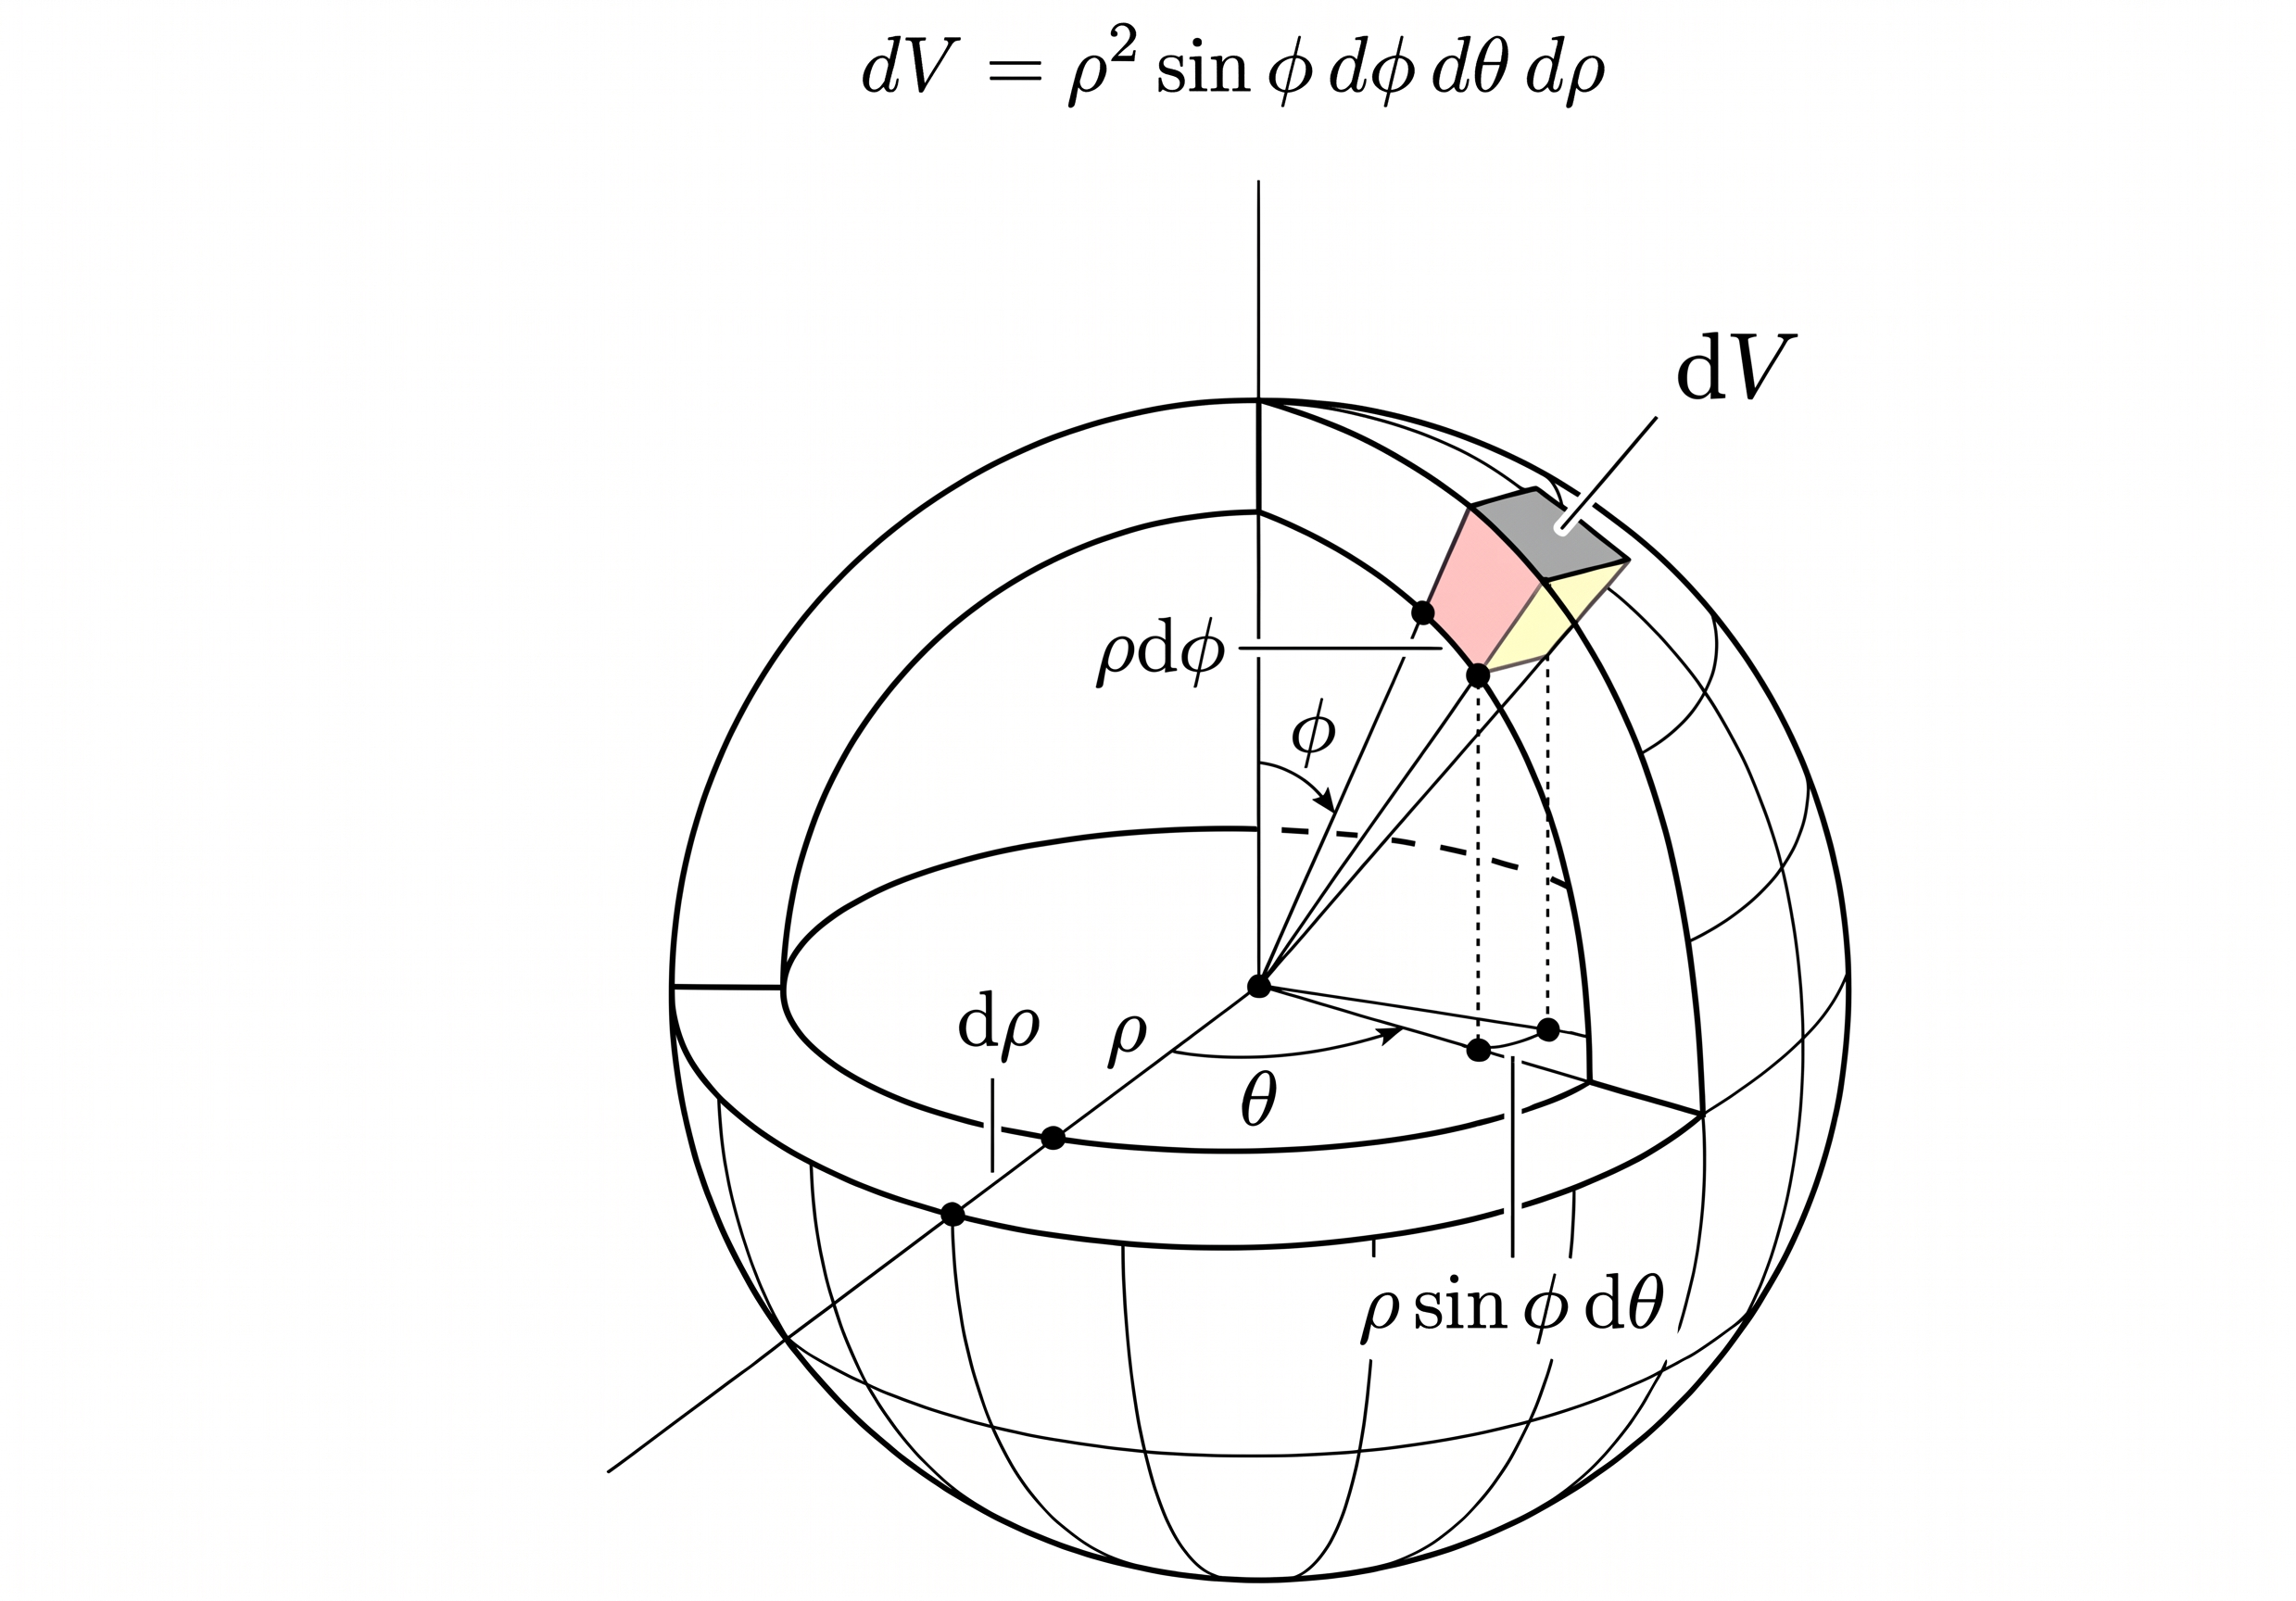
\includegraphics[width=0.8\textwidth]{figures/Spherical_Volume.png}
\caption{The spherical volume element is bounded by small changes in \(\rho\), \(\theta\), and \(\phi\).}
\label{fig:spherical_volume_element}
\end{figure}

Now find the small volume element.

A small spherical coordinate box has three side lengths, approximately:

\[
    d\rho
\]
in the radial direction,

\[
    \rho\,d\phi
\]
in the direction that changes \(\phi\), and

\[
    \rho\sin\phi\,d\theta
\]
in the direction that goes around the \(z\)-axis.



Multiplying these gives
\[
    dV
    =
    d\rho\cdot \rho\,d\phi\cdot \rho\sin\phi\,d\theta.
\]
So
\[
\boxed{
    dV=\rho^2\sin\phi\,d\rho\,d\phi\,d\theta.
}
\]


The factor \(\rho^2\) says that shells farther from the origin are larger.  The factor
\(\sin\phi\) says that angular pieces shrink near the poles.  Near \(\phi=0\), all values
of \(\theta\) crowd around the positive \(z\)-axis.

In form language, the same scale factor is
\[
\boxed{
    dx\wedge dy\wedge dz
    =
    \rho^2\sin\phi\,
    d\rho\wedge d\phi\wedge d\theta.
}
\]
For positive volume, we write
\[
    dV=\rho^2\sin\phi\,d\rho\,d\phi\,d\theta.
\]

\begin{example}[Volume of a ball]
Let \(B\) be the ball of radius \(4\) centered at the origin:
\[
    x^2+y^2+z^2\le16.
\]
In spherical coordinates, this is simply
\[
    0\le\rho\le4,\qquad
    0\le\phi\le\pi,\qquad
    0\le\theta\le2\pi.
\]
Therefore
\[
\begin{aligned}
\operatorname{Volume}(B)
&=
\int_0^{2\pi}\int_0^\pi\int_0^4
\rho^2\sin\phi\,d\rho\,d\phi\,d\theta\\
&=
\left(\int_0^{2\pi}d\theta\right)
\left(\int_0^\pi\sin\phi\,d\phi\right)
\left(\int_0^4\rho^2\,d\rho\right)\\
&=
(2\pi)(2)\left(\frac{64}{3}\right)\\
&=
\frac{256\pi}{3}.
\end{aligned}
\]
This matches
\[
    \frac43\pi(4)^3=\frac{256\pi}{3}.
\]
\end{example}

Again, the scale factor is not optional.  If we computed the unit ball without
\(\sin\phi\), we would get
\[
    \int_0^{2\pi}\int_0^\pi\int_0^1 \rho^2\,d\rho\,d\phi\,d\theta
    =
    \frac{2\pi^2}{3},
\]
not
\[
    \frac{4\pi}{3}.
\]
The missing \(\sin\phi\) would give too much weight to tiny angular pieces near the
poles.

\subsection{Balls, shells, and cones}

Spherical coordinates turn spheres into constant-\(\rho\) surfaces:
\[
    x^2+y^2+z^2=a^2
    \qquad\Longleftrightarrow\qquad
    \rho=a.
\]
So balls and shells become very simple.

\begin{example}[A spherical shell]
The shell between radius \(2\) and radius \(5\) is
\[
    2\le\rho\le5.
\]
With full angular range,
\[
    0\le\phi\le\pi,\qquad 0\le\theta\le2\pi.
\]
Its volume is
\[
\begin{aligned}
V
&=
\int_0^{2\pi}\int_0^\pi\int_2^5
\rho^2\sin\phi\,d\rho\,d\phi\,d\theta\\
&=
(2\pi)(2)\left[\frac{\rho^3}{3}\right]_2^5\\
&=
4\pi\cdot\frac{125-8}{3}\\
&=
156\pi.
\end{aligned}
\]
\end{example}

Cones also become simple, because a cone with vertex at the origin is a constant-angle
surface.  For example,
\[
    z=\sqrt{x^2+y^2}
\]
becomes
\[
    \rho\cos\phi=\rho\sin\phi.
\]
Away from the origin, this gives
\[
    \cos\phi=\sin\phi,
\]
so
\[
    \phi=\frac{\pi}{4}.
\]
The inside of the upper cone is
\[
    0\le\phi\le\frac{\pi}{4}.
\]

\begin{example}[A ball cut by a cone]
Find the volume inside the sphere
\[
    \rho\le3
\]
and inside the upper cone
\[
    z\ge \sqrt{x^2+y^2}.
\]
The cone is
\[
    0\le\phi\le\frac{\pi}{4}.
\]
The full rotation around the \(z\)-axis gives
\[
    0\le\theta\le2\pi.
\]
So
\[
\begin{aligned}
V
&=
\int_0^{2\pi}\int_0^{\pi/4}\int_0^3
\rho^2\sin\phi\,d\rho\,d\phi\,d\theta\\
&=
(2\pi)
\left(1-\cos\frac{\pi}{4}\right)
\left(9\right)\\
&=
18\pi\left(1-\frac{\sqrt2}{2}\right).
\end{aligned}
\]
Thus
\[
\boxed{
    V=18\pi\left(1-\frac{\sqrt2}{2}\right).
}
\]
\end{example}

A sphere fixes \(\rho\).  A cone fixes \(\phi\).  A vertical half-plane fixes \(\theta\).
That is the basic geometry of spherical bounds.

\subsection{Choosing the angular bounds}

The angle \(\theta\) is the same azimuth angle used in cylindrical coordinates.  It
describes the shadow in the \(xy\)-plane.

The angle \(\phi\) describes how far down from the positive \(z\)-axis the point lies.
It controls vertical opening.

\[
\begin{array}{c|c}
\text{condition} & \text{spherical meaning} \\ \hline
z\ge0 & 0\le\phi\le\pi/2\\[1mm]
z\le0 & \pi/2\le\phi\le\pi\\[1mm]
x\ge0,\ y\ge0 & 0\le\theta\le\pi/2\\[1mm]
\rho\le a & \text{inside sphere of radius }a\\[1mm]
z=\sqrt{x^2+y^2} & \phi=\pi/4
\end{array}
\]

\begin{example}[The first octant of a ball]
The first octant means
\[
    x\ge0,\qquad y\ge0,\qquad z\ge0.
\]
For the ball
\[
    \rho\le4,
\]
the bounds are
\[
    0\le\rho\le4,
    \qquad
    0\le\phi\le\frac{\pi}{2},
    \qquad
    0\le\theta\le\frac{\pi}{2}.
\]
The volume is
\[
\begin{aligned}
V
&=
\int_0^{\pi/2}\int_0^{\pi/2}\int_0^4
\rho^2\sin\phi\,d\rho\,d\phi\,d\theta\\
&=
\left(\frac{\pi}{2}\right)(1)\left(\frac{64}{3}\right)\\
&=
\frac{32\pi}{3}.
\end{aligned}
\]
This is one eighth of the full ball volume
\[
    \frac{256\pi}{3}.
\]
\end{example}

Spherical coordinates can also describe caps, where the radial lower bound is not zero.

\begin{example}[A spherical cap]
Find the volume inside the sphere
\[
    \rho\le3
\]
and above the plane
\[
    z=1.
\]
The plane becomes
\[
    \rho\cos\phi=1.
\]
Along a ray with angle \(\phi\), the plane is reached at
\[
    \rho=\sec\phi.
\]
For the ray to reach the sphere after crossing the plane, we need
\[
    \sec\phi\le3,
\]
or
\[
    \cos\phi\ge\frac13.
\]
Thus
\[
    0\le\phi\le\arccos\frac13.
\]
The bounds are
\[
    0\le\theta\le2\pi,
    \qquad
    0\le\phi\le\arccos\frac13,
    \qquad
    \sec\phi\le\rho\le3.
\]
So
\[
\boxed{
V=
\int_0^{2\pi}
\int_0^{\arccos(1/3)}
\int_{\sec\phi}^{3}
\rho^2\sin\phi\,d\rho\,d\phi\,d\theta.
}
\]
Compute:
\[
\begin{aligned}
V
&=
2\pi\int_0^{\arccos(1/3)}
\left[\frac{\rho^3}{3}\right]_{\sec\phi}^3
\sin\phi\,d\phi\\
&=
2\pi\int_0^{\arccos(1/3)}
\left(9-\frac13\sec^3\phi\right)\sin\phi\,d\phi.
\end{aligned}
\]
Let
\[
    \alpha=\arccos\frac13.
\]
Then
\[
    \cos\alpha=\frac13,
    \qquad
    \tan^2\alpha=8.
\]
Also,
\[
    \int_0^\alpha 9\sin\phi\,d\phi
    =
    9(1-\cos\alpha)=6,
\]
and
\[
    \frac13\int_0^\alpha \sec^3\phi\sin\phi\,d\phi
    =
    \frac13\int_0^\alpha \tan\phi\,\sec^2\phi\,d\phi
    =
    \frac16\tan^2\alpha
    =
    \frac43.
\]
Therefore
\[
    V=2\pi\left(6-\frac43\right)=\frac{28\pi}{3}.
\]
\end{example}

The angular bounds come from looking along rays from the origin.  A ray either enters
the solid immediately, enters after crossing a surface, or misses the solid.  Spherical
coordinates make us answer that ray question.

\subsection{Applications to gravitational and radial densities}

Many three-dimensional densities depend only on distance from a central point.  A
planet model, a gas cloud, and a radially symmetric charge distribution all have this
shape:
\[
    \delta=\delta(\rho).
\]
For a ball of radius \(a\), the total mass is
\[
\begin{aligned}
M
&=
\int_0^{2\pi}\int_0^\pi\int_0^a
\delta(\rho)\rho^2\sin\phi\,d\rho\,d\phi\,d\theta\\
&=
4\pi\int_0^a \delta(\rho)\rho^2\,d\rho.
\end{aligned}
\]
So
\[
\boxed{
    M=4\pi\int_0^a \delta(\rho)\rho^2\,d\rho.
}
\]
The angular part contributes \(4\pi\), and the radial part carries the real information.

\begin{example}[A simple model planet]
Suppose a planet has radius \(3\), and its density decreases linearly with distance from
the center:
\[
    \delta(\rho)=6-\rho,
    \qquad 0\le\rho\le3.
\]
Then
\[
\begin{aligned}
M
&=
4\pi\int_0^3(6-\rho)\rho^2\,d\rho\\
&=
4\pi\int_0^3(6\rho^2-\rho^3)\,d\rho\\
&=
4\pi\left[2\rho^3-\frac{\rho^4}{4}\right]_0^3\\
&=
4\pi\left(54-\frac{81}{4}\right)\\
&=
135\pi.
\end{aligned}
\]
Thus
\[
\boxed{
    M=135\pi.
}
\]
\end{example}

The same scale factor explains a familiar feature of inverse-square laws.  Suppose an
energy density in a spherical shell is
\[
    u(\rho)=\frac{10}{\rho^2},
    \qquad 1\le\rho\le4.
\]
The total energy in the shell is
\[
\begin{aligned}
E
&=
\int_0^{2\pi}\int_0^\pi\int_1^4
\frac{10}{\rho^2}\rho^2\sin\phi\,d\rho\,d\phi\,d\theta\\
&=
10(2\pi)(2)\int_1^4 d\rho\\
&=
120\pi.
\end{aligned}
\]
The \(\rho^2\) in the volume element cancels the \(1/\rho^2\) in the density.  Each
unit of radial thickness contributes the same amount.  Later, when we study flux, the
same geometric growth of spherical area will help explain why gravitational and electric
fields often have inverse-square form.

Cylindrical and spherical coordinates changed the shape of \(dV\), but not the meaning
of the integral.  A triple integral still adds tiny contributions through a solid.  Once we
can add density, the next questions are natural: Where is the mass balanced?  How far
is it spread from an axis?  How much charge or energy does the solid contain?  Those
are the applications that turn triple integrals from volume machines into physical
measuring tools.
\section{Applications of triple integrals}
\label{sec:11.5}

Sections \ref{sec:11.1}--\ref{sec:11.4} taught us how to add over a solid.  The
geometry changed from boxes to wedges, cylinders, cones, balls, and shells, but the
basic contribution always had the same shape:
\[
    \text{value near a point}\times \text{tiny volume}.
\]
Now the value near the point becomes physical.  It may be mass density, charge
density, energy density, or probability density.

Because spherical coordinates already use the letter \(\rho\), this section writes mass
density as
\[
    \delta(x,y,z).
\]

\subsection{Mass and density in space}

Imagine a clear gel block in a laboratory.  A chemical additive has settled unevenly, so
the density is larger near the top.  The block occupies
\[
    E=[0,4]\times[0,3]\times[0,2],
\]
and its density is
\[
    \delta(x,y,z)=2+z
\]
grams per cubic centimeter.

A small box near \((x,y,z)\) has mass approximately
\[
    \delta(x,y,z)\,\Delta V.
\]
Adding all those small masses gives
\[
    M=\iiint_E \delta(x,y,z)\,dV.
\]
For this block,
\[
\begin{aligned}
M
&=
\int_0^4\int_0^3\int_0^2 (2+z)\,dz\,dy\,dx\\
&=
\int_0^4\int_0^3
\left[2z+\frac{z^2}{2}\right]_0^2
\,dy\,dx\\
&=
\int_0^4\int_0^3 6\,dy\,dx\\
&=
72.
\end{aligned}
\]
So the total mass is
\[
\boxed{
    M=72.
}
\]

\begin{definition}[Mass from a density]
If a solid \(E\) has mass density
\[
    \delta(x,y,z),
\]
then its mass is
\[
\boxed{
    M=\iiint_E \delta(x,y,z)\,dV.
}
\]
\end{definition}

In oriented form notation, the same integral can be written
\[
    \iiint_E \delta(x,y,z)\,dx\wedge dy\wedge dz,
\]
when the solid is given the standard orientation.  For mass, however, we usually write
\(dV\), because mass uses positive volume.

\begin{example}[Mass of a cone with density depending on height]
A solid cone has height \(4\), radius \(4\), and density
\[
    \delta(x,y,z)=1+z.
\]
The cone has equation
\[
    0\le z\le 4-r
\]
in cylindrical coordinates.  Thus
\[
    0\le \theta\le 2\pi,
    \qquad
    0\le r\le4,
    \qquad
    0\le z\le4-r.
\]
The mass is
\[
\begin{aligned}
M
&=
\int_0^{2\pi}\int_0^4\int_0^{4-r}
(1+z)r\,dz\,dr\,d\theta\\
&=
2\pi\int_0^4
\left[z+\frac{z^2}{2}\right]_0^{4-r}
r\,dr\\
&=
2\pi\int_0^4
\left((4-r)+\frac12(4-r)^2\right)r\,dr.
\end{aligned}
\]
Expand:
\[
    (4-r)+\frac12(4-r)^2
    =
    4-r+8-4r+\frac12r^2
    =
    12-5r+\frac12r^2.
\]
So
\[
\begin{aligned}
M
&=
2\pi\int_0^4
\left(12r-5r^2+\frac12r^3\right)\,dr\\
&=
2\pi
\left[
6r^2-\frac53r^3+\frac18r^4
\right]_0^4\\
&=
2\pi
\left(
96-\frac{320}{3}+32
\right)\\
&=
2\pi\cdot\frac{64}{3}\\
&=
\frac{128\pi}{3}.
\end{aligned}
\]
Thus
\[
\boxed{
    M=\frac{128\pi}{3}.
}
\]
\end{example}

The density decides how much each small volume piece counts.  The geometry decides
where the pieces are.

\subsection{Center of mass}

Mass tells us how much matter there is.  The center of mass tells us where that matter
balances.

Return to the gel block
\[
    E=[0,4]\times[0,3]\times[0,2],
\]
with density
\[
    \delta(x,y,z)=2+z.
\]
The density depends only on height.  So symmetry already tells us
\[
    \bar x=2,
    \qquad
    \bar y=\frac32.
\]
But the \(z\)-coordinate of the center should be above the geometric middle \(z=1\),
because the block is denser near the top.

To find it, we compute the first moments:
\[
    N_x=\iiint_E x\delta\,dV,
    \qquad
    N_y=\iiint_E y\delta\,dV,
    \qquad
    N_z=\iiint_E z\delta\,dV.
\]
For this block,
\[
\begin{aligned}
N_x
&=
\int_0^4\int_0^3\int_0^2 x(2+z)\,dz\,dy\,dx\\
&=
\left(\int_0^4 x\,dx\right)
\left(\int_0^3 dy\right)
\left(\int_0^2(2+z)\,dz\right)\\
&=
8\cdot3\cdot6\\
&=
144.
\end{aligned}
\]
Similarly,
\[
\begin{aligned}
N_y
&=
\left(\int_0^4 dx\right)
\left(\int_0^3 y\,dy\right)
\left(\int_0^2(2+z)\,dz\right)\\
&=
4\cdot\frac92\cdot6\\
&=
108.
\end{aligned}
\]
For the height moment,
\[
\begin{aligned}
N_z
&=
\int_0^4\int_0^3\int_0^2 z(2+z)\,dz\,dy\,dx\\
&=
12\int_0^2(2z+z^2)\,dz\\
&=
12\left[z^2+\frac{z^3}{3}\right]_0^2\\
&=
12\left(4+\frac83\right)\\
&=
80.
\end{aligned}
\]
Since \(M=72\), the center of mass is
\[
\boxed{
    (\bar x,\bar y,\bar z)
    =
    \left(
    \frac{N_x}{M},\frac{N_y}{M},\frac{N_z}{M}
    \right)
    =
    \left(2,\frac32,\frac{10}{9}\right).
}
\]
As expected,
\[
    \bar z=\frac{10}{9}>1.
\]

\begin{figure}[h]
\centering
\begin{tikzpicture}[scale=0.8, >=stealth]
    \coordinate (O) at (0,0);
    \coordinate (A) at (4,0);
    \coordinate (B) at (5.2,1.1);
    \coordinate (C) at (1.2,1.1);
    \coordinate (D) at (0,2.6);
    \coordinate (E) at (4,2.6);
    \coordinate (F) at (5.2,3.7);
    \coordinate (G) at (1.2,3.7);

    \draw[fill=gray!8, thick] (O)--(A)--(B)--(C)--cycle;
    \draw[fill=gray!15, thick] (D)--(E)--(F)--(G)--cycle;
    \draw[thick] (O)--(D);
    \draw[thick] (A)--(E);
    \draw[thick] (B)--(F);
    \draw[thick] (C)--(G);

    \foreach \z/\shade in {0.45/10,0.9/16,1.35/23,1.8/30,2.25/38} {
        \draw[fill=blue!\shade, draw=none, opacity=0.45]
            (0,\z) -- (4,\z) -- (5.2,{1.1+\z}) -- (1.2,{1.1+\z}) -- cycle;
    }

    \fill[red!70!black] (2.67,1.92) circle (3pt);
    \node[right] at (2.75,1.92) {center of mass};

    \node at (2,-0.55) {\(x\)-direction};
    \node[left] at (0,1.3) {\(z\)};
    \node at (2.6,-1.05) {denser layers near the top raise \(\bar z\)};
\end{tikzpicture}
\caption{When density increases with height, the center of mass moves upward.}
\end{figure}

\begin{definition}[Center of mass in space]
Let \(E\) be a solid with density \(\delta(x,y,z)\), and suppose
\[
    M=\iiint_E \delta\,dV>0.
\]
Define the first moments
\[
    N_x=\iiint_E x\delta\,dV,
    \qquad
    N_y=\iiint_E y\delta\,dV,
    \qquad
    N_z=\iiint_E z\delta\,dV.
\]
Then the center of mass is
\[
\boxed{
    (\bar x,\bar y,\bar z)
    =
    \left(
        \frac{N_x}{M},
        \frac{N_y}{M},
        \frac{N_z}{M}
    \right).
}
\]
\end{definition}

The condition \(M>0\) matters.  A real mass density is nonnegative, and if there is any
material at all, then \(M>0\).  But for signed quantities, such as electric charge, the
same formula can break.

\begin{example}[Why positive total mass is needed]
Suppose a cube contains equal amounts of positive and negative charge.  A signed
charge density \(q\) might satisfy
\[
    \iiint_E q\,dV=0.
\]
The expression
\[
    \frac{\iiint_E xq\,dV}{\iiint_E q\,dV}
\]
then tries to divide by zero.  There may be a meaningful center of positive charge and a
meaningful center of negative charge, but there is no center of ``total signed charge''
given by this quotient.

So the center of mass formula belongs to a positive finite mass distribution.
\end{example}

\subsection{Moment of inertia}

Center of mass measures balance.  Moment of inertia measures resistance to rotation.

A point mass far from an axis is harder to spin than the same point mass near the axis.
The distance is squared, so far-away material counts strongly.

If a small volume piece has mass
\[
    \delta\,dV
\]
and its distance from the axis is \(s\), then its small contribution to moment of inertia
is
\[
    s^2\delta\,dV.
\]

\begin{definition}[Moment of inertia about an axis]
For a solid \(E\) with density \(\delta(x,y,z)\), the moment of inertia about an axis
is
\[
\boxed{
    I=\iiint_E s^2\delta(x,y,z)\,dV,
}
\]
where \(s\) is the distance from \((x,y,z)\) to the axis.
\end{definition}

For the coordinate axes,
\[
\boxed{
    I_x=\iiint_E (y^2+z^2)\delta\,dV,
}
\]
\[
\boxed{
    I_y=\iiint_E (x^2+z^2)\delta\,dV,
}
\]
and
\[
\boxed{
    I_z=\iiint_E (x^2+y^2)\delta\,dV.
}
\]

\begin{example}[A solid cylinder spinning around its axis]
A solid cylinder has radius \(2\), height \(3\), and constant density \(5\).  It spins
around its central \(z\)-axis.

In cylindrical coordinates,
\[
    0\le r\le2,
    \qquad
    0\le\theta\le2\pi,
    \qquad
    0\le z\le3.
\]
The distance to the \(z\)-axis is
\[
    s=r.
\]
So
\[
\begin{aligned}
I_z
&=
\int_0^{2\pi}\int_0^2\int_0^3
r^2\cdot 5\cdot r\,dz\,dr\,d\theta\\
&=
5\int_0^{2\pi}\int_0^2\int_0^3
r^3\,dz\,dr\,d\theta\\
&=
5(2\pi)(3)\int_0^2 r^3\,dr\\
&=
30\pi\left[\frac{r^4}{4}\right]_0^2\\
&=
30\pi\cdot4\\
&=
120\pi.
\end{aligned}
\]
Thus
\[
\boxed{
    I_z=120\pi.
}
\]

The mass of the cylinder is
\[
    M=5\pi(2)^2(3)=60\pi.
\]
So
\[
    I_z=\frac12M(2)^2,
\]
which matches the familiar physics formula for a solid cylinder.
\end{example}

\begin{figure}[h]
\centering
\begin{tikzpicture}[scale=0.9, >=stealth]
    % Define the symmetric horizontal shading (distance from vertical axis is |x|)
    \pgfdeclarehorizontalshading{densityshading}{100bp}{
        color(0bp)=(red!80!black);     % At x = -R, color corresponds to (-R)^2
        color(25bp)=(red!40!white);    % Intermediate point for non-linear transition
        color(50bp)=(white);          % At x = 0 (axis), color is minimal
        color(75bp)=(red!40!white);    % Non-linear intermediate
        color(100bp)=(red!80!black)    % At x = +R, color is max
    }

    % Fill the circle with the custom shading
    \begin{scope}
        \clip (0,0) circle (2.5);
        \shade[shading=densityshading, shading angle=0] (-2.5,-2.5) rectangle (2.5,2.5);
    \end{scope}

    % Boundary circle and guidelinles
    \draw[thick] (0,0) circle (2.5);
    \draw[gray!40, thin] (0,0) circle (0.8); % Gray slightly darkened for contrast
    \draw[gray!40, thin] (0,0) circle (1.6);

    % Axes and point with vector
    \draw[->] (-3.2,0) -- (3.4,0) node[right] {\(x\)};
    \draw[->] (0,-3.2) -- (0,3.4) node[above] {\(y\)};
    
    \draw[->, thick] (0,0) -- (35:1.7) node[midway, above] {\(r\)};
    \fill (35:1.7) circle (2pt);

    % Main axis line
    \draw[very thick, blue!60!black] (0,-3) -- (0,3);
    \node[blue!60!black, left] at (0,2.9) {axis};

    % Descriptive label
    \node at (0,-3.8) {material farther from the axis contributes \(r^2\) times as much};
\end{tikzpicture}
\caption{For rotation about the \(z\)-axis, the distance factor is \(r^2=x^2+y^2\).}
\end{figure}

Moment of inertia is an integral because a solid is made of many tiny masses, each at
its own distance from the axis.

\subsection{Total charge and total energy}

Mass density is nonnegative.  Charge density can be positive or negative.  Energy
density is usually nonnegative.

If \(q(x,y,z)\) is charge density, then total charge is
\[
\boxed{
    Q=\iiint_E q(x,y,z)\,dV.
}
\]
If \(u(x,y,z)\) is energy density, then total energy is
\[
\boxed{
    \mathcal E=\iiint_E u(x,y,z)\,dV.
}
\]

\begin{example}[Positive and negative charge can cancel]
A charged cylinder has radius \(1\), height \(2\), and charge density
\[
    q(x,y,z)=z-1.
\]
The lower half has negative charge, and the upper half has positive charge.

In cylindrical coordinates,
\[
    0\le r\le1,
    \qquad
    0\le\theta\le2\pi,
    \qquad
    0\le z\le2.
\]
The total charge is
\[
\begin{aligned}
Q
&=
\int_0^{2\pi}\int_0^1\int_0^2
(z-1)r\,dz\,dr\,d\theta\\
&=
\left(\int_0^{2\pi}d\theta\right)
\left(\int_0^1 r\,dr\right)
\left(\int_0^2(z-1)\,dz\right).
\end{aligned}
\]
But
\[
    \int_0^2(z-1)\,dz
    =
    \left[\frac{z^2}{2}-z\right]_0^2
    =
    2-2
    =
    0.
\]
Therefore
\[
\boxed{
    Q=0.
}
\]
The cylinder is not uncharged everywhere.  Its total signed charge is zero because the
positive and negative parts cancel.
\end{example}

\begin{example}[Energy stored in a spherical battery material]
A ball of radius \(2\) has energy density depending only on distance from the center:
\[
    u(\rho)=10\left(1-\frac{\rho}{2}\right),
    \qquad
    0\le \rho\le2.
\]
The density is largest at the center and drops to \(0\) at the surface.

Using spherical coordinates,
\[
\begin{aligned}
\mathcal E
&=
\int_0^{2\pi}\int_0^\pi\int_0^2
10\left(1-\frac{\rho}{2}\right)\rho^2\sin\phi
\,d\rho\,d\phi\,d\theta\\
&=
4\pi\cdot10\int_0^2
\left(\rho^2-\frac12\rho^3\right)\,d\rho\\
&=
40\pi
\left[
\frac{\rho^3}{3}-\frac{\rho^4}{8}
\right]_0^2\\
&=
40\pi\left(\frac83-2\right)\\
&=
\frac{80\pi}{3}.
\end{aligned}
\]
So
\[
\boxed{
    \mathcal E=\frac{80\pi}{3}.
}
\]
\end{example}

The same triple integral notation covers mass, charge, and energy.  The units of the
integrand tell us what is being added.

\[
\begin{array}{c|c|c}
\text{Density} & \text{Units} & \text{Integral} \\ \hline
\delta(x,y,z) & \text{mass}/\text{volume} &
\displaystyle M=\iiint_E \delta\,dV \\[3mm]
q(x,y,z) & \text{charge}/\text{volume} &
\displaystyle Q=\iiint_E q\,dV \\[3mm]
u(x,y,z) & \text{energy}/\text{volume} &
\displaystyle \mathcal E=\iiint_E u\,dV
\end{array}
\]

\subsection{Probability in three dimensions}

A probability density is another kind of density.  Instead of mass per volume or charge
per volume, it gives probability per volume.

If a random point is chosen in a solid region \(E\), a probability density \(p(x,y,z)\)
must satisfy two conditions:
\[
    p(x,y,z)\ge0
\]
and
\[
    \iiint_E p(x,y,z)\,dV=1.
\]
Then the probability that the point lies in a smaller region \(A\subseteq E\) is
\[
\boxed{
    \operatorname{Prob}(A)=\iiint_A p(x,y,z)\,dV.
}
\]

\begin{example}[A random point more likely near the top of a box]
A random point is chosen in the unit cube
\[
    0\le x\le1,
    \qquad
    0\le y\le1,
    \qquad
    0\le z\le1.
\]
Suppose the density has the form
\[
    p(x,y,z)=C(1+z).
\]
First find \(C\).  We need
\[
    \iiint_E C(1+z)\,dV=1.
\]
Thus
\[
\begin{aligned}
1
&=
C\int_0^1\int_0^1\int_0^1(1+z)\,dz\,dy\,dx\\
&=
C\left[z+\frac{z^2}{2}\right]_0^1\\
&=
C\cdot\frac32.
\end{aligned}
\]
So
\[
\boxed{
    C=\frac23.
}
\]

Now find the probability that
\[
    z\le\frac12.
\]
This is
\[
\begin{aligned}
\operatorname{Prob}\left(z\le\frac12\right)
&=
\int_0^1\int_0^1\int_0^{1/2}
\frac23(1+z)\,dz\,dy\,dx\\
&=
\frac23
\left[z+\frac{z^2}{2}\right]_0^{1/2}\\
&=
\frac23\left(\frac12+\frac18\right)\\
&=
\frac{5}{12}.
\end{aligned}
\]
So
\[
\boxed{
    \operatorname{Prob}\left(z\le\frac12\right)=\frac{5}{12}.
}
\]
Even though the lower half of the cube has half the volume, it has less than half the
probability, because the density increases with \(z\).
\end{example}

The conditions
\[
    p\ge0,
    \qquad
    \iiint_E p\,dV=1
\]
are not cosmetic.  Without them, the word probability loses its meaning.

\begin{example}[Why probability densities must be nonnegative and normalized]
On the unit cube, the function
\[
    p(x,y,z)=2
\]
is nonnegative, but
\[
    \iiint_E 2\,dV=2.
\]
It assigns total probability \(2\), not \(1\), so it is not a probability density.

The function
\[
    q(x,y,z)=2z-1
\]
has total integral \(0\), and it is negative when \(z<1/2\).  It cannot describe
probability, because some regions would receive negative probability.

A probability density is an ordinary density with two extra promises: no negative
amounts, and total amount exactly \(1\).
\end{example}

This last example points beyond three dimensions.  A random point might have four
coordinates, or ten, or a hundred.  A gas molecule has position and velocity.  A data
point may have many measured features.  The adding idea does not stop at three
coordinates.  What changes is harder to draw: a tiny piece is no longer a rectangle or a
box we can picture.  It is still a product of tiny coordinate lengths.

\section{Higher-dimensional integrals}
\label{sec:11.6}

The probability example at the end of Section \ref{sec:11.5} did not really care that the
random point had three coordinates.  A system may have many coordinates:
\[
    x_1,x_2,\ldots,x_n.
\]
A triple integral is the case \(n=3\).  Higher-dimensional integrals follow the same
adding rule, but the pictures become less trustworthy.

The wedge notation in this book will stay in dimensions \(1\), \(2\), and \(3\).  In this
optional section, we write
\[
    dV_n
\]
for positive \(n\)-dimensional volume.

\subsection{What changes in \texorpdfstring{\(\mathbb R^n\)}{Rn}}

A point in \(\mathbb R^n\) is written
\[
    \mathbf x=(x_1,x_2,\ldots,x_n).
\]
A rectangular box in \(\mathbb R^n\) has the form
\[
    B=[a_1,b_1]\times[a_2,b_2]\times\cdots\times[a_n,b_n].
\]
Its side lengths are
\[
    b_1-a_1,\quad b_2-a_2,\quad \ldots,\quad b_n-a_n.
\]
Its \(n\)-dimensional volume is
\[
\boxed{
    \operatorname{Vol}_n(B)
    =
    (b_1-a_1)(b_2-a_2)\cdots(b_n-a_n).
}
\]

A small coordinate box has side lengths
\[
    \Delta x_1,\Delta x_2,\ldots,\Delta x_n.
\]
Its small volume is
\[
    \Delta V_n
    =
    \Delta x_1\Delta x_2\cdots\Delta x_n.
\]
So the Riemann sum for a function
\[
    f(x_1,\ldots,x_n)
\]
has the form
\[
    \sum f(\mathbf x_i^*)\,\Delta V_{n,i}.
\]
If these sums settle to a single value, we write
\[
\boxed{
    \int_E f(\mathbf x)\,dV_n.
}
\]

\begin{example}[A four-dimensional quality-control box]
A machine produces parts with four measured deviations:
\[
    x_1,\quad x_2,\quad x_3,\quad x_4.
\]
Suppose each deviation is allowed to lie between \(-1\) and \(1\).  The acceptable
region is the four-dimensional box
\[
    B=[-1,1]^4.
\]
Its volume is
\[
    \operatorname{Vol}_4(B)=2\cdot2\cdot2\cdot2=16.
\]

If all points in \(B\) are equally likely, the probability density is constant:
\[
    p=\frac1{16}.
\]
The probability that every deviation lies between \(-1/2\) and \(1/2\) is
\[
\begin{aligned}
\operatorname{Prob}\left([-1/2,1/2]^4\right)
&=
\int_{[-1/2,1/2]^4}\frac1{16}\,dV_4\\
&=
\frac1{16}\cdot
(1\cdot1\cdot1\cdot1)\\
&=
\frac1{16}.
\end{aligned}
\]
Each coordinate range was cut in half, but the four-dimensional volume was cut by
\[
    \left(\frac12\right)^4.
\]
This is the first hint that high-dimensional size shrinks faster than our eyes expect.
\end{example}

\begin{definition}[Higher-dimensional integral]
Let \(E\subseteq\mathbb R^n\).  If Riemann sums
\[
    \sum f(\mathbf x_i^*)\,\Delta V_{n,i}
\]
approach one number as the small \(n\)-dimensional boxes shrink, independent of the
sample points, then that number is the integral of \(f\) over \(E\):
\[
\boxed{
    \int_E f(\mathbf x)\,dV_n.
}
\]
\end{definition}

For \(n=1\), this is an ordinary single-variable integral.  For \(n=2\), it is a double
integral.  For \(n=3\), it is a triple integral.

\subsection{Product regions and Fubini's theorem}

The easiest higher-dimensional regions are boxes and product regions, because each
coordinate has its own interval.

For example, let
\[
    B=[0,2]\times[0,3]\times[0,1]\times[0,4].
\]
Then
\[
    \operatorname{Vol}_4(B)=2\cdot3\cdot1\cdot4=24.
\]

Now compute
\[
    I=\int_B (x_1+x_4)\,dV_4.
\]
Using iterated integrals,
\[
\begin{aligned}
I
&=
\int_0^2\int_0^3\int_0^1\int_0^4
(x_1+x_4)\,dx_4\,dx_3\,dx_2\,dx_1.
\end{aligned}
\]
Split the integral into two pieces:
\[
    I
    =
    \int_B x_1\,dV_4+\int_B x_4\,dV_4.
\]
For the \(x_1\)-piece,
\[
\begin{aligned}
\int_B x_1\,dV_4
&=
\left(\int_0^2 x_1\,dx_1\right)
\left(\int_0^3 dx_2\right)
\left(\int_0^1 dx_3\right)
\left(\int_0^4 dx_4\right)\\
&=
2\cdot3\cdot1\cdot4\\
&=
24.
\end{aligned}
\]
For the \(x_4\)-piece,
\[
\begin{aligned}
\int_B x_4\,dV_4
&=
\left(\int_0^2 dx_1\right)
\left(\int_0^3 dx_2\right)
\left(\int_0^1 dx_3\right)
\left(\int_0^4 x_4\,dx_4\right)\\
&=
2\cdot3\cdot1\cdot8\\
&=
48.
\end{aligned}
\]
Thus
\[
\boxed{
    I=72.
}
\]
The average value of \(x_1+x_4\) over the box is
\[
    \frac{72}{24}=3.
\]
That is the average of \(x_1\), which is \(1\), plus the average of \(x_4\), which is
\(2\).

\begin{theorem}[Fubini's theorem for boxes in \(\mathbb R^n\)]
Let
\[
    B=[a_1,b_1]\times\cdots\times[a_n,b_n],
\]
and suppose \(f\) is continuous on \(B\).  Then
\[
\boxed{
    \int_B f(\mathbf x)\,dV_n
}
\]
can be computed as an iterated integral in any order.

For example,
\[
\boxed{
\int_B f\,dV_n
=
\int_{a_1}^{b_1}\cdots\int_{a_n}^{b_n}
f(x_1,\ldots,x_n)\,dx_n\cdots dx_1.
}
\]
\end{theorem}

Continuity is a safe condition.  It is stronger than necessary, but it keeps the adding
process well-behaved.

\begin{example}[A nonintegrable function still breaks the story]
On the unit box
\[
    [0,1]^n,
\]
define
\[
    q(x_1,\ldots,x_n)
    =
    \begin{cases}
    1, & x_1\text{ is rational},\\
    0, & x_1\text{ is irrational}.
    \end{cases}
\]
Every small \(n\)-dimensional box contains points with rational \(x_1\) and points with
irrational \(x_1\).  The upper sums are always \(1\), and the lower sums are always
\(0\).

So the Riemann integral does not exist.  Fubini's theorem cannot rescue an integral
that was never there.
\end{example}

There is a useful special case when the function factors.  If
\[
    f(x_1,\ldots,x_n)=g_1(x_1)g_2(x_2)\cdots g_n(x_n),
\]
then on a box,
\[
\boxed{
    \int_B f\,dV_n
    =
    \left(\int_{a_1}^{b_1}g_1(x_1)\,dx_1\right)
    \cdots
    \left(\int_{a_n}^{b_n}g_n(x_n)\,dx_n\right).
}
\]
The integral separates because the variables separate.

\begin{example}[A separated density]
Let
\[
    f(x_1,x_2,x_3,x_4)=e^{-x_1}(1+x_2)x_3^2
\]
on
\[
    [0,1]\times[0,2]\times[0,3]\times[0,4].
\]
The function does not depend on \(x_4\), so the \(x_4\)-integral contributes a factor
of \(4\).  We get
\[
\begin{aligned}
\int f\,dV_4
&=
\left(\int_0^1e^{-x_1}\,dx_1\right)
\left(\int_0^2(1+x_2)\,dx_2\right)
\left(\int_0^3x_3^2\,dx_3\right)
\left(\int_0^4 dx_4\right)\\
&=
(1-e^{-1})(4)(9)(4)\\
&=
144(1-e^{-1}).
\end{aligned}
\]
\end{example}

The arithmetic looks familiar because Fubini turns one higher-dimensional adding
problem into several one-dimensional ones.

\subsection{Volumes of higher-dimensional balls and boxes}

Boxes are easy in every dimension:
\[
    \operatorname{Vol}_n([0,L]^n)=L^n.
\]
Balls are subtler.

The \(n\)-dimensional ball of radius \(R\) is
\[
    B_n(R)=
    \left\{
    (x_1,\ldots,x_n):
    x_1^2+\cdots+x_n^2\le R^2
    \right\}.
\]
For the first few dimensions:
\[
\begin{array}{c|c|c}
n & B_n(R) & \operatorname{Vol}_n(B_n(R)) \\ \hline
1 & \text{interval} & 2R\\[1mm]
2 & \text{disk} & \pi R^2\\[1mm]
3 & \text{solid ball} & \dfrac43\pi R^3
\end{array}
\]

The four-dimensional ball cannot be drawn, but it can be sliced.

Let
\[
    B_4(1)=
    \{(x,y,z,w):x^2+y^2+z^2+w^2\le1\}.
\]
Fix \(w\).  Then the remaining variables satisfy
\[
    x^2+y^2+z^2\le1-w^2.
\]
That is a three-dimensional ball of radius
\[
    \sqrt{1-w^2}.
\]
Its volume is
\[
    \frac43\pi(1-w^2)^{3/2}.
\]
So
\[
\begin{aligned}
\operatorname{Vol}_4(B_4(1))
&=
\int_{-1}^{1}
\frac43\pi(1-w^2)^{3/2}\,dw.
\end{aligned}
\]
Use
\[
    w=\sin u.
\]
Then
\[
    dw=\cos u\,du,
    \qquad
    (1-w^2)^{3/2}=\cos^3u,
\]
and \(u\) runs from \(-\pi/2\) to \(\pi/2\).  Therefore
\[
\begin{aligned}
\operatorname{Vol}_4(B_4(1))
&=
\frac43\pi
\int_{-\pi/2}^{\pi/2}\cos^4u\,du.
\end{aligned}
\]
Since
\[
    \cos^4u=\frac{3+4\cos(2u)+\cos(4u)}{8},
\]
we have
\[
    \int_{-\pi/2}^{\pi/2}\cos^4u\,du=\frac{3\pi}{8}.
\]
Thus
\[
\boxed{
    \operatorname{Vol}_4(B_4(1))
    =
    \frac43\pi\cdot\frac{3\pi}{8}
    =
    \frac{\pi^2}{2}.
}
\]

Scaling by \(R\) in all four coordinates multiplies four-dimensional volume by
\(R^4\).  So
\[
\boxed{
    \operatorname{Vol}_4(B_4(R))
    =
    \frac{\pi^2}{2}R^4.
}
\]

The pattern continues:
\[
\begin{array}{c|c}
n & \operatorname{Vol}_n(B_n(R)) \\ \hline
1 & 2R\\[1mm]
2 & \pi R^2\\[1mm]
3 & \dfrac43\pi R^3\\[2mm]
4 & \dfrac{\pi^2}{2}R^4\\[2mm]
5 & \dfrac{8\pi^2}{15}R^5
\end{array}
\]

The formula has a compact version involving the gamma function, but the main idea is
already visible: higher-dimensional balls can be studied by slicing them into
lower-dimensional balls.

\subsection{Why high-dimensional geometry feels surprising}

High-dimensional geometry often disagrees with three-dimensional intuition.  The
reason is not mysterious.  Powers grow and shrink quickly.

For an \(n\)-dimensional ball, scaling the radius by \(a\) scales volume by
\[
    a^n.
\]
So the ball of half the radius has volume fraction
\[
\boxed{
    \left(\frac12\right)^n.
}
\]
In three dimensions, that fraction is
\[
    \frac18.
\]
In ten dimensions, it is
\[
    \frac1{1024}.
\]
In one hundred dimensions, it is
\[
    2^{-100}.
\]
So in high dimensions, very little of a ball's volume lies near the center.  Most of it
sits close to the outer shell.

The cube gives another surprise.  The cube
\[
    [-1,1]^n
\]
has volume
\[
    2^n.
\]
Its corners have distance
\[
    \sqrt{1^2+1^2+\cdots+1^2}=\sqrt n
\]
from the origin.  As \(n\) grows, the corners move farther and farther away, even
though every coordinate still lies between \(-1\) and \(1\).

In four dimensions, the ball of radius \(1\) inside the cube \([-1,1]^4\) has volume
\[
    \frac{\pi^2}{2}.
\]
The cube has volume
\[
    16.
\]
So the fraction occupied by the ball is
\[
    \frac{\pi^2/2}{16}
    =
    \frac{\pi^2}{32}
    \approx 0.31.
\]
Already by dimension \(4\), much of the cube lies outside the inscribed ball, toward
the corners.

These facts matter in probability, statistics, data science, and physics.  A point with
many coordinates does not behave like a point in a drawing.  Volume migrates toward
boundaries, corners, and shells.

But the integral itself has not changed.  It still adds tiny contributions.  The hard
part is describing how a small coordinate box in one system becomes a small piece in
another system.  We have already met two answers:
\[
    dV=r\,dr\,d\theta\,dz
\]
and
\[
    dV=\rho^2\sin\phi\,d\rho\,d\phi\,d\theta.
\]
Those factors were not tricks for cylinders and spheres.  They are examples of a
single rule.  Chapter \ref{ch:12} finds that rule by looking at how a coordinate map
stretches tiny boxes, and the determinant returns as the scale factor.
\section{Chapter review and applications}
\label{sec:11.7}

Chapter \ref{ch:11} took the adding idea one dimension higher.  A double integral
adds over a region in the plane:
\[
    f(x,y)\,dA.
\]
A triple integral adds over a solid:
\[
    f(x,y,z)\,dV.
\]
The tiny pieces changed from rectangles to boxes.  The story did not change:
\[
    \text{value near a point}\times \text{tiny volume}.
\]

The hard part is rarely the antiderivative.  The hard part is describing the solid without
counting too much or too little.

\subsection{Skills: triple integrals in several coordinate systems}

A triple integral begins with one question:
\[
    \text{What solid am I adding over?}
\]
After that, the coordinate system should serve the geometry.

\begin{figure}[h]
\centering
\begin{tikzpicture}[scale=0.88, >=stealth]
    \node[draw, rounded corners, align=center, minimum width=4.4cm, minimum height=0.9cm]
        (start) at (0,0) {Triple integral\\ \(\displaystyle \iiint_E f\,dV\)};

    % Widened from -5.2 to -5.9
    \node[draw, rounded corners, align=center, minimum width=4.4cm, minimum height=0.9cm]
        (rect) at (-5.9,-2) {Boxes, wedges, slabs\\ rectangular coordinates};

    \node[draw, rounded corners, align=center, minimum width=4.4cm, minimum height=0.9cm]
        (cyl) at (0,-2) {Cylinders, cones, tubes\\ cylindrical coordinates};

    % Widened from 5.2 to 5.9
    \node[draw, rounded corners, align=center, minimum width=4.4cm, minimum height=0.9cm]
        (sph) at (5.9,-2) {Balls, shells, central symmetry\\ spherical coordinates};

    \node[draw, rounded corners, align=center, minimum width=4.4cm, minimum height=0.9cm]
        (app) at (-2.8,-4.5) {Mass, charge, energy,\\ probability};

    \node[draw, rounded corners, align=center, minimum width=4.4cm, minimum height=0.9cm]
        (hd) at (2.8,-4.5) {Higher dimensions\\ product boxes and slicing};

    \draw[->, thick] (start) -- (rect);
    \draw[->, thick] (start) -- (cyl);
    \draw[->, thick] (start) -- (sph);

    \draw[->, thick] (rect) -- (app);
    \draw[->, thick] (cyl) -- (app);
    \draw[->, thick] (sph) -- (app);

    \draw[->, thick] (app) -- (hd);
\end{tikzpicture}
\caption{Choose coordinates by listening to the shape of the solid.}
\end{figure}
The main volume elements are:

\[
\begin{array}{c|c|c}
\text{Coordinates} & \text{Conversion} & \text{Volume element} \\ \hline
\text{rectangular} &
(x,y,z) &
dV=dx\,dy\,dz
\\[2mm]
\text{cylindrical} &
x=r\cos\theta,\quad y=r\sin\theta,\quad z=z &
dV=r\,dr\,d\theta\,dz
\\[2mm]
\text{spherical} &
x=\rho\sin\phi\cos\theta,\quad
y=\rho\sin\phi\sin\theta,\quad
z=\rho\cos\phi &
dV=\rho^2\sin\phi\,d\rho\,d\phi\,d\theta
\end{array}
\]

The oriented version of rectangular volume is
\[
    dx\wedge dy\wedge dz.
\]
For ordinary volume, mass, probability, and energy, we use positive volume:
\[
    dV.
\]
For orientation-sensitive integrals later in the book, the wedge notation will remember
the order of the directions.

Here are the main application formulas from the chapter.

\[
\begin{array}{c|c}
\text{Quantity} & \text{Triple integral} \\ \hline
\text{volume of }E
&
\displaystyle
\operatorname{Vol}(E)=\iiint_E 1\,dV
\\[3mm]
\text{mass from density }\delta
&
\displaystyle
M=\iiint_E \delta\,dV
\\[3mm]
\text{center of mass}
&
\displaystyle
(\bar x,\bar y,\bar z)
=
\left(
\frac{\iiint_E x\delta\,dV}{M},
\frac{\iiint_E y\delta\,dV}{M},
\frac{\iiint_E z\delta\,dV}{M}
\right)
\\[5mm]
\text{moment of inertia about the }z\text{-axis}
&
\displaystyle
I_z=\iiint_E (x^2+y^2)\delta\,dV
\\[4mm]
\text{total charge from charge density }q
&
\displaystyle
Q=\iiint_E q\,dV
\\[3mm]
\text{total energy from energy density }u
&
\displaystyle
\mathcal E=\iiint_E u\,dV
\\[3mm]
\text{probability of a region }A
&
\displaystyle
\operatorname{Prob}(A)=\iiint_A p\,dV
\end{array}
\]

A probability density must satisfy
\[
    p\ge0
\]
and
\[
    \iiint_E p\,dV=1.
\]

\subsection{Worked review example: a wedge with density}

A storage wedge has rectangular floor
\[
    0\le x\le2,\qquad 0\le y\le1,
\]
and slanted roof
\[
    z=4-x-y.
\]
The floor is
\[
    z=0.
\]
Its density is
\[
    \delta(x,y,z)=1+z.
\]
Find the mass.

The solid is
\[
    E=
    \{(x,y,z):0\le x\le2,\ 0\le y\le1,\ 0\le z\le4-x-y\}.
\]
So
\[
\begin{aligned}
M
&=
\int_0^2\int_0^1\int_0^{4-x-y}
(1+z)\,dz\,dy\,dx\\
&=
\int_0^2\int_0^1
\left[
z+\frac12z^2
\right]_0^{4-x-y}
\,dy\,dx\\
&=
\int_0^2\int_0^1
\left(
(4-x-y)+\frac12(4-x-y)^2
\right)dy\,dx.
\end{aligned}
\]
Expand the integrand:
\[
    (4-x-y)+\frac12(4-x-y)^2
    =
    12-5x-5y+\frac12x^2+xy+\frac12y^2.
\]
Now integrate in \(y\):
\[
\begin{aligned}
\int_0^1
\left(
12-5x-5y+\frac12x^2+xy+\frac12y^2
\right)dy
&=
\frac{29}{3}-\frac92x+\frac12x^2.
\end{aligned}
\]
Then
\[
\begin{aligned}
M
&=
\int_0^2
\left(
\frac{29}{3}-\frac92x+\frac12x^2
\right)dx\\
&=
\frac{58}{3}-9+\frac43\\
&=
\frac{35}{3}.
\end{aligned}
\]
Thus
\[
\boxed{
    M=\frac{35}{3}.
}
\]

The bounds came from the geometry.  The integrand came from the density.  The
calculation only came after both were clear.

\subsection{Worked review example: a round tank in cylindrical coordinates}

A round tank has radius \(2\).  Its floor is
\[
    z=0,
\]
and its roof height depends on distance from the central axis:
\[
    z=3+\frac r2.
\]
The density is
\[
    \delta(r,z)=1+r.
\]
Find the mass.

The solid is rotationally symmetric, so cylindrical coordinates fit:
\[
    0\le\theta\le2\pi,
    \qquad
    0\le r\le2,
    \qquad
    0\le z\le 3+\frac r2.
\]
Remember the volume factor:
\[
    dV=r\,dz\,dr\,d\theta.
\]
So
\[
\begin{aligned}
M
&=
\int_0^{2\pi}\int_0^2\int_0^{3+r/2}
(1+r)r\,dz\,dr\,d\theta\\
&=
2\pi\int_0^2
(1+r)r\left(3+\frac r2\right)dr.
\end{aligned}
\]
Expand:
\[
    (1+r)r\left(3+\frac r2\right)
    =
    3r+\frac72r^2+\frac12r^3.
\]
Thus
\[
\begin{aligned}
M
&=
2\pi\int_0^2
\left(
3r+\frac72r^2+\frac12r^3
\right)dr\\
&=
2\pi
\left[
\frac32r^2+\frac76r^3+\frac18r^4
\right]_0^2\\
&=
2\pi
\left(
6+\frac{28}{3}+2
\right)\\
&=
\frac{104\pi}{3}.
\end{aligned}
\]
So
\[
\boxed{
    M=\frac{104\pi}{3}.
}
\]

The factor \(r\) is doing real work.  Rings near \(r=2\) contain more volume than rings
near the central axis.

\subsection{Worked review example: probability in a spherical cone}

A random point is chosen in the solid inside the sphere
\[
    \rho\le2
\]
and inside the cone
\[
    0\le\phi\le\frac{\pi}{3}.
\]
The probability density is proportional to distance from the origin:
\[
    p(\rho,\phi,\theta)=C\rho.
\]
Find \(C\).  Then find the probability that
\[
    \rho\le1.
\]

The region is
\[
    0\le\theta\le2\pi,
    \qquad
    0\le\phi\le\frac{\pi}{3},
    \qquad
    0\le\rho\le2.
\]
The density must integrate to \(1\):
\[
\begin{aligned}
1
&=
\int_0^{2\pi}\int_0^{\pi/3}\int_0^2
C\rho\cdot \rho^2\sin\phi\,d\rho\,d\phi\,d\theta\\
&=
C
\left(\int_0^{2\pi}d\theta\right)
\left(\int_0^{\pi/3}\sin\phi\,d\phi\right)
\left(\int_0^2\rho^3\,d\rho\right)\\
&=
C(2\pi)\left(1-\frac12\right)(4)\\
&=
4\pi C.
\end{aligned}
\]
Therefore
\[
\boxed{
    C=\frac{1}{4\pi}.
}
\]

Now restrict to
\[
    0\le\rho\le1.
\]
Then
\[
\begin{aligned}
\operatorname{Prob}(\rho\le1)
&=
\int_0^{2\pi}\int_0^{\pi/3}\int_0^1
\frac{1}{4\pi}\rho^3\sin\phi\,d\rho\,d\phi\,d\theta\\
&=
\frac{1}{4\pi}(2\pi)\left(\frac12\right)\left(\frac14\right)\\
&=
\frac{1}{16}.
\end{aligned}
\]
So
\[
\boxed{
    \operatorname{Prob}(\rho\le1)=\frac{1}{16}.
}
\]

The ball of half the radius has much less than half the probability.  Part of the reason
is geometry: volume grows like \(\rho^2\).  Another part is density: this density also
grows like \(\rho\).

\subsection{Concept check}

\begin{enumerate}
\item What does
\[
    dV
\]
mean in a triple integral?

\item Why is
\[
    \iiint_E 1\,dV
\]
the volume of \(E\)?

\item What is the difference between
\[
    dV
\]
and
\[
    dx\wedge dy\wedge dz?
\]

\item What does it mean for a solid to be \(z\)-simple?

\item Why does the innermost variable determine the coordinate shadow we should draw?

\item In cylindrical coordinates, why does
\[
    dV
\]
contain the factor
\[
    r?
\]

\item In spherical coordinates, why does
\[
    dV
\]
contain both
\[
    \rho^2
    \qquad\text{and}\qquad
    \sin\phi?
\]

\item What angle does \(\phi\) measure in the spherical-coordinate convention used in this
book?

\item Give one example of a solid that is better described in cylindrical coordinates than
in rectangular coordinates.

\item Give one example of a solid that is better described in spherical coordinates than
in cylindrical coordinates.

\item Why can the same solid have several correct iterated-integral descriptions?

\item Why does the center of mass require
\[
    M>0?
\]

\item What is the distance factor for moment of inertia about the \(z\)-axis?

\item What two conditions must a probability density satisfy?

\item In \(\mathbb R^n\), why does scaling every coordinate by \(a\) scale volume by
\[
    a^n?
\]
\end{enumerate}

\subsection{Skill problems}

\begin{enumerate}
\item Compute
\[
    \int_0^2\int_0^1\int_0^3 (x+y+z)\,dz\,dy\,dx.
\]

\item Find the volume of the solid
\[
    E=\{(x,y,z):0\le x\le2,\ 0\le y\le x,\ 0\le z\le x+y\}.
\]

\item Let
\[
    E=\{(x,y,z):x\ge0,\ y\ge0,\ z\ge0,\ x+2y+3z\le6\}.
\]
Write an iterated integral for
\[
    \iiint_E f(x,y,z)\,dV
\]
in the order
\[
    dz\,dy\,dx.
\]

\item For the same solid in Problem 3, compute its volume.

\item Describe the solid represented by
\[
    \int_0^4\int_0^{\sqrt{16-x^2}}\int_0^{x+y}
    f(x,y,z)\,dz\,dy\,dx.
\]
Use words and inequalities.

\item Rewrite
\[
    \int_0^1\int_0^{1-x}\int_0^{1-x-y}
    f(x,y,z)\,dz\,dy\,dx
\]
with \(x\) as the innermost variable.

\item A box occupies
\[
    0\le x\le3,\qquad 0\le y\le2,\qquad 0\le z\le1.
\]
Its density is
\[
    \delta(x,y,z)=2+x.
\]
Find its mass.

\item For the box in Problem 7, find
\[
    \bar x.
\]
Use symmetry to explain \(\bar y\) and \(\bar z\).

\item A solid cylinder has radius \(a\), height \(h\), and constant density \(\delta_0\).
Use cylindrical coordinates to show that its moment of inertia about the central axis is
\[
    I_z=\frac12Ma^2.
\]

\item Find the volume inside the cylinder
\[
    x^2+y^2\le9
\]
and between the planes
\[
    z=0
    \qquad\text{and}\qquad
    z=4.
\]
Use cylindrical coordinates.

\item Find the volume inside the cone
\[
    z=5-r
\]
above the floor
\[
    z=0.
\]

\item A pipe has inner radius \(1\), outer radius \(3\), and height \(4\).  Its density is
\[
    \delta(r)=\frac{1}{r}.
\]
Find its mass.

\item A round tank is inside
\[
    r\le2
\]
and below the slanted roof
\[
    z=5+r\cos\theta.
\]
It is above the floor \(z=0\).  Set up and evaluate the volume integral.

\item Find the volume inside the sphere
\[
    \rho\le3
\]
and above the cone
\[
    \phi=\frac{\pi}{4}.
\]

\item Find the volume of the first octant part of the sphere
\[
    \rho\le5.
\]

\item Write a spherical-coordinate integral for the volume inside
\[
    \rho\le4
\]
and below the cone
\[
    \phi=\frac{2\pi}{3}.
\]
Be careful: below the cone means farther down from the positive \(z\)-axis.

\item A ball of radius \(2\) has density
\[
    \delta(\rho)=3+\rho.
\]
Find its mass.

\item A spherical shell satisfies
\[
    2\le\rho\le5.
\]
Its energy density is
\[
    u(\rho)=\frac{12}{\rho^2}.
\]
Find the total energy.

\item A probability density on the unit cube is
\[
    p(x,y,z)=C(x+y+z).
\]
Find \(C\).  Then find
\[
    \operatorname{Prob}(z\le1/2).
\]

\item A probability density on the ball \(\rho\le1\) is
\[
    p(\rho)=C.
\]
Find \(C\).  Then find the probability that
\[
    \rho\le\frac12.
\]

\item Decide which coordinate system you would use first: rectangular, cylindrical, or
spherical.  Give a reason.
\[
    x^2+y^2\le4,\qquad 0\le z\le 7.
\]

\item Decide which coordinate system you would use first: rectangular, cylindrical, or
spherical.  Give a reason.
\[
    x^2+y^2+z^2\le9,\qquad z\ge0.
\]

\item Decide which coordinate system you would use first: rectangular, cylindrical, or
spherical.  Give a reason.
\[
    0\le x\le2,\qquad 0\le y\le3,\qquad 0\le z\le 4-x.
\]

\item The four-dimensional box
\[
    B=[0,2]\times[0,1]\times[0,3]\times[0,4]
\]
has constant density \(5\).  Find its total mass.

\item Find the volume of the four-dimensional ball of radius \(3\), using
\[
    \operatorname{Vol}_4(B_4(R))=\frac{\pi^2}{2}R^4.
\]

\item A point is chosen uniformly from the cube
\[
    [-1,1]^6.
\]
Find the probability that every coordinate lies between \(-1/2\) and \(1/2\).

\item Explain why the bounds
\[
    0\le\theta\le4\pi,\qquad 0\le r\le2,\qquad 0\le z\le1
\]
describe the same cylinder twice.

\item Write the oriented volume form in rectangular coordinates, and then write its
positive-volume version.
\end{enumerate}

\subsection{Project: comparing volume formulas numerically}

A unit ball has volume
\[
    \frac{4\pi}{3}.
\]
That formula is familiar, but this chapter gives several ways to approach the same
number.  The goal of this project is to compare three numerical estimates of the unit
ball volume.

The unit ball is
\[
    B=\{(x,y,z):x^2+y^2+z^2\le1\}.
\]

\subsubsection*{Method 1. Counting small cubes}

Divide the cube
\[
    -1\le x\le1,\qquad -1\le y\le1,\qquad -1\le z\le1
\]
into \(N^3\) equal small cubes.  Each small cube has side length
\[
    \Delta x=\frac{2}{N}
\]
and volume
\[
    \Delta V=\left(\frac{2}{N}\right)^3.
\]
Use the center of each small cube as a test point.  Count how many centers satisfy
\[
    x^2+y^2+z^2\le1.
\]
If that number is \(K_N\), then
\[
\boxed{
    V_N^{\mathrm{box}}
    =
    K_N\left(\frac{2}{N}\right)^3.
}
\]

\subsubsection*{Method 2. Cylindrical slices}

In cylindrical coordinates, the ball is
\[
    0\le r\le1,
    \qquad
    -\sqrt{1-r^2}\le z\le \sqrt{1-r^2},
    \qquad
    0\le\theta\le2\pi.
\]
Its volume is
\[
    V=
    \int_0^{2\pi}\int_0^1\int_{-\sqrt{1-r^2}}^{\sqrt{1-r^2}}
    r\,dz\,dr\,d\theta.
\]
After integrating in \(z\) and \(\theta\), this becomes
\[
    V=4\pi\int_0^1 r\sqrt{1-r^2}\,dr.
\]
Use a midpoint sum with
\[
    r_i^*=\left(i-\frac12\right)\Delta r,
    \qquad
    \Delta r=\frac1N.
\]
Then
\[
\boxed{
    V_N^{\mathrm{cyl}}
    =
    4\pi\sum_{i=1}^N
    r_i^*\sqrt{1-(r_i^*)^2}\,\Delta r.
}
\]

\subsubsection*{Method 3. Spherical shells}

In spherical coordinates, the unit ball is simply
\[
    0\le\rho\le1,\qquad 0\le\phi\le\pi,\qquad 0\le\theta\le2\pi.
\]
The volume is
\[
    V=
    \int_0^{2\pi}\int_0^\pi\int_0^1
    \rho^2\sin\phi\,d\rho\,d\phi\,d\theta
    =
    4\pi\int_0^1\rho^2\,d\rho.
\]
Use a midpoint sum with
\[
    \rho_i^*=\left(i-\frac12\right)\Delta\rho,
    \qquad
    \Delta\rho=\frac1N.
\]
Then
\[
\boxed{
    V_N^{\mathrm{sph}}
    =
    4\pi\sum_{i=1}^N
    (\rho_i^*)^2\,\Delta\rho.
}
\]

\subsubsection*{Sample results}

The exact value is
\[
    \frac{4\pi}{3}\approx 4.18879.
\]
Here are typical midpoint estimates.

\[
\begin{array}{c|c|c|c}
N & V_N^{\mathrm{box}} & V_N^{\mathrm{cyl}} & V_N^{\mathrm{sph}} \\ \hline
4  & 4.00000 & 4.34530 & 4.12334\\
8  & 4.37500 & 4.24276 & 4.17243\\
16 & 4.25000 & 4.20738 & 4.18470\\
32 & 4.21289 & 4.19522 & 4.18777
\end{array}
\]

The spherical estimate improves quickly because the spherical bounds match the ball.
The cube-counting estimate also improves, but its boundary is rough: small cubes do not
fit a sphere very naturally.

\subsubsection*{What to hand in}

Write a short report with the following pieces.

\begin{enumerate}
\item A picture or description of the three methods.

\item A table of your estimates for at least four values of \(N\).

\item The absolute error for each method:
\[
    \left|V_N-\frac{4\pi}{3}\right|.
\]

\item A paragraph explaining which method converges fastest in your computation.

\item A paragraph explaining why the coordinate system matters even though all three
methods are estimating the same volume.
\end{enumerate}

The last paragraph is the point of the project.  A coordinate system is not just notation.
It shapes the pieces being added.

\subsection{Hook: coordinate changes need a systematic scale factor}

Cylindrical coordinates gave
\[
    dV=r\,dr\,d\theta\,dz.
\]
Spherical coordinates gave
\[
    dV=\rho^2\sin\phi\,d\rho\,d\phi\,d\theta.
\]
We found those factors by looking carefully at tiny coordinate boxes.  That worked
because cylinders and spheres have familiar geometry.

But there are many other coordinate changes.  A square can be sheared into a
parallelogram.  A rectangle can be bent into a curved patch.  A box can be stretched,
tilted, or folded by a transformation.  We need one rule that tells us the correct scale
factor every time.

That rule is not new.  It has been waiting since the determinant appeared as signed
area and signed volume.  In Chapter \ref{ch:12}, the determinant returns as the
automatic correction factor for changing variables.  In the language of forms, it is what
appears when
\[
    dx\wedge dy
    \qquad\text{or}\qquad
    dx\wedge dy\wedge dz
\]
is pulled back through a coordinate map.

% =====================================================================
%  Chapter 12: Change of Variables in Multiple Integrals
% =====================================================================

\chapter{Change of Variables in Multiple Integrals}
\label{ch:12}

Chapter \ref{ch:11} ended with two scale factors:
\[
    dV=r\,dr\,d\theta\,dz
\]
in cylindrical coordinates, and
\[
    dV=\rho^2\sin\phi\,d\rho\,d\phi\,d\theta
\]
in spherical coordinates.  We found them by drawing tiny coordinate boxes and asking
how large they became in ordinary space.

That method works, but it feels handmade.  Cylinders and spheres are friendly enough
that we can see the geometry.  A general coordinate change will not always be so kind.
We need one rule that finds the scale factor automatically.

The rule is the determinant.

\section{The geometry of substitution}
\label{sec:12.1}

A substitution is a change of language.  In single-variable calculus, we replaced \(x\)
by a new variable \(u\).  In double integrals, we replace \((x,y)\) by new variables
\((u,v)\).  The new variables may straighten a slanted region, unwrap a circular region,
or turn a difficult boundary into a rectangle.

But changing language changes the size of the small pieces.  That is the whole issue.

\subsection{Single-variable substitution remembered}

Start with the one-dimensional story.  Compute
\[
    \int_0^4 \sqrt{x}\,dx.
\]
Let
\[
    x=u^2.
\]
Since \(x\) runs from \(0\) to \(4\), and we choose \(u\ge0\), the new variable runs from
\[
    u=0
    \qquad\text{to}\qquad
    u=2.
\]
Also,
\[
    dx=2u\,du.
\]
So
\[
\begin{aligned}
    \int_0^4 \sqrt{x}\,dx
    &=
    \int_0^2 \sqrt{u^2}\,(2u)\,du\\
    &=
    \int_0^2 2u^2\,du\\
    &=
    2\left[\frac{u^3}{3}\right]_0^2\\
    &=
    \frac{16}{3}.
\end{aligned}
\]

The factor
\[
    2u
\]
did not appear by magic.  It measures how much an interval in \(u\)-space is stretched
when it becomes an interval in \(x\)-space.

Near a particular value \(u\), a small interval of length \(\Delta u\) becomes an interval
of length approximately
\[
    \Delta x\approx \frac{dx}{du}\Delta u.
\]
For
\[
    x=u^2,
\]
this says
\[
    \Delta x\approx 2u\,\Delta u.
\]
Near \(u=2\), a small \(u\)-interval is stretched by about \(4\).  Near \(u=1/10\), it is
stretched by about \(1/5\).

So the one-dimensional substitution rule is really a measurement rule:
\[
\boxed{
    \text{new small length in }x
    =
    \text{stretch factor}\cdot \text{old small length in }u.
}
\]

In symbols,
\[
    dx=\frac{dx}{du}\,du.
\]
For ordinary positive length, the scale factor is
\[
    \left|\frac{dx}{du}\right|.
\]
For oriented integrals, the sign is allowed to stay.  A negative derivative means the
substitution reverses direction.

The same idea will guide us in the plane.  The only difference is that small intervals
become small parallelograms.

\subsection{From small intervals to small parallelograms}

Suppose a square tile in the \((u,v)\)-plane is sent to the \((x,y)\)-plane by
\[
    T(u,v)=(x,y)=(u+2v,\;3u+v).
\]
The point \((0,0)\) goes to
\[
    (0,0).
\]
The unit step in the \(u\)-direction goes to
\[
    T(1,0)-T(0,0)=(1,3).
\]
The unit step in the \(v\)-direction goes to
\[
    T(0,1)-T(0,0)=(2,1).
\]
So the unit square in the \((u,v)\)-plane becomes the parallelogram spanned by
\[
    \mathbf a=(1,3),
    \qquad
    \mathbf b=(2,1).
\]

Its signed area is
\[
    \det[\mathbf a\ \mathbf b]
    =
    \begin{vmatrix}
        1&2\\
        3&1
    \end{vmatrix}
    =
    1\cdot1-3\cdot2
    =
    -5.
\]
The ordinary area is
\[
    5.
\]

\begin{figure}[h]
\centering
\begin{tikzpicture}[scale=0.75, >=stealth]
    \begin{scope}
        \draw[->] (-0.4,0) -- (3.0,0) node[right] {\(u\)};
        \draw[->] (0,-0.4) -- (0,3.0) node[above] {\(v\)};

        \draw[fill=gray!12, thick] (0,0) rectangle (1.5,1.5);
        \draw[->, very thick] (0,0) -- (1.5,0) node[midway, below] {\(\Delta u\)};
        \draw[->, very thick] (0,0) -- (0,1.5) node[midway, left] {\(\Delta v\)};

        \node at (1.2,-0.9) {a square in \((u,v)\)};
    \end{scope}

    \draw[->, thick] (3.4,1.2) -- (5.2,1.2);
    \node[above] at (4.6,1.2) {\(T\)};

    \begin{scope}[shift={(7,0)}]
        \draw[->] (-0.5,0) -- (5.0,0) node[right] {\(x\)};
        \draw[->] (0,-0.5) -- (0,5.0) node[above] {\(y\)};

        \coordinate (O) at (0,0);
        \coordinate (A) at (1,3);
        \coordinate (B) at (2,1);
        \coordinate (AB) at (3,4);

        \draw[fill=blue!8, thick] (O) -- (A) -- (AB) -- (B) -- cycle;
        \draw[->, very thick] (O) -- (A) node[midway, left] {\((1,3)\)};
        \draw[->, very thick] (O) -- (B) node[midway, below right] {\((2,1)\)};
        \draw[dashed] (A) -- (AB);
        \draw[dashed] (B) -- (AB);

        \node at (2.5,-0.9) {a parallelogram in \((x,y)\)};
    \end{scope}
\end{tikzpicture}
\caption{A linear change of variables sends a square to a parallelogram.  The determinant
measures the signed area of that parallelogram.}
\end{figure}

This is the two-dimensional version of the factor \(dx/du\).  A small square of area
\[
    \Delta u\,\Delta v
\]
is turned into a parallelogram whose area is
\[
    5\,\Delta u\,\Delta v.
\]
The number \(5\) is the area scale factor.

The sign
\[
    -5
\]
also matters.  It says the ordered directions have been flipped.  The \(u\)-direction
followed by the \(v\)-direction becomes a clockwise ordered pair in the \((x,y)\)-plane.
Ordinary area ignores that sign.  Oriented area remembers it.

\subsection{Local linearization of a coordinate map}

The previous map was linear, so every square became a true parallelogram.  Most useful
coordinate maps are not linear.

For example, take
\[
    T(u,v)=(x,y)=(u,\;uv).
\]
This map bends the \((u,v)\)-grid.  A small rectangle in the \((u,v)\)-plane becomes a
curved quadrilateral in the \((x,y)\)-plane.

Still, if the rectangle is tiny, its image is almost a parallelogram.  The two side vectors
come from the partial derivatives of \(T\).

For
\[
    T(u,v)=(x(u,v),y(u,v)),
\]
define
\[
    T_u=(x_u,y_u),
    \qquad
    T_v=(x_v,y_v).
\]
These are the two velocity vectors of the coordinate grid: one obtained by changing
\(u\), the other by changing \(v\).

For
\[
    T(u,v)=(u,uv),
\]
we have
\[
    T_u(u,v)=(1,v),
    \qquad
    T_v(u,v)=(0,u).
\]
At the point
\[
    (u,v)=(2,3),
\]
these become
\[
    T_u(2,3)=(1,3),
    \qquad
    T_v(2,3)=(0,2).
\]
So a tiny rectangle near \((2,3)\), with side lengths \(\Delta u\) and \(\Delta v\), maps
approximately to the parallelogram spanned by
\[
    (1,3)\Delta u
    \qquad\text{and}\qquad
    (0,2)\Delta v.
\]
The signed area scale factor is
\[
    \det
    \begin{pmatrix}
        1&0\\
        3&2
    \end{pmatrix}
    =
    2.
\]
So the image area is approximately
\[
    2\,\Delta u\,\Delta v.
\]

Let us check this with a small actual rectangle:
\[
    2\le u\le2.01,
    \qquad
    3\le v\le3.01.
\]
Since
\[
    x=u,
    \qquad
    y=uv,
\]
the vertical height of the image at a fixed \(u\) is
\[
    u(3.01)-u(3)=0.01u.
\]
Therefore the exact image area is
\[
\begin{aligned}
    \int_{2}^{2.01} 0.01u\,du
    &=
    0.01\left[\frac{u^2}{2}\right]_{2}^{2.01}\\
    &=
    0.01\cdot\frac{2.01^2-2^2}{2}\\
    &=
    0.0002005.
\end{aligned}
\]
The local linear estimate gives
\[
    2(0.01)(0.01)=0.0002.
\]
The agreement is close because the rectangle is small.

\begin{definition}[Jacobian determinant in the plane]
For a differentiable coordinate map
\[
    T(u,v)=(x(u,v),y(u,v)),
\]
the \emph{Jacobian determinant} of \(T\) is
\[
\boxed{
    J_T(u,v)
    =
    \frac{\partial(x,y)}{\partial(u,v)}
    =
    \begin{vmatrix}
        x_u & x_v\\
        y_u & y_v
    \end{vmatrix}
    =
    x_u y_v-x_v y_u.
}
\]
\end{definition}

The notation
\[
    \frac{\partial(x,y)}{\partial(u,v)}
\]
means: the determinant of the derivative matrix of the map from \((u,v)\) to
\((x,y)\).

The geometric meaning is the one we just saw:
\[
\boxed{
    \text{small signed area in }(x,y)
    \approx
    J_T(u,v)\, \text{small signed area in }(u,v).
}
\]
For ordinary area, the local scale factor is
\[
\boxed{
    |J_T(u,v)|.
}
\]

\subsection{Why determinants appear}

The determinant appears because two variables create area, and area is measured by a
two-input object.

The side vectors of a tiny image tile are approximately
\[
    T_u\,du
    \qquad\text{and}\qquad
    T_v\,dv.
\]
The signed area form \(dx\wedge dy\) measures the signed area of those two vectors:
\[
\begin{aligned}
(dx\wedge dy)(T_u,T_v)
&=
\begin{vmatrix}
    x_u & x_v\\
    y_u & y_v
\end{vmatrix}\\
&=
J_T(u,v).
\end{aligned}
\]
So the determinant is not a random correction factor.  It is the signed area of the
parallelogram made by the two coordinate velocity vectors.

The same fact can be written in differential form notation.  Since
\[
    x=x(u,v),
    \qquad
    y=y(u,v),
\]
we have
\[
    dx=x_u\,du+x_v\,dv,
\]
and
\[
    dy=y_u\,du+y_v\,dv.
\]
Then
\[
\begin{aligned}
dx\wedge dy
&=
(x_u\,du+x_v\,dv)\wedge(y_u\,du+y_v\,dv)\\
&=
x_u y_v\,du\wedge dv+x_v y_u\,dv\wedge du\\
&=
(x_u y_v-x_v y_u)\,du\wedge dv.
\end{aligned}
\]
Thus
\[
\boxed{
    dx\wedge dy
    =
    J_T(u,v)\,du\wedge dv.
}
\]
This is the form version of the change in signed area.

There is one condition hidden in the phrase ``local linearization.''  The map must have
a good derivative at the point.  If
\[
    T(u,v)=(|u|,v),
\]
then at the origin the map has a crease.  Approaching from the right, the \(u\)-direction
goes to \((1,0)\).  Approaching from the left, it goes to \((-1,0)\).  There is no single
linear map that describes the behavior from all sides.  So there is no single determinant
at the origin that explains every tiny tile crossing the crease.

Away from the crease, the determinant picture works again.

For a nonlinear coordinate map, the determinant may change from point to point.  That
is why polar coordinates have the factor \(r\), and spherical coordinates have the factor
\(\rho^2\sin\phi\).  Before letting the scale factor vary, it is worth studying the case
where it stays constant.  Linear maps are the cleanest laboratory: every tiny square is
stretched by the same determinant, and the curved-tile approximation becomes exact.

\section{Linear changes of variables}
\label{sec:12.2}

Section \ref{sec:12.1} found the local rule:
\[
    \text{area scale factor}=\left|\frac{\partial(x,y)}{\partial(u,v)}\right|.
\]
For a linear map, this factor is constant.  There is no approximation to manage.  A
square becomes a parallelogram, a rectangle becomes a parallelogram, and every small
piece is scaled by the same amount.

\subsection{Parallelograms from squares}

Let
\[
    T(u,v)=(x,y)=(2u+v,\;u+3v).
\]
The unit square
\[
    0\le u\le1,\qquad 0\le v\le1
\]
has two edge directions:
\[
    \mathbf e_u=(1,0),
    \qquad
    \mathbf e_v=(0,1).
\]
Under \(T\), these become
\[
    T(1,0)-T(0,0)=(2,1),
\]
and
\[
    T(0,1)-T(0,0)=(1,3).
\]
So the unit square becomes the parallelogram spanned by
\[
    \mathbf a=(2,1),
    \qquad
    \mathbf b=(1,3).
\]
Its signed area is
\[
    \det[\mathbf a\ \mathbf b]
    =
    \begin{vmatrix}
        2&1\\
        1&3
    \end{vmatrix}
    =
    6-1
    =
    5.
\]
Thus the ordinary area is \(5\).

The matrix of the map is
\[
    A=
    \begin{pmatrix}
        2&1\\
        1&3
    \end{pmatrix}.
\]
Its determinant is
\[
    \det A=5.
\]
The columns of \(A\) are exactly the images of the two coordinate directions:
\[
    \begin{pmatrix}2\\1\end{pmatrix},
    \qquad
    \begin{pmatrix}1\\3\end{pmatrix}.
\]
So \(\det A\) measures the signed area of the image of the unit square.

\begin{figure}[h]
\centering
\begin{tikzpicture}[scale=0.75, >=stealth]
    \begin{scope}
        \draw[->] (-0.4,0) -- (3.0,0) node[right] {\(u\)};
        \draw[->] (0,-0.4) -- (0,3.0) node[above] {\(v\)};

        \draw[fill=gray!12, thick] (0,0) rectangle (1.5,1.5);
        \node at (0.75,0.75) {\(1\)};
        \node at (1.1,-0.8) {unit square};
    \end{scope}

    \draw[->, thick] (3.4,1.2) -- (5.2,1.2);
    \node[above] at (4.6,1.2) {\(T\)};

    \begin{scope}[shift={(7.2,0)}]
        \draw[->] (-0.5,0) -- (5.2,0) node[right] {\(x\)};
        \draw[->] (0,-0.5) -- (0,5.2) node[above] {\(y\)};

        \coordinate (O) at (0,0);
        \coordinate (A) at (2,1);
        \coordinate (B) at (1,3);
        \coordinate (AB) at (3,4);

        \draw[fill=blue!8, thick] (O) -- (A) -- (AB) -- (B) -- cycle;
        \draw[->, very thick] (O) -- (A) node[midway, below right] {\((2,1)\)};
        \draw[->, very thick] (O) -- (B) node[midway, left] {\((1,3)\)};
        \draw[dashed] (A) -- (AB);
        \draw[dashed] (B) -- (AB);

        \node at (2.2,1.9) {\(5\)};
        \node at (2.3,-0.8) {image parallelogram};
    \end{scope}
\end{tikzpicture}
\caption{The determinant of a linear map is the signed area of the image of the unit square.}
\end{figure}

If the original square had side length \(0.1\), its area would be \(0.01\), and the image
area would be
\[
    5(0.01)=0.05.
\]
If the original rectangle had area \(7\), the image area would be
\[
    5(7)=35.
\]
A linear map uses the same scale factor everywhere.

\subsection{Area scaling by \texorpdfstring{\(|\det A|\)}{|det A|}}

Now write a general linear change of variables as
\[
    \begin{pmatrix}
    x\\y
    \end{pmatrix}
    =
    A
    \begin{pmatrix}
    u\\v
    \end{pmatrix}
    +
    \mathbf p_0,
\]
where
\[
    A=
    \begin{pmatrix}
        a&b\\
        c&d
    \end{pmatrix}
\]
and \(\mathbf p_0\) is a fixed translation.

The translation moves the region.  It does not change its area.  The matrix \(A\) does
the stretching, shearing, rotating, reflecting, or collapsing.

The coordinate directions become
\[
    \mathbf a=(a,c),
    \qquad
    \mathbf b=(b,d).
\]
The signed area of the parallelogram spanned by them is
\[
    \det A=ad-bc.
\]
So the ordinary area scale factor is
\[
    |\det A|.
\]

\begin{theorem}[Area scaling by a linear map]
Let
\[
    T(\mathbf u)=A\mathbf u+\mathbf p_0
\]
be a linear change followed by a translation, where \(A\) is a \(2\times2\) matrix with
\[
    \det A\ne0.
\]
If \(S\) is a region in the \((u,v)\)-plane and
\[
    R=T(S)
\]
is its image in the \((x,y)\)-plane, then
\[
\boxed{
    \operatorname{Area}(R)=|\det A|\,\operatorname{Area}(S).
}
\]
More generally, for any function \(f\) for which the integrals exist,
\[
\boxed{
    \iint_R f(x,y)\,dA
    =
    \iint_S f(T(u,v))\,|\det A|\,du\,dv.
}
\]
\end{theorem}

\begin{proof}
Cut \(S\) into many small rectangles.  A rectangle with side lengths
\[
    \Delta u,\qquad \Delta v
\]
has area
\[
    \Delta u\,\Delta v.
\]
The map \(T\) sends its side directions to
\[
    \mathbf a\,\Delta u
    \qquad\text{and}\qquad
    \mathbf b\,\Delta v.
\]
The image is a parallelogram with ordinary area
\[
    |\det[\mathbf a\ \mathbf b]|\,\Delta u\,\Delta v
    =
    |\det A|\,\Delta u\,\Delta v.
\]
Adding these image pieces gives the area formula.

For the integral formula, the contribution from one small image piece is approximately
\[
    f(T(u^*,v^*))\,|\det A|\,\Delta u\,\Delta v.
\]
Adding all pieces and passing to the integral gives
\[
    \iint_R f(x,y)\,dA
    =
    \iint_S f(T(u,v))\,|\det A|\,du\,dv.
\]
\end{proof}

The condition
\[
    \det A\ne0
\]
is the condition that the map does not collapse the plane.

Here is what breaks without it.  Let
\[
    A=
    \begin{pmatrix}
        1&1\\
        2&2
    \end{pmatrix}.
\]
Then
\[
    T(u,v)=(u+v,\;2u+2v).
\]
The unit square in the \((u,v)\)-plane does not become a two-dimensional region.  It
collapses onto the line segment
\[
    y=2x,
    \qquad
    0\le x\le2.
\]
The determinant is
\[
    \det A=1\cdot2-1\cdot2=0.
\]
A two-dimensional area has been crushed to area \(0\).  This is not a valid
two-dimensional change of variables for a double integral over a region with area.

\subsection{Orientation and the sign of the determinant}

Ordinary area uses
\[
    |\det A|.
\]
Oriented area uses
\[
    \det A.
\]

The simplest example is reflection across the \(x\)-axis:
\[
    T(u,v)=(u,-v).
\]
Here
\[
    A=
    \begin{pmatrix}
        1&0\\
        0&-1
    \end{pmatrix},
    \qquad
    \det A=-1.
\]
The unit square still has ordinary area \(1\).  Its image still has ordinary area \(1\).
But the orientation has reversed.

The ordered pair
\[
    \mathbf e_u,\mathbf e_v
\]
turns counterclockwise in the \((u,v)\)-plane.  Its image is
\[
    (1,0),(0,-1),
\]
which turns clockwise in the \((x,y)\)-plane.  That is why the signed area scale factor
is \(-1\).

In form language, this sign is automatic.  If
\[
    x=au+bv,
    \qquad
    y=cu+dv,
\]
then
\[
    dx=a\,du+b\,dv,
\]
and
\[
    dy=c\,du+d\,dv.
\]
Therefore
\[
\begin{aligned}
dx\wedge dy
&=
(a\,du+b\,dv)\wedge(c\,du+d\,dv)\\
&=
(ad-bc)\,du\wedge dv\\
&=
(\det A)\,du\wedge dv.
\end{aligned}
\]
So
\[
\boxed{
    dx\wedge dy=(\det A)\,du\wedge dv.
}
\]

This is the oriented change-of-variables rule.  The ordinary area rule takes absolute
value:
\[
\boxed{
    dA=|\det A|\,du\,dv.
}
\]

The sign is not an inconvenience.  It carries information.  Later, when we integrate
forms over oriented curves and surfaces, this sign will become the reason boundary
orientation works cleanly.

\subsection{Examples with rotated and skewed regions}

A linear change of variables is useful when the region is a parallelogram, a rotated
rectangle, or any shape whose boundaries become simpler after a linear transformation.

\begin{example}[A density over a skewed floor tile]
Let \(R\) be the parallelogram spanned by
\[
    (2,1)
    \qquad\text{and}\qquad
    (1,3),
\]
starting at the origin.  Find
\[
    \iint_R (x+y)\,dA.
\]

Use the square
\[
    S=\{(u,v):0\le u\le1,\ 0\le v\le1\}
\]
and the map
\[
    x=2u+v,
    \qquad
    y=u+3v.
\]
Then
\[
    A=
    \begin{pmatrix}
        2&1\\
        1&3
    \end{pmatrix},
    \qquad
    |\det A|=5.
\]
Also,
\[
    x+y=(2u+v)+(u+3v)=3u+4v.
\]
Therefore
\[
\begin{aligned}
\iint_R (x+y)\,dA
&=
\int_0^1\int_0^1 (3u+4v)\,5\,dv\,du\\
&=
5\int_0^1\left[3uv+2v^2\right]_{0}^{1}\,du\\
&=
5\int_0^1(3u+2)\,du\\
&=
5\left(\frac32+2\right)\\
&=
\frac{35}{2}.
\end{aligned}
\]
So
\[
\boxed{
    \iint_R (x+y)\,dA=\frac{35}{2}.
}
\]
The parallelogram became a square, and the determinant supplied the area correction.
\end{example}

\begin{example}[A rotated rectangle]
A rectangle has been rotated by \(45^\circ\).  Instead of describing its slanted sides in
\(x\) and \(y\), use coordinates \(u\) and \(v\) along the rotated axes:
\[
    x=\frac{u-v}{\sqrt2},
    \qquad
    y=\frac{u+v}{\sqrt2}.
\]
This is a rotation, so it should preserve area.  The determinant confirms it:
\[
    A=
    \begin{pmatrix}
        1/\sqrt2 & -1/\sqrt2\\
        1/\sqrt2 & 1/\sqrt2
    \end{pmatrix},
\]
and
\[
    \det A
    =
    \frac12+\frac12
    =
    1.
\]

Let \(R\) be the image of
\[
    0\le u\le3,
    \qquad
    0\le v\le1.
\]
Compute
\[
    \iint_R (x^2+y^2)\,dA.
\]
Under the rotation,
\[
\begin{aligned}
x^2+y^2
&=
\left(\frac{u-v}{\sqrt2}\right)^2
+
\left(\frac{u+v}{\sqrt2}\right)^2\\
&=
u^2+v^2.
\end{aligned}
\]
Since \(|\det A|=1\),
\[
\begin{aligned}
\iint_R (x^2+y^2)\,dA
&=
\int_0^3\int_0^1 (u^2+v^2)\,dv\,du\\
&=
\int_0^3\left(u^2+\frac13\right)\,du\\
&=
9+1\\
&=
10.
\end{aligned}
\]
So
\[
\boxed{
    \iint_R (x^2+y^2)\,dA=10.
}
\]
The region was slanted in \(x,y\), but rectangular in \(u,v\).
\end{example}

Linear maps are now under control.  Their scale factor is constant because their grid
lines stay straight and evenly spaced.  But polar coordinates do not behave that way.
Near the origin, angular wedges are tiny; far from the origin, the same angle covers a
long arc.  The determinant must change from point to point.  The next step is to let the
matrix of partial derivatives vary across the region and to trust the same local
parallelogram idea everywhere at once.
\section{Nonlinear changes of variables in the plane}
\label{sec:12.3}

Section \ref{sec:12.2} treated linear changes of variables.  A square became a
parallelogram, and one number,
\[
    |\det A|,
\]
scaled every area in the same way.

Now the grid is allowed to bend.  A small square may become a small curved tile.  But
if the square is tiny, the curved tile is almost a parallelogram, and the determinant
still measures its area.  The only difference is that the determinant may change from
point to point.

\subsection{The change-of-variables theorem in two dimensions}

Start with a map that is nonlinear, but still easy to see:
\[
    T(u,v)=(x,y)=(u,uv).
\]
Let
\[
    S=\{(u,v):1\le u\le3,\ 0\le v\le2\}.
\]
Since
\[
    x=u,\qquad y=uv,
\]
the image region \(R=T(S)\) satisfies
\[
    1\le x\le3,
    \qquad
    0\le y\le 2x.
\]
So a rectangle in the \((u,v)\)-plane becomes a wedge-shaped region in the
\((x,y)\)-plane.

\begin{figure}[h]
\centering
\begin{tikzpicture}[scale=0.72, >=stealth]
    \begin{scope}
        \draw[->] (-0.4,0) -- (4.2,0) node[right] {\(u\)};
        \draw[->] (0,-0.4) -- (0,3.2) node[above] {\(v\)};

        \draw[fill=gray!12, thick] (1,0) rectangle (3,2);
        \node[below] at (1,0) {\(1\)};
        \node[below] at (3,0) {\(3\)};
        \node[left] at (0,2) {\(2\)};
        \node at (2,1) {\(S\)};
        \node at (2,-0.9) {rectangle in \((u,v)\)};
    \end{scope}

    \draw[->, thick] (4.7,1.4) -- (6.2,1.4);
    \node[above] at (5.45,1.4) {\(T\)};

    \begin{scope}[shift={(7.2,0)}]
        \draw[->] (-0.4,0) -- (4.3,0) node[right] {\(x\)};
        \draw[->] (0,-0.4) -- (0,6.8) node[above] {\(y\)};

        \draw[fill=blue!8, thick] (1,0) -- (3,0) -- (3,6) -- (1,2) -- cycle;

        \draw[dashed] (1,0) -- (1,2);
        \draw[dashed] (3,0) -- (3,6);
        \draw[thick] (1,2) -- (3,6);

        \node[below] at (1,0) {\(1\)};
        \node[below] at (3,0) {\(3\)};
        \node[right] at (3,6) {\(y=2x\)};
        \node at (2.3,2.2) {\(R\)};
        \node at (2.2,-0.9) {wedge in \((x,y)\)};
    \end{scope}
\end{tikzpicture}
\caption{The nonlinear map \(T(u,v)=(u,uv)\) sends a rectangle to a wedge.}
\end{figure}

Let us find the area of \(R\) in two ways.

In \(x,y\)-coordinates, the region is
\[
    1\le x\le3,\qquad 0\le y\le2x.
\]
So
\[
\begin{aligned}
    \operatorname{Area}(R)
    &=
    \int_1^3\int_0^{2x}1\,dy\,dx\\
    &=
    \int_1^3 2x\,dx\\
    &=
    \left[x^2\right]_1^3\\
    &=
    8.
\end{aligned}
\]

Now compute the same area from the rectangle \(S\).  The derivative vectors of the map
are
\[
    T_u=(1,v),
    \qquad
    T_v=(0,u).
\]
The signed area scale factor is
\[
    J_T(u,v)
    =
    \det
    \begin{pmatrix}
        1&0\\
        v&u
    \end{pmatrix}
    =
    u.
\]
Since \(u\ge1\) on \(S\), the ordinary area scale factor is
\[
    |J_T(u,v)|=u.
\]
Therefore
\[
\begin{aligned}
    \operatorname{Area}(R)
    &=
    \int_1^3\int_0^2 u\,dv\,du\\
    &=
    \int_1^3 2u\,du\\
    &=
    8.
\end{aligned}
\]

The computation says something geometric.  The vertical \(v\)-direction is stretched
by the factor \(u\).  When \(u=1\), a small \(v\)-step has length about \(1\).  When
\(u=3\), the same \(v\)-step has length about \(3\).  The grid spreads out as \(u\)
increases.

The determinant is no longer one constant number.  It is a function:
\[
    J_T(u,v)=u.
\]

\begin{definition}[Jacobian determinant in the plane]
For a differentiable map
\[
    T(u,v)=(x(u,v),y(u,v)),
\]
the \emph{Jacobian determinant} is
\[
\boxed{
    J_T(u,v)
    =
    \frac{\partial(x,y)}{\partial(u,v)}
    =
    \det
    \begin{pmatrix}
        x_u & x_v\\
        y_u & y_v
    \end{pmatrix}
    =
    x_u y_v-x_v y_u.
}
\]
The ordinary local area scale factor is
\[
\boxed{
    |J_T(u,v)|.
}
\]
\end{definition}

The change-of-variables theorem says that this local scale factor can be added over
the whole region.

\begin{theorem}[Change of variables in the plane]
Let \(S\) be a bounded region in the \((u,v)\)-plane, and let
\[
    T(u,v)=(x(u,v),y(u,v))
\]
be a coordinate map from \(S\) to a region \(R\) in the \((x,y)\)-plane.

Assume:

\begin{enumerate}
\item \(T\) has continuous first partial derivatives on a region containing \(S\);

\item \(T\) is one-to-one on the interior of \(S\), except possibly along boundary
pieces;

\item \(J_T(u,v)\ne0\) on the interior of \(S\).
\end{enumerate}

If \(f\) is continuous on \(R=T(S)\), then
\[
\boxed{
    \iint_R f(x,y)\,dA
    =
    \iint_S f(x(u,v),y(u,v))\,|J_T(u,v)|\,du\,dv.
}
\]
\end{theorem}

\begin{proof}[Proof idea]
Cut \(S\) into many tiny rectangles.  Near a point \((u,v)\), the map \(T\) is well
approximated by its derivative:
\[
    T(u+\Delta u,v+\Delta v)
    \approx
    T(u,v)+T_u\,\Delta u+T_v\,\Delta v.
\]
So a tiny rectangle in the \((u,v)\)-plane maps almost to a parallelogram spanned by
\[
    T_u\,\Delta u
    \qquad\text{and}\qquad
    T_v\,\Delta v.
\]
The area of that parallelogram is approximately
\[
    |J_T(u,v)|\,\Delta u\,\Delta v.
\]
Thus a small contribution in the image is approximately
\[
    f(T(u,v))\,|J_T(u,v)|\,\Delta u\,\Delta v.
\]
Adding all pieces and letting the rectangles shrink gives the formula.
\end{proof}

The theorem has hypotheses because the determinant is a local story.  It measures how
one tiny tile is stretched near one point.  A global change of variables must also avoid
overlapping the same image region more than once.

\subsection{The Jacobian determinant}

The map
\[
    T(u,v)=(u,uv)
\]
was chosen because the geometry was visible.  Now use the theorem on a real integral.

Let \(R\) be the wedge
\[
    1\le x\le3,\qquad 0\le y\le2x.
\]
Compute
\[
    \iint_R (x+y)\,dA.
\]
Use
\[
    x=u,\qquad y=uv,
\]
with
\[
    1\le u\le3,\qquad 0\le v\le2.
\]
The Jacobian determinant is
\[
    J_T(u,v)=u.
\]
Also,
\[
    x+y=u+uv=u(1+v).
\]
Therefore
\[
\begin{aligned}
    \iint_R (x+y)\,dA
    &=
    \int_1^3\int_0^2 u(1+v)\,u\,dv\,du\\
    &=
    \int_1^3 u^2
    \left[\int_0^2(1+v)\,dv\right]du\\
    &=
    \int_1^3 u^2
    \left[v+\frac{v^2}{2}\right]_0^2du\\
    &=
    \int_1^3 4u^2\,du\\
    &=
    4\left[\frac{u^3}{3}\right]_1^3\\
    &=
    \frac{104}{3}.
\end{aligned}
\]
So
\[
\boxed{
    \iint_R (x+y)\,dA=\frac{104}{3}.
}
\]

Notice the two substitutions that happened at once:
\[
    x+y
    \quad\longrightarrow\quad
    u+uv,
\]
and
\[
    dA
    \quad\longrightarrow\quad
    u\,du\,dv.
\]
The first substitution changes the function.  The second changes the tiny area piece.

In differential form language, the signed area element changes by
\[
\boxed{
    dx\wedge dy
    =
    J_T(u,v)\,du\wedge dv.
}
\]
For ordinary area integrals, we use the absolute value:
\[
\boxed{
    dA=|J_T(u,v)|\,du\,dv.
}
\]

\subsection{One-to-one conditions and splitting regions}

The one-to-one condition is easy to underestimate.  A determinant can measure the
right local scale and still give the wrong global answer if the map covers the same
region twice.

Consider
\[
    T(u,v)=(u^2,v)
\]
on the rectangle
\[
    S=[-1,1]\times[0,1].
\]
The image is the unit square
\[
    R=[0,1]\times[0,1].
\]
The Jacobian determinant is
\[
    J_T(u,v)
    =
    \det
    \begin{pmatrix}
        2u&0\\
        0&1
    \end{pmatrix}
    =
    2u.
\]
If we blindly integrate the area scale factor over all of \(S\), we get
\[
\begin{aligned}
    \iint_S |2u|\,du\,dv
    &=
    \int_0^1\int_{-1}^1 |2u|\,du\,dv\\
    &=
    2.
\end{aligned}
\]
But the image square has area
\[
    1.
\]
The formula counted most of the image twice: once from \(u>0\), and once from
\(u<0\).

The fix is not to throw away the Jacobian.  The fix is to choose a one-to-one branch.
For example, on
\[
    0\le u\le1,\qquad 0\le v\le1,
\]
the same map covers the unit square once, and
\[
\begin{aligned}
    \iint_{[0,1]\times[0,1]} 2u\,du\,dv
    &=
    1.
\end{aligned}
\]
The determinant was right locally.  The region was wrong globally.

A second warning is smoothness.  Take
\[
    T(u,v)=(u,\ v+|u|).
\]
This map is one-to-one, but it has a crease along
\[
    u=0.
\]
On the right side, where \(u>0\),
\[
    T(u,v)=(u,v+u).
\]
On the left side, where \(u<0\),
\[
    T(u,v)=(u,v-u).
\]
The derivative changes suddenly across the crease.  There is no single linear map that
describes \(T\) at points with \(u=0\).

A tile crossing the crease does not have one clean tangent parallelogram.  To use the
change-of-variables theorem, split the domain into two pieces:
\[
    u\ge0
    \qquad\text{and}\qquad
    u\le0.
\]
Each piece is smooth.  Then compute on the pieces separately.

The nonzero-Jacobian condition also has a geometric meaning.  If
\[
    J_T=0
\]
throughout a patch, then tiny area can be crushed to zero area.  For example,
\[
    T(u,v)=(u,0)
\]
sends the whole unit square onto a line segment.  Its Jacobian determinant is
\[
    0,
\]
and the image has no two-dimensional area.

A zero Jacobian at a boundary point is often harmless.  Polar coordinates have
\[
    J=r,
\]
which vanishes at \(r=0\).  That single point does not ruin the area formula.  But a
coordinate change should not collapse a whole two-dimensional piece if we want it to
describe a two-dimensional region.

\subsection{Polar coordinates revisited as a theorem, not a trick}

Polar coordinates are the most familiar nonlinear change of variables:
\[
    x=r\cos\theta,
    \qquad
    y=r\sin\theta.
\]
Before, the factor
\[
    r
\]
came from the length of a circular arc:
\[
    \text{arc length}\approx r\,\Delta\theta.
\]
Now the same factor comes automatically from the Jacobian determinant.

Compute:
\[
    x_r=\cos\theta,
    \qquad
    x_\theta=-r\sin\theta,
\]
and
\[
    y_r=\sin\theta,
    \qquad
    y_\theta=r\cos\theta.
\]
Therefore
\[
\begin{aligned}
    \frac{\partial(x,y)}{\partial(r,\theta)}
    &=
    \det
    \begin{pmatrix}
        \cos\theta & -r\sin\theta\\
        \sin\theta & r\cos\theta
    \end{pmatrix}\\
    &=
    r\cos^2\theta+r\sin^2\theta\\
    &=
    r.
\end{aligned}
\]
So
\[
\boxed{
    dA=r\,dr\,d\theta.
}
\]

This is the old polar area element, now explained by the same determinant rule used
for every coordinate change.

\begin{example}[Dye in a circular spill]
A circular spill occupies the disk
\[
    x^2+y^2\le4.
\]
The dye concentration at \((x,y)\) is
\[
    q(x,y)=12-x^2-y^2.
\]
Find the total amount of dye.

In polar coordinates,
\[
    x^2+y^2=r^2,
\]
so
\[
    q=12-r^2.
\]
The disk is
\[
    0\le r\le2,\qquad 0\le\theta\le2\pi.
\]
Therefore
\[
\begin{aligned}
    Q
    &=
    \iint_R (12-x^2-y^2)\,dA\\
    &=
    \int_0^{2\pi}\int_0^2 (12-r^2)\,r\,dr\,d\theta\\
    &=
    2\pi\int_0^2(12r-r^3)\,dr\\
    &=
    2\pi
    \left[
        6r^2-\frac{r^4}{4}
    \right]_0^2\\
    &=
    2\pi(24-4)\\
    &=
    40\pi.
\end{aligned}
\]
So
\[
\boxed{
    Q=40\pi.
}
\]
\end{example}

Polar coordinates are nearly one-to-one on the usual rectangle
\[
    0\le r\le a,\qquad 0\le\theta\le2\pi.
\]
The only overlaps occur on the boundary:
\[
    \theta=0
    \qquad\text{and}\qquad
    \theta=2\pi,
\]
and all points with \(r=0\) become the origin.  These boundary overlaps do not change
the integral.

But if we use
\[
    0\le\theta\le4\pi,
\]
then the disk is traced twice.  The integral will be twice as large unless we intend to
count multiplicity.  This is the same one-to-one warning in a familiar disguise.

The plane story is now complete enough to trust.  A nonlinear map bends a grid, but
each tiny tile is still governed by a determinant.  In space, the same idea has one more
edge: tiny boxes become tiny parallelepipeds, and the determinant becomes a
\(3\times3\) volume scale factor.

\section{Changes of variables in space}
\label{sec:12.4}

Section \ref{sec:12.3} turned a tiny square into a tiny parallelogram.  The area scale
factor was the absolute value of a \(2\times2\) determinant.

A spatial coordinate change turns a tiny box into a tiny parallelepiped.  The volume
scale factor is the absolute value of a \(3\times3\) determinant.

\subsection{Volume scaling by the Jacobian determinant}

Begin with a transformation that turns a box into a solid with a curved ceiling:
\[
    T(u,v,w)=(x,y,z)=(u,\ v,\ uvw).
\]
Let
\[
    S=\{(u,v,w):1\le u\le2,\ 1\le v\le3,\ 0\le w\le1\}.
\]
Since
\[
    x=u,\qquad y=v,\qquad z=uvw,
\]
the image \(E=T(S)\) is
\[
    1\le x\le2,
    \qquad
    1\le y\le3,
    \qquad
    0\le z\le xy.
\]
So the simple box in \(u,v,w\)-coordinates becomes the solid under the surface
\[
    z=xy
\]
over the rectangle \(1\le x\le2,\ 1\le y\le3\).

Compute the volume directly:
\[
\begin{aligned}
    \operatorname{Vol}(E)
    &=
    \int_1^2\int_1^3\int_0^{xy}1\,dz\,dy\,dx\\
    &=
    \int_1^2\int_1^3 xy\,dy\,dx\\
    &=
    \left[\int_1^2 x\,dx\right]
    \left[\int_1^3 y\,dy\right]\\
    &=
    \frac32\cdot4\\
    &=
    6.
\end{aligned}
\]

Now compute the same volume by the transformation.

The derivative matrix is
\[
    DT(u,v,w)
    =
    \begin{pmatrix}
        x_u&x_v&x_w\\
        y_u&y_v&y_w\\
        z_u&z_v&z_w
    \end{pmatrix}
    =
    \begin{pmatrix}
        1&0&0\\
        0&1&0\\
        vw&uw&uv
    \end{pmatrix}.
\]
Its determinant is
\[
    J_T(u,v,w)=uv.
\]
Therefore
\[
\begin{aligned}
    \operatorname{Vol}(E)
    &=
    \int_1^2\int_1^3\int_0^1 uv\,dw\,dv\,du\\
    &=
    \left[\int_1^2 u\,du\right]
    \left[\int_1^3 v\,dv\right]
    \left[\int_0^1 1\,dw\right]\\
    &=
    \frac32\cdot4\cdot1\\
    &=
    6.
\end{aligned}
\]

Again the determinant is the scale factor.  Here \(w\) measures the fraction of the way
from the floor \(z=0\) to the ceiling \(z=xy\).  A small \(w\)-step corresponds to a
vertical \(z\)-step of length approximately
\[
    xy\,\Delta w=uv\,\Delta w.
\]
That is why the factor is \(uv\).

\begin{figure}[h]
\centering
\begin{tikzpicture}[scale=0.82, >=stealth]
    \begin{scope}
        \draw[->] (-0.2,0) -- (3.6,0) node[right] {\(u\)};
        \draw[->] (0,-0.2) -- (0,2.8) node[above] {\(w\)};

        \draw[fill=gray!12, thick] (1,0) rectangle (3,2);
        \node at (2,1) {\(S\)};
        \node[below] at (1,0) {\(u=1\)};
        \node[below] at (3,0) {\(u=2\)};
        \node[left] at (0,2) {\(w=1\)};
        \node at (1.9,-0.8) {one face of the coordinate box};
    \end{scope}

    \draw[->, thick] (4.1,1.2) -- (5.5,1.2);
    \node[above] at (4.85,1.2) {\(T\)};

    \begin{scope}[shift={(6.7,0)}]
        \draw[->] (-0.2,0) -- (4.2,0) node[right] {\(x\)};
        \draw[->] (0,-0.2) -- (0,4.0) node[above] {\(z\)};

        \draw[thick, fill=blue!8]
            (1,0) -- (3,0) -- (3,3.2)
            .. controls (2.2,2.4) and (1.4,1.5) ..
            (1,1.1) -- cycle;

        \draw[thick]
            plot[smooth] coordinates {(1,1.1) (1.6,1.7) (2.2,2.4) (3,3.2)};
        \node at (2.35,1.35) {\(E\)};
        \node[right] at (3,3.2) {\(z=xy\)};
        \node at (2.1,-0.8) {a curved-ceiling solid};
    \end{scope}
\end{tikzpicture}
\caption{A simple coordinate box can become a solid whose height depends on position.}
\end{figure}

\begin{definition}[Jacobian determinant in space]
For a differentiable map
\[
    T(u,v,w)=(x(u,v,w),y(u,v,w),z(u,v,w)),
\]
the \emph{Jacobian determinant} is
\[
\boxed{
    J_T(u,v,w)
    =
    \frac{\partial(x,y,z)}{\partial(u,v,w)}
    =
    \det
    \begin{pmatrix}
        x_u&x_v&x_w\\
        y_u&y_v&y_w\\
        z_u&z_v&z_w
    \end{pmatrix}.
}
\]
The ordinary local volume scale factor is
\[
\boxed{
    |J_T(u,v,w)|.
}
\]
\end{definition}

\begin{theorem}[Change of variables in space]
Let \(S\) be a bounded solid in the \((u,v,w)\)-space, and let
\[
    T(u,v,w)=(x(u,v,w),y(u,v,w),z(u,v,w))
\]
map \(S\) to a solid \(E\) in \((x,y,z)\)-space.

Assume:

\begin{enumerate}
\item \(T\) has continuous first partial derivatives on a region containing \(S\);

\item \(T\) is one-to-one on the interior of \(S\), except possibly along boundary
pieces;

\item \(J_T(u,v,w)\ne0\) on the interior of \(S\).
\end{enumerate}

If \(f\) is continuous on \(E=T(S)\), then
\[
\boxed{
    \iiint_E f(x,y,z)\,dV
    =
    \iiint_S
    f(T(u,v,w))\,|J_T(u,v,w)|\,du\,dv\,dw.
}
\]
\end{theorem}

\begin{proof}[Proof idea]
Cut \(S\) into tiny boxes.  Near one point \((u,v,w)\), the transformation is almost
linear:
\[
    T(u+\Delta u,v+\Delta v,w+\Delta w)
    \approx
    T(u,v,w)+T_u\Delta u+T_v\Delta v+T_w\Delta w.
\]
So a small coordinate box maps almost to the parallelepiped spanned by
\[
    T_u\,\Delta u,
    \qquad
    T_v\,\Delta v,
    \qquad
    T_w\,\Delta w.
\]
The volume of that parallelepiped is
\[
    |J_T(u,v,w)|\,\Delta u\,\Delta v\,\Delta w.
\]
A small contribution to the integral is therefore
\[
    f(T(u,v,w))\,|J_T(u,v,w)|\,\Delta u\,\Delta v\,\Delta w.
\]
Adding the contributions and shrinking the boxes gives the formula.
\end{proof}

The same warnings from the plane remain.  If a map covers the same solid twice, the
integral counts twice.  If it has a crease, split the domain into smooth pieces.  If its
Jacobian vanishes on a whole three-dimensional patch, it is crushing volume.

For example, cylindrical coordinates with
\[
    0\le\theta\le4\pi
\]
trace the same cylinder twice.  The factor \(r\) is correct locally, but the chosen
domain is not one-to-one.  The integral gives twice the ordinary volume.

The map
\[
    T(u,v,w)=(u,v,0)
\]
has
\[
    J_T=0
\]
everywhere.  It sends a solid box to a flat rectangle in the plane \(z=0\).  A
three-dimensional volume has been crushed to zero.

\subsection{Cylindrical and spherical coordinates revisited}

Cylindrical coordinates are
\[
    x=r\cos\theta,
    \qquad
    y=r\sin\theta,
    \qquad
    z=z.
\]
The derivative matrix with variables \((r,\theta,z)\) is
\[
    \begin{pmatrix}
        \cos\theta&-r\sin\theta&0\\
        \sin\theta&r\cos\theta&0\\
        0&0&1
    \end{pmatrix}.
\]
Its determinant is
\[
    r.
\]
Therefore
\[
\boxed{
    dV=r\,dr\,d\theta\,dz.
}
\]

\begin{example}[Mass in a cylinder]
A solid cylinder has radius \(3\) and height \(4\):
\[
    x^2+y^2\le9,\qquad 0\le z\le4.
\]
Its density is
\[
    \delta(x,y,z)=z.
\]
Find its mass.

Cylindrical coordinates give
\[
    0\le r\le3,
    \qquad
    0\le\theta\le2\pi,
    \qquad
    0\le z\le4.
\]
The density is just \(z\), and
\[
    dV=r\,dr\,d\theta\,dz.
\]
Thus
\[
\begin{aligned}
    M
    &=
    \int_0^{2\pi}\int_0^3\int_0^4
    z\,r\,dz\,dr\,d\theta\\
    &=
    \left[\int_0^{2\pi}d\theta\right]
    \left[\int_0^3 r\,dr\right]
    \left[\int_0^4 z\,dz\right]\\
    &=
    2\pi\cdot\frac92\cdot8\\
    &=
    72\pi.
\end{aligned}
\]
So
\[
\boxed{
    M=72\pi.
}
\]
\end{example}

Spherical coordinates are
\[
    x=\rho\sin\phi\cos\theta,
\]
\[
    y=\rho\sin\phi\sin\theta,
\]
and
\[
    z=\rho\cos\phi.
\]
Here \(\rho\) is distance from the origin, \(\phi\) is the angle down from the positive
\(z\)-axis, and \(\theta\) is the angle around the \(z\)-axis.

The three coordinate direction vectors are
\[
    T_\rho,\qquad T_\phi,\qquad T_\theta.
\]
Their lengths are
\[
    1,\qquad \rho,\qquad \rho\sin\phi,
\]
and they are mutually perpendicular.  With the order \((\rho,\phi,\theta)\), the signed
Jacobian determinant is
\[
    \rho^2\sin\phi.
\]
So
\[
\boxed{
    dV=\rho^2\sin\phi\,d\rho\,d\phi\,d\theta.
}
\]

This is the spherical scale factor from Chapter \ref{ch:11}, now obtained from the
same determinant rule.

\begin{example}[A radially denser ball]
A ball of radius \(2\) has density
\[
    \delta(x,y,z)=1+\rho,
\]
where
\[
    \rho=\sqrt{x^2+y^2+z^2}.
\]
Find its mass.

In spherical coordinates, the ball is
\[
    0\le\rho\le2,
    \qquad
    0\le\phi\le\pi,
    \qquad
    0\le\theta\le2\pi.
\]
Therefore
\[
\begin{aligned}
    M
    &=
    \int_0^{2\pi}\int_0^\pi\int_0^2
    (1+\rho)\rho^2\sin\phi\,d\rho\,d\phi\,d\theta\\
    &=
    \left[\int_0^{2\pi}d\theta\right]
    \left[\int_0^\pi\sin\phi\,d\phi\right]
    \left[\int_0^2(\rho^2+\rho^3)\,d\rho\right]\\
    &=
    2\pi\cdot2\cdot
    \left[
        \frac{\rho^3}{3}+\frac{\rho^4}{4}
    \right]_0^2\\
    &=
    4\pi\left(\frac83+4\right)\\
    &=
    \frac{80\pi}{3}.
\end{aligned}
\]
So
\[
\boxed{
    M=\frac{80\pi}{3}.
}
\]
\end{example}

\subsection{General transformations in \texorpdfstring{\(\mathbb R^3\)}{R3}}

Not every useful transformation has a special name like cylindrical or spherical.
Sometimes the geometry of the region suggests its own variables.

Consider the ellipsoid
\[
    \frac{x^2}{4}+\frac{y^2}{9}+z^2\le1.
\]
The denominators are not obstacles.  They are instructions.  They suggest
\[
    x=2u,
    \qquad
    y=3v,
    \qquad
    z=w.
\]
Then
\[
    \frac{x^2}{4}+\frac{y^2}{9}+z^2
    =
    u^2+v^2+w^2.
\]
So the ellipsoid becomes the unit ball
\[
    u^2+v^2+w^2\le1.
\]
The Jacobian determinant is
\[
    \det
    \begin{pmatrix}
        2&0&0\\
        0&3&0\\
        0&0&1
    \end{pmatrix}
    =
    6.
\]
Therefore the volume of the ellipsoid is
\[
\begin{aligned}
    \operatorname{Vol}
    &=
    \iiint_{u^2+v^2+w^2\le1}6\,du\,dv\,dw\\
    &=
    6\cdot \frac{4\pi}{3}\\
    &=
    8\pi.
\end{aligned}
\]
So
\[
\boxed{
    \operatorname{Vol}\left(
    \frac{x^2}{4}+\frac{y^2}{9}+z^2\le1
    \right)
    =
    8\pi.
}
\]

This example is linear, but the habit is the same for nonlinear maps: read the boundary
equations and ask what variables would make them simple.

\subsection{Choosing transformations from geometry}

A good change of variables is usually not guessed from the integrand alone.  It is read
from the shape of the region.

\[
\begin{array}{c|c}
\text{What the region shows} & \text{Useful variables} \\ \hline
x^2+y^2 \text{ appears} & \text{polar or cylindrical}\\[1mm]
x^2+y^2+z^2 \text{ appears} & \text{spherical}\\[1mm]
\frac{x^2}{a^2}+\frac{y^2}{b^2}+\frac{z^2}{c^2} \text{ appears}
& x=au,\ y=bv,\ z=cw\\[1mm]
\text{slanted parallel lines or planes} & \text{linear substitution}\\[1mm]
\text{a top surface like } z=g(x,y) & w=\dfrac{z}{g(x,y)}
\end{array}
\]

The last entry is exactly what happened in the first example of this section.  The solid
\[
    0\le z\le xy
\]
became simple after setting
\[
    z=xyw.
\]
The new variable \(w\) measured the fraction of the way from the bottom to the top.

Here is another example of that idea.

\begin{example}[A solid with a variable ceiling]
Let
\[
    E=\{(x,y,z):1\le x\le2,\ 0\le y\le1,\ 0\le z\le x(1+y)\}.
\]
Use
\[
    x=u,\qquad y=v,\qquad z=u(1+v)w.
\]
Then
\[
    1\le u\le2,\qquad 0\le v\le1,\qquad 0\le w\le1.
\]
The ceiling has become the flat coordinate face \(w=1\).

The Jacobian matrix is
\[
    \begin{pmatrix}
        1&0&0\\
        0&1&0\\
        (1+v)w&uw&u(1+v)
    \end{pmatrix},
\]
so
\[
    J_T(u,v,w)=u(1+v).
\]
The volume is
\[
\begin{aligned}
    \operatorname{Vol}(E)
    &=
    \int_1^2\int_0^1\int_0^1 u(1+v)\,dw\,dv\,du\\
    &=
    \left[\int_1^2u\,du\right]
    \left[\int_0^1(1+v)\,dv\right]
    \left[\int_0^1dw\right]\\
    &=
    \frac32\cdot\frac32\cdot1\\
    &=
    \frac94.
\end{aligned}
\]
\end{example}

The formula is now powerful, but it hides one subtle difference.  Ordinary area and
volume use
\[
    |J|.
\]
Oriented forms use
\[
    J
\]
with its sign.  That sign seemed like a nuisance when we only wanted mass or volume.
But it is not a nuisance.  It is the bookkeeping that makes orientation work in line
integrals, surface integrals, and the theorems still ahead.  To see that bookkeeping
clearly, we need to look not only at \(dA\) and \(dV\), but at the forms
\[
    dx\wedge dy
    \qquad\text{and}\qquad
    dx\wedge dy\wedge dz
\]
as they are pulled back through a coordinate map.
\section{Pullbacks of area and volume elements}
\label{sec:12.5}

Section \ref{sec:12.4} gave one rule for changing variables in space:
\[
    dV=|J|\,du\,dv\,dw.
\]
The absolute value is right for ordinary volume.  But it hides a sign.

That sign is not decoration.  It tells us whether the coordinate change preserves or
reverses orientation.  To see the sign instead of hiding it, we return to the forms from
Chapter \ref{ch:2}:
\[
    dx\wedge dy
    \qquad\text{and}\qquad
    dx\wedge dy\wedge dz.
\]
These measure signed area and signed volume.

\subsection{What happens to \texorpdfstring{\(dx\,dy\)}{dx dy} under a change of variables}

The notation
\[
    dx\,dy
\]
is useful in ordinary iterated integrals, but it does not show orientation.  The form
\[
    dx\wedge dy
\]
does.  It measures signed area, and it changes sign when the two directions are swapped.

Consider the coordinate change
\[
    T(u,v)=(x,y)=(u+v,\;u-v).
\]
Start with the unit square
\[
    S=\{(u,v):0\le u\le1,\ 0\le v\le1\}.
\]
Its image is a parallelogram in the \(xy\)-plane.

The two coordinate directions become
\[
    T_u=(1,1),
    \qquad
    T_v=(1,-1).
\]
The signed area scale factor is
\[
    \det
    \begin{pmatrix}
        1&1\\
        1&-1
    \end{pmatrix}
    =
    -2.
\]
So the image parallelogram has ordinary area
\[
    2,
\]
but the orientation induced by the ordered variables \((u,v)\) is opposite to the usual
orientation of the \(xy\)-plane.

\begin{figure}[h]
\centering
\begin{tikzpicture}[scale=0.75, >=stealth]
    \begin{scope}
        \draw[->] (-0.4,0) -- (3.2,0) node[right] {\(u\)};
        \draw[->] (0,-0.4) -- (0,3.2) node[above] {\(v\)};

        \draw[fill=gray!12, thick] (0,0) rectangle (1.7,1.7);

        \draw[->, very thick] (0,0) -- (1.7,0) node[midway, below] {\(u\)};
        \draw[->, very thick] (0,0) -- (0,1.7) node[midway, left] {\(v\)};

        % Arc perfectly centered at the origin, sweeping from u to v
        \draw[->, thick] (15:1.2) arc[start angle=15, end angle=75, radius=1.2];

        \node at (1.1,-0.9) {positive square};
    \end{scope}

    \draw[->, thick] (3.6,1.2) -- (5.2,1.2);
    \node[above] at (4.4,1.2) {\(T\)};

    \begin{scope}[shift={(6.4,1.2)}]
        \draw[->] (-0.6,0) -- (4.5,0) node[right] {\(x\)};
        \draw[->] (0,-2.4) -- (0,2.4) node[above] {\(y\)};

        \coordinate (O) at (0,0);
        \coordinate (A) at (1.7,1.7);
        \coordinate (B) at (1.7,-1.7);
        \coordinate (AB) at (3.4,0);

        \draw[fill=blue!8, thick] (O) -- (A) -- (AB) -- (B) -- cycle;

        \draw[->, very thick] (O) -- (A) node[midway, above left] {\(T_u\)};
        \draw[->, very thick] (O) -- (B) node[midway, below left] {\(T_v\)};

        % Arc perfectly centered at the origin, sweeping from T_u down to T_v
        \draw[->, thick] (35:1.4) arc[start angle=35, end angle=-35, radius=1.4];

        \node at (2,-2.9) {opposite orientation};
    \end{scope}
\end{tikzpicture}
\caption{The map \(T(u,v)=(u+v,u-v)\) sends the positive \(uv\)-orientation to the
opposite orientation in the \(xy\)-plane.}
\end{figure}

Now watch the same fact through differentials:
\[
    x=u+v,
    \qquad
    y=u-v.
\]
So
\[
    dx=du+dv,
\]
and
\[
    dy=du-dv.
\]
Therefore
\[
\begin{aligned}
dx\wedge dy
&=
(du+dv)\wedge(du-dv)\\
&=
du\wedge du-du\wedge dv+dv\wedge du-dv\wedge dv\\
&=
-du\wedge dv-du\wedge dv\\
&=
-2\,du\wedge dv.
\end{aligned}
\]
Thus
\[
\boxed{
    dx\wedge dy=-2\,du\wedge dv.
}
\]

The determinant has appeared as the coefficient of the pulled-back area form.

For ordinary area, we use the positive scale factor:
\[
    \operatorname{Area}(T(S))
    =
    \int_0^1\int_0^1 2\,du\,dv
    =
    2.
\]
For signed area using the orientation induced by the parametrization \(T\), we keep
the sign:
\[
    \int_S T^*(dx\wedge dy)
    =
    \int_0^1\int_0^1 (-2)\,du\,dv
    =
    -2.
\]

Both answers are correct.  They answer different questions.

\subsection{The determinant as the coefficient of a pulled-back area element}

The word \emph{pullback} means that we express a form from the target coordinates
back in the parameter coordinates.

If
\[
    T(u,v)=(x(u,v),y(u,v)),
\]
then pulling back \(dx\) means replacing it by the differential of \(x(u,v)\):
\[
    T^*(dx)=d(x(u,v))=x_u\,du+x_v\,dv.
\]
Similarly,
\[
    T^*(dy)=d(y(u,v))=y_u\,du+y_v\,dv.
\]

So
\[
\begin{aligned}
T^*(dx\wedge dy)
&=
(x_u\,du+x_v\,dv)\wedge(y_u\,du+y_v\,dv)\\
&=
x_u y_v\,du\wedge dv+x_v y_u\,dv\wedge du\\
&=
(x_u y_v-x_v y_u)\,du\wedge dv.
\end{aligned}
\]
Hence
\[
\boxed{
    T^*(dx\wedge dy)
    =
    \frac{\partial(x,y)}{\partial(u,v)}\,du\wedge dv.
}
\]

This is the signed version of the change-of-variables rule.

\begin{definition}[Pullback of an area form]
Let
\[
    T(u,v)=(x(u,v),y(u,v)).
\]
For a \(2\)-form
\[
    \omega=g(x,y)\,dx\wedge dy,
\]
its pullback by \(T\) is
\[
\boxed{
    T^*\omega
    =
    g(x(u,v),y(u,v))
    \frac{\partial(x,y)}{\partial(u,v)}
    \,du\wedge dv.
}
\]
\end{definition}

The pullback does two things at once:
\[
    g(x,y)\quad\longrightarrow\quad g(x(u,v),y(u,v)),
\]
and
\[
    dx\wedge dy\quad\longrightarrow\quad
    \frac{\partial(x,y)}{\partial(u,v)}\,du\wedge dv.
\]

For ordinary area integrals, the second factor becomes positive:
\[
\boxed{
    \iint_R g(x,y)\,dA
    =
    \iint_S g(T(u,v))
    \left|
    \frac{\partial(x,y)}{\partial(u,v)}
    \right|
    du\,dv.
}
\]
For oriented \(2\)-form integrals, the sign stays:
\[
\boxed{
    \iint_R g(x,y)\,dx\wedge dy
    =
    \iint_S
    g(T(u,v))
    \frac{\partial(x,y)}{\partial(u,v)}
    \,du\wedge dv,
}
\]
when \(T\) is used to orient the image.

\begin{example}[A chemical spread over a quarter disk]
A thin chemical film has areal density
\[
    g(x,y)=3+x.
\]
Let \(R\) be the quarter disk
\[
    x^2+y^2\le4,
    \qquad
    x\ge0,\qquad y\ge0.
\]
Use polar coordinates:
\[
    x=r\cos\theta,
    \qquad
    y=r\sin\theta,
\]
with
\[
    0\le r\le2,
    \qquad
    0\le\theta\le\frac{\pi}{2}.
\]

The area form pulls back as
\[
    dx\wedge dy=r\,dr\wedge d\theta.
\]
The density becomes
\[
    g(r\cos\theta,r\sin\theta)=3+r\cos\theta.
\]
So the pulled-back \(2\)-form is
\[
    (3+r\cos\theta)\,r\,dr\wedge d\theta.
\]
The total amount of chemical is
\[
\begin{aligned}
    \iint_R (3+x)\,dA
    &=
    \int_0^{\pi/2}\int_0^2
    (3+r\cos\theta)r\,dr\,d\theta\\
    &=
    \int_0^{\pi/2}
    \left[
        \frac{3r^2}{2}+\frac{r^3}{3}\cos\theta
    \right]_{0}^{2}
    d\theta\\
    &=
    \int_0^{\pi/2}
    \left(
        6+\frac83\cos\theta
    \right)d\theta\\
    &=
    3\pi+\frac83.
\end{aligned}
\]
So
\[
\boxed{
    \iint_R (3+x)\,dA=3\pi+\frac83.
}
\]
\end{example}

Here the polar Jacobian
\[
    r
\]
is nonnegative on the chosen domain, so the signed and ordinary area factors agree
except at the origin.

\subsection{Pulling back volume elements}

The same idea works in space.  Let
\[
    T(u,v,w)=(x(u,v,w),y(u,v,w),z(u,v,w)).
\]
Then
\[
    dx=x_u\,du+x_v\,dv+x_w\,dw,
\]
\[
    dy=y_u\,du+y_v\,dv+y_w\,dw,
\]
and
\[
    dz=z_u\,du+z_v\,dv+z_w\,dw.
\]
When we wedge these three expressions together, every repeated differential vanishes,
and the surviving coefficient is the \(3\times3\) determinant:
\[
\boxed{
    T^*(dx\wedge dy\wedge dz)
    =
    \frac{\partial(x,y,z)}{\partial(u,v,w)}
    \,du\wedge dv\wedge dw.
}
\]

For a \(3\)-form
\[
    \Omega=h(x,y,z)\,dx\wedge dy\wedge dz,
\]
the pullback is
\[
\boxed{
    T^*\Omega
    =
    h(T(u,v,w))
    \frac{\partial(x,y,z)}{\partial(u,v,w)}
    \,du\wedge dv\wedge dw.
}
\]

\begin{example}[A skewed box with reversed orientation]
Let
\[
    T(u,v,w)=(x,y,z)=(u+v,\;u-v,\;w).
\]
Then
\[
    dx=du+dv,
\]
\[
    dy=du-dv,
\]
and
\[
    dz=dw.
\]
Therefore
\[
\begin{aligned}
dx\wedge dy\wedge dz
&=
(du+dv)\wedge(du-dv)\wedge dw\\
&=
(-2\,du\wedge dv)\wedge dw\\
&=
-2\,du\wedge dv\wedge dw.
\end{aligned}
\]
So
\[
\boxed{
    T^*(dx\wedge dy\wedge dz)
    =
    -2\,du\wedge dv\wedge dw.
}
\]

If
\[
    S=[0,1]\times[0,1]\times[0,1],
\]
then \(T(S)\) is a skewed prism.  Its ordinary volume is
\[
    2.
\]
But its oriented volume using the parametrization \(T\) is
\[
    -2.
\]
The minus sign says that the ordered coordinate directions
\[
    T_u,\quad T_v,\quad T_w
\]
have the opposite orientation from the usual \(x,y,z\)-orientation.
\end{example}

For ordinary volume integrals, the positive rule is
\[
\boxed{
    \iiint_E h(x,y,z)\,dV
    =
    \iiint_S h(T(u,v,w))
    \left|
    \frac{\partial(x,y,z)}{\partial(u,v,w)}
    \right|
    du\,dv\,dw.
}
\]
For oriented \(3\)-form integrals, the sign stays:
\[
\boxed{
    \iiint_E h(x,y,z)\,dx\wedge dy\wedge dz
    =
    \iiint_S h(T(u,v,w))
    \frac{\partial(x,y,z)}{\partial(u,v,w)}
    \,du\wedge dv\wedge dw.
}
\]

\subsection{Orientation versus absolute value}

There are now two languages.

\[
\begin{array}{c|c|c}
\text{Object} & \text{Measures} & \text{Jacobian factor} \\ \hline
dA & \text{ordinary area} & |J|\\[1mm]
dV & \text{ordinary volume} & |J|\\[1mm]
dx\wedge dy & \text{signed area} & J\\[1mm]
dx\wedge dy\wedge dz & \text{signed volume} & J
\end{array}
\]

The ordinary symbols
\[
    dA,\qquad dV
\]
forget orientation.  They count size only.

The wedge forms
\[
    dx\wedge dy,\qquad dx\wedge dy\wedge dz
\]
remember orientation.  They count size with sign.

This is why the same determinant appears in two slightly different ways:
\[
    \text{ordinary integration uses } |J|,
\]
while
\[
    \text{oriented integration uses } J.
\]

If \(J>0\), the coordinate change preserves orientation.  If \(J<0\), it reverses
orientation.  If \(J=0\), then the derivative crushes area or volume at that point, and
the coordinate change may stop being a genuine coordinate system there.

The notation
\[
    T^*\omega
\]
is useful because it keeps the sign.  But the same sign is also where mistakes begin.
A determinant can be negative, zero, or locally correct while the map still covers the
same region more than once.  The next examples are traps worth meeting before the
formula becomes a habit.

\section{Warning examples}
\label{sec:12.6}

The determinant is a local measurement.  It knows how one tiny tile changes near one
point.  It does not know whether another tile lands on top of the same place.

That is why the change-of-variables theorem had hypotheses: smoothness, one-to-one
behavior, and nonzero Jacobian in the interior.  The examples below show what those
conditions are protecting.

\subsection{A transformation that is not one-to-one}

Polar coordinates give the cleanest warning.

Use
\[
    x=r\cos\theta,
    \qquad
    y=r\sin\theta.
\]
The Jacobian determinant is
\[
    J=r.
\]
Now choose the parameter region
\[
    S=\{(r,\theta):0\le r\le1,\ 0\le\theta\le4\pi\}.
\]
This region traces the unit disk twice.  The angles from \(0\) to \(2\pi\) cover the disk
once.  The angles from \(2\pi\) to \(4\pi\) cover it again.

If we blindly compute
\[
    \iint_S r\,dr\,d\theta,
\]
we get
\[
\begin{aligned}
    \int_0^{4\pi}\int_0^1 r\,dr\,d\theta
    &=
    \int_0^{4\pi}\frac12\,d\theta\\
    &=
    2\pi.
\end{aligned}
\]
But the ordinary area of the unit disk is
\[
    \pi.
\]
The answer is twice too large because the disk was counted twice.

\begin{figure}[h]
\centering
\begin{tikzpicture}[scale=0.78, >=stealth]
    \begin{scope}
        \draw[->] (-0.3,0) -- (5.4,0) node[right] {\(\theta\)};
        \draw[->] (0,-0.3) -- (0,2.3) node[above] {\(r\)};

        % Widened the rectangle slightly
        \draw[fill=gray!12, thick] (0,0) rectangle (4.4,1.6);
        \node[below] at (0,0) {\(0\)};
        \node[below] at (2.2,0) {\(2\pi\)};
        \node[below] at (4.4,0) {\(4\pi\)};
        \node[left] at (0,1.6) {\(1\)};
        \draw[dashed] (2.2,0) -- (2.2,1.6);

        \node at (2.2,-0.9) {parameter rectangle};
        
        % Stacked the text and reduced font size slightly to fit cleanly
        \node[align=center, font=\small] at (1.1,0.8) {first\\copy};
        \node[align=center, font=\small] at (3.3,0.8) {second\\copy};
    \end{scope}

    % Shifted the arrow to make room
    \draw[->, thick] (5.4,0.9) -- (6.8,0.9);
    \node[above] at (6.1,0.9) {polar map};

    % Shifted the right scope to make room
    \begin{scope}[shift={(8.6,0.8)}]
        \draw[->] (-1.8,0) -- (1.9,0) node[right] {\(x\)};
        \draw[->] (0,-1.8) -- (0,1.9) node[above] {\(y\)};

        \draw[fill=blue!8, thick] (0,0) circle (1.4);

        \draw[->, very thick] (1.4,0) arc[start angle=0,end angle=285,radius=1.4];
        \draw[->, very thick] (1.15,0) arc[start angle=0,end angle=285,radius=1.15];

        \node at (0,-2.35) {same disk traced twice};
    \end{scope}
\end{tikzpicture}
\caption{The determinant \(r\) is correct locally, but the chosen parameter region
covers the disk twice.}
\end{figure}

The formula did not fail locally.  It counted exactly what the parametrization did:
one disk with multiplicity \(2\).

For ordinary area of the image, use a one-to-one parameter region, such as
\[
    0\le r\le1,
    \qquad
    0\le\theta\le2\pi.
\]
Then
\[
    \int_0^{2\pi}\int_0^1 r\,dr\,d\theta=\pi.
\]

\subsection{A transformation with zero Jacobian at a point}

A zero Jacobian means that the derivative has crushed area or volume at that point.
Sometimes this is harmless for integration.  Polar coordinates have
\[
    J=r,
\]
which vanishes at \(r=0\), and the origin is only one point.  That single collapse does
not ruin the area formula.

But a zero Jacobian often warns us that the map is not a clean coordinate system near
that point.

Consider
\[
    T(u,v)=(x,y)=(u^2-v^2,\;2uv).
\]
This is the complex squaring map:
\[
    x+iy=(u+iv)^2.
\]
The derivative matrix is
\[
    DT(u,v)=
    \begin{pmatrix}
        2u&-2v\\
        2v&2u
    \end{pmatrix}.
\]
Its determinant is
\[
\begin{aligned}
    J_T(u,v)
    &=
    (2u)(2u)-(-2v)(2v)\\
    &=
    4u^2+4v^2\\
    &=
    4(u^2+v^2).
\end{aligned}
\]
So
\[
    J_T(0,0)=0.
\]

To see the geometry, write
\[
    u=s\cos\alpha,
    \qquad
    v=s\sin\alpha.
\]
Then
\[
\begin{aligned}
    x
    &=
    s^2\cos^2\alpha-s^2\sin^2\alpha
    =
    s^2\cos(2\alpha),
\end{aligned}
\]
and
\[
    y
    =
    2s^2\cos\alpha\sin\alpha
    =
    s^2\sin(2\alpha).
\]
So the map sends
\[
    \text{radius }s \quad\longmapsto\quad \text{radius }s^2,
\]
and
\[
    \text{angle }\alpha \quad\longmapsto\quad \text{angle }2\alpha.
\]

A tiny circle around the origin is sent to an even tinier circle, and it is traced twice.
The map folds directions together near the origin.  There is no smooth inverse
coordinate system through that point.

If \(D_a\) is the disk
\[
    u^2+v^2\le a^2,
\]
then \(T(D_a)\) is the disk
\[
    x^2+y^2\le a^4.
\]
Its ordinary area is
\[
    \pi a^4.
\]
But integrating the absolute Jacobian over the full parameter disk gives
\[
\begin{aligned}
    \iint_{D_a}4(u^2+v^2)\,du\,dv
    &=
    \int_0^{2\pi}\int_0^a 4s^2\,s\,ds\,d\alpha\\
    &=
    2\pi a^4.
\end{aligned}
\]
Again the answer is twice the image area, because the disk is covered twice.

The zero Jacobian at the origin is not the only problem.  The global problem is the
double covering.  But the zero Jacobian is a visible warning: the map is not a regular
coordinate chart at the origin.

\subsection{Why absolute value appears for ordinary area and volume}

Now take a map that is perfectly one-to-one and has nonzero determinant everywhere:
\[
    T(u,v)=(x,y)=(u,\;1-v).
\]
It sends the unit square
\[
    0\le u\le1,\qquad 0\le v\le1
\]
onto the unit square
\[
    0\le x\le1,\qquad 0\le y\le1.
\]
The image area is plainly
\[
    1.
\]

The Jacobian matrix is
\[
    DT=
    \begin{pmatrix}
        1&0\\
        0&-1
    \end{pmatrix},
\]
so
\[
    J_T=-1.
\]
If ordinary area used \(J_T\) instead of \(|J_T|\), it would give
\[
    \int_0^1\int_0^1 (-1)\,dv\,du=-1.
\]
That cannot be ordinary area.

The correct ordinary area computation is
\[
    \int_0^1\int_0^1 |{-1}|\,dv\,du=1.
\]
So the absolute value is not a technical afterthought.  It is what turns signed area
into ordinary area.

The same thing happens for volume.  The reflection
\[
    T(u,v,w)=(u,v,-w)
\]
has
\[
    J_T=-1.
\]
It preserves ordinary volume, but it reverses orientation.  So
\[
    dV=du\,dv\,dw,
\]
while
\[
    dx\wedge dy\wedge dz=-du\wedge dv\wedge dw.
\]

\subsection{Why oriented integrals remember the sign}

The sign becomes useful as soon as orientation matters.

Return to
\[
    T(u,v)=(u,1-v).
\]
Pull back the signed area form:
\[
    dx=du,
\]
and
\[
    dy=-dv.
\]
Therefore
\[
    T^*(dx\wedge dy)=du\wedge(-dv)=-du\wedge dv.
\]
So the parametrized unit square has signed area
\[
    -1.
\]

Why negative?  Follow the boundary induced by the parameter square.

The positive boundary of the \(uv\)-square goes counterclockwise:
\[
    (0,0)\to(1,0)\to(1,1)\to(0,1)\to(0,0).
\]
Under \(T\), these points become
\[
    (0,1)\to(1,1)\to(1,0)\to(0,0)\to(0,1).
\]
That path goes clockwise around the \(xy\)-square.

\begin{figure}[h]
\centering
\begin{tikzpicture}[scale=0.9, >=stealth]
    \begin{scope}
        \draw[->] (-0.3,0) -- (2.2,0) node[right] {\(u\)};
        \draw[->] (0,-0.3) -- (0,2.2) node[above] {\(v\)};

        \draw[fill=gray!10, thick] (0,0) rectangle (1.5,1.5);
        \draw[->, very thick] (0,0) -- (1.5,0);
        \draw[->, very thick] (1.5,0) -- (1.5,1.5);
        \draw[->, very thick] (1.5,1.5) -- (0,1.5);
        \draw[->, very thick] (0,1.5) -- (0,0);

        \node at (0.75,-0.75) {counterclockwise};
    \end{scope}

    % Lengthened the arrow and shifted it to the right
    \draw[->, thick] (3.0,0.8) -- (5.0,0.8);
    \node[above] at (4.0,0.8) {\(T(u,v)=(u,1-v)\)};

    % Shifted the right coordinate system further out (from 5 to 6.5)
    \begin{scope}[shift={(6.5,0)}]
        \draw[->] (-0.3,0) -- (2.2,0) node[right] {\(x\)};
        \draw[->] (0,-0.3) -- (0,2.2) node[above] {\(y\)};

        \draw[fill=blue!8, thick] (0,0) rectangle (1.5,1.5);
        \draw[->, very thick] (0,1.5) -- (1.5,1.5);
        \draw[->, very thick] (1.5,1.5) -- (1.5,0);
        \draw[->, very thick] (1.5,0) -- (0,0);
        \draw[->, very thick] (0,0) -- (0,1.5);

        \node at (0.75,-0.75) {clockwise};
    \end{scope}
\end{tikzpicture}
\caption{The reflection \(y=1-v\) reverses the orientation of the square and its
boundary.}
\end{figure}

The negative sign in
\[
    T^*(dx\wedge dy)=-du\wedge dv
\]
is the same negative sign seen by walking around the boundary in the opposite
direction.

This is why oriented integrals do not use absolute value.  If we replaced \(J\) by
\[
    |J|,
\]
then clockwise and counterclockwise parametrizations would give the same answer.
That would destroy the bookkeeping needed for the theorems ahead.

The change-of-variables formula has taught us how areas and volumes transform inside
a region.  But the last example hints at another kind of transformation: the boundary
itself changes direction.  The next time orientation appears, it will be attached not to
a tiny parallelogram, but to a curve we walk along.  That is where vector fields,
work integrals, and \(1\)-forms begin.
\section{Chapter review and applications}
\label{sec:12.7}

Chapter \ref{ch:12} answered the scale-factor question left by Chapter \ref{ch:11}.
Cylindrical coordinates needed the factor
\[
    r,
\]
and spherical coordinates needed the factor
\[
    \rho^2\sin\phi.
\]
Those were not special tricks.  They were Jacobian determinants.

A change of variables has two jobs:

\[
\boxed{
\begin{array}{c}
\text{make the region simpler,}\\[1mm]
\text{and measure how the small pieces change size.}
\end{array}
}
\]

The first job is geometry.  The second job is the determinant.

\subsection{Skills: choosing and using substitutions}

A good substitution usually comes from the boundary equations.

If the boundary contains
\[
    x+y=1
    \qquad\text{and}\qquad
    x+y=4,
\]
then the expression
\[
    u=x+y
\]
is asking to become a coordinate.

If the boundary contains
\[
    xy=1
    \qquad\text{and}\qquad
    xy=5,
\]
then
\[
    u=xy
\]
may be a natural coordinate.

If the region is circular, polar coordinates are listening.  If the solid is spherical,
spherical coordinates are listening.  If the object is an ellipsoid, a stretched ball is
often hiding inside it.

\[
\begin{array}{c|c}
\text{What the geometry shows} & \text{Natural substitution} \\ \hline
\text{circles centered at the origin} & x=r\cos\theta,\ y=r\sin\theta\\[1mm]
\text{cylinders around the }z\text{-axis} & x=r\cos\theta,\ y=r\sin\theta,\ z=z\\[1mm]
\text{spheres centered at the origin} &
x=\rho\sin\phi\cos\theta,\ y=\rho\sin\phi\sin\theta,\ z=\rho\cos\phi\\[1mm]
\text{ellipses or ellipsoids} & x=au,\ y=bv,\ z=cw\\[1mm]
\text{slanted parallel lines} & u=ax+by,\ v=cx+dy\\[1mm]
\text{products and ratios} & u=xy,\ v=\dfrac{y}{x}\\[3mm]
\text{a variable ceiling }0\le z\le g(x,y) & z=g(x,y)w
\end{array}
\]

Once the substitution is chosen, the steps are always the same.

\[
\boxed{
\begin{array}{l}
\text{1. Write the map from new variables to old variables.}\\
\text{2. Translate the region.}\\
\text{3. Translate the integrand.}\\
\text{4. Compute the Jacobian determinant.}\\
\text{5. Use } |J| \text{ for ordinary area or volume.}\\
\text{6. Use } J \text{ for oriented forms.}
\end{array}
}
\]

In the plane, for
\[
    T(u,v)=(x(u,v),y(u,v)),
\]
the Jacobian determinant is
\[
\boxed{
    J_T(u,v)=
    \frac{\partial(x,y)}{\partial(u,v)}
    =
    \begin{vmatrix}
    x_u&x_v\\
    y_u&y_v
    \end{vmatrix}.
}
\]
The ordinary area rule is
\[
\boxed{
    dA=|J_T(u,v)|\,du\,dv.
}
\]
The oriented form rule is
\[
\boxed{
    T^*(dx\wedge dy)
    =
    J_T(u,v)\,du\wedge dv.
}
\]

In space, for
\[
    T(u,v,w)=(x(u,v,w),y(u,v,w),z(u,v,w)),
\]
the Jacobian determinant is
\[
\boxed{
    J_T(u,v,w)=
    \frac{\partial(x,y,z)}{\partial(u,v,w)}
    =
    \det
    \begin{pmatrix}
    x_u&x_v&x_w\\
    y_u&y_v&y_w\\
    z_u&z_v&z_w
    \end{pmatrix}.
}
\]
The ordinary volume rule is
\[
\boxed{
    dV=|J_T(u,v,w)|\,du\,dv\,dw.
}
\]
The oriented form rule is
\[
\boxed{
    T^*(dx\wedge dy\wedge dz)
    =
    J_T(u,v,w)\,du\wedge dv\wedge dw.
}
\]

The absolute value is for size.  The sign is for orientation.

\begin{figure}[h]
\centering
\begin{tikzpicture}[scale=0.9, >=stealth]
    \node[draw, rounded corners, align=center, minimum width=4.4cm, minimum height=0.9cm]
        (start) at (0,0) {Integral over a region\\ \(\displaystyle \iint_R f\,dA\) or \(\displaystyle \iiint_E f\,dV\)};

    \node[draw, rounded corners, align=center, minimum width=4.2cm, minimum height=0.9cm]
        (region) at (-5,-2.2) {Choose variables\\ from the boundary};

    \node[draw, rounded corners, align=center, minimum width=4.2cm, minimum height=0.9cm]
        (jac) at (0,-2.2) {Compute the\\ Jacobian determinant};

    \node[draw, rounded corners, align=center, minimum width=4.2cm, minimum height=0.9cm]
        (one) at (5,-2.2) {Check whether the map\\ covers once};

    \node[draw, rounded corners, align=center, minimum width=5.2cm, minimum height=0.9cm]
        (new) at (0,-4.6) {New integral over simpler variables};

    \draw[->, thick] (start) -- (region);
    \draw[->, thick] (start) -- (jac);
    \draw[->, thick] (start) -- (one);

    \draw[->, thick] (region) -- (new);
    \draw[->, thick] (jac) -- (new);
    \draw[->, thick] (one) -- (new);
\end{tikzpicture}
\caption{A substitution is both a geometric choice and a measurement correction.}
\end{figure}

\subsection{Worked review example: a slanted window}

A thin glass window occupies the parallelogram-like region
\[
    R=\{(x,y):1\le x+y\le3,\ 0\le x-y\le2\}.
\]
The density of tint on the glass is
\[
    q(x,y)=x+y.
\]
Find the total amount of tint:
\[
    \iint_R (x+y)\,dA.
\]

The boundary equations suggest
\[
    u=x+y,
    \qquad
    v=x-y.
\]
Then \(R\) becomes the rectangle
\[
    1\le u\le3,
    \qquad
    0\le v\le2.
\]

Solve for \(x\) and \(y\):
\[
    x=\frac{u+v}{2},
    \qquad
    y=\frac{u-v}{2}.
\]
The Jacobian determinant is
\[
\begin{aligned}
    \frac{\partial(x,y)}{\partial(u,v)}
    &=
    \det
    \begin{pmatrix}
    1/2&1/2\\
    1/2&-1/2
    \end{pmatrix}  \\
    &=
    -\frac14-\frac14\\
    &=
    -\frac12.
\end{aligned}
\]
So the ordinary area factor is
\[
    \left|
    \frac{\partial(x,y)}{\partial(u,v)}
    \right|
    =
    \frac12.
\]
The integrand becomes
\[
    x+y=u.
\]
Therefore
\[
\begin{aligned}
\iint_R (x+y)\,dA
&=
\int_1^3\int_0^2
u\cdot\frac12\,dv\,du\\
&=
\int_1^3 u\,du\\
&=
\left[\frac{u^2}{2}\right]_1^3\\
&=
4.
\end{aligned}
\]
Thus
\[
\boxed{
    \iint_R (x+y)\,dA=4.
}
\]

The signed Jacobian was negative.  That means the ordered variables \((u,v)\) reverse
the usual orientation of the \(xy\)-plane.  The glass does not have negative area, so the
ordinary integral uses the absolute value.

\subsection{Worked review example: a curved plate between hyperbolas}

A thin metal plate lies in the first quadrant.  Its edges are
\[
    xy=1,\qquad xy=4,
\]
and
\[
    \frac{y}{x}=1,\qquad \frac{y}{x}=3.
\]
Its density is
\[
    \delta(x,y)=xy.
\]
Find its mass.

The boundary equations almost name the new variables:
\[
    u=xy,
    \qquad
    v=\frac{y}{x}.
\]
Then the plate becomes the rectangle
\[
    1\le u\le4,
    \qquad
    1\le v\le3.
\]

Because we are in the first quadrant, \(x>0\) and \(y>0\).  From
\[
    u=xy,
    \qquad
    v=\frac{y}{x},
\]
we get
\[
    y=vx.
\]
Then
\[
    u=x(vx)=vx^2,
\]
so
\[
    x=\sqrt{\frac{u}{v}}.
\]
Also,
\[
    y=vx=\sqrt{uv}.
\]
Thus
\[
    x=\sqrt{\frac{u}{v}},
    \qquad
    y=\sqrt{uv}.
\]

Compute the Jacobian.  A quick way is to compute the determinant of the forward map
\[
    (x,y)\longmapsto (u,v).
\]
Since
\[
    u=xy,
    \qquad
    v=\frac{y}{x},
\]
we have
\[
    \frac{\partial(u,v)}{\partial(x,y)}
    =
    \det
    \begin{pmatrix}
    y&x\\[1mm]
    -y/x^2&1/x
    \end{pmatrix}.
\]
Therefore
\[
\begin{aligned}
    \frac{\partial(u,v)}{\partial(x,y)}
    &=
    y\cdot\frac1x
    -
    x\left(-\frac{y}{x^2}\right)\\
    &=
    \frac{y}{x}+\frac{y}{x}\\
    &=
    2\frac{y}{x}\\
    &=
    2v.
\end{aligned}
\]
So
\[
\boxed{
    \frac{\partial(x,y)}{\partial(u,v)}=\frac{1}{2v}.
}
\]
The density becomes
\[
    \delta(x,y)=xy=u.
\]
Thus
\[
\begin{aligned}
M
&=
\iint_R xy\,dA\\
&=
\int_1^4\int_1^3
u\cdot\frac{1}{2v}\,dv\,du\\
&=
\frac12
\left(\int_1^4 u\,du\right)
\left(\int_1^3 \frac{1}{v}\,dv\right)\\
&=
\frac12
\left[\frac{u^2}{2}\right]_1^4
\left[\ln v\right]_1^3\\
&=
\frac12\cdot\frac{15}{2}\cdot\ln 3\\
&=
\frac{15}{4}\ln 3.
\end{aligned}
\]
So
\[
\boxed{
    M=\frac{15}{4}\ln 3.
}
\]

The region looked awkward in \(x,y\).  It was a rectangle in the variables its own
edges were already using.

\subsection{Worked review example: a stretched ball}

Let \(E\) be the ellipsoid
\[
    \frac{x^2}{4}+\frac{y^2}{9}+z^2\le1.
\]
Its density is
\[
    \delta(x,y,z)=
    1+\frac{x^2}{4}+\frac{y^2}{9}+z^2.
\]
Find the mass.

The ellipsoid is a stretched unit ball.  Use
\[
    x=2u,
    \qquad
    y=3v,
    \qquad
    z=w.
\]
Then
\[
    \frac{x^2}{4}+\frac{y^2}{9}+z^2
    =
    u^2+v^2+w^2.
\]
So the solid \(E\) becomes the unit ball
\[
    B=\{(u,v,w):u^2+v^2+w^2\le1\}.
\]

The Jacobian determinant is
\[
    \det
    \begin{pmatrix}
    2&0&0\\
    0&3&0\\
    0&0&1
    \end{pmatrix}
    =
    6.
\]
The density becomes
\[
    \delta=1+u^2+v^2+w^2.
\]
Therefore
\[
\begin{aligned}
M
&=
\iiint_E
\left(
1+\frac{x^2}{4}+\frac{y^2}{9}+z^2
\right)dV\\
&=
\iiint_B
6(1+u^2+v^2+w^2)\,du\,dv\,dw.
\end{aligned}
\]
Now use spherical coordinates in the \(uvw\)-space:
\[
    u^2+v^2+w^2=\rho^2,
    \qquad
    dV_{uvw}=\rho^2\sin\phi\,d\rho\,d\phi\,d\theta.
\]
The unit ball is
\[
    0\le\rho\le1,
    \qquad
    0\le\phi\le\pi,
    \qquad
    0\le\theta\le2\pi.
\]
Thus
\[
\begin{aligned}
M
&=
6\int_0^{2\pi}\int_0^\pi\int_0^1
(1+\rho^2)\rho^2\sin\phi\,d\rho\,d\phi\,d\theta\\
&=
6
\left(\int_0^{2\pi}d\theta\right)
\left(\int_0^\pi \sin\phi\,d\phi\right)
\left(\int_0^1(\rho^2+\rho^4)\,d\rho\right)\\
&=
6(2\pi)(2)
\left(\frac13+\frac15\right)\\
&=
24\pi\cdot\frac{8}{15}\\
&=
\frac{64\pi}{5}.
\end{aligned}
\]
So
\[
\boxed{
    M=\frac{64\pi}{5}.
}
\]

Two coordinate changes worked together.  The first turned the ellipsoid into a ball.
The second used spherical coordinates because the new ball had radial symmetry.

\subsection{Concept check}

\begin{enumerate}
\item What does the Jacobian determinant measure geometrically in a plane change of
variables?

\item What does the Jacobian determinant measure geometrically in a space change of
variables?

\item Why does an ordinary area or volume integral use
\[
    |J|
\]
instead of \(J\)?

\item What information is kept by
\[
    dx\wedge dy
\]
but forgotten by
\[
    dA?
\]

\item What information is kept by
\[
    dx\wedge dy\wedge dz
\]
but forgotten by
\[
    dV?
\]

\item In the plane, why does
\[
    T^*(dx\wedge dy)
    =
    \frac{\partial(x,y)}{\partial(u,v)}\,du\wedge dv
\]
contain the signed Jacobian, not its absolute value?

\item Why must a change of variables be one-to-one on the interior of the parameter
region?

\item Why are boundary overlaps usually harmless?

\item Why does polar coordinates having \(J=r=0\) at \(r=0\) not ruin the area formula
for a disk?

\item What goes wrong if a transformation has \(J=0\) on a whole two-dimensional or
three-dimensional patch?

\item Why should a map with a crease be split into smooth pieces before applying the
change-of-variables theorem?

\item What does it mean to say that polar coordinates with
\[
    0\le\theta\le4\pi
\]
cover a disk with multiplicity \(2\)?

\item How can the equations of a region's boundary suggest useful new variables?

\item What is the difference between changing the integrand and changing the area or
volume element?

\item Why is the determinant rule a local rule, while the one-to-one condition is a global
condition?
\end{enumerate}

\subsection{Skill problems}

\begin{enumerate}
\item For
\[
    x=3u-v,
    \qquad
    y=u+2v,
\]
compute
\[
    \frac{\partial(x,y)}{\partial(u,v)}.
\]

\item Let \(S\) be the unit square
\[
    0\le u\le1,\qquad 0\le v\le1.
\]
Under
\[
    x=3u-v,
    \qquad
    y=u+2v,
\]
find the area of \(T(S)\).

\item Let \(R\) be the image of the unit square under
\[
    x=2u+v,
    \qquad
    y=u+4v.
\]
Compute
\[
    \iint_R (x-y)\,dA.
\]

\item Let
\[
    u=x+y,
    \qquad
    v=x-y.
\]
Find \(x\) and \(y\) in terms of \(u\) and \(v\), and compute
\[
    \frac{\partial(x,y)}{\partial(u,v)}.
\]

\item Let
\[
    R=\{(x,y):0\le x+y\le2,\ 1\le x-y\le3\}.
\]
Use
\[
    u=x+y,
    \qquad
    v=x-y
\]
to find the area of \(R\).

\item Use polar coordinates to compute the area of the disk
\[
    x^2+y^2\le a^2.
\]

\item Use polar coordinates to compute
\[
    \iint_R (x^2+y^2)\,dA,
\]
where \(R\) is the annulus
\[
    1\le x^2+y^2\le4.
\]

\item A thin circular plate has radius \(3\) and density
\[
    \delta(x,y)=5-x^2-y^2.
\]
Use polar coordinates to find its mass.

\item Let \(R\) be the first-quadrant region bounded by
\[
    xy=2,\qquad xy=6,
\]
and
\[
    \frac{y}{x}=1,\qquad \frac{y}{x}=4.
\]
Use
\[
    u=xy,
    \qquad
    v=\frac{y}{x}
\]
to find the area of \(R\).

\item For the same region as Problem 9, compute
\[
    \iint_R xy\,dA.
\]

\item Let
\[
    T(u,v)=(u^2-v^2,\ 2uv).
\]
Compute
\[
    T^*(dx\wedge dy).
\]
Where does the Jacobian vanish?

\item Explain why the map
\[
    T(u,v)=(u^2-v^2,\ 2uv)
\]
covers most of its image twice if the domain is a disk centered at the origin.

\item Let
\[
    T(u,v)=(u,\ 1-v).
\]
Compute
\[
    T^*(dx\wedge dy).
\]
Does this map preserve or reverse orientation?

\item Let
\[
    T(u,v,w)=(2u,\ 3v,\ 4w).
\]
Find the volume scale factor.

\item Use the substitution
\[
    x=2u,\qquad y=3v,\qquad z=4w
\]
to find the volume of the ellipsoid
\[
    \frac{x^2}{4}+\frac{y^2}{9}+\frac{z^2}{16}\le1.
\]

\item Use cylindrical coordinates to compute the volume of the solid cylinder
\[
    x^2+y^2\le9,
    \qquad
    0\le z\le5.
\]

\item Use spherical coordinates to compute the volume of the ball
\[
    x^2+y^2+z^2\le a^2.
\]

\item A ball of radius \(2\) has density
\[
    \delta(\rho)=4-\rho.
\]
Use spherical coordinates to find its mass.

\item Let
\[
    T(u,v,w)=(u,\ v,\ uvw).
\]
Compute the Jacobian determinant.

\item Use
\[
    x=u,\qquad y=v,\qquad z=u(1+v)w
\]
to find the volume of
\[
    E=\{(x,y,z):1\le x\le2,\ 0\le y\le1,\ 0\le z\le x(1+y)\}.
\]

\item Let
\[
    x=r\cos\theta,
    \qquad
    y=r\sin\theta.
\]
Compute
\[
    dx\wedge dy
\]
in terms of \(dr\) and \(d\theta\).

\item Let
\[
    x=r\cos\theta,
    \qquad
    y=r\sin\theta,
    \qquad
    z=z.
\]
Compute
\[
    dx\wedge dy\wedge dz
\]
in terms of \(dr,d\theta,dz\).

\item Let
\[
    x=\rho\sin\phi\cos\theta,
    \quad
    y=\rho\sin\phi\sin\theta,
    \quad
    z=\rho\cos\phi.
\]
State the volume element in spherical coordinates.

\item Decide whether the following parameter region covers its image once, twice, or with
boundary overlap only:
\[
    0\le r\le2,\qquad 0\le\theta\le2\pi.
\]
Explain.

\item Decide whether the following parameter region covers its image once, twice, or with
boundary overlap only:
\[
    0\le r\le2,\qquad 0\le\theta\le4\pi.
\]
Explain.

\item Choose useful variables for the region bounded by
\[
    y=2x,\qquad y=5x,\qquad x^2+y^2=1,\qquad x^2+y^2=9.
\]
Do not evaluate an integral.  Just explain the substitution.

\item Choose useful variables for the region bounded by
\[
    x+y=1,\qquad x+y=4,\qquad x-2y=0,\qquad x-2y=3.
\]
Do not evaluate an integral.  Just explain the substitution.

\item Write the ordinary and oriented change-of-variables rules for a plane transformation.

\item Write the ordinary and oriented change-of-variables rules for a space transformation.

\item Give an example of a transformation whose Jacobian is correct locally but whose
parameter region covers the same image twice.
\end{enumerate}

\subsection{Project: Gaussian integrals and polar coordinates}

The integral
\[
    \int e^{-x^2}\,dx
\]
has no elementary antiderivative.  That is a single-variable problem.  The surprising
way through it is to square the integral and make it two-dimensional.

Let
\[
    I=\int_{-\infty}^{\infty}e^{-x^2}\,dx.
\]
This integral is positive, so if we can find \(I^2\), then we can find \(I\).

\subsubsection*{Part 1. Square the integral}

Write
\[
\begin{aligned}
I^2
&=
\left(\int_{-\infty}^{\infty}e^{-x^2}\,dx\right)
\left(\int_{-\infty}^{\infty}e^{-y^2}\,dy\right).
\end{aligned}
\]
The second variable is called \(y\) so the two copies can be combined as a double
integral:
\[
\boxed{
I^2
=
\iint_{\mathbb R^2} e^{-(x^2+y^2)}\,dA.
}
\]
The integrand is now radial:
\[
    e^{-(x^2+y^2)}=e^{-r^2}.
\]
The region is the whole plane.  Polar coordinates fit both the integrand and the region.

\subsubsection*{Part 2. Change to polar coordinates}

In polar coordinates,
\[
    dA=r\,dr\,d\theta.
\]
Therefore
\[
\begin{aligned}
I^2
&=
\int_0^{2\pi}\int_0^\infty e^{-r^2}r\,dr\,d\theta.
\end{aligned}
\]
The inner integral uses the substitution
\[
    s=r^2,
    \qquad
    ds=2r\,dr.
\]
So
\[
\begin{aligned}
\int_0^\infty e^{-r^2}r\,dr
&=
\frac12\int_0^\infty e^{-s}\,ds\\
&=
\frac12.
\end{aligned}
\]
Thus
\[
\begin{aligned}
I^2
&=
\int_0^{2\pi}\frac12\,d\theta\\
&=
\pi.
\end{aligned}
\]
Since \(I>0\),
\[
\boxed{
    \int_{-\infty}^{\infty}e^{-x^2}\,dx=\sqrt{\pi}.
}
\]

This is one of the most famous uses of polar coordinates.  A one-variable antiderivative
was unavailable, but a two-dimensional symmetry solved the definite integral.

\subsubsection*{Part 3. A careful finite-radius version}

For a radius \(R>0\), define
\[
    G(R)=\iint_{x^2+y^2\le R^2} e^{-(x^2+y^2)}\,dA.
\]
Use polar coordinates:
\[
\begin{aligned}
G(R)
&=
\int_0^{2\pi}\int_0^R e^{-r^2}r\,dr\,d\theta\\
&=
2\pi\left[-\frac12e^{-r^2}\right]_0^R\\
&=
\pi(1-e^{-R^2}).
\end{aligned}
\]
So
\[
\boxed{
    G(R)=\pi(1-e^{-R^2}).
}
\]
As \(R\to\infty\),
\[
    G(R)\to\pi.
\]
That is the polar-coordinate shadow of
\[
    I^2=\pi.
\]

\subsubsection*{Part 4. A scaled Gaussian}

Let \(a>0\).  Find
\[
    I(a)=\int_{-\infty}^{\infty}e^{-ax^2}\,dx.
\]
Use the substitution
\[
    u=\sqrt a\,x.
\]
Then
\[
    dx=\frac{1}{\sqrt a}\,du,
\]
and
\[
\begin{aligned}
I(a)
&=
\int_{-\infty}^{\infty}e^{-u^2}\frac{1}{\sqrt a}\,du\\
&=
\frac{1}{\sqrt a}\sqrt\pi.
\end{aligned}
\]
Thus
\[
\boxed{
    \int_{-\infty}^{\infty}e^{-ax^2}\,dx
    =
    \sqrt{\frac{\pi}{a}}.
}
\]

\subsubsection*{Part 5. Normalizing the normal density}

A probability density on the real line must integrate to \(1\).  The bell-shaped density
with mean \(0\) and spread parameter \(\sigma>0\) has the form
\[
    p(x)=C e^{-x^2/(2\sigma^2)}.
\]
Find \(C\).

Using the scaled Gaussian formula with
\[
    a=\frac{1}{2\sigma^2},
\]
we get
\[
\int_{-\infty}^{\infty}e^{-x^2/(2\sigma^2)}\,dx
=
\sqrt{2\pi\sigma^2}
=
\sigma\sqrt{2\pi}.
\]
Therefore
\[
    1=C\sigma\sqrt{2\pi},
\]
so
\[
\boxed{
    C=\frac{1}{\sigma\sqrt{2\pi}}.
}
\]
Thus the normalized density is
\[
\boxed{
    p(x)=\frac{1}{\sigma\sqrt{2\pi}}e^{-x^2/(2\sigma^2)}.
}
\]

\subsubsection*{What to hand in}

Write a short report with the following pieces.

\begin{enumerate}
\item Explain why the single-variable antiderivative is not the point of this problem.

\item Show how squaring the integral produces a double integral over \(\mathbb R^2\).

\item Evaluate the double integral using polar coordinates.

\item Compute
\[
    \int_{-\infty}^{\infty} e^{-ax^2}\,dx
\]
for \(a>0\).

\item Use the result to find the normalizing constant for
\[
    C e^{-x^2/(2\sigma^2)}.
\]

\item Write one paragraph explaining why polar coordinates were the right coordinates for
the squared integral.
\end{enumerate}

The last paragraph is the heart of the project.  The formula
\[
    e^{-x^2}
\]
does not look circular.  But after squaring the integral, the expression
\[
    e^{-(x^2+y^2)}
\]
reveals a hidden disk symmetry.

\subsection{Hook: the boundary of a region now begins to matter}

Change of variables taught us to respect the inside of a region.  Tiny squares became
parallelograms.  Tiny boxes became parallelepipeds.  The determinant kept track of
how much size changed, and the wedge product kept track of orientation.

But the warning examples kept pointing toward the boundary.  A square reflected by
\[
    (u,v)\mapsto (u,1-v)
\]
did not change its ordinary area, but it reversed the direction in which its boundary was
walked.  A polar rectangle with
\[
    0\le\theta\le4\pi
\]
did not describe a larger disk; it walked around the same disk twice.

So far, the boundary has mostly helped us write bounds.  Soon it will become an object
we integrate over.  A force field can do work along a path.  A swirling fluid can have
circulation around a closed curve.  A \(1\)-form
\[
    P\,dx+Q\,dy+R\,dz
\]
is built to be added along such a path.

The question waiting for us is no longer only
\[
    \text{How much is spread through a region?}
\]
It is also
\[
    \text{What happens as we walk along its edge?}
\]
That edge question begins the next part of the book.


% --- Part IV ----------------------------------------------------------
\part{Vector Fields, Line Integrals, and Surface Integrals}
% =====================================================================
%  Chapter 13: Vector Fields, Work, and 1-Forms
%  Sections 13.1 and 13.2
% =====================================================================

\chapter{Vector Fields, Work, and 1-Forms}
\label{ch:13}

Chapter \ref{ch:12} ended with orientation attached to a boundary.  A change of
variables can turn a counterclockwise boundary into a clockwise one, and the sign of
the Jacobian remembers that reversal.

Now the boundary becomes a path we actually walk along.

Some quantities are spread across regions, so double and triple integrals add them over
area or volume.  Other quantities are met along a curve: the density of a wire, the
temperature along a cable, the force acting on a moving particle.  To add those
quantities correctly, we need curves, vector fields, and eventually the \(1\)-forms that
are built to be integrated along paths.

\section{Vector fields}
\label{sec:13.1}

A scalar field attaches one number to each point.  A temperature field says,
``at this point, the temperature is \(21^\circ\text{C}\).''  A height field says,
``at this point, the height is \(80\) meters.''

A vector field attaches an arrow to each point.  A wind field says, ``at this point, the
air is moving northeast at this speed.''  A force field says, ``at this point, a particle
would be pulled in this direction with this strength.''

\subsection{A vector attached to every point}

Picture a shallow circular fountain.  Water swirls around the center.  Put the center at
the origin, and suppose the horizontal velocity of the water at the point \((x,y)\) is
\[
    \mathbf V(x,y)=\frac14(-y,x).
\]
At a few points,
\[
\begin{array}{c|c}
(x,y) & \mathbf V(x,y) \\ \hline
(4,0) & (0,1)\\
(0,4) & (-1,0)\\
(-4,0) & (0,-1)\\
(0,-4) & (1,0)
\end{array}
\]
So water on the right side moves upward, water at the top moves left, water on the
left moves downward, and water at the bottom moves right.  The arrows circle around
the origin.

\begin{figure}[h]
\centering
\begin{tikzpicture}[scale=0.62, >=stealth]
    \draw[->] (-4.7,0) -- (4.9,0) node[right] {\(x\)};
    \draw[->] (0,-4.7) -- (0,4.9) node[above] {\(y\)};

    \draw[gray!20, step=1] (-4,-4) grid (4,4);

    \foreach \x in {-3,-2,-1,0,1,2,3} {
        \foreach \y in {-3,-2,-1,0,1,2,3} {
            \draw[->, blue!65!black, thick]
                (\x,\y) -- ++({-0.20*\y},{0.20*\x});
        }
    }

    \draw[thick] (0,0) circle (4);
    \node at (0,-5.25) {\(\mathbf V(x,y)=\frac14(-y,x)\)};
\end{tikzpicture}
\caption{A vector field attaches an arrow to every point of its domain.}
\end{figure}

This picture is not one moving particle.  It is a whole instruction book.  If a tiny
floating leaf reaches the point \((2,3)\), the field tells the leaf what velocity to have
there:
\[
    \mathbf V(2,3)=\frac14(-3,2)=\left(-\frac34,\frac12\right).
\]

\begin{definition}[Vector field]
A \emph{vector field} on a region \(D\) in the plane is a function
\[
    \mathbf F:D\subseteq\mathbb R^2\to\mathbb R^2.
\]
Usually we write
\[
    \mathbf F(x,y)=(P(x,y),Q(x,y)).
\]

A vector field on a region \(D\) in space is a function
\[
    \mathbf F:D\subseteq\mathbb R^3\to\mathbb R^3,
\]
usually written
\[
    \mathbf F(x,y,z)=(P(x,y,z),Q(x,y,z),R(x,y,z)).
\]
\end{definition}

The input is a point.  The output is a vector.  We draw the output vector with its tail
placed at the input point.

The domain matters.  The formula
\[
    \mathbf F(x,y)=\frac{1}{x^2+y^2}(-y,x)
\]
looks like a swirling field, but it is not defined at the origin.  Its domain is
\[
    \mathbb R^2\setminus\{(0,0)\}.
\]
That missing point will become important later, when we study conservative fields.
A tiny hole can change the behavior of every closed curve around it.

\subsection{Velocity fields, force fields, and gradient fields}

Vector fields appear in several different roles.

A \emph{velocity field} tells how a fluid or moving crowd flows.  The fountain field
\[
    \mathbf V(x,y)=\frac14(-y,x)
\]
is a velocity field.  It assigns a velocity vector to every point in the water.

A \emph{force field} tells what force would act on a particle placed at each point.
For example, a simplified gravitational field pointing toward the origin has the form
\[
    \mathbf G(x,y,z)
    =
    -\frac{k}{(x^2+y^2+z^2)^{3/2}}(x,y,z),
\]
where \(k>0\).  The vector \((x,y,z)\) points away from the origin, so the negative sign
points back toward the origin.  The denominator says the field weakens with distance.

A \emph{gradient field} comes from a scalar field.  If
\[
    f(x,y)
\]
is a differentiable scalar field, then
\[
    \nabla f(x,y)=\bigl(f_x(x,y),f_y(x,y)\bigr)
\]
is a vector field.

For example, let
\[
    h(x,y)=100+4x+3y-x^2-y^2.
\]
This could be a simple height model for a hill.  Its gradient field is
\[
    \nabla h(x,y)=(4-2x,\;3-2y).
\]
At the point \((1,1)\),
\[
    \nabla h(1,1)=(2,1).
\]
A hiker standing there sees the steepest uphill direction pointing roughly east and
slightly north.

Recall from Section \ref{sec:9.1} that gradients cross level curves at right angles.
So a gradient field is not just a collection of arrows; it is tied to the contour map of
the scalar field that produced it.

\begin{example}[A field that is not a gradient field, at least not obviously]
The swirling field
\[
    \mathbf V(x,y)=(-y,x)
\]
has arrows tangent to circles centered at the origin.  If it were the gradient of some
height function, its arrows would be perpendicular to that height function's level
curves.  But these arrows go around in circles.  They look more like rotation than
uphill motion.

Later we will learn a test that detects this difference.  Some fields are gradients in
disguise.  Others carry genuine circulation.
\end{example}

\subsection{Sketching vector fields}

A vector field drawing cannot show every arrow.  There are infinitely many points.
A sketch chooses representative points and draws enough arrows to reveal the pattern.

Here are four basic fields in the plane.

\[
\begin{array}{c|c|c}
\text{Field} & \text{Formula} & \text{Pattern} \\ \hline
\text{constant field} & (1,0) & \text{all arrows point right}\\[1mm]
\text{radial source} & (x,y) & \text{arrows point away from the origin}\\[1mm]
\text{radial sink} & (-x,-y) & \text{arrows point toward the origin}\\[1mm]
\text{rotational field} & (-y,x) & \text{arrows circulate counterclockwise}
\end{array}
\]

The length of an arrow matters, but only up to the scale of the drawing.  If one arrow
is too long, it can hide the rest of the picture.  It is common to shorten all arrows
while preserving their directions, or to draw only direction arrows.  A sketch is meant
to show structure, not to be a measuring device.

\begin{example}[Sketching a saddle-like field]
Consider
\[
    \mathbf F(x,y)=(x,-y).
\]
On the \(x\)-axis, where \(y=0\),
\[
    \mathbf F(x,0)=(x,0).
\]
So arrows point away from the origin along the \(x\)-axis.

On the \(y\)-axis, where \(x=0\),
\[
    \mathbf F(0,y)=(0,-y).
\]
So arrows point toward the origin along the \(y\)-axis.

This field pushes outward in one direction and inward in the perpendicular direction.
The origin is a saddle-type equilibrium: motion near it is attracted from some
directions and repelled in others.
\end{example}

A few practical rules help when drawing a field.

\[
\begin{array}{c|l}
\text{Step} & \text{What to look for} \\ \hline
1 & \text{Evaluate the field at simple points.}\\
2 & \text{Look along axes or symmetry lines.}\\
3 & \text{Find points where }\mathbf F=\mathbf 0.\\
4 & \text{Notice whether arrows point outward, inward, around, or across.}\\
5 & \text{Scale arrows so the pattern can be seen.}
\end{array}
\]

The points where
\[
    \mathbf F(\mathbf p)=\mathbf 0
\]
are called \emph{equilibrium points}.  If the field is a velocity field, a particle placed
exactly at such a point does not move.

\subsection{Flow lines and qualitative behavior}

A vector field tells a moving particle what velocity it should have at each point.
A path that obeys the field is called a flow line.

For the fountain field
\[
    \mathbf V(x,y)=(-y,x),
\]
the circle
\[
    \mathbf r(t)=(R\cos t,R\sin t)
\]
is a flow line.  Its velocity is
\[
    \mathbf r'(t)=(-R\sin t,R\cos t).
\]
But
\[
    \mathbf V(\mathbf r(t))
    =
    \mathbf V(R\cos t,R\sin t)
    =
    (-R\sin t,R\cos t).
\]
So
\[
    \mathbf r'(t)=\mathbf V(\mathbf r(t)).
\]
The particle follows the arrows exactly.

\begin{definition}[Flow line]
Let \(\mathbf F\) be a vector field.  A differentiable curve
\[
    \mathbf r(t)
\]
is called a \emph{flow line} of \(\mathbf F\) if
\[
\boxed{
    \mathbf r'(t)=\mathbf F(\mathbf r(t))
}
\]
for every \(t\) in its interval of definition.
\end{definition}

The equation
\[
    \mathbf r'(t)=\mathbf F(\mathbf r(t))
\]
says that the curve's velocity at each moment equals the arrow assigned by the field
at the curve's current position.

\begin{example}[Flow lines of a radial field]
Let
\[
    \mathbf F(x,y)=(x,y).
\]
If a particle starts at
\[
    \mathbf r(0)=(a,b),
\]
then
\[
    \mathbf r(t)=(ae^t,be^t)
\]
is a flow line, because
\[
    \mathbf r'(t)=(ae^t,be^t)=\mathbf r(t)=\mathbf F(\mathbf r(t)).
\]
The particle moves along the ray through \((a,b)\), away from the origin.  The origin
is an equilibrium point, but nearby points are pushed outward.
\end{example}

\begin{example}[Flow lines of a saddle field]
For
\[
    \mathbf F(x,y)=(x,-y),
\]
a flow line through \((a,b)\) is
\[
    \mathbf r(t)=(ae^t,be^{-t}).
\]
Then
\[
    \mathbf r'(t)=(ae^t,-be^{-t})
    =
    \mathbf F(ae^t,be^{-t}).
\]
If \(ab\ne0\), the product of the coordinates along the flow is
\[
    x(t)y(t)=ae^t\cdot be^{-t}=ab.
\]
So the flow lines lie on hyperbolas
\[
    xy=\text{constant}.
\]
\end{example}

A vector field drawing is therefore a prediction device.  It tells us where motion is
fast or slow, where it turns, where it settles, and where it circulates.

But motion is only one thing we can do with a curve.  A curve can also carry material.
A wire can have density.  A trail can have snow depth.  A cable can have temperature.
Those quantities are not arrows, but they still need to be added along a path.  Before
we let vector fields do work, we need the simpler integral that adds scalar quantities
along curves.

\section{Line integrals of scalar functions}
\label{sec:13.2}

A vector field attaches arrows to points.  A scalar field attaches numbers.  When a
curve passes through a scalar field, it collects numbers along its length.

That idea sounds like ordinary integration, but the domain is no longer an interval.
The domain is a curve.

\subsection{Accumulating density along a curve}

A thin copper wire is bent into the upper half of a circle of radius \(3\).  Its shape is
\[
    x^2+y^2=9,
    \qquad
    y\ge0.
\]
The wire is not uniform.  Its linear density at the point \((x,y)\) is
\[
    \rho(x,y)=2+\frac{x}{3}
\]
grams per centimeter.

The right side of the wire is denser, because \(x>0\).  The left side is lighter, because
\(x<0\).

Parametrize the upper semicircle by
\[
    \mathbf r(t)=(3\cos t,3\sin t),
    \qquad
    0\le t\le \pi.
\]
Then
\[
    \rho(\mathbf r(t))
    =
    2+\frac{3\cos t}{3}
    =
    2+\cos t.
\]

A small change \(dt\) sweeps out a small arc length.  Since
\[
    \mathbf r'(t)=(-3\sin t,3\cos t),
\]
we have
\[
    \|\mathbf r'(t)\|
    =
    \sqrt{9\sin^2t+9\cos^2t}
    =
    3.
\]
So
\[
    ds=3\,dt.
\]
A small piece of wire has mass approximately
\[
    \rho(\mathbf r(t))\,ds
    =
    (2+\cos t)3\,dt.
\]
Adding all pieces gives
\[
\begin{aligned}
M
&=
\int_0^\pi (2+\cos t)3\,dt\\
&=
3\left[2t+\sin t\right]_0^\pi\\
&=
6\pi.
\end{aligned}
\]
So the wire has mass
\[
\boxed{
    6\pi \text{ grams}.
}
\]

\begin{figure}[h]
\centering
\begin{tikzpicture}[scale=0.85, >=stealth]
    \draw[->] (-4.1,0) -- (4.4,0) node[right] {\(x\)};
    \draw[->] (0,-0.4) -- (0,4.3) node[above] {\(y\)};

    \draw[gray!25, step=1] (-3,-0.2) grid (3,4);

    \draw[very thick, domain=0:180, samples=120, variable=\t]
        plot ({3*cos(\t)}, {3*sin(\t)});

    \foreach \a in {25,55,85,115,145} {
        \draw[red!60!black, thick]
            ({3*cos(\a)},{3*sin(\a)})
            -- ({3*cos(\a+8)},{3*sin(\a+8)});
    }

    \fill (3,0) circle (2pt);
    \fill (-3,0) circle (2pt);

    \node[below] at (3,0) {\(t=0\)};
    \node[below] at (-3,0) {\(t=\pi\)};
    \node at (0,-0.9) {\(\rho(x,y)=2+\frac{x}{3}\)};
\end{tikzpicture}
\caption{A scalar line integral adds density along the length of a curve.}
\end{figure}

This is the seed of the definition.  We multiply the scalar value on the curve by a tiny
length element and add:
\[
    \sum \rho\,\Delta s.
\]

\subsection{The arc length element \texorpdfstring{\(ds\)}{ds}}

The symbol
\[
    ds
\]
means a tiny piece of arc length.

If a curve is parametrized by
\[
    \mathbf r(t)=(x(t),y(t)),
\]
then over a small time interval \(\Delta t\), the displacement is approximately
\[
    \mathbf r'(t)\Delta t.
\]
Its length is approximately
\[
    \|\mathbf r'(t)\|\Delta t.
\]
So
\[
\boxed{
    ds=\|\mathbf r'(t)\|\,dt.
}
\]
In the plane,
\[
\boxed{
    ds=
    \sqrt{\left(\frac{dx}{dt}\right)^2+
          \left(\frac{dy}{dt}\right)^2}\,dt.
}
\]
In space,
\[
\boxed{
    ds=
    \sqrt{\left(\frac{dx}{dt}\right)^2+
          \left(\frac{dy}{dt}\right)^2+
          \left(\frac{dz}{dt}\right)^2}\,dt.
}
\]

This is the same speed from Chapter \ref{ch:5}.  Arc length is distance traveled:
\[
    L=\int_a^b \|\mathbf r'(t)\|\,dt.
\]
A scalar line integral simply weights this distance by a scalar field.

\begin{definition}[Line integral of a scalar function]
Let \(C\) be a piecewise smooth curve parametrized by
\[
    \mathbf r(t),\qquad a\le t\le b.
\]
Let \(f\) be a continuous scalar function on \(C\).  The \emph{line integral of \(f\)
with respect to arc length} is
\[
\boxed{
    \int_C f\,ds
    =
    \int_a^b f(\mathbf r(t))\,\|\mathbf r'(t)\|\,dt.
}
\]
\end{definition}

The notation
\[
    \int_C f\,ds
\]
says: add the values of \(f\) along the curve, weighted by length.

If
\[
    f=1,
\]
then
\[
    \int_C 1\,ds
    =
    \int_a^b \|\mathbf r'(t)\|\,dt,
\]
which is the length of the curve.

\subsection{Mass of a wire}

A scalar line integral is often a mass integral.

\begin{example}[A straight wire in space]
A wire runs from
\[
    (0,0,0)
\]
to
\[
    (2,2,1).
\]
Parametrize it by
\[
    \mathbf r(t)=(t,t,t/2),
    \qquad
    0\le t\le2.
\]
Suppose its density is
\[
    \rho(x,y,z)=1+z
\]
kilograms per meter.

Along the wire,
\[
    \rho(\mathbf r(t))=1+\frac t2.
\]
Also,
\[
    \mathbf r'(t)=\left(1,1,\frac12\right),
\]
so
\[
    \|\mathbf r'(t)\|
    =
    \sqrt{1+1+\frac14}
    =
    \frac32.
\]
Therefore
\[
\begin{aligned}
M
&=
\int_C \rho\,ds\\
&=
\int_0^2
\left(1+\frac t2\right)\frac32\,dt\\
&=
\frac32\left[t+\frac{t^2}{4}\right]_0^2\\
&=
\frac32(2+1)\\
&=
\frac92.
\end{aligned}
\]
So the wire has mass
\[
\boxed{
    \frac92 \text{ kilograms}.
}
\]
\end{example}

The computation has three steps:

\[
\begin{array}{c|c}
\text{Step} & \text{Action} \\ \hline
1 & \text{Parametrize the curve: }\mathbf r(t).\\[1mm]
2 & \text{Evaluate the scalar field on the curve: }f(\mathbf r(t)).\\[1mm]
3 & \text{Multiply by speed: }\|\mathbf r'(t)\|\,dt.
\end{array}
\]

The last step is the one students most often forget.  The parameter \(t\) is not
necessarily arc length.  The factor
\[
    \|\mathbf r'(t)\|
\]
converts \(dt\) into length.

\begin{example}[The same segment with a different clock]
The same line segment from \((0,0,0)\) to \((2,2,1)\) can also be written as
\[
    \mathbf q(u)=(2u,2u,u),
    \qquad
    0\le u\le1.
\]
Along this parametrization,
\[
    \rho(\mathbf q(u))=1+u,
\]
and
\[
    \mathbf q'(u)=(2,2,1),
\]
so
\[
    \|\mathbf q'(u)\|=3.
\]
The mass is
\[
\begin{aligned}
M
&=
\int_0^1 (1+u)3\,du\\
&=
3\left[u+\frac{u^2}{2}\right]_0^1\\
&=
\frac92.
\end{aligned}
\]
The answer is the same.  The new clock moves along the same wire over a different
parameter interval, and the speed factor corrects for that.
\end{example}

\subsection{Why parametrization does not change the value}

The last example was not an accident.  A scalar line integral depends on the curve as a
traced geometric object, not on the particular clock used to trace it.

\begin{theorem}[Scalar line integrals are unchanged by reparametrization]
Let \(C\) be a curve parametrized by
\[
    \mathbf r(t),\qquad a\le t\le b.
\]
Let
\[
    t=\phi(u),\qquad \alpha\le u\le \beta,
\]
where \(\phi\) is continuously differentiable and traces the interval \([a,b]\) exactly
once, either forward or backward.  Then
\[
    \mathbf q(u)=\mathbf r(\phi(u))
\]
parametrizes the same curve once, and
\[
\boxed{
    \int_\alpha^\beta
    f(\mathbf q(u))\|\mathbf q'(u)\|\,du
    =
    \int_a^b
    f(\mathbf r(t))\|\mathbf r'(t)\|\,dt.
}
\]
\end{theorem}

\begin{proof}
By the chain rule,
\[
    \mathbf q'(u)=\mathbf r'(\phi(u))\phi'(u).
\]
Therefore
\[
    \|\mathbf q'(u)\|
    =
    \|\mathbf r'(\phi(u))\|\,|\phi'(u)|.
\]
So
\[
    f(\mathbf q(u))\|\mathbf q'(u)\|
    =
    f(\mathbf r(\phi(u)))\|\mathbf r'(\phi(u))\|\,|\phi'(u)|.
\]
If \(\phi\) traces the interval forward, then \(\phi'(u)\ge0\) except possibly at isolated
points, and this is the ordinary substitution rule.  If \(\phi\) traces the interval
backward, the absolute value reverses the sign that would have come from \(dt\).
Either way, length is positive, and the same total is obtained.
\end{proof}

This is why orientation does not affect scalar line integrals.  If you walk along a wire
from left to right or right to left, its mass is the same.

But the theorem contains the phrase ``exactly once'' for a reason.

\begin{example}[Same image, different multiplicity]
Let \(C\) be the unit circle and let
\[
    f(x,y)=1.
\]
Tracing the circle once by
\[
    \mathbf r(t)=(\cos t,\sin t),
    \qquad 0\le t\le2\pi,
\]
gives
\[
    \int_C 1\,ds
    =
    \int_0^{2\pi}1\,dt
    =
    2\pi.
\]

Tracing the same geometric circle twice by
\[
    \mathbf q(t)=(\cos t,\sin t),
    \qquad 0\le t\le4\pi,
\]
gives
\[
    \int 1\,ds
    =
    \int_0^{4\pi}1\,dt
    =
    4\pi.
\]
The image is the same set of points, but the traced curve is not the same.  The second
parametrization counts the wire twice.
\end{example}

The phrase ``piecewise smooth'' also matters.  It rules out curves whose length is not
controlled by ordinary calculus.

\begin{example}[A continuous curve can have too much length]
Define
\[
    \mathbf r(t)=
    \begin{cases}
    (t,\;t\sin(1/t)), & 0<t\le1,\\
    (0,0), & t=0.
    \end{cases}
\]
This curve is continuous, but it wiggles infinitely often near the origin.  Its length is
infinite.  Therefore
\[
    \int_C 1\,ds
\]
does not give a finite number.

So continuity alone is not enough for the line integrals in this chapter.  Piecewise
smooth curves keep the geometry tame enough that arc length can be computed by
\[
    \int \|\mathbf r'(t)\|\,dt.
\]
\end{example}

The scalar field also needs to be reasonable along the curve.

\begin{example}[A density too wild to integrate]
On the line segment
\[
    \mathbf r(t)=(t,0),
    \qquad 0\le t\le1,
\]
define
\[
    f(x,y)=
    \begin{cases}
    1, & x \text{ rational},\\
    0, & x \text{ irrational}.
    \end{cases}
\]
Every subinterval contains rational and irrational \(x\)-values.  Riemann sums can be
forced toward \(1\) or toward \(0\), depending on sample points.  There is no single
settled value.

This is why the definition assumes \(f\) is continuous on the curve.  Continuous
densities do not jump between two values at every scale.
\end{example}

\subsection{Average value along a curve}

For a scalar function on a region, average value means
\[
    \frac{\text{total}}{\text{size of domain}}.
\]
Along a curve, the size of the domain is length.

\begin{definition}[Average value along a curve]
Let \(C\) have length
\[
    L=\int_C 1\,ds.
\]
The average value of a scalar function \(f\) along \(C\) is
\[
\boxed{
    f_{\mathrm{avg}}
    =
    \frac{1}{L}\int_C f\,ds.
}
\]
\end{definition}

\begin{example}[Average density on the semicircular wire]
For the upper semicircle of radius \(3\),
\[
    L=3\pi.
\]
Earlier we found
\[
    \int_C \rho\,ds=6\pi.
\]
Therefore the average density is
\[
    \rho_{\mathrm{avg}}
    =
    \frac{1}{3\pi}(6\pi)
    =
    2.
\]
This makes sense.  The density
\[
    \rho(x,y)=2+\frac{x}{3}
\]
is larger on the right side and smaller on the left side.  The upper semicircle is
symmetric, so the \(x/3\) part averages to \(0\).
\end{example}

\begin{example}[Average temperature along a straight cable]
A cable runs from
\[
    (0,0)
\]
to
\[
    (4,3).
\]
The temperature on the floor is
\[
    T(x,y)=18+x-\frac{y}{3}.
\]
Parametrize the cable by
\[
    \mathbf r(t)=(4t,3t),
    \qquad 0\le t\le1.
\]
Then
\[
    T(\mathbf r(t))
    =
    18+4t-\frac{3t}{3}
    =
    18+3t.
\]
Also,
\[
    \|\mathbf r'(t)\|=\|(4,3)\|=5.
\]
The length is
\[
    L=\int_0^1 5\,dt=5.
\]
The average temperature is
\[
\begin{aligned}
T_{\mathrm{avg}}
&=
\frac{1}{5}\int_0^1 (18+3t)5\,dt\\
&=
\int_0^1(18+3t)\,dt\\
&=
18+\frac32\\
&=
\frac{39}{2}.
\end{aligned}
\]
So the average temperature along the cable is
\[
\boxed{
    19.5^\circ\text{C}.
}
\]
\end{example}

Scalar line integrals add quantities that do not care which way the curve is traveled.
Mass, length, and average temperature are unchanged if we reverse direction.

A force field is different.  If a force helps you move one way, it resists you in the
opposite direction.  To measure work, we cannot multiply by the unsigned length
\(ds\).  We must measure how much of the force points along the actual displacement.
That is where
\[
    \mathbf F\cdot d\mathbf r
\]
enters, and it will lead us directly to the \(1\)-form
\[
    P\,dx+Q\,dy+R\,dz.
\]
\section{Work integrals of vector fields}
\label{sec:13.3}

Section \ref{sec:13.2} added scalar quantities along a curve.  Density, temperature,
and length used
\[
    ds,
\]
so direction did not matter.  Walking along a wire from left to right or right to left
does not change its mass.

Force is different.  A force that helps you move one way resists you in the opposite
way.  So a work integral cannot use only the unsigned length \(ds\).  It must remember
the actual displacement.

\subsection{Force dotted with displacement}

Start with a constant force.  A cart is pulled across a warehouse floor by the force
\[
    \mathbf F=(4,1)
\]
newtons.  The cart moves from
\[
    A=(0,0)
\]
to
\[
    B=(3,2).
\]
Its displacement is
\[
    \Delta \mathbf r=B-A=(3,2).
\]
The work done by the force is
\[
\begin{aligned}
W
&=
\mathbf F\cdot \Delta \mathbf r\\
&=
(4,1)\cdot(3,2)\\
&=
12+2\\
&=
14.
\end{aligned}
\]
The force has a large eastward component and a small northward component.  Both help
this displacement.

If the same cart moves backward from \(B\) to \(A\), the displacement is
\[
    -\Delta \mathbf r=(-3,-2).
\]
The work becomes
\[
    \mathbf F\cdot(-\Delta \mathbf r)=-14.
\]
The same force now resists the motion.

This is the first difference between scalar line integrals and work integrals:

\[
\boxed{
    \text{Scalar line integrals ignore orientation.  Work integrals remember it.}
}
\]

Now let the force vary from point to point, and let the cart move along a curved track.

Suppose the force field is
\[
    \mathbf F(x,y)=(2x,1).
\]
The eastward force grows as \(x\) increases, and the northward force is constantly \(1\).

Let the track be
\[
    \mathbf r(t)=(t,t^2),
    \qquad
    0\le t\le2.
\]
A tiny time step \(dt\) produces the tiny displacement
\[
    d\mathbf r\approx \mathbf r'(t)\,dt.
\]
Since
\[
    \mathbf r'(t)=(1,2t),
\]
and
\[
    \mathbf F(\mathbf r(t))=\mathbf F(t,t^2)=(2t,1),
\]
the tiny work is approximately
\[
\begin{aligned}
dW
&=
\mathbf F(\mathbf r(t))\cdot \mathbf r'(t)\,dt\\
&=
(2t,1)\cdot(1,2t)\,dt\\
&=
(2t+2t)\,dt\\
&=
4t\,dt.
\end{aligned}
\]
Adding all the tiny work pieces gives
\[
\begin{aligned}
W
&=
\int_0^2 4t\,dt\\
&=
\left[2t^2\right]_0^2\\
&=
8.
\end{aligned}
\]

\begin{figure}[h]
\centering
\begin{tikzpicture}[scale=0.95, >=stealth]
    \draw[->] (-0.3,0) -- (3.2,0) node[right] {\(x\)};
    \draw[->] (0,-0.3) -- (0,4.6) node[above] {\(y\)};

    \draw[gray!20, step=1] (0,0) grid (3,4);

    \draw[very thick, domain=0:2, samples=100, variable=\t]
        plot ({\t},{\t*\t});

    % Floating label for the curve, placed cleanly to its upper-left
    \node[above left] at (1.15,1.3225) {\(\mathbf r(t)=(t,t^2)\)};

    % Calculates the y-coordinate mathematically to guarantee it sits on the curve
    \foreach \x in {0.3, 0.9, 1.4, 1.9} {
        % Force vector F (blue)
        \draw[->, blue!65!black, thick]
            (\x,{\x*\x}) -- ++({0.25*(2*\x)},{0.25});
            
        % Tiny displacement vector dr (red, strictly tangent to the curve)
        \draw[->, red!65!black, thick]
            (\x,{\x*\x}) -- ++(0.12,{0.12*2*\x});
    }

    % Label one of the dr vectors (e.g., the one at x=1.4) to define them
    \node[red!65!black, left] at ({1.4+0.12},{1.4*1.4+0.12*2*1.4}) {\(d\mathbf{r}\)};

    \node[blue!65!black] at (3.0,1.0) {\(\mathbf F(x,y)=(2x,1)\)};
\end{tikzpicture}
\caption{Work adds the component of the force in the direction of motion.}
\end{figure}

The dot product is doing the physical filtering.  Only the part of the force pointing
along the displacement contributes positive work.  The part perpendicular to the motion
does no work.

\subsection{\texorpdfstring{\(\int_C \mathbf F\cdot d\mathbf r\)}{integral F dot dr}}

The previous computation is the model for the definition.

Let
\[
    \mathbf F(x,y)=(P(x,y),Q(x,y))
\]
be a vector field in the plane, and let
\[
    \mathbf r(t)=(x(t),y(t)),
    \qquad
    a\le t\le b,
\]
parametrize an oriented curve \(C\).  Then
\[
    \mathbf r'(t)=(x'(t),y'(t)).
\]
The force at the point \(\mathbf r(t)\) is
\[
    \mathbf F(\mathbf r(t)).
\]
The tiny displacement is
\[
    d\mathbf r=\mathbf r'(t)\,dt.
\]
So the tiny work is
\[
    \mathbf F(\mathbf r(t))\cdot \mathbf r'(t)\,dt.
\]

\begin{definition}[Work integral of a vector field]
Let \(C\) be a piecewise smooth oriented curve parametrized by
\[
    \mathbf r(t),
    \qquad
    a\le t\le b.
\]
Let \(\mathbf F\) be a continuous vector field on \(C\).  The \emph{work integral} of
\(\mathbf F\) along \(C\) is
\[
\boxed{
    \int_C \mathbf F\cdot d\mathbf r
    =
    \int_a^b \mathbf F(\mathbf r(t))\cdot \mathbf r'(t)\,dt.
}
\]
\end{definition}

In the plane, this means
\[
\boxed{
    \int_C \mathbf F\cdot d\mathbf r
    =
    \int_a^b
    \left[
        P(x(t),y(t))x'(t)
        +
        Q(x(t),y(t))y'(t)
    \right]dt.
}
\]

In space, if
\[
    \mathbf F(x,y,z)=(P(x,y,z),Q(x,y,z),R(x,y,z))
\]
and
\[
    \mathbf r(t)=(x(t),y(t),z(t)),
\]
then
\[
\boxed{
    \int_C \mathbf F\cdot d\mathbf r
    =
    \int_a^b
    \left[
        P x'(t)+Q y'(t)+R z'(t)
    \right]dt,
}
\]
where \(P,Q,R\) are evaluated at
\[
    (x(t),y(t),z(t)).
\]

The notation
\[
    d\mathbf r
\]
is a reminder of the tiny displacement.  Along a parametrized curve,
\[
    d\mathbf r=\mathbf r'(t)\,dt.
\]

\begin{example}[Work along a helix]
A particle moves along the helix
\[
    \mathbf r(t)=(\cos t,\sin t,t),
    \qquad
    0\le t\le2\pi.
\]
A force field is
\[
    \mathbf F(x,y,z)=(-y,x,2).
\]
Find the work done along the helix.

First,
\[
    \mathbf r'(t)=(-\sin t,\cos t,1).
\]
Along the curve,
\[
    \mathbf F(\mathbf r(t))
    =
    \mathbf F(\cos t,\sin t,t)
    =
    (-\sin t,\cos t,2).
\]
Therefore
\[
\begin{aligned}
\mathbf F(\mathbf r(t))\cdot\mathbf r'(t)
&=
(-\sin t,\cos t,2)\cdot(-\sin t,\cos t,1)\\
&=
\sin^2t+\cos^2t+2\\
&=
3.
\end{aligned}
\]
So
\[
\boxed{
    \int_C \mathbf F\cdot d\mathbf r
    =
    \int_0^{2\pi}3\,dt
    =
    6\pi.
}
\]
The rotational part of the force helps the circular motion, and the constant vertical
force helps the upward motion.
\end{example}

\subsection{Parametrization and orientation of a curve}

A scalar line integral used
\[
    ds=\|\mathbf r'(t)\|\,dt.
\]
The absolute value hidden in the norm erased direction.  Work integrals use
\[
    d\mathbf r=\mathbf r'(t)\,dt.
\]
No absolute value appears.  Direction survives.

Return to the curved track
\[
    \mathbf r(t)=(t,t^2),
    \qquad
    0\le t\le2,
\]
with force field
\[
    \mathbf F(x,y)=(2x,1).
\]
We found
\[
    \int_C \mathbf F\cdot d\mathbf r=8.
\]

Now use a different clock:
\[
    \mathbf q(u)=(2u,4u^2),
    \qquad
    0\le u\le1.
\]
This traces the same curve in the same direction.  Along this parametrization,
\[
    \mathbf q'(u)=(2,8u),
\]
and
\[
    \mathbf F(\mathbf q(u))=(4u,1).
\]
Therefore
\[
\begin{aligned}
\int_0^1 \mathbf F(\mathbf q(u))\cdot\mathbf q'(u)\,du
&=
\int_0^1 (4u,1)\cdot(2,8u)\,du\\
&=
\int_0^1 16u\,du\\
&=
8.
\end{aligned}
\]
The value did not change.

Now reverse the curve:
\[
    \overline{\mathbf r}(t)=\mathbf r(2-t)
    =
    (2-t,(2-t)^2),
    \qquad
    0\le t\le2.
\]
Then
\[
    \overline{\mathbf r}'(t)=(-1,-2(2-t)).
\]
Also,
\[
    \mathbf F(\overline{\mathbf r}(t))=(2(2-t),1).
\]
Thus
\[
\begin{aligned}
\int_0^2
\mathbf F(\overline{\mathbf r}(t))\cdot \overline{\mathbf r}'(t)\,dt
&=
\int_0^2
\left[
    -2(2-t)-2(2-t)
\right]dt\\
&=
\int_0^2 -4(2-t)\,dt\\
&=
-8.
\end{aligned}
\]
Reversing the path reversed the sign.

\begin{theorem}[Effect of reparametrization on work integrals]
Let
\[
    \mathbf r(t),\qquad a\le t\le b,
\]
parametrize a piecewise smooth curve \(C\), and let
\[
    \mathbf q(u)=\mathbf r(\phi(u)),
    \qquad
    \alpha\le u\le\beta,
\]
where \(\phi\) is differentiable and traces \([a,b]\) exactly once.

If \(\phi\) is increasing, then \(\mathbf q\) gives the same orientation and
\[
\boxed{
    \int_\alpha^\beta
    \mathbf F(\mathbf q(u))\cdot\mathbf q'(u)\,du
    =
    \int_a^b
    \mathbf F(\mathbf r(t))\cdot\mathbf r'(t)\,dt.
}
\]

If \(\phi\) is decreasing, then \(\mathbf q\) gives the opposite orientation and
\[
\boxed{
    \int_\alpha^\beta
    \mathbf F(\mathbf q(u))\cdot\mathbf q'(u)\,du
    =
    -
    \int_a^b
    \mathbf F(\mathbf r(t))\cdot\mathbf r'(t)\,dt.
}
\]
\end{theorem}

\begin{proof}
By the chain rule,
\[
    \mathbf q'(u)=\mathbf r'(\phi(u))\phi'(u).
\]
Therefore
\[
\begin{aligned}
\mathbf F(\mathbf q(u))\cdot\mathbf q'(u)
&=
\mathbf F(\mathbf r(\phi(u)))\cdot
\bigl(\mathbf r'(\phi(u))\phi'(u)\bigr)\\
&=
\left[
\mathbf F(\mathbf r(\phi(u)))\cdot
\mathbf r'(\phi(u))
\right]\phi'(u).
\end{aligned}
\]
If \(\phi\) is increasing, the substitution \(t=\phi(u)\) preserves the order of the
limits.  If \(\phi\) is decreasing, the substitution reverses the order of the limits, which
introduces the minus sign.
\end{proof}

The phrase ``exactly once'' matters.  If the same curve is traced twice, the work is
counted twice.

\begin{example}[Same image, different multiplicity]
Let
\[
    \mathbf F(x,y)=(-y,x)
\]
and trace the unit circle by
\[
    \mathbf r(t)=(\cos t,\sin t).
\]
For one counterclockwise trip,
\[
    0\le t\le2\pi,
\]
we have
\[
    \mathbf F(\mathbf r(t))=(-\sin t,\cos t)
\]
and
\[
    \mathbf r'(t)=(-\sin t,\cos t).
\]
Thus
\[
    \mathbf F(\mathbf r(t))\cdot\mathbf r'(t)=1,
\]
so
\[
    \int_C \mathbf F\cdot d\mathbf r
    =
    \int_0^{2\pi}1\,dt
    =
    2\pi.
\]

If the same formula is used on
\[
    0\le t\le4\pi,
\]
the image is still the unit circle, but it is traced twice.  The integral becomes
\[
    \int_0^{4\pi}1\,dt=4\pi.
\]
The work integral sees the traveled curve with its multiplicity, not just the set of
points.
\end{example}

The continuity assumption on the vector field is also there for a reason.

\begin{example}[Why the field should be integrable along the path]
On the line segment
\[
    \mathbf r(t)=(t,0),
    \qquad
    0\le t\le1,
\]
define
\[
    \mathbf F(x,y)=(D(x),0),
\]
where
\[
    D(x)=
    \begin{cases}
    1, & x \text{ rational},\\
    0, & x \text{ irrational}.
    \end{cases}
\]
Then
\[
    \mathbf F(\mathbf r(t))\cdot\mathbf r'(t)=D(t).
\]
This function has no Riemann integral on \([0,1]\), because every interval contains
rational and irrational numbers.  The work sums can be forced toward different values
by different sample points.

Continuity is more than a comfort condition.  It prevents this kind of microscopic
jumping along the curve.
\end{example}

The curve itself must also be tame enough to have a velocity on finitely many smooth
pieces.  Corners are allowed; infinitely wild motion is not part of the basic theory here.

\subsection{Circulation around a closed curve}

When the curve is closed, work has a special name.

\begin{definition}[Circulation]
If \(C\) is a closed oriented curve and \(\mathbf F\) is a vector field, then
\[
\boxed{
    \oint_C \mathbf F\cdot d\mathbf r
}
\]
is called the \emph{circulation} of \(\mathbf F\) around \(C\).
\end{definition}

The circle on the integral sign reminds us that the curve is closed.  In the plane, a
counterclockwise orientation is usually called positive.  As you walk, the region inside
the curve stays on your left.

\begin{example}[A swirling field has positive circulation]
Let
\[
    \mathbf F(x,y)=(-y,x).
\]
This field points tangent to circles centered at the origin.  Around the unit circle,
parametrized counterclockwise by
\[
    \mathbf r(t)=(\cos t,\sin t),
    \qquad
    0\le t\le2\pi,
\]
we already computed
\[
    \mathbf F(\mathbf r(t))\cdot\mathbf r'(t)=1.
\]
Therefore
\[
\boxed{
    \oint_C \mathbf F\cdot d\mathbf r=2\pi.
}
\]

The arrows of the field point with the motion all the way around the circle.
\end{example}

\begin{figure}[h]
\centering
\begin{tikzpicture}[scale=0.85, >=stealth]
    \draw[->] (-3.3,0) -- (3.5,0) node[right] {\(x\)};
    \draw[->] (0,-3.3) -- (0,3.5) node[above] {\(y\)};

    \draw[gray!20, step=1] (-3,-3) grid (3,3);

    \foreach \x in {-2,-1,0,1,2} {
        \foreach \y in {-2,-1,0,1,2} {
            \draw[->, blue!65!black, thick]
                (\x,\y) -- ++({-0.18*\y},{0.18*\x});
        }
    }

    \draw[very thick, red!65!black] (0,0) circle (2);
    \draw[->, very thick, red!65!black] (2,0) arc[start angle=0,end angle=45,radius=2];

    \node at (0,-4.0) {\(\mathbf F(x,y)=(-y,x)\)};
\end{tikzpicture}
\caption{The field \((-y,x)\) circulates counterclockwise around the origin.}
\end{figure}

\begin{example}[A radial field has zero circulation around a circle]
Let
\[
    \mathbf G(x,y)=(x,y).
\]
On the unit circle,
\[
    \mathbf r(t)=(\cos t,\sin t),
\]
so
\[
    \mathbf G(\mathbf r(t))=(\cos t,\sin t).
\]
But
\[
    \mathbf r'(t)=(-\sin t,\cos t).
\]
Thus
\[
\begin{aligned}
\mathbf G(\mathbf r(t))\cdot\mathbf r'(t)
&=
(\cos t,\sin t)\cdot(-\sin t,\cos t)\\
&=
-\sin t\cos t+\sin t\cos t\\
&=
0.
\end{aligned}
\]
So
\[
\boxed{
    \oint_C \mathbf G\cdot d\mathbf r=0.
}
\]

The radial field points outward.  The circular motion is tangent.  A perpendicular force
does no work along the curve.
\end{example}

The two fields
\[
    (-y,x)
    \qquad\text{and}\qquad
    (x,y)
\]
look equally simple, but their closed-curve behavior is completely different.  One
carries circulation.  The other does not.

The dot-product notation
\[
    \mathbf F\cdot d\mathbf r
\]
has brought us far enough to compute work.  But it is hiding the actual integrand.
When
\[
    \mathbf F=(P,Q,R)
\]
and
\[
    d\mathbf r=(dx,dy,dz),
\]
the expression is really
\[
    P\,dx+Q\,dy+R\,dz.
\]
That object is not quite a vector field.  It is a \(1\)-form, and it is built from the
start to be integrated along a curve.

\section{Differential 1-forms}
\label{sec:13.4}

Section \ref{sec:13.3} defined work by
\[
    \int_C \mathbf F\cdot d\mathbf r.
\]
If
\[
    \mathbf F=(P,Q,R)
\]
and
\[
    \mathbf r(t)=(x(t),y(t),z(t)),
\]
then the integrand is
\[
    P x'(t)+Q y'(t)+R z'(t).
\]
But
\[
    x'(t)\,dt=dx,\qquad y'(t)\,dt=dy,\qquad z'(t)\,dt=dz.
\]
So the work integrand is really
\[
    P\,dx+Q\,dy+R\,dz.
\]

This is the point where differential forms enter the story as integrands, not as
abstract algebra.

\subsection{Work written as \texorpdfstring{\(P\,dx+Q\,dy+R\,dz\)}{P dx + Q dy + R dz}}

Return to the swirling field
\[
    \mathbf F(x,y)=(-y,x).
\]
The work expression is
\[
    \mathbf F\cdot d\mathbf r
    =
    (-y,x)\cdot(dx,dy)
    =
    -y\,dx+x\,dy.
\]
So instead of writing
\[
    \int_C \mathbf F\cdot d\mathbf r,
\]
we can write
\[
    \int_C -y\,dx+x\,dy.
\]

Let \(C\) be the unit circle oriented counterclockwise:
\[
    \mathbf r(t)=(\cos t,\sin t),
    \qquad
    0\le t\le2\pi.
\]
Along this curve,
\[
    x=\cos t,\qquad y=\sin t,
\]
so
\[
    dx=-\sin t\,dt,
    \qquad
    dy=\cos t\,dt.
\]
Substitute into the expression
\[
    -y\,dx+x\,dy:
\]
\[
\begin{aligned}
-y\,dx+x\,dy
&=
-(\sin t)(-\sin t\,dt)+(\cos t)(\cos t\,dt)\\
&=
(\sin^2 t+\cos^2 t)\,dt\\
&=
dt.
\end{aligned}
\]
Therefore
\[
\boxed{
    \int_C -y\,dx+x\,dy
    =
    \int_0^{2\pi}dt
    =
    2\pi.
}
\]

The calculation is the same as the work integral, but the notation has changed.  The
expression
\[
    -y\,dx+x\,dy
\]
is the object being integrated.  It knows how to eat tiny steps along a curve:
multiply the tiny \(x\)-step by \(-y\), multiply the tiny \(y\)-step by \(x\), and add.

\begin{definition}[Differential \(1\)-form]
A \emph{differential \(1\)-form} on a region \(D\) in the plane is an expression
\[
\boxed{
    \omega=P(x,y)\,dx+Q(x,y)\,dy.
}
\]
A differential \(1\)-form on a region \(D\) in space is an expression
\[
\boxed{
    \omega=P(x,y,z)\,dx+Q(x,y,z)\,dy+R(x,y,z)\,dz.
}
\]
The coefficient functions \(P,Q,R\) are scalar functions on \(D\).
\end{definition}

The symbols
\[
    dx,\qquad dy,\qquad dz
\]
are the coordinate-reading \(1\)-forms.  They measure components of a displacement:
\[
    dx(v_1,v_2,v_3)=v_1,
\]
\[
    dy(v_1,v_2,v_3)=v_2,
\]
and
\[
    dz(v_1,v_2,v_3)=v_3.
\]
So at a point \(\mathbf p\), the \(1\)-form
\[
    \omega=P\,dx+Q\,dy+R\,dz
\]
acts on a displacement vector
\[
    \mathbf v=(v_1,v_2,v_3)
\]
by
\[
\boxed{
    \omega_{\mathbf p}(\mathbf v)
    =
    P(\mathbf p)v_1+Q(\mathbf p)v_2+R(\mathbf p)v_3.
}
\]

A \(1\)-form is therefore a field of linear measuring rules.  At each point, it takes a
tiny displacement and returns a number.

\subsection{Why a \(1\)-form naturally integrates along a curve}

A curve supplies tiny displacements:
\[
    d\mathbf r=(dx,dy,dz).
\]
A \(1\)-form is built to measure those tiny displacements:
\[
    P\,dx+Q\,dy+R\,dz.
\]
That is why \(1\)-forms are the natural integrands along curves.

\begin{example}[A form along a parabolic track]
Let
\[
    \omega=y\,dx+x\,dy
\]
and let
\[
    \mathbf r(t)=(t,t^2),
    \qquad
    0\le t\le1.
\]
Then
\[
    x=t,\qquad y=t^2,
\]
so
\[
    dx=dt,
    \qquad
    dy=2t\,dt.
\]
Substitute:
\[
\begin{aligned}
\omega
&=
y\,dx+x\,dy\\
&=
t^2(dt)+t(2t\,dt)\\
&=
3t^2\,dt.
\end{aligned}
\]
Therefore
\[
\boxed{
    \int_C \omega
    =
    \int_0^1 3t^2\,dt
    =
    1.
}
\]

Something interesting happened here.  The answer is
\[
    1,
\]
which is also the change in
\[
    xy
\]
from the beginning of the curve to the end:
\[
    xy\big|_{(1,1)}-xy\big|_{(0,0)}=1-0=1.
\]
That is not a coincidence.  The next section will name the reason.
\end{example}

A \(1\)-form does not need a length element \(ds\).  It does not ask how long the
motion was.  It asks how much \(x\), \(y\), and \(z\) changed, with coefficients attached
to those changes.

That is why orientation matters.  Reverse a curve, and
\[
    dx,\ dy,\ dz
\]
all reverse sign.

\subsection{Pulling a \(1\)-form back to a parameter interval}

A curve turns a \(1\)-form into an ordinary single-variable integrand.

Let
\[
    \omega=P\,dx+Q\,dy+R\,dz
\]
and let
\[
    \mathbf r(t)=(x(t),y(t),z(t)),
    \qquad
    a\le t\le b.
\]
Along the curve,
\[
    dx=x'(t)\,dt,
    \qquad
    dy=y'(t)\,dt,
    \qquad
    dz=z'(t)\,dt.
\]
So
\[
\omega
\]
becomes
\[
\left[
P(\mathbf r(t))x'(t)
+
Q(\mathbf r(t))y'(t)
+
R(\mathbf r(t))z'(t)
\right]dt.
\]

\begin{definition}[Pullback of a \(1\)-form to a curve]
Let
\[
    \omega=P\,dx+Q\,dy+R\,dz
\]
be a \(1\)-form, and let
\[
    \mathbf r(t)=(x(t),y(t),z(t)).
\]
The \emph{pullback} of \(\omega\) by \(\mathbf r\) is the \(1\)-variable form
\[
\boxed{
    \mathbf r^*\omega
    =
    \left[
    P(\mathbf r(t))x'(t)
    +
    Q(\mathbf r(t))y'(t)
    +
    R(\mathbf r(t))z'(t)
    \right]dt.
}
\]
The line integral of \(\omega\) along \(C\) is
\[
\boxed{
    \int_C \omega
    =
    \int_a^b \mathbf r^*\omega.
}
\]
\end{definition}

The word \emph{pullback} means that the form has been pulled back from the curve in
space to the parameter interval on the \(t\)-line.  Once that happens, the integral is an
ordinary single-variable integral.

\begin{example}[Pulling back a space form]
Let
\[
    \omega=z\,dx+x\,dy+y\,dz.
\]
Let the curve be
\[
    \mathbf r(t)=(t,t^2,1-t),
    \qquad
    0\le t\le1.
\]
Then
\[
    dx=dt,
    \qquad
    dy=2t\,dt,
    \qquad
    dz=-dt.
\]
Also,
\[
    x=t,\qquad y=t^2,\qquad z=1-t.
\]
So
\[
\begin{aligned}
\mathbf r^*\omega
&=
(1-t)\,dt+t(2t\,dt)+t^2(-dt)\\
&=
(1-t+2t^2-t^2)\,dt\\
&=
(1-t+t^2)\,dt.
\end{aligned}
\]
Therefore
\[
\begin{aligned}
\int_C \omega
&=
\int_0^1(1-t+t^2)\,dt\\
&=
\left[t-\frac{t^2}{2}+\frac{t^3}{3}\right]_0^1\\
&=
1-\frac12+\frac13\\
&=
\frac56.
\end{aligned}
\]
\end{example}

The same hypotheses from work integrals remain.  The curve should be piecewise smooth,
and the coefficients of the form should be continuous along the curve.  Otherwise the
pulled-back integrand may not be integrable.

\begin{example}[A \(1\)-form too wild along a path]
Let
\[
    \omega=D(x)\,dx,
\]
where
\[
    D(x)=
    \begin{cases}
    1, & x \text{ rational},\\
    0, & x \text{ irrational}.
    \end{cases}
\]
Along the line segment
\[
    \mathbf r(t)=(t,0),
    \qquad
    0\le t\le1,
\]
we get
\[
    dx=dt,
\]
so
\[
    \mathbf r^*\omega=D(t)\,dt.
\]
This is not Riemann integrable.  The problem is not the curve.  The problem is that the
coefficient jumps between \(0\) and \(1\) at every scale.
\end{example}

Tracing a curve more than once also matters.

\begin{example}[The same image counted twice]
On the punctured plane
\[
    \mathbb R^2\setminus\{(0,0)\},
\]
consider the form
\[
    \omega=\frac{-y\,dx+x\,dy}{x^2+y^2}.
\]
On the unit circle
\[
    \mathbf r(t)=(\cos t,\sin t),
\]
we have
\[
    dx=-\sin t\,dt,
    \qquad
    dy=\cos t\,dt,
\]
so
\[
\begin{aligned}
\mathbf r^*\omega
&=
\frac{-(\sin t)(-\sin t\,dt)+(\cos t)(\cos t\,dt)}
{\cos^2t+\sin^2t}\\
&=
dt.
\end{aligned}
\]
One counterclockwise trip gives
\[
    \int_0^{2\pi}dt=2\pi.
\]
Two counterclockwise trips give
\[
    \int_0^{4\pi}dt=4\pi.
\]
The image is the same circle, but the traveled curve is different.
\end{example}

This form will return.  It measures change in angle.  It is locally called
\[
    d\theta,
\]
but the whole punctured plane has no single continuous angle function \(\theta\).  That
small fact is the source of a large surprise later.

\subsection{Vector fields and \(1\)-forms: related but not identical}

A vector field assigns an arrow to each point.  A \(1\)-form assigns a measuring rule to
each point.

In ordinary Cartesian coordinates, the dot product lets us turn a vector field into a
\(1\)-form.  If
\[
    \mathbf F=(P,Q,R),
\]
then the associated work form is
\[
\boxed{
    \omega_{\mathbf F}=P\,dx+Q\,dy+R\,dz.
}
\]
For every displacement vector \(\mathbf v\),
\[
    \omega_{\mathbf F}(\mathbf v)=\mathbf F\cdot\mathbf v.
\]
So
\[
\boxed{
    \int_C \mathbf F\cdot d\mathbf r
    =
    \int_C \omega_{\mathbf F}.
}
\]

That is why vector fields and \(1\)-forms look almost the same in this chapter.  But
they are not the same kind of object.

The distinction becomes visible in polar coordinates.

A small displacement in the plane can be written as
\[
    d\mathbf r=\mathbf e_r\,dr+\mathbf e_\theta\,r\,d\theta.
\]
The factor \(r\) appears because a small angular change \(d\theta\) at radius \(r\) sweeps
out an arc of length
\[
    r\,d\theta.
\]

If a vector field is written in polar unit vectors as
\[
    \mathbf F=F_r\,\mathbf e_r+F_\theta\,\mathbf e_\theta,
\]
then its work form is
\[
\boxed{
    \mathbf F\cdot d\mathbf r
    =
    F_r\,dr+F_\theta\,r\,d\theta.
}
\]
The angular part gets a factor of \(r\).

\begin{example}[The angular unit vector and the angle form]
The unit angular vector field is
\[
    \mathbf e_\theta=(-\sin\theta,\cos\theta)
    =
    \left(-\frac{y}{r},\frac{x}{r}\right),
\]
where
\[
    r=\sqrt{x^2+y^2}.
\]
Its associated work form is
\[
    \omega_{\mathbf e_\theta}
    =
    -\frac{y}{r}\,dx+\frac{x}{r}\,dy.
\]
Since
\[
    d\theta=
    \frac{-y\,dx+x\,dy}{r^2},
\]
we have
\[
\boxed{
    \omega_{\mathbf e_\theta}=r\,d\theta.
}
\]

On a circle of radius \(R\),
\[
    r\,d\theta=R\,d\theta.
\]
So
\[
    \int_{\text{circle}} \omega_{\mathbf e_\theta}
    =
    \int_0^{2\pi}R\,d\theta
    =
    2\pi R.
\]
That is the circumference.  A unit tangent force does one unit of work per unit of arc
length.

But the form
\[
    d\theta
\]
itself gives
\[
    \int_{\text{circle}}d\theta=2\pi.
\]
It measures angle swept out, not distance traveled.

The vector field corresponding to \(d\theta\) by the Cartesian dot product is
\[
    \left(-\frac{y}{r^2},\frac{x}{r^2}\right),
\]
whose length is
\[
    \frac1r.
\]
So \(d\theta\) is not the work form of the unit angular vector field.  It is the work form
of a field whose arrows get weaker as the radius grows.
\end{example}

This example is worth keeping.  The vector field
\[
    \mathbf e_\theta
\]
is an arrow field.  The form
\[
    d\theta
\]
is an angle-measuring rule.  In Cartesian coordinates, a dot product connects arrows
and measuring rules, but the connection uses the geometry of the plane.

For line integrals, the \(1\)-form is the cleaner object:
\[
    \int_C P\,dx+Q\,dy+R\,dz.
\]
It says exactly what is added along the curve.

Some \(1\)-forms have a special origin.  The form
\[
    y\,dx+x\,dy
\]
from the earlier example is
\[
    d(xy).
\]
It is the differential of a function.  That is why its integral along the parabola quietly
became an endpoint difference.

But the angle form
\[
    \frac{-y\,dx+x\,dy}{x^2+y^2}
\]
also looks like it should be \(d\theta\), and its integral around a closed circle is
\[
    2\pi,
\]
not \(0\).  How can a differential around a closed loop fail to cancel?

The answer depends not only on the formula, but on the domain.  A missing point can
change everything.  That is where conservative vector fields and exact \(1\)-forms
begin.
\section{Conservative vector fields and exact \(1\)-forms}
\label{sec:13.5}

Section \ref{sec:13.4} ended with a small mystery.  The form
\[
    y\,dx+x\,dy
\]
quietly became an endpoint difference, because
\[
    y\,dx+x\,dy=d(xy).
\]
But the angle form
\[
    \frac{-y\,dx+x\,dy}{x^2+y^2}
\]
looked like it wanted to be \(d\theta\), while its integral around a circle was not zero.
So the question is now unavoidable:

\[
    \text{When is a line integral really just an endpoint difference?}
\]

\subsection{Potential functions}

Start with a force field on a factory floor:
\[
    \mathbf F(x,y)=(y,x).
\]
Its work form is
\[
    \omega=\mathbf F\cdot d\mathbf r=y\,dx+x\,dy.
\]

Move a cart from
\[
    A=(0,0)
\]
to
\[
    B=(2,1).
\]
First take the straight path
\[
    \mathbf r(t)=(2t,t),
    \qquad 0\le t\le1.
\]
Along this path,
\[
    x=2t,\qquad y=t,
\]
so
\[
    dx=2\,dt,\qquad dy=dt.
\]
Therefore
\[
\begin{aligned}
\omega
&=
y\,dx+x\,dy\\
&=
t(2\,dt)+(2t)(dt)\\
&=
4t\,dt.
\end{aligned}
\]
The work is
\[
    \int_0^1 4t\,dt=2.
\]

Now take a broken path: first go east from \((0,0)\) to \((2,0)\), then go north from
\((2,0)\) to \((2,1)\).

On the eastward segment,
\[
    y=0,\qquad dy=0,
\]
so
\[
    y\,dx+x\,dy=0.
\]
On the northward segment,
\[
    x=2,\qquad dx=0,
\]
so
\[
    y\,dx+x\,dy=2\,dy.
\]
Thus
\[
    \int_0^1 2\,dy=2.
\]
Both paths give the same work.

\begin{figure}[h]
\centering
\begin{tikzpicture}[scale=1.0, >=stealth]
    \draw[->] (-0.3,0) -- (3.0,0) node[right] {\(x\)};
    \draw[->] (0,-0.3) -- (0,2.2) node[above] {\(y\)};

    \draw[gray!20, step=1] (0,0) grid (2.5,1.7);

    \coordinate (A) at (0,0);
    \coordinate (B) at (2,1);
    \coordinate (M) at (2,0);

    \draw[very thick, blue!65!black] (A) -- (B);
    \draw[->, very thick, blue!65!black] (0.85,0.425) -- (1.15,0.575);

    \draw[very thick, red!65!black] (A) -- (M) -- (B);
    \draw[->, very thick, red!65!black] (0.8,0) -- (1.2,0);
    \draw[->, very thick, red!65!black] (2,0.35) -- (2,0.65);

    \fill (A) circle (2pt);
    \fill (B) circle (2pt);
    \fill (M) circle (2pt);

    \node[below left] at (A) {\(A\)};
    \node[above right] at (B) {\(B\)};
    \node[below] at (M) {\((2,0)\)};

    \node[blue!65!black] at (1.0,0.85) {straight};
    \node[red!65!black] at (2.55,0.45) {broken};
\end{tikzpicture}
\caption{For the form \(y\,dx+x\,dy\), these two paths from \(A\) to \(B\) give the
same integral.}
\end{figure}

The reason is not the shape of the paths.  The reason is that
\[
    y\,dx+x\,dy=d(xy).
\]
Let
\[
    \phi(x,y)=xy.
\]
Then
\[
    d\phi=y\,dx+x\,dy.
\]
So the integral becomes
\[
    \int_C d\phi.
\]
It measures the change in \(\phi\) along the path:
\[
    \phi(2,1)-\phi(0,0)=2-0=2.
\]

The function \(\phi\) is called a potential function.

\begin{definition}[Potential function, conservative field, exact form]
Let \(D\) be a region in the plane or in space.

A scalar function \(\phi\) is called a \emph{potential function} for a vector field
\[
    \mathbf F
\]
on \(D\) if
\[
\boxed{
    \mathbf F=\nabla \phi
}
\]
on \(D\).  In that case, \(\mathbf F\) is called a \emph{conservative vector field}.

A \(1\)-form
\[
    \omega=P\,dx+Q\,dy
\]
or
\[
    \omega=P\,dx+Q\,dy+R\,dz
\]
is called \emph{exact} on \(D\) if there is a function \(\phi\) on \(D\) such that
\[
\boxed{
    \omega=d\phi.
}
\]
\end{definition}

The two languages are the same in Cartesian coordinates.  If
\[
    \mathbf F=(P,Q,R),
\]
then
\[
    \mathbf F=\nabla\phi
\]
means
\[
    P=\phi_x,\qquad Q=\phi_y,\qquad R=\phi_z.
\]
The associated work form is
\[
    P\,dx+Q\,dy+R\,dz=d\phi.
\]

In physics, one often writes a conservative force as
\[
    \mathbf F=-\nabla U,
\]
where \(U\) is potential energy.  The minus sign is a convention: the force points
downhill in potential energy.  In this book, when we say a vector field has a potential
\(\phi\), we mean
\[
    \mathbf F=\nabla\phi.
\]

\begin{example}[A potential in space]
Let
\[
    \phi(x,y,z)=xz+y^2.
\]
Then
\[
    d\phi=z\,dx+2y\,dy+x\,dz.
\]
So the vector field
\[
    \mathbf F(x,y,z)=(z,2y,x)
\]
is conservative, with potential \(\phi\).

If a particle moves from
\[
    A=(1,2,0)
\]
to
\[
    B=(3,1,4),
\]
then the work done by \(\mathbf F\) along any path for which the integral is defined is
\[
\begin{aligned}
\phi(B)-\phi(A)
&=
\bigl(3\cdot4+1^2\bigr)-\bigl(1\cdot0+2^2\bigr)\\
&=
13-4\\
&=
9.
\end{aligned}
\]
The path does not have to be known.
\end{example}

\subsection{The fundamental theorem for line integrals}

The last example is the line-integral version of the Fundamental Theorem of Calculus.

In one variable,
\[
    \int_a^b f'(x)\,dx=f(b)-f(a).
\]
For a curve, the derivative \(f'(x)\,dx\) becomes the differential
\[
    d\phi.
\]
The interval endpoints \(a,b\) become the initial and final points of the curve.

\begin{theorem}[Fundamental theorem for line integrals]
Let \(\phi\) be a \(C^1\) function on a region \(D\), and let \(C\) be a piecewise smooth
oriented curve in \(D\), starting at \(A\) and ending at \(B\).  Then
\[
\boxed{
    \int_C d\phi=\phi(B)-\phi(A).
}
\]
Equivalently, if
\[
    \mathbf F=\nabla\phi,
\]
then
\[
\boxed{
    \int_C \mathbf F\cdot d\mathbf r=\phi(B)-\phi(A).
}
\]
\end{theorem}

\begin{proof}
First suppose \(C\) is smoothly parametrized by
\[
    \mathbf r(t),
    \qquad a\le t\le b,
\]
with
\[
    \mathbf r(a)=A,\qquad \mathbf r(b)=B.
\]
By the chain rule from Section \ref{sec:8.1},
\[
    \frac{d}{dt}\phi(\mathbf r(t))
    =
    d\phi_{\mathbf r(t)}(\mathbf r'(t)).
\]
In coordinates, this is
\[
    \frac{d}{dt}\phi(\mathbf r(t))
    =
    \nabla\phi(\mathbf r(t))\cdot\mathbf r'(t).
\]
Therefore
\[
\begin{aligned}
\int_C d\phi
&=
\int_a^b
d\phi_{\mathbf r(t)}(\mathbf r'(t))\,dt\\
&=
\int_a^b
\frac{d}{dt}\phi(\mathbf r(t))\,dt\\
&=
\phi(\mathbf r(b))-\phi(\mathbf r(a))\\
&=
\phi(B)-\phi(A).
\end{aligned}
\]
If \(C\) is piecewise smooth, apply this argument on each smooth piece.  The endpoint
values at the internal break points cancel.
\end{proof}

The theorem has real hypotheses.

First, the form must actually be exact.  The form
\[
    \eta=-y\,dx+x\,dy
\]
is not exact on the plane.  Around the unit circle,
\[
    \mathbf r(t)=(\cos t,\sin t),
    \qquad 0\le t\le2\pi,
\]
we get
\[
    \eta=dt.
\]
Thus
\[
    \oint_C \eta=2\pi.
\]
If \(\eta=d\phi\) on the whole plane, the fundamental theorem would force every closed
curve integral to be \(0\).  This one is not.

Second, the curve must stay inside the domain where the potential is defined.  For
example,
\[
    d(\ln x)=\frac1x\,dx
\]
on the half-plane \(x>0\).  The formula cannot be used on a curve that crosses the
line \(x=0\), because neither \(\ln x\) nor \(\frac1x\,dx\) is defined there.  A potential
is not only a formula.  It is a formula on a domain.

\subsection{Path independence}

The factory-floor example showed two paths with the same endpoints and the same
integral.  Exact forms always behave that way.

\begin{definition}[Path independence]
A line integral
\[
    \int_C \omega
\]
is called \emph{path independent} in a region \(D\) if its value depends only on the
initial and final points of \(C\), not on the particular path connecting them.
\end{definition}

\begin{theorem}[Exact forms are path independent]
If
\[
    \omega=d\phi
\]
on a region \(D\), then
\[
    \int_C \omega
\]
is path independent on \(D\).  In fact, for every piecewise smooth curve \(C\) from
\(A\) to \(B\),
\[
\boxed{
    \int_C \omega=\phi(B)-\phi(A).
}
\]
\end{theorem}

There is also a converse.  It is one of the best reasons to care about path independence.

\begin{theorem}[Path independence produces a potential]
Let
\[
    \omega=P\,dx+Q\,dy
\]
be a continuous \(1\)-form on an open path-connected region \(D\) in the plane.
Suppose the integral of \(\omega\) is path independent in \(D\).  Choose a base point
\(A\in D\), and define
\[
\boxed{
    \phi(X)=\int_A^X \omega,
}
\]
where the integral is taken along any piecewise smooth path in \(D\) from \(A\) to \(X\).
Then
\[
\boxed{
    d\phi=\omega.
}
\]
So \(\omega\) is exact.
\end{theorem}

\begin{proof}
Path independence makes \(\phi(X)\) well-defined.  The value does not depend on the
path chosen from \(A\) to \(X\).

Let \(X=(x,y)\).  To compute \(\phi_x(x,y)\), compare \(\phi(x+h,y)\) and
\(\phi(x,y)\).  Because of path independence, we may go from \((x,y)\) to
\((x+h,y)\) along the horizontal segment.  Along that segment,
\[
    dy=0,
\]
so
\[
    \omega=P\,dx.
\]
Therefore
\[
    \phi(x+h,y)-\phi(x,y)
    =
    \int_x^{x+h}P(s,y)\,ds.
\]
Divide by \(h\) and let \(h\to0\).  Since \(P\) is continuous,
\[
    \phi_x(x,y)=P(x,y).
\]
Similarly, moving along a small vertical segment gives
\[
    \phi_y(x,y)=Q(x,y).
\]
Thus
\[
    d\phi=P\,dx+Q\,dy=\omega.
\]
\end{proof}

The same idea works in space:
\[
    \omega=P\,dx+Q\,dy+R\,dz.
\]
If the integral is path independent, define
\[
    \phi(X)=\int_A^X\omega.
\]
Small coordinate segments show
\[
    \phi_x=P,\qquad \phi_y=Q,\qquad \phi_z=R.
\]

\subsection{Closed curves and zero work}

A path-independent integral has no reason to accumulate anything around a closed
loop.  The beginning and the end are the same point.

If \(C\) is closed and
\[
    \omega=d\phi,
\]
then
\[
    \oint_C \omega=\phi(A)-\phi(A)=0.
\]

\begin{theorem}[Equivalent ways to recognize path independence]
Let \(\omega\) be a continuous \(1\)-form on an open path-connected region \(D\).
Then the following statements are equivalent:

\[
\begin{array}{ll}
1. & \displaystyle \int_C\omega \text{ is path independent in }D.\\[2mm]
2. & \displaystyle \oint_C\omega=0 \text{ for every closed piecewise smooth curve }C
      \text{ in }D.\\[2mm]
3. & \omega \text{ is exact on }D.
\end{array}
\]
\end{theorem}

\begin{proof}
If \(\omega=d\phi\), then the fundamental theorem for line integrals gives path
independence.  So \(3\Rightarrow1\).

If the integral is path independent, then any closed curve starts and ends at the same
point, so its integral must be \(0\).  Thus \(1\Rightarrow2\).

Now suppose every closed curve integral is \(0\).  Let \(C_1\) and \(C_2\) be two paths
from \(A\) to \(B\).  Travel along \(C_1\), then return from \(B\) to \(A\) along \(C_2\)
with the opposite orientation.  This makes a closed curve.  Therefore
\[
    \int_{C_1}\omega-\int_{C_2}\omega=0.
\]
So
\[
    \int_{C_1}\omega=\int_{C_2}\omega.
\]
The integral is path independent.  Hence \(2\Rightarrow1\).

Finally, the previous theorem showed that path independence produces a potential.
So \(1\Rightarrow3\).
\end{proof}

This theorem explains the word \emph{conservative}.  A conservative field can transfer
energy between forms, but it does not create net work around a closed loop.  Go out,
come back, and the potential returns to its starting value.

\subsection{Exact forms as differentials \(df\)}

In practice, finding a potential is often a matching game.

Suppose
\[
    \omega=(2xy+3)\,dx+(x^2+2y)\,dy.
\]
We want to know whether
\[
    \omega=d\phi
\]
for some \(\phi(x,y)\).  If so, then
\[
    \phi_x=2xy+3,
\]
and
\[
    \phi_y=x^2+2y.
\]

Start with the first equation:
\[
    \phi_x=2xy+3.
\]
Integrate with respect to \(x\), treating \(y\) as constant:
\[
    \phi(x,y)=x^2y+3x+g(y).
\]
The extra term \(g(y)\) is allowed because it disappears when differentiating with
respect to \(x\).

Now use the second equation:
\[
    \phi_y=x^2+g'(y).
\]
We need this to equal
\[
    x^2+2y.
\]
So
\[
    g'(y)=2y,
\]
and therefore
\[
    g(y)=y^2+C.
\]
One potential is
\[
\boxed{
    \phi(x,y)=x^2y+3x+y^2.
}
\]
The constant \(C\) does not matter, because
\[
    dC=0.
\]

Now the line integral of \(\omega\) is immediate.  From
\[
    A=(0,1)
\]
to
\[
    B=(2,3),
\]
any path gives
\[
\begin{aligned}
\int_C \omega
&=
\phi(2,3)-\phi(0,1)\\
&=
(4\cdot3+6+9)-(0+0+1)\\
&=
27-1\\
&=
26.
\end{aligned}
\]

\begin{example}[Finding a potential in space]
Let
\[
    \omega=yz\,dx+xz\,dy+xy\,dz.
\]
If \(\omega=d\phi\), then
\[
    \phi_x=yz.
\]
Integrating with respect to \(x\),
\[
    \phi=xyz+g(y,z).
\]
Now
\[
    \phi_y=xz+g_y(y,z).
\]
Since the coefficient of \(dy\) is \(xz\), we need
\[
    g_y=0.
\]
So \(g\) depends only on \(z\):
\[
    g(y,z)=h(z).
\]
Finally,
\[
    \phi_z=xy+h'(z).
\]
Since the coefficient of \(dz\) is \(xy\), we need
\[
    h'(z)=0.
\]
Thus one potential is
\[
\boxed{
    \phi(x,y,z)=xyz.
}
\]
So
\[
    yz\,dx+xz\,dy+xy\,dz=d(xyz).
\]
\end{example}

The matching method is useful, but it leaves a practical question.  In the last two
examples, we were lucky: the pieces fit.  How can we tell, before searching for a
potential, whether the pieces are even compatible?  If
\[
    P=\phi_x
    \qquad\text{and}\qquad
    Q=\phi_y,
\]
then \(P_y\) and \(Q_x\) are both trying to be the same mixed derivative
\[
    \phi_{xy}.
\]
That small observation becomes the first curl test.

\section{Curl tests in the plane and in space}
\label{sec:13.6}

Section \ref{sec:13.5} showed the reward for finding a potential: line integrals become
endpoint differences.  But finding a potential by guessing is not a method.  We need a
test that can say, quickly, whether a field could be conservative.

The test begins with mixed partial derivatives.

\subsection{The test \texorpdfstring{\(P_y=Q_x\)}{Py = Qx} in the plane}

Suppose
\[
    \omega=P\,dx+Q\,dy
\]
is exact.  Then
\[
    \omega=d\phi
\]
for some potential \(\phi\).  That means
\[
    P=\phi_x,
    \qquad
    Q=\phi_y.
\]
Differentiate the first equation with respect to \(y\):
\[
    P_y=\phi_{xy}.
\]
Differentiate the second equation with respect to \(x\):
\[
    Q_x=\phi_{yx}.
\]
If the mixed partial derivatives are continuous, then
\[
    \phi_{xy}=\phi_{yx}.
\]
So every smooth exact form must satisfy
\[
\boxed{
    P_y=Q_x.
}
\]

\begin{example}[A form that passes the test]
Let
\[
    \omega=(2xy+3)\,dx+(x^2+2y)\,dy.
\]
Here
\[
    P(x,y)=2xy+3,
    \qquad
    Q(x,y)=x^2+2y.
\]
Then
\[
    P_y=2x,
    \qquad
    Q_x=2x.
\]
The test passes.  In Section \ref{sec:13.5}, we found the potential
\[
    \phi(x,y)=x^2y+3x+y^2.
\]
\end{example}

\begin{example}[A swirling form that fails the test]
Let
\[
    \eta=-y\,dx+x\,dy.
\]
Then
\[
    P=-y,
    \qquad
    Q=x.
\]
So
\[
    P_y=-1,
    \qquad
    Q_x=1.
\]
The test fails.  Therefore \(\eta\) is not exact on the plane.

This agrees with what we already know:
\[
    \oint_{\text{unit circle}} -y\,dx+x\,dy=2\pi\ne0.
\]
\end{example}

The difference
\[
    Q_x-P_y
\]
is called the \emph{scalar curl} of the plane field
\[
    \mathbf F=(P,Q).
\]
So the condition
\[
    P_y=Q_x
\]
is the same as
\[
\boxed{
    Q_x-P_y=0.
}
\]

\begin{definition}[Closed \(1\)-form in the plane]
A \(C^1\) \(1\)-form
\[
    \omega=P\,dx+Q\,dy
\]
is called \emph{closed} if
\[
\boxed{
    Q_x-P_y=0.
}
\]
Equivalently,
\[
    P_y=Q_x.
\]
\end{definition}

Exact forms are closed, provided the coefficients are smooth enough.  This is the
first appearance of a pattern that will return later as
\[
    d^2=0.
\]

\begin{theorem}[Exact implies closed in the plane]
Let
\[
    \omega=P\,dx+Q\,dy
\]
be a \(C^1\) \(1\)-form on a region \(D\).  If
\[
    \omega=d\phi
\]
for a \(C^2\) potential \(\phi\), then
\[
\boxed{
    P_y=Q_x
}
\]
throughout \(D\).
\end{theorem}

\begin{proof}
Since
\[
    \omega=d\phi,
\]
we have
\[
    P=\phi_x,
    \qquad
    Q=\phi_y.
\]
Therefore
\[
    P_y=\phi_{xy},
    \qquad
    Q_x=\phi_{yx}.
\]
The mixed partial derivatives of a \(C^2\) function are equal, so
\[
    P_y=Q_x.
\]
\end{proof}

The smoothness condition is real.  Without it, mixed partials can misbehave.

\begin{example}[Why smoothness matters in the mixed-partial test]
Define
\[
    \Phi(x,y)=
    \begin{cases}
    \dfrac{xy(x^2-y^2)}{x^2+y^2}, & (x,y)\ne(0,0),\\[2mm]
    0, & (x,y)=(0,0).
    \end{cases}
\]
This function has first partial derivatives at the origin, and we may form
\[
    d\Phi=\Phi_x\,dx+\Phi_y\,dy.
\]
So \(d\Phi\) is exact wherever these derivatives are defined.

But the mixed partials at the origin are not equal.  First compute
\[
    \Phi_x(0,y)=-y,
\]
so
\[
    \Phi_{xy}(0,0)
    =
    \lim_{y\to0}\frac{\Phi_x(0,y)-\Phi_x(0,0)}{y}
    =
    \lim_{y\to0}\frac{-y}{y}
    =
    -1.
\]
Also,
\[
    \Phi_y(x,0)=x,
\]
so
\[
    \Phi_{yx}(0,0)
    =
    \lim_{x\to0}\frac{\Phi_y(x,0)-\Phi_y(0,0)}{x}
    =
    \lim_{x\to0}\frac{x}{x}
    =
    1.
\]
Thus
\[
    \Phi_{xy}(0,0)\ne \Phi_{yx}(0,0).
\]

The problem is not exactness.  The problem is lack of sufficient smoothness.  The
coefficient functions of \(d\Phi\) are not \(C^1\) near the origin.
\end{example}

On a rectangle, the curl test is not only necessary.  It is sufficient.

\begin{theorem}[Curl test on a rectangle]
Let
\[
    R=[a,b]\times[c,d]
\]
be a rectangle, and let
\[
    \omega=P\,dx+Q\,dy
\]
be a \(C^1\) \(1\)-form on \(R\).  If
\[
\boxed{
    P_y=Q_x
}
\]
throughout \(R\), then \(\omega\) is exact on \(R\).
\end{theorem}

\begin{proof}
Choose the lower-left corner \((a,c)\) as a base point, and define
\[
    \phi(x,y)
    =
    \int_a^x P(s,c)\,ds
    +
    \int_c^y Q(x,t)\,dt.
\]
Then
\[
    \phi_y(x,y)=Q(x,y).
\]
For the \(x\)-partial derivative,
\[
\begin{aligned}
    \phi_x(x,y)
    &=
    P(x,c)+\int_c^y Q_x(x,t)\,dt\\
    &=
    P(x,c)+\int_c^y P_y(x,t)\,dt\\
    &=
    P(x,c)+\bigl(P(x,y)-P(x,c)\bigr)\\
    &=
    P(x,y).
\end{aligned}
\]
So
\[
    d\phi=P\,dx+Q\,dy=\omega.
\]
\end{proof}

This proof also tells us why the condition works.  The equality
\[
    P_y=Q_x
\]
makes the two ways of building \(\phi\) compatible.

\subsection{Curl zero in space}

In space, a \(1\)-form has three coefficients:
\[
    \omega=P\,dx+Q\,dy+R\,dz.
\]
If it is exact, then
\[
    \omega=d\phi
\]
for some potential \(\phi\), so
\[
    P=\phi_x,\qquad Q=\phi_y,\qquad R=\phi_z.
\]
The mixed partial derivatives force three compatibility conditions:
\[
\boxed{
    P_y=Q_x,\qquad P_z=R_x,\qquad Q_z=R_y.
}
\]

For the associated vector field
\[
    \mathbf F=(P,Q,R),
\]
these three equations are usually packaged into the curl:
\[
\boxed{
    \nabla\times\mathbf F
    =
    \left(
        R_y-Q_z,\,
        P_z-R_x,\,
        Q_x-P_y
    \right).
}
\]
So the compatibility condition is
\[
\boxed{
    \nabla\times\mathbf F=\mathbf 0.
}
\]

\begin{definition}[Closed \(1\)-form in space]
A \(C^1\) \(1\)-form
\[
    \omega=P\,dx+Q\,dy+R\,dz
\]
is called \emph{closed} if
\[
\boxed{
    \nabla\times(P,Q,R)=\mathbf 0.
}
\]
Equivalently,
\[
    P_y=Q_x,\qquad P_z=R_x,\qquad Q_z=R_y.
\]
\end{definition}

\begin{example}[A space field with zero curl]
Let
\[
    \mathbf F(x,y,z)=(yz,xz,xy).
\]
Then
\[
    P=yz,\qquad Q=xz,\qquad R=xy.
\]
Compute:
\[
    R_y=x,\qquad Q_z=x,
\]
\[
    P_z=y,\qquad R_x=y,
\]
and
\[
    Q_x=z,\qquad P_y=z.
\]
Therefore
\[
    \nabla\times\mathbf F=\mathbf 0.
\]
In fact,
\[
    \mathbf F=\nabla(xyz),
\]
because
\[
    d(xyz)=yz\,dx+xz\,dy+xy\,dz.
\]
\end{example}

\begin{example}[A space field with nonzero curl]
Let
\[
    \mathbf G(x,y,z)=(-y,x,0).
\]
Then
\[
    P=-y,\qquad Q=x,\qquad R=0.
\]
The curl is
\[
\begin{aligned}
\nabla\times\mathbf G
&=
\left(
R_y-Q_z,\,
P_z-R_x,\,
Q_x-P_y
\right)\\
&=
(0-0,\ 0-0,\ 1-(-1))\\
&=
(0,0,2).
\end{aligned}
\]
So \(\mathbf G\) is not conservative on all of space.  Its arrows rotate around the
\(z\)-axis, and the curl sees that rotation.
\end{example}

The rule
\[
    \text{conservative} \quad\Longrightarrow\quad \text{curl zero}
\]
is always a necessary test, under the usual smoothness hypotheses.

The reverse direction needs one more geometric condition.

\subsection{Simply connected regions}

A curl test is local.  It looks at what happens in tiny neighborhoods.  But a line integral
can feel the shape of the whole domain.

A region \(D\) is called \emph{simply connected} if every closed curve in \(D\) can be
shrunk continuously to a point while staying inside \(D\).

For the regions in this book, this means:

\[
\boxed{
    \text{connected, with no holes that a closed curve can wrap around.}
}
\]

Examples of simply connected regions include:
\[
\begin{array}{c|c}
\text{Plane examples} & \text{Space examples} \\ \hline
\text{a disk} & \text{a ball}\\
\text{a rectangle} & \text{a box}\\
\text{the whole plane} & \text{all of space}\\
\text{a half-plane} & \text{a half-space}
\end{array}
\]

Examples that are not simply connected include:
\[
\begin{array}{c|c}
\text{Plane examples} & \text{Space examples} \\ \hline
\mathbb R^2\setminus\{(0,0)\} & \mathbb R^3\setminus\text{the }z\text{-axis}\\
\text{an annulus} & \text{a solid torus}\\
\text{a disk with a smaller disk removed} & \text{space with a tunnel removed}
\end{array}
\]

The hole matters because a closed curve can wrap around it and refuse to shrink to a
point.

\begin{theorem}[Curl test on simply connected regions]
Let \(D\) be an open simply connected region.

In the plane, let
\[
    \omega=P\,dx+Q\,dy
\]
be a \(C^1\) \(1\)-form on \(D\).  If
\[
    P_y=Q_x
\]
throughout \(D\), then \(\omega\) is exact on \(D\).

In space, let
\[
    \mathbf F=(P,Q,R)
\]
be a \(C^1\) vector field on \(D\).  If
\[
    \nabla\times\mathbf F=\mathbf 0
\]
throughout \(D\), then \(\mathbf F\) is conservative on \(D\).
\end{theorem}

The proof for rectangles was given above by constructing a potential directly.  The
full simply connected version is best understood after Green's theorem and Stokes'
theorem.  Those theorems explain why zero local curl prevents circulation around every
closed curve, as long as no hole or singularity is hiding inside the curve.

Without the simply connected condition, the test can pass and still fail to produce a
global potential.

\subsection{Local versus global potentials}

Return to the form
\[
    \alpha=\frac{-y\,dx+x\,dy}{x^2+y^2}
\]
on the punctured plane
\[
    D=\mathbb R^2\setminus\{(0,0)\}.
\]
Here
\[
    P(x,y)=\frac{-y}{x^2+y^2},
    \qquad
    Q(x,y)=\frac{x}{x^2+y^2}.
\]
A calculation gives
\[
    P_y=\frac{y^2-x^2}{(x^2+y^2)^2},
\]
and
\[
    Q_x=\frac{y^2-x^2}{(x^2+y^2)^2}.
\]
So
\[
    P_y=Q_x
\]
everywhere in the punctured plane.

The local curl test passes.

But around the unit circle,
\[
    \mathbf r(t)=(\cos t,\sin t),
    \qquad 0\le t\le2\pi,
\]
we have
\[
    \alpha=dt.
\]
Therefore
\[
\boxed{
    \oint_C \alpha=2\pi.
}
\]
If \(\alpha\) were exact on the whole punctured plane, every closed curve integral would
be zero.  So \(\alpha\) is not exact on \(D\).

\begin{figure}[h]
\centering
\begin{tikzpicture}[scale=0.85, >=stealth]
    \draw[->] (-3.2,0) -- (3.4,0) node[right] {\(x\)};
    \draw[->] (0,-3.2) -- (0,3.4) node[above] {\(y\)};

    \draw[gray!20, step=1] (-3,-3) grid (3,3);

    \draw[very thick, red!65!black] (0,0) circle (2);
    \draw[->, very thick, red!65!black] (2,0) arc[start angle=0,end angle=45,radius=2];

    \fill[white] (0,0) circle (6pt);
    \draw[thick] (0,0) circle (6pt);
    \node[below right] at (0.15,-0.15) {hole};

    \node at (0,-3.8) {a loop in the punctured plane cannot shrink through the missing origin};
\end{tikzpicture}
\caption{The form \(\alpha=\frac{-y\,dx+x\,dy}{x^2+y^2}\) has zero curl away from the
origin, but its integral around a loop enclosing the origin is \(2\pi\).}
\end{figure}

So what is going on?

Locally, \(\alpha\) really is a differential.  On the right half-plane \(x>0\), define
\[
    \theta=\arctan\left(\frac{y}{x}\right).
\]
Then
\[
    \theta_x=\frac{-y}{x^2+y^2},
    \qquad
    \theta_y=\frac{x}{x^2+y^2}.
\]
Therefore
\[
\boxed{
    d\theta=\alpha
}
\]
on the right half-plane.

The same thing works on many other smaller patches.  We can choose a continuous angle
function on a patch that does not wrap all the way around the origin.

But there is no single continuous angle function on the whole punctured plane.  After
one full counterclockwise trip around the origin, the angle has increased by
\[
    2\pi.
\]
It has not returned to its original value as an ordinary single-valued function should.

This is the difference between local and global.

\[
\boxed{
\begin{array}{c}
\text{Zero curl gives local potentials.}\\[1mm]
\text{A simply connected domain lets those local potentials glue into one global potential.}\\[1mm]
\text{A hole can prevent the gluing.}
\end{array}
}
\]

The scalar curl
\[
    Q_x-P_y
\]
is therefore a local measurement.  It detects tiny rotation.  It cannot, by itself, see a
missing point that a large loop winds around.  The next chapter supplies the missing
global bookkeeping: Green's theorem will add the local curl over a region and compare
it to circulation around the boundary.  That is where the hidden hole finally has to
show itself.
\section{Warning examples}
\label{sec:13.7}

Section \ref{sec:13.6} gave a useful test:
\[
    P_y=Q_x
\]
in the plane, or
\[
    \nabla\times\mathbf F=\mathbf 0
\]
in space.  But it also gave a warning: this test is local.  It checks tiny rotation near
each point.  It does not, by itself, know the shape of the whole domain.

This section collects the traps in one place.  They are worth seeing slowly, because most
mistakes with conservative fields come from forgetting one of them.

\subsection{Curl zero but no global potential on a punctured plane}

Consider the \(1\)-form
\[
    \alpha=\frac{-y\,dx+x\,dy}{x^2+y^2}
\]
on the punctured plane
\[
    D=\mathbb R^2\setminus\{(0,0)\}.
\]
The origin is missing, so the denominator is never zero on \(D\).

Write
\[
    \alpha=P\,dx+Q\,dy,
\]
where
\[
    P(x,y)=\frac{-y}{x^2+y^2},
    \qquad
    Q(x,y)=\frac{x}{x^2+y^2}.
\]
Compute:
\[
\begin{aligned}
P_y
&=
\frac{-(x^2+y^2)+2y^2}{(x^2+y^2)^2}\\
&=
\frac{y^2-x^2}{(x^2+y^2)^2},
\end{aligned}
\]
and
\[
\begin{aligned}
Q_x
&=
\frac{(x^2+y^2)-2x^2}{(x^2+y^2)^2}\\
&=
\frac{y^2-x^2}{(x^2+y^2)^2}.
\end{aligned}
\]
Thus
\[
    P_y=Q_x
\]
everywhere on \(D\).

So the local curl test passes.

Now integrate around the unit circle
\[
    C:\quad \mathbf r(t)=(\cos t,\sin t),
    \qquad 0\le t\le2\pi.
\]
Along this circle,
\[
    x=\cos t,\qquad y=\sin t,
\]
so
\[
    dx=-\sin t\,dt,
    \qquad
    dy=\cos t\,dt.
\]
Then
\[
\begin{aligned}
\alpha
&=
\frac{-(\sin t)(-\sin t\,dt)+(\cos t)(\cos t\,dt)}
{\cos^2t+\sin^2t}\\
&=
dt.
\end{aligned}
\]
Therefore
\[
\boxed{
    \oint_C \alpha=2\pi.
}
\]

If \(\alpha\) were exact on all of \(D\), then
\[
    \alpha=d\phi
\]
for some potential \(\phi\), and every closed-curve integral would be zero:
\[
    \oint_C d\phi=0.
\]
But this closed-curve integral is \(2\pi\).  So \(\alpha\) is not exact on the punctured
plane.

\begin{figure}[h]
\centering
\begin{tikzpicture}[scale=0.85, >=stealth]
    \draw[->] (-3.2,0) -- (3.4,0) node[right] {\(x\)};
    \draw[->] (0,-3.2) -- (0,3.4) node[above] {\(y\)};

    \draw[gray!20, step=1] (-3,-3) grid (3,3);

    \foreach \a in {0,30,...,330} {
        \pgfmathsetmacro{\x}{2*cos(\a)}
        \pgfmathsetmacro{\y}{2*sin(\a)}
        \draw[->, blue!65!black, thick]
            (\x,\y) -- ++({-0.35*sin(\a)},{0.35*cos(\a)});
    }

    \draw[very thick, red!65!black] (0,0) circle (2);
    \draw[->, very thick, red!65!black] (2,0) arc[start angle=0,end angle=45,radius=2];

    \fill[white] (0,0) circle (6pt);
    \draw[thick] (0,0) circle (6pt);
    \node[below right] at (0.15,-0.15) {missing};

    \node at (0,-4.0) {\(\alpha=\dfrac{-y\,dx+x\,dy}{x^2+y^2}\)};
\end{tikzpicture}
\caption{The form \(\alpha\) has zero curl away from the origin, but a loop around the
missing origin has integral \(2\pi\).}
\end{figure}

The moral is not that the curl test is wrong.  The moral is that the curl test is local.
A loop can detect a hole that no tiny derivative sees.

\subsection{A path-dependent integral with the same endpoints}

Path independence is a strong property.  It says that every path from \(A\) to \(B\)
gives the same integral.  Here is a simple field where that fails.

Let
\[
    \eta=-y\,dx+x\,dy.
\]
Move from
\[
    A=(0,0)
\]
to
\[
    B=(1,1).
\]

First take the straight path
\[
    C_1:\quad \mathbf r(t)=(t,t),
    \qquad 0\le t\le1.
\]
Then
\[
    x=t,\qquad y=t,\qquad dx=dt,\qquad dy=dt.
\]
So
\[
    \eta=-t\,dt+t\,dt=0.
\]
Therefore
\[
\boxed{
    \int_{C_1}\eta=0.
}
\]

Now take the broken path \(C_2\): first go east from \((0,0)\) to \((1,0)\), then go
north from \((1,0)\) to \((1,1)\).

On the eastward segment,
\[
    y=0,\qquad dy=0,
\]
so
\[
    -y\,dx+x\,dy=0.
\]
On the northward segment,
\[
    x=1,\qquad dx=0,
\]
so
\[
    -y\,dx+x\,dy=dy.
\]
Thus
\[
    \int_{C_2}\eta
    =
    \int_0^1 dy
    =
    1.
\]
So
\[
\boxed{
    \int_{C_2}\eta=1.
}
\]

The endpoints are the same, but the integrals are different:
\[
    \int_{C_1}\eta=0,
    \qquad
    \int_{C_2}\eta=1.
\]
So \(\eta\) is not exact, and its integral is not path independent.

The curl test sees the problem immediately:
\[
    P=-y,\qquad Q=x,
\]
so
\[
    Q_x-P_y=1-(-1)=2.
\]
This form carries rotation everywhere.

\begin{figure}[h]
\centering
\begin{tikzpicture}[scale=2.2, >=stealth]
    \draw[->] (-0.15,0) -- (1.35,0) node[right] {\(x\)};
    \draw[->] (0,-0.15) -- (0,1.35) node[above] {\(y\)};

    \draw[gray!25, step=0.5] (0,0) grid (1,1);

    \coordinate (A) at (0,0);
    \coordinate (B) at (1,1);
    \coordinate (M) at (1,0);

    \draw[very thick, blue!65!black] (A) -- (B);
    \draw[->, very thick, blue!65!black] (0.42,0.42) -- (0.58,0.58);
    \node[blue!65!black, left] at (0.58,0.7) {\(C_1\)};

    \draw[very thick, red!65!black] (A) -- (M) -- (B);
    \draw[->, very thick, red!65!black] (0.35,0) -- (0.65,0);
    \draw[->, very thick, red!65!black] (1,0.35) -- (1,0.65);
    \node[red!65!black, right] at (1,0.55) {\(C_2\)};

    \fill (A) circle (1.2pt);
    \fill (B) circle (1.2pt);

    \node[below left] at (A) {\(A\)};
    \node[above right] at (B) {\(B\)};
\end{tikzpicture}
\caption{The same endpoints can give different work when the field is not conservative.}
\end{figure}

A conservative field has no memory of the route.  This one does.

\subsection{A vector field with a singularity hidden at the origin}

The most dangerous mistake is to compute a curl on the points where a field is defined
and then silently pretend the field is defined everywhere.

Return to
\[
    \mathbf A(x,y)=
    \left(
        \frac{-y}{x^2+y^2},
        \frac{x}{x^2+y^2}
    \right).
\]
This is the vector field associated with
\[
    \alpha=\frac{-y\,dx+x\,dy}{x^2+y^2}.
\]
It is not defined at the origin.

Around a circle of radius \(R>0\),
\[
    \mathbf r(t)=(R\cos t,R\sin t),
    \qquad 0\le t\le2\pi,
\]
we have
\[
    dx=-R\sin t\,dt,
    \qquad
    dy=R\cos t\,dt.
\]
The numerator becomes
\[
\begin{aligned}
-y\,dx+x\,dy
&=
-(R\sin t)(-R\sin t\,dt)+(R\cos t)(R\cos t\,dt)\\
&=
R^2\,dt.
\end{aligned}
\]
The denominator is
\[
    x^2+y^2=R^2.
\]
So
\[
    \alpha=dt,
\]
and therefore
\[
\boxed{
    \oint_{C_R}\alpha=2\pi
}
\]
for every radius \(R>0\).

This is strange at first.  The circle can be tiny:
\[
    R=10^{-6}.
\]
The circulation is still
\[
    2\pi.
\]

The reason is that the field gets stronger near the missing point.  Its length is
\[
    \|\mathbf A(x,y)\|
    =
    \frac{1}{\sqrt{x^2+y^2}}.
\]
On a circle of radius \(R\), the field has size \(1/R\).  The circumference is \(2\pi R\).
Their product stays roughly
\[
    \frac1R\cdot 2\pi R=2\pi.
\]

The origin is not a harmless missing point.  It is where the circulation is hiding.

So the statement
\[
    \nabla\times\mathbf A=\mathbf 0
\]
is true only on the punctured plane.  It is not a statement about the whole disk
containing the origin, because \(\mathbf A\) is not a vector field there.

\[
\boxed{
    \text{Before applying any theorem, check the domain of the field.}
}
\]

\subsection{Why the domain matters as much as the formula}

The same formula can behave differently on different domains.

Again take
\[
    \alpha=\frac{-y\,dx+x\,dy}{x^2+y^2}.
\]

On the right half-plane
\[
    D_+=\{(x,y):x>0\},
\]
define
\[
    \theta(x,y)=\arctan\left(\frac{y}{x}\right).
\]
Then
\[
    \theta_x=
    \frac{-y}{x^2+y^2},
    \qquad
    \theta_y=
    \frac{x}{x^2+y^2}.
\]
So
\[
\boxed{
    d\theta=\alpha
}
\]
on \(D_+\).  On the right half-plane, the form is exact.

But on the punctured plane
\[
    D=\mathbb R^2\setminus\{(0,0)\},
\]
the same formula is not exact, because
\[
    \oint_{\text{unit circle}}\alpha=2\pi.
\]

And on the whole plane
\[
    \mathbb R^2,
\]
the same formula does not even define a \(1\)-form, because it is undefined at
\((0,0)\).

\[
\begin{array}{c|c|c}
\text{Domain} & \text{Status of }\alpha & \text{Reason} \\ \hline
x>0 & \text{exact} & \alpha=d\arctan(y/x)\\[1mm]
\mathbb R^2\setminus\{(0,0)\} & \text{closed but not exact} &
\displaystyle \oint \alpha=2\pi\\[2mm]
\mathbb R^2 & \text{not defined} & \text{denominator is }0\text{ at the origin}
\end{array}
\]

This is why we never say only
\[
    \omega=P\,dx+Q\,dy.
\]
We say:
\[
    \omega=P\,dx+Q\,dy
    \quad\text{on a domain }D.
\]

The formula tells us the local measuring rule.  The domain tells us which paths are
allowed, which loops can shrink, and which singularities have been removed.  A
potential function is not just a formula.  It is a formula that works continuously and
single-valuedly on the whole domain.

These warnings look like exceptions, but they are really pointing toward a theorem.
The form
\[
    \alpha
\]
has no local curl away from the origin, yet a loop around the origin detects something
global.  To connect local curl with boundary circulation, we need a theorem that adds
curl over a whole region.  That theorem is Green's theorem.

\section{Chapter review and applications}
\label{sec:13.8}

Chapter \ref{ch:13} began with arrows attached to points and ended with a warning:
arrows are not enough.  The domain matters, orientation matters, and a line integral
can remember the path.

Here are the main tools in one place.

\subsection{Skills: line integrals and potentials}

There are two different kinds of line integrals in this chapter.

\[
\begin{array}{c|c|c|c}
\text{Integral} & \text{Notation} & \text{Uses} & \text{Direction matters?} \\ \hline
\text{scalar line integral}
&
\displaystyle \int_C f\,ds
&
\text{length, mass, average value}
&
\text{no}
\\[3mm]
\text{work integral / \(1\)-form integral}
&
\displaystyle \int_C P\,dx+Q\,dy+R\,dz
&
\text{work, circulation, potentials}
&
\text{yes}
\end{array}
\]

For a parametrized curve
\[
    \mathbf r(t)=(x(t),y(t),z(t)),
    \qquad a\le t\le b,
\]
the scalar line integral is
\[
\boxed{
    \int_C f\,ds
    =
    \int_a^b f(\mathbf r(t))\|\mathbf r'(t)\|\,dt.
}
\]
The speed
\[
    \|\mathbf r'(t)\|
\]
turns parameter time into arc length.

For a \(1\)-form
\[
    \omega=P\,dx+Q\,dy+R\,dz,
\]
the line integral is
\[
\boxed{
    \int_C \omega
    =
    \int_a^b
    \left[
        P(\mathbf r(t))x'(t)
        +
        Q(\mathbf r(t))y'(t)
        +
        R(\mathbf r(t))z'(t)
    \right]dt.
}
\]
Here
\[
    dx=x'(t)\,dt,\qquad dy=y'(t)\,dt,\qquad dz=z'(t)\,dt.
\]
No norm appears.  Orientation survives.

\[
\begin{array}{c|c}
\text{Question} & \text{Best tool} \\ \hline
\text{How long is the curve?} & \displaystyle \int_C 1\,ds\\[2mm]
\text{What is the mass of a wire?} & \displaystyle \int_C \rho\,ds\\[2mm]
\text{What work does a force field do?} & \displaystyle \int_C \mathbf F\cdot d\mathbf r\\[2mm]
\text{Is the integral only an endpoint difference?} & \text{look for a potential}\\[1mm]
\text{Is a plane form locally compatible with a potential?} & P_y=Q_x\\[1mm]
\text{Is a space field locally compatible with a potential?} & \nabla\times\mathbf F=\mathbf 0
\end{array}
\]

The exact case is the easiest case, once we recognize it.  If
\[
    \omega=d\phi,
\]
then
\[
\boxed{
    \int_C \omega=\phi(B)-\phi(A),
}
\]
where \(A\) is the starting point and \(B\) is the ending point.

This is the Fundamental Theorem of Calculus in curve form.

\subsubsection*{A final worked review problem}

Let
\[
    \omega=(2xy+z)\,dx+(x^2+3z)\,dy+(x+3y)\,dz.
\]
Find
\[
    \int_C \omega
\]
along any path from
\[
    A=(0,0,1)
\]
to
\[
    B=(2,1,3),
\]
if the integral is path independent.

First look for a potential \(\phi\).  If
\[
    \omega=d\phi,
\]
then
\[
    \phi_x=2xy+z.
\]
Integrate with respect to \(x\):
\[
    \phi=x^2y+xz+g(y,z).
\]
Now differentiate this with respect to \(y\):
\[
    \phi_y=x^2+g_y(y,z).
\]
We need
\[
    \phi_y=x^2+3z,
\]
so
\[
    g_y=3z.
\]
Thus
\[
    g(y,z)=3yz+h(z).
\]
Now
\[
    \phi=x^2y+xz+3yz+h(z).
\]
Differentiate with respect to \(z\):
\[
    \phi_z=x+3y+h'(z).
\]
We need
\[
    \phi_z=x+3y.
\]
So
\[
    h'(z)=0.
\]
One potential is
\[
\boxed{
    \phi(x,y,z)=x^2y+xz+3yz.
}
\]
Therefore
\[
\begin{aligned}
\int_C \omega
&=
\phi(B)-\phi(A)\\
&=
\phi(2,1,3)-\phi(0,0,1)\\
&=
(2^2\cdot1+2\cdot3+3\cdot1\cdot3)-0\\
&=
4+6+9\\
&=
19.
\end{aligned}
\]
So
\[
\boxed{
    \int_C \omega=19.
}
\]
No parametrization of \(C\) was needed.

\subsubsection*{The exterior derivative thread}

This chapter also prepared the next step in the differential-forms story.

A function is a \(0\)-form.  Its exterior derivative is
\[
    d\phi=\phi_x\,dx+\phi_y\,dy+\phi_z\,dz.
\]
This is the \(1\)-form version of the gradient.

For a plane \(1\)-form
\[
    \omega=P\,dx+Q\,dy,
\]
the exterior derivative is
\[
\boxed{
    d\omega=(Q_x-P_y)\,dx\wedge dy.
}
\]
The coefficient
\[
    Q_x-P_y
\]
is the scalar curl.

So the plane curl test
\[
    Q_x-P_y=0
\]
can be written as
\[
    d\omega=0.
\]
Exact forms satisfy
\[
    \omega=d\phi,
\]
and therefore
\[
    d\omega=d(d\phi)=0.
\]
This is the first concrete appearance of the rule
\[
\boxed{
    d^2=0.
}
\]

\subsection{Project: work done in a nonconservative field}

The field
\[
    \mathbf F(x,y)=(-y,x)
\]
is the simplest rotational field.  Its work form is
\[
    \eta=-y\,dx+x\,dy.
\]
It is not conservative, because
\[
    Q_x-P_y=1-(-1)=2.
\]
So a particle can return to where it started and still have nonzero total work done by
the field.

This project reveals a pattern that is too beautiful to be accidental.

\subsubsection*{A rectangle}

Let \(R\) be the rectangle
\[
    0\le x\le a,
    \qquad
    0\le y\le b.
\]
Orient its boundary counterclockwise.  That means the rectangle stays on your left as
you walk around it.

Compute
\[
    \oint_{\partial R} -y\,dx+x\,dy.
\]

There are four sides.

On the bottom side,
\[
    y=0,\qquad dy=0,
\]
so
\[
    -y\,dx+x\,dy=0.
\]

On the right side,
\[
    x=a,\qquad dx=0,\qquad 0\le y\le b,
\]
so
\[
    -y\,dx+x\,dy=a\,dy.
\]
The contribution is
\[
    \int_0^b a\,dy=ab.
\]

On the top side,
\[
    y=b,\qquad dy=0,
\]
and the path goes from \(x=a\) to \(x=0\).  The form becomes
\[
    -b\,dx.
\]
The contribution is
\[
    \int_a^0 -b\,dx=ab.
\]

On the left side,
\[
    x=0,\qquad dx=0,
\]
so
\[
    -y\,dx+x\,dy=0.
\]

Adding the four sides,
\[
\boxed{
    \oint_{\partial R} -y\,dx+x\,dy=2ab.
}
\]
But
\[
    ab=\operatorname{Area}(R).
\]
So
\[
\boxed{
    \oint_{\partial R} -y\,dx+x\,dy
    =
    2\,\operatorname{Area}(R).
}
\]

\begin{figure}[h]
\centering
\begin{tikzpicture}[scale=0.9, >=stealth]
    \draw[->] (-0.4,0) -- (5.2,0) node[right] {\(x\)};
    \draw[->] (0,-0.4) -- (0,3.8) node[above] {\(y\)};

    \draw[fill=gray!8, very thick] (0,0) rectangle (4,2.5);

    \draw[->, very thick, red!65!black] (0.5,0) -- (1.6,0);
    \draw[->, very thick, red!65!black] (4,0.6) -- (4,1.6);
    \draw[->, very thick, red!65!black] (3.2,2.5) -- (2.1,2.5);
    \draw[->, very thick, red!65!black] (0,1.9) -- (0,0.9);

    \node[below] at (2,0) {\(a\)};
    \node[left] at (0,1.25) {\(b\)};
    \node at (2,1.25) {\(R\)};

    % Adjusted grid points and reduced scale to 0.13 to keep arrows inside
    \foreach \x in {0.7, 1.7, 2.7, 3.7} {
        \foreach \y in {0.5, 1.3, 2.0} {
            \draw[->, blue!60!black, thick]
                (\x,\y) -- ++({-0.13*\y},{0.13*\x});
        }
    }

    \node at (2,-0.9) {counterclockwise boundary orientation};
\end{tikzpicture}
\caption{The rotational field \((-y,x)\) does positive work around a positively oriented
rectangle.}
\end{figure}
The coefficient \(2\) is not a coincidence.  It is the scalar curl:
\[
    Q_x-P_y=2.
\]

So the rectangle calculation says
\[
\boxed{
    \oint_{\partial R}\eta
    =
    \iint_R 2\,dA.
}
\]
The left side is a boundary integral.  The right side is an area integral over the region.

\subsubsection*{A circle}

For a circle of radius \(R\), use
\[
    \mathbf r(t)=(R\cos t,R\sin t),
    \qquad 0\le t\le2\pi.
\]
Then
\[
    dx=-R\sin t\,dt,
    \qquad
    dy=R\cos t\,dt.
\]
So
\[
\begin{aligned}
-y\,dx+x\,dy
&=
-(R\sin t)(-R\sin t\,dt)
+
(R\cos t)(R\cos t\,dt)\\
&=
R^2\,dt.
\end{aligned}
\]
Thus
\[
\boxed{
    \oint_C -y\,dx+x\,dy
    =
    \int_0^{2\pi}R^2\,dt
    =
    2\pi R^2.
}
\]
But the area of the disk is
\[
    \pi R^2.
\]
Again,
\[
\boxed{
    \oint_C -y\,dx+x\,dy
    =
    2\,\operatorname{Area}(\text{disk}).
}
\]

\subsubsection*{A polygon and the shoelace formula}

Try the same integral around a polygon with vertices
\[
    (x_1,y_1),(x_2,y_2),\ldots,(x_n,y_n),
\]
listed counterclockwise, with
\[
    (x_{n+1},y_{n+1})=(x_1,y_1).
\]
On the straight edge from \((x_i,y_i)\) to \((x_{i+1},y_{i+1})\), a parametrization is
\[
    x(t)=x_i+t(x_{i+1}-x_i),
\]
\[
    y(t)=y_i+t(y_{i+1}-y_i),
    \qquad 0\le t\le1.
\]
Then
\[
    dx=(x_{i+1}-x_i)\,dt,
    \qquad
    dy=(y_{i+1}-y_i)\,dt.
\]
Substitution gives
\[
    -y\,dx+x\,dy
    =
    \bigl(x_i y_{i+1}-x_{i+1}y_i\bigr)\,dt.
\]
So the edge contribution is
\[
    x_i y_{i+1}-x_{i+1}y_i.
\]
Adding all edges,
\[
\boxed{
    \oint_{\partial P}-y\,dx+x\,dy
    =
    \sum_{i=1}^n
    \bigl(x_i y_{i+1}-x_{i+1}y_i\bigr).
}
\]
But the shoelace formula says
\[
\boxed{
    \operatorname{Area}(P)
    =
    \frac12
    \sum_{i=1}^n
    \bigl(x_i y_{i+1}-x_{i+1}y_i\bigr)
}
\]
for a counterclockwise polygon.  Therefore
\[
\boxed{
    \oint_{\partial P}-y\,dx+x\,dy
    =
    2\,\operatorname{Area}(P).
}
\]

The rotational field has become an area-measuring device.  By doing work only around
the boundary, it finds the area inside.

That is the surprise Green's theorem will explain.

\subsection{Hook: circulation becomes a two-dimensional integral}

The rectangle, circle, and polygon computations all point to the same hidden rule:
a boundary integral can equal an interior integral.

For
\[
    \eta=-y\,dx+x\,dy,
\]
we found
\[
    d\eta=2\,dx\wedge dy.
\]
The boundary integral measured
\[
    \oint_{\partial R}\eta,
\]
while the interior integral measured
\[
    \iint_R d\eta
    =
    \iint_R 2\,dx\wedge dy.
\]
For the shapes we computed,
\[
\boxed{
    \oint_{\partial R}\eta
    =
    \iint_R d\eta.
}
\]

The next chapter shows that this is not a trick of one special field.  For a large class of
regions \(R\) and \(1\)-forms
\[
    \omega=P\,dx+Q\,dy,
\]
Green's theorem says
\[
\boxed{
    \oint_{\partial R} \omega
    =
    \iint_R d\omega
    =
    \iint_R (Q_x-P_y)\,dx\wedge dy.
}
\]
The curl that was only a test in this chapter becomes something we can add over an
area.  A curve around the boundary will know what happened throughout the region
inside it.
% =====================================================================
%  Chapter 14: Green's Theorem and the Beginning of Stokes' Idea
%  Sections 14.1 and 14.2
% =====================================================================

\chapter{Green's Theorem and the Beginning of Stokes' Idea}
\label{ch:14}

Chapter \ref{ch:13} ended with a boundary integral that somehow measured area.
For the form
\[
    \eta=-y\,dx+x\,dy,
\]
we found, for several regions,
\[
    \oint_{\partial R}\eta
    =
    \iint_R 2\,dx\wedge dy.
\]
That formula says something strange and useful: walking around the edge can reveal
something spread across the inside.

Green's theorem explains why this happens.  Its first form is about circulation: how
much a field turns as we walk around a closed curve.

\section{Circulation around a small rectangle}
\label{sec:14.1}

A line integral of a \(1\)-form adds tiny measurements along a curve.  When the curve
is closed, the integral is called a circulation integral.  It measures the net tendency of
the field to push us around the loop.

The simplest loop is a small rectangle.  On that rectangle we can see the whole theorem
before naming it.

\subsection{Local rotation from boundary motion}

Suppose a flat fluid moves with velocity field
\[
    \mathbf F(x,y)=(P(x,y),Q(x,y)).
\]
The associated work form is
\[
    \omega=P\,dx+Q\,dy.
\]
If we walk counterclockwise around a tiny rectangle, a positive integral means the field
helps that counterclockwise motion more than it resists it.

Start with a field whose calculation is exact:
\[
    \omega=(3-y)\,dx+2x\,dy.
\]
Let
\[
    R=[a,a+h]\times[b,b+k],
\]
where \(h>0\) and \(k>0\).  Give \(\partial R\) the counterclockwise orientation.

There are four sides.

\subsubsection*{Bottom side}

Here \(y=b\), \(dy=0\), and \(x\) goes from \(a\) to \(a+h\).  So
\[
\begin{aligned}
\int_{\text{bottom}}\omega
&=
\int_a^{a+h}(3-b)\,dx       \\
&=(3-b)h.
\end{aligned}
\]

\subsubsection*{Right side}

Here \(x=a+h\), \(dx=0\), and \(y\) goes from \(b\) to \(b+k\).  So
\[
\begin{aligned}
\int_{\text{right}}\omega
&=
\int_b^{b+k}2(a+h)\,dy      \\
&=2(a+h)k.
\end{aligned}
\]

\subsubsection*{Top side}

Here \(y=b+k\), \(dy=0\), and \(x\) goes backward from \(a+h\) to \(a\).  So
\[
\begin{aligned}
\int_{\text{top}}\omega
&=
\int_{a+h}^{a}(3-b-k)\,dx   \\
&=-(3-b-k)h.
\end{aligned}
\]

\subsubsection*{Left side}

Here \(x=a\), \(dx=0\), and \(y\) goes backward from \(b+k\) to \(b\).  So
\[
\begin{aligned}
\int_{\text{left}}\omega
&=
\int_{b+k}^{b}2a\,dy        \\
&=-2ak.
\end{aligned}
\]

Add the four sides:
\[
\begin{aligned}
\oint_{\partial R}\omega
&=(3-b)h+2(a+h)k-(3-b-k)h-2ak\\
&=kh+2hk\\
&=3hk.
\end{aligned}
\]
The area of the rectangle is
\[
    hk.
\]
So
\[
\boxed{
    \oint_{\partial R}\bigl((3-y)\,dx+2x\,dy\bigr)
    =3\,\operatorname{Area}(R).
}
\]

The number \(3\) came from how the field changes across the rectangle.  The constant
parts canceled.  Only two differences survived:
\[
    \text{right side} - \text{left side}
\]
and
\[
    \text{bottom side} - \text{top side}.
\]

Those are the two ways a field can help counterclockwise motion: the upward push can
be stronger on the right than on the left, and the rightward push can be weaker at the
top than at the bottom.

\begin{figure}[h]
\centering
\begin{tikzpicture}[scale=0.92, >=stealth]
    \draw[->] (-0.4,0) -- (5.2,0) node[right] {\(x\)};
    \draw[->] (0,-0.4) -- (0,3.9) node[above] {\(y\)};

    \draw[thick, fill=gray!8] (1,0.8) rectangle (4,2.8);

    \draw[->, very thick, red!65!black] (1,0.8) -- (2.2,0.8);
    \draw[->, very thick, red!65!black] (4,0.8) -- (4,1.75);
    \draw[->, very thick, red!65!black] (4,2.8) -- (2.8,2.8);
    \draw[->, very thick, red!65!black] (1,2.8) -- (1,1.85);

    \node[below] at (2.5,0.8) {bottom};
    \node[right] at (4,1.9) {right};
    \node[above] at (2.5,2.8) {top};
    \node[left] at (1,1.9) {left};

    % Shifted the grid points slightly inwards and reduced the vector scale multipliers
    \foreach \x in {1.35,2.15,2.95,3.65} {
        \foreach \y in {1.1,1.75,2.35} {
            \draw[->, blue!65!black, thick]
                (\x,\y) -- ++({0.13*(3-\y)},{0.05*(2*\x)});
        }
    }

    \node at (2.5,-0.75) {positive orientation keeps the rectangle on the left};
\end{tikzpicture}
\caption{Circulation around a small rectangle compares opposite sides.}
\end{figure}

\subsection{The scalar curl in the plane}

The rectangle calculation generalizes.  On a small rectangle, the circulation of
\[
    \omega=P\,dx+Q\,dy
\]
is controlled by two rates:
\[
    Q_x,
    \qquad
    P_y.
\]

The right side and left side involve \(Q\,dy\).  If \(Q\) increases as \(x\) increases,
then the upward contribution on the right side is larger than the downward contribution
on the left side.  This contributes approximately
\[
    Q_x\,hk.
\]

The bottom and top involve \(P\,dx\).  The top is walked in the negative \(x\)-direction.
If \(P\) increases as \(y\) increases, then the top contribution cancels too much of the
bottom contribution.  This contributes approximately
\[
    -P_y\,hk.
\]

Together,
\[
\boxed{
    \oint_{\partial R}\omega
    \approx
    (Q_x-P_y)\,\Delta A
}
\]
for a small rectangle.

This coefficient gets its own name.

\begin{definition}[Scalar curl in the plane]
Let
\[
    \mathbf F(x,y)=(P(x,y),Q(x,y))
\]
be a vector field in the plane, and let
\[
    \omega=P\,dx+Q\,dy
\]
be its associated \(1\)-form.  The \emph{scalar curl} of \(\mathbf F\), or of \(\omega\), is
\[
\boxed{
    \operatorname{curl}_{\mathrm{plane}}\mathbf F
    =
    Q_x-P_y.
}
\]
\end{definition}

The word ``scalar'' matters.  In three-dimensional space, curl will be a vector.  In the
plane, the rotation axis points out of the page, so only one signed number is needed:
positive for counterclockwise tendency, negative for clockwise tendency.

For the form in the first example,
\[
    P=3-y,
    \qquad
    Q=2x.
\]
So
\[
    Q_x-P_y=2-(-1)=3,
\]
which matches the exact rectangle computation.

In the language of forms, the same coefficient appears in
\[
\boxed{
    d\omega=(Q_x-P_y)\,dx\wedge dy.
}
\]
Here \(dx\wedge dy\) measures signed area.  So \(d\omega\) is the signed circulation
per unit area.  This is why Chapter \ref{ch:13} kept pairing curl with the exterior
derivative.

\begin{example}[A shear field]
Let
\[
    \omega=x\,dy.
\]
Then
\[
    P=0,
    \qquad
    Q=x,
\]
so
\[
    Q_x-P_y=1.
\]
Around any small positively oriented rectangle, the circulation is approximately its
area.

For the rectangle
\[
    [a,a+h]\times[b,b+k],
\]
the computation is exact.  The bottom and top contribute nothing because \(dy=0\).
The right side contributes
\[
    (a+h)k,
\]
and the left side, walked downward, contributes
\[
    -ak.
\]
So
\[
\boxed{
    \oint_{\partial R}x\,dy=hk=\operatorname{Area}(R).
}
\]
This simple form will become an area-measuring tool in Green's theorem.
\end{example}

\subsection{Positive orientation of a plane region}

The sign of circulation depends on the direction of travel.  If we reverse a curve,
then
\[
    dx,
    \qquad dy
\]
reverse sign along the curve, and every \(1\)-form integral changes sign.

For a rectangle, the counterclockwise direction is the positive one.  For a general plane
region, the same idea is stated without mentioning clockwise or counterclockwise:

\begin{definition}[Positive orientation]
A boundary curve is \emph{positively oriented} if, as you walk along it, the region stays
on your left.
\end{definition}

For a region without holes, positive orientation usually means counterclockwise.
For a region with a hole, this rule has two effects:

\[
\begin{array}{c|c}
\text{boundary component} & \text{positive direction} \\ \hline
\text{outer boundary} & \text{counterclockwise}\\[1mm]
\text{inner boundary around a hole} & \text{clockwise}
\end{array}
\]

The clockwise direction on the inner boundary can feel surprising at first.  But if you
walk around a hole clockwise, the actual region, the material outside the hole, stays on
your left.

\begin{figure}[h]
\centering
\begin{tikzpicture}[scale=0.85, >=stealth]
    \draw[fill=gray!10, even odd rule]
        (0,0) circle (2.7)
        (0,0) circle (1.0);

    \draw[very thick, red!65!black] (0,0) circle (2.7);
    \draw[->, very thick, red!65!black] (2.7,0) arc[start angle=0,end angle=35,radius=2.7];

    \draw[very thick, blue!65!black] (0,0) circle (1.0);
    \draw[->, very thick, blue!65!black] (1.0,0) arc[start angle=0,end angle=-45,radius=1.0];

    \node[red!65!black] at (0,-3.25) {outer boundary: counterclockwise};
    \node[blue!65!black] at (0,0) {hole};
    \node[blue!65!black] at (0,3.25) {inner boundary: clockwise};
\end{tikzpicture}
\caption{Positive orientation means the region stays on the left.  Inner boundaries are
oriented clockwise.}
\end{figure}

Orientation is not a convention we can ignore.  It is part of the theorem's sign.

\subsection{From many small rectangles to one boundary curve}

Now tile a region with many small rectangles.  Around each small rectangle,
\[
    \oint_{\partial R_i} \omega
    \approx
    (Q_x-P_y)\,\Delta A_i.
\]
Add these approximations over all rectangles:
\[
    \sum_i \oint_{\partial R_i}\omega
    \approx
    \sum_i (Q_x-P_y)\,\Delta A_i.
\]

The right side is becoming a double integral:
\[
    \sum_i (Q_x-P_y)\,\Delta A_i
    \longrightarrow
    \iint_R (Q_x-P_y)\,dA.
\]

The left side has a different kind of magic.  Every interior edge is walked twice: once
in one direction by one rectangle, and once in the opposite direction by the neighboring
rectangle.  Since line integrals reverse sign when orientation reverses, the two interior
edge contributions cancel.

Only the outside boundary survives.

\begin{figure}[h]
\centering
\begin{tikzpicture}[scale=0.75, >=stealth]
    % Light background grid and thick outer boundary
    \draw[step=1, gray!35, very thin] (0,0) grid (6,4);
    \draw[very thick] (0,0) rectangle (6,4);

    % Small circulation loops (colored by direction to show cancellation)
    \foreach \x in {0,...,5} {
        \foreach \y in {0,...,3} {
            % Forward/Positive directions (semitransparent thick blue)
            
            % Rightward (bottom edge)
            \draw[->, blue!60, line width=2.5pt, opacity=0.4]
                (\x+0.1, \y) -- (\x+0.9, \y);

            % Upward (right edge)
            \draw[->, blue!60, line width=2.5pt, opacity=0.4]
                (\x+1, \y+0.1) -- (\x+1, \y+0.9);

            % Reverse/Negative directions (dashed red)

            % Leftward (top edge)
            \draw[->, red!80!black, thick, dashed]
                (\x+0.9, \y+1) -- (\x+0.1, \y+1);

            % Downward (left edge)
            \draw[->, red!80!black, thick, dashed]
                (\x, \y+0.9) -- (\x, \y+0.1);
        }
    }

    % Macroscopic outer boundary arrows (drawn over the loops to unify the boundary)
    \draw[->, very thick, red!65!black] (0,0) -- (3.2,0);
    \draw[->, very thick, red!65!black] (6,0) -- (6,2.2);
    \draw[->, very thick, red!65!black] (6,4) -- (2.8,4);
    \draw[->, very thick, red!65!black] (0,4) -- (0,1.8);

    \node[blue!60!black] at (3,-0.6) {interior edges cancel};
    \node[red!65!black] at (3,4.55) {outer boundary remains};
\end{tikzpicture}
\caption{Adding circulation around small rectangles cancels all shared interior edges.}
\end{figure}

This cancellation is the beginning of Stokes' idea.  A sum of many tiny boundary
integrals becomes one large boundary integral.  A sum of many tiny curls becomes an
area integral.

The small-rectangle calculation has shown the mechanism.  The next step is to state
the theorem that says the limiting version is exact.

\section{Green's theorem: circulation form}
\label{sec:14.2}

Section \ref{sec:14.1} showed the engine: local circulation is measured by
\[
    Q_x-P_y,
\]
and shared interior edges cancel when rectangles are added.  Green's theorem says that
this engine works for a whole region, not only for a grid of rectangles.

Before the theorem, here is one complete example where both sides can be computed by
hand.

\subsection{A triangle that already contains the theorem}

Let \(T\) be the triangle with vertices
\[
    (0,0),\qquad (2,0),\qquad (0,1),
\]
listed counterclockwise.  Let
\[
    \omega=(x-y)\,dx+(x+2y)\,dy.
\]
Then
\[
    P=x-y,
    \qquad
    Q=x+2y,
\]
so
\[
    Q_x-P_y=1-(-1)=2.
\]
The area of the triangle is
\[
    \frac12(2)(1)=1.
\]
So the interior curl integral is
\[
\boxed{
    \iint_T (Q_x-P_y)\,dA
    =
    \iint_T 2\,dA
    =2.
}
\]

Now compute the boundary integral directly.

On the edge from \((0,0)\) to \((2,0)\), we have \(y=0\) and \(dy=0\), so
\[
    \int_0^2 x\,dx=2.
\]

On the edge from \((2,0)\) to \((0,1)\), use
\[
    x=2-2t,
    \qquad
    y=t,
    \qquad
    0\le t\le1.
\]
Then
\[
    dx=-2\,dt,
    \qquad
    dy=dt.
\]
Also
\[
    x-y=2-3t,
    \qquad
    x+2y=2.
\]
So
\[
\begin{aligned}
\int_{\text{slanted edge}}\omega
&=
\int_0^1\bigl[(2-3t)(-2)+2\bigr]dt\\
&=
\int_0^1(-2+6t)\,dt\\
&=1.
\end{aligned}
\]

On the edge from \((0,1)\) down to \((0,0)\), we have \(x=0\), \(dx=0\), and \(y\)
goes from \(1\) to \(0\).  Thus
\[
    \int_1^0 2y\,dy=-1.
\]

Adding the three edges gives
\[
\boxed{
    \oint_{\partial T}\omega
    =2+1-1=2.
}
\]
The boundary integral and the interior integral agree:
\[
\boxed{
    \oint_{\partial T}\omega
    =
    \iint_T (Q_x-P_y)\,dA.
}
\]

That is Green's theorem in one triangle.

\subsection{Statement of the theorem}

A region good enough for Green's theorem may have a curved boundary and may have
holes, but its boundary should be made from finitely many smooth pieces.  The field
should be differentiable on the region and slightly around it, so no singularity is hidden
on an edge or just inside the boundary.

\begin{theorem}[Green's theorem, circulation form]
Let \(R\) be a bounded plane region whose boundary \(\partial R\) consists of finitely
many piecewise smooth simple closed curves.  Give \(\partial R\) the positive
orientation, so the region stays on the left as the boundary is traversed.

Let
\[
    \omega=P\,dx+Q\,dy
\]
be a \(1\)-form whose coefficient functions \(P\) and \(Q\) have continuous first
partial derivatives on an open region containing \(R\).  Then
\[
\boxed{
    \oint_{\partial R} P\,dx+Q\,dy
    =
    \iint_R (Q_x-P_y)\,dA.
}
\]
Equivalently,
\[
\boxed{
    \oint_{\partial R}\omega
    =
    \iint_R d\omega,
    \qquad
    d\omega=(Q_x-P_y)\,dx\wedge dy.
}
\]
\end{theorem}

The first boxed formula is the classical vector-calculus version.  The second boxed
formula is the differential-forms version.  They say the same thing, but the forms
version shows the pattern that will later become Stokes' theorem.

The proof idea is the cancellation from Section \ref{sec:14.1}.  Prove the formula on
rectangles.  Cut a more complicated region into many small rectangles.  The interior
edge integrals cancel in pairs.  The small rectangle sums become the double integral of
\(Q_x-P_y\).  The remaining edge pieces approach the boundary integral around
\(\partial R\).  Section \ref{sec:14.5} will make this argument more careful.

\subsection{Why the hypotheses are doing work}

Each condition in the theorem protects the formula from a specific mistake.

\subsubsection*{Orientation cannot be reversed silently}

For the triangle example above,
\[
    \oint_{\partial T}\omega=2
\]
when \(\partial T\) is positively oriented.  If the same triangle is walked clockwise,
then the line integral becomes
\[
    -2.
\]
The interior integral is still
\[
    \iint_T 2\,dA=2.
\]
So Green's theorem would fail with the wrong sign.  The boundary orientation is part
of the statement, not a drawing choice.

\subsubsection*{A jump inside the region cannot be ignored}

Let
\[
    R=[-1,1]\times[0,1]
\]
and define
\[
    \omega=Q(x,y)\,dy,
    \qquad
    Q(x,y)=
    \begin{cases}
    0, & x\le0,\\
    1, & x>0.
    \end{cases}
\]
The form jumps along the vertical line \(x=0\).  It does not have continuous first
partial derivatives on \(R\).

Compute the boundary integral directly.  On the bottom and top edges, \(dy=0\).  On
the right edge, \(Q=1\) and \(y\) goes from \(0\) to \(1\), giving
\[
    \int_0^1 dy=1.
\]
On the left edge, \(Q=0\).  Therefore
\[
\boxed{
    \oint_{\partial R}\omega=1.
}
\]

Away from the jump line, \(Q_x=0\).  If we illegally pretended the curl were zero
everywhere, we would get
\[
    \iint_R 0\,dA=0,
\]
which is not the boundary integral.  The missing derivative along the jump line is
where the contribution lives.  The smoothness condition prevents this kind of hidden
edge inside the region.

\subsubsection*{A singularity inside the region changes the answer}

The form
\[
    \alpha=\frac{-y\,dx+x\,dy}{x^2+y^2}
\]
is defined on the punctured plane, but not at the origin.  On every point where it is
defined,
\[
    Q_x-P_y=0.
\]
Around the unit circle \(C\), oriented counterclockwise,
\[
    \oint_C \alpha=2\pi.
\]

If someone tried to apply Green's theorem to the disk bounded by \(C\), the right side
would seem to be
\[
    \iint_{\text{disk}}0\,dA=0,
\]
but the left side is \(2\pi\).  The theorem did not fail.  Its hypothesis failed: the form
is not defined on an open region containing the disk.  The origin is where the
circulation is hiding.

\subsection{Examples over simple regions}

Green's theorem is often useful because the boundary integral is hard while the area
integral is easy.

\begin{example}[A messy boundary integral around a disk]
Let \(D\) be the unit disk
\[
    x^2+y^2\le1,
\]
with positively oriented boundary.  Compute
\[
    \oint_{\partial D}(e^x-y^3)\,dx+(x^2+\sin y)\,dy.
\]

Here
\[
    P=e^x-y^3,
    \qquad
    Q=x^2+\sin y.
\]
So
\[
    Q_x=2x,
    \qquad
    P_y=-3y^2.
\]
Therefore
\[
    Q_x-P_y=2x+3y^2.
\]
Green's theorem gives
\[
\begin{aligned}
\oint_{\partial D}(e^x-y^3)\,dx+(x^2+\sin y)\,dy
&=
\iint_D(2x+3y^2)\,dA.
\end{aligned}
\]
By symmetry,
\[
    \iint_D 2x\,dA=0.
\]
Also,
\[
\begin{aligned}
\iint_D y^2\,dA
&=
\int_0^{2\pi}\int_0^1 r^2\sin^2\theta\,r\,dr\,d\theta\\
&=
\left(\int_0^1 r^3\,dr\right)
  \left(\int_0^{2\pi}\sin^2\theta\,d\theta\right)\\
&=
\frac14\cdot\pi\\
&=
\frac\pi4.
\end{aligned}
\]
Thus
\[
\boxed{
    \oint_{\partial D}(e^x-y^3)\,dx+(x^2+\sin y)\,dy
    =
    \frac{3\pi}{4}.
}
\]
The boundary integral would be unpleasant to compute directly.  The curl integral is
short.
\end{example}

\begin{example}[A rectangle where only the curl matters]
Let
\[
    R=[0,3]\times[0,2]
\]
and
\[
    \omega=(xy+\cos x)\,dx+(x^2+y^5)\,dy.
\]
Then
\[
    P_y=x,
    \qquad
    Q_x=2x.
\]
So
\[
    Q_x-P_y=x.
\]
Green's theorem gives
\[
\begin{aligned}
\oint_{\partial R}\omega
&=
\int_0^3\int_0^2 x\,dy\,dx\\
&=
\int_0^3 2x\,dx\\
&=9.
\end{aligned}
\]
The terms \(\cos x\) and \(y^5\) look large in the original form, but their contribution
to circulation around a closed boundary disappears because they do not affect
\(Q_x-P_y\).
\end{example}

\subsection{Using Green's theorem to compute area}

If we choose a \(1\)-form whose scalar curl is \(1\), then Green's theorem turns a
boundary integral into area.

Three common choices are
\[
    \omega=x\,dy,
\]
\[
    \omega=-y\,dx,
\]
and
\[
    \omega=\frac12(-y\,dx+x\,dy).
\]
Each has
\[
    Q_x-P_y=1.
\]
Therefore, for a positively oriented simple closed curve \(C=\partial R\),
\[
\boxed{
    \operatorname{Area}(R)
    =
    \oint_C x\,dy
    =
    -\oint_C y\,dx
    =
    \frac12\oint_C(-y\,dx+x\,dy).
}
\]

\begin{example}[The area of an ellipse from its boundary]
Let \(C\) be the ellipse
\[
    x=a\cos t,
    \qquad
    y=b\sin t,
    \qquad
    0\le t\le2\pi,
\]
where \(a>0\) and \(b>0\).  This parametrization is counterclockwise.

Use
\[
    \operatorname{Area}(R)=\oint_C x\,dy.
\]
Since
\[
    dy=b\cos t\,dt,
\]
we get
\[
\begin{aligned}
\operatorname{Area}(R)
&=
\int_0^{2\pi}(a\cos t)(b\cos t)\,dt\\
&=ab\int_0^{2\pi}\cos^2t\,dt\\
&=ab\pi.
\end{aligned}
\]
So
\[
\boxed{
    \operatorname{Area}(\text{ellipse})=\pi ab.
}
\]
A boundary integral has found the area inside the curve.
\end{example}

\subsection{Holes and multiple boundary components}

For a region with holes, \(\partial R\) means all boundary components with positive
orientation.  Leaving out an inner boundary changes the problem.

Let \(A\) be the annulus
\[
    1\le x^2+y^2\le4.
\]
Use again
\[
    \alpha=\frac{-y\,dx+x\,dy}{x^2+y^2}.
\]
This form is defined everywhere on the annulus, and
\[
    Q_x-P_y=0
\]
on the annulus.

The positively oriented boundary has two pieces:

\[
\begin{array}{c|c|c}
\text{boundary piece} & \text{radius} & \text{orientation} \\ \hline
C_{\mathrm{out}} & 2 & \text{counterclockwise}\\[1mm]
C_{\mathrm{in}} & 1 & \text{clockwise}
\end{array}
\]

Around any counterclockwise circle centered at the origin,
\[
    \int \alpha=2\pi.
\]
Therefore
\[
    \int_{C_{\mathrm{out}}}\alpha=2\pi,
\]
while the clockwise inner boundary gives
\[
    \int_{C_{\mathrm{in}}}\alpha=-2\pi.
\]
So
\[
\boxed{
    \oint_{\partial A}\alpha=2\pi-2\pi=0.
}
\]
This agrees with Green's theorem:
\[
\boxed{
    \iint_A 0\,dA=0.
}
\]

If we had used only the outer circle, we would have obtained \(2\pi\), but that would
not be the boundary of the annulus.  The inner boundary is not optional.  It is exactly
what records the hole.

Green's theorem has now turned circulation into an area integral.  But a vector field
near a closed curve can do another thing besides circulate around it.  It can cross the
curve outward or inward.  That second measurement is flux, and it leads to another
face of the same theorem: divergence in the plane.
\section{Green's theorem: flux form}
\label{sec:14.3}

Section \ref{sec:14.2} measured circulation.  A field could push us around a closed
curve, and Green's theorem turned that boundary circulation into the area integral of
the scalar curl:
\[
    \oint_{\partial R} P\,dx+Q\,dy
    =
    \iint_R (Q_x-P_y)\,dA.
\]

But a field near a boundary can do something else.  It can cross the boundary.  Fluid
can flow out of a pond.  Heat can leave a plate.  Air can escape through a closed
fence.  This measurement is called \emph{flux}.

\subsection{Outward normal in the plane}

Begin with a field that looks like a source:
\[
    \mathbf F(x,y)=(x,y).
\]
At every point, the arrow points away from the origin.  Let \(C\) be the circle of
radius \(a\), oriented counterclockwise:
\[
    \mathbf r(t)=(a\cos t,a\sin t),
    \qquad
    0\le t\le 2\pi.
\]
The outward unit normal on the circle is
\[
    \mathbf n(t)=(\cos t,\sin t).
\]
Along the circle,
\[
    \mathbf F(\mathbf r(t))=(a\cos t,a\sin t)=a\mathbf n(t).
\]
So the outward component of the field is
\[
    \mathbf F\cdot\mathbf n=a.
\]
Also,
\[
    ds=a\,dt.
\]
Therefore the total outward flux is
\[
\begin{aligned}
    \int_C \mathbf F\cdot\mathbf n\,ds
    &=
    \int_0^{2\pi} a(a\,dt)\\
    &=
    2\pi a^2.
\end{aligned}
\]
The disk inside the circle has area
\[
    \pi a^2.
\]
So in this example,
\[
\boxed{
    \int_C \mathbf F\cdot\mathbf n\,ds
    =
    2\,\operatorname{Area}(\text{disk}).
}
\]

The number \(2\) will soon get a name.  It is the divergence of
\[
    \mathbf F(x,y)=(x,y).
\]

\begin{figure}[h]
\centering
\begin{tikzpicture}[scale=0.9, >=stealth]
    \draw[->] (-3.4,0) -- (3.8,0) node[right] {\(x\)};
    \draw[->] (0,-3.4) -- (0,3.8) node[above] {\(y\)};

    \draw[thick, fill=gray!8] (0,0) circle (2.4);

    \foreach \ang in {20,65,110,155,205,250,295,340} {
        \draw[->, blue!65!black, thick]
            ({0.75*cos(\ang)},{0.75*sin(\ang)})
            -- ({1.35*cos(\ang)},{1.35*sin(\ang)});
    }

    \coordinate (P) at ({2.4*cos(35)},{2.4*sin(35)});
    \fill (P) circle (2pt);

    \draw[->, very thick, red!65!black]
        (P) -- ++({0.9*cos(35)},{0.9*sin(35)})
        node[right] {\(\mathbf n\)};

    \draw[->, very thick]
        (P) -- ++({-0.75*sin(35)},{0.75*cos(35)})
        node[above] {\(\mathbf T\)};

    \node at (0,-3.9) {outward flux measures how much field crosses the boundary};
\end{tikzpicture}
\caption{For the radial field \(\mathbf F=(x,y)\), the arrows point outward through the
circle.}
\end{figure}

For a general positively oriented boundary curve, the outward normal has a simple
formula.

Suppose
\[
    C=\partial R
\]
is positively oriented, so the region stays on the left as we walk.  Let
\[
    \mathbf T=\left(\frac{dx}{ds},\frac{dy}{ds}\right)
\]
be the unit tangent vector.  Since the region is on the left, the left normal points
inward.  The outward normal is the right normal:
\[
\boxed{
    \mathbf n=
    \left(
        \frac{dy}{ds},
        -\frac{dx}{ds}
    \right).
}
\]
Therefore, if
\[
    \mathbf F=(M,N),
\]
then
\[
\begin{aligned}
    \mathbf F\cdot\mathbf n\,ds
    &=
    (M,N)\cdot
    \left(
        \frac{dy}{ds},
        -\frac{dx}{ds}
    \right)ds\\
    &=
    M\,dy-N\,dx.
\end{aligned}
\]
So for a positively oriented boundary,
\[
\boxed{
    \int_{\partial R}\mathbf F\cdot\mathbf n\,ds
    =
    \oint_{\partial R} M\,dy-N\,dx.
}
\]

This formula is useful because it removes the square root hidden in \(ds\).  It also
reveals that flux is another \(1\)-form integral.

\begin{definition}[Flux across a plane curve]
Let \(C\) be an oriented curve with a chosen unit normal \(\mathbf n\), and let
\[
    \mathbf F=(M,N)
\]
be a vector field.  The \emph{flux} of \(\mathbf F\) across \(C\) is
\[
\boxed{
    \int_C \mathbf F\cdot\mathbf n\,ds.
}
\]
If \(C=\partial R\), the normal is usually chosen to be the outward normal.
\end{definition}

For a closed curve, outward flux is positive when more field leaves the region than
enters it.  It is negative when more field enters than leaves.

\subsection{Divergence in two dimensions}

Now look at a small rectangle
\[
    S=[a,a+h]\times[b,b+k].
\]
Let
\[
    \mathbf F=(M,N).
\]
The horizontal component \(M\) contributes to flux through the vertical sides.  The
vertical component \(N\) contributes to flux through the horizontal sides.

On the right side, the outward normal points right, so the contribution is roughly
\[
    M(a+h,b)\,k.
\]
On the left side, the outward normal points left, so the contribution is roughly
\[
    -M(a,b)\,k.
\]
Together the vertical sides contribute approximately
\[
    \bigl(M(a+h,b)-M(a,b)\bigr)k
    \approx
    M_x(a,b)\,h\,k.
\]

On the top side, the outward normal points up, so the contribution is roughly
\[
    N(a,b+k)\,h.
\]
On the bottom side, the outward normal points down, so the contribution is roughly
\[
    -N(a,b)\,h.
\]
Together the horizontal sides contribute approximately
\[
    \bigl(N(a,b+k)-N(a,b)\bigr)h
    \approx
    N_y(a,b)\,k\,h.
\]

Adding all four sides,
\[
\boxed{
    \int_{\partial S}\mathbf F\cdot\mathbf n\,ds
    \approx
    (M_x+N_y)\,\Delta A.
}
\]

This coefficient is the local net outflow per unit area.

\begin{definition}[Divergence in the plane]
Let
\[
    \mathbf F(x,y)=(M(x,y),N(x,y))
\]
be a vector field in the plane.  The \emph{divergence} of \(\mathbf F\) is
\[
\boxed{
    \operatorname{div}\mathbf F
    =
    \nabla\cdot\mathbf F
    =
    M_x+N_y.
}
\]
\end{definition}

For the radial source
\[
    \mathbf F(x,y)=(x,y),
\]
we get
\[
    \operatorname{div}\mathbf F=1+1=2,
\]
which matches the circle computation:
\[
    \text{outward flux}=2\cdot\text{area}.
\]

The divergence measures source strength.  Positive divergence means local net outflow.
Negative divergence means local net inflow.  Zero divergence means that, to first
order, what flows into a tiny region also flows out.

\begin{example}[A field with circulation but no divergence]
Let
\[
    \mathbf F(x,y)=(-y,x).
\]
Then
\[
    \operatorname{div}\mathbf F
    =
    \frac{\partial}{\partial x}(-y)
    +
    \frac{\partial}{\partial y}(x)
    =
    0.
\]
This field circulates around the origin, but it has no local source or sink.

In Section \ref{sec:14.1}, the same field had scalar curl
\[
    Q_x-P_y=1-(-1)=2.
\]
So curl and divergence measure different behavior:
\[
\begin{array}{c|c}
\text{curl} & \text{tendency to circulate}\\[1mm]
\text{divergence} & \text{tendency to flow outward}
\end{array}
\]
\end{example}

\subsection{Green's theorem in flux form}

The small-rectangle calculation suggests the theorem.  The flux through the boundary
should equal the integral of divergence over the inside.

\begin{theorem}[Green's theorem, flux form]
Let \(R\) be a bounded plane region whose boundary \(\partial R\) consists of finitely
many piecewise smooth simple closed curves.  Give \(\partial R\) the positive
orientation, and let \(\mathbf n\) be the outward unit normal.

Let
\[
    \mathbf F=(M,N)
\]
be a vector field whose component functions have continuous first partial derivatives
on an open region containing \(R\).  Then
\[
\boxed{
    \oint_{\partial R}\mathbf F\cdot\mathbf n\,ds
    =
    \iint_R (M_x+N_y)\,dA.
}
\]
Equivalently,
\[
\boxed{
    \oint_{\partial R} M\,dy-N\,dx
    =
    \iint_R (M_x+N_y)\,dA.
}
\]
\end{theorem}

This is not a separate miracle from the circulation form of Green's theorem.  It is the
same theorem applied to the \(1\)-form
\[
    \omega=-N\,dx+M\,dy.
\]
For this form,
\[
    P=-N,
    \qquad
    Q=M.
\]
So
\[
    Q_x-P_y
    =
    M_x-(-N_y)
    =
    M_x+N_y.
\]
The circulation form says
\[
    \oint_{\partial R} -N\,dx+M\,dy
    =
    \iint_R (M_x+N_y)\,dA,
\]
which is exactly the flux form.

\subsection{Examples of net outflow}

\begin{example}[A steady wind through a closed fence]
Let
\[
    \mathbf F(x,y)=(5,2)
\]
be a constant wind field.  Then
\[
    \operatorname{div}\mathbf F=0+0=0.
\]
For any region \(R\) to which Green's theorem applies,
\[
\boxed{
    \oint_{\partial R}\mathbf F\cdot\mathbf n\,ds=0.
}
\]
This does not mean no wind crosses the fence.  Wind enters one side and leaves another.
The theorem says the total entering and total leaving cancel.
\end{example}

\begin{example}[Flux through an ellipse without parametrizing the ellipse]
Let \(E\) be the elliptical region
\[
    \frac{x^2}{a^2}+\frac{y^2}{b^2}\le 1,
\]
where \(a,b>0\).  Let
\[
    \mathbf F(x,y)=(x+\sin y,\;y+e^x).
\]
A direct flux integral around the ellipse would be unpleasant.  Green's theorem makes
it short.

Here
\[
    M=x+\sin y,
    \qquad
    N=y+e^x.
\]
Therefore
\[
    M_x=1,
    \qquad
    N_y=1.
\]
So
\[
    \operatorname{div}\mathbf F=2.
\]
Hence
\[
\begin{aligned}
    \oint_{\partial E}\mathbf F\cdot\mathbf n\,ds
    &=
    \iint_E 2\,dA\\
    &=
    2\,\operatorname{Area}(E)\\
    &=
    2\pi ab.
\end{aligned}
\]
Thus
\[
\boxed{
    \oint_{\partial E}\mathbf F\cdot\mathbf n\,ds=2\pi ab.
}
\]
The extra terms \(\sin y\) and \(e^x\) affect the boundary arrows, but they do not
change the divergence in this example.
\end{example}

\begin{example}[A sink]
Let
\[
    R=[0,2]\times[0,1]
\]
and
\[
    \mathbf F(x,y)=(-2x,-3y).
\]
Then
\[
    \operatorname{div}\mathbf F=-2-3=-5.
\]
Green's theorem gives
\[
\begin{aligned}
    \oint_{\partial R}\mathbf F\cdot\mathbf n\,ds
    &=
    \iint_R (-5)\,dA\\
    &=
    -5\cdot 2\\
    &=
    -10.
\end{aligned}
\]
So
\[
\boxed{
    \oint_{\partial R}\mathbf F\cdot\mathbf n\,ds=-10.
}
\]
The negative sign says that, in total, more field enters the rectangle than leaves it.
\end{example}

\subsection{Why the hypotheses are doing work}

The flux form has the same kind of hypotheses as the circulation form.  They keep
hidden sources and hidden boundaries from being smuggled into the region.

\subsubsection*{The outward normal cannot be replaced by the inward normal}

For
\[
    \mathbf F=(x,y)
\]
on the disk of radius \(a\),
\[
    \oint_{\partial R}\mathbf F\cdot\mathbf n\,ds=2\pi a^2
\]
with the outward normal.  If we use the inward normal instead, the answer becomes
\[
    -2\pi a^2.
\]
The interior integral
\[
    \iint_R 2\,dA
\]
does not change.  The theorem is about outward flux.

\subsubsection*{A jump inside the region can hide a source line}

Let
\[
    R=[-1,1]\times[0,1]
\]
and define
\[
    \mathbf F(x,y)=
    \begin{cases}
    (0,0), & x\le0,\\
    (1,0), & x>0.
    \end{cases}
\]
This field jumps across the line \(x=0\).  It is not \(C^1\).

The boundary flux is easy.  The right side has outward normal \((1,0)\), so it
contributes
\[
    1.
\]
The left side has field \((0,0)\), and the top and bottom have normals perpendicular
to the field.  Therefore
\[
\boxed{
    \oint_{\partial R}\mathbf F\cdot\mathbf n\,ds=1.
}
\]

Away from the jump line,
\[
    M_x+N_y=0.
\]
If we illegally ignored the jump and integrated \(0\), we would get
\[
    \iint_R 0\,dA=0.
\]
The missing contribution lives on the internal jump line.  The smoothness hypothesis
prevents an unseen boundary from appearing inside the region.

\subsubsection*{A singularity can hide a point source}

Consider the radial field
\[
    \mathbf F(x,y)=\frac{1}{x^2+y^2}(x,y).
\]
It is defined on the punctured plane, but not at the origin.  Away from the origin,
\[
    \operatorname{div}\mathbf F=0.
\]
On the unit circle,
\[
    \mathbf F=(\cos t,\sin t)=\mathbf n,
\]
and
\[
    ds=dt.
\]
So
\[
\boxed{
    \oint_C \mathbf F\cdot\mathbf n\,ds=2\pi.
}
\]
If we tried to apply Green's theorem to the whole unit disk, the right side would seem
to be \(0\), while the boundary flux is \(2\pi\).  The theorem did not fail.  The field is
not defined on an open region containing the disk.  The origin is a hidden source.

If we instead use the annulus
\[
    \varepsilon\le x^2+y^2\le1,
\]
then the field is defined on the region.  The outer boundary contributes \(2\pi\), and
the inner boundary, whose outward normal points into the hole, contributes
\[
    -2\pi.
\]
The total flux is \(0\), exactly matching
\[
    \iint_{\text{annulus}}0\,dA=0.
\]
The inner boundary is what records the missing point.

\subsection{Source, sink, and net outflow interpretations}

For a small region around a point,
\[
    \operatorname{div}\mathbf F
\]
is the net outward flux per unit area.

If
\[
    \operatorname{div}\mathbf F>0,
\]
the point behaves like a source.  More field leaves a tiny box than enters it.

If
\[
    \operatorname{div}\mathbf F<0,
\]
the point behaves like a sink.  More field enters than leaves.

If
\[
    \operatorname{div}\mathbf F=0,
\]
there is no first-order net creation or loss.  The field may still move, shear, stretch,
or rotate, but it is not locally adding or removing material.

Green's theorem now has two faces:
\[
\begin{array}{c|c|c}
\text{Boundary measurement} & \text{Interior density} & \text{Name}\\ \hline
\displaystyle \oint_{\partial R} P\,dx+Q\,dy
&
\displaystyle Q_x-P_y
&
\text{circulation / curl}\\[3mm]
\displaystyle \oint_{\partial R} M\,dy-N\,dx
&
\displaystyle M_x+N_y
&
\text{flux / divergence}
\end{array}
\]

The two formulas look different, but the boundary integrals are both \(1\)-form
integrals.  The real unifying object is not the vector field.  It is the form being
integrated around the boundary.  Once we focus on that form, Green's theorem becomes
one sentence.

\section{Green's theorem in differential-form language}
\label{sec:14.4}

The circulation form and the flux form of Green's theorem are two costumes for the
same idea.  In both cases, a \(1\)-form is integrated around a boundary, and its exterior
derivative is integrated over the region inside.

The notation is shorter:
\[
    \int_{\partial R}\omega=\int_R d\omega.
\]
But the meaning is the same story we have been building: boundary accumulation equals
interior accumulation of a derivative.

\subsection{A \(1\)-form on the boundary}

Recall from Section \ref{sec:13.4} that a \(1\)-form in the plane has the form
\[
    \omega=P\,dx+Q\,dy.
\]
It is built to be integrated along a curve.  At each tiny step, it reads the \(x\)-change
and \(y\)-change, weights them by \(P\) and \(Q\), and adds.

For a vector field
\[
    \mathbf F=(M,N),
\]
there are two natural \(1\)-forms one might build.

The work or circulation form is
\[
\boxed{
    \omega_{\mathrm{work}}=M\,dx+N\,dy.
}
\]
It measures motion along the curve:
\[
    \int_C \omega_{\mathrm{work}}
    =
    \int_C \mathbf F\cdot d\mathbf r.
\]

The flux form is
\[
\boxed{
    \omega_{\mathrm{flux}}=M\,dy-N\,dx.
}
\]
When \(C=\partial R\) is positively oriented, it measures outward crossing:
\[
    \int_{\partial R}\omega_{\mathrm{flux}}
    =
    \oint_{\partial R}\mathbf F\cdot\mathbf n\,ds.
\]

So the same vector field can give two different boundary measurements.  The difference
is not in the field alone.  It is in the \(1\)-form we choose to integrate.

\[
\begin{array}{c|c|c}
\text{Measurement} & \text{\(1\)-form} & \text{What it reads}\\ \hline
\text{work/circulation} & M\,dx+N\,dy & \text{motion along the curve}\\[1mm]
\text{flux} & M\,dy-N\,dx & \text{motion through the curve}
\end{array}
\]

This is why forms are useful.  They remember the actual integrand.

\subsection{The exterior derivative in the plane}

Take the form
\[
    \omega=(x-y)\,dx+(x+2y)\,dy.
\]
This is the form from the triangle example in Section \ref{sec:14.2}.  There,
\[
    P=x-y,
    \qquad
    Q=x+2y.
\]
The coefficient that appeared in Green's theorem was
\[
    Q_x-P_y=1-(-1)=2.
\]
So the interior form was
\[
    2\,dx\wedge dy.
\]
That is the exterior derivative of \(\omega\):
\[
\boxed{
    d\omega=2\,dx\wedge dy.
}
\]

Now write the general rule.

\begin{definition}[Exterior derivative of a plane \(1\)-form]
Let
\[
    \omega=P(x,y)\,dx+Q(x,y)\,dy
\]
be a \(C^1\) \(1\)-form in the plane.  Its \emph{exterior derivative} is the \(2\)-form
\[
\boxed{
    d\omega=(Q_x-P_y)\,dx\wedge dy.
}
\]
\end{definition}

The coefficient
\[
    Q_x-P_y
\]
is the scalar curl of the form
\[
    P\,dx+Q\,dy.
\]
The factor
\[
    dx\wedge dy
\]
is the signed area form.

Here is the same rule expanded once, so the signs are not mysterious.  Since
\[
    dP=P_x\,dx+P_y\,dy,
\]
and
\[
    dQ=Q_x\,dx+Q_y\,dy,
\]
we compute
\[
\begin{aligned}
    d(P\,dx+Q\,dy)
    &=
    dP\wedge dx+dQ\wedge dy\\
    &=
    (P_x\,dx+P_y\,dy)\wedge dx
    +
    (Q_x\,dx+Q_y\,dy)\wedge dy\\
    &=
    P_y\,dy\wedge dx+Q_x\,dx\wedge dy\\
    &=
    -P_y\,dx\wedge dy+Q_x\,dx\wedge dy\\
    &=
    (Q_x-P_y)\,dx\wedge dy.
\end{aligned}
\]
The terms involving
\[
    dx\wedge dx
    \qquad\text{and}\qquad
    dy\wedge dy
\]
vanish because a parallelogram with two identical directions has zero signed area.

\begin{example}[The area-measuring form]
Let
\[
    \eta=-y\,dx+x\,dy.
\]
Then
\[
    P=-y,
    \qquad
    Q=x.
\]
So
\[
    d\eta=(1-(-1))\,dx\wedge dy=2\,dx\wedge dy.
\]
Green's theorem says
\[
    \oint_{\partial R}\eta
    =
    \iint_R 2\,dx\wedge dy.
\]
Thus
\[
    \oint_{\partial R}(-y\,dx+x\,dy)
    =
    2\,\operatorname{Area}(R)
\]
for a positively oriented simple boundary.  This is exactly the pattern Chapter
\ref{ch:13} discovered before Green's theorem gave it a name.
\end{example}

\subsection{Green's theorem as one formula}

Now the circulation form of Green's theorem becomes a single statement.

\begin{theorem}[Green's theorem for \(1\)-forms]
Let \(R\) be a bounded plane region whose boundary consists of finitely many
piecewise smooth simple closed curves, with positive orientation.

Let
\[
    \omega=P\,dx+Q\,dy
\]
be a \(C^1\) \(1\)-form on an open region containing \(R\).  Then
\[
\boxed{
    \int_{\partial R}\omega
    =
    \int_R d\omega.
}
\]
Written out in coordinates, this says
\[
\boxed{
    \oint_{\partial R} P\,dx+Q\,dy
    =
    \iint_R (Q_x-P_y)\,dx\wedge dy.
}
\]
\end{theorem}

The symbol
\[
    \int_R d\omega
\]
means an integral of the \(2\)-form
\[
    d\omega
\]
over the oriented region \(R\).  For the standard counterclockwise orientation of the
plane,
\[
    dx\wedge dy
\]
agrees with positive area, so this is the same number as
\[
    \iint_R (Q_x-P_y)\,dA.
\]

\begin{figure}[h]
\centering
\begin{tikzpicture}[scale=0.85, >=stealth]
    
    % 1. Clipping region for the internal circulation grid
    \begin{scope}
        \clip plot[smooth cycle] coordinates {
            (0.4,0.5) (2.0,0.1) (4.0,0.7) (4.7,2.0)
            (3.8,3.3) (2.0,3.7) (0.5,2.7) (-0.1,1.4)
        };
        
        \fill[gray!8] (-1,-1) rectangle (6,5);

        % Dense grid of circulation cells 
        \foreach \x in {-0.5, 0.0, 0.5, 1.0, 1.5, 2.0, 2.5, 3.0, 3.5, 4.0, 4.5} {
            \foreach \y in {-0.5, 0.0, 0.5, 1.0, 1.5, 2.0, 2.5, 3.0, 3.5} {
                % Forward/Positive directions 
                \draw[->, blue!60, line width=2pt, opacity=0.4] 
                    (\x+0.05, \y) -- (\x+0.45, \y);
                \draw[->, blue!60, line width=2pt, opacity=0.4] 
                    (\x+0.5, \y+0.05) -- (\x+0.5, \y+0.45);
                    
                % Reverse/Negative directions 
                \draw[->, red!80!black, thick, dashed] 
                    (\x+0.45, \y+0.5) -- (\x+0.05, \y+0.5);
                \draw[->, red!80!black, thick, dashed] 
                    (\x, \y+0.45) -- (\x, \y+0.05);
            }
        }
    \end{scope}

    % 2. Draw the macroscopic outer boundary cleanly
    \draw[thick]
        plot[smooth cycle] coordinates {
            (0.4,0.5) (2.0,0.1) (4.0,0.7) (4.7,2.0)
            (3.8,3.3) (2.0,3.7) (0.5,2.7) (-0.1,1.4)
        };

    % 3. Single long red arrow to indicate orientation (hovering cleanly outside the boundary)
    \draw[->, very thick, red!65!black] 
        (4.4, 0.7) .. controls (5.4, 1.5) and (5.3, 2.8) .. (4.2, 3.5);

    % 4. Labels
    \node[red!65!black, right] at (5.1, 2.1) {\(\omega\) on \(\partial R\)};
    
    \node[blue!60!black, fill=gray!8, inner sep=3pt, rounded corners] at (2.25,1.85) {\(d\omega\) inside \(R\)};

    \node at (2.25,-0.7) {\(\displaystyle \int_{\partial R}\omega=\int_R d\omega\)};
\end{tikzpicture}
\caption{Green's theorem says that a boundary integral of a \(1\)-form equals an
interior integral of its exterior derivative.}
\end{figure}

The two versions of Green's theorem now sit in one table.

\[
\begin{array}{c|c|c}
\text{Boundary form} & \text{Exterior derivative} & \text{Interior meaning}\\ \hline
M\,dx+N\,dy
&
(N_x-M_y)\,dx\wedge dy
&
\text{curl density}\\[1mm]
M\,dy-N\,dx
&
(M_x+N_y)\,dx\wedge dy
&
\text{divergence density}
\end{array}
\]

The same vector field \((M,N)\) can be used in either row.  The form decides what
kind of boundary measurement we are making.

\begin{example}[Flux as a form calculation]
Let
\[
    \mathbf F=(M,N)=(x+\sin y,\;y+e^x).
\]
The flux form is
\[
    \omega_{\mathrm{flux}}=M\,dy-N\,dx
    =
    (x+\sin y)\,dy-(y+e^x)\,dx.
\]
Written as
\[
    P\,dx+Q\,dy,
\]
this has
\[
    P=-(y+e^x),
    \qquad
    Q=x+\sin y.
\]
Therefore
\[
\begin{aligned}
d\omega_{\mathrm{flux}}
&=
(Q_x-P_y)\,dx\wedge dy\\
&=
(1-(-1))\,dx\wedge dy\\
&=
2\,dx\wedge dy.
\end{aligned}
\]
So for any positively oriented region \(R\),
\[
    \oint_{\partial R}\omega_{\mathrm{flux}}
    =
    \iint_R 2\,dx\wedge dy
    =
    2\,\operatorname{Area}(R).
\]
This is the flux theorem again, because
\[
    M_x+N_y=1+1=2.
\]
\end{example}

\subsection{The warnings are part of the formula}

The compact formula
\[
    \int_{\partial R}\omega=\int_R d\omega
\]
is easy to remember.  It is also easy to misuse.

The form must be defined and smooth on a region containing \(R\).  The boundary must
carry the correct orientation.  All boundary components must be included.

The punctured-plane form
\[
    \alpha=\frac{-y\,dx+x\,dy}{x^2+y^2}
\]
is the cleanest warning.  On the punctured plane,
\[
    d\alpha=0.
\]
But on the unit circle,
\[
    \oint_C \alpha=2\pi.
\]
We cannot apply Green's theorem to the whole disk because \(\alpha\) is not defined at
the origin.

If the region is an annulus around the origin, then the theorem works.  The positively
oriented boundary has two pieces: the outer circle counterclockwise and the inner
circle clockwise.  The two integrals are
\[
    2\pi
    \qquad\text{and}\qquad
    -2\pi,
\]
so the total is
\[
    0.
\]
That agrees with
\[
    \int_R d\alpha=\int_R 0=0.
\]
The short formula is trustworthy only when its hypotheses are present.

\subsection{Why this is already Stokes' theorem in disguise}

The Fundamental Theorem of Calculus can be written in the same shape.

On an interval \([a,b]\), a function \(f\) has differential
\[
    df=f'(x)\,dx.
\]
The boundary of the interval is the endpoint \(b\) with positive sign and the endpoint
\(a\) with negative sign.  So
\[
    \int_{\partial [a,b]} f=f(b)-f(a).
\]
The Fundamental Theorem of Calculus says
\[
\boxed{
    \int_{\partial [a,b]} f
    =
    \int_{[a,b]} df.
}
\]
Written out,
\[
    f(b)-f(a)
    =
    \int_a^b f'(x)\,dx.
\]

Green's theorem says the same kind of thing one dimension higher:
\[
\boxed{
    \int_{\partial R}\omega
    =
    \int_R d\omega.
}
\]

\[
\begin{array}{c|c|c|c}
\text{Dimension} & \text{Region} & \text{Boundary object} & \text{Interior derivative}\\ \hline
1 & [a,b] & f & df\\[1mm]
2 & R & \omega & d\omega
\end{array}
\]

This is the beginning of Stokes' idea.  The boundary of a region carries one kind of
integrand.  The inside carries its exterior derivative.  The integral over the boundary
equals the integral over the inside.

Later, a surface in space will have a boundary curve, and a solid in space will have a
boundary surface.  The same sentence will survive both times.  What changes is the
kind of form being integrated.

The formula is beautiful enough to make us suspicious: why should all the interior
information collapse to the boundary?  The answer is not magic.  Cut the region into
many small rectangles.  Every shared interior edge is walked twice, in opposite
directions, and disappears.  The proof of Green's theorem is the art of making that
cancellation honest.
\section{Why Green's theorem is true}
\label{sec:14.5}

Section \ref{sec:14.4} compressed Green's theorem into one line:
\[
    \int_{\partial R}\omega=\int_R d\omega.
\]
The formula is short, but it is not magic.  It comes from two old facts working
together:

\[
\begin{array}{c|c}
\text{old fact} & \text{new role}\\ \hline
\text{the Fundamental Theorem of Calculus} & \text{turns edge differences into derivatives}\\[1mm]
\text{opposite orientations cancel} & \text{removes all interior edges}
\end{array}
\]

Both facts can already be seen on one rectangle.

\subsection{A rectangle with only vertical motion}

Start with the form
\[
    \omega=(x^2+y)\,dy
\]
on the rectangle
\[
    R=[0,2]\times[0,1].
\]
Only the vertical sides matter, because \(dy=0\) along horizontal sides.

On the right side,
\[
    x=2,
    \qquad
    0\le y\le1,
\]
so
\[
\begin{aligned}
    \int_{\text{right}}\omega
    &=
    \int_0^1(4+y)\,dy\\
    &=
    4+\frac12.
\end{aligned}
\]
On the left side, positive orientation walks downward:
\[
    x=0,
    \qquad
    1\ge y\ge0.
\]
Thus
\[
\begin{aligned}
    \int_{\text{left}}\omega
    &=
    \int_1^0 y\,dy\\
    &=
    -\frac12.
\end{aligned}
\]
Therefore
\[
\boxed{
    \oint_{\partial R}(x^2+y)\,dy=4.
}
\]

Now compute the interior side.  Since
\[
    P=0,
    \qquad
    Q=x^2+y,
\]
we have
\[
    d\omega=Q_x\,dx\wedge dy=2x\,dx\wedge dy.
\]
So
\[
\begin{aligned}
    \iint_R d\omega
    &=
    \int_0^2\int_0^1 2x\,dy\,dx\\
    &=
    \int_0^2 2x\,dx\\
    &=
    4.
\end{aligned}
\]
The two answers agree:
\[
\boxed{
    \oint_{\partial R}\omega=\iint_R d\omega.
}
\]

What happened?  The boundary integral compared the value of \(Q\) on the right side
with the value of \(Q\) on the left side:
\[
    Q(2,y)-Q(0,y).
\]
The Fundamental Theorem of Calculus rewrites that difference as
\[
    Q(2,y)-Q(0,y)=\int_0^2 Q_x(x,y)\,dx.
\]
Then integrating over \(y\) gives the double integral.

\subsection{The proof for a rectangle}

Now let
\[
    R=[a,b]\times[c,d],
\]
and let
\[
    \omega=P\,dx+Q\,dy
\]
where \(P\) and \(Q\) have continuous first partial derivatives.

First look at the \(Q\,dy\) part.  Along the bottom and top edges, \(dy=0\).  The right
side contributes
\[
    \int_c^d Q(b,y)\,dy,
\]
and the left side, walked downward, contributes
\[
    \int_d^c Q(a,y)\,dy
    =
    -\int_c^d Q(a,y)\,dy.
\]
So
\[
\begin{aligned}
    \oint_{\partial R} Q\,dy
    &=
    \int_c^d \bigl(Q(b,y)-Q(a,y)\bigr)\,dy.
\end{aligned}
\]
For each fixed \(y\), the single-variable Fundamental Theorem of Calculus gives
\[
    Q(b,y)-Q(a,y)=\int_a^b Q_x(x,y)\,dx.
\]
Therefore
\[
\boxed{
    \oint_{\partial R}Q\,dy
    =
    \int_c^d\int_a^b Q_x(x,y)\,dx\,dy.
}
\]

Now look at the \(P\,dx\) part.  Along the vertical sides, \(dx=0\).  The bottom side is
walked from \(a\) to \(b\), and the top side is walked from \(b\) to \(a\).  Hence
\[
\begin{aligned}
    \oint_{\partial R} P\,dx
    &=
    \int_a^b P(x,c)\,dx+\int_b^a P(x,d)\,dx\\
    &=
    \int_a^b \bigl(P(x,c)-P(x,d)\bigr)\,dx.
\end{aligned}
\]
For each fixed \(x\),
\[
    P(x,d)-P(x,c)=\int_c^d P_y(x,y)\,dy.
\]
Thus
\[
    P(x,c)-P(x,d)
    =
    -\int_c^d P_y(x,y)\,dy.
\]
So
\[
\boxed{
    \oint_{\partial R}P\,dx
    =
    -\int_a^b\int_c^d P_y(x,y)\,dy\,dx.
}
\]

Adding the two parts gives
\[
\boxed{
    \oint_{\partial R}P\,dx+Q\,dy
    =
    \iint_R (Q_x-P_y)\,dA.
}
\]
In form language,
\[
\boxed{
    \int_{\partial R}\omega=\int_R d\omega.
}
\]

The rectangle proof is just the Fundamental Theorem of Calculus applied once in the
\(x\)-direction and once in the \(y\)-direction.  The signs come from orientation.

\subsection{Two rectangles and one disappearing edge}

A single rectangle explains where \(Q_x-P_y\) comes from.  The next idea explains why
only the outside boundary survives.

Put two rectangles side by side:
\[
    R_1=[0,1]\times[0,1],
    \qquad
    R_2=[1,2]\times[0,1].
\]
They share the vertical edge
\[
    E=\{1\}\times[0,1].
\]
For \(R_1\), positive orientation walks up along \(E\).  For \(R_2\), positive orientation
walks down along the same edge.

Along \(E\),
\[
    x=1,
    \qquad
    dx=0.
\]
So the contribution from \(R_1\) is
\[
    \int_0^1 Q(1,y)\,dy.
\]
The contribution from \(R_2\) is
\[
    \int_1^0 Q(1,y)\,dy.
\]
They add to zero.

\[
\boxed{
    \int_E Q\,dy+\int_{-E}Q\,dy=0.
}
\]

The same cancellation happens for any shared edge.  One rectangle walks the edge in
one direction; the neighboring rectangle walks it in the opposite direction.  A line
integral changes sign when orientation reverses, so the two contributions cancel.

\begin{figure}[h]
\centering
\begin{tikzpicture}[scale=0.95, >=stealth]
    \draw[fill=gray!8] (0,0) rectangle (2,1.4);
    \draw[thick] (0,0) rectangle (2,1.4);
    \draw[thick] (1,0) -- (1,1.4);

    \node at (0.5,0.7) {\(R_1\)};
    \node at (1.5,0.7) {\(R_2\)};

    \draw[->, very thick, red!65!black] (1,0.25) -- (1,0.95);
    \draw[->, very thick, blue!65!black] (1,1.15) -- (1,0.45);

    \node[red!65!black, right] at (1.05,0.95) {\(R_1\) walks up};
    \node[blue!65!black, right] at (1.05,0.35) {\(R_2\) walks down};

    \draw[->, thick] (0,0) -- (0.55,0);
    \draw[->, thick] (2,0) -- (2,0.55);
    \draw[->, thick] (2,1.4) -- (1.45,1.4);
    \draw[->, thick] (0,1.4) -- (0,0.85);

    \node at (1,-0.55) {the shared edge cancels};
\end{tikzpicture}
\caption{Interior edges are walked twice in opposite directions.}
\end{figure}

Therefore
\[
\boxed{
    \oint_{\partial R_1}\omega+\oint_{\partial R_2}\omega
    =
    \oint_{\partial(R_1\cup R_2)}\omega.
}
\]
The left side contains the shared edge twice.  The right side contains only the outside
boundary.

The area integrals add even more plainly:
\[
    \iint_{R_1}d\omega+\iint_{R_2}d\omega
    =
    \iint_{R_1\cup R_2}d\omega.
\]
Since Green's theorem is true on each rectangle, it is true on their union:
\[
\begin{aligned}
    \oint_{\partial(R_1\cup R_2)}\omega
    &=
    \oint_{\partial R_1}\omega+\oint_{\partial R_2}\omega\\
    &=
    \iint_{R_1}d\omega+\iint_{R_2}d\omega\\
    &=
    \iint_{R_1\cup R_2}d\omega.
\end{aligned}
\]

This is the proof mechanism in one line:

\[
\boxed{
    \text{add small Green formulas}
    \quad\Longrightarrow\quad
    \text{interior boundaries cancel.}
}
\]

\subsection{Regions made from many rectangles}

Now tile a region \(S\) by finitely many nonoverlapping rectangles
\[
    R_1,R_2,\ldots,R_N.
\]
Assume two rectangles meet only along whole edges or at corners.  Green's theorem is
true on each rectangle:
\[
    \int_{\partial R_i}\omega=\int_{R_i}d\omega.
\]
Add all \(N\) formulas:
\[
    \sum_{i=1}^N\int_{\partial R_i}\omega
    =
    \sum_{i=1}^N\int_{R_i}d\omega.
\]
On the right,
\[
    \sum_{i=1}^N\int_{R_i}d\omega
    =
    \int_S d\omega.
\]
On the left, every shared interior edge cancels with its neighbor.  Only the outside
boundary remains:
\[
    \sum_{i=1}^N\int_{\partial R_i}\omega
    =
    \int_{\partial S}\omega.
\]
Thus
\[
\boxed{
    \int_{\partial S}\omega=\int_S d\omega.
}
\]

This is already Green's theorem for any region built from finitely many rectangles.

\begin{figure}[h]
\centering
\begin{tikzpicture}[scale=0.62, >=stealth]
    \draw[step=1, gray!30, very thin] (0,0) grid (7,5);

    \draw[fill=gray!10, thick]
        (0,1) -- (0,4) -- (1,4) -- (1,5) -- (5,5) -- (5,4) --
        (7,4) -- (7,1) -- (6,1) -- (6,0) -- (2,0) -- (2,1) -- cycle;

    \draw[gray!55] (1,1) -- (6,1);
    \draw[gray!55] (1,2) -- (7,2);
    \draw[gray!55] (0,3) -- (7,3);
    \draw[gray!55] (1,4) -- (5,4);
    \draw[gray!55] (2,0) -- (2,5);
    \draw[gray!55] (3,0) -- (3,5);
    \draw[gray!55] (4,0) -- (4,5);
    \draw[gray!55] (5,1) -- (5,4);
    \draw[gray!55] (6,1) -- (6,4);

    \draw[->, very thick, red!65!black] (0,1) -- (0,2.1);
    \draw[->, very thick, red!65!black] (0.3,4) -- (0.8,4);
    \draw[->, very thick, red!65!black] (1,4.3) -- (1,4.8);
    \draw[->, very thick, red!65!black] (2.1,5) -- (3.1,5);
    \draw[->, very thick, red!65!black] (7,3.5) -- (7,2.5);
    \draw[->, very thick, red!65!black] (6,0) -- (5,0);
    \draw[->, very thick, red!65!black] (2,0.8) -- (2,0.2);

    \node at (3.5,-0.85) {only the outer staircase boundary remains};
\end{tikzpicture}
\caption{For a finite union of rectangles, all interior edges cancel in pairs.}
\end{figure}

This cancellation is the two-dimensional version of a familiar one-dimensional fact.
When we add
\[
    \int_{x_0}^{x_1}f'(x)\,dx
    +
    \int_{x_1}^{x_2}f'(x)\,dx
    +
    \cdots
    +
    \int_{x_{n-1}}^{x_n}f'(x)\,dx,
\]
the intermediate endpoint values cancel:
\[
    f(x_1)-f(x_0)+f(x_2)-f(x_1)+\cdots+f(x_n)-f(x_{n-1})
    =
    f(x_n)-f(x_0).
\]
Green's theorem does the same thing one dimension higher.  Interior edges are the new
intermediate endpoints.

\subsection{Curved boundaries by slicing}

Rectangles explain the theorem's engine.  Curved boundaries require one more idea:
slice the region into pieces where the one-variable Fundamental Theorem of Calculus
can still see the edge differences.

Let
\[
    R=\{(x,y):a\le x\le b,\ g(x)\le y\le h(x)\},
\]
where \(g\) and \(h\) are smooth.  This is a vertically simple region.

For the form
\[
    P\,dx,
\]
the vertical sides do not contribute, because \(dx=0\) there.  The bottom curve is
walked from \(a\) to \(b\), and the top curve is walked from \(b\) to \(a\).  Therefore
\[
\begin{aligned}
    \oint_{\partial R}P\,dx
    &=
    \int_a^b P(x,g(x))\,dx
    -
    \int_a^b P(x,h(x))\,dx\\
    &=
    -\int_a^b\bigl(P(x,h(x))-P(x,g(x))\bigr)\,dx.
\end{aligned}
\]
For each fixed \(x\), the Fundamental Theorem of Calculus gives
\[
    P(x,h(x))-P(x,g(x))
    =
    \int_{g(x)}^{h(x)}P_y(x,y)\,dy.
\]
So
\[
\boxed{
    \oint_{\partial R}P\,dx
    =
    -\int_a^b\int_{g(x)}^{h(x)}P_y(x,y)\,dy\,dx.
}
\]

The \(Q\,dy\) part is proved the same way on a horizontally simple region
\[
    R=\{(x,y):c\le y\le d,\ \ell(y)\le x\le r(y)\}.
\]
The horizontal sides do not contribute, because \(dy=0\).  The right boundary is
walked upward, and the left boundary is walked downward.  Thus
\[
\begin{aligned}
    \oint_{\partial R}Q\,dy
    &=
    \int_c^d Q(r(y),y)\,dy
    -
    \int_c^d Q(\ell(y),y)\,dy\\
    &=
    \int_c^d\bigl(Q(r(y),y)-Q(\ell(y),y)\bigr)\,dy\\
    &=
    \int_c^d\int_{\ell(y)}^{r(y)}Q_x(x,y)\,dx\,dy.
\end{aligned}
\]
So
\[
\boxed{
    \oint_{\partial R}Q\,dy
    =
    \iint_R Q_x\,dA.
}
\]

If a region can be cut into finitely many pieces that are both vertically and horizontally
simple, then the two formulas apply on each piece.  Adding the pieces cancels the
new internal boundaries, exactly as with rectangles.

This proves Green's theorem for many familiar regions: disks, ellipses, polygons, and
regions with piecewise smooth boundary after a finite number of cuts.

\subsection{Curved boundaries by approximation}

There is another way to picture the last step.  Overlay a fine grid on a curved region
\(R\).  Keep the grid squares that lie inside.  The result is a staircase region \(R_h\)
made from finitely many rectangles.  For \(R_h\),
\[
    \int_{\partial R_h}\omega=\int_{R_h}d\omega
\]
is already proved.

As the grid becomes finer, two things happen.

First, the area integral over \(R_h\) approaches the area integral over \(R\):
\[
    \int_{R_h}d\omega\longrightarrow \int_R d\omega.
\]
Continuity of \(Q_x-P_y\) keeps the values from jumping unpredictably in the thin
strip near the boundary.

Second, the staircase boundary approaches the curved boundary.  On a smooth arc, a
tiny stair step has almost the same first-order effect as the tiny curve segment it
replaces.  Adding those small differences along the boundary makes the boundary
integral approach
\[
    \int_{\partial R}\omega.
\]

\begin{figure}[h]
\centering
\begin{tikzpicture}[scale=0.72, >=stealth]
    \begin{scope}
        \draw[step=0.5, gray!25, very thin] (-0.5,-0.5) grid (5,4);

        \draw[fill=gray!8, thick]
            plot[smooth cycle] coordinates {
                (0.4,0.5)
                (1.5,0.1)
                (3.6,0.5)
                (4.4,1.6)
                (3.9,3.1)
                (2.2,3.5)
                (0.7,2.8)
                (0.0,1.5)
            };

        \node at (2.2,-1.0) {curved region \(R\)};
    \end{scope}

    \begin{scope}[shift={(7,0)}]
        \draw[step=0.5, gray!25, very thin] (-0.5,-0.5) grid (5,4);

        \draw[fill=gray!12, thick]
            (0.5,0.5) -- (1.5,0.5) -- (1.5,0.0) -- (3.5,0.0) --
            (3.5,0.5) -- (4.0,0.5) -- (4.0,1.0) -- (4.5,1.0) --
            (4.5,2.0) -- (4.0,2.0) -- (4.0,3.0) -- (3.5,3.0) --
            (3.5,3.5) -- (2.0,3.5) -- (2.0,3.0) -- (1.0,3.0) --
            (1.0,2.5) -- (0.5,2.5) -- (0.5,2.0) -- (0.0,2.0) --
            (0.0,1.0) -- (0.5,1.0) -- cycle;

        \node at (2.2,-1.0) {staircase region \(R_h\)};
    \end{scope}
\end{tikzpicture}
\caption{A curved region can be approximated by regions made from rectangles.}
\end{figure}

This approximation picture is not a full proof by itself.  It tells us where the
hypotheses enter.

The boundary must be piecewise smooth so the staircase boundary really approaches a
curve with well-defined line integrals.  The partial derivatives must be continuous so
the interior integral behaves predictably as the boundary strip shrinks.  The boundary
must include every component so cancellation does not leave a hidden edge behind.

Those words are carrying real work.  If we reverse orientation, hide a singularity,
forget a hole, or ask the theorem to handle a boundary too wild for our definition of
line integral, the formula can give the wrong sign, the wrong number, or no number at
all.  The proof has shown us exactly where to look for the trouble.

\section{Warning examples}
\label{sec:14.6}

The proof in Section \ref{sec:14.5} was built from rectangles, cancellation, and limiting
curved boundaries.  Each hypothesis in Green's theorem protects one of those steps.
The warnings below are not exceptions to the theorem.  They are examples where the
theorem's words have been changed.

\subsection{Reversing orientation changes the sign}

Take the unit square
\[
    R=[0,1]\times[0,1],
\]
and the form
\[
    \omega=x\,dy.
\]
Then
\[
    d\omega=dx\wedge dy,
\]
so
\[
    \int_R d\omega=\operatorname{Area}(R)=1.
\]

Now compute the boundary integral with positive orientation.  The bottom and top
edges have \(dy=0\).  The left edge has \(x=0\).  Only the right edge contributes.
There,
\[
    x=1,
    \qquad
    0\le y\le1.
\]
So
\[
    \oint_{\partial R}x\,dy
    =
    \int_0^1 1\,dy
    =
    1.
\]
This matches Green's theorem.

If we walk the same boundary clockwise, the right edge is walked downward:
\[
    1\ge y\ge0.
\]
The integral becomes
\[
    \int_1^0 1\,dy=-1.
\]
The interior integral is still
\[
    \int_R dx\wedge dy=1.
\]
So the clockwise boundary gives the wrong sign:
\[
\boxed{
    \int_{-\partial R}\omega=-\int_{\partial R}\omega.
}
\]

The theorem did not fail.  Its orientation condition was ignored.  Positive orientation
means the region stays on the left.

\subsection{A singularity inside the region cannot be hidden}

Now return to the angle form
\[
    \alpha=\frac{-y\,dx+x\,dy}{x^2+y^2}.
\]
It is defined on the punctured plane
\[
    \mathbb R^2\setminus\{(0,0)\},
\]
but not at the origin.

Where it is defined, write
\[
    P(x,y)=\frac{-y}{x^2+y^2},
    \qquad
    Q(x,y)=\frac{x}{x^2+y^2}.
\]
A direct calculation gives
\[
    Q_x=
    \frac{y^2-x^2}{(x^2+y^2)^2}
\]
and
\[
    P_y=
    \frac{y^2-x^2}{(x^2+y^2)^2}.
\]
Thus
\[
    Q_x-P_y=0
\]
away from the origin, so
\[
    d\alpha=0
\]
on the punctured plane.

Now integrate around the unit circle
\[
    C:\quad x=\cos t,\qquad y=\sin t,\qquad 0\le t\le2\pi,
\]
oriented counterclockwise.  Then
\[
    dx=-\sin t\,dt,
    \qquad
    dy=\cos t\,dt.
\]
The numerator becomes
\[
\begin{aligned}
    -y\,dx+x\,dy
    &=
    -(\sin t)(-\sin t\,dt)+(\cos t)(\cos t\,dt)\\
    &=
    \sin^2t\,dt+\cos^2t\,dt\\
    &=
    dt.
\end{aligned}
\]
The denominator is
\[
    x^2+y^2=1.
\]
Therefore
\[
\boxed{
    \oint_C\alpha
    =
    \int_0^{2\pi}dt
    =
    2\pi.
}
\]

If we tried to apply Green's theorem to the disk bounded by \(C\), we would be tempted
to write
\[
    \oint_C\alpha
    =
    \iint_{\text{disk}}0\,dA
    =
    0.
\]
But the boundary integral is \(2\pi\).

The missing hypothesis is not small.  Green's theorem requires the form to be defined
with continuous first partial derivatives on an open region containing the whole disk.
The origin is inside the disk, and \(\alpha\) is not defined there.  The circulation is
hiding at that missing point.

\begin{figure}[h]
\centering
\begin{tikzpicture}[scale=0.85, >=stealth]
    \draw[->] (-3.0,0) -- (3.2,0) node[right] {\(x\)};
    \draw[->] (0,-3.0) -- (0,3.2) node[above] {\(y\)};

    \draw[thick, fill=gray!8] (0,0) circle (2);
    \draw[->, very thick, red!65!black] (2,0) arc[start angle=0,end angle=55,radius=2];

    \fill[white] (0,0) circle (4pt);
    \draw[thick] (0,0) circle (4pt);
    \node[below right] at (0,0) {singularity};

    \foreach \ang in {25,70,115,160,205,250,295,340} {
        \draw[->, blue!65!black, thick]
            ({1.2*cos(\ang)},{1.2*sin(\ang)})
            -- ++({-0.35*sin(\ang)},{0.35*cos(\ang)});
    }

    \node at (0,-3.55) {the origin is inside the curve but outside the domain of \(\alpha\)};
\end{tikzpicture}
\caption{A singularity inside the region can carry circulation even when \(d\alpha=0\)
away from it.}
\end{figure}

\subsection{A hole must be included in the boundary}

A hole is not only missing area.  It is also an extra boundary curve.

Let \(A\) be the annulus
\[
    1\le x^2+y^2\le4.
\]
Use the area form
\[
    \omega=x\,dy.
\]
Since
\[
    d\omega=dx\wedge dy,
\]
Green's theorem predicts
\[
    \oint_{\partial A}x\,dy
    =
    \operatorname{Area}(A)
    =
    4\pi-\pi
    =
    3\pi.
\]

The boundary of \(A\) has two pieces:

\[
\begin{array}{c|c|c}
\text{piece} & \text{radius} & \text{positive orientation}\\ \hline
C_{\mathrm{out}} & 2 & \text{counterclockwise}\\[1mm]
C_{\mathrm{in}} & 1 & \text{clockwise}
\end{array}
\]

For the outer circle,
\[
    x=2\cos t,
    \qquad
    y=2\sin t,
    \qquad
    0\le t\le2\pi.
\]
Then
\[
    dy=2\cos t\,dt,
\]
so
\[
\begin{aligned}
    \int_{C_{\mathrm{out}}}x\,dy
    &=
    \int_0^{2\pi}(2\cos t)(2\cos t)\,dt\\
    &=
    4\int_0^{2\pi}\cos^2t\,dt\\
    &=
    4\pi.
\end{aligned}
\]

For the inner boundary, positive orientation is clockwise.  Use
\[
    x=\cos t,
    \qquad
    y=-\sin t,
    \qquad
    0\le t\le2\pi.
\]
Then
\[
    dy=-\cos t\,dt,
\]
and
\[
\begin{aligned}
    \int_{C_{\mathrm{in}}}x\,dy
    &=
    \int_0^{2\pi}(\cos t)(-\cos t)\,dt\\
    &=
    -\pi.
\end{aligned}
\]

Therefore
\[
\boxed{
    \oint_{\partial A}x\,dy
    =
    4\pi-\pi
    =
    3\pi.
}
\]
This matches the area of the annulus.

If we used only the outer circle, we would get
\[
    4\pi,
\]
the area of the filled disk of radius \(2\), not the area of the annulus.  The inner
boundary subtracts the missing disk.

\begin{figure}[h]
\centering
\begin{tikzpicture}[scale=0.85, >=stealth]
    \draw[fill=gray!10, even odd rule]
        (0,0) circle (2.4)
        (0,0) circle (1.1);

    \draw[very thick, red!65!black] (0,0) circle (2.4);
    \draw[->, very thick, red!65!black] (2.4,0) arc[start angle=0,end angle=45,radius=2.4];

    \draw[very thick, blue!65!black] (0,0) circle (1.1);
    \draw[->, very thick, blue!65!black] (1.1,0) arc[start angle=0,end angle=-55,radius=1.1];

    \node[red!65!black] at (0,-3.0) {outer boundary contributes \(4\pi\)};
    \node[blue!65!black] at (0,3.0) {inner boundary contributes \(-\pi\)};
    \node at (0,0) {hole};
\end{tikzpicture}
\caption{The boundary of an annulus has two components.  The inner one is oriented
clockwise.}
\end{figure}

This is the same cancellation idea from the proof.  A hole creates a boundary that does
not cancel with a neighboring piece.  It must be counted.

\subsection{A jump inside the region is a hidden edge}

Green's theorem also requires \(P\) and \(Q\) to have continuous first partial
derivatives.  A jump inside the region behaves like a boundary we forgot to draw.

Let
\[
    R=[-1,1]\times[0,1],
\]
and define
\[
    \omega=Q(x,y)\,dy,
    \qquad
    Q(x,y)=
    \begin{cases}
    0, & x\le0,\\
    1, & x>0.
    \end{cases}
\]
The form jumps across the vertical line
\[
    x=0.
\]
It is not \(C^1\).

Compute the boundary integral.  On the bottom and top edges, \(dy=0\).  On the left
edge, \(Q=0\).  On the right edge, \(Q=1\), and \(y\) goes from \(0\) to \(1\).  Thus
\[
\boxed{
    \oint_{\partial R}\omega=1.
}
\]

Away from the jump line,
\[
    Q_x=0.
\]
If we illegally pretended that
\[
    d\omega=0
\]
everywhere, then the interior integral would be
\[
    \iint_R 0\,dA=0.
\]
That is not the boundary integral.

The missing contribution lives on the internal jump line.  Smoothness prevents a
hidden edge from appearing inside the region.

\subsection{A boundary can be too rough for the theorem as stated}

The boundary condition also matters.  Green's theorem in this chapter is stated for
boundaries made from finitely many piecewise smooth simple closed curves.  That
condition guarantees that
\[
    \int_{\partial R}\omega
\]
is a finite sum of ordinary line integrals.

Consider a square pond from which infinitely many tiny circular islands have been
removed.  Let the outer square be
\[
    S=[0,1]\times[0,1],
\]
and remove disjoint disks
\[
    D_1,D_2,D_3,\ldots
\]
lying inside the square.  Suppose their areas add to a finite number:
\[
    \sum_{n=1}^{\infty}\operatorname{Area}(D_n)<1.
\]
The remaining region is
\[
    R=S\setminus\bigcup_{n=1}^{\infty}D_n.
\]

For the form
\[
    \omega=x\,dy,
\]
we have
\[
    d\omega=dx\wedge dy.
\]
For a finite number of removed disks, Green's theorem says
\[
    \oint_{\partial R_N}x\,dy
    =
    1-\sum_{n=1}^{N}\operatorname{Area}(D_n),
\]
because the outer square contributes \(1\), and each clockwise inner circle subtracts
the area of its disk.

If there are infinitely many islands, the expected answer would be
\[
    1-\sum_{n=1}^{\infty}\operatorname{Area}(D_n).
\]
But now the boundary is not a finite collection of curves.  It has infinitely many
components:
\[
    \partial S,\quad \partial D_1,\quad \partial D_2,\quad \partial D_3,\ldots
\]
The boundary integral is no longer a finite sum of line integrals.  It needs an infinite
series of boundary contributions, and convergence has to be checked.

So the elementary theorem stops before this example.  The formula may still be true
under extra assumptions, but it is no longer covered by the statement we proved.  The
word ``finitely'' is protecting us from an infinite boundary sum hidden in the notation
\[
    \int_{\partial R}.
\]

An even rougher boundary, such as a snowflake-shaped curve with infinite length and
no ordinary tangent at most points, creates a different problem: the line integral along
the boundary may not be defined by the piecewise smooth parametrizations introduced
in Chapter \ref{ch:13}.  Again, Green's theorem has not failed.  Its hypotheses have
not been met.

\subsection{What the warnings have in common}

Each warning points back to the proof.

\[
\begin{array}{c|c}
\text{What goes wrong} & \text{Where the proof breaks}\\ \hline
\text{orientation is reversed} & \text{the surviving boundary has the wrong sign}\\[1mm]
\text{a singularity lies inside} & \text{the form is not defined on the region}\\[1mm]
\text{a hole is ignored} & \text{an uncanceled boundary component is missing}\\[1mm]
\text{the coefficients jump} & \text{there is a hidden internal edge}\\[1mm]
\text{the boundary is too rough} & \text{the boundary integral is not a finite smooth sum}
\end{array}
\]

The proof was not only a justification.  It was a diagnostic tool.  It tells us what to
check before trusting the formula.

Green's theorem is a theorem about flat regions.  But its real message is larger:
boundary measurements can equal interior measurements of a derivative.  The next
time that pattern appears, the inside will not be a plane region.  It will be a surface in
space.  Then even the word ``boundary'' will need care, because a surface has two
sides, and choosing one side will decide the sign of everything that crosses it.
\section{Chapter review and applications}
\label{sec:14.7}

Green's theorem began with a small rectangle.  Opposite sides compared the field in
two directions, and the surviving coefficient was
\[
    Q_x-P_y.
\]
After adding many rectangles, every interior edge canceled.  What remained was the
boundary of the whole region.

That cancellation is the heart of the chapter:
\[
\boxed{
    \int_{\partial R}\omega=\int_R d\omega.
}
\]
The rest is learning to choose the right \(1\)-form \(\omega\), the right orientation, and
the right region.

\subsection{One theorem, several questions}

A boundary curve can answer different questions.  The same curve and the same vector
field can ask for circulation, flux, or area.  Green's theorem helps only after we know
which question we are asking.

\[
\begin{array}{c|c|c}
\text{Question} & \text{Boundary form} & \text{Interior form} \\ \hline
\text{circulation of } \mathbf F=(M,N)
&
M\,dx+N\,dy
&
(N_x-M_y)\,dx\wedge dy
\\[2mm]
\text{outward flux of } \mathbf F=(M,N)
&
M\,dy-N\,dx
&
(M_x+N_y)\,dx\wedge dy
\\[2mm]
\text{area of }R
&
x\,dy
&
dx\wedge dy
\\[2mm]
\text{area of }R
&
-y\,dx
&
dx\wedge dy
\\[2mm]
\text{area of }R
&
\dfrac12(-y\,dx+x\,dy)
&
dx\wedge dy
\end{array}
\]

The same theorem sits behind every row:
\[
    \int_{\partial R}\omega=\int_R d\omega.
\]
The form \(\omega\) decides what the boundary is measuring.

\begin{example}[The same field, two different boundary questions]
Let
\[
    R=[0,2]\times[0,1],
\]
with positive orientation, and let
\[
    \mathbf F(x,y)=(M,N)=(xy,\;x^2-y).
\]

First ask for circulation:
\[
    \oint_{\partial R}\mathbf F\cdot d\mathbf r
    =
    \oint_{\partial R}xy\,dx+(x^2-y)\,dy.
\]
Here
\[
    P=xy,
    \qquad
    Q=x^2-y.
\]
So
\[
    Q_x-P_y=2x-x=x.
\]
Green's theorem gives
\[
\begin{aligned}
    \oint_{\partial R}xy\,dx+(x^2-y)\,dy
    &=
    \iint_R x\,dA\\
    &=
    \int_0^2\int_0^1 x\,dy\,dx\\
    &=
    \int_0^2 x\,dx\\
    &=2.
\end{aligned}
\]
Thus
\[
\boxed{
    \text{circulation}=2.
}
\]

Now ask for outward flux:
\[
    \oint_{\partial R}\mathbf F\cdot\mathbf n\,ds.
\]
The flux form is
\[
    M\,dy-N\,dx
    =
    xy\,dy-(x^2-y)\,dx.
\]
Green's theorem in flux form gives
\[
    \oint_{\partial R}\mathbf F\cdot\mathbf n\,ds
    =
    \iint_R(M_x+N_y)\,dA.
\]
Since
\[
    M_x=y,
    \qquad
    N_y=-1,
\]
we get
\[
\begin{aligned}
    \oint_{\partial R}\mathbf F\cdot\mathbf n\,ds
    &=
    \iint_R(y-1)\,dA\\
    &=
    \int_0^2\int_0^1(y-1)\,dy\,dx\\
    &=
    \int_0^2\left(\frac12-1\right)dx\\
    &=-1.
\end{aligned}
\]
So
\[
\boxed{
    \text{outward flux}=-1.
}
\]

The same field and the same rectangle gave two different answers because circulation
and flux are different boundary measurements.
\end{example}

\subsection{A checklist before using Green's theorem}

Before applying
\[
    \int_{\partial R}\omega=\int_Rd\omega,
\]
pause long enough to check four things.

\[
\begin{array}{c|l}
\text{Check} & \text{What it protects} \\ \hline
\text{positive orientation} & \text{the sign of the boundary integral}\\[1mm]
\text{all boundary components} & \text{holes and inner boundaries}\\[1mm]
\omega \text{ is } C^1 \text{ near } R & \text{no hidden jumps or singularities}\\[1mm]
\partial R \text{ is piecewise smooth and finite} & \text{the boundary integral is a finite sum}
\end{array}
\]

For a region without holes, positive orientation means counterclockwise.  For a region
with holes, the outer boundary is counterclockwise and each inner boundary is
clockwise.  That one rule says the same thing everywhere:

\[
    \text{as you walk, the region stays on your left.}
\]

\subsection{Area from a boundary curve}

Green's theorem can turn a boundary walk into an area calculation.  Since
\[
    d\left(\frac12(-y\,dx+x\,dy)\right)=dx\wedge dy,
\]
a positively oriented simple closed curve \(C=\partial R\) satisfies
\[
\boxed{
    \operatorname{Area}(R)
    =
    \frac12\oint_C(-y\,dx+x\,dy).
}
\]

This formula becomes especially useful when the boundary is known but the region is
awkward.

\begin{example}[The shoelace formula from Green's theorem]
A surveyor records the vertices of a small lot, in counterclockwise order:
\[
    (0,0),\qquad
    (4,1),\qquad
    (5,4),\qquad
    (2,5),\qquad
    (-1,3).
\]
The boundary is made of straight line segments.

On one segment from
\[
    (x_i,y_i)
    \quad\text{to}\quad
    (x_{i+1},y_{i+1}),
\]
write
\[
    x(t)=x_i+t(x_{i+1}-x_i),
    \qquad
    y(t)=y_i+t(y_{i+1}-y_i),
    \qquad
    0\le t\le1.
\]
Then
\[
    dx=(x_{i+1}-x_i)\,dt,
    \qquad
    dy=(y_{i+1}-y_i)\,dt.
\]
So
\[
\begin{aligned}
\int_{\text{edge}}(-y\,dx+x\,dy)
&=
\int_0^1
\Bigl[
-(y_i+t\Delta y)\Delta x
+
(x_i+t\Delta x)\Delta y
\Bigr]dt\\
&=
x_i\Delta y-y_i\Delta x\\
&=
x_i y_{i+1}-x_{i+1}y_i.
\end{aligned}
\]
Adding all edges gives
\[
\boxed{
    \operatorname{Area}(R)
    =
    \frac12
    \left|
    \sum_{i=1}^n
    (x_i y_{i+1}-x_{i+1}y_i)
    \right|,
}
\]
where the last point is followed by the first:
\[
    (x_{n+1},y_{n+1})=(x_1,y_1).
\]
This is the shoelace formula.

For the lot above,
\[
\begin{aligned}
\sum (x_i y_{i+1}-x_{i+1}y_i)
&=
(0\cdot1-4\cdot0)\\
&\quad +(4\cdot4-5\cdot1)\\
&\quad +(5\cdot5-2\cdot4)\\
&\quad +(2\cdot3-(-1)\cdot5)\\
&\quad +((-1)\cdot0-0\cdot3)\\
&=
0+11+17+11+0\\
&=39.
\end{aligned}
\]
Therefore
\[
\boxed{
    \operatorname{Area}(R)=\frac{39}{2}.
}
\]
A formula often taught as a polygon trick is really Green's theorem in disguise.
\end{example}

\subsection{A polar area formula from the same boundary form}

The same area form also explains the familiar polar area formula.

Suppose a positively oriented boundary is written in polar form as
\[
    x=r(\theta)\cos\theta,
    \qquad
    y=r(\theta)\sin\theta,
    \qquad
    0\le \theta\le 2\pi.
\]
Then
\[
    dx=(r'\cos\theta-r\sin\theta)\,d\theta
\]
and
\[
    dy=(r'\sin\theta+r\cos\theta)\,d\theta.
\]
Compute the boundary form:
\[
\begin{aligned}
-y\,dx+x\,dy
&=
-r\sin\theta(r'\cos\theta-r\sin\theta)\,d\theta\\
&\quad
+r\cos\theta(r'\sin\theta+r\cos\theta)\,d\theta\\
&=
r^2(\sin^2\theta+\cos^2\theta)\,d\theta\\
&=
r^2\,d\theta.
\end{aligned}
\]
Thus
\[
\boxed{
    \operatorname{Area}(R)
    =
    \frac12\int_0^{2\pi}r(\theta)^2\,d\theta.
}
\]

\begin{example}[A rounded triangular lake]
A drone traces the boundary of a lake whose polar equation is
\[
    r(\theta)=3+\cos(3\theta),
    \qquad
    0\le \theta\le2\pi.
\]
Since
\[
    r(\theta)>0
\]
for all \(\theta\), the curve does not pass through the origin.  The area enclosed is
\[
\begin{aligned}
A
&=
\frac12\int_0^{2\pi}(3+\cos3\theta)^2\,d\theta\\
&=
\frac12\int_0^{2\pi}
\left(9+6\cos3\theta+\cos^2 3\theta\right)d\theta.
\end{aligned}
\]
Now
\[
    \int_0^{2\pi}\cos3\theta\,d\theta=0
\]
and
\[
    \int_0^{2\pi}\cos^2 3\theta\,d\theta=\pi.
\]
Therefore
\[
\begin{aligned}
A
&=
\frac12(18\pi+\pi)\\
&=
\frac{19\pi}{2}.
\end{aligned}
\]
So
\[
\boxed{
    A=\frac{19\pi}{2}.
}
\]

\begin{figure}[h]
\centering
\begin{tikzpicture}[scale=0.7, >=stealth]
    \draw[->] (-4.5,0) -- (4.8,0) node[right] {\(x\)};
    \draw[->] (0,-4.5) -- (0,4.8) node[above] {\(y\)};

    \draw[gray!20, step=1] (-4,-4) grid (4,4);

    \draw[thick, fill=blue!8, domain=0:360, samples=360, smooth, variable=\t]
        plot ({(3+cos(3*\t))*cos(\t)}, {(3+cos(3*\t))*sin(\t)});

    % A clean, distinct orientation arrow hovering safely outside the boundary
    \draw[->, very thick, red!65!black]
        (15:4.4) arc[start angle=15, end angle=65, radius=4.4];

    \node at (0,-5.15) {\(r(\theta)=3+\cos(3\theta)\)};
\end{tikzpicture}
\caption{A polar boundary can give area without describing the region by inequalities.}
\end{figure}
\end{example}

\subsection{Project: area from a measured boundary curve}

A curve can be known from measurements instead of from a clean formula.  This project
uses Green's theorem to estimate area from boundary data.

Suppose a drone flies once counterclockwise around a pond and records points
\[
    (x_1,y_1),(x_2,y_2),\ldots,(x_n,y_n)
\]
at equally spaced times.  Connect consecutive points by straight segments, and connect
the last point back to the first.

\begin{enumerate}
\item Use
\[
    \operatorname{Area}
    =
    \frac12
    \left|
    \sum_{i=1}^n
    (x_i y_{i+1}-x_{i+1}y_i)
    \right|
\]
to estimate the pond's area.

\item Explain why the estimate improves as the drone records more points, assuming the
boundary is smooth.

\item Repeat the computation using
\[
    \operatorname{Area}=\oint_C x\,dy.
\]
For a straight segment from \((x_i,y_i)\) to \((x_{i+1},y_{i+1})\), show that
\[
    \int_{\text{edge}}x\,dy
    =
    \frac{x_i+x_{i+1}}{2}(y_{i+1}-y_i).
\]
Then show that the result agrees with the shoelace formula.

\item Try the method on a boundary given parametrically by
\[
    x(t)=3\cos t+\cos 2t,
    \qquad
    y(t)=2\sin t,
    \qquad
    0\le t\le2\pi.
\]
Use
\[
    \operatorname{Area}
    =
    \frac12\int_0^{2\pi}
    \bigl(x(t)y'(t)-y(t)x'(t)\bigr)\,dt.
\]
\end{enumerate}

The point is not the formula alone.  The point is that area can be recovered from a
walk around the edge.

\subsection{Practice problems}

\begin{enumerate}
\item Let \(C\) be the positively oriented boundary of the rectangle
\[
    [0,3]\times[0,2].
\]
Compute
\[
    \oint_C (x^2-y)\,dx+(xy+y^3)\,dy
\]
using Green's theorem.

\item Let \(C\) be the positively oriented unit circle.  Compute
\[
    \oint_C (e^x-y)\,dx+(x+\cos y)\,dy.
\]

\item Let \(R\) be the triangle with vertices
\[
    (0,0),\qquad (3,0),\qquad (0,2).
\]
For
\[
    \mathbf F=(x+y,\;2x-y),
\]
compute the outward flux across \(\partial R\).

\item Let \(A\) be the annulus
\[
    1\le x^2+y^2\le9.
\]
Compute
\[
    \oint_{\partial A}x\,dy.
\]
Remember the orientation of the inner boundary.

\item Let
\[
    \omega=(y^2+x)\,dx+(x^2-y)\,dy.
\]
Find \(d\omega\).  Then compute
\[
    \int_{\partial R}\omega
\]
for
\[
    R=[0,1]\times[0,2].
\]

\item Let
\[
    \alpha=\frac{-y\,dx+x\,dy}{x^2+y^2}.
\]
Explain why Green's theorem cannot be applied to \(\alpha\) on the unit disk.  Then
explain why it can be applied on the annulus
\[
    \frac14\le x^2+y^2\le1.
\]

\item A closed curve \(C\) is oriented clockwise.  If
\[
    \frac12\oint_C(-y\,dx+x\,dy)=-8,
\]
what is the area enclosed by \(C\)?

\item Find a \(1\)-form
\[
    \omega=P\,dx+Q\,dy
\]
such that
\[
    d\omega=5\,dx\wedge dy.
\]
Use it to write an area-like boundary formula for
\[
    5\operatorname{Area}(R).
\]
\end{enumerate}

\subsection{What Green's theorem cannot yet do}

Green's theorem lives in the plane.  Its region \(R\) is flat, and its boundary
\[
    \partial R
\]
is a curve.  The positive orientation rule is simple: walk so the region stays on your
left.

But many boundaries in space are not edges of flat regions.  A wire loop may bound a
soap film.  The film may bend.  The same wire may bound many different surfaces.
A dome has a top side and a bottom side.  A sphere has an outside and an inside.

On a flat region, orientation could be described by left and right.  On a surface in
space, orientation becomes a choice of normal direction.  Once that choice is made, the
boundary direction has to match it.

That is the next problem.  To carry Green's theorem into space, we need to understand
surfaces, their area, their two possible sides, and how a boundary curve knows which
side has been chosen.  The surprising part is that the same short formula will survive:
\[
    \int_{\partial(\text{something})}\omega
    =
    \int_{\text{something}}d\omega.
\]
The ``something'' will no longer be only a flat region.  It will be a surface.

% =====================================================================
%  Chapter 15: Surfaces, Flux, Curl, and Divergence in Space
%  Sections 15.1 and 15.2
% =====================================================================

\chapter{Surfaces, Flux, Curl, and Divergence in Space}
\label{ch:15}

Chapter \ref{ch:14} ended with Green's theorem written in the compact form
\[
    \int_{\partial R}\omega=\int_R d\omega.
\]
There the region \(R\) was flat.  It lived in the \(xy\)-plane, and its boundary was a
closed curve.

But the formula itself did not look flat.  It spoke about a thing and its boundary.
That language wants to move into space.  A wire loop can bound a soap film.  A dome
has a rim.  A balloon has no rim, but it has an inside and an outside.  A river can flow
through a curved screen.

To carry Green's theorem into space, we first need to understand surfaces as objects
we can parametrize, measure, orient, and integrate over.

\section{Parametric surfaces and tangent planes}
\label{sec:15.1}

A curve needed one parameter:
\[
    \mathbf r(t).
\]
A surface needs two.  One parameter moves along one family of curves on the surface;
the other moves along a crossing family.  Together they form a coordinate grid on the
surface.

\subsection{Two parameters make a surface}

Think of a rectangular sheet of rubber.  Before it is bent, a point on the sheet can be
labeled by two numbers:
\[
    (u,v).
\]
After the sheet is bent into space, the point has three coordinates:
\[
    (x,y,z).
\]
So a bent sheet is naturally described by a function
\[
    \mathbf r(u,v)=(x(u,v),y(u,v),z(u,v)).
\]

The input \((u,v)\) lives in a flat parameter region.  The output \(\mathbf r(u,v)\)
lives in space.

For example, a cylinder of radius \(2\) can be described by
\[
    \mathbf r(\theta,z)=(2\cos\theta,\,2\sin\theta,\,z),
\]
where
\[
    0\le \theta\le 2\pi,
    \qquad
    0\le z\le 5.
\]
The parameter \(\theta\) moves around the cylinder.  The parameter \(z\) moves upward.

If \(\theta=\pi/3\) and \(z=4\), then
\[
    \mathbf r\left(\frac{\pi}{3},4\right)
    =
    \left(1,\sqrt3,4\right).
\]
So the flat rectangle
\[
    0\le \theta\le 2\pi,\qquad 0\le z\le5
\]
has been wrapped into the side of a cylinder.

\begin{figure}[h]
\centering
\begin{tikzpicture}[scale=0.82, >=stealth]
    % 1. Left side: Parameter Rectangle
    \begin{scope}
        \draw[->] (-0.3,0) -- (4.2,0) node[right] {\(\theta\)};
        \draw[->] (0,-0.3) -- (0,3.2) node[above] {\(z\)};
        \draw[fill=gray!10, thick] (0,0) rectangle (3.6,2.6);

        % Grid mathematically spaced to match the 3D geometry chunks
        \foreach \x in {0.45, 0.9, 1.35, 1.8, 2.25, 2.7, 3.15} {
            \draw[gray!40, semithick] (\x,0) -- (\x,2.6);
        }
        \foreach \y in {0.65,1.3,1.95} {
            \draw[gray!40, semithick] (0,\y) -- (3.6,\y);
        }

        % Picked a specific intersection (theta=315 degrees, z=1.95)
        \fill[blue!70!black] (3.15, 1.95) circle (2.5pt);
        \node[above left, blue!70!black] at (3.15, 1.95) {\((\theta,z)\)};

        \node at (1.8,-0.75) {parameter rectangle};
    \end{scope}

    % 2. Middle: Mapping Arrow
    \draw[->, thick, blue!70!black] (4.6,1.3) -- (5.9,1.3);
    \node[above, blue!70!black] at (5.25,1.3) {\(\mathbf r\)};

    % 3. Right side: Surface in Space (pgfplots)
    \begin{scope}[shift={(6.2,-0.5)}]
        \begin{axis}[
            width=6.5cm, height=6.5cm,
            view={35}{15},
            axis lines=none,
            z buffer=sort,
            clip=false,
            xmin=-1.3, xmax=1.3,
            ymin=-1.3, ymax=1.3,
            zmin=0, zmax=2.6
        ]
            % Main mathematical mesh surface
            \addplot3[
                surf,
                fill=gray!10,
                faceted color=gray!40,
                semithick,
                samples=33, samples y=5,
                domain=0:360, y domain=0:2.6
            ] ({1.25*cos(x)}, {1.25*sin(x)}, {y});

            % Crisp framing boundaries to give the shape defined edges
            % Top circle (fully visible)
            \addplot3[thick, draw=black, samples=41, domain=0:360] 
                ({1.25*cos(x)}, {1.25*sin(x)}, 2.6);
            % Bottom circle (only the visible front half from this view angle)
            \addplot3[thick, draw=black, samples=31, domain=-55:125] 
                ({1.25*cos(x)}, {1.25*sin(x)}, 0);
            % Left and right visual bounding lines
            \addplot3[thick, draw=black, samples=2] 
                coordinates {({1.25*cos(125)}, {1.25*sin(125)}, 0) ({1.25*cos(125)}, {1.25*sin(125)}, 2.6)};
            \addplot3[thick, draw=black, samples=2] 
                coordinates {({1.25*cos(305)}, {1.25*sin(305)}, 0) ({1.25*cos(305)}, {1.25*sin(305)}, 2.6)};

            % Highlighted mapped point in 3D
            \addplot3[only marks, mark=*, mark options={color=blue!70!black}, mark size=2.5pt] 
                coordinates {({1.25*cos(315)}, {1.25*sin(315)}, 1.95)};
            \node[right, xshift=2pt, blue!70!black] at (axis cs:{1.25*cos(315)}, {1.25*sin(315)}, 1.95) {\(\mathbf r(\theta,z)\)};

        \end{axis}
        \node at (3.25,-0.25) {surface in space};
    \end{scope}
\end{tikzpicture}
\caption{A parametrization turns a flat two-parameter region into a surface patch.}
\end{figure}

\begin{definition}[Parametric surface]
A \emph{parametric surface} in space is a function
\[
    \mathbf r:D\subseteq\mathbb R^2\to\mathbb R^3
\]
of the form
\[
    \mathbf r(u,v)=(x(u,v),y(u,v),z(u,v)).
\]
The set
\[
    \{\mathbf r(u,v):(u,v)\in D\}
\]
is the image of the parametrization.
\end{definition}

The parameters do not have to be called \(u\) and \(v\).  On a cylinder, it is more
natural to use \(\theta\) and \(z\).  On a sphere, it is more natural to use two angles.

\subsection{Coordinate curves on a surface}

A parametrized surface comes with two families of curves.

For the cylinder
\[
    \mathbf r(\theta,z)=(2\cos\theta,2\sin\theta,z),
\]
hold \(z\) fixed and let \(\theta\) vary.  We get a horizontal circle:
\[
    \theta\longmapsto (2\cos\theta,2\sin\theta,z_0).
\]
Hold \(\theta\) fixed and let \(z\) vary.  We get a vertical line:
\[
    z\longmapsto (2\cos\theta_0,2\sin\theta_0,z).
\]

These two curve families form the grid on the surface.

At a point, the derivatives of these coordinate curves give two tangent directions:
\[
    \mathbf r_\theta(\theta,z)=(-2\sin\theta,2\cos\theta,0),
\]
and
\[
    \mathbf r_z(\theta,z)=(0,0,1).
\]
At
\[
    \theta=\frac{\pi}{3},\qquad z=4,
\]
these become
\[
    \mathbf r_\theta\left(\frac{\pi}{3},4\right)=(-\sqrt3,1,0),
\]
and
\[
    \mathbf r_z\left(\frac{\pi}{3},4\right)=(0,0,1).
\]
One vector points around the cylinder.  The other points upward.

\begin{definition}[Tangent vectors from a parametrization]
Let
\[
    \mathbf r(u,v)=(x(u,v),y(u,v),z(u,v)).
\]
The two coordinate tangent vectors are
\[
\boxed{
    \mathbf r_u=(x_u,y_u,z_u),
    \qquad
    \mathbf r_v=(x_v,y_v,z_v).
}
\]
They are tangent to the coordinate curves obtained by holding one parameter fixed.
\end{definition}

A surface is locally two-dimensional when these two tangent directions are genuinely
different.  If one direction is a multiple of the other, the parameter grid has collapsed
at that point.

\subsection{Normal direction from the cross product}

Two nonparallel tangent vectors determine a plane.  A normal vector to that plane is
given by their cross product:
\[
    \mathbf r_u\times \mathbf r_v.
\]

For the cylinder,
\[
    \mathbf r_\theta=(-2\sin\theta,2\cos\theta,0),
    \qquad
    \mathbf r_z=(0,0,1).
\]
So
\[
\begin{aligned}
    \mathbf r_\theta\times \mathbf r_z
    &=
    (2\cos\theta,2\sin\theta,0).
\end{aligned}
\]
This vector points radially outward.  At \(\theta=\pi/3\),
\[
    \mathbf r_\theta\times \mathbf r_z=(1,\sqrt3,0).
\]
That is exactly the outward normal direction at the point
\[
    (1,\sqrt3,z).
\]

The order matters.  If we reverse the order,
\[
    \mathbf r_z\times \mathbf r_\theta
    =
    -(\mathbf r_\theta\times \mathbf r_z),
\]
so the normal points inward instead of outward.  This sign will become part of
orientation and flux later.

\begin{definition}[Smooth regular surface patch]
A parametrization
\[
    \mathbf r(u,v)
\]
is called \emph{smooth} if its first partial derivatives are continuous.

It is called \emph{regular} at \((u,v)\) if
\[
\boxed{
    \mathbf r_u(u,v)\times \mathbf r_v(u,v)\ne \mathbf 0.
}
\]
A smooth regular parametrization gives a smooth surface patch.
\end{definition}

The regularity condition says that the two parameter directions really make a little
surface patch, not just a curve or a point.

\subsection{Tangent planes to parametrized surfaces}

The tangent plane is the plane spanned by
\[
    \mathbf r_u(u_0,v_0)
    \qquad\text{and}\qquad
    \mathbf r_v(u_0,v_0).
\]
If
\[
    \mathbf p=\mathbf r(u_0,v_0),
\]
then a parametric equation for the tangent plane is
\[
\boxed{
    \mathbf X=\mathbf p+s\,\mathbf r_u(u_0,v_0)+t\,\mathbf r_v(u_0,v_0).
}
\]
A normal vector is
\[
    \mathbf n=\mathbf r_u(u_0,v_0)\times \mathbf r_v(u_0,v_0),
\]
so the same plane can be written as
\[
\boxed{
    \mathbf n\cdot(\mathbf X-\mathbf p)=0.
}
\]

\begin{theorem}[Tangent plane to a parametrized surface]
Let
\[
    \mathbf r:D\to\mathbb R^3
\]
be smooth and regular at \((u_0,v_0)\).  Set
\[
    \mathbf p=\mathbf r(u_0,v_0).
\]
Then the tangent plane to the surface at \(\mathbf p\) is
\[
\boxed{
    \mathbf X=\mathbf p+s\,\mathbf r_u(u_0,v_0)+t\,\mathbf r_v(u_0,v_0).
}
\]
Equivalently, if
\[
    \mathbf n=\mathbf r_u(u_0,v_0)\times \mathbf r_v(u_0,v_0),
\]
then
\[
\boxed{
    \mathbf n\cdot(\mathbf X-\mathbf p)=0.
}
\]
\end{theorem}

\begin{proof}
The curve
\[
    u\longmapsto \mathbf r(u,v_0)
\]
lies on the surface, and its velocity at \(u=u_0\) is
\[
    \mathbf r_u(u_0,v_0).
\]
So \(\mathbf r_u\) is tangent to the surface.

Similarly, the curve
\[
    v\longmapsto \mathbf r(u_0,v)
\]
lies on the surface, and its velocity at \(v=v_0\) is
\[
    \mathbf r_v(u_0,v_0).
\]
So \(\mathbf r_v\) is also tangent.

Regularity says these two directions are not parallel, so they span a plane.  Their
cross product is normal to that plane.
\end{proof}

\begin{example}[A tangent plane to a cylinder]
For the cylinder
\[
    \mathbf r(\theta,z)=(2\cos\theta,2\sin\theta,z),
\]
take
\[
    \theta=\frac{\pi}{3},
    \qquad
    z=4.
\]
Then
\[
    \mathbf p=(1,\sqrt3,4).
\]
The tangent vectors are
\[
    \mathbf r_\theta=(-\sqrt3,1,0),
    \qquad
    \mathbf r_z=(0,0,1).
\]
A normal vector is
\[
    \mathbf n=\mathbf r_\theta\times\mathbf r_z=(1,\sqrt3,0).
\]
Therefore the tangent plane is
\[
    (1,\sqrt3,0)\cdot\bigl((x,y,z)-(1,\sqrt3,4)\bigr)=0.
\]
That is
\[
    x-1+\sqrt3(y-\sqrt3)=0,
\]
or
\[
\boxed{
    x+\sqrt3\,y=4.
}
\]
The tangent plane is vertical, as it should be for the side of a cylinder.
\end{example}

\subsection{Graphs as parametrized surfaces}

A graph
\[
    z=g(x,y)
\]
is a surface.  It has the natural parametrization
\[
\boxed{
    \mathbf r(x,y)=(x,y,g(x,y)).
}
\]
The two tangent vectors are
\[
    \mathbf r_x=(1,0,g_x),
    \qquad
    \mathbf r_y=(0,1,g_y).
\]
Their cross product is
\[
\begin{aligned}
    \mathbf r_x\times \mathbf r_y
    &=
    (-g_x,-g_y,1).
\end{aligned}
\]
So a normal vector to the graph is
\[
\boxed{
    (-g_x,-g_y,1).
}
\]

This agrees with the tangent-plane formula from Chapter \ref{ch:9}.  If
\[
    \mathbf p=(a,b,g(a,b)),
\]
then
\[
    z-g(a,b)=g_x(a,b)(x-a)+g_y(a,b)(y-b).
\]

\begin{example}[A tangent plane to a curved shade cloth]
A shade cloth over a courtyard has height
\[
    g(x,y)=4+\frac{x}{3}-\frac{y}{4}-\frac{x^2}{12}.
\]
At the point
\[
    (x,y)=(1,2),
\]
the height is
\[
    g(1,2)
    =
    4+\frac13-\frac12-\frac1{12}
    =
    \frac{15}{4}.
\]
The partial derivatives are
\[
    g_x(x,y)=\frac13-\frac{x}{6},
    \qquad
    g_y(x,y)=-\frac14.
\]
At \((1,2)\),
\[
    g_x(1,2)=\frac16,
    \qquad
    g_y(1,2)=-\frac14.
\]
So the tangent plane is
\[
\boxed{
    z-\frac{15}{4}
    =
    \frac16(x-1)-\frac14(y-2).
}
\]
In parametric-surface language, this is the same plane spanned by
\[
    \mathbf r_x=\left(1,0,\frac16\right),
    \qquad
    \mathbf r_y=\left(0,1,-\frac14\right).
\]
\end{example}

\subsection{Why the hypotheses matter}

We asked for smoothness and regularity because tangent planes can fail in two different
ways.

First, a surface can have a crease.  Consider
\[
    z=|x|.
\]
A natural parametrization is
\[
    \mathbf r(x,y)=(x,y,|x|).
\]
Along the line \(x=0\), the surface folds like a roof ridge.  Approaching from \(x>0\),
the surface has slope \(+1\) in the \(x\)-direction.  Approaching from \(x<0\), it has
slope \(-1\).  There is no single tangent plane along the crease.

The partial derivative with respect to \(x\) does not exist there.  Smoothness was not
a decoration; it prevented a hidden fold.

Second, a parametrization can collapse.  A cone can be parametrized by
\[
    \mathbf r(u,\theta)=(u\cos\theta,u\sin\theta,u),
    \qquad
    u\ge0.
\]
The tangent vectors are
\[
    \mathbf r_u=(\cos\theta,\sin\theta,1),
\]
and
\[
    \mathbf r_\theta=(-u\sin\theta,u\cos\theta,0).
\]
Their cross product is
\[
    \mathbf r_u\times\mathbf r_\theta
    =
    (-u\cos\theta,-u\sin\theta,u).
\]
At the tip, where \(u=0\),
\[
    \mathbf r_u\times\mathbf r_\theta=\mathbf 0.
\]
The cone has no unique tangent plane at its tip.  Different straight lines on the cone
arrive at the tip with different tangent directions.  Regularity is the condition that
rules out this kind of collapse.

So a smooth regular patch is the surface version of a smooth curve with nonzero
velocity.  It has a well-defined tangent plane and a normal direction.

But a normal direction is not yet an area.  The vector
\[
    \mathbf r_u\times\mathbf r_v
\]
does two jobs at once: it points perpendicular to the surface, and its length measures
how much a tiny parameter rectangle has been stretched.  That length is the next
piece of the story.

\section{Surface area and scalar surface integrals}
\label{sec:15.2}

Section \ref{sec:15.1} gave us the two tangent vectors
\[
    \mathbf r_u,\qquad \mathbf r_v.
\]
Their cross product points normal to the surface.  Its length has another meaning:
it measures the area of the tiny parallelogram made by those two tangent vectors.

That is how surface area becomes a double integral.

\subsection{A small parameter rectangle becomes a small parallelogram}

Let
\[
    \mathbf r(u,v)
\]
be a smooth surface patch.  Take a tiny rectangle in the \((u,v)\)-plane with side
lengths
\[
    \Delta u,\qquad \Delta v.
\]
Near a point \((u_0,v_0)\), the two sides of its image are approximately
\[
    \mathbf r_u(u_0,v_0)\,\Delta u
\]
and
\[
    \mathbf r_v(u_0,v_0)\,\Delta v.
\]
So the tiny surface patch is approximately a parallelogram.

The area of a parallelogram spanned by vectors \(\mathbf a\) and \(\mathbf b\) is
\[
    \|\mathbf a\times\mathbf b\|.
\]
Therefore the tiny surface area is approximately
\[
\boxed{
    \Delta S
    \approx
    \|\mathbf r_u\times\mathbf r_v\|\,\Delta u\,\Delta v.
}
\]
In differential notation,
\[
\boxed{
    dS=\|\mathbf r_u\times\mathbf r_v\|\,du\,dv.
}
\]

\begin{figure}[h]
\centering
\begin{tikzpicture}[scale=0.85, >=stealth]
    \begin{scope}
        \draw[->] (-0.3,0) -- (3.8,0) node[right] {\(u\)};
        \draw[->] (0,-0.3) -- (0,3.0) node[above] {\(v\)};

        \draw[fill=gray!12, thick] (1,0.8) rectangle (2.2,1.9);
        \draw[->, thick] (1,0.8) -- (2.2,0.8) node[midway, below] {\(\Delta u\)};
        \draw[->, thick] (1,0.8) -- (1,1.9) node[midway, left] {\(\Delta v\)};

        \node at (1.9,-0.65) {tiny rectangle};
    \end{scope}

    \draw[->, thick] (4.1,1.35) -- (5.5,1.35);
    \node[above] at (4.85,1.35) {\(\mathbf r\)};

    \begin{scope}[shift={(6.3,0.15)}]
        \coordinate (P) at (0.8,0.8);
        \coordinate (A) at (2.4,1.15);
        \coordinate (B) at (1.2,2.05);
        \coordinate (C) at (2.8,2.4);

        \draw[fill=blue!8, thick] (P)--(A)--(C)--(B)--cycle;
        \draw[->, very thick] (P)--(A) node[midway, below] {\(\mathbf r_u\,\Delta u\)};
        \draw[->, very thick] (P)--(B) node[midway, left] {\(\mathbf r_v\,\Delta v\)};
        \draw[dashed] (A)--(C);
        \draw[dashed] (B)--(C);

        \node at (1.9,-0.8) {tiny tangent parallelogram};
    \end{scope}
\end{tikzpicture}
\caption{The area scale factor is \(\|\mathbf r_u\times\mathbf r_v\|\).}
\end{figure}

\subsection{Surface area from a parametrization}

If we add all the tiny surface pieces, we get surface area:
\[
    \sum \Delta S
    \approx
    \sum \|\mathbf r_u\times\mathbf r_v\|\,\Delta u\,\Delta v.
\]
Taking the limit gives the formula
\[
\boxed{
    \operatorname{Area}(S)
    =
    \iint_D \|\mathbf r_u\times\mathbf r_v\|\,du\,dv.
}
\]

\begin{example}[The side area of a cylinder]
The side of a cylinder of radius \(2\) and height \(5\) is parametrized by
\[
    \mathbf r(\theta,z)=(2\cos\theta,2\sin\theta,z),
\]
where
\[
    0\le\theta\le2\pi,
    \qquad
    0\le z\le5.
\]
We already computed
\[
    \mathbf r_\theta=(-2\sin\theta,2\cos\theta,0),
    \qquad
    \mathbf r_z=(0,0,1).
\]
Thus
\[
    \mathbf r_\theta\times\mathbf r_z
    =
    (2\cos\theta,2\sin\theta,0),
\]
and
\[
    \|\mathbf r_\theta\times\mathbf r_z\|=2.
\]
So
\[
\begin{aligned}
    \operatorname{Area}(S)
    &=
    \int_0^{2\pi}\int_0^5 2\,dz\,d\theta\\
    &=
    \int_0^{2\pi}10\,d\theta\\
    &=
    20\pi.
\end{aligned}
\]
This matches the familiar formula
\[
    \text{circumference}\times\text{height}
    =
    (4\pi)(5)=20\pi.
\]
\end{example}

The formula did not need us to remember the cylinder area formula.  It found the same
answer by measuring the stretching of the parameter rectangle.

\subsection{Scalar surface integrals}

Surface area adds
\[
    1\,dS
\]
over the surface.  If a quantity varies across the surface, we multiply by its value
before adding.

Suppose a thin shell has surface density
\[
    \sigma(x,y,z)
\]
in kilograms per square meter.  A small surface patch has mass approximately
\[
    \sigma(x,y,z)\,\Delta S.
\]
Adding gives
\[
    M=\iint_S \sigma\,dS.
\]

\begin{definition}[Scalar surface integral]
Let \(S\) be parametrized by a smooth regular map
\[
    \mathbf r:D\to\mathbb R^3
\]
that covers the surface once, except possibly along boundary curves.  For a scalar
function \(f\) on \(S\), the \emph{scalar surface integral} of \(f\) over \(S\) is
\[
\boxed{
    \iint_S f\,dS
    =
    \iint_D
    f(\mathbf r(u,v))\,
    \|\mathbf r_u(u,v)\times\mathbf r_v(u,v)\|\,
    du\,dv.
}
\]
When \(f=1\), this gives the surface area of \(S\).
\end{definition}

\begin{example}[Mass of a cylindrical shell]
A thin cylindrical shell has radius \(2\) and height \(5\).  Its density depends on height:
\[
    \sigma(x,y,z)=1+\frac{z}{10}
    \qquad \text{kg/m}^2.
\]
Using
\[
    \mathbf r(\theta,z)=(2\cos\theta,2\sin\theta,z),
\]
we have
\[
    dS=2\,d\theta\,dz.
\]
Therefore
\[
\begin{aligned}
M
&=
\int_0^{2\pi}\int_0^5
\left(1+\frac{z}{10}\right)2\,dz\,d\theta\\
&=
\int_0^{2\pi}
\left[
2z+\frac{z^2}{10}
\right]_0^5
\,d\theta\\
&=
\int_0^{2\pi}
\frac{25}{2}
\,d\theta\\
&=
25\pi.
\end{aligned}
\]
So the total mass is
\[
\boxed{
    M=25\pi\text{ kg}.
}
\]
\end{example}

A scalar surface integral does not care which side of the surface is chosen.  It uses
positive area.  That is why
\[
    \|\mathbf r_u\times\mathbf r_v\|
\]
appears, not the vector \(\mathbf r_u\times\mathbf r_v\) itself.

\subsection{Surface area of graphs}

For a graph
\[
    z=g(x,y),
\]
use the parametrization
\[
    \mathbf r(x,y)=(x,y,g(x,y)).
\]
Then
\[
    \mathbf r_x=(1,0,g_x),
    \qquad
    \mathbf r_y=(0,1,g_y).
\]
Their cross product is
\[
    \mathbf r_x\times \mathbf r_y=(-g_x,-g_y,1),
\]
so
\[
    \|\mathbf r_x\times \mathbf r_y\|
    =
    \sqrt{1+g_x^2+g_y^2}.
\]
Thus
\[
\boxed{
    dS=\sqrt{1+g_x^2+g_y^2}\,dx\,dy.
}
\]
For a graph over a region \(R\) in the \(xy\)-plane,
\[
\boxed{
    \operatorname{Area}(S)
    =
    \iint_R
    \sqrt{1+g_x^2+g_y^2}\,dA.
}
\]

\begin{example}[Area of a slanted roof]
A flat roof over the rectangle
\[
    0\le x\le6,
    \qquad
    0\le y\le4
\]
has height
\[
    z=2+\frac{x}{3}-\frac{y}{4}.
\]
Here
\[
    g_x=\frac13,
    \qquad
    g_y=-\frac14.
\]
So
\[
\sqrt{1+g_x^2+g_y^2}
=
\sqrt{1+\frac19+\frac1{16}}
=
\sqrt{\frac{169}{144}}
=
\frac{13}{12}.
\]
Therefore the roof area is
\[
\begin{aligned}
    \operatorname{Area}
    &=
    \int_0^6\int_0^4 \frac{13}{12}\,dy\,dx\\
    &=
    \frac{13}{12}\cdot24\\
    &=
    26.
\end{aligned}
\]
The flat floor area is \(24\).  The roof area is larger because the roof is tilted.
\end{example}

The formula
\[
    \sqrt{1+g_x^2+g_y^2}
\]
is the local stretching factor from the floor to the graph.  When the graph is nearly
flat, this factor is close to \(1\).  When the graph is steep, the surface uses more area
over the same floor region.

\subsection{Surface area in cylindrical and spherical coordinates}

Many surfaces are easiest to describe with cylindrical or spherical coordinates.

\subsubsection*{A horizontal disk}

A horizontal disk of radius \(a\) at height \(z=c\) can be parametrized by
\[
    \mathbf r(s,\theta)=(s\cos\theta,s\sin\theta,c),
\]
where
\[
    0\le s\le a,
    \qquad
    0\le\theta\le2\pi.
\]
Then
\[
    \mathbf r_s=(\cos\theta,\sin\theta,0),
\]
and
\[
    \mathbf r_\theta=(-s\sin\theta,s\cos\theta,0).
\]
So
\[
    \|\mathbf r_s\times\mathbf r_\theta\|=s.
\]
Thus
\[
\boxed{
    dS=s\,ds\,d\theta.
}
\]
This is the same area element used for polar coordinates in the plane.

\subsubsection*{The side of a cylinder}

A cylinder of radius \(a\) has parametrization
\[
    \mathbf r(\theta,z)=(a\cos\theta,a\sin\theta,z).
\]
Then
\[
    \|\mathbf r_\theta\times\mathbf r_z\|=a,
\]
so
\[
\boxed{
    dS=a\,d\theta\,dz.
}
\]

\subsubsection*{A sphere}

A sphere of radius \(a\) can be parametrized by
\[
    \mathbf r(\phi,\theta)
    =
    (a\sin\phi\cos\theta,\,
     a\sin\phi\sin\theta,\,
     a\cos\phi),
\]
where
\[
    0\le \phi\le\pi,
    \qquad
    0\le \theta\le2\pi.
\]
Here \(\phi\) is the angle down from the positive \(z\)-axis.

Compute:
\[
    \mathbf r_\phi
    =
    (a\cos\phi\cos\theta,\,
     a\cos\phi\sin\theta,\,
     -a\sin\phi),
\]
and
\[
    \mathbf r_\theta
    =
    (-a\sin\phi\sin\theta,\,
     a\sin\phi\cos\theta,\,
     0).
\]
A direct cross product gives
\[
    \|\mathbf r_\phi\times\mathbf r_\theta\|
    =
    a^2\sin\phi.
\]
Therefore
\[
\boxed{
    dS=a^2\sin\phi\,d\phi\,d\theta.
}
\]

The area of the sphere is then
\[
\begin{aligned}
    \operatorname{Area}
    &=
    \int_0^{2\pi}\int_0^\pi
    a^2\sin\phi\,d\phi\,d\theta\\
    &=
    \int_0^{2\pi}
    \left[-a^2\cos\phi\right]_0^\pi
    d\theta\\
    &=
    \int_0^{2\pi}2a^2\,d\theta\\
    &=
    4\pi a^2.
\end{aligned}
\]

At the poles, where \(\phi=0\) or \(\phi=\pi\), the factor
\[
    \sin\phi
\]
is \(0\).  The longitude lines all meet there, so the parametrization collapses in the
\(\theta\)-direction.  This is not a problem for the area integral because the collapse
happens only along the boundary of the parameter rectangle.  It would be a problem if
we tried to use one smooth regular patch containing the pole as an interior point.

\subsection{When parametrizations count too much}

The surface integral formula counts what the parametrization covers.

For the cylinder, if we used
\[
    0\le\theta\le4\pi
\]
instead of
\[
    0\le\theta\le2\pi,
\]
then the parametrization would wrap around the same cylinder twice.  The formula
would give
\[
    40\pi
\]
instead of
\[
    20\pi.
\]
The calculation is not broken.  It has computed the area with multiplicity.

This is why the definition said that the parametrization should cover the surface once,
except possibly along boundary curves.  When the same physical sheet is covered twice
by the parameter region, the integral counts it twice.

\subsection{Scalar area versus oriented area}

The scalar surface integral uses
\[
    dS=\|\mathbf r_u\times\mathbf r_v\|\,du\,dv.
\]
The norm removes the sign.  If we swap the order of the parameters, then
\[
    \mathbf r_v\times\mathbf r_u
    =
    -\mathbf r_u\times\mathbf r_v,
\]
but
\[
    \|\mathbf r_v\times\mathbf r_u\|
    =
    \|\mathbf r_u\times\mathbf r_v\|.
\]
So surface area and mass do not depend on which side of the surface we call positive.

That will change for flux.

If water flows through a net, it matters whether we count flow through the net upward
as positive or downward as positive.  The scalar area element \(dS\) cannot remember
that choice.  The full vector
\[
    \mathbf r_u\times\mathbf r_v
\]
can.

The same cross product that measured area has been quietly carrying orientation all
along.  Once we decide which side of a surface is positive, a surface integral can count
flow through the surface with a sign.  That signed quantity is called flux.
\section{Oriented surfaces and flux}
\label{sec:15.3}

Section \ref{sec:15.2} measured surface area with
\[
    dS=\|\mathbf r_u\times\mathbf r_v\|\,du\,dv.
\]
That formula deliberately forgot the sign of
\[
    \mathbf r_u\times\mathbf r_v.
\]
For mass and area, forgetting the sign was right.  But for flow through a surface, the
sign is the point.

A screen has two sides.  Water can pass through it one way or the other.  Air can move
from outside to inside or from inside to outside.  The same surface area is involved,
but the sign changes when we change which side we call positive.

\subsection{A surface has two normal directions}

Start with the simplest possible screen:
\[
    S=\{(x,y,1):0\le x\le2,\ 0\le y\le3\}.
\]
This is a horizontal rectangle at height \(z=1\).  Suppose air moves upward with
constant velocity
\[
    \mathbf F=(0,0,5).
\]
The surface has area
\[
    2\cdot3=6.
\]
If we choose the upward normal
\[
    \widehat{\mathbf n}=(0,0,1),
\]
then the air passes through the positive side of the screen at a rate
\[
    \mathbf F\cdot\widehat{\mathbf n}=5.
\]
So the total flow through the screen is
\[
    5\cdot6=30.
\]

If instead we choose the downward normal
\[
    \widehat{\mathbf n}=(0,0,-1),
\]
then
\[
    \mathbf F\cdot\widehat{\mathbf n}=-5,
\]
and the total flow is
\[
    -30.
\]

The physical motion did not change.  Only our choice of positive side changed.

\begin{figure}[h]
\centering
\begin{tikzpicture}[scale=0.85, >=stealth]
    \coordinate (A) at (0,0);
    \coordinate (B) at (4,0.5);
    \coordinate (C) at (5.2,2.6);
    \coordinate (D) at (1.2,2.1);

    \draw[fill=gray!10, thick] (A)--(B)--(C)--(D)--cycle;

    \foreach \x/\y in {0.8/0.35,1.8/0.48,2.8/0.60,3.8/0.72,1.25/1.35,2.25/1.48,3.25/1.60,4.25/1.72} {
        \draw[->, blue!65!black, very thick] (\x,\y-1.0) -- (\x,\y-0.15);
        \draw[->, blue!65!black, very thick] (\x,\y+0.25) -- (\x,\y+1.1);
    }

    \draw[->, red!70!black, very thick] (2.6,1.1) -- (2.6,2.5)
        node[right] {\(\widehat{\mathbf n}\)};
    \draw[->, red!70!black, very thick] (3.5,1.25) -- (3.5,0.05)
        node[right] {\(-\widehat{\mathbf n}\)};

    \node at (2.6,-0.85) {the same screen, two possible choices of positive side};
\end{tikzpicture}
\caption{Flux is signed.  Reversing the chosen normal reverses the sign.}
\end{figure}

\begin{definition}[Orientation of a surface]
An \emph{orientation} of a smooth surface is a continuous choice of unit normal vector
\[
    \widehat{\mathbf n}
\]
at each point of the surface.

A surface with such a continuous choice is called \emph{orientable}.
\end{definition}

For a parametrized surface
\[
    \mathbf r(u,v),
\]
the cross product
\[
    \mathbf r_u\times\mathbf r_v
\]
chooses a normal direction wherever it is nonzero.  The corresponding unit normal is
\[
\boxed{
    \widehat{\mathbf n}
    =
    \frac{\mathbf r_u\times\mathbf r_v}
    {\|\mathbf r_u\times\mathbf r_v\|}.
}
\]
If we swap the order of the parameters, the normal reverses:
\[
    \mathbf r_v\times\mathbf r_u
    =
    -\mathbf r_u\times\mathbf r_v.
\]

Not every surface can be oriented.  A M\"obius strip has only one side.  If you carry a
normal vector once around the strip, it comes back pointing the opposite way.  So there
is no continuous global choice of positive side.  We will return to this warning in
Section \ref{sec:15.8}.  For now, the surfaces we use will be orientable.

\subsection{Flux as signed flow through a surface}

Let
\[
    \mathbf F(x,y,z)
\]
be a vector field.  If \(\mathbf F\) is a fluid velocity field, then
\[
    \mathbf F\cdot\widehat{\mathbf n}
\]
measures the normal component of the velocity.

There are three possibilities:
\[
\begin{array}{c|c}
\mathbf F\cdot\widehat{\mathbf n}>0
&
\text{flow crosses in the positive normal direction}
\\[1mm]
\mathbf F\cdot\widehat{\mathbf n}<0
&
\text{flow crosses against the positive normal direction}
\\[1mm]
\mathbf F\cdot\widehat{\mathbf n}=0
&
\text{flow is tangent to the surface}
\end{array}
\]

A small surface patch has area approximately \(\Delta S\).  The amount of fluid crossing
it per unit time is approximately
\[
    \mathbf F\cdot\widehat{\mathbf n}\,\Delta S.
\]
Adding all patches gives the flux.

\begin{definition}[Flux integral]
Let \(S\) be an oriented smooth surface with chosen unit normal
\[
    \widehat{\mathbf n}.
\]
The \emph{flux} of a vector field \(\mathbf F\) through \(S\) is
\[
\boxed{
    \iint_S \mathbf F\cdot\widehat{\mathbf n}\,dS.
}
\]
\end{definition}

If \(\mathbf F\) is velocity measured in meters per second and \(dS\) is measured in
square meters, then flux has units
\[
    \frac{\text{m}}{\text{s}}\cdot \text{m}^2
    =
    \frac{\text{m}^3}{\text{s}}.
\]
So flux is volume per time.

\subsection{The vector area element}

The parametrization formula for flux comes from combining two things we already know:
\[
    dS=\|\mathbf r_u\times\mathbf r_v\|\,du\,dv
\]
and
\[
    \widehat{\mathbf n}
    =
    \frac{\mathbf r_u\times\mathbf r_v}
    {\|\mathbf r_u\times\mathbf r_v\|}.
\]
Multiplying them gives
\[
    \widehat{\mathbf n}\,dS
    =
    (\mathbf r_u\times\mathbf r_v)\,du\,dv.
\]
This vector
\[
    \widehat{\mathbf n}\,dS
\]
is called the \emph{oriented surface area element}.  It is area with a direction attached.

So, if the parametrization
\[
    \mathbf r(u,v)
\]
has the chosen orientation, then
\[
\boxed{
    \iint_S \mathbf F\cdot\widehat{\mathbf n}\,dS
    =
    \iint_D
    \mathbf F(\mathbf r(u,v))\cdot
    \bigl(\mathbf r_u\times\mathbf r_v\bigr)\,du\,dv.
}
\]
If \(\mathbf r_u\times\mathbf r_v\) points opposite to the chosen orientation, then the
right-hand side gives the negative of the desired flux.

\begin{theorem}[Flux through a parametrized surface]
Let
\[
    \mathbf r:D\to\mathbb R^3
\]
be a smooth regular parametrization that covers an oriented surface \(S\) once, except
possibly along boundary curves.  Suppose the chosen orientation is the one determined
by
\[
    \mathbf r_u\times\mathbf r_v.
\]
Then
\[
\boxed{
    \iint_S \mathbf F\cdot\widehat{\mathbf n}\,dS
    =
    \iint_D
    \mathbf F(\mathbf r(u,v))\cdot
    \bigl(\mathbf r_u\times\mathbf r_v\bigr)\,du\,dv.
}
\]
\end{theorem}

\begin{proof}
On a tiny parameter rectangle,
\[
    \Delta u\,\Delta v,
\]
the surface patch is approximately the parallelogram spanned by
\[
    \mathbf r_u\,\Delta u
    \qquad\text{and}\qquad
    \mathbf r_v\,\Delta v.
\]
Its oriented area vector is approximately
\[
    (\mathbf r_u\times\mathbf r_v)\,\Delta u\,\Delta v.
\]
The flux across that tiny patch is therefore approximately
\[
    \mathbf F(\mathbf r(u,v))\cdot
    (\mathbf r_u\times\mathbf r_v)\,\Delta u\,\Delta v.
\]
Adding these contributions and taking the limit gives the formula.
\end{proof}

The phrase ``covers once'' matters.  If a parametrization wraps around the same surface
twice, the flux integral counts the surface twice.  The calculation is not wrong; it is
computing flux with multiplicity.

\subsection{A slanted skylight in a steady wind}

A rectangular skylight lies in the plane
\[
    z=1+\frac{x}{2},
\]
above the rectangle
\[
    0\le x\le2,\qquad 0\le y\le3.
\]
Choose the upward orientation.  A steady wind is modeled by
\[
    \mathbf F=(2,1,5).
\]
Find the flux through the skylight.

Use the parametrization
\[
    \mathbf r(u,v)=\left(u,v,1+\frac u2\right),
    \qquad
    0\le u\le2,\quad 0\le v\le3.
\]
Then
\[
    \mathbf r_u=\left(1,0,\frac12\right),
    \qquad
    \mathbf r_v=(0,1,0).
\]
So
\[
\begin{aligned}
    \mathbf r_u\times\mathbf r_v
    &=
    \begin{vmatrix}
    \mathbf i&\mathbf j&\mathbf k\\
    1&0&1/2\\
    0&1&0
    \end{vmatrix}                                      \\[1mm]
    &=
    \left(-\frac12,0,1\right).
\end{aligned}
\]
This vector has positive \(z\)-component, so it gives the upward orientation.

The dot product is
\[
    \mathbf F\cdot(\mathbf r_u\times\mathbf r_v)
    =
    (2,1,5)\cdot\left(-\frac12,0,1\right)
    =
    -1+5
    =
    4.
\]
Therefore
\[
\begin{aligned}
    \iint_S \mathbf F\cdot\widehat{\mathbf n}\,dS
    &=
    \int_0^2\int_0^3 4\,dv\,du\\
    &=
    24.
\end{aligned}
\]
So the upward flux through the skylight is
\[
\boxed{
    24.
}
\]

The \(z\)-component of the wind contributes positively.  The \(x\)-component reduces
the flux because the upward normal leans slightly in the negative \(x\)-direction.

If we choose the downward orientation, the flux is
\[
    -24.
\]

\subsection{Flux through the side of a cylinder}

The side of a cylinder of radius \(a\) and height \(h\) is parametrized by
\[
    \mathbf r(\theta,z)=(a\cos\theta,a\sin\theta,z),
    \qquad
    0\le\theta\le2\pi,\quad 0\le z\le h.
\]
Then
\[
    \mathbf r_\theta=(-a\sin\theta,a\cos\theta,0),
    \qquad
    \mathbf r_z=(0,0,1).
\]
Their cross product is
\[
    \mathbf r_\theta\times\mathbf r_z
    =
    (a\cos\theta,a\sin\theta,0).
\]
This points outward.

Let
\[
    \mathbf F(x,y,z)=(x,y,0).
\]
On the cylinder,
\[
    \mathbf F(\mathbf r(\theta,z))=(a\cos\theta,a\sin\theta,0).
\]
Therefore
\[
\begin{aligned}
    \mathbf F(\mathbf r(\theta,z))\cdot
    (\mathbf r_\theta\times\mathbf r_z)
    &=
    (a\cos\theta,a\sin\theta,0)\cdot
    (a\cos\theta,a\sin\theta,0)\\
    &=
    a^2.
\end{aligned}
\]
So the outward flux through the side is
\[
\begin{aligned}
    \iint_S \mathbf F\cdot\widehat{\mathbf n}\,dS
    &=
    \int_0^{2\pi}\int_0^h a^2\,dz\,d\theta\\
    &=
    2\pi a^2h.
\end{aligned}
\]

For the cylinder of radius \(2\) and height \(5\),
\[
\boxed{
    \text{outward flux}=40\pi.
}
\]

Now compare this with the swirling field
\[
    \mathbf G(x,y,z)=(-y,x,0).
\]
On the cylinder,
\[
    \mathbf G(\mathbf r(\theta,z))=(-a\sin\theta,a\cos\theta,0).
\]
This is tangent to the cylinder.  Its dot product with the outward normal is
\[
    (-a\sin\theta,a\cos\theta,0)\cdot(a\cos\theta,a\sin\theta,0)=0.
\]
So
\[
\boxed{
    \iint_S \mathbf G\cdot\widehat{\mathbf n}\,dS=0.
}
\]
The field moves around the cylinder, not through it.

\subsection{Closed surfaces and outward orientation}

A surface with no boundary is called a \emph{closed surface}.  A sphere is closed.  The
boundary of a solid box is closed.  The side of a cylinder alone is not closed, because it
has two circular boundary curves.

For a closed surface, the standard orientation is the \emph{outward} orientation.

\begin{definition}[Outward orientation]
If \(S\) is the boundary of a solid region \(E\), the \emph{outward orientation} chooses
the normal direction that points away from the inside of \(E\).
\end{definition}

Flux through a closed surface measures net flow out of the region.  Flow leaving counts
positive.  Flow entering counts negative.

\begin{example}[A constant vertical field through a closed box]
Let \(B\) be a rectangular box, and let
\[
    \mathbf F=(0,0,5).
\]
The outward flux through the top face is positive.  The outward flux through the bottom
face is negative with the same magnitude.  The side faces have zero flux because the
field is tangent to them.

So the total outward flux is
\[
\boxed{
    0.
}
\]
The field passes through the box, but it does not create fluid inside the box.  Whatever
enters through the bottom leaves through the top.
\end{example}

\begin{example}[Outward flux through a sphere]
Let \(S\) be the sphere of radius \(a\) centered at the origin, with outward orientation.
Let
\[
    \mathbf F(x,y,z)=(x,y,z).
\]
At every point on the sphere,
\[
    \widehat{\mathbf n}=\frac{1}{a}(x,y,z).
\]
Thus
\[
    \mathbf F\cdot\widehat{\mathbf n}
    =
    (x,y,z)\cdot\frac{1}{a}(x,y,z)
    =
    \frac{x^2+y^2+z^2}{a}
    =
    a.
\]
Therefore
\[
\begin{aligned}
    \iint_S \mathbf F\cdot\widehat{\mathbf n}\,dS
    &=
    \iint_S a\,dS\\
    &=
    a\cdot 4\pi a^2\\
    &=
    4\pi a^3.
\end{aligned}
\]
So
\[
\boxed{
    \iint_S (x,y,z)\cdot\widehat{\mathbf n}\,dS=4\pi a^3.
}
\]
The field points outward everywhere, and its strength grows with radius.
\end{example}

Flux is now a surface integral with a sign.  But the formula
\[
    \mathbf F\cdot(\mathbf r_u\times\mathbf r_v)
\]
still hides something.  The cross product has three components:
\[
    y_u z_v-y_v z_u,
    \qquad
    z_u x_v-z_v x_u,
    \qquad
    x_u y_v-x_v y_u.
\]
Each one is a signed area of a shadow on a coordinate plane.  That is exactly the kind
of measurement that wedge products were built to remember.  The next step is to write
flux without hiding those signed areas inside a cross product.

\section{Flux \texorpdfstring{\(2\)}{2}-forms}
\label{sec:15.4}

The flux formula from Section \ref{sec:15.3} is
\[
    \iint_S \mathbf F\cdot\widehat{\mathbf n}\,dS
    =
    \iint_D
    \mathbf F(\mathbf r(u,v))\cdot
    \bigl(\mathbf r_u\times\mathbf r_v\bigr)\,du\,dv.
\]
This is efficient, but it hides the signed-area pieces.  In Chapter \ref{ch:14}, the form
\[
    dx\wedge dy
\]
measured oriented area in the \(xy\)-plane.  A surface in space has three coordinate
shadows, so flux needs three oriented area forms:
\[
    dy\wedge dz,\qquad dz\wedge dx,\qquad dx\wedge dy.
\]

\subsection{A wall perpendicular to the \(x\)-axis}

Take a flat wall
\[
    x=2,\qquad 0\le y\le3,\qquad 0\le z\le4.
\]
Orient it in the positive \(x\)-direction.  A natural parametrization is
\[
    \mathbf r(y,z)=(2,y,z).
\]
Then
\[
    \mathbf r_y=(0,1,0),
    \qquad
    \mathbf r_z=(0,0,1),
\]
so
\[
    \mathbf r_y\times\mathbf r_z=(1,0,0).
\]
For a vector field
\[
    \mathbf F=(P,Q,R),
\]
the flux through this wall is
\[
\begin{aligned}
    \iint_S \mathbf F\cdot\widehat{\mathbf n}\,dS
    &=
    \int_0^3\int_0^4
    \mathbf F(2,y,z)\cdot(1,0,0)\,dz\,dy\\
    &=
    \int_0^3\int_0^4 P(2,y,z)\,dz\,dy.
\end{aligned}
\]
Only the \(x\)-component of the field crosses a wall whose positive normal points in
the \(x\)-direction.

The area element on this wall is
\[
    dy\wedge dz.
\]
So the flux integrand is
\[
    P\,dy\wedge dz.
\]

The other coordinate walls follow the same pattern.

\[
\begin{array}{c|c|c}
\text{positive normal direction} & \text{ordered tangent directions} & \text{oriented area form}\\ \hline
\mathbf i & \mathbf j,\mathbf k & dy\wedge dz\\[1mm]
\mathbf j & \mathbf k,\mathbf i & dz\wedge dx\\[1mm]
\mathbf k & \mathbf i,\mathbf j & dx\wedge dy
\end{array}
\]

The middle entry
\[
    dz\wedge dx
\]
is not a typo.  The ordered directions
\[
    \mathbf k,\mathbf i
\]
have cross product
\[
    \mathbf k\times\mathbf i=\mathbf j.
\]
That is the positive \(y\)-normal.

\subsection{The flux form of a vector field}

The coordinate-wall computation suggests the right \(2\)-form.

\begin{definition}[Flux \(2\)-form]
Let
\[
    \mathbf F=(P,Q,R)
\]
be a vector field in space.  The \emph{flux \(2\)-form} associated to \(\mathbf F\) is
\[
\boxed{
    \Phi_{\mathbf F}
    =
    P\,dy\wedge dz
    +
    Q\,dz\wedge dx
    +
    R\,dx\wedge dy.
}
\]
\end{definition}

This form packages the three possible coordinate fluxes:
\[
\begin{array}{c|c}
\text{field component} & \text{oriented coordinate area it crosses} \\ \hline
P & dy\wedge dz\\[1mm]
Q & dz\wedge dx\\[1mm]
R & dx\wedge dy
\end{array}
\]

So the vector field
\[
    \mathbf F=(P,Q,R)
\]
and the \(2\)-form
\[
    \Phi_{\mathbf F}
\]
carry the same flux information.

\subsection{The shadows of a surface patch}

The formula
\[
    P\,dy\wedge dz
    +
    Q\,dz\wedge dx
    +
    R\,dx\wedge dy
\]
is easier to trust after seeing what it does to one tiny surface patch.

Let
\[
    \mathbf a=(a_1,a_2,a_3),
    \qquad
    \mathbf b=(b_1,b_2,b_3)
\]
be two tangent vectors spanning a tiny oriented parallelogram.  The form
\[
    dy\wedge dz
\]
measures the signed area of the shadow of this parallelogram on the \(yz\)-plane:
\[
    (dy\wedge dz)(\mathbf a,\mathbf b)
    =
    \begin{vmatrix}
    a_2&b_2\\
    a_3&b_3
    \end{vmatrix}
    =
    a_2b_3-a_3b_2.
\]
Similarly,
\[
    (dz\wedge dx)(\mathbf a,\mathbf b)
    =
    a_3b_1-a_1b_3,
\]
and
\[
    (dx\wedge dy)(\mathbf a,\mathbf b)
    =
    a_1b_2-a_2b_1.
\]
But these three numbers are exactly the components of the cross product:
\[
\boxed{
    \mathbf a\times\mathbf b
    =
    \bigl(
    (dy\wedge dz)(\mathbf a,\mathbf b),\,
    (dz\wedge dx)(\mathbf a,\mathbf b),\,
    (dx\wedge dy)(\mathbf a,\mathbf b)
    \bigr).
}
\]
Therefore
\[
\begin{aligned}
    \Phi_{\mathbf F}(\mathbf a,\mathbf b)
    &=
    P(dy\wedge dz)(\mathbf a,\mathbf b)
    +
    Q(dz\wedge dx)(\mathbf a,\mathbf b)\\
    &\qquad
    +
    R(dx\wedge dy)(\mathbf a,\mathbf b)\\
    &=
    (P,Q,R)\cdot(\mathbf a\times\mathbf b)\\
    &=
    \mathbf F\cdot(\mathbf a\times\mathbf b).
\end{aligned}
\]
So the flux \(2\)-form is not a new kind of flux.  It is the same flux, written as a
signed-area measurement.

\subsection{Pulling a \(2\)-form back to a parameter domain}

Let
\[
    \mathbf r(u,v)=(x(u,v),y(u,v),z(u,v))
\]
parametrize an oriented surface.  To integrate a \(2\)-form over this surface, we rewrite
the form in terms of \(du\) and \(dv\).  This substitution is called a \emph{pullback}.

The coordinate differentials become
\[
    dx=x_u\,du+x_v\,dv,
\]
\[
    dy=y_u\,du+y_v\,dv,
\]
and
\[
    dz=z_u\,du+z_v\,dv.
\]
Now compute:
\[
\begin{aligned}
    dy\wedge dz
    &=
    (y_u\,du+y_v\,dv)\wedge(z_u\,du+z_v\,dv)\\
    &=
    (y_u z_v-y_v z_u)\,du\wedge dv.
\end{aligned}
\]
Similarly,
\[
    dz\wedge dx
    =
    (z_u x_v-z_v x_u)\,du\wedge dv,
\]
and
\[
    dx\wedge dy
    =
    (x_u y_v-x_v y_u)\,du\wedge dv.
\]

Thus the flux form pulls back to
\[
\boxed{
\begin{aligned}
    \mathbf r^*\Phi_{\mathbf F}
    &=
    \Bigl[
    P(\mathbf r)(y_u z_v-y_v z_u)
    +
    Q(\mathbf r)(z_u x_v-z_v x_u)\\
    &\qquad
    +
    R(\mathbf r)(x_u y_v-x_v y_u)
    \Bigr]\,du\wedge dv.
\end{aligned}
}
\]
The coefficient in brackets is exactly
\[
    \mathbf F(\mathbf r(u,v))\cdot
    \bigl(\mathbf r_u\times\mathbf r_v\bigr).
\]

\begin{definition}[Surface integral of a \(2\)-form]
Let \(S\) be an oriented surface parametrized by
\[
    \mathbf r:D\to\mathbb R^3
\]
with the orientation determined by \(\mathbf r_u\times\mathbf r_v\).  If
\[
    \mathbf r^*\Phi=A(u,v)\,du\wedge dv,
\]
then
\[
\boxed{
    \iint_S \Phi
    =
    \iint_D A(u,v)\,du\,dv.
}
\]
\end{definition}

For a flux form,
\[
\boxed{
    \iint_S \Phi_{\mathbf F}
    =
    \iint_S \mathbf F\cdot\widehat{\mathbf n}\,dS.
}
\]
The two notations describe the same signed surface integral.

Reversing the orientation reverses the sign.  Covering the same surface twice doubles
the integral.  These are not defects of the formula; they are reminders that \(2\)-form
integrals are integrals over oriented surfaces.

\subsection{The slanted skylight again}

Return to the skylight
\[
    z=1+\frac{x}{2},
    \qquad
    0\le x\le2,\quad 0\le y\le3,
\]
with upward orientation, and the vector field
\[
    \mathbf F=(2,1,5).
\]
The flux form is
\[
    \Phi_{\mathbf F}
    =
    2\,dy\wedge dz
    +
    dz\wedge dx
    +
    5\,dx\wedge dy.
\]

Use the parametrization
\[
    \mathbf r(u,v)=\left(u,v,1+\frac u2\right).
\]
Then
\[
    dx=du,\qquad dy=dv,\qquad dz=\frac12\,du.
\]
Pull back each term:
\[
    dy\wedge dz
    =
    dv\wedge\frac12du
    =
    -\frac12\,du\wedge dv,
\]
\[
    dz\wedge dx
    =
    \frac12du\wedge du
    =
    0,
\]
and
\[
    dx\wedge dy
    =
    du\wedge dv.
\]
Therefore
\[
\begin{aligned}
    \mathbf r^*\Phi_{\mathbf F}
    &=
    2\left(-\frac12\,du\wedge dv\right)
    +
    0
    +
    5\,du\wedge dv\\
    &=
    4\,du\wedge dv.
\end{aligned}
\]
So
\[
\begin{aligned}
    \iint_S \Phi_{\mathbf F}
    &=
    \int_0^2\int_0^3 4\,dv\,du\\
    &=
    24.
\end{aligned}
\]
This matches the cross-product computation from Section \ref{sec:15.3}.

The form calculation shows where the number \(4\) came from:
\[
    5\,dx\wedge dy
\]
gave the upward contribution, while
\[
    2\,dy\wedge dz
\]
subtracted \(1\) because the skylight has a \(yz\)-shadow with the opposite sign.

\subsection{Graphs and a useful flux formula}

For a graph
\[
    z=g(x,y),
\]
use the upward orientation and the parametrization
\[
    \mathbf r(x,y)=(x,y,g(x,y)).
\]
Then
\[
    dz=g_x\,dx+g_y\,dy.
\]
Pull back the flux form
\[
    \Phi_{\mathbf F}
    =
    P\,dy\wedge dz
    +
    Q\,dz\wedge dx
    +
    R\,dx\wedge dy.
\]
We get
\[
    dy\wedge dz
    =
    dy\wedge(g_x\,dx+g_y\,dy)
    =
    -g_x\,dx\wedge dy,
\]
and
\[
    dz\wedge dx
    =
    (g_x\,dx+g_y\,dy)\wedge dx
    =
    -g_y\,dx\wedge dy.
\]
Therefore
\[
\boxed{
    \mathbf r^*\Phi_{\mathbf F}
    =
    \bigl(-P g_x-Q g_y+R\bigr)\,dx\wedge dy,
}
\]
where \(P,Q,R\) are evaluated at
\[
    (x,y,g(x,y)).
\]
So the upward flux through a graph is
\[
\boxed{
    \iint_S \mathbf F\cdot\widehat{\mathbf n}\,dS
    =
    \iint_R
    \bigl(-P(x,y,g)g_x-Q(x,y,g)g_y+R(x,y,g)\bigr)\,dx\,dy.
}
\]

This is the same as the cross-product formula, because
\[
    \mathbf r_x\times\mathbf r_y=(-g_x,-g_y,1).
\]

\subsection{A cylinder in flux-form language}

Let
\[
    \mathbf F(x,y,z)=(x,y,0).
\]
Then
\[
    \Phi_{\mathbf F}
    =
    x\,dy\wedge dz
    +
    y\,dz\wedge dx.
\]
Parametrize the outward-oriented side of the cylinder of radius \(a\) and height \(h\) by
\[
    \mathbf r(\theta,z)=(a\cos\theta,a\sin\theta,z),
    \qquad
    0\le\theta\le2\pi,\quad 0\le z\le h.
\]
Then
\[
    x=a\cos\theta,
    \qquad
    y=a\sin\theta,
\]
and
\[
    dx=-a\sin\theta\,d\theta,
    \qquad
    dy=a\cos\theta\,d\theta.
\]
So
\[
    dy\wedge dz
    =
    a\cos\theta\,d\theta\wedge dz,
\]
and
\[
\begin{aligned}
    dz\wedge dx
    &=
    dz\wedge(-a\sin\theta\,d\theta)\\
    &=
    a\sin\theta\,d\theta\wedge dz.
\end{aligned}
\]
Pull back the flux form:
\[
\begin{aligned}
    \mathbf r^*\Phi_{\mathbf F}
    &=
    a\cos\theta
    \bigl(a\cos\theta\,d\theta\wedge dz\bigr)
    +
    a\sin\theta
    \bigl(a\sin\theta\,d\theta\wedge dz\bigr)\\
    &=
    a^2(\cos^2\theta+\sin^2\theta)\,d\theta\wedge dz\\
    &=
    a^2\,d\theta\wedge dz.
\end{aligned}
\]
Thus
\[
\begin{aligned}
    \iint_S \Phi_{\mathbf F}
    &=
    \int_0^{2\pi}\int_0^h a^2\,dz\,d\theta\\
    &=
    2\pi a^2h.
\end{aligned}
\]
Again, this matches the classical flux calculation.

\subsection{Why the \(2\)-form notation matters}

The cross product is fast in \(\mathbb R^3\).  The flux \(2\)-form is more revealing.

It says that flux is built from three signed shadows:
\[
\boxed{
    \Phi_{\mathbf F}
    =
    P\,dy\wedge dz
    +
    Q\,dz\wedge dx
    +
    R\,dx\wedge dy.
}
\]
The \(P\)-component crosses \(yz\)-area, the \(Q\)-component crosses \(zx\)-area, and
the \(R\)-component crosses \(xy\)-area.

This form notation also prepares the next theorem.  In the plane, Green's theorem said
\[
    \int_{\partial R}\omega=\int_R d\omega.
\]
The derivative of a plane \(1\)-form became a \(2\)-form:
\[
    d(P\,dx+Q\,dy)=(Q_x-P_y)\,dx\wedge dy.
\]
In space, the derivative of a \(1\)-form also becomes a \(2\)-form, but now it has three
pieces:
\[
\begin{aligned}
d(P\,dx+Q\,dy+R\,dz)
&=
(R_y-Q_z)\,dy\wedge dz\\
&\quad+
(P_z-R_x)\,dz\wedge dx\\
&\quad+
(Q_x-P_y)\,dx\wedge dy.
\end{aligned}
\]
Those three coefficients form a vector.  That vector is called the curl.

So the next surface integral will look like flux, but it will come from circulation around
a boundary curve.  A wire loop can bound many different surfaces, and the same
boundary integral will know how much curl passes through any one of them.
\section{Curl and Stokes' theorem}
\label{sec:15.5}

Section \ref{sec:15.4} turned flux into a \(2\)-form:
\[
    \Phi_{\mathbf F}
    =
    P\,dy\wedge dz
    +
    Q\,dz\wedge dx
    +
    R\,dx\wedge dy.
\]
At the end, a different kind of \(2\)-form appeared.  If
\[
    \omega=P\,dx+Q\,dy+R\,dz
\]
is a work \(1\)-form, then \(d\omega\) is also a \(2\)-form.  Its three coefficients form
a vector.  That vector is called the \emph{curl}.

The meaning is simple but deep: curl measures local circulation per unit area.

\subsection{A small paddle wheel in space}

Picture a tiny paddle wheel floating in a moving fluid.  If the fluid pushes harder on
one side than the other, the wheel spins.  In the plane, Chapter \ref{ch:14} measured
this tendency with the scalar curl
\[
    Q_x-P_y.
\]
In space, the paddle wheel can face many directions.  A wheel lying flat in the
\(xy\)-plane detects spinning around the \(z\)-axis.  A wheel in the \(yz\)-plane detects
spinning around the \(x\)-axis.  A wheel in the \(zx\)-plane detects spinning around
the \(y\)-axis.

So curl in space needs three components.

Start with a vector field
\[
    \mathbf F=(P,Q,R)
\]
and its work form
\[
    \omega=P\,dx+Q\,dy+R\,dz.
\]

On a tiny rectangle in the \(xy\)-plane, the circulation density is
\[
    Q_x-P_y.
\]
That is the \(z\)-component of curl.

On a tiny rectangle in the \(yz\)-plane, the positive normal direction is the
\(x\)-direction.  The relevant work form is
\[
    Q\,dy+R\,dz.
\]
By the same rectangle argument as in Chapter \ref{ch:14}, the circulation density is
\[
    R_y-Q_z.
\]
That is the \(x\)-component of curl.

On a tiny rectangle whose ordered area form is
\[
    dz\wedge dx,
\]
the positive normal direction is the \(y\)-direction, because
\[
    \mathbf k\times \mathbf i=\mathbf j.
\]
The relevant circulation density is
\[
    P_z-R_x.
\]
That is the \(y\)-component of curl.

\[
\begin{array}{c|c|c}
\text{oriented coordinate area} & \text{positive normal} & \text{circulation density}\\ \hline
dy\wedge dz & \mathbf i & R_y-Q_z\\[1mm]
dz\wedge dx & \mathbf j & P_z-R_x\\[1mm]
dx\wedge dy & \mathbf k & Q_x-P_y
\end{array}
\]

These three numbers form one vector.

\begin{definition}[Curl]
Let
\[
    \mathbf F=(P,Q,R)
\]
be a vector field in space.  The \emph{curl} of \(\mathbf F\) is
\[
\boxed{
    \nabla\times \mathbf F
    =
    (R_y-Q_z,\;P_z-R_x,\;Q_x-P_y).
}
\]
\end{definition}

The notation
\[
    \nabla\times\mathbf F
\]
is classical vector notation.  It is useful, but it hides the form story.  The form story
says that curl is the vector field whose flux \(2\)-form is \(d\omega\).

Indeed, compute:
\[
\begin{aligned}
d(P\,dx+Q\,dy+R\,dz)
&=
dP\wedge dx+dQ\wedge dy+dR\wedge dz\\
&=
(R_y-Q_z)\,dy\wedge dz\\
&\quad+
(P_z-R_x)\,dz\wedge dx\\
&\quad+
(Q_x-P_y)\,dx\wedge dy.
\end{aligned}
\]
So
\[
\boxed{
    d\omega
    =
    \Phi_{\nabla\times\mathbf F}.
}
\]
In words:

\[
\boxed{
    \text{the exterior derivative of the work form is the flux form of the curl.}
}
\]

This is the bridge between circulation and flux.

\subsection{A first Stokes calculation: a circular wire}

Let
\[
    \mathbf F(x,y,z)=\left(-\frac y2,\frac x2,0\right),
\]
so
\[
    \omega=-\frac y2\,dx+\frac x2\,dy.
\]
The curl is
\[
\begin{aligned}
\nabla\times\mathbf F
&=
(0-0,\;0-0,\;\frac12-(-\frac12))\\
&=
(0,0,1).
\end{aligned}
\]
Equivalently,
\[
    d\omega=dx\wedge dy.
\]

Let \(C\) be the circle of radius \(a\) in the plane \(z=0\), oriented counterclockwise
as seen from above:
\[
    \mathbf r(t)=(a\cos t,a\sin t,0),
    \qquad 0\le t\le 2\pi.
\]
Then
\[
    dx=-a\sin t\,dt,
    \qquad
    dy=a\cos t\,dt.
\]
Pull back \(\omega\):
\[
\begin{aligned}
\omega
&=
-\frac{a\sin t}{2}(-a\sin t\,dt)
+
\frac{a\cos t}{2}(a\cos t\,dt)\\
&=
\frac{a^2}{2}(\sin^2t+\cos^2t)\,dt\\
&=
\frac{a^2}{2}\,dt.
\end{aligned}
\]
Therefore
\[
\begin{aligned}
\oint_C \omega
&=
\int_0^{2\pi}\frac{a^2}{2}\,dt\\
&=
\pi a^2.
\end{aligned}
\]

Now let \(D\) be the flat disk bounded by \(C\), with upward orientation.  Since
\[
    d\omega=dx\wedge dy,
\]
we get
\[
\begin{aligned}
\iint_D d\omega
&=
\iint_D dx\wedge dy\\
&=
\operatorname{Area}(D)\\
&=
\pi a^2.
\end{aligned}
\]
So
\[
\boxed{
    \oint_C \omega=\iint_D d\omega.
}
\]

In classical vector notation, the same statement is
\[
\boxed{
    \oint_C \mathbf F\cdot d\mathbf r
    =
    \iint_D (\nabla\times\mathbf F)\cdot\widehat{\mathbf n}\,dS.
}
\]

The left side walks around the wire.  The right side measures how much curl passes
through a surface spanning the wire.

\subsection{Surface orientation and boundary orientation}

A surface orientation chooses a normal direction.  Once that normal is chosen, the
positive direction around the boundary is forced.

For a parametrized surface
\[
    \mathbf r(u,v)
\]
whose orientation is given by
\[
    \mathbf r_u\times\mathbf r_v,
\]
the boundary orientation is the image of the positive boundary orientation of the
parameter region.  This is the most reliable rule.

There is also a hand rule.  Point the thumb of your right hand in the chosen normal
direction.  Your curled fingers show the positive boundary direction.

For a flat disk with upward normal, the boundary is counterclockwise as seen from
above.  If the same disk is oriented downward, the positive boundary direction is
clockwise.

\begin{figure}[h]
\centering
\begin{tikzpicture}[scale=0.9, >=stealth]
    \draw[fill=gray!10, thick] (0,0) ellipse (2.6 and 0.8);

    \draw[->, very thick, red!65!black] (0,0) -- (0,2.1)
        node[above] {\(\widehat{\mathbf n}\)};

    \draw[very thick, blue!65!black] (2.6,0) arc[start angle=0,end angle=145,x radius=2.6,y radius=0.8];
    \draw[->, very thick, blue!65!black] (-2.12,0.46) arc[start angle=145,end angle=185,x radius=2.6,y radius=0.8];

    \node[blue!65!black] at (0,-1.45) {positive boundary direction};

    \node at (0,-2.25) {the normal direction chooses the boundary direction};
\end{tikzpicture}
\caption{For Stokes' theorem, the surface orientation and boundary orientation must
match.}
\end{figure}

\begin{definition}[Compatible boundary orientation]
Let \(S\) be an oriented surface with boundary \(\partial S\).  The boundary is given
the \emph{compatible orientation} if, near each boundary point, the surface lies on the
left as seen from the chosen positive side of the surface.

Equivalently, for a parametrized oriented surface, \(\partial S\) receives the orientation
induced from the positively oriented boundary of the parameter domain.
\end{definition}

This compatibility is not bookkeeping.  It controls the sign of the theorem.

\subsection{Stokes' theorem}

The circle computation was not a coincidence.  It is the space version of Green's
theorem.

\begin{theorem}[Stokes' theorem]
Let \(S\) be an oriented piecewise smooth surface with piecewise smooth boundary
\[
    \partial S.
\]
Let
\[
    \mathbf F=(P,Q,R)
\]
have continuous first partial derivatives on an open region containing \(S\).  Give
\(\partial S\) the orientation compatible with the chosen orientation of \(S\).  Then
\[
\boxed{
    \oint_{\partial S}\mathbf F\cdot d\mathbf r
    =
    \iint_S(\nabla\times\mathbf F)\cdot\widehat{\mathbf n}\,dS.
}
\]
In differential-form notation, if
\[
    \omega=P\,dx+Q\,dy+R\,dz,
\]
then
\[
\boxed{
    \int_{\partial S}\omega
    =
    \int_S d\omega.
}
\]
\end{theorem}

\begin{proof}[Proof idea]
Parametrize the surface by
\[
    \mathbf r:D\to S,
\]
with orientation given by
\[
    \mathbf r_u\times\mathbf r_v.
\]
The boundary of \(S\) is the image of the boundary of \(D\), with the induced
orientation.

Pull the \(1\)-form \(\omega\) back to the parameter domain:
\[
    \mathbf r^*\omega.
\]
This is now a \(1\)-form on a region in the \(uv\)-plane.  By Green's theorem,
\[
    \int_{\partial D}\mathbf r^*\omega
    =
    \int_D d(\mathbf r^*\omega).
\]
The exterior derivative commutes with pullback:
\[
    d(\mathbf r^*\omega)=\mathbf r^*(d\omega).
\]
This identity is the chain rule written in form language.  Therefore
\[
    \int_{\partial D}\mathbf r^*\omega
    =
    \int_D \mathbf r^*(d\omega).
\]
Translating back to the surface gives
\[
    \int_{\partial S}\omega
    =
    \int_S d\omega.
\]
\end{proof}

Stokes' theorem says that circulation around the boundary is caused by curl passing
through the surface.

The surprise is that the boundary is enough.  The surface can bend, stretch, or sag.
As long as the boundary curve and orientation stay the same, the total curl flux is the
same.

\subsection{Changing the surface but keeping the boundary}

Take again
\[
    \mathbf F=\left(-\frac y2,\frac x2,0\right),
\]
so
\[
    \nabla\times\mathbf F=(0,0,1).
\]

Let \(C\) be the unit circle in the plane \(z=0\):
\[
    x^2+y^2=1,\qquad z=0,
\]
oriented counterclockwise as seen from above.

One surface spanning \(C\) is the flat disk
\[
    D:\quad z=0,\qquad x^2+y^2\le1.
\]
The upward curl flux is
\[
    \iint_D (0,0,1)\cdot(0,0,1)\,dS=\pi.
\]

Now replace the flat disk by the curved cap
\[
    S:\quad z=1-x^2-y^2,
    \qquad x^2+y^2\le1,
\]
with upward orientation.  This cap has the same boundary \(C\), because when
\(x^2+y^2=1\),
\[
    z=1-1=0.
\]

For a graph \(z=g(x,y)\), the upward vector area element is
\[
    (-g_x,-g_y,1)\,dx\,dy.
\]
Here
\[
    g(x,y)=1-x^2-y^2,
\]
so
\[
    (-g_x,-g_y,1)=(2x,2y,1).
\]
Thus
\[
\begin{aligned}
\iint_S(\nabla\times\mathbf F)\cdot\widehat{\mathbf n}\,dS
&=
\iint_{x^2+y^2\le1}
(0,0,1)\cdot(2x,2y,1)\,dx\,dy\\
&=
\iint_{x^2+y^2\le1}1\,dx\,dy\\
&=
\pi.
\end{aligned}
\]
The surface changed.  The answer did not.

\[
\boxed{
    \iint_{\text{flat disk}}\nabla\times\mathbf F\cdot\widehat{\mathbf n}\,dS
    =
    \iint_{\text{curved cap}}\nabla\times\mathbf F\cdot\widehat{\mathbf n}\,dS
    =
    \oint_C \mathbf F\cdot d\mathbf r.
}
\]

This is often the easiest way to use Stokes' theorem.  If the boundary is simple, compute
the line integral.  If the surface is annoying but another spanning surface is simpler,
change the surface.

\subsection{A surface with two boundary curves}

A surface can have more than one boundary curve.  Then every boundary component
must be included, with the correct orientation.

Let \(A\) be the annulus
\[
    1\le x^2+y^2\le4,
    \qquad z=0,
\]
with upward orientation.  Its boundary has two circles:
\[
    C_{\text{outer}}:\quad x^2+y^2=4,
\]
and
\[
    C_{\text{inner}}:\quad x^2+y^2=1.
\]
The compatible orientation is counterclockwise on the outer boundary and clockwise on
the inner boundary.

Use
\[
    \omega=-\frac y2\,dx+\frac x2\,dy.
\]
Then
\[
    d\omega=dx\wedge dy.
\]
So
\[
\begin{aligned}
\iint_A d\omega
&=
\operatorname{Area}(A)\\
&=
4\pi-\pi\\
&=
3\pi.
\end{aligned}
\]

On a circle of radius \(R\), oriented counterclockwise, we computed
\[
    \int \omega=\pi R^2.
\]
Therefore
\[
    \int_{C_{\text{outer}}}\omega=4\pi.
\]
The inner circle is oriented clockwise, so
\[
    \int_{C_{\text{inner}}}\omega=-\pi.
\]
Adding both boundary components,
\[
\boxed{
    \int_{\partial A}\omega=4\pi-\pi=3\pi.
}
\]
This matches
\[
    \iint_A d\omega.
\]

If we forgot the inner boundary, we would get \(4\pi\), not \(3\pi\).  The hole has a
rim, and Stokes' theorem counts every rim.

\subsection{Why the hypotheses matter}

Stokes' theorem needs more than a formula.  It needs a surface, a compatible boundary
orientation, and a vector field that is defined and differentiable where the theorem uses
it.

\subsubsection*{Orientation must be compatible}

Use the unit disk \(D\), upward orientation, and
\[
    \omega=-\frac y2\,dx+\frac x2\,dy.
\]
We know
\[
    \iint_D d\omega=\pi.
\]
The compatible boundary direction is counterclockwise, and then
\[
    \oint_{\partial D}\omega=\pi.
\]

If instead we walk around the same circle clockwise, the line integral becomes
\[
    -\pi.
\]
The surface integral has not changed.  The sign mismatch is not a paradox.  The boundary
orientation is no longer compatible with the surface orientation.

\subsubsection*{The field must be defined on the surface}

Consider the vector field
\[
    \mathbf A(x,y,z)
    =
    \left(
    -\frac{y}{x^2+y^2},
    \frac{x}{x^2+y^2},
    0
    \right).
\]
It is defined away from the \(z\)-axis.  Its work form is
\[
    \alpha=
    -\frac{y}{x^2+y^2}\,dx
    +
    \frac{x}{x^2+y^2}\,dy.
\]
Where it is defined, a direct calculation gives
\[
    d\alpha=0.
\]

Now integrate around the unit circle
\[
    C:\quad (x,y,z)=(\cos t,\sin t,0),
    \qquad 0\le t\le2\pi.
\]
Then
\[
    dx=-\sin t\,dt,
    \qquad
    dy=\cos t\,dt.
\]
On \(C\),
\[
    x^2+y^2=1,
\]
and
\[
\begin{aligned}
\alpha
&=
-\sin t(-\sin t\,dt)+\cos t(\cos t\,dt)\\
&=
(\sin^2t+\cos^2t)\,dt\\
&=
dt.
\end{aligned}
\]
So
\[
\boxed{
    \oint_C\alpha=2\pi.
}
\]

It may be tempting to say:
\[
    d\alpha=0,
    \qquad
    \text{so } \oint_C\alpha=0.
\]
That would be wrong.  The flat disk bounded by \(C\) contains the origin, and the field
is not defined there.  Stokes' theorem cannot be applied to that disk.

The missing point is not harmless.  It carries circulation that the formula cannot see
unless the singularity is removed and the new inner boundary is counted.

\subsection{Reading Stokes' theorem in both languages}

Stokes' theorem has two faces.

The vector-calculus face is
\[
\boxed{
    \oint_{\partial S}\mathbf F\cdot d\mathbf r
    =
    \iint_S(\nabla\times\mathbf F)\cdot\widehat{\mathbf n}\,dS.
}
\]
It says:

\[
\text{boundary circulation}
=
\text{flux of curl through the surface}.
\]

The forms face is
\[
\boxed{
    \int_{\partial S}\omega=\int_S d\omega.
}
\]
It says:

\[
\text{integral over the boundary}
=
\text{integral of the derivative over the surface}.
\]

This is the same shape as Green's theorem.  It is also the same shape as the
Fundamental Theorem of Calculus:
\[
    \int_a^b f'(x)\,dx=f(b)-f(a).
\]
The object changed, but the story did not.

An interval has two boundary points.  A plane region has a boundary curve.  A surface
has a boundary curve too.  The derivative moves the integrand up by one dimension:
\[
    0\text{-form}\to1\text{-form},
    \qquad
    1\text{-form}\to2\text{-form}.
\]

But there is another kind of surface: a closed surface.  A sphere has no boundary curve
at all.  Stokes' theorem then predicts no boundary circulation.  Yet a closed surface
can still have flux through it.  A balloon can leak outward everywhere.  A source can
fill the inside.

The derivative that measures source strength is not curl.  It is divergence.

\section{Divergence and the divergence theorem}
\label{sec:15.6}

Stokes' theorem compares a boundary curve with a surface.  Flux through a closed
surface asks for a different comparison.  A closed surface is the boundary of a solid
region, so the inside is three-dimensional.

If curl measures local spinning, divergence measures local source strength.

\subsection{Flux out of a small box}

Start with a vector field whose flux through a box is easy to compute:
\[
    \mathbf F(x,y,z)=(x,2y,3z).
\]
Let \(B\) be the rectangular box
\[
    a\le x\le a+h,
    \qquad
    b\le y\le b+k,
    \qquad
    c\le z\le c+\ell.
\]
Give the boundary \(\partial B\) the outward orientation.

The box has six faces.

\subsubsection*{The two \(x\)-faces}

On the right face,
\[
    x=a+h,
    \qquad
    \widehat{\mathbf n}=(1,0,0).
\]
So
\[
    \mathbf F\cdot\widehat{\mathbf n}=a+h.
\]
The face has area \(k\ell\), so the outward flux through the right face is
\[
    (a+h)k\ell.
\]

On the left face,
\[
    x=a,
    \qquad
    \widehat{\mathbf n}=(-1,0,0).
\]
So
\[
    \mathbf F\cdot\widehat{\mathbf n}=-a.
\]
The flux through the left face is
\[
    -ak\ell.
\]
Together, the two \(x\)-faces contribute
\[
    (a+h)k\ell-ak\ell=hk\ell.
\]

\subsubsection*{The two \(y\)-faces}

On the face \(y=b+k\), the outward normal is \(\mathbf j\), and
\[
    \mathbf F\cdot\widehat{\mathbf n}=2(b+k).
\]
On the face \(y=b\), the outward normal is \(-\mathbf j\), and
\[
    \mathbf F\cdot\widehat{\mathbf n}=-2b.
\]
The area of each face is \(h\ell\).  The total contribution is
\[
    2(b+k)h\ell-2bh\ell=2hk\ell.
\]

\subsubsection*{The two \(z\)-faces}

On the face \(z=c+\ell\), the outward normal is \(\mathbf k\), and
\[
    \mathbf F\cdot\widehat{\mathbf n}=3(c+\ell).
\]
On the face \(z=c\), the outward normal is \(-\mathbf k\), and
\[
    \mathbf F\cdot\widehat{\mathbf n}=-3c.
\]
The area of each face is \(hk\).  The total contribution is
\[
    3(c+\ell)hk-3chk=3hk\ell.
\]

Add all six faces:
\[
\begin{aligned}
\iint_{\partial B}\mathbf F\cdot\widehat{\mathbf n}\,dS
&=
hk\ell+2hk\ell+3hk\ell\\
&=
6hk\ell.
\end{aligned}
\]
The volume of the box is
\[
    hk\ell.
\]
So
\[
\boxed{
    \iint_{\partial B}\mathbf F\cdot\widehat{\mathbf n}\,dS
    =
    6\,\operatorname{Volume}(B).
}
\]

The number \(6\) is not mysterious.  It is
\[
    \frac{\partial}{\partial x}(x)
    +
    \frac{\partial}{\partial y}(2y)
    +
    \frac{\partial}{\partial z}(3z)
    =
    1+2+3.
\]
Each component contributes the rate at which that component spreads outward in its own
coordinate direction.

\begin{figure}[h]
\centering
\begin{tikzpicture}[scale=0.85, >=stealth]
    \coordinate (O) at (0,0);
    \coordinate (A) at (3.5,0);
    \coordinate (B) at (4.6,1.0);
    \coordinate (C) at (1.1,1.0);
    \coordinate (D) at (0,2.4);
    \coordinate (E) at (3.5,2.4);
    \coordinate (F) at (4.6,3.4);
    \coordinate (G) at (1.1,3.4);

    \draw[fill=gray!8, thick] (O)--(A)--(B)--(C)--cycle;
    \draw[fill=gray!5, thick] (D)--(E)--(F)--(G)--cycle;
    \draw[thick] (O)--(D);
    \draw[thick] (A)--(E);
    \draw[thick] (B)--(F);
    \draw[thick] (C)--(G);

    \draw[->, very thick, red!65!black] (4.6,1.7) -- (5.8,2.0)
        node[right] {out};
    \draw[->, very thick, red!65!black] (-0.1,1.2) -- (-1.2,1.0)
        node[left] {out};
    \draw[->, very thick, red!65!black] (2.3,3.4) -- (2.3,4.5)
        node[above] {out};
    \draw[->, very thick, red!65!black] (2.3,-0.05) -- (2.3,-1.0)
        node[below] {out};

    \node at (2.3,-1.7) {outward flux through opposite faces compares what leaves};
\end{tikzpicture}
\caption{Divergence measures net outward flux per unit volume.}
\end{figure}

\subsection{Divergence as source density}

For a general field
\[
    \mathbf F=(P,Q,R),
\]
the same small-box argument gives
\[
\boxed{
    \text{net outward flux through a tiny box}
    \approx
    (P_x+Q_y+R_z)\,\Delta V.
}
\]
The coefficient gets its own name.

\begin{definition}[Divergence]
Let
\[
    \mathbf F=(P,Q,R)
\]
be a vector field in space.  The \emph{divergence} of \(\mathbf F\) is
\[
\boxed{
    \nabla\cdot\mathbf F
    =
    P_x+Q_y+R_z.
}
\]
\end{definition}

If
\[
    \nabla\cdot\mathbf F>0,
\]
then the field has net outward flow from a small box.  It behaves like a source.

If
\[
    \nabla\cdot\mathbf F<0,
\]
then more flow enters a small box than leaves.  It behaves like a sink.

If
\[
    \nabla\cdot\mathbf F=0,
\]
then there is no net creation or loss at that point.  Fluid may still move, swirl, and
bend, but it is not locally expanding or compressing.

\begin{example}[A swirling field has zero divergence]
Let
\[
    \mathbf F(x,y,z)=(-y,x,0).
\]
Then
\[
    P=-y,\qquad Q=x,\qquad R=0.
\]
So
\[
    \nabla\cdot\mathbf F
    =
    P_x+Q_y+R_z
    =
    0+0+0
    =
    0.
\]
This field rotates around the \(z\)-axis, but it does not create net outward flow from
small boxes.
\end{example}

\begin{example}[A radial field has positive divergence]
Let
\[
    \mathbf F(x,y,z)=(x,y,z).
\]
Then
\[
    \nabla\cdot\mathbf F=1+1+1=3.
\]
Every small box has net outward flux approximately
\[
    3\,\Delta V.
\]
The field points away from the origin and expands space uniformly.
\end{example}

\subsection{Divergence in form language}

The flux \(2\)-form of
\[
    \mathbf F=(P,Q,R)
\]
is
\[
    \Phi_{\mathbf F}
    =
    P\,dy\wedge dz
    +
    Q\,dz\wedge dx
    +
    R\,dx\wedge dy.
\]
Take its exterior derivative:
\[
\begin{aligned}
d\Phi_{\mathbf F}
&=
dP\wedge dy\wedge dz
+
dQ\wedge dz\wedge dx
+
dR\wedge dx\wedge dy.
\end{aligned}
\]
Only one term from each differential survives:
\[
    dP\wedge dy\wedge dz
    =
    P_x\,dx\wedge dy\wedge dz,
\]
\[
    dQ\wedge dz\wedge dx
    =
    Q_y\,dy\wedge dz\wedge dx
    =
    Q_y\,dx\wedge dy\wedge dz,
\]
and
\[
    dR\wedge dx\wedge dy
    =
    R_z\,dz\wedge dx\wedge dy
    =
    R_z\,dx\wedge dy\wedge dz.
\]
Therefore
\[
\boxed{
    d\Phi_{\mathbf F}
    =
    (P_x+Q_y+R_z)\,dx\wedge dy\wedge dz.
}
\]
So
\[
\boxed{
    d\Phi_{\mathbf F}
    =
    (\nabla\cdot\mathbf F)\,dx\wedge dy\wedge dz.
}
\]

This is the next piece of the pattern:

\[
\begin{array}{c|c|c}
\text{object} & \text{exterior derivative} & \text{classical name}\\ \hline
f & df & \text{gradient information}\\[1mm]
P\,dx+Q\,dy+R\,dz & d\omega & \text{curl flux form}\\[1mm]
P\,dy\wedge dz+Q\,dz\wedge dx+R\,dx\wedge dy & d\Phi & \text{divergence volume form}
\end{array}
\]

The derivative of a \(2\)-form is a \(3\)-form.  Flux through a surface becomes source
density inside a solid.

\subsection{The divergence theorem}

Now tile a solid region by many small boxes.  On each small box,
\[
    \text{outward flux}
    \approx
    (\nabla\cdot\mathbf F)\Delta V.
\]
Add all boxes.

On the left side, flux across interior faces cancels.  One small box sees the shared face
as outward, while the neighboring box sees the same face with the opposite normal.
The two contributions have opposite signs.

Only the outer boundary remains.

On the right side, the sums become a triple integral:
\[
    \sum(\nabla\cdot\mathbf F)\Delta V
    \longrightarrow
    \iiint_E \nabla\cdot\mathbf F\,dV.
\]

This gives the divergence theorem.

\begin{theorem}[Divergence theorem]
Let \(E\) be a solid region in space with piecewise smooth closed boundary
\[
    \partial E.
\]
Give \(\partial E\) the outward orientation.  Let
\[
    \mathbf F=(P,Q,R)
\]
have continuous first partial derivatives on an open region containing \(E\).  Then
\[
\boxed{
    \iint_{\partial E}
    \mathbf F\cdot\widehat{\mathbf n}\,dS
    =
    \iiint_E
    \nabla\cdot\mathbf F\,dV.
}
\]
In differential-form notation,
\[
\boxed{
    \int_{\partial E}\Phi_{\mathbf F}
    =
    \int_E d\Phi_{\mathbf F}.
}
\]
\end{theorem}

The theorem says:

\[
\boxed{
    \text{net outward flux through the boundary}
    =
    \text{total source strength inside}.
}
\]

This is the three-dimensional cousin of Green's theorem and Stokes' theorem.  Once
again, an integral over a boundary equals an integral of a derivative over the inside.

\subsection{Outward flux through a sphere}

Let \(S\) be the sphere of radius \(a\) centered at the origin, with outward orientation.
Let
\[
    \mathbf F(x,y,z)=(x,y,z).
\]
In Section \ref{sec:15.3}, we computed this flux directly and found
\[
    4\pi a^3.
\]
Now the divergence theorem gives it almost immediately.

Let \(E\) be the ball
\[
    x^2+y^2+z^2\le a^2.
\]
The divergence is
\[
    \nabla\cdot\mathbf F=3.
\]
Therefore
\[
\begin{aligned}
\iint_S \mathbf F\cdot\widehat{\mathbf n}\,dS
&=
\iiint_E 3\,dV\\
&=
3\operatorname{Volume}(E)\\
&=
3\left(\frac43\pi a^3\right)\\
&=
4\pi a^3.
\end{aligned}
\]
So
\[
\boxed{
    \iint_S (x,y,z)\cdot\widehat{\mathbf n}\,dS=4\pi a^3.
}
\]
The surface calculation became a volume calculation.

\subsection{A closed cylinder}

Let \(E\) be the solid cylinder
\[
    x^2+y^2\le a^2,
    \qquad
    0\le z\le h.
\]
Its boundary has three pieces:

\[
\begin{array}{c|c}
\text{piece} & \text{description}\\ \hline
S_{\text{side}} & x^2+y^2=a^2,\quad 0\le z\le h\\[1mm]
S_{\text{top}} & x^2+y^2\le a^2,\quad z=h\\[1mm]
S_{\text{bottom}} & x^2+y^2\le a^2,\quad z=0
\end{array}
\]

Use
\[
    \mathbf F=(x,y,z).
\]
Again
\[
    \nabla\cdot\mathbf F=3.
\]
So the total outward flux through the closed cylinder is
\[
\begin{aligned}
\iint_{\partial E}\mathbf F\cdot\widehat{\mathbf n}\,dS
&=
\iiint_E 3\,dV\\
&=
3\pi a^2h.
\end{aligned}
\]
Thus
\[
\boxed{
    \text{total outward flux}=3\pi a^2h.
}
\]

We can see the pieces too.

On the side, Section \ref{sec:15.3} showed that for
\[
    (x,y,0)
\]
the outward side flux is
\[
    2\pi a^2h.
\]
The \(z\)-component is tangent to the side, so the same side flux holds for
\[
    (x,y,z).
\]

On the top,
\[
    \widehat{\mathbf n}=(0,0,1),
\]
so
\[
    \mathbf F\cdot\widehat{\mathbf n}=h.
\]
The top area is
\[
    \pi a^2,
\]
so the top flux is
\[
    h\pi a^2.
\]

On the bottom,
\[
    \widehat{\mathbf n}=(0,0,-1),
\]
but
\[
    z=0,
\]
so
\[
    \mathbf F\cdot\widehat{\mathbf n}=0.
\]
The bottom flux is \(0\).

Adding:
\[
    2\pi a^2h+\pi a^2h+0=3\pi a^2h.
\]
The divergence theorem found the total at once.

\subsection{Using symmetry: a paraboloid cap}

The divergence theorem is especially helpful when a surface integral would be awkward.

Let \(S\) be the curved paraboloid
\[
    z=4-x^2-y^2,
    \qquad
    x^2+y^2\le4,
\]
oriented upward.  Together with the disk
\[
    D:\quad z=0,\qquad x^2+y^2\le4,
\]
it bounds a solid region \(E\).

Let
\[
    \mathbf F=(0,0,z).
\]
We want the flux through the curved paraboloid \(S\).

The divergence is
\[
    \nabla\cdot\mathbf F=1.
\]
So the total outward flux through the closed surface
\[
    S\cup D
\]
is
\[
    \iiint_E 1\,dV=\operatorname{Volume}(E).
\]
The volume is
\[
\begin{aligned}
\operatorname{Volume}(E)
&=
\int_0^{2\pi}\int_0^2(4-r^2)r\,dr\,d\theta\\
&=
2\pi\left[2r^2-\frac{r^4}{4}\right]_0^2\\
&=
2\pi(8-4)\\
&=
8\pi.
\end{aligned}
\]
On the bottom disk, \(z=0\), so
\[
    \mathbf F=(0,0,0).
\]
The bottom flux is \(0\).  Therefore the flux through the curved paraboloid is
\[
\boxed{
    8\pi.
}
\]
The theorem let the solid volume do the work.

\subsection{Why the hypotheses matter}

The divergence theorem has three common traps: the surface must be closed, the normal
must point outward, and the field must be defined throughout the solid.

\subsubsection*{A single open surface is not enough}

Let \(D\) be the disk
\[
    x^2+y^2\le1,\qquad z=0,
\]
oriented upward.  Let
\[
    \mathbf F=(0,0,1).
\]
The flux through the disk is
\[
    \iint_D 1\,dS=\pi.
\]
But
\[
    \nabla\cdot\mathbf F=0.
\]

This does not contradict the divergence theorem.  The disk alone is not a closed
surface.  It is not the entire boundary of a solid.  To use the theorem, we would need a
closed surface, such as the boundary of a cylinder or a half-ball.

\subsubsection*{Outward orientation matters}

Take the unit cube
\[
    E=[0,1]\times[0,1]\times[0,1]
\]
and the field
\[
    \mathbf F=(x,0,0).
\]
The divergence is
\[
    \nabla\cdot\mathbf F=1.
\]
So the divergence theorem predicts outward flux
\[
    \iiint_E 1\,dV=1.
\]

Indeed, only the two \(x\)-faces contribute.  On \(x=1\), the outward normal is
\(\mathbf i\), and the flux is \(1\).  On \(x=0\), the field is zero.  Total outward flux:
\[
    1.
\]

If we choose inward normals instead, every sign reverses and the flux is
\[
    -1.
\]
The theorem uses outward orientation.

\subsubsection*{The field must be defined inside}

Consider the inverse-square radial field
\[
    \mathbf G(x,y,z)
    =
    \frac{(x,y,z)}{(x^2+y^2+z^2)^{3/2}}.
\]
This field is not defined at the origin.

Away from the origin, write
\[
    r=\sqrt{x^2+y^2+z^2}.
\]
Then
\[
    \mathbf G=\left(\frac{x}{r^3},\frac{y}{r^3},\frac{z}{r^3}\right).
\]
A direct calculation gives, for \(r>0\),
\[
\begin{aligned}
\nabla\cdot\mathbf G
&=
\left(r^{-3}-3x^2r^{-5}\right)
+
\left(r^{-3}-3y^2r^{-5}\right)
+
\left(r^{-3}-3z^2r^{-5}\right)\\
&=
3r^{-3}-3(x^2+y^2+z^2)r^{-5}\\
&=
3r^{-3}-3r^2r^{-5}\\
&=
0.
\end{aligned}
\]

Now take the sphere \(S_a\) of radius \(a\), oriented outward.  On this sphere,
\[
    \widehat{\mathbf n}=\frac{(x,y,z)}{a},
\]
and
\[
    \mathbf G=\frac{(x,y,z)}{a^3}.
\]
Thus
\[
\begin{aligned}
\mathbf G\cdot\widehat{\mathbf n}
&=
\frac{(x,y,z)}{a^3}\cdot \frac{(x,y,z)}{a}\\
&=
\frac{x^2+y^2+z^2}{a^4}\\
&=
\frac{a^2}{a^4}\\
&=
\frac1{a^2}.
\end{aligned}
\]
Therefore
\[
\begin{aligned}
\iint_{S_a}\mathbf G\cdot\widehat{\mathbf n}\,dS
&=
\frac1{a^2}\cdot 4\pi a^2\\
&=
4\pi.
\end{aligned}
\]

It would be wrong to say:
\[
    \nabla\cdot\mathbf G=0,
    \qquad
    \text{so the flux through the sphere is }0.
\]
The field is not defined at the origin, and the origin lies inside the sphere.  The
divergence theorem cannot be applied to the whole ball.

If we remove the singularity, the theorem works again.  Let \(E\) be the spherical shell
\[
    b\le r\le a,
    \qquad 0<b<a.
\]
On this shell,
\[
    \nabla\cdot\mathbf G=0.
\]
The boundary has two pieces.  The outer sphere contributes
\[
    4\pi.
\]
On the inner sphere \(r=b\), the outward normal for the shell points toward the center,
so it is
\[
    -\widehat{\mathbf r}.
\]
The inner flux is
\[
    -4\pi.
\]
The total flux is
\[
    4\pi-4\pi=0,
\]
which matches
\[
    \iiint_E 0\,dV=0.
\]

The missing point was carrying the source.

\subsection{Physical meaning: conservation and balance}

If \(\mathbf F\) is a velocity field of a fluid, then
\[
    \mathbf F\cdot\widehat{\mathbf n}
\]
measures flow rate through a unit area.  The flux through a closed surface measures
net flow leaving the region.

The divergence theorem says that this net outflow can be computed by adding local
source strengths:
\[
    \iint_{\partial E}\mathbf F\cdot\widehat{\mathbf n}\,dS
    =
    \iiint_E \nabla\cdot\mathbf F\,dV.
\]

If
\[
    \nabla\cdot\mathbf F=0
\]
throughout \(E\), then
\[
    \iint_{\partial E}\mathbf F\cdot\widehat{\mathbf n}\,dS=0.
\]
Fluid may pass through the region, but whatever enters also leaves.  There is no net
creation inside.

If
\[
    \nabla\cdot\mathbf F>0
\]
on average, more fluid leaves than enters.  Something inside acts like a source.

If
\[
    \nabla\cdot\mathbf F<0
\]
on average, more fluid enters than leaves.  Something inside acts like a sink.

This is the mathematical language behind conservation laws.  To know how much
quantity changes inside a region, look at what crosses the boundary and what is
created or destroyed inside.

We now have two space derivatives of vector fields:
\[
    \nabla\times\mathbf F
    \qquad\text{and}\qquad
    \nabla\cdot\mathbf F.
\]
One measures spinning; the other measures spreading.  They look unrelated in vector
notation.  But in form notation they are consecutive exterior derivatives:
\[
    \omega
    \xrightarrow{\ d\ }
    d\omega
    \xrightarrow{\ d\ }
    d(d\omega).
\]
That raises a strange question.  What happens if we take \(d\) twice?  The answer is
always zero, and it hides two famous vector-calculus identities:
\[
    \nabla\times(\nabla f)=\mathbf 0,
    \qquad
    \nabla\cdot(\nabla\times\mathbf F)=0.
\]
The next section explains why these are not two miracles.  They are one fact wearing
two costumes.
\section{Classical vector-calculus identities}
\label{sec:15.7}

Section \ref{sec:15.6} ended with two familiar-looking derivatives:
\[
    \nabla\times \mathbf F
    \qquad\text{and}\qquad
    \nabla\cdot \mathbf F.
\]
In vector notation they look like separate operations.  In form notation they are
successive appearances of the same operation:
\[
    d.
\]
That is why two famous identities are really one fact.

\subsection{A gradient field has no local rotation}

Suppose a metal plate has temperature
\[
    T(x,y,z)=x^2y+yz+3z.
\]
The gradient field is
\[
    \nabla T=(2xy,\ x^2+z,\ y+3).
\]
This field points in the direction of fastest temperature increase.

Compute its curl:
\[
\begin{aligned}
\nabla\times(\nabla T)
&=
\left(
\frac{\partial}{\partial y}(y+3)
-
\frac{\partial}{\partial z}(x^2+z),
\right.\\
&\qquad
\frac{\partial}{\partial z}(2xy)
-
\frac{\partial}{\partial x}(y+3),
\\
&\qquad\left.
\frac{\partial}{\partial x}(x^2+z)
-
\frac{\partial}{\partial y}(2xy)
\right)\\[1mm]
&=
(1-1,\ 0-0,\ 2x-2x)\\
&=
\mathbf 0.
\end{aligned}
\]

The cancellations are not an accident.  A gradient field comes from a potential
function.  It points uphill.  A tiny paddle wheel placed in a pure uphill field may be
pushed, but it has no first-order tendency to spin.

In the language of \(1\)-forms, the potential \(T\) has differential
\[
    dT=T_x\,dx+T_y\,dy+T_z\,dz.
\]
For our example,
\[
    dT=2xy\,dx+(x^2+z)\,dy+(y+3)\,dz.
\]
Taking \(d\) again gives
\[
    d(dT)=0.
\]
That is the form version of
\[
    \nabla\times(\nabla T)=\mathbf 0.
\]

\begin{theorem}[Curl of a gradient]
Let \(f(x,y,z)\) have continuous second partial derivatives on an open region.  Then
\[
\boxed{
    \nabla\times(\nabla f)=\mathbf 0.
}
\]
Equivalently,
\[
\boxed{
    d(df)=0.
}
\]
\end{theorem}

\begin{proof}
Write
\[
    \nabla f=(f_x,f_y,f_z).
\]
Then
\[
\begin{aligned}
\nabla\times(\nabla f)
&=
(f_{zy}-f_{yz},\ f_{xz}-f_{zx},\ f_{yx}-f_{xy}).
\end{aligned}
\]
If the second partial derivatives are continuous, then the mixed partials agree:
\[
    f_{zy}=f_{yz},\qquad
    f_{xz}=f_{zx},\qquad
    f_{yx}=f_{xy}.
\]
So every component is zero.
\end{proof}

The hypothesis about continuous second partial derivatives is doing real work.

\begin{example}[Why the smoothness hypothesis matters]
Define
\[
    f(x,y)=
    \begin{cases}
    \dfrac{xy(x^2-y^2)}{x^2+y^2}, & (x,y)\ne(0,0),\\[2mm]
    0, & (x,y)=(0,0).
    \end{cases}
\]
This function has second mixed partial derivatives at the origin, but they are not equal.

First compute \(f_x(0,y)\).  For \(y\ne0\),
\[
\begin{aligned}
f_x(0,y)
&=
\lim_{h\to0}
\frac{f(h,y)-f(0,y)}{h}\\
&=
\lim_{h\to0}
\frac{hy(h^2-y^2)}{h^2+y^2}\cdot\frac1h\\
&=
\lim_{h\to0}
y\frac{h^2-y^2}{h^2+y^2}\\
&=
-y.
\end{aligned}
\]
Also \(f_x(0,0)=0\).  Therefore
\[
    f_{xy}(0,0)
    =
    \lim_{y\to0}\frac{f_x(0,y)-f_x(0,0)}{y}
    =
    \lim_{y\to0}\frac{-y}{y}
    =
    -1.
\]

Now compute \(f_y(x,0)\).  For \(x\ne0\),
\[
\begin{aligned}
f_y(x,0)
&=
\lim_{h\to0}
\frac{f(x,h)-f(x,0)}{h}\\
&=
\lim_{h\to0}
\frac{xh(x^2-h^2)}{x^2+h^2}\cdot\frac1h\\
&=
\lim_{h\to0}
x\frac{x^2-h^2}{x^2+h^2}\\
&=
x.
\end{aligned}
\]
Also \(f_y(0,0)=0\).  Therefore
\[
    f_{yx}(0,0)
    =
    \lim_{x\to0}\frac{f_y(x,0)-f_y(0,0)}{x}
    =
    \lim_{x\to0}\frac{x}{x}
    =
    1.
\]

So
\[
\boxed{
    f_{xy}(0,0)=-1,
    \qquad
    f_{yx}(0,0)=1.
}
\]
If we form the field
\[
    \nabla f=(f_x,f_y,0),
\]
then at the origin the \(z\)-component of
\[
    \nabla\times(\nabla f)
\]
would be
\[
    f_{yx}(0,0)-f_{xy}(0,0)=2.
\]
The identity failed because the second partial derivatives were not continuous enough
to force mixed partials to agree.
\end{example}

The moral is small but sharp: the identity
\[
    \nabla\times(\nabla f)=\mathbf 0
\]
belongs to sufficiently smooth functions.  It is not a purely formal trick with symbols.

\subsection{A curl field has no source strength}

Now look at a curl instead of a gradient.

Let
\[
    \mathbf F(x,y,z)=(0,xz,0).
\]
Then
\[
\begin{aligned}
\nabla\times\mathbf F
&=
\left(
0-\frac{\partial}{\partial z}(xz),
\frac{\partial}{\partial z}(0)-0,
\frac{\partial}{\partial x}(xz)-0
\right)\\
&=
(-x,0,z).
\end{aligned}
\]
Now take its divergence:
\[
\begin{aligned}
\nabla\cdot(\nabla\times\mathbf F)
&=
\frac{\partial}{\partial x}(-x)
+
\frac{\partial}{\partial y}(0)
+
\frac{\partial}{\partial z}(z)\\
&=
-1+0+1\\
&=
0.
\end{aligned}
\]

A curl field represents local spinning.  Spinning can move material around, but by
itself it does not create source strength.  In form language, if
\[
    \omega=P\,dx+Q\,dy+R\,dz
\]
is the work form of \(\mathbf F\), then
\[
    d\omega
\]
is the flux form of \(\nabla\times\mathbf F\).  Taking \(d\) again gives
\[
    d(d\omega)=0.
\]
That is the form version of
\[
    \nabla\cdot(\nabla\times\mathbf F)=0.
\]

\begin{theorem}[Divergence of a curl]
Let
\[
    \mathbf F=(P,Q,R)
\]
have continuous second partial derivatives on an open region.  Then
\[
\boxed{
    \nabla\cdot(\nabla\times\mathbf F)=0.
}
\]
Equivalently, if
\[
    \omega=P\,dx+Q\,dy+R\,dz,
\]
then
\[
\boxed{
    d(d\omega)=0.
}
\]
\end{theorem}

\begin{proof}
The curl is
\[
    \nabla\times\mathbf F
    =
    (R_y-Q_z,\ P_z-R_x,\ Q_x-P_y).
\]
Its divergence is
\[
\begin{aligned}
\nabla\cdot(\nabla\times\mathbf F)
&=
(R_y-Q_z)_x
+
(P_z-R_x)_y
+
(Q_x-P_y)_z\\
&=
R_{yx}-Q_{zx}+P_{zy}-R_{xy}+Q_{xz}-P_{yz}.
\end{aligned}
\]
Regroup:
\[
    (R_{yx}-R_{xy})
    +
    (P_{zy}-P_{yz})
    +
    (Q_{xz}-Q_{zx}).
\]
Each pair cancels because the second partial derivatives are continuous.  Therefore
\[
    \nabla\cdot(\nabla\times\mathbf F)=0.
\]
\end{proof}

The same smoothness warning appears again.

\begin{example}[A nonsmooth vector potential can break the cancellation]
Use the function from the previous example:
\[
    f(x,y)=
    \begin{cases}
    \dfrac{xy(x^2-y^2)}{x^2+y^2}, & (x,y)\ne(0,0),\\[2mm]
    0, & (x,y)=(0,0).
    \end{cases}
\]
Define a vector field in space by
\[
    \mathbf A(x,y,z)=(0,0,f(x,y)).
\]
Then
\[
    \nabla\times\mathbf A=(f_y,-f_x,0).
\]
At the origin,
\[
\begin{aligned}
\nabla\cdot(\nabla\times\mathbf A)
&=
(f_y)_x+(-f_x)_y\\
&=
f_{yx}-f_{xy}\\
&=
1-(-1)\\
&=
2.
\end{aligned}
\]
So the identity
\[
    \nabla\cdot(\nabla\times\mathbf A)=0
\]
fails at the origin.  The formal cancellation depends on the mixed partials being
allowed to trade order.
\end{example}

\subsection{The single fact: \texorpdfstring{\(d^2=0\)}{d squared is zero}}

The two identities now have the same explanation.

For a function \(f\),
\[
    df
\]
is a \(1\)-form.  Its exterior derivative is
\[
    d(df).
\]
The identity
\[
    d(df)=0
\]
is the statement
\[
    \nabla\times(\nabla f)=\mathbf 0.
\]

For a work \(1\)-form
\[
    \omega=P\,dx+Q\,dy+R\,dz,
\]
the derivative
\[
    d\omega
\]
is the flux \(2\)-form of the curl:
\[
    d\omega=\Phi_{\nabla\times\mathbf F}.
\]
The identity
\[
    d(d\omega)=0
\]
is the statement
\[
    \nabla\cdot(\nabla\times\mathbf F)=0.
\]

So the two classical identities are one rule:
\[
\boxed{
    d^2=0.
}
\]

A tiny piece of the algebra shows why.  In two variables,
\[
    df=f_x\,dx+f_y\,dy.
\]
Then
\[
\begin{aligned}
d(df)
&=
d(f_x)\wedge dx+d(f_y)\wedge dy\\
&=
(f_{xx}\,dx+f_{xy}\,dy)\wedge dx
+
(f_{yx}\,dx+f_{yy}\,dy)\wedge dy.
\end{aligned}
\]
Now
\[
    dx\wedge dx=0,
    \qquad
    dy\wedge dy=0,
\]
and
\[
    dy\wedge dx=-dx\wedge dy.
\]
So
\[
\begin{aligned}
d(df)
&=
f_{xy}\,dy\wedge dx+f_{yx}\,dx\wedge dy\\
&=
(f_{yx}-f_{xy})\,dx\wedge dy.
\end{aligned}
\]
When the mixed partials agree, this is \(0\).

The wedge product supplies the sign.  Equality of mixed partials supplies the
cancellation.

\subsection{Potentials and topology warnings}

The identity
\[
    \nabla\times(\nabla f)=\mathbf 0
\]
says every gradient field has zero curl.

The converse is more delicate.  If
\[
    \nabla\times\mathbf F=\mathbf 0,
\]
then \(\mathbf F\) often has a potential function locally.  On a simple region with no
holes, it may have a global potential:
\[
    \mathbf F=\nabla f.
\]
But holes can prevent a global potential.

Recall the field
\[
    \mathbf A(x,y,z)
    =
    \left(
    -\frac{y}{x^2+y^2},
    \frac{x}{x^2+y^2},
    0
    \right),
\]
defined away from the \(z\)-axis.  A direct calculation gives
\[
    \nabla\times\mathbf A=\mathbf 0
\]
where the field is defined.

But around the unit circle
\[
    \mathbf r(t)=(\cos t,\sin t,0),
    \qquad 0\le t\le2\pi,
\]
we get
\[
    \mathbf A(\mathbf r(t))=(-\sin t,\cos t,0),
\]
and
\[
    \mathbf r'(t)=(-\sin t,\cos t,0).
\]
Thus
\[
\begin{aligned}
\oint_C \mathbf A\cdot d\mathbf r
&=
\int_0^{2\pi}
(-\sin t,\cos t,0)\cdot(-\sin t,\cos t,0)\,dt\\
&=
\int_0^{2\pi}1\,dt\\
&=
2\pi.
\end{aligned}
\]
If \(\mathbf A\) were a global gradient field on its whole domain, every closed-loop
integral would be \(0\).  This nonzero integral proves that no such global potential
exists.

A similar warning appears one level higher.  The identity
\[
    \nabla\cdot(\nabla\times\mathbf A)=0
\]
says every curl field has zero divergence.  The converse asks whether every
divergence-free field can be written as a curl:
\[
    \mathbf F=\nabla\times\mathbf A.
\]
Again, topology can interfere.

Consider
\[
    \mathbf G(x,y,z)
    =
    \frac{(x,y,z)}{(x^2+y^2+z^2)^{3/2}},
\]
defined on
\[
    \mathbb R^3\setminus\{(0,0,0)\}.
\]
Away from the origin,
\[
    \nabla\cdot\mathbf G=0.
\]
But the outward flux through any sphere centered at the origin is
\[
    4\pi.
\]
If \(\mathbf G=\nabla\times\mathbf A\) for a smooth vector field \(\mathbf A\) defined
on the punctured space, then the flux of \(\mathbf G\) through the sphere would be the
flux of a curl through a closed surface.  Stokes' theorem would give
\[
    \iint_S(\nabla\times\mathbf A)\cdot\widehat{\mathbf n}\,dS
    =
    \int_{\partial S}\mathbf A\cdot d\mathbf r
    =
    0,
\]
because a sphere has no boundary.  But the flux is \(4\pi\).  So no global vector
potential exists on the punctured space.

These warnings are not exceptions to the identities.  They say something more subtle:
local derivative tests do not always decide global questions.  Smoothness and domain
shape both matter.

That is why the final section of the chapter collects the traps.  The formulas are short,
but the surface, the orientation, the boundary, and the domain decide whether the
formula may be used.

\section{Warning examples}
\label{sec:15.8}

The three big theorems in this chapter are easy to state:
\[
    \int_{\partial S}\omega=\int_S d\omega,
    \qquad
    \int_{\partial E}\Phi=\int_E d\Phi.
\]
Their hypotheses are where many mistakes happen.  A surface may have no consistent
normal direction.  A field may be undefined at one hidden point.  A boundary may be
walked the wrong way.  A region may have an inner boundary that should not be
ignored.

Each warning below is a small failure of one of those hidden assumptions.

\subsection{A nonorientable surface and why flux is not globally defined}

A flux integral needs a chosen side:
\[
    \iint_S \mathbf F\cdot\widehat{\mathbf n}\,dS.
\]
That means \(S\) must have a continuous unit normal vector field
\[
    \widehat{\mathbf n}
\]
on the whole surface.

A sphere has two sides, inside and outside.  A cylinder has two sides, inside and
outside.  A disk has two sides, up and down.

A M\"obius strip does not.

One parametrization of a M\"obius strip is
\[
\mathbf r(u,v)=
\left(
\left(2+v\cos\frac u2\right)\cos u,\,
\left(2+v\cos\frac u2\right)\sin u,\,
v\sin\frac u2
\right),
\]
where
\[
    0\le u\le2\pi,
    \qquad
    -\frac12\le v\le \frac12.
\]
The point at \(u=0\) with parameter \(v\) is identified with the point at \(u=2\pi\)
with parameter \(-v\).  That twist is the whole issue.

If you choose a normal vector at one point and slide it continuously around the center
of the strip, it returns to the same physical point pointing the opposite way.  The
surface has only one side.

\begin{figure}[h]
\centering
\begin{tikzpicture}[scale=0.85, >=stealth]
    \draw[thick, fill=gray!10] (0,0) rectangle (5,1.8);

    \draw[->, very thick, red!65!black] (0,0.35) -- (0,1.35);
    \draw[->, very thick, red!65!black] (5,1.35) -- (5,0.35);

    \node[left] at (0,0.9) {\(v\)};
    \node[right] at (5,0.9) {\(-v\)};

    \draw[->, thick] (0.45,1.35) -- (4.55,1.35);
    \draw[->, thick] (0.45,0.35) -- (4.55,0.35);

    \node at (2.5,-0.55) {edge identification with a twist};
    \node at (2.5,2.35) {rectangle model of a M\"obius strip};
\end{tikzpicture}
\caption{The M\"obius strip is made by identifying opposite ends with a twist.  A normal
direction reverses after one trip around the strip.}
\end{figure}

A scalar surface integral still makes sense:
\[
    \iint_S f\,dS.
\]
Area has no sign, so it does not need a side.

But flux is signed.  It asks whether the field crosses the positive side or the negative
side.  On a M\"obius strip there is no globally consistent positive side.  So a global
flux integral
\[
    \iint_S \mathbf F\cdot\widehat{\mathbf n}\,dS
\]
is not defined.

The problem is not the vector field.  The problem is the surface.

\subsection{A field with nonzero flux because of a hidden singularity}

The divergence theorem says
\[
    \iint_{\partial E}\mathbf F\cdot\widehat{\mathbf n}\,dS
    =
    \iiint_E \nabla\cdot\mathbf F\,dV.
\]
But the field must be defined and differentiable throughout the solid \(E\), not only
on its boundary.

Consider again
\[
    \mathbf G(x,y,z)
    =
    \frac{(x,y,z)}{(x^2+y^2+z^2)^{3/2}}.
\]
Away from the origin,
\[
    \nabla\cdot\mathbf G=0.
\]
Now take the sphere \(S_a\) of radius \(a\), oriented outward.  On the sphere,
\[
    \widehat{\mathbf n}=\frac{(x,y,z)}{a},
\]
and
\[
    \mathbf G=\frac{(x,y,z)}{a^3}.
\]
Therefore
\[
\begin{aligned}
\mathbf G\cdot\widehat{\mathbf n}
&=
\frac{(x,y,z)}{a^3}\cdot\frac{(x,y,z)}{a}\\
&=
\frac{x^2+y^2+z^2}{a^4}\\
&=
\frac{a^2}{a^4}\\
&=
\frac1{a^2}.
\end{aligned}
\]
Thus
\[
\begin{aligned}
\iint_{S_a}\mathbf G\cdot\widehat{\mathbf n}\,dS
&=
\frac1{a^2}\cdot 4\pi a^2\\
&=
4\pi.
\end{aligned}
\]

It would be tempting to say:
\[
    \nabla\cdot\mathbf G=0,
    \qquad
    \text{so the flux should be }0.
\]
That is not allowed.  The origin is inside the sphere, and the field is not defined
there.

The missing point behaves like a source.  The divergence calculation sees zero
everywhere it is allowed to look, but the flux through the sphere reveals that something
has been hidden inside.

\subsection{Stokes' theorem with incompatible orientations}

Stokes' theorem needs the orientation of the surface and the orientation of its boundary
to match.

Let
\[
    \mathbf F(x,y,z)=\left(-\frac y2,\frac x2,0\right).
\]
Then
\[
    \nabla\times\mathbf F=(0,0,1).
\]
Let \(D\) be the unit disk in the plane \(z=0\), oriented upward.  Then
\[
\begin{aligned}
\iint_D(\nabla\times\mathbf F)\cdot\widehat{\mathbf n}\,dS
&=
\iint_D(0,0,1)\cdot(0,0,1)\,dS\\
&=
\pi.
\end{aligned}
\]

The upward orientation gives the boundary circle the counterclockwise orientation as
seen from above.  With that direction,
\[
    \oint_{\partial D}\mathbf F\cdot d\mathbf r=\pi.
\]

But now walk around the same circle clockwise.  A convenient parametrization is
\[
    \mathbf r(t)=(\cos t,-\sin t,0),
    \qquad 0\le t\le2\pi.
\]
Then
\[
    \mathbf r'(t)=(-\sin t,-\cos t,0),
\]
and
\[
    \mathbf F(\mathbf r(t))
    =
    \left(\frac{\sin t}{2},\frac{\cos t}{2},0\right).
\]
So
\[
\begin{aligned}
\oint_C\mathbf F\cdot d\mathbf r
&=
\int_0^{2\pi}
\left(\frac{\sin t}{2},\frac{\cos t}{2},0\right)
\cdot
(-\sin t,-\cos t,0)
\,dt\\
&=
-\frac12\int_0^{2\pi}1\,dt\\
&=
-\pi.
\end{aligned}
\]

The line integral is now
\[
    -\pi,
\]
but the upward surface integral is still
\[
    \pi.
\]
There is no contradiction.  The clockwise boundary is not compatible with the upward
normal.  It would be compatible with the downward normal.

The theorem did not fail.  The orientation choice failed.

\subsection{The divergence theorem on a region with an inner boundary}

A region with a hole has more than one boundary piece.  The divergence theorem counts
all of them.

Let \(E\) be the spherical shell
\[
    b\le r\le a,
    \qquad
    0<b<a,
\]
where
\[
    r=\sqrt{x^2+y^2+z^2}.
\]
Its boundary has two pieces:
\[
    S_a:\ r=a,
    \qquad
    S_b:\ r=b.
\]
The outward normal on the outer sphere \(S_a\) points away from the origin.  The
outward normal on the inner sphere \(S_b\), for the shell, points toward the origin.

Take the field
\[
    \mathbf F(x,y,z)=(x,y,z).
\]
Then
\[
    \nabla\cdot\mathbf F=3.
\]
The divergence theorem gives
\[
\begin{aligned}
\iint_{\partial E}\mathbf F\cdot\widehat{\mathbf n}\,dS
&=
\iiint_E 3\,dV\\
&=
3\left(\frac43\pi a^3-\frac43\pi b^3\right)\\
&=
4\pi(a^3-b^3).
\end{aligned}
\]

Now check the boundary pieces.

On \(S_a\),
\[
    \widehat{\mathbf n}=\frac{(x,y,z)}{a},
\]
so
\[
    \mathbf F\cdot\widehat{\mathbf n}=a.
\]
Thus
\[
    \iint_{S_a}\mathbf F\cdot\widehat{\mathbf n}\,dS
    =
    a\cdot4\pi a^2
    =
    4\pi a^3.
\]

On the inner sphere \(S_b\), the outward normal for the shell is
\[
    -\frac{(x,y,z)}{b}.
\]
So
\[
    \mathbf F\cdot\widehat{\mathbf n}
    =
    (x,y,z)\cdot\left(-\frac{(x,y,z)}{b}\right)
    =
    -b.
\]
Thus
\[
    \iint_{S_b}\mathbf F\cdot\widehat{\mathbf n}\,dS
    =
    -b\cdot4\pi b^2
    =
    -4\pi b^3.
\]
Adding both pieces gives
\[
    4\pi a^3-4\pi b^3
    =
    4\pi(a^3-b^3),
\]
exactly as the divergence theorem predicted.

If we forget the inner boundary, we get
\[
    4\pi a^3,
\]
which is wrong.  A hole has a boundary, and its outward direction is the one that points
out of the material region, not out of the hole's center.

\subsection{The common pattern in the warnings}

The warnings all say the same thing in different clothes.

\[
\begin{array}{c|c}
\text{Mistake} & \text{What breaks} \\ \hline
\text{Surface is not orientable} & \text{no global signed flux}\\[1mm]
\text{Field has a hidden singularity} & \text{the theorem cannot see inside}\\[1mm]
\text{Boundary orientation is incompatible} & \text{the sign reverses}\\[1mm]
\text{Inner boundary is ignored} & \text{part of }\partial E\text{ is missing}
\end{array}
\]

The formulas are powerful because they are precise.  They are also unforgiving for the
same reason.

Now we can step back and put the chapter in one place: surface area, flux, curl,
divergence, and the three-dimensional versions of the Fundamental Theorem of
Calculus.

\section{Chapter review and applications}
\label{sec:15.9}

Chapter \ref{ch:14} ended with Green's theorem in the plane:
\[
    \int_{\partial R}\omega=\int_R d\omega.
\]
This chapter moved that same shape into space.  First we learned how to measure
curved surfaces.  Then we learned how to orient them.  Then flux, curl, and divergence
became surface and volume integrals.

\subsection{The main objects}

\[
\begin{array}{c|c|c}
\text{Object} & \text{Classical notation} & \text{Form notation} \\ \hline
\text{work along a curve} &
\displaystyle \int_C \mathbf F\cdot d\mathbf r &
\displaystyle \int_C P\,dx+Q\,dy+R\,dz
\\[3mm]
\text{flux through a surface} &
\displaystyle \iint_S \mathbf F\cdot\widehat{\mathbf n}\,dS &
\displaystyle \iint_S
P\,dy\wedge dz+Q\,dz\wedge dx+R\,dx\wedge dy
\\[3mm]
\text{volume integral} &
\displaystyle \iiint_E f\,dV &
\displaystyle \iiint_E f\,dx\wedge dy\wedge dz
\end{array}
\]

For a parametrized surface
\[
    \mathbf r(u,v),
\]
the scalar area element is
\[
\boxed{
    dS=\|\mathbf r_u\times\mathbf r_v\|\,du\,dv.
}
\]
The oriented vector area element is
\[
\boxed{
    \widehat{\mathbf n}\,dS
    =
    (\mathbf r_u\times\mathbf r_v)\,du\,dv,
}
\]
provided the orientation is the one determined by
\[
    \mathbf r_u\times\mathbf r_v.
\]

For a graph
\[
    z=g(x,y),
\]
the upward vector area element is
\[
\boxed{
    (-g_x,-g_y,1)\,dx\,dy.
}
\]
So the upward flux of
\[
    \mathbf F=(P,Q,R)
\]
through the graph is
\[
\boxed{
    \iint_R
    \bigl(-Pg_x-Qg_y+R\bigr)\,dx\,dy,
}
\]
with \(P,Q,R\) evaluated at
\[
    (x,y,g(x,y)).
\]

\subsection{Curl and divergence}

For
\[
    \mathbf F=(P,Q,R),
\]
the curl is
\[
\boxed{
    \nabla\times\mathbf F
    =
    (R_y-Q_z,\ P_z-R_x,\ Q_x-P_y).
}
\]
It measures circulation density.

The divergence is
\[
\boxed{
    \nabla\cdot\mathbf F=P_x+Q_y+R_z.
}
\]
It measures source density.

In form notation,
\[
    \omega=P\,dx+Q\,dy+R\,dz
\]
has derivative
\[
\boxed{
d\omega
=
(R_y-Q_z)\,dy\wedge dz
+
(P_z-R_x)\,dz\wedge dx
+
(Q_x-P_y)\,dx\wedge dy.
}
\]
This is the flux form of
\[
    \nabla\times\mathbf F.
\]

The flux form
\[
    \Phi_{\mathbf F}
    =
    P\,dy\wedge dz
    +
    Q\,dz\wedge dx
    +
    R\,dx\wedge dy
\]
has derivative
\[
\boxed{
    d\Phi_{\mathbf F}
    =
    (\nabla\cdot\mathbf F)\,dx\wedge dy\wedge dz.
}
\]

The two classical identities are
\[
\boxed{
    \nabla\times(\nabla f)=\mathbf 0
}
\]
and
\[
\boxed{
    \nabla\cdot(\nabla\times\mathbf F)=0.
}
\]
In form language, both are
\[
\boxed{
    d^2=0.
}
\]

\subsection{The two big theorems in space}

Stokes' theorem says
\[
\boxed{
    \oint_{\partial S}\mathbf F\cdot d\mathbf r
    =
    \iint_S(\nabla\times\mathbf F)\cdot\widehat{\mathbf n}\,dS.
}
\]
In forms,
\[
\boxed{
    \int_{\partial S}\omega=\int_S d\omega.
}
\]

The divergence theorem says
\[
\boxed{
    \iint_{\partial E}\mathbf F\cdot\widehat{\mathbf n}\,dS
    =
    \iiint_E\nabla\cdot\mathbf F\,dV.
}
\]
In forms,
\[
\boxed{
    \int_{\partial E}\Phi_{\mathbf F}
    =
    \int_E d\Phi_{\mathbf F}.
}
\]

Stokes' theorem turns boundary circulation into curl flux through a surface.

The divergence theorem turns boundary flux into total source strength inside a solid.

\subsection{Skill checklist}

By the end of this chapter, a student should be able to do the following.

\[
\begin{array}{c|l}
\text{Skill} & \text{What it means} \\ \hline
1 & \text{Parametrize a surface and find }\mathbf r_u,\mathbf r_v.\\[1mm]
2 & \text{Compute }dS=\|\mathbf r_u\times\mathbf r_v\|\,du\,dv.\\[1mm]
3 & \text{Choose or check the orientation of a surface.}\\[1mm]
4 & \text{Compute scalar surface integrals such as mass and area.}\\[1mm]
5 & \text{Compute flux through parametrized surfaces and graphs.}\\[1mm]
6 & \text{Translate a vector field into its flux }2\text{-form.}\\[1mm]
7 & \text{Compute curl and use Stokes' theorem.}\\[1mm]
8 & \text{Compute divergence and use the divergence theorem.}\\[1mm]
9 & \text{Recognize when a theorem cannot be used because of orientation,}\\
  & \text{missing boundary pieces, or singularities.}
\end{array}
\]

\subsection{A worked review problem: choose the easier surface}

Let
\[
    \mathbf F(x,y,z)=(-y,x,z).
\]
Let \(C\) be the circle
\[
    x^2+y^2=4,
    \qquad
    z=3,
\]
oriented counterclockwise as seen from above.  Compute
\[
    \oint_C \mathbf F\cdot d\mathbf r.
\]

The curve bounds many surfaces.  The easiest is the flat disk
\[
    D:\quad x^2+y^2\le4,\qquad z=3,
\]
oriented upward.

Compute the curl:
\[
\begin{aligned}
\nabla\times\mathbf F
&=
(R_y-Q_z,\ P_z-R_x,\ Q_x-P_y)\\
&=
(0-0,\ 0-0,\ 1-(-1))\\
&=
(0,0,2).
\end{aligned}
\]
On the upward disk,
\[
    \widehat{\mathbf n}=(0,0,1).
\]
So
\[
\begin{aligned}
\oint_C \mathbf F\cdot d\mathbf r
&=
\iint_D(\nabla\times\mathbf F)\cdot\widehat{\mathbf n}\,dS\\
&=
\iint_D 2\,dS\\
&=
2\cdot \operatorname{Area}(D)\\
&=
2\cdot4\pi\\
&=
8\pi.
\end{aligned}
\]
Thus
\[
\boxed{
    \oint_C \mathbf F\cdot d\mathbf r=8\pi.
}
\]

The \(z\)-component of the original field did not affect the answer.  Curl, not the
field itself, is what Stokes' theorem sends through the spanning surface.

\subsection{A worked review problem: close the surface}

Let \(S\) be the upper hemisphere
\[
    x^2+y^2+z^2=9,
    \qquad
    z\ge0,
\]
oriented upward and outward.  Let
\[
    \mathbf F(x,y,z)=(x,y,2z).
\]
Find the flux through \(S\).

The surface \(S\) is not closed.  Close it with the disk
\[
    D:\quad x^2+y^2\le9,\qquad z=0,
\]
oriented downward, so that
\[
    S\cup D
\]
is the outward boundary of the upper half-ball.

The divergence is
\[
    \nabla\cdot\mathbf F=1+1+2=4.
\]
The volume of the upper half-ball of radius \(3\) is
\[
    \frac12\cdot\frac43\pi(3)^3=18\pi.
\]
So the total outward flux through \(S\cup D\) is
\[
    4\cdot18\pi=72\pi.
\]

On the disk \(D\), we have
\[
    z=0,
\]
so
\[
    \mathbf F=(x,y,0).
\]
The downward normal is
\[
    (0,0,-1).
\]
Thus
\[
    \mathbf F\cdot\widehat{\mathbf n}=0.
\]
The disk contributes no flux.  Therefore the flux through the hemisphere is
\[
\boxed{
    72\pi.
}
\]

The open surface was handled by adding the missing piece and then subtracting its
contribution.

\subsection{Project: fluid flow through a surface}

A thin curved screen is stretched above a square frame:
\[
    0\le x\le1,
    \qquad
    0\le y\le1,
\]
with height
\[
    z=g(x,y)=1+\frac15\sin(\pi x)\sin(\pi y).
\]
Air moves through the screen with velocity field
\[
    \mathbf V(x,y,z)=
    \left(
    1,\,
    \frac12,\,
    2-\frac z4
    \right).
\]
Use the upward orientation.

\begin{enumerate}
\item Show that the upward vector area element is
\[
    (-g_x,-g_y,1)\,dx\,dy.
\]

\item Compute
\[
    g_x(x,y)
    =
    \frac{\pi}{5}\cos(\pi x)\sin(\pi y),
\]
and
\[
    g_y(x,y)
    =
    \frac{\pi}{5}\sin(\pi x)\cos(\pi y).
\]

\item Write the flux integral
\[
    \iint_S\mathbf V\cdot\widehat{\mathbf n}\,dS
\]
as a double integral over the unit square.

\item Explain the meanings of the three terms in
\[
    \mathbf V(x,y,g)\cdot(-g_x,-g_y,1).
\]
Which parts come from horizontal wind hitting a tilted surface?  Which part comes from
vertical flow?

\item Evaluate the integral exactly if possible, or estimate it numerically.
\end{enumerate}

This project is a good test of the graph formula for flux.  It also shows why horizontal
velocity matters when a surface is tilted.

\subsection{Project: electric flux and Gauss's law}

For a point charge at the origin, the electric field has the radial form
\[
    \mathbf E(x,y,z)
    =
    kq\,\frac{(x,y,z)}{(x^2+y^2+z^2)^{3/2}},
\]
where \(q\) is the charge and \(k\) is a constant depending on units.

\begin{enumerate}
\item Compute the flux through a sphere of radius \(a\) centered at the origin.

\item Show that the answer does not depend on \(a\).

\item Explain why the divergence theorem cannot be applied to the full ball
\[
    x^2+y^2+z^2\le a^2.
\]

\item Apply the divergence theorem to the spherical shell
\[
    b\le r\le a
\]
to show that the flux through the outer sphere equals the flux through the inner sphere,
with orientations handled correctly.

\item In physical units,
\[
    k=\frac{1}{4\pi\varepsilon_0}.
\]
Show that the flux through any sphere centered at the charge is
\[
    \frac{q}{\varepsilon_0}.
\]
\end{enumerate}

The calculation says that the total electric flux detects the charge inside, not the radius
of the measuring sphere.  The singularity at the origin is not a nuisance here.  It is the
source.

\subsection{Practice problems}

\begin{enumerate}
\item Parametrize the side of the cone
\[
    z=\sqrt{x^2+y^2},
    \qquad
    0\le z\le3.
\]
Find its surface area.

\item Let \(S\) be the graph
\[
    z=4-x^2-y^2,
    \qquad
    x^2+y^2\le1.
\]
Compute
\[
    \iint_S z\,dS.
\]
This is a scalar surface integral, not a flux integral.

\item Let
\[
    \mathbf F=(x,0,z).
\]
Compute the outward flux through the closed cylinder
\[
    x^2+y^2\le4,
    \qquad
    0\le z\le5
\]
using the divergence theorem.

\item Compute the same flux in Problem 3 by adding the flux through the side, top, and
bottom.

\item Let
\[
    \mathbf F=(yz,zx,xy).
\]
Compute
\[
    \nabla\times\mathbf F
\]
and
\[
    \nabla\cdot\mathbf F.
\]

\item Let
\[
    \mathbf F=(0,xz,0).
\]
Verify directly that
\[
    \nabla\cdot(\nabla\times\mathbf F)=0.
\]

\item Let \(C\) be the boundary of the triangle with vertices
\[
    (0,0,0),\qquad (1,0,0),\qquad (0,1,0),
\]
oriented counterclockwise as seen from above.  Use Stokes' theorem to compute
\[
    \oint_C(-y\,dx+x\,dy+z\,dz).
\]

\item Let \(S\) be the part of the plane
\[
    x+y+z=1
\]
in the first octant, oriented upward.  For
\[
    \mathbf F=(z,x,y),
\]
compute
\[
    \iint_S(\nabla\times\mathbf F)\cdot\widehat{\mathbf n}\,dS.
\]
Then check the answer by integrating \(\mathbf F\cdot d\mathbf r\) around the boundary.

\item Let
\[
    \Phi=x\,dy\wedge dz+y\,dz\wedge dx+z\,dx\wedge dy.
\]
Compute \(d\Phi\).  Then use it to find the outward flux of \((x,y,z)\) through the
unit sphere.

\item Explain why the flux of a vector field through a M\"obius strip is not globally
defined, but the surface area of the same strip is defined.

\item Let
\[
    \mathbf A=
    \left(
    -\frac{y}{x^2+y^2},
    \frac{x}{x^2+y^2},
    0
    \right).
\]
Compute its line integral around the circle
\[
    x^2+y^2=9,
    \qquad
    z=0,
\]
oriented counterclockwise as seen from above.

\item Let
\[
    \mathbf G=\frac{(x,y,z)}{(x^2+y^2+z^2)^{3/2}}.
\]
Compute its outward flux through the sphere of radius \(5\).  Explain why the
divergence theorem cannot be applied to the ball of radius \(5\).
\end{enumerate}

\subsection{The same theorem in four disguises}

The chapter ends where the story has been leading since the single-variable
Fundamental Theorem of Calculus.

In one variable,
\[
    \int_a^b f'(x)\,dx=f(b)-f(a).
\]
The right side is an integral over the boundary of the interval:
\[
    \partial[a,b]=\{b\}-\{a\}.
\]
So the theorem can be written as
\[
    \int_{[a,b]}df=\int_{\partial[a,b]}f.
\]

Green's theorem says
\[
    \int_R d\omega=\int_{\partial R}\omega.
\]
Stokes' theorem says
\[
    \int_S d\omega=\int_{\partial S}\omega.
\]
The divergence theorem says
\[
    \int_E d\Phi=\int_{\partial E}\Phi.
\]

The same pattern keeps appearing:

\[
\boxed{
    \text{integral of a derivative over a region}
    =
    \text{integral of the original object over the boundary}.
}
\]

Or, in the order we have usually written it,
\[
\boxed{
    \int_{\partial(\text{region})}\text{form}
    =
    \int_{\text{region}}d(\text{form}).
}
\]

The objects change:
\[
\begin{array}{c|c|c}
\text{Region} & \text{Boundary} & \text{Integrand} \\ \hline
\text{interval} & \text{two endpoints} & \text{function and }df\\[1mm]
\text{plane region} & \text{closed curve} & 1\text{-form and }2\text{-form}\\[1mm]
\text{surface in space} & \text{boundary curve} & 1\text{-form and }2\text{-form}\\[1mm]
\text{solid region} & \text{closed surface} & 2\text{-form and }3\text{-form}
\end{array}
\]

But the shape does not change.

Chapter \ref{ch:16} takes that repeated pattern seriously.  Instead of treating
\(dx\), \(dy\), \(dz\), wedge products, work forms, flux forms, and volume forms as
separate tools, we will build them as one family of objects designed for integration.
The payoff is that all these theorems become one theorem.  The name sounds larger
than the idea:
\[
    \text{the generalized Stokes theorem.}
\]

% --- Part V -----------------------------------------------------------
\part{Differential Forms and the Unified Theorem}
% =====================================================================
%  Chapter 16: Differential Forms and the Wedge Product
%  Sections 16.1 and 16.2
% =====================================================================

\chapter{Differential Forms and the Wedge Product}
\label{ch:16}

Chapter \ref{ch:15} ended with the same shape appearing four times:
\[
    \int_{\partial(\text{region})}\text{form}
    =
    \int_{\text{region}}d(\text{form}).
\]
We have already used \(1\)-forms for work, \(2\)-forms for flux, and \(3\)-forms for
volume.  Now we slow down and gather them into one language.

The word \emph{form} may sound formal, but the idea is practical.  A differential form is
an integrand built for a particular kind of geometric object.

\section{What is a differential form?}
\label{sec:16.1}

A curve gives tiny tangent arrows.  A surface gives tiny oriented parallelograms.  A
solid gives tiny oriented boxes.  A differential form is a rule that knows how to measure
one of those tiny objects.

\subsection{Forms as objects designed to be integrated}

Think of four measurements in a small laboratory.

A temperature reading at one point is just a number:
\[
    T(P).
\]
A force measurement along a wire uses tiny displacements:
\[
    P\,dx+Q\,dy+R\,dz.
\]
A flow measurement through a screen uses tiny oriented area pieces:
\[
    P\,dy\wedge dz+Q\,dz\wedge dx+R\,dx\wedge dy.
\]
A density measurement throughout a box uses tiny volume pieces:
\[
    \rho\,dx\wedge dy\wedge dz.
\]

Each expression is designed for a different dimension.

\[
\begin{array}{c|c|c}
\text{Degree} & \text{Kind of form} & \text{Where it is integrated} \\ \hline
0 & \text{function} & \text{oriented points}\\[1mm]
1 & \text{line-measuring form} & \text{oriented curves}\\[1mm]
2 & \text{area-measuring form} & \text{oriented surfaces}\\[1mm]
3 & \text{volume-measuring form} & \text{oriented solids}
\end{array}
\]

The degree tells us the dimension of the object the form measures.

\begin{figure}[h]
\centering
\begin{tikzpicture}[scale=0.85, >=stealth]
    \begin{scope}
        \fill (0,0) circle (3pt);
        \node[below] at (0,0) {point};
        \node at (0,-0.75) {\(0\)-form};
    \end{scope}

    \begin{scope}[shift={(3.1,0)}]
        \draw[thick, ->] (0,0) .. controls (0.6,0.9) and (1.4,-0.7) .. (2.0,0.4);
        \node[below] at (1,0) {curve};
        \node at (1,-0.75) {\(1\)-form};
    \end{scope}

    \begin{scope}[shift={(7,0)}]
        \coordinate (A) at (0,0);
        \coordinate (B) at (2,0.3);
        \coordinate (C) at (2.4,1.5);
        \coordinate (D) at (0.4,1.2);
        \draw[fill=gray!12, thick] (A)--(B)--(C)--(D)--cycle;
        \draw[->, thick] (0.35,0.25) -- (1.2,0.38);
        \draw[->, thick] (0.35,0.25) -- (0.55,0.95);
        \node[below] at (1.2,0) {surface patch};
        \node at (1.2,-0.75) {\(2\)-form};
    \end{scope}

    \begin{scope}[shift={(11.2,-0.1)}]
        \coordinate (O) at (0,0);
        \coordinate (A) at (1.4,0);
        \coordinate (B) at (2.0,0.55);
        \coordinate (C) at (0.6,0.55);
        \coordinate (D) at (0,1.1);
        \coordinate (E) at (1.4,1.1);
        \coordinate (F) at (2.0,1.65);
        \coordinate (G) at (0.6,1.65);

        \draw[fill=gray!10, thick] (O)--(A)--(B)--(C)--cycle;
        \draw[fill=gray!16, thick] (D)--(E)--(F)--(G)--cycle;
        \draw[thick] (O)--(D);
        \draw[thick] (A)--(E);
        \draw[thick] (B)--(F);
        \draw[thick] (C)--(G);

        \node[below] at (1.0,0) {solid};
        \node at (1.0,-0.75) {\(3\)-form};
    \end{scope}
\end{tikzpicture}
\caption{A \(k\)-form is built to be integrated over \(k\)-dimensional oriented objects.}
\end{figure}

This is the guiding idea:

\[
\boxed{
    \text{A differential form is an object designed to be integrated.}
}
\]

The symbols \(dx\), \(dy\), \(dz\), and their wedge products are not decorations.  They
tell the form what kind of tiny geometric piece it is measuring.

\subsection{\texorpdfstring{\(0\)}{0}-forms: functions}

A \(0\)-form is a function.

For example, on the real line,
\[
    f(x)=x^2
\]
is a \(0\)-form.  On the plane,
\[
    T(x,y)=20+\frac{6}{1+(x-2)^2+(y-1)^2}
\]
is also a \(0\)-form.  It assigns one number to each point.

The unusual part is integration.  A \(0\)-form is integrated over oriented points.  An
oriented point is just a point with a sign attached:
\[
    +P
    \qquad\text{or}\qquad
    -P.
\]
We define
\[
    \int_{+P} f=f(P),
    \qquad
    \int_{-P} f=-f(P).
\]

This may look strange until we remember the Fundamental Theorem of Calculus.  The
oriented boundary of the interval \([a,b]\) is
\[
    \partial[a,b]=\{b\}-\{a\}.
\]
So
\[
    \int_{\partial[a,b]} f
    =
    f(b)-f(a).
\]
That is exactly the boundary term in
\[
    \int_a^b f'(x)\,dx=f(b)-f(a).
\]

\begin{example}[A function on the boundary of an interval]
Let
\[
    f(x)=x^2+1
\]
and let
\[
    I=[1,4].
\]
Then
\[
    \partial I=\{4\}-\{1\}.
\]
Therefore
\[
\begin{aligned}
    \int_{\partial I} f
    &=
    f(4)-f(1)\\
    &=
    17-2\\
    &=
    15.
\end{aligned}
\]
The signs on the endpoints matter.  The right endpoint is positive, and the left
endpoint is negative.
\end{example}

This is why functions belong in the forms family.  They are the forms of degree zero.
They do not measure length, area, or volume.  They measure signed points.

\begin{definition}[\(0\)-form]
A \emph{\(0\)-form} on a region \(D\) is a scalar function
\[
    f:D\to\mathbb R.
\]
It is integrated over oriented \(0\)-dimensional objects, which are signed collections
of points.
\end{definition}

Later, the exterior derivative will turn a \(0\)-form into a \(1\)-form:
\[
    f
    \quad\longmapsto\quad
    df.
\]
That is the form version of taking a derivative.

\subsection{\texorpdfstring{\(1\)}{1}-forms: line-measuring objects}

A \(1\)-form measures one tangent direction at a time.  That is why it is integrated
along a curve.

The work form of a vector field
\[
    \mathbf F=(P,Q,R)
\]
is
\[
    \omega=P\,dx+Q\,dy+R\,dz.
\]
At each tiny step along a curve, it adds
\[
    P(\text{tiny }x\text{-change})
    +
    Q(\text{tiny }y\text{-change})
    +
    R(\text{tiny }z\text{-change}).
\]

\begin{example}[A turnstile that charges by displacement]
A robot moves across a warehouse floor.  The cost of a tiny move is
\[
    \omega=3\,dx+2\,dy.
\]
Moving east by one meter costs \(3\) units.  Moving north by one meter costs \(2\)
units.  Moving west or south gives a negative cost, because the displacement is oriented.

Let the robot move from \((0,0)\) to \((4,1)\) along the straight path
\[
    \mathbf r(t)=(4t,t),
    \qquad
    0\le t\le1.
\]
Then
\[
    dx=4\,dt,
    \qquad
    dy=dt.
\]
So
\[
\begin{aligned}
    \int_C \omega
    &=
    \int_0^1 \bigl(3(4\,dt)+2(dt)\bigr)\\
    &=
    \int_0^1 14\,dt\\
    &=
    14.
\end{aligned}
\]
The \(1\)-form did not measure how long the path was.  It measured the oriented
coordinate changes along the path.
\end{example}

\begin{definition}[\(1\)-form]
A \emph{\(1\)-form} on a region \(D\subseteq\mathbb R^2\) is an expression
\[
    \omega=P(x,y)\,dx+Q(x,y)\,dy.
\]
A \emph{\(1\)-form} on a region \(D\subseteq\mathbb R^3\) is an expression
\[
    \omega=P(x,y,z)\,dx+Q(x,y,z)\,dy+R(x,y,z)\,dz.
\]
It is integrated over oriented curves.
\end{definition}

A \(1\)-form changes sign when the orientation of the curve is reversed:
\[
    \int_{-C}\omega=-\int_C\omega.
\]
That sign is part of the object.  A \(1\)-form is not an unsigned length density like
\[
    \rho\,ds.
\]
The form \(P\,dx+Q\,dy+R\,dz\) cares which way the curve is traveled.

\subsection{\texorpdfstring{\(2\)}{2}-forms: surface-measuring objects}

A \(2\)-form measures an oriented area piece.  In the plane, the basic area form is
\[
    dx\wedge dy.
\]
So a typical \(2\)-form in the plane is
\[
    \alpha=M(x,y)\,dx\wedge dy.
\]

On a positively oriented region in the \(xy\)-plane, this acts like
\[
    M\,dA.
\]
But the wedge notation remembers the sign:
\[
    dy\wedge dx=-dx\wedge dy.
\]

\begin{example}[A signed paint layer on a floor tile]
Let
\[
    \alpha=(2+x)\,dx\wedge dy
\]
on the rectangle
\[
    R=[0,3]\times[0,2],
\]
with the usual orientation of the plane.  Then
\[
\begin{aligned}
    \int_R \alpha
    &=
    \int_0^3\int_0^2 (2+x)\,dy\,dx\\
    &=
    \int_0^3 2(2+x)\,dx\\
    &=
    \left[4x+x^2\right]_0^3\\
    &=
    21.
\end{aligned}
\]
If we reverse the orientation of \(R\), the same form gives
\[
    -21.
\]
The physical amount of paint would not become negative, but the oriented integral
does.  A \(2\)-form measures signed area.
\end{example}

In space, a surface can have shadows on three coordinate planes.  The basic \(2\)-forms
are
\[
    dy\wedge dz,\qquad dz\wedge dx,\qquad dx\wedge dy.
\]
A general \(2\)-form in space has the shape
\[
    \Phi=A\,dy\wedge dz+B\,dz\wedge dx+C\,dx\wedge dy.
\]

Flux forms are the main example:
\[
    \Phi_{\mathbf F}
    =
    P\,dy\wedge dz
    +
    Q\,dz\wedge dx
    +
    R\,dx\wedge dy
\]
for a vector field
\[
    \mathbf F=(P,Q,R).
\]

\begin{example}[Flow through a coordinate screen]
Let
\[
    \Phi=5\,dy\wedge dz+2\,dz\wedge dx.
\]
Take the screen
\[
    x=1,
    \qquad
    0\le y\le2,
    \qquad
    0\le z\le3,
\]
oriented in the positive \(x\)-direction.  A parametrization is
\[
    \mathbf r(y,z)=(1,y,z).
\]
On this screen,
\[
    dy\wedge dz
\]
is the positive area form.  Also,
\[
    dx=0,
\]
so
\[
    dz\wedge dx=0.
\]
Thus
\[
    \mathbf r^*\Phi=5\,dy\wedge dz.
\]
Therefore
\[
\begin{aligned}
    \int_S \Phi
    &=
    \int_0^2\int_0^3 5\,dz\,dy\\
    &=
    30.
\end{aligned}
\]
Only the \(dy\wedge dz\) part crosses a screen perpendicular to the \(x\)-axis.
\end{example}

\begin{definition}[\(2\)-form]
A \emph{\(2\)-form} on a region in the plane has the form
\[
    \alpha=M(x,y)\,dx\wedge dy.
\]
A \emph{\(2\)-form} on a region in space has the form
\[
    \Phi=A\,dy\wedge dz+B\,dz\wedge dx+C\,dx\wedge dy.
\]
It is integrated over oriented surfaces or oriented plane regions.
\end{definition}

Surface area integrals such as
\[
    \iint_S f\,dS
\]
do not need an orientation.  A \(2\)-form integral does.  That is why flux is the natural
surface integral for forms.

\subsection{\texorpdfstring{\(3\)}{3}-forms: volume-measuring objects}

A \(3\)-form measures oriented volume in space.  The basic volume form is
\[
    dx\wedge dy\wedge dz.
\]
A typical \(3\)-form is
\[
    \Omega=H(x,y,z)\,dx\wedge dy\wedge dz.
\]

\begin{example}[Density in a storage box]
A gas fills the box
\[
    E=[0,2]\times[0,1]\times[0,3].
\]
Suppose its density form is
\[
    \Omega=(5+z)\,dx\wedge dy\wedge dz.
\]
Using the usual orientation of space,
\[
\begin{aligned}
    \int_E \Omega
    &=
    \int_0^2\int_0^1\int_0^3 (5+z)\,dz\,dy\,dx\\
    &=
    \int_0^2\int_0^1
    \left[5z+\frac{z^2}{2}\right]_0^3
    \,dy\,dx\\
    &=
    \int_0^2\int_0^1
    \frac{39}{2}
    \,dy\,dx\\
    &=
    39.
\end{aligned}
\]
So the total mass is
\[
    39.
\]
If we reverse the orientation of space, the form integral becomes \(-39\).  For physical
mass we usually keep the standard orientation fixed and report the positive number.
\end{example}

\begin{definition}[\(3\)-form]
A \emph{\(3\)-form} on a region in space is an expression
\[
    \Omega=H(x,y,z)\,dx\wedge dy\wedge dz.
\]
It is integrated over oriented solid regions.
\end{definition}

The whole family now fits into one picture:

\[
\begin{array}{c|c|c|c}
\text{Degree} & \text{Typical form} & \text{Tiny object measured} & \text{Integral} \\ \hline
0 & f & \text{oriented point} & \int_{\partial I} f\\[1mm]
1 & P\,dx+Q\,dy+R\,dz & \text{oriented tangent vector} & \int_C \omega\\[1mm]
2 & A\,dy\wedge dz+B\,dz\wedge dx+C\,dx\wedge dy
& \text{oriented parallelogram} & \int_S \Phi\\[1mm]
3 & H\,dx\wedge dy\wedge dz & \text{oriented box} & \int_E \Omega
\end{array}
\]

The table hides one important question.  A \(1\)-form is built from \(dx\), \(dy\), and
\(dz\).  But what are these symbols really?  They are not tiny numbers.  They are
linear measuring rules for tangent vectors.  Giving those rules their proper name,
\emph{covectors}, is the next step.

\section{Covectors and differentials}
\label{sec:16.2}

Section \ref{sec:16.1} treated forms as integrands.  A \(1\)-form measures tiny tangent
arrows along a curve, and a \(2\)-form measures tiny oriented parallelograms on a
surface.  To understand the pieces of those forms, we start with the simplest question:
what does \(dx\) do to a vector?

\subsection{Linear functions on vectors}

Stand on a flat loading dock.  A small cart can move east, north, and up.  Write one
displacement as
\[
    \mathbf v=(v_x,v_y,v_z).
\]
Suppose a scanner assigns the number
\[
    L(\mathbf v)=4v_x-v_y+2v_z
\]
to that displacement.  A move one meter east counts \(4\).  A move one meter north
counts \(-1\).  A move one meter upward counts \(2\).

This scanner is linear.  If the cart makes two displacements,
\[
    \mathbf u
    \qquad\text{and}\qquad
    \mathbf v,
\]
then
\[
    L(\mathbf u+\mathbf v)=L(\mathbf u)+L(\mathbf v).
\]
If the displacement is doubled, the reading doubles:
\[
    L(2\mathbf v)=2L(\mathbf v).
\]

For example, let
\[
    \mathbf u=(1,3,0),
    \qquad
    \mathbf v=(2,-1,4).
\]
Then
\[
    L(\mathbf u)=4(1)-3+0=1
\]
and
\[
    L(\mathbf v)=4(2)-(-1)+2(4)=17.
\]
Also,
\[
    \mathbf u+\mathbf v=(3,2,4),
\]
so
\[
    L(\mathbf u+\mathbf v)=4(3)-2+2(4)=18.
\]
Indeed,
\[
    18=1+17.
\]

This is the kind of object hiding behind \(dx\), \(dy\), and \(dz\).

\begin{definition}[Covector]
A \emph{covector} at a point is a linear function that takes a tangent vector at that
point and returns a number.

In \(\mathbb R^3\), a covector has the form
\[
    a\,dx+b\,dy+c\,dz
\]
at a point, and it acts on
\[
    \mathbf v=(v_x,v_y,v_z)
\]
by
\[
\boxed{
    (a\,dx+b\,dy+c\,dz)(\mathbf v)
    =
    av_x+bv_y+cv_z.
}
\]
\end{definition}

A vector points.  A covector measures.

They are related, especially when a dot product is available, but they are not the same
kind of object.

\subsection{\texorpdfstring{\(dx\), \(dy\), and \(dz\)}{dx, dy, and dz} as coordinate covectors}

The coordinate covectors are the simplest measuring rules:
\[
    dx(\mathbf v)=v_x,
\]
\[
    dy(\mathbf v)=v_y,
\]
\[
    dz(\mathbf v)=v_z.
\]
They read the coordinate components of a tangent vector.

\begin{figure}[h]
\centering
\begin{tikzpicture}[scale=0.85, >=stealth]
    \draw[->] (-0.3,0) -- (5.5,0) node[right] {\(x\)};
    \draw[->] (0,-0.3) -- (0,4.2) node[above] {\(y\)};

    \coordinate (P) at (1.2,1.0);
    \coordinate (Q) at (4.4,3.2);

    \fill (P) circle (2.5pt);
    \node[below left] at (P) {\(\mathbf p\)};

    \draw[->, very thick] (P) -- (Q) node[midway, above left] {\(\mathbf v\)};

    \draw[dashed] (P) -- (4.4,1.0);
    \draw[dashed] (4.4,1.0) -- (Q);

    \draw[<->, thick] (1.2,0.55) -- (4.4,0.55);
    \node[below] at (2.8,0.55) {\(dx(\mathbf v)\)};

    \draw[<->, thick] (4.75,1.0) -- (4.75,3.2);
    \node[right] at (4.75,2.1) {\(dy(\mathbf v)\)};

    \node at (2.7,-0.9) {coordinate covectors read components of a tangent vector};
\end{tikzpicture}
\caption{\(dx\) reads the horizontal component, and \(dy\) reads the vertical component.}
\end{figure}

For instance, if
\[
    \mathbf v=(3,-5,2),
\]
then
\[
    dx(\mathbf v)=3,
    \qquad
    dy(\mathbf v)=-5,
    \qquad
    dz(\mathbf v)=2.
\]

A general covector is a linear combination of these coordinate covectors.

\begin{example}[A covector from its coordinate readings]
Let
\[
    \eta=4\,dx-dy+2\,dz.
\]
Then on
\[
    \mathbf v=(3,-5,2),
\]
we get
\[
\begin{aligned}
    \eta(\mathbf v)
    &=
    4\,dx(\mathbf v)-dy(\mathbf v)+2\,dz(\mathbf v)\\
    &=
    4(3)-(-5)+2(2)\\
    &=
    21.
\end{aligned}
\]
\end{example}

The next theorem is the covector version of a familiar fact: a linear rule is determined
by what it does to the standard basis vectors.

\begin{theorem}[Every covector is a linear combination of coordinate covectors]
Let \(\eta\) be a covector in \(\mathbb R^3\).  Then there are unique numbers
\(a,b,c\) such that
\[
\boxed{
    \eta=a\,dx+b\,dy+c\,dz.
}
\]
The coefficients are
\[
\boxed{
    a=\eta(\mathbf i),
    \qquad
    b=\eta(\mathbf j),
    \qquad
    c=\eta(\mathbf k).
}
\]
\end{theorem}

\begin{proof}
Every vector
\[
    \mathbf v=(v_x,v_y,v_z)
\]
can be written as
\[
    \mathbf v=v_x\mathbf i+v_y\mathbf j+v_z\mathbf k.
\]
Since \(\eta\) is linear,
\[
\begin{aligned}
    \eta(\mathbf v)
    &=
    v_x\eta(\mathbf i)+v_y\eta(\mathbf j)+v_z\eta(\mathbf k).
\end{aligned}
\]
Let
\[
    a=\eta(\mathbf i),
    \qquad
    b=\eta(\mathbf j),
    \qquad
    c=\eta(\mathbf k).
\]
Then
\[
    \eta(\mathbf v)=av_x+bv_y+cv_z.
\]
But this is exactly
\[
    (a\,dx+b\,dy+c\,dz)(\mathbf v).
\]
The coefficients are unique because applying the covector to \(\mathbf i,\mathbf j\),
and \(\mathbf k\) forces them.
\end{proof}

In the plane, the same statement says every covector has the form
\[
    a\,dx+b\,dy.
\]

\subsection{Evaluating a \texorpdfstring{\(1\)}{1}-form on a tangent vector}

A covector lives at one point.  A \(1\)-form is a covector field: it attaches a covector
to every point.

For example,
\[
    \omega=(x+y)\,dx+x\,dy+z\,dz
\]
is a \(1\)-form in space.  At the point
\[
    \mathbf p=(2,1,-1),
\]
its coefficients become
\[
    x+y=3,
    \qquad
    x=2,
    \qquad
    z=-1.
\]
So at that point,
\[
    \omega_{\mathbf p}=3\,dx+2\,dy-dz.
\]

Now evaluate it on the tangent vector
\[
    \mathbf v=(3,-4,2).
\]
We get
\[
\begin{aligned}
    \omega_{\mathbf p}(\mathbf v)
    &=
    3\,dx(\mathbf v)+2\,dy(\mathbf v)-dz(\mathbf v)\\
    &=
    3(3)+2(-4)-2\\
    &=
    -1.
\end{aligned}
\]

The subscript matters:
\[
    \omega_{\mathbf p}
\]
means the covector obtained by freezing the coefficient functions at the point
\(\mathbf p\).

\begin{definition}[Evaluating a \(1\)-form]
Let
\[
    \omega=P\,dx+Q\,dy+R\,dz
\]
be a \(1\)-form on a region in space.  At a point \(\mathbf p\), and on a tangent vector
\[
    \mathbf v=(v_x,v_y,v_z),
\]
we define
\[
\boxed{
    \omega_{\mathbf p}(\mathbf v)
    =
    P(\mathbf p)v_x+Q(\mathbf p)v_y+R(\mathbf p)v_z.
}
\]
\end{definition}

This is the local measurement behind every line integral.

If a curve is
\[
    \mathbf r(t),
\]
then its tangent vector is
\[
    \mathbf r'(t).
\]
At time \(t\), the \(1\)-form measures that tangent vector:
\[
    \omega_{\mathbf r(t)}(\mathbf r'(t)).
\]
The line integral is obtained by adding those measurements over time:
\[
\boxed{
    \int_C \omega
    =
    \int_a^b
    \omega_{\mathbf r(t)}(\mathbf r'(t))\,dt.
}
\]

\begin{example}[A form along a circular path]
Let
\[
    \omega=-y\,dx+x\,dy
\]
and let
\[
    \mathbf r(t)=(\cos t,\sin t),
    \qquad
    0\le t\le2\pi.
\]
Then
\[
    \mathbf r'(t)=(-\sin t,\cos t).
\]
At the point
\[
    \mathbf r(t),
\]
the form is
\[
    \omega_{\mathbf r(t)}
    =
    -\sin t\,dx+\cos t\,dy.
\]
Evaluate on the tangent vector:
\[
\begin{aligned}
    \omega_{\mathbf r(t)}(\mathbf r'(t))
    &=
    (-\sin t)(-\sin t)+(\cos t)(\cos t)\\
    &=
    1.
\end{aligned}
\]
Therefore
\[
    \int_C \omega
    =
    \int_0^{2\pi}1\,dt
    =
    2\pi.
\]
The form gives \(1\) on the counterclockwise unit tangent all the way around the circle.
\end{example}

This language separates two jobs.  The curve supplies tangent vectors.  The form
measures them.

\subsection{Why gradients require a dot product but differentials do not}

The differential of a function is a covector.

Let
\[
    f(x,y,z)
\]
be differentiable at a point
\[
    \mathbf p=(a,b,c).
\]
The best linear prediction for the change in \(f\) is
\[
    df_{\mathbf p}
    =
    f_x(\mathbf p)\,dx
    +
    f_y(\mathbf p)\,dy
    +
    f_z(\mathbf p)\,dz.
\]
On a tangent vector
\[
    \mathbf v=(v_x,v_y,v_z),
\]
this gives
\[
\boxed{
    df_{\mathbf p}(\mathbf v)
    =
    f_x(\mathbf p)v_x
    +
    f_y(\mathbf p)v_y
    +
    f_z(\mathbf p)v_z.
}
\]

This formula does not mention length or angle.  It only uses how the function changes
under a displacement.

The gradient vector appears when we use the usual Euclidean dot product.  With that
dot product,
\[
    \nabla f(\mathbf p)
    =
    \bigl(f_x(\mathbf p),f_y(\mathbf p),f_z(\mathbf p)\bigr),
\]
and
\[
\boxed{
    df_{\mathbf p}(\mathbf v)
    =
    \nabla f(\mathbf p)\cdot\mathbf v.
}
\]

\begin{theorem}[The differential is represented by the gradient in Euclidean space]
Let \(f\) be differentiable at \(\mathbf p\in\mathbb R^3\), and use the usual dot product.
Then the covector \(df_{\mathbf p}\) is represented by the gradient vector:
\[
\boxed{
    df_{\mathbf p}(\mathbf v)=\nabla f(\mathbf p)\cdot\mathbf v
}
\]
for every tangent vector \(\mathbf v\).
\end{theorem}

\begin{proof}
Write
\[
    \mathbf v=(v_x,v_y,v_z).
\]
By the definition of \(df_{\mathbf p}\),
\[
    df_{\mathbf p}(\mathbf v)
    =
    f_x(\mathbf p)v_x
    +
    f_y(\mathbf p)v_y
    +
    f_z(\mathbf p)v_z.
\]
By the definition of the usual dot product,
\[
    \nabla f(\mathbf p)\cdot\mathbf v
    =
    \bigl(f_x(\mathbf p),f_y(\mathbf p),f_z(\mathbf p)\bigr)
    \cdot
    (v_x,v_y,v_z),
\]
which is the same expression.
\end{proof}

The phrase ``use the usual dot product'' is doing real work.

\begin{example}[The same differential can have different gradient vectors]
Take the function
\[
    f(x,y)=3x+4y.
\]
Its differential is
\[
\boxed{
    df=3\,dx+4\,dy.
}
\]
This covector is fixed.  On a vector
\[
    \mathbf v=(v_x,v_y),
\]
it gives
\[
    df(\mathbf v)=3v_x+4v_y.
\]

With the usual dot product,
\[
    (a,b)\cdot(v_x,v_y)=av_x+bv_y,
\]
the representing gradient vector is
\[
    \nabla f=(3,4).
\]

Now change only the dot product.  Suppose the geometry of the floor measures vertical
motion with four times the weight:
\[
    \langle (a,b),(v_x,v_y)\rangle_*
    =
    av_x+4bv_y.
\]
The same differential
\[
    df=3\,dx+4\,dy
\]
is now represented by the vector
\[
    \mathbf g=(3,1),
\]
because
\[
    \langle (3,1),(v_x,v_y)\rangle_*
    =
    3v_x+4v_y
    =
    df(\mathbf v).
\]

So the differential did not change:
\[
    df=3\,dx+4\,dy.
\]
The gradient vector changed because the dot product changed.
\end{example}

This is the moral:

\[
\boxed{
    df \text{ is a covector.  The gradient is the vector that represents } df
    \text{ after a dot product is chosen.}
}
\]

In ordinary Euclidean coordinates, the distinction is easy to miss because
\[
    df=f_x\,dx+f_y\,dy+f_z\,dz
\]
and
\[
    \nabla f=(f_x,f_y,f_z)
\]
use the same coefficients.  But they have different jobs.  The differential measures
tangent vectors directly.  The gradient is a vector chosen so that the dot product with
a tangent vector gives the same measurement.

This distinction becomes more valuable as soon as we multiply covectors.  A single
covector measures one direction.  To measure an oriented parallelogram, we need two
directions at once.  The operation that combines covectors into area-measuring forms
is the wedge product.
% =====================================================================
%  Chapter 16: Differential Forms and the Wedge Product
%  Sections 16.3 and 16.4
% =====================================================================

\section{The wedge product}
\label{sec:16.3}

Section \ref{sec:16.2} ended with covectors.  A covector measures one tangent vector.
But a surface patch gives two tangent vectors, and a tiny box gives three.  To measure
oriented area and oriented volume, we need a way to combine covectors.

That way is the wedge product.

\subsection{Oriented area from two covectors}

Start with a small parallelogram in the plane.  Its first edge is
\[
    \mathbf u=(3,1),
\]
and its second edge is
\[
    \mathbf v=(1,4).
\]
The ordered pair
\[
    (\mathbf u,\mathbf v)
\]
means that we travel first in the \(\mathbf u\)-direction and then in the
\(\mathbf v\)-direction.  That order gives the parallelogram an orientation.

\begin{figure}[h]
\centering
\begin{tikzpicture}[scale=0.65, >=stealth]
    \draw[->] (-0.4,0) -- (6.3,0) node[right] {\(x\)};
    \draw[->] (0,-0.4) -- (0,6.0) node[above] {\(y\)};

    \draw[gray!20, step=1] (0,0) grid (6,5);

    \coordinate (O) at (0,0);
    \coordinate (U) at (3,1);
    \coordinate (V) at (1,4);
    \coordinate (UV) at (4,5);

    \draw[fill=gray!12, thick] (O)--(U)--(UV)--(V)--cycle;

    \draw[->, very thick, blue!65!black] (O)--(U)
        node[midway, below right] {\(\mathbf u=(3,1)\)};
    \draw[->, very thick, red!65!black] (O)--(V)
        node[midway, left] {\(\mathbf v=(1,4)\)};

    \draw[dashed] (U)--(UV);
    \draw[dashed] (V)--(UV);

    \draw[->, thick] (0.65,0.25) arc[start angle=20,end angle=70,radius=0.8];
    \node at (1.15,0.9) {\(+\)};

    \node at (3,-1.0) {the ordered pair \((\mathbf u,\mathbf v)\) gives positive orientation};
\end{tikzpicture}
\caption{The signed area of a parallelogram depends on the order of its two edge vectors.}
\end{figure}

The signed area is the determinant
\[
    \begin{vmatrix}
        3&1\\
        1&4
    \end{vmatrix}
    =
    3\cdot4-1\cdot1
    =
    11.
\]
Now write the same computation using the coordinate covectors
\[
    dx,\qquad dy.
\]
They read components:
\[
    dx(\mathbf u)=3,
    \qquad
    dy(\mathbf u)=1,
\]
and
\[
    dx(\mathbf v)=1,
    \qquad
    dy(\mathbf v)=4.
\]
The signed area is
\[
    dx(\mathbf u)dy(\mathbf v)-dx(\mathbf v)dy(\mathbf u).
\]
For our two vectors, this gives
\[
    3\cdot4-1\cdot1=11.
\]

This expression is so common that we give it its own symbol:
\[
\boxed{
    (dx\wedge dy)(\mathbf u,\mathbf v)
    =
    dx(\mathbf u)dy(\mathbf v)-dx(\mathbf v)dy(\mathbf u).
}
\]

The symbol
\[
    dx\wedge dy
\]
is the basic oriented area form in the \(xy\)-plane.  It eats two tangent vectors and
returns their signed \(xy\)-area.

\begin{example}[The same parallelogram with reversed order]
Use the same vectors
\[
    \mathbf u=(3,1),
    \qquad
    \mathbf v=(1,4),
\]
but feed them to \(dx\wedge dy\) in the opposite order:
\[
\begin{aligned}
    (dx\wedge dy)(\mathbf v,\mathbf u)
    &=
    dx(\mathbf v)dy(\mathbf u)-dx(\mathbf u)dy(\mathbf v)\\
    &=
    1\cdot1-3\cdot4\\
    &=
    -11.
\end{aligned}
\]
The geometric parallelogram is the same size, but its orientation has been reversed.
\end{example}

This example contains the whole idea.  The wedge product is built to measure oriented
parallelograms.

\begin{definition}[Wedge product of two covectors]
Let \(\alpha\) and \(\beta\) be covectors at a point.  Their wedge product
\[
    \alpha\wedge\beta
\]
is the rule that takes an ordered pair of tangent vectors \((\mathbf u,\mathbf v)\) and
returns
\[
\boxed{
    (\alpha\wedge\beta)(\mathbf u,\mathbf v)
    =
    \alpha(\mathbf u)\beta(\mathbf v)
    -
    \alpha(\mathbf v)\beta(\mathbf u).
}
\]
\end{definition}

The two terms are the two possible ways to match the covectors with the two vectors.
The minus sign is what remembers orientation.

\begin{example}[A wedge product that measures a slanted coordinate area]
Let
\[
    \alpha=2\,dx+dy,
    \qquad
    \beta=dx+3\,dy.
\]
Use the vectors
\[
    \mathbf u=(1,2),
    \qquad
    \mathbf v=(4,-1).
\]
First evaluate the covectors:
\[
    \alpha(\mathbf u)=2(1)+2=4,
    \qquad
    \alpha(\mathbf v)=2(4)-1=7,
\]
and
\[
    \beta(\mathbf u)=1+3(2)=7,
    \qquad
    \beta(\mathbf v)=4+3(-1)=1.
\]
Therefore
\[
\begin{aligned}
    (\alpha\wedge\beta)(\mathbf u,\mathbf v)
    &=
    \alpha(\mathbf u)\beta(\mathbf v)
    -
    \alpha(\mathbf v)\beta(\mathbf u)\\
    &=
    4\cdot1-7\cdot7\\
    &=
    -45.
\end{aligned}
\]
The negative sign says that the ordered measurements \(\alpha,\beta\) see the ordered
vectors \(\mathbf u,\mathbf v\) with the opposite orientation.
\end{example}

A \(1\)-form measures one vector.  A wedge of two \(1\)-forms measures two vectors at
once.  That is why it becomes a \(2\)-form.

\subsection{\texorpdfstring{Antisymmetry: \(dx\wedge dy=-dy\wedge dx\)}
{Antisymmetry: dx wedge dy = - dy wedge dx}}

The wedge product changes sign when its factors are swapped.  Check this directly:
\[
\begin{aligned}
    (\beta\wedge\alpha)(\mathbf u,\mathbf v)
    &=
    \beta(\mathbf u)\alpha(\mathbf v)
    -
    \beta(\mathbf v)\alpha(\mathbf u)\\
    &=
    -\left[
    \alpha(\mathbf u)\beta(\mathbf v)
    -
    \alpha(\mathbf v)\beta(\mathbf u)
    \right].
\end{aligned}
\]
So
\[
\boxed{
    \beta\wedge\alpha=-\alpha\wedge\beta.
}
\]

For the coordinate covectors, this gives
\[
\boxed{
    dy\wedge dx=-dx\wedge dy.
}
\]
Equivalently,
\[
\boxed{
    dx\wedge dy=-dy\wedge dx.
}
\]

\begin{example}[The same area measured with \(dy\wedge dx\)]
Return again to
\[
    \mathbf u=(3,1),
    \qquad
    \mathbf v=(1,4).
\]
Then
\[
\begin{aligned}
    (dy\wedge dx)(\mathbf u,\mathbf v)
    &=
    dy(\mathbf u)dx(\mathbf v)-dy(\mathbf v)dx(\mathbf u)\\
    &=
    1\cdot1-4\cdot3\\
    &=
    -11.
\end{aligned}
\]
But
\[
    (dx\wedge dy)(\mathbf u,\mathbf v)=11.
\]
So
\[
    dy\wedge dx
\]
measures the same area with the opposite orientation.
\end{example}

This is the first algebra rule of wedge products:

\[
\boxed{
    \text{Swapping two \(1\)-forms changes the sign.}
}
\]

That sign is not a bookkeeping trick.  It is the algebraic form of a geometric fact:
swapping the two edge directions of a parallelogram reverses its orientation.

\subsection{\texorpdfstring{Why \(dx\wedge dx=0\)}{Why dx wedge dx = 0}}

Now try to wedge a covector with itself:
\[
    dx\wedge dx.
\]
For two tangent vectors \(\mathbf u\) and \(\mathbf v\),
\[
\begin{aligned}
    (dx\wedge dx)(\mathbf u,\mathbf v)
    &=
    dx(\mathbf u)dx(\mathbf v)
    -
    dx(\mathbf v)dx(\mathbf u)\\
    &=
    0.
\end{aligned}
\]
Therefore
\[
\boxed{
    dx\wedge dx=0.
}
\]
The same calculation gives
\[
\boxed{
    dy\wedge dy=0,
    \qquad
    dz\wedge dz=0.
}
\]

The geometry is simple.  A single coordinate reading repeated twice cannot measure
area.  Area needs two independent directions of measurement.  Measuring the
\(x\)-component twice collapses the picture onto one line.

More generally,
\[
\boxed{
    \alpha\wedge\alpha=0
}
\]
for every covector \(\alpha\).

\begin{example}[Parallel edge vectors give zero area]
Let
\[
    \mathbf u=(2,1),
    \qquad
    \mathbf v=(6,3).
\]
The second vector is
\[
    \mathbf v=3\mathbf u.
\]
The parallelogram has collapsed to a line segment, so its signed area should be \(0\).
Indeed,
\[
\begin{aligned}
    (dx\wedge dy)(\mathbf u,\mathbf v)
    &=
    2\cdot3-6\cdot1\\
    &=
    0.
\end{aligned}
\]
The wedge product automatically detects the collapse.
\end{example}

This is one reason wedge notation is so useful.  The rules
\[
    dx\wedge dx=0
\]
and
\[
    dx\wedge dy=-dy\wedge dx
\]
make repeated or reversed directions behave exactly as oriented area says they should.

\subsection{Building \texorpdfstring{\(2\)}{2}-forms and
\texorpdfstring{\(3\)}{3}-forms}

In the plane, there is only one basic oriented area form:
\[
    dx\wedge dy.
\]
So every \(2\)-form in the plane has the shape
\[
    M(x,y)\,dx\wedge dy.
\]

In space, a small surface patch can cast shadows on three coordinate planes.  That is
why three basic \(2\)-forms appear:
\[
    dy\wedge dz,\qquad dz\wedge dx,\qquad dx\wedge dy.
\]
Each one measures a signed shadow.

Let
\[
    \mathbf u=(u_x,u_y,u_z),
    \qquad
    \mathbf v=(v_x,v_y,v_z).
\]
Then
\[
\boxed{
    (dy\wedge dz)(\mathbf u,\mathbf v)
    =
    u_yv_z-v_yu_z,
}
\]
\[
\boxed{
    (dz\wedge dx)(\mathbf u,\mathbf v)
    =
    u_zv_x-v_zu_x,
}
\]
and
\[
\boxed{
    (dx\wedge dy)(\mathbf u,\mathbf v)
    =
    u_xv_y-v_xu_y.
}
\]
These are the signed areas of the shadows on the \(yz\)-plane, the \(zx\)-plane, and
the \(xy\)-plane.

A general \(2\)-form in space is
\[
\boxed{
    \Phi=A\,dy\wedge dz+B\,dz\wedge dx+C\,dx\wedge dy.
}
\]
It measures a weighted combination of those three signed shadows.

\begin{example}[A \(2\)-form measuring a tilted surface patch]
Suppose a small surface patch has tangent edge vectors
\[
    \mathbf u=(1,2,0),
    \qquad
    \mathbf v=(0,1,3).
\]
Compute the three coordinate shadow areas:
\[
\begin{aligned}
    (dy\wedge dz)(\mathbf u,\mathbf v)
    &=
    2\cdot3-1\cdot0
    =
    6,\\
    (dz\wedge dx)(\mathbf u,\mathbf v)
    &=
    0\cdot0-3\cdot1
    =
    -3,\\
    (dx\wedge dy)(\mathbf u,\mathbf v)
    &=
    1\cdot1-0\cdot2
    =
    1.
\end{aligned}
\]
Now let
\[
    \Phi=2\,dy\wedge dz-dz\wedge dx+4\,dx\wedge dy.
\]
Then
\[
\begin{aligned}
    \Phi(\mathbf u,\mathbf v)
    &=
    2(6)-(-3)+4(1)\\
    &=
    19.
\end{aligned}
\]
The form did not measure ordinary surface area.  It measured an oriented combination
of coordinate-plane shadows.
\end{example}

A \(3\)-form measures an oriented box.  The basic one in space is
\[
    dx\wedge dy\wedge dz.
\]
It eats three tangent vectors and returns the signed volume of the parallelepiped they
span.

If
\[
    \mathbf u,\qquad \mathbf v,\qquad \mathbf w
\]
are tangent vectors in space, then
\[
\boxed{
    (dx\wedge dy\wedge dz)(\mathbf u,\mathbf v,\mathbf w)
    =
    \det
    \begin{pmatrix}
        dx(\mathbf u)&dx(\mathbf v)&dx(\mathbf w)\\
        dy(\mathbf u)&dy(\mathbf v)&dy(\mathbf w)\\
        dz(\mathbf u)&dz(\mathbf v)&dz(\mathbf w)
    \end{pmatrix}.
}
\]
Since \(dx,dy,dz\) read the coordinate components, this is the usual determinant with
columns \(\mathbf u,\mathbf v,\mathbf w\).

\begin{example}[A \(3\)-form measuring volume]
Let
\[
    \mathbf u=(1,0,0),
    \qquad
    \mathbf v=(1,2,0),
    \qquad
    \mathbf w=(0,1,3).
\]
Then
\[
\begin{aligned}
    (dx\wedge dy\wedge dz)(\mathbf u,\mathbf v,\mathbf w)
    &=
    \det
    \begin{pmatrix}
        1&1&0\\
        0&2&1\\
        0&0&3
    \end{pmatrix}\\
    &=
    6.
\end{aligned}
\]
So the oriented volume of the box spanned by these three ordered vectors is \(6\).
If we swap \(\mathbf u\) and \(\mathbf v\), the value becomes \(-6\).
\end{example}

In space, every \(3\)-form has the shape
\[
\boxed{
    H(x,y,z)\,dx\wedge dy\wedge dz.
}
\]
There are no nonzero \(4\)-forms in ordinary three-dimensional space.  Four tangent
vectors in \(\mathbb R^3\) must be linearly dependent, so any oriented \(4\)-dimensional
volume collapses.

\subsection{Determinants as wedge-product coefficients}

The wedge product explains why determinants keep appearing in multivariable calculus.
They are the coefficients of oriented area and oriented volume.

Start in the plane.  Let
\[
    \alpha=a\,dx+b\,dy,
    \qquad
    \beta=c\,dx+d\,dy.
\]
Then
\[
\begin{aligned}
    \alpha\wedge\beta
    &=
    (a\,dx+b\,dy)\wedge(c\,dx+d\,dy)\\
    &=
    ac\,dx\wedge dx
    +ad\,dx\wedge dy
    +bc\,dy\wedge dx
    +bd\,dy\wedge dy.
\end{aligned}
\]
Now use
\[
    dx\wedge dx=0,
    \qquad
    dy\wedge dy=0,
\]
and
\[
    dy\wedge dx=-dx\wedge dy.
\]
The result is
\[
\boxed{
    \alpha\wedge\beta=(ad-bc)\,dx\wedge dy.
}
\]
The coefficient
\[
    ad-bc
\]
is a \(2\times2\) determinant:
\[
\boxed{
    ad-bc
    =
    \begin{vmatrix}
        a&b\\
        c&d
    \end{vmatrix}.
}
\]

\begin{example}[The determinant inside a wedge product]
Let
\[
    \alpha=2\,dx+dy,
    \qquad
    \beta=dx+4\,dy.
\]
Then
\[
\begin{aligned}
    \alpha\wedge\beta
    &=
    (2\cdot4-1\cdot1)\,dx\wedge dy\\
    &=
    7\,dx\wedge dy.
\end{aligned}
\]
The number \(7\) is the signed area scale factor hidden in the two covectors.
\end{example}

In space, wedge two \(1\)-forms:
\[
    \alpha=a\,dx+b\,dy+c\,dz,
\]
and
\[
    \beta=p\,dx+q\,dy+r\,dz.
\]
A direct expansion gives
\[
\boxed{
    \alpha\wedge\beta
    =
    (br-cq)\,dy\wedge dz
    +
    (cp-ar)\,dz\wedge dx
    +
    (aq-bp)\,dx\wedge dy.
}
\]
The three coefficients are the components of the cross product of the coefficient
vectors:
\[
    (a,b,c)\times(p,q,r)
    =
    (br-cq,\ cp-ar,\ aq-bp).
\]
So the cross product is also hiding inside the wedge product.  The wedge product keeps
the result as a \(2\)-form, while the cross product turns the same coefficients into a
vector.

For three \(1\)-forms,
\[
    \alpha=a\,dx+b\,dy+c\,dz,
\]
\[
    \beta=p\,dx+q\,dy+r\,dz,
\]
and
\[
    \gamma=m\,dx+n\,dy+s\,dz,
\]
the wedge product is
\[
\boxed{
    \alpha\wedge\beta\wedge\gamma
    =
    \begin{vmatrix}
        a&b&c\\
        p&q&r\\
        m&n&s
    \end{vmatrix}
    dx\wedge dy\wedge dz.
}
\]

\begin{example}[A triple wedge product]
Let
\[
    \alpha=dx+dy,
    \qquad
    \beta=2\,dy+dz,
    \qquad
    \gamma=3\,dx-dz.
\]
Then
\[
    \alpha\wedge\beta\wedge\gamma
    =
    \begin{vmatrix}
        1&1&0\\
        0&2&1\\
        3&0&-1
    \end{vmatrix}
    dx\wedge dy\wedge dz.
\]
Compute the determinant:
\[
\begin{aligned}
    \begin{vmatrix}
        1&1&0\\
        0&2&1\\
        3&0&-1
    \end{vmatrix}
    &=
    1(2(-1)-1\cdot0)
    -
    1(0(-1)-1\cdot3)\\
    &=
    -2-(-3)\\
    &=
    1.
\end{aligned}
\]
So
\[
\boxed{
    \alpha\wedge\beta\wedge\gamma
    =
    dx\wedge dy\wedge dz.
}
\]
\end{example}

The wedge product has now given us the basic measuring objects.  But forms in real
integrals do not usually have constant coefficients.  They have functions attached to
them, and we need to add them, scale them, and multiply them without losing track of
degree.  That is the algebra of forms.

\section{Algebra of forms}
\label{sec:16.4}

The wedge product gives the multiplication rule.  Now we need the everyday algebra:
adding forms, multiplying them by functions, and keeping signs straight.  The main
rule is simple: the degree tells us what kind of object the form measures, so the degree
must be respected.

\subsection{Adding forms of the same degree}

Two \(1\)-forms can be added because both measure tangent vectors.  For example,
\[
    \omega_1=3\,dx-y\,dy
\]
and
\[
    \omega_2=x\,dx+2\,dy
\]
combine to make
\[
\begin{aligned}
    \omega_1+\omega_2
    &=
    (3\,dx-y\,dy)+(x\,dx+2\,dy)\\
    &=
    (x+3)\,dx+(2-y)\,dy.
\end{aligned}
\]
On any tangent vector, the new form gives the sum of the two old readings.

\begin{example}[Two small meters along a path]
A cart moves in the plane.  One meter charges
\[
    \omega_1=2\,dx+dy,
\]
and another charges
\[
    \omega_2=-dx+4\,dy.
\]
Together they charge
\[
    \omega_1+\omega_2=dx+5\,dy.
\]
If the cart has tangent vector
\[
    \mathbf v=(3,-1),
\]
then
\[
    \omega_1(\mathbf v)=2(3)+(-1)=5,
\]
and
\[
    \omega_2(\mathbf v)=-3+4(-1)=-7.
\]
The combined reading is
\[
    5+(-7)=-2.
\]
Using the combined form directly,
\[
    (dx+5\,dy)(\mathbf v)=3+5(-1)=-2.
\]
\end{example}

The same rule works for \(2\)-forms.  In space,
\[
    \Phi_1=A_1\,dy\wedge dz+B_1\,dz\wedge dx+C_1\,dx\wedge dy
\]
and
\[
    \Phi_2=A_2\,dy\wedge dz+B_2\,dz\wedge dx+C_2\,dx\wedge dy
\]
add to
\[
\boxed{
    \Phi_1+\Phi_2
    =
    (A_1+A_2)\,dy\wedge dz
    +(B_1+B_2)\,dz\wedge dx
    +(C_1+C_2)\,dx\wedge dy.
}
\]
Two \(3\)-forms add in the same way:
\[
    H_1\,dx\wedge dy\wedge dz
    +
    H_2\,dx\wedge dy\wedge dz
    =
    (H_1+H_2)\,dx\wedge dy\wedge dz.
\]

We do not add a \(1\)-form and a \(2\)-form as a single form in this book.  They measure
different kinds of objects.  The expression
\[
    dx+dx\wedge dy
\]
contains a line-measuring part and an area-measuring part.  Advanced books allow such
mixed objects, but here we keep each degree separate.

\begin{definition}[Addition of forms]
Forms of the same degree are added coefficient by coefficient.  The sum has the same
degree.
\end{definition}

\subsection{Multiplying forms by functions}

A function is a \(0\)-form.  It assigns a number to each point.  Multiplying a form by a
function scales the form point by point.

For example, if
\[
    \omega=dx+2\,dy
\]
and
\[
    f(x,y)=1+x^2,
\]
then
\[
\boxed{
    f\omega=(1+x^2)\,dx+2(1+x^2)\,dy.
}
\]
At the point \((2,1)\), the scaling factor is
\[
    f(2,1)=5.
\]
So at that point,
\[
    (f\omega)_{(2,1)}=5\,dx+10\,dy.
\]

\begin{example}[A position-dependent toll]
A robot moves across a warehouse floor.  The basic motion charge is
\[
    \omega=3\,dx+dy.
\]
Near a loading area, the cost is multiplied by
\[
    f(x,y)=1+\frac{x}{10}.
\]
The actual cost form is
\[
    f\omega
    =
    \left(1+\frac{x}{10}\right)(3\,dx+dy).
\]
So
\[
    f\omega
    =
    \left(3+\frac{3x}{10}\right)dx
    +
    \left(1+\frac{x}{10}\right)dy.
\]
At \(x=0\), the original cost is unchanged.  At \(x=10\), the whole form is doubled.
\end{example}

For \(2\)-forms,
\[
    f\left(A\,dy\wedge dz+B\,dz\wedge dx+C\,dx\wedge dy\right)
\]
means
\[
\boxed{
    fA\,dy\wedge dz+fB\,dz\wedge dx+fC\,dx\wedge dy.
}
\]
For \(3\)-forms,
\[
    f\left(H\,dx\wedge dy\wedge dz\right)
    =
    fH\,dx\wedge dy\wedge dz.
\]

\begin{definition}[Multiplying a form by a function]
If \(f\) is a function and \(\omega\) is a \(k\)-form, then \(f\omega\) is the \(k\)-form
obtained by multiplying every coefficient of \(\omega\) by \(f\).
\end{definition}

Since functions are \(0\)-forms, this is also the first wedge rule:
\[
\boxed{
    f\wedge\omega=f\omega.
}
\]
A \(0\)-form simply scales whatever it wedges with.

\subsection{Wedge products of forms of different degrees}

The degree of a wedge product is the sum of the degrees:
\[
\boxed{
    \deg(\alpha\wedge\beta)=\deg(\alpha)+\deg(\beta).
}
\]
So
\[
\begin{array}{c|c}
\text{Product} & \text{Degree} \\ \hline
0\text{-form}\wedge 1\text{-form} & 1\\[1mm]
1\text{-form}\wedge 1\text{-form} & 2\\[1mm]
1\text{-form}\wedge 2\text{-form} & 3\\[1mm]
2\text{-form}\wedge 1\text{-form} & 3
\end{array}
\]

In \(\mathbb R^3\), any product whose degree is greater than \(3\) is zero.  There is no
nonzero \(4\)-dimensional volume in three-dimensional space.

The most useful new case is
\[
    1\text{-form}\wedge 2\text{-form}.
\]
Let
\[
    \alpha=A\,dx+B\,dy+C\,dz
\]
and
\[
    \Phi=P\,dy\wedge dz+Q\,dz\wedge dx+R\,dx\wedge dy.
\]
Then
\[
\begin{aligned}
    \alpha\wedge\Phi
    &=
    (A\,dx+B\,dy+C\,dz)
    \wedge
    (P\,dy\wedge dz+Q\,dz\wedge dx+R\,dx\wedge dy).
\end{aligned}
\]
Most terms contain a repeated factor, such as
\[
    dx\wedge dz\wedge dx
\]
or
\[
    dy\wedge dy\wedge dz.
\]
Those terms are zero.  The surviving terms are
\[
    AP\,dx\wedge dy\wedge dz,
\]
\[
    BQ\,dy\wedge dz\wedge dx,
\]
and
\[
    CR\,dz\wedge dx\wedge dy.
\]
Both
\[
    dy\wedge dz\wedge dx
\]
and
\[
    dz\wedge dx\wedge dy
\]
are the same orientation as
\[
    dx\wedge dy\wedge dz.
\]
Therefore
\[
\boxed{
    \alpha\wedge\Phi
    =
    (AP+BQ+CR)\,dx\wedge dy\wedge dz.
}
\]

\begin{example}[A \(1\)-form wedged with a flux \(2\)-form]
Let
\[
    \alpha=2\,dx-dy+3\,dz
\]
and
\[
    \Phi=4\,dy\wedge dz+5\,dz\wedge dx+2\,dx\wedge dy.
\]
Then
\[
    A=2,\qquad B=-1,\qquad C=3,
\]
and
\[
    P=4,\qquad Q=5,\qquad R=2.
\]
So
\[
\begin{aligned}
    \alpha\wedge\Phi
    &=
    (2\cdot4+(-1)\cdot5+3\cdot2)\,
    dx\wedge dy\wedge dz\\
    &=
    9\,dx\wedge dy\wedge dz.
\end{aligned}
\]
The product is a \(3\)-form, so it is ready to be integrated over a solid.
\end{example}

There is a familiar pattern in the coefficient
\[
    AP+BQ+CR.
\]
It looks like a dot product.  That is not an accident.  With the flux convention
\[
    \Phi=P\,dy\wedge dz+Q\,dz\wedge dx+R\,dx\wedge dy,
\]
wedging a \(1\)-form with \(\Phi\) pairs their coefficient triples by the dot product.

\subsection{Sign rules and degree}

The basic sign rule
\[
    dx\wedge dy=-dy\wedge dx
\]
comes from swapping two \(1\)-forms.  For larger forms, the same idea counts how many
swaps are needed.

For example,
\[
    (dy\wedge dz)\wedge dx
    =
    dy\wedge dz\wedge dx.
\]
To compare this with
\[
    dx\wedge dy\wedge dz,
\]
move \(dx\) left past \(dz\), then past \(dy\).  That is two swaps.  Each swap changes
the sign, so two swaps restore the sign:
\[
    dy\wedge dz\wedge dx
    =
    dx\wedge dy\wedge dz.
\]
Thus
\[
\boxed{
    (dy\wedge dz)\wedge dx
    =
    dx\wedge(dy\wedge dz).
}
\]
A \(2\)-form and a \(1\)-form commute in this case because two sign changes occur.

Here is the general rule.

\begin{theorem}[Sign rule for swapping forms]
If \(\alpha\) is a \(k\)-form and \(\beta\) is an \(\ell\)-form, then
\[
\boxed{
    \beta\wedge\alpha
    =
    (-1)^{k\ell}\alpha\wedge\beta.
}
\]
\end{theorem}

\begin{proof}
Think of \(\alpha\) as built from \(k\) basic \(1\)-form factors and \(\beta\) as built
from \(\ell\) basic \(1\)-form factors.  To move \(\beta\) past \(\alpha\), each of the
\(\ell\) factors in \(\beta\) must pass each of the \(k\) factors in \(\alpha\).  That makes
\[
    k\ell
\]
swaps.  Each swap contributes a minus sign.  Hence the total sign is
\[
    (-1)^{k\ell}.
\]
\end{proof}

The common cases are:

\[
\begin{array}{c|c|c}
\deg\alpha & \deg\beta & \text{swap sign} \\ \hline
0 & k & +\\[1mm]
1 & 1 & -\\[1mm]
1 & 2 & +\\[1mm]
2 & 1 & +\\[1mm]
2 & 2 & +
\end{array}
\]

The last line is rarely used in \(\mathbb R^3\), because a \(2\)-form wedged with a
\(2\)-form has degree \(4\), and every \(4\)-form in \(\mathbb R^3\) is zero.

\begin{example}[One swap versus two swaps]
One swap changes sign:
\[
    dy\wedge dx\wedge dz
    =
    -dx\wedge dy\wedge dz.
\]
Two swaps do not:
\[
    dz\wedge dx\wedge dy
    =
    dx\wedge dy\wedge dz.
\]
Indeed, move \(dz\) from the front to the end:
\[
    dz\wedge dx\wedge dy
    =
    -dx\wedge dz\wedge dy
    =
    dx\wedge dy\wedge dz.
\]
\end{example}

A repeated factor always kills a wedge product:
\[
    dx\wedge dy\wedge dx=0.
\]
To see why, move the final \(dx\) left past \(dy\):
\[
    dx\wedge dy\wedge dx
    =
    -dx\wedge dx\wedge dy
    =
    0.
\]
Geometrically, two of the measurements are the same, so the oriented volume collapses.

\subsection{Common computations in \texorpdfstring{\(\mathbb R^2\)}{R2} and
\texorpdfstring{\(\mathbb R^3\)}{R3}}

The following formulas are the ones that appear most often.

In the plane, if
\[
    \omega=P\,dx+Q\,dy
\]
and
\[
    \eta=R\,dx+S\,dy,
\]
then
\[
\boxed{
    \omega\wedge\eta
    =
    (PS-QR)\,dx\wedge dy.
}
\]

\begin{example}[A plane computation]
Let
\[
    \omega=(x+1)\,dx+2y\,dy
\]
and
\[
    \eta=3\,dx+x\,dy.
\]
Then
\[
\begin{aligned}
    \omega\wedge\eta
    &=
    \bigl((x+1)x-(2y)(3)\bigr)\,dx\wedge dy\\
    &=
    (x^2+x-6y)\,dx\wedge dy.
\end{aligned}
\]
\end{example}

In space, if
\[
    \alpha=a\,dx+b\,dy+c\,dz
\]
and
\[
    \beta=p\,dx+q\,dy+r\,dz,
\]
then
\[
\boxed{
    \alpha\wedge\beta
    =
    (br-cq)\,dy\wedge dz
    +
    (cp-ar)\,dz\wedge dx
    +
    (aq-bp)\,dx\wedge dy.
}
\]

\begin{example}[Two \(1\)-forms in space]
Let
\[
    \alpha=2\,dx-dy+3\,dz,
\]
and
\[
    \beta=dx+4\,dy-dz.
\]
Here
\[
    (a,b,c)=(2,-1,3),
    \qquad
    (p,q,r)=(1,4,-1).
\]
The coefficients are
\[
    br-cq=(-1)(-1)-3(4)=-11,
\]
\[
    cp-ar=3(1)-2(-1)=5,
\]
and
\[
    aq-bp=2(4)-(-1)(1)=9.
\]
Therefore
\[
\boxed{
    \alpha\wedge\beta
    =
    -11\,dy\wedge dz
    +
    5\,dz\wedge dx
    +
    9\,dx\wedge dy.
}
\]
\end{example}

If
\[
    \alpha=A\,dx+B\,dy+C\,dz
\]
and
\[
    \Phi=P\,dy\wedge dz+Q\,dz\wedge dx+R\,dx\wedge dy,
\]
then
\[
\boxed{
    \alpha\wedge\Phi
    =
    (AP+BQ+CR)\,dx\wedge dy\wedge dz.
}
\]
Since a \(1\)-form and a \(2\)-form commute,
\[
\boxed{
    \Phi\wedge\alpha
    =
    \alpha\wedge\Phi.
}
\]

For three \(1\)-forms,
\[
    \alpha=a\,dx+b\,dy+c\,dz,
\]
\[
    \beta=p\,dx+q\,dy+r\,dz,
\]
and
\[
    \gamma=m\,dx+n\,dy+s\,dz,
\]
we have
\[
\boxed{
    \alpha\wedge\beta\wedge\gamma
    =
    \begin{vmatrix}
        a&b&c\\
        p&q&r\\
        m&n&s
    \end{vmatrix}
    dx\wedge dy\wedge dz.
}
\]

These formulas are enough for most computations in this book.  They also explain why
determinants, dot products, and cross products keep returning.  They are different
ways of reading wedge products through the coordinate system.

One problem remains before we can integrate forms fluently.  A curve is usually given
by a parameter \(t\), and a surface by parameters \(u,v\).  The form may live in
\(x,y,z\)-space, while the actual calculation happens in the parameter domain.  The
operation that carries a form back to the parameters is ordinary substitution with a
better name: the pullback.
% =====================================================================
%  Chapter 16: Differential Forms and the Wedge Product
%  Sections 16.5 and 16.6
% =====================================================================

\section{Pullbacks}
\label{sec:16.5}

Section \ref{sec:16.4} ended with a practical problem.  A form may be written in
\(x,y,z\)-space, but the actual calculation may happen in a parameter domain.  A curve
uses a parameter \(t\).  A surface uses parameters \(u,v\).  A change of coordinates may
use \(r,\theta,z\) or \(\rho,\phi,\theta\).

So we need one operation that answers this question:

\[
    \text{How does a form look after we substitute the parametrization?}
\]

That operation is called the \emph{pullback}.  The name sounds abstract, but the idea is
ordinary substitution, done carefully enough to remember \(dx\), \(dy\), \(dz\), and
wedge products.

\subsection{Substitution as the pullback idea}

Start with a change of coordinates in the plane:
\[
    T(u,v)=(x,y)=(u+v,\;2u-v).
\]
A point in the \((u,v)\)-plane is sent to a point in the \((x,y)\)-plane.

Now take the \(1\)-form
\[
    \omega=x\,dy+y\,dx
\]
in the \((x,y)\)-plane.  We want to write this form in the \((u,v)\)-coordinates.

First substitute the coordinate functions:
\[
    x=u+v,
    \qquad
    y=2u-v.
\]
Then substitute their differentials:
\[
    dx=d(u+v)=du+dv,
\]
and
\[
    dy=d(2u-v)=2\,du-dv.
\]
Therefore
\[
\begin{aligned}
    \omega
    &=
    x\,dy+y\,dx\\
    &\longmapsto
    (u+v)(2\,du-dv)+(2u-v)(du+dv).
\end{aligned}
\]
Expand:
\[
\begin{aligned}
    (u+v)(2\,du-dv)
    &=
    (2u+2v)\,du+(-u-v)\,dv,
\end{aligned}
\]
and
\[
\begin{aligned}
    (2u-v)(du+dv)
    &=
    (2u-v)\,du+(2u-v)\,dv.
\end{aligned}
\]
So
\[
\boxed{
    T^*\omega=(4u+v)\,du+(u-2v)\,dv.
}
\]

The star in
\[
    T^*\omega
\]
means ``pull \(\omega\) back through \(T\).''  The original form lived in the
\((x,y)\)-world.  The pulled-back form lives in the \((u,v)\)-world.

\begin{definition}[Pullback, coordinate version]
Let
\[
    T(u,v)=(x(u,v),y(u,v))
\]
be a smooth map into the plane.  To pull back a form from the \((x,y)\)-plane to the
\((u,v)\)-plane, use the substitutions
\[
    x=x(u,v),
    \qquad
    y=y(u,v),
\]
and
\[
    dx=x_u\,du+x_v\,dv,
    \qquad
    dy=y_u\,du+y_v\,dv.
\]
The resulting form is called the \emph{pullback} and is written
\[
    T^*\omega.
\]
\end{definition}

A function is a \(0\)-form, so its pullback is just ordinary composition:
\[
\boxed{
    T^*f=f\circ T.
}
\]
For example, if
\[
    f(x,y)=x^2+y,
\]
then
\[
\begin{aligned}
    T^*f
    &=
    f(u+v,2u-v)\\
    &=
    (u+v)^2+2u-v.
\end{aligned}
\]

For \(1\)-forms, the pullback remembers the differentials.  For \(2\)-forms, it also
remembers the wedge product.

\begin{example}[Pulling back an area form]
Let
\[
    T(u,v)=(x,y)=(u+v,\;2u-v).
\]
Then
\[
    dx=du+dv,
    \qquad
    dy=2\,du-dv.
\]
Pull back the basic area form:
\[
\begin{aligned}
    T^*(dx\wedge dy)
    &=
    (du+dv)\wedge(2\,du-dv)\\
    &=
    du\wedge 2\,du
    -
    du\wedge dv
    +
    dv\wedge 2\,du
    -
    dv\wedge dv.
\end{aligned}
\]
The repeated factors vanish:
\[
    du\wedge du=0,
    \qquad
    dv\wedge dv=0.
\]
Also,
\[
    dv\wedge du=-du\wedge dv.
\]
So
\[
\begin{aligned}
    T^*(dx\wedge dy)
    &=
    -du\wedge dv
    +
    2(-du\wedge dv)\\
    &=
    -3\,du\wedge dv.
\end{aligned}
\]
Thus
\[
\boxed{
    T^*(dx\wedge dy)=-3\,du\wedge dv.
}
\]
The map multiplies signed area by \(-3\).  The negative sign says it reverses
orientation.
\end{example}

This example is the pullback version of the Jacobian determinant.  We will return to
that connection at the end of the section.

The pullback obeys the algebra of forms:
\[
\boxed{
    T^*(\alpha+\beta)=T^*\alpha+T^*\beta,
}
\]
\[
\boxed{
    T^*(f\alpha)=(T^*f)(T^*\alpha),
}
\]
and
\[
\boxed{
    T^*(\alpha\wedge\beta)=T^*\alpha\wedge T^*\beta.
}
\]
These rules are not extra tricks.  They say that after substitution, we still add,
multiply by functions, and wedge exactly as before.

\subsection{Pulling back \texorpdfstring{\(1\)}{1}-forms to curves}

A curve is a map from a parameter interval into space:
\[
    \mathbf r(t)=(x(t),y(t),z(t)).
\]
Pulling a \(1\)-form back to the curve turns it into a \(1\)-form in the single variable
\(t\).  That means it becomes something times \(dt\).

Let
\[
    \omega=P\,dx+Q\,dy+R\,dz.
\]
Along the curve,
\[
    x=x(t),
    \qquad
    y=y(t),
    \qquad
    z=z(t).
\]
So
\[
    dx=x'(t)\,dt,
    \qquad
    dy=y'(t)\,dt,
    \qquad
    dz=z'(t)\,dt.
\]
Therefore
\[
\boxed{
    \mathbf r^*\omega
    =
    \bigl[
        P(\mathbf r(t))x'(t)
        +
        Q(\mathbf r(t))y'(t)
        +
        R(\mathbf r(t))z'(t)
    \bigr]\,dt.
}
\]

This is exactly the line-integral integrand from earlier chapters.  The pullback is the
operation that produces it.

\begin{example}[A form pulled back to a parabola]
Let
\[
    \omega=(x+y)\,dx+x\,dy
\]
in the plane, and let
\[
    \mathbf r(t)=(t,t^2),
    \qquad
    0\le t\le2.
\]
Then
\[
    x=t,
    \qquad
    y=t^2,
\]
and
\[
    dx=dt,
    \qquad
    dy=2t\,dt.
\]
So
\[
\begin{aligned}
    \mathbf r^*\omega
    &=
    (t+t^2)\,dt+t(2t\,dt)\\
    &=
    (t+3t^2)\,dt.
\end{aligned}
\]
Thus
\[
\boxed{
    \mathbf r^*\omega=(t+3t^2)\,dt.
}
\]
The form is now ready to be integrated over the parameter interval.
\end{example}

\begin{example}[A helix measuring rotation and height]
Let
\[
    \omega=-y\,dx+x\,dy+dz
\]
and let
\[
    \mathbf r(t)=(\cos t,\sin t,t).
\]
Then
\[
    dx=-\sin t\,dt,
    \qquad
    dy=\cos t\,dt,
    \qquad
    dz=dt.
\]
Also,
\[
    x=\cos t,
    \qquad
    y=\sin t.
\]
Therefore
\[
\begin{aligned}
    \mathbf r^*\omega
    &=
    -\sin t(-\sin t\,dt)
    +
    \cos t(\cos t\,dt)
    +
    dt\\
    &=
    (\sin^2t+\cos^2t+1)\,dt\\
    &=
    2\,dt.
\end{aligned}
\]
The rotational part contributes \(1\,dt\), and the vertical rise contributes another
\(1\,dt\).  Along this helix,
\[
\boxed{
    \mathbf r^*\omega=2\,dt.
}
\]
\end{example}

The curve supplies the tangent direction.  The pullback asks the form to measure that
direction and then rewrites the answer in the parameter variable.

\subsection{Pulling back \texorpdfstring{\(2\)}{2}-forms to surfaces}

A surface patch is described by two parameters:
\[
    \mathbf r(u,v)=(x(u,v),y(u,v),z(u,v)).
\]
A \(2\)-form in space has the shape
\[
    \Phi=A\,dy\wedge dz+B\,dz\wedge dx+C\,dx\wedge dy.
\]
Pulling it back to the \((u,v)\)-plane gives something times
\[
    du\wedge dv.
\]

Start with
\[
    dx=x_u\,du+x_v\,dv,
\]
\[
    dy=y_u\,du+y_v\,dv,
\]
and
\[
    dz=z_u\,du+z_v\,dv.
\]
Then
\[
\boxed{
    \mathbf r^*(dy\wedge dz)
    =
    (y_u z_v-y_v z_u)\,du\wedge dv,
}
\]
\[
\boxed{
    \mathbf r^*(dz\wedge dx)
    =
    (z_u x_v-z_v x_u)\,du\wedge dv,
}
\]
and
\[
\boxed{
    \mathbf r^*(dx\wedge dy)
    =
    (x_u y_v-x_v y_u)\,du\wedge dv.
}
\]
So
\[
\boxed{
\begin{aligned}
    \mathbf r^*\Phi
    &=
    \Bigl[
        A(\mathbf r)(y_u z_v-y_v z_u)
        +
        B(\mathbf r)(z_u x_v-z_v x_u)\\
        &\qquad\qquad
        +
        C(\mathbf r)(x_u y_v-x_v y_u)
    \Bigr]\,du\wedge dv.
\end{aligned}
}
\]

The three coefficients are the three components of the cross product
\[
    \mathbf r_u\times\mathbf r_v.
\]
Thus, if
\[
    \Phi_{\mathbf F}
    =
    P\,dy\wedge dz+Q\,dz\wedge dx+R\,dx\wedge dy
\]
is the flux form of
\[
    \mathbf F=(P,Q,R),
\]
then
\[
\boxed{
    \mathbf r^*\Phi_{\mathbf F}
    =
    \mathbf F(\mathbf r(u,v))\cdot
    (\mathbf r_u\times\mathbf r_v)\,du\wedge dv.
}
\]
This is the classical flux formula, written as a pullback.

\begin{example}[A tilted screen]
Let the surface be the tilted plane patch
\[
    \mathbf r(u,v)=(u,v,u+2v),
\]
and let
\[
    \Phi=dy\wedge dz+z\,dx\wedge dy.
\]
Compute the pullback.

Here
\[
    x=u,
    \qquad
    y=v,
    \qquad
    z=u+2v.
\]
Therefore
\[
    dx=du,
    \qquad
    dy=dv,
    \qquad
    dz=du+2\,dv.
\]
Now
\[
\begin{aligned}
    \mathbf r^*(dy\wedge dz)
    &=
    dv\wedge(du+2\,dv)\\
    &=
    dv\wedge du+2\,dv\wedge dv\\
    &=
    -du\wedge dv.
\end{aligned}
\]
Also,
\[
    \mathbf r^*(z\,dx\wedge dy)
    =
    (u+2v)\,du\wedge dv.
\]
So
\[
\boxed{
    \mathbf r^*\Phi=(u+2v-1)\,du\wedge dv.
}
\]
The original form measured oriented surface pieces in space.  The pulled-back form
measures the corresponding parameter pieces in the \((u,v)\)-plane.
\end{example}

The pullback is not just a computational convenience.  It is what makes it possible to
integrate a form over a curved surface by integrating an ordinary form over a flat
parameter region.

\subsection{Pulling back volume forms under coordinate changes}

For a coordinate change in space,
\[
    T(u,v,w)=(x(u,v,w),y(u,v,w),z(u,v,w)),
\]
the basic volume form pulls back to
\[
    T^*(dx\wedge dy\wedge dz).
\]
Using
\[
    dx=x_u\,du+x_v\,dv+x_w\,dw,
\]
and similarly for \(dy\) and \(dz\), the wedge product gives
\[
\boxed{
    T^*(dx\wedge dy\wedge dz)
    =
    \frac{\partial(x,y,z)}{\partial(u,v,w)}
    \,du\wedge dv\wedge dw.
}
\]
The coefficient is the Jacobian determinant:
\[
\boxed{
    \frac{\partial(x,y,z)}{\partial(u,v,w)}
    =
    \det
    \begin{pmatrix}
        x_u & x_v & x_w\\
        y_u & y_v & y_w\\
        z_u & z_v & z_w
    \end{pmatrix}.
}
\]

For a general \(3\)-form
\[
    \Omega=H(x,y,z)\,dx\wedge dy\wedge dz,
\]
we get
\[
\boxed{
    T^*\Omega
    =
    H(T(u,v,w))
    \frac{\partial(x,y,z)}{\partial(u,v,w)}
    \,du\wedge dv\wedge dw.
}
\]

\begin{example}[Cylindrical coordinates as a pullback]
In cylindrical coordinates,
\[
    x=r\cos\theta,
    \qquad
    y=r\sin\theta,
    \qquad
    z=z.
\]
Then
\[
    dx=\cos\theta\,dr-r\sin\theta\,d\theta,
\]
\[
    dy=\sin\theta\,dr+r\cos\theta\,d\theta,
\]
and
\[
    dz=dz.
\]
Compute
\[
\begin{aligned}
    dx\wedge dy
    &=
    (\cos\theta\,dr-r\sin\theta\,d\theta)
    \wedge
    (\sin\theta\,dr+r\cos\theta\,d\theta)\\
    &=
    r\cos^2\theta\,dr\wedge d\theta
    -
    r\sin\theta\sin\theta\,d\theta\wedge dr.
\end{aligned}
\]
Since
\[
    d\theta\wedge dr=-dr\wedge d\theta,
\]
we get
\[
\begin{aligned}
    dx\wedge dy
    &=
    r(\cos^2\theta+\sin^2\theta)\,dr\wedge d\theta\\
    &=
    r\,dr\wedge d\theta.
\end{aligned}
\]
Therefore
\[
\boxed{
    dx\wedge dy\wedge dz
    =
    r\,dr\wedge d\theta\wedge dz.
}
\]
This is the cylindrical volume factor from Chapter \ref{ch:11}, but now the wedge
product has also kept the orientation.
\end{example}

For ordinary volume, we write
\[
    dV=r\,dr\,d\theta\,dz.
\]
For oriented volume, we write
\[
    dx\wedge dy\wedge dz
    =
    r\,dr\wedge d\theta\wedge dz.
\]
The factor is the same.  The wedge notation remembers the sign.

\subsection{The Jacobian determinant from wedge products}

The Jacobian determinant is not a mysterious correction factor.  It is the coefficient of
a pulled-back volume form.

In two variables, let
\[
    T(u,v)=(x(u,v),y(u,v)).
\]
Then
\[
    dx=x_u\,du+x_v\,dv,
\]
and
\[
    dy=y_u\,du+y_v\,dv.
\]
So
\[
\begin{aligned}
    T^*(dx\wedge dy)
    &=
    (x_u\,du+x_v\,dv)\wedge(y_u\,du+y_v\,dv)\\
    &=
    x_u y_v\,du\wedge dv+x_v y_u\,dv\wedge du\\
    &=
    (x_u y_v-x_v y_u)\,du\wedge dv.
\end{aligned}
\]
Thus
\[
\boxed{
    T^*(dx\wedge dy)
    =
    \frac{\partial(x,y)}{\partial(u,v)}
    \,du\wedge dv.
}
\]

In three variables,
\[
\boxed{
    T^*(dx\wedge dy\wedge dz)
    =
    \frac{\partial(x,y,z)}{\partial(u,v,w)}
    \,du\wedge dv\wedge dw.
}
\]

The absolute value of the Jacobian appears in ordinary area and volume computations
because ordinary area and volume are unsigned:
\[
    dA=\left|\frac{\partial(x,y)}{\partial(u,v)}\right|\,du\,dv,
\]
and
\[
    dV=\left|\frac{\partial(x,y,z)}{\partial(u,v,w)}\right|\,du\,dv\,dw.
\]
Forms do not automatically take absolute values.  They measure orientation.

\begin{example}[A reflection remembers its sign]
Let
\[
    T(u,v)=(x,y)=(u,1-v).
\]
Then
\[
    dx=du,
    \qquad
    dy=-dv.
\]
So
\[
\boxed{
    T^*(dx\wedge dy)=-du\wedge dv.
}
\]
The map reflects the parameter square across a horizontal line.  It preserves ordinary
area but reverses orientation.

If we were computing unsigned area, the scale factor would be \(1\).  But for an
oriented \(2\)-form, the scale factor is \(-1\).
\end{example}

A pullback therefore does two jobs at once.  It performs substitution, and it keeps track
of how oriented length, area, or volume changes.  Once a form has been pulled back to
a parameter domain, the only remaining step is to integrate it.

\section{Integrating forms}
\label{sec:16.6}

A pullback turns a form on a curve, surface, or solid into a form on a simple parameter
domain.  That is the bridge from geometry to calculation.

Now we define the integral of a form by crossing that bridge:

\[
\boxed{
    \text{pull back first, then integrate on the parameter domain.}
}
\]

This is the same procedure we have been using all along for line integrals, surface
integrals, and change of variables.  The difference is that the form notation lets us say
all three at once.

\subsection{Integrating \texorpdfstring{\(1\)}{1}-forms over oriented curves}

Let \(C\) be an oriented curve in space, and let
\[
    \mathbf r:[a,b]\to\mathbb R^3
\]
be a parametrization that follows the chosen orientation of \(C\).  If
\[
    \omega=P\,dx+Q\,dy+R\,dz,
\]
then
\[
    \mathbf r^*\omega
    =
    \bigl[
        P(\mathbf r(t))x'(t)
        +
        Q(\mathbf r(t))y'(t)
        +
        R(\mathbf r(t))z'(t)
    \bigr]\,dt.
\]
We define
\[
\boxed{
    \int_C\omega
    =
    \int_a^b \mathbf r^*\omega.
}
\]
In expanded form,
\[
\boxed{
    \int_C\omega
    =
    \int_a^b
    \bigl[
        P(\mathbf r(t))x'(t)
        +
        Q(\mathbf r(t))y'(t)
        +
        R(\mathbf r(t))z'(t)
    \bigr]\,dt.
}
\]

\begin{definition}[Integral of a \(1\)-form over a curve]
Let \(C\) be an oriented piecewise smooth curve, and let \(\omega\) be a \(1\)-form.
Choose a parametrization \(\mathbf r(t)\) that traces \(C\) once in the chosen
orientation.  Then
\[
\boxed{
    \int_C\omega=\int \mathbf r^*\omega.
}
\]
If the curve has corners, integrate over each smooth piece and add the results.
\end{definition}

\begin{example}[Circulation around a fountain]
Let
\[
    \omega=-y\,dx+x\,dy.
\]
Let \(C\) be the circle of radius \(3\), oriented counterclockwise:
\[
    \mathbf r(t)=(3\cos t,3\sin t),
    \qquad
    0\le t\le2\pi.
\]
Then
\[
    dx=-3\sin t\,dt,
    \qquad
    dy=3\cos t\,dt.
\]
Also,
\[
    x=3\cos t,
    \qquad
    y=3\sin t.
\]
So
\[
\begin{aligned}
    \mathbf r^*\omega
    &=
    -(3\sin t)(-3\sin t\,dt)
    +
    (3\cos t)(3\cos t\,dt)\\
    &=
    9(\sin^2t+\cos^2t)\,dt\\
    &=
    9\,dt.
\end{aligned}
\]
Therefore
\[
\boxed{
    \int_C\omega
    =
    \int_0^{2\pi}9\,dt
    =
    18\pi.
}
\]
The same form on the unit circle gave \(2\pi\).  On a circle of radius \(3\), the value is
\(9\) times as large because this form measures twice the signed area swept out by the
circle.
\end{example}

In vector language, if
\[
    \mathbf F=(P,Q,R),
\]
then
\[
    \omega=P\,dx+Q\,dy+R\,dz
\]
is the work form of \(\mathbf F\), and
\[
    \int_C\omega
    =
    \int_C \mathbf F\cdot d\mathbf r.
\]
The form notation keeps the coordinate changes visible:
\[
    dx,\ dy,\ dz
\]
are exactly the pieces that the parametrization pulls back to
\[
    x'(t)\,dt,\ y'(t)\,dt,\ z'(t)\,dt.
\]

\subsection{Integrating \texorpdfstring{\(2\)}{2}-forms over oriented surfaces}

Let \(S\) be an oriented surface, and let
\[
    \mathbf r:D\subseteq\mathbb R^2\to\mathbb R^3
\]
be a parametrization that matches the chosen orientation.  Matching the orientation
means that the normal direction
\[
    \mathbf r_u\times\mathbf r_v
\]
points to the chosen side of the surface.

If
\[
    \Phi=A\,dy\wedge dz+B\,dz\wedge dx+C\,dx\wedge dy,
\]
then
\[
    \mathbf r^*\Phi
\]
is a \(2\)-form on the parameter domain:
\[
    \mathbf r^*\Phi=G(u,v)\,du\wedge dv.
\]
We define
\[
\boxed{
    \int_S\Phi
    =
    \iint_D \mathbf r^*\Phi.
}
\]
In coefficient form,
\[
\boxed{
    \int_S\Phi
    =
    \iint_D G(u,v)\,du\,dv,
}
\]
where
\[
\begin{aligned}
G(u,v)
&=
A(\mathbf r)(y_u z_v-y_v z_u)
+
B(\mathbf r)(z_u x_v-z_v x_u)\\
&\qquad
+
C(\mathbf r)(x_u y_v-x_v y_u).
\end{aligned}
\]

For a flux form
\[
    \Phi_{\mathbf F}
    =
    P\,dy\wedge dz+Q\,dz\wedge dx+R\,dx\wedge dy,
\]
this becomes
\[
\boxed{
    \int_S\Phi_{\mathbf F}
    =
    \iint_D
    \mathbf F(\mathbf r(u,v))\cdot
    (\mathbf r_u\times\mathbf r_v)\,du\,dv.
}
\]
That is the classical flux integral.

\begin{definition}[Integral of a \(2\)-form over a surface]
Let \(S\) be an oriented piecewise smooth surface, and let \(\Phi\) be a \(2\)-form.
Choose a parametrization
\[
    \mathbf r:D\to S
\]
that covers the surface once, except possibly along boundary curves, and whose
orientation agrees with the chosen orientation of \(S\).  Then
\[
\boxed{
    \int_S\Phi=\iint_D\mathbf r^*\Phi.
}
\]
If the surface is made from several patches, integrate over the patches and add the
results.
\end{definition}

\begin{example}[Flux through the side of a cylinder]
Let \(S\) be the side of the cylinder
\[
    x^2+y^2=4,
    \qquad
    0\le z\le3,
\]
oriented outward.  Parametrize it by
\[
    \mathbf r(\theta,z)=(2\cos\theta,2\sin\theta,z),
\]
where
\[
    0\le \theta\le2\pi,
    \qquad
    0\le z\le3.
\]
Then
\[
    \mathbf r_\theta=(-2\sin\theta,2\cos\theta,0),
    \qquad
    \mathbf r_z=(0,0,1),
\]
so
\[
    \mathbf r_\theta\times\mathbf r_z
    =
    (2\cos\theta,2\sin\theta,0),
\]
which points outward.

Take the flux form for the vector field
\[
    \mathbf F=(x,y,z):
\]
\[
    \Phi=x\,dy\wedge dz+y\,dz\wedge dx+z\,dx\wedge dy.
\]
We can use the flux formula:
\[
\begin{aligned}
    \mathbf F(\mathbf r(\theta,z))
    &=
    (2\cos\theta,2\sin\theta,z),
\end{aligned}
\]
and
\[
\begin{aligned}
    \mathbf F(\mathbf r)\cdot
    (\mathbf r_\theta\times\mathbf r_z)
    &=
    (2\cos\theta,2\sin\theta,z)
    \cdot
    (2\cos\theta,2\sin\theta,0)\\
    &=
    4\cos^2\theta+4\sin^2\theta\\
    &=
    4.
\end{aligned}
\]
Thus
\[
    \mathbf r^*\Phi=4\,d\theta\wedge dz.
\]
Therefore
\[
\boxed{
\begin{aligned}
    \int_S\Phi
    &=
    \int_0^{2\pi}\int_0^3 4\,dz\,d\theta\\
    &=
    24\pi.
\end{aligned}
}
\]
The same answer would be called the outward flux of \(\mathbf F\) through the cylinder
side in vector calculus notation.
\end{example}

The surface orientation is not optional.  If the same cylinder were oriented inward, the
normal vector would be reversed, and the integral would become
\[
    -24\pi.
\]

\subsection{Integrating \texorpdfstring{\(3\)}{3}-forms over regions in space}

A \(3\)-form in space has the shape
\[
    \Omega=H(x,y,z)\,dx\wedge dy\wedge dz.
\]
With the standard orientation of space, we integrate it over a solid region \(E\) by
\[
\boxed{
    \int_E \Omega
    =
    \iiint_E H(x,y,z)\,dV.
}
\]
Here
\[
    dx\wedge dy\wedge dz
\]
is the standard oriented volume form.

If we use a coordinate map
\[
    T(u,v,w)=(x,y,z),
\]
then
\[
    \int_E\Omega
\]
is computed by pulling back:
\[
\boxed{
    \int_E\Omega
    =
    \iiint_{D} T^*\Omega,
}
\]
where \(D\) is the parameter region.

\begin{definition}[Integral of a \(3\)-form over a solid]
Let \(E\) be an oriented solid region in space, and let
\[
    \Omega=H\,dx\wedge dy\wedge dz.
\]
With the standard orientation,
\[
\boxed{
    \int_E\Omega=\iiint_E H\,dV.
}
\]
If \(E\) is described by a smooth coordinate map \(T:D\to E\), then
\[
\boxed{
    \int_E\Omega=\iiint_D T^*\Omega.
}
\]
\end{definition}

\begin{example}[A density form in a cylinder]
Let \(E\) be the solid cylinder
\[
    x^2+y^2\le4,
    \qquad
    0\le z\le3,
\]
with the standard orientation.  Let
\[
    \Omega=(1+z)\,dx\wedge dy\wedge dz.
\]
Use cylindrical coordinates:
\[
    x=r\cos\theta,
    \qquad
    y=r\sin\theta,
    \qquad
    z=z.
\]
From Section \ref{sec:16.5},
\[
    dx\wedge dy\wedge dz
    =
    r\,dr\wedge d\theta\wedge dz.
\]
So
\[
    T^*\Omega=(1+z)r\,dr\wedge d\theta\wedge dz.
\]
Therefore
\[
\begin{aligned}
    \int_E\Omega
    &=
    \int_0^2\int_0^{2\pi}\int_0^3
    (1+z)r\,dz\,d\theta\,dr\\
    &=
    \left(\int_0^2 r\,dr\right)
    \left(\int_0^{2\pi}d\theta\right)
    \left(\int_0^3(1+z)\,dz\right)\\
    &=
    2\cdot2\pi\cdot\frac{15}{2}\\
    &=
    30\pi.
\end{aligned}
\]
So
\[
\boxed{
    \int_E (1+z)\,dx\wedge dy\wedge dz=30\pi.
}
\]
\end{example}

For physical mass, we usually think of
\[
    (1+z)\,dV
\]
as a positive density times positive volume.  The form
\[
    (1+z)\,dx\wedge dy\wedge dz
\]
is the oriented version.  With the standard orientation, the numbers agree.

\subsection{Parametrization independence}

An integral over a curve or surface should depend on the oriented geometric object,
not on the particular clock or grid used to describe it.

That statement is true when the new parametrization covers the same object exactly
once and preserves orientation.

\begin{theorem}[Reparametrizing a curve]
Let
\[
    \mathbf r:[a,b]\to\mathbb R^n
\]
parametrize an oriented curve \(C\), and let
\[
    \phi:[\alpha,\beta]\to[a,b]
\]
be smooth, one-to-one, and increasing.  Then
\[
    \widetilde{\mathbf r}(s)=\mathbf r(\phi(s))
\]
parametrizes the same curve with the same orientation, and for every \(1\)-form
\(\omega\),
\[
\boxed{
    \int_\alpha^\beta \widetilde{\mathbf r}^{\,*}\omega
    =
    \int_a^b \mathbf r^*\omega.
}
\]
\end{theorem}

\begin{proof}
Suppose
\[
    \mathbf r^*\omega=g(t)\,dt.
\]
Then
\[
    \widetilde{\mathbf r}^{\,*}\omega
    =
    g(\phi(s))\phi'(s)\,ds.
\]
Therefore
\[
    \int_\alpha^\beta \widetilde{\mathbf r}^{\,*}\omega
    =
    \int_\alpha^\beta g(\phi(s))\phi'(s)\,ds.
\]
By the single-variable substitution rule, this equals
\[
    \int_a^b g(t)\,dt
    =
    \int_a^b \mathbf r^*\omega.
\]
\end{proof}

\begin{example}[The same segment with a different clock]
Let \(C\) be the line segment from \((0,0)\) to \((1,1)\), and let
\[
    \omega=x\,dy.
\]
First parametrize by
\[
    \mathbf r(t)=(t,t),
    \qquad
    0\le t\le1.
\]
Then
\[
    x=t,
    \qquad
    dy=dt,
\]
so
\[
    \mathbf r^*\omega=t\,dt.
\]
Hence
\[
    \int_C\omega=\int_0^1 t\,dt=\frac12.
\]

Now use the slower clock
\[
    \widetilde{\mathbf r}(s)=\left(\frac{s}{2},\frac{s}{2}\right),
    \qquad
    0\le s\le2.
\]
Then
\[
    x=\frac{s}{2},
    \qquad
    dy=\frac12\,ds.
\]
So
\[
    \widetilde{\mathbf r}^{\,*}\omega=\frac{s}{4}\,ds.
\]
Therefore
\[
    \int_0^2 \frac{s}{4}\,ds=\frac12.
\]
The clock changed, but the oriented curve did not.
\end{example}

The hypotheses matter.

\begin{example}[Tracing twice is not a harmless reparametrization]
Let
\[
    \omega=-y\,dx+x\,dy
\]
on the unit circle.

The once-around parametrization
\[
    \mathbf r(t)=(\cos t,\sin t),
    \qquad
    0\le t\le2\pi,
\]
gives
\[
    \int_C\omega=2\pi.
\]
But the parametrization
\[
    \widetilde{\mathbf r}(t)=(\cos t,\sin t),
    \qquad
    0\le t\le4\pi,
\]
traces the same circle twice.  Its pullback is still
\[
    dt,
\]
but now the interval has twice the length:
\[
    \int_0^{4\pi}dt=4\pi.
\]
So the integral doubles.

This is why a parametrization used for a single integral must cover the oriented curve
once, except for harmless endpoint repetitions.
\end{example}

For surfaces, the same idea uses a two-variable change of parameters.

\begin{theorem}[Reparametrizing a surface]
Let
\[
    \mathbf r:D\to S
\]
parametrize an oriented surface, and let
\[
    \psi:D'\to D
\]
be a smooth one-to-one change of parameters with positive Jacobian determinant.
Then
\[
    \widetilde{\mathbf r}=\mathbf r\circ\psi
\]
parametrizes the same surface with the same orientation, and for every \(2\)-form
\(\Phi\),
\[
\boxed{
    \iint_{D'}\widetilde{\mathbf r}^{\,*}\Phi
    =
    \iint_D\mathbf r^*\Phi.
}
\]
\end{theorem}

The proof is the change-of-variables formula written in pullback language.  If
\[
    \mathbf r^*\Phi=G(u,v)\,du\wedge dv,
\]
and
\[
    (u,v)=\psi(a,b),
\]
then
\[
    \widetilde{\mathbf r}^{\,*}\Phi
    =
    G(\psi(a,b))
    \frac{\partial(u,v)}{\partial(a,b)}
    \,da\wedge db.
\]
A positive Jacobian preserves orientation, so the oriented integral is unchanged.

If the Jacobian is negative, the surface orientation is reversed.  Then the integral
changes sign.

There is one more quiet condition: the parametrization must be regular, except
possibly on boundary curves or isolated harmless sets.  If a parametrization collapses a
two-dimensional region to a curve, it is not describing a surface patch.

\begin{example}[A collapsed parametrization is not a surface parametrization]
Consider
\[
    \mathbf r(u,v)=(u,0,0).
\]
The whole \((u,v)\)-rectangle maps to a line on the \(x\)-axis.  The tangent vectors are
\[
    \mathbf r_u=(1,0,0),
    \qquad
    \mathbf r_v=(0,0,0),
\]
so
\[
    \mathbf r_u\times\mathbf r_v=\mathbf 0.
\]
There is no small parallelogram on a surface.  Every \(2\)-form pulls back to zero
because the image has no area.

The regularity condition
\[
    \mathbf r_u\times\mathbf r_v\ne\mathbf 0
\]
is what prevents this collapse.
\end{example}

\subsection{Orientation reversal and sign}

Forms are oriented integrands.  Reversing orientation reverses the sign.

For curves,
\[
\boxed{
    \int_{-C}\omega=-\int_C\omega.
}
\]
Here \(-C\) means the same curve with the opposite direction.

\begin{example}[Reversing a curve]
Let
\[
    C
\]
be the unit circle oriented counterclockwise, and let
\[
    \omega=-y\,dx+x\,dy.
\]
We know
\[
    \int_C\omega=2\pi.
\]
If \(-C\) is the same circle oriented clockwise, then
\[
\boxed{
    \int_{-C}\omega=-2\pi.
}
\]
A clockwise trip turns the same geometric circle into the opposite oriented curve.
\end{example}

For surfaces,
\[
\boxed{
    \int_{-S}\Phi=-\int_S\Phi.
}
\]
Here \(-S\) means the same surface with the opposite choice of normal side.

The cylinder example above gave
\[
    \int_S
    \bigl(x\,dy\wedge dz+y\,dz\wedge dx+z\,dx\wedge dy\bigr)
    =
    24\pi
\]
for the outward orientation.  With the inward orientation, the value is
\[
    -24\pi.
\]

For regions in space, reversing orientation means replacing
\[
    dx\wedge dy\wedge dz
\]
by
\[
    -dx\wedge dy\wedge dz.
\]
So
\[
\boxed{
    \int_{-E}\Omega=-\int_E\Omega.
}
\]

This sign behavior is the reason differential forms fit the boundary theorems so well.
A boundary always comes with an induced orientation.  The outer boundary of a plane
region is counterclockwise, while the boundary around a hole is clockwise.  The sign is
not an afterthought; it is how the inside and outside agree.

We can now integrate \(0\)-forms over points, \(1\)-forms over curves, \(2\)-forms over
surfaces, and \(3\)-forms over solids.  Pullbacks tell us how to calculate those integrals
using parameters.  Orientation tells us the sign.  One piece is still missing.  The
Fundamental Theorem of Calculus did not only integrate forms; it integrated a
\emph{derivative}.  For functions, that derivative was
\[
    df.
\]
The next question is unavoidable: what is the derivative of a \(1\)-form or a \(2\)-form?
The answer will be the exterior derivative, and it will turn gradient, curl, and
divergence into one operation.
% =====================================================================
%  Chapter 16: Differential Forms and the Wedge Product
%  Section 16.7
% =====================================================================

\section{Chapter review and translation table}
\label{sec:16.7}

Section \ref{sec:16.6} gave the practical rule for integration:

\[
\boxed{
    \text{pull the form back to the parameter domain, then integrate.}
}
\]

That rule now covers curves, surfaces, and solids.  The form tells us what kind of tiny
object it measures.  The parametrization supplies those tiny objects.  The pullback
turns the geometric integral into an ordinary integral in the parameters.

This final section gathers the chapter into a translation table.  The goal is not to add
new machinery.  It is to make the language feel usable.

\subsection{Classical notation versus form notation}

A differential form keeps three pieces of information together:

\[
\boxed{
\begin{array}{c}
\text{the coefficient function,}\\[1mm]
\text{the kind of tiny geometric piece being measured,}\\[1mm]
\text{and the orientation sign.}
\end{array}
}
\]

Classical notation often separates those pieces.  Forms keep them in one object.

\begin{center}
\begin{tabularx}{\textwidth}{c|>{\centering\arraybackslash}X|>{\centering\arraybackslash}X|c}
\textbf{Degree} & \textbf{Form notation} & \textbf{Classical cousin} & \textbf{Integrated over} \\ \hline
\(0\) &
\(f\) &
\(f(b)-f(a)\) &
oriented points \\[1mm] \hline
\(1\) &
\(P\,dx+Q\,dy+R\,dz\) &
\(\mathbf F\cdot d\mathbf r\) &
oriented curves \\[1mm] \hline
\(2\) in the plane &
\(M\,dx\wedge dy\) &
\(M\,dA\), with orientation remembered &
oriented plane regions \\[1mm] \hline
\(2\) in space &
\(P\,dy\wedge dz+Q\,dz\wedge dx+R\,dx\wedge dy\) &
\(\mathbf F\cdot\mathbf n\,dS\) &
oriented surfaces \\[1mm] \hline
\(3\) &
\(H\,dx\wedge dy\wedge dz\) &
\(H\,dV\), with orientation remembered &
oriented solids
\end{tabularx}
\end{center}

The word ``cousin'' is deliberate.  The expressions are closely related, but they are not
always identical.

The classical element
\[
    dA
\]
is positive area.  The form
\[
    dx\wedge dy
\]
is signed area.

The classical element
\[
    dS
\]
is positive surface area.  A flux form such as
\[
    P\,dy\wedge dz+Q\,dz\wedge dx+R\,dx\wedge dy
\]
measures oriented surface pieces.

The classical element
\[
    dV
\]
is positive volume.  The form
\[
    dx\wedge dy\wedge dz
\]
is signed volume.

So forms are the natural language when orientation matters.  That is why they fit
boundary theorems so well.

\subsection{One vector field, two different forms}

A vector field in space has three components:
\[
    \mathbf F=(P,Q,R).
\]
Those same three components can be used in two different ways.

The \emph{work form} of \(\mathbf F\) is the \(1\)-form
\[
\boxed{
    \omega_{\mathbf F}=P\,dx+Q\,dy+R\,dz.
}
\]
It is integrated along curves:
\[
    \int_C \omega_{\mathbf F}
    =
    \int_C \mathbf F\cdot d\mathbf r.
\]

The \emph{flux form} of \(\mathbf F\) is the \(2\)-form
\[
\boxed{
    \Phi_{\mathbf F}
    =
    P\,dy\wedge dz
    +
    Q\,dz\wedge dx
    +
    R\,dx\wedge dy.
}
\]
It is integrated over surfaces:
\[
    \int_S \Phi_{\mathbf F}
    =
    \iint_S \mathbf F\cdot \mathbf n\,dS.
\]

The coefficient triple is the same, but the job is different.

\[
\begin{array}{c|c|c}
\text{Object} & \text{Measures} & \text{Geometry supplied by} \\ \hline
\omega_{\mathbf F}=P\,dx+Q\,dy+R\,dz
& \text{tangent motion} & \text{a curve}\\[1mm]
\Phi_{\mathbf F}=P\,dy\wedge dz+Q\,dz\wedge dx+R\,dx\wedge dy
& \text{oriented surface crossing} & \text{a surface}
\end{array}
\]

This is an important warning.  A vector field is not automatically a \(1\)-form or a
\(2\)-form.  We choose the form according to the measurement we want.

\subsection{Work integrals as \texorpdfstring{\(1\)}{1}-form integrals}

A \(1\)-form measures tangent vectors.  That is exactly what a work integral does.

Let
\[
    \mathbf F(x,y)=(2x-y,\ x+y).
\]
Its work form is
\[
    \omega=(2x-y)\,dx+(x+y)\,dy.
\]
Let \(C\) be the parabolic path
\[
    \mathbf r(t)=(t,t^2),
    \qquad
    0\le t\le1.
\]
Then
\[
    x=t,\qquad y=t^2,
\]
and
\[
    dx=dt,\qquad dy=2t\,dt.
\]
Pull back the form:
\[
\begin{aligned}
    \mathbf r^*\omega
    &=
    (2t-t^2)\,dt+(t+t^2)(2t\,dt)\\
    &=
    (2t-t^2+2t^2+2t^3)\,dt\\
    &=
    (2t+t^2+2t^3)\,dt.
\end{aligned}
\]
Therefore
\[
\begin{aligned}
    \int_C \omega
    &=
    \int_0^1 (2t+t^2+2t^3)\,dt\\
    &=
    \left[t^2+\frac{t^3}{3}+\frac{t^4}{2}\right]_0^1\\
    &=
    1+\frac13+\frac12\\
    &=
    \frac{11}{6}.
\end{aligned}
\]

The classical vector-calculus computation gives the same integrand.  Along the path,
\[
    \mathbf F(\mathbf r(t))=(2t-t^2,\ t+t^2)
\]
and
\[
    \mathbf r'(t)=(1,2t).
\]
So
\[
\begin{aligned}
    \mathbf F(\mathbf r(t))\cdot\mathbf r'(t)
    &=
    (2t-t^2)(1)+(t+t^2)(2t)\\
    &=
    2t+t^2+2t^3.
\end{aligned}
\]
Thus
\[
    \int_C \mathbf F\cdot d\mathbf r
    =
    \int_C\omega.
\]

The form notation shows why this happens:
\[
    dx
    \quad\text{pulls back to}\quad
    x'(t)\,dt,
\]
and
\[
    dy
    \quad\text{pulls back to}\quad
    y'(t)\,dt.
\]
The dot product appears after the pullback.

\subsection{Flux integrals as \texorpdfstring{\(2\)}{2}-form integrals}

A \(2\)-form measures oriented surface pieces.  That is exactly what a flux integral
does.

Let
\[
    \mathbf F(x,y,z)=(3,1,z).
\]
Its flux form is
\[
    \Phi
    =
    3\,dy\wedge dz
    +
    dz\wedge dx
    +
    z\,dx\wedge dy.
\]
Let \(S\) be the tilted screen
\[
    \mathbf r(u,v)=(u,v,1+u+2v),
\]
where
\[
    0\le u\le2,
    \qquad
    0\le v\le1.
\]
This parametrization has
\[
    \mathbf r_u=(1,0,1),
    \qquad
    \mathbf r_v=(0,1,2),
\]
so
\[
    \mathbf r_u\times\mathbf r_v=(-1,-2,1).
\]
The positive \(z\)-component tells us this is the upward orientation.

Now pull back the form.  We have
\[
    dx=du,
    \qquad
    dy=dv,
    \qquad
    dz=du+2\,dv.
\]
Therefore
\[
\begin{aligned}
    \mathbf r^*(dy\wedge dz)
    &=
    dv\wedge(du+2\,dv)\\
    &=
    dv\wedge du\\
    &=
    -du\wedge dv.
\end{aligned}
\]
Also,
\[
\begin{aligned}
    \mathbf r^*(dz\wedge dx)
    &=
    (du+2\,dv)\wedge du\\
    &=
    2\,dv\wedge du\\
    &=
    -2\,du\wedge dv.
\end{aligned}
\]
Finally,
\[
    \mathbf r^*(z\,dx\wedge dy)
    =
    (1+u+2v)\,du\wedge dv.
\]
Thus
\[
\begin{aligned}
    \mathbf r^*\Phi
    &=
    3(-du\wedge dv)
    -
    2\,du\wedge dv
    +
    (1+u+2v)\,du\wedge dv\\
    &=
    (u+2v-4)\,du\wedge dv.
\end{aligned}
\]
So
\[
\begin{aligned}
    \int_S\Phi
    &=
    \int_0^2\int_0^1 (u+2v-4)\,dv\,du\\
    &=
    \int_0^2 (u+1-4)\,du\\
    &=
    \int_0^2 (u-3)\,du\\
    &=
    \left[\frac{u^2}{2}-3u\right]_0^2\\
    &=
    -4.
\end{aligned}
\]

The classical flux formula gives the same result:
\[
    \mathbf F(\mathbf r(u,v))=(3,1,1+u+2v),
\]
and
\[
    \mathbf r_u\times\mathbf r_v=(-1,-2,1).
\]
Then
\[
\begin{aligned}
    \mathbf F(\mathbf r(u,v))\cdot(\mathbf r_u\times\mathbf r_v)
    &=
    (3,1,1+u+2v)\cdot(-1,-2,1)\\
    &=
    -3-2+1+u+2v\\
    &=
    u+2v-4.
\end{aligned}
\]
Again the pullback has produced the classical integrand.

The negative answer means the net flow crosses the chosen surface in the opposite
direction from the chosen orientation.  If we reversed the orientation of the screen, the
answer would become
\[
    4.
\]

\subsection{Volume integrals as \texorpdfstring{\(3\)}{3}-form integrals}

A \(3\)-form measures oriented volume.  In the standard orientation of space,
\[
    H\,dx\wedge dy\wedge dz
\]
is the oriented version of
\[
    H\,dV.
\]

Let
\[
    B=[0,1]\times[0,2]\times[0,3],
\]
and let
\[
    \Omega=(2+x+z)\,dx\wedge dy\wedge dz.
\]
Using the standard orientation,
\[
\begin{aligned}
    \int_B\Omega
    &=
    \int_0^1\int_0^2\int_0^3
    (2+x+z)\,dz\,dy\,dx.
\end{aligned}
\]
First integrate in \(z\):
\[
\begin{aligned}
    \int_0^3 (2+x+z)\,dz
    &=
    \left[(2+x)z+\frac{z^2}{2}\right]_0^3\\
    &=
    3(2+x)+\frac92\\
    &=
    \frac{21}{2}+3x.
\end{aligned}
\]
Then
\[
\begin{aligned}
    \int_0^2\left(\frac{21}{2}+3x\right)\,dy
    &=
    21+6x.
\end{aligned}
\]
Finally,
\[
\begin{aligned}
    \int_0^1(21+6x)\,dx
    &=
    21+3\\
    &=
    24.
\end{aligned}
\]
So
\[
\boxed{
    \int_B (2+x+z)\,dx\wedge dy\wedge dz=24.
}
\]

If the orientation of the box were reversed, the same form integral would be
\[
    -24.
\]
For a physical mass calculation, we would usually fix the standard orientation and
report the positive mass.  The form integral keeps the orientation sign available.

\subsection{Pullbacks are the calculation engine}

Every computation in this chapter used the same pattern.

For a curve
\[
    \mathbf r(t)=(x(t),y(t),z(t)),
\]
\[
\boxed{
    dx=x'(t)\,dt,\qquad
    dy=y'(t)\,dt,\qquad
    dz=z'(t)\,dt.
}
\]
So
\[
\boxed{
    \mathbf r^*(P\,dx+Q\,dy+R\,dz)
    =
    \bigl(Px'+Qy'+Rz'\bigr)\,dt.
}
\]

For a surface
\[
    \mathbf r(u,v)=(x(u,v),y(u,v),z(u,v)),
\]
\[
\boxed{
    dx=x_u\,du+x_v\,dv,
}
\]
\[
\boxed{
    dy=y_u\,du+y_v\,dv,
}
\]
and
\[
\boxed{
    dz=z_u\,du+z_v\,dv.
}
\]
The wedge product turns these into signed shadow areas:
\[
\boxed{
    \mathbf r^*(dy\wedge dz)
    =
    (y_u z_v-y_v z_u)\,du\wedge dv,
}
\]
\[
\boxed{
    \mathbf r^*(dz\wedge dx)
    =
    (z_u x_v-z_v x_u)\,du\wedge dv,
}
\]
and
\[
\boxed{
    \mathbf r^*(dx\wedge dy)
    =
    (x_u y_v-x_v y_u)\,du\wedge dv.
}
\]

For a coordinate change
\[
    T(u,v,w)=(x(u,v,w),y(u,v,w),z(u,v,w)),
\]
\[
\boxed{
    T^*(dx\wedge dy\wedge dz)
    =
    \frac{\partial(x,y,z)}{\partial(u,v,w)}
    \,du\wedge dv\wedge dw.
}
\]

The determinant is not an extra correction factor.  It is what the wedge product gives
when the volume form is pulled back.

\subsection{Common sign checks}

Most mistakes with forms are sign mistakes.  The following checks catch many of them.

\[
\begin{array}{c|c}
\text{Situation} & \text{Sign rule} \\ \hline
\text{reverse a curve} &
\displaystyle \int_{-C}\omega=-\int_C\omega\\[3mm]
\text{reverse a surface orientation} &
\displaystyle \int_{-S}\Phi=-\int_S\Phi\\[3mm]
\text{swap two \(1\)-form factors} &
dx\wedge dy=-dy\wedge dx\\[2mm]
\text{repeat a factor} &
dx\wedge dx=0\\[2mm]
\text{swap a \(k\)-form and an \(\ell\)-form} &
\beta\wedge\alpha=(-1)^{k\ell}\alpha\wedge\beta\\[2mm]
\text{use a coordinate change with negative Jacobian} &
\text{oriented integral changes sign}
\end{array}
\]

For curves, the sign comes from direction of travel.

For surfaces, the sign comes from the chosen side.  In a parametrization
\[
    \mathbf r(u,v),
\]
the positive normal direction is
\[
    \mathbf r_u\times\mathbf r_v.
\]
Swapping the parameters changes the normal to
\[
    \mathbf r_v\times\mathbf r_u
    =
    -\mathbf r_u\times\mathbf r_v.
\]

For volume, the sign comes from the orientation of ordered directions.  The standard
orientation of space is
\[
    dx\wedge dy\wedge dz.
\]
Changing the order changes the sign according to how many swaps are needed.

\begin{example}[A quick orientation check]
The form
\[
    dz\wedge dx\wedge dy
\]
has the same orientation as
\[
    dx\wedge dy\wedge dz.
\]
Indeed,
\[
    dz\wedge dx\wedge dy
    =
    -dx\wedge dz\wedge dy
    =
    dx\wedge dy\wedge dz.
\]
Two swaps were needed, so the sign is positive.

But
\[
    dy\wedge dx\wedge dz
    =
    -dx\wedge dy\wedge dz.
\]
Only one swap was needed, so the sign is negative.
\end{example}

\subsection{What forms do not replace}

Forms do not erase the classical tools.  They organize them.

Arc length integrals such as
\[
    \int_C f\,ds
\]
are not \(1\)-form integrals of the type
\[
    \int_C P\,dx+Q\,dy+R\,dz.
\]
The element \(ds\) measures unsigned length.  It does not change sign when the curve is
reversed.

Surface area integrals such as
\[
    \iint_S f\,dS
\]
are not flux-form integrals.  The element \(dS\) measures unsigned surface area.  It
does not require a choice of normal direction.

So there are two kinds of geometric integration living side by side:

\[
\begin{array}{c|c|c}
\text{Integral type} & \text{Orientation needed?} & \text{Changes sign if orientation reverses?} \\ \hline
\displaystyle \int_C f\,ds & \text{no} & \text{no}\\[3mm]
\displaystyle \int_C \omega & \text{yes} & \text{yes}\\[3mm]
\displaystyle \iint_S f\,dS & \text{no} & \text{no}\\[3mm]
\displaystyle \int_S \Phi & \text{yes} & \text{yes}
\end{array}
\]

Neither kind is better.  They answer different questions.

If you want length, mass of a wire, or surface area, use the unsigned element
\[
    ds
    \quad\text{or}\quad
    dS.
\]
If you want work, circulation, flux, or a boundary theorem, use forms.

\subsection{A compact chapter map}

The chapter can be compressed into one ladder.

\[
\begin{array}{c|c|c|c}
\text{Degree} & \text{Basic form} & \text{Measures} & \text{Typical integral} \\ \hline
0 & f & \text{signed points} &
\displaystyle \int_{\{b\}-\{a\}}f=f(b)-f(a)\\[4mm]
1 & P\,dx+Q\,dy+R\,dz & \text{oriented tangent vectors} &
\displaystyle \int_C P\,dx+Q\,dy+R\,dz\\[4mm]
2 & A\,dy\wedge dz+B\,dz\wedge dx+C\,dx\wedge dy
& \text{oriented surface pieces} &
\displaystyle \int_S \Phi\\[4mm]
3 & H\,dx\wedge dy\wedge dz & \text{oriented volume pieces} &
\displaystyle \int_E H\,dx\wedge dy\wedge dz
\end{array}
\]

The degree tells us the dimension of the object the form is built to measure.

The wedge product builds higher-degree measuring objects from \(1\)-forms:
\[
    dx\wedge dy
    \quad\text{measures signed area},
\]
and
\[
    dx\wedge dy\wedge dz
    \quad\text{measures signed volume}.
\]

Pullbacks move forms from the geometric object to the parameter domain:
\[
    \text{form in }x,y,z
    \quad\longmapsto\quad
    \text{form in }t
\]
for curves,
\[
    \text{form in }x,y,z
    \quad\longmapsto\quad
    \text{form in }u,v
\]
for surfaces, and
\[
    \text{form in }x,y,z
    \quad\longmapsto\quad
    \text{form in }u,v,w
\]
for coordinate changes in solids.

That is the whole computational machine of this chapter.

\subsection{The missing derivative}

One operation is still missing.

A function is a \(0\)-form.  Its differential
\[
    df=f_x\,dx+f_y\,dy+f_z\,dz
\]
is a \(1\)-form.  So the derivative of a \(0\)-form raises the degree by one:
\[
    0\text{-form}
    \quad\longrightarrow\quad
    1\text{-form}.
\]

Green's theorem suggests the next step.  A \(1\)-form
\[
    \omega=P\,dx+Q\,dy
\]
should have a derivative that is a \(2\)-form:
\[
    d\omega=(Q_x-P_y)\,dx\wedge dy.
\]
That \(2\)-form measures circulation density over area.

The divergence theorem suggests one more step.  A flux \(2\)-form
\[
    \Phi=P\,dy\wedge dz+Q\,dz\wedge dx+R\,dx\wedge dy
\]
should have a derivative that is a \(3\)-form:
\[
    d\Phi=(P_x+Q_y+R_z)\,dx\wedge dy\wedge dz.
\]
That \(3\)-form measures source density inside volume.

So the pattern is asking to be named:

\[
\boxed{
\begin{array}{ccccc}
0\text{-forms} & \longrightarrow & 1\text{-forms} & \longrightarrow & 2\text{-forms} \longrightarrow 3\text{-forms} \\
f & \longmapsto & df & \longmapsto & d\omega \longmapsto d\Phi
\end{array}
}
\]

The next chapter gives this degree-raising derivative its name: the \emph{exterior
derivative}.  Once it is in place, gradient, curl, and divergence stop looking like three
separate operations.  They become one operation seen in three degrees.  That is the
doorway to the single theorem that has been hiding behind the Fundamental Theorem
of Calculus, Green's theorem, Stokes' theorem, and the divergence theorem.
% =====================================================================
%  Chapter 17: Exterior Derivatives: Gradient, Curl, and Divergence Revisited
% =====================================================================

\chapter{Exterior Derivatives: Gradient, Curl, and Divergence Revisited}
\label{ch:17}

Chapter \ref{ch:16} ended with a missing operation.  We can integrate \(0\)-forms,
\(1\)-forms, \(2\)-forms, and \(3\)-forms.  We can pull them back, wedge them, and
keep track of orientation.  But every boundary theorem we have seen involves one more
thing: a derivative.

For a function, the derivative is already familiar:
\[
    f \longmapsto df.
\]
Now the same symbol \(d\) will act on every kind of form:
\[
    0\text{-forms}\longrightarrow 1\text{-forms},
\]
\[
    1\text{-forms}\longrightarrow 2\text{-forms},
\]
\[
    2\text{-forms}\longrightarrow 3\text{-forms}.
\]

The operation is called the \emph{exterior derivative}.  Its job is to raise degree by
one.  In the old vector language, it appears as gradient, curl, and divergence.  In the
language of forms, those three operations are one operation seen at three different
degrees.

\section{The exterior derivative of a \texorpdfstring{\(0\)}{0}-form}
\label{sec:17.1}

A \(0\)-form is a function.  So the first case of the exterior derivative is the one we
already know:
\[
    f \longmapsto df.
\]
But now \(df\) is not just a symbol from single-variable calculus.  It is a \(1\)-form:
a rule that measures tangent vectors.

\subsection{From a function \texorpdfstring{\(f\)}{f} to its differential
\texorpdfstring{\(df\)}{df}}

Picture a metal plate on a laboratory table.  The point \((x,y)\) gives a location on the
plate, measured in centimeters.  The temperature is modeled by
\[
    T(x,y)=18+4x-y-\frac12x^2+\frac13xy.
\]
At the point
\[
    P=(2,3),
\]
the temperature is
\[
    T(2,3)=25.
\]

Now move a tiny amount
\[
    (\Delta x,\Delta y)=(h,k)
\]
from \(P\).  The new point is
\[
    (2+h,3+k).
\]
Substitute into \(T\):
\[
\begin{aligned}
T(2+h,3+k)
&=
18+4(2+h)-(3+k)-\frac12(2+h)^2
+\frac13(2+h)(3+k)\\
&=
25+3h-\frac13k+\frac13hk-\frac12h^2.
\end{aligned}
\]
So the temperature change is
\[
    T(2+h,3+k)-T(2,3)
    =
    3h-\frac13k+\frac13hk-\frac12h^2.
\]

The first-order part is
\[
    3h-\frac13k.
\]
The other terms,
\[
    \frac13hk-\frac12h^2,
\]
are smaller than the displacement when \((h,k)\) is very small.  So, near \(P\),
\[
    \Delta T\approx 3\,\Delta x-\frac13\,\Delta y.
\]

This linear measuring rule is the differential at \(P\):
\[
\boxed{
    dT_P=3\,dx-\frac13\,dy.
}
\]
It measures a tiny tangent vector
\[
    \mathbf v=(v_x,v_y)
\]
by
\[
    dT_P(\mathbf v)=3v_x-\frac13v_y.
\]

For example, suppose a small sensor is moving through \(P\) with velocity
\[
    \mathbf v=(2,-3)
\]
centimeters per second.  Then
\[
\begin{aligned}
    dT_P(\mathbf v)
    &=
    3(2)-\frac13(-3)\\
    &=
    7.
\end{aligned}
\]
So the sensor sees temperature increasing at
\[
    7^\circ\text{C per second}.
\]

\begin{figure}[h]
\centering
\begin{tikzpicture}[scale=0.85, >=stealth]
    \draw[->] (-0.5,0) -- (6.2,0) node[right] {\(x\)};
    \draw[->] (0,-0.5) -- (0,5.3) node[above] {\(y\)};

    \draw[gray!20, step=1] (0,0) grid (6,5);

    \coordinate (P) at (2,3);

    % 8 level curves representing T = 25 to T = 32
    % Based on the linear approximation: dT = 3dx - 1/3dy
    % Endpoints calculated at y=0 and y=4.5 to fit the grid perfectly
    \foreach \T in {25, 26, 27, 28, 29, 30, 31, 32} {
        \draw[gray!45] ({(3*\T - 60)/9}, 0) node[below, font=\tiny, text=gray] {\T} 
                    -- ({(3*\T - 55.5)/9}, 4.5);
    }
    
    \node[gray!50, font=\scriptsize, rotate=83.6] at (1.8, 3.8) {level curves of \(dT_P\)};

    % Curly brace indicating the total change of 7
    % (Requires \usetikzlibrary{decorations.pathreplacing} in preamble)
    \draw[decorate, decoration={brace, amplitude=6pt}, thick, gray!80]
        ({(3*25 - 55.5)/9}, 4.55) -- ({(3*32 - 55.5)/9}, 4.55)
        node[midway, above=6pt, text=gray, font=\footnotesize] {\(dT_P(\mathbf{v}) = 7\)};

    % Sensor path strictly tangent to v=(2,-3) at P
    \draw[dashed, thick, gray!80] (0.5, 4.8) 
        .. controls (1.0, 4.5) and (1.6, 3.6) .. (P) 
        .. controls (2.4, 2.4) and (3.3, 0.8) .. (4.5, 0.3) 
        node[above left, font=\scriptsize] {sensor path};

    \fill (P) circle[radius=2.5pt];
    \node[below left] at (P) {\(P=(2,3)\)};

    % Velocity vector v = (2,-3), drawn strictly to scale so it ends at (4,0)
    % This correctly lands exactly on the T=32 level curve
    \draw[->, very thick, red!65!black] (P) -- ++(2,-3)
        node[above right] {\(\mathbf{v}=(2,-3)\)};

    % The gradient vector representing dT_P = (3, -1/3)
    % Drawn geometrically accurately so it is strictly perpendicular to the level curves
    \draw[->, very thick, blue!65!black] (P) -- ++(3,-0.333)
        node[right] {\(dT_P=3\,dx-\frac{1}{3}\,dy\)};

\end{tikzpicture}
\caption{The differential \(dT_P\) is a \(1\)-form (a linear function), not a vector. Its true geometric representation is the family of parallel, evenly spaced level curves. The blue arrow is the gradient vector, acting as a visual proxy for the form; it points strictly perpendicular to the level curves in the direction of maximum increase. When the \(1\)-form evaluates a tangent vector \(\mathbf{v}\), it geometrically counts the number of level curves \(\mathbf{v}\) pierces. Here, the velocity vector \(\mathbf{v}\) crosses exactly \(7\) level increments, visualizing the algebraic result \(dT_P(\mathbf{v}) = 7\).}
\end{figure}

The calculation did two things at once.  It found the best linear approximation to the
change in temperature, and it produced a \(1\)-form.  That is exactly what \(d\) does to a
\(0\)-form.

\subsection{\texorpdfstring{\(df=f_x\,dx+f_y\,dy+f_z\,dz\)}{df = fx dx + fy dy + fz dz}}

In one variable, the differential is
\[
    df=f'(x)\,dx.
\]
That says a small change \(dx\) in the input produces the first-order output change
\[
    df\approx f'(x)\,dx.
\]

In two variables, there are two coordinate changes:
\[
    dx
    \qquad\text{and}\qquad
    dy.
\]
So a differentiable function
\[
    f(x,y)
\]
has differential
\[
\boxed{
    df=f_x\,dx+f_y\,dy.
}
\]

In three variables,
\[
\boxed{
    df=f_x\,dx+f_y\,dy+f_z\,dz.
}
\]

This is the first case of the exterior derivative.

\begin{definition}[Exterior derivative of a \(0\)-form]
Let \(f\) be a differentiable scalar function.

In the plane,
\[
\boxed{
    d f=f_x\,dx+f_y\,dy.
}
\]

In space,
\[
\boxed{
    d f=f_x\,dx+f_y\,dy+f_z\,dz.
}
\]

The form \(df\) is called the \emph{exterior derivative} of the \(0\)-form \(f\).
\end{definition}

When \(f\) has continuous first partial derivatives, this formula behaves smoothly from
point to point.  We will often say that \(f\) is \(C^1\).  That means:
\[
    f_x,\ f_y,\ f_z
    \quad\text{exist and are continuous}
\]
on the region under discussion.

The continuity condition is not just politeness.  Partial derivatives at a single point do
not automatically produce a true differential there.

\begin{example}[Why partial derivatives alone are not enough]
Define
\[
    f(x,y)=
    \begin{cases}
    \dfrac{xy}{\sqrt{x^2+y^2}}, & (x,y)\ne(0,0),\\[2mm]
    0, & (x,y)=(0,0).
    \end{cases}
\]
At the origin, the coordinate partial derivatives exist:
\[
    f_x(0,0)
    =
    \lim_{h\to0}\frac{f(h,0)-f(0,0)}{h}
    =
    0,
\]
and
\[
    f_y(0,0)
    =
    \lim_{k\to0}\frac{f(0,k)-f(0,0)}{k}
    =
    0.
\]
If those two numbers were enough, the differential at the origin would be
\[
    df_{(0,0)}=0.
\]

But along the diagonal path \((t,t)\),
\[
    f(t,t)=\frac{t^2}{\sqrt{2t^2}}=\frac{|t|}{\sqrt2}.
\]
The proposed linear approximation gives \(0\), and the error is
\[
    \frac{|t|}{\sqrt2}.
\]
Compare this to the size of the displacement:
\[
    \|(t,t)\|=\sqrt2\,|t|.
\]
The ratio is
\[
    \frac{|t|/\sqrt2}{\sqrt2\,|t|}=\frac12.
\]
It does not approach \(0\).

So \(f\) is not differentiable at the origin.  The partial derivatives exist there, but
there is no true differential \(df_{(0,0)}\).  A differential is a linear approximation to
all nearby directions at once, not only to the two coordinate directions.
\end{example}

This is the same warning from Chapter \ref{ch:7}, now in the language of forms.  The
form
\[
    f_x\,dx+f_y\,dy
\]
deserves to be called \(df\) at a point only when it really gives the first-order change of
\(f\) there.

\subsection{Relation to the gradient}

The differential \(df\) is a \(1\)-form.  The gradient \(\nabla f\) is a vector.

In Euclidean space, the dot product lets us translate between them.  If
\[
    f=f(x,y,z),
\]
then
\[
    df=f_x\,dx+f_y\,dy+f_z\,dz.
\]
On a tangent vector
\[
    \mathbf v=(v_x,v_y,v_z),
\]
this gives
\[
\begin{aligned}
    df_{\mathbf p}(\mathbf v)
    &=
    f_x(\mathbf p)v_x+f_y(\mathbf p)v_y+f_z(\mathbf p)v_z.
\end{aligned}
\]
The gradient vector is
\[
    \nabla f(\mathbf p)
    =
    \bigl(f_x(\mathbf p),f_y(\mathbf p),f_z(\mathbf p)\bigr).
\]
Therefore
\[
\boxed{
    df_{\mathbf p}(\mathbf v)
    =
    \nabla f(\mathbf p)\cdot \mathbf v.
}
\]

\begin{theorem}[The gradient represents \(df\) when a dot product is chosen]
Let \(f\) be differentiable at a point \(\mathbf p\in\mathbb R^3\), and use the usual
Euclidean dot product.  Then
\[
\boxed{
    df_{\mathbf p}(\mathbf v)=\nabla f(\mathbf p)\cdot\mathbf v
}
\]
for every tangent vector \(\mathbf v\).
\end{theorem}

\begin{proof}
Write
\[
    \mathbf v=(v_x,v_y,v_z).
\]
By the definition of \(df\),
\[
    df_{\mathbf p}(\mathbf v)
    =
    f_x(\mathbf p)v_x+f_y(\mathbf p)v_y+f_z(\mathbf p)v_z.
\]
By the definition of the dot product,
\[
    \nabla f(\mathbf p)\cdot\mathbf v
    =
    \bigl(f_x(\mathbf p),f_y(\mathbf p),f_z(\mathbf p)\bigr)
    \cdot
    (v_x,v_y,v_z),
\]
which is the same number.
\end{proof}

The theorem says the gradient and the differential contain the same coordinate
numbers in ordinary Euclidean space.  But they are different kinds of objects.

\[
\begin{array}{c|c|c}
\text{Object} & \text{Kind} & \text{What it does} \\ \hline
df & 1\text{-form} & \text{measures tangent vectors}\\[1mm]
\nabla f & \text{vector} & \text{points in the steepest direction}
\end{array}
\]

The dot product is the bridge between the two.  Without a dot product, the covector
\(df\) still makes sense.  The gradient vector needs that extra geometric structure.

\subsection{Directional derivatives from evaluating \texorpdfstring{\(df\)}{df}}

The differential answers the question:
\[
    \text{How fast does \(f\) change in this tangent direction?}
\]
If the direction is a unit vector \(\mathbf u\), then
\[
\boxed{
    D_{\mathbf u}f(\mathbf p)=df_{\mathbf p}(\mathbf u).
}
\]
Using the dot product, the same formula becomes
\[
\boxed{
    D_{\mathbf u}f(\mathbf p)=\nabla f(\mathbf p)\cdot\mathbf u.
}
\]

More generally, if \(\mathbf v\) is a velocity vector, not necessarily a unit vector, then
\[
    df_{\mathbf p}(\mathbf v)
\]
is the rate of change of \(f\) along motion with velocity \(\mathbf v\).

\begin{theorem}[Chain rule in differential-form language]
Let \(f\) be differentiable at \(\mathbf p\), and let
\[
    \mathbf r(t)
\]
be a differentiable curve with
\[
    \mathbf r(t_0)=\mathbf p.
\]
Then
\[
\boxed{
    \frac{d}{dt}f(\mathbf r(t))\bigg|_{t=t_0}
    =
    df_{\mathbf p}\bigl(\mathbf r'(t_0)\bigr).
}
\]
\end{theorem}

\begin{proof}
The curve supplies a tangent vector
\[
    \mathbf r'(t_0).
\]
The differential \(df_{\mathbf p}\) is the best linear measurement of how \(f\) changes
from \(\mathbf p\).  Applying that linear measurement to the curve's velocity gives the
first-order rate of change along the curve.  In coordinates, this is the chain rule:
\[
    \frac{d}{dt}f(x(t),y(t),z(t))
    =
    f_xx'(t)+f_yy'(t)+f_zz'(t).
\]
The right side is exactly
\[
    df_{\mathbf r(t)}(\mathbf r'(t)).
\]
\end{proof}

\begin{example}[A drone flying through a concentration field]
A drone flies through a room where the concentration of smoke is modeled by
\[
    C(x,y,z)=10+xz-y^2+\frac12x^2.
\]
The exterior derivative of \(C\) is
\[
    dC=(z+x)\,dx-2y\,dy+x\,dz.
\]
At the point
\[
    P=(1,2,3),
\]
this becomes
\[
    dC_P=4\,dx-4\,dy+dz.
\]

Suppose the drone passes through \(P\) with velocity
\[
    \mathbf v=(2,1,-3)
\]
meters per second.  Then the rate of change of the smoke concentration measured by
the drone is
\[
\begin{aligned}
    dC_P(\mathbf v)
    &=
    4(2)-4(1)+1(-3)\\
    &=
    1.
\end{aligned}
\]
So, at that instant, the concentration reading is increasing at
\[
    1
\]
concentration unit per second.

In gradient notation, this is the same computation:
\[
    \nabla C(P)=(4,-4,1),
\]
and
\[
    \nabla C(P)\cdot\mathbf v
    =
    (4,-4,1)\cdot(2,1,-3)=1.
\]
\end{example}

A \(0\)-form changes as we move along a curve, and \(df\) measures that change.  But a
\(1\)-form is already something we integrate along curves.  Its derivative should not
measure change along a single tangent vector.  It should measure what happens when we
walk around a tiny loop.  That is why the next form of \(d\) produces curl.

\section{The exterior derivative of a \texorpdfstring{\(1\)}{1}-form}
\label{sec:17.2}

Section \ref{sec:17.1} turned a function into a \(1\)-form:
\[
    f\longmapsto df.
\]
Now we ask what \(d\) does to a \(1\)-form.  The answer should be a \(2\)-form, because
the exterior derivative raises degree by one:
\[
    1\text{-form}\longrightarrow 2\text{-form}.
\]

Green's theorem already told us what to expect.  A \(1\)-form can be integrated around
a closed curve.  Its derivative should measure the circulation density inside the loop.

\subsection{Computing \texorpdfstring{\(d(P\,dx+Q\,dy)\)}{d(P dx + Q dy)} in the plane}

Recall the form from Chapter \ref{ch:14}:
\[
    \omega=(3-y)\,dx+2x\,dy.
\]
Around any small positively oriented rectangle, its circulation was
\[
    3\cdot\text{area}.
\]
So the derivative of \(\omega\) should be the \(2\)-form
\[
    3\,dx\wedge dy.
\]

The exterior derivative finds that number by differentiating the coefficient functions
and wedging with the coordinate forms.

The first term is
\[
    (3-y)\,dx.
\]
The coefficient has differential
\[
    d(3-y)=-dy.
\]
So
\[
    d\bigl((3-y)\,dx\bigr)
    =
    d(3-y)\wedge dx
    =
    (-dy)\wedge dx.
\]
Using
\[
    dy\wedge dx=-dx\wedge dy,
\]
we get
\[
    (-dy)\wedge dx=dx\wedge dy.
\]

The second term is
\[
    2x\,dy.
\]
The coefficient has differential
\[
    d(2x)=2\,dx.
\]
So
\[
    d(2x\,dy)
    =
    d(2x)\wedge dy
    =
    2\,dx\wedge dy.
\]

Add the two pieces:
\[
\begin{aligned}
    d\omega
    &=
    d\bigl((3-y)\,dx\bigr)+d(2x\,dy)\\
    &=
    dx\wedge dy+2\,dx\wedge dy\\
    &=
    3\,dx\wedge dy.
\end{aligned}
\]
This matches the rectangle calculation:
\[
    \oint_{\partial R}\omega
    =
    \iint_R 3\,dx\wedge dy.
\]

\begin{figure}[h]
\centering
\begin{tikzpicture}[scale=0.9, >=stealth]
    \draw[->] (-0.4,0) -- (5.4,0) node[right] {\(x\)};
    \draw[->] (0,-0.4) -- (0,4.2) node[above] {\(y\)};

    \draw[gray!20, step=1] (0,0) grid (5,4);

    \draw[fill=gray!8, thick] (1.2,0.9) rectangle (4.2,3.0);

    \draw[->, very thick, red!65!black] (1.2,0.9) -- (2.6,0.9);
    \draw[->, very thick, red!65!black] (4.2,0.9) -- (4.2,2.1);
    \draw[->, very thick, red!65!black] (4.2,3.0) -- (2.8,3.0);
    \draw[->, very thick, red!65!black] (1.2,3.0) -- (1.2,1.8);

    \node at (2.7,-0.85)
        {\(\displaystyle d\omega=(Q_x-P_y)\,dx\wedge dy\) measures circulation per area};
\end{tikzpicture}
\caption{The exterior derivative of a plane \(1\)-form measures circulation density.}
\end{figure}

The same computation works for every plane \(1\)-form
\[
    \omega=P\,dx+Q\,dy.
\]

Since
\[
    dP=P_x\,dx+P_y\,dy
\]
and
\[
    dQ=Q_x\,dx+Q_y\,dy,
\]
we get
\[
\begin{aligned}
    d\omega
    &=
    dP\wedge dx+dQ\wedge dy\\
    &=
    (P_x\,dx+P_y\,dy)\wedge dx
    +
    (Q_x\,dx+Q_y\,dy)\wedge dy.
\end{aligned}
\]
Now use
\[
    dx\wedge dx=0,
    \qquad
    dy\wedge dy=0,
\]
and
\[
    dy\wedge dx=-dx\wedge dy.
\]
Then
\[
\begin{aligned}
    d\omega
    &=
    P_y\,dy\wedge dx+Q_x\,dx\wedge dy\\
    &=
    -P_y\,dx\wedge dy+Q_x\,dx\wedge dy\\
    &=
    (Q_x-P_y)\,dx\wedge dy.
\end{aligned}
\]

\begin{definition}[Exterior derivative of a plane \(1\)-form]
Let
\[
    \omega=P(x,y)\,dx+Q(x,y)\,dy
\]
be a \(1\)-form with \(C^1\) coefficient functions.  Its exterior derivative is the
\(2\)-form
\[
\boxed{
    d\omega=(Q_x-P_y)\,dx\wedge dy.
}
\]
\end{definition}

The coefficient
\[
    Q_x-P_y
\]
is the scalar curl from Chapter \ref{ch:14}.  So in the plane,
\[
\boxed{
    d(P\,dx+Q\,dy)
    =
    \operatorname{curl}_{\mathrm{plane}}(P,Q)\,dx\wedge dy.
}
\]

\begin{example}[A zero exterior derivative]
Let
\[
    \omega=(2x+y)\,dx+(x-3y)\,dy.
\]
Here
\[
    P=2x+y,
    \qquad
    Q=x-3y.
\]
Then
\[
    P_y=1,
    \qquad
    Q_x=1.
\]
Therefore
\[
    d\omega=(1-1)\,dx\wedge dy=0.
\]

This does not mean \(\omega\) itself is zero.  For example, at \((1,0)\),
\[
    \omega=2\,dx+dy.
\]
It means the local circulation density is zero.  Around very small loops, the leading
circulation cancels.
\end{example}

\subsection{Computing \texorpdfstring{\(d(P\,dx+Q\,dy+R\,dz)\)}%
{d(P dx + Q dy + R dz)} in space}

In space, a \(1\)-form has the shape
\[
    \omega=P\,dx+Q\,dy+R\,dz.
\]
Its exterior derivative should be a \(2\)-form.  Since \(2\)-forms in space have three
basic pieces,
\[
    dy\wedge dz,\qquad dz\wedge dx,\qquad dx\wedge dy,
\]
we should expect three coefficients.

Work through one example first.

Let
\[
    \omega=z^2\,dx+xz\,dy+y^2\,dz.
\]
Then
\[
    P=z^2,
    \qquad
    Q=xz,
    \qquad
    R=y^2.
\]
Differentiate the coefficients:
\[
    dP=2z\,dz,
\]
\[
    dQ=z\,dx+x\,dz,
\]
and
\[
    dR=2y\,dy.
\]
Now wedge each differential with its coordinate form:
\[
\begin{aligned}
    d\omega
    &=
    dP\wedge dx+dQ\wedge dy+dR\wedge dz\\
    &=
    (2z\,dz)\wedge dx
    +
    (z\,dx+x\,dz)\wedge dy
    +
    (2y\,dy)\wedge dz.
\end{aligned}
\]
Rewrite in the standard order
\[
    dy\wedge dz,\qquad dz\wedge dx,\qquad dx\wedge dy.
\]
We get
\[
\begin{aligned}
    d\omega
    &=
    2z\,dz\wedge dx
    +
    z\,dx\wedge dy
    +
    x\,dz\wedge dy
    +
    2y\,dy\wedge dz\\
    &=
    (2y-x)\,dy\wedge dz
    +
    2z\,dz\wedge dx
    +
    z\,dx\wedge dy.
\end{aligned}
\]
So
\[
\boxed{
    d\omega
    =
    (2y-x)\,dy\wedge dz
    +
    2z\,dz\wedge dx
    +
    z\,dx\wedge dy.
}
\]

The same pattern gives the general formula.

Let
\[
    \omega=P\,dx+Q\,dy+R\,dz.
\]
Then
\[
    d\omega=dP\wedge dx+dQ\wedge dy+dR\wedge dz.
\]
Use
\[
    dP=P_x\,dx+P_y\,dy+P_z\,dz,
\]
\[
    dQ=Q_x\,dx+Q_y\,dy+Q_z\,dz,
\]
and
\[
    dR=R_x\,dx+R_y\,dy+R_z\,dz.
\]
After deleting repeated wedges and reordering signs, we get
\[
\boxed{
    d\omega
    =
    (R_y-Q_z)\,dy\wedge dz
    +
    (P_z-R_x)\,dz\wedge dx
    +
    (Q_x-P_y)\,dx\wedge dy.
}
\]

\begin{definition}[Exterior derivative of a space \(1\)-form]
Let
\[
    \omega=P\,dx+Q\,dy+R\,dz
\]
be a \(1\)-form in space with \(C^1\) coefficient functions.  Its exterior derivative is
\[
\boxed{
    d\omega
    =
    (R_y-Q_z)\,dy\wedge dz
    +
    (P_z-R_x)\,dz\wedge dx
    +
    (Q_x-P_y)\,dx\wedge dy.
}
\]
\end{definition}

The coordinate forms themselves have zero exterior derivative:
\[
    d(dx)=d(dy)=d(dz)=0.
\]
The variation comes from the coefficient functions \(P,Q,R\), not from the constant
coordinate measuring rules.

\subsection{Curl hidden inside \texorpdfstring{\(d\omega\)}{d omega}}

The formula for \(d\omega\) looks familiar if we compare it with curl.

For a vector field
\[
    \mathbf F=(P,Q,R),
\]
the classical curl is
\[
\boxed{
    \nabla\times\mathbf F
    =
    (R_y-Q_z,\ P_z-R_x,\ Q_x-P_y).
}
\]
The exterior derivative of the work form
\[
    \omega=P\,dx+Q\,dy+R\,dz
\]
is
\[
\boxed{
    d\omega
    =
    (R_y-Q_z)\,dy\wedge dz
    +
    (P_z-R_x)\,dz\wedge dx
    +
    (Q_x-P_y)\,dx\wedge dy.
}
\]

So \(d\omega\) is the flux \(2\)-form associated with the curl vector field:
\[
\boxed{
    d\omega=\Phi_{\nabla\times\mathbf F}.
}
\]
Here
\[
    \Phi_{\mathbf G}
    =
    G_1\,dy\wedge dz+G_2\,dz\wedge dx+G_3\,dx\wedge dy
\]
is the flux form of a vector field \(\mathbf G=(G_1,G_2,G_3)\).

\begin{theorem}[Exterior derivative of a work form is curl as a flux form]
Let
\[
    \mathbf F=(P,Q,R)
\]
be a \(C^1\) vector field in space, and let
\[
    \omega_{\mathbf F}=P\,dx+Q\,dy+R\,dz
\]
be its work \(1\)-form.  Then
\[
\boxed{
    d\omega_{\mathbf F}=\Phi_{\nabla\times\mathbf F}.
}
\]
\end{theorem}

\begin{proof}
The flux form of
\[
    \nabla\times\mathbf F
    =
    (R_y-Q_z,\ P_z-R_x,\ Q_x-P_y)
\]
is
\[
    (R_y-Q_z)\,dy\wedge dz
    +
    (P_z-R_x)\,dz\wedge dx
    +
    (Q_x-P_y)\,dx\wedge dy.
\]
This is exactly the formula for
\[
    d(P\,dx+Q\,dy+R\,dz).
\]
\end{proof}

This theorem explains the word \emph{curl} in a clean way.  The curl is not a separate
mystery operation.  It is the exterior derivative of a \(1\)-form, read through the
three-dimensional flux-form dictionary.

\begin{example}[A rotating air flow in space]
Let
\[
    \mathbf F=(-y,\ x,\ z).
\]
Its work form is
\[
    \omega=-y\,dx+x\,dy+z\,dz.
\]
Compute \(d\omega\):
\[
    P=-y,\qquad Q=x,\qquad R=z.
\]
Then
\[
    R_y-Q_z=0-0=0,
\]
\[
    P_z-R_x=0-0=0,
\]
and
\[
    Q_x-P_y=1-(-1)=2.
\]
Therefore
\[
\boxed{
    d\omega=2\,dx\wedge dy.
}
\]
The curl vector is
\[
    \nabla\times\mathbf F=(0,0,2).
\]
The field rotates around the \(z\)-axis, and the exterior derivative records that
rotation as a \(2\)-form measuring \(xy\)-oriented surface pieces.
\end{example}

\subsection{Green's and Stokes' theorem previewed again}

In the plane, the formula
\[
    d(P\,dx+Q\,dy)=(Q_x-P_y)\,dx\wedge dy
\]
turns Green's theorem into the short statement
\[
\boxed{
    \int_{\partial R}\omega=\int_R d\omega.
}
\]
The left side is circulation around the boundary.  The right side is circulation density
added over the inside.

For example, with
\[
    \omega=(3-y)\,dx+2x\,dy,
\]
we found
\[
    d\omega=3\,dx\wedge dy.
\]
So Green's theorem says
\[
\boxed{
    \int_{\partial R}\omega
    =
    \int_R 3\,dx\wedge dy
    =
    3\,\operatorname{Area}(R)
}
\]
for every positively oriented plane region \(R\) to which the theorem applies.

In space, the same statement becomes Stokes' theorem:
\[
\boxed{
    \int_{\partial S}\omega=\int_S d\omega.
}
\]
Now \(S\) is an oriented surface, and \(\partial S\) is its oriented boundary curve.
The exterior derivative \(d\omega\) is the curl \(2\)-form.

\begin{example}[The same boundary with a curved surface]
Let
\[
    \omega=-y\,dx+x\,dy+z\,dz,
\]
so
\[
    d\omega=2\,dx\wedge dy.
\]
Let \(S\) be the upper hemisphere
\[
    x^2+y^2+z^2=1,\qquad z\ge0,
\]
oriented upward.  Its boundary is the unit circle in the \(xy\)-plane, oriented
counterclockwise as seen from above.

Stokes' theorem predicts
\[
    \int_{\partial S}\omega=\int_S 2\,dx\wedge dy.
\]
The form \(dx\wedge dy\) measures the signed \(xy\)-shadow of the surface.  The
upward-oriented upper hemisphere casts the unit disk as its positive shadow.  Therefore
\[
    \int_S 2\,dx\wedge dy=2\pi.
\]

Check the boundary integral directly.  Parametrize the boundary by
\[
    \mathbf r(t)=(\cos t,\sin t,0),
    \qquad
    0\le t\le2\pi.
\]
Then
\[
    dx=-\sin t\,dt,
    \qquad
    dy=\cos t\,dt,
    \qquad
    dz=0.
\]
So
\[
\begin{aligned}
    \mathbf r^*\omega
    &=
    -\sin t(-\sin t\,dt)+\cos t(\cos t\,dt)+0\\
    &=
    dt.
\end{aligned}
\]
Hence
\[
\boxed{
    \int_{\partial S}\omega=\int_0^{2\pi}dt=2\pi.
}
\]
The curved surface and the flat disk have the same boundary, and the same \(d\omega\)
accounts for the boundary circulation.
\end{example}

The hypotheses behind Green's and Stokes' theorem matter.  The form must be defined
and smooth on a region containing the surface or plane region we integrate over.  A
missing point can break the conclusion.

\begin{example}[A hidden singularity breaks the theorem]
Consider the \(1\)-form
\[
    \omega_0
    =
    \frac{-y}{x^2+y^2}\,dx
    +
    \frac{x}{x^2+y^2}\,dy.
\]
It is defined on
\[
    \mathbb R^2\setminus\{(0,0)\},
\]
not at the origin.

Away from the origin,
\[
    P=\frac{-y}{x^2+y^2},
    \qquad
    Q=\frac{x}{x^2+y^2}.
\]
A direct calculation gives
\[
    Q_x-P_y=0,
\]
so
\[
    d\omega_0=0
\]
wherever the form is defined.

Now integrate around the unit circle
\[
    C:\quad \mathbf r(t)=(\cos t,\sin t),
    \qquad 0\le t\le2\pi.
\]
On this circle,
\[
    x^2+y^2=1,
\]
so
\[
    \omega_0=-y\,dx+x\,dy.
\]
As before,
\[
    \mathbf r^*\omega_0=dt.
\]
Therefore
\[
\boxed{
    \int_C\omega_0=2\pi.
}
\]

If we pretended Green's theorem applied to the whole disk, we would get
\[
    \int_C\omega_0
    =
    \int_{\text{disk}}d\omega_0
    =
    0,
\]
which is false.  The problem is the missing origin.  The form is not defined on the
disk bounded by \(C\).

So the condition ``defined and smooth on the whole region'' is not a technical detail.
It prevents a singularity from hiding inside the boundary.
\end{example}

The exterior derivative has now turned functions into \(1\)-forms and \(1\)-forms into
\(2\)-forms:
\[
    f\longmapsto df,
    \qquad
    \omega\longmapsto d\omega.
\]
The next step is forced by the divergence theorem.  A flux \(2\)-form measures flow
through a surface.  Its derivative should measure source density inside a volume.  That
will be a \(3\)-form, and the old vector name for its coefficient is divergence.
\section{The exterior derivative of a \texorpdfstring{\(2\)}{2}-form}
\label{sec:17.3}

Section \ref{sec:17.2} turned a work \(1\)-form into a flux \(2\)-form:
\[
    \omega_{\mathbf F}
    \quad\longmapsto\quad
    d\omega_{\mathbf F}
    =
    \Phi_{\nabla\times\mathbf F}.
\]
A \(2\)-form is integrated over a surface.  So its derivative should be integrated over
a solid.  That means the next exterior derivative should measure source strength
inside volume.

\subsection{Computing
\texorpdfstring{\(d(P\,dy\wedge dz+Q\,dz\wedge dx+R\,dx\wedge dy)\)}%
{d(P dy dz + Q dz dx + R dx dy)}}

Picture air flowing through a sealed box.  The flux through the boundary tells us
whether more air is leaving than entering.  If more leaves than enters, something
inside acts like a source.  If more enters than leaves, something inside acts like a sink.

The flux \(2\)-form of a vector field
\[
    \mathbf F=(P,Q,R)
\]
is
\[
    \Phi_{\mathbf F}
    =
    P\,dy\wedge dz
    +
    Q\,dz\wedge dx
    +
    R\,dx\wedge dy.
\]
The three pieces measure flux through the three coordinate shadows:

\[
\begin{array}{c|c|c}
\text{Piece} & \text{Surface direction} & \text{Field component measured}\\ \hline
dy\wedge dz & yz\text{-oriented area} & x\text{-component }P\\[1mm]
dz\wedge dx & zx\text{-oriented area} & y\text{-component }Q\\[1mm]
dx\wedge dy & xy\text{-oriented area} & z\text{-component }R
\end{array}
\]

Start with the simple expanding field
\[
    \mathbf F(x,y,z)=(x,2y,3z).
\]
Its flux form is
\[
    \Phi=x\,dy\wedge dz+2y\,dz\wedge dx+3z\,dx\wedge dy.
\]
Chapter \ref{ch:15} computed the outward flux of this field through a rectangular box
and found
\[
    \text{outward flux}=6\cdot\text{volume}.
\]
So its exterior derivative should be
\[
    6\,dx\wedge dy\wedge dz.
\]

Now compute with \(d\).

For the first term,
\[
\begin{aligned}
d\bigl(x\,dy\wedge dz\bigr)
&=
dx\wedge dy\wedge dz.
\end{aligned}
\]
For the second term,
\[
\begin{aligned}
d\bigl(2y\,dz\wedge dx\bigr)
&=
2\,dy\wedge dz\wedge dx.
\end{aligned}
\]
The order
\[
    dy\wedge dz\wedge dx
\]
is a cyclic shift of
\[
    dx\wedge dy\wedge dz,
\]
so it has the same sign:
\[
    dy\wedge dz\wedge dx=dx\wedge dy\wedge dz.
\]
Thus
\[
    d\bigl(2y\,dz\wedge dx\bigr)
    =
    2\,dx\wedge dy\wedge dz.
\]

For the third term,
\[
\begin{aligned}
d\bigl(3z\,dx\wedge dy\bigr)
&=
3\,dz\wedge dx\wedge dy\\
&=
3\,dx\wedge dy\wedge dz.
\end{aligned}
\]
Again the order is cyclic, so the sign is positive.

Add the three pieces:
\[
\begin{aligned}
d\Phi
&=
dx\wedge dy\wedge dz
+
2\,dx\wedge dy\wedge dz
+
3\,dx\wedge dy\wedge dz\\
&=
6\,dx\wedge dy\wedge dz.
\end{aligned}
\]
So
\[
\boxed{
    d\Phi=6\,dx\wedge dy\wedge dz.
}
\]
The coefficient \(6\) is the source density.  Every small volume box has net outward
flux approximately
\[
    6\,\Delta V.
\]

\begin{figure}[h]
\centering
\begin{tikzpicture}[scale=0.9, >=stealth]
    \coordinate (O) at (0,0);
    \coordinate (A) at (3.2,0);
    \coordinate (B) at (4.3,1.0);
    \coordinate (C) at (1.1,1.0);
    \coordinate (D) at (0,2.2);
    \coordinate (E) at (3.2,2.2);
    \coordinate (F) at (4.3,3.2);
    \coordinate (G) at (1.1,3.2);

    \draw[fill=gray!8, thick] (O)--(A)--(B)--(C)--cycle;
    \draw[fill=gray!5, thick] (D)--(E)--(F)--(G)--cycle;
    \draw[thick] (O)--(D);
    \draw[thick] (A)--(E);
    \draw[thick] (B)--(F);
    \draw[thick] (C)--(G);

    % X-axis fluxes (P and -P) - Front and Back faces
    % Back face (hidden): -P points into the page (+x direction)
    \draw[->, very thick, red!65!black, dashed, draw opacity=0.6] (2.7,2.1) -- (3.6,3.0)
        node[right, text opacity=1] {\(-P\)};
    % Front face (visible): P points out of the page (-x direction)
    \draw[->, very thick, red!65!black] (1.6,1.1) -- (0.7,0.2)
        node[left] {\(P\)};

    % Y-axis fluxes (Q and -Q) - Right and Left faces
    % Left face (hidden): -Q points left (-y direction)
    \draw[very thick, blue!65!black, dashed, draw opacity=0.6] (0.55,1.6) -- (0,1.6);
    \draw[->, very thick, blue!65!black] (0,1.6) -- (-0.65,1.6)
        node[left] {\(-Q\)};
    % Right face (visible): Q points right (+y direction)
    \draw[->, very thick, blue!65!black] (3.75,1.6) -- (4.95,1.6)
        node[right] {\(Q\)};

    % Z-axis fluxes (R and -R) - Top and Bottom faces
    % Bottom face (hidden): -R points down (-z direction)
    \draw[very thick, green!50!black, dashed, draw opacity=0.6] (2.15,0.5) -- (2.15,0);
    \draw[->, very thick, green!50!black] (2.15,0) -- (2.15,-0.7)
        node[below] {\(-R\)};
    % Top face (visible): R points up (+z direction)
    \draw[->, very thick, green!50!black] (2.15,2.7) -- (2.15,3.9)
        node[above] {\(R\)};

    \node at (2.15,-1.55)
        {opposite faces compare how much flux enters and leaves};
\end{tikzpicture}
\caption{The exterior derivative of a flux \(2\)-form measures net outward flux per
unit volume.}
\end{figure}

The same calculation works for every flux \(2\)-form in space.

Let
\[
    \Phi=P\,dy\wedge dz+Q\,dz\wedge dx+R\,dx\wedge dy.
\]
Then
\[
    d\Phi
    =
    dP\wedge dy\wedge dz
    +
    dQ\wedge dz\wedge dx
    +
    dR\wedge dx\wedge dy.
\]
Use
\[
    dP=P_x\,dx+P_y\,dy+P_z\,dz.
\]
Only the \(P_x\,dx\) term survives, because
\[
    dy\wedge dy=0,
    \qquad
    dz\wedge dz=0.
\]
So
\[
    dP\wedge dy\wedge dz
    =
    P_x\,dx\wedge dy\wedge dz.
\]

Similarly,
\[
    dQ=Q_x\,dx+Q_y\,dy+Q_z\,dz.
\]
Only the \(Q_y\,dy\) term survives:
\[
\begin{aligned}
    dQ\wedge dz\wedge dx
    &=
    Q_y\,dy\wedge dz\wedge dx\\
    &=
    Q_y\,dx\wedge dy\wedge dz.
\end{aligned}
\]

Finally,
\[
    dR=R_x\,dx+R_y\,dy+R_z\,dz.
\]
Only the \(R_z\,dz\) term survives:
\[
\begin{aligned}
    dR\wedge dx\wedge dy
    &=
    R_z\,dz\wedge dx\wedge dy\\
    &=
    R_z\,dx\wedge dy\wedge dz.
\end{aligned}
\]

Therefore
\[
\boxed{
    d\Phi
    =
    (P_x+Q_y+R_z)\,dx\wedge dy\wedge dz.
}
\]

\begin{definition}[Exterior derivative of a space \(2\)-form]
Let
\[
    \Phi=P\,dy\wedge dz+Q\,dz\wedge dx+R\,dx\wedge dy
\]
be a \(2\)-form in space with \(C^1\) coefficient functions.  Its exterior derivative is
the \(3\)-form
\[
\boxed{
    d\Phi
    =
    (P_x+Q_y+R_z)\,dx\wedge dy\wedge dz.
}
\]
\end{definition}

The notation is compact, but the meaning is physical:

\[
\boxed{
    d(\text{flux form})=\text{source density volume form}.
}
\]

\subsection{Divergence hidden inside \texorpdfstring{\(d\Phi\)}{d Phi}}

For a vector field
\[
    \mathbf F=(P,Q,R),
\]
the classical divergence is
\[
\boxed{
    \nabla\cdot\mathbf F=P_x+Q_y+R_z.
}
\]
The flux form of \(\mathbf F\) is
\[
    \Phi_{\mathbf F}
    =
    P\,dy\wedge dz
    +
    Q\,dz\wedge dx
    +
    R\,dx\wedge dy.
\]
Taking its exterior derivative gives
\[
\boxed{
    d\Phi_{\mathbf F}
    =
    (\nabla\cdot\mathbf F)\,dx\wedge dy\wedge dz.
}
\]

\begin{theorem}[Exterior derivative of a flux form is divergence as a volume form]
Let
\[
    \mathbf F=(P,Q,R)
\]
be a \(C^1\) vector field in space, and let
\[
    \Phi_{\mathbf F}
    =
    P\,dy\wedge dz
    +
    Q\,dz\wedge dx
    +
    R\,dx\wedge dy
\]
be its flux \(2\)-form.  Then
\[
\boxed{
    d\Phi_{\mathbf F}
    =
    (\nabla\cdot\mathbf F)\,dx\wedge dy\wedge dz.
}
\]
\end{theorem}

\begin{proof}
The coefficient of \(d\Phi_{\mathbf F}\) is
\[
    P_x+Q_y+R_z,
\]
which is exactly
\[
    \nabla\cdot\mathbf F.
\]
\end{proof}

The theorem completes the promised dictionary:

\[
\begin{array}{c|c|c}
\text{Form} & \text{Exterior derivative} & \text{Classical name}\\ \hline
f & df & \text{gradient information}\\[1mm]
P\,dx+Q\,dy+R\,dz & d\omega & \text{curl flux form}\\[1mm]
P\,dy\wedge dz+Q\,dz\wedge dx+R\,dx\wedge dy & d\Phi &
\text{divergence volume form}
\end{array}
\]

Gradient, curl, and divergence are no longer three unrelated formulas.  They are the
same degree-raising operation \(d\), read in degrees \(0\), \(1\), and \(2\).

\begin{example}[A swirling field with no source]
Let
\[
    \mathbf F(x,y,z)=(-y,x,0).
\]
Its flux form is
\[
    \Phi_{\mathbf F}
    =
    -y\,dy\wedge dz
    +
    x\,dz\wedge dx.
\]
Then
\[
    P=-y,\qquad Q=x,\qquad R=0.
\]
So
\[
    P_x=0,\qquad Q_y=0,\qquad R_z=0.
\]
Therefore
\[
\boxed{
    d\Phi_{\mathbf F}=0.
}
\]
The field rotates around the \(z\)-axis, but it has no source strength.  Air can swirl
without being created.
\end{example}

\begin{example}[A field with uniform source density]
Let
\[
    \mathbf F(x,y,z)=(x,y,z).
\]
Then
\[
    \Phi_{\mathbf F}
    =
    x\,dy\wedge dz
    +
    y\,dz\wedge dx
    +
    z\,dx\wedge dy.
\]
The exterior derivative is
\[
\begin{aligned}
d\Phi_{\mathbf F}
&=
(1+1+1)\,dx\wedge dy\wedge dz\\
&=
3\,dx\wedge dy\wedge dz.
\end{aligned}
\]
Every small box has net outward flux approximately
\[
    3\,\Delta V.
\]
The field expands uniformly in all three coordinate directions.
\end{example}

\subsection{Flux balance as an exterior derivative statement}

A \(2\)-form is integrated over a surface:
\[
    \int_S \Phi.
\]
Its derivative is a \(3\)-form, so it is integrated over a solid:
\[
    \int_E d\Phi.
\]

For a small rectangular box \(B\), these two integrals say nearly the same thing:
\[
\boxed{
    \int_{\partial B}\Phi
    \approx
    \int_B d\Phi.
}
\]
The left side is the outward flux through the boundary.  The right side is the source
density added throughout the box.

For the expanding form
\[
    \Phi=x\,dy\wedge dz+2y\,dz\wedge dx+3z\,dx\wedge dy,
\]
the equality is exact on every rectangular box:
\[
    d\Phi=6\,dx\wedge dy\wedge dz.
\]
If
\[
    B=[a,a+h]\times[b,b+k]\times[c,c+\ell],
\]
then
\[
    \int_B d\Phi
    =
    \int_B 6\,dx\wedge dy\wedge dz
    =
    6hk\ell.
\]
The boundary flux is also
\[
    6hk\ell,
\]
because the opposite faces contribute
\[
    hk\ell,\qquad 2hk\ell,\qquad 3hk\ell.
\]
So
\[
\boxed{
    \int_{\partial B}\Phi=\int_B d\Phi.
}
\]

For a general smooth field, the equality becomes exact after adding many small boxes
and passing to the integral.  Interior faces cancel.  Only the outside boundary remains.

That is the same cancellation pattern we saw in Green's theorem.  In the plane, small
edge contributions cancel inside a region.  In space, small face contributions cancel
inside a solid.

\subsection{The divergence theorem previewed again}

The divergence theorem is the \(2\)-form version of the same boundary principle.

\begin{theorem}[Divergence theorem, form version]
Let \(E\) be a solid region whose boundary is made from finitely many smooth surface
pieces.  Give \(\partial E\) the outward orientation.  Let
\[
    \Phi=P\,dy\wedge dz+Q\,dz\wedge dx+R\,dx\wedge dy
\]
have \(C^1\) coefficient functions on a region containing \(E\).  Then
\[
\boxed{
    \int_{\partial E}\Phi=\int_E d\Phi.
}
\]
If
\[
    \Phi=\Phi_{\mathbf F},
\]
this is the classical formula
\[
\boxed{
    \iint_{\partial E}\mathbf F\cdot\widehat{\mathbf n}\,dS
    =
    \iiint_E \nabla\cdot\mathbf F\,dV.
}
\]
\end{theorem}

The theorem has three sign-and-domain traps.

\begin{example}[A disk is not a closed boundary]
Let \(D\) be the unit disk in the plane \(z=0\), oriented upward, and let
\[
    \mathbf F=(0,0,1).
\]
Its flux form is
\[
    \Phi=dx\wedge dy.
\]
The flux through the disk is
\[
    \int_D dx\wedge dy=\pi.
\]
But
\[
    d\Phi=0.
\]
This does not contradict the divergence theorem.  The disk alone is not the boundary
of a solid.  It has a rim.  The theorem needs a closed boundary surface.
\end{example}

\begin{example}[Outward orientation matters]
Let
\[
    E=[0,1]\times[0,1]\times[0,1]
\]
and
\[
    \mathbf F=(x,0,0).
\]
Then
\[
    \nabla\cdot\mathbf F=1.
\]
So
\[
    \int_E d\Phi_{\mathbf F}=1.
\]
With outward orientation, the only nonzero flux is through the face \(x=1\), and it is
\[
    1.
\]
With inward orientation, the same surface integral becomes
\[
    -1.
\]
The theorem uses the outward orientation.
\end{example}

\begin{example}[A hidden singularity can carry source strength]
Consider the inverse-square radial field
\[
    \mathbf G(x,y,z)
    =
    \frac{(x,y,z)}{(x^2+y^2+z^2)^{3/2}},
\]
defined on
\[
    \mathbb R^3\setminus\{(0,0,0)\}.
\]
Away from the origin,
\[
    \nabla\cdot\mathbf G=0,
\]
so
\[
    d\Phi_{\mathbf G}=0
\]
where the form is defined.

Now integrate through the sphere \(S_a\) of radius \(a\), oriented outward.  On the
sphere,
\[
    \widehat{\mathbf n}=\frac{(x,y,z)}{a}
\]
and
\[
    \mathbf G=\frac{(x,y,z)}{a^3}.
\]
Thus
\[
    \mathbf G\cdot\widehat{\mathbf n}
    =
    \frac{1}{a^2}.
\]
Therefore
\[
    \int_{S_a}\Phi_{\mathbf G}
    =
    \iint_{S_a}\mathbf G\cdot\widehat{\mathbf n}\,dS
    =
    \frac{1}{a^2}\cdot 4\pi a^2
    =
    4\pi.
\]

It would be wrong to say
\[
    d\Phi_{\mathbf G}=0,
    \qquad
    \text{so the sphere flux is }0.
\]
The field is not defined at the origin, and the origin lies inside the sphere.  The
missing point is carrying the source.
\end{example}

The exterior derivative has now moved through every degree available in ordinary
space:
\[
    0\longrightarrow 1\longrightarrow 2\longrightarrow 3.
\]
There is no new ordinary spatial integrand after \(3\)-forms.  But we can still ask a
different question: what happens if we apply \(d\) twice?  The answer is always zero
for smooth forms.  That one fact explains both
\[
    \nabla\times(\nabla f)=\mathbf 0
\]
and
\[
    \nabla\cdot(\nabla\times\mathbf F)=0.
\]
It also has a geometric reason: a boundary has no boundary.

\section{The rule \texorpdfstring{\(d^2=0\)}{d squared equals zero}}
\label{sec:17.4}

The exterior derivative raises degree by one:
\[
    0\text{-forms}
    \xrightarrow{\ d\ }
    1\text{-forms}
    \xrightarrow{\ d\ }
    2\text{-forms}
    \xrightarrow{\ d\ }
    3\text{-forms}.
\]
The next fact is one of the cleanest in the whole subject:
\[
\boxed{
    d^2=0.
}
\]
It says that if a form is already an exterior derivative, then taking one more exterior
derivative gives zero.

\subsection{Why second exterior derivatives vanish}

Start with a function.  Let
\[
    f(x,y,z)=x^2z+xy.
\]
Then
\[
    df=(2xz+y)\,dx+x\,dy+x^2\,dz.
\]
Now take \(d\) again:
\[
\begin{aligned}
d(df)
&=
d(2xz+y)\wedge dx
+
d(x)\wedge dy
+
d(x^2)\wedge dz.
\end{aligned}
\]
Compute the coefficient differentials:
\[
    d(2xz+y)=2z\,dx+dy+2x\,dz,
\]
\[
    d(x)=dx,
    \qquad
    d(x^2)=2x\,dx.
\]
So
\[
\begin{aligned}
d(df)
&=
(2z\,dx+dy+2x\,dz)\wedge dx
+
dx\wedge dy
+
2x\,dx\wedge dz.
\end{aligned}
\]
The repeated wedge \(dx\wedge dx\) vanishes:
\[
\begin{aligned}
d(df)
&=
dy\wedge dx+2x\,dz\wedge dx
+
dx\wedge dy
+
2x\,dx\wedge dz.
\end{aligned}
\]
Now pair the terms:
\[
    dy\wedge dx=-dx\wedge dy,
\]
and
\[
    dz\wedge dx=-dx\wedge dz.
\]
Thus
\[
\begin{aligned}
d(df)
&=
-dx\wedge dy-2x\,dx\wedge dz
+
dx\wedge dy
+
2x\,dx\wedge dz\\
&=
0.
\end{aligned}
\]

The cancellation came from two facts:
\[
    dx\wedge dx=0
\]
and
\[
    dx\wedge dy=-dy\wedge dx.
\]
The wedge product supplies the signs that make the second derivative cancel.

The same thing happens to every sufficiently smooth function.

\begin{theorem}[\(d(df)=0\)]
Let \(f(x,y,z)\) have continuous second partial derivatives on an open region.  Then
\[
\boxed{
    d(df)=0.
}
\]
\end{theorem}

\begin{proof}
Write
\[
    df=f_x\,dx+f_y\,dy+f_z\,dz.
\]
Then
\[
\begin{aligned}
d(df)
&=
d(f_x)\wedge dx+d(f_y)\wedge dy+d(f_z)\wedge dz.
\end{aligned}
\]
Expand:
\[
\begin{aligned}
d(df)
&=
(f_{xx}\,dx+f_{xy}\,dy+f_{xz}\,dz)\wedge dx\\
&\quad+
(f_{yx}\,dx+f_{yy}\,dy+f_{yz}\,dz)\wedge dy\\
&\quad+
(f_{zx}\,dx+f_{zy}\,dy+f_{zz}\,dz)\wedge dz.
\end{aligned}
\]
All repeated wedges vanish.  The remaining terms are
\[
\begin{aligned}
d(df)
&=
(f_{yx}-f_{xy})\,dx\wedge dy\\
&\quad+
(f_{xz}-f_{zx})\,dz\wedge dx\\
&\quad+
(f_{zy}-f_{yz})\,dy\wedge dz.
\end{aligned}
\]
Since the second partial derivatives are continuous, the mixed partials agree:
\[
    f_{xy}=f_{yx},
    \qquad
    f_{xz}=f_{zx},
    \qquad
    f_{yz}=f_{zy}.
\]
Therefore
\[
    d(df)=0.
\]
\end{proof}

The smoothness condition is doing real work.  It lets us trade the order of mixed
partials.

\begin{example}[Why the \(C^2\) hypothesis matters]
Define
\[
    g(x,y)=
    \begin{cases}
    \dfrac{xy(x^2-y^2)}{x^2+y^2}, & (x,y)\ne(0,0),\\[2mm]
    0, & (x,y)=(0,0).
    \end{cases}
\]
This function has second mixed partial derivatives at the origin, but they are not
equal.

First compute \(g_x(0,y)\).  For \(y\ne0\),
\[
\begin{aligned}
g_x(0,y)
&=
\lim_{h\to0}
\frac{g(h,y)-g(0,y)}{h}\\
&=
\lim_{h\to0}
y\frac{h^2-y^2}{h^2+y^2}\\
&=
-y.
\end{aligned}
\]
Also \(g_x(0,0)=0\).  Therefore
\[
    g_{xy}(0,0)
    =
    \lim_{y\to0}\frac{g_x(0,y)-g_x(0,0)}{y}
    =
    \lim_{y\to0}\frac{-y}{y}
    =
    -1.
\]

Now compute \(g_y(x,0)\).  For \(x\ne0\),
\[
\begin{aligned}
g_y(x,0)
&=
\lim_{h\to0}
\frac{g(x,h)-g(x,0)}{h}\\
&=
\lim_{h\to0}
x\frac{x^2-h^2}{x^2+h^2}\\
&=
x.
\end{aligned}
\]
Also \(g_y(0,0)=0\).  Therefore
\[
    g_{yx}(0,0)
    =
    \lim_{x\to0}\frac{g_y(x,0)-g_y(0,0)}{x}
    =
    1.
\]
So
\[
\boxed{
    g_{xy}(0,0)=-1,
    \qquad
    g_{yx}(0,0)=1.
}
\]

If we try to run the formula
\[
    d(dg)=(g_{yx}-g_{xy})\,dx\wedge dy
\]
at the origin using these existing second partials, we get
\[
    d(dg)=2\,dx\wedge dy
\]
there, not zero.

The theorem did not fail.  Its hypothesis failed.  The function is not \(C^2\) at the
origin, and the mixed partials are not forced to agree.
\end{example}

\subsection{\texorpdfstring{\(d(df)=0\)}{d(df)=0} and
\texorpdfstring{\(\nabla\times\nabla f=\mathbf 0\)}{curl grad f = 0}}

The identity
\[
    d(df)=0
\]
is the differential-form version of a classical vector identity.

For a function
\[
    f(x,y,z),
\]
the differential is
\[
    df=f_x\,dx+f_y\,dy+f_z\,dz.
\]
This is the work \(1\)-form associated with the gradient vector field
\[
    \nabla f=(f_x,f_y,f_z).
\]
From Section \ref{sec:17.2}, the exterior derivative of a work form is the flux form
of the curl:
\[
    d(df)=\Phi_{\nabla\times\nabla f}.
\]
But
\[
    d(df)=0.
\]
Therefore
\[
\boxed{
    \nabla\times(\nabla f)=\mathbf 0
}
\]
whenever \(f\) has continuous second partial derivatives.

This says a gradient field has no local rotation.  It can push a particle uphill or
downhill, but it does not create first-order spinning.

\begin{example}[A temperature gradient has zero curl]
Let
\[
    T(x,y,z)=20+xy+yz+xz^2.
\]
Then
\[
    \nabla T=(y+z^2,\ x+z,\ y+2xz).
\]
Compute the curl:
\[
\begin{aligned}
\nabla\times\nabla T
&=
\left(
\frac{\partial}{\partial y}(y+2xz)
-
\frac{\partial}{\partial z}(x+z),
\right.\\
&\qquad
\frac{\partial}{\partial z}(y+z^2)
-
\frac{\partial}{\partial x}(y+2xz),
\\
&\qquad\left.
\frac{\partial}{\partial x}(x+z)
-
\frac{\partial}{\partial y}(y+z^2)
\right)\\
&=
(1-1,\ 2z-2z,\ 1-1)\\
&=
\mathbf 0.
\end{aligned}
\]
The cancellations are mixed partials in disguise.
\end{example}

\subsection{\texorpdfstring{\(d(d\omega)=0\)}{d(d omega)=0} and
\texorpdfstring{\(\nabla\cdot(\nabla\times\mathbf F)=0\)}%
{div curl F = 0}}

Now start with a \(1\)-form instead of a function.

Use the example from Section \ref{sec:17.2}:
\[
    \omega=z^2\,dx+xz\,dy+y^2\,dz.
\]
We found
\[
    d\omega
    =
    (2y-x)\,dy\wedge dz
    +
    2z\,dz\wedge dx
    +
    z\,dx\wedge dy.
\]
Now take \(d\) again:
\[
\begin{aligned}
d(d\omega)
&=
d(2y-x)\wedge dy\wedge dz
+
d(2z)\wedge dz\wedge dx
+
d(z)\wedge dx\wedge dy.
\end{aligned}
\]
Compute:
\[
    d(2y-x)=2\,dy-dx,
    \qquad
    d(2z)=2\,dz,
    \qquad
    d(z)=dz.
\]
So
\[
\begin{aligned}
d(d\omega)
&=
(2\,dy-dx)\wedge dy\wedge dz
+
2\,dz\wedge dz\wedge dx
+
dz\wedge dx\wedge dy.
\end{aligned}
\]
Repeated wedges vanish:
\[
    dy\wedge dy=0,
    \qquad
    dz\wedge dz=0.
\]
Therefore
\[
\begin{aligned}
d(d\omega)
&=
-dx\wedge dy\wedge dz
+
dz\wedge dx\wedge dy.
\end{aligned}
\]
But
\[
    dz\wedge dx\wedge dy=dx\wedge dy\wedge dz,
\]
so
\[
\boxed{
    d(d\omega)=0.
}
\]

The general identity is the \(1\)-form case of \(d^2=0\).

\begin{theorem}[\(d(d\omega)=0\) for \(1\)-forms]
Let
\[
    \omega=P\,dx+Q\,dy+R\,dz
\]
have \(C^2\) coefficient functions on an open region.  Then
\[
\boxed{
    d(d\omega)=0.
}
\]
\end{theorem}

\begin{proof}
From Section \ref{sec:17.2},
\[
    d\omega
    =
    (R_y-Q_z)\,dy\wedge dz
    +
    (P_z-R_x)\,dz\wedge dx
    +
    (Q_x-P_y)\,dx\wedge dy.
\]
Now apply \(d\) to this \(2\)-form:
\[
\begin{aligned}
d(d\omega)
&=
\Bigl((R_y-Q_z)_x+(P_z-R_x)_y+(Q_x-P_y)_z\Bigr)
\,dx\wedge dy\wedge dz.
\end{aligned}
\]
The coefficient is
\[
    R_{yx}-Q_{zx}+P_{zy}-R_{xy}+Q_{xz}-P_{yz}.
\]
Group the matching mixed partials:
\[
    (R_{yx}-R_{xy})
    +
    (P_{zy}-P_{yz})
    +
    (Q_{xz}-Q_{zx}).
\]
Since the coefficient functions are \(C^2\), each pair cancels.  Hence
\[
    d(d\omega)=0.
\]
\end{proof}

Now translate this into vector notation.  If
\[
    \mathbf F=(P,Q,R)
\]
and
\[
    \omega_{\mathbf F}=P\,dx+Q\,dy+R\,dz,
\]
then
\[
    d\omega_{\mathbf F}=\Phi_{\nabla\times\mathbf F}.
\]
Applying \(d\) again gives
\[
    d(d\omega_{\mathbf F})
    =
    d\Phi_{\nabla\times\mathbf F}
    =
    \bigl(\nabla\cdot(\nabla\times\mathbf F)\bigr)
    \,dx\wedge dy\wedge dz.
\]
But
\[
    d(d\omega_{\mathbf F})=0.
\]
Therefore
\[
\boxed{
    \nabla\cdot(\nabla\times\mathbf F)=0.
}
\]

A curl field has no source strength.  It can circulate, but it cannot be the whole story
of a source.

\begin{example}[A curl with zero divergence]
Let
\[
    \mathbf F(x,y,z)=(0,xz,0).
\]
Then
\[
    \nabla\times\mathbf F=(-x,0,z).
\]
Its divergence is
\[
    \nabla\cdot(-x,0,z)
    =
    -1+0+1
    =
    0.
\]
The two surviving rates cancel.  This cancellation is \(d^2=0\) written in vector
language.
\end{example}

There is one last degree to check.  If
\[
    \Theta=H\,dx\wedge dy\wedge dz
\]
is a \(3\)-form in ordinary space, then
\[
\begin{aligned}
d\Theta
&=
dH\wedge dx\wedge dy\wedge dz\\
&=
(H_x\,dx+H_y\,dy+H_z\,dz)\wedge dx\wedge dy\wedge dz.
\end{aligned}
\]
Every term repeats one of
\[
    dx,\qquad dy,\qquad dz.
\]
So
\[
\boxed{
    d\Theta=0.
}
\]
In three-dimensional space, there is no nonzero \(4\)-form waiting after a \(3\)-form.

\subsection{Boundary of a boundary is zero}

The algebraic rule
\[
    d^2=0
\]
has a geometric twin:
\[
\boxed{
    \partial(\partial M)=0.
}
\]
In words:

\[
\boxed{
    \text{the boundary of a boundary is zero.}
}
\]

Start in one dimension.  For an interval
\[
    I=[a,b],
\]
the oriented boundary is
\[
    \partial I=\{b\}-\{a\}.
\]
A point has no boundary, so
\[
    \partial(\partial I)=0.
\]

Now look at a rectangle with vertices \(A,B,C,D\), oriented counterclockwise:
\[
    \partial R=[A,B]+[B,C]+[C,D]+[D,A].
\]
Take the boundary of each edge:
\[
\begin{aligned}
\partial(\partial R)
&=
(B-A)+(C-B)+(D-C)+(A-D)\\
&=
0.
\end{aligned}
\]
Every vertex appears once with a plus sign and once with a minus sign.

\begin{figure}[h]
\centering
\begin{tikzpicture}[scale=0.9, >=stealth]
    \coordinate (A) at (0,0);
    \coordinate (B) at (4,0);
    \coordinate (C) at (4,2.5);
    \coordinate (D) at (0,2.5);

    \draw[fill=gray!8, thick] (A)--(B)--(C)--(D)--cycle;

    \draw[->, very thick, red!65!black] (0.4,0) -- (2.0,0);
    \draw[->, very thick, red!65!black] (4,0.4) -- (4,1.7);
    \draw[->, very thick, red!65!black] (3.6,2.5) -- (2.0,2.5);
    \draw[->, very thick, red!65!black] (0,2.1) -- (0,0.8);

    \fill (A) circle (2pt);
    \fill (B) circle (2pt);
    \fill (C) circle (2pt);
    \fill (D) circle (2pt);

    \node[below left] at (A) {\(A\)};
    \node[below right] at (B) {\(B\)};
    \node[above right] at (C) {\(C\)};
    \node[above left] at (D) {\(D\)};

    \node at (2,-0.9)
        {\((B-A)+(C-B)+(D-C)+(A-D)=0\)};
\end{tikzpicture}
\caption{The boundary of a rectangle is a closed curve.  Its boundary cancels at the
corners.}
\end{figure}

For a solid box, the same cancellation happens one dimension higher.  The boundary of
the box is made of faces.  The boundary of those faces is made of edges.  Every edge
belongs to two neighboring faces, and the two induced orientations are opposite.
So all edges cancel.

This explains why \(d^2=0\) belongs with Stokes-type theorems.  The general pattern is
\[
    \int_{\partial M}\alpha=\int_M d\alpha.
\]
Apply the same idea one more time:
\[
    \int_{\partial(\partial M)}\alpha
    =
    \int_{\partial M}d\alpha
    =
    \int_M d(d\alpha).
\]
The left side is zero because
\[
    \partial(\partial M)=0.
\]
The right side is zero because
\[
    d(d\alpha)=0.
\]

So the algebra and the geometry say the same thing:

\[
\boxed{
\begin{array}{c}
\text{algebra: } d^2=0,\\[1mm]
\text{geometry: } \partial^2=0.
\end{array}
}
\]

That is a small sentence with a large reach.  It says every exact form has zero exterior
derivative:
\[
    \alpha=d\beta
    \quad\Longrightarrow\quad
    d\alpha=0.
\]
But it does not answer the reverse question.  If a form has zero exterior derivative,
must it come from another form?  On a region with no holes, often yes.  Around a
missing point or a missing axis, sometimes no.  The next names are short, but they
open the door to the topology hiding inside vector calculus: \emph{closed} and
\emph{exact}.
\section{Closed and exact forms}
\label{sec:17.5}

Section \ref{sec:17.4} ended with the identity
\[
    d^2=0.
\]
That identity gives one direction for free:
\[
    \text{if a form is already a derivative, then its next derivative is zero.}
\]
The reverse question is more delicate.  If a form has zero exterior derivative, did it
come from another form?  Sometimes yes.  Sometimes a hole in the domain stops it.

\subsection{Exact forms: \texorpdfstring{\(\omega=d\alpha\)}{omega = d alpha}}

Start with a form whose origin is visible.

Let
\[
    \phi(x,y,z)=xz+y^2.
\]
Then
\[
    d\phi=z\,dx+2y\,dy+x\,dz.
\]
The \(1\)-form
\[
    \omega=z\,dx+2y\,dy+x\,dz
\]
is not just any \(1\)-form.  It is the exterior derivative of the \(0\)-form \(\phi\).

That gives it a special property.  Along any curve from \(A\) to \(B\),
\[
    \int_C \omega
    =
    \int_C d\phi
    =
    \phi(B)-\phi(A).
\]
The integral is an endpoint difference.  It does not remember the path.

This is the same exactness from Section \ref{sec:13.5}, now placed in the larger
forms ladder.

\begin{definition}[Exact form]
A \(k\)-form \(\alpha\) is called \emph{exact} on a domain \(D\) if there is a
\((k-1)\)-form \(\beta\) on \(D\) such that
\[
\boxed{
    \alpha=d\beta.
}
\]

For example:
\[
\begin{array}{c|c}
\text{Exact form} & \text{Means} \\ \hline
\omega=d\phi & \text{a \(1\)-form is the derivative of a function}\\[1mm]
\Phi=d\omega & \text{a \(2\)-form is the derivative of a \(1\)-form}\\[1mm]
\Theta=d\Phi & \text{a \(3\)-form is the derivative of a \(2\)-form}
\end{array}
\]
\end{definition}

The word \emph{exact} means that the form has a global antiderivative of the correct
degree.

Here are the three main degrees in ordinary space.

\begin{example}[An exact \(1\)-form]
Let
\[
    \phi(x,y,z)=xz+y^2.
\]
Then
\[
\boxed{
    d\phi=z\,dx+2y\,dy+x\,dz.
}
\]
So
\[
    z\,dx+2y\,dy+x\,dz
\]
is an exact \(1\)-form.
\end{example}

\begin{example}[An exact \(2\)-form]
Let
\[
    \omega=-y\,dx+x\,dy+z\,dz.
\]
Then
\[
\begin{aligned}
d\omega
&=
d(-y)\wedge dx+d(x)\wedge dy+d(z)\wedge dz\\
&=
(-dy)\wedge dx+dx\wedge dy+dz\wedge dz\\
&=
dx\wedge dy+dx\wedge dy+0\\
&=
2\,dx\wedge dy.
\end{aligned}
\]
Therefore
\[
\boxed{
    2\,dx\wedge dy=d(-y\,dx+x\,dy+z\,dz).
}
\]
So \(2\,dx\wedge dy\) is an exact \(2\)-form.
\end{example}

\begin{example}[An exact \(3\)-form]
The ordinary volume form is exact on \(\mathbb R^3\):
\[
\boxed{
    dx\wedge dy\wedge dz=d(x\,dy\wedge dz).
}
\]
Indeed,
\[
\begin{aligned}
d(x\,dy\wedge dz)
&=
dx\wedge dy\wedge dz.
\end{aligned}
\]
So even a \(3\)-form can be an exterior derivative.
\end{example}

Exactness is not only a formula.  It is a formula on a domain.  The antiderivative form
has to exist on the whole domain where we want to use it.

\subsection{Closed forms: \texorpdfstring{\(d\omega=0\)}{d omega = 0}}

Now forget where the form came from and ask only what happens when we apply \(d\).

For the exact \(1\)-form
\[
    \omega=z\,dx+2y\,dy+x\,dz=d(xz+y^2),
\]
we get
\[
    d\omega=d(d\phi)=0.
\]
For the exact \(2\)-form
\[
    \Phi=2\,dx\wedge dy=d(-y\,dx+x\,dy+z\,dz),
\]
we get
\[
    d\Phi=0.
\]
For the exact \(3\)-form
\[
    \Theta=dx\wedge dy\wedge dz=d(x\,dy\wedge dz),
\]
we also have
\[
    d\Theta=0,
\]
because every \(3\)-form in ordinary space has zero exterior derivative.

This property gets its own name.

\begin{definition}[Closed form]
A form \(\alpha\) is called \emph{closed} if
\[
\boxed{
    d\alpha=0.
}
\]
\end{definition}

Closed means that the next exterior derivative vanishes.

For \(1\)-forms in the plane,
\[
    \omega=P\,dx+Q\,dy
\]
is closed exactly when
\[
\boxed{
    Q_x-P_y=0.
}
\]
That is the scalar-curl test.

For \(1\)-forms in space,
\[
    \omega=P\,dx+Q\,dy+R\,dz
\]
is closed exactly when
\[
\boxed{
    \nabla\times(P,Q,R)=\mathbf 0.
}
\]

For flux \(2\)-forms in space,
\[
    \Phi=P\,dy\wedge dz+Q\,dz\wedge dx+R\,dx\wedge dy
\]
is closed exactly when
\[
\boxed{
    P_x+Q_y+R_z=0.
}
\]
In vector language, this says
\[
\boxed{
    \nabla\cdot(P,Q,R)=0.
}
\]

So the old vector-calculus words fit into one table:

\[
\begin{array}{c|c|c}
\text{Form} & \text{Closed condition} & \text{Vector-language translation} \\ \hline
P\,dx+Q\,dy & d\omega=0 & Q_x-P_y=0\\[1mm]
P\,dx+Q\,dy+R\,dz & d\omega=0 & \nabla\times(P,Q,R)=\mathbf 0\\[1mm]
P\,dy\wedge dz+Q\,dz\wedge dx+R\,dx\wedge dy & d\Phi=0 &
\nabla\cdot(P,Q,R)=0
\end{array}
\]

\subsection{Exact implies closed}

The identity
\[
    d^2=0
\]
is exactly the statement that every exact form is closed.

\begin{theorem}[Exact forms are closed]
Let \(\alpha\) be a form with smooth enough coefficients for the identity
\[
    d^2=0
\]
to apply.  If \(\alpha\) is exact, then \(\alpha\) is closed.

In symbols,
\[
\boxed{
    \alpha=d\beta
    \quad\Longrightarrow\quad
    d\alpha=0.
}
\]
\end{theorem}

\begin{proof}
If \(\alpha=d\beta\), then
\[
    d\alpha=d(d\beta)=d^2\beta=0.
\]
So \(\alpha\) is closed.
\end{proof}

This theorem contains a smoothness phrase for a reason.  The cancellation in
\[
    d^2=0
\]
uses equality of mixed partial derivatives.  Section \ref{sec:17.4} showed a function
\[
    g(x,y)=
    \begin{cases}
    \dfrac{xy(x^2-y^2)}{x^2+y^2}, & (x,y)\ne(0,0),\\[2mm]
    0, & (x,y)=(0,0),
    \end{cases}
\]
for which
\[
    g_{xy}(0,0)=-1,
    \qquad
    g_{yx}(0,0)=1.
\]
If we try to use the smooth-form rule at the origin without the smoothness, the usual
cancellation fails.  The identity \(d^2=0\) is a theorem for smooth forms, not a license
to ignore broken mixed partials.

\subsection{Closed does not always imply exact}

The reverse statement is the tempting one:
\[
    d\alpha=0
    \quad\stackrel{?}{\Longrightarrow}\quad
    \alpha=d\beta.
\]
It is false on domains with holes.

The cleanest example is the angle form
\[
    \alpha=
    \frac{-y}{x^2+y^2}\,dx+
    \frac{x}{x^2+y^2}\,dy
\]
on the punctured plane
\[
    D=\mathbb R^2\setminus\{(0,0)\}.
\]
The origin is missing, so the formula is defined everywhere on \(D\).

Let
\[
    P=\frac{-y}{x^2+y^2},
    \qquad
    Q=\frac{x}{x^2+y^2}.
\]
Then
\[
\begin{aligned}
P_y
&=
\frac{y^2-x^2}{(x^2+y^2)^2},
\end{aligned}
\]
and
\[
\begin{aligned}
Q_x
&=
\frac{y^2-x^2}{(x^2+y^2)^2}.
\end{aligned}
\]
So
\[
    Q_x-P_y=0,
\]
and therefore
\[
\boxed{
    d\alpha=0
}
\]
on the punctured plane.  The form is closed.

Now integrate around the unit circle
\[
    C:\quad \mathbf r(t)=(\cos t,\sin t),
    \qquad 0\le t\le2\pi.
\]
Along \(C\),
\[
    dx=-\sin t\,dt,
    \qquad
    dy=\cos t\,dt,
\]
and
\[
    x^2+y^2=1.
\]
Thus
\[
\begin{aligned}
\mathbf r^*\alpha
&=
-\sin t(-\sin t\,dt)+\cos t(\cos t\,dt)\\
&=
dt.
\end{aligned}
\]
So
\[
\boxed{
    \oint_C\alpha=2\pi.
}
\]

If \(\alpha\) were exact on \(D\), then
\[
    \alpha=d\theta
\]
for some single-valued function \(\theta\) on all of \(D\).  The fundamental theorem for
line integrals would give
\[
    \oint_C d\theta=0,
\]
because \(C\) starts and ends at the same point.

But the integral is \(2\pi\).  Therefore
\[
\boxed{
    \alpha \text{ is closed but not exact on } \mathbb R^2\setminus\{(0,0)\}.
}
\]

\begin{figure}[h]
\centering
\begin{tikzpicture}[scale=0.88, >=stealth]
    \draw[->] (-3.4,0) -- (3.6,0) node[right] {\(x\)};
    \draw[->] (0,-3.4) -- (0,3.6) node[above] {\(y\)};

    \draw[gray!20, step=1] (-3,-3) grid (3,3);

    \foreach \a in {0,30,...,330} {
        \pgfmathsetmacro{\x}{2.15*cos(\a)}
        \pgfmathsetmacro{\y}{2.15*sin(\a)}
        \draw[->, blue!65!black, thick]
            (\x,\y) -- ++({-0.33*sin(\a)},{0.33*cos(\a)});
    }

    \draw[very thick, red!65!black] (0,0) circle (2.15);
    \draw[->, very thick, red!65!black] (2.15,0) arc[start angle=0,end angle=40,radius=2.15];

    \fill[white] (0,0) circle (7pt);
    \draw[thick] (0,0) circle (7pt);
    \node[below right] at (0.15,-0.15) {missing};

    \node at (0,-4.15)
        {closed locally, but the loop around the hole has integral \(2\pi\)};
\end{tikzpicture}
\caption{A closed \(1\)-form can fail to be exact when the domain has a hole.}
\end{figure}

This is the first place where topology enters the story.  The formula
\[
    d\alpha=0
\]
is local.  It checks tiny rectangles.  Exactness is global.  It asks whether one
potential works on the whole domain.

\subsection{Holes, topology, and conservative fields}

For \(1\)-forms, the old conservative-field language now becomes a special case of the
closed-exact language.

Let
\[
    \omega=P\,dx+Q\,dy+R\,dz
\]
be the work form of a vector field
\[
    \mathbf F=(P,Q,R).
\]

Then
\[
\begin{array}{c|c|c}
\text{Forms language} & \text{Vector language} & \text{Meaning} \\ \hline
\omega=d\phi & \mathbf F=\nabla\phi &
\text{conservative field}\\[1mm]
d\omega=0 & \nabla\times\mathbf F=\mathbf 0 &
\text{curl-free field}\\[1mm]
\displaystyle \oint_C\omega=0\text{ for all closed }C
& \text{zero work around every closed loop}
& \text{path independence}
\end{array}
\]

On the simple domains from ordinary calculus, such as rectangles, disks, boxes, and
balls, a smooth closed \(1\)-form is exact.  In vector language:
\[
\boxed{
    \text{curl-free on a no-hole domain}
    \quad\Longrightarrow\quad
    \text{conservative.}
}
\]
But if the domain has a hole, the implication can fail:
\[
\boxed{
    \text{closed}
    \not\Longrightarrow
    \text{exact}.
}
\]

The angle form \(\alpha\) is the model example.  Away from the origin it has no local
curl.  But a loop around the missing origin measures \(2\pi\).  The hole is invisible to
\(d\alpha\), but visible to integration.

That sentence is the main point:

\[
\boxed{
    d\alpha=0 \text{ is local; } \alpha=d\beta \text{ is global.}
}
\]

The same issue can happen one degree higher.  A closed flux \(2\)-form can have zero
divergence everywhere it is defined and still fail to be the exterior derivative of a
global \(1\)-form.  In the next warning examples, a loop around a missing point and a
sphere around a missing point will both detect information that the local derivative
cannot see.

\section{Warning examples}
\label{sec:17.6}

The words \emph{closed} and \emph{exact} are short, but they hide the most common
mistake in vector calculus: checking a derivative and forgetting the domain.

A derivative sees what happens near each point.  An integral can walk around a hole.
Those are different powers.

\subsection{A closed \texorpdfstring{\(1\)}{1}-form on a punctured plane that is not exact}

Return to the punctured plane
\[
    D=\mathbb R^2\setminus\{(0,0)\}
\]
and the \(1\)-form
\[
\boxed{
    \alpha=
    \frac{-y}{x^2+y^2}\,dx+
    \frac{x}{x^2+y^2}\,dy.
}
\]

We already computed
\[
    d\alpha=0
\]
on \(D\).  So \(\alpha\) is closed.

But around the unit circle,
\[
    C:\quad \mathbf r(t)=(\cos t,\sin t),
    \qquad 0\le t\le2\pi,
\]
we get
\[
    \mathbf r^*\alpha=dt.
\]
Hence
\[
\boxed{
    \oint_C\alpha=2\pi.
}
\]

This one number proves that \(\alpha\) is not exact on \(D\).  If
\[
    \alpha=d\theta
\]
on all of \(D\), then the integral around every closed curve would be zero:
\[
    \oint_C d\theta=\theta(C_{\text{end}})-\theta(C_{\text{start}})=0.
\]
But \(C_{\text{end}}=C_{\text{start}}\), and the integral is \(2\pi\).

So the form satisfies
\[
    d\alpha=0
\]
but fails
\[
    \alpha=d\theta
\]
globally.

The missing point matters.  The loop cannot shrink to a point without crossing the
place where the form is not defined.

\subsection{A locally exact form with a global obstruction}

The same form
\[
    \alpha=
    \frac{-y}{x^2+y^2}\,dx+
    \frac{x}{x^2+y^2}\,dy
\]
really is an angle differential locally.

On the right half-plane
\[
    D_+=\{(x,y):x>0\},
\]
define
\[
    \theta(x,y)=\arctan\left(\frac{y}{x}\right).
\]
Then
\[
\begin{aligned}
\theta_x
&=
\frac{1}{1+(y/x)^2}\left(-\frac{y}{x^2}\right)\\
&=
\frac{x^2}{x^2+y^2}\left(-\frac{y}{x^2}\right)\\
&=
\frac{-y}{x^2+y^2},
\end{aligned}
\]
and
\[
\begin{aligned}
\theta_y
&=
\frac{1}{1+(y/x)^2}\left(\frac1x\right)\\
&=
\frac{x^2}{x^2+y^2}\left(\frac1x\right)\\
&=
\frac{x}{x^2+y^2}.
\end{aligned}
\]
Therefore
\[
\boxed{
    d\theta=\alpha
}
\]
on \(D_+\).

So \(\alpha\) is exact on the right half-plane.

The problem is not local.  Near any point of the punctured plane, we can choose a
small neighborhood and a continuous angle function there.  On that small neighborhood,
\[
    \alpha=d\theta.
\]
The problem is global.  No single continuous angle function can be chosen on the whole
punctured plane.

Here is the obstruction in one line.  Suppose there were a global function \(\theta\) on
\(D\) with
\[
    d\theta=\alpha.
\]
Along the unit circle,
\[
    \frac{d}{dt}\theta(\cos t,\sin t)
    =
    \mathbf r^*(d\theta)
    =
    \mathbf r^*\alpha
    =
    1.
\]
So
\[
    \theta(\cos t,\sin t)=t+C.
\]
At \(t=0\) and \(t=2\pi\), the point on the circle is the same:
\[
    (1,0).
\]
But the formula would give values differing by \(2\pi\):
\[
    C
    \qquad\text{and}\qquad
    2\pi+C.
\]
A single-valued function cannot do that.

\begin{figure}[h]
\centering
\begin{tikzpicture}[scale=0.88, >=stealth]
    \draw[->] (-3.4,0) -- (3.6,0) node[right] {\(x\)};
    \draw[->] (0,-3.4) -- (0,3.6) node[above] {\(y\)};

    \fill[gray!10] (0,-3.1) rectangle (3.2,3.1);
    \draw[very thick, blue!65!black] (0,-3.1) -- (0,3.1);
    \node[blue!65!black, rotate=90] at (0.25,2.1) {boundary of \(x>0\)};

    \draw[very thick, red!65!black] (0,0) circle (2.0);
    \draw[->, very thick, red!65!black] (2.0,0) arc[start angle=0,end angle=55,radius=2.0];

    \fill[white] (0,0) circle (7pt);
    \draw[thick] (0,0) circle (7pt);

    \node at (1.7,-3.9)
        {an angle can be chosen on \(x>0\), but not around the whole puncture};
\end{tikzpicture}
\caption{The angle function works on a half-plane.  It cannot be made single-valued
around a full loop.}
\end{figure}

This is the difference between local and global exactness:

\[
\boxed{
\begin{array}{c}
\text{locally exact: potentials exist in small neighborhoods},\\[1mm]
\text{globally exact: one potential works on the whole domain.}
\end{array}
}
\]

A hole can prevent local potentials from gluing into one global potential.

\subsection{A singular form that breaks the theorem if the singularity is ignored}

The same warning appears in space, one degree higher.

Let
\[
    r=\sqrt{x^2+y^2+z^2},
\]
and define the vector field
\[
    \mathbf G(x,y,z)=\frac{(x,y,z)}{r^3}
\]
on
\[
    \mathbb R^3\setminus\{(0,0,0)\}.
\]
Its flux \(2\)-form is
\[
\boxed{
    \Phi=
    \frac{x}{r^3}\,dy\wedge dz+
    \frac{y}{r^3}\,dz\wedge dx+
    \frac{z}{r^3}\,dx\wedge dy.
}
\]

Away from the origin,
\[
    d\Phi=(\nabla\cdot\mathbf G)\,dx\wedge dy\wedge dz.
\]
Compute the divergence.  Since
\[
    \frac{\partial}{\partial x}\left(\frac{x}{r^3}\right)
    =
    \frac1{r^3}-\frac{3x^2}{r^5},
\]
and similarly for \(y\) and \(z\),
\[
\begin{aligned}
\nabla\cdot\mathbf G
&=
\left(\frac1{r^3}-\frac{3x^2}{r^5}\right)
+
\left(\frac1{r^3}-\frac{3y^2}{r^5}\right)
+
\left(\frac1{r^3}-\frac{3z^2}{r^5}\right)\\
&=
\frac3{r^3}-\frac{3(x^2+y^2+z^2)}{r^5}\\
&=
\frac3{r^3}-\frac{3r^2}{r^5}\\
&=
0.
\end{aligned}
\]
Thus
\[
\boxed{
    d\Phi=0
}
\]
wherever \(\Phi\) is defined.

Now integrate over the sphere \(S_a\) of radius \(a\), oriented outward.  On that
sphere,
\[
    \widehat{\mathbf n}=\frac{(x,y,z)}{a},
\]
and
\[
    \mathbf G=\frac{(x,y,z)}{a^3}.
\]
Therefore
\[
    \mathbf G\cdot\widehat{\mathbf n}
    =
    \frac{x^2+y^2+z^2}{a^4}
    =
    \frac{a^2}{a^4}
    =
    \frac1{a^2}.
\]
So
\[
\boxed{
    \int_{S_a}\Phi
    =
    \iint_{S_a}\mathbf G\cdot\widehat{\mathbf n}\,dS
    =
    \frac1{a^2}\cdot 4\pi a^2
    =
    4\pi.
}
\]

It is tempting to say:
\[
    d\Phi=0,
    \qquad
    \text{so the flux through the sphere should be }0.
\]
That is the mistake.  The form is not defined at the origin, and the origin lies inside
the sphere.

The divergence theorem cannot be applied to the whole ball
\[
    x^2+y^2+z^2\le a^2,
\]
because \(\Phi\) is not smooth on that ball.  It is not even defined at the center.

If we remove a small ball around the origin, the theorem works perfectly.  Let
\[
    E_{\varepsilon,a}
    =
    \{(x,y,z):\varepsilon\le r\le a\}.
\]
This is a spherical shell.  Its boundary has two pieces:
\[
    \partial E_{\varepsilon,a}=S_a- S_\varepsilon.
\]
The minus sign appears because the outward normal for the shell on the inner sphere
points toward the origin.

Since
\[
    d\Phi=0
\]
on the shell,
\[
    \int_{\partial E_{\varepsilon,a}}\Phi
    =
    \int_{E_{\varepsilon,a}}d\Phi
    =
    0.
\]
And indeed,
\[
    \int_{S_a}\Phi-\int_{S_\varepsilon}\Phi
    =
    4\pi-4\pi
    =
    0.
\]

The singularity is not a minor defect.  It carries the missing flux.

\begin{figure}[h]
\centering
\begin{tikzpicture}[scale=0.9, >=stealth]
    \draw[fill=gray!8, thick] (0,0) circle (2.4);
    \draw[fill=white, thick] (0,0) circle (0.8);

    \draw[->, very thick, red!65!black] (2.4,0) -- (3.25,0)
        node[right] {outward on \(S_a\)};
    \draw[->, very thick, blue!65!black] (0.8,0) -- (0.05,0)
        node[below] {outward for the shell};

    \node [above right] at (0,0) {removed};
    \node at (0,-3.15)
        {on a shell, the outer and inner fluxes cancel};
\end{tikzpicture}
\caption{Removing the singular point turns the ball into a shell.  The boundary now has
two spheres with opposite induced orientations.}
\end{figure}

\subsection{Why ``zero derivative'' can hide global information}

The two examples have the same shape.

In the punctured plane,
\[
    \alpha=
    \frac{-y}{x^2+y^2}\,dx+
    \frac{x}{x^2+y^2}\,dy
\]
satisfies
\[
    d\alpha=0,
\]
but
\[
    \int_{\text{unit circle}}\alpha=2\pi.
\]

In punctured space,
\[
    \Phi=
    \frac{x}{r^3}\,dy\wedge dz+
    \frac{y}{r^3}\,dz\wedge dx+
    \frac{z}{r^3}\,dx\wedge dy
\]
satisfies
\[
    d\Phi=0,
\]
but
\[
    \int_{\text{unit sphere}}\Phi=4\pi.
\]

Put side by side:

\[
\begin{array}{c|c|c|c}
\text{Domain} & \text{Closed form} & \text{Closed object} & \text{Integral} \\ \hline
\mathbb R^2\setminus\{0\}
&
\displaystyle
\frac{-y\,dx+x\,dy}{x^2+y^2}
&
\text{circle around the missing point}
&
2\pi
\\[4mm]
\mathbb R^3\setminus\{0\}
&
\displaystyle
\frac{x}{r^3}\,dy\wedge dz+
\frac{y}{r^3}\,dz\wedge dx+
\frac{z}{r^3}\,dx\wedge dy
&
\text{sphere around the missing point}
&
4\pi
\end{array}
\]

The word \emph{closed} has two meanings in this discussion, and both matter.

A form is closed when
\[
    d\alpha=0.
\]
A curve or surface is closed when it has no boundary:
\[
    \partial C=0,
    \qquad
    \partial S=0.
\]

If a form is exact, then its integral over a closed object must vanish.  For a closed
curve,
\[
    \int_C d\phi=0.
\]
For a closed surface,
\[
    \int_S d\omega=0.
\]
The boundary of the boundary has nothing left to measure.

So a nonzero integral over a closed loop or closed surface is a certificate:
\[
\boxed{
    \text{the form is not exact on that domain.}
}
\]

The derivative \(d\) checks local density: local curl, local source, local change.  A
closed loop or surface can check something larger: whether the domain has a missing
piece that the form winds around.

That is why the next theorem has to mention both objects:
\[
    \text{a form}
    \qquad\text{and}\qquad
    \text{the boundary of the region where it is integrated.}
\]
The next section will put the whole chapter into one translation table.  Then Chapter
\ref{ch:18} gives the single boundary theorem that explains why all these local and
global pieces fit together:
\[
    \int_{\partial M}\omega=\int_M d\omega.
\]
\section{Chapter review and translation table}
\label{sec:17.7}

Section \ref{sec:17.6} ended with a warning.  The equation
\[
    d\alpha=0
\]
is local.  It checks what happens near each point where the form is defined.  But
integrals around closed loops and closed surfaces can detect something larger:
a missing point, a missing axis, or a hole in the domain.

Now we collect the whole chapter into one dictionary.

The exterior derivative does one simple thing:

\[
\boxed{
    d \text{ raises degree by }1.
}
\]

In ordinary three-dimensional space, the ladder is
\[
    0\text{-forms}
    \xrightarrow{\ d\ }
    1\text{-forms}
    \xrightarrow{\ d\ }
    2\text{-forms}
    \xrightarrow{\ d\ }
    3\text{-forms}
    \xrightarrow{\ d\ }
    0.
\]
The last arrow gives zero because there are no nonzero \(4\)-forms in ordinary
three-dimensional space.

The practical rule is just as simple:

\[
\boxed{
    \text{Differentiate the coefficient, then wedge with the coordinate factors.}
}
\]

The wedge product then takes care of the signs:
\[
    dx\wedge dx=0,
    \qquad
    dx\wedge dy=-dy\wedge dx.
\]

\subsection{\texorpdfstring{\(d\)}{d} on \texorpdfstring{\(0\)}{0}-forms:
gradient information}

A \(0\)-form is a function.  Its exterior derivative is the differential.

If
\[
    f=f(x,y,z),
\]
then
\[
\boxed{
    df=f_x\,dx+f_y\,dy+f_z\,dz.
}
\]
This \(1\)-form measures tangent vectors:
\[
    df_{\mathbf p}(\mathbf v)
    =
    f_x(\mathbf p)v_x+f_y(\mathbf p)v_y+f_z(\mathbf p)v_z.
\]

The gradient is the vector that represents this same measurement when we use the
Euclidean dot product:
\[
\boxed{
    df_{\mathbf p}(\mathbf v)
    =
    \nabla f(\mathbf p)\cdot \mathbf v.
}
\]

\begin{example}[A \(0\)-form and its first-order change]
Let
\[
    f(x,y,z)=x^2y+yz.
\]
Then
\[
    f_x=2xy,
    \qquad
    f_y=x^2+z,
    \qquad
    f_z=y.
\]
So
\[
\boxed{
    df=2xy\,dx+(x^2+z)\,dy+y\,dz.
}
\]

At the point
\[
    P=(1,2,3),
\]
this becomes
\[
    df_P=4\,dx+4\,dy+2\,dz.
\]
If a particle passes through \(P\) with velocity
\[
    \mathbf v=(2,-1,3),
\]
then
\[
\begin{aligned}
    df_P(\mathbf v)
    &=
    4(2)+4(-1)+2(3)\\
    &=
    10.
\end{aligned}
\]
So \(f\) is increasing at rate \(10\) along that motion.

In gradient notation,
\[
    \nabla f(P)=(4,4,2),
\]
and
\[
    \nabla f(P)\cdot \mathbf v
    =
    (4,4,2)\cdot(2,-1,3)
    =
    10.
\]
\end{example}

So the first row of the dictionary is:

\[
\boxed{
    \text{exterior derivative of a function}
    =
    \text{gradient information as a \(1\)-form}.
}
\]

But \(df\) is not mainly a vector.  It is a covector, a measuring rule for tangent
vectors.  The gradient vector appears only after the dot product translates that
measuring rule into a vector.

\subsection{\texorpdfstring{\(d\)}{d} on \texorpdfstring{\(1\)}{1}-forms:
curl information}

A \(1\)-form is integrated along curves.  Its exterior derivative is a \(2\)-form, so it is
integrated over surfaces.  This is why \(d\omega\) measures circulation density.

In the plane, let
\[
    \omega=P\,dx+Q\,dy.
\]
Then
\[
\boxed{
    d\omega=(Q_x-P_y)\,dx\wedge dy.
}
\]
The coefficient
\[
    Q_x-P_y
\]
is the scalar curl in the plane.

So Green's theorem can be read as
\[
    \text{circulation around the boundary}
    =
    \text{circulation density added over the inside}.
\]

In space, let
\[
    \omega=P\,dx+Q\,dy+R\,dz.
\]
Then
\[
\boxed{
    d\omega
    =
    (R_y-Q_z)\,dy\wedge dz
    +
    (P_z-R_x)\,dz\wedge dx
    +
    (Q_x-P_y)\,dx\wedge dy.
}
\]

If
\[
    \mathbf F=(P,Q,R)
\]
and
\[
    \omega_{\mathbf F}=P\,dx+Q\,dy+R\,dz,
\]
then
\[
\boxed{
    d\omega_{\mathbf F}=\Phi_{\nabla\times\mathbf F}.
}
\]
In words:

\[
\boxed{
    \text{the exterior derivative of a work form is the curl as a flux form.}
}
\]

\begin{example}[A \(1\)-form and its curl \(2\)-form]
Let
\[
    \omega=(xy+z)\,dx+(y^2+xz)\,dy+(x^2-y)\,dz.
\]
Here
\[
    P=xy+z,
    \qquad
    Q=y^2+xz,
    \qquad
    R=x^2-y.
\]
Compute the three curl coefficients:
\[
    R_y-Q_z=-1-x,
\]
\[
    P_z-R_x=1-2x,
\]
and
\[
    Q_x-P_y=z-x.
\]
Therefore
\[
\boxed{
    d\omega
    =
    (-1-x)\,dy\wedge dz
    +
    (1-2x)\,dz\wedge dx
    +
    (z-x)\,dx\wedge dy.
}
\]

If
\[
    \mathbf F=(xy+z,\ y^2+xz,\ x^2-y),
\]
then
\[
    \nabla\times\mathbf F=(-1-x,\ 1-2x,\ z-x),
\]
and \(d\omega\) is exactly the flux form of that curl.
\end{example}

The standard order
\[
    dy\wedge dz,\qquad dz\wedge dx,\qquad dx\wedge dy
\]
is not accidental.  These are the three coordinate area forms perpendicular to the
\(x\)-, \(y\)-, and \(z\)-axes:

\[
\begin{array}{c|c|c}
\text{Area form} & \text{Measures oriented shadow in} & \text{Matches component} \\ \hline
dy\wedge dz & yz\text{-plane} & x\text{-component}\\[1mm]
dz\wedge dx & zx\text{-plane} & y\text{-component}\\[1mm]
dx\wedge dy & xy\text{-plane} & z\text{-component}
\end{array}
\]

That is why the curl vector becomes a flux \(2\)-form in exactly this order.

\subsection{\texorpdfstring{\(d\)}{d} on \texorpdfstring{\(2\)}{2}-forms:
divergence information}

A \(2\)-form is integrated over surfaces.  Its exterior derivative is a \(3\)-form, so it
is integrated over solids.  This is why \(d\Phi\) measures source density.

In space, a flux \(2\)-form has the shape
\[
    \Phi
    =
    P\,dy\wedge dz
    +
    Q\,dz\wedge dx
    +
    R\,dx\wedge dy.
\]
Then
\[
\boxed{
    d\Phi
    =
    (P_x+Q_y+R_z)\,dx\wedge dy\wedge dz.
}
\]

If
\[
    \mathbf F=(P,Q,R),
\]
then
\[
    P_x+Q_y+R_z=\nabla\cdot\mathbf F.
\]
So
\[
\boxed{
    d\Phi_{\mathbf F}
    =
    (\nabla\cdot\mathbf F)\,dx\wedge dy\wedge dz.
}
\]

In words:

\[
\boxed{
    \text{the exterior derivative of a flux form is divergence as a volume form.}
}
\]

\begin{example}[A \(2\)-form and its source density]
Let
\[
    \Phi
    =
    (x^2+yz)\,dy\wedge dz
    +
    (\sin y+xz)\,dz\wedge dx
    +
    (xy+e^z)\,dx\wedge dy.
\]
Here
\[
    P=x^2+yz,
    \qquad
    Q=\sin y+xz,
    \qquad
    R=xy+e^z.
\]
Therefore
\[
    P_x=2x,
    \qquad
    Q_y=\cos y,
    \qquad
    R_z=e^z.
\]
So
\[
\boxed{
    d\Phi=(2x+\cos y+e^z)\,dx\wedge dy\wedge dz.
}
\]
The coefficient
\[
    2x+\cos y+e^z
\]
is the divergence of the vector field whose flux form is \(\Phi\).
\end{example}

This is the third row of the dictionary:

\[
\boxed{
    \text{exterior derivative of a flux form}
    =
    \text{divergence information as a volume form}.
}
\]

\subsection*{The two forms attached to a vector field}

A vector field in space can be turned into two different forms.  They do different
jobs.

If
\[
    \mathbf F=(P,Q,R),
\]
then its \emph{work form} is
\[
\boxed{
    \omega_{\mathbf F}=P\,dx+Q\,dy+R\,dz.
}
\]
This is integrated over curves.

Its \emph{flux form} is
\[
\boxed{
    \Phi_{\mathbf F}
    =
    P\,dy\wedge dz
    +
    Q\,dz\wedge dx
    +
    R\,dx\wedge dy.
}
\]
This is integrated over surfaces.

The exterior derivative treats these two forms differently:

\[
\begin{array}{c|c|c|c}
\text{Vector field used as} & \text{Form} & \text{Integrated over} & \text{Exterior derivative} \\ \hline
\text{work field} &
\omega_{\mathbf F}=P\,dx+Q\,dy+R\,dz &
\text{curves} &
d\omega_{\mathbf F}=\Phi_{\nabla\times\mathbf F}
\\[2mm]
\text{flux field} &
\Phi_{\mathbf F}=P\,dy\wedge dz+Q\,dz\wedge dx+R\,dx\wedge dy &
\text{surfaces} &
d\Phi_{\mathbf F}=(\nabla\cdot\mathbf F)\,dx\wedge dy\wedge dz
\end{array}
\]

This is a common place to mix things up.  The same vector field
\[
    \mathbf F=(P,Q,R)
\]
does not automatically tell us whether we are doing work or flux.  The form tells us.

\subsection*{The whole dictionary}

The chapter can now be compressed into one table.

\[
\begin{array}{c|c|c|c}
\text{Degree} & \text{Typical form in }\mathbb R^3
& \text{Integrated over} & d\text{ gives} \\ \hline
0 &
f &
\text{oriented points} &
df=f_x\,dx+f_y\,dy+f_z\,dz
\\[2mm]
1 &
P\,dx+Q\,dy+R\,dz &
\text{curves} &
\text{curl as a }2\text{-form}
\\[2mm]
2 &
P\,dy\wedge dz+Q\,dz\wedge dx+R\,dx\wedge dy &
\text{surfaces} &
\text{divergence as a }3\text{-form}
\\[2mm]
3 &
H\,dx\wedge dy\wedge dz &
\text{solids} &
0
\end{array}
\]

The classical vector-calculus names are shadows of the same operation:

\[
\boxed{
\begin{array}{ccl}
f & \xrightarrow{\ d\ } & df
\quad\text{contains gradient information},\\[1mm]
\omega_{\mathbf F} & \xrightarrow{\ d\ } & \Phi_{\nabla\times\mathbf F}
\quad\text{contains curl information},\\[1mm]
\Phi_{\mathbf F} & \xrightarrow{\ d\ } &
(\nabla\cdot\mathbf F)\,dx\wedge dy\wedge dz
\quad\text{contains divergence information}.
\end{array}
}
\]

\begin{figure}[h]
\centering
\begin{tikzpicture}[>=stealth, scale=0.95]
    \node[draw, rounded corners, fill=gray!8, minimum width=2.4cm, minimum height=1cm] (A)
        at (0,0) {\(\begin{array}{c}0\text{-forms}\\ f\end{array}\)};
    \node[draw, rounded corners, fill=gray!8, minimum width=2.8cm, minimum height=1cm] (B)
        at (4,0) {\(\begin{array}{c}1\text{-forms}\\ df,\ \omega\end{array}\)};
    \node[draw, rounded corners, fill=gray!8, minimum width=2.8cm, minimum height=1cm] (C)
        at (8,0) {\(\begin{array}{c}2\text{-forms}\\ d\omega,\ \Phi\end{array}\)};
    \node[draw, rounded corners, fill=gray!8, minimum width=2.8cm, minimum height=1cm] (D)
        at (12,0) {\(\begin{array}{c}3\text{-forms}\\ d\Phi\end{array}\)};

    \draw[->, very thick] (A) -- (B) node[midway, above] {\(d\)};
    \draw[->, very thick] (B) -- (C) node[midway, above] {\(d\)};
    \draw[->, very thick] (C) -- (D) node[midway, above] {\(d\)};

    \node at (2,-0.95) {gradient};
    \node at (6,-0.95) {curl};
    \node at (10,-0.95) {divergence};

    \draw[->, thick, dashed] (D.east) -- ++(1.2,0) node[right] {\(0\)};
\end{tikzpicture}
\caption{Gradient, curl, and divergence are one operation, \(d\), seen in different
degrees.}
\end{figure}

\subsection*{Closed, exact, and the role of holes}

The identity
\[
\boxed{
    d^2=0
}
\]
says that every exact form is closed:
\[
    \alpha=d\beta
    \quad\Longrightarrow\quad
    d\alpha=0.
\]

In vector language, this gives the familiar identities:
\[
\boxed{
    \nabla\times(\nabla f)=\mathbf 0
}
\]
and
\[
\boxed{
    \nabla\cdot(\nabla\times\mathbf F)=0.
}
\]

In forms language, both are the same statement:
\[
    d(d(\text{something}))=0.
\]

The reverse direction is the delicate one.

\[
\begin{array}{c|c|c}
\text{Word} & \text{Meaning} & \text{Warning} \\ \hline
\text{exact} & \alpha=d\beta & \text{automatically closed}\\[1mm]
\text{closed} & d\alpha=0 & \text{not always exact}\\[1mm]
\text{closed but not exact} & d\alpha=0,\ \alpha\ne d\beta
& \text{usually caused by holes or singularities}
\end{array}
\]

The punctured-plane form
\[
    \frac{-y}{x^2+y^2}\,dx
    +
    \frac{x}{x^2+y^2}\,dy
\]
is closed where it is defined, but its integral around the unit circle is
\[
    2\pi.
\]
That nonzero integral proves it is not exact on
\[
    \mathbb R^2\setminus\{(0,0)\}.
\]

The punctured-space flux form
\[
    \frac{x}{r^3}\,dy\wedge dz
    +
    \frac{y}{r^3}\,dz\wedge dx
    +
    \frac{z}{r^3}\,dx\wedge dy
\]
is closed where it is defined, but its integral over any sphere around the missing
origin is
\[
    4\pi.
\]
That nonzero integral proves it is not exact on
\[
    \mathbb R^3\setminus\{(0,0,0)\}.
\]

So the slogan from Section \ref{sec:17.6} is worth keeping:

\[
\boxed{
    d\alpha=0 \text{ is local; } \alpha=d\beta \text{ is global.}
}
\]

A derivative sees tiny neighborhoods.  A closed loop or closed surface can see the
shape of the domain.

\subsection{Hook: one theorem will connect a form on a boundary to its derivative inside}

Chapter \ref{ch:17} has focused on the right-hand side of the future theorem:
\[
    d\omega.
\]
We now know how to compute it.  We know that it becomes gradient, curl, or divergence
depending on the degree of the form.  We also know that applying \(d\) twice gives zero.

The missing piece is the boundary.

The same pattern has already appeared several times:

\[
\begin{array}{c|c|c|c}
\text{Region }M & \text{Boundary }\partial M
& \text{Form on }\partial M & \text{Derivative inside }M \\ \hline
\text{interval }[a,b] &
\{b\}-\{a\} &
f &
df
\\[1mm]
\text{plane region }R &
\text{closed curve }\partial R &
P\,dx+Q\,dy &
d(P\,dx+Q\,dy)
\\[1mm]
\text{surface }S &
\text{boundary curve }\partial S &
P\,dx+Q\,dy+R\,dz &
d(P\,dx+Q\,dy+R\,dz)
\\[1mm]
\text{solid }E &
\text{boundary surface }\partial E &
\Phi &
d\Phi
\end{array}
\]

The dimensions always match.  If \(M\) is \(k\)-dimensional, then
\[
    \partial M
\]
is \((k-1)\)-dimensional.  So a \((k-1)\)-form can be integrated over the boundary,
and its exterior derivative, a \(k\)-form, can be integrated over the inside.

That is the shape of the theorem:

\[
\boxed{
    \int_{\partial M}\omega=\int_M d\omega.
}
\]

In one dimension, it is the Fundamental Theorem of Calculus:
\[
    f(b)-f(a)=\int_a^b df.
\]
In the plane, it is Green's theorem.  On surfaces, it is Stokes' theorem.  In solids, it
is the divergence theorem.

The surprise is that these are not four separate miracles.  They are one boundary
principle wearing four different costumes.

Chapter \ref{ch:18} will state that principle carefully.  The signs will matter.  The
orientation of the boundary will matter.  Smoothness and missing points will matter.
But the heart of the proof is already visible: when a region is cut into many tiny pieces,
the interior boundary contributions cancel in pairs.  Only the outside boundary remains.


% =====================================================================
%  Chapter 18: The Generalized Stokes Theorem
%  Sections 18.1 and 18.2
% =====================================================================

\chapter{The Generalized Stokes Theorem}
\label{ch:18}

Chapter \ref{ch:17} focused on the derivative side of the story.  We learned that one
symbol,
\[
    d,
\]
contains gradient, curl, and divergence, depending on the degree of the form:
\[
    f\mapsto df,\qquad
    \omega\mapsto d\omega,\qquad
    \Phi\mapsto d\Phi.
\]

The other side of the story is the boundary.

A boundary is not only a shape.  It carries signs and directions.  The right endpoint of
an interval is positive and the left endpoint is negative.  The boundary of a plane region
is walked in a chosen direction.  A surface has a chosen side.  A solid has an outward
surface.

The generalized Stokes theorem is short:
\[
    \int_{\partial M}\omega=\int_M d\omega.
\]
But that sentence only makes sense after we know what \(\partial M\) means and how it
is oriented.

\section{Boundaries and orientation}
\label{sec:18.1}

A form changes sign when orientation reverses.  So before we state the theorem, we
must make the signs automatic.  The boundary of an interval, a region, a surface, or a
solid should inherit its orientation from the object it bounds.

\subsection{Oriented intervals and endpoints}

Start with the old one-dimensional picture.

The interval
\[
    I=[a,b]
\]
is oriented from left to right.  Its boundary consists of two endpoints, but the endpoints
do not have the same sign:
\[
\boxed{
    \partial[a,b]=\{b\}-\{a\}.
}
\]
The right endpoint is positive.  The left endpoint is negative.

This is exactly the sign pattern in the Fundamental Theorem of Calculus:
\[
    \int_a^b f'(x)\,dx=f(b)-f(a).
\]
In forms language, \(f\) is a \(0\)-form and
\[
    \int_{\partial[a,b]} f=f(b)-f(a).
\]

\begin{example}[The boundary of an interval]
Let
\[
    I=[2,5]
\]
with the usual left-to-right orientation, and let
\[
    f(x)=x^2+1.
\]
Then
\[
    \partial I=\{5\}-\{2\}.
\]
So
\[
\begin{aligned}
    \int_{\partial I} f
    &=
    f(5)-f(2)\\
    &=
    26-5\\
    &=
    21.
\end{aligned}
\]

If the same interval is given the opposite orientation, then its boundary becomes
\[
    \{2\}-\{5\},
\]
and the integral becomes
\[
    -21.
\]
\end{example}

A point by itself has no direction to walk.  Its orientation is only a sign:
\[
    +P
    \qquad\text{or}\qquad
    -P.
\]
That is enough for \(0\)-forms.

\begin{definition}[Oriented boundary of an interval]
If the interval \([a,b]\) is oriented from \(a\) to \(b\), then
\[
\boxed{
    \partial[a,b]=\{b\}-\{a\}.
}
\]
Reversing the orientation reverses the signs of the endpoints.
\end{definition}

The sign convention can be remembered by the word ``outward.''  At the right endpoint,
the outward direction points in the positive direction of the interval.  At the left
endpoint, the outward direction points in the negative direction.  So the right endpoint
gets \(+\), and the left endpoint gets \(-\).

\subsection{Oriented plane regions and boundary curves}

A region in the \(xy\)-plane has the standard orientation
\[
    dx\wedge dy.
\]
This means that the ordered pair of directions
\[
    \text{positive }x\text{-direction first, positive }y\text{-direction second}
\]
is positive.

The boundary of such a region is oriented so that the region stays on your left as you
walk along the boundary.

For a region without holes, this means counterclockwise.

\begin{figure}[h]
\centering
\begin{tikzpicture}[scale=0.85, >=stealth]
    \draw[->] (-0.4,0) -- (5.2,0) node[right] {\(x\)};
    \draw[->] (0,-0.4) -- (0,3.8) node[above] {\(y\)};

    \draw[fill=gray!10, thick] (1,0.7) rectangle (4.4,2.8);

    \draw[->, very thick, red!65!black] (1,0.7) -- (2.2,0.7);
    \draw[->, very thick, red!65!black] (4.4,0.7) -- (4.4,1.7);
    \draw[->, very thick, red!65!black] (4.4,2.8) -- (3.2,2.8);
    \draw[->, very thick, red!65!black] (1,2.8) -- (1,1.8);

    \node at (2.7,1.75) {\(R\)};
    \node[below] at (2.7,0.7) {positive boundary direction};

    \node at (2.7,-0.9) {the region stays on the left};
\end{tikzpicture}
\caption{A positively oriented plane boundary keeps the region on the left.}
\end{figure}

\begin{example}[A rectangle and its positive boundary]
Let
\[
    R=[0,4]\times[0,3],
\]
oriented by
\[
    dx\wedge dy.
\]
Then \(\partial R\) is the rectangle walked counterclockwise:
\[
    (0,0)\to(4,0)\to(4,3)\to(0,3)\to(0,0).
\]

If
\[
    \omega=x\,dy,
\]
then the bottom and top edges contribute \(0\), because \(dy=0\) there.  The right edge
has
\[
    x=4,\qquad 0\le y\le3,
\]
so
\[
    \int_{\text{right edge}}x\,dy=\int_0^3 4\,dy=12.
\]
The left edge has
\[
    x=0,
\]
so it contributes \(0\).  Therefore
\[
\boxed{
    \int_{\partial R} x\,dy=12.
}
\]
If we walk the rectangle clockwise, the answer becomes
\[
    -12.
\]
\end{example}

For a region with a hole, the same ``region on the left'' rule gives two different-looking
directions.

The outer boundary is counterclockwise.  The inner boundary is clockwise.

\begin{figure}[h]
\centering
\begin{tikzpicture}[scale=0.95, >=stealth]
    \draw[fill=gray!12, even odd rule]
        (0,0) circle (2.6)
        (0,0) circle (1.0);

    \draw[very thick, red!65!black] (0,0) circle (2.6);
    \draw[->, very thick, red!65!black]
        (2.6,0) arc[start angle=0,end angle=35,radius=2.6];

    \draw[very thick, blue!65!black] (0,0) circle (1.0);
    \draw[->, very thick, blue!65!black]
        (1,0) arc[start angle=0,end angle=-45,radius=1.0];

    \node at (0,1.75) {region};
    \node[red!65!black] at (3.6,0.6) {outer boundary};
    \node[blue!65!black] at (2.4,-0.8) {inner boundary};

    \node at (0,-3.35) {positive orientation keeps the gray region on the left};
\end{tikzpicture}
\caption{The inner boundary of a positively oriented annulus is walked clockwise.}
\end{figure}

This is not a special exception.  It is the same rule.  If you walk around the hole
clockwise, the material of the annulus stays on your left.

\begin{definition}[Positive boundary orientation in the plane]
Let \(R\) be a plane region oriented by \(dx\wedge dy\).  The positive orientation of
\(\partial R\) is the one for which the region stays on the left as the boundary is
traveled.

For a region without holes, this is counterclockwise.  For an inner boundary around a
hole, this is clockwise.
\end{definition}

\subsection{Oriented surfaces and boundary curves}

A surface in space is oriented by choosing one of its two sides.  Equivalently, we choose
a continuous unit normal vector field
\[
    \mathbf n
\]
on the surface.

For a parametrized surface
\[
    \mathbf r(u,v),
\]
the normal direction attached to the parameter order \((u,v)\) is
\[
    \mathbf r_u\times \mathbf r_v.
\]
Swapping the parameters reverses the orientation:
\[
    \mathbf r_v\times \mathbf r_u
    =
    -\mathbf r_u\times \mathbf r_v.
\]

Once the surface orientation is chosen, the boundary curve orientation is forced.

\begin{example}[A disk with two possible orientations]
Let \(D\) be the unit disk in the \(xy\)-plane:
\[
    x^2+y^2\le1.
\]

If \(D\) is oriented by the upward normal
\[
    \mathbf n=\mathbf k,
\]
then its boundary circle is oriented counterclockwise when viewed from above:
\[
    \mathbf r(t)=(\cos t,\sin t,0),
    \qquad
    0\le t\le2\pi.
\]

If \(D\) is oriented by the downward normal
\[
    \mathbf n=-\mathbf k,
\]
then the same boundary circle is oriented clockwise when viewed from above:
\[
    \mathbf r(t)=(\cos t,-\sin t,0),
    \qquad
    0\le t\le2\pi.
\]
\end{example}

The rule is the right-hand rule.

Point your right thumb in the chosen normal direction.  Your fingers curl in the positive
boundary direction.

\begin{figure}[h]
\centering
\begin{tikzpicture}[scale=0.9, >=stealth]
    \begin{scope}
        \draw[fill=gray!10, thick] (0,0) circle (1.6);
        \draw[->, very thick, red!65!black]
            (1.6,0) arc[start angle=0,end angle=65,radius=1.6];

        \draw[->, very thick, blue!65!black] (0,0) -- (0,2.4)
            node[above] {\(\mathbf n=\mathbf k\)};

        \node at (0,-2.2) {upward normal};
        \node at (0,-2.65) {counterclockwise boundary};
    \end{scope}

    \begin{scope}[shift={(5.5,0)}]
        \draw[fill=gray!10, thick] (0,0) circle (1.6);
        \draw[->, very thick, red!65!black]
            (1.6,0) arc[start angle=0,end angle=-65,radius=1.6];

        \draw[->, very thick, blue!65!black] (0,0) -- (0,-2.4)
            node[below] {\(\mathbf n=-\mathbf k\)};

        \node at (0,-3.1) {downward normal};
        \node  at (0,-3.55) {clockwise boundary};
    \end{scope}
\end{tikzpicture}
\caption{Changing the surface normal reverses the boundary orientation.}
\end{figure}

There is also a version of the ``region on the left'' rule for surfaces.

Imagine standing on the surface with your head pointing in the chosen normal direction.
Walk along the boundary in the positive direction.  The surface should stay on your
left.

\begin{definition}[Boundary orientation of an oriented surface]
Let \(S\) be an oriented surface with chosen normal direction \(\mathbf n\).  The positive
orientation of \(\partial S\) is the direction given by the right-hand rule: the thumb
points in the direction of \(\mathbf n\), and the fingers curl in the positive boundary
direction.

Equivalently, when walking along the boundary with head in the normal direction, the
surface stays on the left.
\end{definition}

This is the orientation used in Stokes' theorem:
\[
    \int_{\partial S}\omega=\int_S d\omega.
\]
The sign of the boundary integral depends on the side of the surface we chose.

\subsection{Oriented solids and boundary surfaces}

A solid region in ordinary space has the standard orientation
\[
    dx\wedge dy\wedge dz.
\]
The boundary of a solid is a surface, and its positive orientation is the outward one.

This is the orientation used for flux.  A flux integral over the boundary of a solid uses
the outward normal.

\begin{example}[The boundary orientation of a box]
Let
\[
    E=[0,2]\times[0,3]\times[0,4].
\]
The boundary \(\partial E\) has six faces.  Each face is oriented by its outward normal.

\[
\begin{array}{c|c|c}
\text{Face} & \text{Outward normal} & \text{Positive area form on the face} \\ \hline
x=2 & \mathbf i & dy\wedge dz\\[1mm]
x=0 & -\mathbf i & dz\wedge dy\\[1mm]
y=3 & \mathbf j & dz\wedge dx\\[1mm]
y=0 & -\mathbf j & dx\wedge dz\\[1mm]
z=4 & \mathbf k & dx\wedge dy\\[1mm]
z=0 & -\mathbf k & dy\wedge dx
\end{array}
\]

For instance, the top face \(z=4\) has outward normal \(\mathbf k\), so its positive
surface orientation is \(dx\wedge dy\).  The bottom face \(z=0\) has outward normal
\(-\mathbf k\), so its positive surface orientation is \(dy\wedge dx=-dx\wedge dy\).
\end{example}

This sign pattern is not arbitrary.  It comes from the same ``outward first'' rule that
worked for intervals and plane regions.

\subsection{The outward-first convention}

All boundary orientations in this book come from one convention.

\begin{definition}[Outward-first convention]
Let \(M\) be an oriented \(k\)-dimensional object, where \(k=1,2,\) or \(3\).  At a
smooth boundary point, let
\[
    \nu_{\text{out}}
\]
be the outward direction normal to the boundary but tangent to \(M\).

A list of boundary tangent vectors
\[
    \mathbf v_1,\ldots,\mathbf v_{k-1}
\]
is positively oriented on \(\partial M\) if the list
\[
\boxed{
    \nu_{\text{out}},\mathbf v_1,\ldots,\mathbf v_{k-1}
}
\]
is positively oriented in \(M\).
\end{definition}

This convention may look abstract, so let us test it in the three familiar cases.

\[
\begin{array}{c|c|c}
M & \nu_{\text{out}} & \text{Resulting boundary orientation} \\ \hline
[a,b] &
\begin{array}{c}
- \text{ direction at }a\\
+ \text{ direction at }b
\end{array}
&
\partial[a,b]=\{b\}-\{a\}
\\[5mm]
\text{plane region with }dx\wedge dy &
\text{outward direction in the plane} &
\text{region stays on the left}
\\[2mm]
\text{surface with normal }\mathbf n &
\text{outward direction along the surface} &
\text{right-hand rule around the boundary}
\\[2mm]
\text{solid with }dx\wedge dy\wedge dz &
\text{outward normal in space} &
\text{outward-oriented boundary surface}
\end{array}
\]

The theorem needs exactly these signs.  If one sign is reversed, the two sides of
Stokes' theorem disagree by a minus sign.

The boundary has now become a signed object.  That is the missing piece.  A form lives
on the boundary, its derivative lives inside, and the orientations are ready to make the
two integrals comparable.

The next step is to state the theorem that has been hiding behind the Fundamental
Theorem of Calculus, Green's theorem, Stokes' theorem, and the divergence theorem.

\section{The theorem}
\label{sec:18.2}

Section \ref{sec:18.1} fixed the signs on boundaries.  Chapter \ref{ch:17} fixed the
meaning of \(d\).  The generalized Stokes theorem simply puts those two pieces in one
sentence.

Before stating it, let us watch it work in one familiar rectangle.

\subsection{A rectangle that already knows the theorem}

Let
\[
    R=[0,4]\times[0,3]
\]
with its standard orientation
\[
    dx\wedge dy.
\]
Its boundary is oriented counterclockwise.

Take the \(1\)-form
\[
    \omega=x\,dy.
\]
We computed in Section \ref{sec:18.1} that
\[
    \int_{\partial R} x\,dy=12.
\]

Now compute the exterior derivative:
\[
    d\omega=d(x\,dy).
\]
Since
\[
    dx\wedge dy
\]
is the area form,
\[
    d(x\,dy)=dx\wedge dy.
\]
Therefore
\[
\begin{aligned}
    \int_R d\omega
    &=
    \int_R dx\wedge dy\\
    &=
    \operatorname{Area}(R)\\
    &=
    12.
\end{aligned}
\]

So
\[
\boxed{
    \int_{\partial R}\omega=\int_R d\omega.
}
\]

The boundary integral added \(x\,dy\) around the edge.  The interior integral added
\(dx\wedge dy\) across the rectangle.  They gave the same number.

Nothing in this calculation depended on a hidden trick.  The right edge of the rectangle
carried all the boundary contribution, and the interior area had the same total size.
For a more complicated \(1\)-form, the same comparison happens locally on tiny
rectangles.  The exterior derivative measures the boundary circulation per unit area.

\subsection{The statement}

Here is the theorem in the form we will use.

\begin{theorem}[Generalized Stokes theorem, dimensions \(1\), \(2\), and \(3\)]
Let \(M\) be an oriented, compact, piecewise smooth \(k\)-dimensional object, with
\(k=1,2,\) or \(3\).  Give \(\partial M\) the induced boundary orientation from
Section \ref{sec:18.1}.

Let \(\omega\) be a \(C^1\) differential form of degree \(k-1\), defined on an open set
containing \(M\).  Then
\[
\boxed{
    \int_{\partial M}\omega=\int_M d\omega.
}
\]

If
\[
    \partial M=\emptyset,
\]
then the left side is defined to be \(0\).
\end{theorem}

The theorem is short, but every word is doing work.

\[
\begin{array}{c|c}
\text{Phrase} & \text{Meaning in this book} \\ \hline
\text{oriented} & \text{directions or sides have been chosen}\\[1mm]
\text{compact} & \text{finite, closed, bounded pieces in our examples}\\[1mm]
\text{piecewise smooth} & \text{smooth pieces are allowed to meet at corners}\\[1mm]
\omega\text{ has degree }k-1 & \omega\text{ can be integrated over }\partial M\\[1mm]
d\omega\text{ has degree }k & d\omega\text{ can be integrated over }M\\[1mm]
\omega\text{ is defined near }M & \text{there are no hidden singularities inside}
\end{array}
\]

\subsection{What kind of object \(M\) is}

The letter \(M\) is a common name for the object being integrated over.  It does not
force us into a new abstract world.  In this book, \(M\) will be one of the following
kinds of pieces.

\[
\begin{array}{c|c|c}
k & M & \partial M \\ \hline
1 &
\text{oriented interval or curve segment} &
\text{signed endpoints}
\\[1mm]
2 &
\text{oriented plane region} &
\text{oriented boundary curves}
\\[1mm]
2 &
\text{oriented surface in space} &
\text{oriented boundary curves}
\\[1mm]
3 &
\text{oriented solid region in space} &
\text{oriented boundary surfaces}
\end{array}
\]

A rectangle, a disk, an annulus, a cylinder side, a hemisphere, a box, and a solid ball
all fit this language.

Corners are allowed.  A rectangle is not smooth at its four corners, but it is made of
smooth sides.  A box is not smooth along its edges, but it is made of smooth faces.
That is what ``piecewise smooth'' means here.

A sphere considered as a surface has no boundary curve:
\[
    \partial S=\emptyset.
\]
A solid ball has boundary:
\[
    \partial E=\text{the sphere}.
\]
The same sphere can appear in two different roles, and the theorem reads it differently
depending on the dimension of \(M\).

\subsection{What kind of object \(\omega\) is}

The form \(\omega\) always has one degree less than \(M\).

If \(M\) is one-dimensional, then \(\omega\) is a \(0\)-form, which means a function.
If \(M\) is two-dimensional, then \(\omega\) is a \(1\)-form.  If \(M\) is
three-dimensional, then \(\omega\) is a \(2\)-form.

\[
\begin{array}{c|c|c|l}
\dim M & \omega & d\omega & \text{Classical name} \\ \hline
1 &
f &
df &
\begin{tabular}{@{}l@{}}Fundamental Theorem \\ of Calculus\end{tabular}
\\[4mm]
2 &
P\,dx+Q\,dy &
(Q_x-P_y)\,dx\wedge dy &
\begin{tabular}{@{}l@{}}Green's theorem \\ in the plane\end{tabular}
\\[4mm]
2 &
P\,dx+Q\,dy+R\,dz &
d\omega &
\begin{tabular}{@{}l@{}}Stokes' theorem \\ on a surface\end{tabular}
\\[4mm]
3 &
\begin{aligned}
    P\,dy\wedge dz &+ Q\,dz\wedge dx \\
    &+ R\,dx\wedge dy
\end{aligned} &
\begin{aligned}
    &(P_x+Q_y+R_z) \\
    &\,dx\wedge dy\wedge dz
\end{aligned} &
\text{Divergence theorem}
\end{array}
\]

This table is the whole chapter in compressed form.  The next sections will unpack
each row.

\subsection{Why the dimensions match}

The theorem says
\[
    \int_{\partial M}\omega=\int_M d\omega.
\]
The two integrals live in different places, but their dimensions match perfectly.

If
\[
    \dim M=k,
\]
then
\[
    \dim(\partial M)=k-1.
\]
The form \(\omega\) has degree \(k-1\), so it can be integrated over \(\partial M\).
The exterior derivative \(d\omega\) has degree \(k\), so it can be integrated over \(M\).

\[
\boxed{
\begin{array}{ccc}
\omega & \text{lives on} & \partial M\\[1mm]
d\omega & \text{lives on} & M
\end{array}
}
\]

That is the reason \(d\) raises degree by one.  The derivative inside the region must be
one dimension higher than the form on the boundary.

\subsection{Why the hypotheses are needed}

The theorem is powerful because it is precise.  If we drop its conditions carelessly, the
formula can lose meaning or give the wrong sign.

\subsubsection*{The boundary orientation must be induced}

Take the unit square
\[
    R=[0,1]\times[0,1]
\]
with the usual orientation \(dx\wedge dy\), and take
\[
    \omega=x\,dy.
\]
Then
\[
    d\omega=dx\wedge dy,
\]
so
\[
    \int_R d\omega=1.
\]

With the induced boundary orientation, \(\partial R\) is counterclockwise and
\[
    \int_{\partial R}\omega=1.
\]
But if we walk the boundary clockwise, then
\[
    \int_{-\partial R}\omega=-1.
\]
So the formula would say
\[
    -1=1,
\]
which is false.

The theorem did not fail.  We used the wrong boundary orientation.

\subsubsection*{Every boundary component must be included}

Let
\[
    A=\{(x,y):1\le x^2+y^2\le4\}
\]
be the annulus between the circles of radius \(1\) and \(2\).  Use the standard
orientation \(dx\wedge dy\), and again take
\[
    \omega=x\,dy.
\]
Then
\[
    d\omega=dx\wedge dy,
\]
so
\[
    \int_A d\omega=\operatorname{Area}(A)=4\pi-\pi=3\pi.
\]

Now compute the boundary integral.  The outer circle is counterclockwise, and the inner
circle is clockwise.

On a counterclockwise circle of radius \(r\),
\[
    x=r\cos t,\qquad y=r\sin t,
\]
so
\[
    dy=r\cos t\,dt.
\]
Thus
\[
\begin{aligned}
    \int x\,dy
    &=
    \int_0^{2\pi} r^2\cos^2 t\,dt\\
    &=
    \pi r^2.
\end{aligned}
\]
The outer circle contributes
\[
    4\pi.
\]
The inner circle is oriented clockwise, so it contributes
\[
    -\pi.
\]
Therefore
\[
    \int_{\partial A}\omega=4\pi-\pi=3\pi.
\]

If we forgot the inner boundary, we would get
\[
    4\pi,
\]
which is wrong.  Holes have boundary curves too, and their orientations matter.

\subsubsection*{The form must be defined on the whole region}

Consider the \(1\)-form on the punctured plane
\[
    \eta=
    \frac{-y}{x^2+y^2}\,dx
    +
    \frac{x}{x^2+y^2}\,dy.
\]
Chapter \ref{ch:17} showed that this form is closed where it is defined:
\[
    d\eta=0
    \qquad
    \text{on }
    \mathbb R^2\setminus\{(0,0)\}.
\]

On the unit circle
\[
    x=\cos t,\qquad y=\sin t,
\]
we have
\[
    dx=-\sin t\,dt,\qquad dy=\cos t\,dt.
\]
So
\[
\begin{aligned}
    \eta
    &=
    (-\sin t)(-\sin t\,dt)+(\cos t)(\cos t\,dt)\\
    &=
    dt.
\end{aligned}
\]
Therefore
\[
    \int_{x^2+y^2=1}\eta=\int_0^{2\pi}dt=2\pi.
\]

A careless use of Stokes' theorem on the unit disk would say
\[
    \int_{\partial D}\eta=\int_D d\eta=0.
\]
But this is not allowed.  The form \(\eta\) is not defined at the origin, and the origin
lies inside the disk.

The missing point is not harmless.  The boundary circle detects it.

\subsubsection*{The smoothness assumptions keep the integrals meaningful}

The theorem asks for \(\omega\) to be \(C^1\).  This guarantees that \(d\omega\) exists
and is continuous.

For example,
\[
    \omega=|x|\,dy
\]
is not \(C^1\) on any region crossing the line \(x=0\).  The derivative of \(|x|\) is not
defined at \(x=0\), so the expression
\[
    d\omega
\]
is not defined by the rules of this book on that line.

Some rough cases can be handled by more advanced versions of Stokes' theorem.  But
the theorem stated here is a theorem for the objects we know how to integrate.

The same warning applies to the boundary.  A polygon is fine, because it is made from
smooth pieces.  A cube is fine, because it is made from smooth faces.  A wildly jagged
fractal boundary has no tangent direction at most points, so our line integral along it
has not been defined.

\subsection{Why the theorem is believable}

The proof idea is already visible in a grid.

Cut a plane region into many small rectangles.  On each small rectangle,
\[
    \int_{\partial(\text{small rectangle})}\omega
\]
measures the local boundary circulation.  The exterior derivative \(d\omega\) measures
the same local circulation per unit area, so
\[
    \int_{\partial(\text{small rectangle})}\omega
    =
    \int_{\text{small rectangle}}d\omega
\]
for the ideal small piece.

Now add all small rectangles.

Every interior edge is walked twice, once in each direction.  A \(1\)-form changes sign
when direction reverses, so the two contributions cancel.  Only the outside boundary
remains.

\begin{figure}[h]
\centering
\begin{tikzpicture}[scale=0.82, >=stealth]
    \draw[step=1, gray!35, very thin] (0,0) grid (5,3);

    \draw[very thick] (0,0) rectangle (5,3);

    % Outer boundary arrows
    \draw[->, very thick, red!65!black] (0,0) -- (1.2,0);
    \draw[->, very thick, red!65!black] (5,0) -- (5,1.2);
    \draw[->, very thick, red!65!black] (5,3) -- (3.8,3);
    \draw[->, very thick, red!65!black] (0,3) -- (0,1.8);

    % Central square (thick, semi-transparent)
    % Oriented counterclockwise
    \draw[->, line width=4pt, blue!50, opacity=0.6] (2,1) -- (3,1);
    \draw[->, line width=4pt, blue!50, opacity=0.6] (3,1) -- (3,2);
    \draw[->, line width=4pt, blue!50, opacity=0.6] (3,2) -- (2,2);
    \draw[->, line width=4pt, blue!50, opacity=0.6] (2,2) -- (2,1);

    % Four adjacent squares (dashed arrows, oriented counterclockwise)
    
    % Bottom neighbor
    \draw[->, thick, dashed, blue!65!black] (2,0) -- (3,0);
    \draw[->, thick, dashed, blue!65!black] (3,0) -- (3,1);
    \draw[->, thick, dashed, blue!65!black] (3,1) -- (2,1); % Cancels central bottom edge
    \draw[->, thick, dashed, blue!65!black] (2,1) -- (2,0);

    % Right neighbor
    \draw[->, thick, dashed, blue!65!black] (3,1) -- (4,1);
    \draw[->, thick, dashed, blue!65!black] (4,1) -- (4,2);
    \draw[->, thick, dashed, blue!65!black] (4,2) -- (3,2);
    \draw[->, thick, dashed, blue!65!black] (3,2) -- (3,1); % Cancels central right edge

    % Top neighbor
    \draw[->, thick, dashed, blue!65!black] (2,2) -- (3,2); % Cancels central top edge
    \draw[->, thick, dashed, blue!65!black] (3,2) -- (3,3);
    \draw[->, thick, dashed, blue!65!black] (3,3) -- (2,3);
    \draw[->, thick, dashed, blue!65!black] (2,3) -- (2,2);

    % Left neighbor
    \draw[->, thick, dashed, blue!65!black] (1,1) -- (2,1);
    \draw[->, thick, dashed, blue!65!black] (2,1) -- (2,2); % Cancels central left edge
    \draw[->, thick, dashed, blue!65!black] (2,2) -- (1,2);
    \draw[->, thick, dashed, blue!65!black] (1,2) -- (1,1);

    % Red crosses to visually mark the cancellations on the 4 shared edges
    \foreach \x/\y in {2.5/1, 3/1.5, 2.5/2, 2/1.5} {
        \draw[red, thick, line cap=round] (\x-0.12, \y-0.12) -- (\x+0.12, \y+0.12);
        \draw[red, thick, line cap=round] (\x-0.12, \y+0.12) -- (\x+0.12, \y-0.12);
    }

    \node[red!65!black] at (2.5,-0.65) {outside boundary survives};
    \node[blue!65!black] at (2.5,3.6) {interior edges cancel in pairs};
\end{tikzpicture}
\caption{When small pieces are added, interior boundary contributions cancel.}
\end{figure}

The same cancellation happens for intervals, surfaces, and solids.

For intervals, the interior endpoints cancel:
\[
    (f(x_1)-f(x_0))+(f(x_2)-f(x_1))+\cdots+(f(x_n)-f(x_{n-1}))
    =
    f(x_n)-f(x_0).
\]

For surfaces, interior curves cancel.  For solids, interior faces cancel.  Boundary is
what remains after all interior cancellations.

That is the heart of the generalized Stokes theorem.

The next sections will open the theorem one disguise at a time.  The first disguise is
the oldest one: a function on an interval, whose derivative adds up to
\[
    f(b)-f(a).
\]
The Fundamental Theorem of Calculus was already Stokes' theorem.  We just did not yet
have the language to say so.
\section{The Fundamental Theorem of Calculus as Stokes}
\label{sec:18.3}

The generalized Stokes theorem says
\[
    \int_{\partial M}\omega=\int_M d\omega.
\]
The shortest nontrivial case happens when \(M\) is an interval.  Then the boundary is
only two signed endpoints, and \(\omega\) is only a function.

That case is not a new theorem.  It is the Fundamental Theorem of Calculus.

\subsection{A changing temperature along a rod}

Imagine a thin metal rod lying along the \(x\)-axis from
\[
    x=1
    \qquad\text{to}\qquad
    x=4.
\]
The temperature along the rod is
\[
    T(x)=x^2+2x.
\]
Then
\[
    dT=T'(x)\,dx=(2x+2)\,dx.
\]

The interval
\[
    I=[1,4]
\]
is oriented from left to right.  Its boundary is
\[
    \partial I=\{4\}-\{1\}.
\]
So the boundary integral of the \(0\)-form \(T\) is
\[
\begin{aligned}
    \int_{\partial I}T
    &=
    T(4)-T(1)\\
    &=
    (16+8)-(1+2)\\
    &=
    21.
\end{aligned}
\]

Now integrate the derivative through the inside:
\[
\begin{aligned}
    \int_I dT
    &=
    \int_1^4 (2x+2)\,dx\\
    &=
    \left[x^2+2x\right]_1^4\\
    &=
    21.
\end{aligned}
\]
Thus
\[
\boxed{
    \int_{\partial I}T=\int_I dT.
}
\]

This is exactly Stokes' theorem:
\[
    \int_{\partial M}\omega=\int_M d\omega,
\]
with
\[
    M=I,
    \qquad
    \omega=T.
\]

\subsection{A \(0\)-form on an interval}

A \(0\)-form is a function.  On an interval,
\[
    \omega=f(x)
\]
is a \(0\)-form, and its exterior derivative is the \(1\)-form
\[
\boxed{
    d\omega=df=f'(x)\,dx.
}
\]

So the two sides of Stokes become
\[
    \int_{\partial[a,b]}f
\]
and
\[
    \int_{[a,b]}df.
\]

The first one is an endpoint calculation.  The second one is an ordinary integral.

If \([a,b]\) is oriented from \(a\) to \(b\), then
\[
    \partial[a,b]=\{b\}-\{a\}.
\]
Therefore
\[
\boxed{
    \int_{\partial[a,b]}f=f(b)-f(a).
}
\]

Meanwhile,
\[
\boxed{
    \int_{[a,b]}df=\int_a^b f'(x)\,dx.
}
\]

Putting these together gives
\[
\boxed{
    \int_{\partial[a,b]}f=\int_{[a,b]}df
}
\]
which means
\[
\boxed{
    f(b)-f(a)=\int_a^b f'(x)\,dx.
}
\]

That is the Fundamental Theorem of Calculus.

\begin{theorem}[The Fundamental Theorem of Calculus as Stokes]
Let \(f\) be a \(C^1\) function on an open interval containing \([a,b]\).  Give
\([a,b]\) the orientation from \(a\) to \(b\).  Then
\[
\boxed{
    \int_{\partial[a,b]}f=\int_{[a,b]}df.
}
\]
Equivalently,
\[
\boxed{
    f(b)-f(a)=\int_a^b f'(x)\,dx.
}
\]
\end{theorem}

The theorem is familiar, but the forms language shows its shape:

\[
\begin{array}{c|c}
\text{Stokes language} & \text{One-variable language} \\ \hline
M=[a,b] & \text{the interval of integration}\\[1mm]
\partial M=\{b\}-\{a\} & \text{right endpoint minus left endpoint}\\[1mm]
\omega=f & \text{a function}\\[1mm]
d\omega=df=f'(x)\,dx & \text{the derivative times }dx\\[1mm]
\displaystyle\int_{\partial M}\omega & f(b)-f(a)\\[3mm]
\displaystyle\int_M d\omega & \displaystyle\int_a^b f'(x)\,dx
\end{array}
\]

\subsection{The boundary signs are the whole point}

The boundary of an interval is not just the set
\[
    \{a,b\}.
\]
It is the signed set
\[
    \{b\}-\{a\}.
\]
Without those signs, the theorem would not know the difference between
\[
    f(b)-f(a)
\]
and
\[
    f(a)+f(b).
\]

\begin{example}[Reversing the interval reverses the theorem]
Let
\[
    f(x)=x^3
\]
on the interval
\[
    [0,2].
\]
With the usual orientation,
\[
    \partial[0,2]=\{2\}-\{0\}.
\]
So
\[
    \int_{\partial[0,2]}f=f(2)-f(0)=8.
\]
Also
\[
    \int_{[0,2]}df=\int_0^2 3x^2\,dx=8.
\]

Now reverse the orientation.  The same geometric interval is now traveled from \(2\)
to \(0\).  Its boundary is
\[
    \{0\}-\{2\}.
\]
Therefore
\[
    \int_{\partial(-[0,2])}f=f(0)-f(2)=-8.
\]
The integral through the interval also reverses:
\[
    \int_{-[0,2]}df=\int_2^0 3x^2\,dx=-8.
\]
Both sides change sign together.
\end{example}

This is the first lesson about orientation:

\[
\boxed{
    \text{Reversing orientation reverses both sides of Stokes' theorem.}
}
\]

\subsection{A one-dimensional cancellation picture}

The Fundamental Theorem of Calculus already contains the cancellation idea behind all
versions of Stokes' theorem.

Cut the interval
\[
    [a,b]
\]
into smaller intervals:
\[
    a=x_0<x_1<x_2<\cdots<x_n=b.
\]
On each small interval,
\[
    [x_{j-1},x_j],
\]
the boundary is
\[
    \{x_j\}-\{x_{j-1}\}.
\]
So its boundary contribution is
\[
    f(x_j)-f(x_{j-1}).
\]

Add all the small boundary contributions:
\[
\begin{aligned}
&\bigl(f(x_1)-f(x_0)\bigr)
+\bigl(f(x_2)-f(x_1)\bigr)
+\cdots
+\bigl(f(x_n)-f(x_{n-1})\bigr)\\
&\qquad =
f(x_n)-f(x_0).
\end{aligned}
\]
Every interior point appears twice with opposite signs:
\[
    +f(x_1)-f(x_1),
    \qquad
    +f(x_2)-f(x_2),
    \qquad
    \ldots
\]
Only the outside boundary survives.

\begin{figure}[h]
\centering
\begin{tikzpicture}[scale=1.0, >=stealth]
    \draw[thick] (0,0) -- (9,0);

    \foreach \x/\lab in {0/{x_0=a},2/{x_1},4/{x_2},6/{x_3},9/{x_4=b}} {
        \fill (\x,0) circle (2pt);
        \node[below] at (\x,0) {\(\lab\)};
    }

    \foreach \a/\b in {0/2,2/4,4/6,6/9} {
        \draw[->, thick, blue!65!black] (\a,0.35) -- (\b,0.35);
    }

    \node[red!65!black] at (2,0.85) {\(-\)};
    \node[red!65!black] at (2,1.25) {\(+\)};

    \node[red!65!black] at (4,0.85) {\(-\)};
    \node[red!65!black] at (4,1.25) {\(+\)};

    \node[red!65!black] at (6,0.85) {\(-\)};
    \node[red!65!black] at (6,1.25) {\(+\)};

    \node[red!65!black] at (0,0.95) {\(-\)};
    \node[red!65!black] at (9,0.95) {\(+\)};

    \node at (4.5,-1.0) {interior endpoint signs cancel};
\end{tikzpicture}
\caption{The one-dimensional cancellation behind the Fundamental Theorem of Calculus.}
\end{figure}

This same cancellation will reappear in the plane.  Instead of interior endpoints, we
will have interior edges.  Instead of \(df\), we will have \(d(P\,dx+Q\,dy)\).

\subsection{Why the smoothness condition is not decorative}

The theorem asked for \(f\) to be \(C^1\).  That is stronger than just being a function
with endpoint values.  The derivative \(df\) must exist and behave well throughout the
interval.

Here is what can go wrong.

\begin{example}[A hidden jump breaks the naive formula]
Define
\[
    f(x)=
    \begin{cases}
    0, & x<0,\\
    1, & x\ge 0.
    \end{cases}
\]
on the interval
\[
    [-1,1].
\]
The boundary integral is
\[
    \int_{\partial[-1,1]}f=f(1)-f(-1)=1-0=1.
\]

Away from \(x=0\), the function is constant, so a careless person might say
\[
    df=0
\]
and conclude
\[
    \int_{[-1,1]}df=0.
\]
That would give
\[
    1=0,
\]
which is false.

The problem is the jump at \(x=0\).  The function is not continuous there, and it is not
\(C^1\).  In our rules, \(df\) is not a valid continuous \(1\)-form on the whole interval.
The theorem was never allowed to be used.

The missing smoothness is hiding an internal boundary.
\end{example}

A corner is less dangerous than a jump, but it still needs care.

\begin{example}[A corner can be handled by splitting]
Let
\[
    f(x)=|x|
\]
on
\[
    [-1,1].
\]
This function is continuous, but it is not differentiable at \(x=0\).  So the \(C^1\)
version of the theorem does not apply directly.

But if we split the interval into two smooth pieces,
\[
    [-1,0]
    \qquad\text{and}\qquad
    [0,1],
\]
then
\[
    f(x)=-x
    \quad\text{on }[-1,0],
\]
and
\[
    f(x)=x
    \quad\text{on }[0,1].
\]
Thus
\[
\begin{aligned}
    \int_{-1}^{0}(-1)\,dx+\int_0^1 1\,dx
    &=
    -1+1\\
    &=
    0.
\end{aligned}
\]
The endpoint difference is also
\[
    f(1)-f(-1)=1-1=0.
\]

The formula survives after splitting, because the function has no jump.  But the
single \(C^1\) theorem did not cover the whole interval at once.
\end{example}

This is a useful pattern.  Piecewise smooth objects are usually allowed, but the pieces
and their boundary signs must be accounted for honestly.

\subsection{The first Stokes theorem}

The Fundamental Theorem of Calculus is often introduced as a theorem about
antiderivatives.  In this chapter, it is better to see it as the first boundary theorem.

It says:

\[
\boxed{
    \text{the total derivative inside an interval equals the signed value on the boundary.}
}
\]

The phrase ``signed value on the boundary'' is the new part.  Once we learn to hear it,
the theorem no longer feels like a one-dimensional accident.

The interval has two boundary points.  A plane region has a boundary curve.  When the
same idea moves from endpoints to curves, the derivative inside changes from
\[
    df
\]
to
\[
    d(P\,dx+Q\,dy).
\]
That is where Green's theorem enters the story.

\section{Green's Theorem as Stokes}
\label{sec:18.4}

The previous section turned the Fundamental Theorem of Calculus into
\[
    \int_{\partial[a,b]}f=\int_{[a,b]}df.
\]
Now the object \(M\) becomes a plane region \(R\).  Its boundary is no longer two
endpoints.  It is a closed curve.

The form on the boundary is no longer a function.  It is a \(1\)-form:
\[
    \omega=P\,dx+Q\,dy.
\]
Its derivative is a \(2\)-form:
\[
    d\omega=(Q_x-P_y)\,dx\wedge dy.
\]

That is Green's theorem in Stokes form.

\subsection{A triangular region that measures area from its boundary}

Let \(R\) be the triangle with vertices
\[
    (0,0),\qquad (3,0),\qquad (0,2),
\]
oriented by the standard area form
\[
    dx\wedge dy.
\]
Then \(\partial R\) is walked counterclockwise.

Take the \(1\)-form
\[
    \omega=x\,dy.
\]
Its exterior derivative is
\[
    d\omega=dx\wedge dy.
\]
So the right-hand side of Stokes should be
\[
    \int_R dx\wedge dy=\operatorname{Area}(R)=3.
\]

Now compute the boundary integral directly.

The boundary has three sides.

\subsubsection*{Bottom side}

Parametrize the bottom edge by
\[
    \mathbf r_1(t)=(t,0),
    \qquad
    0\le t\le3.
\]
Here
\[
    dy=0,
\]
so
\[
    \int_{\mathbf r_1}x\,dy=0.
\]

\subsubsection*{Slanted side}

Parametrize the slanted side from \((3,0)\) to \((0,2)\) by
\[
    \mathbf r_2(t)=(3-3t,2t),
    \qquad
    0\le t\le1.
\]
Then
\[
    x=3-3t,
    \qquad
    dy=2\,dt.
\]
Therefore
\[
\begin{aligned}
    \int_{\mathbf r_2}x\,dy
    &=
    \int_0^1 (3-3t)\,2\,dt\\
    &=
    \int_0^1 (6-6t)\,dt\\
    &=
    3.
\end{aligned}
\]

\subsubsection*{Left side}

Parametrize the left side from \((0,2)\) back to \((0,0)\) by
\[
    \mathbf r_3(t)=(0,2-2t),
    \qquad
    0\le t\le1.
\]
Here
\[
    x=0,
\]
so
\[
    \int_{\mathbf r_3}x\,dy=0.
\]

Adding the three sides gives
\[
\boxed{
    \int_{\partial R}x\,dy=3.
}
\]
And the interior integral gives
\[
\boxed{
    \int_R d(x\,dy)=\int_R dx\wedge dy=3.
}
\]
Thus
\[
\boxed{
    \int_{\partial R}\omega=\int_R d\omega.
}
\]

\begin{figure}[h]
\centering
\begin{tikzpicture}[scale=0.95, >=stealth]
    \draw[->] (-0.4,0) -- (4.2,0) node[right] {\(x\)};
    \draw[->] (0,-0.4) -- (0,3.2) node[above] {\(y\)};

    \draw[fill=gray!10, thick] (0,0) -- (3,0) -- (0,2) -- cycle;

    \draw[->, very thick, red!65!black] (0.4,0) -- (1.7,0);
    \draw[->, very thick, red!65!black] (2.3,0.47) -- (1.3,1.13);
    \draw[->, very thick, red!65!black] (0,1.5) -- (0,0.7);

    \fill (0,0) circle (2pt);
    \fill (3,0) circle (2pt);
    \fill (0,2) circle (2pt);

    \node[below left] at (0,0) {\((0,0)\)};
    \node[below] at (3,0) {\((3,0)\)};
    \node[left] at (0,2) {\((0,2)\)};

    \node at (1.25,0.75) {\(R\)};
    \node at (1.7,-0.8) {\(\displaystyle \int_{\partial R}x\,dy=\operatorname{Area}(R)\)};
\end{tikzpicture}
\caption{For this triangle, the boundary integral of \(x\,dy\) measures area.}
\end{figure}

This example is Green's theorem in its cleanest form.  The boundary form \(x\,dy\)
turns into the area form \(dx\wedge dy\).

\subsection{Exterior derivative and scalar curl}

Let
\[
    \omega=P(x,y)\,dx+Q(x,y)\,dy
\]
be a \(1\)-form on a plane region.  To compute \(d\omega\), use
\[
    d(P\,dx)=dP\wedge dx,
\]
and
\[
    d(Q\,dy)=dQ\wedge dy.
\]
Since
\[
    dP=P_x\,dx+P_y\,dy,
\]
we get
\[
\begin{aligned}
    d(P\,dx)
    &=
    (P_x\,dx+P_y\,dy)\wedge dx\\
    &=
    P_x\,dx\wedge dx+P_y\,dy\wedge dx\\
    &=
    -P_y\,dx\wedge dy.
\end{aligned}
\]
Similarly,
\[
\begin{aligned}
    d(Q\,dy)
    &=
    (Q_x\,dx+Q_y\,dy)\wedge dy\\
    &=
    Q_x\,dx\wedge dy+Q_y\,dy\wedge dy\\
    &=
    Q_x\,dx\wedge dy.
\end{aligned}
\]
Therefore
\[
\boxed{
    d\omega=(Q_x-P_y)\,dx\wedge dy.
}
\]

The coefficient
\[
    Q_x-P_y
\]
is the scalar curl in the plane.  It measures local counterclockwise circulation per
unit area.

\[
\boxed{
    \text{exterior derivative of a plane }1\text{-form}
    =
    \text{scalar curl}\times\text{area form}.
}
\]

\subsection{Green's theorem in circulation form}

We can now read Green's theorem as one row of the generalized Stokes theorem.

\begin{theorem}[Green's theorem as Stokes]
Let \(R\) be a compact, oriented, piecewise smooth plane region.  Give
\(\partial R\) the positive boundary orientation, so that \(R\) stays on the left as the
boundary is traveled.

Let
\[
    \omega=P\,dx+Q\,dy
\]
be a \(C^1\) \(1\)-form on an open set containing \(R\).  Then
\[
\boxed{
    \int_{\partial R}\omega=\int_R d\omega.
}
\]
Equivalently,
\[
\boxed{
    \oint_{\partial R}P\,dx+Q\,dy
    =
    \iint_R (Q_x-P_y)\,dx\wedge dy.
}
\]
Using ordinary area notation,
\[
\boxed{
    \oint_{\partial R}P\,dx+Q\,dy
    =
    \iint_R (Q_x-P_y)\,dA.
}
\]
\end{theorem}

This is the same theorem students usually meet as Green's theorem.  The forms version
only makes the structure visible:
\[
    \omega
    \quad\text{lives on the boundary curve,}
\]
while
\[
    d\omega
    \quad\text{lives on the plane region.}
\]

\subsection{A rectangle with changing curl}

Let
\[
    R=[0,2]\times[0,1],
\]
with positive orientation, and let
\[
    \omega=xy\,dx+x^2\,dy.
\]
Then
\[
    P=xy,
    \qquad
    Q=x^2.
\]
So
\[
    P_y=x,
    \qquad
    Q_x=2x.
\]
Therefore
\[
    d\omega=(2x-x)\,dx\wedge dy=x\,dx\wedge dy.
\]

The interior integral is
\[
\begin{aligned}
    \int_R d\omega
    &=
    \int_0^2\int_0^1 x\,dy\,dx\\
    &=
    \int_0^2 x\,dx\\
    &=
    2.
\end{aligned}
\]

Now check the boundary integral.

On the bottom edge, \(y=0\) and \(dy=0\), so
\[
    \omega=0.
\]
The bottom contributes \(0\).

On the right edge, \(x=2\), \(dx=0\), and \(y\) goes from \(0\) to \(1\).  Thus
\[
    \omega=4\,dy,
\]
so the right edge contributes
\[
    \int_0^1 4\,dy=4.
\]

On the top edge, \(y=1\), \(dy=0\), and \(x\) goes from \(2\) back to \(0\).  Thus
\[
    \omega=x\,dx,
\]
so the top edge contributes
\[
    \int_2^0 x\,dx=-2.
\]

On the left edge, \(x=0\), so \(\omega=0\).  The left edge contributes \(0\).

Therefore
\[
\boxed{
    \int_{\partial R}\omega=4-2=2.
}
\]
Again,
\[
\boxed{
    \int_{\partial R}\omega=\int_R d\omega.
}
\]

\begin{figure}[h]
\centering
\begin{tikzpicture}[scale=1.0, >=stealth]
    \draw[->] (-0.4,0) -- (3.0,0) node[right] {\(x\)};
    \draw[->] (0,-0.4) -- (0,2.0) node[above] {\(y\)};

    \draw[fill=gray!10, thick] (0,0) rectangle (2,1);

    \draw[->, very thick, red!65!black] (0.25,0) -- (1.25,0);
    \draw[->, very thick, red!65!black] (2,0.15) -- (2,0.75);
    \draw[->, very thick, red!65!black] (1.75,1) -- (0.75,1);
    \draw[->, very thick, red!65!black] (0,0.85) -- (0,0.25);

    \node[below] at (1,0) {bottom};
    \node[right] at (2,0.5) {right};
    \node[above] at (1,1) {top};
    \node[left] at (0,0.5) {left};

    \node at (1,0.5) {\(R\)};
    \node at (1,-0.8) {\(\omega=xy\,dx+x^2\,dy\)};
\end{tikzpicture}
\caption{The boundary contributions add to the integral of \(d\omega=x\,dx\wedge dy\)
inside the rectangle.}
\end{figure}

\subsection{Why interior edges cancel}

The proof idea is the same as in one dimension.

Cut \(R\) into many small rectangles.  Apply Green's theorem on each small rectangle.
Now add all the small boundary integrals.

Every interior edge is traveled twice:
\[
    \text{once in one direction, once in the opposite direction.}
\]
A \(1\)-form integral changes sign when the direction reverses.  So the two
contributions cancel.

Only the outer boundary remains.

\[
\boxed{
    \text{interior edges cancel; exterior edges survive.}
}
\]

That is the same cancellation we saw for an interval, where interior endpoints canceled.
Green's theorem is the two-dimensional version of the same boundary bookkeeping.

\subsection{Holes and boundary components}

If a region has a hole, the boundary has more than one component.  Green's theorem
uses all of them.

The outer boundary is counterclockwise.  The inner boundary is clockwise.

Here is a compact example that shows why.

Let
\[
    A=\{(x,y):1\le x^2+y^2\le4\}
\]
be the annulus between the circles of radius \(1\) and \(2\).  Consider the \(1\)-form
\[
    \alpha=
    \frac{-y}{x^2+y^2}\,dx+
    \frac{x}{x^2+y^2}\,dy.
\]
This form is defined on the annulus, because the origin is not included.  On that
domain,
\[
    d\alpha=0.
\]
So Green's theorem predicts
\[
    \int_{\partial A}\alpha=0.
\]

Now compute the boundary.  On a counterclockwise circle of radius \(r\),
\[
    x=r\cos t,
    \qquad
    y=r\sin t,
    \qquad
    0\le t\le2\pi.
\]
Then
\[
    dx=-r\sin t\,dt,
    \qquad
    dy=r\cos t\,dt.
\]
Substitute:
\[
\begin{aligned}
    \alpha
    &=
    \frac{-r\sin t}{r^2}(-r\sin t\,dt)
    +
    \frac{r\cos t}{r^2}(r\cos t\,dt)\\
    &=
    \sin^2t\,dt+\cos^2t\,dt\\
    &=
    dt.
\end{aligned}
\]
So a counterclockwise circle contributes
\[
    \int_0^{2\pi}dt=2\pi.
\]

The outer boundary of the annulus is counterclockwise, so it contributes
\[
    2\pi.
\]
The inner boundary is clockwise, so it contributes
\[
    -2\pi.
\]
Thus
\[
\boxed{
    \int_{\partial A}\alpha=2\pi-2\pi=0,
}
\]
which matches
\[
    \int_A d\alpha=0.
\]

If we forgot the inner boundary, we would get \(2\pi\), which would contradict the
theorem.  The theorem did not fail.  The boundary was incomplete.

\subsection{A singularity inside the region is not allowed}

The same form
\[
    \alpha=
    \frac{-y}{x^2+y^2}\,dx+
    \frac{x}{x^2+y^2}\,dy
\]
is closed wherever it is defined:
\[
    d\alpha=0
    \qquad
    \text{on }\mathbb R^2\setminus\{(0,0)\}.
\]

But on the unit circle,
\[
    \int_{x^2+y^2=1}\alpha=2\pi.
\]
A careless person might try to apply Green's theorem to the unit disk and say
\[
    \int_{\partial D}\alpha
    =
    \int_D d\alpha
    =
    0.
\]
That is not allowed.  The form is not defined at the origin, and the origin lies inside
the disk.

The missing point is exactly what the boundary circle detects.

\[
\boxed{
    \text{Green's theorem requires the form to be defined on the whole region, not only on the boundary.}
}
\]

\subsection{A jump in the coefficients creates a hidden edge}

The \(C^1\) condition on \(P\) and \(Q\) also matters.  If the coefficients jump, the
usual formula can miss an internal boundary.

Let
\[
    R=[-1,1]\times[-1,1],
\]
and define
\[
    H(y)=
    \begin{cases}
    0, & y<0,\\
    1, & y>0.
    \end{cases}
\]
Consider the form
\[
    \omega=H(y)\,dx.
\]
This form jumps across the line \(y=0\), so it is not \(C^1\) on \(R\).

If we ignore the jump and only look away from \(y=0\), then \(H\) is constant on each
side, so a careless computation would say
\[
    d\omega=0.
\]
That would predict
\[
    \int_{\partial R}\omega=0.
\]

But the boundary integral is not zero.  On the bottom edge \(y=-1\),
\[
    H(y)=0,
\]
so the bottom contributes \(0\).  On the top edge \(y=1\), the boundary is traveled
from \(x=1\) to \(x=-1\), and
\[
    H(y)=1.
\]
So the top contributes
\[
    \int_1^{-1} dx=-2.
\]
The vertical sides have \(dx=0\).  Hence
\[
\boxed{
    \int_{\partial R}\omega=-2.
}
\]

The jump along \(y=0\) is hiding an internal edge.  The ordinary \(C^1\) theorem is
not designed to handle it.

\subsection{Flux form of Green's theorem}

Green's theorem also has a flux version.

Let
\[
    \mathbf F=(A,B)
\]
be a vector field in the plane.  The outward flux of \(\mathbf F\) across a positively
oriented boundary is represented by the \(1\)-form
\[
\boxed{
    \phi=A\,dy-B\,dx.
}
\]

To see why, parametrize the boundary by
\[
    \mathbf r(t)=(x(t),y(t))
\]
in positive orientation.  Then the tangent direction keeps the region on the left, so the
outward normal points to the right.  A right normal times \(ds\) is
\[
    (dy,-dx).
\]
Therefore
\[
    \mathbf F\cdot\mathbf n_{\text{out}}\,ds
    =
    (A,B)\cdot(dy,-dx)
    =
    A\,dy-B\,dx.
\]

Now compute the exterior derivative:
\[
\begin{aligned}
    d\phi
    &=
    d(A\,dy-B\,dx)\\
    &=
    dA\wedge dy-dB\wedge dx\\
    &=
    A_x\,dx\wedge dy+B_y\,dx\wedge dy\\
    &=
    (A_x+B_y)\,dx\wedge dy.
\end{aligned}
\]
The coefficient
\[
    A_x+B_y
\]
is the divergence of \(\mathbf F\).

So Green's theorem becomes
\[
\boxed{
    \int_{\partial R} A\,dy-B\,dx
    =
    \int_R (A_x+B_y)\,dx\wedge dy.
}
\]
In vector notation,
\[
\boxed{
    \oint_{\partial R}\mathbf F\cdot\mathbf n_{\text{out}}\,ds
    =
    \iint_R \nabla\cdot\mathbf F\,dA.
}
\]

This is the two-dimensional divergence theorem.

\begin{example}[Flux out of a circular pond]
Let
\[
    \mathbf F(x,y)=(x,y),
\]
the radial field pointing away from the origin.  The flux form is
\[
    \phi=x\,dy-y\,dx.
\]
Its exterior derivative is
\[
    d\phi=2\,dx\wedge dy.
\]

Let \(D_a\) be the disk of radius \(a\).  The interior integral is
\[
    \int_{D_a}2\,dx\wedge dy=2\pi a^2.
\]

Now compute the boundary flux directly.  Parametrize the boundary circle
counterclockwise:
\[
    x=a\cos t,
    \qquad
    y=a\sin t,
    \qquad
    0\le t\le2\pi.
\]
Then
\[
    dx=-a\sin t\,dt,
    \qquad
    dy=a\cos t\,dt.
\]
So
\[
\begin{aligned}
    x\,dy-y\,dx
    &=
    (a\cos t)(a\cos t\,dt)
    -
    (a\sin t)(-a\sin t\,dt)\\
    &=
    a^2(\cos^2t+\sin^2t)\,dt\\
    &=
    a^2\,dt.
\end{aligned}
\]
Thus
\[
    \int_{\partial D_a}\phi
    =
    \int_0^{2\pi}a^2\,dt
    =
    2\pi a^2.
\]
Again,
\[
\boxed{
    \int_{\partial D_a}\phi=\int_{D_a}d\phi.
}
\]
\end{example}

\subsection{Two Green's theorems, one Stokes theorem}

The circulation form of Green's theorem uses
\[
    \omega=P\,dx+Q\,dy.
\]
It gives
\[
\boxed{
    \oint_{\partial R}P\,dx+Q\,dy
    =
    \iint_R (Q_x-P_y)\,dA.
}
\]

The flux form uses
\[
    \phi=A\,dy-B\,dx.
\]
It gives
\[
\boxed{
    \oint_{\partial R}\mathbf F\cdot\mathbf n_{\text{out}}\,ds
    =
    \iint_R \nabla\cdot\mathbf F\,dA.
}
\]

They look like two different vector calculus formulas.  In forms language, they are the
same theorem:
\[
\boxed{
    \int_{\partial R}\text{form}=\int_R d(\text{form}).
}
\]

The only difference is which \(1\)-form we choose for the boundary measurement.

Green's theorem is Stokes' theorem on a flat surface.  But a boundary curve in space
does not have to lie flat.  A wire loop can bend and twist, and a soap film can stretch
across it in many possible shapes.  The boundary is still a curve, but the inside is now
a surface.  The next disguise of the same theorem is the one that carries curl from a
flat region into space.

\section{Classical Stokes' theorem as generalized Stokes}
\label{sec:18.5}

Section \ref{sec:18.4} kept everything flat.  A plane region \(R\) had a boundary
curve \(\partial R\), and Green's theorem became
\[
    \int_{\partial R}\omega=\int_R d\omega.
\]
Now the region is allowed to bend into space.  The boundary is still a curve, but the
inside is a surface.

This is classical Stokes' theorem.

\subsection{A tilted sheet and a boundary integral}

Start with a tilted rectangular sheet in space:
\[
    \mathbf r(u,v)=(u,v,u+2v),
    \qquad
    0\le u\le2,\quad 0\le v\le1.
\]
The parameter rectangle is
\[
    D=[0,2]\times[0,1].
\]
The surface orientation is determined by
\[
    \mathbf r_u\times\mathbf r_v.
\]
Since
\[
    \mathbf r_u=(1,0,1),
    \qquad
    \mathbf r_v=(0,1,2),
\]
we get
\[
    \mathbf r_u\times\mathbf r_v=(-1,-2,1).
\]

Now take the \(1\)-form
\[
    \omega=z\,dy.
\]
This form is built to be integrated along the boundary curve of the tilted sheet.

Instead of parametrizing the four boundary curves directly in space, pull the form back
to the parameter rectangle.  On the surface,
\[
    x=u,\qquad y=v,\qquad z=u+2v.
\]
So
\[
    dy=dv,
\]
and
\[
    \mathbf r^*\omega=(u+2v)\,dv.
\]

The boundary of \(D\) is positively oriented counterclockwise.  Compute the integral
around its four sides.

On the bottom side \(v=0\), \(dv=0\), so the contribution is \(0\).

On the right side \(u=2\), \(v\) goes from \(0\) to \(1\), so
\[
    \int_{\text{right}}(u+2v)\,dv
    =
    \int_0^1(2+2v)\,dv
    =
    3.
\]

On the top side \(v=1\), \(dv=0\), so the contribution is \(0\).

On the left side \(u=0\), \(v\) goes from \(1\) down to \(0\), so
\[
    \int_{\text{left}}(u+2v)\,dv
    =
    \int_1^0 2v\,dv
    =
    -1.
\]

Adding the four sides gives
\[
\boxed{
    \int_{\partial S}\omega
    =
    \int_{\partial D}\mathbf r^*\omega
    =
    3-1
    =
    2.
}
\]

Now compute the surface side.  Since
\[
    \omega=z\,dy,
\]
we have
\[
    d\omega=dz\wedge dy.
\]
Pull this back:
\[
    dz=d(u+2v)=du+2\,dv,
\]
so
\[
\begin{aligned}
    \mathbf r^*(d\omega)
    &=
    (du+2\,dv)\wedge dv\\
    &=
    du\wedge dv.
\end{aligned}
\]
Therefore
\[
\begin{aligned}
    \int_S d\omega
    &=
    \int_D \mathbf r^*(d\omega)\\
    &=
    \int_D du\wedge dv\\
    &=
    \operatorname{Area}(D)\\
    &=
    2.
\end{aligned}
\]
So
\[
\boxed{
    \int_{\partial S}\omega=\int_S d\omega.
}
\]


\begin{figure}[h]
\centering
\begin{tikzpicture}[scale=0.82, >=stealth]
    \begin{scope}
        \draw[->] (-0.35,0) -- (3.1,0) node[right] {\(u\)};
        \draw[->] (0,-0.35) -- (0,2.25) node[above] {\(v\)};

        \draw[fill=gray!10, thick] (0,0) rectangle (2.4,1.4);

        \draw[->, very thick, red!65!black] (0,0) -- (1.0,0);
        \draw[->, very thick, red!65!black] (2.4,0) -- (2.4,0.75);
        \draw[->, very thick, red!65!black] (2.4,1.4) -- (1.4,1.4);
        \draw[->, very thick, red!65!black] (0,1.4) -- (0,0.65);

        \node at (1.2,-0.75) {parameter rectangle \(D\)};
    \end{scope}

    \draw[->, thick] (3.4,0.75) -- (4.8,0.75);
    \node[above] at (4.1,0.75) {\(\mathbf r\)};

    \begin{scope}[shift={(6.1,-0.1)}]
        \coordinate (A) at (0,0);
        \coordinate (B) at (3.1,0.45);
        \coordinate (C) at (3.55,1.75);
        \coordinate (D) at (0.45,1.30);

        \draw[fill=blue!7, thick] (A)--(B)--(C)--(D)--cycle;

        \draw[->, very thick, red!65!black] (A)--($(A)!0.42!(B)$);
        \draw[->, very thick, red!65!black] (B)--($(B)!0.55!(C)$);
        \draw[->, very thick, red!65!black] (C)--($(C)!0.42!(D)$);
        \draw[->, very thick, red!65!black] (D)--($(D)!0.55!(A)$);

        % The vector now correctly points up and out, governed by the right-hand rule
        \draw[->, very thick, blue!65!black] (1.8,0.8) -- ++(-0.4, 1.4)
            node[above] {\(\mathbf r_u\times\mathbf r_v\)};

        \node at (1.85,-0.95) {tilted surface \(S\)};
    \end{scope}
\end{tikzpicture}
\caption{A positively oriented parameter rectangle induces the compatible orientation on
the boundary of the surface.}
\end{figure}

The computation contains the whole theorem.  The boundary integral on the surface was
turned into a boundary integral on the parameter rectangle.  Then Green's theorem took
over.

\subsection{Pullback to a parameter domain}

A parametrized surface
\[
    \mathbf r(u,v)=(x(u,v),y(u,v),z(u,v))
\]
lets us translate forms in space into forms in the parameter plane.

For a \(1\)-form
\[
    \omega=P\,dx+Q\,dy+R\,dz,
\]
the pullback is
\[
\boxed{
    \mathbf r^*\omega
    =
    P(\mathbf r(u,v))\,d x(u,v)
    +
    Q(\mathbf r(u,v))\,d y(u,v)
    +
    R(\mathbf r(u,v))\,d z(u,v).
}
\]
Here
\[
    dx=x_u\,du+x_v\,dv,
\]
\[
    dy=y_u\,du+y_v\,dv,
\]
and
\[
    dz=z_u\,du+z_v\,dv.
\]

The pullback does two jobs at once.  It substitutes the parametrization into the
coefficients, and it replaces \(dx,dy,dz\) by the coordinate changes caused by \(du\)
and \(dv\).

For integrals, the rule is
\[
\boxed{
    \int_S \alpha=\int_D \mathbf r^*\alpha,
}
\]
when \(\alpha\) is a form of degree \(2\) on the surface.

For boundary integrals,
\[
\boxed{
    \int_{\partial S}\omega=\int_{\partial D}\mathbf r^*\omega,
}
\]
provided the boundary orientation on \(S\) is induced from the boundary orientation
on \(D\).

The most important identity is
\[
\boxed{
    d(\mathbf r^*\omega)=\mathbf r^*(d\omega).
}
\]
This is the chain rule in form language.  It says that pulling back and differentiating
fit together.

Now apply Green's theorem on \(D\):
\[
    \int_{\partial D}\mathbf r^*\omega
    =
    \int_D d(\mathbf r^*\omega).
\]
Using
\[
    d(\mathbf r^*\omega)=\mathbf r^*(d\omega),
\]
we get
\[
    \int_{\partial D}\mathbf r^*\omega
    =
    \int_D \mathbf r^*(d\omega).
\]
Translated back to the surface, this becomes
\[
    \int_{\partial S}\omega=\int_S d\omega.
\]

That is Stokes' theorem.

\subsection{Curl as the exterior derivative of a \(1\)-form}

Let
\[
    \mathbf F=(P,Q,R)
\]
be a vector field, and let
\[
    \omega=P\,dx+Q\,dy+R\,dz
\]
be its work \(1\)-form.

Compute \(d\omega\):
\[
\begin{aligned}
d\omega
&=
dP\wedge dx+dQ\wedge dy+dR\wedge dz\\
&=
(R_y-Q_z)\,dy\wedge dz\\
&\quad+
(P_z-R_x)\,dz\wedge dx\\
&\quad+
(Q_x-P_y)\,dx\wedge dy.
\end{aligned}
\]

The coefficients are exactly the components of the curl:
\[
\boxed{
    \nabla\times\mathbf F
    =
    (R_y-Q_z,\;P_z-R_x,\;Q_x-P_y).
}
\]
So
\[
\boxed{
    d\omega=\Phi_{\nabla\times\mathbf F},
}
\]
where
\[
    \Phi_{\nabla\times\mathbf F}
\]
is the flux \(2\)-form of the vector field \(\nabla\times\mathbf F\).

In words:
\[
\boxed{
    \text{the exterior derivative of the work form is the flux form of the curl.}
}
\]

This is why the right side of classical Stokes' theorem contains curl.

\subsection{Boundary circulation equals surface curl}

Now the theorem can be written in both languages.

\begin{theorem}[Classical Stokes' theorem as generalized Stokes]
Let \(S\) be an oriented compact piecewise smooth surface in space, with piecewise
smooth boundary \(\partial S\).  Give \(\partial S\) the boundary orientation compatible
with the orientation of \(S\).

Let
\[
    \omega=P\,dx+Q\,dy+R\,dz
\]
be a \(C^1\) \(1\)-form on an open set containing \(S\).  Then
\[
\boxed{
    \int_{\partial S}\omega=\int_S d\omega.
}
\]

Equivalently, for the vector field
\[
    \mathbf F=(P,Q,R),
\]
\[
\boxed{
    \oint_{\partial S}\mathbf F\cdot d\mathbf r
    =
    \iint_S(\nabla\times\mathbf F)\cdot \widehat{\mathbf n}\,dS.
}
\]
\end{theorem}

The forms statement is the generalized Stokes theorem with
\[
    M=S,
    \qquad
    \omega\text{ a }1\text{-form}.
\]
The vector statement is the classical formula students often learn first.

The left side is boundary circulation.  The right side is curl passing through the
surface.

\subsection{A curved surface with the same boundary}

Let
\[
    \omega=-\frac y2\,dx+\frac x2\,dy.
\]
Then
\[
    d\omega=dx\wedge dy.
\]

Let \(S\) be the upper hemisphere
\[
    x^2+y^2+z^2=a^2,
    \qquad z\ge0,
\]
oriented by the upward/outward normal.  Its boundary is the circle
\[
    C:\quad x^2+y^2=a^2,\qquad z=0,
\]
oriented counterclockwise as viewed from above.

Compute the boundary integral.  Parametrize \(C\) by
\[
    x=a\cos t,\qquad y=a\sin t,\qquad z=0,
    \qquad 0\le t\le2\pi.
\]
Then
\[
    dx=-a\sin t\,dt,
    \qquad
    dy=a\cos t\,dt.
\]
So
\[
\begin{aligned}
    \omega
    &=
    -\frac{a\sin t}{2}(-a\sin t\,dt)
    +
    \frac{a\cos t}{2}(a\cos t\,dt)\\
    &=
    \frac{a^2}{2}(\sin^2 t+\cos^2 t)\,dt\\
    &=
    \frac{a^2}{2}\,dt.
\end{aligned}
\]
Thus
\[
\boxed{
    \int_C\omega=\pi a^2.
}
\]

Now compute the surface integral.  Since
\[
    d\omega=dx\wedge dy,
\]
the integral
\[
    \int_S dx\wedge dy
\]
measures the signed area of the shadow of \(S\) on the \(xy\)-plane.  With upward
orientation, that shadow is the disk
\[
    x^2+y^2\le a^2
\]
with positive orientation.  Therefore
\[
\boxed{
    \int_S d\omega=\int_S dx\wedge dy=\pi a^2.
}
\]
Again,
\[
\boxed{
    \int_{\partial S}\omega=\int_S d\omega.
}
\]

The hemisphere and the flat disk have the same boundary.  For this form, both surfaces
give the same answer because Stokes' theorem only sees the boundary.

\subsection{Why the hypotheses matter}

Stokes' theorem is a sign-sensitive theorem.  It is also sensitive to holes and
singularities.

\subsubsection*{The boundary orientation must be compatible}

Use the disk
\[
    x^2+y^2\le1,\qquad z=0,
\]
with upward orientation, and use
\[
    \omega=-\frac y2\,dx+\frac x2\,dy.
\]
Then
\[
    d\omega=dx\wedge dy,
\]
so
\[
    \int_S d\omega=\pi.
\]

The compatible boundary orientation is counterclockwise.  With that orientation,
\[
    \int_{\partial S}\omega=\pi.
\]

If we walk the same boundary clockwise, the boundary integral becomes
\[
    -\pi.
\]
The surface integral has not changed.  The problem is not the theorem; the boundary
orientation was wrong.

\subsubsection*{Every boundary component must be included}

Let
\[
    A=\{(x,y,0):1\le x^2+y^2\le4\}
\]
be a flat annulus with upward orientation.  Its boundary has two components:
\[
    C_{\text{outer}}:\ x^2+y^2=4,
\]
and
\[
    C_{\text{inner}}:\ x^2+y^2=1.
\]
The compatible orientation is counterclockwise on the outer circle and clockwise on the
inner circle.

For
\[
    \omega=-\frac y2\,dx+\frac x2\,dy,
\]
we have
\[
    d\omega=dx\wedge dy.
\]
Therefore
\[
    \int_A d\omega=\operatorname{Area}(A)=4\pi-\pi=3\pi.
\]

On a counterclockwise circle of radius \(r\),
\[
    \int\omega=\pi r^2.
\]
So the outer boundary contributes
\[
    4\pi,
\]
while the clockwise inner boundary contributes
\[
    -\pi.
\]
Thus
\[
    \int_{\partial A}\omega=4\pi-\pi=3\pi.
\]

If we forgot the inner boundary, the left side would be \(4\pi\), not \(3\pi\).
The hole has a rim, and Stokes' theorem counts that rim with its induced sign.

\subsubsection*{The form must be defined on the whole surface}

Consider
\[
    \alpha=
    -\frac{y}{x^2+y^2}\,dx
    +
    \frac{x}{x^2+y^2}\,dy.
\]
This form is defined away from the \(z\)-axis.  Where it is defined,
\[
    d\alpha=0.
\]

On the unit circle in the plane \(z=0\),
\[
    x=\cos t,\qquad y=\sin t,
\]
so
\[
    dx=-\sin t\,dt,\qquad dy=\cos t\,dt.
\]
Then
\[
\begin{aligned}
    \alpha
    &=
    -\sin t(-\sin t\,dt)+\cos t(\cos t\,dt)\\
    &=
    dt.
\end{aligned}
\]
Therefore
\[
\boxed{
    \int_C\alpha=2\pi.
}
\]

A careless use of Stokes' theorem on the flat unit disk would say
\[
    \int_C\alpha=\int_D d\alpha=0.
\]
But the form is not defined at the origin, and the origin lies in the disk.  Stokes'
theorem cannot be used there.

If we remove a small disk around the origin, the theorem works again.  The new surface
is an annulus.  Its outer boundary contributes \(2\pi\), and its inner boundary
contributes \(-2\pi\).  The total boundary integral is \(0\), matching
\[
    \int d\alpha=0
\]
on the annulus.

The missing point was not harmless.  It carried the circulation.

Stokes' theorem compares a boundary curve with a surface.  But some surfaces have no
boundary curve at all.  A sphere has no rim.  A closed box surface has no edge.  Still,
flux can pass through them.  To read that situation as Stokes' theorem, the object
inside must be one dimension higher: a solid region, with a \(2\)-form on its boundary.

\section{The divergence theorem as generalized Stokes}
\label{sec:18.6}

Section \ref{sec:18.5} used
\[
    M=S,
\]
where \(S\) was a surface and \(\partial S\) was a curve.  A \(1\)-form lived on the
boundary curve, and its exterior derivative lived on the surface:
\[
    \int_{\partial S}\omega=\int_S d\omega.
\]

Now move up one dimension.  Let
\[
    M=E
\]
be a solid region.  Its boundary is a surface.  So the boundary integrand must be a
\(2\)-form.

That is the divergence theorem.

\subsection{A \(2\)-form on a box}

Let
\[
    E=[0,2]\times[0,1]\times[0,3]
\]
with the standard orientation
\[
    dx\wedge dy\wedge dz.
\]
The boundary \(\partial E\) is oriented outward.

Take the \(2\)-form
\[
\boxed{
    \Phi=x\,dy\wedge dz+y\,dz\wedge dx+z\,dx\wedge dy.
}
\]
This is the flux \(2\)-form of the vector field
\[
    \mathbf F=(x,y,z).
\]

Compute the boundary integral face by face.

On the face \(x=2\), the outward normal is \(\mathbf i\), and the positive surface form is
\[
    dy\wedge dz.
\]
There,
\[
    x=2,
\]
so the contribution is
\[
    \int_{x=2}2\,dy\wedge dz=2(1)(3)=6.
\]

On the face \(x=0\), the coefficient \(x\) is zero, so the contribution is
\[
    0.
\]

On the face \(y=1\), the outward normal is \(\mathbf j\), and the positive surface form is
\[
    dz\wedge dx.
\]
There,
\[
    y=1,
\]
so the contribution is
\[
    \int_{y=1}1\,dz\wedge dx=1(3)(2)=6.
\]

On the face \(y=0\), the contribution is
\[
    0.
\]

On the face \(z=3\), the outward normal is \(\mathbf k\), and the positive surface form is
\[
    dx\wedge dy.
\]
There,
\[
    z=3,
\]
so the contribution is
\[
    \int_{z=3}3\,dx\wedge dy=3(2)(1)=6.
\]

On the face \(z=0\), the contribution is
\[
    0.
\]

Adding the six faces gives
\[
\boxed{
    \int_{\partial E}\Phi=6+6+6=18.
}
\]

Now compute the interior side.  Since
\[
    \Phi=x\,dy\wedge dz+y\,dz\wedge dx+z\,dx\wedge dy,
\]
we have
\[
\begin{aligned}
    d\Phi
    &=
    dx\wedge dy\wedge dz
    +
    dy\wedge dz\wedge dx
    +
    dz\wedge dx\wedge dy\\
    &=
    3\,dx\wedge dy\wedge dz.
\end{aligned}
\]
Therefore
\[
\begin{aligned}
    \int_E d\Phi
    &=
    \int_E 3\,dx\wedge dy\wedge dz\\
    &=
    3\operatorname{Volume}(E)\\
    &=
    3(2)(1)(3)\\
    &=
    18.
\end{aligned}
\]
So
\[
\boxed{
    \int_{\partial E}\Phi=\int_E d\Phi.
}
\]

\begin{figure}[h]
\centering
\begin{tikzpicture}[scale=0.9, >=stealth]
    % Coordinates for the box
    \coordinate (O) at (0,0);
    \coordinate (A) at (3.2,0);
    \coordinate (B) at (4.3,1.0);
    \coordinate (C) at (1.1,1.0);
    \coordinate (D) at (0,2.2);
    \coordinate (E) at (3.2,2.2);
    \coordinate (F) at (4.3,3.2);
    \coordinate (G) at (1.1,3.2);

    % Draw the box
    \draw[fill=gray!8, thick] (O)--(A)--(B)--(C)--cycle;
    \draw[fill=gray!5, thick] (D)--(E)--(F)--(G)--cycle;
    \draw[thick] (O)--(D);
    \draw[thick] (A)--(E);
    \draw[thick] (B)--(F);
    \draw[thick] (C)--(G);

    % +i direction: Center of the front face (O-A-E-D)
    % Center = (1.6, 1.1). Points out of the page (down-left).
    \draw[->, very thick, red!70!black] (1.6,1.1) -- (0.6,0.19) 
        node[left] {\(+\mathbf{i}\)};

    % +j direction: Center of the right face (A-B-F-E)
    % Center = (3.75, 1.6). Points right.
    \draw[->, very thick, blue!70!black] (3.75,1.6) -- (4.85,1.6) 
        node[right] {\(+\mathbf{j}\)};

    % +k direction: Center of the top face (D-E-F-G)
    % Center = (2.15, 2.7). Points up.
    \draw[->, very thick, green!45!black] (2.15,2.7) -- (2.15,3.8) 
        node[above] {\(+\mathbf{k}\)};

    \node at (2.15,-1.2) {outward-oriented boundary faces};
\end{tikzpicture}
\caption{For a solid, the boundary is a surface. A \(2\)-form is the correct boundary integrand.}
\end{figure}

The example has the same shape as every version of Stokes:
\[
    \text{form on the boundary}
    \qquad\longleftrightarrow\qquad
    \text{derivative of the form inside}.
\]

\subsection{Exterior derivative and divergence}

Let
\[
    \mathbf F=(P,Q,R)
\]
be a vector field in space.  Its flux \(2\)-form is
\[
\boxed{
    \Phi_{\mathbf F}
    =
    P\,dy\wedge dz
    +
    Q\,dz\wedge dx
    +
    R\,dx\wedge dy.
}
\]
Taking the exterior derivative gives
\[
\begin{aligned}
d\Phi_{\mathbf F}
&=
dP\wedge dy\wedge dz
+
dQ\wedge dz\wedge dx
+
dR\wedge dx\wedge dy\\
&=
P_x\,dx\wedge dy\wedge dz\\
&\quad+
Q_y\,dy\wedge dz\wedge dx\\
&\quad+
R_z\,dz\wedge dx\wedge dy\\
&=
(P_x+Q_y+R_z)\,dx\wedge dy\wedge dz.
\end{aligned}
\]
The coefficient is the divergence:
\[
\boxed{
    \nabla\cdot\mathbf F=P_x+Q_y+R_z.
}
\]
So
\[
\boxed{
    d\Phi_{\mathbf F}
    =
    (\nabla\cdot\mathbf F)\,dx\wedge dy\wedge dz.
}
\]

In words:
\[
\boxed{
    \text{the exterior derivative of the flux form is the divergence volume form.}
}
\]

A \(2\)-form measures oriented surface pieces.  Its derivative is a \(3\)-form, which
measures oriented volume pieces.  That is exactly the movement from boundary flux to
interior source.

\subsection{Boundary flux equals interior source}

The divergence theorem is the generalized Stokes theorem in dimension \(3\).

\begin{theorem}[Divergence theorem as generalized Stokes]
Let \(E\) be an oriented compact solid region in space with piecewise smooth boundary
\(\partial E\).  Give \(\partial E\) the outward boundary orientation.

Let
\[
    \Phi=P\,dy\wedge dz+Q\,dz\wedge dx+R\,dx\wedge dy
\]
be a \(C^1\) \(2\)-form on an open set containing \(E\).  Then
\[
\boxed{
    \int_{\partial E}\Phi=\int_E d\Phi.
}
\]

Equivalently, for the vector field
\[
    \mathbf F=(P,Q,R),
\]
\[
\boxed{
    \iint_{\partial E}\mathbf F\cdot\widehat{\mathbf n}_{\mathrm{out}}\,dS
    =
    \iiint_E \nabla\cdot\mathbf F\,dV.
}
\]
\end{theorem}

The forms statement is
\[
    \int_{\partial M}\omega=\int_M d\omega
\]
with
\[
    M=E,
    \qquad
    \omega=\Phi.
\]

The vector statement says:
\[
\boxed{
    \text{net outward flux through the boundary}
    =
    \text{total source strength inside}.
}
\]

\subsection{Flux out of a spherical tank}

Let \(E\) be the ball of radius \(a\) centered at the origin:
\[
    x^2+y^2+z^2\le a^2.
\]
Let
\[
    \mathbf F=(x,y,z),
\]
with flux form
\[
    \Phi=x\,dy\wedge dz+y\,dz\wedge dx+z\,dx\wedge dy.
\]
As above,
\[
    d\Phi=3\,dx\wedge dy\wedge dz.
\]
Therefore
\[
\begin{aligned}
    \int_{\partial E}\Phi
    &=
    \int_E d\Phi\\
    &=
    \int_E 3\,dx\wedge dy\wedge dz\\
    &=
    3\operatorname{Volume}(E)\\
    &=
    3\left(\frac43\pi a^3\right)\\
    &=
    4\pi a^3.
\end{aligned}
\]
So
\[
\boxed{
    \iint_{\partial E}(x,y,z)\cdot\widehat{\mathbf n}_{\mathrm{out}}\,dS
    =
    4\pi a^3.
}
\]

The direct surface calculation says the same thing.  On the sphere,
\[
    \widehat{\mathbf n}_{\mathrm{out}}=\frac{(x,y,z)}{a}.
\]
Thus
\[
    (x,y,z)\cdot\widehat{\mathbf n}_{\mathrm{out}}
    =
    \frac{x^2+y^2+z^2}{a}
    =
    a.
\]
So the outward flux is
\[
    a\cdot 4\pi a^2=4\pi a^3.
\]

The divergence theorem turned a surface integral into the volume of the ball.  The
surface was curved, but the interior source density was constant:
\[
    \nabla\cdot(x,y,z)=3.
\]

\subsection{Why the hypotheses matter}

The divergence theorem is often misused in three ways: the surface is not closed, the
orientation is not outward, or the field is not defined inside.  A fourth warning is
smoothness: jumps can hide internal sources.

\subsubsection*{The boundary surface must be closed}

Let \(D\) be the unit disk
\[
    x^2+y^2\le1,
    \qquad
    z=0,
\]
oriented upward.  Take the constant field
\[
    \mathbf F=(0,0,1),
\]
with flux form
\[
    \Phi=dx\wedge dy.
\]
Then
\[
    \int_D\Phi=\pi.
\]
But
\[
    d\Phi=d(dx\wedge dy)=0.
\]

This does not contradict the divergence theorem.  The disk is not the full boundary of
a solid.  It has a boundary curve:
\[
    x^2+y^2=1,\qquad z=0.
\]
The divergence theorem applies to closed surfaces such as spheres, boxes, and the full
boundary of a cylinder, not to one open cap by itself.

\subsubsection*{The orientation must be outward}

Take the unit cube
\[
    E=[0,1]\times[0,1]\times[0,1],
\]
and the \(2\)-form
\[
    \Phi=x\,dy\wedge dz.
\]
Then
\[
    d\Phi=dx\wedge dy\wedge dz.
\]
So
\[
    \int_E d\Phi=1.
\]

With outward orientation, only the face \(x=1\) contributes:
\[
    \int_{\partial E}\Phi=1.
\]
If every face is oriented inward instead, the boundary integral becomes
\[
    -1.
\]
The theorem uses the boundary orientation induced from the solid.  For a solid in
ordinary space, that means outward.

\subsubsection*{The form must be defined throughout the solid}

Let
\[
    r=\sqrt{x^2+y^2+z^2}
\]
and consider the inverse-square radial field
\[
    \mathbf G=\frac{(x,y,z)}{r^3}.
\]
Its flux form is
\[
    \Psi=
    \frac{x}{r^3}\,dy\wedge dz
    +
    \frac{y}{r^3}\,dz\wedge dx
    +
    \frac{z}{r^3}\,dx\wedge dy.
\]
This form is not defined at the origin.

Away from the origin,
\[
    \nabla\cdot\mathbf G=0,
\]
so
\[
    d\Psi=0
\]
wherever \(\Psi\) is defined.

Now integrate over the sphere \(S_a\) of radius \(a\), oriented outward.  On the sphere,
\[
    \widehat{\mathbf n}_{\mathrm{out}}=\frac{(x,y,z)}{a},
\]
and
\[
    \mathbf G=\frac{(x,y,z)}{a^3}.
\]
Thus
\[
\begin{aligned}
    \mathbf G\cdot\widehat{\mathbf n}_{\mathrm{out}}
    &=
    \frac{(x,y,z)}{a^3}\cdot\frac{(x,y,z)}{a}\\
    &=
    \frac{x^2+y^2+z^2}{a^4}\\
    &=
    \frac1{a^2}.
\end{aligned}
\]
Therefore
\[
\boxed{
    \int_{S_a}\Psi
    =
    \iint_{S_a}\mathbf G\cdot\widehat{\mathbf n}_{\mathrm{out}}\,dS
    =
    \frac1{a^2}(4\pi a^2)
    =
    4\pi.
}
\]

It would be wrong to say:
\[
    d\Psi=0,
    \qquad
    \text{so } \int_{S_a}\Psi=0.
\]
The form is not defined at the origin, and the origin lies inside the sphere.  The
divergence theorem cannot be applied to the whole ball.

If we remove the origin, the theorem works.  Let
\[
    E=\{(x,y,z):b\le r\le a\},
    \qquad
    0<b<a.
\]
Then
\[
    d\Psi=0
\]
on \(E\).  The boundary has two spheres.  The outer sphere contributes
\[
    4\pi.
\]
The inner sphere has the orientation outward from the shell, which points toward the
origin, so it contributes
\[
    -4\pi.
\]
The total boundary integral is
\[
    4\pi-4\pi=0,
\]
matching
\[
    \int_E d\Psi=0.
\]

The missing point was acting like a source.

\subsubsection*{The form must be smooth enough}

Let
\[
    E=[-1,1]\times[-1,1]\times[-1,1],
\]
and define
\[
    H(x)=
    \begin{cases}
    0, & x<0,\\
    1, & x>0.
    \end{cases}
\]
Consider the flux form
\[
    \Phi=H(x)\,dy\wedge dz.
\]
This form jumps across the plane
\[
    x=0.
\]
It is not \(C^1\) on \(E\).

If we ignore the jump and only look on the two sides, then \(H\) is constant on each
side, so a careless computation would say
\[
    d\Phi=0.
\]
But the outward flux through the boundary is not zero.  On the face \(x=1\),
\[
    H(1)=1,
\]
so the contribution is
\[
    \int_{x=1}dy\wedge dz=4.
\]
On the face \(x=-1\),
\[
    H(-1)=0,
\]
so there is no contribution.  The other faces do not contribute to \(dy\wedge dz\).
Thus
\[
\boxed{
    \int_{\partial E}\Phi=4.
}
\]

The jump across \(x=0\) is hiding an internal source sheet.  The \(C^1\) theorem is not
designed to handle that sheet.  More advanced versions can treat it, but then the jump
must be counted honestly.

\subsection{Why closed surfaces have no boundary curve}

A sphere has no boundary curve.  A cube surface looks as if it has edges, but as an
oriented surface it has no boundary curve.  Each edge is shared by two faces, and the
two induced edge orientations cancel.

This is the geometric meaning of
\[
\boxed{
    \partial(\partial E)=\emptyset.
}
\]
A boundary has no boundary.

For a solid \(E\),
\[
    \partial E
\]
is a closed surface.  It is the right kind of object for integrating a \(2\)-form.  It is not,
by itself, the right kind of boundary for a \(1\)-form line integral, because there is no
outer rim to walk around.

This explains a useful consequence.  A closed surface can have nonzero flux:
\[
    \int_{\partial E}\Phi
\]
may be positive or negative.  The sphere with the radial field \((x,y,z)\) is an example.

But if the \(2\)-form on a closed surface happens to be the exterior derivative of a
globally defined \(1\)-form,
\[
    \Phi=d\omega,
\]
then
\[
    \int_{\partial E}\Phi
    =
    \int_{\partial E}d\omega.
\]
Using generalized Stokes on the closed surface \(\partial E\),
\[
    \int_{\partial E}d\omega
    =
    \int_{\partial(\partial E)}\omega
    =
    0.
\]
So
\[
\boxed{
    \int_{\partial E}d\omega=0.
}
\]

In vector language, this says:
\[
\boxed{
    \iint_{\partial E}(\nabla\times\mathbf F)\cdot\widehat{\mathbf n}_{\mathrm{out}}\,dS=0,
}
\]
as long as \(\mathbf F\) is defined on a region containing \(E\).

Flux through a closed surface can be nonzero.  Flux of a curl through a closed surface is
zero.  The difference is whether the \(2\)-form is arbitrary or is already the derivative
of a \(1\)-form.

At this point the four old theorems have become one sentence:
\[
    \int_{\partial M}\omega=\int_M d\omega.
\]
The sentence is short, but it is not magic.  The next section opens the mechanism.
On rectangles and boxes, the theorem is just the one-variable Fundamental Theorem of
Calculus used several times.  On larger shapes, interior boundary pieces cancel in
pairs.  That cancellation is the engine behind the whole chapter.

\section{Proof ideas}
\label{sec:18.7}

The generalized Stokes theorem now has four familiar faces:
\[
    \text{FTC},\qquad
    \text{Green},\qquad
    \text{classical Stokes},\qquad
    \text{divergence theorem}.
\]
The proof idea is the same in all of them.  First prove the theorem on a simple
coordinate piece.  Then cut a complicated object into many simple pieces.  Interior
boundary contributions cancel.  The outside boundary remains.

We start with the cleanest two-dimensional calculation.

\subsection{Proof on a rectangle}

Let
\[
    R=[a,b]\times[c,d]
\]
with the standard orientation
\[
    dx\wedge dy.
\]
Then \(\partial R\) is oriented counterclockwise.

Take a \(C^1\) \(1\)-form
\[
    \omega=P(x,y)\,dx+Q(x,y)\,dy.
\]
We will prove
\[
    \int_{\partial R}\omega=\int_R d\omega
\]
directly.

The boundary has four sides.

On the bottom side \(y=c\), \(x\) goes from \(a\) to \(b\), and \(dy=0\).  The
contribution is
\[
    \int_a^b P(x,c)\,dx.
\]

On the right side \(x=b\), \(y\) goes from \(c\) to \(d\), and \(dx=0\).  The contribution is
\[
    \int_c^d Q(b,y)\,dy.
\]

On the top side \(y=d\), \(x\) goes from \(b\) back to \(a\), and \(dy=0\).  The
contribution is
\[
    -\int_a^b P(x,d)\,dx.
\]

On the left side \(x=a\), \(y\) goes from \(d\) back to \(c\), and \(dx=0\).  The
contribution is
\[
    -\int_c^d Q(a,y)\,dy.
\]

Add them:
\[
\begin{aligned}
    \int_{\partial R}\omega
    &=
    \int_a^b P(x,c)\,dx
    +
    \int_c^d Q(b,y)\,dy\\
    &\qquad
    -
    \int_a^b P(x,d)\,dx
    -
    \int_c^d Q(a,y)\,dy\\
    &=
    \int_c^d\bigl(Q(b,y)-Q(a,y)\bigr)\,dy
    -
    \int_a^b\bigl(P(x,d)-P(x,c)\bigr)\,dx.
\end{aligned}
\]

Now the single-variable Fundamental Theorem of Calculus enters twice:
\[
    Q(b,y)-Q(a,y)=\int_a^b Q_x(x,y)\,dx,
\]
and
\[
    P(x,d)-P(x,c)=\int_c^d P_y(x,y)\,dy.
\]
Therefore
\[
\begin{aligned}
    \int_{\partial R}\omega
    &=
    \int_c^d\int_a^b Q_x(x,y)\,dx\,dy
    -
    \int_a^b\int_c^d P_y(x,y)\,dy\,dx\\
    &=
    \iint_R (Q_x-P_y)\,dx\wedge dy.
\end{aligned}
\]
But
\[
    d\omega=(Q_x-P_y)\,dx\wedge dy.
\]
So
\[
\boxed{
    \int_{\partial R}\omega=\int_R d\omega.
}
\]

This proof is Green's theorem on a rectangle.  It is also Stokes' theorem on a flat
coordinate patch.  The only tool inside it was the one-dimensional Fundamental
Theorem of Calculus.

\subsection{Proof on a box}

The three-dimensional box calculation is the same idea with one more pair of faces.

Let
\[
    B=[a,b]\times[c,d]\times[e,f]
\]
with the standard orientation
\[
    dx\wedge dy\wedge dz.
\]
Let
\[
    \Phi=P\,dy\wedge dz+Q\,dz\wedge dx+R\,dx\wedge dy.
\]
Then
\[
    d\Phi=(P_x+Q_y+R_z)\,dx\wedge dy\wedge dz.
\]

The \(x\)-faces contribute
\[
\begin{aligned}
    \int_{\text{\(x\)-faces}}\Phi
    &=
    \int_c^d\int_e^f
    \bigl(P(b,y,z)-P(a,y,z)\bigr)\,dz\,dy\\
    &=
    \int_c^d\int_e^f\int_a^b
    P_x(x,y,z)\,dx\,dz\,dy.
\end{aligned}
\]
The last equality is the Fundamental Theorem of Calculus in the \(x\)-direction.

Similarly, the \(y\)-faces contribute
\[
    \int_B Q_y\,dx\,dy\,dz,
\]
and the \(z\)-faces contribute
\[
    \int_B R_z\,dx\,dy\,dz.
\]
Adding the three pairs of opposite faces gives
\[
\boxed{
    \int_{\partial B}\Phi
    =
    \int_B (P_x+Q_y+R_z)\,dx\wedge dy\wedge dz
    =
    \int_B d\Phi.
}
\]

So the divergence theorem on a rectangular box is also just the Fundamental Theorem
of Calculus, used once in each coordinate direction.

\subsection{Interior faces cancel}

Now cut a larger rectangle into smaller rectangles.  Apply the rectangle proof to each
small rectangle:
\[
    \int_{\partial R_{ij}}\omega=\int_{R_{ij}}d\omega.
\]
Then add the equations.

On the right side, the small integrals combine:
\[
    \sum_{i,j}\int_{R_{ij}}d\omega=\int_R d\omega.
\]

On the left side, every interior edge is counted twice.  One neighboring rectangle walks
that shared edge in one direction.  The other neighboring rectangle walks it in the
opposite direction.  A \(1\)-form integral changes sign when direction reverses, so the
two contributions cancel.

Only the outer boundary remains:
\[
    \sum_{i,j}\int_{\partial R_{ij}}\omega
    =
    \int_{\partial R}\omega.
\]


The same cancellation happens in three dimensions.  If a solid is cut into small boxes,
then every interior face belongs to two neighboring boxes.  One box gives the face one
orientation; the other gives the opposite orientation.  A \(2\)-form integral changes sign
when the surface orientation reverses, so the two face integrals cancel.

This is the geometric reason that only the outside boundary appears in Stokes' theorem.

\[
\boxed{
    \text{interior boundaries cancel; exterior boundaries survive.}
}
\]

\subsection{Pullback to parameter domains}

The rectangle and box proofs live in coordinate space.  A curved surface or a curved
solid is usually handled by parametrizing it.

For a surface, suppose
\[
    \mathbf r:D\subseteq\mathbb R^2\to S\subseteq\mathbb R^3
\]
is a smooth oriented parametrization.  A \(1\)-form \(\omega\) in space pulls back to a
\(1\)-form on the parameter region:
\[
    \mathbf r^*\omega.
\]
Surface integrals also pull back:
\[
    \int_S d\omega=\int_D \mathbf r^*(d\omega).
\]
Boundary integrals pull back as well:
\[
    \int_{\partial S}\omega=\int_{\partial D}\mathbf r^*\omega.
\]

The link between the two sides is the identity
\[
\boxed{
    \mathbf r^*(d\omega)=d(\mathbf r^*\omega).
}
\]
This is the chain rule written in the language of forms.

Now apply Green's theorem on the parameter region \(D\):
\[
    \int_{\partial D}\mathbf r^*\omega
    =
    \int_D d(\mathbf r^*\omega).
\]
Using the pullback identity,
\[
    \int_D d(\mathbf r^*\omega)
    =
    \int_D \mathbf r^*(d\omega).
\]
Translating back to the surface gives
\[
\boxed{
    \int_{\partial S}\omega=\int_S d\omega.
}
\]

This is classical Stokes' theorem on a parametrized surface.

For a solid coordinate map
\[
    T:C\subseteq\mathbb R^3\to E\subseteq\mathbb R^3,
\]
the same pattern gives
\[
    T^*(d\Phi)=d(T^*\Phi).
\]
So Stokes on the coordinate box \(C\) becomes Stokes on the curved solid \(E\), with the
Jacobian and orientation signs carried automatically by the pullback.

\subsection{Approximation by small pieces}

A general region is not one rectangle.  A general surface is not one parameter patch.
A general solid is not one box.

But many of the objects in this book can be cut into finitely many simple pieces, or
approximated by many small simple pieces:
\[
    \text{rectangles in the plane},
    \qquad
    \text{parameter patches on a surface},
    \qquad
    \text{boxes in space}.
\]
On each piece, the theorem is a coordinate calculation.  When the pieces are added,
the interior boundaries cancel.

For a curved boundary, there is a small extra step.  A grid of rectangles does not fit the
boundary perfectly.  Some small pieces near the edge are cut off.  As the grid becomes
finer, the leftover boundary error shrinks.  The \(C^1\) condition on the form and the
piecewise smooth condition on the boundary make that shrinking error controllable.

That is why the theorem allows corners but not wild boundaries.  A polygon is fine.
A box is fine.  A smooth surface made from finitely many patches is fine.  A boundary
so jagged that it has no tangent direction in any ordinary sense is outside the rules of
this course.

\subsection{What is hidden in a fully rigorous proof}

The proof idea is simple enough to see:
\[
    \text{prove on simple pieces, then cancel interior boundaries.}
\]
A fully rigorous proof has to check several details.

First, the object must be covered by pieces whose parameter maps are well behaved.
For surfaces, this means smooth regular patches.  For solids, this means pieces that can
be handled by coordinate maps or by limits of boxes.

Second, overlaps must be counted with the right signs.  If two pieces share an interior
edge or face, their induced orientations must be opposite.  This is exactly what the
boundary orientation rules in Section \ref{sec:18.1} were designed to guarantee.

Third, the integrals over small leftover pieces must go to zero as the pieces shrink.  This
is where compactness, piecewise smoothness, and \(C^1\) coefficients enter the proof.
They keep the quantities being integrated from behaving wildly while the mesh gets
smaller.

Fourth, the form must be defined on an open set containing the whole object.  A
singularity inside the region cannot be ignored.  The punctured-plane form
\[
    \frac{-y}{x^2+y^2}\,dx+\frac{x}{x^2+y^2}\,dy
\]
and the inverse-square flux form
\[
    \frac{x}{r^3}\,dy\wedge dz
    +
    \frac{y}{r^3}\,dz\wedge dx
    +
    \frac{z}{r^3}\,dx\wedge dy
\]
showed exactly what goes wrong.  A missing point can be detected by a loop or a closed
surface around it.

These details are not new ideas.  They are the careful bookkeeping needed to make the
cancellation proof honest.

\subsection{Two twin facts: \texorpdfstring{\(\partial^2=0\)}{boundary squared is zero}
and \texorpdfstring{\(d^2=0\)}{d squared is zero}}

Chapter \ref{ch:17} proved the algebraic fact
\[
\boxed{
    d^2=0.
}
\]
This chapter keeps using the geometric fact
\[
\boxed{
    \partial(\partial M)=\emptyset.
}
\]

They are twins.

If Stokes' theorem is applied twice, it says
\[
    \int_M d(d\omega)
    =
    \int_{\partial M}d\omega
    =
    \int_{\partial(\partial M)}\omega.
\]
The left side is zero because
\[
    d^2\omega=0.
\]
The right side is zero because a boundary has no boundary.

So the two slogans match:
\[
\boxed{
    \text{the derivative of a derivative is zero}
}
\]
and
\[
\boxed{
    \text{the boundary of a boundary is empty.}
}
\]

This is more than a coincidence.  The operator \(d\) is the algebraic mirror of the
boundary operator \(\partial\).  Stokes' theorem is the bridge between them:
\[
    \int_{\partial M}\omega=\int_M d\omega.
\]

The theorem has now been stated, used, and partly explained.  What remains is to strip
away the old names and place the four disguises side by side.  The next section is the
translation table: intervals, plane regions, surfaces, and solids all saying the same
sentence in their own dialect.
\section{The grand translation table}
\label{sec:18.8}

Section \ref{sec:18.7} opened the proof idea: prove the theorem on simple pieces,
then let interior boundaries cancel.  That proof idea explains why one formula can
wear so many familiar faces:
\[
    \int_{\partial M}\omega=\int_M d\omega.
\]

Now we slow down and make the translation explicit.

The theorem has only three moving parts:
\[
    M,\qquad \partial M,\qquad \omega.
\]
Once those are chosen, everything else is forced.  The degree of \(\omega\) must match
the dimension of the boundary.  The degree of \(d\omega\) then matches the dimension
of the inside.

\[
\boxed{
\begin{array}{c}
\omega \text{ is integrated over } \partial M,\\[1mm]
d\omega \text{ is integrated over } M.
\end{array}
}
\]

\subsection{A small dictionary before the table}

The same symbols appear again and again.

A scalar function is a \(0\)-form:
\[
    f.
\]
Its exterior derivative is the \(1\)-form
\[
    df=f_x\,dx+f_y\,dy+f_z\,dz.
\]

A vector field
\[
    \mathbf F=(P,Q,R)
\]
has a work \(1\)-form
\[
\boxed{
    \omega_{\mathbf F}=P\,dx+Q\,dy+R\,dz.
}
\]
Its exterior derivative is the flux \(2\)-form of the curl:
\[
\boxed{
    d\omega_{\mathbf F}
    =
    \Phi_{\nabla\times\mathbf F}.
}
\]

The same vector field also has a flux \(2\)-form
\[
\boxed{
    \Phi_{\mathbf F}
    =
    P\,dy\wedge dz+Q\,dz\wedge dx+R\,dx\wedge dy.
}
\]
Its exterior derivative is the divergence volume form:
\[
\boxed{
    d\Phi_{\mathbf F}
    =
    (\nabla\cdot\mathbf F)\,dx\wedge dy\wedge dz.
}
\]

So the old vector calculus operations appear as:
\[
\begin{array}{c|c|c}
\text{Input form} & d(\text{input}) & \text{Old name} \\ \hline
f & df & \text{gradient, written as a }1\text{-form}\\[1mm]
P\,dx+Q\,dy+R\,dz & d\omega & \text{curl, written as a }2\text{-form}\\[1mm]
P\,dy\wedge dz+Q\,dz\wedge dx+R\,dx\wedge dy & d\Phi & \text{divergence, written as a }3\text{-form}
\end{array}
\]

This dictionary is the key to the translation table.

\subsection{Dimension \(1\): intervals, functions, and endpoints}

Let
\[
    M=[a,b],
\]
oriented from \(a\) to \(b\).  Its boundary is
\[
    \partial M=\{b\}-\{a\}.
\]
The form on the boundary must have degree \(0\), so it is a function:
\[
    \omega=f.
\]
Then
\[
    d\omega=df=f'(x)\,dx.
\]

Stokes' theorem becomes
\[
    \int_{\partial[a,b]} f=\int_{[a,b]}df.
\]
The left side is
\[
    \int_{\partial[a,b]} f=f(b)-f(a),
\]
and the right side is
\[
    \int_{[a,b]}df=\int_a^b f'(x)\,dx.
\]
Therefore
\[
\boxed{
    f(b)-f(a)=\int_a^b f'(x)\,dx.
}
\]

This is the Fundamental Theorem of Calculus.

\[
\begin{array}{c|c}
\text{Stokes symbol} & \text{One-dimensional meaning} \\ \hline
M & [a,b]\\[1mm]
\partial M & \{b\}-\{a\}\\[1mm]
\omega & f\\[1mm]
d\omega & f'(x)\,dx\\[1mm]
\displaystyle\int_{\partial M}\omega & f(b)-f(a)\\[3mm]
\displaystyle\int_M d\omega & \displaystyle\int_a^b f'(x)\,dx
\end{array}
\]

The interval is the first place where the boundary carries signs.  Without the sign
\[
    \{b\}-\{a\},
\]
the theorem would not know the difference between
\[
    f(b)-f(a)
    \qquad\text{and}\qquad
    f(a)+f(b).
\]

\subsection{Dimension \(2\): regions, \(1\)-forms, and boundary curves}

Let \(M=R\) be an oriented plane region with positive orientation
\[
    dx\wedge dy.
\]
Its boundary \(\partial R\) is oriented so that the region stays on the left.

The form on the boundary must have degree \(1\).  Write
\[
    \omega=P\,dx+Q\,dy.
\]
Then
\[
\boxed{
    d\omega=(Q_x-P_y)\,dx\wedge dy.
}
\]

Stokes' theorem becomes
\[
    \int_{\partial R}P\,dx+Q\,dy
    =
    \int_R (Q_x-P_y)\,dx\wedge dy.
\]
In ordinary vector calculus notation,
\[
\boxed{
    \oint_{\partial R}P\,dx+Q\,dy
    =
    \iint_R (Q_x-P_y)\,dA.
}
\]

This is Green's theorem in circulation form.

There is also a flux version.  For a plane vector field
\[
    \mathbf F=(A,B),
\]
outward flux across the positively oriented boundary is represented by the \(1\)-form
\[
    \phi=A\,dy-B\,dx.
\]
Then
\[
    d\phi=(A_x+B_y)\,dx\wedge dy.
\]
So Stokes gives
\[
\boxed{
    \oint_{\partial R} A\,dy-B\,dx
    =
    \iint_R (A_x+B_y)\,dA.
}
\]
In vector notation,
\[
\boxed{
    \oint_{\partial R}\mathbf F\cdot\mathbf n_{\mathrm{out}}\,ds
    =
    \iint_R \nabla\cdot\mathbf F\,dA.
}
\]

Thus Green's theorem has two common dialects:
\[
\begin{array}{c|c|c}
\text{Question} & \text{Boundary form} & \text{Interior derivative} \\ \hline
\text{circulation} &
P\,dx+Q\,dy &
(Q_x-P_y)\,dx\wedge dy
\\[2mm]
\text{outward flux} &
A\,dy-B\,dx &
(A_x+B_y)\,dx\wedge dy
\end{array}
\]

The theorem is the same.  The \(1\)-form decides what the boundary is measuring.

\subsection{Surfaces in space: \(1\)-forms and curl}

Now let \(M=S\) be an oriented surface in space.  Its boundary \(\partial S\), if it has
one, is an oriented curve.  The boundary orientation is determined by the chosen side
of the surface.

The form on the boundary is again a \(1\)-form:
\[
    \omega=P\,dx+Q\,dy+R\,dz.
\]
This is the work form of the vector field
\[
    \mathbf F=(P,Q,R).
\]

The exterior derivative is
\[
\boxed{
\begin{aligned}
d\omega
&=
(R_y-Q_z)\,dy\wedge dz\\
&\quad+
(P_z-R_x)\,dz\wedge dx\\
&\quad+
(Q_x-P_y)\,dx\wedge dy.
\end{aligned}
}
\]
The coefficients are the components of
\[
    \nabla\times\mathbf F.
\]
So
\[
    d\omega
    =
    \Phi_{\nabla\times\mathbf F}.
\]

Stokes' theorem becomes
\[
    \int_{\partial S}\omega=\int_S d\omega.
\]
In vector notation,
\[
\boxed{
    \oint_{\partial S}\mathbf F\cdot d\mathbf r
    =
    \iint_S(\nabla\times\mathbf F)\cdot\widehat{\mathbf n}\,dS.
}
\]

This is classical Stokes' theorem.

\[
\begin{array}{c|c}
\text{Forms language} & \text{Vector language} \\ \hline
\omega=P\,dx+Q\,dy+R\,dz & \mathbf F=(P,Q,R)\\[1mm]
\displaystyle\int_{\partial S}\omega & \displaystyle\oint_{\partial S}\mathbf F\cdot d\mathbf r\\[3mm]
d\omega & \text{flux form of }\nabla\times\mathbf F\\[1mm]
\displaystyle\int_S d\omega &
\displaystyle\iint_S(\nabla\times\mathbf F)\cdot\widehat{\mathbf n}\,dS
\end{array}
\]

Green's theorem was the flat version of this story.  Classical Stokes lets the inside
surface bend.

\subsection{Solids in space: \(2\)-forms and divergence}

Finally let \(M=E\) be an oriented solid region in space.  Its boundary \(\partial E\)
is an outward-oriented surface.

The form on the boundary must have degree \(2\).  For a vector field
\[
    \mathbf F=(P,Q,R),
\]
use its flux \(2\)-form:
\[
\boxed{
    \Phi_{\mathbf F}
    =
    P\,dy\wedge dz+Q\,dz\wedge dx+R\,dx\wedge dy.
}
\]
Then
\[
\boxed{
    d\Phi_{\mathbf F}
    =
    (P_x+Q_y+R_z)\,dx\wedge dy\wedge dz.
}
\]
The coefficient is
\[
    \nabla\cdot\mathbf F.
\]

Stokes' theorem becomes
\[
    \int_{\partial E}\Phi_{\mathbf F}=\int_E d\Phi_{\mathbf F}.
\]
In vector notation,
\[
\boxed{
    \iint_{\partial E}\mathbf F\cdot\widehat{\mathbf n}_{\mathrm{out}}\,dS
    =
    \iiint_E\nabla\cdot\mathbf F\,dV.
}
\]

This is the divergence theorem.

\[
\begin{array}{c|c}
\text{Forms language} & \text{Vector language} \\ \hline
\Phi_{\mathbf F}=P\,dy\wedge dz+Q\,dz\wedge dx+R\,dx\wedge dy
& \mathbf F=(P,Q,R)\\[2mm]
\displaystyle\int_{\partial E}\Phi_{\mathbf F}
& \displaystyle\iint_{\partial E}\mathbf F\cdot\widehat{\mathbf n}_{\mathrm{out}}\,dS\\[3mm]
d\Phi_{\mathbf F}
& (\nabla\cdot\mathbf F)\,dV\\[1mm]
\displaystyle\int_Ed\Phi_{\mathbf F}
& \displaystyle\iiint_E\nabla\cdot\mathbf F\,dV
\end{array}
\]

Here the boundary is not a curve.  It is a surface.  That is why the boundary form has
degree \(2\), not degree \(1\).

\subsection{The same theorem in four familiar disguises}

All four translations can be placed in one table.

\[
\begin{array}{c|c|c|c|c}
\text{Inside }M & \partial M & \omega & d\omega & \text{Name} \\ \hline
[a,b] &
\{b\}-\{a\} &
f &
f'(x)\,dx &
\text{FTC}
\\[2mm]
R\subset\mathbb R^2 &
\text{boundary curve} &
P\,dx+Q\,dy &
(Q_x-P_y)\,dx\wedge dy &
\text{Green}
\\[2mm]
S\subset\mathbb R^3 &
\text{boundary curve} &
P\,dx+Q\,dy+R\,dz &
\Phi_{\nabla\times\mathbf F} &
\text{Stokes}
\\[2mm]
E\subset\mathbb R^3 &
\text{boundary surface} &
\Phi_{\mathbf F} &
(\nabla\cdot\mathbf F)\,dV &
\text{Divergence}
\end{array}
\]

The vector formulas look different because the geometry looks different:
endpoints, curves, surfaces, and solids.  But the forms formula does not change:
\[
\boxed{
    \int_{\partial M}\omega=\int_M d\omega.
}
\]

A useful way to read the theorem is:

\[
\boxed{
    \text{boundary accumulation of a form}
    =
    \text{interior accumulation of its derivative}.
}
\]

In one dimension, the boundary is two signed endpoints.  In two dimensions, the
boundary is a signed curve.  In three dimensions, the boundary of a solid is a signed
surface.  The word ``signed'' is doing quiet work in every case.

\subsection{A translation checklist}

When a problem mentions one of the classical theorems, translate it by asking four
questions.

\[
\begin{array}{c|l}
\text{Question} & \text{What to identify} \\ \hline
1 & \text{What is the inside object }M?\\[1mm]
2 & \text{What is its oriented boundary }\partial M?\\[1mm]
3 & \text{What form }\omega\text{ is being integrated on the boundary?}\\[1mm]
4 & \text{What is }d\omega\text{ inside?}
\end{array}
\]

For example, if a problem asks for
\[
    \oint_C \mathbf F\cdot d\mathbf r
\]
and \(C\) bounds a surface \(S\), the boundary form is
\[
    \omega_{\mathbf F}=P\,dx+Q\,dy+R\,dz.
\]
Then the interior form is
\[
    d\omega_{\mathbf F}=\Phi_{\nabla\times\mathbf F}.
\]
So the problem is a Stokes problem.

If a problem asks for outward flux through a closed surface, the boundary form is
\[
    \Phi_{\mathbf F}.
\]
Then the interior form is
\[
    d\Phi_{\mathbf F}=(\nabla\cdot\mathbf F)\,dV.
\]
So the problem is a divergence theorem problem.

This is not just a memory device.  It is a way to avoid using the wrong theorem.  A
line integral of a \(1\)-form belongs on a curve.  A flux \(2\)-form belongs on a surface.
A volume \(3\)-form belongs inside a solid.  The degree tells us where the form can
live.

The table makes the theorem look tidy.  But tidy tables can hide danger.  The formula
works only when its grammar is respected: the orientation must be induced, the whole
boundary must be present, the form must be defined where the theorem uses it, and the
smoothness assumptions must be honest.  The next section is a collection of failures.
They are not exceptions to Stokes' theorem.  They are examples of what happens when
we try to speak the theorem's sentence with one word missing.

\section{Warning examples}
\label{sec:18.9}

The grand table in Section \ref{sec:18.8} compresses many theorems into one line:
\[
    \int_{\partial M}\omega=\int_M d\omega.
\]
But the line is not a spell.  It is a precise sentence.  Each hypothesis tells us how to
read the sentence correctly.

This section collects the most common ways the formula is misread.

\subsection{Boundary orientation reversed}

Start with the simplest two-dimensional example:
\[
    R=[0,1]\times[0,1],
\]
oriented by
\[
    dx\wedge dy.
\]
The induced boundary orientation is counterclockwise.

Take
\[
    \omega=x\,dy.
\]
Then
\[
    d\omega=dx\wedge dy.
\]
So the interior integral is
\[
    \int_R d\omega=\int_R dx\wedge dy=1.
\]

Now compute the boundary integral with the correct orientation.  The bottom edge and
top edge have
\[
    dy=0,
\]
so they contribute \(0\).  On the right edge,
\[
    x=1,\qquad 0\le y\le1,
\]
so
\[
    \int_{\text{right edge}}x\,dy=\int_0^1dy=1.
\]
On the left edge,
\[
    x=0,
\]
so the contribution is \(0\).  Therefore
\[
\boxed{
    \int_{\partial R}\omega=1=\int_Rd\omega.
}
\]

But if we walk the same square clockwise, every line integral changes sign:
\[
    \int_{-\partial R}\omega=-1.
\]
The interior integral is still
\[
    \int_R d\omega=1.
\]
So the false statement would be
\[
    -1=1.
\]

The theorem did not fail.  We used the wrong boundary orientation.

\[
\boxed{
    \text{The boundary orientation is not optional.}
}
\]

The same warning appears for surfaces.  If a disk is oriented upward, its boundary is
counterclockwise when viewed from above.  If we keep the upward surface but walk the
boundary clockwise, Stokes' theorem changes sign on only one side.  The two sides no
longer match.

\begin{figure}[h]
\centering
\begin{tikzpicture}[scale=0.9, >=stealth]
    \begin{scope}
        \draw[fill=gray!10, thick] (0,0) rectangle (2.4,2.0);
        \draw[->, very thick, red!65!black] (0,0) -- (1.2,0);
        \draw[->, very thick, red!65!black] (2.4,0) -- (2.4,1.0);
        \draw[->, very thick, red!65!black] (2.4,2.0) -- (1.2,2.0);
        \draw[->, very thick, red!65!black] (0,2.0) -- (0,1.0);
        \node at (1.2,-0.6) {correct};
        \node at (1.2,-1.05) {region on the left};
    \end{scope}

    \begin{scope}[shift={(5.0,0)}]
        \draw[fill=gray!10, thick] (0,0) rectangle (2.4,2.0);
        \draw[->, very thick, blue!65!black] (0,0) -- (0,1.0);
        \draw[->, very thick, blue!65!black] (0,2.0) -- (1.2,2.0);
        \draw[->, very thick, blue!65!black] (2.4,2.0) -- (2.4,1.0);
        \draw[->, very thick, blue!65!black] (2.4,0) -- (1.2,0);
        \node at (1.2,-0.6) {reversed};
        \node at (1.2,-1.05) {sign changes};
    \end{scope}
\end{tikzpicture}
\caption{Reversing the boundary direction reverses the boundary integral.}
\end{figure}

\subsection{Missing boundary components around holes}

A hole is not empty bookkeeping.  It creates an inner boundary.

Let
\[
    A=\{(x,y):1\le x^2+y^2\le4\}
\]
be the annulus between the circles of radius \(1\) and \(2\).  Use the standard
orientation
\[
    dx\wedge dy.
\]
The outer boundary is counterclockwise, and the inner boundary is clockwise.

Take the area-measuring form
\[
    \omega=\frac12(-y\,dx+x\,dy).
\]
Then
\[
    d\omega=dx\wedge dy.
\]
So
\[
    \int_A d\omega
    =
    \operatorname{Area}(A)
    =
    4\pi-\pi
    =
    3\pi.
\]

Now compute the boundary integral.  On a counterclockwise circle of radius \(r\),
\[
    x=r\cos t,
    \qquad
    y=r\sin t,
    \qquad
    0\le t\le2\pi.
\]
Then
\[
    dx=-r\sin t\,dt,
    \qquad
    dy=r\cos t\,dt.
\]
Substitute:
\[
\begin{aligned}
    \omega
    &=
    \frac12\left(
    -r\sin t(-r\sin t\,dt)
    +
    r\cos t(r\cos t\,dt)
    \right)\\
    &=
    \frac12r^2\,dt.
\end{aligned}
\]
So a counterclockwise circle of radius \(r\) contributes
\[
    \pi r^2.
\]

The outer circle contributes
\[
    4\pi.
\]
The inner circle has radius \(1\), but it is oriented clockwise, so it contributes
\[
    -\pi.
\]
Therefore
\[
\boxed{
    \int_{\partial A}\omega=4\pi-\pi=3\pi.
}
\]
This matches
\[
    \int_A d\omega=3\pi.
\]

If we forgot the inner boundary, we would get
\[
    4\pi,
\]
which is wrong.

\[
\boxed{
    \text{The boundary of a region with holes has all its boundary components.}
}
\]

The same warning holds in three dimensions.  A solid shell
\[
    b\le x^2+y^2+z^2\le a^2
\]
has two boundary spheres.  The outer sphere is oriented outward from the shell, away
from the origin.  The inner sphere is also oriented outward from the shell, which points
toward the origin.  That sign is exactly what makes flux contributions cancel when the
field has no source inside the shell.

\subsection{Singularities inside the region}

Some forms look harmless on the boundary but fail inside.  Stokes' theorem needs the
form to be defined on an open set containing the whole object \(M\), not only on
\(\partial M\).

Consider the \(1\)-form
\[
    \alpha=
    \frac{-y}{x^2+y^2}\,dx+
    \frac{x}{x^2+y^2}\,dy.
\]
It is defined on
\[
    \mathbb R^2\setminus\{(0,0)\}.
\]
Where it is defined,
\[
    d\alpha=0.
\]

On the unit circle
\[
    C:\quad x=\cos t,\qquad y=\sin t,
    \qquad 0\le t\le2\pi,
\]
we have
\[
    dx=-\sin t\,dt,
    \qquad
    dy=\cos t\,dt.
\]
So
\[
\begin{aligned}
    \alpha
    &=
    (-\sin t)(-\sin t\,dt)+(\cos t)(\cos t\,dt)\\
    &=
    dt.
\end{aligned}
\]
Therefore
\[
\boxed{
    \int_C\alpha=2\pi.
}
\]

A careless argument would say:
\[
    d\alpha=0,
    \qquad
    \text{so }
    \int_C\alpha=0.
\]
But that argument tries to use Stokes' theorem on the unit disk.  The form \(\alpha\)
is not defined at the origin, and the origin lies inside the disk.  The theorem is not
available.

If we remove a small disk around the origin, the theorem works again.  The region is
an annulus:
\[
    \varepsilon\le x^2+y^2\le1.
\]
On that annulus,
\[
    d\alpha=0.
\]
The outer boundary contributes
\[
    2\pi.
\]
The inner boundary is clockwise, so it contributes
\[
    -2\pi.
\]
The total boundary integral is
\[
    2\pi-2\pi=0,
\]
matching
\[
    \int_{\text{annulus}}d\alpha=0.
\]

The singularity did not disappear.  We turned it into a boundary component.

\[
\boxed{
    \text{A missing point inside can be detected by a loop around it.}
}
\]

There is a three-dimensional version of the same warning.  Let
\[
    r=\sqrt{x^2+y^2+z^2}
\]
and consider the flux \(2\)-form
\[
    \Psi=
    \frac{x}{r^3}\,dy\wedge dz
    +
    \frac{y}{r^3}\,dz\wedge dx
    +
    \frac{z}{r^3}\,dx\wedge dy.
\]
This is the flux form of
\[
    \mathbf G=\frac{(x,y,z)}{r^3}.
\]
The field is not defined at the origin.  Away from the origin,
\[
    d\Psi=0.
\]

Yet the outward flux through a sphere of radius \(a\) is
\[
    4\pi.
\]
It would be wrong to apply the divergence theorem to the whole ball and conclude
zero flux.  The form is not defined at the origin.  If we remove a smaller ball around
the origin, the outer flux \(4\pi\) and inner flux \(-4\pi\) cancel, just as they should.

A singularity inside a region behaves like a source the ordinary derivative does not see,
because the ordinary derivative is not defined there.

\subsection{Smoothness assumptions and piecewise smooth objects}

The theorem also asks for the form to be smooth enough.  In this book, the safe
condition is:
\[
    \omega\text{ has }C^1\text{ coefficients}
\]
on an open set containing \(M\).

A jump can hide an internal boundary.

Let
\[
    R=[-1,1]\times[-1,1],
\]
and define
\[
    H(y)=
    \begin{cases}
    0, & y<0,\\
    1, & y\ge 0.
    \end{cases}
\]
Consider the \(1\)-form
\[
    \omega=H(y)\,dx.
\]
This form is not continuous across the line
\[
    y=0.
\]
It is certainly not \(C^1\).

If we ignore the jump and look only on the two open halves of the square, then \(H\)
is constant on each half, so a careless computation would say
\[
    d\omega=0.
\]
That would suggest
\[
    \int_{\partial R}\omega=0.
\]

But compute the boundary integral directly.  On the bottom edge, \(y=-1\), so
\[
    H(y)=0,
\]
and the contribution is \(0\).  On the right and left edges,
\[
    dx=0,
\]
so the contribution is \(0\).  On the top edge, \(y=1\), and the positive boundary
orientation travels from
\[
    x=1
    \quad\text{to}\quad
    x=-1.
\]
There
\[
    H(y)=1,
\]
so the top contributes
\[
    \int_1^{-1}dx=-2.
\]
Thus
\[
\boxed{
    \int_{\partial R}\omega=-2.
}
\]

The jump along \(y=0\) is hiding an internal edge.  The \(C^1\) theorem is not designed
to ignore that edge.  More advanced versions of Stokes' theorem can handle jumps, but
then the jump contributes its own term.

Smoothness of the boundary is a separate issue.

A rectangle is allowed even though it has corners.  Its boundary is made of finitely
many smooth edges.  A box is allowed even though it has edges and corners.  Its
boundary is made of finitely many smooth faces.  That is what piecewise smooth
means.

Corners do not create extra terms.  Interior shared edges cancel.

For example, split the rectangle
\[
    [0,2]\times[0,1]
\]
into two rectangles:
\[
    R_1=[0,1]\times[0,1],
    \qquad
    R_2=[1,2]\times[0,1].
\]
The shared edge is
\[
    x=1,\qquad 0\le y\le1.
\]
As part of \(\partial R_1\), that edge is traveled upward.  As part of \(\partial R_2\),
the same edge is traveled downward.  The two line integrals cancel for every
\(1\)-form:
\[
    \int_{\text{shared edge from }R_1}\omega
    +
    \int_{\text{shared edge from }R_2}\omega
    =
    0.
\]
Only the outside boundary survives.

So the warning is not ``corners are bad.''  The warning is more precise:

\[
\boxed{
\begin{array}{c}
\text{finite piecewise smooth geometry is allowed,}\\[1mm]
\text{but jumps, singularities, and wild boundaries are not covered by the basic theorem.}
\end{array}
}
\]

\subsection{The checklist}

Before using
\[
    \int_{\partial M}\omega=\int_M d\omega,
\]
check the grammar.

\[
\begin{array}{c|l}
\text{Check} & \text{Question} \\ \hline
\text{Degree} &
\omega\text{ has degree }\dim M-1\text{?}\\[1mm]
\text{Boundary} &
\text{Is every boundary component included?}\\[1mm]
\text{Orientation} &
\text{Does }\partial M\text{ have the induced orientation?}\\[1mm]
\text{Domain} &
\omega\text{ is defined on an open set containing }M\text{?}\\[1mm]
\text{Smoothness} &
\omega\text{ has }C^1\text{ coefficients where needed?}\\[1mm]
\text{Geometry} &
M\text{ and }\partial M\text{ are compact and piecewise smooth?}
\end{array}
\]

When one of these checks fails, the formula may still have a more advanced version.
But the missing condition must be paid for.  A reversed orientation pays with a minus
sign.  A missing hole pays with an extra boundary component.  A singularity pays by
acting like a hidden source.  A jump pays by creating an internal edge or sheet.

This is why the generalized Stokes theorem is both simple and strict.  It gives one
sentence for the Fundamental Theorem of Calculus, Green's theorem, Stokes' theorem,
and the divergence theorem.  But the sentence only works when every word is read
correctly.

The chapter review will turn this into practice: translate the old vector formulas into
forms, choose the right boundary, and decide which side of the theorem is easier to
compute.  After that, the same boundary idea begins to move in time.  A conserved
quantity changes inside a region only because it flows through the boundary.  That is
where Stokes' theorem becomes the language of conservation laws.


\subsection{Boundary orientation reversed}
% TODO

\subsection{Missing boundary components around holes}
% TODO

\subsection{Singularities inside the region}
% TODO

\subsection{Smoothness assumptions and piecewise smooth objects}
% TODO

\section{Chapter review and capstone problems}
\label{sec:18.10}

Section \ref{sec:18.9} was a warning label.  It showed that Stokes' theorem is simple,
but not loose.  The boundary must have the right orientation.  Holes must be counted.
Singularities cannot be ignored.  The form must be smooth enough for \(d\omega\) to
mean what we say it means.

Now we put the chapter in working order.

The whole chapter can be read as one sentence:
\[
\boxed{
    \int_{\partial M}\omega=\int_M d\omega.
}
\]
The rest is translation.

\subsection{The one sentence, read slowly}

The symbol \(M\) is the object with an inside.  It may be an interval, a plane region,
a surface, or a solid.

The symbol \(\partial M\) is its oriented boundary.

The form \(\omega\) lives on the boundary.  The form \(d\omega\) lives inside.

\[
\begin{array}{c|c|c|c}
\dim M & M & \partial M & \omega \\ \hline
1 & \text{interval} & \text{signed endpoints} & 0\text{-form}\\[1mm]
2 & \text{plane region} & \text{oriented boundary curve} & 1\text{-form}\\[1mm]
2 & \text{surface in space} & \text{oriented boundary curve} & 1\text{-form}\\[1mm]
3 & \text{solid region} & \text{outward-oriented boundary surface} & 2\text{-form}
\end{array}
\]

The degree of \(\omega\) is always one less than the dimension of \(M\):
\[
    \deg \omega=\dim M-1.
\]
Then \(d\omega\) has degree
\[
    \deg(d\omega)=\dim M,
\]
so it can be integrated over \(M\).

That is why the dimensions match.

\subsection{A final worked translation}

Let \(C\) be the unit circle in the plane \(z=0\), oriented counterclockwise when viewed
from above:
\[
    C:\quad x^2+y^2=1,\qquad z=0.
\]
Take the \(1\)-form
\[
    \omega=-y\,dx+x\,dy+z\,dz.
\]

First compute the boundary integral directly.  Parametrize \(C\) by
\[
    x=\cos t,\qquad y=\sin t,\qquad z=0,
    \qquad 0\le t\le 2\pi.
\]
Then
\[
    dx=-\sin t\,dt,
    \qquad
    dy=\cos t\,dt,
    \qquad
    dz=0.
\]
So
\[
\begin{aligned}
    \omega
    &=
    -\sin t(-\sin t\,dt)+\cos t(\cos t\,dt)+0\\
    &=
    (\sin^2 t+\cos^2 t)\,dt\\
    &=
    dt.
\end{aligned}
\]
Therefore
\[
\boxed{
    \int_C\omega=2\pi.
}
\]

Now compute using Stokes' theorem.  The exterior derivative is
\[
\begin{aligned}
    d\omega
    &=
    d(-y\,dx)+d(x\,dy)+d(z\,dz)\\
    &=
    -dy\wedge dx+dx\wedge dy+0\\
    &=
    2\,dx\wedge dy.
\end{aligned}
\]

Let \(D\) be the flat unit disk in the plane \(z=0\), oriented upward.  Its boundary is
\(C\).  Then
\[
\begin{aligned}
    \int_C\omega
    &=
    \int_D d\omega\\
    &=
    \int_D 2\,dx\wedge dy\\
    &=
    2\operatorname{Area}(D)\\
    &=
    2\pi.
\end{aligned}
\]

But the flat disk was not special.  Let \(S\) be the downward-opening paraboloid cap
\[
    z=1-x^2-y^2,
    \qquad
    x^2+y^2\le1,
\]
oriented upward.  Its boundary is the same circle \(C\), with the same induced
orientation.  Stokes' theorem gives
\[
    \int_C\omega=\int_S d\omega.
\]
Since
\[
    d\omega=2\,dx\wedge dy,
\]
the surface integral measures twice the signed area of the shadow of \(S\) on the
\(xy\)-plane.  With upward orientation, that shadow is the unit disk with positive
orientation.  Hence
\[
\boxed{
    \int_S d\omega=2\pi.
}
\]

The flat disk and the curved cap give the same answer because the boundary is the
same.  Stokes' theorem says the integral of \(d\omega\) over a surface depends only on
the boundary, as long as \(\omega\) is defined on the region swept between the surfaces.

\subsection{The formulas to keep}

The formulas below are not separate miracles.  They are the same theorem in different
degrees.

\[
\boxed{
    df=f_x\,dx+f_y\,dy+f_z\,dz.
}
\]

For a plane \(1\)-form,
\[
    \omega=P\,dx+Q\,dy,
\]
\[
\boxed{
    d\omega=(Q_x-P_y)\,dx\wedge dy.
}
\]

For a space \(1\)-form,
\[
    \omega=P\,dx+Q\,dy+R\,dz,
\]
\[
\boxed{
\begin{aligned}
    d\omega
    &=
    (R_y-Q_z)\,dy\wedge dz\\
    &\quad+
    (P_z-R_x)\,dz\wedge dx\\
    &\quad+
    (Q_x-P_y)\,dx\wedge dy.
\end{aligned}
}
\]
This is the flux \(2\)-form of
\[
    \nabla\times(P,Q,R).
\]

For a flux \(2\)-form,
\[
    \Phi=P\,dy\wedge dz+Q\,dz\wedge dx+R\,dx\wedge dy,
\]
\[
\boxed{
    d\Phi=(P_x+Q_y+R_z)\,dx\wedge dy\wedge dz.
}
\]
This is the divergence volume form.

The orientation rules are just as important:

\[
\begin{array}{c|c}
\text{Object} & \text{Induced boundary orientation} \\ \hline
[a,b] & \partial[a,b]=\{b\}-\{a\}\\[1mm]
\text{plane region} & \text{walk so the region stays on the left}\\[1mm]
\text{oriented surface} & \text{right-hand rule}\\[1mm]
\text{solid region} & \text{outward-oriented boundary surface}
\end{array}
\]

\subsection{Concept check}

\begin{enumerate}
\item What degree should \(\omega\) have if \(M\) is a surface?

\item What degree should \(\omega\) have if \(M\) is a solid?

\item Why is the boundary of an interval written
\[
    \{b\}-\{a\}
\]
instead of just
\[
    \{a,b\}?
\]

\item For a positively oriented plane region, why is an inner boundary around a hole
walked clockwise?

\item If a surface is oriented upward, how do you determine the positive direction of
its boundary curve?

\item What does
\[
    \partial(\partial M)=\emptyset
\]
mean for a solid box?

\item What does
\[
    d^2=0
\]
say in vector language for
\[
    d(df)?
\]

\item What does
\[
    d^2=0
\]
say in vector language for
\[
    d(d(P\,dx+Q\,dy+R\,dz))?
\]

\item Why can a form with \(d\omega=0\) still have a nonzero integral around a closed
curve?

\item Why must Stokes' theorem require \(\omega\) to be defined on the inside region,
not only on the boundary?
\end{enumerate}

\subsection{Skills: translating between vector calculus and forms}

\begin{enumerate}
\item Compute \(df\) for
\[
    f(x,y,z)=x^2y+yz^3-\cos x.
\]

\item Compute \(d\omega\) for the plane \(1\)-form
\[
    \omega=(x^2-y)\,dx+(xy+3y^2)\,dy.
\]

\item Compute \(d\omega\) for the space \(1\)-form
\[
    \omega=yz\,dx+xz\,dy+xy\,dz.
\]
Identify the vector field whose flux form is \(d\omega\).

\item Compute \(d\Phi\) for
\[
    \Phi=x^2\,dy\wedge dz+y^2\,dz\wedge dx+z^2\,dx\wedge dy.
\]
Translate your answer into divergence language.

\item Let
\[
    \mathbf F=(P,Q,R).
\]
Write the work \(1\)-form of \(\mathbf F\).  Then write \(d\omega_{\mathbf F}\) and
identify the vector field it represents.

\item Let
\[
    \mathbf F=(P,Q,R).
\]
Write the flux \(2\)-form of \(\mathbf F\).  Then write \(d\Phi_{\mathbf F}\) and identify
its coefficient.

\item Let \(R\) be a positively oriented plane region.  Translate
\[
    \oint_{\partial R}\mathbf F\cdot d\mathbf r
\]
into a \(1\)-form integral.

\item Let \(E\) be a solid region.  Translate
\[
    \iint_{\partial E}\mathbf F\cdot\widehat{\mathbf n}_{\mathrm{out}}\,dS
\]
into a \(2\)-form integral.
\end{enumerate}

\subsection{Practice problems}

\begin{enumerate}
\item Let
\[
    I=[-2,5]
\]
with the usual orientation, and let
\[
    f(x)=x^3-4x.
\]
Compute both sides of
\[
    \int_{\partial I}f=\int_I df.
\]

\item Let
\[
    R=[0,3]\times[0,2]
\]
with positive orientation, and let
\[
    \omega=(y^2+x)\,dx+x^2\,dy.
\]
Compute
\[
    \int_{\partial R}\omega
\]
using Green's theorem.

\item Compute the same integral in Problem \(2\) directly by integrating along the four
sides of the rectangle.

\item Let \(C\) be the positively oriented boundary of the triangle with vertices
\[
    (0,0),\qquad (4,0),\qquad (0,3).
\]
Compute
\[
    \int_C x\,dy.
\]
Explain why this integral gives the area of the triangle.

\item Let
\[
    A=\{(x,y):1\le x^2+y^2\le9\}
\]
with the standard orientation.  Compute
\[
    \int_{\partial A}x\,dy.
\]
Be careful with the orientation of the inner boundary.

\item Let
\[
    \omega=-\frac y2\,dx+\frac x2\,dy.
\]
Use Green's theorem to compute
\[
    \int_{\partial R}\omega
\]
when \(R\) is the ellipse
\[
    \frac{x^2}{9}+\frac{y^2}{4}\le1.
\]

\item Let \(S\) be the upper hemisphere
\[
    x^2+y^2+z^2=4,
    \qquad z\ge0,
\]
oriented upward.  Its boundary is the circle
\[
    x^2+y^2=4,\qquad z=0.
\]
Use Stokes' theorem to compute
\[
    \int_{\partial S}(-y\,dx+x\,dy).
\]

\item Let \(S\) be any smooth upward-oriented surface whose boundary is the circle
\[
    x^2+y^2=1,\qquad z=0.
\]
Use Stokes' theorem to compute
\[
    \int_S 3\,dx\wedge dy.
\]

\item Let \(E\) be the box
\[
    [0,1]\times[0,2]\times[0,3],
\]
and let
\[
    \Phi=x\,dy\wedge dz+y\,dz\wedge dx+z\,dx\wedge dy.
\]
Compute
\[
    \int_{\partial E}\Phi
\]
using the divergence theorem.

\item Compute the same integral in Problem \(9\) by adding the six face integrals.

\item Let \(B_a\) be the ball of radius \(a\) centered at the origin.  Use the divergence
theorem to compute the outward flux of
\[
    \mathbf F=(x,y,z)
\]
through
\[
    \partial B_a.
\]

\item Let
\[
    \mathbf F=(y,z,x).
\]
Compute the outward flux of \(\nabla\times\mathbf F\) through any closed surface
\(\partial E\), assuming \(\mathbf F\) is defined on a region containing \(E\).

\item Let
\[
    \alpha=
    \frac{-y}{x^2+y^2}\,dx+
    \frac{x}{x^2+y^2}\,dy.
\]
Compute
\[
    \int_C\alpha
\]
where \(C\) is the unit circle oriented counterclockwise.  Explain why this does not
contradict Green's theorem.

\item Let
\[
    \mathbf G=\frac{(x,y,z)}{(x^2+y^2+z^2)^{3/2}}.
\]
Compute its outward flux through the sphere
\[
    x^2+y^2+z^2=a^2.
\]
Explain why the divergence theorem cannot be applied to the whole ball.

\item Let
\[
    \omega=x\,dy
\]
on the square
\[
    R=[0,1]\times[0,1].
\]
Compute
\[
    \int_{\partial R}\omega
\]
with positive orientation, and then compute the integral with the clockwise orientation.
What changed?

\item Let \(S\) be the flat disk
\[
    x^2+y^2\le1,\qquad z=0,
\]
oriented downward.  What is the induced orientation on \(\partial S\)?  Compute
\[
    \int_{\partial S}(-y\,dx+x\,dy).
\]

\item Let \(E\) be the spherical shell
\[
    1\le x^2+y^2+z^2\le4.
\]
Describe the induced orientations on the two boundary spheres.

\item Let
\[
    \Psi=
    \frac{x}{r^3}\,dy\wedge dz+
    \frac{y}{r^3}\,dz\wedge dx+
    \frac{z}{r^3}\,dx\wedge dy,
    \qquad
    r=\sqrt{x^2+y^2+z^2}.
\]
Use the shell in Problem \(17\) to explain why
\[
    \int_{\partial E}\Psi=0,
\]
even though each boundary sphere has nonzero flux.

\item Suppose
\[
    \omega=d\eta
\]
on a region containing a compact oriented surface \(S\) with no boundary.  Prove that
\[
    \int_S\omega=0.
\]

\item Suppose
\[
    \Phi=d\omega
\]
on a region containing a solid \(E\).  Prove that
\[
    \int_{\partial E}\Phi=0.
\]
Translate this into a vector calculus statement.
\end{enumerate}

\subsection{Capstone project: derive the four classical theorems from one statement}

The goal of this project is to start with
\[
    \int_{\partial M}\omega=\int_M d\omega
\]
and recover the four classical theorems.

For each row below, fill in the missing details.

\[
\begin{array}{c|c|c|c}
\text{Name} & M & \omega & d\omega \\ \hline
\text{Fundamental Theorem of Calculus}
& [a,b]
& f
& df
\\[1mm]
\text{Green's theorem}
& R\subset\mathbb R^2
& P\,dx+Q\,dy
& (Q_x-P_y)\,dx\wedge dy
\\[1mm]
\text{Classical Stokes' theorem}
& S\subset\mathbb R^3
& P\,dx+Q\,dy+R\,dz
& \Phi_{\nabla\times\mathbf F}
\\[1mm]
\text{Divergence theorem}
& E\subset\mathbb R^3
& \Phi_{\mathbf F}
& (\nabla\cdot\mathbf F)\,dx\wedge dy\wedge dz
\end{array}
\]

Write one page for each theorem.  Each page should include:

\begin{enumerate}
\item the object \(M\),
\item its oriented boundary \(\partial M\),
\item the form \(\omega\),
\item the exterior derivative \(d\omega\),
\item the forms version of the theorem,
\item the classical vector-calculus version, if there is one,
\item one warning about orientation, holes, or singularities.
\end{enumerate}

The project is not about memorizing four formulas.  It is about showing that the four
formulas are the same sentence with different nouns.

\subsection{Capstone project: one boundary, three surfaces}

Let \(C\) be the unit circle
\[
    x^2+y^2=1,\qquad z=0,
\]
oriented counterclockwise when viewed from above.  Let
\[
    \omega=-y\,dx+x\,dy.
\]

Compute
\[
    \int_C\omega
\]
in four ways.

\begin{enumerate}
\item Directly parametrize \(C\).

\item Use the flat disk
\[
    D:\quad x^2+y^2\le1,\qquad z=0,
\]
oriented upward.

\item Use the upper hemisphere
\[
    S_1:\quad x^2+y^2+z^2=1,\qquad z\ge0,
\]
oriented outward.

\item Use the cone
\[
    S_2:\quad z=1-\sqrt{x^2+y^2},\qquad x^2+y^2\le1,
\]
oriented upward.
\end{enumerate}

In your write-up, explain why the three surface computations agree.  Then reverse the
orientation of \(C\) and describe what changes.

\subsection{Capstone project: find the hidden mistake}

Each statement below is wrong or incomplete.  Find the missing condition or sign error.

\begin{enumerate}
\item Since
\[
    d\left(
    \frac{-y}{x^2+y^2}\,dx+
    \frac{x}{x^2+y^2}\,dy
    \right)=0,
\]
the integral of this form around the unit circle must be \(0\).

\item The boundary of an annulus is only its outer circle.

\item If a disk is oriented upward, we may choose either clockwise or counterclockwise
orientation on its boundary and Stokes' theorem will still hold.

\item Since the disk
\[
    x^2+y^2\le1,\qquad z=0
\]
has no volume, the divergence theorem says the flux of \((0,0,1)\) through it is \(0\).

\item Since
\[
    \nabla\cdot\left(\frac{(x,y,z)}{r^3}\right)=0
\]
away from the origin, the outward flux through a sphere around the origin is \(0\).

\item A cube surface has edges, so as a surface it must have a boundary curve.

\item If
\[
    \nabla\times\mathbf F=\mathbf 0,
\]
then every line integral of \(\mathbf F\cdot d\mathbf r\) around a closed curve is \(0\),
even if the domain has holes.

\item If two surfaces have the same boundary, then
\[
    \int_S \Phi
\]
must be the same for every \(2\)-form \(\Phi\).
\end{enumerate}

\subsection{Where the theorem leads next}

Stokes' theorem compares what happens on a boundary with what happens inside:
\[
    \int_{\partial M}\omega=\int_M d\omega.
\]
That sentence is already a conservation law in disguise.

Imagine a pollutant spread through a fixed tank \(E\).  Let
\[
    \rho(x,y,z,t)
\]
be its density at time \(t\).  The amount inside the tank is
\[
    \int_E \rho\,dx\wedge dy\wedge dz.
\]
If pollutant flows out through the boundary, the amount inside decreases.  Let
\[
    \Phi_{\mathbf J}
    =
    J_1\,dy\wedge dz+J_2\,dz\wedge dx+J_3\,dx\wedge dy
\]
be the outward flux \(2\)-form of the flux vector field
\[
    \mathbf J=(J_1,J_2,J_3).
\]
Then the boundary loss is
\[
    \int_{\partial E}\Phi_{\mathbf J}.
\]
Stokes' theorem turns that boundary flux into an interior integral:
\[
    \int_{\partial E}\Phi_{\mathbf J}
    =
    \int_E d\Phi_{\mathbf J}
    =
    \int_E (\nabla\cdot\mathbf J)\,dx\wedge dy\wedge dz.
\]

So the balance law becomes
\[
\boxed{
    \frac{d}{dt}
    \int_E \rho\,dx\wedge dy\wedge dz
    =
    -
    \int_{\partial E}\Phi_{\mathbf J}.
}
\]
Using Stokes' theorem,
\[
\boxed{
    \frac{d}{dt}
    \int_E \rho\,dx\wedge dy\wedge dz
    =
    -
    \int_E d\Phi_{\mathbf J}.
}
\]

\begin{figure}[h]
\centering
\begin{tikzpicture}[scale=0.9, >=stealth]
    \draw[fill=gray!10, thick]
        plot[smooth cycle] coordinates {
            (-2.0,0.0)
            (-1.4,1.2)
            (-0.2,1.55)
            (1.2,1.15)
            (2.0,0.35)
            (1.65,-1.0)
            (0.4,-1.45)
            (-1.3,-1.15)
        };

    \node at (0,0) {\(E\)};
    \node at (0,-0.45) {\(\rho\) inside};

    \draw[->, very thick, red!65!black] (1.85,0.45) -- (2.8,0.75);
    \draw[->, very thick, red!65!black] (1.25,1.15) -- (1.8,2.0);
    \draw[->, very thick, red!65!black] (-1.55,1.0) -- (-2.35,1.65);
    \draw[->, very thick, red!65!black] (-1.75,-0.55) -- (-2.75,-0.85);
    \draw[->, very thick, red!65!black] (0.7,-1.35) -- (1.05,-2.25);

    \node[red!65!black] at (3.0,1.15) {outward flux};
    \node at (0,-2.65) {loss through the boundary becomes divergence inside};
\end{tikzpicture}
\caption{A conservation law compares change inside a region with flux through its boundary.}
\end{figure}

If this balance holds for every small region \(E\), then the integrands must balance
locally:
\[
\boxed{
    \rho_t+\nabla\cdot\mathbf J=0.
}
\]
This is the continuity equation.

The next chapter follows that idea.  Stokes' theorem was a theorem about space:
boundary versus interior.  Conservation laws add time.  A quantity changes inside a
region only because it is created, destroyed, or carried through the boundary.  The
same boundary principle that unified calculus now becomes the language of fluids,
heat, waves, and fields.

% --- Part VI ----------------------------------------------------------
\part{Applications, Conservation Laws, and Gateways}
% =====================================================================
%  Chapter 19: Conservation Laws and the Language of Fields
%  Revised Sections 19.1 and 19.2
% =====================================================================

\chapter{Conservation Laws and the Language of Fields}
\label{ch:19}

Chapter \ref{ch:18} ended with the generalized Stokes theorem:
\[
    \int_{\partial M}\omega=\int_M d\omega.
\]
A form on a boundary can be traded for the derivative of that form inside.  Until now,
that theorem was mostly a theorem about space.

Conservation laws add time.

A quantity may move.  It may flow across a boundary.  It may be created or destroyed.
But if we keep careful accounts, the same boundary principle becomes the language of
fluids, heat, charge, and many field equations.

\section{Balance laws from flux}
\label{sec:19.1}

Recall from Chapter \ref{ch:18} that the divergence theorem is Stokes' theorem for a
solid:
\[
    \int_{\partial E}\Phi=\int_E d\Phi.
\]
When \(\Phi\) is a flux form, the boundary integral measures what crosses the surface
\(\partial E\).  A conservation law begins by asking what that crossing does to the
amount stored inside \(E\).

\subsection{A fixed window in moving dye}

Imagine a clear box sitting inside a tank of water.  The box is not a physical wall.  It is
only a measuring window:
\[
    E=[0,3]\times[0,1]\times[0,1].
\]
Dye flows through the tank.  Let
\[
    \rho(x,y,z,t)
\]
be the dye density at time \(t\), measured in grams per cubic meter.

The amount of dye inside the window is
\[
\boxed{
    A(t)=\iiint_E \rho(x,y,z,t)\,dV.
}
\]

Now suppose that, for \(0\le t<10\),
\[
    \rho(x,y,z,t)=10-t
\]
and that the dye flux field is
\[
    \mathbf J(x,y,z,t)=(x,0,0).
\]
The vector \(\mathbf J\) measures dye transported per unit area per unit time.  It is not
just a velocity.  It is the actual transported amount.

First compute the stored amount:
\[
\begin{aligned}
A(t)
&=
\int_0^3\int_0^1\int_0^1 (10-t)\,dz\,dy\,dx\\
&=
3(10-t).
\end{aligned}
\]
Therefore
\[
\boxed{
    A'(t)=-3.
}
\]
The window is losing dye at rate \(3\).

Now compute the outward flux across the boundary.  Since
\[
    \mathbf J=(x,0,0),
\]
only the left and right faces can contribute.

On the right face \(x=3\), the outward normal is
\[
    \widehat{\mathbf n}=(1,0,0),
\]
so
\[
    \mathbf J\cdot\widehat{\mathbf n}=3.
\]
The face has area \(1\), so the outward flux through the right face is
\[
    3.
\]

On the left face \(x=0\), the outward normal is
\[
    \widehat{\mathbf n}=(-1,0,0),
\]
but
\[
    \mathbf J=(0,0,0),
\]
so the flux is \(0\).  The other four faces also have zero flux because their normals
are perpendicular to \((x,0,0)\).

Thus
\[
\boxed{
    \iint_{\partial E}\mathbf J\cdot\widehat{\mathbf n}\,dS=3.
}
\]

The two calculations match the bookkeeping rule:
\[
\boxed{
    \frac{d}{dt}\iiint_E \rho\,dV
    =
    -\iint_{\partial E}\mathbf J\cdot\widehat{\mathbf n}\,dS.
}
\]
Outward flux is positive, but it decreases what remains inside.  That is why the minus
sign is there.

\begin{figure}[h]
\centering
\begin{tikzpicture}[scale=0.85, >=stealth]
    % Coordinates for the box E
    \coordinate (O) at (0,0);
    \coordinate (A) at (3.6,0);
    \coordinate (B) at (4.6,0.8);
    \coordinate (C) at (1.0,0.8); % Corrected from 1.1 to 1.0
    \coordinate (D) at (0,1.7);
    \coordinate (E) at (3.6,1.7);
    \coordinate (F) at (4.6,2.5);
    \coordinate (G) at (1.0,2.5);

    % Draw the "measuring window" box
    \draw[fill=blue!5, thick] (O)--(A)--(B)--(C)--cycle;
    \draw[fill=blue!8, thick] (D)--(E)--(F)--(G)--cycle;
    \draw[thick] (O)--(D);
    \draw[thick] (A)--(E);
    \draw[thick] (B)--(F);
    \draw[thick] (C)--(G);

    % Interior state
    \node at (2.1,1.15) {\textbf{Region} \(E\)};
    \node at (2.1,0.75) {\(\rho(t)\) density};

    % Inward flux (aligned with the center of the left face)
    \draw[->, very thick, blue!65!black] (-0.4,1.45) -- ++(0.9,0);
    \draw[->, very thick, blue!65!black] (-0.4,1.05) -- ++(0.9,0);
    \node[blue!65!black, align=right, font=\small, anchor=east] at (-0.5, 1.25) {Inward flux \\ density \(\mathbf{J}\)};

    % Outward flux (aligned with the center of the right face)
    \draw[->, very thick, red!65!black] (4.1,1.45) -- ++(0.9,0);
    \draw[->, very thick, red!65!black] (4.1,1.05) -- ++(0.9,0);
    
    % Text safely spaced away from the arrow tips
    \node[red!65!black, font=\small, anchor=west, align=left] at (5.1,1.25) {Outward flux\\[1mm] \(\displaystyle \iint_{\partial E} \mathbf{J} \cdot \widehat{\mathbf{n}} \, dS > 0\)};

    % The fundamental balance equation
    \node at (2.4,-1.2)
        {\(\displaystyle \underbrace{\frac{d}{dt}\iiint_E\rho\,dV}_{\text{Rate of Change}}
        = \underbrace{-\iint_{\partial E}\mathbf J\cdot\widehat{\mathbf n}\,dS}_{\text{Net Transport across boundary}}\)};
\end{tikzpicture}
\caption{The Balance Law: For a fixed region $E$, the rate at which the stored quantity decreases is exactly equal to the net outward flux through the boundary $\partial E$. The negative sign accounts for the fact that a positive outward flux results in a loss of internal density.}
\end{figure}

\subsection{Stored amount and flux density}

The example contains the main objects.

The density
\[
    \rho
\]
measures how much material is stored per unit volume.

The flux density
\[
    \mathbf J
\]
measures how much material is transported through a unit area per unit time.

If the material has density \(\rho\) and moves with velocity
\[
    \mathbf v,
\]
then the flux density is
\[
\boxed{
    \mathbf J=\rho\mathbf v.
}
\]
A fast flow in a nearly empty region may carry little material.  A slow flow in a dense
region may carry a lot.  The product \(\rho\mathbf v\) measures what is actually being
transported.

For a fixed solid region \(E\), the stored amount is
\[
\boxed{
    \iiint_E \rho\,dV.
}
\]
The outward flux through the boundary is
\[
\boxed{
    \iint_{\partial E}\mathbf J\cdot\widehat{\mathbf n}\,dS.
}
\]

\begin{definition}[Flux density]
A \emph{flux density} is a vector field
\[
    \mathbf J
\]
whose normal component
\[
    \mathbf J\cdot\widehat{\mathbf n}
\]
measures the amount crossing a unit area per unit time in the normal direction.
\end{definition}

The sign convention is important:
\[
\begin{array}{c|c}
\mathbf J\cdot\widehat{\mathbf n}>0 & \text{net flow outward}\\[1mm]
\mathbf J\cdot\widehat{\mathbf n}<0 & \text{net flow inward}\\[1mm]
\mathbf J\cdot\widehat{\mathbf n}=0 & \text{no crossing through that surface}
\end{array}
\]

A vector tangent to the boundary may be large, but it contributes no flux across the
boundary.  It slides along the boundary instead of crossing it.

\subsection{The flux form}

The same flux can be written in the language of forms.

For a vector field
\[
    \mathbf J=(J_1,J_2,J_3),
\]
the corresponding flux \(2\)-form is
\[
\boxed{
    \Phi_{\mathbf J}
    =
    J_1\,dy\wedge dz
    +
    J_2\,dz\wedge dx
    +
    J_3\,dx\wedge dy.
}
\]
Then
\[
\boxed{
    \int_{\partial E}\Phi_{\mathbf J}
    =
    \iint_{\partial E}\mathbf J\cdot\widehat{\mathbf n}\,dS.
}
\]

For the previous example,
\[
    \mathbf J=(x,0,0),
\]
so
\[
    \Phi_{\mathbf J}=x\,dy\wedge dz.
\]
On the right face \(x=3\), this becomes
\[
    3\,dy\wedge dz.
\]
The face has \(y,z\)-area \(1\), so its contribution is \(3\).  On the left face \(x=0\),
the form is zero.  The form gives the same outward flux.

This is why flux forms were worth building.  They remember which oriented area pieces
a vector field crosses.

In the plane, the matching formula is simpler.  If
\[
    \mathbf J=(M,N),
\]
then the outward flux form on a positively oriented boundary is
\[
\boxed{
    \phi_{\mathbf J}=M\,dy-N\,dx.
}
\]
Indeed,
\[
    \int_{\partial R}\phi_{\mathbf J}
    =
    \int_{\partial R}\mathbf J\cdot\widehat{\mathbf n}\,ds.
\]
The small vector
\[
    (dy,-dx)
\]
is the outward normal times arclength when \(\partial R\) is walked with the region on
the left.

\subsection{Sources and sinks}

Some quantities are not conserved by transport alone.  Ink may be injected into water.
Heat may be produced by a heater.  Charge may be created in one model only because a
chemical reaction is supplying it.

Let
\[
    s(x,y,z,t)
\]
be the source rate per unit volume.  Positive \(s\) means creation.  Negative \(s\) means
destruction.

For a fixed solid \(E\), the total source inside \(E\) is
\[
    \iiint_E s\,dV.
\]
The full balance law becomes
\[
\boxed{
    \frac{d}{dt}\iiint_E \rho\,dV
    =
    -\iint_{\partial E}\mathbf J\cdot\widehat{\mathbf n}\,dS
    +
    \iiint_E s\,dV.
}
\]

Equivalently,
\[
\boxed{
    \frac{d}{dt}\iiint_E \rho\,dV
    +
    \iint_{\partial E}\mathbf J\cdot\widehat{\mathbf n}\,dS
    =
    \iiint_E s\,dV.
}
\]

The left side says:
\[
    \text{accumulation inside}+\text{outflow through boundary}.
\]
The right side says:
\[
    \text{creation inside}.
\]

\begin{definition}[Integral balance law]
Let \(E\) be a fixed solid region.  A density \(\rho\), flux density \(\mathbf J\), and
source rate \(s\) satisfy the integral balance law on \(E\) if
\[
\boxed{
    \frac{d}{dt}\iiint_E \rho\,dV
    +
    \iint_{\partial E}\mathbf J\cdot\widehat{\mathbf n}\,dS
    =
    \iiint_E s\,dV.
}
\]
When
\[
    s=0,
\]
the quantity is locally conserved by transport alone.
\end{definition}

In form language, the same law is
\[
\boxed{
    \frac{d}{dt}\int_E \rho\,dx\wedge dy\wedge dz
    +
    \int_{\partial E}\Phi_{\mathbf J}
    =
    \int_E s\,dx\wedge dy\wedge dz.
}
\]

\begin{example}[A source in still water]
Suppose the water is still, so
\[
    \mathbf J=\mathbf 0.
\]
Let
\[
    s(x,y,z,t)=2
\]
inside a box \(E\) of volume \(5\).  Then the balance law says
\[
    \frac{d}{dt}\iiint_E \rho\,dV
    =
    \iiint_E 2\,dV
    =
    10.
\]
The amount inside increases at rate \(10\).  Nothing crossed the boundary.  The
increase came from a source inside.
\end{example}

\subsection{What the fixed-region assumption means}

The region \(E\) in the balance law is fixed in space.  It is a window, not a moving
blob of material.

This matters.

Suppose a cloud of dye moves to the right with constant velocity.  If we follow the dye
cloud itself, the total dye in that moving blob may stay constant.  But a fixed window
on the table may first gain dye, then lose dye, as the cloud passes through.

So the balance law above is a statement for fixed control regions:
\[
    \text{watch this place, and count what enters, leaves, or is created there.}
\]

That is exactly the viewpoint needed for the divergence theorem.  The boundary
\(\partial E\) is fixed, so flux through it is well-defined.  Moving regions require an
extra transport correction.  That correction is important in fluid mechanics, but it is
not needed for the first form of conservation laws.

The balance law is still global.  It speaks about a whole region \(E\).  But if the same
balance holds for every small box we could draw inside space, then the law should have
a pointwise version.  The next step is to shrink the bookkeeping until only one local
equation remains.

\section{The continuity equation}
\label{sec:19.2}

Section \ref{sec:19.1} gave the integral balance law:
\[
    \frac{d}{dt}\iiint_E \rho\,dV
    +
    \iint_{\partial E}\mathbf J\cdot\widehat{\mathbf n}\,dS
    =
    \iiint_E s\,dV.
\]
This equation counts a whole region.  To turn it into a differential equation, we use
the divergence theorem to move the boundary flux into the interior.

\subsection{From a box balance to a local equation}

Return to the box
\[
    E=[0,3]\times[0,1]\times[0,1]
\]
from Section \ref{sec:19.1}.  There we used
\[
    \rho(x,y,z,t)=10-t,
    \qquad
    \mathbf J(x,y,z,t)=(x,0,0).
\]
There was no source:
\[
    s=0.
\]

Compute the two local terms:
\[
    \rho_t=-1,
\]
and
\[
    \nabla\cdot\mathbf J
    =
    \frac{\partial x}{\partial x}
    +
    \frac{\partial 0}{\partial y}
    +
    \frac{\partial 0}{\partial z}
    =
    1.
\]
So
\[
\boxed{
    \rho_t+\nabla\cdot\mathbf J=0.
}
\]

The global balance
\[
    A'(t)=-3
\]
was not a coincidence.  Inside every tiny box, the density decreases at rate \(1\), while
the outward spreading of the flux contributes divergence \(1\).  The two effects balance
locally.

This suggests the general local law:
\[
\boxed{
    \rho_t+\nabla\cdot\mathbf J=s.
}
\]
When there is no source,
\[
\boxed{
    \rho_t+\nabla\cdot\mathbf J=0.
}
\]
\begin{figure}[h]
\centering
\begin{tikzpicture}[scale=0.85, >=stealth]
    % Coordinates for the differential box
    \coordinate (O) at (0,0);
    \coordinate (A) at (3.6,0);
    \coordinate (B) at (4.6,0.8);
    \coordinate (C) at (1.0,0.8);
    \coordinate (D) at (0,1.7);
    \coordinate (E) at (3.6,1.7);
    \coordinate (F) at (4.6,2.5);
    \coordinate (G) at (1.0,2.5);

    % Draw the "differential" box (shifted to purple to imply a tiny local volume)
    \draw[fill=purple!5, thick] (O)--(A)--(B)--(C)--cycle;
    \draw[fill=purple!10, thick] (D)--(E)--(F)--(G)--cycle;
    \draw[thick] (O)--(D);
    \draw[thick] (A)--(E);
    \draw[thick] (B)--(F);
    \draw[thick] (C)--(G);

    % Interior state showing a local drop in density
    \node at (2.1,1.3) {\textbf{Tiny box}};
    \node[purple!80!black] at (2.1,0.8) {\(\rho_t < 0\)};
    \node[purple!80!black, font=\small] at (2.1,0.4) {(density drops)};

    % Small inward flux (left face)
    \draw[->, thick, blue!65!black] (-0.8,1.45) -- ++(0.7,0);
    \draw[->, thick, blue!65!black] (-0.8,1.05) -- ++(0.7,0);
    \node[blue!65!black, align=right, font=\small, anchor=east] at (-0.9, 1.25) {Small \\ inward flux};

    % Large outward flux (right face)
    \draw[->, ultra thick, red!65!black] (4.1,1.45) -- ++(1.4,0);
    \draw[->, ultra thick, red!65!black] (4.1,1.05) -- ++(1.4,0);
    \node[red!65!black, font=\small, anchor=west, align=left] at (5.6,1.25) {Large \\ outward flux};

    % Divergence explanation above the box
    \node at (2.4, 3.2) {\textbf{Positive Divergence:} \(\nabla \cdot \mathbf{J} > 0\) (net spreading)};

    % The local continuity equation
    \node at (2.4,-1.2)
        {\(\displaystyle \underbrace{\rho_t}_{\text{Local drop}}
        + \underbrace{\nabla \cdot \mathbf{J}}_{\text{Net spreading}} = 0\)};
\end{tikzpicture}
\caption{The local continuity equation. If more material leaves a tiny neighborhood than enters it (\(\nabla \cdot \mathbf{J} > 0\)), the local density must drop (\(\rho_t < 0\)) to balance the loss.}
\end{figure}
\subsection{Deriving the local balance law}

Assume \(E\) is fixed.  Then, as in single-variable calculus with a parameter, the time
derivative can pass inside the integral:
\[
    \frac{d}{dt}\iiint_E \rho\,dV
    =
    \iiint_E \rho_t\,dV.
\]
The divergence theorem gives
\[
    \iint_{\partial E}\mathbf J\cdot\widehat{\mathbf n}\,dS
    =
    \iiint_E \nabla\cdot\mathbf J\,dV.
\]
Substitute both into the integral balance law:
\[
    \iiint_E \rho_t\,dV
    +
    \iiint_E \nabla\cdot\mathbf J\,dV
    =
    \iiint_E s\,dV.
\]
Combine the integrals:
\[
\boxed{
    \iiint_E
    \left(
        \rho_t+\nabla\cdot\mathbf J-s
    \right)
    dV
    =
    0.
}
\]

If this holds for every small solid region \(E\), and the integrand is continuous, then
the integrand must be zero everywhere:
\[
\boxed{
    \rho_t+\nabla\cdot\mathbf J-s=0.
}
\]
Thus
\[
\boxed{
    \rho_t+\nabla\cdot\mathbf J=s.
}
\]

\begin{theorem}[Local balance law]
Let \(\rho\), \(\mathbf J\), and \(s\) be sufficiently smooth fields on a region of space,
and suppose that the integral balance law
\[
    \frac{d}{dt}\iiint_E \rho\,dV
    +
    \iint_{\partial E}\mathbf J\cdot\widehat{\mathbf n}\,dS
    =
    \iiint_E s\,dV
\]
holds for every fixed solid region \(E\) inside that space.  Then
\[
\boxed{
    \rho_t+\nabla\cdot\mathbf J=s.
}
\]
If \(s=0\), then
\[
\boxed{
    \rho_t+\nabla\cdot\mathbf J=0.
}
\]
\end{theorem}

\begin{proof}
The proof is the calculation above, with one final observation.

Let
\[
    g=\rho_t+\nabla\cdot\mathbf J-s.
\]
The integral balance law and the divergence theorem imply
\[
    \iiint_E g\,dV=0
\]
for every fixed solid region \(E\).

If \(g(\mathbf p)>0\) at some point \(\mathbf p\), then by continuity \(g\) is still
positive in a small box around \(\mathbf p\).  The integral over that box would be
positive, not zero.  Similarly, \(g(\mathbf p)<0\) would give a small box with negative
integral.

So \(g\) must be zero at every point:
\[
    \rho_t+\nabla\cdot\mathbf J-s=0.
\]
\end{proof}

\subsection{Why the hypotheses matter}

Two small warnings prevent a common mistake.

First, an integral over one region being zero does not force the integrand to be zero.

For example,
\[
    \int_{-1}^{1} x\,dx=0,
\]
but
\[
    x
\]
is certainly not the zero function.  The positive and negative parts cancel.  That is why
the theorem needs the balance law to hold for every small region, not merely for one
large symmetric region.

Second, continuity matters if we want a pointwise equation.  Define
\[
    g(x,y,z)=
    \begin{cases}
    1, & (x,y,z)=(0,0,0),\\
    0, & \text{otherwise}.
    \end{cases}
\]
Then the ordinary triple integral of \(g\) over any solid region is \(0\), but
\[
    g(0,0,0)=1.
\]
A single point is invisible to volume integration.

Continuity rules out this kind of hidden spike.  In more advanced courses, weak or
distributional versions of conservation laws handle discontinuities such as shocks.  In
this book, the smooth case is the right first model.

\subsection{The continuity equation for moving material}

For a conserved quantity with no source,
\[
    s=0,
\]
the local law is
\[
\boxed{
    \rho_t+\nabla\cdot\mathbf J=0.
}
\]
If the material moves with velocity field
\[
    \mathbf v,
\]
then
\[
    \mathbf J=\rho\mathbf v.
\]
So the conservation law becomes
\[
\boxed{
    \rho_t+\nabla\cdot(\rho\mathbf v)=0.
}
\]

This is called the \emph{continuity equation}.

\begin{definition}[Continuity equation]
Let \(\rho(x,y,z,t)\) be a density transported by a velocity field
\[
    \mathbf v(x,y,z,t).
\]
If the quantity is conserved and has no sources or sinks, then
\[
\boxed{
    \rho_t+\nabla\cdot(\rho\mathbf v)=0.
}
\]
In coordinates, if
\[
    \mathbf v=(v_1,v_2,v_3),
\]
then
\[
\boxed{
    \rho_t+(\rho v_1)_x+(\rho v_2)_y+(\rho v_3)_z=0.
}
\]
\end{definition}

In the plane, the same equation is
\[
\boxed{
    \rho_t+(\rho v_1)_x+(\rho v_2)_y=0.
}
\]

The equation says:

\[
\boxed{
    \text{time change of density}
    +
    \text{outflow per unit volume}
    =
    0.
}
\]

\subsection{A density profile moving down a pipe}

In a long narrow pipe, suppose the velocity is constant:
\[
    v=2.
\]
The continuity equation in one spatial dimension becomes
\[
    \rho_t+(\rho v)_x=0,
\]
so
\[
    \rho_t+(2\rho)_x=0.
\]
Since \(2\) is constant,
\[
\boxed{
    \rho_t+2\rho_x=0.
}
\]

Let \(f\) be any differentiable one-variable function, and define
\[
    \rho(x,t)=f(x-2t).
\]
Then
\[
    \rho_t=-2f'(x-2t),
\]
and
\[
    \rho_x=f'(x-2t).
\]
Therefore
\[
    \rho_t+2\rho_x
    =
    -2f'(x-2t)+2f'(x-2t)
    =
    0.
\]

So every density profile of the form
\[
    f(x-2t)
\]
solves the equation.  The shape moves to the right at speed \(2\), without changing.

\begin{figure}[h]
\centering
\begin{tikzpicture}[scale=0.92, >=stealth]
    \draw[->] (-0.4,0) -- (7.2,0) node[right] {\(x\)};
    \draw[->] (0,-0.25) -- (0,3.0) node[above] {\(\rho\)};

    \draw[thick, blue!65!black, domain=0.4:3.8, samples=120, smooth]
        plot (\x,{0.45+1.65*exp(-(\x-2)^2)});
    \node[blue!65!black] at (2.0,2.55) {\(t=0\)};

    \draw[thick, red!65!black, domain=2.0:5.4, samples=120, smooth]
        plot (\x,{0.45+1.65*exp(-(\x-3.6)^2)});
    \node[red!65!black] at (4.25,2.25) {later};

    \draw[->, thick] (2.65,1.35) -- (3.25,1.35);
    \node at (3.1,-0.65) {constant velocity transports the density profile};
\end{tikzpicture}
\caption{The solution \(\rho(x,t)=f(x-2t)\) moves to the right with speed \(2\).}
\end{figure}

A fixed sensor at one \(x\)-value may see the density rise and fall as the profile passes.
But a tiny observer moving with speed \(2\) sees the same density value stay with it.

\subsection{Expansion, compression, and the material derivative}

The compact equation
\[
    \rho_t+\nabla\cdot(\rho\mathbf v)=0
\]
has another useful form.  Expand the divergence using the product rule:
\[
    \nabla\cdot(\rho\mathbf v)
    =
    \mathbf v\cdot\nabla\rho
    +
    \rho\,\nabla\cdot\mathbf v.
\]
Thus
\[
\boxed{
    \rho_t+\mathbf v\cdot\nabla\rho+\rho\,\nabla\cdot\mathbf v=0.
}
\]

The first two terms are grouped together:
\[
\boxed{
    \frac{D\rho}{Dt}
    =
    \rho_t+\mathbf v\cdot\nabla\rho.
}
\]
This is the \emph{material derivative}.  It measures how \(\rho\) changes for an observer
moving with the flow.

So the continuity equation can be written as
\[
\boxed{
    \frac{D\rho}{Dt}+\rho\,\nabla\cdot\mathbf v=0.
}
\]

This separates two effects:
\[
\begin{array}{c|l}
\text{Term} & \text{Meaning} \\ \hline
\dfrac{D\rho}{Dt} & \text{density change seen by a moving particle}\\[3mm]
\rho\,\nabla\cdot\mathbf v & \text{density change forced by expansion or compression}
\end{array}
\]

\begin{example}[Expansion lowers a uniform density]
In the plane, take
\[
    \mathbf v(x,y)=(x,y).
\]
This field pushes points away from the origin.  Its divergence is
\[
    \nabla\cdot\mathbf v=1+1=2.
\]

Suppose the density is uniform in space:
\[
    \rho(x,y,t)=a(t).
\]
Then
\[
    \nabla\rho=\mathbf 0,
\]
and the continuity equation becomes
\[
    a'(t)+2a(t)=0.
\]
Hence
\[
\boxed{
    a(t)=Ce^{-2t}.
}
\]
The material is conserved, but the flow expands area, so the density decreases.
\end{example}

\begin{example}[Compression raises a uniform density]
Now take
\[
    \mathbf v(x,y)=(-x,-y).
\]
Then
\[
    \nabla\cdot\mathbf v=-1-1=-2.
\]
For a spatially uniform density
\[
    \rho(x,y,t)=a(t),
\]
the continuity equation gives
\[
    a'(t)-2a(t)=0.
\]
Therefore
\[
\boxed{
    a(t)=Ce^{2t}.
}
\]
The flow compresses material toward the origin, so density rises.
\end{example}

Divergence is not just a symbolic derivative.  It measures local expansion or
compression of the flow.

\subsection{Incompressible flow and divergence-free fields}

A flow is called \emph{incompressible} when tiny moving blobs keep the same volume
in space, or the same area in the plane.

For a smooth velocity field, incompressibility is expressed by
\[
\boxed{
    \nabla\cdot\mathbf v=0.
}
\]
A vector field with zero divergence is called \emph{divergence-free}.

If
\[
    \nabla\cdot\mathbf v=0,
\]
then the continuity equation becomes
\[
\boxed{
    \rho_t+\mathbf v\cdot\nabla\rho=0.
}
\]
Equivalently,
\[
\boxed{
    \frac{D\rho}{Dt}=0.
}
\]
The density is constant along the path of each moving particle.

\begin{example}[A rotating incompressible flow]
The swirling velocity field
\[
    \mathbf v(x,y)=(-y,x)
\]
has divergence
\[
    \nabla\cdot\mathbf v
    =
    \frac{\partial(-y)}{\partial x}
    +
    \frac{\partial x}{\partial y}
    =
    0+0
    =
    0.
\]
So the flow is incompressible.

A small blob rotates around the origin.  Its shape may turn, but to first order its area
does not grow or shrink.
\end{example}

\begin{example}[A shear flow with zero divergence]
Let
\[
    \mathbf v(x,y)=(y,0).
\]
Then
\[
    \nabla\cdot\mathbf v
    =
    \frac{\partial y}{\partial x}
    +
    \frac{\partial 0}{\partial y}
    =
    0.
\]
This flow is also incompressible.

Horizontal speed depends on height.  A small square is sheared into a slanted
parallelogram.  Its shape changes, but its area does not.

\begin{figure}[h]
\centering
\begin{tikzpicture}[scale=0.95, >=stealth]
    \draw[->] (-0.4,0) -- (6.0,0) node[right] {\(x\)};
    \draw[->] (0,-0.4) -- (0,3.8) node[above] {\(y\)};

    \draw[fill=gray!12, thick] (0.8,0.8) rectangle (2.0,2.0);
    \node at (1.4,0.35) {before};

    \begin{scope}[shift={(2.7,0)}]
        \draw[fill=gray!12, thick]
            (0.8,0.8) -- (2.0,0.8) -- (2.45,2.0) -- (1.25,2.0) -- cycle;
        \node at (1.55,0.35) {after};
    \end{scope}

    \foreach \yy in {0.7,1.2,1.7,2.2,2.7} {
        \draw[->, blue!65!black, thick] (0.25,\yy) -- ++({0.35*\yy},0);
    }

    \node at (3.1,-0.7) {shear changes shape while preserving area};
\end{tikzpicture}
\caption{Zero divergence does not mean no motion.  It means no local area or volume
change.}
\end{figure}
\end{example}

Divergence-free motion can still rotate, shear, fold, and stir.  It simply does not create
local expansion or compression.

\subsection{The forms version of the continuity equation}

The forms language shows the structure without extra words.

In space, the stored density is the \(3\)-form
\[
    \rho\,dx\wedge dy\wedge dz.
\]
The flux density
\[
    \mathbf J=(J_1,J_2,J_3)
\]
has flux \(2\)-form
\[
    \Phi_{\mathbf J}
    =
    J_1\,dy\wedge dz
    +
    J_2\,dz\wedge dx
    +
    J_3\,dx\wedge dy.
\]
Its exterior derivative is
\[
    d\Phi_{\mathbf J}
    =
    (\nabla\cdot\mathbf J)\,dx\wedge dy\wedge dz.
\]
The local balance law
\[
    \rho_t+\nabla\cdot\mathbf J=s
\]
is therefore the form equation
\[
\boxed{
    \frac{\partial}{\partial t}
    \bigl(\rho\,dx\wedge dy\wedge dz\bigr)
    +
    d\Phi_{\mathbf J}
    =
    s\,dx\wedge dy\wedge dz.
}
\]

When \(s=0\),
\[
\boxed{
    \frac{\partial}{\partial t}
    \bigl(\rho\,dx\wedge dy\wedge dz\bigr)
    +
    d\Phi_{\mathbf J}
    =
    0.
}
\]

This is the same conservation sentence again:
\[
\boxed{
    \text{time-change of stored amount}
    +
    \text{spatial derivative of flux}
    =
    \text{source}.
}
\]

The continuity equation gives the shape of a conservation law, but it does not yet tell
us what the flux \(\mathbf J\) should be.  That choice comes from physics.  Heat flows
from hot to cold, so its flux is tied to the gradient of temperature.  Waves carry
tension and acceleration.  Equilibrium removes time and leaves a condition with no
sources.  Different stories will now begin producing equations with the same skeleton:
heat, wave, and Laplace equations.
% =====================================================================
%  Chapter 19: Conservation Laws and the Language of Fields
%  Sections 19.3 and 19.4
% =====================================================================

\section{Heat, wave, and equilibrium equations}
\label{sec:19.3}

Section \ref{sec:19.2} gave us the shape of a conservation law:
\[
    \rho_t+\nabla\cdot\mathbf J=s.
\]
The density \(\rho\) tells what is stored.  The flux \(\mathbf J\) tells what moves
across boundaries.  The source \(s\) tells what is created or destroyed inside.

That equation is not yet a physical law by itself.  It is bookkeeping.  To get a
specific equation, we must say what the flux is.  Heat, waves, and equilibrium all make
different choices, but the same few operators keep appearing:
\[
    \nabla,\qquad \nabla\cdot,\qquad \Delta.
\]

\subsection{Heat flow and the heat equation}

Imagine a thin metal plate on a table.  Let
\[
    u(x,y,t)
\]
be its temperature at the point \((x,y)\) and time \(t\).

Heat flows from warmer places toward colder places.  The gradient
\[
    \nabla u
\]
points in the direction where temperature increases fastest.  So heat should flow in the
opposite direction.

This modeling rule is called Fourier's law:
\[
\boxed{
    \mathbf J=-k\nabla u.
}
\]
Here \(k>0\) is the thermal conductivity.  A larger \(k\) means heat moves more easily
through the material.

Let
\[
    c
\]
be the heat capacity per unit area of the thin plate.  Then the stored thermal energy per
unit area is proportional to temperature:
\[
    \rho=c u.
\]
If there is no internal heat source, the conservation law says
\[
    (cu)_t+\nabla\cdot\mathbf J=0.
\]
Substitute Fourier's law:
\[
    c u_t+\nabla\cdot(-k\nabla u)=0.
\]
If \(c\) and \(k\) are constant, this becomes
\[
    c u_t-k\nabla\cdot(\nabla u)=0.
\]
The expression
\[
    \nabla\cdot(\nabla u)
\]
is the Laplacian:
\[
\boxed{
    \Delta u=u_{xx}+u_{yy}
}
\]
in the plane.  Therefore
\[
    c u_t-k\Delta u=0,
\]
or
\[
\boxed{
    u_t=\alpha\Delta u,
}
\]
where
\[
    \alpha=\frac{k}{c}
\]
is called the thermal diffusivity.

This is the heat equation.

\begin{definition}[Heat equation]
For a temperature field \(u\), the heat equation with constant diffusivity \(\alpha>0\)
is
\[
\boxed{
    u_t=\alpha\Delta u.
}
\]
In one space dimension,
\[
\boxed{
    u_t=\alpha u_{xx}.
}
\]
In two space dimensions,
\[
\boxed{
    u_t=\alpha(u_{xx}+u_{yy}).
}
\]
In three space dimensions,
\[
\boxed{
    u_t=\alpha(u_{xx}+u_{yy}+u_{zz}).
}
\]
\end{definition}

\begin{example}[A warm bump on a rod]
Consider a thin rod with coordinate \(0\le x\le1\), whose ends are held at temperature
\(0\).  Let
\[
    u(x,t)=e^{-\alpha\pi^2t}\sin(\pi x).
\]
Then
\[
    u_t=-\alpha\pi^2e^{-\alpha\pi^2t}\sin(\pi x),
\]
while
\[
    u_{xx}=-\pi^2e^{-\alpha\pi^2t}\sin(\pi x).
\]
Therefore
\[
    u_t=\alpha u_{xx}.
\]
So this is a solution of the one-dimensional heat equation.

The factor
\[
    e^{-\alpha\pi^2t}
\]
shrinks as time passes.  The sine-shaped temperature profile fades away.  Heat spreads
until the rod settles to the boundary temperature.
\end{example}

The heat equation is not just a formula.  It says that temperature changes because heat
flows down its gradient.  The Laplacian measures the net effect of that flow.

A point where
\[
    \Delta u>0
\]
is colder than its surroundings in an averaged second-order sense, so heat flows in and
\(u_t>0\).  A point where
\[
    \Delta u<0
\]
is warmer than its surroundings, so heat flows out and \(u_t<0\).

\subsection{Heat sources and nonconstant materials}

If heat is created inside the plate, the balance law is
\[
    (cu)_t+\nabla\cdot\mathbf J=s.
\]
Using
\[
    \mathbf J=-k\nabla u,
\]
we get
\[
\boxed{
    c u_t-\nabla\cdot(k\nabla u)=s.
}
\]
If \(c\) and \(k\) are constant, then
\[
\boxed{
    u_t=\alpha\Delta u+\frac{s}{c}.
}
\]

The term
\[
    \frac{s}{c}
\]
is the temperature increase forced by the source.

\begin{example}[A heater under a plate]
Suppose a small electric heater under a metal plate produces heat at rate
\[
    s(x,y,t)=10e^{-x^2-y^2}.
\]
This source is strongest near the origin and weak far away.  If the plate has constant
\(c\) and \(k\), its temperature satisfies
\[
    u_t=\alpha\Delta u+\frac{10}{c}e^{-x^2-y^2}.
\]
The first term spreads heat.  The second term creates heat.
\end{example}

The assumption
\[
    \mathbf J=-k\nabla u
\]
is a physical assumption, not a theorem of calculus.  Some materials conduct better in
one direction than another.  Then \(k\) is not just a number; it is a matrix, and the flux
law becomes
\[
    \mathbf J=-K\nabla u.
\]
The conservation law stays the same.  The constitutive law, the rule connecting flux to
the field, changes.

\subsection{Vibrating strings and the wave equation}

Heat spreads and fades.  Waves travel.

The simplest wave model is a stretched string.  Let
\[
    u(x,t)
\]
be the vertical displacement of the string at position \(x\) and time \(t\).

Take a short piece of string from \(x\) to \(x+\Delta x\).  Suppose the tension has
constant magnitude \(T\), and suppose the slopes are small.  The vertical component of
the tension at the right end is approximately
\[
    T u_x(x+\Delta x,t).
\]
The vertical component at the left end pulls the other way and is approximately
\[
    T u_x(x,t).
\]
So the net vertical force is approximately
\[
    T\bigl(u_x(x+\Delta x,t)-u_x(x,t)\bigr).
\]
For small \(\Delta x\),
\[
    u_x(x+\Delta x,t)-u_x(x,t)\approx u_{xx}(x,t)\Delta x.
\]
Thus
\[
    \text{net vertical force}\approx T u_{xx}(x,t)\Delta x.
\]

If the string has mass density \(m\) per unit length, then the mass of this small piece is
\[
    m\Delta x.
\]
Newton's law gives
\[
    m\Delta x\,u_{tt}\approx T u_{xx}\Delta x.
\]
Cancel \(\Delta x\):
\[
    m u_{tt}=T u_{xx}.
\]
Therefore
\[
\boxed{
    u_{tt}=c^2u_{xx},
}
\]
where
\[
    c^2=\frac{T}{m}.
\]

This is the one-dimensional wave equation.

\begin{definition}[Wave equation]
The wave equation in one space dimension is
\[
\boxed{
    u_{tt}=c^2u_{xx}.
}
\]
In two space dimensions, the wave equation is
\[
\boxed{
    u_{tt}=c^2\Delta u
    =
    c^2(u_{xx}+u_{yy}).
}
\]
In three space dimensions,
\[
\boxed{
    u_{tt}=c^2\Delta u
    =
    c^2(u_{xx}+u_{yy}+u_{zz}).
}
\]
\end{definition}

\begin{example}[A traveling wave]
Let
\[
    u(x,t)=f(x-ct),
\]
where \(f\) is twice differentiable.  Then
\[
    u_t=-c f'(x-ct),
\]
and
\[
    u_{tt}=c^2 f''(x-ct).
\]
Also
\[
    u_x=f'(x-ct),
\]
and
\[
    u_{xx}=f''(x-ct).
\]
Therefore
\[
    u_{tt}=c^2u_{xx}.
\]

The shape \(f\) travels to the right with speed \(c\).  Unlike heat, it does not have to
fade just because it moves.
\end{example}

There is also a left-moving wave:
\[
    u(x,t)=g(x+ct).
\]
Indeed, any sum
\[
\boxed{
    u(x,t)=f(x-ct)+g(x+ct)
}
\]
solves the one-dimensional wave equation.  This formula says that, in one dimension,
waves split naturally into right-moving and left-moving pieces.

\subsection{Vibrating membranes}

A drumhead is a two-dimensional version of the string.  Let
\[
    u(x,y,t)
\]
be its vertical displacement.  The membrane tension pulls in both the \(x\)- and
\(y\)-directions.  The net vertical force on a small rectangle is controlled by
\[
    u_{xx}+u_{yy}.
\]
Thus the model becomes
\[
\boxed{
    u_{tt}=c^2(u_{xx}+u_{yy})=c^2\Delta u.
}
\]

\begin{example}[A standing wave on a square membrane]
On the square
\[
    0\le x\le1,\qquad 0\le y\le1,
\]
consider
\[
    u(x,y,t)=\cos(\omega t)\sin(\pi x)\sin(\pi y).
\]
Then
\[
    u_{tt}=-\omega^2\cos(\omega t)\sin(\pi x)\sin(\pi y).
\]
Also
\[
    u_{xx}=-\pi^2\cos(\omega t)\sin(\pi x)\sin(\pi y),
\]
and
\[
    u_{yy}=-\pi^2\cos(\omega t)\sin(\pi x)\sin(\pi y).
\]
So
\[
    \Delta u=-2\pi^2\cos(\omega t)\sin(\pi x)\sin(\pi y).
\]
The wave equation
\[
    u_{tt}=c^2\Delta u
\]
holds exactly when
\[
    -\omega^2=-2c^2\pi^2,
\]
or
\[
\boxed{
    \omega=c\pi\sqrt2.
}
\]

This is one normal mode of the square membrane.  The shape
\[
    \sin(\pi x)\sin(\pi y)
\]
stays the same while its amplitude oscillates in time.
\end{example}

The wave equation is second order in time.  That is one visible difference between heat
and waves:
\[
\begin{array}{c|c|c}
\text{Equation} & \text{Time derivative} & \text{Behavior} \\ \hline
u_t=\alpha\Delta u & \text{first order} & \text{spreads and smooths}\\[1mm]
u_{tt}=c^2\Delta u & \text{second order} & \text{travels and oscillates}
\end{array}
\]

\subsection{Equilibrium and Laplace's equation}

Equilibrium means no time change.

For heat, equilibrium means
\[
    u_t=0.
\]
If there are no sources and the material is constant, the heat equation becomes
\[
    0=\alpha\Delta u,
\]
so
\[
\boxed{
    \Delta u=0.
}
\]

For a membrane at rest, equilibrium means
\[
    u_{tt}=0.
\]
The wave equation becomes
\[
    0=c^2\Delta u,
\]
so again
\[
\boxed{
    \Delta u=0.
}
\]

This is Laplace's equation.

\begin{definition}[Laplace's equation]
A twice differentiable function \(u\) satisfies Laplace's equation if
\[
\boxed{
    \Delta u=0.
}
\]
In the plane,
\[
\boxed{
    u_{xx}+u_{yy}=0.
}
\]
In space,
\[
\boxed{
    u_{xx}+u_{yy}+u_{zz}=0.
}
\]
A function satisfying Laplace's equation is called \emph{harmonic}.
\end{definition}

\begin{example}[A saddle that is in equilibrium]
Let
\[
    u(x,y)=x^2-y^2.
\]
Then
\[
    u_{xx}=2,
    \qquad
    u_{yy}=-2.
\]
Therefore
\[
    \Delta u=2-2=0.
\]
So \(u\) is harmonic.

Its graph is a saddle.  Equilibrium does not mean ``flat.''  It means the upward
curvature in one direction is balanced by the downward curvature in another direction.
\end{example}

\begin{example}[A steady temperature on a rectangle]
Suppose a plate has no heat sources, and its temperature is no longer changing.  Then
inside the plate
\[
    \Delta u=0.
\]
The boundary temperatures determine the solution.  If the left edge is kept hot, the
right edge cold, and the top and bottom insulated or prescribed, the interior
temperature adjusts until there is no net accumulation of heat anywhere.

The equation
\[
    \Delta u=0
\]
does not by itself tell the whole story.  Boundary conditions complete the physical
problem.
\end{example}

That last sentence is essential.  Partial differential equations almost never describe a
physical situation alone.  They need a region, boundary conditions, and often initial
conditions.

For heat, one usually needs
\[
    u(x,y,0)
\]
and boundary temperatures or boundary fluxes.

For waves, one needs both
\[
    u(x,y,0)
\]
and
\[
    u_t(x,y,0),
\]
because the equation is second order in time.

For equilibrium, there is no initial time, but the boundary data are crucial.

\subsection{Why different physical systems share the same mathematics}

The heat equation, wave equation, and Laplace equation come from different stories.

\begin{center}
\renewcommand{\arraystretch}{1.5}
\begin{tabular}{@{}l p{10cm}@{}}
    \textbf{Heat:} & thermal energy is conserved, and heat flows down the temperature gradient. \\
    \textbf{Waves:} & force equals mass times acceleration, and tension reacts to curvature. \\
    \textbf{Equilibrium:} & net flow, net force, or net source disappears.
\end{tabular}
\end{center}

Yet the same operator appears:
\(
    \Delta.
\)

The reason is geometric.  The Laplacian measures a kind of net second-order imbalance
around a point.  In one dimension, that imbalance is just
\(
    u_{xx}.
\)
In two dimensions, there are two independent coordinate directions, so the imbalance is
\[
    u_{xx}+u_{yy}.
\]
In three dimensions, it is
\[
    u_{xx}+u_{yy}+u_{zz}.
\]

A hot spot with
\[
    \Delta u<0
\]
loses heat.  A string segment with
\[
    u_{xx}<0
\]
is pulled downward.  A membrane with
\[
    \Delta u=0
\]
has its directional curvatures balanced.


The equations in this section used scalar fields: temperature, displacement, potential.
But nature also has fields that are already vectorial.  Electric fields push charges.
Magnetic fields measure flux through surfaces.  They do not merely diffuse or vibrate;
they create each other's circulation and flux.  The final capstone of the forms language
is to write those laws in the notation the book has been building from the beginning.

\section{Maxwell's equations as a forms gateway}
\label{sec:19.4}

This section is the main capstone of the book.

It is not an electromagnetism course.  We will not derive every physical constant or
solve realistic engineering problems.  The goal is different: to see why the language of
forms is not decoration.

Maxwell's equations are the place where the main ideas of the book meet:
\begin{itemize}
    \item fields attached to space,
    \item circulation along curves,
    \item flux through surfaces,
    \item sources inside volumes,
    \item the exterior derivative \(d\),
    \item the identity \(d^2=0\),
    \item and conservation laws.
\end{itemize}

Standard vector calculus treats these as four distinct formulas. The language of forms strips that away, unifying them into simple rules about boundaries and derivatives. The math doesn't obscure the physics; it reveals the underlying structure.

\subsection{Electric and magnetic fields}

Electric and magnetic fields do different kinds of measuring.

An electric field measures work per unit charge along a small displacement.  That makes
it naturally a \(1\)-form:
\[
\boxed{
    \mathcal E
    =
    E_1\,dx+E_2\,dy+E_3\,dz.
}
\]
If a unit positive charge moves by a tiny vector, \(\mathcal E\) measures the electric
work along that tiny motion.

A magnetic field is naturally measured by flux through an oriented surface.  So we write
the magnetic field as a \(2\)-form:
\[
\boxed{
    \mathcal B
    =
    B_1\,dy\wedge dz
    +
    B_2\,dz\wedge dx
    +
    B_3\,dx\wedge dy.
}
\]
This form measures magnetic flux through small oriented area pieces.

Two related fields are also useful.  The electric displacement field is a flux \(2\)-form:
\[
\boxed{
    \mathcal D
    =
    D_1\,dy\wedge dz
    +
    D_2\,dz\wedge dx
    +
    D_3\,dx\wedge dy.
}
\]
The magnetic intensity field is a circulation \(1\)-form:
\[
\boxed{
    \mathcal H
    =
    H_1\,dx+H_2\,dy+H_3\,dz.
}
\]

In vacuum, the pairs are related by physical constants:
\[
    \mathbf D=\varepsilon_0\mathbf E,
    \qquad
    \mathbf B=\mu_0\mathbf H.
\]
In materials, the relations can be more complicated.  Those relations belong to
physics.  The forms structure of Maxwell's equations does not depend on their simplest
vacuum form.

Charge density is stored in volume, so it is a \(3\)-form:
\[
\boxed{
    \mathcal Q=\rho_{\mathrm e}\,dx\wedge dy\wedge dz.
}
\]
Current density is flux of charge through surfaces, so it is a \(2\)-form:
\[
\boxed{
    \mathcal J
    =
    J_1\,dy\wedge dz
    +
    J_2\,dz\wedge dx
    +
    J_3\,dx\wedge dy.
}
\]

The roles are summarized below.

\[
\begin{array}{c|c|c}
\text{Object} & \text{Form degree} & \text{What it measures} \\ \hline
\mathcal E & 1 & \text{electric work/circulation along curves}\\[1mm]
\mathcal B & 2 & \text{magnetic flux through surfaces}\\[1mm]
\mathcal D & 2 & \text{electric flux through surfaces}\\[1mm]
\mathcal H & 1 & \text{magnetic circulation along curves}\\[1mm]
\mathcal Q & 3 & \text{charge stored in volumes}\\[1mm]
\mathcal J & 2 & \text{charge current through surfaces}
\end{array}
\]

This table is already half the story.  The degree of each form tells us what kind of
geometric object it belongs to.

\subsection{The four equations in forms language}

At each fixed time, Maxwell's equations can be written as
\[
\boxed{
    d\mathcal D=\mathcal Q,
}
\]
\[
\boxed{
    d\mathcal B=0,
}
\]
\[
\boxed{
    d\mathcal E+\frac{\partial\mathcal B}{\partial t}=0,
}
\]
and
\[
\boxed{
    d\mathcal H-\frac{\partial\mathcal D}{\partial t}=\mathcal J.
}
\]

These are Maxwell's equations in three-dimensional space, written with spatial forms.

Here is the translation into vector notation:

\[
\begin{array}{c|c|c}
\text{Name} & \text{Forms version} & \text{Vector version} \\ \hline
\text{Gauss for electricity}
& d\mathcal D=\mathcal Q
& \nabla\cdot\mathbf D=\rho_{\mathrm e}
\\[2mm]
\text{Gauss for magnetism}
& d\mathcal B=0
& \nabla\cdot\mathbf B=0
\\[2mm]
\text{Faraday's law}
& d\mathcal E+\mathcal B_t=0
& \nabla\times\mathbf E+\mathbf B_t=0
\\[2mm]
\text{Ampere--Maxwell law}
& d\mathcal H-\mathcal D_t=\mathcal J
& \nabla\times\mathbf H-\mathbf D_t=\mathbf J
\end{array}
\]

The forms equations are not shorter only because of notation.  They say which kind of
integral each law wants.

\[
\begin{array}{c|c}
\text{Equation} & \text{Natural integral form} \\ \hline
d\mathcal D=\mathcal Q
& \displaystyle \int_{\partial E}\mathcal D=\int_E\mathcal Q
\\[3mm]
d\mathcal B=0
& \displaystyle \int_{\partial E}\mathcal B=0
\\[3mm]
d\mathcal E+\mathcal B_t=0
& \displaystyle \int_{\partial S}\mathcal E
=
-\frac{d}{dt}\int_S\mathcal B
\\[3mm]
d\mathcal H-\mathcal D_t=\mathcal J
& \displaystyle \int_{\partial S}\mathcal H
=
\int_S\mathcal J+\frac{d}{dt}\int_S\mathcal D
\end{array}
\]

These integral forms are where the equations become physical.

\subsection{Gauss's law: charge is detected by electric flux}

The equation
\[
    d\mathcal D=\mathcal Q
\]
says that the exterior derivative of the electric flux form is the charge density
\(3\)-form.

Let \(E\) be a solid region.  Stokes' theorem gives
\[
    \int_{\partial E}\mathcal D
    =
    \int_E d\mathcal D
    =
    \int_E\mathcal Q.
\]
So
\[
\boxed{
    \int_{\partial E}\mathcal D
    =
    \int_E \rho_{\mathrm e}\,dV.
}
\]
In words:

\[
\boxed{
    \text{electric flux through a closed surface}
    =
    \text{charge enclosed.}
}
\]

The boundary surface detects what is stored inside.

\begin{example}[A point charge, seen from outside]
A positive point charge at the origin creates electric flux through every sphere around
it.  In a fully realistic treatment, the charge density is concentrated at a point, so it is
not an ordinary continuous function.  The smooth version of Stokes' theorem in this
book does not directly handle that singularity.

But the moral is exactly the same as the warning examples in Chapter \ref{ch:18}:
a closed surface can detect something inside.  If a field is singular at a missing point,
we cannot apply the ordinary smooth theorem across that point as though nothing were
there.
\end{example}

For smooth charge density, there is no singularity.  The law simply says that charge is
the source of electric flux.

\subsection{No magnetic monopoles: magnetic flux has no source}

The magnetic equation
\[
    d\mathcal B=0
\]
says that magnetic flux has no volume source.

Let \(E\) be a solid region.  Then
\[
    \int_{\partial E}\mathcal B
    =
    \int_E d\mathcal B
    =
    0.
\]
Thus
\[
\boxed{
    \int_{\partial E}\mathcal B=0.
}
\]

In vector language,
\[
\boxed{
    \iint_{\partial E}\mathbf B\cdot\widehat{\mathbf n}\,dS=0.
}
\]

Magnetic field lines may pass through a closed surface, but as much flux enters as
leaves.  There is no isolated magnetic charge inside the region.

\begin{example}[A uniform magnetic field through a box]
Let
\[
    \mathbf B=(0,0,B_0),
\]
so
\[
    \mathcal B=B_0\,dx\wedge dy.
\]
For a rectangular box, the top face has upward orientation and contributes positive
flux
\[
    B_0(\text{area of top}).
\]
The bottom face has downward orientation and contributes the negative of the same
amount.  The side faces contribute \(0\), because the field is tangent to them.

The total magnetic flux through the closed box is
\[
    0.
\]
\end{example}

Again the sign is not decoration.  Flux through a closed surface is an oriented sum.
Entering and leaving must be counted with opposite signs.

\subsection{Faraday's law: changing magnetic flux creates electric circulation}

Faraday's law is
\[
\boxed{
    d\mathcal E+\frac{\partial\mathcal B}{\partial t}=0.
}
\]
Let \(S\) be an oriented surface with boundary \(\partial S\).  Integrate over \(S\):
\[
    \int_S d\mathcal E
    +
    \int_S \frac{\partial\mathcal B}{\partial t}
    =
    0.
\]
By Stokes' theorem,
\[
    \int_S d\mathcal E=\int_{\partial S}\mathcal E.
\]
So
\[
\boxed{
    \int_{\partial S}\mathcal E
    =
    -\frac{d}{dt}\int_S\mathcal B.
}
\]

In words:

\[
\boxed{
    \text{electric circulation around a loop}
    =
    -\text{rate of change of magnetic flux through the loop.}
}
\]

This is one of the cleanest places to see why a \(1\)-form and a \(2\)-form belong in
the same theorem.  The electric field is integrated around a boundary curve.  The
magnetic field is integrated through a surface spanning that curve.

\begin{example}[A changing magnetic field through a circular loop]
Let \(S\) be the disk
\[
    x^2+y^2\le R^2,\qquad z=0,
\]
oriented upward.  Its boundary circle is oriented counterclockwise as viewed from
above.

Suppose the magnetic field is vertical and spatially uniform:
\[
    \mathcal B=b(t)\,dx\wedge dy.
\]
Then
\[
    \int_S\mathcal B=b(t)\pi R^2.
\]
Faraday's law gives
\[
\boxed{
    \int_{\partial S}\mathcal E
    =
    -b'(t)\pi R^2.
}
\]

If \(b'(t)>0\), then the upward magnetic flux is increasing, and the induced electric
circulation is negative relative to the counterclockwise orientation.  That means the
electric circulation is clockwise when viewed from above.

The minus sign is the mathematical form of Lenz's law: the induced circulation opposes
the change in magnetic flux.
\end{example}

We can even find one possible electric form in this symmetric example.  Recall that
\[
    d(-y\,dx+x\,dy)=2\,dx\wedge dy.
\]
If
\[
    \mathcal E=-\frac{b'(t)}{2}(-y\,dx+x\,dy),
\]
then
\[
    d\mathcal E=-b'(t)\,dx\wedge dy.
\]
Since
\[
    \mathcal B_t=b'(t)\,dx\wedge dy,
\]
we get
\[
    d\mathcal E+\mathcal B_t=0.
\]
So this \(\mathcal E\) satisfies Faraday's law.

\subsection{Ampere--Maxwell law: current and changing electric flux create magnetic circulation}

The fourth equation is
\[
\boxed{
    d\mathcal H-\frac{\partial\mathcal D}{\partial t}=\mathcal J.
}
\]
Equivalently,
\[
\boxed{
    d\mathcal H=\mathcal J+\frac{\partial\mathcal D}{\partial t}.
}
\]

Integrate over an oriented surface \(S\):
\[
    \int_S d\mathcal H
    =
    \int_S\mathcal J
    +
    \frac{d}{dt}\int_S\mathcal D.
\]
By Stokes' theorem,
\[
    \int_S d\mathcal H=\int_{\partial S}\mathcal H.
\]
Therefore
\[
\boxed{
    \int_{\partial S}\mathcal H
    =
    \int_S\mathcal J
    +
    \frac{d}{dt}\int_S\mathcal D.
}
\]

In words:

\[
\boxed{
    \text{magnetic circulation around a loop}
    =
    \text{current through the loop}
    +
    \text{changing electric flux through the loop.}
}
\]

The second term,
\[
    \frac{\partial\mathcal D}{\partial t},
\]
is Maxwell's displacement-current term.  It is not a decorative correction.  It is the
term that makes the equation compatible with conservation of charge.

\subsection{One loop, two surfaces: why Maxwell's correction is necessary}

This example is the heart of the capstone.

Picture a wire charging a parallel-plate capacitor.  A current flows through the wire
toward one plate.  Between the plates there is no conduction current crossing the gap,
but the electric field between the plates is changing.

Let \(C\) be a loop around the wire.  The loop can be spanned by many different
surfaces.

One surface, call it \(S_1\), cuts through the wire.  The current flux through \(S_1\) is
\[
    \int_{S_1}\mathcal J=I.
\]

Another surface, call it \(S_2\), bulges out between the capacitor plates and crosses the
gap instead of cutting the wire.  No conduction current crosses this surface:
\[
    \int_{S_2}\mathcal J=0.
\]

If the law were only
\[
    d\mathcal H=\mathcal J,
\]
then Stokes' theorem would give
\[
    \int_C\mathcal H=\int_{S_1}\mathcal J=I
\]
using \(S_1\), but
\[
    \int_C\mathcal H=\int_{S_2}\mathcal J=0
\]
using \(S_2\).

That is impossible.  The same boundary loop \(C\) cannot have two different magnetic
circulations.

Maxwell's corrected law says
\[
    d\mathcal H=\mathcal J+\mathcal D_t.
\]
Now the two surfaces agree.

For \(S_1\), the conduction current contributes
\[
    \int_{S_1}\mathcal J=I.
\]
For \(S_2\), the changing electric flux contributes
\[
    \frac{d}{dt}\int_{S_2}\mathcal D=I.
\]
So both surfaces give
\[
\boxed{
    \int_C\mathcal H=I.
}
\]

\begin{figure}[h]
\centering
\begin{tikzpicture}[scale=0.9, >=stealth]
    % plates
    \draw[fill=gray!20, thick] (3.0,1.0) rectangle (3.25,3.2);
    \draw[fill=gray!20, thick] (4.6,1.0) rectangle (4.85,3.2);
    \node at (3.12,3.45) {plate};
    \node at (4.72,3.45) {plate};

    % wires
    \draw[thick] (0.2,2.1) -- (3.0,2.1);
    \draw[thick] (4.85,2.1) -- (6.4,2.1);

    \draw[->, very thick, blue!65!black] (1.0,2.1) -- (1.8,2.1);
    \node[blue!65!black] at (1.2,2.45) {current \(I\)};

    % loop C
    \draw[red!65!black, very thick] (1.7,2.1) ellipse (0.55 and 1.0);
    \node[red!65!black] at (2.0,0.85) {\(C\)};

    % surface S1
    \draw[fill=red!12, opacity=0.55, thick] (1.7,2.1) ellipse (0.48 and 0.86);
    \node[red!65!black] at (0.6,1.0) {\(S_1\) cuts wire};

    % surface S2 schematic (adjusted to arc wider and avoid text)
    \draw[green!45!black, very thick, dashed]
        (1.7,3.1) .. controls (2.2,4.4) and (3.9,4.4) .. (3.9,3.2)
        .. controls (3.9,2.6) and (3.9,1.6) .. (3.9,1.0)
        .. controls (3.9,-0.2) and (2.2,-0.2) .. (1.7,1.1);
    
    % label for S2 (moved below the bottom arc)
    \node[green!45!black] at (2.8,-0.4) {\(S_2\) crosses gap};

    % electric flux between plates
    \foreach \y in {1.35,1.75,2.15,2.55,2.95} {
        \draw[->, purple!70!black, thick] (3.35,\y) -- (4.5,\y);
    }
    
    % flux label (stacked and placed safely below the gap)
    \node[purple!70!black, align=center, font=\small] at (3.92,0.45) 
        {changing \\ electric flux};

    % formula (shifted further down to clear the S2 label)
    \node at (3.3,-1.4)
        {\(\displaystyle \int_C\mathcal H
        =
        \int_S\mathcal J+\frac{d}{dt}\int_S\mathcal D\)};
\end{tikzpicture}
\caption{The same loop can bound different surfaces. Maxwell's displacement-current
term makes the answer independent of the spanning surface.}
\end{figure}

This example shows the power of the forms viewpoint.  A boundary integral should not
depend on which spanning surface we use, unless something singular or omitted lies
between the surfaces.  The displacement-current term is exactly what restores that
surface independence during charging.

\subsection{Charge conservation from \texorpdfstring{\(d^2=0\)}{d squared equals zero}}

Now the continuity equation returns.

Start with Ampere--Maxwell:
\[
    d\mathcal H-\mathcal D_t=\mathcal J.
\]
Apply \(d\) to both sides:
\[
    d(d\mathcal H)-d(\mathcal D_t)=d\mathcal J.
\]
Since
\[
    d^2=0,
\]
we have
\[
    d(d\mathcal H)=0.
\]
Also, time differentiation commutes with the spatial exterior derivative:
\[
    d(\mathcal D_t)=(d\mathcal D)_t.
\]
By Gauss's law,
\[
    d\mathcal D=\mathcal Q.
\]
Therefore
\[
    -\mathcal Q_t=d\mathcal J.
\]
So
\[
\boxed{
    \mathcal Q_t+d\mathcal J=0.
}
\]

This is charge conservation.

In vector notation,
\[
\mathcal Q=\rho_{\mathrm e}\,dx\wedge dy\wedge dz,
\]
and
\[
d\mathcal J=(\nabla\cdot\mathbf J)\,dx\wedge dy\wedge dz.
\]
Thus
\[
\boxed{
    \rho_{\mathrm e,t}+\nabla\cdot\mathbf J=0.
}
\]

This is the continuity equation from Section \ref{sec:19.2}, now forced by Maxwell's
equations.

The logic is worth pausing over:

\[
\boxed{
\begin{array}{c}
\text{Ampere--Maxwell law}\\
+\ \text{Gauss's law}\\
+\ d^2=0
\end{array}
\quad\Longrightarrow\quad
\text{conservation of charge.}
}
\]

This is one of the deepest payoffs of the notation.  Conservation is not pasted onto the
equations afterward.  It is built into their differential-form structure.

\subsection{The homogeneous equations and potentials}

Two of Maxwell's equations have no source terms:
\[
    d\mathcal B=0,
\]
and
\[
    d\mathcal E+\mathcal B_t=0.
\]
They are called the homogeneous equations.

The first says that \(\mathcal B\) is closed:
\[
    d\mathcal B=0.
\]
On a simple enough region, closed forms are locally exact.  So locally we can write
\[
\boxed{
    \mathcal B=d\mathcal A
}
\]
for some \(1\)-form \(\mathcal A\), called the magnetic vector potential.

Then Faraday's law becomes
\[
    d\mathcal E+\frac{\partial}{\partial t}(d\mathcal A)=0.
\]
Because \(d\) and \(\partial/\partial t\) commute,
\[
    d(\mathcal E+\mathcal A_t)=0.
\]
Again, locally a closed \(1\)-form is exact.  So we can write
\[
    \mathcal E+\mathcal A_t=-d\varphi,
\]
or
\[
\boxed{
    \mathcal E=-d\varphi-\mathcal A_t.
}
\]
The function \(\varphi\) is the electric scalar potential.

These formulas are not needed to use Maxwell's equations, but they show another place
where the identity
\[
    d^2=0
\]
organizes the theory.

There is a warning from Chapter \ref{ch:17}: closed does not always mean globally
exact.  Missing points, holes, and topology can matter.  The equation
\[
    d\mathcal B=0
\]
is local.  Writing
\[
    \mathcal B=d\mathcal A
\]
globally may require assumptions about the region.

\subsection{What changes in space-time}

So far, time has been a parameter.  At each time \(t\), we wrote forms on ordinary
space:
\[
    \mathcal E,\quad \mathcal B,\quad \mathcal D,\quad \mathcal H.
\]

But Maxwell's equations are really space-time equations.  Time is not merely a label
outside the geometry.  It joins the coordinates:
\[
    (t,x,y,z).
\]

Let
\(
    d_4
\)
denote the exterior derivative in space-time.  It differentiates with respect to \(t\),
\(x\), \(y\), and \(z\).

With one sign convention, define the electromagnetic field \(2\)-form
\[
\boxed{
    F=\mathcal B+\mathcal E\wedge dt.
}
\]
Then
\[
\begin{aligned}
d_4F
&=
d\mathcal B
+
dt\wedge\left(\mathcal B_t+d\mathcal E\right).
\end{aligned}
\]
Therefore
\[
\boxed{
    d_4F=0
}
\]
is exactly the pair
\[
    d\mathcal B=0,
\]
\[
    d\mathcal E+\mathcal B_t=0.
\]
So the no-magnetic-monopoles law and Faraday's law combine into one space-time
equation:
\[
\boxed{
    d_4F=0.
}
\]

The other pair also combines.  Define
\[
\boxed{
    G=\mathcal D-\mathcal H\wedge dt.
}
\]
Then
\[
\begin{aligned}
d_4G
&=
d\mathcal D
+
dt\wedge(\mathcal D_t-d\mathcal H).
\end{aligned}
\]
Using
\[
    d\mathcal D=\mathcal Q
\]
and
\[
    d\mathcal H-\mathcal D_t=\mathcal J,
\]
we get
\[
\boxed{
    d_4G=\mathcal Q-dt\wedge\mathcal J.
}
\]
The right side is the space-time current \(3\)-form:
\[
\boxed{
    \mathscr J=\mathcal Q-dt\wedge\mathcal J.
}
\]
So the second pair becomes
\[
\boxed{
    d_4G=\mathscr J.
}
\]

Now apply \(d_4\) again:
\[
    d_4(d_4G)=d_4\mathscr J.
\]
Since
\[
    d_4^2=0,
\]
we get
\[
\boxed{
    d_4\mathscr J=0.
}
\]
That is charge conservation in space-time.

The space-time form of Maxwell's equations is therefore
\[
\boxed{
    d_4F=0,
}
\]
\[
\boxed{
    d_4G=\mathscr J.
}
\]

This is the gateway.

Electric and magnetic fields are no longer two unrelated vector fields.  They are pieces
of space-time forms.  The equations are no longer four separate vector identities.  They
are two exterior-derivative equations, with conservation following from
\[
    d_4^2=0.
\]

A later course explains how the geometry of space-time relates \(F\) and \(G\).  That
relationship uses the metric of space-time, and the operation that appears there is the
Hodge star.  We do not need it here.  The point for this book is simpler and more
important:

\[
\boxed{
    \text{the language of forms is the natural language of Maxwell's equations.}
}
\]

\subsection{The book's main arc, seen from the end}

The book began with a displacement:
\[
    (3,4).
\]
It was only an instruction to move.

Then we learned that vectors could measure length, area, and volume.  The wedge
product remembered orientation:
\[
    dx\wedge dy,
    \qquad
    dx\wedge dy\wedge dz.
\]
Functions became \(0\)-forms.  Work integrands became \(1\)-forms.  Flux integrands
became \(2\)-forms.  Densities became \(3\)-forms.

The exterior derivative connected them:
\[
    0\text{-forms}\xrightarrow{d}1\text{-forms}
    \xrightarrow{d}2\text{-forms}
    \xrightarrow{d}3\text{-forms}.
\]
In vector language, those arrows became
\[
    \nabla,\qquad \nabla\times,\qquad \nabla\cdot.
\]
The identity
\[
    d^2=0
\]
became the quiet reason behind
\[
    \nabla\times\nabla f=\mathbf 0
\]
and
\[
    \nabla\cdot(\nabla\times\mathbf F)=0.
\]

Stokes' theorem then said:
\[
    \int_{\partial M}\omega=\int_M d\omega.
\]
Boundary measurements and interior derivatives were two views of the same thing.

Finally, conservation laws added time.  The continuity equation said:
\[
    \text{time change of stored amount}
    +
    \text{spatial derivative of flux}
    =
    \text{source}.
\]
Heat, waves, and equilibrium showed how physical assumptions choose fluxes and forces.

Maxwell's equations show the whole structure at once.  Electric circulation, magnetic
flux, charge density, current flux, Stokes' theorem, \(d\), and \(d^2=0\) all appear in
one system.

So the final lesson is not a formula.  It is a way of seeing.

\[
\boxed{
\begin{array}{c}
\text{Local derivatives describe what happens inside.}\\[1mm]
\text{Boundary integrals record what crosses or circulates outside.}\\[1mm]
\text{Differential forms keep the dimensions and orientations honest.}
\end{array}
}
\]

That is the promise of multivariable calculus fulfilled: from tiny changes near one
point to global laws over curves, surfaces, solids, and finally space-time.
% =====================================================================
%  Chapter 19: Conservation Laws and the Language of Fields
%  Sections 19.5 and 19.6
% =====================================================================

\section{Potential theory and harmonic functions}
\label{sec:19.5}

Maxwell's equations were the broad capstone: fields, flux, circulation, sources,
boundaries, and the identity \(d^2=0\) all appeared together.  This section is a quieter
coda.  It returns to one scalar field
\[
    u(x,y,z),
\]
but now we read it with the whole book behind us.

A scalar field can be a temperature, an electric potential, a height, or a pressure.
When its gradient field has no source inside a region, the field satisfies
\[
    \Delta u=0.
\]
Those functions are called harmonic.  They are the steady states of heat flow, the
potentials of source-free fields, and the energy-minimizing shapes among all functions
with the same boundary values.

\subsection{The Laplacian as divergence of the gradient}

Start with steady heat in a thin metal plate.  Let
\[
    u(x,y)
\]
be the temperature.  Fourier's law says heat flows down the temperature gradient:
\[
    \mathbf J=-k\nabla u,
\]
where \(k>0\) is constant.

If there are no heat sources inside the plate and the temperature is no longer changing,
then the local balance law from Section \ref{sec:19.2} becomes
\[
    \nabla\cdot\mathbf J=0.
\]
Substitute the flux law:
\[
    \nabla\cdot(-k\nabla u)=0.
\]
Since \(k\) is constant,
\[
    -k\nabla\cdot(\nabla u)=0.
\]
So
\[
\boxed{
    \nabla\cdot(\nabla u)=0.
}
\]

This expression is the Laplacian:
\[
\boxed{
    \Delta u=\nabla\cdot(\nabla u).
}
\]

In coordinates,
\[
\boxed{
    \Delta u=u_{xx}+u_{yy}
}
\]
in the plane, and
\[
\boxed{
    \Delta u=u_{xx}+u_{yy}+u_{zz}
}
\]
in space.

\begin{definition}[Laplacian]
For a twice differentiable scalar field \(u\), the \emph{Laplacian} of \(u\) is
\[
\boxed{
    \Delta u=\nabla\cdot(\nabla u).
}
\]
In \(\mathbb R^2\),
\[
    \Delta u=u_{xx}+u_{yy}.
\]
In \(\mathbb R^3\),
\[
    \Delta u=u_{xx}+u_{yy}+u_{zz}.
\]
\end{definition}

\begin{example}[A source-free temperature pattern]
Let
\[
    u(x,y)=e^x\cos y.
\]
Then
\[
    u_{xx}=e^x\cos y,
\]
while
\[
    u_{yy}=-e^x\cos y.
\]
Therefore
\[
    \Delta u=u_{xx}+u_{yy}=0.
\]
This field can describe a steady temperature pattern with no internal heat sources,
provided the boundary temperatures are chosen to match it.
\end{example}

There is also a forms version.  In the plane, the flux form of the gradient field
\[
    \nabla u=(u_x,u_y)
\]
is
\[
\boxed{
    \phi_{\nabla u}=u_x\,dy-u_y\,dx.
}
\]
Then
\[
\begin{aligned}
d\phi_{\nabla u}
&=
d(u_x\,dy-u_y\,dx)\\
&=
u_{xx}\,dx\wedge dy-u_{yy}\,dy\wedge dx\\
&=
(u_{xx}+u_{yy})\,dx\wedge dy\\
&=
\Delta u\,dx\wedge dy.
\end{aligned}
\]
So
\[
\boxed{
    d\phi_{\nabla u}=\Delta u\,dx\wedge dy.
}
\]

In space, the flux form of \(\nabla u\) is
\[
\boxed{
    \Phi_{\nabla u}
    =
    u_x\,dy\wedge dz
    +
    u_y\,dz\wedge dx
    +
    u_z\,dx\wedge dy.
}
\]
Its exterior derivative is
\[
\boxed{
    d\Phi_{\nabla u}
    =
    \Delta u\,dx\wedge dy\wedge dz.
}
\]

So the Laplacian is the coefficient of the exterior derivative of the gradient flux form.
It measures the source strength of the gradient field.

\subsection{Harmonic functions}

A function with zero Laplacian gets its own name.

\begin{definition}[Harmonic function]
A twice differentiable function \(u\) is called \emph{harmonic} on a region \(D\) if
\[
\boxed{
    \Delta u=0
}
\]
at every point of \(D\).
\end{definition}

A harmonic function has a gradient field with no source inside the region:
\[
    \nabla\cdot(\nabla u)=0.
\]
Equivalently,
\[
    d\Phi_{\nabla u}=0
\]
in space, or
\[
    d\phi_{\nabla u}=0
\]
in the plane.

\begin{example}[A saddle in balance]
Let
\[
    u(x,y)=x^2-y^2.
\]
Then
\[
    u_{xx}=2,
    \qquad
    u_{yy}=-2.
\]
So
\[
    \Delta u=2-2=0.
\]
The graph is a saddle.  Harmonic does not mean flat.  It means that the upward bending
in one direction balances the downward bending in another.
\end{example}

\begin{theorem}[Harmonic functions have zero gradient flux through small boundaries]
Let \(u\) be \(C^2\) on a region \(D\).  Then \(u\) is harmonic on \(D\) if and only if,
for every small solid region \(E\subset D\),
\[
\boxed{
    \int_{\partial E}\Phi_{\nabla u}=0.
}
\]
In the plane, the corresponding statement is
\[
\boxed{
    \int_{\partial R}\phi_{\nabla u}=0
}
\]
for every small plane region \(R\subset D\).
\end{theorem}

\begin{proof}
In space, Stokes' theorem gives
\[
    \int_{\partial E}\Phi_{\nabla u}
    =
    \int_E d\Phi_{\nabla u}
    =
    \int_E \Delta u\,dx\wedge dy\wedge dz.
\]
If \(\Delta u=0\), every such boundary flux is \(0\).

Conversely, if the boundary flux is \(0\) for every small \(E\), then
\[
    \int_E \Delta u\,dV=0
\]
for every small \(E\).  Since \(\Delta u\) is continuous, the same argument used in
Section \ref{sec:19.2} forces
\[
    \Delta u=0
\]
pointwise.

The plane proof is the same, with \(dA\) replacing \(dV\).
\end{proof}

The hypotheses matter.  The function must be defined and smooth on the whole region
where we apply the theorem.

\begin{example}[A hidden source at a missing point]
On the punctured plane
\[
    \mathbb R^2\setminus\{(0,0)\},
\]
define
\[
    u(x,y)=\log r,
    \qquad
    r=\sqrt{x^2+y^2}.
\]
Away from the origin, \(u\) is harmonic:
\[
    \Delta u=0.
\]
But its gradient is
\[
    \nabla u=\left(\frac{x}{r^2},\frac{y}{r^2}\right).
\]

On the circle \(r=a\), the outward unit normal is
\[
    \widehat{\mathbf n}=\left(\frac{x}{a},\frac{y}{a}\right),
\]
and
\[
    \nabla u\cdot\widehat{\mathbf n}
    =
    \frac{1}{a}.
\]
Since \(ds=a\,d\theta\),
\[
\begin{aligned}
    \int_{r=a}\nabla u\cdot\widehat{\mathbf n}\,ds
    &=
    \int_0^{2\pi}\frac1a(a\,d\theta)\\
    &=
    2\pi.
\end{aligned}
\]

This does not contradict the theorem.  The disk \(r\le a\) contains the origin, where
\(\log r\) is not defined.  The missing point behaves like a hidden source.  A theorem
about smooth functions on a whole region cannot be applied across a hole in the
domain.
\end{example}

This example is the same kind of warning we saw for closed but non-exact forms.  A
puncture in the region can carry information that no local derivative sees away from
the puncture.

\subsection{Mean value ideas}

Harmonic functions have a surprising averaging property: the value at the center of a
circle is the average value on the circle.

First see it in a concrete example.  Let
\[
    u(x,y)=x^2-y^2.
\]
Take a circle of radius \(r\) centered at \((a,b)\):
\[
    x=a+r\cos\theta,
    \qquad
    y=b+r\sin\theta.
\]
Then
\[
\begin{aligned}
u(a+r\cos\theta,b+r\sin\theta)
&=
(a+r\cos\theta)^2-(b+r\sin\theta)^2\\
&=
a^2-b^2
+2ar\cos\theta
-2br\sin\theta\\
&\qquad
+r^2(\cos^2\theta-\sin^2\theta).
\end{aligned}
\]
Average from \(0\) to \(2\pi\).  The average of \(\cos\theta\) is \(0\), the average of
\(\sin\theta\) is \(0\), and the average of
\[
    \cos^2\theta-\sin^2\theta=\cos(2\theta)
\]
is also \(0\).  So the circular average is
\[
    a^2-b^2.
\]
But
\[
    u(a,b)=a^2-b^2.
\]
Thus
\[
\boxed{
    \text{average of }u\text{ on the circle}=u\text{ at the center.}
}
\]

\begin{figure}[h]
\centering
\begin{tikzpicture}[scale=0.9, >=stealth]
    \draw[->] (-0.5,0) -- (5.2,0) node[right] {\(x\)};
    \draw[->] (0,-0.5) -- (0,4.3) node[above] {\(y\)};

    \coordinate (C) at (2.7,2.0);
    \draw[thick, blue!60!black] (C) circle (1.25);

    \fill (C) circle (2.5pt);
    \node[below left] at (C) {\((a,b)\)};

    \draw[->, thick] (C) -- ++(0.9,0.87)
        node[midway, above left] {\(r\)};

    \node at (2.7,-0.9)
        {\(\displaystyle u(a,b)=\frac1{2\pi}\int_0^{2\pi}
        u(a+r\cos\theta,b+r\sin\theta)\,d\theta\)};
\end{tikzpicture}
\caption{A harmonic function is balanced: its center value equals its circular average.}
\end{figure}

The example is not a coincidence.

\begin{theorem}[Mean value property]
Let \(u\) be harmonic on a disk containing the closed disk
\[
    (x-a)^2+(y-b)^2\le r^2.
\]
Then
\[
\boxed{
    u(a,b)
    =
    \frac1{2\pi}\int_0^{2\pi}
    u(a+r\cos\theta,b+r\sin\theta)\,d\theta.
}
\]
That is, the value at the center equals the average value on every circle around it,
as long as the whole closed disk lies inside the domain.
\end{theorem}

\begin{proof}
Let
\[
    A(r)=\frac1{2\pi}\int_0^{2\pi}
    u(a+r\cos\theta,b+r\sin\theta)\,d\theta.
\]
Differentiate with respect to \(r\):
\[
    A'(r)
    =
    \frac1{2\pi}\int_0^{2\pi}
    \nabla u\cdot(\cos\theta,\sin\theta)\,d\theta.
\]
On the circle of radius \(r\), the outward unit normal is
\[
    \widehat{\mathbf n}=(\cos\theta,\sin\theta),
\]
and
\[
    ds=r\,d\theta.
\]
So
\[
    A'(r)
    =
    \frac1{2\pi r}
    \int_{C_r}\nabla u\cdot\widehat{\mathbf n}\,ds.
\]
By the divergence theorem in the plane,
\[
    \int_{C_r}\nabla u\cdot\widehat{\mathbf n}\,ds
    =
    \iint_{D_r}\Delta u\,dA.
\]
Since \(u\) is harmonic,
\[
    \Delta u=0,
\]
so
\[
    A'(r)=0.
\]
Thus \(A(r)\) is constant as \(r\) changes.  As \(r\to0\), the circle shrinks to the
point \((a,b)\), and by continuity
\[
    A(r)\to u(a,b).
\]
Therefore every \(A(r)\) equals \(u(a,b)\).
\end{proof}

Again the hypotheses are real.  The function must be harmonic on the whole disk.

\begin{example}[Why harmonicity is needed]
Let
\[
    u(x,y)=x^2+y^2.
\]
On the circle
\[
    x=r\cos\theta,\qquad y=r\sin\theta,
\]
we have
\[
    u=r^2.
\]
So the average value on that circle is
\[
    r^2.
\]
But
\[
    u(0,0)=0.
\]
The mean value property fails.  The reason is visible in the Laplacian:
\[
    \Delta u=2+2=4.
\]
This function has positive source strength everywhere.
\end{example}

The mean value property has a powerful consequence.

\begin{theorem}[No interior maximum unless constant]
Let \(u\) be harmonic and continuous on a closed, bounded region, and harmonic in its
interior.  If \(u\) reaches a maximum at an interior point, then \(u\) is constant on the
connected component containing that point.

The same statement holds for an interior minimum.
\end{theorem}

\begin{proof}[Proof idea]
If \(u(a,b)\) is a maximum, every value on a small circle around \((a,b)\) is at most
\(u(a,b)\).  But the average around that circle must equal \(u(a,b)\).  The only way an
average of numbers all no larger than \(u(a,b)\) can equal \(u(a,b)\) is if all those
numbers equal \(u(a,b)\).

So \(u\) is constant on every small circle around the point.  Repeating this argument
pushes the constancy through the connected region.
\end{proof}

A steady temperature with no internal heat sources cannot have a lonely hot spot inside.
Its hottest and coldest values must come from the boundary, unless the whole plate is
already at one temperature.

\subsection{Gradient fields and energy minimization}

Harmonic functions also arise from an energy principle.

Imagine a flexible membrane stretched over a wire frame.  The boundary wire fixes the
height of the membrane along the edge.  Among all surfaces with that boundary height,
the physical membrane chooses the one with least stretching energy.  In the small-slope
model, that energy is
\[
\boxed{
    \mathcal E[u]
    =
    \frac12\iint_R |\nabla u|^2\,dA.
}
\]
This is called the Dirichlet energy.

\begin{definition}[Dirichlet energy]
For a differentiable function \(u\) on a plane region \(R\), the \emph{Dirichlet energy}
of \(u\) is
\[
\boxed{
    \mathcal E[u]
    =
    \frac12\iint_R |\nabla u|^2\,dA.
}
\]
\end{definition}

The energy is small when \(u\) changes gently, and large when \(u\) changes sharply.

A simple example shows the minimization idea.

\begin{example}[The straight ramp minimizes energy]
Let
\[
    R=[0,1]\times[0,1],
\]
and consider
\[
    u(x,y)=x.
\]
Now perturb \(u\) by a smooth function \(\eta\) that vanishes on the boundary:
\[
    u_\varepsilon=u+\varepsilon\eta=x+\varepsilon\eta.
\]
The boundary values do not change, because \(\eta=0\) on \(\partial R\).

Compute the energy:
\[
\begin{aligned}
\mathcal E[u_\varepsilon]
&=
\frac12\iint_R
\left|(1,0)+\varepsilon\nabla\eta\right|^2\,dA\\
&=
\frac12\iint_R
\left(1+2\varepsilon\eta_x+\varepsilon^2|\nabla\eta|^2\right)\,dA.
\end{aligned}
\]
The middle term is
\[
    \iint_R \eta_x\,dA.
\]
Integrate in \(x\):
\[
\begin{aligned}
\iint_R \eta_x\,dA
&=
\int_0^1\int_0^1 \eta_x(x,y)\,dx\,dy\\
&=
\int_0^1\bigl[\eta(1,y)-\eta(0,y)\bigr]\,dy\\
&=
0,
\end{aligned}
\]
because \(\eta\) is zero on the boundary.

Therefore
\[
\boxed{
    \mathcal E[u_\varepsilon]
    =
    \mathcal E[u]
    +
    \frac{\varepsilon^2}{2}\iint_R|\nabla\eta|^2\,dA.
}
\]
The added term is always nonnegative.  So the ramp \(u=x\) has the smallest energy
among these boundary-preserving perturbations.
\end{example}

The example works because
\[
    \Delta x=0.
\]
The same principle holds for every harmonic function.

\begin{theorem}[Harmonic functions minimize Dirichlet energy]
Let \(u\) be harmonic on a smooth bounded region \(R\), and let \(w\) be another
function with the same boundary values as \(u\).  Write
\[
    w=u+\eta,
\]
where
\[
    \eta=0
    \quad\text{on }\partial R.
\]
Then
\[
\boxed{
    \mathcal E[w]\ge \mathcal E[u].
}
\]
More precisely,
\[
\boxed{
    \mathcal E[u+\eta]
    =
    \mathcal E[u]
    +
    \frac12\iint_R|\nabla\eta|^2\,dA.
}
\]
\end{theorem}

\begin{proof}
Expand:
\[
\begin{aligned}
\mathcal E[u+\eta]
&=
\frac12\iint_R|\nabla u+\nabla\eta|^2\,dA\\
&=
\frac12\iint_R|\nabla u|^2\,dA
+
\iint_R\nabla u\cdot\nabla\eta\,dA
+
\frac12\iint_R|\nabla\eta|^2\,dA.
\end{aligned}
\]
So
\[
    \mathcal E[u+\eta]
    =
    \mathcal E[u]
    +
    \iint_R\nabla u\cdot\nabla\eta\,dA
    +
    \frac12\iint_R|\nabla\eta|^2\,dA.
\]

Green's identity gives
\[
    \iint_R\nabla u\cdot\nabla\eta\,dA
    =
    \int_{\partial R}\eta\,\frac{\partial u}{\partial n}\,ds
    -
    \iint_R\eta\,\Delta u\,dA.
\]
The boundary term is zero because
\[
    \eta=0
    \quad\text{on }\partial R.
\]
The interior term is zero because
\[
    \Delta u=0.
\]
Thus
\[
    \iint_R\nabla u\cdot\nabla\eta\,dA=0.
\]
Therefore
\[
    \mathcal E[u+\eta]
    =
    \mathcal E[u]
    +
    \frac12\iint_R|\nabla\eta|^2\,dA
    \ge
    \mathcal E[u].
\]
\end{proof}

The boundary condition is part of the theorem, not a technical afterthought.

\begin{example}[Why the same boundary values matter]
On the unit square, the function
\[
    u(x,y)=x
\]
has positive energy:
\[
    \mathcal E[u]=\frac12\iint_R 1\,dA=\frac12.
\]
The function
\[
    w(x,y)=0
\]
has energy
\[
    \mathcal E[w]=0.
\]
So \(w\) has smaller energy.

But \(w\) does not have the same boundary values as \(u\).  Along the right edge,
\[
    u(1,y)=1,
\]
while
\[
    w(1,y)=0.
\]
The minimization theorem compares only functions attached to the same boundary
data.
\end{example}

A harmonic function can now be seen in several equivalent ways:

\[
\begin{array}{c|l}
\text{View} & \text{Meaning} \\ \hline
\Delta u=0 & \text{no local source for the gradient field}\\[1mm]
\displaystyle \int_{\partial R}\phi_{\nabla u}=0
& \text{zero gradient flux through every small boundary}\\[3mm]
u(a,b)=\text{circle average} & \text{perfect local balance}\\[1mm]
\mathcal E[u]\text{ is minimal} & \text{least energy among fixed boundary values}
\end{array}
\]

The same equation has become a statement about sources, averages, and energy.  That is
a good place for the chapter to end.  What remains is not another new theorem, but a
set of projects that lets the whole chapter work as a modeling language.

\section{Chapter review and modeling projects}
\label{sec:19.6}

Chapter \ref{ch:19} turned Stokes' theorem into a modeling tool.  The theorem said
that boundary measurements and interior derivatives are two forms of the same
information:
\[
    \int_{\partial M}\omega=\int_M d\omega.
\]
Conservation laws added time.  A density changes inside a region because flux crosses
the boundary or because sources act inside.

\subsection{Concept map}

The main chain of ideas is:

\[
\boxed{
\begin{array}{c}
\text{integral balance}\\[1mm]
\displaystyle
\frac{d}{dt}\int_E \rho\,dV
+
\int_{\partial E}\Phi_{\mathbf J}
=
\int_E s\,dV
\end{array}
}
\]

\[
\Downarrow\quad\text{use Stokes' theorem}\quad
\int_{\partial E}\Phi_{\mathbf J}=\int_E d\Phi_{\mathbf J}
\]

\[
\boxed{
\begin{array}{c}
\text{local balance}\\[1mm]
\displaystyle
\rho_t+\nabla\cdot\mathbf J=s
\end{array}
}
\]

When
\[
    \mathbf J=\rho\mathbf v
\]
and
\[
    s=0,
\]
this becomes the continuity equation:
\[
\boxed{
    \rho_t+\nabla\cdot(\rho\mathbf v)=0.
}
\]

The main equations of the chapter fit this pattern.

\[
\begin{array}{c|c|c}
\text{Model} & \text{Equation} & \text{Idea} \\ \hline
\text{continuity} &
\rho_t+\nabla\cdot(\rho\mathbf v)=0 &
\text{density transported by a flow}\\[1mm]
\text{heat} &
u_t=\alpha\Delta u &
\text{heat flows down the gradient}\\[1mm]
\text{wave} &
u_{tt}=c^2\Delta u &
\text{acceleration responds to curvature}\\[1mm]
\text{equilibrium} &
\Delta u=0 &
\text{no source, no time change}\\[1mm]
\text{Maxwell} &
d\mathcal D=\mathcal Q,\quad d\mathcal B=0,\quad
d\mathcal E+\mathcal B_t=0,\quad
d\mathcal H-\mathcal D_t=\mathcal J
&
\text{fields, fluxes, currents, and charge}\\[1mm]
\text{potential theory} &
\Delta u=0 &
\text{harmonic balance and least energy}
\end{array}
\]

\subsection{Formula dictionary}

For reference, here are the main translations between vector calculus and forms.

\[
\begin{array}{c|c}
\text{Vector expression} & \text{Forms expression} \\ \hline
\nabla f &
df=f_x\,dx+f_y\,dy+f_z\,dz
\\[2mm]
\nabla\cdot\mathbf J &
d\Phi_{\mathbf J}
=
(\nabla\cdot\mathbf J)\,dx\wedge dy\wedge dz
\\[2mm]
\mathbf J\cdot\widehat{\mathbf n}\,dS &
\Phi_{\mathbf J}
=
J_1\,dy\wedge dz+J_2\,dz\wedge dx+J_3\,dx\wedge dy
\\[2mm]
\Delta u &
d\Phi_{\nabla u}
=
\Delta u\,dx\wedge dy\wedge dz
\\[2mm]
\nabla\times\mathbf E+\mathbf B_t=0 &
d\mathcal E+\mathcal B_t=0
\\[2mm]
\nabla\cdot\mathbf B=0 &
d\mathcal B=0
\end{array}
\]

The repeated pattern is:
\[
\boxed{
    \text{field as form}
    \quad\longrightarrow\quad
    d(\text{field as form})
    \quad\longrightarrow\quad
    \text{source, curl, or divergence.}
}
\]

\subsection{Project 1: conservation of mass in a pipe network}

A small water system has three tanks connected by pipes.  Let
\[
    M_1(t),\quad M_2(t),\quad M_3(t)
\]
be the mass of water in the tanks.

Water flows from tank \(1\) to tank \(2\) at rate
\[
    q_{12}=0.4M_1,
\]
from tank \(2\) to tank \(3\) at rate
\[
    q_{23}=0.3M_2,
\]
and from tank \(3\) back to tank \(1\) at rate
\[
    q_{31}=0.2M_3.
\]
An external pump adds water to tank \(1\) at rate \(5\), and water leaves tank \(3\) at
rate \(2\).

\begin{enumerate}
\item Write the balance law for each tank:
\[
    \frac{d}{dt}(\text{mass in tank})
    =
    \text{inflow}-\text{outflow}+\text{source}.
\]

\item Show that
\[
    M_1+M_2+M_3
\]
changes at rate
\[
    3.
\]
Explain why the internal pipe flows cancel in the total balance.

\item Change the external pump rate from \(5\) to \(2\).  Show that the total mass is
then conserved.

\item Interpret the cancellation of internal flows as a discrete version of the divergence
theorem: what leaves one small region enters a neighboring one.
\end{enumerate}

This project is deliberately finite.  It uses tanks instead of a continuum.  The same
logic becomes
\[
    \rho_t+\nabla\cdot\mathbf J=s
\]
when the tanks shrink to tiny regions.

\subsection{Project 2: heat diffusion on a plate}

A square metal plate occupies
\[
    0\le x\le1,\qquad 0\le y\le1.
\]
Its boundary is held at temperature \(0\).  The initial temperature is
\[
    u(x,y,0)=\sin(\pi x)\sin(\pi y).
\]

\begin{enumerate}
\item Verify that
\[
    u(x,y,t)=e^{-2\alpha\pi^2t}\sin(\pi x)\sin(\pi y)
\]
solves
\[
    u_t=\alpha(u_{xx}+u_{yy})
\]
and satisfies the boundary condition.

\item Explain why the factor
\[
    e^{-2\alpha\pi^2t}
\]
shrinks in time.

\item Compute the total heat, up to a constant heat capacity factor:
\[
    H(t)=\int_0^1\int_0^1 u(x,y,t)\,dy\,dx.
\]

\item Now compare with the higher-frequency initial temperature
\[
    u(x,y,0)=\sin(3\pi x)\sin(\pi y).
\]
Find the exponential decay rate.  Which pattern fades faster?

\item Give a physical explanation: why should a temperature pattern with sharper
spatial oscillation smooth out faster?
\end{enumerate}

This project connects the Laplacian with smoothing.  The second derivatives detect
sharp bending, and sharp bending drives faster heat flow.

\subsection{Project 3: incompressible vector fields and stream functions}

In the plane, let
\[
    \psi(x,y)
\]
be a differentiable scalar field, and define
\[
\boxed{
    \mathbf v=(\psi_y,-\psi_x).
}
\]
This construction produces a divergence-free vector field.

\begin{enumerate}
\item Verify directly that
\[
    \nabla\cdot\mathbf v=0.
\]

\item Take
\[
    \psi(x,y)=\sin x\sin y.
\]
Compute
\[
    \mathbf v=(\psi_y,-\psi_x).
\]

\item Show that the velocity field is tangent to the level curves of \(\psi\).  That is,
show
\[
    \mathbf v\cdot\nabla\psi=0.
\]

\item Explain why a particle following this flow stays on one level curve of \(\psi\).

\item Compute the scalar curl of \(\mathbf v\):
\[
    \operatorname{curl}_{\mathrm{plane}}\mathbf v
    =
    Q_x-P_y,
\]
where
\[
    \mathbf v=(P,Q).
\]
Show that
\[
    \operatorname{curl}_{\mathrm{plane}}\mathbf v=-\Delta\psi.
\]
\end{enumerate}

The function \(\psi\) is called a \emph{stream function}.  Its level curves are stream
lines of the incompressible flow.  This is another place where a scalar field secretly
organizes a vector field.

\subsection{Project 4: Maxwell's equations in forms and vectors}

This project is a translation exercise.  Let
\[
    \mathcal E=E_1\,dx+E_2\,dy+E_3\,dz
\]
and
\[
    \mathcal B=B_1\,dy\wedge dz+B_2\,dz\wedge dx+B_3\,dx\wedge dy.
\]

\begin{enumerate}
\item Compute
\[
    d\mathcal E.
\]
Write its three coefficients next to the components of
\[
    \nabla\times\mathbf E.
\]

\item Compute
\[
    d\mathcal B.
\]
Show that its coefficient is
\[
    \nabla\cdot\mathbf B.
\]

\item Translate
\[
    d\mathcal E+\mathcal B_t=0
\]
into vector notation.

\item Translate
\[
    d\mathcal B=0
\]
into vector notation.

\item Explain why applying \(d\) to
\[
    d\mathcal E+\mathcal B_t=0
\]
does not produce a new equation.  Use
\[
    d^2=0.
\]
\end{enumerate}

The goal is not to memorize two languages.  The goal is to see that the vector formulas
and the forms formulas describe the same geometry.

\subsection{Project 5: harmonic functions and boundary data}

Let
\[
    R=[0,1]\times[0,1].
\]
A steady temperature \(u\) on \(R\) satisfies
\[
    \Delta u=0.
\]

\begin{enumerate}
\item Check that
\[
    u_1(x,y)=x
\]
is harmonic.

\item Check that
\[
    u_2(x,y)=y
\]
is harmonic.

\item Check that
\[
    u_3(x,y)=xy
\]
is harmonic.

\item For each function, describe the boundary temperatures on the four sides of the
square.

\item Choose constants \(a,b,c\) and form
\[
    u=a u_1+b u_2+c u_3.
\]
Show that \(u\) is still harmonic.

\item Explain why linear combinations of harmonic functions are harmonic.

\item Use the maximum principle to explain why a harmonic function on \(R\) cannot
have a strict interior maximum unless it is constant.
\end{enumerate}

This project shows one of the reasons Laplace's equation is manageable: it is linear.
Solutions can be added and scaled.

\subsection{Final reflection: from local change to global balance}

The first chapter began with points, vectors, and displacements.  At that stage, a vector
was only an instruction:
\[
    \text{move this far in these directions.}
\]
By the end of the book, the same geometric discipline has grown into a language for
fields and laws.

A \(1\)-form measures along curves.  A \(2\)-form measures through surfaces.  A
\(3\)-form measures throughout solids.  The exterior derivative moves from one degree
to the next:
\[
    0\longrightarrow 1\longrightarrow 2\longrightarrow 3.
\]
The generalized Stokes theorem says that an interior derivative is the same information
as a boundary measurement:
\[
    \int_{\partial M}\omega=\int_M d\omega.
\]

Chapter \ref{ch:19} added the last ingredient: time.

Once time enters, Stokes' theorem becomes a bookkeeping machine.  What is stored
inside a region changes because something crosses the boundary or because something is
created inside:
\[
    \frac{d}{dt}\int_E \rho\,dV
    +
    \int_{\partial E}\Phi_{\mathbf J}
    =
    \int_E s\,dV.
\]
Using Stokes' theorem, this becomes the local equation
\[
    \rho_t+\nabla\cdot\mathbf J=s.
\]

That one sentence contains a large part of applied mathematics.

Heat chooses
\[
    \mathbf J=-k\nabla u.
\]
Waves choose a force law tied to curvature.  Equilibrium sets time change to zero.
Maxwell's equations choose electric and magnetic forms whose derivatives encode
charge, current, flux, and circulation.

The book's central promise was that multivariable calculus is more than a list of
formulas.  It is a way to move between local and global information:

\[
\boxed{
\begin{array}{c}
\text{local change}\\
\Updownarrow\\
\text{derivatives of fields}\\
\Updownarrow\\
\text{integrals over boundaries}\\
\Updownarrow\\
\text{global balance laws.}
\end{array}
}
\]

That is why the same theorem appears under so many names: the Fundamental Theorem
of Calculus, Green's theorem, Stokes' theorem, the divergence theorem, and finally the
generalized Stokes theorem.  They are not separate tricks.  They are the same idea
learning to speak in higher dimensions.
% =====================================================================
%  Chapter 20: Capstone Projects and Extended Explorations
%  Sections 20.1 and 20.2
% =====================================================================

\chapter{Capstone Projects and Extended Explorations}
\label{ch:20}

Chapter \ref{ch:19} closed the main story.  We began the book with points and
vectors, and we ended with fields, flux, conservation laws, and the generalized Stokes
theorem.  The path was long, but the pattern became simple:

\[
    \text{local change}
    \quad\longleftrightarrow\quad
    \text{derivatives}
    \quad\longleftrightarrow\quad
    \text{boundary measurements}
    \quad\longleftrightarrow\quad
    \text{global behavior}.
\]

This last chapter is a workshop.  The projects are meant to make the ideas visible,
computable, and explainable.  Some can be done by hand.  Some are better with
graphing software.  Some are short reports.  A good project should not only get an
answer; it should tell a mathematical story.

\section{Geometry and visualization projects}
\label{sec:20.1}

Geometry was the first language of the book.  Before derivatives, integrals, and forms,
we needed points, vectors, curves, surfaces, and coordinates.  These projects return to
that beginning, but now with the whole course available.

The goal is not to make pretty pictures only.  A picture should answer a question:
Where does the surface bend?  Where does a parametrization collapse?  Which direction
is normal?  What does a linear approximation really approximate?

\subsection{Project 1: build and classify quadric surfaces}

A quadric surface is described by a second-degree equation in \(x,y,z\).  In Section
\ref{sec:4.4}, we learned the main trick:

\[
\boxed{
    \text{To understand a quadric surface, slice it.}
}
\]

A surface that looks mysterious in three dimensions often becomes clear when we set
one variable equal to a constant and study the resulting trace.

\subsubsection*{A seed example: a shifted ellipsoid}

Consider
\[
    \frac{(x-1)^2}{9}+\frac{y^2}{4}+(z+2)^2=1.
\]
The shifted terms tell us the center:
\[
    (1,0,-2).
\]
The denominators tell us the axis lengths:
\[
    3 \text{ in the }x\text{-direction},\qquad
    2 \text{ in the }y\text{-direction},\qquad
    1 \text{ in the }z\text{-direction}.
\]
So the surface is an ellipsoid, stretched most in the \(x\)-direction and least in the
\(z\)-direction.

A few slices confirm this.

If \(z=-2\), then
\[
    \frac{(x-1)^2}{9}+\frac{y^2}{4}=1,
\]
an ellipse in the horizontal plane through the center.

If \(y=0\), then
\[
    \frac{(x-1)^2}{9}+(z+2)^2=1,
\]
an ellipse in the \(xz\)-plane.

If \(x=1\), then
\[
    \frac{y^2}{4}+(z+2)^2=1,
\]
an ellipse in the \(yz\)-plane.

The surface was not guessed from a memorized shape.  It was read from its slices.

\begin{figure}[h]
\centering
\begin{tikzpicture}[scale=0.78, >=stealth]
    \begin{scope}
        \draw[->] (-3.6,0) -- (3.8,0) node[right] {\(x\)};
        \draw[->] (0,-2.2) -- (0,2.4) node[above] {\(y\)};
        \draw[thick] (0,0) ellipse (2.7 and 1.55);
        \fill (0,0) circle (2pt);
        \node[below] at (0,0) {center};
        \node at (0,-2.75) {slice \(z=-2\)};
    \end{scope}

    \begin{scope}[shift={(7.4,0)}]
        \draw[->] (-3.6,0) -- (3.8,0) node[right] {\(x\)};
        \draw[->] (0,-2.2) -- (0,2.4) node[above] {\(z\)};
        \draw[thick] (0,0) ellipse (2.7 and 0.95);
        \fill (0,0) circle (2pt);
        \node[below] at (0,0) {center};
        \node at (0,-2.75) {slice \(y=0\)};
    \end{scope}
\end{tikzpicture}
\caption{Two traces of the same ellipsoid.  The traces reveal the stretches.}
\end{figure}

\subsubsection*{Your task}

Create a visual gallery of at least six quadric surfaces.

Use six or more of the following:

\[
\begin{array}{c}
x^2+y^2=4,\\[1mm]
y=x^2,\\[1mm]
z=x^2+y^2,\\[1mm]
z=x^2-y^2,\\[1mm]
\dfrac{x^2}{9}+\dfrac{y^2}{4}+z^2=1,\\[4mm]
x^2+y^2-z^2=1,\\[1mm]
z^2-x^2-y^2=1,\\[1mm]
z^2=x^2+y^2,\\[1mm]
\dfrac{(x-1)^2}{4}+\dfrac{(y+2)^2}{9}+\dfrac{z^2}{16}=1.
\end{array}
\]

For each surface, include:

\[
\begin{array}{ll}
1. & \text{the equation,}\\
2. & \text{the name of the surface,}\\
3. & \text{three traces or cross-sections,}\\
4. & \text{a hand sketch, physical model, or computer plot,}\\
5. & \text{one sentence explaining how signs, coefficients, or missing variables shape it.}
\end{array}
\]

\subsubsection*{Questions to answer}

\begin{enumerate}
\item Which surfaces are connected?  Which have two separate pieces?

\item Which equations contain a missing variable?  What geometric effect does that
missing variable have?

\item Which surfaces have horizontal traces that are circles?  Which have horizontal
traces that are ellipses?  Which have hyperbolas?

\item What changes when
\[
    x^2+y^2-z^2=1
\]
is replaced by
\[
    z^2-x^2-y^2=1?
\]

\item What changes when an equation is shifted, as in
\[
    \frac{(x-1)^2}{4}+\frac{(y+2)^2}{9}+\frac{z^2}{16}=1?
\]
\end{enumerate}

\subsubsection*{What to hand in}

Write a short illustrated report.  It should include a table like this:

\[
\begin{array}{c|c|c|c}
\text{Equation} & \text{Name} & \text{Useful traces} & \text{Geometry note} \\ \hline
z=x^2+y^2 & \text{elliptic paraboloid} &
z=c & \text{horizontal ellipses grow upward}\\[1mm]
z=x^2-y^2 & \text{hyperbolic paraboloid} &
x=0,\ y=0 & \text{one slice bends up, one bends down}
\end{array}
\]

A good gallery should make a reader feel that a quadric equation is not a code to
memorize.  It is a set of instructions for building a shape.

\subsection{Project 2: visualize tangent planes and linear approximations}

Chapter \ref{ch:7} gave the tangent plane formula for a differentiable graph
\[
    z=f(x,y).
\]
At the point
\[
    (a,b,f(a,b)),
\]
the tangent plane is
\[
\boxed{
    z=f(a,b)+f_x(a,b)(x-a)+f_y(a,b)(y-b).
}
\]
This plane is the best first-order model of the surface near the point.

The word ``near'' matters.  A tangent plane is not a replacement for the whole surface.
It is a local microscope.

\subsubsection*{A seed example: a curved roof}

Suppose a small roof has height
\[
    f(x,y)=5+\frac12x-\frac14y+\frac18x^2-\frac1{16}y^2+\frac18xy.
\]
At
\[
    (a,b)=(2,1),
\]
the height is
\[
\begin{aligned}
    f(2,1)
    &=
    5+1-\frac14+\frac12-\frac1{16}+\frac14\\
    &=
    \frac{103}{16}.
\end{aligned}
\]
The partial derivatives are
\[
    f_x(x,y)=\frac12+\frac14x+\frac18y,
\]
and
\[
    f_y(x,y)=-\frac14-\frac18y+\frac18x.
\]
So
\[
    f_x(2,1)=\frac98,
    \qquad
    f_y(2,1)=-\frac18.
\]
The tangent plane is
\[
\boxed{
    z=\frac{103}{16}+\frac98(x-2)-\frac18(y-1).
}
\]

Now compare the true height with the plane at a nearby point, say
\[
    (2.2,0.9).
\]
The tangent plane predicts
\[
    L(2.2,0.9)
    =
    \frac{103}{16}
    +
    \frac98(0.2)
    -
    \frac18(-0.1).
\]
The actual error is
\[
    f(2.2,0.9)-L(2.2,0.9).
\]
If we move the point twice as close to \((2,1)\), the error should become much smaller.
That is what differentiability means: the linear model wins at small scales.

\begin{figure}[h]
\centering
\begin{tikzpicture}[scale=0.82, >=stealth]
    \draw[->] (-0.5,0) -- (5.4,0) node[right] {\(x\)};
    \draw[->] (0,-0.5) -- (0,4.5) node[above] {\(z\)};

    \draw[thick, domain=0.2:4.7, samples=80, smooth, variable=\x]
        plot ({\x},{1.3+0.8*\x-0.10*\x*\x});

    % Corrected tangent line based on z = 0.28x + 1.976
    \draw[blue!60!black, very thick] (1.0,2.256) -- (4.2,3.152);
    \node[blue!60!black, right] at (4.2,3.152) {tangent line in one slice};

    % Corrected point coordinates
    \fill (2.6,2.704) circle (2.5pt);
    \node[above left] at (2.6,2.704) {point};

    % Corrected dashed line height
    \draw[dashed] (2.6,0) -- (2.6,2.704);
    \node at (2.7,-0.8) {one slice of a tangent-plane picture};
\end{tikzpicture}
\caption{A tangent plane is seen in every slice as a tangent line.}
\end{figure}

\subsubsection*{Your task}

Choose one smooth surface and one nonsmooth surface.

For the smooth surface, use one of these or choose your own:

\[
\begin{array}{c}
f_1(x,y)=4+x-\frac12y-\frac14x^2-\frac18y^2,\\[1mm]
f_2(x,y)=5+\frac12x-\frac14y+\frac18x^2-\frac1{16}y^2+\frac18xy,\\[1mm]
f_3(x,y)=\sin x\cos y.
\end{array}
\]

For the nonsmooth surface, use one of these:

\[
\begin{array}{c}
g_1(x,y)=\sqrt{x^2+y^2},\\[1mm]
g_2(x,y)=|x|+|y|.
\end{array}
\]

\subsubsection*{Part A. The smooth surface}

Pick a point \((a,b)\).  Then:

\begin{enumerate}
\item Compute
\[
    f(a,b),\qquad f_x(a,b),\qquad f_y(a,b).
\]

\item Write the linear approximation
\[
\boxed{
    L(x,y)=f(a,b)+f_x(a,b)(x-a)+f_y(a,b)(y-b).
}
\]

\item Plot the surface
\[
    z=f(x,y)
\]
and the tangent plane
\[
    z=L(x,y)
\]
on the same axes.

\item Choose several nearby displacement vectors
\[
    \mathbf h=(h,k).
\]
For each one, compute the error
\[
    E(\mathbf h)=f(a+h,b+k)-L(a+h,b+k).
\]

\item Make a table containing
\[
    \|\mathbf h\|,
    \qquad
    |E(\mathbf h)|,
    \qquad
    \frac{|E(\mathbf h)|}{\|\mathbf h\|},
    \qquad
    \frac{|E(\mathbf h)|}{\|\mathbf h\|^2}.
\]
\end{enumerate}

The first ratio should get small as
\[
    \|\mathbf h\|\to0.
\]
That is the signature of differentiability.

\subsubsection*{Part B. The nonsmooth surface}

At the origin, draw or plot
\[
    z=\sqrt{x^2+y^2}
\]
or
\[
    z=|x|+|y|.
\]

Then answer:

\begin{enumerate}
\item Does the surface look like it has one tangent plane at the origin?

\item What do the slices along the \(x\)-axis and \(y\)-axis look like?

\item Why is a tangent plane not the same thing as matching a few coordinate slices?

\item How does the picture explain the warning from Chapter \ref{ch:7}: partial
information in some directions does not guarantee a true linear approximation in all
directions?
\end{enumerate}

\subsubsection*{What to hand in}

Your report should include:

\begin{enumerate}
\item the smooth surface and point you chose,

\item the tangent plane calculation,

\item one plot or hand sketch showing the surface and tangent plane together,

\item an error table,

\item one plot or hand sketch of the nonsmooth surface,

\item a paragraph explaining why the smooth surface has a local linear model and the
nonsmooth surface does not.
\end{enumerate}

The main lesson is visual: differentiability means that the graph becomes flatter and
flatter under a microscope.  A corner, cusp, or cone tip refuses to become one plane.

\subsection{Project 3: plot gradient fields and contour maps together}

A contour map shows level sets:
\[
    f(x,y)=c.
\]
A gradient field shows vectors:
\[
    \nabla f(x,y).
\]
Chapter \ref{ch:9} connected them:

\[
\boxed{
    \nabla f \text{ is perpendicular to the level curves of } f.
}
\]

This project asks you to draw both at once.

\subsubsection*{A seed example: temperature on a plate}

Let
\[
    T(x,y)=20+4x-y-x^2-\frac12y^2.
\]
Then
\[
    \nabla T(x,y)=(4-2x,\,-1-y).
\]
At the point
\[
    (1,-1),
\]
we get
\[
    \nabla T(1,-1)=(2,0).
\]
So the temperature rises fastest toward the positive \(x\)-direction.

The level curve through \((1,-1)\) has tangent directions \((u,v)\) satisfying
\[
    \nabla T(1,-1)\cdot(u,v)=0.
\]
Thus
\[
    (2,0)\cdot(u,v)=0,
\]
so
\[
    u=0.
\]
The tangent direction is vertical.  The gradient is horizontal.  They are perpendicular.

\begin{figure}[h]
\centering
\begin{tikzpicture}[scale=0.78, >=stealth]
    \draw[->] (-1.2,0) -- (5.2,0) node[right] {\(x\)};
    \draw[->] (0,-4.0) -- (0,2.5) node[above] {\(y\)};

    \foreach \r in {0.8,1.4,2.0,2.6} {
        \draw[gray!45, thick] (2,-1) ellipse ({1.35*\r} and {0.95*\r});
    }

    % Corrected gradient field: y-component scales twice as fast as x-component
    \foreach \x/\y in {0/0,1/0,2/0,3/0,4/0,0/-1,1/-1,2/-1,3/-1,4/-1,0/-2,1/-2,2/-2,3/-2,4/-2} {
        \draw[->, blue!65!black, thick]
            (\x,\y) -- ++({0.2*(2-\x)},{0.4*(-1-\y)});
    }

    \fill (1,-1) circle (2.4pt);
    \draw[->, red!70!black, very thick] (1,-1) -- (2.3,-1)
        node[above] {\(\nabla T(1,-1)\)};

    \node at (2,-4.55) {gradient arrows cross contour curves at right angles};
\end{tikzpicture}
\caption{Contours and gradient arrows carry different information, but they fit
together geometrically.}
\end{figure}

\subsubsection*{Your task}

Choose two scalar fields from the list below:

\[
\begin{array}{c}
f_1(x,y)=4-\dfrac{x^2}{4}-y^2,\\[3mm]
f_2(x,y)=xy,\\[1mm]
f_3(x,y)=6+2x-y-\dfrac14x^2-\dfrac12y^2,\\[3mm]
f_4(x,y)=\sin x+\cos y,\\[1mm]
f_5(x,y)=\ln\sqrt{x^2+y^2}\quad\text{on }\mathbb R^2\setminus\{(0,0)\}.
\end{array}
\]

For each chosen field:

\begin{enumerate}
\item Compute
\[
    \nabla f.
\]

\item Draw several level curves
\[
    f(x,y)=c.
\]

\item Draw gradient arrows on the same picture.

\item Pick three points on three different level curves.  At each point, show that the
gradient is perpendicular to the level curve.  You may do this by using
\[
    f_x\,dx+f_y\,dy=0
\]
for tangent directions.

\item Find the critical points, if any:
\[
    \nabla f=\mathbf 0.
\]

\item Where possible, use the Hessian from Chapter \ref{ch:9} to classify the critical
points.
\end{enumerate}

\subsubsection*{Extra exploration: following the arrows}

A path
\[
    \mathbf r(t)
\]
that follows the gradient field satisfies
\[
    \mathbf r'(t)=\nabla f(\mathbf r(t)).
\]
Such a path climbs the scalar field as quickly as possible at each point.

For one of your chosen fields, sketch a few paths that follow the gradient arrows.

Then answer:

\begin{enumerate}
\item Do the paths cross level curves at right angles?

\item Do they move toward a maximum, away from a minimum, or through a saddle?

\item What happens near a critical point?

\item If your field is
\[
    f_5(x,y)=\ln\sqrt{x^2+y^2},
\]
what role does the missing origin play?
\end{enumerate}

\subsubsection*{What to hand in}

Your report should include:

\begin{enumerate}
\item two combined contour-gradient plots,

\item the gradient formulas,

\item at least three perpendicularity checks,

\item critical point calculations,

\item Hessian classifications where possible,

\item a paragraph comparing the two fields.  Which one looks like a bowl, a hill, a
saddle, a wave, or a singular field?
\end{enumerate}

The goal is to make the gradient feel less like a formula and more like a geometric
compass.

\subsection{Project 4: compare parameter grids on a sphere, torus, and cone}

A parametrization is a coordinate system on a surface.  It does more than draw the
surface.  It creates a grid, gives tangent directions, chooses an orientation, and
supplies the area scale factor
\[
    \|\mathbf r_u\times \mathbf r_v\|.
\]

Different parametrizations reveal different parts of the geometry.  They also hide
different parts.

\subsubsection*{The three surfaces}

Use the following parametrizations.

\subsubsection*{1. Sphere of radius \(a\)}

\[
    \mathbf r_S(\theta,\phi)
    =
    (a\sin\phi\cos\theta,\,
     a\sin\phi\sin\theta,\,
     a\cos\phi),
\]
where
\[
    0\le\theta\le2\pi,
    \qquad
    0\le\phi\le\pi.
\]

\subsubsection*{2. Torus}

Let \(R>r>0\).  The torus with major radius \(R\) and minor radius \(r\) is
\[
    \mathbf r_T(\theta,\phi)
    =
    \bigl((R+r\cos\phi)\cos\theta,\,
          (R+r\cos\phi)\sin\theta,\,
          r\sin\phi\bigr),
\]
where
\[
    0\le\theta\le2\pi,
    \qquad
    0\le\phi\le2\pi.
\]

\subsubsection*{3. Upper cone}

\[
    \mathbf r_C(\theta,s)
    =
    (s\cos\theta,\,
     s\sin\theta,\,
     s),
\]
where
\[
    0\le\theta\le2\pi,
    \qquad
    0\le s\le a.
\]

\begin{figure}[h]
\centering
\begin{tikzpicture}
    % --- Sphere ---
    \begin{axis}[
        name=sphere,
        width=5.5cm, height=5.5cm,
        view={30}{30},
        axis equal image,
        axis lines=none,
    ]
        \addplot3[
            surf,
            fill=white,
            faceted color=gray!70,
            z buffer=sort,
            samples=25,
            samples y=13,
            domain=0:360,
            y domain=0:180
        ]
        ({sin(y)*cos(x)}, {sin(y)*sin(x)}, {cos(y)});
    \end{axis}
    \node at (sphere.south) [yshift=-2mm] {sphere};

    % --- Torus ---
    \begin{axis}[
        name=torus,
        at={(sphere.east)}, anchor=west,
        width=5.5cm, height=5.5cm,
        view={30}{45},
        axis equal image,
        axis lines=none,
    ]
        \addplot3[
            surf,
            fill=white,
            faceted color=gray!70,
            z buffer=sort,
            samples=31,
            samples y=15,
            domain=0:360,
            y domain=0:360
        ]
        ({(2+0.7*cos(y))*cos(x)}, {(2+0.7*cos(y))*sin(x)}, {0.7*sin(y)});
    \end{axis}
    \node at (torus.south) [yshift=-2mm] {torus};

    % --- Upper Cone ---
    \begin{axis}[
        name=cone,
        at={(torus.east)}, anchor=west,
        width=5.5cm, height=5.5cm,
        view={30}{25},
        axis equal image,
        axis lines=none,
    ]
        \addplot3[
            surf,
            fill=white,
            faceted color=gray!70,
            z buffer=sort,
            samples=25,
            samples y=11,
            domain=0:360,
            y domain=0:2.5
        ]
        ({y*cos(x)}, {y*sin(x)}, {y});
    \end{axis}
    \node at (cone.south) [yshift=-2mm] {cone};

\end{tikzpicture}
\caption{The same two-parameter idea produces very different surface grids.}
\end{figure}

\subsubsection*{Your task}

For each surface:

\begin{enumerate}
\item Draw the parameter domain.

\item Draw the two families of parameter curves:
\[
    \theta=\text{constant},
    \qquad
    \phi=\text{constant}
\]
or
\[
    \theta=\text{constant},
    \qquad
    s=\text{constant}.
\]

\item Compute the two tangent vectors.

\item Compute the magnitude of the cross product:
\[
    \|\mathbf r_u\times\mathbf r_v\|.
\]

\item Find where the parametrization repeats points.

\item Find where the parametrization collapses or becomes nonregular:
\[
    \mathbf r_u\times\mathbf r_v=\mathbf 0.
\]

\item Describe how the parameter grid stretches or crowds on the surface.
\end{enumerate}

\subsubsection*{Useful checkpoints}

For the sphere,
\[
\boxed{
    \|\mathbf r_{S,\theta}\times\mathbf r_{S,\phi}\|
    =
    a^2\sin\phi.
}
\]
The factor vanishes at the poles
\[
    \phi=0,\qquad \phi=\pi.
\]
All longitude lines meet there.

For the torus,
\[
\boxed{
    \|\mathbf r_{T,\theta}\times\mathbf r_{T,\phi}\|
    =
    r(R+r\cos\phi).
}
\]
Since \(R>r\), this never vanishes.  The grid is regular, but the outer side of the
torus has larger area scale than the inner side.

For the cone,
\[
    \mathbf r_{C,\theta}=(-s\sin\theta,s\cos\theta,0),
\]
and
\[
    \mathbf r_{C,s}=(\cos\theta,\sin\theta,1).
\]
Thus
\[
\boxed{
    \mathbf r_{C,\theta}\times\mathbf r_{C,s}
    =
    (s\cos\theta,s\sin\theta,-s),
}
\]
so
\[
\boxed{
    \|\mathbf r_{C,\theta}\times\mathbf r_{C,s}\|=s\sqrt2.
}
\]
The factor vanishes at
\[
    s=0.
\]
That is the cone tip.

\subsubsection*{What to hand in}

Make one comparison table:

\[
\begin{array}{c|c|c|c}
\text{Surface} & \text{Area scale} & \text{Repeats?} & \text{Collapses?} \\ \hline
\text{sphere} & a^2\sin\phi & \theta=0,2\pi & \text{poles}\\[1mm]
\text{torus} & r(R+r\cos\phi) & \theta,\phi \text{ periodic} & \text{no, if }R>r\\[1mm]
\text{cone} & s\sqrt2 & \theta=0,2\pi & \text{tip}
\end{array}
\]

Then write a short explanation of this sentence:

\[
\boxed{
    \text{A parametrization is not just a drawing; it is a measurement system.}
}
\]

The geometry projects end with pictures, but the next question is already present in
the pictures.  Once a surface has shape, it is natural to ask where it is highest, where
it is lowest, where it balances, and how to choose the best point under restrictions.
That question pulls us back into optimization.

\section{Optimization projects}
\label{sec:20.2}

Chapter \ref{ch:9} taught us the local tests for best points:
\[
    \nabla f=\mathbf 0
\]
for free interior extrema, the Hessian for second-order shape, and
\[
    \nabla f=\lambda\nabla g
\]
for one smooth constraint.

These projects turn those tools into models.  The hardest part is often not taking
derivatives.  It is deciding what the variables are, what must be optimized, and what
constraints cannot be broken.

\subsection{Project 1: constrained design problems}

A design problem becomes a calculus problem only after we name the variables.

A tank has dimensions.  A package has side lengths.  A fence has segments.  A shape
has area, volume, cost, or strength.  Optimization begins when those quantities become
functions.

\subsubsection*{A seed example: a closed cylindrical tank}

A field station needs a closed cylindrical water tank with fixed volume
\[
    V.
\]
Let
\[
    r
\]
be the radius and
\[
    h
\]
be the height.

The volume constraint is
\[
\boxed{
    \pi r^2h=V.
}
\]
The surface area is
\[
\boxed{
    A(r,h)=2\pi r^2+2\pi rh.
}
\]
The first term is the top and bottom.  The second term is the side.

Use the constraint to eliminate \(h\):
\[
    h=\frac{V}{\pi r^2}.
\]
Then
\[
\begin{aligned}
A(r)
&=
2\pi r^2+2\pi r\left(\frac{V}{\pi r^2}\right)\\
&=
2\pi r^2+\frac{2V}{r}.
\end{aligned}
\]
Differentiate:
\[
    A'(r)=4\pi r-\frac{2V}{r^2}.
\]
At a critical point,
\[
    4\pi r=\frac{2V}{r^2},
\]
so
\[
    4\pi r^3=2V,
\]
and therefore
\[
\boxed{
    r^3=\frac{V}{2\pi}.
}
\]
Now use the constraint:
\[
    h=\frac{V}{\pi r^2}.
\]
Since
\[
    V=2\pi r^3,
\]
we get
\[
\boxed{
    h=2r.
}
\]
The height equals the diameter.

This result is not a coincidence.  If the tank is too tall and narrow, the side wall is
expensive.  If it is too flat and wide, the top and bottom are expensive.  The optimum
balances those costs.

\subsubsection*{Your task}

Choose one design problem from the list below, or create your own.

\subsubsection*{Option A. Open-top box}

An open-top rectangular box has side lengths
\[
    x,\qquad y,\qquad z.
\]
Its volume must be
\[
    xyz=32.
\]
The material area is
\[
    A(x,y,z)=xy+2xz+2yz.
\]
Find the dimensions that minimize material.

\subsubsection*{Option B. Closed cylindrical tank}

A closed cylinder has volume \(V\).  Minimize
\[
    A(r,h)=2\pi r^2+2\pi rh
\]
subject to
\[
    \pi r^2h=V.
\]

\subsubsection*{Option C. Open cylindrical tank}

An open cylindrical tank has no top.  Its volume is \(V\).  Minimize
\[
    A(r,h)=\pi r^2+2\pi rh
\]
subject to
\[
    \pi r^2h=V.
\]
Compare your answer with the closed-tank answer.

\subsubsection*{Option D. Rectangular package with square cross-section}

A shipping tube has square cross-section \(x\times x\) and length \(L\).  Its volume is
fixed:
\[
    x^2L=V.
\]
The material cost is
\[
    C(x,L)=2x^2+4xL.
\]
Find the least-cost dimensions.

\subsubsection*{Required steps}

For your chosen problem:

\begin{enumerate}
\item Draw a diagram and label the variables.

\item Write the quantity to be optimized.

\item Write the constraint.

\item Solve the problem in two ways if possible:
\[
\text{eliminate one variable}
\qquad\text{and}\qquad
\text{use Lagrange multipliers}.
\]

\item Check that your critical point is a minimum, not a maximum or a saddle.  You may
use a one-variable second derivative test after eliminating a variable.

\item Interpret the answer in words.  Why does the shape make physical or economic
sense?
\end{enumerate}

\subsubsection*{What to hand in}

Your report should include:

\[
\begin{array}{ll}
1. & \text{a labeled diagram,}\\
2. & \text{the objective function,}\\
3. & \text{the constraint,}\\
4. & \text{the derivative or Lagrange multiplier equations,}\\
5. & \text{the final dimensions,}\\
6. & \text{a check that the point is a minimum,}\\
7. & \text{a short interpretation.}
\end{array}
\]

The interpretation is not optional.  In a modeling problem, the formula and the story
must agree.

\subsection{Project 2: least-squares fitting and the Hessian}

A best-fit model usually does not pass through every data point.  The errors remain.
The least-squares idea chooses the model that makes the squared errors as small as
possible.

Chapter \ref{ch:9} studied a best-fit line.  This project moves one step higher: fitting a
plane.

\subsubsection*{A seed example: fitting a calibration plane}

A sensor output \(z\) depends on two inputs \(x\) and \(y\).  A lab records the data

\[
\begin{array}{c|c|c}
x & y & z \\ \hline
0 & 0 & 2\\
1 & 0 & 3\\
0 & 1 & 4\\
1 & 1 & 6\\
2 & 1 & 7
\end{array}
\]

Fit a plane
\[
\boxed{
    z=ax+by+c.
}
\]
For the \(i\)-th data point, the residual is
\[
    ax_i+by_i+c-z_i.
\]
The squared-error function is
\[
\boxed{
    E(a,b,c)=\sum_{i=1}^5(ax_i+by_i+c-z_i)^2.
}
\]

For this data set, expanding gives
\[
\begin{aligned}
E(a,b,c)
&=
6a^2+6ab+8ac-46a\\
&\qquad
+3b^2+6bc-34b\\
&\qquad
+5c^2-44c+114.
\end{aligned}
\]
At a critical point,
\[
    E_a=E_b=E_c=0.
\]
Compute:
\[
    E_a=12a+6b+8c-46,
\]
\[
    E_b=6a+6b+6c-34,
\]
\[
    E_c=8a+6b+10c-44.
\]
So the normal equations are
\[
\boxed{
\begin{aligned}
12a+6b+8c&=46,\\
6a+6b+6c&=34,\\
8a+6b+10c&=44.
\end{aligned}
}
\]
Solving gives
\[
\boxed{
    a=\frac75,\qquad b=\frac{37}{15},\qquad c=\frac95.
}
\]
So the best-fit plane is
\[
\boxed{
    z=\frac75x+\frac{37}{15}y+\frac95.
}
\]

Now check that this critical point is a minimum.  The Hessian is
\[
    H_E=
    \begin{pmatrix}
    12&6&8\\
    6&6&6\\
    8&6&10
    \end{pmatrix}.
\]
Its leading principal minors are
\[
    12>0,
\]
\[
    \begin{vmatrix}
    12&6\\
    6&6
    \end{vmatrix}
    =
    72-36=36>0,
\]
and
\[
    \det H_E=120>0.
\]
So \(H_E\) is positive definite.  The error surface bends upward in every direction, and
the critical point is the absolute minimum.

\subsubsection*{Your task}

Choose one of the following.

\subsubsection*{Option A. Fit a line}

Use data points
\[
    (0,1),\qquad (1,2),\qquad (2,2),\qquad (3,4),\qquad (4,5).
\]
Fit
\[
    y=mx+b
\]
by minimizing
\[
    E(m,b)=\sum (mx_i+b-y_i)^2.
\]

\subsubsection*{Option B. Fit a plane}

Use the calibration data from the seed example, or collect your own data with two
inputs and one output.  Fit
\[
    z=ax+by+c.
\]

\subsubsection*{Option C. Fit a quadratic curve}

Use data points
\[
    (-2,5),\qquad (-1,2),\qquad (0,1),\qquad (1,2),\qquad (2,6).
\]
Fit
\[
    y=Ax^2+Bx+C.
\]
Minimize
\[
    E(A,B,C)=\sum (Ax_i^2+Bx_i+C-y_i)^2.
\]

\subsubsection*{Required steps}

\begin{enumerate}
\item Write the model.

\item Write the residuals.

\item Write the squared-error function.

\item Differentiate and set the partial derivatives equal to zero.

\item Solve the resulting linear system.

\item Compute the Hessian of the error function.

\item Explain why the Hessian shows that the critical point is a minimum.

\item Plot the data and the fitted model.
\end{enumerate}

\subsubsection*{The geometry of the residual}

For a line fit, the predicted vector has the form
\[
    \widehat{\mathbf y}=m\mathbf x+b\mathbf 1.
\]
At the best fit, the residual
\[
    \mathbf r=\widehat{\mathbf y}-\mathbf y
\]
is perpendicular to the prediction directions:
\[
    \mathbf r\cdot\mathbf x=0,
    \qquad
    \mathbf r\cdot\mathbf 1=0.
\]

For a plane fit, the same idea appears with three prediction directions:
\[
    \mathbf x,\qquad \mathbf y,\qquad \mathbf 1.
\]
At the best-fit plane, the residual is perpendicular to all three.

This is why the equations are called \emph{normal equations}.  The remaining error is
normal to the space of predictions.

\subsubsection*{What to hand in}

Your report should include:

\begin{enumerate}
\item the data table,

\item the model,

\item the error function,

\item the normal equations,

\item the fitted coefficients,

\item the Hessian calculation,

\item a plot,

\item a paragraph explaining the perpendicular-residual interpretation.
\end{enumerate}

The best-fit model is not magic.  It is the nearest point in a space of possible
predictions.

\subsection{Project 3: entropy maximization as a Lagrange multiplier problem}

Optimization is not only about boxes and tanks.  It also appears in probability.

Suppose a system can fall into several states.  A probability distribution is a list
\[
    p_1,p_2,\ldots,p_n
\]
with
\[
    p_i\ge0,
    \qquad
    p_1+\cdots+p_n=1.
\]
The entropy of this distribution is
\[
\boxed{
    S(p_1,\ldots,p_n)
    =
    -\sum_{i=1}^n p_i\ln p_i.
}
\]
Entropy measures spread.  A distribution concentrated in one state has low entropy.
A distribution spread evenly across many states has high entropy.

For this project, use the convention
\[
    0\ln0=0.
\]

\subsubsection*{A seed example: no information except total probability}

Suppose there are \(n\) possible states and no extra information.  Maximize
\[
    S=-\sum_{i=1}^n p_i\ln p_i
\]
subject to
\[
    p_1+\cdots+p_n=1.
\]
Inside the region where all \(p_i>0\), use a Lagrange multiplier:
\[
    g(p_1,\ldots,p_n)=p_1+\cdots+p_n.
\]
The equation
\[
    \nabla S=\lambda\nabla g
\]
gives
\[
    -\ln p_i-1=\lambda
\]
for every \(i\).  Therefore all the \(p_i\)'s are equal:
\[
    p_1=p_2=\cdots=p_n.
\]
Since they add to \(1\),
\[
\boxed{
    p_i=\frac1n
    \qquad
    \text{for every }i.
}
\]
The maximum-entropy distribution is uniform.

The Hessian of \(S\) in the positive region is diagonal:
\[
    H_S=
    \begin{pmatrix}
    -1/p_1&0&\cdots&0\\
    0&-1/p_2&\cdots&0\\
    \vdots&\vdots&\ddots&\vdots\\
    0&0&\cdots&-1/p_n
    \end{pmatrix}.
\]
Each diagonal entry is negative.  So entropy bends downward in every coordinate
direction.  That is why the critical point is a maximum, not a minimum.

\subsubsection*{Your task}

Choose one of the following entropy problems.

\subsubsection*{Option A. Four equally possible rooms}

A robot is in one of four rooms, but you have no information about which room.  Let
\[
    p_1+p_2+p_3+p_4=1.
\]
Maximize
\[
    S=-p_1\ln p_1-p_2\ln p_2-p_3\ln p_3-p_4\ln p_4.
\]
Show that
\[
\boxed{
    p_1=p_2=p_3=p_4=\frac14.
}
\]

\subsubsection*{Option B. A loaded three-state system}

A system has three energy levels:
\[
    E_1=0,\qquad E_2=1,\qquad E_3=2.
\]
The probabilities satisfy
\[
    p_1+p_2+p_3=1.
\]
Suppose the average energy is fixed:
\[
    0p_1+1p_2+2p_3=U.
\]
Maximize
\[
    S=-p_1\ln p_1-p_2\ln p_2-p_3\ln p_3
\]
subject to the two constraints.

Use two Lagrange multipliers:
\[
    \nabla S=\lambda\nabla(p_1+p_2+p_3)+\mu\nabla(p_2+2p_3).
\]
Show that the solution has the form
\[
\boxed{
    p_i=C e^{-\beta E_i}
}
\]
for constants \(C\) and \(\beta\).

This is the beginning of the Boltzmann distribution.

\subsubsection*{Option C. Three states with average energy \(1/2\)}

Continue Option B with
\[
    U=\frac12.
\]
Write
\[
    q=e^{-\beta}.
\]
Then
\[
    (p_1,p_2,p_3)
    =
    C(1,q,q^2).
\]
The constraints become
\[
    C(1+q+q^2)=1,
\]
and
\[
    C(q+2q^2)=\frac12.
\]
Eliminate \(C\) to show that
\[
    3q^2+q-1=0.
\]
Thus
\[
\boxed{
    q=\frac{-1+\sqrt{13}}{6}.
}
\]
Then compute
\[
    C=\frac{1}{1+q+q^2}
\]
and find the three probabilities.

\subsubsection*{Required steps}

For your chosen option:

\begin{enumerate}
\item Write the entropy function.

\item Write every constraint.

\item Set up the Lagrange multiplier equations.

\item Solve the equations.

\item Use the Hessian or a concavity argument to explain why the critical point gives a
maximum.

\item Interpret the result.  Why does the distribution spread out as much as the
constraints allow?
\end{enumerate}

\subsubsection*{What to hand in}

Your report should include:

\begin{enumerate}
\item the probability variables,

\item the entropy function,

\item the constraints,

\item the Lagrange multiplier equations,

\item the solution,

\item a short explanation of why this is a maximum,

\item a paragraph explaining what the answer means in ordinary language.
\end{enumerate}

This project shows a different face of Lagrange multipliers.  The constraint is not a
curve or a surface in physical space.  It is a rule inside probability space.

\subsection{Project 4: numerical gradient descent}

The equation
\[
    \nabla f=\mathbf 0
\]
finds candidates for minima, but many functions are too large or too complicated to
solve exactly.  A computer often searches by taking small downhill steps.

The simplest version is gradient descent:
\[
\boxed{
    \mathbf x_{n+1}
    =
    \mathbf x_n-\alpha\nabla f(\mathbf x_n).
}
\]
The number
\[
    \alpha>0
\]
is the step size.

The gradient points uphill.  The negative gradient points downhill.

\subsubsection*{A seed example: a tilted quadratic bowl}

Let
\[
    f(x,y)=\frac12(x-2)^2+2(y+1)^2.
\]
The minimum is visibly at
\[
    (2,-1).
\]
The gradient is
\[
    \nabla f(x,y)=(x-2,\ 4(y+1)).
\]
Start at
\[
    \mathbf x_0=(6,4)
\]
and take step size
\[
    \alpha=0.2.
\]
Then
\[
    \nabla f(6,4)=(4,20),
\]
so
\[
\begin{aligned}
\mathbf x_1
&=
(6,4)-0.2(4,20)\\
&=
(5.2,0).
\end{aligned}
\]
Now
\[
    \nabla f(5.2,0)=(3.2,4),
\]
so
\[
\begin{aligned}
\mathbf x_2
&=
(5.2,0)-0.2(3.2,4)\\
&=
(4.56,-0.8).
\end{aligned}
\]
The points are moving toward
\[
    (2,-1).
\]

\begin{figure}[h]
\centering
\begin{tikzpicture}[scale=0.78, >=stealth]
    \draw[->] (-0.5,0) -- (7,0) node[right] {\(x\)};
    \draw[->] (0,-2.5) -- (0,5.5) node[above] {\(y\)};

    \foreach \r in {0.7,1.2,1.8,2.5,3.3} {
        \draw[gray!45] (2,-1) ellipse ({0.9*\r} and {0.45*\r});
    }

    \coordinate (A) at (6,4);
    \coordinate (B) at (5.2,0);
    \coordinate (C) at (4.56,-0.8);
    \coordinate (D) at (3.95,-0.96);
    \coordinate (M) at (2,-1);

    \draw[->, very thick, red!65!black] (A) -- (B);
    \draw[->, very thick, red!65!black] (B) -- (C);
    \draw[->, very thick, red!65!black] (C) -- (D);

    \fill (A) circle (2.2pt) node[above right] {\(\mathbf x_0\)};
    \fill (B) circle (2.2pt) node[above right] {\(\mathbf x_1\)};
    \fill (C) circle (2.2pt) node[below right] {\(\mathbf x_2\)};
    \fill (M) circle (2.5pt) node[below left] {minimum};

    \node at (3.3,-3.0) {gradient descent follows downhill across contour curves};
\end{tikzpicture}
\caption{Gradient descent takes repeated steps in the negative-gradient direction.}
\end{figure}

\subsubsection*{Why step size matters}

Even in one variable, the step size can break the method.

Let
\[
    f(x)=x^2.
\]
Then
\[
    f'(x)=2x.
\]
Gradient descent gives
\[
    x_{n+1}=x_n-\alpha(2x_n)=(1-2\alpha)x_n.
\]
If
\[
    0<\alpha<1,
\]
then
\[
    |1-2\alpha|<1
\]
as long as \(\alpha\ne1\), and the iterates move toward \(0\).

If
\[
    \alpha=1,
\]
then
\[
    x_{n+1}=-x_n.
\]
The sequence bounces back and forth forever.

If
\[
    \alpha>1,
\]
then
\[
    |1-2\alpha|>1,
\]
and the iterates grow in size.  The method runs away from the minimum.

The direction was right, but the step was too large.

\subsubsection*{Your task}

Choose one function from Group A and one from Group B.

\subsubsection*{Group A: friendly quadratic bowls}

\[
\begin{array}{c}
f_1(x,y)=\frac12(x-2)^2+2(y+1)^2,\\[2mm]
f_2(x,y)=x^2+xy+y^2-4x-2y,\\[1mm]
f_3(x,y)=3(x+1)^2+(y-2)^2.
\end{array}
\]

\subsubsection*{Group B: functions with warnings}

\[
\begin{array}{c}
g_1(x,y)=x^2-y^2,\\[1mm]
g_2(x,y)=x^4+y^4-4xy,\\[1mm]
g_3(x,y)=\sin x+\cos y.
\end{array}
\]

For each function:

\begin{enumerate}
\item Compute the gradient.

\item Choose a starting point.

\item Choose a step size \(\alpha\).

\item Compute at least five gradient descent steps by hand, spreadsheet, calculator, or
code.

\item Plot the contour map and draw the step path.

\item Record the function values
\[
    f(\mathbf x_0),\ f(\mathbf x_1),\ f(\mathbf x_2),\ldots
\]
or
\[
    g(\mathbf x_0),\ g(\mathbf x_1),\ g(\mathbf x_2),\ldots
\]

\item Try a smaller step size and a larger step size.  Compare what happens.
\end{enumerate}

\subsubsection*{Questions to answer}

\begin{enumerate}
\item Did the function value decrease at every step?

\item Did the points appear to approach a minimum?

\item Did a large step size cause bouncing or divergence?

\item What happened for a saddle-shaped function such as
\[
    g_1(x,y)=x^2-y^2?
\]

\item How does the Hessian help explain the behavior near a critical point?
\end{enumerate}

\subsubsection*{What to hand in}

Your report should include:

\begin{enumerate}
\item the two functions you chose,

\item the gradients,

\item the starting points and step sizes,

\item a table of iterates,

\item a table of function values,

\item contour plots with the descent path drawn,

\item a paragraph explaining what worked and what failed.
\end{enumerate}

Gradient descent is simple enough to write in one line, but it is not magic.  It listens
only to local slope.  If the landscape has a saddle, a flat valley, many wells, or a step
size that is too large, the path can surprise us.

Optimization chooses best points.  Integration asks a different kind of question: not
where a quantity is largest or smallest, but how much of it is spread across a region.
The next group of projects returns to the adding machines of Chapters
\ref{ch:10}--\ref{ch:12}: double integrals, triple integrals, and change of variables.
% =====================================================================
%  Chapter 20: Capstone Projects and Extended Explorations
%  Sections 20.3 and 20.4
% =====================================================================

\section{Integration projects}
\label{sec:20.3}

Optimization chose best points.  Integration asks a different question:

\[
    \text{How much is spread over the whole region?}
\]

That region may be a plate, a room, a pond, a solid object, or a distorted image.  The
same idea keeps returning.  Cut the region into small pieces.  Estimate the contribution
from each piece.  Add.

\[
    \text{small contribution}
    =
    \text{value on the piece}\times \text{size of the piece}.
\]

These projects turn that sentence into measurements.

\subsection{Project 1: estimate mass from measured density data}

A formula is not always available.  Sometimes the density is known only from
measurements.

A lab technician may test a metal plate at several points.  A geologist may sample soil
density at grid locations.  A medical scan may give density values one voxel at a time.
The integral is still the right idea, but the integral has to be estimated from data.

\subsubsection*{A seed example: a nonuniform plate}

A thin rectangular plate occupies

\[
    0\le x\le6,
    \qquad
    0\le y\le4,
\]
where \(x\) and \(y\) are measured in centimeters.

The plate is divided into \(3\) columns and \(2\) rows.  Each small rectangle has width
\(2\) and height \(2\), so

\[
    \Delta A=4\text{ cm}^2.
\]

The density, measured in grams per square centimeter, is sampled at the center of each
small rectangle:

\[
\begin{array}{c|ccc}
 & x=1 & x=3 & x=5 \\ \hline
y=3 & 2.4 & 2.8 & 3.1\\
y=1 & 2.0 & 2.3 & 2.6
\end{array}
\]

The mass is

\[
    M=\iint_R \rho(x,y)\,dA.
\]

Using the midpoint rule, we estimate

\[
\begin{aligned}
M
&\approx
\sum \rho(x_i^*,y_j^*)\,\Delta A\\
&=
4(2.0+2.3+2.6+2.4+2.8+3.1)\\
&=
4(15.2)\\
&=
60.8.
\end{aligned}
\]

So the estimated mass is

\[
\boxed{
    M\approx 60.8\text{ g}.
}
\]

The area of the plate is

\[
    6\cdot4=24\text{ cm}^2.
\]
So the estimated average density is

\[
\boxed{
    \overline{\rho}
    =
    \frac{M}{\operatorname{Area}(R)}
    \approx
    \frac{60.8}{24}
    \approx
    2.53\text{ g/cm}^2.
}
\]

\begin{figure}[h]
\centering
\begin{tikzpicture}[scale=0.8, >=stealth]
    \draw[->] (-0.4,0) -- (6.8,0) node[right] {\(x\)};
    \draw[->] (0,-0.4) -- (0,4.8) node[above] {\(y\)};

    \draw[thick] (0,0) rectangle (6,4);
    \draw[gray!45] (2,0) -- (2,4);
    \draw[gray!45] (4,0) -- (4,4);
    \draw[gray!45] (0,2) -- (6,2);

    \foreach \x/\y/\d in {
        1/1/2.0,
        3/1/2.3,
        5/1/2.6,
        1/3/2.4,
        3/3/2.8,
        5/3/3.1
    } {
        \fill (\x,\y) circle (2pt);
        \node[above] at (\x,\y) {\(\d\)};
    }

    \node at (3,-0.85) {density samples at cell centers};
\end{tikzpicture}
\caption{Measured density data can be turned into a mass estimate by a Riemann sum.}
\end{figure}

\subsubsection*{Your task}

Choose one of the following.

\subsubsection*{Option A. Plate from tabulated data}

Use the density table from the seed example, or create your own \(4\times4\) or
\(5\times5\) grid of density values.  Estimate the mass of the plate.

\subsubsection*{Option B. Temperature or pollution on a map}

Use a rectangular map region.  Let the data values represent temperature, pollution
concentration, or rainfall.  Estimate the total amount and the average value over the
region.

\subsubsection*{Option C. Three-dimensional density data}

A box is divided into small rectangular boxes.  At the center of each box, a density
value is measured.  Estimate

\[
    M=\iiint_E \rho(x,y,z)\,dV.
\]

For a simple version, use a \(2\times2\times2\) grid.

\subsubsection*{Required steps}

\begin{enumerate}
\item Draw the region and the sampling grid.

\item State the units of the density.

\item State the area or volume of each small piece:
\[
    \Delta A
    \qquad\text{or}\qquad
    \Delta V.
\]

\item Write the Riemann sum:
\[
    \sum \rho(x_i^*,y_i^*)\,\Delta A
\]
or
\[
    \sum \rho(x_i^*,y_i^*,z_i^*)\,\Delta V.
\]

\item Estimate the total mass or total amount.

\item Estimate the average density:
\[
    \overline{\rho}
    =
    \frac{\text{total amount}}{\text{area or volume}}.
\]

\item Discuss whether the estimate should improve with a finer grid.
\end{enumerate}

\subsubsection*{Questions to answer}

\begin{enumerate}
\item Which parts of the region have the largest density?

\item Does the data suggest a smooth density field or a sharp jump?

\item If one measurement were wrong, which one would most affect the estimate?

\item What changes if the data are sampled at corners instead of centers?

\item How would your estimate change if the grid cells had unequal sizes?
\end{enumerate}

\subsubsection*{What to hand in}

Your report should include:

\begin{enumerate}
\item the data table,

\item a grid drawing,

\item the Riemann sum,

\item the estimated total amount,

\item the estimated average value,

\item one paragraph explaining the main source of error.
\end{enumerate}

The main point is that an integral can survive without a formula.  A formula is one way
to know a field.  Measurements are another.

\subsection{Project 2: moments of inertia of real objects}

Mass tells how much material an object has.  Moment of inertia tells how that mass is
spread around an axis.

A heavy object is harder to spin if more of its mass is far from the axis.  That is why a
figure skater spins faster when pulling in her arms.  The mass has not changed, but the
mass has moved closer to the rotation axis.

The integral measures this spreading.

\[
\boxed{
    I=\int (\text{distance to axis})^2\,dm.
}
\]

For a thin plate with density \(\delta(x,y)\), this becomes

\[
\boxed{
    I=\iint_R (\text{distance to axis})^2\,\delta(x,y)\,dA.
}
\]

\subsubsection*{A seed example: a rectangular tray}

A rectangular tray is \(4\) meters long and \(2\) meters wide.  Put its center at the
origin, so the tray occupies

\[
    -2\le x\le2,
    \qquad
    -1\le y\le1.
\]

Suppose the tray has constant areal density

\[
    \delta=0.5\text{ kg/m}^2.
\]

Find the moment of inertia about the vertical axis through its center.

The distance from the point \((x,y)\) to the vertical axis is

\[
    r=\sqrt{x^2+y^2}.
\]
So

\[
    r^2=x^2+y^2.
\]

Thus

\[
\begin{aligned}
I_z
&=
\iint_R (x^2+y^2)\delta\,dA\\
&=
0.5\int_{-2}^{2}\int_{-1}^{1}(x^2+y^2)\,dy\,dx.
\end{aligned}
\]

Separate the integral:

\[
\begin{aligned}
I_z
&=
0.5\left(
\int_{-2}^{2}\int_{-1}^{1}x^2\,dy\,dx
+
\int_{-2}^{2}\int_{-1}^{1}y^2\,dy\,dx
\right)\\
&=
0.5\left(
\int_{-2}^{2}2x^2\,dx
+
\int_{-2}^{2}\frac{2}{3}\,dx
\right)\\
&=
0.5\left(
2\cdot\frac{16}{3}
+
\frac{2}{3}\cdot4
\right)\\
&=
0.5\left(
\frac{32}{3}+\frac{8}{3}
\right)\\
&=
\frac{20}{3}.
\end{aligned}
\]

So

\[
\boxed{
    I_z=\frac{20}{3}\text{ kg}\cdot\text{m}^2.
}
\]

The tray's mass is

\[
    M=0.5(4)(2)=4\text{ kg}.
\]

The radius of gyration is the distance \(R_g\) that would give the same moment of
inertia if all the mass were concentrated on a circle:

\[
    I_z=MR_g^2.
\]
Thus

\[
    R_g=\sqrt{\frac{I_z}{M}}
    =
    \sqrt{\frac{20/3}{4}}
    =
    \sqrt{\frac53}.
\]

This number is not the physical radius of the tray.  It is a weighted average distance
from the axis.

\begin{figure}[h]
\centering
\begin{tikzpicture}[scale=0.85, >=stealth]
    \draw[->] (-2.8,0) -- (2.9,0) node[right] {\(x\)};
    \draw[->] (0,-1.8) -- (0,1.9) node[above] {\(y\)};

    \draw[fill=gray!10, thick] (-2,-1) rectangle (2,1);

    \draw[very thick, blue!65!black] (0,-1.35) -- (0,1.35);
    \node[blue!65!black, right] at (0,1.35) {axis};

    \fill (1.35,0.65) circle (2pt);
    \draw[dashed] (0,0) -- (1.35,0.65);
    \node[above right] at (0.7,0.35) {\(r\)};

    \node at (0,-2.35) {moment of inertia weights each mass piece by \(r^2\)};
\end{tikzpicture}
\caption{Mass farther from the axis contributes more to moment of inertia.}
\end{figure}

\subsubsection*{Your task}

Choose one object or model.

\subsubsection*{Option A. Uniform rectangular plate}

Compute the moment of inertia of a rectangular plate about one of its symmetry axes
and about the axis perpendicular to the plate through its center.

\subsubsection*{Option B. Disk or annulus}

Use polar coordinates to compute the moment of inertia of a uniform disk or annulus
about its central axis.

\subsubsection*{Option C. Triangular lamina}

Choose a triangular region in the plane.  Compute its mass and moment of inertia using
double integrals.

\subsubsection*{Option D. Measured object}

Approximate a real flat object by dividing it into small pieces.  Estimate each piece's
mass and distance from the chosen axis.  Use the discrete approximation

\[
    I\approx \sum r_i^2\,\Delta m_i.
\]

\subsubsection*{Option E. Solid object}

Compute or estimate the moment of inertia of a solid cylinder, rectangular box, or ball
using a triple integral.

\subsubsection*{Required steps}

\begin{enumerate}
\item Draw the object and the rotation axis.

\item State whether the density is constant or variable.

\item Write the distance squared to the axis.

\item Set up the integral:
\[
    I=\iint_R r^2\delta\,dA
\]
or
\[
    I=\iiint_E r^2\rho\,dV.
\]

\item Choose coordinates that make the integral simpler.

\item Compute the mass.

\item Compute the moment of inertia.

\item Interpret the answer physically.
\end{enumerate}

\subsubsection*{Questions to answer}

\begin{enumerate}
\item Which parts of the object contribute most to \(I\)?

\item What happens if the same mass is moved farther from the axis?

\item Does symmetry simplify the integral?

\item Can you verify your answer using the perpendicular-axis theorem or the
parallel-axis theorem, where appropriate?

\item How would the answer change if the density were larger near the edge?
\end{enumerate}

\subsubsection*{What to hand in}

Your report should include:

\begin{enumerate}
\item a labeled diagram,

\item the density model,

\item the chosen axis,

\item the moment-of-inertia integral,

\item the calculation,

\item the final value with units,

\item a physical explanation of why the answer is reasonable.
\end{enumerate}

Moment of inertia is an integral with a memory of distance.  A mass piece does not
only count by how much mass it has.  It counts by where it sits.

\subsection{Project 3: change of variables in image warping}

A change of variables is a controlled distortion.

In Chapter \ref{ch:12}, a coordinate map sent tiny squares in one coordinate plane to
tiny parallelograms in another.  The determinant measured how the area changed.  The
same idea appears in image warping.  A square image may be stretched, sheared,
wrapped, or bent.  If we want to compute area, brightness, or ink after the warp, the
Jacobian must be included.

\subsubsection*{A seed example: a square stretched into a trapezoid}

Start with the unit square

\[
    0\le u\le1,
    \qquad
    0\le v\le1.
\]

Define a map

\[
    T(u,v)=(x,y)=\bigl(u,\,(1+u)v\bigr).
\]

When \(u=0\), the vertical height is \(1\).  When \(u=1\), the vertical height is \(2\).
So the square is warped into a trapezoid.

The tangent vectors are

\[
    T_u=(1,v),
    \qquad
    T_v=(0,1+u).
\]

The Jacobian determinant is

\[
\begin{aligned}
J(u,v)
&=
\det
\begin{pmatrix}
x_u & x_v\\
y_u & y_v
\end{pmatrix}       \\
&=
\det
\begin{pmatrix}
1&0\\
v&1+u
\end{pmatrix}\\
&=
1+u.
\end{aligned}
\]

So a tiny square of area \(du\,dv\) becomes a tiny region of area approximately

\[
    (1+u)\,du\,dv.
\]

The area of the warped image is

\[
\begin{aligned}
\operatorname{Area}
&=
\int_0^1\int_0^1 (1+u)\,dv\,du\\
&=
\int_0^1(1+u)\,du\\
&=
\frac32.
\end{aligned}
\]

That matches the ordinary trapezoid formula:

\[
    \frac12(1+2)(1)=\frac32.
\]

Now suppose the brightness of the warped image is

\[
    B(x,y)=x+y.
\]
Then the total brightness is

\[
    \iint_{\text{warped image}} B(x,y)\,dA.
\]

Using the change of variables,

\[
\begin{aligned}
\iint_{\text{warped image}} B\,dA
&=
\int_0^1\int_0^1
B(T(u,v))\,|J(u,v)|\,dv\,du\\
&=
\int_0^1\int_0^1
\bigl(u+(1+u)v\bigr)(1+u)\,dv\,du.
\end{aligned}
\]

Compute the inner integral:

\[
\begin{aligned}
\int_0^1
\bigl(u+(1+u)v\bigr)(1+u)\,dv
&=
u(1+u)+\frac12(1+u)^2.
\end{aligned}
\]

Then

\[
\begin{aligned}
\int_0^1
\left[
u(1+u)+\frac12(1+u)^2
\right]du
&=
\int_0^1
\left(
\frac12+2u+\frac32u^2
\right)du\\
&=
\frac12+1+\frac12\\
&=
2.
\end{aligned}
\]

So

\[
\boxed{
    \iint_{\text{warped image}}(x+y)\,dA=2.
}
\]

\begin{figure}[h]
\centering
\begin{tikzpicture}[scale=0.85, >=stealth]
    \begin{scope}
        \draw[->] (-0.3,0) -- (2.1,0) node[right] {\(u\)};
        \draw[->] (0,-0.3) -- (0,2.1) node[above] {\(v\)};

        \draw[fill=gray!10, thick] (0,0) rectangle (1.5,1.5);

        \foreach \x in {0.3,0.6,0.9,1.2} {
            \draw[gray!45] (\x,0) -- (\x,1.5);
        }
        \foreach \y in {0.3,0.6,0.9,1.2} {
            \draw[gray!45] (0,\y) -- (1.5,\y);
        }

        \node at (0.75,-0.75) {unit square};
    \end{scope}

    \draw[->, thick] (2.6,0.8) -- (4.1,0.8);
    \node[above] at (3.35,0.8) {\(T\)};

    \begin{scope}[shift={(5.0,0)}]
        \draw[->] (-0.3,0) -- (2.3,0) node[right] {\(x\)};
        \draw[->] (0,-0.3) -- (0,3.4) node[above] {\(y\)};

        \draw[fill=blue!8, thick] (0,0) -- (1.5,0) -- (1.5,3.0) -- (0,1.5) -- cycle;

        \foreach \u in {0.3,0.6,0.9,1.2} {
            \draw[gray!45] (\u,0) -- (\u,{1.5*(1+\u/1.5)});
        }

        \foreach \v in {0.3,0.6,0.9,1.2} {
            \draw[gray!45] (0,\v) -- (1.5,{2*\v});
        }

        \node at (0.85,-0.75) {warped trapezoid};
    \end{scope}
\end{tikzpicture}
\caption{A coordinate warp changes the area of small grid cells.  The Jacobian records
the local area scale.}
\end{figure}

\subsubsection*{Your task}

Choose one map \(T\) from the list or create your own.

\[
\begin{array}{c|c}
\text{Name} & T(u,v)=(x,y) \\ \hline
\text{shear} & (u+av,\ v)\\[1mm]
\text{stretch} & (au,\ bv)\\[1mm]
\text{trapezoid warp} & (u,\ (1+u)v)\\[1mm]
\text{fold warning} & (u^2,\ v)\\[1mm]
\text{polar annulus} & ((1+r)\cos\theta,\ (1+r)\sin\theta)
\end{array}
\]

For the polar annulus, use

\[
    0\le r\le1,
    \qquad
    0\le\theta\le2\pi.
\]

\subsubsection*{Required steps}

\begin{enumerate}
\item Draw the parameter region.

\item Draw or plot the warped image.

\item Compute the tangent vectors:
\[
    T_u,\qquad T_v.
\]

\item Compute the Jacobian determinant:
\[
    J=\det
    \begin{pmatrix}
    x_u & x_v\\
    y_u & y_v
    \end{pmatrix}.
\]

\item Decide whether the map preserves orientation, reverses orientation, or changes
sign somewhere.

\item Compute the area of the image:
\[
    \iint_D |J|\,du\,dv.
\]

\item Choose a simple brightness function \(B(x,y)\), such as
\[
    B(x,y)=1,\qquad B(x,y)=x,\qquad B(x,y)=x+y,
\]
and compute
\[
    \iint_{\text{image}}B(x,y)\,dA
\]
using the pullback:
\[
    \iint_D B(T(u,v))\,|J(u,v)|\,du\,dv.
\]
\end{enumerate}

\subsubsection*{Questions to answer}

\begin{enumerate}
\item Where does the map stretch area the most?

\item Where does it shrink area?

\item Does the map ever collapse a two-dimensional region into a curve?

\item Does the sign of \(J\) matter for ordinary area?

\item Where would the sign of \(J\) matter for an oriented integral such as
\[
    \iint f\,dx\wedge dy?
\]
\end{enumerate}

\subsubsection*{What to hand in}

Your report should include:

\begin{enumerate}
\item the coordinate map,

\item a picture of the parameter grid and the warped grid,

\item the Jacobian calculation,

\item the area calculation,

\item one pulled-back integral,

\item a paragraph explaining what the Jacobian means geometrically.
\end{enumerate}

A warped image is a friendly place to see the change-of-variables formula.  The picture
changes shape, but the integral stays honest because the Jacobian keeps track of the
stretching.

\subsection{Project 4: Monte Carlo integration in two and three dimensions}

Some regions are too irregular for clean limits.  Some functions are known only through
simulation.  Some dimensions are too high for ordinary grid methods to be practical.

Monte Carlo integration uses random samples instead of a regular grid.

The idea is simple: average many random values, then multiply by the size of the
sampling box.

\subsubsection*{A seed example: estimating water volume in a circular pond}

A shallow circular pond has radius \(2\).  Its depth is modeled by

\[
    d(x,y)=5-x^2-y^2
\]
inside the disk

\[
    D=\{(x,y):x^2+y^2\le4\}.
\]

The volume of water is

\[
    V=\iint_D (5-x^2-y^2)\,dA.
\]

We could use polar coordinates:

\[
\begin{aligned}
V
&=
\int_0^{2\pi}\int_0^2(5-r^2)r\,dr\,d\theta\\
&=
2\pi
\left[
\frac52r^2-\frac14r^4
\right]_0^2\\
&=
2\pi(10-4)\\
&=
12\pi.
\end{aligned}
\]

So the exact volume is approximately

\[
    37.70.
\]

Now estimate the same integral by Monte Carlo sampling.  Put the pond inside the square

\[
    B=[-2,2]\times[-2,2].
\]
The square has area \(16\).

Define

\[
    g(x,y)=
    \begin{cases}
    5-x^2-y^2, & x^2+y^2\le4,\\
    0, & x^2+y^2>4.
    \end{cases}
\]

Then

\[
    \iint_D(5-x^2-y^2)\,dA
    =
    \iint_B g(x,y)\,dA.
\]

Suppose five random points in \(B\) give the following values:

\[
\begin{array}{c|c|c}
(x,y) & x^2+y^2 & g(x,y) \\ \hline
(0.4,-1.1) & 1.37 & 3.63\\
(-1.8,0.6) & 3.60 & 1.40\\
(1.7,1.5) & 5.14 & 0\\
(-0.2,0.3) & 0.13 & 4.87\\
(1.1,-0.7) & 1.70 & 3.30
\end{array}
\]

The sample average is

\[
    \frac{3.63+1.40+0+4.87+3.30}{5}=2.64.
\]

So the Monte Carlo estimate is

\[
\boxed{
    V\approx 16(2.64)=42.24.
}
\]

That is rough, because \(N=5\) is tiny.  With hundreds or thousands of samples, the
estimate should settle closer to \(12\pi\).

\subsubsection*{The general Monte Carlo formula}

Let \(E\) be a region inside a box \(B\).  Define

\[
    g(\mathbf x)=
    \begin{cases}
    f(\mathbf x), & \mathbf x\in E,\\
    0, & \mathbf x\notin E.
    \end{cases}
\]

If

\[
    \mathbf X_1,\mathbf X_2,\ldots,\mathbf X_N
\]
are random points chosen uniformly in \(B\), then

\[
\boxed{
    \int_E f
    \approx
    \operatorname{size}(B)\,
    \frac{1}{N}
    \sum_{i=1}^{N} g(\mathbf X_i).
}
\]

Here \(\operatorname{size}(B)\) means area in two dimensions and volume in three
dimensions.

\subsubsection*{Your task}

Choose one integral.

\subsubsection*{Option A. Area of an irregular region}

Estimate the area of a region \(E\) by taking

\[
    f=1.
\]

\subsubsection*{Option B. Volume under a surface}

Estimate

\[
    \iint_E f(x,y)\,dA
\]
for a region \(E\) inside a rectangle.

\subsubsection*{Option C. Mass inside a solid}

Estimate

\[
    \iiint_E \rho(x,y,z)\,dV
\]
for a solid \(E\) inside a box.

\subsubsection*{Option D. Compare Monte Carlo with an exact answer}

Choose an integral that can also be computed exactly, such as a disk, ball, cylinder, or
box.  Compare the Monte Carlo estimate with the exact value.

\subsubsection*{Required steps}

\begin{enumerate}
\item State the region \(E\).

\item Choose a sampling box \(B\).

\item Define the function \(g\) on the whole box.

\item Generate random sample points.

\item Compute the estimate for several values of \(N\), such as
\[
    N=100,\quad 500,\quad 1000,\quad 5000.
\]

\item Plot or tabulate the estimates as \(N\) grows.

\item Compare with an exact or high-resolution numerical answer, if available.
\end{enumerate}

\subsubsection*{Questions to answer}

\begin{enumerate}
\item Does the estimate appear to converge?

\item How much does the answer change when you run the experiment again?

\item What happens if the sampling box is much larger than the region \(E\)?

\item Why are points outside \(E\) assigned value \(0\)?

\item What advantage does random sampling have in three dimensions?
\end{enumerate}

\subsubsection*{What to hand in}

Your report should include:

\begin{enumerate}
\item the integral being estimated,

\item the sampling box,

\item the Monte Carlo formula used,

\item a table of estimates for increasing \(N\),

\item a plot of the estimates, if possible,

\item a comparison with an exact or more accurate value,

\item a paragraph about reliability and error.
\end{enumerate}

The integration projects mostly add scalar quantities: density, brightness, mass,
volume, and moment.  Vector calculus adds direction.  A force pushes along a path.  A
fluid crosses a surface.  A boundary can reveal an area, and a flux balance can reveal a
source.  The next projects return to the book's boundary theme.

\section{Vector calculus projects}
\label{sec:20.4}

The previous projects added quantities over regions.  Vector calculus asks what happens
along boundaries and through surfaces.  Work follows curves.  Flux crosses surfaces.
Green's theorem, Stokes' theorem, and the divergence theorem say that boundary
measurements can reveal interior information.

The projects below are meant to make that principle measurable.

\subsection{Project 1: work around closed curves}

A closed curve returns to where it started.  A conservative field does no net work
around such a curve.  A rotating field may do positive or negative work, depending on
the direction of travel.

The line integral detects the difference.

\subsubsection*{A seed example: a field that measures area}

Let

\[
    \mathbf F(x,y)=\left(-\frac y2,\frac x2\right),
\]
and let

\[
    \omega=-\frac y2\,dx+\frac x2\,dy
\]
be its work \(1\)-form.

Walk counterclockwise around the rectangle

\[
    R=[0,4]\times[0,3].
\]

We compute the work around the four sides.

\subsubsection*{Bottom side}

Here \(y=0\) and \(dy=0\).  So

\[
    \omega=0.
\]
The bottom contributes \(0\).

\subsubsection*{Right side}

Here \(x=4\), \(dx=0\), and \(y\) goes from \(0\) to \(3\).  Thus

\[
\begin{aligned}
\int_{\text{right}}\omega
&=
\int_0^3 \frac{4}{2}\,dy\\
&=
6.
\end{aligned}
\]

\subsubsection*{Top side}

Here \(y=3\), \(dy=0\), and \(x\) goes from \(4\) back to \(0\).  Thus

\[
\begin{aligned}
\int_{\text{top}}\omega
&=
\int_4^0 -\frac32\,dx\\
&=
6.
\end{aligned}
\]

\subsubsection*{Left side}

Here \(x=0\), \(dx=0\), and \(y\) goes downward.  Thus

\[
    \omega=0.
\]
The left side contributes \(0\).

So

\[
\boxed{
    \oint_{\partial R}\omega=12.
}
\]

The rectangle has area

\[
    4\cdot3=12.
\]

This is not a coincidence.  Compute the exterior derivative:

\[
\begin{aligned}
d\omega
&=
d\left(-\frac y2\,dx+\frac x2\,dy\right)\\
&=
\left(\frac{\partial}{\partial x}\frac x2
-
\frac{\partial}{\partial y}\left(-\frac y2\right)
\right)dx\wedge dy\\
&=
\left(\frac12+\frac12\right)dx\wedge dy\\
&=
dx\wedge dy.
\end{aligned}
\]

Green's theorem gives

\[
\boxed{
    \oint_{\partial R}\omega
    =
    \iint_R d\omega
    =
    \iint_R dx\wedge dy
    =
    \operatorname{Area}(R).
}
\]

The work form is secretly an area-measuring instrument.

\begin{figure}[h]
\centering
\begin{tikzpicture}[scale=0.8, >=stealth]
    \draw[->] (-0.5,0) -- (5.2,0) node[right] {\(x\)};
    \draw[->] (0,-0.5) -- (0,4.2) node[above] {\(y\)};

    \draw[fill=gray!10, thick] (0,0) rectangle (4,3);

    \draw[->, very thick, red!65!black] (0,0) -- (1.4,0);
    \draw[->, very thick, red!65!black] (4,0) -- (4,1.2);
    \draw[->, very thick, red!65!black] (4,3) -- (2.6,3);
    \draw[->, very thick, red!65!black] (0,3) -- (0,1.8);

    \foreach \x in {0.8,1.6,2.4,3.2} {
        \foreach \y in {0.7,1.5,2.3} {
            \draw[->, blue!65!black, thick]
                (\x,\y) -- ++({-0.14*\y},{0.14*\x});
        }
    }

    \node at (2,-0.85) {counterclockwise work equals area for this field};
\end{tikzpicture}
\caption{A rotational field can do positive work around a closed curve.}
\end{figure}

\subsubsection*{Your task}

Choose one field and one closed curve.

\[
\begin{array}{c|c}
\text{Field} & \text{Feature} \\ \hline
\mathbf F=(-y,x) & \text{constant positive scalar curl }2\\[1mm]
\mathbf F=\left(-\dfrac y2,\dfrac x2\right) & \text{work equals area}\\[4mm]
\mathbf F=(2x,2y) & \text{gradient field}\\[1mm]
\mathbf F=(y^2,x) & \text{nonconstant scalar curl}\\[1mm]
\mathbf F=\left(\dfrac{-y}{x^2+y^2},\dfrac{x}{x^2+y^2}\right)
& \text{punctured-plane warning}
\end{array}
\]

For curves, use a circle, ellipse, rectangle, triangle, or a piecewise smooth curve of
your own.

\subsubsection*{Required steps}

\begin{enumerate}
\item Draw the vector field and the closed curve.

\item Choose an orientation for the curve.

\item Write the work form
\[
    \omega=P\,dx+Q\,dy.
\]

\item Compute the line integral directly, if possible.

\item Compute
\[
    d\omega=(Q_x-P_y)\,dx\wedge dy.
\]

\item Use Green's theorem if the field is defined on the region enclosed by the curve.

\item Compare the direct calculation with the theorem calculation.

\item Reverse the curve orientation and state what changes.
\end{enumerate}

\subsubsection*{Questions to answer}

\begin{enumerate}
\item Is the work positive, negative, or zero?

\item Does the field help the chosen direction of travel?

\item Is the field a gradient field?

\item If the field has zero curl away from a missing point, can the closed integral still
be nonzero?

\item What does the answer say about the domain?
\end{enumerate}

\subsubsection*{What to hand in}

Your report should include:

\begin{enumerate}
\item the chosen field and curve,

\item the parametrization of the curve,

\item the line integral,

\item the exterior derivative \(d\omega\),

\item the Green's theorem calculation, when allowed,

\item a paragraph explaining the role of orientation and domain holes.
\end{enumerate}

A closed curve can hide a surprise.  Even if every local test looks harmless, a missing
point inside the loop can change the answer.

\subsection{Project 2: flux through complicated surfaces}

Flux measures how much a vector field crosses a surface.  A flat disk is friendly.  A
curved dome is less friendly.  A surface made of several pieces can look intimidating.

The divergence theorem offers a shortcut, but only after the surface is closed.

\subsubsection*{A seed example: flux through a paraboloid dome}

Let \(S\) be the dome

\[
    z=4-x^2-y^2,
    \qquad
    x^2+y^2\le4,
\]
oriented upward.  Together with the disk

\[
    D:\quad z=0,\qquad x^2+y^2\le4,
\]
the dome bounds a solid \(E\).

Let

\[
    \mathbf F(x,y,z)=(x,y,z).
\]

We want the flux through the dome \(S\).

The closed surface is

\[
    \partial E=S\cup D,
\]
with outward orientation.  On the dome, outward means upward and outward.  On the
bottom disk, outward means downward.

The divergence is

\[
    \nabla\cdot\mathbf F
    =
    1+1+1
    =
    3.
\]

By the divergence theorem,

\[
    \iint_{\partial E}\mathbf F\cdot\widehat{\mathbf n}\,dS
    =
    \iiint_E 3\,dV
    =
    3\operatorname{Volume}(E).
\]

Find the volume of \(E\):

\[
\begin{aligned}
\operatorname{Volume}(E)
&=
\int_0^{2\pi}\int_0^2(4-r^2)r\,dr\,d\theta\\
&=
2\pi\left[
2r^2-\frac14r^4
\right]_0^2\\
&=
2\pi(8-4)\\
&=
8\pi.
\end{aligned}
\]

So the total outward flux through the closed surface is

\[
    3(8\pi)=24\pi.
\]

Now check the bottom disk.  On \(D\),

\[
    z=0,
    \qquad
    \widehat{\mathbf n}=(0,0,-1).
\]
Thus

\[
    \mathbf F\cdot\widehat{\mathbf n}
    =
    (x,y,0)\cdot(0,0,-1)
    =
    0.
\]

So the bottom disk contributes \(0\).  Therefore the flux through the dome is

\[
\boxed{
    \iint_S \mathbf F\cdot\widehat{\mathbf n}\,dS=24\pi.
}
\]

In forms language, the flux form is

\[
    \Phi_{\mathbf F}
    =
    x\,dy\wedge dz
    +
    y\,dz\wedge dx
    +
    z\,dx\wedge dy,
\]
and

\[
    d\Phi_{\mathbf F}
    =
    3\,dx\wedge dy\wedge dz.
\]

The same computation says

\[
    \int_{\partial E}\Phi_{\mathbf F}
    =
    \int_E d\Phi_{\mathbf F}.
\]

\subsubsection*{Your task}

Choose one surface.

\[
\begin{array}{c|c}
\text{Surface} & \text{Suggested field} \\ \hline
\text{paraboloid cap} & (x,y,z)\\[1mm]
\text{hemisphere with disk base} & (0,0,z)\\[1mm]
\text{cylinder side plus caps} & (x,y,1)\\[1mm]
\text{box with one face removed} & (x^2,y,z)\\[1mm]
\text{triangulated surface or mesh} & \text{constant or radial field}
\end{array}
\]

\subsubsection*{Required steps}

\begin{enumerate}
\item Draw the surface and state its orientation.

\item Decide whether the surface is closed.

\item If it is not closed, add simple pieces to close it.

\item Compute the flux through the closed surface using the divergence theorem, if
possible.

\item Compute or subtract the flux through the added pieces.

\item State the flux through the original surface.

\item Translate the flux integral into a \(2\)-form:
\[
    \Phi_{\mathbf F}
    =
    F_1\,dy\wedge dz
    +
    F_2\,dz\wedge dx
    +
    F_3\,dx\wedge dy.
\]
\end{enumerate}

\subsubsection*{Questions to answer}

\begin{enumerate}
\item Is the surface open or closed?

\item What does ``outward'' mean for each piece?

\item Which pieces contribute zero flux by symmetry or by the direction of the field?

\item Is the divergence theorem faster than a direct surface integral?

\item What would change if the orientation were reversed?
\end{enumerate}

\subsubsection*{What to hand in}

Your report should include:

\begin{enumerate}
\item a drawing of the surface,

\item the vector field,

\item the orientation,

\item the closed-surface construction,

\item the divergence calculation,

\item the flux through any added pieces,

\item the final flux through the requested surface.
\end{enumerate}

A surface integral can be hard because the surface is curved.  The divergence theorem
moves the difficulty into the solid it bounds.  Sometimes the inside is easier than the
skin.

\subsection{Project 3: Green's theorem and area from GPS boundary data}

A region's area can be found without filling the region with a grid.  It can be found by
walking around the boundary.

Green's theorem explains why.

Let

\[
    \eta=\frac12(x\,dy-y\,dx).
\]
Then

\[
\begin{aligned}
d\eta
&=
\frac12(dx\wedge dy-dy\wedge dx)\\
&=
dx\wedge dy.
\end{aligned}
\]

So, for a positively oriented boundary,

\[
\boxed{
    \operatorname{Area}(R)
    =
    \oint_{\partial R}\frac12(x\,dy-y\,dx).
}
\]

This formula is the continuous version of the shoelace formula for polygons.

\subsubsection*{A seed example: four boundary points}

Suppose a surveyor records four boundary points of a small field, measured in meters
from a local reference point:

\[
\begin{array}{c|cc}
\text{Point} & x & y \\ \hline
P_0 & 0 & 0\\
P_1 & 5 & 1\\
P_2 & 4 & 4\\
P_3 & 1 & 3
\end{array}
\]

Assume the points are listed counterclockwise and connected by straight segments.

On a line segment from

\[
    (x_i,y_i)
\]
to

\[
    (x_{i+1},y_{i+1}),
\]
the integral of \(\eta\) is

\[
\boxed{
    \frac12(x_i y_{i+1}-y_i x_{i+1}).
}
\]

Therefore

\[
\begin{aligned}
\operatorname{Area}
&=
\frac12\sum_{i=0}^{3}
(x_i y_{i+1}-y_i x_{i+1})\\
&=
\frac12\Bigl[
(0\cdot1-0\cdot5)
+
(5\cdot4-1\cdot4)\\
&\qquad
+
(4\cdot3-4\cdot1)
+
(1\cdot0-3\cdot0)
\Bigr]\\
&=
\frac12(0+16+8+0)\\
&=
12.
\end{aligned}
\]

So the field has area

\[
\boxed{
    12\text{ m}^2.
}
\]

If the points were listed clockwise, the same calculation would give

\[
    -12.
\]
The negative sign would not mean negative physical area.  It would mean the boundary
orientation was reversed.

\begin{figure}[h]
\centering
\begin{tikzpicture}[scale=0.75, >=stealth]
    \draw[->] (-0.5,0) -- (6.2,0) node[right] {\(x\)};
    \draw[->] (0,-0.5) -- (0,5.2) node[above] {\(y\)};

    \draw[gray!20, step=1] (0,0) grid (6,5);

    \draw[fill=green!10, thick] (0,0) -- (5,1) -- (4,4) -- (1,3) -- cycle;

    \draw[->, very thick, red!65!black] (0,0) -- (2.3,0.46);
    \draw[->, very thick, red!65!black] (5,1) -- (4.55,2.35);
    \draw[->, very thick, red!65!black] (4,4) -- (2.55,3.55);
    \draw[->, very thick, red!65!black] (1,3) -- (0.45,1.35);

    \foreach \p/\name in {(0,0)/P_0,(5,1)/P_1,(4,4)/P_2,(1,3)/P_3} {
        \fill \p circle (2.5pt);
        \node[above right] at \p {\(\name\)};
    }

    \node at (3,-0.9) {area from boundary data};
\end{tikzpicture}
\caption{Green's theorem turns a boundary walk into an area calculation.}
\end{figure}

\subsubsection*{Your task}

Choose one boundary data set.

\subsubsection*{Option A. Use provided data}

Use the four-point data from the seed example.  Then add more points to create a
six-point or eight-point polygon and compute its area.

\subsubsection*{Option B. Create a boundary}

Draw an irregular region on graph paper.  Record its boundary points in order.  Compute
the area using the shoelace formula.

\subsubsection*{Option C. Use local GPS-style data}

Record boundary points of a small region.  Convert the locations to local planar
coordinates measured in meters before using the formula.  Latitude and longitude
degrees are not distances.

\subsubsection*{Option D. Region with a hole}

Use an outer boundary and an inner boundary.  Orient the outer boundary
counterclockwise and the inner boundary clockwise.  Compute the area of the region
with the hole removed.

\subsubsection*{Required steps}

\begin{enumerate}
\item List the boundary points in order.

\item Plot the polygon.

\item Check the orientation.

\item Compute
\[
    \frac12\sum_i (x_i y_{i+1}-y_i x_{i+1}).
\]

\item Interpret the sign.

\item Compare with a rough grid-counting estimate.

\item Explain how this formula comes from Green's theorem:
\[
    \oint_{\partial R}\frac12(x\,dy-y\,dx)
    =
    \iint_R dx\wedge dy.
\]
\end{enumerate}

\subsubsection*{Questions to answer}

\begin{enumerate}
\item What happens if two boundary points are listed in the wrong order?

\item What happens if the boundary crosses itself?

\item How does the sign detect clockwise versus counterclockwise order?

\item Why must an inner boundary be oriented clockwise?

\item How accurate is the polygon area if the true boundary is curved?
\end{enumerate}

\subsubsection*{What to hand in}

Your report should include:

\begin{enumerate}
\item a table of boundary points,

\item a plot of the boundary,

\item the shoelace computation,

\item the area with units,

\item a Green's theorem explanation,

\item a short error discussion.
\end{enumerate}

This project is a good example of the book's main theme.  The area lies inside the
region, but the calculation only walks around the edge.

\subsection{Project 4: divergence theorem and numerical flux balance}

The divergence theorem says that outward flux through a closed surface equals total
divergence inside:

\[
\boxed{
    \iint_{\partial E}\mathbf J\cdot\widehat{\mathbf n}\,dS
    =
    \iiint_E \nabla\cdot\mathbf J\,dV.
}
\]

In Chapter \ref{ch:19}, this became a conservation law.  If \(\mathbf J\) is a flux
density, then outward flux is loss from the region unless sources replace it.

This project checks that balance numerically.

\subsubsection*{A seed example: flux through a unit cube}

Let

\[
    E=[0,1]\times[0,1]\times[0,1],
\]
and let

\[
    \mathbf J(x,y,z)=(x^2,y,z).
\]

First compute the divergence:

\[
    \nabla\cdot\mathbf J
    =
    2x+1+1
    =
    2x+2.
\]

The volume integral is

\[
\begin{aligned}
\iiint_E(2x+2)\,dV
&=
\int_0^1\int_0^1\int_0^1(2x+2)\,dz\,dy\,dx\\
&=
\int_0^1(2x+2)\,dx\\
&=
\left[x^2+2x\right]_0^1\\
&=
3.
\end{aligned}
\]

Now compute the outward flux through the six faces.

\[
\begin{array}{c|c|c|c}
\text{Face} & \widehat{\mathbf n} & \mathbf J\cdot\widehat{\mathbf n}
& \text{Flux} \\ \hline
x=1 & (1,0,0) & 1 & 1\\
x=0 & (-1,0,0) & 0 & 0\\
y=1 & (0,1,0) & 1 & 1\\
y=0 & (0,-1,0) & 0 & 0\\
z=1 & (0,0,1) & 1 & 1\\
z=0 & (0,0,-1) & 0 & 0
\end{array}
\]

So the total outward flux is

\[
    1+0+1+0+1+0=3.
\]

The two sides match:

\[
\boxed{
    \iint_{\partial E}\mathbf J\cdot\widehat{\mathbf n}\,dS
    =
    \iiint_E\nabla\cdot\mathbf J\,dV
    =
    3.
}
\]

\subsubsection*{Numerical flux balance}

In a numerical calculation, the two sides may not match exactly.  We can measure the
error by the residual

\[
\boxed{
    \mathcal R
    =
    \left(
    \text{estimated outward boundary flux}
    \right)
    -
    \left(
    \text{estimated interior divergence}
    \right).
}
\]

For an exact calculation,

\[
    \mathcal R=0.
\]
For a numerical calculation, a small residual means the discretization is respecting the
balance law well.  A large residual means that the grid, the data, or the orientation may
be wrong.



\subsubsection*{Your task}

Choose one version.

\subsubsection*{Option A. Exact cube check}

Use a rectangular box and a polynomial field.  Compute both sides exactly.

\subsubsection*{Option B. Numerical cube check}

Use midpoint or trapezoid sums on the six faces and inside the box.  Estimate both
sides and compute the residual.

\subsubsection*{Option C. Incompressible flow}

Choose a divergence-free field, such as

\[
    \mathbf J=(-y,x,0)
\]
or

\[
    \mathbf J=(yz,xz,xy)
\]
after checking its divergence.  Estimate the outward flux through a closed surface and
explain why it should be close to \(0\).

\subsubsection*{Option D. Flux balance with sources}

Use a source function \(s(x,y,z)\).  Compare the conservation law

\[
    \frac{d}{dt}\iiint_E\rho\,dV
    +
    \iint_{\partial E}\mathbf J\cdot\widehat{\mathbf n}\,dS
    =
    \iiint_E s\,dV.
\]

Use simple functions so the terms can be computed by hand or by a small program.

\subsubsection*{Required steps}

\begin{enumerate}
\item State the region \(E\).

\item Draw or describe the boundary orientation.

\item State the vector field \(\mathbf J\).

\item Compute
\[
    \nabla\cdot\mathbf J.
\]

\item Estimate or compute the volume integral:
\[
    \iiint_E\nabla\cdot\mathbf J\,dV.
\]

\item Estimate or compute the boundary flux:
\[
    \iint_{\partial E}\mathbf J\cdot\widehat{\mathbf n}\,dS.
\]

\item Compute the residual:
\[
    \mathcal R
    =
    \text{boundary flux}
    -
    \text{interior divergence}.
\]

\item Explain the sign convention.
\end{enumerate}

\subsubsection*{Questions to answer}

\begin{enumerate}
\item Which faces contribute positive flux?

\item Which faces contribute negative flux?

\item Which faces contribute zero flux?

\item Does the residual shrink when the grid is refined?

\item If the residual is large, is the likely problem numerical error, orientation error, or
a wrong formula?

\item How does this project connect to the continuity equation
\[
    \rho_t+\nabla\cdot\mathbf J=s?
\]
\end{enumerate}

\subsubsection*{What to hand in}

Your report should include:

\begin{enumerate}
\item the region and vector field,

\item the divergence calculation,

\item the boundary flux calculation,

\item a table of face contributions,

\item the residual,

\item a short paragraph explaining what the balance law means.
\end{enumerate}

Vector calculus has two dialects.  One uses gradients, curls, divergences, dot products,
and normal vectors.  The other uses \(1\)-forms, \(2\)-forms, \(3\)-forms, and the single
operator \(d\).  The next group of projects asks you to translate between those dialects
and to check, by examples, that the theorem underneath them is the same:
\[
    \int_{\partial M}\omega=\int_M d\omega.
\]
% =====================================================================
%  Chapter 20: Capstone Projects and Extended Explorations
%  Sections 20.5 and 20.6
% =====================================================================

\section{Differential forms projects}
\label{sec:20.5}

The vector calculus projects ended with two dialects.  In one dialect, we used vector
fields, dot products, curls, divergences, and normal vectors.  In the other, we used
forms:
\[
    1\text{-forms},\qquad 2\text{-forms},\qquad 3\text{-forms},
\]
together with the exterior derivative
\[
    d.
\]

The point of forms is not to make old problems look fancier.  The point is to make the
shape of the theorem visible:

\[
\boxed{
    \int_{\partial M}\omega=\int_M d\omega.
}
\]

These projects ask you to practice that translation.  A successful project should make
the reader feel that Green's theorem, Stokes' theorem, and the divergence theorem are
not three unrelated miracles.  They are one boundary principle seen in different
dimensions.

\subsection{Project 1: translate a classical vector calculus problem into forms}

A classical vector calculus problem often begins with a vector field:
\[
    \mathbf F=(P,Q)
    \qquad\text{or}\qquad
    \mathbf F=(P,Q,R).
\]
A forms solution begins by asking what kind of integral we are doing.

For work or circulation, we use a \(1\)-form:
\[
\boxed{
    \omega=P\,dx+Q\,dy
}
\]
in the plane, or
\[
\boxed{
    \omega=P\,dx+Q\,dy+R\,dz
}
\]
in space.

For flux through a surface, we use a \(2\)-form:
\[
\boxed{
    \Phi_{\mathbf F}
    =
    P\,dy\wedge dz
    +
    Q\,dz\wedge dx
    +
    R\,dx\wedge dy.
}
\]

The same vector field may produce different forms, depending on what we are measuring.

\subsubsection*{A seed example: circulation around the unit circle}

Let
\[
    \mathbf F(x,y)=(-y,x).
\]
Classically, the work around a closed curve \(C\) is
\[
    \oint_C \mathbf F\cdot d\mathbf r.
\]
The corresponding \(1\)-form is
\[
\boxed{
    \omega=-y\,dx+x\,dy.
}
\]

Let \(C\) be the unit circle, oriented counterclockwise:
\[
    x=\cos t,\qquad y=\sin t,\qquad 0\le t\le2\pi.
\]
Then
\[
    dx=-\sin t\,dt,
    \qquad
    dy=\cos t\,dt.
\]
Pull back the form:
\[
\begin{aligned}
    \omega
    &=
    -\sin t(-\sin t\,dt)+\cos t(\cos t\,dt)\\
    &=
    (\sin^2t+\cos^2t)\,dt\\
    &=
    dt.
\end{aligned}
\]
Therefore
\[
\boxed{
    \oint_C\omega=\int_0^{2\pi}dt=2\pi.
}
\]

Now use Green's theorem in forms language.  Compute
\[
\begin{aligned}
    d\omega
    &=
    d(-y\,dx+x\,dy)\\
    &=
    2\,dx\wedge dy.
\end{aligned}
\]
If \(D\) is the unit disk, then
\[
\begin{aligned}
    \int_D d\omega
    &=
    \int_D 2\,dx\wedge dy\\
    &=
    2\operatorname{Area}(D)\\
    &=
    2\pi.
\end{aligned}
\]
So
\[
\boxed{
    \int_{\partial D}\omega=\int_D d\omega.
}
\]

The classical statement is
\[
    \oint_C \mathbf F\cdot d\mathbf r
    =
    \iint_D
    \left(
        \frac{\partial Q}{\partial x}
        -
        \frac{\partial P}{\partial y}
    \right)
    dA.
\]
The forms statement is
\[
    \int_{\partial D}\omega=\int_D d\omega.
\]
They are the same calculation.  The form notation simply keeps the integrand and the
orientation together.

\begin{figure}[h]
\centering
\begin{tikzpicture}[scale=0.9, >=stealth]
    \draw[->] (-2.4,0) -- (2.6,0) node[right] {\(x\)};
    \draw[->] (0,-2.4) -- (0,2.6) node[above] {\(y\)};

    \draw[fill=gray!10, thick] (0,0) circle (1.7);

    \draw[->, very thick, red!65!black]
        (1.7,0) arc[start angle=0,end angle=70,radius=1.7];

    \foreach \x/\y in {
        1.2/0,0.85/0.85,0/1.2,-0.85/0.85,-1.2/0,
        -0.85/-0.85,0/-1.2,0.85/-0.85
    } {
        \draw[->, blue!65!black, thick]
            (\x,\y) -- ++({-0.35*\y},{0.35*\x});
    }

    \node at (0,-2.95)
        {\(\displaystyle \int_{\partial D}(-y\,dx+x\,dy)=\int_D2\,dx\wedge dy\)};
\end{tikzpicture}
\caption{The boundary integral measures circulation.  The exterior derivative measures
circulation per unit area.}
\end{figure}

\subsubsection*{Your task}

Choose one classical vector calculus problem and translate it completely into forms.

Use one of the following, or choose your own.

\[
\begin{array}{c|c|c}
\text{Classical problem} & \text{Classical theorem} & \text{Forms version} \\ \hline
\oint_C \mathbf F\cdot d\mathbf r
&
\text{Green's theorem}
&
\int_{\partial R}\omega=\int_R d\omega
\\[1mm]
\oint_{\partial S}\mathbf F\cdot d\mathbf r
&
\text{Stokes' theorem}
&
\int_{\partial S}\omega=\int_S d\omega
\\[1mm]
\iint_{\partial E}\mathbf F\cdot\widehat{\mathbf n}\,dS
&
\text{Divergence theorem}
&
\int_{\partial E}\Phi=\int_E d\Phi
\\[1mm]
\int_C \nabla f\cdot d\mathbf r
&
\text{Fundamental theorem for line integrals}
&
\int_C df=\int_{\partial C}f
\end{array}
\]

\subsubsection*{Suggested examples}

\[
\begin{array}{c|c}
\text{Example} & \text{What to translate} \\ \hline
\mathbf F=(-y/2,x/2) \text{ around an ellipse}
&
\text{area from circulation}\\[1mm]
\mathbf F=(x,y,z) \text{ through a box}
&
\text{flux and divergence}\\[1mm]
\mathbf F=(-y,x,0) \text{ around a disk in space}
&
\text{Stokes' theorem}\\[1mm]
f(x,y,z)=x^2y+z
&
\text{gradient field and }df
\end{array}
\]

\subsubsection*{Required steps}

\begin{enumerate}
\item State the classical problem.

\item Identify the correct form:
\[
    \omega=P\,dx+Q\,dy+R\,dz
\]
or
\[
    \Phi=P\,dy\wedge dz+Q\,dz\wedge dx+R\,dx\wedge dy.
\]

\item Compute the exterior derivative:
\[
    d\omega
    \qquad\text{or}\qquad
    d\Phi.
\]

\item Compute the integral directly, if possible.

\item Compute the integral using
\[
    \int_{\partial M}\omega=\int_Md\omega.
\]

\item Write a translation table showing each classical object and its forms version.

\item Explain which notation made orientation easier to track.
\end{enumerate}

\subsubsection*{What to hand in}

Your report should include:

\begin{enumerate}
\item the original classical problem,

\item the form version of the problem,

\item the calculation of \(d\omega\) or \(d\Phi\),

\item both sides of the theorem,

\item a short translation table,

\item a paragraph explaining what the forms notation clarifies.
\end{enumerate}

The best reports do not merely replace dots and crosses by wedges.  They explain why
the form is the natural integrand for the geometric object.

\subsection{Project 2: closed but not exact forms on punctured domains}

A \(1\)-form \(\omega\) is called \emph{closed} if
\[
    d\omega=0.
\]
It is called \emph{exact} if there is a function \(f\) such that
\[
    \omega=df.
\]
Every exact form is closed, because
\[
    d(df)=0.
\]
But the converse can fail when the domain has a hole.

This project is about that failure.

\subsubsection*{A seed example: the angular form}

On the punctured plane
\[
    \mathbb R^2\setminus\{(0,0)\},
\]
define
\[
\boxed{
    \omega=
    \frac{-y\,dx+x\,dy}{x^2+y^2}.
}
\]
This form measures change in angle around the origin.

Let
\[
    P=\frac{-y}{x^2+y^2},
    \qquad
    Q=\frac{x}{x^2+y^2}.
\]
Then
\[
    \omega=P\,dx+Q\,dy.
\]
Compute:
\[
\begin{aligned}
    Q_x
    &=
    \frac{(x^2+y^2)-2x^2}{(x^2+y^2)^2}
    =
    \frac{y^2-x^2}{(x^2+y^2)^2},
\end{aligned}
\]
and
\[
\begin{aligned}
    P_y
    &=
    \frac{-(x^2+y^2)+2y^2}{(x^2+y^2)^2}
    =
    \frac{y^2-x^2}{(x^2+y^2)^2}.
\end{aligned}
\]
Thus
\[
    Q_x-P_y=0.
\]
So
\[
\boxed{
    d\omega=0.
}
\]
The form is closed.

Now integrate around the unit circle:
\[
    x=\cos t,\qquad y=\sin t,\qquad 0\le t\le2\pi.
\]
Then
\[
    dx=-\sin t\,dt,
    \qquad
    dy=\cos t\,dt,
\]
and
\[
    x^2+y^2=1.
\]
Therefore
\[
\begin{aligned}
    \omega
    &=
    -\sin t(-\sin t\,dt)+\cos t(\cos t\,dt)\\
    &=
    dt.
\end{aligned}
\]
So
\[
\boxed{
    \oint_C\omega=2\pi.
}
\]

If \(\omega\) were exact on the punctured plane, say
\[
    \omega=df,
\]
then every closed-curve integral would be zero:
\[
    \oint_C df=f(\text{endpoint})-f(\text{starting point})=0.
\]
But we found
\[
    \oint_C\omega=2\pi.
\]
So \(\omega\) is closed but not exact on
\[
    \mathbb R^2\setminus\{(0,0)\}.
\]

The missing origin stores the obstruction.

\begin{figure}[h]
\centering
\begin{tikzpicture}[scale=0.85, >=stealth]
    \draw[->] (-3,0) -- (3.2,0) node[right] {\(x\)};
    \draw[->] (0,-3) -- (0,3.2) node[above] {\(y\)};

    \fill[white] (0,0) circle (4pt);
    \draw[thick] (0,0) circle (4pt);
    \node[below right] at (0,0) {hole};

    \draw[thick, red!65!black] (0,0) circle (2);
    \draw[->, very thick, red!65!black]
        (2,0) arc[start angle=0,end angle=60,radius=2];

    \foreach \ang in {0,45,90,135,180,225,270,315} {
        \pgfmathsetmacro{\x}{2*cos(\ang)}
        \pgfmathsetmacro{\y}{2*sin(\ang)}
        \draw[->, blue!65!black, thick]
            (\x,\y) -- ++({-0.35*sin(\ang)},{0.35*cos(\ang)});
    }

    \node at (0,-3.7)
        {\(\displaystyle \omega=\frac{-y\,dx+x\,dy}{x^2+y^2}\) is closed, but loops detect the hole};
\end{tikzpicture}
\caption{A closed form can fail to be exact when the domain has a hole.}
\end{figure}

\subsubsection*{Your task}

Study one closed form on a punctured domain.

Use one of the following.

\[
\begin{array}{c|c}
\text{Form} & \text{Domain} \\ \hline
\displaystyle
\omega_1=\frac{-y\,dx+x\,dy}{x^2+y^2}
&
\mathbb R^2\setminus\{(0,0)\}
\\[4mm]
\displaystyle
\omega_2=\frac{x\,dx+y\,dy}{x^2+y^2}
&
\mathbb R^2\setminus\{(0,0)\}
\\[4mm]
\displaystyle
\omega_3=
\frac{-(y-b)\,dx+(x-a)\,dy}{(x-a)^2+(y-b)^2}
&
\mathbb R^2\setminus\{(a,b)\}
\end{array}
\]

The second form is different from the angular form.  In fact,
\[
    \omega_2=d\left(\ln\sqrt{x^2+y^2}\right).
\]
So \(\omega_2\) is exact on the punctured plane.  Comparing \(\omega_1\) and
\(\omega_2\) is a good way to see that ``closed'' and ``exact'' are not the same idea.

\subsubsection*{Required steps}

\begin{enumerate}
\item State the domain carefully.  Do not include points where the formula is undefined.

\item Compute \(d\omega\).

\item Decide whether the form is closed.

\item Integrate \(\omega\) around at least two closed curves:
\[
    \text{one loop that surrounds the missing point}
\]
and
\[
    \text{one loop that does not surround the missing point}.
\]

\item Decide whether the form is exact on the whole domain.

\item If possible, find a potential function on a smaller domain, such as a plane with a
ray removed.

\item Explain what the hole changes.
\end{enumerate}

\subsubsection*{Questions to answer}

\begin{enumerate}
\item Why does \(d\omega=0\) not automatically imply \(\omega=df\)?

\item What happens to the integral if a loop winds around the puncture twice?

\item Why does a loop that does not surround the puncture give a different kind of
answer?

\item What is the role of the angle function \(\theta\)?  Why can it be chosen locally but
not globally around the puncture?

\item What does this example teach about the hypotheses in conservative-field
theorems?
\end{enumerate}

\subsubsection*{What to hand in}

Your report should include:

\begin{enumerate}
\item the form and its domain,

\item the calculation of \(d\omega\),

\item at least two closed-curve integrals,

\item a conclusion about closedness and exactness,

\item a drawing of the domain and the loops,

\item a paragraph explaining why the missing point matters.
\end{enumerate}

The important lesson is not the formula itself.  The important lesson is that local
information can miss global topology.  A form may have no local curl and still remember
a hole.

\subsection{Project 3: the generalized Stokes theorem on a cube}

The generalized Stokes theorem says
\[
\boxed{
    \int_{\partial M}\omega=\int_M d\omega.
}
\]
For a solid cube, the form \(\omega\) must be a \(2\)-form, because the boundary of a
solid is a surface.

This project asks you to verify the theorem face by face.

\subsubsection*{A seed example: a flux form on the unit cube}

Let
\[
    B=[0,1]\times[0,1]\times[0,1]
\]
with orientation
\[
    dx\wedge dy\wedge dz.
\]
Consider the \(2\)-form
\[
\boxed{
    \Phi
    =
    x\,dy\wedge dz
    +
    y\,dz\wedge dx
    +
    z\,dx\wedge dy.
}
\]
This is the flux form of the vector field
\[
    \mathbf F=(x,y,z).
\]

First compute the exterior derivative:
\[
\begin{aligned}
d\Phi
&=
d(x\,dy\wedge dz)
+
d(y\,dz\wedge dx)
+
d(z\,dx\wedge dy)\\
&=
dx\wedge dy\wedge dz
+
dy\wedge dz\wedge dx
+
dz\wedge dx\wedge dy.
\end{aligned}
\]
Both
\[
    dy\wedge dz\wedge dx
\]
and
\[
    dz\wedge dx\wedge dy
\]
are cyclic rearrangements of
\[
    dx\wedge dy\wedge dz,
\]
so they have the same sign.  Thus
\[
\boxed{
    d\Phi=3\,dx\wedge dy\wedge dz.
}
\]
Therefore
\[
\boxed{
    \int_B d\Phi=3.
}
\]

Now compute the boundary integral.  The boundary has six faces.

Using the outward orientation, the induced face orientations are:

\[
\begin{array}{c|c}
\text{Face} & \text{Induced orientation} \\ \hline
x=1 & dy\wedge dz\\
x=0 & -dy\wedge dz\\
y=1 & dz\wedge dx\\
y=0 & -dz\wedge dx\\
z=1 & dx\wedge dy\\
z=0 & -dx\wedge dy
\end{array}
\]

On the face \(x=1\),
\[
    \Phi=1\,dy\wedge dz+\text{terms involving }dx.
\]
Terms involving \(dx\) vanish on this face because \(x\) is constant there.  Hence
\[
    \int_{x=1}\Phi=1.
\]

On the face \(x=0\), the coefficient \(x\) is zero, so the contribution is
\[
    0.
\]

Similarly,
\[
    \int_{y=1}\Phi=1,
    \qquad
    \int_{y=0}\Phi=0,
\]
and
\[
    \int_{z=1}\Phi=1,
    \qquad
    \int_{z=0}\Phi=0.
\]

Thus
\[
\boxed{
    \int_{\partial B}\Phi=1+1+1=3.
}
\]
So
\[
\boxed{
    \int_{\partial B}\Phi=\int_B d\Phi.
}
\]


\subsubsection*{Your task}

Verify the generalized Stokes theorem on a rectangular box or cube.

Choose one of these.

\[
\begin{array}{c|c}
\text{Region} & \text{Form} \\ \hline
[0,1]^3 &
x\,dy\wedge dz+y\,dz\wedge dx+z\,dx\wedge dy\\[1mm]
[0,a]\times[0,b]\times[0,c] &
x^2\,dy\wedge dz+y\,dz\wedge dx+z\,dx\wedge dy\\[1mm]
[0,1]^2 &
(x^2+y)\,dx+xy\,dy\\[1mm]
[0,a]\times[0,b] &
-y\,dx+x\,dy
\end{array}
\]

The three-dimensional choices verify the divergence theorem in forms language.  The
two-dimensional choices verify Green's theorem in forms language.

\subsubsection*{Required steps}

\begin{enumerate}
\item State the region and its orientation.

\item State the form \(\omega\).

\item Compute \(d\omega\).

\item Compute the interior integral:
\[
    \int_M d\omega.
\]

\item List all boundary pieces.

\item State the induced orientation on each boundary piece.

\item Compute each boundary contribution.

\item Add the boundary contributions and compare with the interior integral.
\end{enumerate}

\subsubsection*{Questions to answer}

\begin{enumerate}
\item Which boundary pieces contribute zero?  Why?

\item Where does orientation enter the calculation?

\item What would change if the region were given the opposite orientation?

\item In the three-dimensional case, what vector field has the chosen \(2\)-form as its
flux form?

\item In the two-dimensional case, what vector field has the chosen \(1\)-form as its
work form?
\end{enumerate}

\subsubsection*{What to hand in}

Your report should include:

\begin{enumerate}
\item a drawing of the region,

\item the form and its exterior derivative,

\item the interior integral,

\item a table of boundary pieces and orientations,

\item the boundary integral,

\item a sentence explaining how this example fits
\[
    \int_{\partial M}\omega=\int_Md\omega.
\]
\end{enumerate}

A cube is simple enough that no geometry is hidden.  Every sign must be earned.  That is
why it is such a good testing ground for Stokes' theorem.

\subsection{Project 4: orientation errors as sign errors}

Many wrong answers in vector calculus are not calculus mistakes.  They are orientation
mistakes.

A curve is walked the wrong way.  A normal vector points inward instead of outward.
An inner boundary is treated like an outer boundary.  A parametrization reverses the
surface orientation.

Forms do not remove these errors, but they make them visible.  A form changes sign
when orientation reverses.  If the sign is wrong, the geometry is usually wrong too.

\subsubsection*{A seed example: the annulus and the inner boundary}

Let \(A\) be the annulus
\[
    1\le x^2+y^2\le4.
\]
Consider the \(1\)-form
\[
\boxed{
    \eta=\frac12(x\,dy-y\,dx).
}
\]
Then
\[
\begin{aligned}
d\eta
&=
\frac12(dx\wedge dy-dy\wedge dx)\\
&=
dx\wedge dy.
\end{aligned}
\]
So Green's theorem says
\[
\boxed{
    \int_{\partial A}\eta
    =
    \int_A dx\wedge dy
    =
    \operatorname{Area}(A).
}
\]

The area is
\[
    \pi(2^2)-\pi(1^2)=3\pi.
\]

Now compute the boundary integral.  On a counterclockwise circle of radius \(R\),
\[
    x=R\cos t,\qquad y=R\sin t.
\]
Then
\[
    dx=-R\sin t\,dt,
    \qquad
    dy=R\cos t\,dt,
\]
so
\[
\begin{aligned}
    \eta
    &=
    \frac12
    \left(
        R\cos t(R\cos t\,dt)
        -
        R\sin t(-R\sin t\,dt)
    \right)\\
    &=
    \frac12R^2\,dt.
\end{aligned}
\]
Therefore
\[
    \int_{\text{ccw circle radius }R}\eta
    =
    \pi R^2.
\]

The outer boundary of the annulus is oriented counterclockwise, so it contributes
\[
    4\pi.
\]
The inner boundary is oriented clockwise, so it contributes
\[
    -\pi.
\]
Thus
\[
\boxed{
    \int_{\partial A}\eta=4\pi-\pi=3\pi.
}
\]

If we accidentally orient the inner boundary counterclockwise, we get
\[
    4\pi+\pi=5\pi.
\]
That answer is not the area of the annulus.  The sign error has added the hole instead
of subtracting it.

\begin{figure}[h]
\centering
\begin{tikzpicture}[scale=0.95, >=stealth]
    \draw[fill=gray!12, even odd rule]
        (0,0) circle (2.3)
        (0,0) circle (1.0);

    \draw[very thick, red!65!black] (0,0) circle (2.3);
    \draw[->, very thick, red!65!black]
        (2.3,0) arc[start angle=0,end angle=55,radius=2.3];

    \draw[very thick, blue!65!black] (0,0) circle (1.0);
    \draw[->, very thick, blue!65!black]
        (1,0) arc[start angle=0,end angle=-70,radius=1.0];

    \node at (0,1.55) {\(A\)};
    \node[red!65!black, align=center] at (3.5,0.8) {outer:\\counter-clockwise};
    \node[blue!65!black, align=center] at (1.6,-1.0) {inner:\\clockwise};

    \node at (0,-3.0) {correct orientation subtracts the hole};
\end{tikzpicture}
\caption{An inner boundary is positively oriented clockwise, because the region must
stay on the left.}
\end{figure}

\subsubsection*{Your task}

Choose one orientation-sensitive problem and compute it twice: once correctly and once
with a common orientation error.

Use one of these.

\[
\begin{array}{c|c}
\text{Problem} & \text{Common sign error} \\ \hline
\text{annulus area from } \eta=\frac12(x\,dy-y\,dx)
&
\text{inner boundary walked counterclockwise}\\[1mm]
\text{flux through a closed box}
&
\text{one face normal points inward}\\[1mm]
\text{Stokes' theorem on a disk}
&
\text{boundary direction disagrees with normal}\\[1mm]
\text{surface integral over a parametrized surface}
&
\text{parameters swapped}\\[1mm]
\text{Green's theorem on a rectangle}
&
\text{boundary walked clockwise}
\end{array}
\]

\subsubsection*{Required steps}

\begin{enumerate}
\item State the region, curve, or surface.

\item State its correct orientation.

\item Compute the integral correctly.

\item Deliberately make one orientation error.

\item Compute the incorrect result.

\item Explain exactly where the sign changed.

\item State a practical rule for avoiding that error.
\end{enumerate}

\subsubsection*{Orientation checklist}

Use this checklist in your report.

\[
\begin{array}{c|l}
\text{Object} & \text{Positive orientation rule} \\ \hline
\text{interval} & \text{right endpoint positive, left endpoint negative}\\[1mm]
\text{plane region} & \text{walk so the region stays on the left}\\[1mm]
\text{surface in space} & \text{right-hand rule connects normal and boundary}\\[1mm]
\text{solid} & \text{boundary surface points outward}\\[1mm]
\text{parametrized surface} & \mathbf r_u\times\mathbf r_v \text{ gives the chosen normal}
\end{array}
\]

\subsubsection*{What to hand in}

Your report should include:

\begin{enumerate}
\item a drawing showing the correct orientation,

\item the correct calculation,

\item the incorrect calculation,

\item a comparison of the two answers,

\item a short ``sign diagnosis'' explaining the mistake,

\item a final checklist for future problems.
\end{enumerate}

These forms projects are computational, but they also train a habit of attention:
integrals do not live on shapes alone.  They live on oriented shapes.  The last projects
in the chapter ask for a different skill.  After learning to compute, translate, and check
signs, a mathematician has one more job: explain the story clearly enough that someone
else can see why it matters.

\section{Writing projects}
\label{sec:20.6}

A calculation can be correct and still leave the reader unmoved.  A good mathematical
essay does more.  It chooses a question, follows it honestly, explains the necessary
ideas, and ends with a sharper understanding than it began with.

These writing projects are not research papers in the graduate-school sense.  They are
mathematical explanations.  The goal is to take one thread from the book and tell its
story.

A good essay should contain:

\[
\begin{array}{ll}
1. & \text{a clear central question,}\\
2. & \text{at least two worked mathematical examples,}\\
3. & \text{a diagram, table, or carefully described picture,}\\
4. & \text{a connection to earlier chapters,}\\
5. & \text{a conclusion that says what changed in your understanding.}
\end{array}
\]

\subsection{Project 1: Hamilton, quaternions, and the birth of vector algebra}

Chapter \ref{ch:2} began with a strange question:

\[
    \text{Can we multiply vectors?}
\]

In the plane, complex numbers answered yes.  Multiplication by
\[
    a+bi
\]
rotates and stretches.  But in three dimensions, the answer was harder.  Hamilton's
quaternions gave one answer, and modern vector algebra later split that answer into
the dot product and cross product.

This writing project asks you to explain that split.

\subsubsection*{A seed calculation}

A pure imaginary quaternion has the form
\[
    A=a_1i+a_2j+a_3k.
\]
We identify it with the vector
\[
    \mathbf a=(a_1,a_2,a_3).
\]
Similarly,
\[
    B=b_1i+b_2j+b_3k
\]
corresponds to
\[
    \mathbf b=(b_1,b_2,b_3).
\]

Using
\[
    i^2=j^2=k^2=-1,
\]
and
\[
    ij=k,\qquad jk=i,\qquad ki=j,
\]
with the reversed products changing sign, one finds
\[
\boxed{
    AB=-\mathbf a\cdot\mathbf b+\mathbf a\times\mathbf b.
}
\]
More explicitly,
\[
\begin{aligned}
AB
&=
-(a_1b_1+a_2b_2+a_3b_3)\\
&\qquad
+
(a_2b_3-a_3b_2)i\\
&\qquad
+
(a_3b_1-a_1b_3)j\\
&\qquad
+
(a_1b_2-a_2b_1)k.
\end{aligned}
\]
The scalar part is
\[
    -\mathbf a\cdot\mathbf b.
\]
The vector part is
\[
    \mathbf a\times\mathbf b.
\]

So the dot product and cross product were not born as two unrelated formulas.  They
are two pieces of one multiplication.

\subsubsection*{Your task}

Write an essay explaining how quaternions connect complex numbers, dot products, and
cross products.

Your essay should answer:

\begin{enumerate}
\item Why does complex multiplication feel geometrically natural in the plane?

\item What changes when we try to multiply triples?

\item What are the rules for quaternion units \(i,j,k\)?

\item Why is quaternion multiplication noncommutative?

\item How do the dot product and cross product appear inside the product of two pure
imaginary quaternions?

\item Why did vector algebra eventually separate the scalar part and vector part?

\item How does the wedge product give another way to think about oriented area?
\end{enumerate}

\subsubsection*{Required mathematical examples}

Include at least two of the following:

\[
\begin{array}{c|c}
\text{Example} & \text{Purpose} \\ \hline
(1+i)(1-i)=2 & \text{complex multiplication and length}\\[1mm]
ij=k,\quad ji=-k & \text{noncommutativity}\\[1mm]
(i+j)(i-j) & \text{scalar and vector parts}\\[1mm]
(1,0,0)\times(0,1,0)=(0,0,1)
& \text{cross product orientation}\\[1mm]
\mathbf a\wedge\mathbf b
& \text{oriented area without choosing a normal vector}
\end{array}
\]

\subsubsection*{What to hand in}

Submit a \(3\)- to \(5\)-page essay with:

\begin{enumerate}
\item a title,

\item a clear thesis statement,

\item at least two worked examples,

\item one diagram,

\item a short comparison between quaternions and the vector operations used in this
book,

\item a bibliography or source list if historical claims are included.
\end{enumerate}

A strong essay will not only say that quaternions came before vector algebra.  It will
show, through a calculation, why dot and cross products are two shadows of a larger
multiplication.

\subsection{Project 2: why the cross product is both useful and suspicious}

The cross product is one of the most useful tools in three-dimensional calculus:
\[
    \mathbf u\times\mathbf v.
\]
It gives normal vectors, areas of parallelograms, torque, angular momentum, and the
curl of a vector field.

But it is also suspicious.

Two vectors in the plane span an oriented parallelogram.  Two vectors in space also
span an oriented parallelogram.  The cross product replaces that parallelogram by a
perpendicular vector.  This works beautifully in \(\mathbb R^3\), because a plane has one
perpendicular direction, up to sign.

But the geometric object created by two vectors is really an oriented area element, not
a vector.  The wedge product keeps it as an oriented area:
\[
    \mathbf u\wedge\mathbf v.
\]
The cross product turns it into a vector by using extra structure: distance, angle, and
orientation of space.

\subsubsection*{A seed comparison}

Let
\[
    \mathbf u=(1,0,0),
    \qquad
    \mathbf v=(0,2,0).
\]
The parallelogram has area
\[
    2.
\]
The cross product is
\[
    \mathbf u\times\mathbf v=(0,0,2).
\]
This vector has length \(2\) and points in the positive \(z\)-direction.

The wedge product instead records
\[
    \mathbf u\wedge\mathbf v=2\,dx\wedge dy.
\]
It says: the oriented area lies in the \(xy\)-direction and has signed size \(2\).

Both descriptions contain the same area information in three dimensions.  But they
store it differently.

\subsubsection*{Your task}

Write an essay explaining the double personality of the cross product.

Your essay should argue both sides:

\[
\begin{array}{c|l}
\text{Useful} & \text{The cross product gives quick normal vectors and area vectors.}\\[1mm]
\text{Suspicious} & \text{It turns an oriented area into a vector using special features of } \mathbb R^3.
\end{array}
\]

\subsubsection*{Questions to answer}

\begin{enumerate}
\item What geometric quantity is \(\|\mathbf u\times\mathbf v\|\) measuring?

\item Why does the direction of \(\mathbf u\times\mathbf v\) depend on orientation?

\item Why does swapping the vectors change the sign?
\[
    \mathbf v\times\mathbf u=-(\mathbf u\times\mathbf v).
\]

\item Why is a surface area element more naturally written as
\[
    dx\wedge dy,\qquad dy\wedge dz,\qquad dz\wedge dx
\]
than as a normal vector?

\item Why is the cross product especially convenient for parametrized surfaces?

\item What does forms language clarify about flux?
\end{enumerate}

\subsubsection*{Required examples}

Include at least three examples:

\[
\begin{array}{c|c}
\text{Example} & \text{Concept} \\ \hline
\mathbf r_u\times\mathbf r_v & \text{surface normal and area scale}\\[1mm]
\mathbf r_v\times\mathbf r_u & \text{orientation reversal}\\[1mm]
\mathbf F\cdot(\mathbf r_u\times\mathbf r_v)\,du\,dv
&
\text{classical flux}\\[1mm]
\Phi_{\mathbf F}=
F_1\,dy\wedge dz+F_2\,dz\wedge dx+F_3\,dx\wedge dy
&
\text{forms flux}\\[1mm]
\mathbf u\wedge\mathbf v
&
\text{oriented area before choosing a normal}
\end{array}
\]

\subsubsection*{What to hand in}

Submit a \(3\)- to \(5\)-page essay with:

\begin{enumerate}
\item a clear thesis,

\item a diagram of an oriented parallelogram,

\item at least three worked examples,

\item one paragraph defending the cross product,

\item one paragraph criticizing or limiting the cross product,

\item a concluding paragraph explaining what the wedge product changes.
\end{enumerate}

The best essays will not treat the cross product as wrong.  It is not wrong.  It is a
brilliant shortcut.  But every shortcut hides a path, and forms reveal the path.

\subsection{Project 3: the many lives of the Fundamental Theorem of Calculus}

Single-variable calculus has a central theorem:
\[
\boxed{
    \int_a^b f'(x)\,dx=f(b)-f(a).
}
\]
This theorem says that adding derivative information over an interval gives boundary
information at the endpoints.

By the end of this book, the same sentence has grown into
\[
\boxed{
    \int_{\partial M}\omega=\int_Md\omega.
}
\]

This writing project asks you to tell that story.

\subsubsection*{A seed table}

\[
\begin{array}{c|c|c}
\text{Object }M & \text{Form }\omega & \text{Theorem} \\ \hline
[a,b] & f &
\displaystyle
\int_{\partial[a,b]}f=\int_{[a,b]}df
\\[3mm]
\text{plane region }R & P\,dx+Q\,dy &
\displaystyle
\int_{\partial R}\omega=\int_Rd\omega
\\[3mm]
\text{surface }S & P\,dx+Q\,dy+R\,dz &
\displaystyle
\int_{\partial S}\omega=\int_Sd\omega
\\[3mm]
\text{solid }E &
P\,dy\wedge dz+Q\,dz\wedge dx+R\,dx\wedge dy
&
\displaystyle
\int_{\partial E}\Phi=\int_Ed\Phi
\end{array}
\]

In the first row,
\[
    \partial[a,b]=\{b\}-\{a\},
\]
so
\[
    \int_{\partial[a,b]}f=f(b)-f(a).
\]

In the last row,
\[
    d\Phi=(P_x+Q_y+R_z)\,dx\wedge dy\wedge dz,
\]
so the theorem becomes the divergence theorem.

The boundary changes dimension.  The form changes degree.  But the pattern does not
change.

\subsubsection*{Your task}

Write an essay explaining how the Fundamental Theorem of Calculus reappears as:

\[
\begin{array}{ll}
1. & \text{the Fundamental Theorem for line integrals,}\\
2. & \text{Green's theorem,}\\
3. & \text{Stokes' theorem,}\\
4. & \text{the divergence theorem,}\\
5. & \text{the generalized Stokes theorem.}
\end{array}
\]

You do not need to prove every theorem.  Your job is to explain the shared structure.

\subsubsection*{Required examples}

Include at least three worked examples, chosen from different dimensions.

\[
\begin{array}{c|c}
\text{Example} & \text{Boundary principle} \\ \hline
\displaystyle \int_1^4 d(x^2+1)
&
\text{endpoints}\\[2mm]
\displaystyle \int_C df
&
\text{potential difference}\\[2mm]
\displaystyle \int_{\partial R}x\,dy
&
\text{area from boundary}\\[2mm]
\displaystyle \int_{\partial B}
\left(x\,dy\wedge dz+y\,dz\wedge dx+z\,dx\wedge dy\right)
&
\text{flux from divergence}\\[3mm]
\displaystyle \int_{\partial S}\omega
&
\text{circulation from surface curl}
\end{array}
\]

\subsubsection*{Questions to answer}

\begin{enumerate}
\item What does ``boundary'' mean for an interval, a region, a surface, and a solid?

\item Why do signs and orientations become unavoidable?

\item What changes when \(d\) acts on a \(0\)-form, a \(1\)-form, and a \(2\)-form?

\item How do gradient, curl, and divergence fit into one operation?

\item Why is the statement
\[
    \int_{\partial M}\omega=\int_Md\omega
\]
not just shorter, but more revealing?
\end{enumerate}

\subsubsection*{What to hand in}

Submit a \(4\)- to \(6\)-page essay with:

\begin{enumerate}
\item a central thesis,

\item a translation table,

\item at least three examples,

\item at least one diagram showing an object and its boundary,

\item a paragraph on orientation,

\item a conclusion explaining what the word ``fundamental'' means after this course.
\end{enumerate}

A strong essay should make the reader feel that the Fundamental Theorem did not
disappear after single-variable calculus.  It kept changing clothes.

\subsection{Project 4: how conservation laws unify physics and calculus}

Chapter \ref{ch:19} added time to Stokes' theorem.  A conserved quantity can be stored
inside a region, carried across the boundary, and created or destroyed by sources.

That gives the bookkeeping law
\[
\boxed{
    \frac{d}{dt}\iiint_E \rho\,dV
    +
    \iint_{\partial E}\mathbf J\cdot\widehat{\mathbf n}\,dS
    =
    \iiint_E s\,dV.
}
\]
Here:

\[
\begin{array}{c|c}
\rho & \text{density stored inside the region}\\[1mm]
\mathbf J & \text{flux density crossing the boundary}\\[1mm]
s & \text{source rate per unit volume}
\end{array}
\]

In forms language, the flux term becomes
\[
    \int_{\partial E}\Phi_{\mathbf J},
\]
where
\[
    \Phi_{\mathbf J}
    =
    J_1\,dy\wedge dz
    +
    J_2\,dz\wedge dx
    +
    J_3\,dx\wedge dy.
\]
By Stokes' theorem,
\[
    \int_{\partial E}\Phi_{\mathbf J}
    =
    \int_E d\Phi_{\mathbf J}.
\]
Since
\[
    d\Phi_{\mathbf J}
    =
    (\nabla\cdot\mathbf J)\,dx\wedge dy\wedge dz,
\]
the integral balance becomes, locally,
\[
\boxed{
    \rho_t+\nabla\cdot\mathbf J=s.
}
\]

That equation is the skeleton of many physical theories.

\subsubsection*{A seed explanation: dye in water}

Let \(\rho\) be dye density and let \(\mathbf J=\rho\mathbf v\) be dye flux density.
If there are no sources, then
\[
    s=0.
\]
The local conservation law becomes
\[
\boxed{
    \rho_t+\nabla\cdot(\rho\mathbf v)=0.
}
\]
This says:

\[
\text{rate of change of stored dye}
+
\text{net outward flow of dye}
=
0.
\]

If more dye flows out of a small region than flows in, the density inside must decrease.
If more flows in than out, the density must increase.

The equation is not a mysterious new law.  It is careful accounting.

\subsubsection*{Your task}

Write an essay explaining how conservation laws connect calculus to physics.

Choose one theme:

\[
\begin{array}{c|c}
\text{Theme} & \text{Possible law} \\ \hline
\text{fluid or dye flow} & \rho_t+\nabla\cdot(\rho\mathbf v)=0\\[1mm]
\text{heat flow} & u_t=\kappa\Delta u\\[1mm]
\text{electric charge} & \rho_t+\nabla\cdot\mathbf J=0\\[1mm]
\text{population movement} & \rho_t+\nabla\cdot(\rho\mathbf v)=s\\[1mm]
\text{chemical concentration} & \rho_t+\nabla\cdot\mathbf J=s
\end{array}
\]

\subsubsection*{Required structure}

Your essay should include:

\begin{enumerate}
\item A physical story.  What is moving, stored, created, or destroyed?

\item A density \(\rho\).  What does it measure?

\item A flux \(\mathbf J\).  What does it mean physically?

\item A source term \(s\), or a clear statement that \(s=0\).

\item The integral balance law over a fixed region \(E\).

\item The local differential equation.

\item An explanation of how the divergence theorem or Stokes' theorem connects the
two.
\end{enumerate}

\subsubsection*{A useful derivation to include}

Start with
\[
    \frac{d}{dt}\iiint_E \rho\,dV
    +
    \iint_{\partial E}\mathbf J\cdot\widehat{\mathbf n}\,dS
    =
    \iiint_E s\,dV.
\]
Use the divergence theorem:
\[
    \iint_{\partial E}\mathbf J\cdot\widehat{\mathbf n}\,dS
    =
    \iiint_E\nabla\cdot\mathbf J\,dV.
\]
Then
\[
    \iiint_E \rho_t\,dV
    +
    \iiint_E\nabla\cdot\mathbf J\,dV
    =
    \iiint_E s\,dV.
\]
So
\[
    \iiint_E
    \left(
        \rho_t+\nabla\cdot\mathbf J-s
    \right)dV=0.
\]
If this holds for every reasonable fixed region \(E\), then the integrand must vanish:
\[
\boxed{
    \rho_t+\nabla\cdot\mathbf J=s.
}
\]

In forms notation, the same derivation is
\[
    \frac{d}{dt}\int_E \rho\,dx\wedge dy\wedge dz
    +
    \int_{\partial E}\Phi_{\mathbf J}
    =
    \int_E s\,dx\wedge dy\wedge dz,
\]
then
\[
    \int_E
    \left(
        \rho_t\,dx\wedge dy\wedge dz
        +
        d\Phi_{\mathbf J}
        -
        s\,dx\wedge dy\wedge dz
    \right)=0.
\]

\subsubsection*{Questions to answer}

\begin{enumerate}
\item What does outward flux mean in your physical setting?

\item Why does outward flux appear with a plus sign in the balance equation but causes
stored amount to decrease when there are no sources?

\item What does a positive source term mean?

\item What does the local equation say in ordinary language?

\item Where does Stokes' theorem enter?

\item Why do very different systems share the same mathematical form?
\end{enumerate}

\subsubsection*{What to hand in}

Submit a \(4\)- to \(6\)-page essay with:

\begin{enumerate}
\item a physical introduction,

\item the integral balance law,

\item the local differential equation,

\item at least one worked example with simple functions,

\item a diagram of a region with flux arrows crossing its boundary,

\item a paragraph connecting the derivation to the generalized Stokes theorem.
\end{enumerate}

\subsection*{A short rubric for the writing projects}

\[
\begin{array}{c|p{9cm}}
\text{Criterion} & \text{What a strong submission does} \\ \hline
\text{Thesis} & States a clear mathematical question or claim.\\[1mm]
\text{Examples} & Uses concrete computations, not only general statements.\\[1mm]
\text{Accuracy} & Keeps definitions, signs, and notation correct.\\[1mm]
\text{Connection} & Links the topic to earlier chapters of the book.\\[1mm]
\text{Clarity} & Explains ideas in complete sentences, with diagrams or tables where helpful.\\[1mm]
\text{Reflection} & Ends by saying what the project reveals that a formula alone would hide.
\end{array}
\]

This chapter began as a workshop, but it ends as a mirror for the whole book.  Vectors
gave us direction.  Derivatives gave us local change.  Integrals gave us accumulation.
Forms gave us the right integrands for curves, surfaces, and solids.  Stokes' theorem
tied boundaries to interiors.

The story is not finished.  It never is.  But the next time a problem asks you to measure
change, flow, circulation, flux, or balance, you have a question that reaches farther than
any single formula:

\[
\boxed{
    \text{What is the object, what is its boundary, and what form belongs on it?}
}
\]


% =========================== APPENDICES ==============================
\appendix
% =====================================================================
%  Appendix A: Single-Variable Calculus Quick Reference
% =====================================================================

\chapter{Single-Variable Calculus Quick Reference}
\label{app:single-variable-review}

This appendix is a reference for the single-variable facts used throughout the book.
It is meant to be scanned, not read like a chapter.

\[
\begin{array}{c|c}
\text{Single-variable idea} & \text{Multivariable version} \\ \hline
\text{derivative} & \text{partial derivative, directional derivative, differential}\\[1mm]
\text{linear approximation} & \text{tangent plane, Jacobian matrix}\\[1mm]
\text{substitution} & \text{change of variables, pullback}\\[1mm]
\text{definite integral} & \text{double, triple, line, and surface integrals}\\[1mm]
\text{Fundamental Theorem of Calculus} & \text{Green, Stokes, divergence, generalized Stokes}
\end{array}
\]

% ---------------------------------------------------------------------
\section{Limits and continuity}
\label{app:A.1}

\subsection*{Limits}

\[
\boxed{
    \lim_{x\to a}f(x)=L
}
\]
means that \(f(x)\) gets close to \(L\) as \(x\) gets close to \(a\), with \(x\ne a\).

The value \(f(a)\) does not have to exist.

\[
    \lim_{x\to a}f(x)
\]
exists exactly when the two one-sided limits agree:
\[
\boxed{
    \lim_{x\to a^-}f(x)=\lim_{x\to a^+}f(x)=L.
}
\]

\subsection*{Common limit laws}

If the limits exist, then
\[
\lim_{x\to a}(f+g)=\lim_{x\to a}f+\lim_{x\to a}g,
\]
\[
\lim_{x\to a}(fg)=
\left(\lim_{x\to a}f\right)
\left(\lim_{x\to a}g\right),
\]
and, if \(\lim_{x\to a}g(x)\ne0\),
\[
\lim_{x\to a}\frac{f}{g}
=
\frac{\lim_{x\to a}f}{\lim_{x\to a}g}.
\]

\subsection*{Useful standard limits}

\[
\boxed{
    \lim_{x\to0}\frac{\sin x}{x}=1
}
\]

\[
\boxed{
    \lim_{x\to0}\frac{1-\cos x}{x}=0
}
\]

\[
\boxed{
    \lim_{x\to0}\frac{e^x-1}{x}=1
}
\]

\[
\boxed{
    \lim_{x\to0}\frac{\ln(1+x)}{x}=1
}
\]

\subsection*{Continuity}

A function \(f\) is continuous at \(a\) if
\[
\boxed{
    \lim_{x\to a}f(x)=f(a).
}
\]

This requires three things:
\[
    f(a)\text{ is defined},
\]
\[
    \lim_{x\to a}f(x)\text{ exists},
\]
and
\[
    \lim_{x\to a}f(x)=f(a).
\]

\subsection*{Common continuous functions}

Polynomials are continuous everywhere.

Rational functions are continuous where their denominators are nonzero.

The functions
\[
    \sin x,\qquad \cos x,\qquad e^x
\]
are continuous everywhere.

The function
\[
    \ln x
\]
is continuous for
\[
    x>0.
\]

Compositions of continuous functions are continuous where they are defined.

\subsection*{Interval theorems}

\begin{theorem}[Intermediate Value Theorem]
If \(f\) is continuous on \([a,b]\), and \(N\) lies between \(f(a)\) and \(f(b)\), then
there is some \(c\in[a,b]\) such that
\[
    f(c)=N.
\]
\end{theorem}

\begin{theorem}[Extreme Value Theorem]
If \(f\) is continuous on a closed interval \([a,b]\), then \(f\) has an absolute maximum
and an absolute minimum on \([a,b]\).
\end{theorem}

\subsection*{Warnings}

A limit can exist even if \(f(a)\) is missing.

A function can be defined at \(a\) but still fail to be continuous there.

Continuity on an open interval does not guarantee an absolute maximum or minimum.

In several variables, checking only one path is not enough to prove a limit exists.

% ---------------------------------------------------------------------
\section{Derivatives and linear approximation}
\label{app:A.2}

\subsection*{Derivative}

\[
\boxed{
    f'(a)=\lim_{h\to0}\frac{f(a+h)-f(a)}{h}
}
\]
when the limit exists.

The derivative is:

\[
\begin{array}{c|c}
\text{Meaning} & \text{Description} \\ \hline
\text{slope} & \text{slope of the tangent line}\\
\text{rate} & \text{instantaneous rate of change}\\
\text{linear part} & \text{best first-order approximation near }a
\end{array}
\]

\subsection*{Basic derivative formulas}

\[
\frac{d}{dx}c=0
\]

\[
\frac{d}{dx}x^n=nx^{n-1}
\]

\[
\frac{d}{dx}e^x=e^x
\]

\[
\frac{d}{dx}\ln x=\frac1x
\qquad (x>0)
\]

\[
\frac{d}{dx}\sin x=\cos x
\]

\[
\frac{d}{dx}\cos x=-\sin x
\]

\[
\frac{d}{dx}\tan x=\sec^2x
\]

\subsection*{Derivative rules}

\[
\boxed{
    (f+g)'=f'+g'
}
\]

\[
\boxed{
    (cf)'=cf'
}
\]

\[
\boxed{
    (fg)'=f'g+fg'
}
\]

\[
\boxed{
    \left(\frac{f}{g}\right)'
    =
    \frac{f'g-fg'}{g^2}
    \qquad (g\ne0)
}
\]

\[
\boxed{
    \frac{d}{dx}f(g(x))=f'(g(x))g'(x)
}
\]
This is the chain rule.

\subsection*{Linear approximation}

If \(f\) is differentiable at \(a\), then near \(a\),
\[
\boxed{
    f(x)\approx f(a)+f'(a)(x-a).
}
\]

The tangent line is
\[
\boxed{
    L(x)=f(a)+f'(a)(x-a).
}
\]

\subsection*{Differential notation}

\[
\boxed{
    df=f'(x)\,dx.
}
\]

For a small input change \(dx\), the predicted output change is
\[
    df.
\]

Usually,
\[
    \Delta f\ne df,
\]
but for small changes,
\[
    \Delta f\approx df.
\]

\subsection*{Second derivative}

\[
    f''(x)=\frac{d}{dx}f'(x).
\]

\[
\begin{array}{c|c}
\text{Condition} & \text{Meaning} \\ \hline
f''(x)>0 & \text{graph is concave up}\\
f''(x)<0 & \text{graph is concave down}\\
f''(x)=0 & \text{possible inflection point}
\end{array}
\]

\subsection*{Critical points}

A critical point occurs where
\[
    f'(x)=0
\]
or where \(f'\) does not exist.

For absolute extrema on \([a,b]\), check:
\[
    \text{critical points in }(a,b),
    \qquad
    a,
    \qquad
    b.
\]

\subsection*{Warnings}

Differentiability implies continuity:
\[
\boxed{
    f\text{ differentiable at }a
    \Longrightarrow
    f\text{ continuous at }a.
}
\]

The converse is false.  For example,
\[
    f(x)=|x|
\]
is continuous at \(0\), but not differentiable at \(0\).

The derivative may fail because of:

\[
\begin{array}{c|c}
\text{Feature} & \text{Example} \\ \hline
\text{corner} & |x|\\
\text{vertical tangent} & \sqrt[3]{x}\text{ at }0\\
\text{jump} & \text{step function}\\
\text{oscillation} & x\sin(1/x)\text{ near }0
\end{array}
\]

% ---------------------------------------------------------------------
\section{The Fundamental Theorem of Calculus}
\label{app:A.3}

\subsection*{Definite integral}

\[
\boxed{
    \int_a^b f(x)\,dx
}
\]
is the signed accumulation of \(f\) from \(a\) to \(b\).

If \(f(x)\ge0\), it is area under the graph.

If \(f\) is a rate, then
\[
    \int_a^b f(x)\,dx
\]
is total change.

\subsection*{Basic properties}

\[
\int_a^b (f+g)\,dx
=
\int_a^b f\,dx+\int_a^b g\,dx
\]

\[
\int_a^b cf\,dx
=
c\int_a^b f\,dx
\]

\[
\int_a^b f\,dx
=
-\int_b^a f\,dx
\]

\[
\int_a^a f\,dx=0
\]

\[
\int_a^b f\,dx
=
\int_a^c f\,dx+\int_c^b f\,dx
\]

If
\[
    f(x)\ge0
\]
on \([a,b]\), then
\[
    \int_a^b f(x)\,dx\ge0.
\]

If
\[
    f(x)\le g(x)
\]
on \([a,b]\), then
\[
    \int_a^b f(x)\,dx\le \int_a^b g(x)\,dx.
\]

\subsection*{Fundamental Theorem of Calculus, Part I}

If \(f\) is continuous and
\[
    A(x)=\int_a^x f(t)\,dt,
\]
then
\[
\boxed{
    A'(x)=f(x).
}
\]

Accumulation differentiates back to the integrand.

\subsection*{Fundamental Theorem of Calculus, Part II}

If
\[
    F'(x)=f(x),
\]
then
\[
\boxed{
    \int_a^b f(x)\,dx=F(b)-F(a).
}
\]

Equivalently,
\[
\boxed{
    \int_a^b F'(x)\,dx=F(b)-F(a).
}
\]

This is the net change theorem.

\subsection*{Boundary form}

The oriented boundary of an interval is
\[
\boxed{
    \partial[a,b]=\{b\}-\{a\}.
}
\]

So the Fundamental Theorem can be read as
\[
\boxed{
    \int_{[a,b]} dF=\int_{\partial[a,b]}F.
}
\]

This is the one-dimensional model for the generalized Stokes theorem.

\subsection*{Average value}

The average value of \(f\) on \([a,b]\) is
\[
\boxed{
    f_{\operatorname{avg}}
    =
    \frac{1}{b-a}\int_a^b f(x)\,dx.
}
\]

\subsection*{Common antiderivatives}

\[
\int x^n\,dx=\frac{x^{n+1}}{n+1}+C
\qquad (n\ne -1)
\]

\[
\int \frac1x\,dx=\ln|x|+C
\]

\[
\int e^x\,dx=e^x+C
\]

\[
\int \sin x\,dx=-\cos x+C
\]

\[
\int \cos x\,dx=\sin x+C
\]

\[
\int \sec^2x\,dx=\tan x+C
\]

\subsection*{Warnings}

Do not forget the constant \(C\) in an indefinite integral.

Do not put \(+C\) on a definite integral.

The definite integral
\[
    \int_a^b f(x)\,dx
\]
depends on the orientation of the interval.  Reversing the endpoints changes the sign.

% ---------------------------------------------------------------------
\section{Substitution and integration by parts}
\label{app:A.4}

\subsection*{Substitution}

Substitution reverses the chain rule.

If
\[
    u=g(x),
\]
then
\[
\boxed{
    du=g'(x)\,dx.
}
\]

\[
\boxed{
    \int f(g(x))g'(x)\,dx=\int f(u)\,du.
}
\]

For definite integrals,
\[
\boxed{
    \int_a^b f(g(x))g'(x)\,dx
    =
    \int_{g(a)}^{g(b)} f(u)\,du.
}
\]

\subsection*{Substitution checklist}

\[
\begin{array}{ll}
1. & \text{Choose }u=g(x).\\
2. & \text{Compute }du=g'(x)\,dx.\\
3. & \text{Replace the integrand and differential.}\\
4. & \text{For definite integrals, change the limits.}\\
5. & \text{For indefinite integrals, substitute back to }x.
\end{array}
\]

\subsection*{Common substitution patterns}

\[
\int f(ax+b)\,dx
\quad\text{use}\quad
u=ax+b.
\]

\[
\int f(x^2)\,2x\,dx
\quad\text{use}\quad
u=x^2.
\]

\[
\int f(\sin x)\cos x\,dx
\quad\text{use}\quad
u=\sin x.
\]

\[
\int f(\cos x)(-\sin x)\,dx
\quad\text{use}\quad
u=\cos x.
\]

\subsection*{Warning}

The substitution
\[
    u=g(x)
\]
requires the matching factor
\[
    g'(x)\,dx.
\]

For example,
\[
    \int 2x e^{x^2}\,dx
\]
is directly handled by \(u=x^2\), but
\[
    \int e^{x^2}\,dx
\]
is not.

\subsection*{Integration by parts}

Integration by parts reverses the product rule.

\[
\boxed{
    \int u\,dv=uv-\int v\,du.
}
\]

For definite integrals,
\[
\boxed{
    \int_a^b u\,dv
    =
    \left[uv\right]_a^b-\int_a^b v\,du.
}
\]

\subsection*{Useful choices}

For
\[
    \int x e^x\,dx,
\]
take
\[
    u=x,
    \qquad
    dv=e^x\,dx.
\]

For
\[
    \int x\cos x\,dx,
\]
take
\[
    u=x,
    \qquad
    dv=\cos x\,dx.
\]

For
\[
    \int \ln x\,dx,
\]
take
\[
    u=\ln x,
    \qquad
    dv=dx.
\]

\subsection*{Warning}

Integration by parts creates a boundary term:
\[
    [uv]_a^b.
\]
Do not drop it.

% ---------------------------------------------------------------------
\section{Parametric and polar curves}
\label{app:A.5}

\subsection*{Parametric curves}

A plane curve can be written as
\[
\boxed{
    \mathbf r(t)=(x(t),y(t)).
}
\]

A space curve can be written as
\[
\boxed{
    \mathbf r(t)=(x(t),y(t),z(t)).
}
\]

The derivative is
\[
\boxed{
    \mathbf r'(t)=(x'(t),y'(t))
}
\]
in the plane, and
\[
\boxed{
    \mathbf r'(t)=(x'(t),y'(t),z'(t))
}
\]
in space.

\subsection*{Velocity, speed, and acceleration}

\[
\boxed{
    \mathbf v(t)=\mathbf r'(t)
}
\]

\[
\boxed{
    \text{speed}=|\mathbf r'(t)|
}
\]

\[
\boxed{
    \mathbf a(t)=\mathbf r''(t)
}
\]

In the plane,
\[
\boxed{
    |\mathbf r'(t)|
    =
    \sqrt{(x'(t))^2+(y'(t))^2}.
}
\]

In space,
\[
\boxed{
    |\mathbf r'(t)|
    =
    \sqrt{(x'(t))^2+(y'(t))^2+(z'(t))^2}.
}
\]

\subsection*{Arc length}

For a curve \(\mathbf r(t)\), \(a\le t\le b\),
\[
\boxed{
    L=\int_a^b |\mathbf r'(t)|\,dt.
}
\]

\subsection*{Slope of a parametric plane curve}

If
\[
    x'(t)\ne0,
\]
then
\[
\boxed{
    \frac{dy}{dx}
    =
    \frac{dy/dt}{dx/dt}.
}
\]

If
\[
    x'(t)=0
    \quad\text{and}\quad
    y'(t)\ne0,
\]
the tangent is vertical.

\subsection*{Common parametrizations}

Line segment from \(P\) to \(Q\):
\[
\boxed{
    \mathbf r(t)=P+t(Q-P),
    \qquad
    0\le t\le1.
}
\]

Circle of radius \(R\), counterclockwise:
\[
\boxed{
    \mathbf r(t)=(R\cos t,R\sin t),
    \qquad
    0\le t\le2\pi.
}
\]

Circle of radius \(R\), clockwise:
\[
\boxed{
    \mathbf r(t)=(R\cos t,-R\sin t),
    \qquad
    0\le t\le2\pi.
}
\]

Helix:
\[
\boxed{
    \mathbf r(t)=(R\cos t,R\sin t,ct).
}
\]

\subsection*{Polar coordinates}

\[
\boxed{
    x=r\cos\theta,
    \qquad
    y=r\sin\theta.
}
\]

\[
\boxed{
    r^2=x^2+y^2.
}
\]

\[
\boxed{
    \tan\theta=\frac{y}{x}
}
\]
with quadrant care.

A polar curve
\[
    r=f(\theta)
\]
can be parametrized by
\[
\boxed{
    \mathbf r(\theta)
    =
    \bigl(f(\theta)\cos\theta,\ f(\theta)\sin\theta\bigr).
}
\]

\subsection*{Polar area}

If \(r=f(\theta)\) traces the region once for
\[
    \alpha\le\theta\le\beta,
\]
then
\[
\boxed{
    A=\frac12\int_\alpha^\beta f(\theta)^2\,d\theta.
}
\]

\subsection*{Polar arc length}

For \(r=f(\theta)\),
\[
\boxed{
    L=
    \int_\alpha^\beta
    \sqrt{
        r^2+\left(\frac{dr}{d\theta}\right)^2
    }
    \,d\theta.
}
\]

\subsection*{Warning}

A parametrization remembers orientation and speed.  The same geometric curve may give
different line integrals if it is traced in the opposite direction or traced multiple times.

% ---------------------------------------------------------------------
\section{Infinite series and Taylor polynomials}
\label{app:A.6}

\subsection*{Sequences}

A sequence is a list
\[
    a_1,a_2,a_3,\ldots.
\]

It converges to \(L\) if
\[
\boxed{
    \lim_{n\to\infty}a_n=L.
}
\]

\subsection*{Series}

A series is an infinite sum:
\[
\boxed{
    \sum_{n=1}^{\infty}a_n.
}
\]

Its partial sums are
\[
    s_N=a_1+a_2+\cdots+a_N.
\]

The series converges if
\[
    \lim_{N\to\infty}s_N
\]
exists.

\subsection*{Geometric series}

\[
\boxed{
    \sum_{n=0}^{\infty} ar^n=\frac{a}{1-r}
    \qquad
    (|r|<1).
}
\]

If
\[
    |r|\ge1,
\]
the geometric series diverges.

\subsection*{Basic convergence facts}

If
\[
    \sum a_n
\]
converges, then
\[
\boxed{
    a_n\to0.
}
\]

The converse is false.  The harmonic series
\[
    \sum_{n=1}^{\infty}\frac1n
\]
diverges, even though
\[
    \frac1n\to0.
\]

\subsection*{\(p\)-series}

\[
\boxed{
    \sum_{n=1}^{\infty}\frac1{n^p}
    \text{ converges if }p>1
}
\]

\[
\boxed{
    \sum_{n=1}^{\infty}\frac1{n^p}
    \text{ diverges if }p\le1.
}
\]

\subsection*{Power series}

A power series centered at \(a\) has the form
\[
\boxed{
    \sum_{n=0}^{\infty}c_n(x-a)^n.
}
\]

A power series usually converges only on an interval.

\subsection*{Common Taylor series}

\[
\boxed{
    e^x
    =
    1+x+\frac{x^2}{2!}+\frac{x^3}{3!}+\cdots
}
\]

\[
\boxed{
    \sin x
    =
    x-\frac{x^3}{3!}+\frac{x^5}{5!}-\cdots
}
\]

\[
\boxed{
    \cos x
    =
    1-\frac{x^2}{2!}+\frac{x^4}{4!}-\cdots
}
\]

\[
\boxed{
    \frac1{1-x}
    =
    1+x+x^2+x^3+\cdots
    \qquad
    (|x|<1)
}
\]

\[
\boxed{
    \ln(1+x)
    =
    x-\frac{x^2}{2}+\frac{x^3}{3}-\frac{x^4}{4}+\cdots
}
\]
valid for
\[
    -1<x\le1.
\]

\subsection*{Taylor polynomial}

The degree \(n\) Taylor polynomial of \(f\) at \(a\) is
\[
\boxed{
    T_n(x)
    =
    f(a)
    +
    f'(a)(x-a)
    +
    \frac{f''(a)}{2!}(x-a)^2
    +
    \cdots
    +
    \frac{f^{(n)}(a)}{n!}(x-a)^n.
}
\]

Degree \(1\):
\[
\boxed{
    T_1(x)=f(a)+f'(a)(x-a).
}
\]
This is the linear approximation.

Degree \(2\):
\[
\boxed{
    T_2(x)=f(a)+f'(a)(x-a)+\frac12 f''(a)(x-a)^2.
}
\]
This includes curvature.

\subsection*{Taylor's theorem with remainder}

If \(f\) has \(n+1\) derivatives near \(a\), then
\[
\boxed{
    f(x)=T_n(x)+R_n(x).
}
\]

One common form of the remainder is
\[
\boxed{
    R_n(x)
    =
    \frac{f^{(n+1)}(c)}{(n+1)!}(x-a)^{n+1}
}
\]
for some \(c\) between \(a\) and \(x\).

\subsection*{Warning}

A Taylor polynomial is always a local approximation.

A Taylor series may fail to equal the original function, even when the function has
derivatives of all orders.

\subsection*{Multivariable connection}

The one-variable approximation
\[
    f(a+h)\approx f(a)+f'(a)h
\]
becomes
\[
    f(\mathbf p+\mathbf h)
    \approx
    f(\mathbf p)+Df_{\mathbf p}(\mathbf h).
\]

The one-variable quadratic approximation
\[
    f(a+h)\approx f(a)+f'(a)h+\frac12 f''(a)h^2
\]
becomes
\[
    f(\mathbf p+\mathbf h)
    \approx
    f(\mathbf p)
    +
    Df_{\mathbf p}(\mathbf h)
    +
    \frac12\mathbf h^T H_f(\mathbf p)\mathbf h.
\]

% ---------------------------------------------------------------------
\section*{One-page formula summary}

\[
\boxed{
    f'(a)=\lim_{h\to0}\frac{f(a+h)-f(a)}{h}
}
\]

\[
\boxed{
    L(x)=f(a)+f'(a)(x-a)
}
\]

\[
\boxed{
    df=f'(x)\,dx
}
\]

\[
\boxed{
    \int_a^b F'(x)\,dx=F(b)-F(a)
}
\]

\[
\boxed{
    \int f(g(x))g'(x)\,dx=\int f(u)\,du
}
\]

\[
\boxed{
    \int u\,dv=uv-\int v\,du
}
\]

\[
\boxed{
    L_{\text{curve}}=\int_a^b|\mathbf r'(t)|\,dt
}
\]

\[
\boxed{
    A_{\text{polar}}=\frac12\int_\alpha^\beta r^2\,d\theta
}
\]

\[
\boxed{
    \sum_{n=0}^{\infty}ar^n=\frac{a}{1-r}
    \quad (|r|<1)
}
\]

\[
\boxed{
    T_n(x)=\sum_{k=0}^{n}\frac{f^{(k)}(a)}{k!}(x-a)^k
}
\]

\[
\boxed{
    \partial[a,b]=\{b\}-\{a\}
}
\]

\[
\boxed{
    \int_{[a,b]}dF=\int_{\partial[a,b]}F
}
\]
% =====================================================================
%  Appendix B: Algebra, Trigonometry, and Complex Numbers Quick Reference
% =====================================================================

\chapter{Algebra, Trigonometry, and Complex Numbers Quick Reference}
\label{app:algebra-trig-complex}

This appendix collects the algebra, trigonometry, and complex-number facts used in the
book.  It is meant to be scanned.

\[
\begin{array}{c|c}
\text{Tool} & \text{Where it appears} \\ \hline
\text{factoring} & \text{limits, domains, singularities}\\[1mm]
\text{completing the square} & \text{circles, ellipses, quadratic forms}\\[1mm]
\text{inequalities} & \text{estimates, domains, convergence}\\[1mm]
\text{trigonometry} & \text{polar, cylindrical, spherical coordinates}\\[1mm]
\text{complex numbers} & \text{plane rotations and roots}\\[1mm]
\text{Euler's formula} & \text{oscillation, rotation, roots of unity}
\end{array}
\]

% ---------------------------------------------------------------------
\section{Algebraic manipulation and inequalities}
\label{app:B.1}

\subsection*{Factoring patterns}

\[
\boxed{
    a^2-b^2=(a-b)(a+b)
}
\]

\[
\boxed{
    a^2+2ab+b^2=(a+b)^2
}
\]

\[
\boxed{
    a^2-2ab+b^2=(a-b)^2
}
\]

\[
\boxed{
    a^3-b^3=(a-b)(a^2+ab+b^2)
}
\]

\[
\boxed{
    a^3+b^3=(a+b)(a^2-ab+b^2)
}
\]

\[
\boxed{
    x^2+(p+q)x+pq=(x+p)(x+q)
}
\]

\subsection*{Quadratic formula}

If
\[
    ax^2+bx+c=0,
    \qquad
    a\ne0,
\]
then
\[
\boxed{
    x=\frac{-b\pm\sqrt{b^2-4ac}}{2a}.
}
\]

The discriminant is
\[
\boxed{
    \Delta=b^2-4ac.
}
\]

\[
\begin{array}{c|c}
\Delta>0 & \text{two distinct real roots}\\
\Delta=0 & \text{one repeated real root}\\
\Delta<0 & \text{two complex conjugate roots}
\end{array}
\]

\subsection*{Completing the square}

\[
\boxed{
    x^2+bx
    =
    \left(x+\frac b2\right)^2-\left(\frac b2\right)^2.
}
\]

More generally,
\[
\boxed{
    ax^2+bx+c
    =
    a\left(x+\frac{b}{2a}\right)^2
    +
    c-\frac{b^2}{4a}
}
\]
for \(a\ne0\).

\subsection*{Circle form}

\[
\boxed{
    (x-h)^2+(y-k)^2=R^2
}
\]

Center:
\[
    (h,k).
\]

Radius:
\[
    R.
\]

\subsection*{Distance on the line}

\[
\boxed{
    |x-a|
}
\]
is the distance from \(x\) to \(a\).

\[
\boxed{
    |x-a|<r
    \quad\Longleftrightarrow\quad
    a-r<x<a+r.
}
\]

\[
\boxed{
    |x-a|\le r
    \quad\Longleftrightarrow\quad
    a-r\le x\le a+r.
}
\]

\[
\boxed{
    |x-a|>r
    \quad\Longleftrightarrow\quad
    x<a-r \text{ or } x>a+r.
}
\]

\subsection*{Absolute value rules}

\[
\boxed{
    |ab|=|a|\,|b|
}
\]

\[
\boxed{
    \left|\frac ab\right|=\frac{|a|}{|b|}
    \qquad (b\ne0)
}
\]

\[
\boxed{
    |a+b|\le |a|+|b|
}
\]
This is the triangle inequality.

\[
\boxed{
    \bigl||a|-|b|\bigr|\le |a-b|.
}
\]

\subsection*{Inequality rules}

Adding or subtracting the same number preserves the inequality:
\[
    a<b
    \quad\Longrightarrow\quad
    a+c<b+c.
\]

Multiplying by a positive number preserves the inequality:
\[
    a<b,\ c>0
    \quad\Longrightarrow\quad
    ac<bc.
\]

Multiplying by a negative number reverses the inequality:
\[
    a<b,\ c<0
    \quad\Longrightarrow\quad
    ac>bc.
\]

\subsection*{Quadratic inequalities}

To solve
\[
    ax^2+bx+c>0
\]
or
\[
    ax^2+bx+c<0,
\]
use this process:

\[
\begin{array}{ll}
1. & \text{Find the zeros.}\\
2. & \text{Put the zeros on the number line.}\\
3. & \text{Test one point in each interval.}\\
4. & \text{Include endpoints only for }\le\text{ or }\ge.
\end{array}
\]

\subsection*{Exponent rules}

\[
\boxed{
    a^m a^n=a^{m+n}
}
\]

\[
\boxed{
    \frac{a^m}{a^n}=a^{m-n}
    \qquad (a\ne0)
}
\]

\[
\boxed{
    (a^m)^n=a^{mn}
}
\]

\[
\boxed{
    (ab)^n=a^n b^n
}
\]

\[
\boxed{
    a^{-n}=\frac1{a^n}
    \qquad (a\ne0)
}
\]

\[
\boxed{
    a^{1/n}=\sqrt[n]{a}
}
\]

\subsection*{Logarithm rules}

For \(a>0\), \(b>0\), and \(r\in\mathbb R\),

\[
\boxed{
    \ln(ab)=\ln a+\ln b
}
\]

\[
\boxed{
    \ln\left(\frac ab\right)=\ln a-\ln b
}
\]

\[
\boxed{
    \ln(a^r)=r\ln a
}
\]

\[
\boxed{
    e^{\ln a}=a
}
\]

\[
\boxed{
    \ln(e^x)=x
}
\]

\subsection*{Common warnings}

Do not divide by a quantity unless it is known to be nonzero.

Do not take square roots of both sides of an inequality without tracking signs.

\[
    x^2>9
\]
means
\[
    x<-3
    \quad\text{or}\quad
    x>3,
\]
not just \(x>3\).

The identity
\[
    \sqrt{x^2}=|x|
\]
is usually safer than writing \(\sqrt{x^2}=x\).

% ---------------------------------------------------------------------
\section{Trigonometric identities}
\label{app:B.2}

\subsection*{Unit circle}

On the unit circle,
\[
\boxed{
    (\cos\theta,\sin\theta)
}
\]
is the point at angle \(\theta\).

\[
\boxed{
    \cos^2\theta+\sin^2\theta=1.
}
\]

\subsection*{Radians}

\[
\boxed{
    2\pi\text{ radians}=360^\circ.
}
\]

\[
\boxed{
    \pi\text{ radians}=180^\circ.
}
\]

\[
\boxed{
    s=r\theta
}
\]
where \(s\) is arc length, \(r\) is radius, and \(\theta\) is measured in radians.

\subsection*{Common angles}

\[
\begin{array}{c|cc}
\theta & \cos\theta & \sin\theta \\ \hline
0 & 1 & 0\\[1mm]
\dfrac{\pi}{6} & \dfrac{\sqrt3}{2} & \dfrac12\\[3mm]
\dfrac{\pi}{4} & \dfrac{\sqrt2}{2} & \dfrac{\sqrt2}{2}\\[3mm]
\dfrac{\pi}{3} & \dfrac12 & \dfrac{\sqrt3}{2}\\[3mm]
\dfrac{\pi}{2} & 0 & 1\\[2mm]
\pi & -1 & 0\\[1mm]
\dfrac{3\pi}{2} & 0 & -1\\[3mm]
2\pi & 1 & 0
\end{array}
\]

\subsection*{Signs by quadrant}

\[
\begin{array}{c|cc}
\text{Quadrant} & \cos\theta & \sin\theta \\ \hline
\text{I} & + & +\\
\text{II} & - & +\\
\text{III} & - & -\\
\text{IV} & + & -
\end{array}
\]

\subsection*{Other trigonometric functions}

\[
\boxed{
    \tan\theta=\frac{\sin\theta}{\cos\theta}
}
\]

\[
\boxed{
    \sec\theta=\frac1{\cos\theta}
}
\]

\[
\boxed{
    \csc\theta=\frac1{\sin\theta}
}
\]

\[
\boxed{
    \cot\theta=\frac{\cos\theta}{\sin\theta}
}
\]

\subsection*{Pythagorean identities}

\[
\boxed{
    \sin^2\theta+\cos^2\theta=1
}
\]

\[
\boxed{
    1+\tan^2\theta=\sec^2\theta
}
\]

\[
\boxed{
    1+\cot^2\theta=\csc^2\theta
}
\]

\subsection*{Even and odd identities}

\[
\boxed{
    \cos(-\theta)=\cos\theta
}
\]

\[
\boxed{
    \sin(-\theta)=-\sin\theta
}
\]

\[
\boxed{
    \tan(-\theta)=-\tan\theta
}
\]

\subsection*{Periodicity}

\[
\boxed{
    \sin(\theta+2\pi)=\sin\theta
}
\]

\[
\boxed{
    \cos(\theta+2\pi)=\cos\theta
}
\]

\[
\boxed{
    \tan(\theta+\pi)=\tan\theta
}
\]

\subsection*{Angle addition formulas}

\[
\boxed{
    \cos(\alpha+\beta)
    =
    \cos\alpha\cos\beta-\sin\alpha\sin\beta
}
\]

\[
\boxed{
    \sin(\alpha+\beta)
    =
    \sin\alpha\cos\beta+\cos\alpha\sin\beta
}
\]

\[
\boxed{
    \cos(\alpha-\beta)
    =
    \cos\alpha\cos\beta+\sin\alpha\sin\beta
}
\]

\[
\boxed{
    \sin(\alpha-\beta)
    =
    \sin\alpha\cos\beta-\cos\alpha\sin\beta
}
\]

\subsection*{Double-angle formulas}

\[
\boxed{
    \sin(2\theta)=2\sin\theta\cos\theta
}
\]

\[
\boxed{
    \cos(2\theta)=\cos^2\theta-\sin^2\theta
}
\]

\[
\boxed{
    \cos(2\theta)=2\cos^2\theta-1
}
\]

\[
\boxed{
    \cos(2\theta)=1-2\sin^2\theta
}
\]

\subsection*{Half-angle identities}

\[
\boxed{
    \cos^2\theta=\frac{1+\cos(2\theta)}{2}
}
\]

\[
\boxed{
    \sin^2\theta=\frac{1-\cos(2\theta)}{2}
}
\]

\subsection*{Useful shifts}

\[
\boxed{
    \cos(\theta+\pi)=-\cos\theta
}
\]

\[
\boxed{
    \sin(\theta+\pi)=-\sin\theta
}
\]

\[
\boxed{
    \cos\left(\theta+\frac{\pi}{2}\right)=-\sin\theta
}
\]

\[
\boxed{
    \sin\left(\theta+\frac{\pi}{2}\right)=\cos\theta
}
\]

\subsection*{Inverse trig derivatives}

\[
\boxed{
    \frac{d}{dx}\sin^{-1}x=\frac1{\sqrt{1-x^2}}
}
\]

\[
\boxed{
    \frac{d}{dx}\cos^{-1}x=-\frac1{\sqrt{1-x^2}}
}
\]

\[
\boxed{
    \frac{d}{dx}\tan^{-1}x=\frac1{1+x^2}
}
\]

\subsection*{Polar conversion}

\[
\boxed{
    x=r\cos\theta,
    \qquad
    y=r\sin\theta.
}
\]

\[
\boxed{
    r^2=x^2+y^2.
}
\]

\[
\boxed{
    \tan\theta=\frac yx
}
\]
with quadrant care.

\subsection*{Common warnings}

Radians are the default in calculus.

\[
    \sin^2\theta
\]
means
\[
    (\sin\theta)^2,
\]
not
\[
    \sin(\theta^2).
\]

The equation
\[
    \tan\theta=\frac yx
\]
does not determine the quadrant by itself.

% ---------------------------------------------------------------------
\section{Complex numbers and rotations}
\label{app:B.3}

\subsection*{Complex numbers}

\[
\boxed{
    z=a+bi
}
\]
where
\[
\boxed{
    i^2=-1.
}
\]

Real part:
\[
\boxed{
    \operatorname{Re}(a+bi)=a.
}
\]

Imaginary part:
\[
\boxed{
    \operatorname{Im}(a+bi)=b.
}
\]

Plane point:
\[
\boxed{
    a+bi
    \longleftrightarrow
    (a,b).
}
\]

\subsection*{Addition and subtraction}

\[
\boxed{
    (a+bi)+(c+di)=(a+c)+(b+d)i.
}
\]

\[
\boxed{
    (a+bi)-(c+di)=(a-c)+(b-d)i.
}
\]

\subsection*{Multiplication}

\[
\boxed{
    (a+bi)(c+di)=(ac-bd)+(ad+bc)i.
}
\]

Multiplication by \(i\):
\[
\boxed{
    i(a+bi)=-b+ai.
}
\]

As a plane rotation:
\[
\boxed{
    (a,b)\mapsto(-b,a).
}
\]
This is a \(90^\circ\) counterclockwise rotation.

\subsection*{Conjugate}

\[
\boxed{
    \overline{a+bi}=a-bi.
}
\]

Geometrically, conjugation reflects across the real axis:
\[
    (a,b)\mapsto(a,-b).
\]

\subsection*{Modulus}

\[
\boxed{
    |a+bi|=\sqrt{a^2+b^2}.
}
\]

\[
\boxed{
    z\overline z=|z|^2.
}
\]

\subsection*{Division}

To divide by
\[
    c+di,
\]
multiply top and bottom by
\[
    c-di.
\]

\[
\boxed{
    \frac{a+bi}{c+di}
    =
    \frac{(a+bi)(c-di)}{c^2+d^2}
}
\]
for
\[
    c+di\ne0.
\]

\subsection*{Polar form}

If
\[
    z=a+bi\ne0,
\]
then
\[
\boxed{
    z=r(\cos\theta+i\sin\theta)
}
\]
where
\[
\boxed{
    r=|z|=\sqrt{a^2+b^2}.
}
\]

The angle \(\theta\) satisfies
\[
    \cos\theta=\frac ar,
    \qquad
    \sin\theta=\frac br.
\]

\subsection*{Multiplication in polar form}

If
\[
    z=r(\cos\alpha+i\sin\alpha),
\]
and
\[
    w=s(\cos\beta+i\sin\beta),
\]
then
\[
\boxed{
    zw
    =
    rs\bigl(\cos(\alpha+\beta)+i\sin(\alpha+\beta)\bigr).
}
\]

Complex multiplication:

\[
\boxed{
    \text{multiplies lengths and adds angles.}
}
\]

\subsection*{De Moivre's formula}

\[
\boxed{
    \bigl(r(\cos\theta+i\sin\theta)\bigr)^n
    =
    r^n(\cos(n\theta)+i\sin(n\theta)).
}
\]

For unit complex numbers:
\[
\boxed{
    (\cos\theta+i\sin\theta)^n
    =
    \cos(n\theta)+i\sin(n\theta).
}
\]

\subsection*{Common warnings}

The number \(0\) has no polar angle.

Angles in polar form are not unique:
\[
    \theta
    \quad\text{and}\quad
    \theta+2\pi k
\]
describe the same direction.

Complex multiplication is not componentwise multiplication:
\[
    (a,b)(c,d)\ne(ac,bd).
\]

% ---------------------------------------------------------------------
\section{Euler's formula}
\label{app:B.4}

\subsection*{Euler form}

\[
\boxed{
    e^{i\theta}=\cos\theta+i\sin\theta.
}
\]

Therefore
\[
\boxed{
    |e^{i\theta}|=1.
}
\]

\subsection*{Polar form with Euler notation}

\[
\boxed{
    r(\cos\theta+i\sin\theta)=re^{i\theta}.
}
\]

So every nonzero complex number can be written as
\[
\boxed{
    z=re^{i\theta}.
}
\]

\subsection*{Multiplication}

\[
\boxed{
    (re^{i\alpha})(se^{i\beta})=rs e^{i(\alpha+\beta)}.
}
\]

\subsection*{Powers}

\[
\boxed{
    (re^{i\theta})^n=r^n e^{in\theta}.
}
\]

\subsection*{Rotation}

Multiplying by
\[
    e^{i\theta}
\]
rotates the plane by angle \(\theta\) counterclockwise and keeps lengths unchanged.

\[
\boxed{
    z\mapsto e^{i\theta}z
}
\]

\subsection*{Special values}

\[
\boxed{
    e^{i0}=1
}
\]

\[
\boxed{
    e^{i\pi/2}=i
}
\]

\[
\boxed{
    e^{i\pi}=-1
}
\]

\[
\boxed{
    e^{2\pi i}=1
}
\]

\[
\boxed{
    e^{i\pi}+1=0.
}
\]

\subsection*{Sine and cosine from exponentials}

\[
\boxed{
    \cos\theta=\frac{e^{i\theta}+e^{-i\theta}}{2}
}
\]

\[
\boxed{
    \sin\theta=\frac{e^{i\theta}-e^{-i\theta}}{2i}
}
\]

\subsection*{Euler formula and trig identities}

The identity
\[
    e^{i(\alpha+\beta)}=e^{i\alpha}e^{i\beta}
\]
contains the angle addition formulas:
\[
    \cos(\alpha+\beta)
    =
    \cos\alpha\cos\beta-\sin\alpha\sin\beta,
\]
\[
    \sin(\alpha+\beta)
    =
    \sin\alpha\cos\beta+\cos\alpha\sin\beta.
\]

\subsection*{Common warning}

The symbol
\[
    e^{i\theta}
\]
does not mean growth away from the origin.  It lies on the unit circle.  It represents
rotation.

% ---------------------------------------------------------------------
\section{Complex roots and geometry}
\label{app:B.5}

\subsection*{\(n\)th roots of a complex number}

Let
\[
    w=Re^{i\Theta},
    \qquad
    R>0.
\]
The solutions of
\[
    z^n=w
\]
are
\[
\boxed{
    z_k
    =
    R^{1/n}e^{i(\Theta+2\pi k)/n},
    \qquad
    k=0,1,\ldots,n-1.
}
\]

There are \(n\) distinct roots.

They lie on the circle of radius
\[
    R^{1/n}.
\]

Their angles are spaced by
\[
\boxed{
    \frac{2\pi}{n}.
}
\]

\subsection*{Roots of unity}

The solutions of
\[
    z^n=1
\]
are
\[
\boxed{
    z_k=e^{2\pi i k/n},
    \qquad
    k=0,1,\ldots,n-1.
}
\]

These are the \(n\)th roots of unity.

They form a regular \(n\)-gon on the unit circle.

\subsection*{Primitive root}

\[
\boxed{
    \omega=e^{2\pi i/n}
}
\]

Then the \(n\)th roots of unity are
\[
\boxed{
    1,\omega,\omega^2,\ldots,\omega^{n-1}.
}
\]

Also,
\[
\boxed{
    \omega^n=1.
}
\]

\subsection*{Sum of roots of unity}

For \(n>1\),
\[
\boxed{
    1+\omega+\omega^2+\cdots+\omega^{n-1}=0.
}
\]

Reason:
\[
    1+\omega+\cdots+\omega^{n-1}
    =
    \frac{1-\omega^n}{1-\omega}
    =
    0,
\]
because
\[
    \omega^n=1
    \qquad
    \text{and}
    \qquad
    \omega\ne1.
\]

\subsection*{Square roots}

To solve
\[
    z^2=Re^{i\Theta},
\]
use
\[
\boxed{
    z_0=\sqrt R e^{i\Theta/2},
    \qquad
    z_1=\sqrt R e^{i(\Theta+2\pi)/2}.
}
\]

The two roots are opposites.

\subsection*{Examples}

Fourth roots of unity:
\[
\boxed{
    1,\quad i,\quad -1,\quad -i.
}
\]

Cube roots of unity:
\[
\boxed{
    1,\quad
    -\frac12+\frac{\sqrt3}{2}i,\quad
    -\frac12-\frac{\sqrt3}{2}i.
}
\]

Solutions of
\[
    z^3=8:
\]
write
\[
    8=8e^{i0}.
\]
Then
\[
    z_k=2e^{2\pi i k/3},
    \qquad
    k=0,1,2.
\]
So
\[
\boxed{
    z=2,\quad
    -1+\sqrt3\,i,\quad
    -1-\sqrt3\,i.
}
\]

Solutions of
\[
    z^3=-8:
\]
write
\[
    -8=8e^{i\pi}.
\]
Then
\[
    z_k=2e^{i(\pi+2\pi k)/3},
    \qquad
    k=0,1,2.
\]
So
\[
\boxed{
    z=1+\sqrt3\,i,\quad
    -2,\quad
    1-\sqrt3\,i.
}
\]

\subsection*{Geometric meaning}

The map
\[
    z\mapsto z^n
\]
does two things:

\[
\boxed{
    \text{length } r \mapsto r^n
}
\]

\[
\boxed{
    \text{angle } \theta \mapsto n\theta.
}
\]

Taking \(n\)th roots reverses those operations:

\[
\boxed{
    \text{length } R \mapsto R^{1/n}
}
\]

\[
\boxed{
    \text{angle } \Theta \mapsto \frac{\Theta+2\pi k}{n}.
}
\]

The extra \(2\pi k\) is why there are \(n\) roots.

% ---------------------------------------------------------------------
\section*{One-page formula summary}

\[
\boxed{
    a^2-b^2=(a-b)(a+b)
}
\]

\[
\boxed{
    x=\frac{-b\pm\sqrt{b^2-4ac}}{2a}
}
\]

\[
\boxed{
    |a+b|\le |a|+|b|
}
\]

\[
\boxed{
    \sin^2\theta+\cos^2\theta=1
}
\]

\[
\boxed{
    \cos(\alpha+\beta)
    =
    \cos\alpha\cos\beta-\sin\alpha\sin\beta
}
\]

\[
\boxed{
    \sin(\alpha+\beta)
    =
    \sin\alpha\cos\beta+\cos\alpha\sin\beta
}
\]

\[
\boxed{
    x=r\cos\theta,\qquad y=r\sin\theta
}
\]

\[
\boxed{
    z=a+bi
}
\]

\[
\boxed{
    i^2=-1
}
\]

\[
\boxed{
    |a+bi|=\sqrt{a^2+b^2}
}
\]

\[
\boxed{
    \overline{a+bi}=a-bi
}
\]

\[
\boxed{
    z\overline z=|z|^2
}
\]

\[
\boxed{
    z=r(\cos\theta+i\sin\theta)=re^{i\theta}
}
\]

\[
\boxed{
    e^{i\theta}=\cos\theta+i\sin\theta
}
\]

\[
\boxed{
    (re^{i\theta})^n=r^n e^{in\theta}
}
\]

\[
\boxed{
    z^n=Re^{i\Theta}
    \quad\Longrightarrow\quad
    z_k=R^{1/n}e^{i(\Theta+2\pi k)/n}
}
\]

\[
\boxed{
    z^n=1
    \quad\Longrightarrow\quad
    z_k=e^{2\pi i k/n}
}
\]
% =====================================================================
%  Appendix C: Matrix Algebra Quick Reference
% =====================================================================

\chapter{Matrix Algebra Quick Reference}
\label{app:matrix-algebra-reference}

Matrices are the bookkeeping language for linear maps.  In this book they appear as
linear transformations, Jacobian matrices, Hessian matrices, coordinate changes, and
quadratic forms.

This appendix is a reference.  It is meant to be scanned.

\[
\begin{array}{c|c}
\text{Matrix idea} & \text{Where it appears in the book} \\ \hline
\text{matrix multiplication} & \text{composition of linear maps}\\[1mm]
\text{row reduction} & \text{solving linear systems}\\[1mm]
\text{determinant} & \text{area, volume, orientation, Jacobians}\\[1mm]
\text{inverse matrix} & \text{undoing a linear map}\\[1mm]
\text{eigenvalues} & \text{principal directions, quadratic forms}\\[1mm]
\text{quadratic forms} & \text{Hessian test, conics, local shape}
\end{array}
\]

% ---------------------------------------------------------------------
\section{Matrix operations}
\label{app:C.1}

\subsection*{Matrix notation}

An \(m\times n\) matrix has \(m\) rows and \(n\) columns:
\[
\boxed{
    A=
    \begin{pmatrix}
    a_{11} & a_{12} & \cdots & a_{1n}\\
    a_{21} & a_{22} & \cdots & a_{2n}\\
    \vdots & \vdots & \ddots & \vdots\\
    a_{m1} & a_{m2} & \cdots & a_{mn}
    \end{pmatrix}.
}
\]

The entry in row \(i\), column \(j\) is
\[
\boxed{
    a_{ij}.
}
\]

A column vector in \(\mathbb R^n\) is an \(n\times1\) matrix:
\[
\boxed{
    \mathbf x=
    \begin{pmatrix}
    x_1\\
    x_2\\
    \vdots\\
    x_n
    \end{pmatrix}.
}
\]

\subsection*{Addition}

Matrices can be added only when they have the same size.

\[
\boxed{
    (A+B)_{ij}=a_{ij}+b_{ij}.
}
\]

\subsection*{Scalar multiplication}

\[
\boxed{
    (cA)_{ij}=c\,a_{ij}.
}
\]

\subsection*{Matrix-vector multiplication}

If \(A\) is \(m\times n\) and \(\mathbf x\in\mathbb R^n\), then
\[
\boxed{
    A\mathbf x\in\mathbb R^m.
}
\]

The \(i\)th component is
\[
\boxed{
    (A\mathbf x)_i
    =
    a_{i1}x_1+a_{i2}x_2+\cdots+a_{in}x_n.
}
\]

Equivalently,
\[
\boxed{
    A\mathbf x
    =
    x_1\mathbf a_1+x_2\mathbf a_2+\cdots+x_n\mathbf a_n,
}
\]
where \(\mathbf a_1,\ldots,\mathbf a_n\) are the columns of \(A\).

\subsection*{Matrix multiplication}

If \(A\) is \(m\times n\) and \(B\) is \(n\times p\), then
\[
\boxed{
    AB\text{ is }m\times p.
}
\]

The entry in row \(i\), column \(j\) is
\[
\boxed{
    (AB)_{ij}
    =
    \sum_{k=1}^{n}a_{ik}b_{kj}.
}
\]

Matrix multiplication means composition of linear maps:
\[
\boxed{
    A(B\mathbf x)=(AB)\mathbf x.
}
\]

\subsection*{Identity matrix}

The \(n\times n\) identity matrix is
\[
\boxed{
    I_n=
    \begin{pmatrix}
    1&0&\cdots&0\\
    0&1&\cdots&0\\
    \vdots&\vdots&\ddots&\vdots\\
    0&0&\cdots&1
    \end{pmatrix}.
}
\]

It satisfies
\[
\boxed{
    I_n\mathbf x=\mathbf x.
}
\]

If the sizes match,
\[
\boxed{
    AI=IA=A.
}
\]

\subsection*{Zero matrix}

The zero matrix has all entries equal to \(0\).  It satisfies
\[
\boxed{
    A+0=A.
}
\]

If the sizes match,
\[
\boxed{
    A0=0,
    \qquad
    0A=0.
}
\]

\subsection*{Transpose}

The transpose of \(A\) is \(A^T\).  Rows become columns.

\[
\boxed{
    (A^T)_{ij}=a_{ji}.
}
\]

Rules:
\[
\boxed{
    (A+B)^T=A^T+B^T
}
\]

\[
\boxed{
    (cA)^T=cA^T
}
\]

\[
\boxed{
    (AB)^T=B^T A^T
}
\]

\[
\boxed{
    (A^T)^T=A.
}
\]

\subsection*{Symmetric matrix}

A square matrix is symmetric if
\[
\boxed{
    A^T=A.
}
\]

Symmetric matrices are especially important for Hessians and quadratic forms.

\subsection*{Common warnings}

Matrix multiplication is usually not commutative:
\[
\boxed{
    AB\ne BA
    \quad\text{in general}.
}
\]

The product \(AB\) may exist even when \(BA\) does not.

If both \(AB\) and \(BA\) exist, they may have different sizes.

Always check dimensions before multiplying.

% ---------------------------------------------------------------------
\section{Row reduction}
\label{app:C.2}

\subsection*{Linear systems}

A system of linear equations can be written as
\[
\boxed{
    A\mathbf x=\mathbf b.
}
\]

The augmented matrix is
\[
\boxed{
    [A\mid \mathbf b].
}
\]

\subsection*{Elementary row operations}

The allowed row operations are:

\[
\begin{array}{ll}
1. & \text{Swap two rows.}\\[1mm]
2. & \text{Multiply a row by a nonzero scalar.}\\[1mm]
3. & \text{Add a multiple of one row to another row.}
\end{array}
\]

These operations do not change the solution set of the system.

\subsection*{Row echelon form}

A matrix is in row echelon form if:

\[
\begin{array}{ll}
1. & \text{All zero rows are at the bottom.}\\[1mm]
2. & \text{Each leading entry is to the right of the leading entry above it.}\\[1mm]
3. & \text{All entries below a leading entry are zero.}
\end{array}
\]

\subsection*{Reduced row echelon form}

A matrix is in reduced row echelon form if it is in row echelon form and:

\[
\begin{array}{ll}
1. & \text{Each leading entry is }1.\\[1mm]
2. & \text{Each leading }1\text{ is the only nonzero entry in its column.}
\end{array}
\]

\subsection*{Pivot}

A pivot is a leading nonzero entry in a row.

A pivot column is a column containing a pivot.

Variables corresponding to pivot columns are pivot variables.

Variables corresponding to non-pivot columns are free variables.

\subsection*{Rank}

The rank of a matrix is the number of pivots:
\[
\boxed{
    \operatorname{rank}(A)=\text{number of pivot columns in }A.
}
\]

\subsection*{Consistency test}

For the system
\[
    A\mathbf x=\mathbf b,
\]
row reduce
\[
    [A\mid \mathbf b].
\]

If a row has the form
\[
\boxed{
    0\quad 0\quad \cdots\quad 0\mid c
}
\]
with
\[
    c\ne0,
\]
then the system has no solution.

Otherwise, the system is consistent.

\subsection*{Number of solutions}

For a consistent system:

\[
\begin{array}{c|c}
\text{Situation} & \text{Solution type} \\ \hline
\text{pivot in every variable column} & \text{unique solution}\\[1mm]
\text{at least one free variable} & \text{infinitely many solutions}
\end{array}
\]

\subsection*{Homogeneous systems}

A homogeneous system has the form
\[
\boxed{
    A\mathbf x=\mathbf 0.
}
\]

It is always consistent because
\[
    \mathbf x=\mathbf 0
\]
is always a solution.

This is called the trivial solution.

A homogeneous system has a nontrivial solution exactly when there is at least one free
variable.

\subsection*{Null space}

The null space of \(A\) is
\[
\boxed{
    \operatorname{Null}(A)
    =
    \{\mathbf x:A\mathbf x=\mathbf 0\}.
}
\]

It is the set of vectors that \(A\) sends to zero.

\subsection*{Column space}

The column space of \(A\) is
\[
\boxed{
    \operatorname{Col}(A)
    =
    \text{span of the columns of }A.
}
\]

The equation
\[
    A\mathbf x=\mathbf b
\]
has a solution exactly when
\[
\boxed{
    \mathbf b\in\operatorname{Col}(A).
}
\]

\subsection*{Common warnings}

Row operations preserve the solution set of a linear system, but they do not usually
preserve determinants.

Do not row reduce \(A\) alone if the system is
\[
    A\mathbf x=\mathbf b.
\]
Row reduce the augmented matrix
\[
    [A\mid \mathbf b].
\]

Free variables are not errors.  They describe infinitely many solutions.

% ---------------------------------------------------------------------
\section{Determinants}
\label{app:C.3}

\subsection*{Only square matrices have determinants}

The determinant is defined for square matrices:
\[
\boxed{
    A\text{ is }n\times n
    \quad\Longrightarrow\quad
    \det A\text{ is a number}.
}
\]

\subsection*{\(2\times2\) determinant}

\[
\boxed{
    \det
    \begin{pmatrix}
    a&b\\
    c&d
    \end{pmatrix}
    =
    ad-bc.
}
\]

Geometric meaning:

\[
\boxed{
    |\det A|
    =
    \text{area scale factor of the linear map }A.
}
\]

The sign records orientation.

\subsection*{\(3\times3\) determinant}

\[
\boxed{
\det
\begin{pmatrix}
a&b&c\\
d&e&f\\
g&h&i
\end{pmatrix}
=
a(ei-fh)-b(di-fg)+c(dh-eg).
}
\]

Geometric meaning:

\[
\boxed{
    |\det A|
    =
    \text{volume scale factor of the linear map }A.
}
\]

The sign records orientation.

\subsection*{Determinant and orientation}

\[
\boxed{
    \det A>0
}
\]
means orientation is preserved.

\[
\boxed{
    \det A<0
}
\]
means orientation is reversed.

\[
\boxed{
    \det A=0
}
\]
means area or volume collapses.

\subsection*{Singular matrices}

For a square matrix \(A\),
\[
\boxed{
    \det A=0
}
\]
means \(A\) is singular.

Equivalently, the linear map collapses some nonzero direction to zero.

\subsection*{Determinant properties}

\[
\boxed{
    \det(I)=1
}
\]

\[
\boxed{
    \det(A^T)=\det(A)
}
\]

\[
\boxed{
    \det(AB)=\det(A)\det(B)
}
\]

If \(A\) is invertible,
\[
\boxed{
    \det(A^{-1})=\frac1{\det(A)}.
}
\]

If \(A\) is triangular, then
\[
\boxed{
    \det(A)=\text{product of diagonal entries}.
}
\]

\subsection*{Effect of row operations}

Swapping two rows changes the sign of the determinant.

Multiplying one row by \(c\) multiplies the determinant by \(c\).

Adding a multiple of one row to another row does not change the determinant.

\subsection*{Determinant and linear independence}

For an \(n\times n\) matrix \(A\),
\[
\boxed{
    \det A\ne0
}
\]
if and only if the columns of \(A\) are linearly independent.

\[
\boxed{
    \det A=0
}
\]
if and only if the columns of \(A\) are linearly dependent.

\subsection*{Determinant and change of variables}

For a coordinate map
\[
    (u,v)\mapsto (x(u,v),y(u,v)),
\]
the Jacobian determinant is
\[
\boxed{
    \frac{\partial(x,y)}{\partial(u,v)}
    =
    \det
    \begin{pmatrix}
    x_u & x_v\\
    y_u & y_v
    \end{pmatrix}.
}
\]

For ordinary area,
\[
\boxed{
    dA
    =
    \left|
    \frac{\partial(x,y)}{\partial(u,v)}
    \right|
    \,du\,dv.
}
\]

For oriented area,
\[
\boxed{
    dx\wedge dy
    =
    \frac{\partial(x,y)}{\partial(u,v)}
    \,du\wedge dv.
}
\]

\subsection*{Common warnings}

The determinant is not linear in the whole matrix:
\[
    \det(A+B)\ne\det(A)+\det(B)
\]
in general.

A determinant can be negative.  Ordinary area and volume use \(|\det A|\).

If row reduction uses row swaps or row scaling, track how the determinant changes.

% ---------------------------------------------------------------------
\section{Inverse matrices}
\label{app:C.4}

\subsection*{Definition}

A square matrix \(A\) is invertible if there is a matrix \(A^{-1}\) such that
\[
\boxed{
    A^{-1}A=AA^{-1}=I.
}
\]

The matrix \(A^{-1}\) is the inverse of \(A\).

\subsection*{Meaning}

If
\[
    \mathbf y=A\mathbf x,
\]
then
\[
\boxed{
    \mathbf x=A^{-1}\mathbf y.
}
\]

The inverse matrix undoes the linear map \(A\).

\subsection*{\(2\times2\) inverse formula}

If
\[
    A=
    \begin{pmatrix}
    a&b\\
    c&d
    \end{pmatrix},
\]
then
\[
\boxed{
    A^{-1}
    =
    \frac{1}{ad-bc}
    \begin{pmatrix}
    d&-b\\
    -c&a
    \end{pmatrix}
}
\]
provided
\[
\boxed{
    ad-bc\ne0.
}
\]

\subsection*{Invertibility test}

For an \(n\times n\) matrix \(A\), the following statements are equivalent:

\[
\begin{array}{ll}
1. & A\text{ is invertible.}\\[1mm]
2. & \det A\ne0.\\[1mm]
3. & A\mathbf x=\mathbf 0\text{ has only the trivial solution.}\\[1mm]
4. & A\mathbf x=\mathbf b\text{ has a unique solution for every }\mathbf b.\\[1mm]
5. & \text{The columns of }A\text{ are linearly independent.}\\[1mm]
6. & \text{The columns of }A\text{ span }\mathbb R^n.\\[1mm]
7. & \operatorname{rref}(A)=I.
\end{array}
\]

\subsection*{Finding an inverse by row reduction}

To find \(A^{-1}\), row reduce
\[
\boxed{
    [A\mid I].
}
\]

If
\[
    [A\mid I]
    \longrightarrow
    [I\mid B],
\]
then
\[
\boxed{
    B=A^{-1}.
}
\]

If the left side cannot be reduced to \(I\), then \(A\) is not invertible.

\subsection*{Solving systems with inverses}

If \(A\) is invertible, then
\[
\boxed{
    A\mathbf x=\mathbf b
    \quad\Longrightarrow\quad
    \mathbf x=A^{-1}\mathbf b.
}
\]

\subsection*{Inverse rules}

If \(A\) and \(B\) are invertible, then
\[
\boxed{
    (AB)^{-1}=B^{-1}A^{-1}.
}
\]

\[
\boxed{
    (A^{-1})^{-1}=A.
}
\]

\[
\boxed{
    (A^T)^{-1}=(A^{-1})^T.
}
\]

\[
\boxed{
    (cA)^{-1}=\frac1c A^{-1}
    \qquad (c\ne0).
}
\]

\subsection*{Common warnings}

The inverse of a product reverses the order:
\[
    (AB)^{-1}=B^{-1}A^{-1}.
\]

Not every square matrix has an inverse.

Non-square matrices do not have two-sided inverses.

In practice, row reduction is usually better than explicitly computing \(A^{-1}\) to solve
a system.

% ---------------------------------------------------------------------
\section{Eigenvalues and eigenvectors}
\label{app:C.5}

\subsection*{Definition}

Let \(A\) be an \(n\times n\) matrix.

A nonzero vector \(\mathbf v\) is an eigenvector of \(A\) if
\[
\boxed{
    A\mathbf v=\lambda \mathbf v
}
\]
for some scalar \(\lambda\).

The scalar \(\lambda\) is the eigenvalue.

\subsection*{Meaning}

An eigenvector is a direction that \(A\) does not turn.

The matrix \(A\) only stretches, shrinks, or reverses that direction.

\[
\begin{array}{c|c}
\lambda & \text{Effect on eigenvector direction} \\ \hline
\lambda>1 & \text{stretch}\\
0<\lambda<1 & \text{shrink}\\
\lambda<0 & \text{reverse direction and scale}\\
\lambda=0 & \text{collapse to zero}
\end{array}
\]

\subsection*{Finding eigenvalues}

Start with
\[
    A\mathbf v=\lambda\mathbf v.
\]
Rewrite:
\[
    (A-\lambda I)\mathbf v=\mathbf 0.
\]
For a nonzero solution \(\mathbf v\), the matrix \(A-\lambda I\) must be singular:
\[
\boxed{
    \det(A-\lambda I)=0.
}
\]

This equation is the characteristic equation.

\subsection*{Characteristic polynomial}

\[
\boxed{
    p(\lambda)=\det(A-\lambda I).
}
\]

Eigenvalues are the roots of
\[
\boxed{
    p(\lambda)=0.
}
\]

\subsection*{\(2\times2\) shortcut}

If
\[
    A=
    \begin{pmatrix}
    a&b\\
    c&d
    \end{pmatrix},
\]
then
\[
\boxed{
    \operatorname{tr}(A)=a+d
}
\]
and
\[
\boxed{
    \det(A)=ad-bc.
}
\]

The characteristic equation can be written as
\[
\boxed{
    \lambda^2-\operatorname{tr}(A)\lambda+\det(A)=0.
}
\]

\subsection*{Finding eigenvectors}

For each eigenvalue \(\lambda\), solve
\[
\boxed{
    (A-\lambda I)\mathbf v=\mathbf 0.
}
\]

The solution space is the eigenspace for \(\lambda\).

\[
\boxed{
    E_\lambda=\operatorname{Null}(A-\lambda I).
}
\]

Remember:
\[
\boxed{
    \mathbf v\ne\mathbf 0.
}
\]
The zero vector is never called an eigenvector.

\subsection*{Diagonal matrices}

If
\[
    D=
    \begin{pmatrix}
    \lambda_1&0&\cdots&0\\
    0&\lambda_2&\cdots&0\\
    \vdots&\vdots&\ddots&\vdots\\
    0&0&\cdots&\lambda_n
    \end{pmatrix},
\]
then the standard basis vectors are eigenvectors:
\[
\boxed{
    D\mathbf e_i=\lambda_i\mathbf e_i.
}
\]

\subsection*{Diagonalization}

If \(A\) has \(n\) linearly independent eigenvectors
\[
    \mathbf v_1,\ldots,\mathbf v_n,
\]
then put them into a matrix
\[
\boxed{
    P=
    \begin{pmatrix}
    |&|&&|\\
    \mathbf v_1&\mathbf v_2&\cdots&\mathbf v_n\\
    |&|&&|
    \end{pmatrix}.
}
\]

Let
\[
\boxed{
    D=
    \begin{pmatrix}
    \lambda_1&0&\cdots&0\\
    0&\lambda_2&\cdots&0\\
    \vdots&\vdots&\ddots&\vdots\\
    0&0&\cdots&\lambda_n
    \end{pmatrix}.
}
\]

Then
\[
\boxed{
    A=PDP^{-1}.
}
\]

\subsection*{Powers}

If
\[
    A=PDP^{-1},
\]
then
\[
\boxed{
    A^k=PD^kP^{-1}.
}
\]

For a diagonal matrix,
\[
\boxed{
    D^k=
    \begin{pmatrix}
    \lambda_1^k&0&\cdots&0\\
    0&\lambda_2^k&\cdots&0\\
    \vdots&\vdots&\ddots&\vdots\\
    0&0&\cdots&\lambda_n^k
    \end{pmatrix}.
}
\]

\subsection*{Symmetric matrices}

If
\[
    A^T=A,
\]
then:

\[
\begin{array}{ll}
1. & \text{All eigenvalues of }A\text{ are real.}\\[1mm]
2. & \text{Eigenvectors for different eigenvalues are orthogonal.}\\[1mm]
3. & A\text{ has an orthonormal eigenbasis.}
\end{array}
\]

Thus a symmetric matrix can be written as
\[
\boxed{
    A=QDQ^T,
}
\]
where \(Q\) is orthogonal:
\[
\boxed{
    Q^TQ=I.
}
\]

Symmetric matrices are the clean case.  Hessian matrices are symmetric when mixed
partials agree.

\subsection*{Common warnings}

Eigenvectors must be nonzero.

Eigenvalues can be repeated.

A matrix may fail to have enough eigenvectors to diagonalize.

Eigenvalues are defined only for square matrices.

For real matrices, complex eigenvalues may occur unless the matrix is symmetric.

% ---------------------------------------------------------------------
\section{Quadratic forms}
\label{app:C.6}

\subsection*{Definition}

A quadratic form is a function built from degree-two terms.

In matrix form:
\[
\boxed{
    q(\mathbf x)=\mathbf x^T A\mathbf x.
}
\]

Usually \(A\) is taken to be symmetric.

\subsection*{Two-variable form}

For
\[
    \mathbf x=
    \begin{pmatrix}
    x\\
    y
    \end{pmatrix},
\]
and
\[
    A=
    \begin{pmatrix}
    a&b\\
    b&c
    \end{pmatrix},
\]
we get
\[
\boxed{
    \mathbf x^T A\mathbf x
    =
    ax^2+2bxy+cy^2.
}
\]

So the form
\[
    ax^2+2bxy+cy^2
\]
corresponds to the matrix
\[
\boxed{
    \begin{pmatrix}
    a&b\\
    b&c
    \end{pmatrix}.
}
\]

\subsection*{Symmetric part}

For any square matrix \(A\),
\[
\boxed{
    \mathbf x^T A\mathbf x
    =
    \mathbf x^T\left(\frac{A+A^T}{2}\right)\mathbf x.
}
\]

So only the symmetric part of \(A\) matters for a quadratic form.

\subsection*{Positive definite}

A quadratic form is positive definite if
\[
\boxed{
    q(\mathbf x)>0
    \quad\text{for every }\mathbf x\ne\mathbf 0.
}
\]

A symmetric matrix \(A\) is positive definite if
\[
\boxed{
    \mathbf x^T A\mathbf x>0
    \quad\text{for every }\mathbf x\ne\mathbf 0.
}
\]

\subsection*{Negative definite}

A quadratic form is negative definite if
\[
\boxed{
    q(\mathbf x)<0
    \quad\text{for every }\mathbf x\ne\mathbf 0.
}
\]

\subsection*{Indefinite}

A quadratic form is indefinite if it takes both positive and negative values.

\[
\boxed{
    q(\mathbf u)>0
    \quad\text{and}\quad
    q(\mathbf v)<0
}
\]
for some vectors \(\mathbf u,\mathbf v\).

\subsection*{Semidefinite}

Positive semidefinite:
\[
\boxed{
    q(\mathbf x)\ge0
    \quad\text{for every }\mathbf x.
}
\]

Negative semidefinite:
\[
\boxed{
    q(\mathbf x)\le0
    \quad\text{for every }\mathbf x.
}
\]

Semidefinite forms can be zero on nonzero vectors.

\subsection*{\(2\times2\) test}

Let
\[
    A=
    \begin{pmatrix}
    a&b\\
    b&c
    \end{pmatrix}
\]
and
\[
    D=\det A=ac-b^2.
\]

\[
\begin{array}{c|c}
\text{Condition} & \text{Type} \\ \hline
D>0,\ a>0 & \text{positive definite}\\[1mm]
D>0,\ a<0 & \text{negative definite}\\[1mm]
D<0 & \text{indefinite}\\[1mm]
D=0 & \text{inconclusive from this test}
\end{array}
\]

\subsection*{Eigenvalue test}

For a symmetric matrix \(A\):

\[
\begin{array}{c|c}
\text{Eigenvalues of }A & \text{Type of quadratic form} \\ \hline
\text{all positive} & \text{positive definite}\\[1mm]
\text{all negative} & \text{negative definite}\\[1mm]
\text{positive and negative} & \text{indefinite}\\[1mm]
\text{all nonnegative, at least one zero} & \text{positive semidefinite}\\[1mm]
\text{all nonpositive, at least one zero} & \text{negative semidefinite}
\end{array}
\]

\subsection*{Diagonalization of a quadratic form}

If \(A\) is symmetric, then
\[
\boxed{
    A=QDQ^T,
}
\]
where \(Q\) is orthogonal and \(D\) is diagonal.

Let
\[
    \mathbf y=Q^T\mathbf x.
\]
Then
\[
\boxed{
    \mathbf x^T A\mathbf x
    =
    \mathbf y^T D\mathbf y
    =
    \lambda_1 y_1^2+\cdots+\lambda_n y_n^2.
}
\]

The eigenvalues show the principal curvatures of the quadratic form.

\subsection*{Connection to Hessians}

For a function \(f(x,y)\), the Hessian matrix is
\[
\boxed{
    H_f=
    \begin{pmatrix}
    f_{xx} & f_{xy}\\
    f_{yx} & f_{yy}
    \end{pmatrix}.
}
\]

When mixed partials agree,
\[
    f_{xy}=f_{yx},
\]
so \(H_f\) is symmetric.

Near a critical point \(\mathbf p\), the quadratic approximation is
\[
\boxed{
    f(\mathbf p+\mathbf h)
    \approx
    f(\mathbf p)
    +
    \frac12\mathbf h^T H_f(\mathbf p)\mathbf h.
}
\]

\subsection*{Second derivative test in two variables}

Suppose
\[
    \nabla f(a,b)=\mathbf 0.
\]

Let
\[
\boxed{
    D=f_{xx}(a,b)f_{yy}(a,b)-f_{xy}(a,b)^2.
}
\]

Then:

\[
\begin{array}{c|c}
\text{Condition} & \text{Conclusion} \\ \hline
D>0,\ f_{xx}(a,b)>0 & \text{local minimum}\\[1mm]
D>0,\ f_{xx}(a,b)<0 & \text{local maximum}\\[1mm]
D<0 & \text{saddle point}\\[1mm]
D=0 & \text{test inconclusive}
\end{array}
\]

\subsection*{Common warnings}

A zero determinant in the Hessian test does not mean there is no maximum or minimum.
It means the quadratic test does not decide.

The matrix for
\[
    ax^2+bxy+cy^2
\]
is
\[
    \begin{pmatrix}
    a & b/2\\
    b/2 & c
    \end{pmatrix},
\]
not
\[
    \begin{pmatrix}
    a & b\\
    b & c
    \end{pmatrix}.
\]

The form
\[
    \mathbf x^T A\mathbf x
\]
uses a symmetric matrix when reading geometry.

% ---------------------------------------------------------------------
\section*{One-page formula summary}

\[
\boxed{
    (A\mathbf x)_i
    =
    \sum_{j=1}^n a_{ij}x_j
}
\]

\[
\boxed{
    (AB)_{ij}
    =
    \sum_k a_{ik}b_{kj}
}
\]

\[
\boxed{
    (AB)^T=B^T A^T
}
\]

\[
\boxed{
    \det
    \begin{pmatrix}
    a&b\\
    c&d
    \end{pmatrix}
    =
    ad-bc
}
\]

\[
\boxed{
    \det(AB)=\det(A)\det(B)
}
\]

\[
\boxed{
    A^{-1}
    =
    \frac{1}{ad-bc}
    \begin{pmatrix}
    d&-b\\
    -c&a
    \end{pmatrix}
}
\]
for
\[
    A=
    \begin{pmatrix}
    a&b\\
    c&d
    \end{pmatrix},
    \qquad
    ad-bc\ne0.
\]

\[
\boxed{
    A\text{ invertible}
    \Longleftrightarrow
    \det A\ne0
}
\]

\[
\boxed{
    A\mathbf v=\lambda\mathbf v
}
\]

\[
\boxed{
    \det(A-\lambda I)=0
}
\]

\[
\boxed{
    A=PDP^{-1}
}
\]
when \(A\) has enough independent eigenvectors.

\[
\boxed{
    q(\mathbf x)=\mathbf x^T A\mathbf x
}
\]

\[
\boxed{
    ax^2+2bxy+cy^2
    =
    \begin{pmatrix}x&y\end{pmatrix}
    \begin{pmatrix}
    a&b\\
    b&c
    \end{pmatrix}
    \begin{pmatrix}
    x\\
    y
    \end{pmatrix}
}
\]

\[
\boxed{
    A\text{ positive definite}
    \Longleftrightarrow
    \mathbf x^T A\mathbf x>0
    \text{ for every }\mathbf x\ne\mathbf 0
}
\]

\[
\boxed{
    D=f_{xx}f_{yy}-f_{xy}^2
}
\]

\[
\boxed{
\begin{array}{c|c}
D>0,\ f_{xx}>0 & \text{local minimum}\\
D>0,\ f_{xx}<0 & \text{local maximum}\\
D<0 & \text{saddle}\\
D=0 & \text{inconclusive}
\end{array}
}
\]
% =====================================================================
%  Appendix D: Coordinate Systems and Formula Reference
% =====================================================================

\chapter{Coordinate Systems and Formula Reference}
\label{app:coordinate-systems-reference}

Coordinate systems are different languages for the same geometry.  Cartesian coordinates
are best for boxes and planes.  Polar and cylindrical coordinates are best for circular
symmetry.  Spherical coordinates are best for balls, shells, cones, and radial fields.

This appendix is a reference.  It is meant to be scanned.

\[
\begin{array}{c|c}
\text{Coordinate system} & \text{Best for} \\ \hline
\text{Cartesian }(x,y,z) & \text{boxes, planes, graphs}\\[1mm]
\text{Polar }(r,\theta) & \text{circles and plane rotation}\\[1mm]
\text{Cylindrical }(r,\theta,z) & \text{cylinders and vertical symmetry}\\[1mm]
\text{Spherical }(\rho,\phi,\theta) & \text{spheres and radial symmetry}
\end{array}
\]

% ---------------------------------------------------------------------
\section{Polar coordinates}
\label{app:D.1}

\subsection*{Conversion formulas}

Polar coordinates describe a point in the plane by radius and angle:
\[
\boxed{
    (r,\theta).
}
\]

Conversion to Cartesian:
\[
\boxed{
    x=r\cos\theta,
    \qquad
    y=r\sin\theta.
}
\]

Conversion to polar:
\[
\boxed{
    r^2=x^2+y^2.
}
\]

\[
\boxed{
    \tan\theta=\frac yx
}
\]
with quadrant care.

\subsection*{Usual ranges}

Usually,
\[
\boxed{
    r\ge0,
    \qquad
    0\le\theta<2\pi.
}
\]

The angle is not unique:
\[
\boxed{
    (r,\theta)=(r,\theta+2\pi k)
}
\]
for every integer \(k\).

If signed radii are allowed, then
\[
\boxed{
    (-r,\theta)=(r,\theta+\pi).
}
\]

\subsection*{Unit vectors}

\[
\boxed{
    \widehat{\mathbf e}_r=(\cos\theta,\sin\theta)
}
\]

\[
\boxed{
    \widehat{\mathbf e}_\theta=(-\sin\theta,\cos\theta)
}
\]

The vector \(\widehat{\mathbf e}_r\) points outward.

The vector \(\widehat{\mathbf e}_\theta\) points in the direction of increasing
\(\theta\).

\subsection*{Unit-vector derivatives}

\[
\boxed{
    \frac{\partial \widehat{\mathbf e}_r}{\partial\theta}
    =
    \widehat{\mathbf e}_\theta
}
\]

\[
\boxed{
    \frac{\partial \widehat{\mathbf e}_\theta}{\partial\theta}
    =
    -\widehat{\mathbf e}_r
}
\]

The polar unit vectors depend on position.

\subsection*{Small displacement}

\[
\boxed{
    d\mathbf r
    =
    \widehat{\mathbf e}_r\,dr
    +
    \widehat{\mathbf e}_\theta\,r\,d\theta.
}
\]

\subsection*{Line element}

\[
\boxed{
    ds^2=dr^2+r^2\,d\theta^2.
}
\]

So
\[
\boxed{
    ds=\sqrt{dr^2+r^2\,d\theta^2}.
}
\]

For a circle \(r=a\):
\[
\boxed{
    ds=a\,d\theta.
}
\]

For a radial line \(\theta=\theta_0\):
\[
\boxed{
    ds=dr.
}
\]

\subsection*{Area element}

Ordinary area:
\[
\boxed{
    dA=r\,dr\,d\theta.
}
\]

Oriented area:
\[
\boxed{
    dx\wedge dy
    =
    r\,dr\wedge d\theta.
}
\]

\subsection*{Common polar curves}

Circle centered at origin:
\[
\boxed{
    r=a.
}
\]

Line through origin:
\[
\boxed{
    \theta=\theta_0.
}
\]

Vertical line:
\[
\boxed{
    x=a
    \quad\Longleftrightarrow\quad
    r\cos\theta=a.
}
\]

Horizontal line:
\[
\boxed{
    y=b
    \quad\Longleftrightarrow\quad
    r\sin\theta=b.
}
\]

Circle through the origin with center on the \(x\)-axis:
\[
\boxed{
    r=2a\cos\theta.
}
\]

Circle through the origin with center on the \(y\)-axis:
\[
\boxed{
    r=2b\sin\theta.
}
\]

\subsection*{Polar integration}

Area of a region:
\[
\boxed{
    \iint_R f(x,y)\,dA
    =
    \iint_{\widetilde R}
    f(r\cos\theta,r\sin\theta)\,r\,dr\,d\theta.
}
\]

Area enclosed by \(r=f(\theta)\), traced once:
\[
\boxed{
    A=\frac12\int_\alpha^\beta f(\theta)^2\,d\theta.
}
\]

\subsection*{Common warnings}

The formula
\[
    \tan\theta=\frac yx
\]
does not determine the quadrant by itself.

The point at the origin has no unique angle.

The factor \(r\) in
\[
    dA=r\,dr\,d\theta
\]
must not be dropped.

Formulas containing \(1/r\) are singular at
\[
    r=0.
\]

% ---------------------------------------------------------------------
\section{Cylindrical coordinates}
\label{app:D.2}

\subsection*{Conversion formulas}

Cylindrical coordinates are polar coordinates in the \(xy\)-plane plus height \(z\).

\[
\boxed{
    (r,\theta,z).
}
\]

Conversion to Cartesian:
\[
\boxed{
    x=r\cos\theta,
    \qquad
    y=r\sin\theta,
    \qquad
    z=z.
}
\]

Conversion from Cartesian:
\[
\boxed{
    r^2=x^2+y^2,
    \qquad
    \tan\theta=\frac yx,
    \qquad
    z=z.
}
\]

\subsection*{Usual ranges}

\[
\boxed{
    r\ge0,
    \qquad
    0\le\theta<2\pi,
    \qquad
    -\infty<z<\infty.
}
\]

\subsection*{Unit vectors}

\[
\boxed{
    \widehat{\mathbf e}_r=(\cos\theta,\sin\theta,0)
}
\]

\[
\boxed{
    \widehat{\mathbf e}_\theta=(-\sin\theta,\cos\theta,0)
}
\]

\[
\boxed{
    \widehat{\mathbf e}_z=(0,0,1).
}
\]

\subsection*{Small displacement}

\[
\boxed{
    d\mathbf r
    =
    \widehat{\mathbf e}_r\,dr
    +
    \widehat{\mathbf e}_\theta\,r\,d\theta
    +
    \widehat{\mathbf e}_z\,dz.
}
\]

\subsection*{Line element}

\[
\boxed{
    ds^2=dr^2+r^2\,d\theta^2+dz^2.
}
\]

\subsection*{Volume element}

Ordinary volume:
\[
\boxed{
    dV=r\,dr\,d\theta\,dz.
}
\]

Oriented volume:
\[
\boxed{
    dx\wedge dy\wedge dz
    =
    r\,dr\wedge d\theta\wedge dz.
}
\]

\subsection*{Coordinate surfaces}

Cylinder:
\[
\boxed{
    r=a.
}
\]

Vertical half-plane:
\[
\boxed{
    \theta=\theta_0.
}
\]

Horizontal plane:
\[
\boxed{
    z=c.
}
\]

\subsection*{Useful equations}

Cylinder of radius \(a\):
\[
\boxed{
    x^2+y^2=a^2
    \quad\Longleftrightarrow\quad
    r=a.
}
\]

Paraboloid:
\[
\boxed{
    z=x^2+y^2
    \quad\Longleftrightarrow\quad
    z=r^2.
}
\]

Cone:
\[
\boxed{
    z^2=x^2+y^2
    \quad\Longleftrightarrow\quad
    z^2=r^2.
}
\]

\subsection*{Cylindrical integration}

\[
\boxed{
    \iiint_E f(x,y,z)\,dV
    =
    \iiint_{\widetilde E}
    f(r\cos\theta,r\sin\theta,z)\,
    r\,dr\,d\theta\,dz.
}
\]

\subsection*{Common warnings}

Cylindrical \(r\) is distance from the \(z\)-axis, not distance from the origin in space.

The factor \(r\) in
\[
    dV=r\,dr\,d\theta\,dz
\]
must not be dropped.

At \(r=0\), the angle \(\theta\) is not unique.

% ---------------------------------------------------------------------
\section{Spherical coordinates}
\label{app:D.3}

\subsection*{Convention used in this book}

Spherical coordinates are
\[
\boxed{
    (\rho,\phi,\theta).
}
\]

Here:

\[
\begin{array}{c|c}
\rho & \text{distance from the origin}\\[1mm]
\phi & \text{angle down from the positive }z\text{-axis}\\[1mm]
\theta & \text{angle around the }z\text{-axis in the }xy\text{-plane}
\end{array}
\]

\subsection*{Conversion formulas}

To Cartesian:
\[
\boxed{
    x=\rho\sin\phi\cos\theta
}
\]

\[
\boxed{
    y=\rho\sin\phi\sin\theta
}
\]

\[
\boxed{
    z=\rho\cos\phi
}
\]

From Cartesian:
\[
\boxed{
    \rho^2=x^2+y^2+z^2.
}
\]

\[
\boxed{
    r=\sqrt{x^2+y^2}=\rho\sin\phi.
}
\]

\[
\boxed{
    z=\rho\cos\phi.
}
\]

\[
\boxed{
    \tan\theta=\frac yx
}
\]
with quadrant care.

\subsection*{Usual ranges}

\[
\boxed{
    \rho\ge0,
    \qquad
    0\le\phi\le\pi,
    \qquad
    0\le\theta<2\pi.
}
\]

\subsection*{Unit vectors}

\[
\boxed{
    \widehat{\mathbf e}_\rho
    =
    (\sin\phi\cos\theta,\sin\phi\sin\theta,\cos\phi)
}
\]

\[
\boxed{
    \widehat{\mathbf e}_\phi
    =
    (\cos\phi\cos\theta,\cos\phi\sin\theta,-\sin\phi)
}
\]

\[
\boxed{
    \widehat{\mathbf e}_\theta
    =
    (-\sin\theta,\cos\theta,0)
}
\]

The vector \(\widehat{\mathbf e}_\rho\) points outward from the origin.

The vector \(\widehat{\mathbf e}_\phi\) points in the direction of increasing \(\phi\).

The vector \(\widehat{\mathbf e}_\theta\) points in the direction of increasing \(\theta\).

\subsection*{Small displacement}

\[
\boxed{
    d\mathbf r
    =
    \widehat{\mathbf e}_\rho\,d\rho
    +
    \widehat{\mathbf e}_\phi\,\rho\,d\phi
    +
    \widehat{\mathbf e}_\theta\,\rho\sin\phi\,d\theta.
}
\]

\subsection*{Line element}

\[
\boxed{
    ds^2
    =
    d\rho^2+\rho^2\,d\phi^2+\rho^2\sin^2\phi\,d\theta^2.
}
\]

\subsection*{Volume element}

Ordinary volume:
\[
\boxed{
    dV=\rho^2\sin\phi\,d\rho\,d\phi\,d\theta.
}
\]

Oriented volume:
\[
\boxed{
    dx\wedge dy\wedge dz
    =
    \rho^2\sin\phi\,
    d\rho\wedge d\phi\wedge d\theta.
}
\]

\subsection*{Coordinate surfaces}

Sphere:
\[
\boxed{
    \rho=a.
}
\]

Cone:
\[
\boxed{
    \phi=\phi_0.
}
\]

Vertical half-plane:
\[
\boxed{
    \theta=\theta_0.
}
\]

\subsection*{Useful equations}

Sphere of radius \(a\):
\[
\boxed{
    x^2+y^2+z^2=a^2
    \quad\Longleftrightarrow\quad
    \rho=a.
}
\]

Upper cone:
\[
\boxed{
    z=\sqrt{x^2+y^2}
    \quad\Longleftrightarrow\quad
    \phi=\frac{\pi}{4}.
}
\]

Plane \(z=c\):
\[
\boxed{
    \rho\cos\phi=c.
}
\]

Cylinder \(x^2+y^2=a^2\):
\[
\boxed{
    \rho\sin\phi=a.
}
\]

\subsection*{Spherical integration}

\[
\boxed{
    \iiint_E f(x,y,z)\,dV
    =
    \iiint_{\widetilde E}
    f(\rho\sin\phi\cos\theta,\rho\sin\phi\sin\theta,\rho\cos\phi)
    \rho^2\sin\phi\,d\rho\,d\phi\,d\theta.
}
\]

\subsection*{Common warnings}

Different books sometimes swap the names \(\theta\) and \(\phi\).  In this book,
\[
    \phi
\]
is measured down from the positive \(z\)-axis.

At \(\rho=0\), the angles are not unique.

At \(\phi=0\) and \(\phi=\pi\), the angle \(\theta\) is not unique.

The factor
\[
    \rho^2\sin\phi
\]
must not be dropped.

% ---------------------------------------------------------------------
\section{Grad, curl, and divergence in common coordinates}
\label{app:D.4}

\subsection*{Cartesian coordinates}

For
\[
    f=f(x,y,z),
\]
\[
\boxed{
    \nabla f
    =
    f_x\,\mathbf i+f_y\,\mathbf j+f_z\,\mathbf k.
}
\]

For
\[
    \mathbf F=(P,Q,R),
\]
\[
\boxed{
    \nabla\cdot\mathbf F
    =
    P_x+Q_y+R_z.
}
\]

\[
\boxed{
    \nabla\times\mathbf F
    =
    \begin{vmatrix}
    \mathbf i&\mathbf j&\mathbf k\\
    \partial_x&\partial_y&\partial_z\\
    P&Q&R
    \end{vmatrix}.
}
\]

That is,
\[
\boxed{
    \nabla\times\mathbf F
    =
    (R_y-Q_z)\mathbf i
    +(P_z-R_x)\mathbf j
    +(Q_x-P_y)\mathbf k.
}
\]

The Laplacian is
\[
\boxed{
    \Delta f
    =
    \nabla\cdot\nabla f
    =
    f_{xx}+f_{yy}+f_{zz}.
}
\]

\subsection*{Plane Cartesian formulas}

For
\[
    \mathbf F=(P,Q),
\]
the scalar curl in the plane is
\[
\boxed{
    \operatorname{curl}_{\mathrm{plane}}\mathbf F
    =
    Q_x-P_y.
}
\]

The associated exterior derivative is
\[
\boxed{
    d(P\,dx+Q\,dy)
    =
    (Q_x-P_y)\,dx\wedge dy.
}
\]

\subsection*{Polar coordinates}

Write
\[
    \mathbf F
    =
    F_r\,\widehat{\mathbf e}_r
    +
    F_\theta\,\widehat{\mathbf e}_\theta.
\]

Gradient:
\[
\boxed{
    \nabla f
    =
    f_r\,\widehat{\mathbf e}_r
    +
    \frac1r f_\theta\,\widehat{\mathbf e}_\theta.
}
\]

Divergence:
\[
\boxed{
    \nabla\cdot\mathbf F
    =
    \frac1r\frac{\partial}{\partial r}(rF_r)
    +
    \frac1r\frac{\partial F_\theta}{\partial\theta}.
}
\]

Scalar curl:
\[
\boxed{
    \operatorname{curl}_{\mathrm{plane}}\mathbf F
    =
    \frac1r\frac{\partial}{\partial r}(rF_\theta)
    -
    \frac1r\frac{\partial F_r}{\partial\theta}.
}
\]

Laplacian:
\[
\boxed{
    \Delta f
    =
    f_{rr}
    +
    \frac1r f_r
    +
    \frac1{r^2}f_{\theta\theta}.
}
\]

\subsection*{Cylindrical coordinates}

Write
\[
    \mathbf F
    =
    F_r\,\widehat{\mathbf e}_r
    +
    F_\theta\,\widehat{\mathbf e}_\theta
    +
    F_z\,\widehat{\mathbf e}_z.
\]

Gradient:
\[
\boxed{
    \nabla f
    =
    f_r\,\widehat{\mathbf e}_r
    +
    \frac1r f_\theta\,\widehat{\mathbf e}_\theta
    +
    f_z\,\widehat{\mathbf e}_z.
}
\]

Divergence:
\[
\boxed{
    \nabla\cdot\mathbf F
    =
    \frac1r\frac{\partial}{\partial r}(rF_r)
    +
    \frac1r\frac{\partial F_\theta}{\partial\theta}
    +
    \frac{\partial F_z}{\partial z}.
}
\]

Curl:
\[
\boxed{
\begin{aligned}
\nabla\times\mathbf F
&=
\frac1r
\left(
    \frac{\partial F_z}{\partial\theta}
    -
    \frac{\partial}{\partial z}(rF_\theta)
\right)\widehat{\mathbf e}_r\\[1mm]
&\quad+
\left(
    \frac{\partial F_r}{\partial z}
    -
    \frac{\partial F_z}{\partial r}
\right)\widehat{\mathbf e}_\theta\\[1mm]
&\quad+
\frac1r
\left(
    \frac{\partial}{\partial r}(rF_\theta)
    -
    \frac{\partial F_r}{\partial\theta}
\right)\widehat{\mathbf e}_z.
\end{aligned}
}
\]

Laplacian:
\[
\boxed{
    \Delta f
    =
    f_{rr}
    +
    \frac1r f_r
    +
    \frac1{r^2}f_{\theta\theta}
    +
    f_{zz}.
}
\]

\subsection*{Spherical coordinates}

Write
\[
    \mathbf F
    =
    F_\rho\,\widehat{\mathbf e}_\rho
    +
    F_\phi\,\widehat{\mathbf e}_\phi
    +
    F_\theta\,\widehat{\mathbf e}_\theta.
\]

Gradient:
\[
\boxed{
    \nabla f
    =
    f_\rho\,\widehat{\mathbf e}_\rho
    +
    \frac1\rho f_\phi\,\widehat{\mathbf e}_\phi
    +
    \frac1{\rho\sin\phi}f_\theta\,\widehat{\mathbf e}_\theta.
}
\]

Divergence:
\[
\boxed{
    \nabla\cdot\mathbf F
    =
    \frac1{\rho^2}
    \frac{\partial}{\partial\rho}(\rho^2F_\rho)
    +
    \frac1{\rho\sin\phi}
    \frac{\partial}{\partial\phi}(\sin\phi\,F_\phi)
    +
    \frac1{\rho\sin\phi}
    \frac{\partial F_\theta}{\partial\theta}.
}
\]

Curl:
\[
\boxed{
\begin{aligned}
\nabla\times\mathbf F
&=
\frac1{\rho\sin\phi}
\left(
    \frac{\partial}{\partial\phi}(\sin\phi\,F_\theta)
    -
    \frac{\partial F_\phi}{\partial\theta}
\right)
\widehat{\mathbf e}_\rho\\[1mm]
&\quad+
\frac1\rho
\left(
    \frac1{\sin\phi}\frac{\partial F_\rho}{\partial\theta}
    -
    \frac{\partial}{\partial\rho}(\rho F_\theta)
\right)
\widehat{\mathbf e}_\phi\\[1mm]
&\quad+
\frac1\rho
\left(
    \frac{\partial}{\partial\rho}(\rho F_\phi)
    -
    \frac{\partial F_\rho}{\partial\phi}
\right)
\widehat{\mathbf e}_\theta.
\end{aligned}
}
\]

Laplacian:
\[
\boxed{
    \Delta f
    =
    f_{\rho\rho}
    +
    \frac2\rho f_\rho
    +
    \frac1{\rho^2}f_{\phi\phi}
    +
    \frac{\cot\phi}{\rho^2}f_\phi
    +
    \frac1{\rho^2\sin^2\phi}f_{\theta\theta}.
}
\]

Equivalently,
\[
\boxed{
    \Delta f
    =
    \frac1{\rho^2}\frac{\partial}{\partial\rho}
    \left(\rho^2 f_\rho\right)
    +
    \frac1{\rho^2\sin\phi}
    \frac{\partial}{\partial\phi}
    \left(\sin\phi\,f_\phi\right)
    +
    \frac1{\rho^2\sin^2\phi}f_{\theta\theta}.
}
\]

\subsection*{Component warning}

In polar, cylindrical, and spherical formulas,
\[
    F_r,\ F_\theta,\ F_\rho,\ F_\phi,\ F_z
\]
are components in the local unit-vector basis, not Cartesian components.

For example,
\[
    \mathbf F=F_r\widehat{\mathbf e}_r+F_\theta\widehat{\mathbf e}_\theta
\]
does not mean
\[
    \mathbf F=(F_r,F_\theta)
\]
in Cartesian coordinates.

\subsection*{Singularity warning}

Polar and cylindrical formulas with \(1/r\) require
\[
    r>0.
\]

Spherical formulas with \(1/\rho\) require
\[
    \rho>0.
\]

Spherical formulas with \(1/\sin\phi\) require
\[
    \sin\phi\ne0.
\]

Coordinate singularities do not always mean the field itself is singular.  They may mean
the coordinate system has broken down.

% ---------------------------------------------------------------------
\section{Area and volume elements}
\label{app:D.5}

\subsection*{Scale factors}

For orthogonal coordinates
\[
    (u_1,u_2,u_3),
\]
the scale factors are
\[
\boxed{
    h_i=\left|\frac{\partial\mathbf r}{\partial u_i}\right|.
}
\]

The line element is
\[
\boxed{
    ds^2=h_1^2\,du_1^2+h_2^2\,du_2^2+h_3^2\,du_3^2.
}
\]

The volume element is
\[
\boxed{
    dV=h_1h_2h_3\,du_1\,du_2\,du_3.
}
\]

\subsection*{Scale factor table}

\[
\begin{array}{c|c|c}
\text{Coordinates} & \text{Scale factors} & \text{Volume or area element} \\ \hline
(r,\theta)\text{ polar} &
h_r=1,\ h_\theta=r &
dA=r\,dr\,d\theta\\[2mm]

(r,\theta,z)\text{ cylindrical} &
h_r=1,\ h_\theta=r,\ h_z=1 &
dV=r\,dr\,d\theta\,dz\\[2mm]

(\rho,\phi,\theta)\text{ spherical} &
h_\rho=1,\ h_\phi=\rho,\ h_\theta=\rho\sin\phi &
dV=\rho^2\sin\phi\,d\rho\,d\phi\,d\theta
\end{array}
\]

\subsection*{Parametric surface}

For a surface
\[
    \mathbf r(u,v),
\]
the vector area element is
\[
\boxed{
    d\mathbf S
    =
    (\mathbf r_u\times\mathbf r_v)\,du\,dv.
}
\]

The scalar surface area element is
\[
\boxed{
    dS=
    |\mathbf r_u\times\mathbf r_v|\,du\,dv.
}
\]

Flux through the oriented surface is
\[
\boxed{
    \iint_S \mathbf F\cdot\widehat{\mathbf n}\,dS
    =
    \iint_D
    \mathbf F(\mathbf r(u,v))
    \cdot
    (\mathbf r_u\times\mathbf r_v)
    \,du\,dv.
}
\]

\subsection*{Graph surface}

For a graph
\[
    z=f(x,y),
\]
use
\[
    \mathbf r(x,y)=(x,y,f(x,y)).
\]

Then
\[
\boxed{
    \mathbf r_x\times\mathbf r_y
    =
    (-f_x,-f_y,1).
}
\]

Upward-oriented vector area:
\[
\boxed{
    d\mathbf S=(-f_x,-f_y,1)\,dx\,dy.
}
\]

Surface area element:
\[
\boxed{
    dS=
    \sqrt{1+f_x^2+f_y^2}\,dx\,dy.
}
\]

\subsection*{Polar area}

\[
\boxed{
    dA=r\,dr\,d\theta.
}
\]

For a polar curve
\[
    r=f(\theta),
\]
area traced once:
\[
\boxed{
    A=\frac12\int_\alpha^\beta f(\theta)^2\,d\theta.
}
\]

\subsection*{Cylindrical surface elements}

For the cylinder
\[
    r=a,
\]
with parameters \((\theta,z)\),
\[
\boxed{
    dS=a\,d\theta\,dz.
}
\]

For the plane
\[
    z=c,
\]
with polar parameters \((r,\theta)\),
\[
\boxed{
    dS=r\,dr\,d\theta.
}
\]

For the half-plane
\[
    \theta=\theta_0,
\]
with parameters \((r,z)\),
\[
\boxed{
    dS=dr\,dz.
}
\]

\subsection*{Spherical surface elements}

For the sphere
\[
    \rho=a,
\]
with parameters \((\phi,\theta)\),
\[
\boxed{
    dS=a^2\sin\phi\,d\phi\,d\theta.
}
\]

For the cone
\[
    \phi=\phi_0,
\]
with parameters \((\rho,\theta)\),
\[
\boxed{
    dS=\rho\sin\phi_0\,d\rho\,d\theta.
}
\]

For the half-plane
\[
    \theta=\theta_0,
\]
with parameters \((\rho,\phi)\),
\[
\boxed{
    dS=\rho\,d\rho\,d\phi.
}
\]

\subsection*{Boundary orientation reminders}

In the plane, positive boundary orientation means:

\[
\boxed{
    \text{walk so the region stays on your left.}
}
\]

For an upward-oriented surface, use the right-hand rule to orient the boundary.

For a solid, the positive boundary orientation is outward.

\subsection*{Forms version of common elements}

Polar:
\[
\boxed{
    dx\wedge dy
    =
    r\,dr\wedge d\theta.
}
\]

Cylindrical:
\[
\boxed{
    dx\wedge dy\wedge dz
    =
    r\,dr\wedge d\theta\wedge dz.
}
\]

Spherical:
\[
\boxed{
    dx\wedge dy\wedge dz
    =
    \rho^2\sin\phi\,
    d\rho\wedge d\phi\wedge d\theta.
}
\]

\subsection*{Common warnings}

Surface area and flux use different objects:

\[
\boxed{
    dS=|\mathbf r_u\times\mathbf r_v|\,du\,dv
}
\]
is unsigned area.

\[
\boxed{
    d\mathbf S=(\mathbf r_u\times\mathbf r_v)\,du\,dv
}
\]
is oriented vector area.

Swapping the parameters \(u\) and \(v\) reverses orientation:
\[
\boxed{
    \mathbf r_v\times\mathbf r_u
    =
    -(\mathbf r_u\times\mathbf r_v).
}
\]

Ordinary area and volume use positive scale factors.

Differential forms keep orientation signs.

% ---------------------------------------------------------------------
\section*{One-page formula summary}

\[
\boxed{
    x=r\cos\theta,\qquad y=r\sin\theta
}
\]

\[
\boxed{
    dA=r\,dr\,d\theta
}
\]

\[
\boxed{
    x=r\cos\theta,\qquad y=r\sin\theta,\qquad z=z
}
\]

\[
\boxed{
    dV=r\,dr\,d\theta\,dz
}
\]

\[
\boxed{
    x=\rho\sin\phi\cos\theta,
    \qquad
    y=\rho\sin\phi\sin\theta,
    \qquad
    z=\rho\cos\phi
}
\]

\[
\boxed{
    dV=\rho^2\sin\phi\,d\rho\,d\phi\,d\theta
}
\]

\[
\boxed{
    \nabla f
    =
    f_r\,\widehat{\mathbf e}_r
    +
    \frac1r f_\theta\,\widehat{\mathbf e}_\theta
    \quad\text{(polar)}
}
\]

\[
\boxed{
    \nabla f
    =
    f_r\,\widehat{\mathbf e}_r
    +
    \frac1r f_\theta\,\widehat{\mathbf e}_\theta
    +
    f_z\,\widehat{\mathbf e}_z
    \quad\text{(cylindrical)}
}
\]

\[
\boxed{
    \nabla f
    =
    f_\rho\,\widehat{\mathbf e}_\rho
    +
    \frac1\rho f_\phi\,\widehat{\mathbf e}_\phi
    +
    \frac1{\rho\sin\phi}f_\theta\,\widehat{\mathbf e}_\theta
    \quad\text{(spherical)}
}
\]

\[
\boxed{
    \nabla\cdot\mathbf F
    =
    \frac1r\frac{\partial}{\partial r}(rF_r)
    +
    \frac1r\frac{\partial F_\theta}{\partial\theta}
    +
    \frac{\partial F_z}{\partial z}
    \quad\text{(cylindrical)}
}
\]

\[
\boxed{
    \nabla\cdot\mathbf F
    =
    \frac1{\rho^2}
    \frac{\partial}{\partial\rho}(\rho^2F_\rho)
    +
    \frac1{\rho\sin\phi}
    \frac{\partial}{\partial\phi}(\sin\phi\,F_\phi)
    +
    \frac1{\rho\sin\phi}
    \frac{\partial F_\theta}{\partial\theta}
    \quad\text{(spherical)}
}
\]

\[
\boxed{
    dS=|\mathbf r_u\times\mathbf r_v|\,du\,dv
}
\]

\[
\boxed{
    d\mathbf S=(\mathbf r_u\times\mathbf r_v)\,du\,dv
}
\]

\[
\boxed{
    dS=\sqrt{1+f_x^2+f_y^2}\,dx\,dy
    \quad\text{for }z=f(x,y)
}
\]

\[
\boxed{
    dx\wedge dy=r\,dr\wedge d\theta
}
\]

\[
\boxed{
    dx\wedge dy\wedge dz
    =
    \rho^2\sin\phi\,
    d\rho\wedge d\phi\wedge d\theta
}
\]
% =====================================================================
%  Appendix E: Differential Forms Quick Reference
% =====================================================================

\chapter{Differential Forms Quick Reference}
\label{app:differential-forms-reference}

Differential forms are integrands with orientation built in.  A \(1\)-form is built for
curves.  A \(2\)-form is built for surfaces.  A \(3\)-form is built for solids.

This appendix is a reference.  It is meant to be scanned.

\[
\begin{array}{c|c|c}
\text{Form} & \text{Integrated over} & \text{Typical meaning} \\ \hline
0\text{-form} & \text{points} & \text{function value}\\[1mm]
1\text{-form} & \text{curves} & \text{work, circulation}\\[1mm]
2\text{-form} & \text{surfaces} & \text{flux, signed area}\\[1mm]
3\text{-form} & \text{solids} & \text{density, signed volume}
\end{array}
\]

% ---------------------------------------------------------------------
\section{\texorpdfstring{\(0\)}{0}-forms, \texorpdfstring{\(1\)}{1}-forms,
\texorpdfstring{\(2\)}{2}-forms, and \texorpdfstring{\(3\)}{3}-forms}
\label{app:E.1}

\subsection*{\texorpdfstring{\(0\)}{0}-forms}

A \(0\)-form is a function:
\[
\boxed{
    f.
}
\]

Examples:
\[
    f(x),
    \qquad
    f(x,y),
    \qquad
    f(x,y,z).
\]

A \(0\)-form is integrated over signed points:
\[
\boxed{
    \int_{+P}f=f(P),
    \qquad
    \int_{-P}f=-f(P).
}
\]

For an oriented interval,
\[
\boxed{
    \partial[a,b]=\{b\}-\{a\}.
}
\]

So
\[
\boxed{
    \int_{\partial[a,b]}f=f(b)-f(a).
}
\]

\subsection*{\texorpdfstring{\(1\)}{1}-forms}

A \(1\)-form in the plane has the form
\[
\boxed{
    \omega=P(x,y)\,dx+Q(x,y)\,dy.
}
\]

A \(1\)-form in space has the form
\[
\boxed{
    \omega=P(x,y,z)\,dx+Q(x,y,z)\,dy+R(x,y,z)\,dz.
}
\]

It is integrated over oriented curves.

If
\[
    \mathbf F=(P,Q,R),
\]
then the work \(1\)-form is
\[
\boxed{
    \omega_{\mathbf F}=P\,dx+Q\,dy+R\,dz.
}
\]

Line integral:
\[
\boxed{
    \int_C \mathbf F\cdot d\mathbf r
    =
    \int_C \omega_{\mathbf F}.
}
\]

\subsection*{\texorpdfstring{\(2\)}{2}-forms in the plane}

A \(2\)-form in the plane has the form
\[
\boxed{
    \alpha=f(x,y)\,dx\wedge dy.
}
\]

It is integrated over oriented plane regions.

The form
\[
\boxed{
    dx\wedge dy
}
\]
measures signed area.

\[
\boxed{
    \iint_R f\,dx\wedge dy
}
\]
means signed accumulation of \(f\) over \(R\).

For ordinary unsigned area,
\[
\boxed{
    dA=|dx\wedge dy|
}
\]
in the usual orientation.  Usually we write
\[
\boxed{
    dA=dx\,dy
}
\]
for positive area.

\subsection*{\texorpdfstring{\(2\)}{2}-forms in space}

A general \(2\)-form in space can be written as
\[
\boxed{
    \Phi
    =
    A\,dy\wedge dz
    +
    B\,dz\wedge dx
    +
    C\,dx\wedge dy.
}
\]

This ordering matches flux.

If
\[
    \mathbf F=(P,Q,R),
\]
the flux \(2\)-form is
\[
\boxed{
    \Phi_{\mathbf F}
    =
    P\,dy\wedge dz
    +
    Q\,dz\wedge dx
    +
    R\,dx\wedge dy.
}
\]

Flux integral:
\[
\boxed{
    \iint_S \mathbf F\cdot\widehat{\mathbf n}\,dS
    =
    \iint_S \Phi_{\mathbf F}.
}
\]

\subsection*{\texorpdfstring{\(3\)}{3}-forms}

A \(3\)-form in space has the form
\[
\boxed{
    \Omega=f(x,y,z)\,dx\wedge dy\wedge dz.
}
\]

It is integrated over oriented solids.

The form
\[
\boxed{
    dx\wedge dy\wedge dz
}
\]
measures signed volume.

For ordinary volume,
\[
\boxed{
    dV=dx\,dy\,dz
}
\]
in the usual orientation.

\subsection*{Degree}

The degree of a form is the number of differentials wedged together.

\[
\begin{array}{c|c}
\text{Degree} & \text{Example} \\ \hline
0 & f\\
1 & P\,dx+Q\,dy\\
2 & f\,dx\wedge dy\\
3 & f\,dx\wedge dy\wedge dz
\end{array}
\]

\subsection*{Common warnings}

A \(1\)-form is not a vector field, though a vector field can produce a \(1\)-form.

A \(2\)-form is not a vector field, though a vector field can produce a flux \(2\)-form.

Forms remember orientation.  Reversing orientation changes the sign of the integral.

% ---------------------------------------------------------------------
\section{Wedge product rules}
\label{app:E.2}

\subsection*{Basic antisymmetry}

\[
\boxed{
    dx\wedge dy=-dy\wedge dx
}
\]

\[
\boxed{
    dy\wedge dz=-dz\wedge dy
}
\]

\[
\boxed{
    dz\wedge dx=-dx\wedge dz
}
\]

Swapping two factors changes the sign.

\subsection*{Repeated factors vanish}

\[
\boxed{
    dx\wedge dx=0
}
\]

\[
\boxed{
    dy\wedge dy=0
}
\]

\[
\boxed{
    dz\wedge dz=0
}
\]

Any wedge product with a repeated differential is zero.

\subsection*{Positive volume order}

\[
\boxed{
    dx\wedge dy\wedge dz
}
\]
is the positive volume form in the usual orientation of \(\mathbb R^3\).

Cyclic orders are positive:
\[
\boxed{
    dx\wedge dy\wedge dz
    =
    dy\wedge dz\wedge dx
    =
    dz\wedge dx\wedge dy.
}
\]

Reversed cyclic orders are negative:
\[
\boxed{
    dx\wedge dz\wedge dy
    =
    dy\wedge dx\wedge dz
    =
    dz\wedge dy\wedge dx
    =
    -dx\wedge dy\wedge dz.
}
\]

\subsection*{Distributive rules}

\[
\boxed{
    \alpha\wedge(\beta+\gamma)
    =
    \alpha\wedge\beta+\alpha\wedge\gamma
}
\]

\[
\boxed{
    (\alpha+\beta)\wedge\gamma
    =
    \alpha\wedge\gamma+\beta\wedge\gamma
}
\]

Functions can be moved through wedge products:
\[
\boxed{
    (f\alpha)\wedge\beta
    =
    f(\alpha\wedge\beta).
}
\]

\subsection*{Graded sign rule}

If \(\alpha\) is a \(k\)-form and \(\beta\) is an \(\ell\)-form, then
\[
\boxed{
    \alpha\wedge\beta
    =
    (-1)^{k\ell}\beta\wedge\alpha.
}
\]

Examples:
\[
\boxed{
    \text{\(1\)-forms anticommute.}
}
\]

\[
\boxed{
    \text{A \(1\)-form and a \(2\)-form commute.}
}
\]

\subsection*{Two \texorpdfstring{\(1\)}{1}-forms in the plane}

Let
\[
    \alpha=a\,dx+b\,dy,
    \qquad
    \beta=c\,dx+d\,dy.
\]

Then
\[
\boxed{
    \alpha\wedge\beta
    =
    (ad-bc)\,dx\wedge dy.
}
\]

This is the determinant:
\[
\boxed{
    ad-bc=
    \det
    \begin{pmatrix}
    a&c\\
    b&d
    \end{pmatrix}.
}
\]

\subsection*{Two \texorpdfstring{\(1\)}{1}-forms in space}

Let
\[
    \alpha=a_1\,dx+a_2\,dy+a_3\,dz,
\]
and
\[
    \beta=b_1\,dx+b_2\,dy+b_3\,dz.
\]

Then
\[
\boxed{
\begin{aligned}
\alpha\wedge\beta
&=
(a_2b_3-a_3b_2)\,dy\wedge dz\\
&\quad+
(a_3b_1-a_1b_3)\,dz\wedge dx\\
&\quad+
(a_1b_2-a_2b_1)\,dx\wedge dy.
\end{aligned}
}
\]

The coefficients are the components of
\[
\boxed{
    \mathbf a\times\mathbf b.
}
\]

\subsection*{Three \texorpdfstring{\(1\)}{1}-forms in space}

Let
\[
    \alpha=a_1dx+a_2dy+a_3dz,
\]
\[
    \beta=b_1dx+b_2dy+b_3dz,
\]
\[
    \gamma=c_1dx+c_2dy+c_3dz.
\]

Then
\[
\boxed{
    \alpha\wedge\beta\wedge\gamma
    =
    \det
    \begin{pmatrix}
    a_1&b_1&c_1\\
    a_2&b_2&c_2\\
    a_3&b_3&c_3
    \end{pmatrix}
    dx\wedge dy\wedge dz.
}
\]

\subsection*{Common warnings}

The wedge product is not ordinary multiplication.

Order matters.

Repeated differentials vanish.

In \(\mathbb R^3\), every \(4\)-form is zero because there are only three coordinate
directions.

% ---------------------------------------------------------------------
\section{Pullbacks}
\label{app:E.3}

\subsection*{Meaning}

A pullback rewrites a form in new parameters.

If
\[
    F:\text{parameter space}\to\text{physical space},
\]
then
\[
\boxed{
    F^*\omega
}
\]
is the form \(\omega\) written in the parameter variables.

Pullbacks are the form version of substitution.

\subsection*{Pullback along a curve}

Let
\[
    \mathbf r(t)=(x(t),y(t),z(t)).
\]

Then
\[
\boxed{
    \mathbf r^*(dx)=x'(t)\,dt,
}
\]

\[
\boxed{
    \mathbf r^*(dy)=y'(t)\,dt,
}
\]

\[
\boxed{
    \mathbf r^*(dz)=z'(t)\,dt.
}
\]

For
\[
    \omega=P\,dx+Q\,dy+R\,dz,
\]
\[
\boxed{
    \mathbf r^*\omega
    =
    \bigl(P(\mathbf r(t))x'(t)
    +
    Q(\mathbf r(t))y'(t)
    +
    R(\mathbf r(t))z'(t)\bigr)\,dt.
}
\]

Therefore
\[
\boxed{
    \int_C \omega
    =
    \int_a^b \mathbf r^*\omega.
}
\]

\subsection*{Pullback over a parametrized surface}

Let
\[
    \mathbf r(u,v)=(x(u,v),y(u,v),z(u,v)).
\]

Then
\[
\boxed{
    \mathbf r^*(dx)=x_u\,du+x_v\,dv.
}
\]

\[
\boxed{
    \mathbf r^*(dy)=y_u\,du+y_v\,dv.
}
\]

\[
\boxed{
    \mathbf r^*(dz)=z_u\,du+z_v\,dv.
}
\]

\subsection*{Pullback of coordinate area forms}

\[
\boxed{
    \mathbf r^*(dx\wedge dy)
    =
    (x_u y_v-x_v y_u)\,du\wedge dv.
}
\]

\[
\boxed{
    \mathbf r^*(dy\wedge dz)
    =
    (y_u z_v-y_v z_u)\,du\wedge dv.
}
\]

\[
\boxed{
    \mathbf r^*(dz\wedge dx)
    =
    (z_u x_v-z_v x_u)\,du\wedge dv.
}
\]

\subsection*{Flux form pullback}

Let
\[
    \Phi_{\mathbf F}
    =
    P\,dy\wedge dz
    +
    Q\,dz\wedge dx
    +
    R\,dx\wedge dy.
\]

Then
\[
\boxed{
    \mathbf r^*\Phi_{\mathbf F}
    =
    \mathbf F(\mathbf r(u,v))
    \cdot
    (\mathbf r_u\times\mathbf r_v)
    \,du\wedge dv.
}
\]

Thus
\[
\boxed{
    \iint_S \Phi_{\mathbf F}
    =
    \iint_D
    \mathbf F(\mathbf r(u,v))
    \cdot
    (\mathbf r_u\times\mathbf r_v)
    \,du\,dv.
}
\]

\subsection*{Pullback under a coordinate change}

Let
\[
    T(u,v)=(x(u,v),y(u,v)).
\]

Then
\[
\boxed{
    T^*(dx\wedge dy)
    =
    \frac{\partial(x,y)}{\partial(u,v)}
    \,du\wedge dv.
}
\]

That is,
\[
\boxed{
    dx\wedge dy
    =
    \det
    \begin{pmatrix}
    x_u&x_v\\
    y_u&y_v
    \end{pmatrix}
    du\wedge dv.
}
\]

For a space coordinate change
\[
    T(u,v,w)=(x,y,z),
\]
\[
\boxed{
    T^*(dx\wedge dy\wedge dz)
    =
    \frac{\partial(x,y,z)}{\partial(u,v,w)}
    \,du\wedge dv\wedge dw.
}
\]

\subsection*{Polar pullback}

For
\[
    x=r\cos\theta,
    \qquad
    y=r\sin\theta,
\]
\[
\boxed{
    dx\wedge dy
    =
    r\,dr\wedge d\theta.
}
\]

\subsection*{Cylindrical pullback}

For
\[
    x=r\cos\theta,
    \qquad
    y=r\sin\theta,
    \qquad
    z=z,
\]
\[
\boxed{
    dx\wedge dy\wedge dz
    =
    r\,dr\wedge d\theta\wedge dz.
}
\]

\subsection*{Spherical pullback}

For
\[
    x=\rho\sin\phi\cos\theta,
\]
\[
    y=\rho\sin\phi\sin\theta,
\]
\[
    z=\rho\cos\phi,
\]
\[
\boxed{
    dx\wedge dy\wedge dz
    =
    \rho^2\sin\phi\,
    d\rho\wedge d\phi\wedge d\theta.
}
\]

\subsection*{Common warnings}

Pullbacks respect wedge products:
\[
\boxed{
    F^*(\alpha\wedge\beta)=F^*\alpha\wedge F^*\beta.
}
\]

Pullbacks respect exterior derivatives:
\[
\boxed{
    F^*(d\omega)=d(F^*\omega).
}
\]

Ordinary change of variables uses absolute values for positive area and volume.

Differential forms keep orientation signs.

% ---------------------------------------------------------------------
\section{Exterior derivative formulas}
\label{app:E.4}

\subsection*{Main idea}

The exterior derivative raises degree by one:
\[
\boxed{
    d:\text{\(k\)-forms}\longrightarrow \text{\((k+1)\)-forms}.
}
\]

\[
\begin{array}{c|c}
\text{Input} & \text{Output} \\ \hline
0\text{-form} & 1\text{-form}\\
1\text{-form} & 2\text{-form}\\
2\text{-form} & 3\text{-form}\\
3\text{-form} & 0\text{ in }\mathbb R^3
\end{array}
\]

\subsection*{Derivative of a \texorpdfstring{\(0\)}{0}-form}

In the plane:
\[
\boxed{
    df=f_x\,dx+f_y\,dy.
}
\]

In space:
\[
\boxed{
    df=f_x\,dx+f_y\,dy+f_z\,dz.
}
\]

This corresponds to the gradient.

\subsection*{Derivative of a plane \texorpdfstring{\(1\)}{1}-form}

Let
\[
    \omega=P\,dx+Q\,dy.
\]

Then
\[
\boxed{
    d\omega
    =
    (Q_x-P_y)\,dx\wedge dy.
}
\]

This is scalar curl times signed area.

\subsection*{Derivative of a space \texorpdfstring{\(1\)}{1}-form}

Let
\[
    \omega=P\,dx+Q\,dy+R\,dz.
\]

Then
\[
\boxed{
\begin{aligned}
d\omega
&=
(R_y-Q_z)\,dy\wedge dz\\
&\quad+
(P_z-R_x)\,dz\wedge dx\\
&\quad+
(Q_x-P_y)\,dx\wedge dy.
\end{aligned}
}
\]

This corresponds to curl.

\subsection*{Derivative of a space \texorpdfstring{\(2\)}{2}-form}

Let
\[
    \Phi=P\,dy\wedge dz+Q\,dz\wedge dx+R\,dx\wedge dy.
\]

Then
\[
\boxed{
    d\Phi
    =
    (P_x+Q_y+R_z)\,dx\wedge dy\wedge dz.
}
\]

This corresponds to divergence.

\subsection*{Derivative of a \texorpdfstring{\(3\)}{3}-form in \(\mathbb R^3\)}

If
\[
    \Omega=f\,dx\wedge dy\wedge dz,
\]
then
\[
\boxed{
    d\Omega=0
}
\]
in \(\mathbb R^3\).

There are no nonzero \(4\)-forms in three-dimensional space.

\subsection*{Product rule}

If \(\alpha\) is a \(k\)-form, then
\[
\boxed{
    d(\alpha\wedge\beta)
    =
    d\alpha\wedge\beta
    +
    (-1)^k\alpha\wedge d\beta.
}
\]

Special case for a function \(f\):
\[
\boxed{
    d(f\alpha)=df\wedge\alpha+f\,d\alpha.
}
\]

\subsection*{Exterior derivative squared}

\[
\boxed{
    d(d\omega)=0.
}
\]

Usually written:
\[
\boxed{
    d^2=0.
}
\]

Classical meanings:
\[
\boxed{
    \operatorname{curl}(\nabla f)=\mathbf 0.
}
\]

\[
\boxed{
    \operatorname{div}(\operatorname{curl}\mathbf F)=0.
}
\]

\subsection*{Closed and exact forms}

A form \(\omega\) is closed if
\[
\boxed{
    d\omega=0.
}
\]

A form \(\omega\) is exact if
\[
\boxed{
    \omega=d\eta
}
\]
for some form \(\eta\).

Exact forms are always closed:
\[
\boxed{
    \omega=d\eta
    \quad\Longrightarrow\quad
    d\omega=d^2\eta=0.
}
\]

The converse is not always true.  Holes in the domain can prevent a closed form from
being exact.

\subsection*{Common warnings}

Partial derivative notation depends on the coordinate variables being used.

The exterior derivative does not depend on a metric.

The gradient, curl, and divergence interpretations use Euclidean structure to translate
forms back into vectors.

% ---------------------------------------------------------------------
\section{Classical vector calculus translated into forms}
\label{app:E.5}

\subsection*{Gradient}

Classical:
\[
\boxed{
    \nabla f=(f_x,f_y,f_z).
}
\]

Forms:
\[
\boxed{
    df=f_x\,dx+f_y\,dy+f_z\,dz.
}
\]

Translation:
\[
\boxed{
    df(\mathbf v)=\nabla f\cdot \mathbf v.
}
\]

\subsection*{Work form}

For
\[
    \mathbf F=(P,Q,R),
\]
classical line integral:
\[
\boxed{
    \int_C \mathbf F\cdot d\mathbf r.
}
\]

Forms:
\[
\boxed{
    \omega_{\mathbf F}=P\,dx+Q\,dy+R\,dz.
}
\]

\[
\boxed{
    \int_C \mathbf F\cdot d\mathbf r
    =
    \int_C \omega_{\mathbf F}.
}
\]

\subsection*{Curl}

Classical:
\[
\boxed{
    \nabla\times\mathbf F
    =
    (R_y-Q_z,\ P_z-R_x,\ Q_x-P_y).
}
\]

Forms:
\[
\boxed{
    d\omega_{\mathbf F}
    =
    (R_y-Q_z)\,dy\wedge dz
    +
    (P_z-R_x)\,dz\wedge dx
    +
    (Q_x-P_y)\,dx\wedge dy.
}
\]

Translation:
\[
\boxed{
    d\omega_{\mathbf F}
    =
    \Phi_{\nabla\times\mathbf F}.
}
\]

\subsection*{Flux form}

For
\[
    \mathbf F=(P,Q,R),
\]
classical flux:
\[
\boxed{
    \iint_S \mathbf F\cdot\widehat{\mathbf n}\,dS.
}
\]

Forms:
\[
\boxed{
    \Phi_{\mathbf F}
    =
    P\,dy\wedge dz
    +
    Q\,dz\wedge dx
    +
    R\,dx\wedge dy.
}
\]

\[
\boxed{
    \iint_S \mathbf F\cdot\widehat{\mathbf n}\,dS
    =
    \iint_S \Phi_{\mathbf F}.
}
\]

\subsection*{Divergence}

Classical:
\[
\boxed{
    \nabla\cdot\mathbf F=P_x+Q_y+R_z.
}
\]

Forms:
\[
\boxed{
    d\Phi_{\mathbf F}
    =
    (P_x+Q_y+R_z)\,dx\wedge dy\wedge dz.
}
\]

Translation:
\[
\boxed{
    d\Phi_{\mathbf F}
    =
    (\nabla\cdot\mathbf F)\,dV.
}
\]

\subsection*{Plane circulation}

For
\[
    \mathbf F=(P,Q),
\]
work form:
\[
\boxed{
    \omega=P\,dx+Q\,dy.
}
\]

Scalar curl:
\[
\boxed{
    \operatorname{curl}_{\mathrm{plane}}\mathbf F=Q_x-P_y.
}
\]

Forms:
\[
\boxed{
    d\omega=(Q_x-P_y)\,dx\wedge dy.
}
\]

\subsection*{Plane flux}

For
\[
    \mathbf F=(M,N),
\]
the outward flux form on a positively oriented boundary is
\[
\boxed{
    \phi_{\mathbf F}=M\,dy-N\,dx.
}
\]

Then
\[
\boxed{
    \int_{\partial R}\phi_{\mathbf F}
    =
    \int_{\partial R}\mathbf F\cdot\widehat{\mathbf n}\,ds.
}
\]

Its exterior derivative is
\[
\boxed{
    d\phi_{\mathbf F}
    =
    (M_x+N_y)\,dx\wedge dy.
}
\]

So
\[
\boxed{
    d\phi_{\mathbf F}
    =
    (\nabla\cdot\mathbf F)\,dA.
}
\]

\subsection*{Vector identities from \texorpdfstring{\(d^2=0\)}{d squared equals zero}}

From
\[
    d(df)=0,
\]
we get
\[
\boxed{
    \nabla\times(\nabla f)=\mathbf 0.
}
\]

From
\[
    d(d\omega_{\mathbf F})=0,
\]
we get
\[
\boxed{
    \nabla\cdot(\nabla\times\mathbf F)=0.
}
\]

\subsection*{Common dictionary}

\[
\begin{array}{c|c}
\text{Classical language} & \text{Forms language} \\ \hline
f & 0\text{-form}\\[1mm]
\nabla f & df\\[1mm]
\mathbf F\cdot d\mathbf r & P\,dx+Q\,dy+R\,dz\\[1mm]
\nabla\times\mathbf F & d(P\,dx+Q\,dy+R\,dz)\\[1mm]
\mathbf F\cdot\widehat{\mathbf n}\,dS &
P\,dy\wedge dz+Q\,dz\wedge dx+R\,dx\wedge dy\\[1mm]
\nabla\cdot\mathbf F & d\Phi_{\mathbf F}
\end{array}
\]

\subsection*{Common warnings}

The same vector field \(\mathbf F\) can produce two different forms:

\[
\boxed{
    \omega_{\mathbf F}=P\,dx+Q\,dy+R\,dz
}
\]
for work and circulation.

\[
\boxed{
    \Phi_{\mathbf F}
    =
    P\,dy\wedge dz+Q\,dz\wedge dx+R\,dx\wedge dy
}
\]
for flux.

Do not confuse these.

% ---------------------------------------------------------------------
\section{Generalized Stokes theorem summary}
\label{app:E.6}

\subsection*{The theorem}

\[
\boxed{
    \int_{\partial M}\omega
    =
    \int_M d\omega.
}
\]

This is the generalized Stokes theorem.

It says:

\[
\boxed{
    \text{the integral of a form over the boundary}
    =
    \text{the integral of its derivative over the region}.
}
\]

\subsection*{Degree matching}

If \(M\) is \(k\)-dimensional, then \(\omega\) is a \((k-1)\)-form and \(d\omega\) is a
\(k\)-form.

\[
\begin{array}{c|c|c}
M & \omega & d\omega \\ \hline
\text{interval} & 0\text{-form} & 1\text{-form}\\[1mm]
\text{plane region} & 1\text{-form} & 2\text{-form}\\[1mm]
\text{surface} & 1\text{-form} & 2\text{-form}\\[1mm]
\text{solid} & 2\text{-form} & 3\text{-form}
\end{array}
\]

\subsection*{Fundamental Theorem of Calculus}

Let \(M=[a,b]\), and let \(\omega=f\).  Then
\[
    d\omega=df=f'(x)\,dx.
\]

Generalized Stokes gives
\[
\boxed{
    \int_a^b f'(x)\,dx=f(b)-f(a).
}
\]

Boundary:
\[
\boxed{
    \partial[a,b]=\{b\}-\{a\}.
}
\]

\subsection*{Green's theorem: circulation form}

Let
\[
    \omega=P\,dx+Q\,dy.
\]

Then
\[
    d\omega=(Q_x-P_y)\,dx\wedge dy.
\]

Stokes gives
\[
\boxed{
    \int_{\partial R}P\,dx+Q\,dy
    =
    \iint_R (Q_x-P_y)\,dx\wedge dy.
}
\]

Classical notation:
\[
\boxed{
    \oint_{\partial R}\mathbf F\cdot d\mathbf r
    =
    \iint_R \operatorname{curl}_{\mathrm{plane}}\mathbf F\,dA.
}
\]

\subsection*{Green's theorem: flux form}

Let
\[
    \mathbf F=(M,N),
\]
and let
\[
    \phi_{\mathbf F}=M\,dy-N\,dx.
\]

Then
\[
    d\phi_{\mathbf F}=(M_x+N_y)\,dx\wedge dy.
\]

Stokes gives
\[
\boxed{
    \int_{\partial R}M\,dy-N\,dx
    =
    \iint_R (M_x+N_y)\,dx\wedge dy.
}
\]

Classical notation:
\[
\boxed{
    \int_{\partial R}\mathbf F\cdot\widehat{\mathbf n}\,ds
    =
    \iint_R \nabla\cdot\mathbf F\,dA.
}
\]

\subsection*{Stokes' theorem in space}

Let
\[
    \omega=P\,dx+Q\,dy+R\,dz.
\]

Then
\[
    d\omega=\Phi_{\nabla\times\mathbf F}.
\]

Stokes gives
\[
\boxed{
    \int_{\partial S}\omega
    =
    \int_S d\omega.
}
\]

Classical notation:
\[
\boxed{
    \oint_{\partial S}\mathbf F\cdot d\mathbf r
    =
    \iint_S(\nabla\times\mathbf F)\cdot\widehat{\mathbf n}\,dS.
}
\]

\subsection*{Divergence theorem}

Let
\[
    \Phi_{\mathbf F}
    =
    P\,dy\wedge dz+Q\,dz\wedge dx+R\,dx\wedge dy.
\]

Then
\[
    d\Phi_{\mathbf F}
    =
    (P_x+Q_y+R_z)\,dx\wedge dy\wedge dz.
\]

Stokes gives
\[
\boxed{
    \int_{\partial E}\Phi_{\mathbf F}
    =
    \int_E d\Phi_{\mathbf F}.
}
\]

Classical notation:
\[
\boxed{
    \iint_{\partial E}\mathbf F\cdot\widehat{\mathbf n}\,dS
    =
    \iiint_E\nabla\cdot\mathbf F\,dV.
}
\]

\subsection*{Orientation rules}

Interval:
\[
\boxed{
    \partial[a,b]=\{b\}-\{a\}.
}
\]

Plane region:
\[
\boxed{
    \text{walk so the region stays on your left.}
}
\]

Region with a hole:
\[
\boxed{
    \text{outer boundary counterclockwise, inner boundary clockwise.}
}
\]

Surface:
\[
\boxed{
    \text{use the right-hand rule from the chosen normal.}
}
\]

Solid:
\[
\boxed{
    \text{boundary is oriented outward.}
}
\]

\subsection*{Hypotheses checklist}

Before using Stokes' theorem, check:

\[
\begin{array}{ll}
1. & \text{The form is defined on the region and its boundary.}\\[1mm]
2. & \text{The needed partial derivatives exist and are continuous.}\\[1mm]
3. & \text{The region is oriented.}\\[1mm]
4. & \text{The boundary has the induced orientation.}\\[1mm]
5. & \text{Singularities are not inside the region unless handled separately.}\\[1mm]
6. & \text{The surface or region is piecewise smooth.}
\end{array}
\]

\subsection*{Closed versus exact warning}

If
\[
    \omega=d\eta,
\]
then
\[
    d\omega=0.
\]

So exact implies closed.

But closed does not always imply exact.

A missing point or hole in the domain can prevent a potential from existing globally.

\subsection*{Boundary of a boundary}

A boundary has no boundary:
\[
\boxed{
    \partial(\partial M)=0.
}
\]

The form version is
\[
\boxed{
    d^2=0.
}
\]

These are two sides of the same idea.

% ---------------------------------------------------------------------
\section*{One-page formula summary}

\[
\boxed{
    \omega=P\,dx+Q\,dy+R\,dz
}
\]

\[
\boxed{
    \Phi_{\mathbf F}
    =
    P\,dy\wedge dz+Q\,dz\wedge dx+R\,dx\wedge dy
}
\]

\[
\boxed{
    df=f_x\,dx+f_y\,dy+f_z\,dz
}
\]

\[
\boxed{
    d(P\,dx+Q\,dy)
    =
    (Q_x-P_y)\,dx\wedge dy
}
\]

\[
\boxed{
\begin{aligned}
d(P\,dx+Q\,dy+R\,dz)
&=
(R_y-Q_z)\,dy\wedge dz\\
&\quad+
(P_z-R_x)\,dz\wedge dx\\
&\quad+
(Q_x-P_y)\,dx\wedge dy
\end{aligned}
}
\]

\[
\boxed{
    d(P\,dy\wedge dz+Q\,dz\wedge dx+R\,dx\wedge dy)
    =
    (P_x+Q_y+R_z)\,dx\wedge dy\wedge dz
}
\]

\[
\boxed{
    dx\wedge dy=-dy\wedge dx
}
\]

\[
\boxed{
    dx\wedge dx=0
}
\]

\[
\boxed{
    dx\wedge dy\wedge dz
    =
    dy\wedge dz\wedge dx
    =
    dz\wedge dx\wedge dy
}
\]

\[
\boxed{
    \mathbf r^*(P\,dx+Q\,dy+R\,dz)
    =
    (P x'+Q y'+R z')\,dt
}
\]

\[
\boxed{
    \mathbf r^*\Phi_{\mathbf F}
    =
    \mathbf F(\mathbf r(u,v))\cdot(\mathbf r_u\times\mathbf r_v)
    \,du\wedge dv
}
\]

\[
\boxed{
    dx\wedge dy=r\,dr\wedge d\theta
}
\]

\[
\boxed{
    dx\wedge dy\wedge dz
    =
    \rho^2\sin\phi\,
    d\rho\wedge d\phi\wedge d\theta
}
\]

\[
\boxed{
    d^2=0
}
\]

\[
\boxed{
    \int_{\partial M}\omega=\int_M d\omega
}
\]
% =====================================================================
%  Appendix F: Proof Sketches and Theorem Dependencies
% =====================================================================

\chapter{Proof Sketches and Theorem Dependencies}
\label{app:proof-sketches}

This appendix records why the main theorems are true and which earlier facts they use.
It is not a full proof chapter.  It is a map of the logic.

Each entry gives:

\[
\begin{array}{c|l}
\text{Item} & \text{Meaning} \\ \hline
\text{Statement} & \text{the theorem in compact form}\\[1mm]
\text{Hypotheses} & \text{the assumptions that make the theorem safe}\\[1mm]
\text{Proof idea} & \text{the main mechanism behind the proof}\\[1mm]
\text{Dependencies} & \text{earlier facts used}\\[1mm]
\text{What can fail} & \text{why the hypotheses are not decoration}
\end{array}
\]

\[
\begin{array}{c|c}
\text{Theorem} & \text{Main source of the proof} \\ \hline
\text{Differentiability from continuous partials} & \text{single-variable FTC along coordinate steps}\\[1mm]
\text{Equality of mixed partials} & \text{two orders of measuring rectangle change}\\[1mm]
\text{Fubini} & \text{slice sums}\\[1mm]
\text{Change of variables} & \text{local linearization and determinant scaling}\\[1mm]
\text{Green} & \text{small rectangles and cancellation}\\[1mm]
\text{Stokes} & \text{pull back to Green's theorem}\\[1mm]
\text{Divergence theorem} & \text{small boxes and cancellation}\\[1mm]
\text{Generalized Stokes} & \text{boundary cancellation in oriented cells}
\end{array}
\]

% ---------------------------------------------------------------------
\section{Differentiability and continuous partial derivatives}
\label{app:F.1}

\subsection*{Statement}

Let
\[
    f:\mathbb R^n\to\mathbb R.
\]
If the first partial derivatives of \(f\) exist in a neighborhood of \(\mathbf p\) and are
continuous at \(\mathbf p\), then \(f\) is differentiable at \(\mathbf p\).

In two variables:
\[
\boxed{
    f(a+h,b+k)
    =
    f(a,b)
    +
    f_x(a,b)h
    +
    f_y(a,b)k
    +
    \text{error}
}
\]
where
\[
\boxed{
    \frac{\text{error}}{\sqrt{h^2+k^2}}\to0
    \quad\text{as }(h,k)\to(0,0).
}
\]

\subsection*{Differential form}

\[
\boxed{
    df_{\mathbf p}
    =
    f_{x_1}(\mathbf p)\,dx_1+\cdots+f_{x_n}(\mathbf p)\,dx_n.
}
\]

In two variables:
\[
\boxed{
    df_{(a,b)}=f_x(a,b)\,dx+f_y(a,b)\,dy.
}
\]

\subsection*{Hypotheses}

\[
\begin{array}{ll}
1. & \text{The partial derivatives exist near the point.}\\[1mm]
2. & \text{The partial derivatives are continuous at the point.}
\end{array}
\]

The theorem is a sufficient condition, not a necessary condition.

A function can be differentiable even if its partial derivatives are not continuous.

\subsection*{Proof idea in two variables}

Move from
\[
    (a,b)
\]
to
\[
    (a+h,b+k)
\]
in two coordinate steps:
\[
    (a,b)\to(a+h,b)\to(a+h,b+k).
\]

Then
\[
\begin{aligned}
f(a+h,b+k)-f(a,b)
&=
\bigl[f(a+h,b+k)-f(a+h,b)\bigr]\\
&\quad+
\bigl[f(a+h,b)-f(a,b)\bigr].
\end{aligned}
\]

Apply the one-variable Mean Value Theorem or Fundamental Theorem of Calculus to each
coordinate slice:
\[
    f(a+h,b)-f(a,b)
    \approx
    f_x(a,b)h,
\]
\[
    f(a+h,b+k)-f(a+h,b)
    \approx
    f_y(a,b)k.
\]

Continuity of \(f_x\) and \(f_y\) makes the approximation uniform as
\[
    (h,k)\to(0,0).
\]

So the first-order part is
\[
\boxed{
    f_x(a,b)h+f_y(a,b)k.
}
\]

\subsection*{Dependencies}

\[
\begin{array}{ll}
1. & \text{Single-variable Mean Value Theorem or FTC.}\\[1mm]
2. & \text{Continuity of partial derivatives.}\\[1mm]
3. & \text{Linear approximation in one variable.}
\end{array}
\]

\subsection*{What can fail}

Partial derivatives can exist without differentiability.

Define
\[
    f(x,y)=
    \begin{cases}
    \dfrac{xy}{\sqrt{x^2+y^2}}, & (x,y)\ne(0,0),\\[2mm]
    0, & (x,y)=(0,0).
    \end{cases}
\]

At the origin,
\[
    f_x(0,0)=0,
    \qquad
    f_y(0,0)=0.
\]

If these partial derivatives gave a true differential, the linear approximation would be
zero.

But along the path
\[
    (x,y)=(t,t),
\]
we get
\[
    f(t,t)=\frac{t^2}{\sqrt{2t^2}}=\frac{|t|}{\sqrt2}.
\]

The distance to the origin is
\[
    \sqrt{t^2+t^2}=\sqrt2\,|t|.
\]

The ratio is
\[
    \frac{|t|/\sqrt2}{\sqrt2\,|t|}=\frac12,
\]
which does not go to \(0\).

So \(f\) is not differentiable at the origin.

\subsection*{Moral}

Coordinate slopes alone do not guarantee a true tangent plane.  Continuous partial
derivatives stitch the coordinate information into one linear approximation.

% ---------------------------------------------------------------------
\section{Equality of mixed partials}
\label{app:F.2}

\subsection*{Statement}

If \(f_{xy}\) and \(f_{yx}\) are continuous near a point, then
\[
\boxed{
    f_{xy}=f_{yx}
}
\]
at that point.

More generally, if the relevant higher partial derivatives are continuous, then the order
of differentiation can be switched.

\subsection*{Hypotheses}

\[
\begin{array}{ll}
1. & f_{xy}\text{ and }f_{yx}\text{ exist near the point.}\\[1mm]
2. & f_{xy}\text{ and }f_{yx}\text{ are continuous near the point.}
\end{array}
\]

\subsection*{Proof idea}

Measure the net change of \(f\) around a small rectangle:
\[
    [a,a+h]\times[b,b+k].
\]

Form the corner difference
\[
\boxed{
    \Delta
    =
    f(a+h,b+k)-f(a+h,b)-f(a,b+k)+f(a,b).
}
\]

Compute \(\Delta\) in two ways.

First, take \(x\)-changes, then \(y\)-changes.  This connects \(\Delta\) to \(f_{xy}\).

Second, take \(y\)-changes, then \(x\)-changes.  This connects \(\Delta\) to \(f_{yx}\).

Both computations measure the same corner difference.  After division by
\[
    hk
\]
and letting
\[
    h,k\to0,
\]
continuity forces
\[
    f_{xy}(a,b)=f_{yx}(a,b).
\]

\subsection*{Dependencies}

\[
\begin{array}{ll}
1. & \text{Single-variable FTC or Mean Value Theorem.}\\[1mm]
2. & \text{Continuity of the mixed partial derivatives.}\\[1mm]
3. & \text{Rectangle difference quotients.}
\end{array}
\]

\subsection*{What can fail}

If the mixed partials are not continuous, they can differ.

Define
\[
    f(x,y)=
    \begin{cases}
    \dfrac{xy(x^2-y^2)}{x^2+y^2}, & (x,y)\ne(0,0),\\[2mm]
    0, & (x,y)=(0,0).
    \end{cases}
\]

Then
\[
    f_x(0,y)=-y,
\]
so
\[
    f_{xy}(0,0)=-1.
\]

Also,
\[
    f_y(x,0)=x,
\]
so
\[
    f_{yx}(0,0)=1.
\]

Thus
\[
\boxed{
    f_{xy}(0,0)\ne f_{yx}(0,0).
}
\]

\subsection*{Moral}

The equality of mixed partials is not only about the symbols \(xy\) and \(yx\).  It is
about enough smoothness to make the small-rectangle measurement independent of the
order in which it is taken.

% ---------------------------------------------------------------------
\section{Fubini's theorem and change of variables}
\label{app:F.3}

\subsection*{Fubini's theorem: statement}

If \(f\) is continuous on a rectangle
\[
    R=[a,b]\times[c,d],
\]
then
\[
\boxed{
    \iint_R f(x,y)\,dA
    =
    \int_a^b\int_c^d f(x,y)\,dy\,dx
    =
    \int_c^d\int_a^b f(x,y)\,dx\,dy.
}
\]

For a solid box,
\[
\boxed{
    \iiint_B f\,dV
}
\]
can be computed by any order of iterated integration, as long as the corresponding
bounds describe the same box.

\subsection*{Fubini: hypotheses}

For the version used most often in this book:

\[
\begin{array}{ll}
1. & \text{The region is a rectangle, box, or a region described by clean bounds.}\\[1mm]
2. & \text{The function is continuous, or at least integrable in a safe sense.}
\end{array}
\]

\subsection*{Fubini: proof idea}

A double integral is a limit of sums over small rectangles:
\[
    \sum f(x_i^*,y_j^*)\,\Delta x\,\Delta y.
\]

Group the same sum by columns:
\[
    \sum_i
    \left(
        \sum_j f(x_i^*,y_j^*)\,\Delta y
    \right)
    \Delta x.
\]

The inner sum becomes an integral in \(y\).  The outer sum becomes an integral in
\(x\).

Group by rows instead, and the order reverses.

\subsection*{Fubini: dependencies}

\[
\begin{array}{ll}
1. & \text{Riemann sums.}\\[1mm]
2. & \text{Single-variable integration.}\\[1mm]
3. & \text{Continuity or integrability.}
\end{array}
\]

\subsection*{Fubini: what can fail}

For ordinary continuous functions on bounded regions, Fubini is safe.

For improper integrals, changing the order can change the value if the integral is not
absolutely convergent.

The safe rule is:

\[
\boxed{
    \text{If }\iint |f|\,dA\text{ is finite, changing order is safe.}
}
\]

Without absolute convergence, be careful.

\subsection*{Change of variables: statement}

For a \(C^1\) coordinate map
\[
    T(u,v)=(x(u,v),y(u,v)),
\]
the change of variables formula is
\[
\boxed{
    \iint_R f(x,y)\,dA
    =
    \iint_{\widetilde R}
    f(T(u,v))
    \left|
        \det DT(u,v)
    \right|
    \,du\,dv.
}
\]

In differential forms language:
\[
\boxed{
    T^*(dx\wedge dy)
    =
    \det DT\,du\wedge dv.
}
\]

So the oriented form is
\[
\boxed{
    \iint_R f\,dx\wedge dy
    =
    \iint_{\widetilde R}
    f(T(u,v))\det DT\,du\wedge dv.
}
\]

The ordinary area formula uses
\[
    |\det DT|.
\]

\subsection*{Change of variables: hypotheses}

The standard version assumes:

\[
\begin{array}{ll}
1. & T\text{ is }C^1.\\[1mm]
2. & T\text{ is one-to-one on the region, except possibly on boundary pieces.}\\[1mm]
3. & \det DT\ne0\text{ in the interior, except possibly on harmless boundary pieces.}\\[1mm]
4. & \text{The regions are reasonably nice.}
\end{array}
\]

\subsection*{Change of variables: proof idea}

Near a point \((u,v)\), the map \(T\) is almost linear:
\[
    T(u+\Delta u,v+\Delta v)
    \approx
    T(u,v)+DT
    \begin{pmatrix}
    \Delta u\\
    \Delta v
    \end{pmatrix}.
\]

A tiny rectangle in the \(uv\)-plane becomes almost a parallelogram in the \(xy\)-plane.

The area scale factor of that parallelogram is
\[
\boxed{
    |\det DT|.
}
\]

Add over many tiny rectangles and pass to the limit.

\subsection*{Change of variables: dependencies}

\[
\begin{array}{ll}
1. & \text{Differentiability as local linear approximation.}\\[1mm]
2. & \text{Determinant as area or volume scale factor.}\\[1mm]
3. & \text{Riemann sums.}\\[1mm]
4. & \text{One-to-one coordinate descriptions.}
\end{array}
\]

\subsection*{Change of variables: what can fail}

If the map is not one-to-one, the integral may count points more than once.

Example: polar coordinates with
\[
    0\le \theta\le4\pi
\]
trace a full disk twice.

If the Jacobian vanishes on a whole region, the map may collapse area.

If the orientation matters, do not replace \(\det DT\) by \(|\det DT|\).  The sign is part
of the form.

\subsection*{Moral}

Fubini explains how to add by slices.  Change of variables explains how small pieces
change size and orientation under a new coordinate language.

% ---------------------------------------------------------------------
\section{Green's theorem}
\label{app:F.4}

\subsection*{Statement in forms}

Let
\[
    \omega=P\,dx+Q\,dy.
\]

If \(R\) is a positively oriented plane region, then
\[
\boxed{
    \int_{\partial R}\omega
    =
    \int_R d\omega.
}
\]

Since
\[
    d\omega=(Q_x-P_y)\,dx\wedge dy,
\]
this is
\[
\boxed{
    \int_{\partial R}P\,dx+Q\,dy
    =
    \iint_R (Q_x-P_y)\,dx\wedge dy.
}
\]

\subsection*{Classical statement}

For
\[
    \mathbf F=(P,Q),
\]
\[
\boxed{
    \oint_{\partial R}\mathbf F\cdot d\mathbf r
    =
    \iint_R
    \left(
        \frac{\partial Q}{\partial x}
        -
        \frac{\partial P}{\partial y}
    \right)
    dA.
}
\]

\subsection*{Hypotheses}

\[
\begin{array}{ll}
1. & R\text{ is a bounded plane region with piecewise smooth boundary.}\\[1mm]
2. & \partial R\text{ has positive orientation.}\\[1mm]
3. & P\text{ and }Q\text{ have continuous first partial derivatives on a region containing }R.
\end{array}
\]

Positive orientation means:

\[
\boxed{
    \text{walk so the region stays on your left.}
}
\]

\subsection*{Proof idea}

First prove the theorem for one small rectangle.

For
\[
    R=[a,a+h]\times[b,b+k],
\]
the line integral around the rectangle compares opposite sides.

Horizontal sides produce the term
\[
    -P_y\,hk.
\]

Vertical sides produce the term
\[
    Q_x\,hk.
\]

Together:
\[
    \int_{\partial R}P\,dx+Q\,dy
    \approx
    (Q_x-P_y)hk.
\]

Then subdivide a larger region into many small rectangles.

Interior edges are walked twice in opposite directions, so their contributions cancel.

Only the outer boundary remains.

Let the mesh size go to zero.

\subsection*{Dependencies}

\[
\begin{array}{ll}
1. & \text{Line integrals of \(1\)-forms.}\\[1mm]
2. & \text{Exterior derivative }d(P\,dx+Q\,dy).\\[1mm]
3. & \text{Fubini's theorem.}\\[1mm]
4. & \text{Cancellation of oppositely oriented interior edges.}
\end{array}
\]

\subsection*{What can fail}

Orientation matters.

If the boundary is walked clockwise instead of counterclockwise, the sign changes.

The field must be defined on the whole region.

Example:
\[
    \omega=
    \frac{-y}{x^2+y^2}\,dx
    +
    \frac{x}{x^2+y^2}\,dy.
\]

This form is defined on
\[
    \mathbb R^2\setminus\{(0,0)\}.
\]

On that punctured plane,
\[
    d\omega=0.
\]

But around the unit circle,
\[
    \int_{C}\omega=2\pi.
\]

Green's theorem cannot be applied to the disk bounded by \(C\), because \(\omega\) is
not defined at the origin.

\subsection*{Moral}

Green's theorem is a cancellation theorem.  Local rotation inside a region adds up to
circulation around the boundary, as long as the field is smooth on the whole region.

% ---------------------------------------------------------------------
\section{Stokes' theorem}
\label{app:F.5}

\subsection*{Statement in forms}

Let
\[
    \omega=P\,dx+Q\,dy+R\,dz.
\]

If \(S\) is an oriented surface with oriented boundary \(\partial S\), then
\[
\boxed{
    \int_{\partial S}\omega
    =
    \int_S d\omega.
}
\]

\subsection*{Classical statement}

For
\[
    \mathbf F=(P,Q,R),
\]
\[
\boxed{
    \oint_{\partial S}\mathbf F\cdot d\mathbf r
    =
    \iint_S
    (\nabla\times\mathbf F)\cdot\widehat{\mathbf n}\,dS.
}
\]

\subsection*{Hypotheses}

\[
\begin{array}{ll}
1. & S\text{ is an oriented piecewise smooth surface.}\\[1mm]
2. & \partial S\text{ has the boundary orientation induced by }S.\\[1mm]
3. & P,Q,R\text{ have continuous first partial derivatives near }S.\\[1mm]
4. & \omega\text{ is defined on a region containing }S.
\end{array}
\]

Boundary orientation is given by the right-hand rule:

\[
\boxed{
    \text{thumb points along the chosen normal, fingers curl along }\partial S.
}
\]

\subsection*{Proof idea}

Parametrize the surface:
\[
    \mathbf r(u,v).
\]

Pull back the \(1\)-form:
\[
    \mathbf r^*\omega.
\]

Now \(\mathbf r^*\omega\) is a \(1\)-form in the \(uv\)-plane.

Apply Green's theorem in the parameter region:
\[
    \int_{\partial D}\mathbf r^*\omega
    =
    \int_D d(\mathbf r^*\omega).
\]

Use the pullback identity:
\[
\boxed{
    d(\mathbf r^*\omega)=\mathbf r^*(d\omega).
}
\]

This gives
\[
    \int_{\partial S}\omega
    =
    \int_S d\omega.
\]

\subsection*{Dependencies}

\[
\begin{array}{ll}
1. & \text{Green's theorem.}\\[1mm]
2. & \text{Parametrized surfaces.}\\[1mm]
3. & \text{Pullbacks of forms.}\\[1mm]
4. & \text{Exterior derivative commutes with pullback.}\\[1mm]
5. & \text{Orientation from }\mathbf r_u\times\mathbf r_v.
\end{array}
\]

\subsection*{What can fail}

Orientation matters.

If the surface normal is reversed, then the boundary orientation reverses and both
sides change sign.

The field must be defined on the surface.

Singularities can break the theorem if they lie on the chosen surface.

If \(S\) has no boundary, then
\[
    \partial S=\varnothing,
\]
so Stokes gives
\[
\boxed{
    \int_S d\omega=0.
}
\]

Classically:
\[
\boxed{
    \iint_S(\nabla\times\mathbf F)\cdot\widehat{\mathbf n}\,dS=0
}
\]
for a closed oriented surface, provided \(\mathbf F\) is smooth near \(S\).

\subsection*{Moral}

Stokes' theorem is Green's theorem on a curved surface.  The pullback flattens the
surface into a parameter region where Green's theorem can do the work.

% ---------------------------------------------------------------------
\section{Divergence theorem}
\label{app:F.6}

\subsection*{Statement in forms}

Let
\[
    \Phi_{\mathbf F}
    =
    P\,dy\wedge dz
    +
    Q\,dz\wedge dx
    +
    R\,dx\wedge dy.
\]

If \(E\) is an oriented solid with outward boundary \(\partial E\), then
\[
\boxed{
    \int_{\partial E}\Phi_{\mathbf F}
    =
    \int_E d\Phi_{\mathbf F}.
}
\]

Since
\[
    d\Phi_{\mathbf F}
    =
    (P_x+Q_y+R_z)\,dx\wedge dy\wedge dz,
\]
this becomes
\[
\boxed{
    \int_{\partial E}\Phi_{\mathbf F}
    =
    \iiint_E
    (P_x+Q_y+R_z)\,dx\wedge dy\wedge dz.
}
\]

\subsection*{Classical statement}

\[
\boxed{
    \iint_{\partial E}
    \mathbf F\cdot\widehat{\mathbf n}\,dS
    =
    \iiint_E
    \nabla\cdot\mathbf F\,dV.
}
\]

\subsection*{Hypotheses}

\[
\begin{array}{ll}
1. & E\text{ is a bounded solid with piecewise smooth boundary.}\\[1mm]
2. & \partial E\text{ is oriented outward.}\\[1mm]
3. & \mathbf F\text{ has continuous first partial derivatives on a region containing }E.
\end{array}
\]

\subsection*{Proof idea}

First prove the theorem for a small rectangular box.

Flux through the two \(x\)-faces gives approximately
\[
    P_x\,\Delta x\,\Delta y\,\Delta z.
\]

Flux through the two \(y\)-faces gives approximately
\[
    Q_y\,\Delta x\,\Delta y\,\Delta z.
\]

Flux through the two \(z\)-faces gives approximately
\[
    R_z\,\Delta x\,\Delta y\,\Delta z.
\]

Together:
\[
    \text{outward flux}
    \approx
    (P_x+Q_y+R_z)\,\Delta V.
\]

Now subdivide a solid into many small boxes.

Flux through interior faces cancels because each shared face is outward for one box and
inward for the neighboring box.

Only the outer boundary remains.

Let the box sizes shrink.

\subsection*{Dependencies}

\[
\begin{array}{ll}
1. & \text{Flux forms.}\\[1mm]
2. & \text{Exterior derivative of a \(2\)-form.}\\[1mm]
3. & \text{Triple integrals.}\\[1mm]
4. & \text{Cancellation across shared faces.}\\[1mm]
5. & \text{Single-variable FTC along coordinate directions.}
\end{array}
\]

\subsection*{What can fail}

The field must be defined inside the solid, not only on the boundary.

Example:
\[
    \mathbf F(x,y,z)
    =
    \frac{(x,y,z)}{(x^2+y^2+z^2)^{3/2}}.
\]

This field is not defined at the origin.

Away from the origin,
\[
    \nabla\cdot\mathbf F=0.
\]

But on the unit sphere,
\[
    \mathbf F=\widehat{\mathbf n},
\]
so
\[
    \iint_S \mathbf F\cdot\widehat{\mathbf n}\,dS
    =
    \iint_S 1\,dS
    =
    4\pi.
\]

The divergence theorem cannot be applied to the unit ball because the field is singular
at the origin.

\subsection*{Moral}

The divergence theorem is a flux bookkeeping theorem.  What leaves through the
boundary is accounted for by sources and sinks inside, provided the field is smooth
throughout the solid.

% ---------------------------------------------------------------------
\section{Generalized Stokes theorem}
\label{app:F.7}

\subsection*{Statement}

For an oriented \(k\)-dimensional region \(M\) and a \((k-1)\)-form \(\omega\),
\[
\boxed{
    \int_{\partial M}\omega
    =
    \int_M d\omega.
}
\]

This single statement includes:

\[
\begin{array}{c|c|c}
\text{Theorem} & M & \omega \\ \hline
\text{FTC} & \text{interval} & 0\text{-form}\\[1mm]
\text{Green} & \text{plane region} & 1\text{-form}\\[1mm]
\text{Stokes} & \text{surface} & 1\text{-form}\\[1mm]
\text{Divergence} & \text{solid} & 2\text{-form}
\end{array}
\]

\subsection*{Degree matching}

If
\[
    \dim M=k,
\]
then
\[
    \omega
\]
must be a \((k-1)\)-form and
\[
    d\omega
\]
is a \(k\)-form.

\[
\boxed{
    \int_{\partial M}\omega
}
\]
makes sense because
\[
    \dim(\partial M)=k-1.
\]

\[
\boxed{
    \int_M d\omega
}
\]
makes sense because \(d\omega\) has degree \(k\).

\subsection*{Hypotheses}

The clean version assumes:

\[
\begin{array}{ll}
1. & M\text{ is oriented and piecewise smooth.}\\[1mm]
2. & \partial M\text{ has the induced boundary orientation.}\\[1mm]
3. & \omega\text{ is smooth enough on a region containing }M.\\[1mm]
4. & \text{The integrals are defined.}
\end{array}
\]

\subsection*{Proof idea}

Break \(M\) into many small oriented pieces.

On each small piece, the theorem reduces to the coordinate version.

When the small pieces are added, every interior boundary appears twice with opposite
orientations.

Those interior contributions cancel.

Only the boundary of the whole region remains.

This is the same cancellation pattern behind Green's theorem and the divergence theorem.

\subsection*{Dependencies}

\[
\begin{array}{ll}
1. & \text{The one-dimensional FTC on coordinate intervals.}\\[1mm]
2. & \text{Wedge products and orientation.}\\[1mm]
3. & \text{Exterior derivative.}\\[1mm]
4. & \text{Pullbacks to parametrized pieces.}\\[1mm]
5. & \text{Boundary orientation conventions.}\\[1mm]
6. & \text{Cancellation of interior boundaries.}
\end{array}
\]

\subsection*{Boundary of a boundary}

A boundary has no boundary:
\[
\boxed{
    \partial(\partial M)=0.
}
\]

The form version is
\[
\boxed{
    d^2=0.
}
\]

These two facts match.

If
\[
    \partial(\partial M)=0,
\]
then applying Stokes twice gives
\[
    \int_{\partial(\partial M)}\omega=0.
\]

On the derivative side,
\[
    \int_M d(d\omega)=\int_M 0=0.
\]

\subsection*{Closed and exact}

A form is closed if
\[
\boxed{
    d\omega=0.
}
\]

A form is exact if
\[
\boxed{
    \omega=d\eta.
}
\]

Exact implies closed:
\[
\boxed{
    \omega=d\eta
    \quad\Longrightarrow\quad
    d\omega=d^2\eta=0.
}
\]

Closed need not imply exact.

A hole in the domain can prevent exactness.

\subsection*{What can fail}

If the form is not defined on all of \(M\), Stokes' theorem may fail.

If the orientation of \(\partial M\) is wrong, the sign is wrong.

If \(M\) has corners, edges, or several patches, it must be handled as a piecewise
smooth object with consistent orientations.

If singularities are inside the region, remove small neighborhoods around them and
include the new boundary pieces.

\subsection*{Moral}

Every version of Stokes' theorem says the same thing:

\[
\boxed{
    \text{local derivative information inside}
    =
    \text{accumulated boundary information}.
}
\]

The shape of the region changes from interval to surface to solid, but the mechanism is
always the same: orient, differentiate, integrate, and cancel interior boundaries.

% ---------------------------------------------------------------------
\section*{Dependency chart}

\[
\begin{array}{c|l}
\text{Result} & \text{Depends on} \\ \hline
\text{Differentiability from continuous partials} &
\text{one-variable FTC/MVT, continuity}\\[1mm]

\text{Equality of mixed partials} &
\text{rectangle differences, FTC/MVT, continuity}\\[1mm]

\text{Fubini} &
\text{Riemann sums, single-variable integration}\\[1mm]

\text{Change of variables} &
\text{differentiability, determinants, Riemann sums}\\[1mm]

\text{Green} &
\text{small rectangles, Fubini, cancellation}\\[1mm]

\text{Stokes} &
\text{Green, parametrized surfaces, pullbacks}\\[1mm]

\text{Divergence theorem} &
\text{small boxes, flux, cancellation}\\[1mm]

\text{Generalized Stokes} &
\text{orientation, exterior derivative, pullbacks, cancellation}
\end{array}
\]

% ---------------------------------------------------------------------
\section*{One-page theorem summary}

\[
\boxed{
    \text{continuous partials near }\mathbf p
    \Longrightarrow
    \text{differentiability at }\mathbf p
}
\]

\[
\boxed{
    f_{xy}=f_{yx}
    \quad\text{if the mixed partials are continuous}
}
\]

\[
\boxed{
    \iint_R f\,dA
    =
    \int\!\!\int f\,dy\,dx
    =
    \int\!\!\int f\,dx\,dy
}
\]
for continuous \(f\) on a suitable region.

\[
\boxed{
    dA=
    \left|
    \det DT
    \right|
    du\,dv
}
\]

\[
\boxed{
    dx\wedge dy
    =
    \det DT\,du\wedge dv
}
\]

\[
\boxed{
    \int_{\partial R}P\,dx+Q\,dy
    =
    \iint_R(Q_x-P_y)\,dx\wedge dy
}
\]

\[
\boxed{
    \oint_{\partial S}\mathbf F\cdot d\mathbf r
    =
    \iint_S(\nabla\times\mathbf F)\cdot\widehat{\mathbf n}\,dS
}
\]

\[
\boxed{
    \iint_{\partial E}\mathbf F\cdot\widehat{\mathbf n}\,dS
    =
    \iiint_E\nabla\cdot\mathbf F\,dV
}
\]

\[
\boxed{
    \int_{\partial M}\omega=\int_M d\omega
}
\]

\[
\boxed{
    d^2=0
}
\]

\[
\boxed{
    \partial(\partial M)=0
}
\]
% =====================================================================
%  Appendix G: Computational Labs Quick Reference
% =====================================================================

\chapter{Computational Labs Quick Reference}
\label{app:computational-labs}

Computers are useful in multivariable calculus for three jobs:

\[
\begin{array}{c|c}
\text{Job} & \text{Use} \\ \hline
\text{visualize} & \text{surfaces, contours, vector fields, flows}\\[1mm]
\text{approximate} & \text{derivatives, integrals, differential equations}\\[1mm]
\text{check algebra} & \text{symbolic derivatives, Jacobians, line and surface integrals}
\end{array}
\]

This appendix gives compact lab recipes.  It uses Python-style notation, with
\texttt{NumPy}, \texttt{Matplotlib}, \texttt{SciPy}, and \texttt{SymPy}.  The mathematics
does not depend on the software.

\[
\begin{array}{c|c}
\text{Mathematical task} & \text{Computational tool} \\ \hline
z=f(x,y) & \text{surface plot}\\[1mm]
f(x,y)=c & \text{contour plot}\\[1mm]
\mathbf F(x,y) & \text{quiver or stream plot}\\[1mm]
DF(\mathbf p) & \text{finite differences or symbolic Jacobian}\\[1mm]
\iint_R f\,dA & \text{iterated integral, midpoint rule, Monte Carlo}\\[1mm]
\int_C \omega & \text{parametrize and substitute}\\[1mm]
\iint_S \Phi & \text{parametrize and use }\mathbf r_u\times\mathbf r_v\\[1mm]
\mathbf r'=\mathbf F(\mathbf r) & \text{ODE solver}
\end{array}
\]

% ---------------------------------------------------------------------
\section{Plotting surfaces and contour maps}
\label{app:G.1}

\subsection*{Standard imports}

\begin{verbatim}
import numpy as np
import matplotlib.pyplot as plt
\end{verbatim}

For symbolic work:
\[
\boxed{
    \texttt{import sympy as sp}
}
\]

For numerical integration and ODEs:
\[
\boxed{
    \texttt{from scipy.integrate import dblquad, tplquad, solve\_ivp}
}
\]

\subsection*{Grid for a function of two variables}

For
\[
    z=f(x,y),
\]
make arrays of \(x\)- and \(y\)-values:

\begin{verbatim}
x = np.linspace(a, b, 200)
y = np.linspace(c, d, 200)
X, Y = np.meshgrid(x, y)
Z = f(X, Y)
\end{verbatim}

Here \(X\), \(Y\), and \(Z\) are arrays.  The function \(f\) must accept arrays.

\subsection*{Surface plot}

\begin{verbatim}
fig = plt.figure()
ax = fig.add_subplot(projection="3d")

ax.plot_surface(X, Y, Z)

ax.set_xlabel("x")
ax.set_ylabel("y")
ax.set_zlabel("z")
plt.show()
\end{verbatim}

\subsection*{Wireframe plot}

\begin{verbatim}
fig = plt.figure()
ax = fig.add_subplot(projection="3d")

ax.plot_wireframe(X, Y, Z)

plt.show()
\end{verbatim}

A wireframe is often easier to read than a solid surface.

\subsection*{Contour plot}

A contour plot shows level curves:
\[
\boxed{
    f(x,y)=c.
}
\]

\begin{verbatim}
plt.contour(X, Y, Z, levels=20)
plt.xlabel("x")
plt.ylabel("y")
plt.axis("equal")
plt.show()
\end{verbatim}

Filled contour plot:
\[
\boxed{
    \texttt{contourf}
}
\]

\begin{verbatim}
plt.contourf(X, Y, Z, levels=30)
plt.colorbar()
plt.axis("equal")
plt.show()
\end{verbatim}

\subsection*{Implicit curves}

To plot
\[
    F(x,y)=0,
\]
plot the zero contour:

\begin{verbatim}
Z = F(X, Y)
plt.contour(X, Y, Z, levels=[0])
plt.axis("equal")
plt.show()
\end{verbatim}

To plot
\[
    F(x,y)=c,
\]
use:

\begin{verbatim}
plt.contour(X, Y, Z, levels=[c])
\end{verbatim}

\subsection*{Common examples}

Plane:
\[
\boxed{
    z=ax+by+c.
}
\]

Bowl:
\[
\boxed{
    z=x^2+y^2.
}
\]

Saddle:
\[
\boxed{
    z=x^2-y^2.
}
\]

Hill:
\[
\boxed{
    z=e^{-(x^2+y^2)}.
}
\]

Radial wave:
\[
\boxed{
    z=\sin\sqrt{x^2+y^2}.
}
\]

\subsection*{Plotting a parametrized surface}

For
\[
    \mathbf r(u,v)=(x(u,v),y(u,v),z(u,v)),
\]
use a parameter grid:

\begin{verbatim}
u = np.linspace(u0, u1, 150)
v = np.linspace(v0, v1, 150)
U, V = np.meshgrid(u, v)

X = x(U, V)
Y = y(U, V)
Z = z(U, V)

fig = plt.figure()
ax = fig.add_subplot(projection="3d")
ax.plot_surface(X, Y, Z)
plt.show()
\end{verbatim}

\subsection*{Cylinder}

\[
    \mathbf r(\theta,z)=(R\cos\theta,R\sin\theta,z).
\]

\begin{verbatim}
theta = np.linspace(0, 2*np.pi, 150)
z = np.linspace(z0, z1, 100)
Theta, Z = np.meshgrid(theta, z)

X = R*np.cos(Theta)
Y = R*np.sin(Theta)

ax.plot_surface(X, Y, Z)
\end{verbatim}

\subsection*{Sphere}

\[
    \mathbf r(\phi,\theta)
    =
    (R\sin\phi\cos\theta,\ R\sin\phi\sin\theta,\ R\cos\phi).
\]

\begin{verbatim}
phi = np.linspace(0, np.pi, 150)
theta = np.linspace(0, 2*np.pi, 150)
Phi, Theta = np.meshgrid(phi, theta)

X = R*np.sin(Phi)*np.cos(Theta)
Y = R*np.sin(Phi)*np.sin(Theta)
Z = R*np.cos(Phi)

ax.plot_surface(X, Y, Z)
\end{verbatim}

\subsection*{Plotting checklist}

\[
\begin{array}{ll}
1. & \text{Choose a domain large enough to show the important feature.}\\[1mm]
2. & \text{Use enough grid points to avoid jagged artifacts.}\\[1mm]
3. & \text{Use }\texttt{axis("equal")}\text{ for planar geometry.}\\[1mm]
4. & \text{Label axes.}\\[1mm]
5. & \text{Check whether the plot hides singularities or holes.}
\end{array}
\]

\subsection*{Common warnings}

A computer plot is a sample, not a proof.

A surface may look smooth because the grid is too coarse.

A contour may disappear if the requested level is outside the range of plotted values.

A \(3\)-D plot may distort scale unless the axes are adjusted.

% ---------------------------------------------------------------------
\section{Visualizing vector fields}
\label{app:G.2}

\subsection*{Vector field in the plane}

A vector field in the plane has the form
\[
\boxed{
    \mathbf F(x,y)=(P(x,y),Q(x,y)).
}
\]

On a grid:

\begin{verbatim}
x = np.linspace(a, b, 25)
y = np.linspace(c, d, 25)
X, Y = np.meshgrid(x, y)

P = Pfun(X, Y)
Q = Qfun(X, Y)
\end{verbatim}

\subsection*{Quiver plot}

\begin{verbatim}
plt.quiver(X, Y, P, Q)
plt.axis("equal")
plt.xlabel("x")
plt.ylabel("y")
plt.show()
\end{verbatim}

\subsection*{Normalized arrows}

Sometimes large arrows hide the pattern.  Normalize arrows:

\begin{verbatim}
speed = np.sqrt(P**2 + Q**2)
P0 = P / (speed + 1e-12)
Q0 = Q / (speed + 1e-12)

plt.quiver(X, Y, P0, Q0)
plt.axis("equal")
plt.show()
\end{verbatim}

This shows direction but not magnitude.

\subsection*{Stream plot}

Streamlines solve
\[
\boxed{
    \mathbf r'(t)=\mathbf F(\mathbf r(t)).
}
\]

\begin{verbatim}
plt.streamplot(X, Y, P, Q)
plt.axis("equal")
plt.show()
\end{verbatim}

\subsection*{Common vector fields}

Constant field:
\[
\boxed{
    \mathbf F(x,y)=(1,0).
}
\]

Radial source:
\[
\boxed{
    \mathbf F(x,y)=(x,y).
}
\]

Radial sink:
\[
\boxed{
    \mathbf F(x,y)=(-x,-y).
}
\]

Rotation:
\[
\boxed{
    \mathbf F(x,y)=(-y,x).
}
\]

Saddle field:
\[
\boxed{
    \mathbf F(x,y)=(x,-y).
}
\]

Inverse radial field:
\[
\boxed{
    \mathbf F(x,y)=\frac{(x,y)}{x^2+y^2}.
}
\]

\subsection*{Gradient field}

For
\[
    f=f(x,y),
\]
\[
\boxed{
    \nabla f=(f_x,f_y).
}
\]

Numerically, use \texttt{np.gradient} if \(f\) is sampled on a grid:

\begin{verbatim}
Z = f(X, Y)

dy = y[1] - y[0]
dx = x[1] - x[0]

Z_y, Z_x = np.gradient(Z, dy, dx)

plt.quiver(X, Y, Z_x, Z_y)
plt.contour(X, Y, Z, levels=20)
plt.axis("equal")
plt.show()
\end{verbatim}

The order is important:
\[
\boxed{
    \texttt{np.gradient(Z, dy, dx)}
}
\]
returns derivatives in the array-axis order, usually \(y\) first, then \(x\).

\subsection*{Vector field in space}

A vector field in space has the form
\[
\boxed{
    \mathbf F(x,y,z)=(P,Q,R).
}
\]

A \(3\)-D quiver plot:

\begin{verbatim}
fig = plt.figure()
ax = fig.add_subplot(projection="3d")

ax.quiver(X, Y, Z, P, Q, R)

plt.show()
\end{verbatim}

Use fewer grid points in \(3\)-D.  Too many arrows quickly become unreadable.

\subsection*{Field line through one point}

For
\[
    \mathbf r'(t)=\mathbf F(\mathbf r(t)),
\]
use an ODE solver:

\begin{verbatim}
from scipy.integrate import solve_ivp

def ode(t, r):
    x, y = r
    return [Pfun(x, y), Qfun(x, y)]

sol = solve_ivp(ode, [t0, t1], [x0, y0], max_step=0.02)

plt.plot(sol.y[0], sol.y[1])
plt.axis("equal")
plt.show()
\end{verbatim}

\subsection*{Common warnings}

Arrow length in a plot may be automatically rescaled.

A normalized quiver plot hides speed.

A stream plot may hide sources, sinks, or singularities.

A vector field with a hole in its domain should not be plotted as if the hole were
ordinary.

% ---------------------------------------------------------------------
\section{Numerical differentiation and the Jacobian}
\label{app:G.3}

\subsection*{Forward difference}

For a one-variable function,
\[
\boxed{
    f'(a)\approx \frac{f(a+h)-f(a)}{h}.
}
\]

This is simple but less accurate.

\subsection*{Central difference}

\[
\boxed{
    f'(a)\approx
    \frac{f(a+h)-f(a-h)}{2h}.
}
\]

This is usually better.

\subsection*{Second derivative}

\[
\boxed{
    f''(a)\approx
    \frac{f(a+h)-2f(a)+f(a-h)}{h^2}.
}
\]

\subsection*{Partial derivatives}

For
\[
    f=f(x,y),
\]
\[
\boxed{
    f_x(a,b)
    \approx
    \frac{f(a+h,b)-f(a-h,b)}{2h}.
}
\]

\[
\boxed{
    f_y(a,b)
    \approx
    \frac{f(a,b+h)-f(a,b-h)}{2h}.
}
\]

\subsection*{Gradient by central differences}

\begin{verbatim}
def grad2(f, x, y, h=1e-5):
    fx = (f(x+h, y) - f(x-h, y)) / (2*h)
    fy = (f(x, y+h) - f(x, y-h)) / (2*h)
    return np.array([fx, fy])
\end{verbatim}

\subsection*{Jacobian matrix}

For
\[
    F:\mathbb R^n\to\mathbb R^m,
\]
the Jacobian matrix is
\[
\boxed{
    J_F(\mathbf p)
    =
    \begin{pmatrix}
    \dfrac{\partial F_1}{\partial x_1} & \cdots & \dfrac{\partial F_1}{\partial x_n}\\[2mm]
    \vdots & \ddots & \vdots\\[2mm]
    \dfrac{\partial F_m}{\partial x_1} & \cdots & \dfrac{\partial F_m}{\partial x_n}
    \end{pmatrix}_{\mathbf p}.
}
\]

\subsection*{Numerical Jacobian}

\begin{verbatim}
def jacobian(F, p, h=1e-5):
    p = np.array(p, dtype=float)
    m = len(F(p))
    n = len(p)
    J = np.zeros((m, n))

    for j in range(n):
        e = np.zeros(n)
        e[j] = 1.0
        J[:, j] = (F(p + h*e) - F(p - h*e)) / (2*h)

    return J
\end{verbatim}

\subsection*{Numerical Hessian}

For
\[
    f=f(x,y),
\]
\[
\boxed{
    f_{xx}\approx
    \frac{f(x+h,y)-2f(x,y)+f(x-h,y)}{h^2}.
}
\]

\[
\boxed{
    f_{yy}\approx
    \frac{f(x,y+h)-2f(x,y)+f(x,y-h)}{h^2}.
}
\]

\[
\boxed{
    f_{xy}\approx
    \frac{
    f(x+h,y+h)-f(x+h,y-h)-f(x-h,y+h)+f(x-h,y-h)
    }{4h^2}.
}
\]

\subsection*{Symbolic Jacobian}

Using \texttt{SymPy}:

\begin{verbatim}
import sympy as sp

x, y = sp.symbols("x y")

F = sp.Matrix([
    x**2 + y,
    sp.sin(x*y)
])

J = F.jacobian([x, y])
\end{verbatim}

\subsection*{Symbolic Hessian}

\begin{verbatim}
f = x**3 + x*y + y**2
H = sp.hessian(f, (x, y))
\end{verbatim}

\subsection*{Step-size warning}

If \(h\) is too large, the approximation error is large.

If \(h\) is too small, roundoff error can dominate.

A typical starting value is
\[
\boxed{
    h=10^{-5}
}
\]
for central differences, but this is not universal.

\subsection*{Differentiability warning}

Numerical derivatives can produce misleading numbers near:

\[
\begin{array}{ll}
1. & \text{corners,}\\
2. & \text{cusps,}\\
3. & \text{jumps,}\\
4. & \text{singularities,}\\
5. & \text{rapid oscillations.}
\end{array}
\]

A finite-difference approximation does not prove differentiability.

% ---------------------------------------------------------------------
\section{Numerical double and triple integration}
\label{app:G.4}

\subsection*{Midpoint rule in one variable}

\[
\boxed{
    \int_a^b f(x)\,dx
    \approx
    \sum_{i=1}^{N} f(x_i^*)\,\Delta x.
}
\]

Here
\[
    \Delta x=\frac{b-a}{N},
\]
and \(x_i^*\) is the midpoint of the \(i\)th subinterval.

\subsection*{Midpoint rule over a rectangle}

For
\[
    R=[a,b]\times[c,d],
\]
\[
\boxed{
    \iint_R f(x,y)\,dA
    \approx
    \sum_{i=1}^{M}\sum_{j=1}^{N}
    f(x_i^*,y_j^*)\,\Delta x\,\Delta y.
}
\]

\subsection*{Code for rectangular midpoint rule}

\begin{verbatim}
def midpoint_double(f, a, b, c, d, M=200, N=200):
    dx = (b - a) / M
    dy = (d - c) / N

    x = a + (np.arange(M) + 0.5)*dx
    y = c + (np.arange(N) + 0.5)*dy

    X, Y = np.meshgrid(x, y)
    return np.sum(f(X, Y))*dx*dy
\end{verbatim}

\subsection*{Region under variable bounds}

For
\[
    a\le x\le b,
    \qquad
    g_1(x)\le y\le g_2(x),
\]
\[
\boxed{
    \iint_R f\,dA
    =
    \int_a^b\int_{g_1(x)}^{g_2(x)}f(x,y)\,dy\,dx.
}
\]

Using \texttt{dblquad}:

\begin{verbatim}
from scipy.integrate import dblquad

value, error = dblquad(
    lambda y, x: f(x, y),
    a, b,
    lambda x: g1(x),
    lambda x: g2(x)
)
\end{verbatim}

Notice the order in the function:
\[
\boxed{
    \texttt{lambda y, x}
}
\]
because \texttt{dblquad} uses the inner variable first.

\subsection*{Polar numerical integration}

If
\[
    x=r\cos\theta,
    \qquad
    y=r\sin\theta,
\]
then
\[
\boxed{
    dA=r\,dr\,d\theta.
}
\]

So
\[
\boxed{
    \iint_R f(x,y)\,dA
    =
    \iint_{\widetilde R}
    f(r\cos\theta,r\sin\theta)\,r\,dr\,d\theta.
}
\]

Code pattern:

\begin{verbatim}
value, error = dblquad(
    lambda r, theta: f(r*np.cos(theta), r*np.sin(theta))*r,
    theta0, theta1,
    lambda theta: r0(theta),
    lambda theta: r1(theta)
)
\end{verbatim}

\subsection*{Triple integral over a box}

For
\[
    B=[a,b]\times[c,d]\times[e,f],
\]
\[
\boxed{
    \iiint_B F(x,y,z)\,dV
    \approx
    \sum F(x_i^*,y_j^*,z_k^*)\,\Delta x\,\Delta y\,\Delta z.
}
\]

\subsection*{Triple integral with variable bounds}

For
\[
    a\le x\le b,
\]
\[
    g_1(x)\le y\le g_2(x),
\]
\[
    h_1(x,y)\le z\le h_2(x,y),
\]
\[
\boxed{
    \iiint_E F\,dV
    =
    \int_a^b\int_{g_1(x)}^{g_2(x)}
    \int_{h_1(x,y)}^{h_2(x,y)}
    F(x,y,z)\,dz\,dy\,dx.
}
\]

Using \texttt{tplquad}:

\begin{verbatim}
from scipy.integrate import tplquad

value, error = tplquad(
    lambda z, y, x: F(x, y, z),
    a, b,
    lambda x: g1(x),
    lambda x: g2(x),
    lambda x, y: h1(x, y),
    lambda x, y: h2(x, y)
)
\end{verbatim}

Again, the innermost variable comes first.

\subsection*{Cylindrical numerical integration}

\[
\boxed{
    dV=r\,dr\,d\theta\,dz.
}
\]

\[
\boxed{
    F(x,y,z)
    =
    F(r\cos\theta,r\sin\theta,z).
}
\]

Use the integrand
\[
\boxed{
    F(r\cos\theta,r\sin\theta,z)\,r.
}
\]

\subsection*{Spherical numerical integration}

\[
\boxed{
    dV=\rho^2\sin\phi\,d\rho\,d\phi\,d\theta.
}
\]

Use the integrand
\[
\boxed{
    F(\rho\sin\phi\cos\theta,\rho\sin\phi\sin\theta,\rho\cos\phi)
    \rho^2\sin\phi.
}
\]

\subsection*{Monte Carlo estimate}

For a region \(R\) inside a box \(B\):

\[
\boxed{
    \iint_R f\,dA
    \approx
    \operatorname{Area}(B)
    \cdot
    \frac1N
    \sum_{i=1}^N f(x_i,y_i)\mathbf 1_R(x_i,y_i).
}
\]

Code pattern:

\begin{verbatim}
def monte_carlo_double(f, inside, a, b, c, d, N=100000):
    x = np.random.uniform(a, b, N)
    y = np.random.uniform(c, d, N)

    mask = inside(x, y)
    box_area = (b - a)*(d - c)

    return box_area*np.mean(f(x, y)*mask)
\end{verbatim}

Monte Carlo is usually slow but useful in irregular regions or high dimensions.

\subsection*{Common warnings}

Numerical integration returns an approximation and often an error estimate.

Singularities require special care.

Highly oscillatory functions require finer sampling.

Coordinate changes require Jacobian factors.

Improper integrals may appear finite on a finite sample but still diverge.

% ---------------------------------------------------------------------
\section{Symbolic line and surface integrals}
\label{app:G.5}

\subsection*{Symbolic setup}

\begin{verbatim}
import sympy as sp
\end{verbatim}

Define variables:
\[
\boxed{
    \texttt{x, y, z, t, u, v = sp.symbols("x y z t u v")}
}
\]

\subsection*{Line integral of a \texorpdfstring{\(1\)}{1}-form}

Let
\[
    \omega=P\,dx+Q\,dy+R\,dz.
\]

Let
\[
    \mathbf r(t)=(x(t),y(t),z(t)),
    \qquad
    a\le t\le b.
\]

Then
\[
\boxed{
    \int_C\omega
    =
    \int_a^b
    \left[
    P(\mathbf r(t))x'(t)
    +
    Q(\mathbf r(t))y'(t)
    +
    R(\mathbf r(t))z'(t)
    \right]\,dt.
}
\]

\subsection*{SymPy line integral pattern}

\begin{verbatim}
x, y, z, t = sp.symbols("x y z t")

P = ...
Q = ...
R = ...

xt = ...
yt = ...
zt = ...

integrand = (
    P.subs({x: xt, y: yt, z: zt})*sp.diff(xt, t)
    + Q.subs({x: xt, y: yt, z: zt})*sp.diff(yt, t)
    + R.subs({x: xt, y: yt, z: zt})*sp.diff(zt, t)
)

value = sp.integrate(integrand, (t, a, b))
\end{verbatim}

\subsection*{Line integral of a vector field}

For
\[
    \mathbf F=(P,Q,R),
\]
\[
\boxed{
    \int_C\mathbf F\cdot d\mathbf r
}
\]
uses the same formula as the \(1\)-form
\[
    P\,dx+Q\,dy+R\,dz.
\]

\subsection*{Surface flux integral}

Let
\[
    \mathbf F=(P,Q,R).
\]

Let
\[
    \mathbf r(u,v)=(x(u,v),y(u,v),z(u,v)).
\]

Then
\[
\boxed{
    \iint_S\mathbf F\cdot\widehat{\mathbf n}\,dS
    =
    \iint_D
    \mathbf F(\mathbf r(u,v))
    \cdot
    (\mathbf r_u\times\mathbf r_v)
    \,du\,dv.
}
\]

\subsection*{SymPy surface flux pattern}

\begin{verbatim}
x, y, z, u, v = sp.symbols("x y z u v")

P = ...
Q = ...
R = ...

xu = ...
yu = ...
zu = ...

r = sp.Matrix([xu, yu, zu])
ru = r.diff(u)
rv = r.diff(v)

normal = ru.cross(rv)

F = sp.Matrix([
    P.subs({x: xu, y: yu, z: zu}),
    Q.subs({x: xu, y: yu, z: zu}),
    R.subs({x: xu, y: yu, z: zu})
])

integrand = sp.simplify(F.dot(normal))

value = sp.integrate(
    integrand,
    (u, u0, u1),
    (v, v0, v1)
)
\end{verbatim}

The order of \((u,v)\) bounds must match the expression.

\subsection*{Surface area}

\[
\boxed{
    \operatorname{Area}(S)
    =
    \iint_D
    |\mathbf r_u\times\mathbf r_v|
    \,du\,dv.
}
\]

Symbolic pattern:

\begin{verbatim}
area_integrand = sp.sqrt(normal.dot(normal))
area = sp.integrate(area_integrand, (u, u0, u1), (v, v0, v1))
\end{verbatim}

\subsection*{Curl}

For
\[
    \mathbf F=(P,Q,R),
\]
\[
\boxed{
    \nabla\times\mathbf F
    =
    (R_y-Q_z,\ P_z-R_x,\ Q_x-P_y).
}
\]

SymPy pattern:

\begin{verbatim}
curlF = sp.Matrix([
    sp.diff(R, y) - sp.diff(Q, z),
    sp.diff(P, z) - sp.diff(R, x),
    sp.diff(Q, x) - sp.diff(P, y)
])
\end{verbatim}

\subsection*{Divergence}

\[
\boxed{
    \nabla\cdot\mathbf F=P_x+Q_y+R_z.
}
\]

SymPy pattern:

\begin{verbatim}
divF = sp.diff(P, x) + sp.diff(Q, y) + sp.diff(R, z)
\end{verbatim}

\subsection*{Gradient}

\[
\boxed{
    \nabla f=(f_x,f_y,f_z).
}
\]

SymPy pattern:

\begin{verbatim}
gradf = sp.Matrix([
    sp.diff(f, x),
    sp.diff(f, y),
    sp.diff(f, z)
])
\end{verbatim}

\subsection*{Jacobian}

For
\[
    F=(F_1,\ldots,F_m),
\]
\[
\boxed{
    J_F=\left(\frac{\partial F_i}{\partial x_j}\right).
}
\]

SymPy pattern:

\begin{verbatim}
F = sp.Matrix([F1, F2, F3])
J = F.jacobian([x, y, z])
\end{verbatim}

\subsection*{Green's theorem check}

For
\[
    \omega=P\,dx+Q\,dy,
\]
\[
\boxed{
    d\omega=(Q_x-P_y)\,dx\wedge dy.
}
\]

Symbolic scalar curl:

\begin{verbatim}
scalar_curl = sp.diff(Q, x) - sp.diff(P, y)
\end{verbatim}

\subsection*{Orientation warnings}

For a curve, reversing the parametrization changes the sign of a \(1\)-form integral.

For a surface, switching \(u\) and \(v\) changes
\[
    \mathbf r_u\times\mathbf r_v
\]
to
\[
    -\mathbf r_u\times\mathbf r_v.
\]

Flux changes sign when orientation reverses.

Surface area does not.

\subsection*{Symbolic warnings}

A symbolic answer may be correct but hard to read.

Use:
\[
\boxed{
    \texttt{sp.simplify}
}
\]

\[
\boxed{
    \texttt{sp.factor}
}
\]

\[
\boxed{
    \texttt{sp.expand}
}
\]

Always check assumptions, especially signs and parameter ranges.

% ---------------------------------------------------------------------
\section{Simulating flows and conservation laws}
\label{app:G.6}

\subsection*{Flow lines}

A flow line of a vector field
\[
    \mathbf F
\]
solves the differential equation
\[
\boxed{
    \frac{d\mathbf r}{dt}=\mathbf F(\mathbf r(t)).
}
\]

In the plane:
\[
\boxed{
    x'=P(x,y),
    \qquad
    y'=Q(x,y).
}
\]

In space:
\[
\boxed{
    x'=P(x,y,z),
    \qquad
    y'=Q(x,y,z),
    \qquad
    z'=R(x,y,z).
}
\]

\subsection*{Euler method}

For
\[
    \mathbf r'=\mathbf F(\mathbf r),
\]
Euler's method is
\[
\boxed{
    \mathbf r_{n+1}
    =
    \mathbf r_n+\Delta t\,\mathbf F(\mathbf r_n).
}
\]

It is simple but not very accurate.

\subsection*{Euler method code}

\begin{verbatim}
def euler_flow(F, r0, dt, steps):
    r = np.array(r0, dtype=float)
    points = [r.copy()]

    for _ in range(steps):
        r = r + dt*np.array(F(r))
        points.append(r.copy())

    return np.array(points)
\end{verbatim}

\subsection*{Using an ODE solver}

\begin{verbatim}
from scipy.integrate import solve_ivp

def ode(t, r):
    x, y = r
    return [Pfun(x, y), Qfun(x, y)]

sol = solve_ivp(
    ode,
    [t0, t1],
    [x0, y0],
    max_step=0.02
)

plt.plot(sol.y[0], sol.y[1])
plt.axis("equal")
plt.show()
\end{verbatim}

\subsection*{Several initial points}

\begin{verbatim}
for r0 in initial_points:
    sol = solve_ivp(ode, [t0, t1], r0, max_step=0.02)
    plt.plot(sol.y[0], sol.y[1])

plt.axis("equal")
plt.show()
\end{verbatim}

\subsection*{Equilibrium points}

Equilibrium points satisfy
\[
\boxed{
    \mathbf F(\mathbf p)=\mathbf 0.
}
\]

In the plane:
\[
\boxed{
    P(x,y)=0,
    \qquad
    Q(x,y)=0.
}
\]

Use symbolic solving:

\begin{verbatim}
solutions = sp.solve([P, Q], [x, y])
\end{verbatim}

Or numerical root finding if symbolic solving is too hard.

\subsection*{Linearization near an equilibrium}

If
\[
    \mathbf F(\mathbf p)=\mathbf 0,
\]
then near \(\mathbf p\),
\[
\boxed{
    \mathbf r'
    \approx
    J_{\mathbf F}(\mathbf p)(\mathbf r-\mathbf p).
}
\]

The eigenvalues of
\[
    J_{\mathbf F}(\mathbf p)
\]
help classify the local behavior.

\[
\begin{array}{c|c}
\text{Eigenvalue pattern} & \text{Typical behavior} \\ \hline
\text{both negative real parts} & \text{sink}\\[1mm]
\text{both positive real parts} & \text{source}\\[1mm]
\text{opposite signs} & \text{saddle}\\[1mm]
\text{pure imaginary} & \text{center or rotation-type behavior}\\[1mm]
\text{complex with negative real part} & \text{spiral sink}\\[1mm]
\text{complex with positive real part} & \text{spiral source}
\end{array}
\]

\subsection*{Conservation law}

A conservation law has the form
\[
\boxed{
    \frac{\partial \rho}{\partial t}
    +
    \nabla\cdot\mathbf J
    =
    s.
}
\]

Here:

\[
\begin{array}{c|c}
\rho & \text{density}\\[1mm]
\mathbf J & \text{flux density}\\[1mm]
s & \text{source rate}
\end{array}
\]

If there are no sources or sinks:
\[
\boxed{
    \rho_t+\nabla\cdot\mathbf J=0.
}
\]

\subsection*{Integral balance law}

For a fixed region \(E\),
\[
\boxed{
    \frac{d}{dt}\iiint_E \rho\,dV
    =
    -\iint_{\partial E}\mathbf J\cdot\widehat{\mathbf n}\,dS
    +
    \iiint_E s\,dV.
}
\]

In words:

\[
\boxed{
    \text{rate of stored amount}
    =
    -\text{outward flux}
    +
    \text{source production}.
}
\]

\subsection*{Numerical balance check}

At two nearby times,
\[
\boxed{
    \frac{A(t+\Delta t)-A(t)}{\Delta t}
}
\]
approximates
\[
    \frac{dA}{dt}.
\]

Compare it to
\[
\boxed{
    -\text{outward flux}+\text{source integral}.
}
\]

This is a useful diagnostic for simulations.

\subsection*{Discrete divergence in two dimensions}

On a grid with spacing \(\Delta x,\Delta y\), for
\[
    \mathbf J=(M,N),
\]
a central-difference approximation is
\[
\boxed{
    \nabla\cdot\mathbf J
    \approx
    \frac{M(x+\Delta x,y)-M(x-\Delta x,y)}{2\Delta x}
    +
    \frac{N(x,y+\Delta y)-N(x,y-\Delta y)}{2\Delta y}.
}
\]

\subsection*{Discrete divergence code}

\begin{verbatim}
def divergence2(M, N, dx, dy):
    M_y, M_x = np.gradient(M, dy, dx)
    N_y, N_x = np.gradient(N, dy, dx)
    return M_x + N_y
\end{verbatim}

Array-axis warning:
\[
\boxed{
    \texttt{np.gradient} \text{ usually returns } y\text{-derivatives first.}
}
\]

\subsection*{Advection by a velocity field}

If density moves with velocity
\[
    \mathbf v,
\]
then the flux density is
\[
\boxed{
    \mathbf J=\rho\mathbf v.
}
\]

With no sources:
\[
\boxed{
    \rho_t+\nabla\cdot(\rho\mathbf v)=0.
}
\]

If
\[
    \nabla\cdot\mathbf v=0
\]
and \(\rho\) is constant along moving particles, the flow is incompressible.

\subsection*{Common simulation warnings}

Euler's method can be unstable for large time steps.

A good-looking picture may violate conservation.

Numerical diffusion can smear sharp features.

Boundary conditions matter.

A vector field with a singularity should not be simulated through the singular point.

Always test a simulation on a case with a known answer.

% ---------------------------------------------------------------------
\section*{One-page computational summary}

\[
\boxed{
    \texttt{X, Y = np.meshgrid(x, y)}
}
\]

\[
\boxed{
    \texttt{ax.plot\_surface(X, Y, Z)}
}
\]

\[
\boxed{
    \texttt{plt.contour(X, Y, Z)}
}
\]

\[
\boxed{
    \texttt{plt.quiver(X, Y, P, Q)}
}
\]

\[
\boxed{
    \texttt{plt.streamplot(X, Y, P, Q)}
}
\]

\[
\boxed{
    f'(a)\approx\frac{f(a+h)-f(a-h)}{2h}
}
\]

\[
\boxed{
    f_x(a,b)\approx\frac{f(a+h,b)-f(a-h,b)}{2h}
}
\]

\[
\boxed{
    J_F(\mathbf p)_{ij}
    \approx
    \frac{F_i(\mathbf p+h\mathbf e_j)-F_i(\mathbf p-h\mathbf e_j)}{2h}
}
\]

\[
\boxed{
    \iint_R f\,dA
    \approx
    \sum f(x_i^*,y_j^*)\,\Delta x\,\Delta y
}
\]

\[
\boxed{
    dA=r\,dr\,d\theta
}
\]

\[
\boxed{
    dV=r\,dr\,d\theta\,dz
}
\]

\[
\boxed{
    dV=\rho^2\sin\phi\,d\rho\,d\phi\,d\theta
}
\]

\[
\boxed{
    \int_C P\,dx+Q\,dy+R\,dz
    =
    \int_a^b(Px'+Qy'+Rz')\,dt
}
\]

\[
\boxed{
    \iint_S\mathbf F\cdot\widehat{\mathbf n}\,dS
    =
    \iint_D
    \mathbf F(\mathbf r(u,v))\cdot(\mathbf r_u\times\mathbf r_v)
    \,du\,dv
}
\]

\[
\boxed{
    \mathbf r'=\mathbf F(\mathbf r)
}
\]

\[
\boxed{
    \rho_t+\nabla\cdot\mathbf J=s
}
\]

\[
\boxed{
    \frac{d}{dt}\int_E\rho\,dV
    =
    -\int_{\partial E}\mathbf J\cdot\widehat{\mathbf n}\,dS
    +
    \int_E s\,dV
}
\]

% =========================== BACK MATTER =============================
\backmatter
% =====================================================================
%  Short Index of Unifying Themes
% =====================================================================

\chapter*{Short Index of Unifying Themes}
\addcontentsline{toc}{chapter}{Short Index of Unifying Themes}

\section*{From examples to theorems}
% TODO

\section*{Counterexamples placed where students need them}
% TODO

\section*{The main story arc}
% TODO


% Bibliography (uncomment when references.bib has entries)
% \bibliographystyle{alpha}
% \bibliography{references}

\end{document}
